\documentclass[output=book,nonflat,modfonts,smallfont,
  colorlinks,citecolor=brown,
%  draft,draftmode,
%   showindex
		  ]{langsci/langscibook}    
  
%%%%%%%%%%%%%%%%%%%%%%%%%%%%%%%%%%%%%%%%%%%%%%%%%%%%
%%%          additional packages                 %%%
%%%%%%%%%%%%%%%%%%%%%%%%%%%%%%%%%%%%%%%%%%%%%%%%%%%%
\author{Kofi Yakpo}
\title{A Grammar of Pichi}
\renewcommand{\lsSeries}{sidl}
\dedication{To Yèni and Fodé}

% add all extra packages you need to load to this file  
\usepackage{tabularx} 

%%%%%%%%%%%%%%%%%%%%%%%%%%%%%%%%%%%%%%%%%%%%%%%%%%%%
%%%                                              %%%
%%%           Examples                           %%%
%%%                                              %%%
%%%%%%%%%%%%%%%%%%%%%%%%%%%%%%%%%%%%%%%%%%%%%%%%%%%% 
%% to add additional information to the right of examples, uncomment the following line
% \usepackage{jambox}
%% if you want the source line of examples to be in italics, uncomment the following line
% \renewcommand{\exfont}{\itshape}
\usepackage{./langsci/styles/langsci-optional}
\usepackage{./langsci/styles/langsci-gb4e}
\usepackage{./langsci/styles/langsci-lgr}
\usepackage{./langsci/styles/langsci-glyphs}

\usepackage[english]{babel}
\usepackage{hhline}
\usepackage{multicol}
 
% \usepackage[hang,flushmargin]{footmisc}
% \setlength\footnotemargin{10pt}

\usepackage{longtable}

%% hyphenation points for line breaks
%% Normally, automatic hyphenation in LaTeX is very good
%% If a word is mis-hyphenated, add it to this file
%%
%% add information to TeX file before \begin{document} with:
%% %% hyphenation points for line breaks
%% Normally, automatic hyphenation in LaTeX is very good
%% If a word is mis-hyphenated, add it to this file
%%
%% add information to TeX file before \begin{document} with:
%% %% hyphenation points for line breaks
%% Normally, automatic hyphenation in LaTeX is very good
%% If a word is mis-hyphenated, add it to this file
%%
%% add information to TeX file before \begin{document} with:
%% \include{localhyphenation}
\hyphenation{
affri-ca-te
affri-ca-tes
com-ple-ments
}
\hyphenation{
affri-ca-te
affri-ca-tes
com-ple-ments
}
\hyphenation{
affri-ca-te
affri-ca-tes
com-ple-ments
}
\bibliography{localbibliography} 

%%%%%%%%%%%%%%%%%%%%%%%%%%%%%%%%%%%%%%%%%%%%%%%%%%%%
%%%             Frontmatter                      %%%
%%%%%%%%%%%%%%%%%%%%%%%%%%%%%%%%%%%%%%%%%%%%%%%%%%%%  
% \includeonly{ 
% chapters/03
% }
%  
\begin{document}  
\newenvironment{styleBlockParagraph}{}{}
\newenvironment{styleDefinition}{}{}
\newenvironment{styleEntryParagraph}{
  \hspace*{-5mm}
  \hangindent=6pt
}{}
\newenvironment{styleFinderlistParagraph}{}{}
\newenvironment{stylefreetranslation}{}{}
\newenvironment{stylefstandard}{}{} 
\newenvironment{stylefvernacular}{}{}
\newenvironment{styleGlossenglish}{}{}
\newenvironment{styleHeadwordE}{}{}
\newenvironment{styleIndentedParagraph}{}{}
\newenvironment{styleindexi}{}{}
\newenvironment{styleindexii}{}{}
\newenvironment{styleLexeme}{}{}
\newenvironment{stylePartofspeech}{}{}
\newenvironment{stylePichiexamplenumber}{}{}
\newenvironment{stylePichiexamplespace}{}{}
\newenvironment{stylePichigloss}{}{}
\newenvironment{stylePichitranslation}{}{}
\newenvironment{stylePichitranslationspace}{}{}
\newenvironment{stylereference}{}{}
\newenvironment{styleStandardhngend}{}{}
\newenvironment{styleTableEnglish}{}{}
\newenvironment{styletext}{}{}

\newcommand{\textstyleannotationreference}{}
\newcommand{\textstyleBorrowedwordloan}{}
\newcommand{\textstyleDefinitionE}{}
\newcommand{\textstyleExamplefreetransE}{}
\newcommand{\textstyleExamplev}{}
\newcommand{\textstyleflabel}{}
\newcommand{\textstylefstandard}{}
\newcommand{\textstylefvernacular}{}
\newcommand{\textstyleHeadwordE}[1]{\hspace*{-3mm}\textbf{#1}}
\newcommand{\textstyleHomonymnumber}[1]{\textsuperscript{#1}}
\newcommand{\textstyleLetterE}{}
\newcommand{\textstyleLetterv}{}
\newcommand{\textstyleLexeme}[1]{\textbf{#1}}
\newcommand{\textstyleMorphology}{}
\newcommand{\textstylePartofspeech}[1]{ \textit{#1}}
\newcommand{\textstylePichiexamplebold}[1]{\textbf{#1}}
\newcommand{\textstylePichiexamplenumberZchnZchn}{}
\newcommand{\textstylePichiexampleothersZchn}{}
\newcommand{\textstylePichiexamplespaceZchn}{}
\newcommand{\textstylePichiglossZchn}{}
\newcommand{\textstylePichitranslationZchn}{}
\newcommand{\textstyleSensenumber}{}
\newcommand{\textstyleStandardkursiv}{}
\newcommand{\textstyleSubentry}[1]{~\textbf{#1} }
\newcommand{\textstyleTableEnglishZchn}{}
\newcommand{\textstyleTableheadersZchn}{}
\newcommand{\textstyleTablePichiZchn}[1]{\textit{#1}}
\newcommand{\textstyleUsage}{}
\newcommand{\textstyleUsageE}{}
 
\maketitle                
\frontmatter
% %% uncomment if you have preface and/or acknowledgements
\currentpdfbookmark{Contents}{name} % adds a PDF bookmark
{\sloppy\tableofcontents}
\addchap{Preface}
\begin{refsection}

%content goes here

\printbibliography[heading=subbibliography]
\end{refsection}


\addchap{Acknowledgments} 

I wish to express my gratitude to the people in Equatorial Guinea whose support is the foundation of this work. I am deeply indebted to Françoise Tatchouop for her hospitality and generosity during my stays in Equatorial Guinea. I am most grateful to my language teachers, the late Natalia “Abuela” Toichoa Borico, María Rosa “Mami Rose” Buesule Toichoa, Rudolfo “Djunais” Beaka Chale, Ildefonso “Boye” Ntutumu, Sonia “Lage” Belobe Toichoa, Sandra Eyang Ncoha Belobe, Miguel Ángel Ñat Buesule, Fermín Beaka Chale, Juan Antonio Tonca Toichoa, Agustín Gaspar Nguema Eñeso, Rosalía Ndjoku, Maura Toichoa Lopete, María Fernanda Aboki Sami, Hilda Méndez Sami, Eduardo Mejía, Ursus Megua Kofi, Miguel Fernández Ndonjo, as well as María, Beatriz, Lindo, and Charlie of Ela Nguema. I also wish to thank Trinidad Morgades Besari, the late Samuel Ebuka, the late Edward Jones, and Ruth Jones for sharing their wealth of knowledge on the history and the peoples of Bioko with me.


A special note of thanks goes to Danae Perez for copy editing and the correction of Spanish examples, as well as to Hing-Yuet Fung for a final round of editing and problem fixing in LaTeX. I am grateful to Sebastian Nordhoff and Redmer Kronemeijer for assistance with the conversion to LaTeX and typesetting, and to the members of the Language Science Press community for proofreading. I also wish to thank three anonymous reviewers for their detailed comments and suggestions.


I am obliged to Pieter Muysken, whose support secured funding from the Centre for Language Studies at Radboud University Nijmegen for field research between 2003 and 2007. I equally wish to acknowledge the support of grant no. 27613316 of the Research Grants Council of the Government of Hong Kong, which provided me with funding for complementary research in 2016.

{\raggedleft
Kofi Yakpo\\
Hong Kong, {December 2018} \par
}


\addchap{Symbols and abbreviations}

\begin{tabularx}{.45\textwidth}{lQ}
 {}- & morpheme boundary \\
 = & clitic morpheme boundary \\
 ! & directive clause; vocative \\
 * & ungrammatical example \\
 , & continuative intonation and pause \\
 . & utterance-final: declarative intonation \\
 . & word-medial: morpheme boundary in \\
& exocentric compound \\
 (…) & untranscribed part of utterance \\{}
 [  ] & explanation of translated elements \\
 / & speech interruption \\
 ? & final: question intonation \\
 ? & initial: grammaticality dubious \\{}
 [á] & IPA transcription \\
 /a/ & phoneme \\
 <a> & grapheme \\
 á & high tone diacritic \\
 à & low tone diacritic \\
 \% & boundary tone \\
 1, 2, 3 & first, second, third person \\
 \textsc{abl} & abilitive mood marker \\
 \textsc{adv} & adverbial(ising suffix) \\
 \textsc{be} & identity copula \\
 \textsc{be.loc} & locative-existential copula \\
 \textsc{bt} & boundary tone \\
 \textsc{cpd} & tone deletion in compounding \\
 \textsc{def} & definite article \\
 \textsc{emp} & emphatic \\
 \textsc{f} & feminine gender \\
 \textsc{fn} & first name \\
 \textsc{foc} & focus marker and identity copula \\
 \textsc{h} & high tone(d syllable) \\
 \textsc{hab} & habitual marker \\
\end{tabularx}
 \begin{tabularx}{.45\textwidth}{lQ}
 \textsc{ideo} & ideophone \\
 \textsc{indf} & indefinite \\
 \textsc{indp} & independent/emphatic pronoun \\
 \textsc{intj} & interjection \\
 \textsc{intr} & intransitive \\
\textsc{ipfv} & imperfective aspect marker \\
 \textsc{l} & low tone(d syllable) \\
 \textsc{l.h} & low-high tone sequence over two adjacent syllables \\
\textsc{lh} & rising contour tone over same syllable\\
\textsc{ln} & last name\\
\textsc{loc} & locative preposition\\
\textsc{lt} & lexical tone\\
\textsc{mvc} & multiverb construction\\
n.a. & not applicable\\
\textsc{name} & personal name\\
\textsc{neg} & negative/negator\\{}
\textsc{np} & noun phrase\\
\textsc{nspc} & non-specific\\
\textsc{obj} & object (case)\\
\textsc{obl} & obligative mood marker\\{}
\textsc{pfv} & narrative perfective marker\\
\textsc{pl} & plural(iser)\\
\textsc{place} & place name\\
\textsc{poss} & possessive (case)\\
\textsc{pot} & potential mood marker\\
\textsc{pp} & prepositional phrase\\
\textsc{prep} & associative preposition\\
\textsc{prf} & perfect tense-aspect\\
\textsc{pst} & past tense marker\\
\textsc{q} & question particle\\
\textsc{qnt} & quantifier\\
\textsc{quot} & quotative marker\\
\textsc{red} & reduplicant in reduplication\\
\textsc{rep} & repeated word in repetition\\
\textsc{sbj} & subject (case)\\
\textsc{sbjv} & subjunctive marker\\
\textsc{sg} & singular\\
\end{tabularx}
\newpage 
\begin{tabularx}{.45\textwidth}{lQ}
\textsc{skt} & “suck teeth”\\
\textsc{sp} & sentence particle\\
\textsc{spec} & specific\\
\textsc{sub} & subordinator\\
\textsc{svc} & serial verb construction\\
\end{tabularx}
\begin{tabularx}{.45\textwidth}{lQ}
\textsc{tma} & tense-mood-aspect\\
\textsc{tr} & transitive\\
\textsc{v1} & initial verb in MVC\\
\textsc{v2} & second verb in MVC\\
\textsc{vp} & verb phrase\\
\end{tabularx} 
\mainmatter     
%%%%%%%%%%%%%%%%%%%%%%%%%%%%%%%%%%%%%%%%%%%%%%%%%%%%
%%%             Chapters                         %%%
%%%%%%%%%%%%%%%%%%%%%%%%%%%%%%%%%%%%%%%%%%%%%%%%%%%%

%TODO: thesis in bib properly

% \chapter{Introduction}
\section{The language and its speakers}\label{sec:1.1}

Pichi is an Afro-Caribbean English-lexifier Creole language (Ethnologue code “fpe”) spoken on the island of Bioko, Equatorial Guinea (cf. Map~\hyperref[map:1:1.1]{1}). Pichi is the most widely spoken language of the country’s capital Malabo next to \ili{Spanish}, and it serves as a primary language to a large proportion of the capital’s inhabitants. Pichi is also used as a primary language in a number of villages and towns along the Coast of Bioko, amongst them Sampaca, Fiston, Basupú, Barrio Las Palmas, and Luba (Morgades Besari, p.c.), and it is spoken as a lingua franca throughout Bioko (cf. Map~\hyperref[map:1:1.2]{2} below). The language is also used by a sizeable community of people originating from Bioko in Bata, the largest town on the continental part of the country. In the literature, Pichi is known under the names “Fernando Po Creole English” \citep{SimonsFennig2017}, “Fernando Po Krio” \citep{Berry1970},  “Fernandino Creole English” \citep{Holm1988}, “Pidgin (English)” (Morgades Besari, p.c.) “Broken English” \citep{Zarco1938}, and “Pichinglis” \citep{Lipski1992}. While older speakers sometimes refer to the language as “Krio” or “Pidgin”, most present-day speakers refer to it as “Pichinglis”, “Pichin” with a nasalised final vowel, or “Pichi” \textit{tout court}. 

Pichi descends from 19\textsuperscript{th} century \ili{Krio}, which first arrived in Bioko, the former Fernando Po, with African settlers from Freetown, Sierra Leone, in 1827 \citep[165]{Fyfe1962}. \ili{Krio}, in turn, emerged as the principal language of the urban population of Freetown, Sierra Leone, from the late 18\textsuperscript{th} century onwards \citep{Huber1999}. Modern Krio\il{Krio} and Pichi are therefore both descendants of Early Krio. Linguistic and historical evidence suggests that the diffusion of \ili{Krio} along the west coast of Africa in the 19\textsuperscript{th} century also contributed significantly to the formation of Nigerian Pidgin, Cameroon Pidgin, and Ghanaian Pidgin English \citep{Huber1999}. 

No linguistic census data exist in Equatorial Guinea, but probably up to 70 per cent of the population of Bioko island, hence well above 100,000 speakers, regularly use Pichi at various levels of nativisation and in various multilingual and multilectal constellations in and outside their homes \citep[194]{Yakpo2013}. Next to Pichi, at least fourteen languages are spoken by the peoples of Equatorial Guinea \citep{Hammarstrom2017}. \ili{Fang} has the largest number of speakers, but its use is largely limited to the continental part of the country (also referred to as “Río Muni”\textstyleannotationreference{)}. \ili{Bube} is probably the second most widely spoken African language of the country, but its use is, in turn, limited to Bioko. There is an established pattern of language shift to Pichi and \ili{Spanish} in Malabo and other larger agglomerations of Bioko, and there are indications that Bube is under increasing pressure from these two languages. Equatorial Guinea also harbours the \ili{Portuguese}-lexifier creole \ili{Fa d’Ambô}, spoken by the people of the island of Annobón (cf. Map~\hyperref[map:1:1.1]{1}). Fa d’Ambô shares historical and linguistic ties with the other Portuguese-lexifier creoles of the Gulf of Guinea, namely \ili{Lungwa Santome} and \ili{Lunga Ngola} (Angolar) in São Tomé, and Lung’Ie in Príncipe \citep{Post2013}. 

Mutual intelligibility between Pichi, \ili{Krio}, Cameroon Pidgin, Nigerian Pidgin, and Ghanaian Pidgin English is relatively high. However, an impediment to fluid communication between speakers of Pichi and its African sister languages is the divergent path of development of Pichi since 1857. In that year, Spain began to actively enforce colonial rule in Equatorial Guinea. From then onwards, Pichi was cut off from the direct influence of English. Pichi has therefore escaped the phonological, grammatical, and lexical convergence with English that has been documented for English-lexifier creoles spoken alongside \ili{English} (see e.g. \citealt{SalaNgefac2006} for Cameroon Pidgin). At the same time, Pichi has been in intense contact with \ili{Spanish} for over a century and has undergone substantial lexical and some structural influence from the colonial language of Equatorial Guinea . 

Equatorial Guinea has three \textit{de} \textit{jure} official languages, namely \ili{Spanish}, \ili{French}, and \ili{Portuguese}. From the primary to the tertiary levels, instruction is given alone in \ili{Spanish}, which is therefore the only \textit{de} \textit{facto} official language of the country. There is no legally or politically defined role for education in African languages (\citealt{Yakpo2011,Yakpo2016estatuto}). However, the national education bill currently in vigour (\citealt{RepublicadeGuineaEcuatorial2007}) offers the optional use of indigenous languages in education (\citealt{OloFernandes2012}). The socio-linguistic status of Pichi is particularly unfavourable among the natively spoken languages of Equatorial Guinea. During colonial rule, Pichi was considered an impoverished, debased form of \ili{English} by Spanish colonial administrators and missionaries (see \citealt[5–7]{Zarco1938} for a pungent exposition of this view). Pichi, like the other creole languages of the Atlantic Basin, still has to struggle with this difficult legacy. In spite of its great importance as a community language and as a national and regional lingua franca, Pichi enjoys no official recognition nor support, is conspicuously absent from public discourse and the official media, and until today, has no place in the educational policy of Equatorial Guinea \citep{Yakpo2016estatuto}.

\begin{figure}
	\caption*{Map 1 Continental and insular Equatorial Guinea (in bold)}
	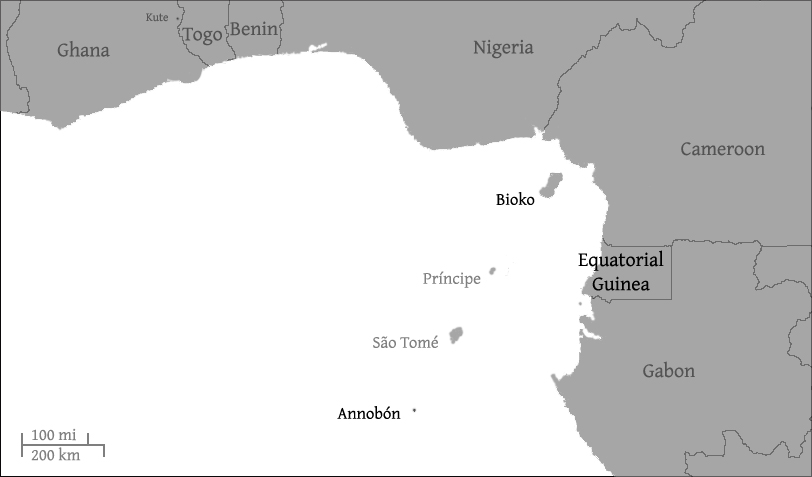
\includegraphics[width=.95\textwidth]{figures/yakpomod-img1.png}
	\label{map:1:1.1}
\end{figure}

\begin{figure}
	\caption*{Map 2 Towns with Pichi-speaking communities in Bioko (in bold)}
	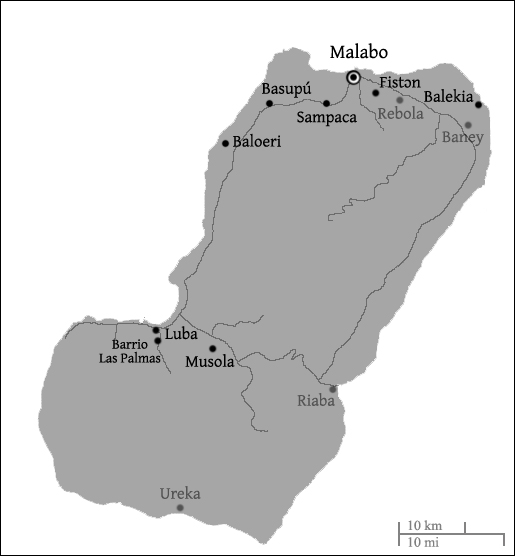
\includegraphics[width=.5\textwidth]{figures/yakpomod-img2.png}
	\label{map:1:1.2}
\end{figure}

The lingering colonialist perspective on Pichi and its sister languages in West Africa and across the Atlantic stands in stark contrast to the fact that these languages epitomise the achievements of African and African-descended peoples who, in resisting and adapting to the ignominious system of European slavery and colonialism, carved out in Africa and the Americas one of the largest, and today most vibrant cultural and linguistic zones of the world.

\section{Contact with Spanish}\label{sec:1.2}

\ili{Spanish} has left a deep imprint on the lexicon and grammar of Pichi. Codemixing is an integral part of the linguistic system of Pichi (\citealt{Yakpo2009complexity}, \citealt{Yakpo2018}). The pervasive influence of \ili{Spanish} on Pichi is for one part the consequence of language policy. Since colonial rule and the independence of Equatorial Guinea in 1968, Spanish has remained the sole medium of instruction at all levels of the educational system (\citealt[35–36]{Lipski1992}). There is a widespread competence in different registers of \ili{Spanish} by Pichi speakers in Malabo and Equatorial Guinea as a whole \citep{Lipski1985,García2016}. In Malabo, the acquisition of Spanish begins in early childhood, even for many working-class Equatoguineans with little or no school education. 

Another factor favouring codemixing is the positive attitude towards multilingualism in a highly polyglot society, against the background of a tenacious vitality of Pichi as a symbol of social identity. Presumably, Pichi-Spanish codemixing has for a long time served as a badge of identity for the population of Bioko in the course of a long history of immigration by speakers of other varieties of West African English-lexicon Creoles. Today, the language also plays an important role for the self-identification of those who grew up on the island in the face of an accelerated pace of internal migration by Equatoguineans from the mainland. \textit{Bɔ́n} \textit{na} \textit{yá,} \textit{gró} \textit{na} \textit{yá} ‘born here, grown up here’ is the mark which distinguishes Pichi-speaking islanders, irrespective of their ethnic background, from the late arrivals of mainland origin who speak little or no Pichi. 

Equally, the burgeoning oil economy of Equatorial Guinea has led to increased urbanisation, extending multi-ethnic social networks and the spread of Pichi as a native language. In such a socio-economic environment and amidst a high general competence in the official language Spanish, codemixing between Pichi and Spanish, rather than being exceptional, is consciously and confidently articulated in daily life (cf. chapter 11 for a detailed description of codemixing). Pichi is also in contact with other African languages spoken in the region, amongst them \ili{Fang} and \ili{Bube}, as well as \ili{Nigerian} and Cameroonian Pidgin (\citealt{Yakpo2013} discusses influences on Pichi from these languages).

\section{Variation}\label{sec:1.3}

The variation recorded in Pichi appears to be determined by a mixture of the factors age, language background, and social class. Phonological variation is particularly conspicuous. Some of the variation in Pichi may be captured by an albeit oversimplified division of speakers into two groups. Group 1 principally consists of the Fernandinos, the old commercial and social elite of Bioko \citep{Lynn1984} that inhabits the historical centre of Malabo and has used Pichi as a home language since the 19\textsuperscript{th} century. Group 1 also comprises people of diverse ethno-linguistic backgrounds who grew up in Malabo in the ambit of Fernandino culture. The lexicon, grammar, and phonology of Group 1 reflects an earlier chronolect of Pichi, which is also closer to (early) Krio. 

Group 2 is larger and culturally more diverse by incorporating “nuevos criollos” (Morgades Besari, p.c.) who have been accultured more recently into the Pichi-speaking urban culture of Malabo. It encompasses a large number of speakers with a \ili{Bube} cultural background who have shifted to Pichi as a primary language \citep{BolekiaBoleká2007}, and it includes large numbers of speakers with varying degrees of nativisation. Group 1 is shrinking at the expense of Group 2 through rapid urbanisation, immigration, and language shift. The terms “Mesopidgin” and “Acropidgin” employed by \citet{MorgadesBesari2011} capture some of the socio-linguistic differences between Group 1 and Group 2. The distinction between Group 1 and 2 is also reflected in apparent-time differences, where older speakers (principally those who came of age in the colonial era and the first decade of independence) tend to use the Group 1 lect, and the young majority population of Malabo and Bioko tends to use the Group 2 lect. 

In this work, I privilege the description of the language of Group 2 in the wish to represent how Pichi is spoken by the young and multi-ethnic majority in the homes and streets of Malabo today. I nevertheless account for variation by employing alternate forms where they exist (e.g. \textit{nɔ́bà{\textasciitilde}nɛ́a} ‘\textsc{neg.prf}’, \textit{tínap{\textasciitilde}tánap} ‘stand (up)’), and some of them may reflect differences between Groups 1 and 2. In the following, I present a few generalisations of the variation present in my corpus. 

For Group 2 speakers, there is no phonemic contrast between the alveolar fricative [s] and the postalveolar fricative [ʃ] (\hyperref[ex:0.1]{1}--\hyperref[ex:0.1.1]{2}), and this is systematically applied to all words where Group 1 speakers use [ʃ] (\hyperref[ex:0.2]{3}). Group 2 speakers also insert a palatal glide [j] between [s] and a following mid vowel where Group 1 uses [ʃ] alone (\hyperref[ex:0.3]{4}--\hyperref[ex:0.4]{5}):



% beginning of manual numbering of examples till (11)

% inserted ex:0.1.1 so manual numbering doesn't match with label numbering

\bigskip
\noindent\begin{tabularx}{\textwidth}{l ll lX}
% \lsptoprule
 &  & Group 1 &  Group 2 & \\
% \midrule
(1) \label{ex:0.1}
         & \itshape só & [só] & [só]  & ‘sew, like that’\\
(2) \label{ex:0.1.1}
         & \itshape só & [ʃó] & [só]  & ‘show’\\
(3) \label{ex:0.2}
         & \itshape fínis & [fínìʃ] & [fínìs] & ‘finish’\\
(4) \label{ex:0.3}
         & \itshape sɔ́p & [ʃɔ́p] & [sjɔ́p] & ‘shop’\\
(5) \label{ex:0.4}
         & \itshape nésɔn & [néʃɔ̀n] & [nésjɔ̀n] & ‘nation’\\
% \lspbottomrule
\end{tabularx}

\bigskip
Group 2 speakers tend to neutralise the phonemic distinction between close-mid and open-mid vowels (\hyperref[ex:0.5]{6}–\hyperref[ex:0.6]{7}):

\bigskip
\noindent\begin{tabularx}{\textwidth}{l ll lX}
 &  & Group 1 & Group 2 & \\
% \lsptoprule
(6) \label{ex:0.5}
         & \itshape fɔ & [fɔ̀] & [fò {\textasciitilde} fɔ̀] & ‘\textsc{prep}’\\
& \itshape mɔ́ & [mɔ́] & [mó {\textasciitilde} mɔ́] & ‘more’\\
(7) \label{ex:0.6}
         & \itshape mék & [mék] & [mék {\textasciitilde} mɛ́k] & ‘make, \textsc{sbjv}’\\
& \itshape lɛk & [lɛ̀k] & [lèk {\textasciitilde} lɛ̀k] & ‘like (preposition)’\\
% \lspbottomrule
\end{tabularx}

\bigskip
Group 2 speakers also tend to nasalise [i]-final words with an H.L tonal configuration (\hyperref[ex:0.7]{8}) and to prenasalise [j]-initial words as in (\hyperref[ex:0.8]{9}). This may lead to the formation of homophones like (\hyperref[ex:0.9]{10}) and (\hyperref[ex:0.10]{11}) for Group 2 speakers:

\bigskip
\noindent\begin{tabularx}{\textwidth}{l ll lX}
 &  & Group 1 & Group 2 & \\
% \lsptoprule
(8) \label{ex:0.7}
         & \itshape lɔ́ki & [lɔ́kì] & [lɔ́kìn] & ‘be lucky’\\
& \itshape tɔ́sti & [tɔ́stì] & [tɔ́stìn] & ‘be thirsty’\\
(9) \label{ex:0.8}
         & \itshape yandá & [jàndá] & [njàndá] & ‘yonder’\\
(10) \label{ex:0.9}
         & \itshape yús & [jús] & [njús] & ‘use’\\
(11) \label{ex:0.10}
         & \itshape nyús & [njús] & [njús] & ‘news’\\
% \lspbottomrule
\end{tabularx}



% end of manual numbering of examples
\addtocounter{equation}{11}

\bigskip
There is also some variation in the use and acceptance of certain grammatical structures. For example, Group 2 speakers seem to prefer the negative perfect marker \textit{nɛ́a} over \textit{nɔ́ba}. Equally, a serial verb construction\is{serial verb constructions} (SVC) featuring the verb \textit{sté} ‘be long time’ is not readily accepted as grammatical by many Group 1 speakers (cf. \sectref{sec:11.2.5}) and may therefore be a more recent development. Conversely, other types of SVCs are more common with Group 1 than with Group 2. Amongst them are SVCs involving the verb \textit{ték} ‘take’ (cf. \sectref{sec:11.2.3}) and motion-direction SVCs involving the verbs \textit{gó} ‘go’ and \textit{kán} ‘come’ (cf. \sectref{sec:11.2.1}). \textit{Ték}-serialisation is very common in modern \ili{Krio} and all other African English-lexifier creoles. Group 2 speakers instead tend to employ a combination of a verb and a prepositional phrase in these contexts. A final area characterised by variation is the extent of Pichi-Spanish language contact. For example, the names of weekdays and numerals are almost exclusively expressed in Spanish by Group 2 speakers. Group 1 speakers have access to both English- and Spanish-derived lexicon. They may employ \textit{lunes} ‘Monday’ in a codemixed sentence, but are equally likely to use \textit{mɔ́nde} ‘Monday’. Further, English-derived numbers above five are rarely used by Group 2 speakers (cf. \sectref{sec:13.3.1}). In contrast, Group 1 speakers master a wider range of the Pichi numeral system. However, even with this group, Pichi numbers above ten are seldom heard.

\section{Affiliation}\label{sec:1.4}
\largerpage
Pichi belongs to the grouping of languages referred to in the literature by various appelations, among them “English-based Afro-American” \citep{Alleyne1980}, “Atlantic Anglophone Creoles” \citep{Hancock1986,Hancock1987} “Atlantic English-based Creoles” (e.g. \citealt{MuyskenSmith1990}), “Atlantic English Creoles” (e.g. \citealt{Baker1999}). In this work and others, I employ the term “Afro-Caribbean English-lexifier Creoles” (abbreviated AECs) \citep{Faraclas2004} as a label that includes information about the speaker population (\mbox{“Afro-”}, i.e. people of African ancestry) and the two world regions where the languages are mainly spoken (“Afro-Caribbean”, i.e. Africa and the Caribbean). The use of “lexifier” underscores the dynamic character of the \ili{English} input to the lexicon, which varies in size and nature between the different languages. 


All Afro-Caribbean English-lexifier Creoles are transmitted and learned in various ways within the family and serve as means of communication and identification to linguistic communities. I therefore dispense with the term “pidgin” with its socio-structural connations and use “creole” alone. When referring to the linguistic grouping, “Creole” is written with an initial capital letter. The generic term is written “creole” in lower case. 

With well over 100 million speakers, the Afro-Caribbean English-lexifier Creoles and Pidgin-Creoles (henceforth AECs) spoken in Africa and the Americas together constitute one of the largest lectal continua of the Western hemisphere in speaker numbers and geographical extent \citep[22–23]{Yakpo2016estatuto}. Besides Pichi, the African sub-grouping of the AECs contains \ili{Krio} (Sierra Leone), \ili{Aku} (Gambia), Ghanaian Pidgin English, Nigerian Pidgin, and Cameroonian Pidgin \citep{HuberGörlach1996,Huber1999,BakerHuber2001}. There are also historical connections and cross-influences with varieties of Liberian English \citep{Singler1997}. Even if many details are still unclear, the evidence that there is a degree of common ancestry between the African and Caribbean AECs is compelling (e.g. \citealt{Hancock1986,Hancock1987,Smith1987,Smith2015}). There are also indications of a historical relation of the AECs with African American English(es) \citep{Dillard1973,Rickford1999,Winford2017}.

Within the African AECs, Pichi is most directly related to the \ili{Krio} language of Sierra Leone. A comparison of the two languages yields systematic lexical and structural correspondences. But it also reveals some differences. To begin with, both languages share a large percentage of non-basic vocabulary\is{basic vocabulary}, as shown in (\ref{ex:1:7}a), with the same tonal configurations. However, the Yoruba (b), Mende (c), and Temne (d) component of the Pichi lexicon appears to be much smaller than that of Krio and is limited to a few words in the corpus (data from \citealt{FyleJones1980}):

\eabox{\label{ex:1:7}
\begin{tabularx}{\textwidth}{rllX}
   & Pichi & Krio & Gloss\\
a. & \itshape a & \itshape a & ‘I’\\
& \itshape pɔ́sin & \itshape pɔ́sin & ‘person’\\
& \itshape (s)tík & \itshape (s)tík & ‘tree’\\
& \itshape yáy & \itshape yáy & ‘eye’\\
& \itshape yés & \itshape yés & ‘ear’\\
& \itshape bɔbí & \itshape bɔbí & ‘breast’\\
& \itshape bɛlɛ́ & \itshape bɛlɛ́ & ‘belly, foetus’\\
& \itshape watá, wɔtá & \itshape watá, wɔtá & ‘water’\\
& \itshape dɔtí & \itshape dɔtí & ‘be dirty’\\
& \itshape fɔdɔ́n & \itshape fɔdɔ́m & ‘fall’\\
& \itshape chɔ́p & \itshape chɔ́p, ít & ‘eat’\\
& \itshape hós & \itshape hós & ‘house’\\
& \itshape tití & \itshape tití & ‘girl’\\
& \itshape mákit & \itshape mákit, mákɛt & ‘market’\\
& \itshape wɔwɔ́ & \itshape wɔwɔ́ & ‘be messed up, ugly’\\
& \itshape bɔkú & \itshape bɔkú & ‘be much’\\
& \itshape yangá & \itshape nyangá & ‘be ostentatious’\\
& \itshape dúya & \itshape dúya & ‘please’\\
b. & \itshape ógi & \itshape ógi & ‘corn porridge’\\
& \itshape kúsɛ́ & \itshape kúshɛ́ & ‘expression of empathy’\\
& \itshape {}--- & \itshape órewá & ‘goodbye greeting’\\
c. & \itshape nyɔ́ní & \itshape nyɔ́ní & ‘red ant’\\
& \itshape blɔkɔ́s & \itshape blɔkɔ́s & ‘scrotum, penis’\\
& \itshape kandá & \itshape kandá & ‘skin, bark’\\
d. & \itshape yabaś & \itshape yabás & ‘onion’\\
& \itshape {}--- & \itshape kunkubé & ‘kind of boat’\\
\end{tabularx}
}
The two languages also share a number of lexical items common to numerous African and American English-lexicon Creoles. These were first compiled by (\citealt{Smith1987,Smith2001,Smith2015}) and termed “Ingredient X, Y, and Z”. In \REF{ex:1:8}, I list all the relevant words contained in the Pichi corpus. They comprise “Ingredient X” words of African origin (a), “Ingredient Y” words of Portuguese origin (b), “Ingredient Z” words of English origin (c), as well as a few function words of diverse origin (d):

\eabox{\label{ex:1:8}
\begin{tabularx}{.9\textwidth}{rll}
         & Ingredient X, Y, Z & Gloss\\
a. & \itshape sósó & ‘only’\\
& \itshape pɔtɔpɔ́tɔ́ & ‘mud(dy) substance’\\
& \itshape akará & ‘bean cake’\\
& \itshape fufú & ‘fufu’\\
b. & \itshape sabí & ‘know’\\
& \itshape pikín & ‘child’\\
c. & \itshape kéch & ‘catch’\\
& \itshape yɛ́r(i) & ‘hear’\\
& \itshape ɛf(ɛ) & ‘if’\\
& \itshape bwɛ́l & ‘boil’\\
& \itshape (s)pwɛ́l & ‘spoil, spend’\\
d. & \itshape na & ‘\textsc{foc}’\\
& \itshape una, unu & ‘\textsc{2pl}’\\
& \itshape mék & ‘imperative\is{imperatives}, \textsc{sbjv}’\\
& \itshape de & ‘\textsc{ipfv}’\\
& \itshape dé & ‘there’\\
& \itshape dé & \textsc{‘be.loc’}\\
\end{tabularx}
}
Some of the differences in vocabulary between the two languages owe to the same phonological characteristics that differentiate the members of Group 1 (Pichi) and Group 2 (\ili{Krio}) in the preceding section. Hence, most speakers of Pichi make no phonemic distinction between alveolar and postalveolar fricatives (\ref{ex:1:9}a); the phonemic distinction between close-mid and open-mid vowels is neutralised by most speakers (b). 

In addition, the distinction between velar and labial nasal consonants tends to collapse in word-final position (c); phonological processes create preferred CV sequences (d), voiced obstruents are normally devoiced in word-final position (e), while other words have different coda consonants (f). In general terms, present-day Pichi as spoken by the majority of its speakers exhibits a tendency towards the reduction of phonemic contrasts when compared to Krio.

\eabox{\label{ex:1:9}
\begin{tabularx}{\textwidth}{r ll ll ll}
 & \multicolumn{2}{l}{Pichi} & \multicolumn{2}{l}{Krio} & Gloss\\
a. & \itshape sút & [sút] & \itshape shút & [ʃút] & ‘shoot’\\
b. & \itshape fɔ & [fɔ̀{\textasciitilde}fò] & \itshape fɔ & [fɔ̀] & ‘\textsc{prep}’\\
c. & \itshape frɔn & [frɔ̀n {\textasciitilde} frɔ̀m] & \itshape frɔm & [frɔ̀m] & ‘from’\\
d. & \itshape smɔ́l & [sìmɔ́ {\textasciitilde} sùmɔ́] & \itshape smɔ́l & [smɔ́l] & ‘be small’\\
e. & \itshape bíg & [bík] & \itshape bíg & [bíg] & ‘be big’\\
f. & \itshape (s)trɔ́n & [(s)trɔ́n] & \itshape (s)trɔ́ng & [(s)trɔ́ŋ] & ‘be strong’\\
\end{tabularx}
}
Other differences in vocabulary, phonology, and grammar stem from the divergent socio-political development that Equatorial Guinea and Sierra Leone have gone through in the last hundred years. In Sierra Leone, British colonisation and the retention of political, economic, and linguistic ties with Britain after independence have reinforced the relationship between \ili{Krio} and \ili{English}. In Equatorial Guinea, the direct link with \ili{English} was severed in 1858 when Spanish assumed the role of the dominant language. Equally, the influence of \ili{Krio} on Pichi had petered out by the first decades of the 20\textsuperscript{th} century as Spanish colonialism gradually put a stranglehold on relations between Fernando Po and Sierra Leone. 

The role of the respective superstrates \ili{English} (for \ili{Krio}) and \ili{Spanish} (for Pichi) can be read from the impact of these two languages on institutional and administrative terminology (\ref{ex:1:10}a), the numeral system above ten (b), and other lexical items (c). The use of a larger number of English-derived lexical items in \ili{Krio} corresponds with a stronger presence of Spanish-derived lexicon in Pichi:

\eabox{\label{ex:1:10}
\begin{tabularx}{\textwidth}{rlll}
         & Pichi & Krio & Gloss\\
a. & \itshape profe(sor), tícha & \itshape tícha & ‘teacher’\\
& \itshape Camerún & \itshape Cameroon & ‘Cameroon’\\
& \itshape aeropuerto & \itshape ɛ́pɔt & ‘airport’\\
b. & \itshape diez & \itshape tɛ́n & ‘ten’\\
& \itshape doce & \itshape twɛ́lf & ‘twelve’\\
& \itshape las dos & \itshape tú oklɔ́k & ‘two o’clock’\\
c. & \itshape bikɔs, porque & \itshape bikɔs & ‘because’\\
& \itshape sube, gó ɔ́p & \itshape gó ɔ́p & ‘go up’\\
& \itshape sigue & \itshape kɔntínyu & ‘continue’\\
\end{tabularx}
}
There is a high degree of correspondence between the forms of Pichi and \ili{Krio} function words and the categories they express. For example, the forms and functions of the TMA\is{tense}\is{modality}\is{aspect} markers in \REF{ex:1:11} are largely coterminous: 

\eabox{\label{ex:1:11}
\begin{tabularx}{\textwidth}{llll}
Pichi & \ili{Krio} & Gloss\\
\itshape de & \itshape de & ‘\textsc{ipfv’}\\
\itshape go & \itshape go & ‘\textsc{pot}’\\
\itshape bin & \itshape bin & ‘\textsc{pst}’\\
\itshape dɔ́n & \itshape dɔ́n & ‘\textsc{prf}’\\
\itshape fɔ & \itshape fɔ & ‘\textsc{prep}’\\
\itshape kin & \itshape kin & ‘\textsc{hab}, \textsc{abl’}\\
\end{tabularx}
}
However, the distribution of the markers in \REF{ex:1:11} is not always identical in the two languages. For example, the \ili{Krio} data reveals more combinatorial possibilities of the habitual\is{habitual aspect} marker \textit{kin} ‘\textsc{hab}’ with other TMA markers (cf. \citealt{Dandeson2001}), while the Pichi imperfective marker \is{imperfective aspect} \textit{de} ‘\textsc{ipfv}’ seems to have a broader range of functions than the \ili{Krio} cognate form. Moreover, \ili{Krio} has at least two auxiliary constructions which are not attested in my data. The verb \textit{blánt} is only employed as a lexical verb with the meaning ‘reside’ in Pichi. In \ili{Krio}, the element \textit{blant} is a preverbal TMA element that expresses habitual aspect. Further evidence for grammaticalisation is that \textit{blant} is L-toned in this function. Consider the following example (Krio sentences are marked \textsc{Krio}):

\newpage 
\ea%12
    \label{ex:1:12}
\textsc{Krio}\il{Krio}\\
    \gll   Olú    \textbf{blant}  \textbf{gó}  London  fɔ  Krísmɛs.\\
\textsc{name}  \textsc{hab}    go  \textsc{place}  \textsc{prep}  Christmas\\

\glt ‘Olu always goes to London for Christmas.’  \citep[181]{YillahCorcoran2007}
\z

Further, \ili{Krio} employs the locative-existential copula \textit{dé} \textsc{‘be.loc’} together with the preposition \textit{pan} ‘on’ in an, albeit lectally restricted, auxiliary construction to express \isi{progressive aspect} \REF{ex:1:13}. The construction is rejected by Pichi speakers \REF{ex:1:14}:


\ea%13
    \label{ex:1:13}
\textsc{Krio}\il{Krio}\\
    \gll   \textit{Olú}   \textbf{dé}   \textbf{pan}    kám.\\
\textsc{name}  \textsc{be.loc}  on    come\\

\glt ‘Olu is coming (right now).’ \citep[179]{YillahCorcoran2007}
\z


\ea[*]{%14
    \label{ex:1:14}
    \gll   A    \textbf{dé}    \textbf{pan}   chɔ́p.\\
 \textsc{1sg.sbj}  \textsc{be.loc}  on    eat\\
\glt Intended: ‘I’m eating.’ [ye07je 025]
}\z

Conversely, there is no data to suggest the existence in \ili{Krio} of the Pichi egressive aspect construction involving the auxiliary verb \textit{kɔmɔ́t} ‘go/come out’ \REF{ex:1:15} or, obviously, the continuative aspect construction featuring the Spanish-derived verb \textit{sigue} ‘continue’ \REF{ex:1:16}. Equally, an adverbial SVC involving the V1 \textit{sté} ‘stay, be a long time’ appears to be unique to Pichi \REF{ex:1:17}: 


\ea%15
    \label{ex:1:15}
    \gll   Wì  \textbf{kɔmɔ́t}    \textbf{chɔ́p}  náw    só.\\
 \textsc{1pl}  come.out  eat    now    like that.\\
\glt ‘We just ate right now.’ [ge07fn 208]
\z


\ea%16
    \label{ex:1:16}
    \gll   A    \textbf{sigue}    \textbf{plé}    bɔ́l  sóté    ívin    tɛ́n.\\
\textsc{1sg.sbj}  continue    play    ball  until  evening  time\\

\glt ‘I continued playing ball until the evening.’ [be07fn 189]
\z


\ea%17
    \label{ex:1:17}
    \gll   A    \textbf{sté}  \textbf{chɔ́p}.\\
\textsc{1sg.sbj}  stay    eat\\

\glt ‘It’s been a long time since I ate.’ [au07ec 078]
\z

The literature on \ili{Krio} also indicates a wider range and a more pervasive use of SVCs than attested for Pichi. For instance, \ili{Krio} has a resultative SVC \is{resultative SVC}featuring dynamic verbs in the V2 position \REF{ex:1:18} and a \textsc{give}{}-type SVC in order to mark a recpient or beneficiary \REF{ex:1:19}. Both types of construction are not attested in Pichi:


\ea%18
    \label{ex:1:18}
\textsc{Krio}\il{Krio}\\
    \gll   Di  húman  \textbf{kúk}    rɛ́s    \textbf{sɛ́l}.                  \\
    \textsc{def}  woman  cook  rice    sell\\
\glt ‘The woman cooked rice and sold it.’ \citep[72]{Finney2004}
\z

\ea%19
    \label{ex:1:19}
\textsc{Krio}\il{Krio}\\
    \gll   I    \textbf{báy}    klós    \textbf{gí}    in    pikín.\\
\textsc{3sg.sbj}  buy    clothing  give    \textsc{3sg.poss}  child\\

\glt ‘He bought some clothes for his child.’ \citep[72]{Finney2004}
\z

In contrast, resultative state of affairs similar to \REF{ex:1:18} above may only feature stative property items as secondary verbs. Such constructions in Pichi are best seen to involve secondary predication \REF{ex:1:20}:


\ea%20
    \label{ex:1:20}
    \gll   Dɛn    dɔ́n    \textbf{bíl}   di  hós    \textbf{strɔ́n}.\\
\textsc{3pl}    \textsc{pfv}    build  \textsc{def}  road    be.strong\\

\glt ‘The house is solidly built.’ [ra07ve 069]
\z

At the same time, Pichi only employs a less integrated type of multiverb construction, namely clause chaining, in order to express a sentence like \REF{ex:1:19}, involving a dynamic V2. Note that unlike the \ili{Krio} sentences above, the Pichi example in \REF{ex:1:21} exhibits resumptive\is{resumptive pronouns} subject marking, i.e. the subject is repeated with the second verb in the series: 


\ea%21
    \label{ex:1:21}
    \gll   \textbf{Yu}  \textbf{ték}    di  mɔní  \textbf{yu}  \textbf{gí}  mí.\\
\textsc{2sg}  take    \textsc{def}  money  \textsc{2sg}  give  \textsc{1sg.indp}\\

\glt ‘You took the money (and) gave it to me.’ [ro05de 033]
\z

Numerous questions, however, remain open with regard to the extent of differences between the two languages. A considerable obstacle to comparative research is the lack of fresh data on Krio since the 1980s.

\section{Previous research on Pichi}\label{sec:1.5}

\citealt{Yakpo2009a} (in English) and \citeyear{Yakpo2010} (in Spanish) are the first in-depth descriptions of the phonology and grammar of Pichi. \citet{Zarco1938} is a language guide with a vocabulary list and a short grammar section. Trinidad Morgades Besari, former Vice-Chancellor of the National University of Equatorial Guinea and a well-known philologist of the country, has written about the use of \ili{Spanish} and Pichi in Equatorial Guinea \citep{MorgadesBesari2005,MorgadesBesari2011}. Morgades Besari’s unpublished work encompasses wordlists, a collection of stories and proverbs and proposals for an orthography of Pichi (see \citealt{Yakpo2011} for a discussion of the orthography). CEIBA Ediciones (Barcelona) has published a series of works dealing with the precolonial and colonial history and the political economy of Fernando Po, as well as the pivotal role of the Fernandinos in the making of present-day Bioko (e.g. \citealt{MartindelMolino1993}; \citealt{Cantús2006}).

\section{Standardisation and orthography}\label{sec:1.6}

No commonly accepted standard orthography is in use for Pichi. The transcription used in this work follows the Krio orthography employed in the seminal Krio-English Dictionary \citep{FyleJones1980} and subsequent revisions \citep{Coomber1992}, which, in turn, relies on the IPA-based Africa Alphabet \citep{InternationalAfricanInstitute1930} and the African Reference Alphabet \citep{UNESCO1981}. In the Krio\slash Pichi orthography, the grapheme <ɛ> renders the open-mid front vowel [ɛ], and <ɔ> renders the open-mid back vowel [ɔ]. Other vowel graphemes approximately also represent the corresponding IPA sounds. Pichi consonant phonemes and graphemes are presented in \tabref{tab:key:2.1}. In codemixed sentences, Spanish material is rendered using the standard Spanish orthography. 


Tone is marked on all Pichi words throughout this book. H-toned syllables bear an acute accent, e.g. \textit{wét} [wét] ‘wait’, and L-toned syllables remain unmarked, e.g. \textit{wet} [wèt] ‘with’. Tonal notation applies to the morpheme (i.e. the root), not the phonological word. In multimorphemic words, each morpheme therefore receives separate tone marks, e.g. \textit{ús=tɛ́n} \{\textit{\'us} ‘\textsc{q}’, \textit{tɛ́n} ‘time’\} ‘when’, \textit{fáyn-wán} \{\textit{fáyn} ‘nice’, \textit{-wán} ‘\textsc{adv}’\} ‘nicely’. Acute accents over Spanish words are orthographic, and hence not tone marks.


\section{Methods and data}\label{sec:1.7}

This grammatical description of Pichi is based on the analysis of a corpus of 46,060 words of dialogues, narratives, procedural texts, and elicitations. The data was collected during three stays of four weeks each in Malabo between 2003 and 2007 as part of the research for my PhD thesis \citep{Yakpo2009a}. Recordings were conducted in the quarters of Ela Nguema, Nyumbili, and the historical centre of Malabo. Recordings were done with a digital mini disc recorder and transcribed and analysed using the SIL Toolbox 1.5 programme. The analysis of tone was done from connected speech and words spoken in isolation using the Praat 5.0 software \citep{boersma2008}. Much of my approach is guided by linguistic typology and the descriptive apparatus developed in research on African languages. I try to describe as much variation as feasible. I largely avoid comparative or etymological observations with respect to English and African languages and try to look at Pichi “from the inside”. This grammar has also been published in Spanish \citep{Yakpo2010} in an abridged version for use in Equatorial Guinea by researchers and university students, teachers, and educationists. 


In Equatorial Guinea, I worked with altogether seventeen language consultants. All speakers have been using Pichi continuously since childhood onwards. Without exception, they are inhabitants of Malabo since birth or infancy. Most of them use Pichi more often than any other language, and most speakers view Pichi as the language they know best. Additionally, all speakers also know at least one of the following other languages in varying degrees of proficiency: \ili{Fang}, \ili{Bube}, \ili{Fa d’Ambô}, \ili{Kombe}, \ili{Lungwa Santome}, Nigerian Pidgin, \ili{Twi}, \ili{Spanish}, \ili{French}, \ili{English}, and \ili{German}. There is a bias in the data towards speakers with a Bube ethno-linguistic background, reflective of the circumstance that the majority of people who use Pichi as their primary language are from a Bube background. The numerical dominance by these “nuevos criollos” over the “old” Creole community of Fernandino descent (Morgades Besari, p.c.) represents a significant shift in the social dynamics of the language which is reflected in my choice of speakers. 



A few words are in order on aspects of my linguistic background and communicative approach during the research leading to this book. During my first stay in Malabo, I used Ghanaian Pidgin English and Spanish as working languages. During subsequent visits, when I felt confident enough to use Pichi without impeding fluid communication, I conducted my research exclusively in Pichi. My acquisition of Pichi and integration into social networks in Malabo was greatly facilitated by fluency in Ghanaian Pidgin English, competence in, and exposure to other Afro-Caribbean English-lexifier Creoles and West African languages, and a cultural and communicative \textit{savoir} \textit{faire} acquired during a childhood spent in Ghana. Fluency in French and Portuguese were also important resources in navigating the plurilingual landscape of Malabo and Bioko at various junctures during my research.


\tabref{tab:1:1.1} lists relevant information on language consultants. Speakers are sorted alphabetically along the “code” column. The symbol “N.N.” in the last row of the “speaker” column stands for incidental data collected from strangers in the streets, markets, and other public places in Malabo. Not included in the list is my own speaker code (ko). My participation in recorded conversations was kept to a minimum, but due to the nature of the method, it was more extensive during elicitations. Utterances of mine are, however, nowhere included in the analyses and interpretation of data. The symbols for gender are (F)emale and (M)ale. Age is provided in brackets of 10+, 20+, 30+, etc. The column “languages” specifies self-identified language knowledge. The symbol~(h) in the “languages” column indicates home languages used for interaction within the (extended) family. Languages are listed in alphabetical order but home languages come first. Basic information on social class can be deduced from the “activity” column. The column “residence” indicates the neighbourhood of Malabo in which the respective speakers are domiciled. Detailed information on the corpus is provided in \tabref{tab:1:1.2} further below.

%%please move \begin{table} just above \begin{tabular
%\begin{table}

\begin{longtable}{>{\footnotesize}l@{~}>{\footnotesize}l@{~} >{\footnotesize}l@{~}>{\footnotesize}l >{\footnotesize\raggedright}p{3cm} >{\footnotesize\raggedright}p{2cm} >{\footnotesize}l}
\caption{Language consultants}\label{tab:1:1.1}
\\
\lsptoprule

Code & Speaker & F/M & Age & Languages & Activity & Residence\\
\midrule\endhead
ab & Abuela & \textsc{F} & 80+ & Bube~(h), Pichi~(h), 

Spanish~(h) & Child rearing, farming & Town\\
au & Agustín & M & 30+ & Fang~(h), Spanish~(h), Pichi, French & Senior civil service & Ela Nguema\\
be & Beatriz & \textsc{F} & 20+ & Bube~(h), Pichi~(h), Spanish & Child rearing & Ela Nguema\\
bo & Aboki & \textsc{F} & 40+ & Pichi~(h), Spanish~(h), Bube & Trade & Town\\
ch & Charlie & M & 10+ & Pichi~(h), Spanish & School goer & Ela Nguema\\
dj & Djunais & M & 20+ & Pichi~(h), Spanish~(h), Bube & Cook & Ela Nguema\\
eb & Ebongolo & M & 20+ & Kombe ~(h), Pichi, Spanish &  & Ela Nguema\\
ed & Eduardo & M & 30+ & Fa d’Ambô~(h), Lungwa Santome~(h), Fang, English, Pichi, Spanish & Civil servant & Ela Nguema\\
f1 & Fita 1 & M & 20+ & Unknown & Mechanic & Nyumbili\\
f2 & Fita 2 & M & 20+ & Unknown & Mechanic & Nyumbili\\
fr & Francisca & \textsc{F} & 30+ & Pichi~(h), Spanish~(h), English, French & Civil servant & Ela Nguema\\
ge & Lage & \textsc{F} & 30+ & Pichi~(h), Spanish~(h), English & Restaurant owner & Ela Nguema\\
he & Hermina & \textsc{F} & 30+ & Kombe ~(h), Fang, Pichi, Spanish & Child rearing & Ela Nguema\\
hi & Hilda & \textsc{F} & 50+ & Pichi~(h), Spanish~(h), Bube, English & Trade & Town\\
ku & Tía Kuki & \textsc{F} & 50+ & Kombe ~(h), Fang, Pichi, Spanish & Trade & Ela Nguema\\
kw & Kwame & M & 40+ & Twi~(h), English, Pichi, Spanish & Security guard & Kolwatá\\
li & Lindo & M & 30+ & Kombe ~(h), Pichi~(h), Spanish & Worker & Ela Nguema\\
lo & Lourdes & \textsc{F} & 30+ & Pichi~(h), Spanish~(h), English & Manager & Town\\
ma & María & \textsc{F} & 30+ & Bube~(h), Pichi~(h), Spanish & Domestic worker & Nyumbili\\
mi & Miguel & M & 10+ & Pichi~(h), Spanish~(h), Bube & School goer & Town\\
ne & Nenuko & M & 30+ & Pichi~(h), Spanish~(h), Bube & Mechanic & Ela Nguema\\
pa & Pancho & M & 20+ & Pichi~(h), Spanish~(h), Bube & Hustler & Ela Nguema\\
ra & Maura & \textsc{F} & 20+ & Pichi~(h), Spanish~(h), Bube & Secretary & Los Angeles\\
ro & Mami Rose & \textsc{F} & 50+ & Bube~(h), Pichi~(h), Spanish & Domestic worker & Ela Nguema\\
sa & Don Samuel & M & 70+ & Kombe ~(h), Fang, Pichi, Spanish & Entre-preneur & Town\\
to & Tía Tokó & \textsc{F} & 50+ & Bube~(h), Pichi~(h), Spanish~(h), Nigerian Pidgin, English & Accountant & Town\\
tr & Doña Trinidad & \textsc{F} & 70+ & Pichi~(h), Spanish~(h), English, French & Academic & Town\\
ur & Ursus & M & 30+ & Pichi~(h), Bube, Spanish & Worker & Ela Nguema\\
ye & Boyé & M & 20+ & Pichi~(h), Spanish~(h), Bube & Worker & Ela Nguema\\
nn & N.N & M/\textsc{F} & Div. & Diverse & Diverse & Diverse\\
\lspbottomrule
\end{longtable}
%\end{table}

\tabref{tab:1:1.2} provides information on the corpus. The list is sorted alphabetically according to the “text code” column, which lists the name of the text (e.g. 03ab). Text names were given according to mnemonic principles. An “e” at the end of text code indicates that the text consists of elicited data (e.g. 05ae). The “type” column indicates the text genre, “contents” provides a short description of the text. The column entitled “word count” provides an indication of the relative length of texts. An asterisk (*) after the “text code” indicates that the corresponding text is contained (in part or in full length) in the text section of this book.

%%please move \begin{table} just above \begin{tabular
%\begin{table}

\begin{longtable}{l >{\raggedright}p{2.1cm} >{\raggedright}p{4.5cm} lr}
\caption{Corpus}\label{tab:1:1.2}\\
\lsptoprule

Text & Type & Contents & Speakers & Word\\
code & & & & count\\
\midrule
\endhead
03ab* & Narrative & Sickness & ab, fr & 1911\\
03ay & Narrative & Youth memories & ab & 2384\\
03cb & Conversation & Female-male relations & hi, bo & 2872\\
03cd* & Conversation & House-building; joking; home affairs & dj, fr, ko, ye & 1827\\
03do* & Procedure & Preparation of a dish & dj & 778\\
03ft & Narrative & Family history & fr & 2771\\
03wt* & Narrative; conversation & Supernatural encounter & dj, fr, ru & 813\\
03fp & Procedure & Car maintenance & f1, f2, kw & 274\\
03gm & Narrative & Language issues & to & 683\\
03hm & Narrative & Working in Gabon & ma & 3983\\
03ni & Conversation & Life in Nyumbili & ma, ko & 468\\
03sb & Narrative; procedure & Supernatural encounters & ed, kw & 3073\\
03sh & Narrative & Anecdotal story & ma & 291\\
03sp & Narrative & Student days in Cuba & ed, kw & 1324\\
05ae & Elicitation & Complementation; lexical aspect & dj, ye & 1930\\
05be & Elicitation & Spatial relations & dj & 1431\\
05ce & Elicitation; conversation & Basic vocabulary; metalinguistic discussion & dj, pa, ye & 2329\\
05de & Elicitation & Relativisation; adverbial relations; questions & ro & 620\\
05ee & Elicitation & Copula meanings & ro & 1101\\
05fe & Elicitation & Colours, numbers, time & ro & 256\\
05rr & Conversation; procedure & Cooking at home & ro, ye & 1278\\
05rt & Narrative & Marital affairs & ro, ye & 891\\
07ae & Elicitation & Grammatical relations & dj & 3213\\
07ce & Elicitation & Derivation & au & 739\\
07de & Elicitation & Double objects & ye & 205\\
07he & Elicitation & Questions; conversation & be, lo & 242\\
07je & Elicitation & Pragmatic routines & ye & 1072\\
07fn & Conversation & Field notes & Diverse & 1304\\
07ga* & Conversation & Anecdotal story; joking & la, ne, ye & 430\\
07me & Elicitation & Multiverb constructions & pa & 1077\\
07pe* & Elicitation (video) & Caused positions & li, dj & 783\\
07re & Elicitation (video) & Reciprocity & dj & 494\\
07se & Elicitation (video); conversation & Staged events; metalinguistic discussion & au, fr, ra & 2649\\
07ve & Elicitation & Derivation & ra & 571\\
\lspbottomrule
\end{longtable}
%\end{table}
The corpus presented in \tabref{tab:1:1.2} consists of altogether thirty-four texts of different genres totalling 46,060 words. Based on the figures of the “word count” column, narratives constitute approximately 37 per cent of the total corpus (the word count of texts with two genres has been divided by two). This genre encompasses life stories and family histories, illness and near-death accounts, supernatural encounters and other emotionally charged experiences, as well as travel and life abroad. Conversations amount to 25 per cent of the corpus. The topics range from house-building to gender relations, from jesting and joking to metalinguistic discussions during elicitation. In many of the conversations recorded, in particular those involving peer-to-peer communication, form is just as important as content. These conversations “for their own sake” are characterised by emphatic, expressive, and figurative language. 

Procedural texts form some 7 per cent of the corpus. They describe various types of routines, for example the preparation of dishes, car maintenance and repair, medical treatment and sorcery, habits and ways of doing things. Elicitation makes up about 33 per cent of the corpus. I employed oral (Spanish to Pichi and monolingual Pichi-based) elicitation to obtain data chiefly on grammatical relations, the classification of situations (i.e. dynamic vs. non-dynamic verbs vs. adjectives), complementation, relativisation, and derivation. I made use of visual, video-based elicitation to uncover the expression of spatial relations including caused positions, the expression of certain complex events (“staged events”), and reciprocity. The video clips of the Language and Cognition Group of the Max-Planck Institute for Psycholinguistics in Nijmegen provided the basis for these elicitiations. Most elicitations were conducted in groups of two or three speakers. This produced valuable data on variation and encouraged vivid metalinguistic discussions during the exercise. 

\section{Presentation of the data}\label{sec:1.8}
% \figref{fig:1:1.1} below shows how language data is presented in this work. Explanations are provided for the elements in the example:
% 
% \begin{figure}
% \caption{1 Presentation of data}
% \label{fig:1:1.1}
%  Relevant features in \textbf{bold}\\
% \begin{exe}
% \exi{\textsf{Example no.}} 
% \exi{(22)}
%  \gll A    kɛ́r=an      gó  na  comedor. \textsf{\upshape Pichi line}\\
% \textsc{1sg.sbj}  carry=\textsc{3sg.obj}    go  \textsc{loc}  dining-room \textsf{Interlinear gloss line}\\
% \glt ‘I carried him to the dining-room.’ \textsf{Free translation line}  [{ab}{03}{ab} {091}] \textsf{code}\\
% % \tikzmark{y1}{Speaker name} \hspace*{2cm} \tikzmark{y2}{year recorded}\hspace*{2cm}  \tikzmark{y3}{text name}\hspace*{2cm}  \tikzmark{y4}{sentence no. in text}
% \end{exe}
% % \connect{x1}{y1}
% % \connect{x2}{y2}
% % \connect{x3}{y3}
% % \connect{x4}{y4}
% \todo[inline]{braucht man vllt nicht. Erklärung der Codes wäre ausreichend IMHO}
% \end{figure}

In examples, the free translation is followed by a text code in squared brackets. Whenever an example features elicited data, the second letter of the text code is an “e”, e.g. [dj07ae 137] and [ra07ve 069]. Common parentheses in the free translation line contain supplementary and disambiguating translation material. Squared brackets provide contextual or other relevant meta-information. Punctuation in the Pichi examples follows intonation: A full stop indicates an utterance-final boundary tone, a comma continuative intonation. A slash denotes a speech interruption and hence an incomplete sentence. \ili{Spanish} words are rendered in the Spanish orthography. I do not provide category labels for Spanish grammatical morphemes where they occur, since this would have complicated interlinear glossing and given Spanish material undue prominence. 

A final note is in order on the notion of frequency employed throughout this work. When an exact percentage is not given, certain expressions may indicate the relative frequency or importance of a phenomenon. The expressions in the left column of \tabref{ex:1:23} correspond approximately to the percentages given in the right column \citep{MichaelisEtAl2013}.

\begin{table}
\caption{Frequency of phenomena}
\label{ex:1:23}
\begin{tabularx}{\textwidth}{lY}
\lsptoprule
Expression& Approximate percentage\\
\midrule 
Pervasive, the overwhelming majority, the vast majority & 90\%\\
The majority, very common, a high frequency & 70\%\\
About half, equally often, fairly common & 50\%\\
The minority, a low frequency & 30\%\\
Marginal, a small minority, a small number, seldom, rare & 10\%\\
\lspbottomrule
\end{tabularx}
\end{table}

 %redo map 
% \chapter{Segmental phonology}

The phonological system of Pichi features a phoneme inventory of twenty-two consonants and seven vowels. There is a good deal of free and allophonic variation in the use of these phonemes. Phonological processes include nasalisation, the use of clitics and the appearance of a linking /r/ during cliticisation, as well as the reduction of consonant clusters by deletion and insertion. In general, however, Pichi speakers tend to fully articulate consonants and vowels. The majority of Pichi words consist of one or two syllables. There are no phonemic long vowels but words may feature clusters of up to three consonants. The segmental system of Pichi interacts in various ways with the suprasegmental system (cf. chapter 3).

\section{Consonants}\label{sec:2.1}

The maximal inventory of twenty-two consonant phonemes in Pichi is presented in IPA symbols in \tabref{tab:key:2.1}. Details on the status and distribution of these phonemes are discussed in sections \sectref{sec:2.2} and \sectref{sec:2.6.2.1}.

%%please move \begin{table} just above \begin{tabular
\begin{table}
\caption{Consonant and approximant phonemes}
\label{tab:key:2.1}
\fittable{
\small
\begin{tabular}{lllllllllllllllll}
\lsptoprule

& 
 \multicolumn{2}{p{15mm}}{Bilabial} &
 \multicolumn{2}{p{15mm}}{Labio-dental} & 
 \multicolumn{2}{p{15mm}}{(Post-)\newline alveolar} & 
 \multicolumn{2}{c}{Palatal} & 
 \multicolumn{2}{c}{Velar} & 
 \multicolumn{2}{p{10mm}}{Labio-velar} & 
 \multicolumn{2}{c}{Uvular} & 
 \multicolumn{2}{c}{Glottal}\\
\midrule 
Stop & p & b &  &  & t & d &  &  & k & g & kp & gb &  &  &  & \\
Affricate &  &  &  &  & tʃ & dʒ &  &  &  &  &  &  &  &  &  & \\
Fricative &  &  & f & v & s &  &  &  &  &  &  &  &  & ʁ &  & h\\
Nasal &  & m &  &  &  & n &  & ɲ &  & ŋ &  &  &  &  &  & \\
Liquid &  &  &  &  &  & l &  &  &  &  &  &  &  &  &  & \\
Approximant &  &  &  &  &  &  &  & j &  & w &  &  &  &  &  & \\
\lspbottomrule
\end{tabular}
}
\end{table}
The (near-)mininal pairs in \tabref{tab:key:2.2} establish the phonemic status of the segments contained in \tabref{tab:key:2.1}.

%%please move \begin{table} just above \begin{tabular
\begin{table}
\caption{Consonant phoneme minimal pairs}
\label{tab:key:2.2}

\begin{tabularx}{\textwidth}{Qlll@{\qquad\qquad} lll}
\lsptoprule
/p/  /b/ & \itshape plánt & [plánt] & ‘plant’ & \itshape blánt & [blánt] & ‘reside’\\
/t/  /d/ & \itshape tɛ́n & [tɛ́n] & ‘time’ & \itshape dɛ́n & [dɛ́n] & ‘\textsc{3pl.indp}’\\
/k/  /g/ & \itshape kɔ́n & [kɔ́n] & ‘corn’ & \itshape gɔ́n & [gɔ́n] & ‘gun’\\
/tʃ/  /dʒ/ & \itshape chɔ́ch & [tʃɔ́tʃ] & ‘church’ & \itshape jɔ́ch & [dʒɔ́tʃ] & ‘(to) judge’\\
/f/  /p/ & \itshape fát & [fát] & ‘fat’ & \itshape pát & [pát] & ‘part’\\
/v/  /b/ & \itshape greví & [grèví] & ‘gravy’ & \itshape bebí & [bèbí] & ‘baby’\\
/s/  /t/ & \itshape sɔn & [sɔ̀n] & ‘some’ & \itshape tɔ́n & [tɔ́n] & ‘town’\\
/r/  /l/ & \itshape rɔ́n & [rɔ́n] & ‘run’ & \itshape lɔ́n & [lɔ́n] & ‘be long’\\
/h/  ø & \itshape hól & [hól] & ‘hole’ & \itshape ól & [ól] & ‘be old’\\
/m/  /n/ & \itshape motó & [motó] & ‘car’ & \itshape nóto & [nótò] & ‘\textsc{neg}.\textsc{foc}’\\
/ŋ/  /n/ & \itshape tɔ́n & [tɔ́n] & ‘town’ & \itshape tɔ́ng & [tɔ́ŋ] & ‘tongue’\\
/ɲ/  /y/ & \itshape nyú & [ɲú] & ‘be new’ & \itshape yú & [jú] & ‘\textsc{2sg.indp}’\\
/j/  /w/ & \itshape yés & [jés] & ‘ear’ & \itshape wés & [wés] & ‘buttocks’\\
/kp/ /gb/ & \itshape kpu & [kpù] & ‘\textsc{ideo}’ & \itshape gbin & [gbìn] & ‘\textsc{ideo}’\\
\lspbottomrule
\end{tabularx}
\end{table}
\section{Consonant allophony and alternation}\label{sec:2.2}

/\textbf{b}/ and /\textbf{v}/:

The voiced labio-dental plosive /v/ is a phoneme in its own right in a small number of words, where it does not alternate with /b/, e.g. \textit{greví} [grèví] ‘gravy’ and \textit{gív=an} [gívàn] ‘give him/her/it’. In a second group of words, /v/ is in free variation with /b/, e.g. \textit{vájin} [bádʒìn{\textasciitilde}vádʒìn] ‘virgin’, \textit{ívin} [íbìn{\textasciitilde}ívìn] ‘evening’, \textit{óva} [óbà{\textasciitilde}óvà] ‘over, be excessive’, \textit{sɛven} [sɛ́bèn{\textasciitilde}sɛ́vèn] ‘seven’, and \textit{ríva} [ríbà{\textasciitilde}rívà] ‘river’. Free variation is also encountered in the \ili{Spanish}-derived lexicon of most speakers, as in \textit{abuela} [abwɛla{\textasciitilde}aßwela{\textasciitilde}avwɛla] ‘grandmother’. 


In a third group of words, we only find /b/, which therefore does not alternate with /v/. Hence, we find \textit{fíba} [fíbà] ‘resemble’, \textit{líba} [líbà] ‘liver’, \textit{súb} [súb] ‘shove’, \textit{híb} [híb] ‘throw’, \textit{bába} [bábà] ‘cut hair’, and \textit{dɛ́bul} [dɛ́bùl] ‘devil’. The orthographic representation chosen for words of the second group, in which we find free alternation between [b] and [v], is <v>. Alternating words are given with both variants in the Pichi-English vocabulary section.


/\textbf{tʃ}/ and /\textbf{dʒ}/:

The voiceless postalveolar affricate tends to be unstable with many speakers and optionally alternates with the voiceless palatal plosive [c] and sometimes with the voiceless postalveolar fricative [ʃ], particularly in word-final position. Hence we find \textit{tɔ́ch} [tɔ́tʃ\textasciitilde tɔ́c\textasciitilde tɔ́ʃ] ‘touch’. A small number of speakers, all of which belong to Group 1 (cf. \sectref{sec:1.3}) exhibit allophonic variation between /tʃ/ and /dʒ/ in some words, with the latter allophone appearing in word-final position before the clitic \textit{=an} ‘\textsc{3sg.obj}’, i.e. \textit{jɔ́ch=an} [dʒɔ́dʒàn] ‘judge him/her/it’. 


The vast majority of speakers, however, and Group 1 speakers in particular, use word-final /tʃ/ in every environment including ones which are not prone to devoicing, i.e. \textit{chénch=an} [tʃéntʃàn] ‘change him/her/it’. I have accounted for the fact that most speakers exhibit no such variation by opting for <ch> in the orthography even though word-final /tʃ/ may be an allophone of /dʒ/ for a minority of speakers in words like \textit{jɔ́ch} ‘judge’ (but not in others, e.g. \textit{kéch} ‘catch’).


/\textbf{s}/:

The voiced alveolar fricative [z] is attested as a free variant of the voiceless alveolar fricative between two vowels in word-medial position, e.g. \textit{ísi} [ízì{\textasciitilde}ísì] ‘be easy’ and \textit{lési} [lézì{\textasciitilde}lésì] ‘be lazy’. I take [z] to be a non-phonemic variant of /s/ in these words. 


Furthermore, most Group 1 speakers (cf. \sectref{sec:1.3}) apply an opposition between /s/ and /ʃ/ (rendered by the grapheme <sh>), which produces minimal pairs like \textit{só} [só] ‘sew’ and \textit{shó} [ʃó] ‘show’. For Group 2 speakers, this opposition is, however, neutralised in favour of /s/, and they employ the voiceless alveolar fricative [s] in any position in which Group 1 speakers may use the voiceless postalveolar fricative [ʃ]. Group 2 speakers therefore produce homonyms like \textit{só} [só] ‘sew’ and \textit{só} [só] ‘show’.



Additionally, Group 2 speakers usually insert a palatal glide /j/ between /s/ and either of the mid vowels /e/ and /ɔ/ where Group 1 speakers only employ /ʃ/{\fff}. This inter-group variation applies to the following words in the data: \textit{kwɛ́sɔn} [kwɛ́sjɔ̀n{\textasciitilde}kwɛ́sʃɔ̀n] ‘question’, \textit{nésɔn} [nésjɔ̀n{\textasciitilde}néʃɔ̀n] ‘nation(ality)’, \textit{séb} [sjéb{\textasciitilde}ʃéb] ‘share’, \textit{sék} [sjék{\textasciitilde}ʃék] ‘shake’, \textit{sém} [sjém{\textasciitilde}ʃém] ‘shame’, \textit{sɔ́t} [sjɔ́t{\textasciitilde}ʃɔ́t] ‘be short, shirt’, \textit{sén} [sjén{\textasciitilde}sén] ‘same’, and \textit{sɔ́p} [ʃɔ́p] ‘shop’. Although the insertion of /j/ is optional, it is very common with the words listed. The insertion of /j/ is, however, not generalised to two other words in the corpus featuring a sequence of the phonemes /sé/. Hence, we find \textit{sé} [sé] ‘quot’ and \textit{fɔséka} [fɔ̀sékà] ‘due to’. 



The orthography does not represent the segment /j/ in words to which insertion applies. The words that exhibit this alternation are listed in the preceding paragraph and are additionally identified in the Pichi-English vocabulary. 


/\textbf{n}/ and /\textbf{m}/: 

The realisation of the alveolar nasal /n/ and the bilabial nasal /m/ is conditioned by a number of factors, which are covered in \sectref{sec:2.5.2}. 

/\textbf{nj}/ and /\textbf{ɲ}/:

A prothetic /n/ is optional (and present in at least half of the occurrences recorded) in a specific group of words with an underlying word-initial /j/. The relevant words are \textit{yandá} [jàndá{\textasciitilde}njàndá] ‘yonder’, \textit{yún} [jún{\textasciitilde}njún] ‘be young’ and \textit{yús} [jús{\textasciitilde}njús] ‘use’. In this group of words, I therefore analyse the combination of these segments as a cluster consisting of the alveolar nasal /n/ and the palatal approximant /j/.\is{insertion of segments}


In a second, equally small group of words, I posit the phoneme /ɲ/, compare the minimal pair \textit{nyú} [ɲú] ‘be new’ vs. \textit{yú} [jú] \textsc{‘2sg.indp’}. The other words that do not alternate in my data and therefore appear to feature a word-initial /ɲ/ rather than the cluster /nj/ are \textit{nyangá} [ɲàŋgá] ‘put on airs’, \textit{nyankwé} [ɲànkwé] ‘(the) nyankwé (dance)’, \textit{nyɔ́ní} [ɲɔ́ní] ‘ant’, and \textit{nyús} [ɲús] ‘news’. The phoneme /ɲ/ is also found in a word-medial, syllable onset position in two words in the corpus, namely in the place name \textit{Panyá} [pàɲá] ‘Spain’ and in the ideophone \textit{ményéményé} [méɲéméɲé] ‘whine, nag in a childlike fashion’.



A third group of words with a word-initial /j/ does not usually exhibit nasal prothesis at all, e.g. \textit{yɛ́s} [jɛ́s] ‘yes’, \textit{yét} [jét] ‘yet’, \textit{yɛ́stadé} [jɛ́stàdé] ‘yesterday’, and \textit{yáy} [jáj] ‘eye’. In the orthography, I only render an initial /n/ with the second group of words, i.e. words that feature the phoneme /ɲ/. Words with an optional prothetic /n/ are listed above and given with their alternate forms in the Pichi-English vocabulary.


/\textbf{j}/:

This voiced palatal approximant is a phoneme in its own right in words like \textit{yú} [jú] \textsc{‘2sg.indp’}, \textit{yá} [já] ‘here’, \textit{yɛ́s} [jɛ́s] ‘yes’ and \textit{yét} [jét] ‘yet’. Besides that, some words with a word-initial /j/ optionally appear with a prothetic /n/ (cf. on /n/ below). The segment /j/ is also optionally inserted between /s/ and one of the mid-vowels /e/ and /ɔ/ in another group of words (cf. on /ʃ/ below). {\fff}


Further, /j/ is optionally inserted between either of the velar consonants /g/ and /k/ and the front vowels /a/ and /ɛ/. However, this process only applies to a few relevant words of English origin with which it occurs in the majority of instances. The corpus contains the following words to which this applies: \textit{gádin} [gádìn{\textasciitilde}gjádìn], \textit{gál} [gál{\textasciitilde}gjál] ‘girl’, \textit{gɛ́l} [gɛ́l{\textasciitilde}gjɛ́l] ‘girl’, \textit{káp} [káp{\textasciitilde}kjáp] ‘cap’, \textit{kápinta} [kápìntà{\textasciitilde}kjápìntà] ‘carpenter’, and \textit{kɛ́r} [kɛ́r{\textasciitilde}kjɛ́r] ‘carry’. In contrast, a /j/ is not normally inserted in other words of English origin like \textit{gɛ́t} [gɛ́t] ‘get’, \textit{kán} [kán{\textasciitilde}kám] ‘come’, and \textit{káyn} [kájn] ‘kind’, as well as a group of words of non-English origin with an L.H pitch pattern, amongst them \textit{garí} [gàrí] ‘garí’, \textit{kaká} [kàká] ‘defecate’, \textit{kasára} [kàsárà] ‘cassava’, and \textit{kandá} [kàndá] ‘skin’. 



The orthography does not render the epenthetic /j/ in words that feature it. All relevant words are listed above and are identified in the Pichi-English vocabulary section. 


/\textbf{r}/:

The symbol /r/ varies in pronounciation between that of a voiced uvular fricative [ʁ] and a velar fricative [ɣ]. Some speakers use an alveolar tap [ɾ] instead of these two segments, and I have also occasionally heard an uvular trill [ʀ]. We therefore find variants like the following: \textit{máred} [máʁèd{\textasciitilde}máɣèd{\textasciitilde}máɾèd] ‘marry’, \textit{dríng} [dʁíng{\textasciitilde}dɣíng{\textasciitilde}dɾíng] ‘drink’, \textit{kɛ́r} [kɛ́ʁ{\textasciitilde}kɛ́ɣ{\textasciitilde}kɛ́ɾ] ‘carry’, and \textit{rɛ́s} [ʁɛ́s{\textasciitilde}ɣɛ́s{\textasciitilde}ɾɛ́s] ‘rice’. The orthography represents this segment as <r> and as [r] for phonemic and phonetic transcriptions.

/\textbf{h}/:

This voiced glottal fricative is phonemic in a small group of words which is delineated by minimal pairs like \textit{hól} [hól] ‘hole, hold’ vs. \textit{ól} [ól] ‘be old’. The group contains words like \textit{hát} [hát] ‘hurt, heart’, \textit{hála} [hálà] ‘shout’, \textit{hós} [hós] ‘house’, and \textit{héd} [héd] ‘head’. The group also includes two words with a word-medial /h/, namely \textit{bihɛ́n} [bìhɛ́n] ‘behind’ and \textit{wahála} [wàhálà] ‘trouble’. 


With a second and larger group, /h/ may be inserted at the beginning of the vowel-initial word. Such a prothetic /h/, although optional, occurs more often than not with most words in this group. Hence we find variants like \textit{ánsa} [ánsà\textasciitilde hánsà] ‘respond’, \textit{áks} [áks\textasciitilde háks] ‘ask’, \textit{ópin} [ópìn\textasciitilde hópìn] ‘open’, and \textit{évi} [évì\textasciitilde ébì\textasciitilde hévì\textasciitilde hébì] ‘be heavy’. In some instances, it is however impossible to determine whether a word-initial /h/ is prothetic or part of the segmental structure of a word, because the data contains no recorded instance without an initial /h/. Some of the words to which this applies are \textit{húman} ‘woman’, \textit{hɛ́lp} ‘help’, \textit{hébul} ‘be able’, \textit{hía} ‘year’, \textit{hásis} ‘ashes’, and \textit{hós} ‘house’. I have chosen to render these words with an initial <h>.{\fff}



A third group of vowel-initial words is not attested with a prothetic /h/, e.g. \textit{óva} [óvà] ‘be excessive, over’; \textit{ónli} [ónlì] ‘only’, \textit{áfta} [áftà] ‘then’, and \textit{éch} [étʃ] ‘age’. In the orthography, the segment /h/ is only represented with words that always appear with a word- or syllable-initial /h/. 


/\textbf{gb}/ and /\textbf{kp}/:

These two voiced and voiceless labiovelar plosives are marginally phonemic and only occur in a handful of ideophones\is{ideophones}, e.g.\textit{ nák gbin} ‘hit \textsc{ideo}’ = ‘hit hard and unexpectedly’, \textit{sút kpu} ‘shoot \textsc{ideo}’ = ‘shoot followed by the sound of a dull impact on the body’.

\section{Vowels}\label{sec:2.3}

The following seven vowel phonemes are found in Pichi. Vowel length is not distinctive. Consonant allophony and alternation are discussed below:

%%please move \begin{table} just above \begin{tabular
\begin{table}
\caption{Vowel phonemes}
\label{tab:key:2.3}

% \begin{tabularx}{\textwidth}{lXXXXXX}
%  & \multicolumn{3}{c}{Front} & \multicolumn{2}{c}{Central} & Back\\
% \lsptoprule
% Close & i &  &  &  &  & u\\
% Close-mid &  & \biberror{[F065?]} &  &  &  & o\\
% Open-mid &  &  & ɛ &  &  & ɔ\\
% Open &  &  &  & a &  & \\
% \lspbottomrule
% \end{tabularx}
\begin{tikzpicture}
 \aeiouEO
\end{tikzpicture}

\end{table}
The following (near-)minimal pairs establish the phonemic status of the segments contained in \tabref{tab:key:2.3}:

%%please move \begin{table} just above \begin{tabular
\begin{table}
\caption{Vowel phoneme minimal pairs}
\label{tab:key:2.4}

\begin{tabularx}{.66\textwidth}{XXX}
\lsptoprule
\itshape mín & [mín] & ‘mean’\\
\itshape mún & [mún] & ‘moon’\\
\itshape mɛ́n & [mɛ́n] & ‘heal’\\
\itshape mán & [mán] & ‘man’\\
\itshape yés & [jés] & ‘ear’\\
\itshape yɛ́s & [jɛ́s] & ‘yes’\\
\itshape ɔ́l & [ɔ́l] & ‘all’\\
\itshape ól & [ól] & ‘be old’\\
\itshape kɔ́l & [kɔ́l] & ‘call’\\
\itshape kól & [kól] & ‘be cold’\\
\lspbottomrule
\end{tabularx}
\end{table}
\section{Vowel allophony and alternation}\label{sec:2.4}

Pichi shows some lexically determined vowel alternation. Hence we find alternate forms like \textit{kɛ́r\textasciitilde kɛ́ri\textasciitilde kári} ‘carry, take’, \textit{lɛ́k\textasciitilde láyk} ‘(to) like’, \textit{gɛ́l\textasciitilde gál} ‘girl’, \textit{unu\textasciitilde una} ‘\textsc{2pl}’, \textit{wɔ́nt\textasciitilde wánt} ‘want’. Other than that, there is some variation in the use of mid-vowels, with a tendency towards the reduction of phonemic contrasts. Furthermore, Pichi has vowel-vowel combinations, as well as sequences consisting of an approximant and a vowel. There are no phonemic long vowels in Pichi. The properties of sequences of non-identical vowels are covered in \sectref{sec:2.6.2.2}.

/\textbf{e}/ and /\textbf{ɛ}/: 

Minimal pairs such as \textit{yɛ́s} [jɛ́s] ‘yes’ vs. \textit{yés} [jés] ‘ear’ establish the phonemic status of the unrounded close-mid front vowel /e/ and the unrounded open-mid front vowel /ɛ/. However, many speakers collapse the phonemic contrast between /e/ and /ɛ/ by raising /ɛ/ towards /e/. The opposite direction is far less common. Hence, variants like the following ones are attested: \textit{lɛ́k} [lɛ́k{\textasciitilde}lék] ‘like’, \textit{chɛ́k} [tʃɛ́k{\textasciitilde}tʃék] ‘check’, \textit{kɛ́r} [kɛ́r{\textasciitilde}kér] ‘carry’, and \textit{nɛ́k} [nɛ́k{\textasciitilde}nék] ‘neck’. The use of either variant of a content word also often conditions the vowel quality of preceding or following function words (cf. \sectref{sec:2.5.3}).

/\textbf{o}/ and /\textbf{ɔ}/: 

The phonemic status of the rounded close-mid back vowel /o/ and the rounded open-mid back vowel /ɔ/ is evident in minimal pairs like \textit{kól} [kól] ‘be cold’ vs. \textit{kɔ́l} [kɔ́l] ‘call’ and \textit{fɔ} [\textit{\textup{fɔ̀}}] ‘\textsc{prep}’ vs. \textit{fó} [fó] ‘four’. Nonetheless, many speakers also neutralise this phonemic contrast by raising /ɔ/ towards /o/. With content words, this neutralisation is less common than the /e{\textasciitilde}ɛ/ alternation. However, it is almost generalised with Group 1 speakers (cf. \sectref{sec:1.3}) in words with grammatical functions, such as the associative preposition \textit{fɔ} [\textit{\textup{fɔ̀}}{\textasciitilde}fò] ‘\textsc{prep}’, the comparative adverb \textit{mɔ́} [mɔ́{\textasciitilde}mó] ‘more’, the negator \textit{nó} [nó{\textasciitilde}nɔ́] ‘\textsc{neg}’, the coordinator \textit{ɔ} [ɔ̀{\textasciitilde}ò] ‘or’, the TMA marker \textit{nɔ́ba} [nɔ́bà{\textasciitilde}nóbà] ‘\textsc{neg.prf}’. The negative focus marker \textit{cum} negative identity copula \textit{nóto} ‘\textsc{neg}.\textsc{foc}’ is however routinely pronounced [nótò].

\section{Phonological processes}\label{sec:2.5}

Phonological processes include lenition and fortition, nasalisation, vowel assimilation, deletion and insertion, as well as cliticisation.

\subsection{Lenition and fortition}\label{sec:2.5.1}

Lenition, the weakening of segments, may affect stops in intervocalic position as in \textit{bigín} [bìɣín] ‘begin’. Strengthening, or fortition, affects voiced obstruents, which are generally devoiced in word-final position. Devoicing therefore produces the following word-final variant of segments. The details regarding lenition and fortition outside of these specific contexts require further investigation:


\begin{exe}\ex
    \label{ex:key:24}
    \glll   Bi\textbf{g}.dé~[bì\textbf{g}dé]      →    E    bíg.~[è~bí\textbf{k}]\\
big.day   {}  \textsc{3sg.sbj}  be.big\\
‘Festivity’  {}  {‘It’s big.’}  \\
\glt
\end{exe}


\begin{exe}\ex
    \label{ex:key:25}
    \glll   Híb=an!~[hí\textbf{b}àn]      →    Híb!~[hí\textbf{p}]\\
throw=\textsc{3sg.obj}  {}  throw\\
{‘Throw it!’}  {}  ‘Throw!’  \\
\end{exe}

\begin{exe}\ex
    \label{ex:key:26}
    \glll   Bad-hát~[bàdhát]      →    E    bád.~[è  bá\textbf{t}]\\
bad.\textsc{cpd}{}-heart     {}       \textsc{3sg.sbj}  be.bad\\
{‘Be mean’}  {}  {‘It’s bad.’}  \\
\end{exe}

\subsection{Nasals and nasal place assimilation}\label{sec:2.5.2}

A number of processes involve nasals and nasalisation. These apply in diverse ways to different groups of words. We have seen that /n/ prothesis or prenasalisation is optional with a group of words featuring an initial /j/ (cf. \sectref{sec:2.2}). Secondly, the following group of verbs with a word-final /i/ and an H.L pitch configuration is optionally (and very frequently) subjected to word-final nasalisation (realised as /n/ or nasalisation of the final /i/): \textit{grídi} [grídì{\textasciitilde}grídìn] ‘be greedy’, \textit{hángri} [hángrì{\textasciitilde}hángrìn] ‘be hungry’, \textit{hɔ́nti} [hɔ́ntì{\textasciitilde}hɔ́ntìn] ‘hunt’, \textit{hɔ́ri} [hɔ́rì{\textasciitilde}hɔ́rìn] ‘hurry’, \textit{ísi} [ísì{\textasciitilde}ísìn] ‘be easy’, \textit{lési} [lésì{\textasciitilde}lésìn] ‘be lazy’, \textit{lɔ́ki} [lɔ́kì{\textasciitilde}lɔ́kìn] ‘be lucky’, \textit{sɔ́ri} [sɔ́rì{\textasciitilde}sɔ́rìn] ‘be sorry’, \textit{wɔ́ri} [wɔ́rì{\textasciitilde}wɔ́rìn] ‘worry’, and \textit{tɔ́sti} [tɔ́stì{\textasciitilde}tɔ́stìn] ‘be thirsty’. This group of words may be contrasted with a second group that also features a word-final /i/, but exclusively occurs with a word-final nasal. In this latter group, we find words such as \textit{físin} [físìn] ‘(to) fish’, \textit{ívin} [ívìn] ‘evening’, \textit{mɔ́nin} [mɔ́nìn] ‘morning’, and \textit{pikín} [pìkín] ‘child’.\is{insertion of segments}


A third group of words features a word-final /i/, but is not attested with a final /n/. This group includes words with an L.H pitch configuration, such as \textit{rɛdí} [rɛ̀dí] ‘be ready’, \textit{greví} [grèví] ‘gravy’, and \textit{dɔtí} [dɔ̀tí] ‘be dirty’. It also contains monosyllabic words like \textit{mí} [mí] ‘\textsc{1sg.indp}’, \textit{sí} [sí] ‘see’, and \textit{grí} [grí] ‘agree’. 



A fourth group involves function words that are subjected to nasal place assimilation. The relevant words are the personal pronouns \textit{=an} ‘\textsc{3sg.obj}’, \textit{dɛn} ‘\textsc{3pl}’, and \textit{dɛ́n} ‘\textsc{3pl.indp}’, the preposition \textit{frɔn} ‘from’, the locative noun{\fff} \textit{bɔtɔ́n} ‘under(side)’, the TMA marker and verb \textit{kán} ‘\textsc{pfv}, come’, the determiner \textit{sɔn} ‘some, a’, and the pronominal \textit{sén} ‘same’. In these words, the final nasal is conditioned by the place of articulation of the following segment:



\ea%27
    \label{ex:key:27}
    \gll   Dɛn    bɔkú.            [dɛ̀\textbf{m}  \textbf{b}ɔ̀\textbf{\textmd{kú}}]\\
\textsc{3pl}    be.much\\

\glt ‘They’re many.’
\z


\ea%28
    \label{ex:key:28}
    \gll   Dɛn    gó  dé.            [dɛ̀\textbf{ŋ}    \textbf{g}ó  dé]\\
\textsc{3pl}    go  there\\
\glt ‘They went there.’
\z


\ea%29
    \label{ex:key:29}
    \gll   Pút=an    dé!            [pútà\textbf{n}  \textbf{d}é]\\
put=\textsc{3sg.obj}  there\\

\glt ‘Put it there!’
\z

Anticipatory nasalisation of a vowel preceding the nasal consonant of these function words is also commonplace \REF{ex:key:30}. The word-final nasal of these words may be deleted altogether, in which case a nasal trace is left behind with the preceding vowel \REF{ex:key:31}:


\ea%30
    \label{ex:key:30}
    \gll   Dɛn    kán    gí    yú.      [d\textbf{ɛ̀ŋ}    k\textbf{ã́ŋ}    gí  jú]\\
\textsc{3pl}    \textsc{pfv}    give    \textsc{2sg.indp}\\

\glt ‘(Then) they gave (it) to you.’
\z


\ea%31
    \label{ex:key:31}
    \gll   Háw    dɛn  de  kɔ́l=an?        [háw  dɛ̀n  dè  kɔ́l\textbf{ã̀}]\\
how    \textsc{3pl}  \textsc{ipfv}  call=\textsc{3sg.obj}\\

\glt ‘How is it called?’
\z

Before a pause, hence when there is no assimilatory pressure from following segments, the word-final nasal in these function words may either be realised as [n] or [m], as in \REF{ex:key:32} and \REF{ex:key:33}, respectively. The analysis of a subcorpus revealed that two thirds of prepausal instances of the word-final nasal were realised as [n], with the remaining third being realised as [m]. Instances of prepausal \textit{kán} necessarily involve the content word ‘come’ rather than the homonymous preverbal aspect marker \textit{kán} ‘\textsc{pfv}’. The Pichi equivalent of the content word ‘come’ is more often pronounced as [kám] than [kán] \REF{ex:key:34}:


\ea%32
    \label{ex:key:32}
    \gll   A    sabí=an.            [à  sàbíà\textbf{n}]\\
\textsc{1sg.sbj}  know=\textsc{3sg.obj}\\

\glt ‘I know her.’
\z


\ea%33
    \label{ex:key:33}
    \gll   A    gɛ́t  sɔn    dɛn.        [à  gɛ́t  sɔ̀n  dɛ̀\textbf{m}]\\
\textsc{1sg.sbj}  get  some  \textsc{pl}\\

\glt ‘I have some of them.’
\z


\ea%34
    \label{ex:key:34}
    \gll   Kán!                  [ká\textbf{m}]\\
come\\

\glt Come!
\z

The orthographic choice of <n> for the word-final nasal with these grammatical words reflects these tendencies. Nevertheless, the content word ‘come’ is also written as \textit{kán} in order to preserve the orthographic unity of the etymologically related aspect marker and content word. 

\subsection{Vowel assimilation}\label{sec:2.5.3}

Pichi features a tongue root vowel harmony targeting mid-vowels. The distinction between the [+high] vowel /e/ and the [-high] vowel /ɛ/, and between [+high] /o/ and \mbox{[-high]} /ɔ/ is collapsed in stem vowels. Enclitics and adjoining function words harmonise with the stem. Hence we find \textit{dɛn de kéch dɛ́n} → [den de kéch dén] ‘they [\textsc{ipfv}] catch them’. Compare \REF{ex:key:35} and \REF{ex:key:36}. Note that in \REF{ex:key:35}, the speaker also collapses the phonemic contrast between /e/ and /ɛ/ in \textit{mék} /mék/ ‘make’ (cf. \sectref{sec:2.4}):


\ea%35
    \label{ex:key:35}
    \gll   Dɛ́n  dé  mék=an    só.          [dɛ̀n  dɛ̀ mɛ́kàn só]\\
\textsc{3pl}  \textsc{ipfv}  make=\textsc{3sg.obj}  like.that\\

\glt ‘They do it like that.’
\z


\ea%36
    \label{ex:key:36}
    \gll   Dɛ́n  de  kéch  dɛ́n    dé.        [dèn   dè kéch dén dé]\\
\textsc{3pl}  \textsc{ipfv}  catch  \textsc{3pl.indp}  there\\

\glt ‘They habitually catch them there.’
\z


\ea%37
    \label{ex:key:37}
    \gll   E    dɔ́n    drɔ́ngo.          [è d\textbf{ó}n dr\textbf{ó}ngò]\\
\textsc{3sg.sbj}  \textsc{pfv}    be.dead.drunk\\

\glt ‘He is dead drunk.’
\z

These harmonic processes are reflective of a general tendency of function words to be phonologically assimilated to adjoining words. 

\subsection{Insertion and deletion}\label{sec:2.5.4}

We have seen that the insertion of consonants affects various types of words (cf. \sectref{sec:2.5.2} and the entries /h/, /s/, /j/, and /n/ in \sectref{sec:2.6.2.1}). Deletion is less frequent. In general, vowels and consonants of content words tend to be fully articulated (except cf. \ref{ex:key:39}–\ref{ex:key:40}). Nevertheless, high-frequency (function) words tend to be phonologically reduced or fused with adjoining words to a greater degree than other words. One function word, the TMA marker \textit{nɛ́a} ‘\textsc{neg.prf}’, is not pronounced as the fuller variant [nɛ́và{\textasciitilde}nɛ́bà] in natural speech in the corpus. The virtually complete sound change of this TMA marker is reflected in the orthographic choice of \textit{nɛ́a} \REF{ex:key:38}. 


This contrasts with the pronunciation of the functionally equivalent word \textit{nɔ́ba} [nɔ́bà{\textasciitilde}nɔ́à] ‘\textsc{neg}.\textsc{prf}’ which occurs equally often in the reduced and full variants. Note that segment deletion may have repercussions for the use of tone (cf. \sectref{sec:3.2.2}): 



\ea%38
    \label{ex:key:38}
    \gll   Dɛn    nɛ́a    rích    dé.        [dɛ̀n    nɛ́à    rích    dé]\\
\textsc{3pl}    \textsc{neg}.\textsc{prf}  arrive  there\\

\glt ‘They haven’t arrived there yet.’\is{deletion of segments}
\z

Pichi speakers exhibit a systematic tendency to break up onset consonant clusters \is{consonant clusters}in which the first segment is the fricative /s/ and the second a liquid or nasal. Both insertion and deletion are employed to achieve this end. The biconsonantal clusters /sl/, /sn/, and /sm/ are very often broken up by insertion of the vowels /i/ or /u/. Thus we have \textit{slíp} [slíp{\textasciitilde}sìlíp] ‘lie down’, \textit{smɔ́l} [smɔ́l{\textasciitilde}sìmɔ́l{\textasciitilde}sùmɔ́l] ‘be small’, and \textit{snék} [snék{\textasciitilde}sìnék] ‘snake’. Biconsonantal sequences of /sk/ and /sp/ are not reduced – hence \textit{skín} [skín] ‘body’ and \textit{spún} [spún] ‘spoon’. 


Optional reduction can be observed with onset clusters involving a sequence of the fricative /s/, a stop, and a fricative or approximant, namely the biconsonantal cluster /st/ and the triconsonantal clusters /str/, /skr/, and /skw/. The possibility of reduction is, however, lexically restricted to specific words in the corpus. Therefore *[tímà] is, for example, rejected for \textit{stíma} [stímà] ‘ship’. The pronunciation of the initial /s/ is optional in the following words, with either variant being equally common: \textit{skrách} [skrátʃ{\textasciitilde}krátʃ] ‘scratch’,\textit{ skwís} [skwís{\textasciitilde}kwís] ‘squeeze’, \textit{stík} [stík{\textasciitilde}tík] ‘tree’, \textit{stón} [stón{\textasciitilde}tón] ‘stone’, \textit{strít} [strít{\textasciitilde}trít] ‘street’, and \textit{strɔ́n} [strɔ́n{\textasciitilde}trɔ́n] ‘be strong’. Next to the words listed above, four additional words occur with an initial /s/ only once in the corpus, namely \textit{tínap} [stínàp{\textasciitilde}tínàp] and its variant \textit{tánap} [stánàp{\textasciitilde}tánàp] ‘stand (up)’, \textit{pínch} [spíntʃ{\textasciitilde}píntʃ] ‘pinch’, and \textit{trímbul} [strímbùl{\textasciitilde}trímbùl] ‘tremble’. I therefore assume that these alternants are the result of spontaneous back-formation. Words to which optional /s/ deletion applies are given with their alternate forms in the Pichi-English vocabulary list\is{deletion of segments}.



The tendency to avoid clustering also frequently leads to the insertion of an epenthetic vowel into coda consonant clusters featuring liquid-stop sequences. Hence, with the three possible coda clusters /lp/, /lt/, and /lk/ (cf. \tabref{tab:key:2.8}), insertion produces free variants like \textit{hɛ́lp} [hɛ́lp{\textasciitilde}hɛ́lɛ̀p] ‘help’, \textit{bɛ́lt} [bɛ́lt{\textasciitilde}bɛ́lɛ̀t], and \textit{milk} [mílk{\textasciitilde}mílìk] ‘milk’. In addition, Pichi speakers manifest a marked tendency to avoid the clustering of consonants across word boundaries. This leads to the deletion of word-final consonants as in \REF{ex:key:39} and \REF{ex:key:40} below. 



\ea%39
    \label{ex:key:39}
    \gll   A    de  sí    bíg  bíg  fáya.      [à  dè  sí  \textbf{bí}  \textbf{bí}  fájà]\\
\textsc{1sg.sbj}  \textsc{ipfv}  see    big  \textsc{rep}  fire\\

\glt ‘I was seeing a huge fire.’\index{}
\z


\ea%40
    \label{ex:key:40}
    \gll   If  yu  hól    wán    motó  \op...\cp{}      [ìf  jù  \textbf{hó}  w\'{ã}   mòtó]\\
if  \textsc{2sg}  hold    one    car\\

\glt ‘If you temporarily have a car (...)’
\z

The deletion of word-final consonants and the reduction of word-initial clusters is indicative of a general tendency towards CV syllable structures where this is possible. Other processes in which insertion is relevant are covered in \sectref{sec:2.2}, \sectref{sec:2.6.3} and \sectref{sec:3.3}. The latter section also treats the insertion of a linking /r/.\is{insertion of segments}

\section{Phonotactics}\label{sec:2.6}

The distribution of some consonants and vowels has already been touched upon in \sectref{sec:2.2} and \sectref{sec:2.4}. The following sections provide details on the ordering principles of Pichi phonemes. Pichi also exhibits an instance of tone-conditioned suppletive allomorphy, a phenomenon relating to suprasegmental phonotactics covered after the basics of the tone system have been described (cf. \sectref{sec:3.2.5}).

\subsection{The word}\label{sec:2.6.1}

The vast majority of Pichi words are mono- and bisyllabic. In addition, most words carry a single H tone over their only, penultimate, or final syllable (cf. \sectref{sec:3.1.3}). The presence of a single H tone per word and knowledge of the possible tonal configurations therefore provides a means of metrically delineating the prosodic word in very much the same way as the position of stress does in intonation-only languages.

\subsection{The syllable}\label{sec:2.6.2}

The syllable template in Pichi is (C)(C)(C)(V)V(C)(C). A vowel constitutes the syllable nucleus. There are a few single-vowel roots, all of which are function words, e.g. \textit{a} ‘\textsc{1sg.sbj}’, \textit{e} ‘\textsc{3sg.sbj}’, or \textit{ó} ‘\textsc{sp}’. There are no phonemic long vowels in Pichi, adjacent vowels are invariably heterosyllabic. 


Pichi has many words with initial biconsonantal clusters. Some word-initial clusters consisting of three consonants also exist. But both bi- and triconsonantal word-initial onsets tend to be broken up by deletion and insertion (cf. \sectref{sec:2.5.4}). Word-final consonant clusters contain up to two segments and involve nasals, liquids and approximants as the penultimate segment, or the fricative /s/ as the final segment of the coda. In connected speech, a word-final consonant, whether as the final consonant of a clustered coda or the only consonant of a coda, is often deleted. 


\subsubsection{Distribution of consonants}\label{sec:2.6.2.1}
\tabref{tab:key:2.5} presents the distribution of the twenty-two Pichi consonants in syllables (syllable-initial in the onset and syllable-final in the coda) and words (initial, medial, and final). The following abbreviations apply: IO = word-initial onset; MO = word-medial onset; MC = word-medial coda; FC = word-final coda.

%%please move \begin{table} just above \begin{tabular
\begin{table}
\caption{Distribution of consonant phonemes}
\label{tab:key:2.5}

\begin{tabularx}{\textwidth}{rXXXXXXXXXXXXXXXXXXXXXX}
\lsptoprule
 & p & b & t & d & k & g & tʃ & dʒ & f & v & s & r & h & m & n & ɲ & ŋ & l & w & j & kp & gb\\
\midrule
\MakeUppercase{io} & + & + & + & + & + & + & + & + & + & + & + & + & + & + & + & + & {}- & + & + & + & + & +\\
\MakeUppercase{mo} & + & + & + & + & + & + & + & + & + & + & + & + & + & + & + & + & {}- & + & + & + & {}- & {}-\\
\MakeUppercase{mc} & + & {}- & {}- & {}- & + & {}- & {}- & {}- & + & {}- & + & + & {}- & + & + & {}- & + & + & + & + & {}- & {}-\\
\MakeUppercase{fc} & + & + & + & + & + & + & + & {}- & + & {}- & + & + & {}- & + & + & {}- & + & + & + & + & {}- & {}-\\
\lspbottomrule
\end{tabularx}
\end{table}

\tabref{tab:key:2.5} allows the conclusion that all twenty-two consonant phonemes save /ŋ/ occur as word-initial onsets. All consonants except /ŋ/, /kp/, and /gb/ occur as word-medial onsets as well. The latter two phonemes are only attested as word-initial onsets in ideophones. Eleven consonants appear in word-medial codas out of which two consonants appear as word-medial onsets in only two words each, namely /ɲ/ (\textit{Panyá} ‘Spain, Spanish’ and \textit{ményéményé} ‘whine, nag in a childlike fashion’) and /h/ (\textit{bihɛ́n} ‘behind’ and \textit{wahála} ‘trouble’). Sixteen consonants occur in word-final codas. Examples of the distribution of consonants follow in \tabref{tab:key:2.6}.

%%please move \begin{table} just above \begin{tabular
\begin{sidewaystable}
\caption{Examples of consonant distribution}
\label{tab:key:2.6}

\begin{tabularx}{\textwidth}{l lX lX lX lX}
 & \MakeUppercase{io} &  & MO &  & \MakeUppercase{mc} &  & \MakeUppercase{fc} & \\
\lsptoprule
/p/ & \itshape pépa & ‘paper’ & \itshape kapú & ‘fight’ & \itshape baptáys & ‘baptise’ & \itshape tép & ‘tape’\\
/b/ & \itshape bɛ́t & ‘bite’ & \itshape líba & ‘liver’ & \itshape {}--- & {}--- & \itshape híb & ‘throw’\\
/t/ & \itshape tɔ́ch & ‘touch’ & \itshape nóto & ‘\textsc{neg}.\textsc{foc}’ & \itshape {}--- & {}--- & \itshape pút & ‘put’\\
/d/ & \itshape dásɔl & ‘only’ & \itshape ɔ́da & ‘other’ & \itshape {}--- & {}--- & \itshape blɔ́d & ‘blood’\\
/k/ & \itshape kúk & ‘cook’ & \itshape bɔkú & ‘much’ & \itshape dɔ́kta & ‘doctor’ & \itshape lúk & ‘look’\\
/g/ & \itshape gɔ́d & ‘God’ & \itshape bigín & ‘begin’ & \itshape {}--- & {}--- & \itshape bɛ́g & ‘ask for’\\
/tʃ/ & \itshape chɔ́p & ‘eat’ & \itshape máchis & ‘matches’ & \itshape {}--- & {}--- & \itshape wách & ‘watch’\\
/dʒ/ & \itshape júmp & ‘jump’ & \itshape vájin & ‘virgin’ & \itshape {}--- & {}--- & \itshape {}--- & \textit{{}---}\\
/f/ & \itshape fút & ‘foot, leg’ & \itshape fufú & ‘fufu’ & \itshape áfta & ‘then’ & \itshape lɛ́f & ‘leave’\\
/v/ & \itshape visít & ‘visit’ & \itshape greví & ‘gravy’ & \itshape {}--- & {}--- & \itshape \textup{{}---} & \textit{{}---}\\
/s/ & \itshape sté & ‘stay’ & \itshape pɔ́sin & ‘person’ & \itshape lístin & ‘listen’ & \itshape nɛ́ks & ‘next’\\
/r/ & \itshape rɔ́b & ‘rub’ & \itshape torí & ‘story’ & \itshape malérya & ‘malaria’ & \itshape bɛ́r & ‘bury’\\
/h/ & \itshape héd & ‘head’ & \itshape bihɛ́n & ‘behind’ & \itshape {}--- & {}--- & \itshape {}--- & {}---\\
/m/ & \itshape mék & ‘make’ & \itshape mamá & ‘mother’ & \itshape hambɔ́g & ‘bother’ & \itshape ném & ‘name’\\
/n/ & \itshape nák & ‘hit’ & \itshape fínis & ‘finish’ & \itshape wínda & ‘window’ & \itshape bin & ‘\textsc{pst’}\\
/ɲ/ & \itshape nyɔ́ní & ‘ant’ & \itshape Panyá & ‘Spain’ & \itshape {}--- & {}--- & \itshape {}--- & {}---\\
/ŋ/ & \itshape {}--- & {}--- & \itshape {}--- & {}--- & \itshape bangá & ‘palmtree’ & \itshape líng & ‘lean’\\
/l/ & \itshape lét & ‘be late’ & \itshape pála & ‘parlour’ & \itshape sólya & ‘soldier’ & \itshape púl & ‘remove’\\
/w/ & \itshape wín & ‘defeat’ & \itshape áwa & ‘hour’ & \itshape páwda & ‘powder’ & \itshape háw & ‘how’\\
/j/ & \itshape yá & ‘here’ & \itshape fáya & ‘fire’ & \itshape dráyva & ‘driver’ & \itshape yáy & ‘eye’\\
/kp/ & \itshape kpu & ‘\textsc{ideo}’ & \itshape {}--- & \textit{{}---} & \itshape {}--- & {}--- & \itshape {}--- & \textit{{}---}\\
/gb/ & \itshape gbin & ‘\textsc{ideo}’ & \itshape {}--- & \textit{{}---} & \itshape {}--- & {}--- & \itshape {}--- & \textit{{}---}\\
\lspbottomrule
\end{tabularx}
\end{sidewaystable}
Only roots are taken into account in \tabref{tab:key:2.6}, not phonological words. In compounds, all consonants that may appear in word-final position in roots may additionally do so in word-medial coda position at the morpheme boundary. Compare the opaque compound \textit{big-dé} ‘big.\textsc{cpd}{}-day’ = ‘festivity’, the reduplicative compound \textit{tɔch-tɔ́ch} ‘touch repeatedly’, and the lexicalised reduplication and ideophone \textit{gbogbogbo} ‘in haste’.


More than one consonant may appear in syllable onsets and codas. \tabref{tab:key:2.7} lists the possible permutations of consonant clusters in syllable onsets, and \tabref{tab:key:2.8} lists consonant combinations in the coda. \tabref{tab:key:2.7} shows that up to three consonants may cluster in onsets. Clusters of three consonants may be broken up by deletion and insertion (cf. \sectref{sec:2.5.4}). The sequences /gj/, /kj/, and /sj/ may be said to arise through phonological processes alone (cf. also \sectref{sec:2.2}). The sequences /gj/ and /kj/ surface through optional /j/ epenthesis in words like \textit{gál} [gál{\textasciitilde}gjál] ‘girl’ and \textit{kɛ́r} [kɛ́r{\textasciitilde}kjɛ́r] ‘carry’, while the sequence /sj/ appears in variants like \textit{sɔ́p} [sɔ́p{\textasciitilde}sjɔ́p] ‘shop’ (cf. also \sectref{sec:2.2}).


%%please move \begin{table} just above \begin{tabular
\begin{table}
\caption{Onset consonant clusters}
\label{tab:key:2.7}

\begin{tabularx}{\textwidth}{lX lX}
\lsptoprule
Structure & Composition & Example & Translation\\
\midrule
CCV & Stop + fricative & \itshape pré & ‘pray’\\
&  & \itshape brók & ‘break’\\
&  & \itshape trén & ‘train’\\
&  & \itshape drím & ‘dream’\\
&  & \itshape krés & ‘be crazy’\\
&  & \itshape grí & ‘agree’\\
& Stop + liquid & \itshape plé & ‘play’\\
&  & \itshape bló & ‘relax’\\
&  & \itshape glás & ‘glass’\\
&  & \itshape klás & ‘class’\\
& Stop + approximant & \itshape pyɔ́ & ‘be pure’\\
&  & \itshape bwɛ́l & ‘boil’\\
&  & \itshape ɛskyús & ‘excuse (me)’\\
&  & \itshape tyúsde & ‘Tuesday’\\
&  & \textstyleTablePichiZchn{gál} \textstyleTableEnglishZchn{[gjál]} & ‘girl’\\
&  & \textstyleTablePichiZchn{kɛ́r} \textstyleTableEnglishZchn{[kjɛ́r]} & ‘carry, take’\\
&  & \itshape kwáta & ‘quarter’\\
& Fricative + stop & \itshape spɛ́tikul & ‘glasses’\\
&  & \itshape stón & ‘stone’\\
&  & \itshape skúl & ‘school’\\
& Fricative + nasal & \itshape smɔ́l & ‘small’\\
&  & \itshape snék & ‘snake’\\
& Fricative + liquid & \itshape sló & ‘be slow’\\
& Fricative + approximant & \itshape kɔnfyús & ‘confuse’\\
&  & \itshape fwífwífwí & ‘sound of wind blowing’\\
&  & \textstyleTablePichiZchn{séb} \textstyleTableEnglishZchn{[sjéb]} & ‘divide, share’\\
&  & \itshape swɛ́t & ‘(to) sweat’\\
& Fricative + fricative & \itshape fráy & ‘fry’\\
& Affricate + approximant & \itshape jwɛ́n & ‘join’\\
& Nasal + approximant & \itshape nyús & ‘news’\\
CCCV & Fricative + stop + fricative & \itshape strét & ‘be straight’\\
&  & \itshape skrách & ‘scratch’\\
& Fricative + stop + approximant & \itshape spwɛ́l & ‘spoil, spend’\\
&  & \itshape styú & ‘stew’\\
&  & \itshape skwís & ‘squeeze’\\
\lspbottomrule
\end{tabularx}
\end{table}
Coda clusters are limited to maximally two consonants. Coda clusters always involve nasals or continuants, and liquid-stop sequences may also be broken up by epenthetic vowels (e.g. \textit{hɛ́lp} [hɛ́lɛ̀p] ‘help’). Possible cluster permutations in the coda are listed in \tabref{tab:key:2.8}. {\fff}

%%please move \begin{table} just above \begin{tabular
\begin{table}
\caption{Coda consonant clusters}
\label{tab:key:2.8}

\begin{tabularx}{\textwidth}{lX lX}
\lsptoprule
Structure & Composition & Example & Translation\\
\midrule
VCC & Stop + fricative & \itshape ɛ́ks & ‘egg’\\
& Nasal + stop & \itshape lámp & ‘lamp’\\
&  & \itshape pént & ‘paint’\\
&  & \itshape kɔ́nk & ‘snail’\\
& Nasal + affricate & \itshape chénch & ‘change’\\
& Nasal + fricative & \itshape sɛ́ns & ‘brain’\\
& Liquid + stop & \itshape hɛ́lp & ‘help’\\
&  & \itshape bɛ́lt & ‘belt’\\
&  & \itshape mílk & ‘milk’\\
& Liquid + affricate & \itshape bɛ́lch & ‘belch’\\
& Approximant + stop & \itshape wáyp & ‘wipe’\\
&  & \itshape dráyv & ‘drive’\\
&  & \itshape táyt & ‘be tight’\\
&  & \itshape háyd & ‘hide’\\
&  & \itshape láyk & ‘like’\\
&  & \itshape stáwt & ‘be corpulent’\\
&  & \itshape práwd & ‘be boastful’\\
& Approximant + fricative & \itshape láyf & ‘life’\\
&  & \itshape náys & ‘be nice’\\
& Aproximant + nasal & \itshape fáyn & ‘be fine’\\
&  & \itshape ráwn & ‘surround’\\
& Approximant + liquid & \itshape stáyl & ‘manner’\is{consonant clusters}\\
\lspbottomrule
\end{tabularx}
\end{table}
\subsubsection{Distribution of vowels and approximants}\label{sec:2.6.2.2}

All Pichi vowels may occur in word-initial position. In general, however, vowels only appear in word-initial position in a small number of words. The majority of Pichi words, and content words in particular, either have a consonant, an approximant or a prothetic /h/, sometimes a prothetic /y/ or /w/, in the onset of their initial syllable. 


Most words that do have an initial vowel are function words: personal pronouns (e.g. \textit{a} ‘\textsc{1sg.sbj}’, \textit{e} ‘\textsc{3sg.sbj}’, \textit{una} ‘\textsc{2pl}’, and \textit{ín} ‘\textsc{3sg.indp}), question words (e.g. \textit{údat} ‘who’ and all words featuring the clitic question particle \textit{ús=} ‘\textsc{q}’), clause linkers (e.g. \textit{adɔnkɛ́} ‘even if’, \textit{ɛf} ‘if’, and \textit{áfta} ‘then’), locative nouns{\fff} (e.g. \textit{ínsay} ‘inside’ and \textit{ɔntɔ́p} ‘(on)top’), quantifiers (e.g. \textit{ɔ́da} ‘other’, \textit{ɛ́ni} ‘every’), and interjections (e.g. \textit{ékié} ‘good gracious’, \textit{áy} ‘expression of pain’). Some content words also feature a word-initial vowel (e.g. \textit{aráta} ‘rat’, \textit{éch} ‘age(-grade)’, \textit{ívin} ‘evening’, and \textit{ɛ́nta} ‘enter’). In contrast, vowels in word-final position are very common and we find them throughout all word classes (e.g. \textit{mí} ‘\textsc{1sg.sbj}’, \textit{butú} ‘stoop over’, \textit{sóté} ‘until’, \textit{nó} ‘know’, \textit{bɛlɛ́} ‘belly’, \textit{fɔ} ‘prep’, and \textit{sísta} ‘sister’). There are certain restrictions on sequences of vowels. Not only are there no phonemic strings of two identical vowels (i.e. long vowels) in Pichi; vowel-vowel sequences are heterosyllabic. In such cases of vowel hiatus, the immediately adjacent nuclei bear polar tones, e.g. \textit{bi.ó} [L.H] ‘behold’, \textit{klí.a} [H.L] ‘clear’ vs. \textit{*fɔ=an} [L.L] ‘for him/her’). This tonotactic restriction triggers a tone-conditioned suppletive allomorphy of two forms instantiating \textsc{3sg} object case, a typologically interesting phenomenon not attested in other Afro-Caribbean English-lexifier Creoles (cf. \sectref{sec:3.2.5}). There are also only certain types of admissable vowel combinations, provided in \tabref{tab:key:2.9}.


%%please move \begin{table} just above \begin{tabular
\begin{table}
\caption{Vowel sequences}
\label{tab:key:2.9}

\begin{tabularx}{\textwidth}{XXXXXX}
\lsptoprule
 & i & u & o & ɛ & a\\
 \midrule
i &  &  & ìó & íɛ̀ & íà\\
\lspbottomrule
\end{tabularx}
\end{table}
Sequences involving an approximant and a vowel are presented in \tabref{tab:key:2.10}. Pichi features both falling and rising sequences. In the former, the vowel comes first (e.g. /ɔj/), while in rising sequences, the vowel follows the approximant (e.g. [wi]). The logically possible sequences *[ji] and *[ɔw] are not attested in the corpus.

%%please move \begin{table} just above \begin{tabular
\begin{table}
\caption{Sequences involving an approximant and a vowel}
\label{tab:key:2.10}

\begin{tabularx}{\textwidth}{XXXXXXXXXX}
\lsptoprule
 & j & w & i & u & e & o & ɔ & ɛ & a\\
\midrule 
j &  &  & {}--- & ju & je & jo & jɔ & jɛ & ja\\
w &  &  & wi & wu & we & wo & wɔ & wɛ & wa\\
ɔ & ɔj & {}--- &  &  &  &  &  &  & \\
a & aj & aw &  &  &  &  &  &  & \\
\lspbottomrule
\end{tabularx}
\end{table}
A comparison of \tabref{tab:key:2.9} and \tabref{tab:key:2.10} shows that opening sequences are realised as vowel-vowel sequences, while closing sequences are realised as vowel-approximant strings. The circumstances surrounding cliticisation \is{cliticisation}speak to the validity of differentiating between vowel-vowel and vowel-approximant sequences. Due to a restriction imposed by tonal phonotactics, \textit{=an} may not encliticise to a vowel-terminal host if the final vowel of the host carries a low tone (cf. \sectref{sec:3.2.5}). Monosyllabic verbs featuring an approximant as the final segment may, however, take the object pronoun \textit{=an}. Compare the verb \textit{báy} ‘buy’ in \REF{ex:key:41}: 

\ea%41
    \label{ex:key:41}
    \gll   Yu  wánt  \textbf{báy}=an    na  puerto  \op...\cp\\
\textsc{2sg}  want  buy=\textsc{3sg.obj}  \textsc{loc}  port\\
\glt  ‘(If) you want to buy it at the port (...)’
\z

If the word-final approximant /j/ in \textit{báy} [báj] ‘buy’ were an [i], i.e. a vowel, and a tone-bearing segment in its own right, it should be low-toned in accordance with Pichi tonal phonotactics (since it is preceded by a high-toned vowel [á]). A low-toned final vowel would, in turn, block the encliticisation of \textit{=an} as it does with other verbs with a final low tone. This is, however, not the case, since the sequence [áj] is monomorphemic and bears a single high tone. There is thus no restriction on the encliticisation of \textit{=an}. The same principle applies to other verbs with a final approximant, e.g. \textit{aláw=an} ‘allow=\textsc{3sg.obj}’ = ‘allow her/him’.


The distribution of approximants in the syllable may be read from the tables given in \sectref{sec:2.6.2.1}. Some observations are in order here on variation in strings of approximants and vowels. The verb \textit{drɛ́b} ‘drive’ features the variants [drɛ́b{\textasciitilde}drájb]. However this free alternation is not encountered with other words to which it could potentially apply. Hence on the one hand, we find \textit{bɛ́t} [bɛ́t] and \textit{fɛ́t} [fɛ́t] ‘fight’. On the other hand, words like \textit{bráyt} [brájt] ‘be bright’, \textit{táyt} [tájt] ‘be tight’, and \textit{wáyp} [wájp] ‘wipe’ do not have less complex variants with a monosegmental [ɛ] instead of the bisegmental [aj]. 



The series [ɔj] is found in two groups of words. The first group consists of only two words in the corpus. A second group of words exhibits a free alternation between the strings [ɔj] and [wɛ] with a preference for the latter sequence. A third group of words invariably features [wɛ] and is not attested with the [ɔj] variant:

\eabox{\label{ex:key:42}
\begin{tabularx}{\textwidth}{llll}
Group 1 & \itshape bɔ́y & [bɔ́j] & ‘boy’\\
 & \itshape ɔ́yl & [ɔ́jl] & ‘oil’\\
Group 2 & \itshape spwɛ́l & [spwɛ́l{\textasciitilde}spɔ́jl] & ‘spoil, spend’\\
 & \itshape bwɛ́l & [bwɛ́l{\textasciitilde}bɔ́jl] & ‘boil’\\
 & \itshape jwɛ́n & [dʒwɛ́n{\textasciitilde}dʒɔ́jn] & ‘join’\\
Group 3 & \itshape swɛ́la & [swɛ́là] & ‘swallow’\\
 & \itshape kwɛ́nch & [kwɛ́ntʃ] & ‘die off’\\
 & \itshape kwɛ́sɔn & [kwɛ́sjɔ̀n] & ‘question’\\
 & \itshape wɛ́l & [wɛ́l] & ‘be well’\\
\end{tabularx}
}
Note that group 1 contrasts with group 2 in that [ɔj] in group 1 is either word-final (i.e. \textit{bɔ́y}) or word-initial and the nucleus of a syllable without an onset (i.e. \textit{ɔ́yl}). In turn, words in group 3 are either bisyllabic (i.e. \textit{kwɛ́sɔn} and \textit{swɛ́la}) and feature a consonant cluster{\fff} in the coda (i.e. \textit{kwɛ́nch}) or begin with the alternating feature (i.e. \textit{wɛ́l}). Hence the characteristic environment for the [wɛ́{\textasciitilde}ɔ́j] alternation is a monosyllabic word with a heavy syllable, a single consonant in the coda, and an onset featuring a stop (or a stop component like the affricate [dʒ]). 

\subsection{Cliticisation}\label{sec:2.6.3}

Pichi has at least two clitics which participate in forming phonological words. The proclitic question particle \textit{ús=} ‘\textsc{q}’ attaches to mostly generic nouns in order to form basic question words. The enclitic object pronoun \textit{=an} ‘\textsc{3sg.obj}’ attaches to verbs, prepositions, locative nouns, and in double-object constructions to other object pronouns (i.e. “the hosts”). 


Cliticisation in Pichi is characterised by segmental reduction, the loss of morphosyntactic independence, and inseparability from the host. Two elements can be considered full clitics by these criteria: The object pronoun \textit{=an} ‘\textsc{3sg.obj}’ and the question particle \textit{ús=} ‘\textsc{q}’. Other elements are clitic-like to a lesser degree: Dependent person pronouns may be said to be enclitic to the following element of the predicate, the pluraliser\is{pluraliser} \textit{dɛn} ‘\textsc{pl}’ to the preceding noun.



The question element \textit{ús=} ‘\textsc{q}’ is proclitic to generic nouns in question words\is{question words}. These question words form single prosodic words, and the proclitic is phonologically adapted to the host; hence \textit{ús=tín} [útín] ‘what’ and \textit{ús=káyn} [úkájn] ‘which’.



The object pronoun \textit{=an} ‘\textsc{3sg.obj}’ is enclitic to the preceding verb, preposition, or locative noun \is{locative nouns} with which it forms a single phonological word. The pronoun \textit{=an} ‘\textsc{3sg.obj}’ may also encliticise to a preceding H-toned object pronoun in double-object constructions (cf. \sectref{sec:9.3.4}). The pronoun undergoes a higher than usual degree of segmental reduction, hence we find the variants [=àn{\textasciitilde}ã̀{\textasciitilde}à]. Under certain conditions, the enclisis of \textit{=an} triggers a tone-conditioned suppletive allomorphy, a (tonal) phonotactic phenomenon described in \sectref{sec:3.2.5}.


 
\chapter{Suprasegmental phonology}

Pichi is a tone language. In previous work, I posited that Pichi has a mixed prosodic system in which individual words are either specified for pitch accent or tone (\citealt{Yakpo2009a,Yakpo2009b}), similar to systems claimed for other European-lexifier creoles of the Atlantic basin (e.g. \citealt{Rountree1972,Alleyne1980,Devonish1989,Devonish2002,Good2004,Castillo1998,CastilloFaraclas2006}). In subsequent work on Pichi and comparative work on the  prosodic systems of other Afro-European contact varieties (e.g. Bordal \citealt{SteienYakpo2017}), I found no evidence that the Pichi lexicon is stratified and that “tonal” and “pitch-accented” words differ with respect to their pitch-related properties or the tonal processes described in this chapter. I therefore treat the prosodic system of Pichi as a tonal system \textit{tout} \textit{court}. In the following, the term “tone class” designates the various fixed pitch patterns that Pichi words fall into. 


The pitch analyses in this chapter were done from connected speech and from words pronounced in isolation using the Praat 5.0 software. The analyses are presented in figures containing a pitch trace and a syllabic segmentation of the utterance. The transcription employed for rendering syllabic segments is orthographic. Nonetheless, phonetic tones are marked on each syllable in the figures for easier recognition.



The approximate pitch values of each syllable are given in Hertz (Hz) on the vertical axis. The horizontal axis provides the time elapsed (1.0 = 1 second). In  the examples in this chapter, the second line contains a phonetic tonal notation of the Pichi utterance above. When a tonal process is described, the relevant Pichi sentence is sometimes repeated after the arrow (→). The second line of the Pichi utterance following the arrow then provides phonetic tone, i.e. the actual pronunciation of the sentence after the tonal process under discussion has taken place. For clarity of presentation, text codes have been omitted with examples in this chapter.


\section{Characteristics of tone}\label{sec:3.1}

Pichi has two distinctive tonemes, namely a High (H) and a Low (L) tone. The language employs lexical and morphological tone, and there is an unevenly distributed number of tone classes. Boundary tones at the right edge of utterances fulfil the pragmatic and grammatical functions of intonation (cf. \sectref{sec:3.4}).


The tone-bearing unit in Pichi is the syllable. Vowels and sonorants serve as tone-bearing segments. Evidence comes from the interaction of lexical tones and boundary tones over utterance-final syllables. In utterance-final position, a boundary tone will associate with the final tone-bearing unit of the utterance. The sonorants /n/, /m/, /l/, and /r/ may bear phonetic tone in Pichi. Hence, an utterance-final /n/, for example, may carry a boundary tone. 



Consider the citation form of tɛ́n ‘time’ in \figref{fig:key:3.1}. Here the declarative L\% (L boundary tone), which follows the lexical H tone over /ɛ́/, is spread out over the vowel and the final /n/. Sonorants like /n/ do not, however, bear lexical tone by themselves. Rather, they always bear the tone of the left-adjacent, i.e. preceding, vowel. In contrast, with non-sonorant final segments, tone is only borne by the preceding vowel. The final obstruent in tɔ́k ‘talk’ in \figref{fig:key:3.2} cannot bear tone, so the utterance-final declarative L\% is borne by the vowel alone:

%\begin{minipage}{.45\textwidth}
	
%\parbox{.45\textwidth}{
\begin{figure}
	\caption{Citation form of tɛ́n}
	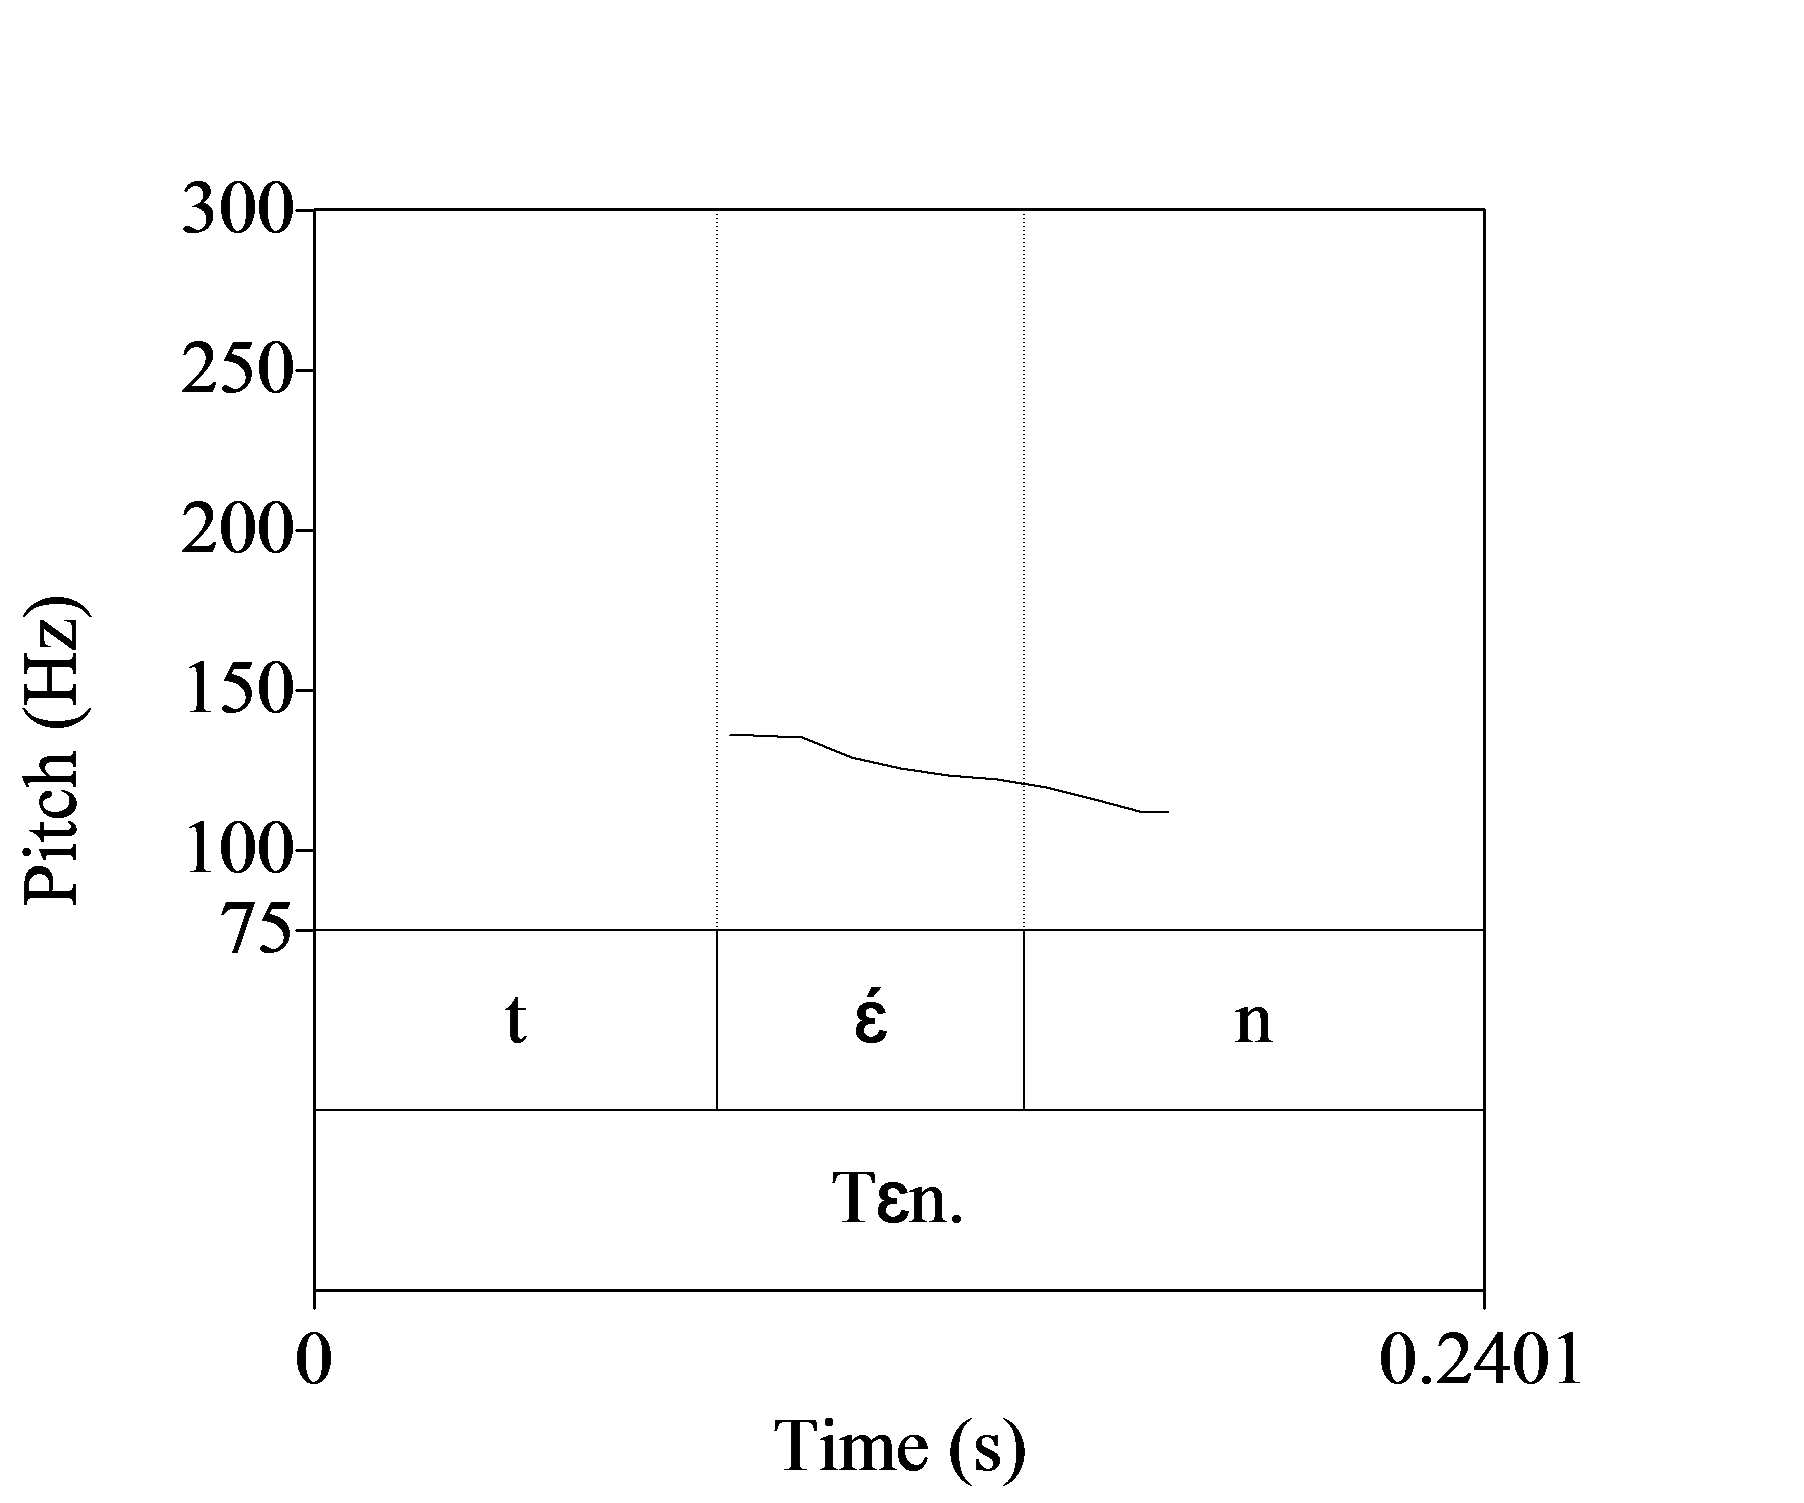
\includegraphics[width=.44\textwidth]{figures/yakpomod-img3.png}
	\label{fig:key:3.1}
\end{figure}
\ea\label{ex:key:43}
\gll Tɛ́n.\\
\textsc{hl\%}\\
\glt  ‘Time’
\z
%}
%\end{minipage}

%\begin{minipage}{.45\textwidth}
%\parbox{.45\textwidth}{
\begin{figure}
	\caption{Citation form of \textstyleTablePichiZchn{tɔ́k}}
	\label{fig:key:3.2}
	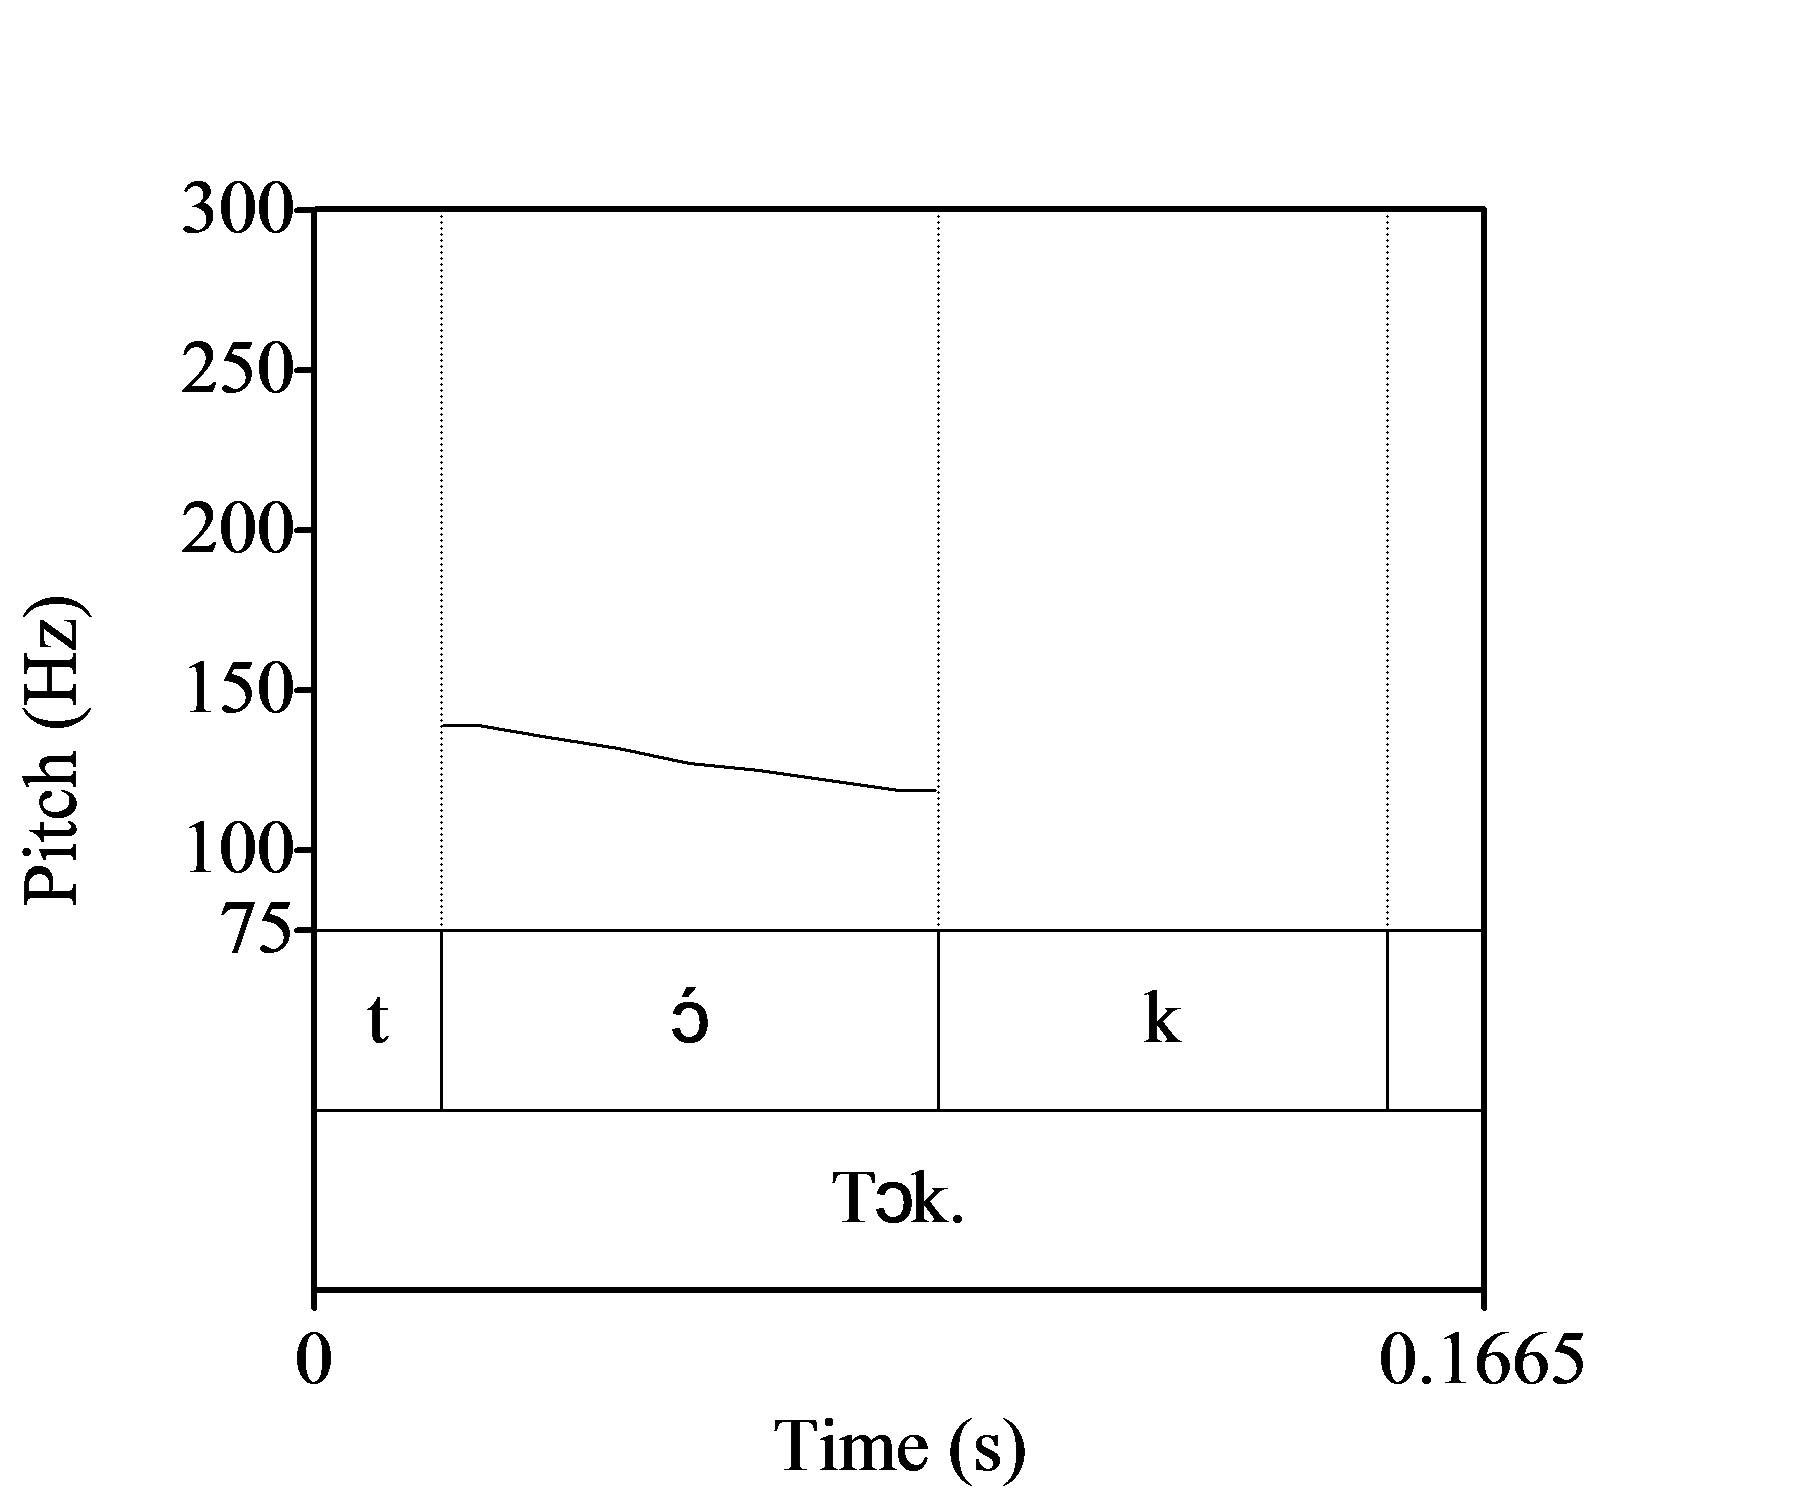
\includegraphics[width=.44\textwidth]{figures/yakpomod-img4.png}
\end{figure}
\ea\label{ex:key:44}
\gll Tɔ́k.\\
\textsc{hl\%}\\
\glt ‘Talk’
\z
%}
%\end{minipage}

When the utterance-final word is a light (vowel-final) monosyllable, the vowel may be lengthened, sometimes up to two beats. I assume that the lengthening of light monosyllables is caused by the metric preference of Pichi for footed tonal domains within the word boundary. Heavy monosyllables with a final non-tone-bearing segment like \textit{tɔ́k} ‘talk’ block the creation of footed domains in utterance-final position. But light syllables leave room for this option. The vowels of the light monosyllables in the following two figures have been lengthened in order to accommodate the HL contour consisting of the lexical H tone of the monosyllable and the declarative L\% boundary tone: 

\begin{figure}
\caption{Citation form of \textstyleTablePichiZchn{só}}
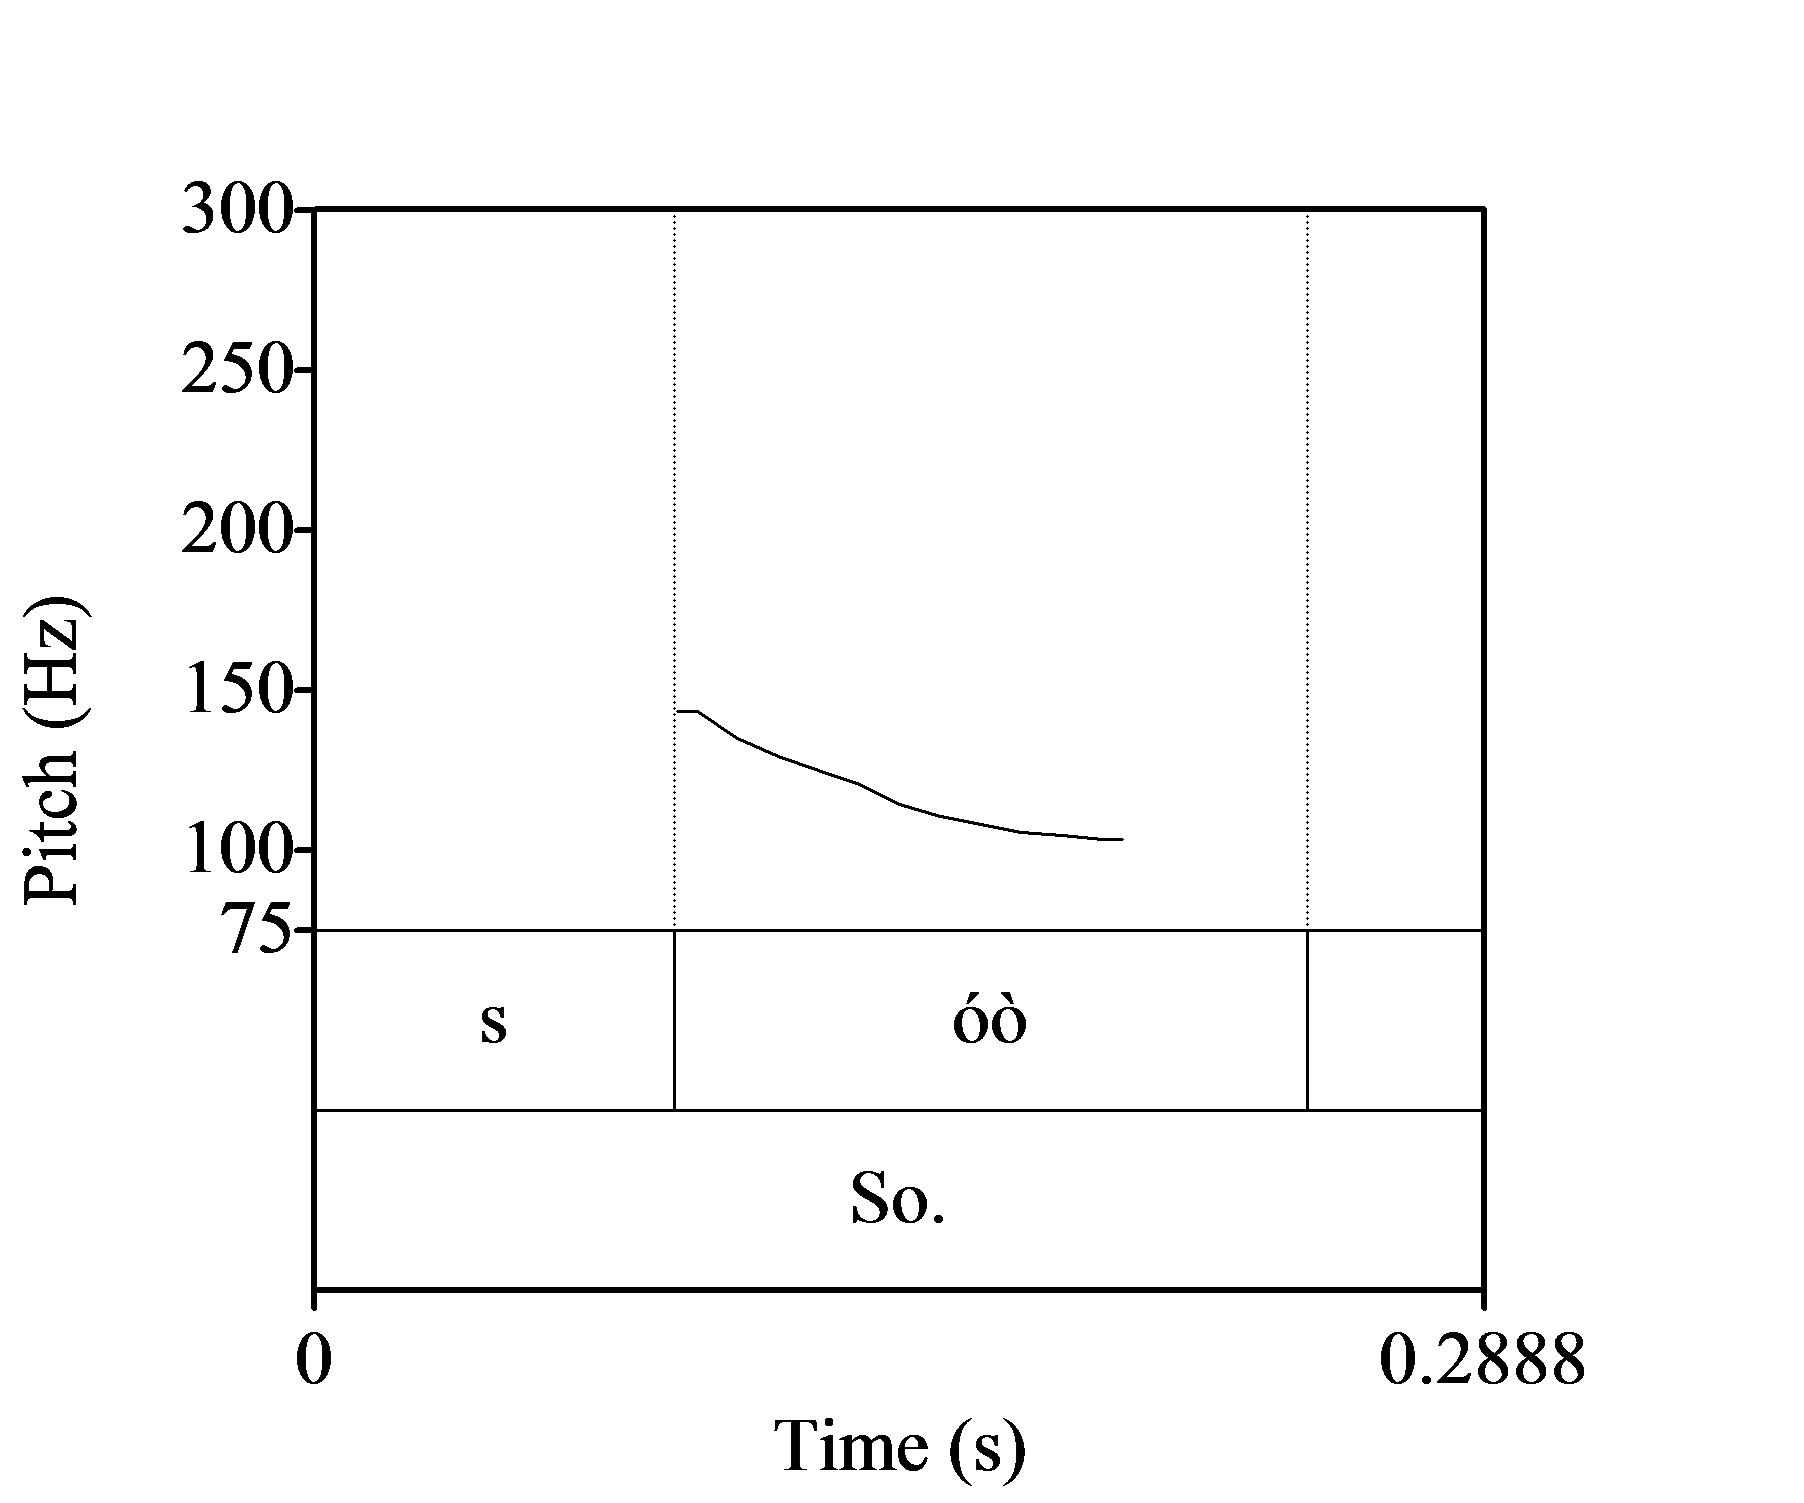
\includegraphics[height=.3\textheight]{figures/yakpomod-img5.png}
\label{fig:key:3.3}
\end{figure}

\begin{figure}
\caption{Citation form of \textstyleTablePichiZchn{dé}}
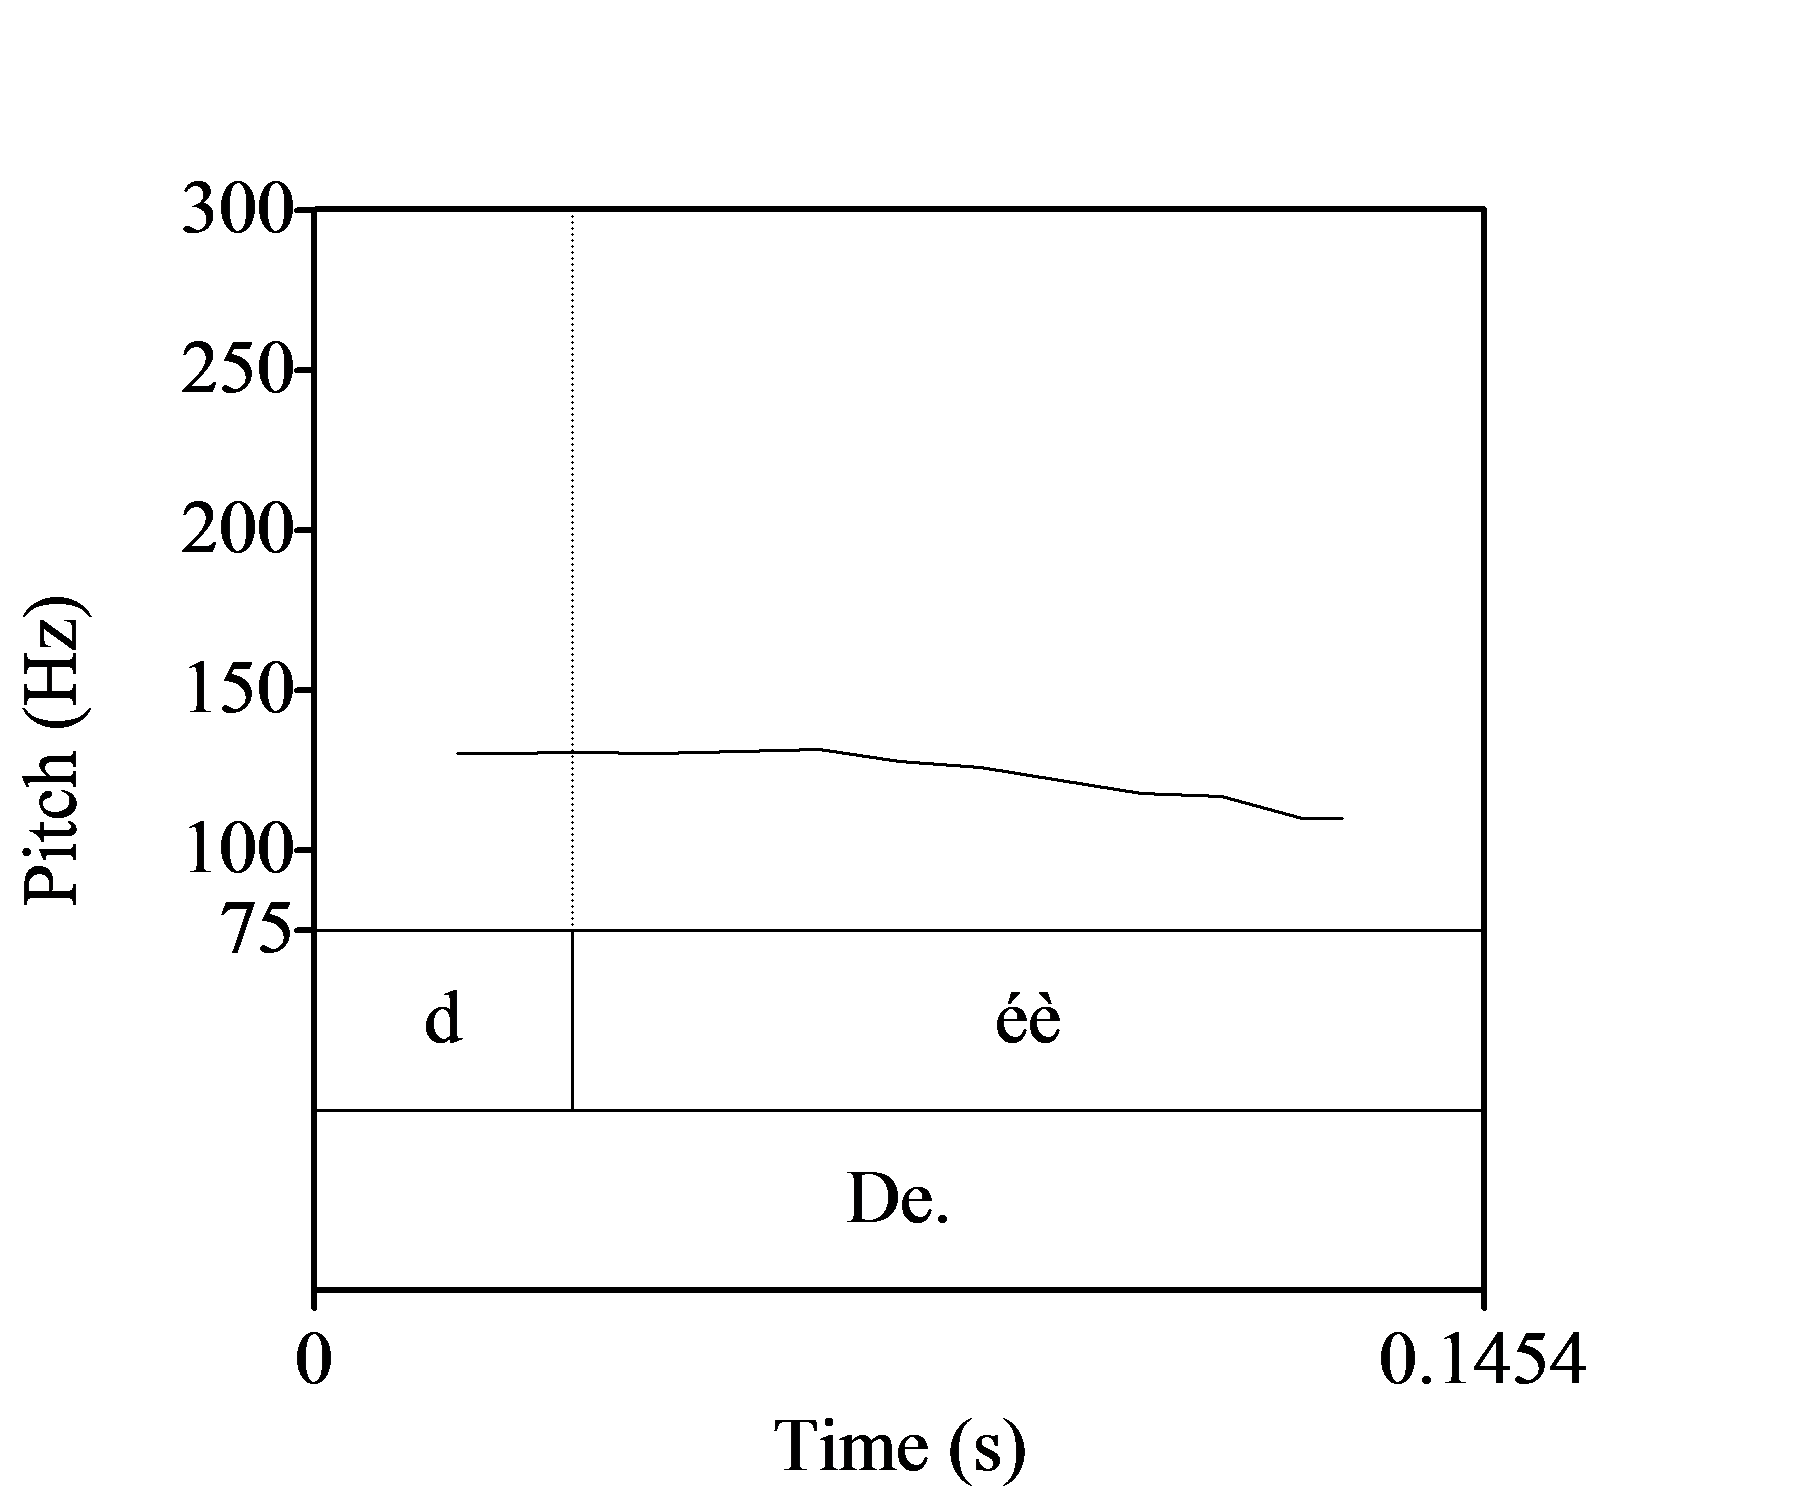
\includegraphics[height=.3\textheight]{figures/yakpomod-img6.png}
\label{fig:key:3.4} 
\end{figure} 

\ea\label{ex:key:45}
\gll      S\textstylePichiexamplebold{ó}.\\
\textsc{h}\textstylePichiexamplebold{\textsc{l\%}}\\
\glt ‘Like that.’
\z
\ea\label{ex:key:46}
\gll    D\textstylePichiexamplebold{é}.\\
\textsc{h}\textstylePichiexamplebold{\textsc{l\%}}\\
\glt ‘There.’
\z

\subsection{Distinctive tones}

Pichi contrasts two level tones, a high tone (H) and a low tone (L). H tone is the more active tone in tonal processes. H rather than L participates in tone spreading and is more active in pitch register expansion. Contour tones do not constitute tonemes in their own right. Instead, they result from the succession of a lexical tone and a polar floating tone over a single tone-bearing unit (cf. \sectref{sec:3.2.2}). 

\figref{fig:key:3.5} and \figref{fig:key:3.6} below present the pitch trace and segmentation of the two words \textit{hasis} /H.L/ ‘ashes’ and \textit{dɔtí} /L.H/ ‘be dirty’ said in isolation:

\begin{figure}
\caption{H.L pattern}
\label{fig:key:3.5}
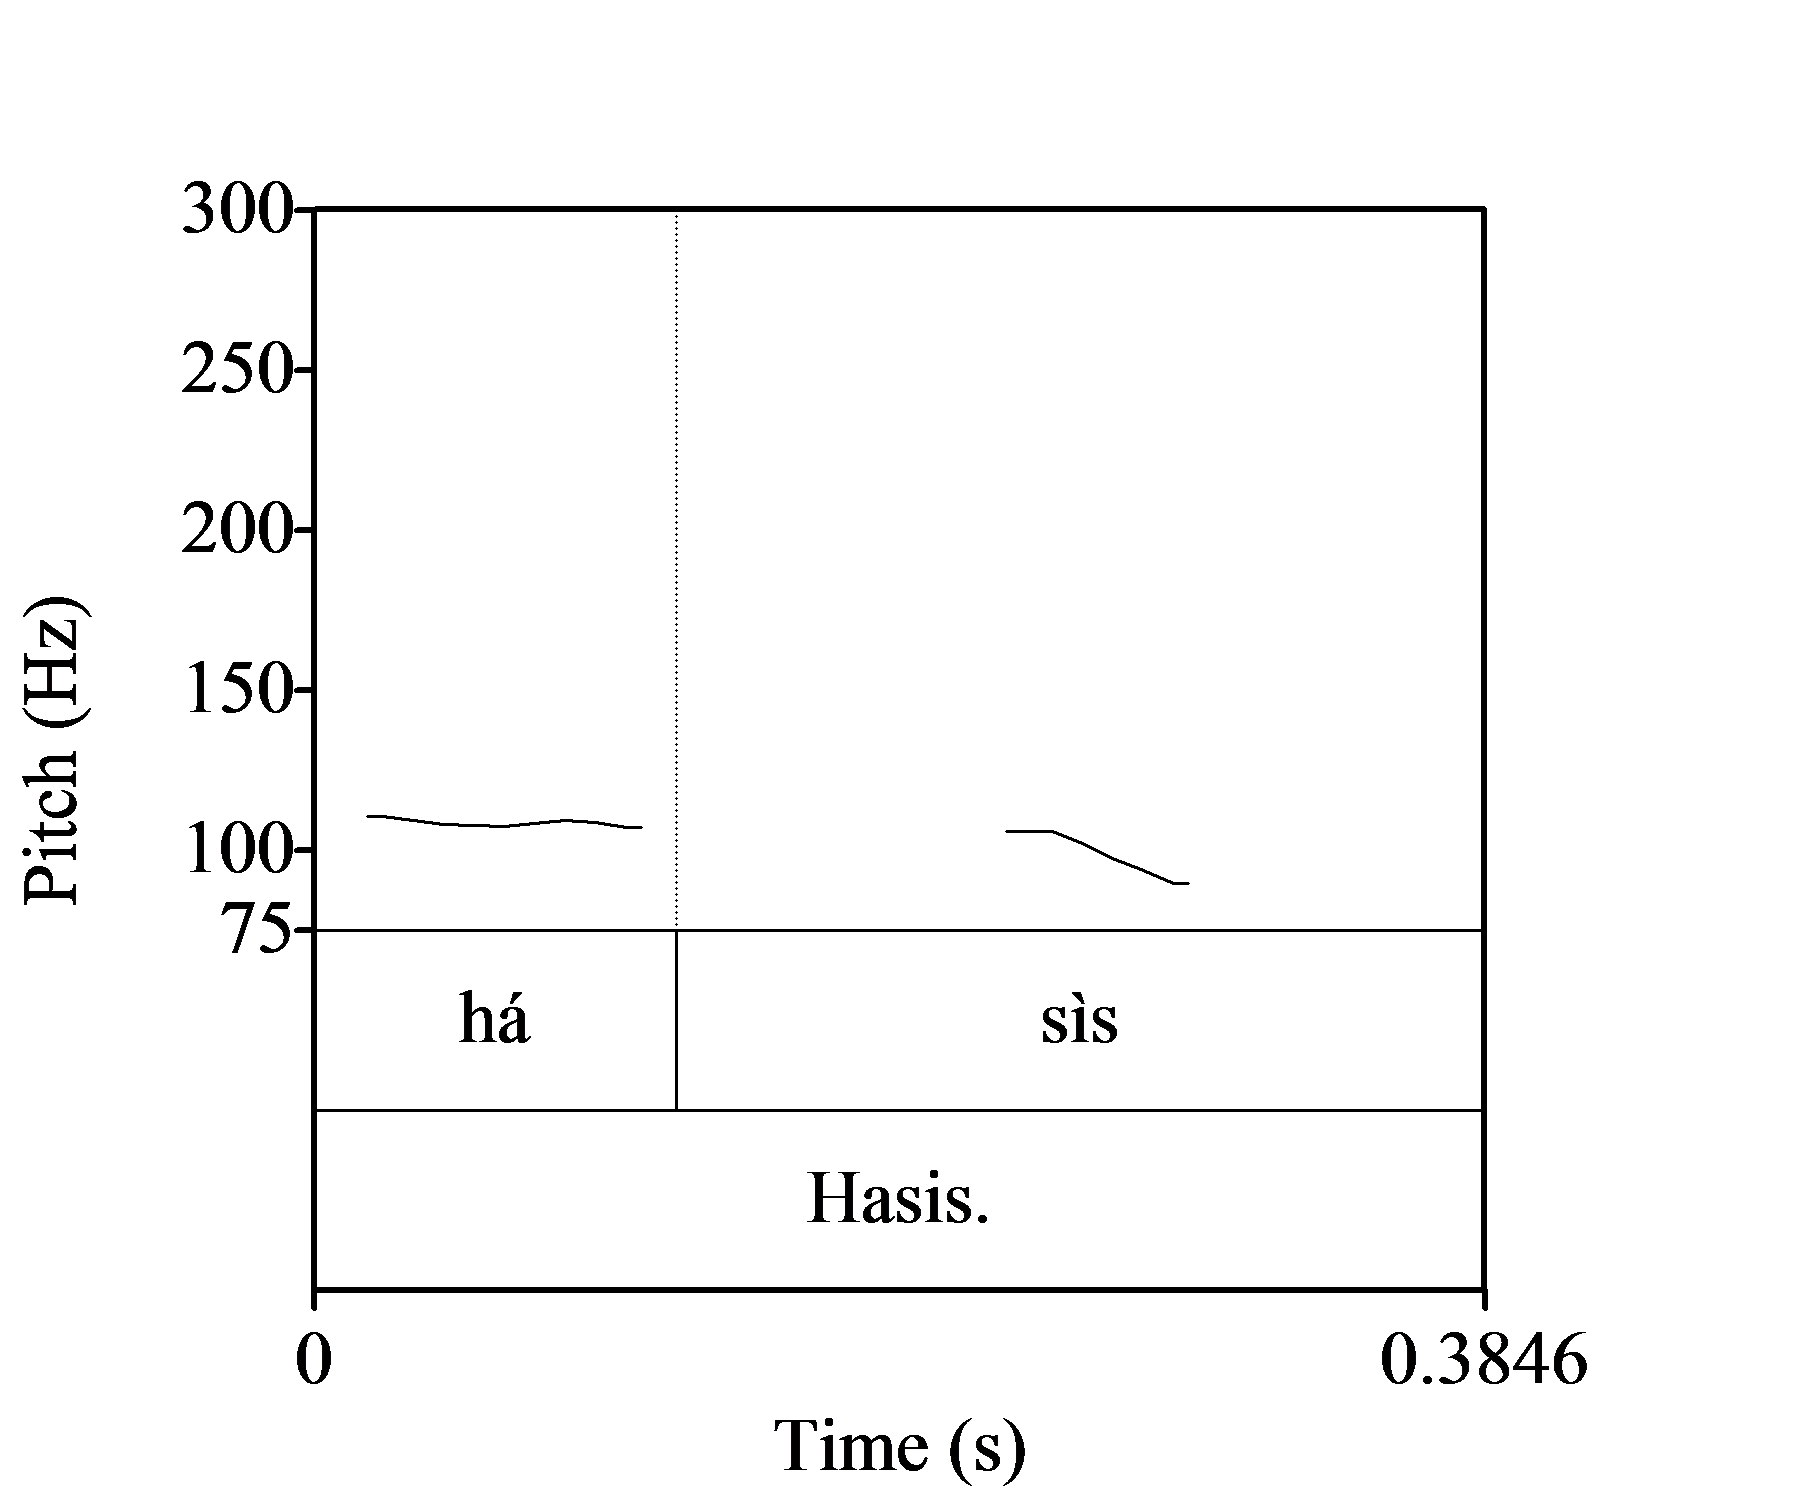
\includegraphics[height=.3\textheight]{figures/yakpomod-img7.png}
\end{figure}

\begin{figure}
\caption{L.H pattern}
\label{fig:key:3.6}  
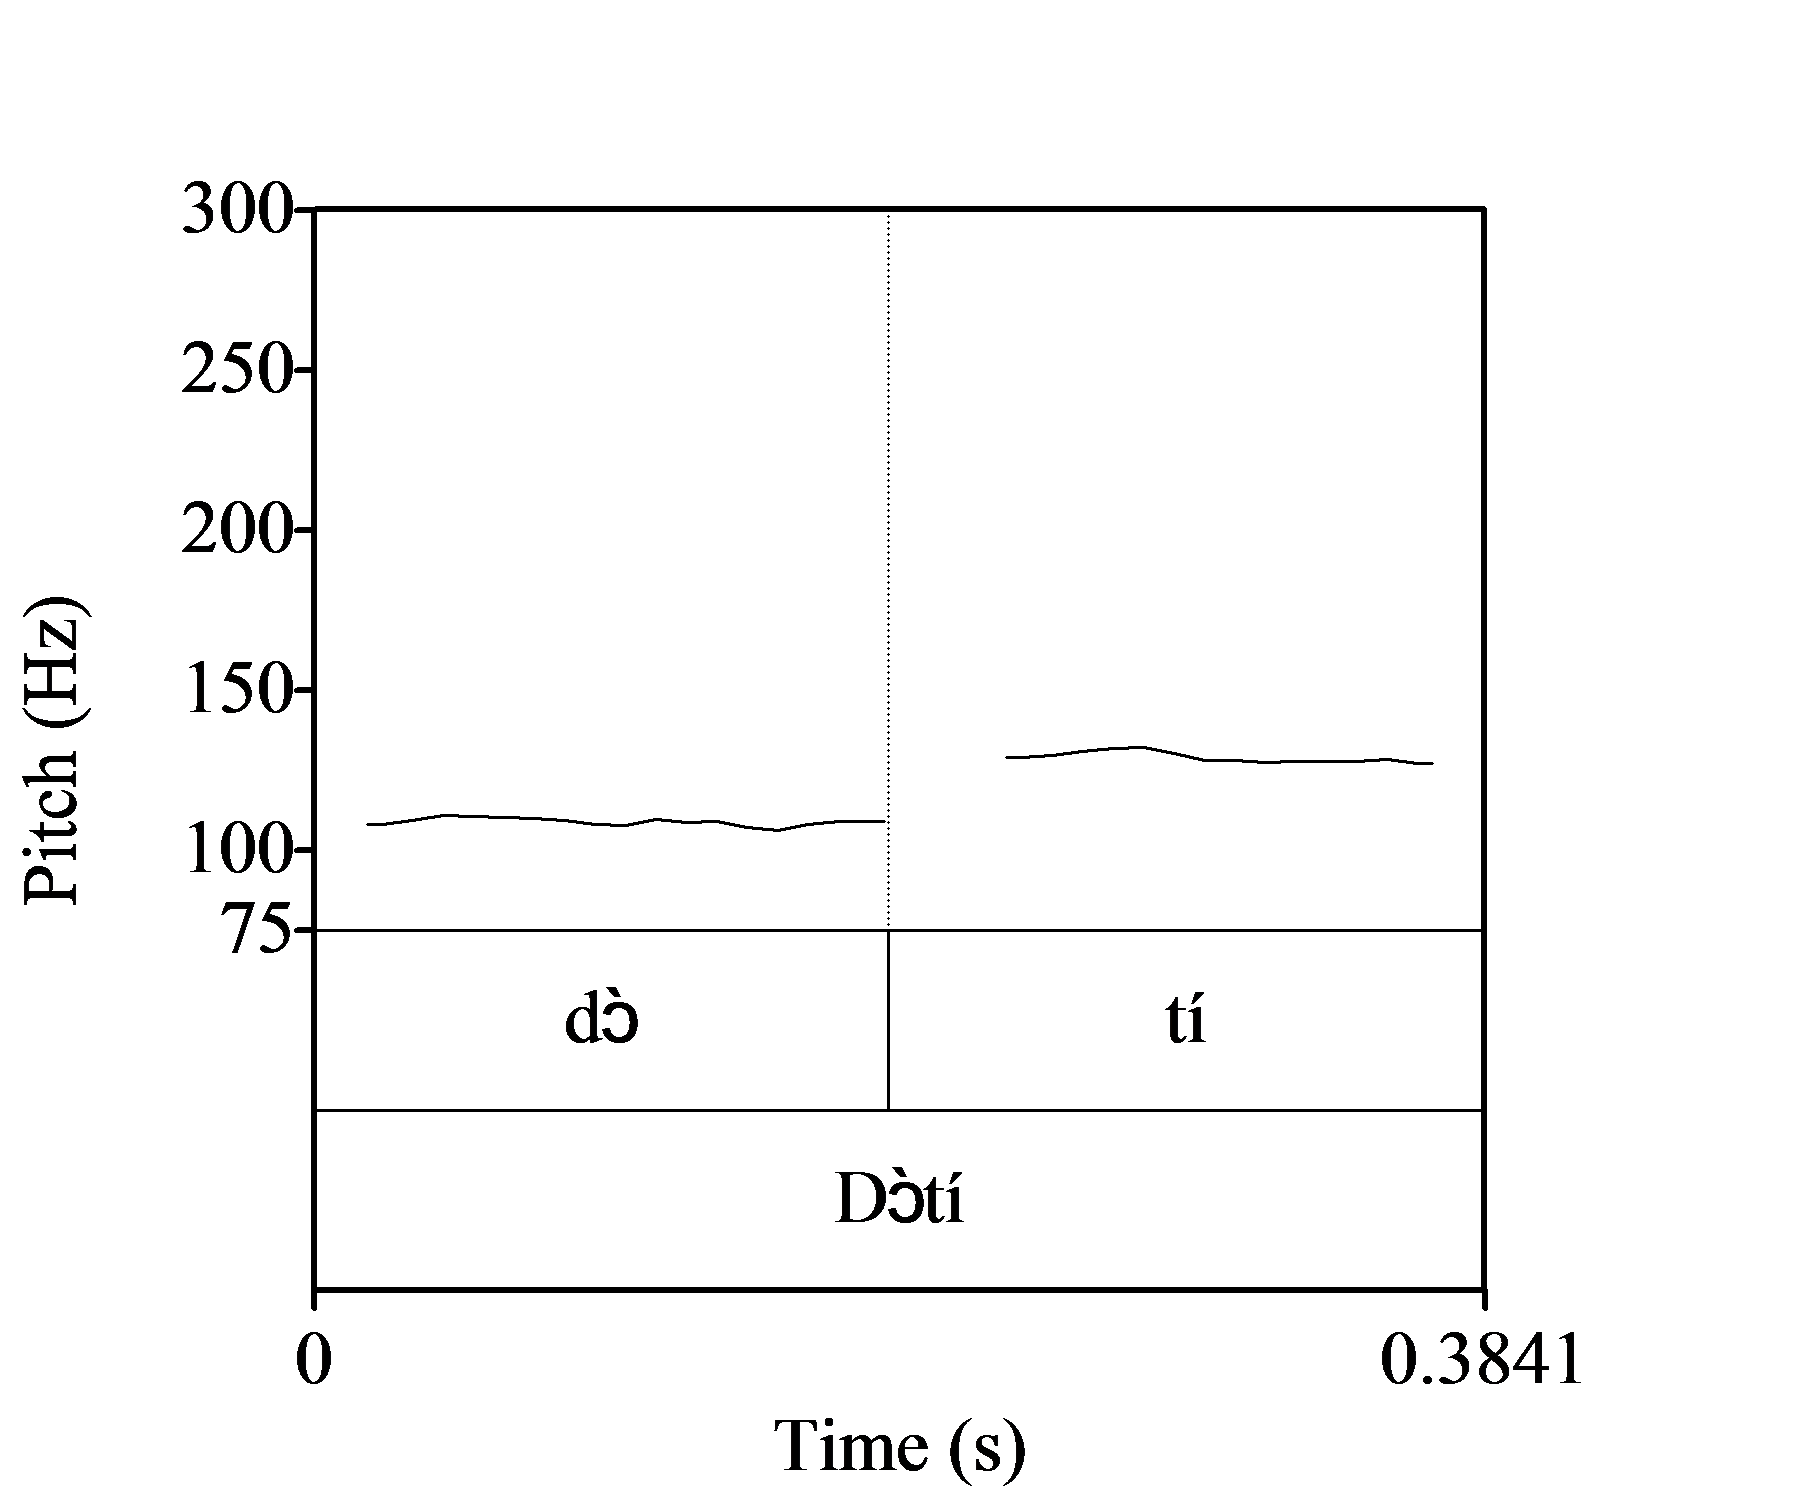
\includegraphics[height=.3\textheight]{figures/yakpomod-img8.png}
\end{figure}

The two words above represent the tone patterns of the two most frequent tone classes of Pichi (cf. \tabref{tab:key:3.1}). The mean pitch on the L-toned syllable of \textit{dɔtí} is 109.17~Hz, that of the H-toned syllable 129.27~Hz. Hence, the difference in pitch between the H- and L-level tones amounts to 20.1~Hz. With \textit{hásis}, the mean pitch of the H tone is 108.59~Hz, while the mean L tone stands at 99.72~Hz. The difference in mean pitch between H and L therefore stands at 8.87~Hz. This difference is just about half of that between L and H in \textit{dɔtí}:

%%please move \begin{table} just above \begin{tabular
\begin{table}
\caption{Pitch values}
\label{tab:key:3.1}

\begin{tabularx}{.5\textwidth}{Xrr}
\lsptoprule
Hertz & \itshape dɔtí & \itshape hásis\\
\midrule
Mean Hz of H    & 129.27 & 108.59\\
Mean Hz of L    & 109.17 & 99.72\\
Highest Hz of H & 132.20 & 110.33\\
Lowest Hz of H  & 127.26 & 107.35\\
Highest Hz of L & 110.78 & 105.83\\
Lowest Hz of L  & 107.47 & 93.50\\
\lspbottomrule
\end{tabularx}
\end{table}
The relatively small difference in mean pitch between the syllables of \textit{hásis} arises due to the fact that the H tone over the first syllable is carried over into the first half of the following L-toned syllable. In contrast, the L tone of the first syllable of \textit{dɔtí} shows no signs of rightward spreading. 


Words may bear a single or more H or L tones. Compare the pitch traces of the utterance-final tonal words nyɔ́ní ‘ant’ and Bata ‘Fang’ in the collocations lɛ́k nyɔ́ní ‘like ants’ and tɔ́k Bata ‘speak Fang’ below:


\begin{figure}
\caption{H.H pattern} 
\label{fig:key:3.7}
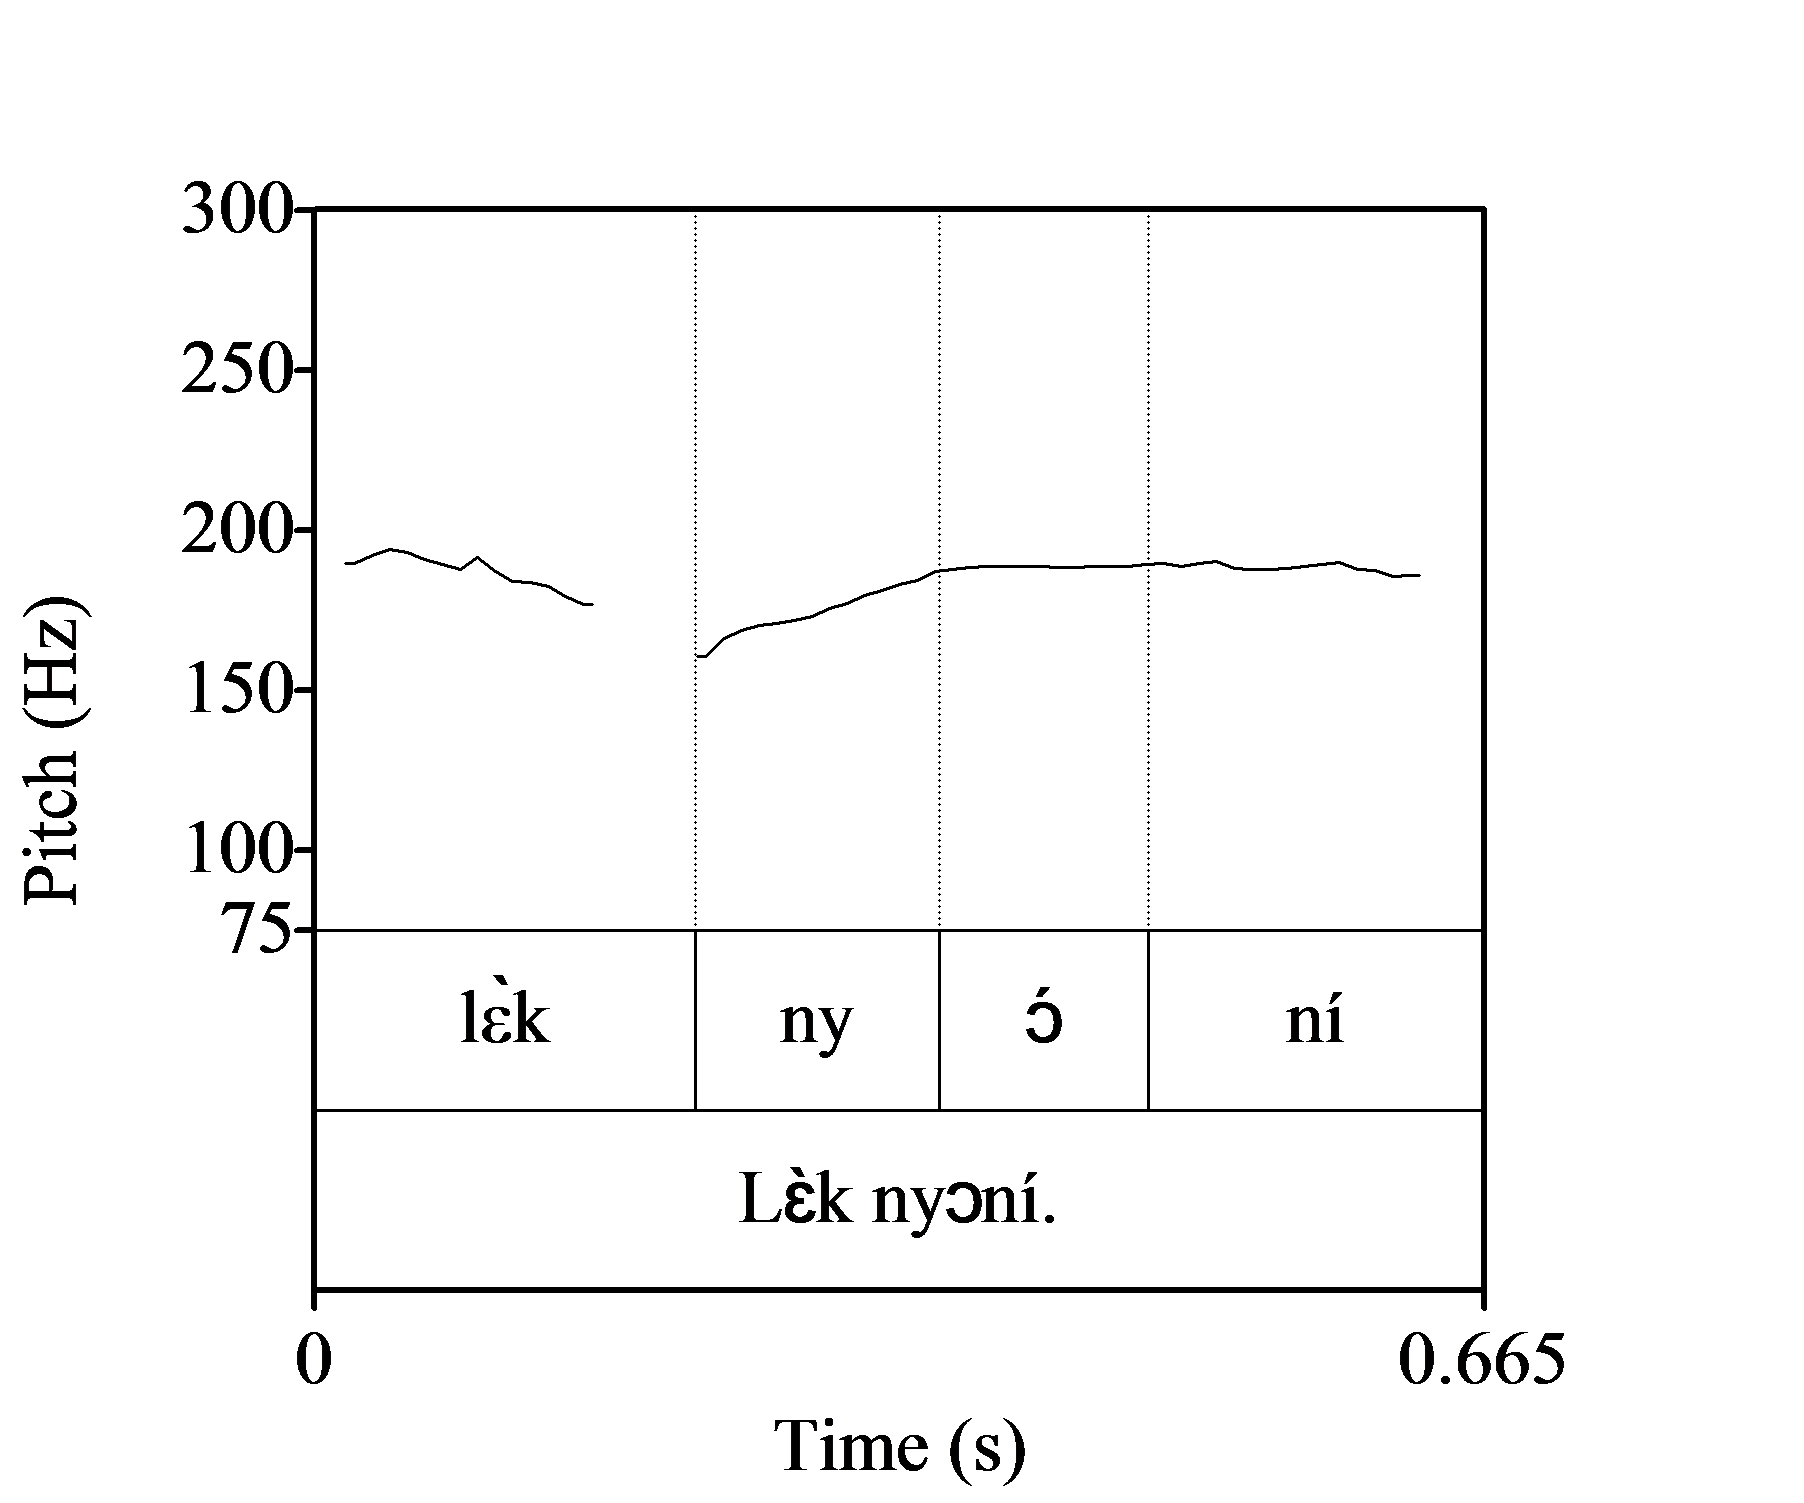
\includegraphics[height=.3\textheight]{figures/yakpomod-img9.png}
\end{figure}

\begin{figure}
\label{fig:key:3.8}
\caption{L.L pattern}
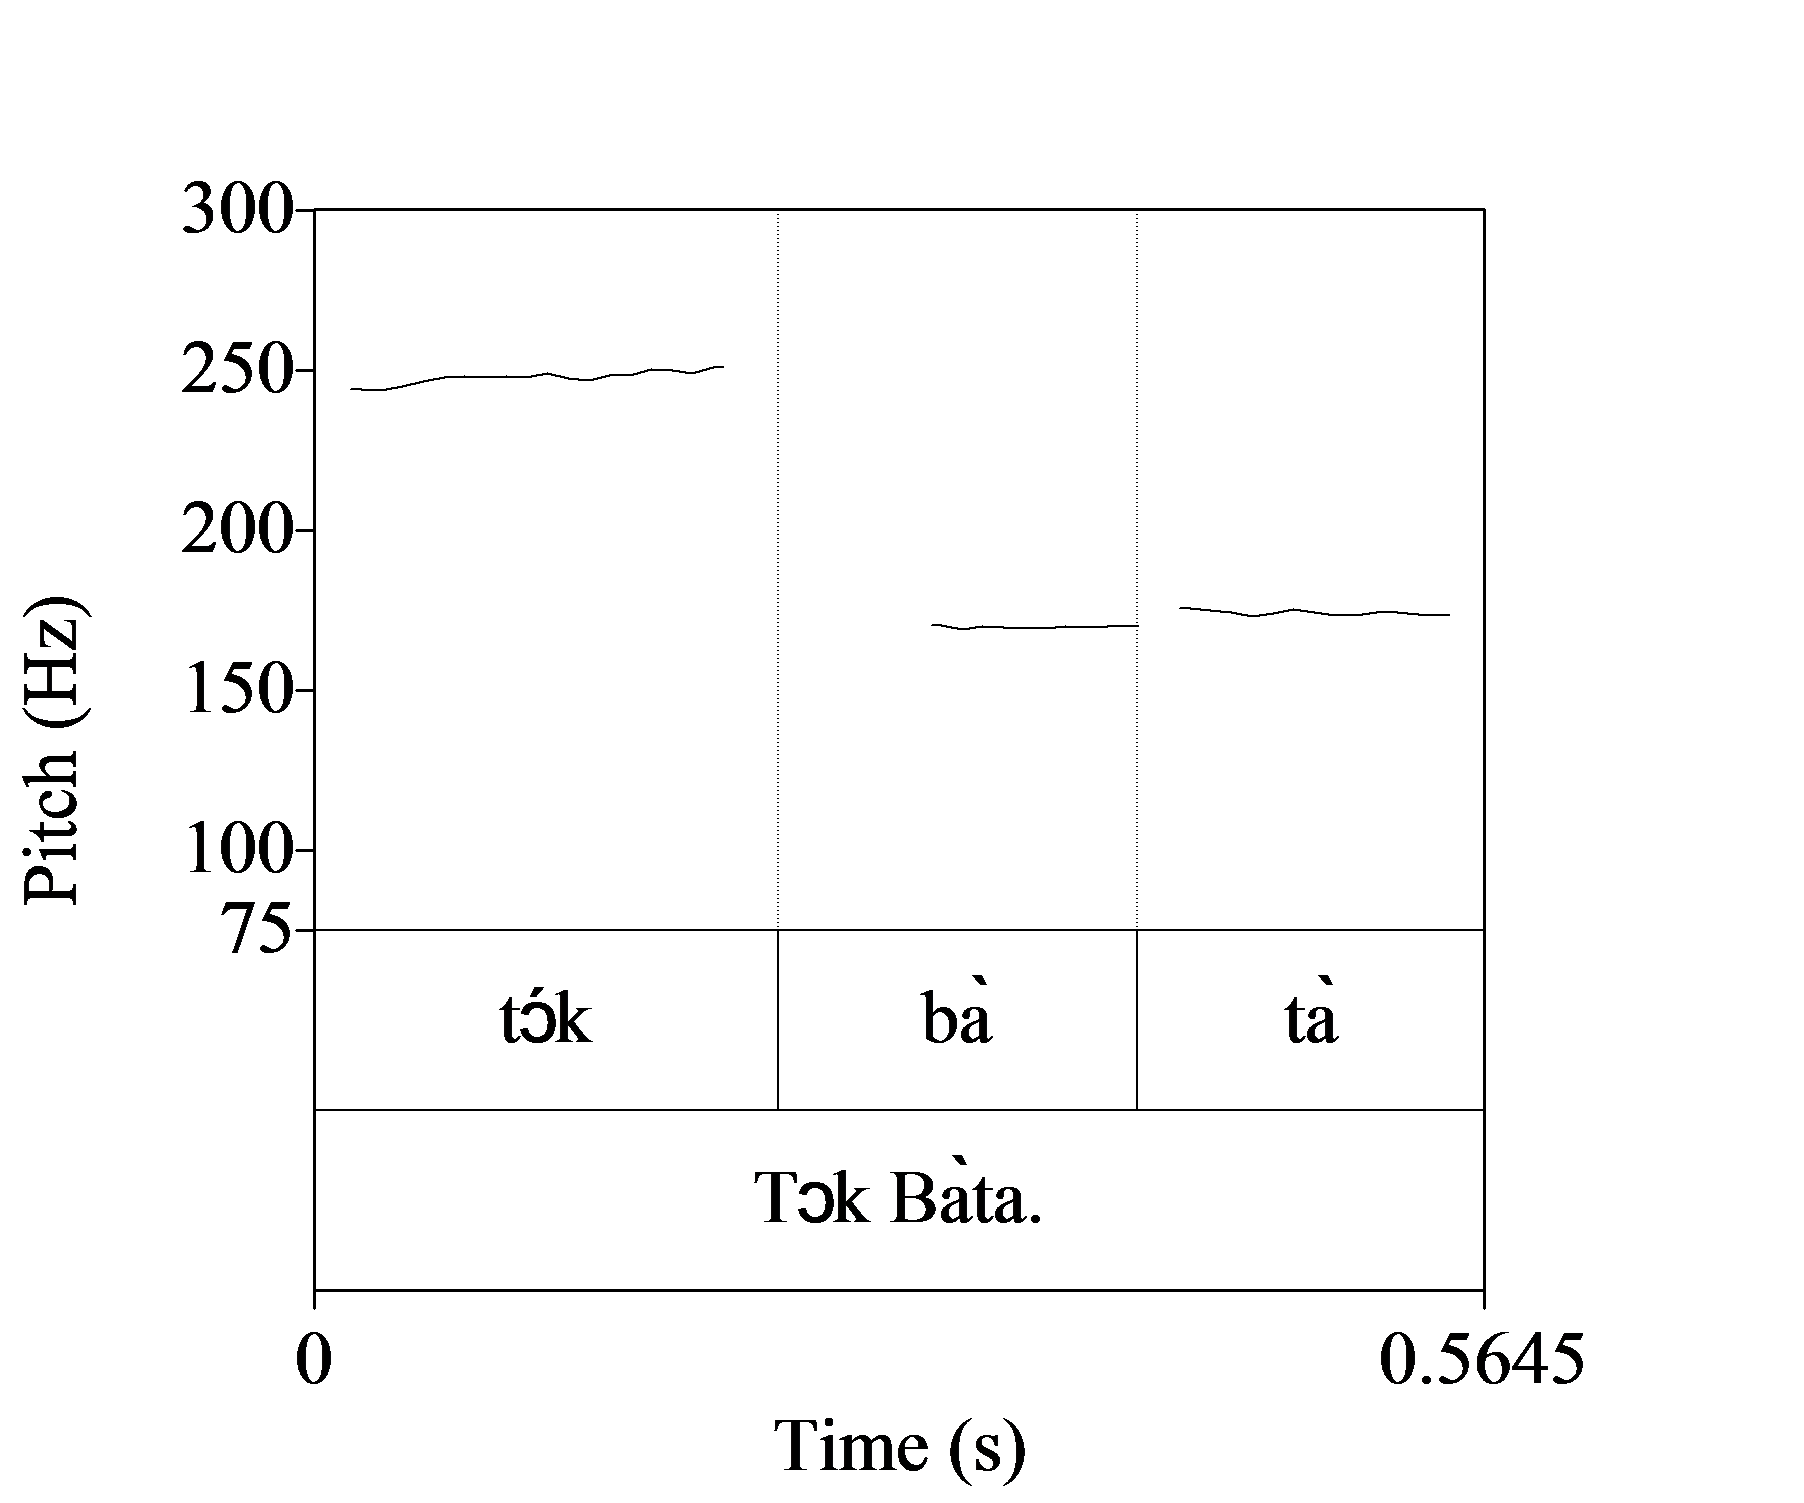
\includegraphics[height=.3\textheight]{figures/yakpomod-img10.png}
\end{figure}

Equatoguinean Spanish has been analysed as a tone language, in which the lexical stress characteristic of Spanish has been converted to lexical tone due to contact with the tone languages of Equatorial Guinea (\citealt{Lipski2015,SteienYakpo2017}). Words code-switched or borrowed from Equatoguinean Spanish are therefore specified for lexical tone just like Pichi words. 


The two tables below feature the utterance-final Spanish words \textit{abril} ‘April’ and \textit{nigeriano} ‘Nigerian’, the latter in the collocation \textit{na} \textit{nigeriano} ‘\textsc{foc} Nigerian’ \textit{=} ‘He is a Nigerian’. The pitch configurations over these two words conforms to those of Pichi words with a word-final (\figref{fig:key:3.9}) and a penultimate (\figref{fig:key:3.10}) H tone, respectively: 


\begin{figure}
\caption{Pitch over Spanish \textstyleTablePichiZchn{abril}}
\label{fig:key:3.9}
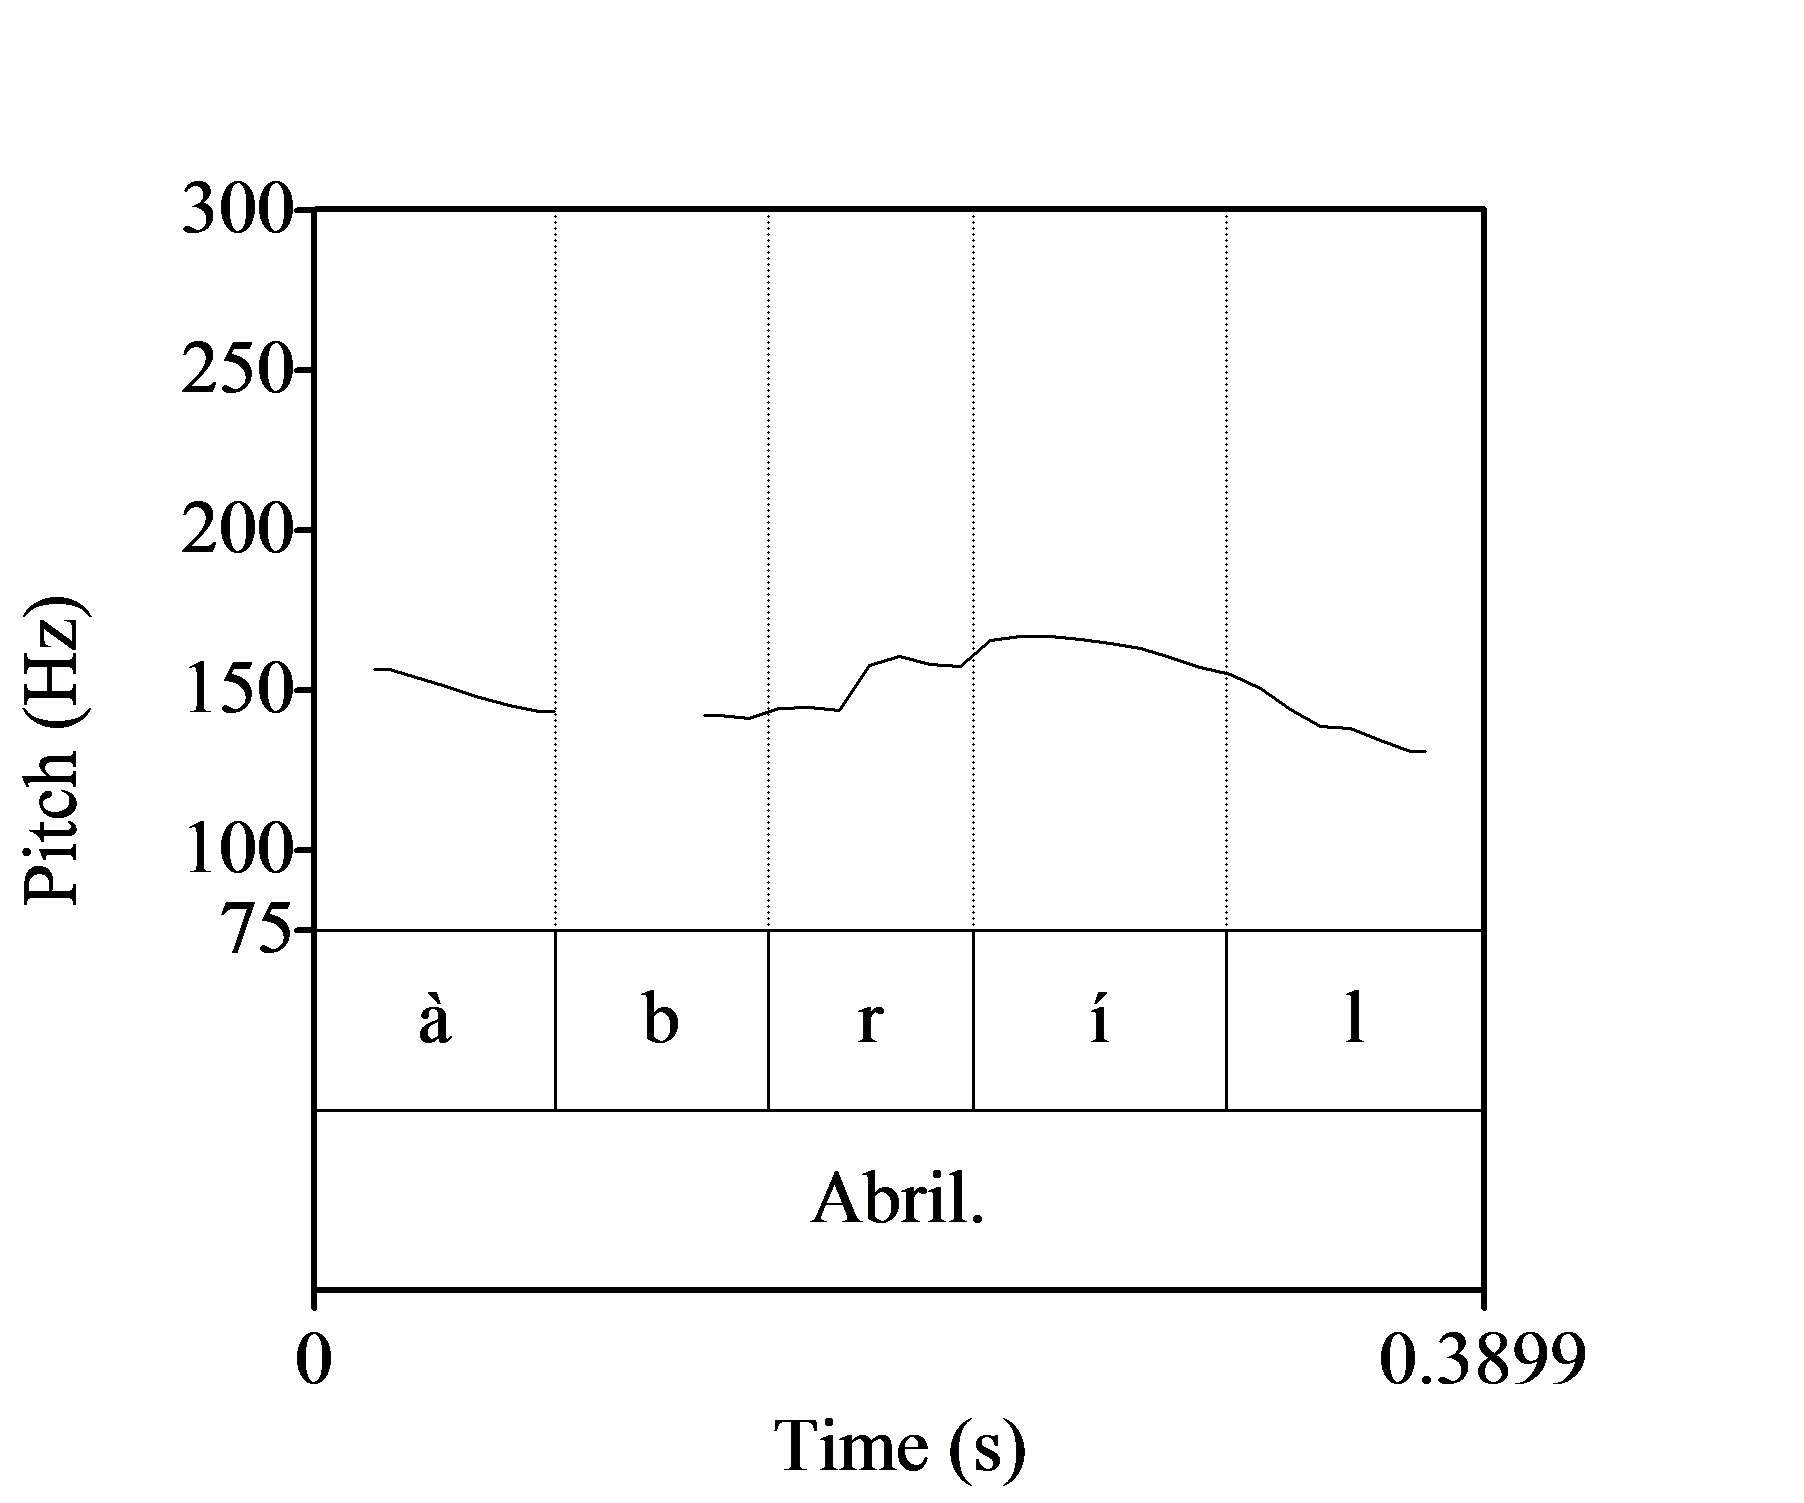
\includegraphics[height=.3\textheight]{figures/yakpomod-img11.png}
\end{figure}

\begin{figure}
\caption{Pitch over Spanish \textit{nigeriano}}
\label{fig:key:3.10} 
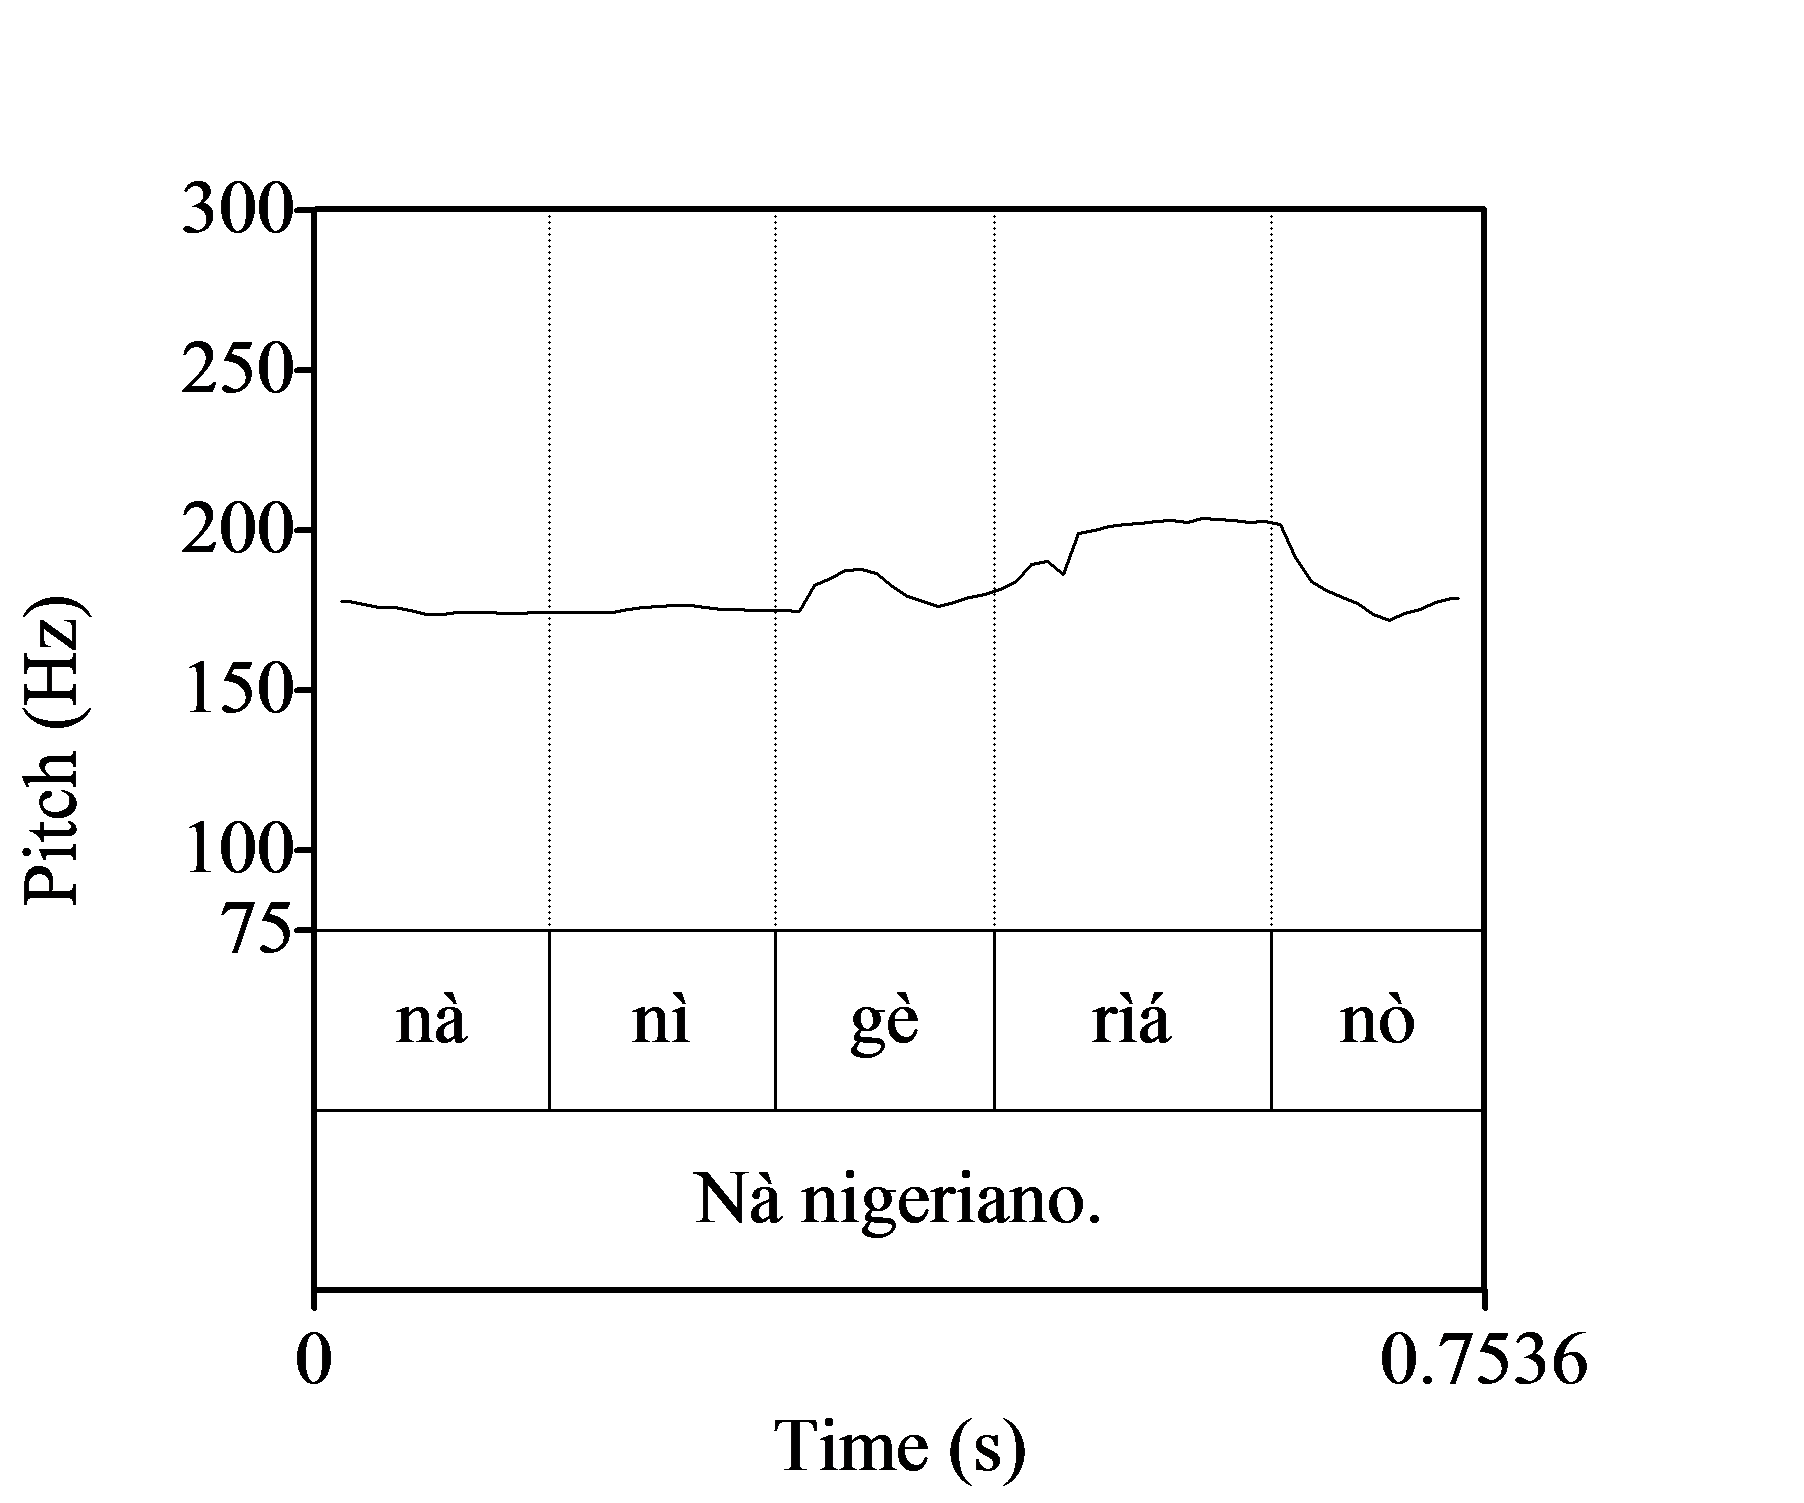
\includegraphics[height=.3\textheight]{figures/yakpomod-img12.png}
\end{figure}

\subsection{Lexical and morphological tone}

A small number of monosyllabic roots are distinguished from each other by pitch alone. The list in \REF{ex:key:47} contains most words in the corpus to which this applies. In conformity with a general pattern, (more) functional words are L-toned, while the corresponding content words are H-toned: 

\eabox{\label{ex:key:47}
\begin{tabularx}{\textwidth}{ll ll}
L tone &  & H tone & \\
\itshape bay & ‘by’ & \itshape báy & ‘buy’\\
\itshape bɔt & ‘but’ & \itshape bɔ́t & ‘hit with the head’\\
\itshape de & ‘\textsc{ipfv}’ & \itshape dé & ‘day; there’\\
\itshape di & ‘\textsc{def}’ & \itshape dí & ‘this’\\
\itshape lɛk & ‘like’ & \itshape lɛ́k & ‘(to) like’\\
\itshape so & ‘so’ & \itshape só & ‘like this; sew; show’\\
\itshape wet & ‘with’ & \itshape wét & ‘wait’\\
\end{tabularx}
}

However, there are also numerous homophones, which can neither be distinguished segmentally, nor by their pitch properties. The following list contains most homophones in the corpus: 

\eabox{\label{ex:key:48}
\begin{tabularx}{\textwidth}{ll ll}
\multicolumn{2}{l}{Homophones} &  & \\
\itshape dé & ‘day; there; \textsc{be.loc}’ & \itshape líf & ‘leaf; live’\\
\itshape an & ‘\textsc{3sg.obj}; and’ & \itshape lɔ́s & ‘loose; louse’\\
\itshape día & ‘deer; expensive’ & \itshape na & \textsc{‘foc;} \textsc{loc’}\\
\itshape bia & ‘beer; bear’ & \itshape nó & ‘know; \textsc{neg’}\\
\itshape bló & ‘blow; relax’ & \itshape nyús & ‘news; use’\\
\itshape fɔ́l & ‘fowl; to rain’ & \itshape pía & ‘avocado; pair’\\
\itshape fɔ́s & ‘first; force’ & \itshape ráyt & ‘right; write’\\
\itshape fíl & ‘feel; field’ & \itshape rɛ́s & ‘rest; rice’\\
\itshape hát & ‘heart; to hurt’ & \itshape rɔ́n & ‘run; be wrong’\\
\itshape hía & ‘hear; here; year; hair’ & \itshape só & ‘sew; show’\\
\itshape hól & ‘hole; hold; whole’ & \itshape sɔ́t & ‘shirt; short’\\
\itshape (h)ɔ́t & ‘extinguish; hot’ & \itshape tɔ́n & ‘town; turn’\\
\itshape klós & ‘clothing’ & \itshape tú & ‘too (much); two’\\
\itshape kɔ́s & ‘cost; (to) insult’ & \itshape wé & ‘way; \textsc{sub’}\\
\itshape lɛ́f & ‘leave; left’ & \itshape wích & ‘bewitch; which’\\
\end{tabularx}
}
Morphological tone is employed in the personal pronoun paradigm in order to distinguish morphologically different forms of the same lexeme from one another (e.g. mi \textsc{‘1sg.poss’} – mí \textsc{‘1sg.indp’}, dɛn ‘\textsc{3pl}’ – dɛ́n ‘\textsc{3pl.indp}’). Pichi also features a morphological tonal process (cf. \sectref{sec:3.2.4}). In addition, there are three items which have morphologically different forms, but presumably derive from a common etymon and are distinguished by pitch alone: de ‘ipfv’ – dé ‘be.\textsc{loc}’, di \textsc{‘def’} – dí ‘this’, go ‘pot’ – gó ‘go’). All low-toned monosyllabic roots are words with more or less grammatical functions, such as personal pronouns (e.g. a ‘\textsc{1sg.sbj}’), determiners (e.g. di ‘\textsc{def}’), TMA markers (e.g. bin ‘\textsc{pst}’, kin ‘\textsc{hab}’), clause linkers (e.g. ɛf ‘if’), or prepositions (e.g. pan ‘on’). Low-toned function words, except dependent personal pronouns, are listed in \REF{ex:key:49}:

\eabox{\label{ex:key:49}
\begin{tabularx}{\textwidth}{XXXXX}
\multicolumn{2}{l}{Low-toned function words} & \multicolumn{2}{c}{}\\
\itshape di & ‘\textsc{def}’ & \itshape lɛk(ɛ) & ‘like’\\
\itshape sɔn & ‘some, a’ & \itshape na & \textsc{‘loc;} \textsc{foc’}\\
\itshape bin & ‘\textsc{pst}’ & \itshape pan & ‘on’\\
\itshape de & ‘\textsc{ipfv}’ & \itshape to & ‘to’\\
\itshape go & ‘\textsc{pot}’ & \itshape wet & ‘with’\\
\itshape kin & ‘\textsc{hab}’ & \itshape an & ‘and’\\
\itshape mɔs & ‘\textsc{obl}’ & \itshape ɔ & ‘or’\\
\itshape bay & ‘by’ & \itshape ɛf(ɛ) & ‘if’\\
\itshape fɔ & ‘\textsc{prep}’ & \itshape bɔt & ‘but’\\
\itshape frɔn & ‘from’ & \itshape so & ‘so’\\
\end{tabularx}
}

There are, however, limits to this pattern of functional differenciation by tone. The monosyllabic roots \textit{dɔ́n} ‘down; done; \textsc{prf’}, \textit{kán} ‘come; \textsc{pfv’,} \textit{mék} ‘make; \textsc{sbjv}’, \textit{sé} ‘say; \textsc{quot’,} and \textit{wán} ‘one; a’ also have a more grammatical meaning besides their lexical one. Yet, their different functions are covered by segmentally and suprasegmentally identical forms. 


Pichi also exhibits one morphological tonal process. In compounds and morphological reduplication, the H tones over all non-final components are deleted and replaced by an L tone (cf. \sectref{sec:3.2.4}).


\subsection{Tone classes}\label{sec:3.1.3}

About 95 per cent of roots contained in my lexical data-base carry a single H tone over their only, penultimate, or final syllable. Other syllables in these words are L-toned. The remaining 5 per cent of roots feature diverse tone patterns with more than one H, or no H tone. Many (e.g. \textit{nyɔ́ní} ‘ant’ < Mende \textit{yɔ́ní} ‘red ant’) but not all (e.g. \textit{ápás} ‘after’ < English ‘half-past’) of these words originate from African languages or are monosyllabic function words with an L tone over their only syllable (cf. \REF{ex:key:49}, while words with a single H tone are mostly English-derived. This circumstance speaks to the fact that stress-to-tone conversion took place in the formation of the proto-language of Pichi, as in many other Afro-European creole and non-creole contact (e.g. \citealt{Berry1970,Criper1971,Criper-Friedman1990,Alleyne1980,GussenhovenUdofot2010,Steien2015}). 

\tabref{tab:key:3.2} below contains a listing of the tone classes of the simplex roots contained in the lexical data base of the corpus. (cf. \citealt{Faraclas1996,Good2004}, for pitch classes in Nigerian Pidgin and Saramaccan). A few examples are provided for each tone class. Not included in this table are ideophones\is{ideophones}, which feature a number of idiosyncratic tonal patterns and often involve lexicalised reduplication and triplication (cf. \sectref{sec:4.5.3} and \sectref{sec:12.1} for a detailed treatment).

Members of the monosyllabic L-toned tone class only contribute a total of nineteen roots and 2.5 per cent of the total in terms of individual entries and are hence listed as belonging to a minor tone class. The members of this class are, however, mostly function words that constitute the backbone of the grammatical system of Pichi: the personal pronouns \textit{a} ‘\textsc{1sg.sbj}’, \textit{e} ‘\textsc{3sg.sbj}’, \textit{=an} ‘\textsc{3sg.obj}’; the \textsc{TMA} markers \textit{de} ‘\textsc{ipfv}’, \textit{go} ‘\textsc{pot}’, \textit{bin} ‘\textsc{pst}’; the preposition \textit{fɔ} ‘\textsc{prep}’ and the homonymous forms \textit{na} ‘\textsc{loc}’ and \textit{na} ‘\textsc{foc}’ outrank any other root of the language in a frequency count. This makes this tone class perceptually as salient as the H and H.L tone classes. In contrast, the members of the other minor tone classes are each  composed of relatively few lexical words, which together make up 6 per cent of roots in the corpus. 


%%please move \begin{table} just above \begin{tabular
\begin{table}
\caption{Distribution of tone classes over types}
\label{tab:key:3.2}

\begin{tabularx}{\textwidth}{lXrr}
\lsptoprule

{{Tone classes}} & Examples & No. of items & \% of total\\
\midrule 
Major &  &  & \\
\midrule
  H & báy ‘buy’, áks ‘ask’, kɛ́r ‘carry; take’ & 413 & 54.1\\
  H.L & \textstyleTablePichiZchn{drɔ́ngo} ‘be dead drunk’, \textstyleTablePichiZchn{kɔ́mpin} ‘friend’ & 178 & 23.3\\
  L.H & \textstyleTablePichiZchn{bɔkú} ‘be much’, \textstyleTablePichiZchn{sabí} ‘know’, \textstyleTablePichiZchn{watá} ‘water’ & 107 & 14.0\\
\midrule 
{Subtotal} &  & {717} & {91.5}\\

\tablevspace
Minor &  &  & \\
\midrule 
  L & \textstyleTablePichiZchn{de} ‘\textsc{ipfv}’, \textstyleTablePichiZchn{go} ‘\textsc{pot}’, \textstyleTablePichiZchn{sɔn} ‘some, a’, \textstyleTablePichiZchn{fɔ} ‘\textsc{prep}’ & 19 & 2.5\\
  L.H.L & \textstyleTablePichiZchn{ɔspítul} ‘hospital’, \textstyleTablePichiZchn{wahála} ‘trouble’ & 14 & 1.8\\
  H.H & \textstyleTablePichiZchn{nyɔ́ní} ‘ant’, \textstyleTablePichiZchn{sóté} ‘until’, \textstyleTablePichiZchn{sósó} ‘only’, \textstyleTablePichiZchn{ápás} ‘after’ & 11 & 1.4\\
  L.L.H & \textstyleTablePichiZchn{ɔndastán} ‘understand’, \textstyleTablePichiZchn{prɔpatí} ‘property’ & 10 & 1.3\\
  H.L.L & kápinta ‘carpenter’, mɛ́rɛsin ‘medicine’ & 6 & 0.8\\
  L.H.H & \textstyleTablePichiZchn{okóbó} ‘impotent man’ & 3 & 0.4\\
  L.L & \textstyleTablePichiZchn{Bata} ‘\textsc{place’}, \textstyleTablePichiZchn{jɔmba} ‘affair’ & 2 & 0.3\\
\midrule 
{Subtotal} &  & {46} & {8.5}\\
\midrule 
Total &  & {763} & {100.0}\\
\lspbottomrule
\end{tabularx}
\end{table}

\tabref{tab:key:3.2} points to additional characteristics of the corpus. With 54.1 per cent, about half the roots are H-toned monosyllables. Another 25.2 per cent are polysyllabic roots with an H tone over the penultimate syllable (of which a mere 1.8 per cent have more than two syllables). Together, these two groups constitute an overwhelming majority of sec:79.3 per cent of all roots. An additional 15.3 per cent bear an H tone over the final syllable. Most roots in the corpus, namely 94.6 per cent, therefore carry an H tone over the only syllable, the penultimate syllable, or the final syllable.

It should also be mentioned that many of the Spanish items that find their way into code-mixed Pichi sentences bear a penultimate H tone in accordance with their original Spanish penultimate syllable stress. This holds in particular for the invariant \textsc{3sg} present insertion form of the Spanish verb (cf. \sectref{sec:13.2.2}). Spanish-origin items therefore align with the majority tone classes of Pichi.  


\section{Tonal processes}\label{sec:3.2}

Pitch changes conditioned by various factors may take place within a tonal domain. A tonal domain may be confined to the word, cut across a word boundary in specific phono-syntactic phrases, and involve a whole clause or sentence. The tonal processes attested in the data are described in \sectref{sec:3.2.1} to \sectref{sec:3.2.4}. A summary of these processes is given in \tabref{tab:key:3.3}:

%%please move \begin{table} just above \begin{tabular
\begin{table}
\caption{Tonal processes}
\label{tab:key:3.3}
\small
\begin{tabularx}{\textwidth}{lQQp{1.5cm}}
\lsptoprule
Process & Description & Conditioning factor & Tonal\newline  domain\\
\midrule 
Spreading & H spreads rightwards to L-toned syllable(s) & H spreads rightwards to L-toned syllables & (1) Word\\

\tablevspace
Floating & H is set afloat and docks onto a right-adjacent L-toned segment to form an HL contour tone & Vowel deletion and vowel merging & Adjacent function words\\

\tablevspace
Declination & H tones are progressively lowered across the utterance & (1) Downdrift\is{„downdrift}: an H is lowered by a preceding L
\newline 
(2)      Downstep\is{„downstep}: an H is lower in pitch than a left-adjacent H & Clause,\newline  sentence \\

\tablevspace
Deletion & The lexical tone is deleted and realised as L & (1) Derivation of compounds and reduplicants
\newline
(2)      Question boundary tone overrides lexical tone & (1) Phonological word
\newline 
(2)         Word\\
\lspbottomrule
\end{tabularx}
\end{table}

\subsection{Tone spreading}\label{sec:3.2.1}

H tones may spread to right-adjacent L-toned syllables within the word boundary. The H tone over the first syllable of \textit{prɔ́mis} ‘promise’ in \figref{fig:key:3.11} spreads to the second syllable: 

\begin{figure}
\caption{H tone spreading}
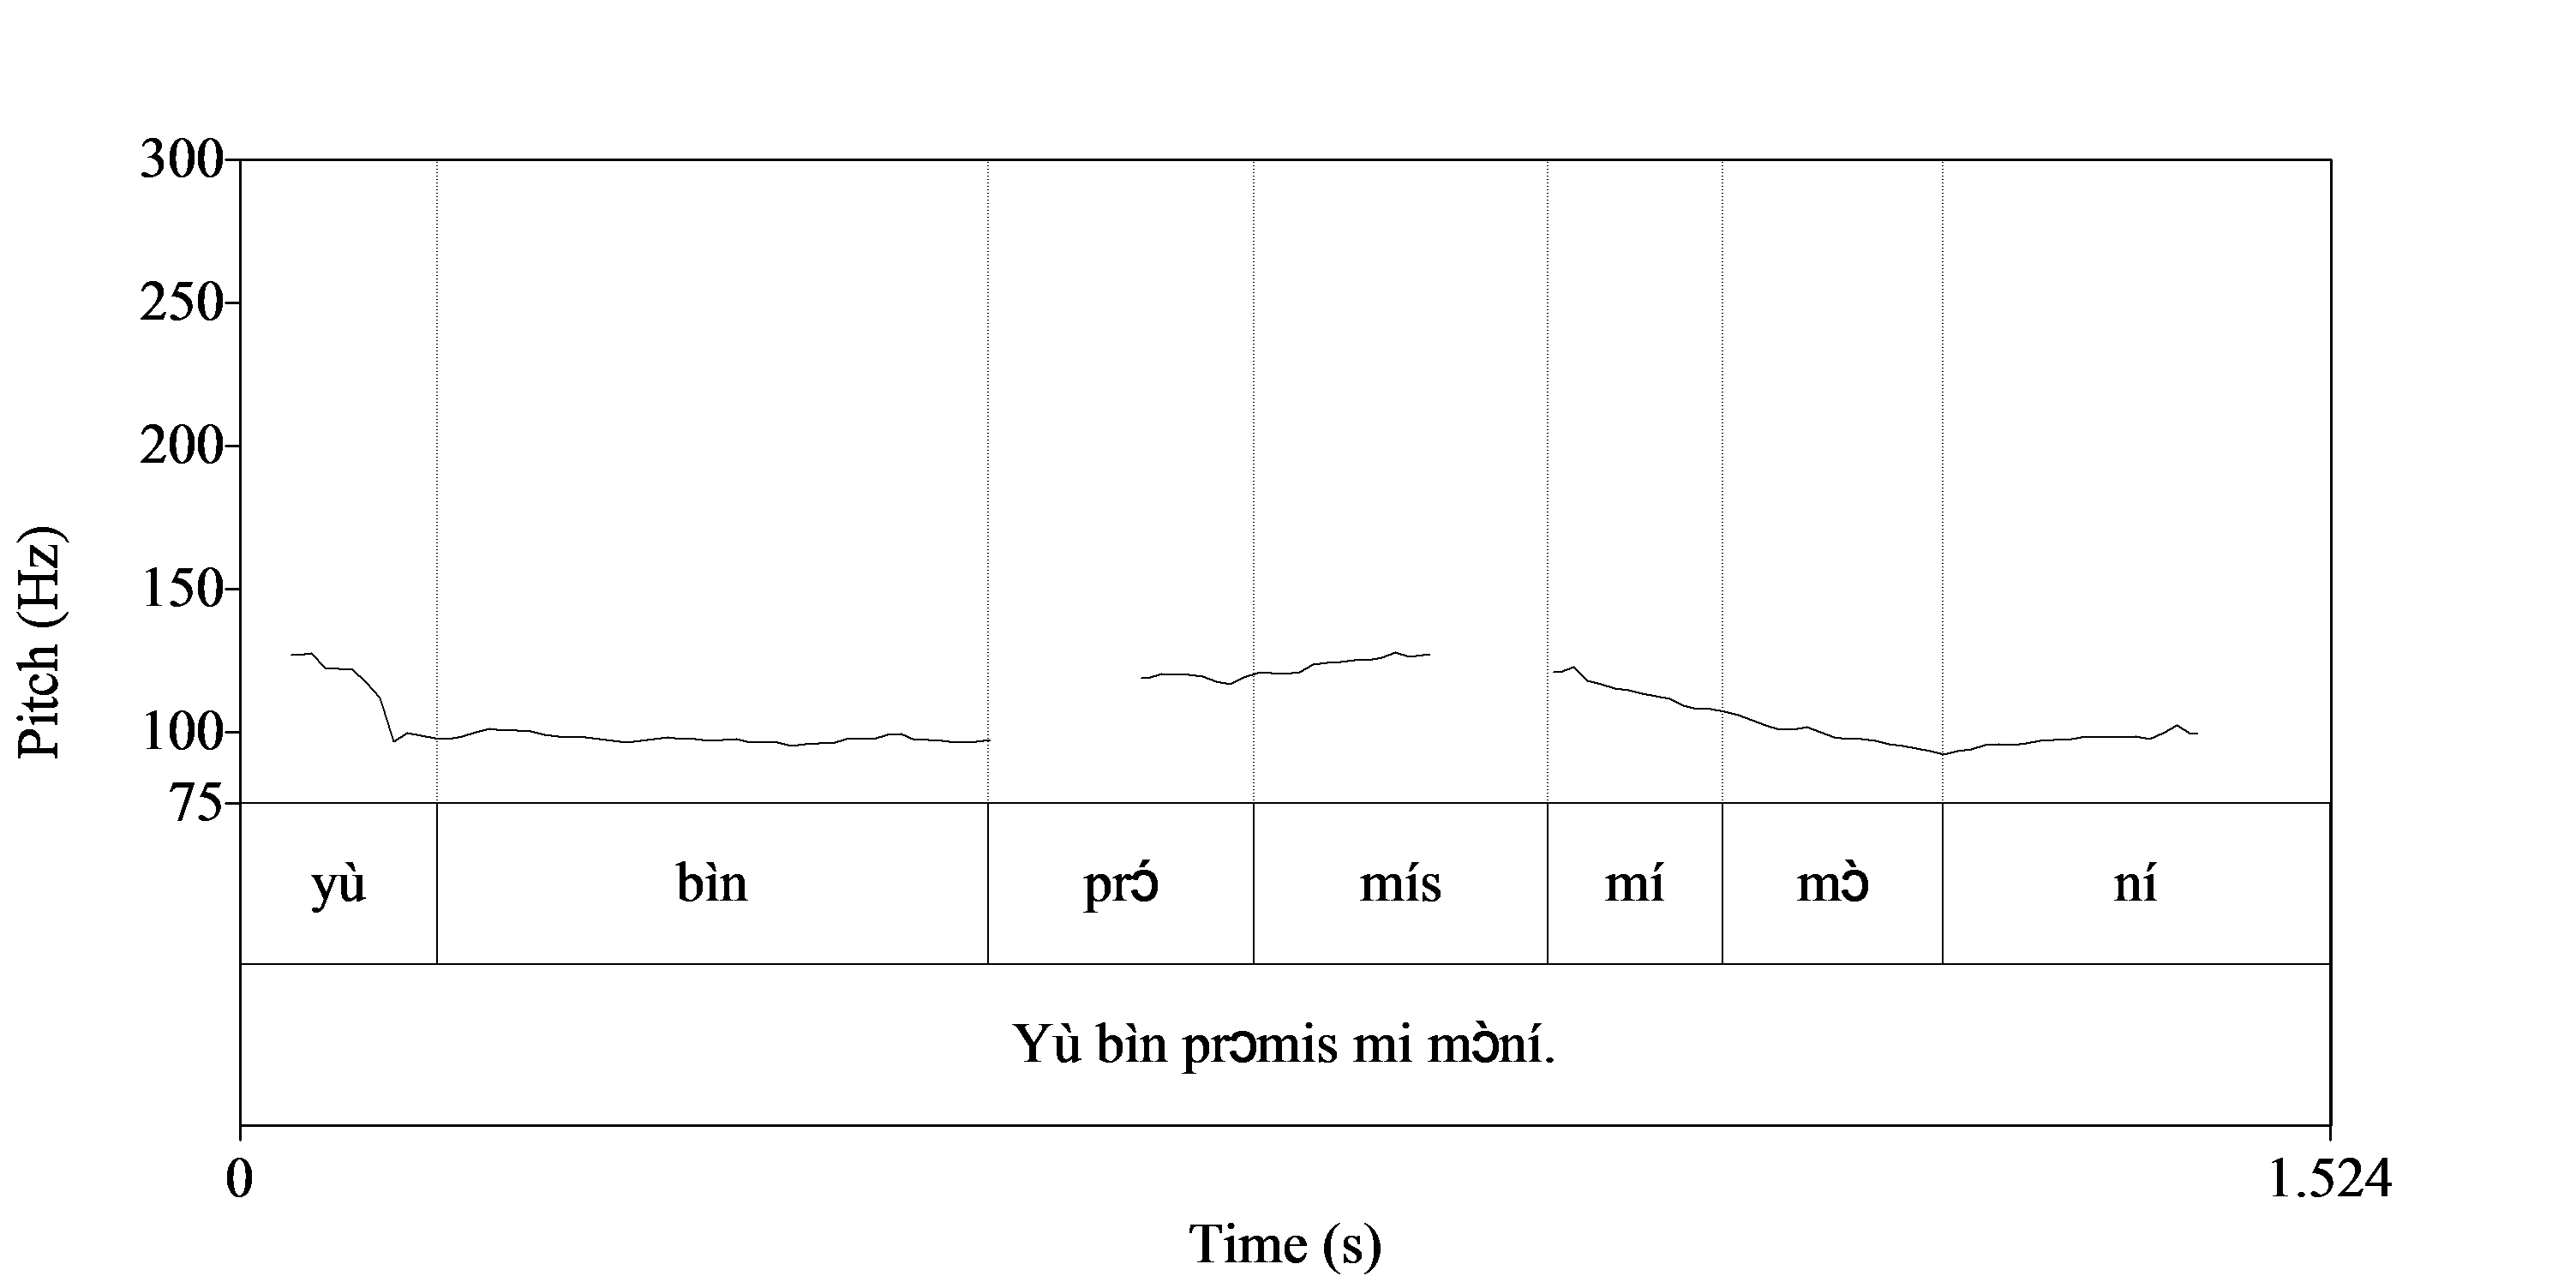
\includegraphics[height=.3\textheight]{figures/yakpomod-img13.png}
\label{fig:key:3.11}
\end{figure}
 


\ea%50
    \label{ex:key:50}
    \glll   Yu  bin  prɔ́mis  mí    mɔní.  →    Yu  bin  \textbf{prɔ́mis}  mí  mɔní.\\
\textsc{l}  \textsc{l}  \textsc{h.l}    \textsc{h}    \textsc{l.h}         {} \textsc{l}  \textsc{l}  \textbf{\textsc{h.h}}    \textsc{h}  \textsc{l.h}\\
\textsc{2sg}  \textsc{pst}  promise  \textsc{1sg.indp}  money\\
\glt ‘You promised me money.’
\z

An environment that is particularly conducive to rightward tone spreading is when the L-toned syllable of a bisyllabic word with an H.L. pattern is hemmed in by the preceding H tone and the H tone of a following object. In \figref{fig:key:3.12}, the L-toned syllable of \textit{fínis} ‘finish’ is raised in pitch approximately to the level of the following object \textit{skúl} ‘school’. The pitch trace in \figref{fig:key:3.13} exemplifies the same process with \textit{vɔ́mit} ‘vomit’ and the following object \textit{chɔ́p} ‘food’:

% TODO: put in a cuadrant

\begin{figure}
\caption{H tone spreading}
\label{fig:key:3.12}
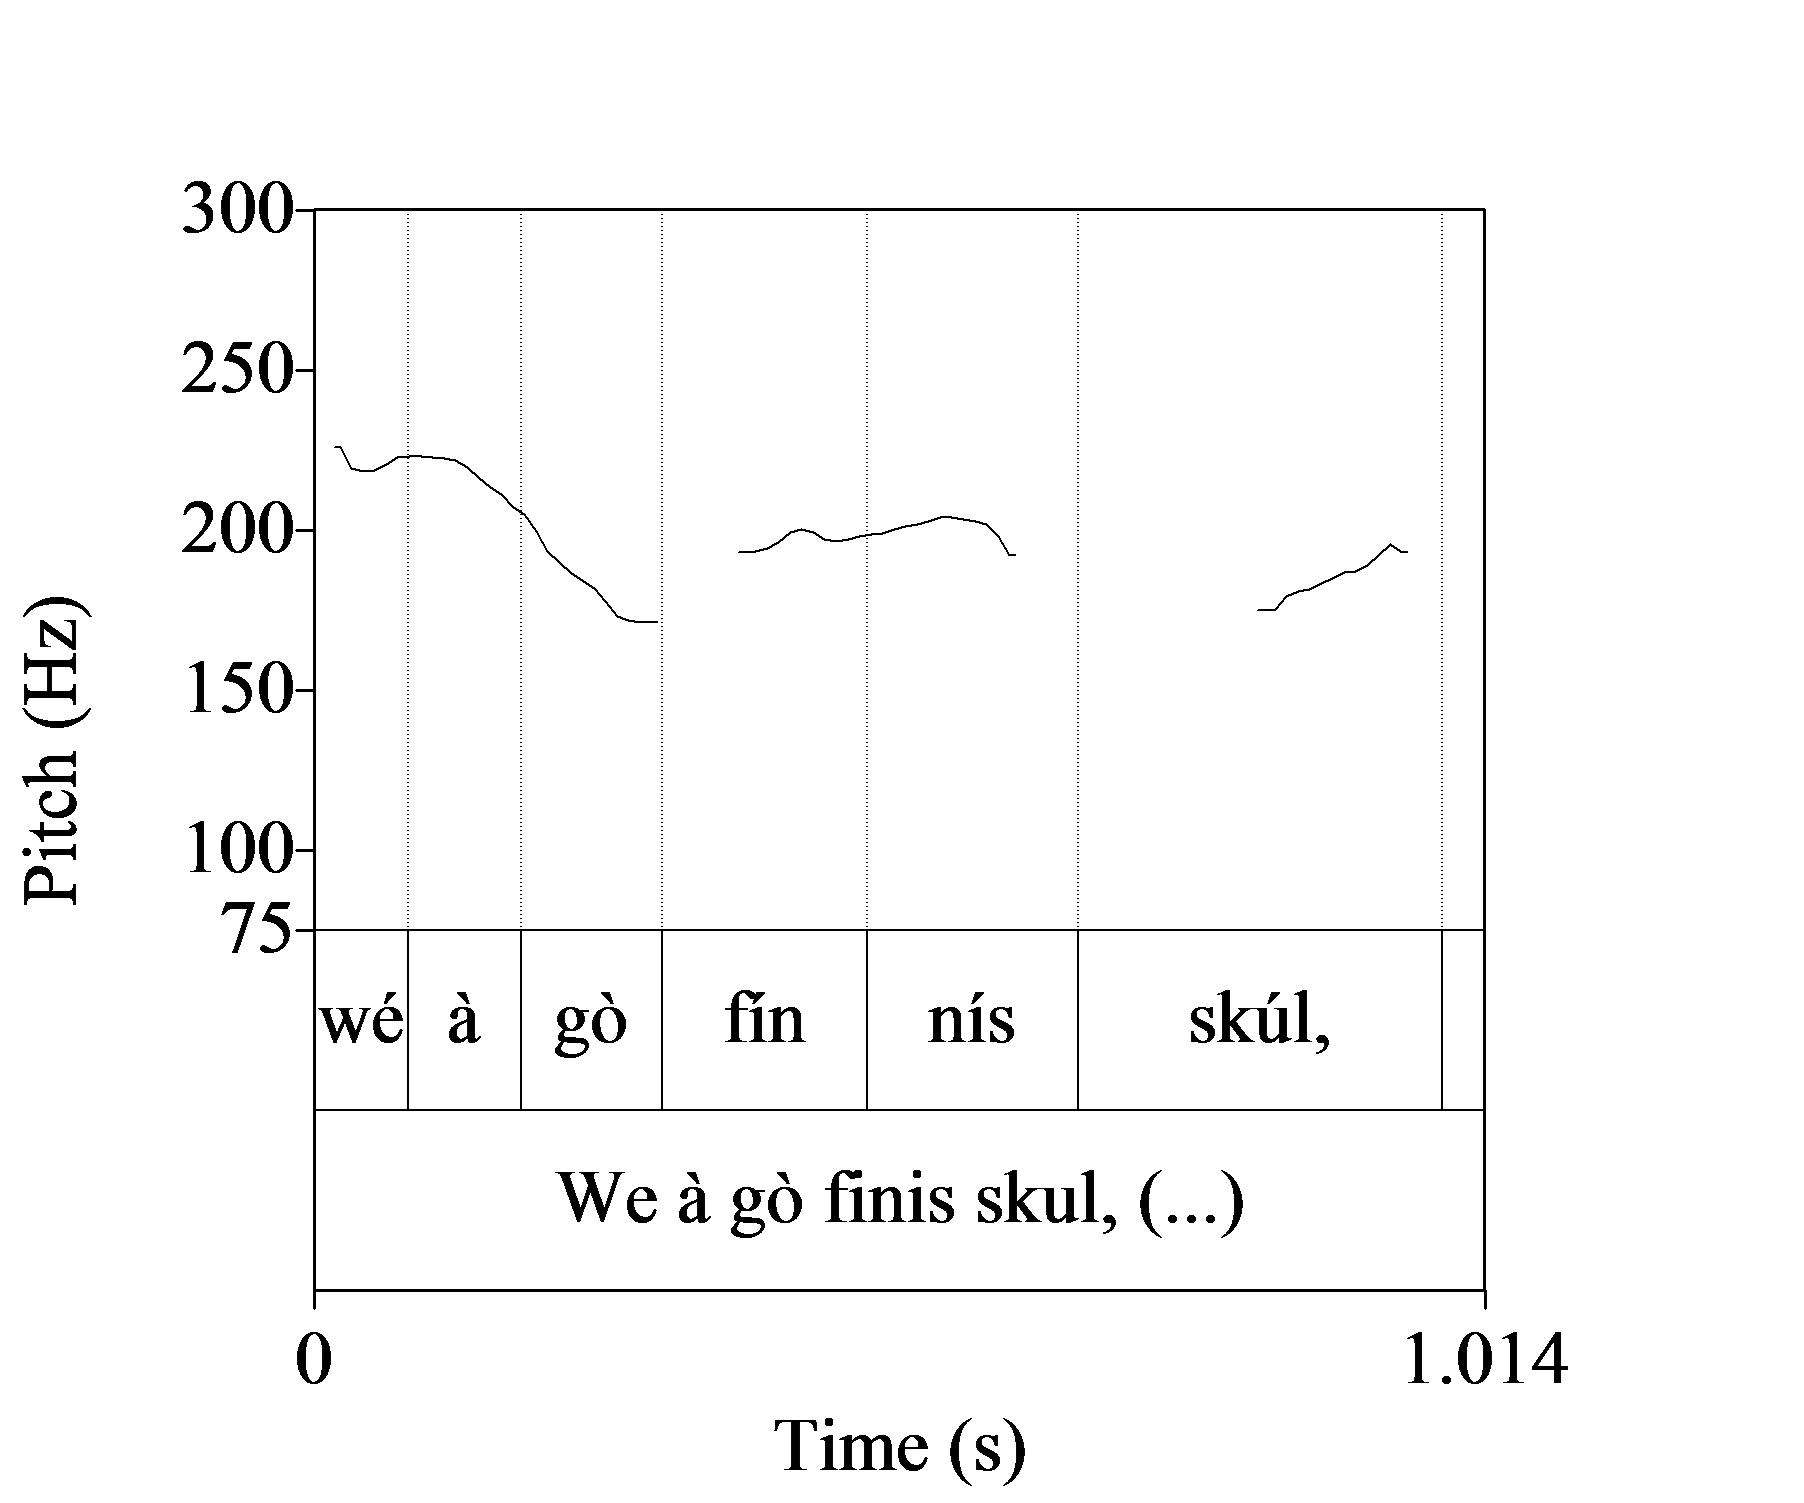
\includegraphics[height=.3\textheight]{figures/yakpomod-img14.png}
\end{figure}

\begin{figure}
\caption{H tone spreading}
\label{fig:key:3.13}
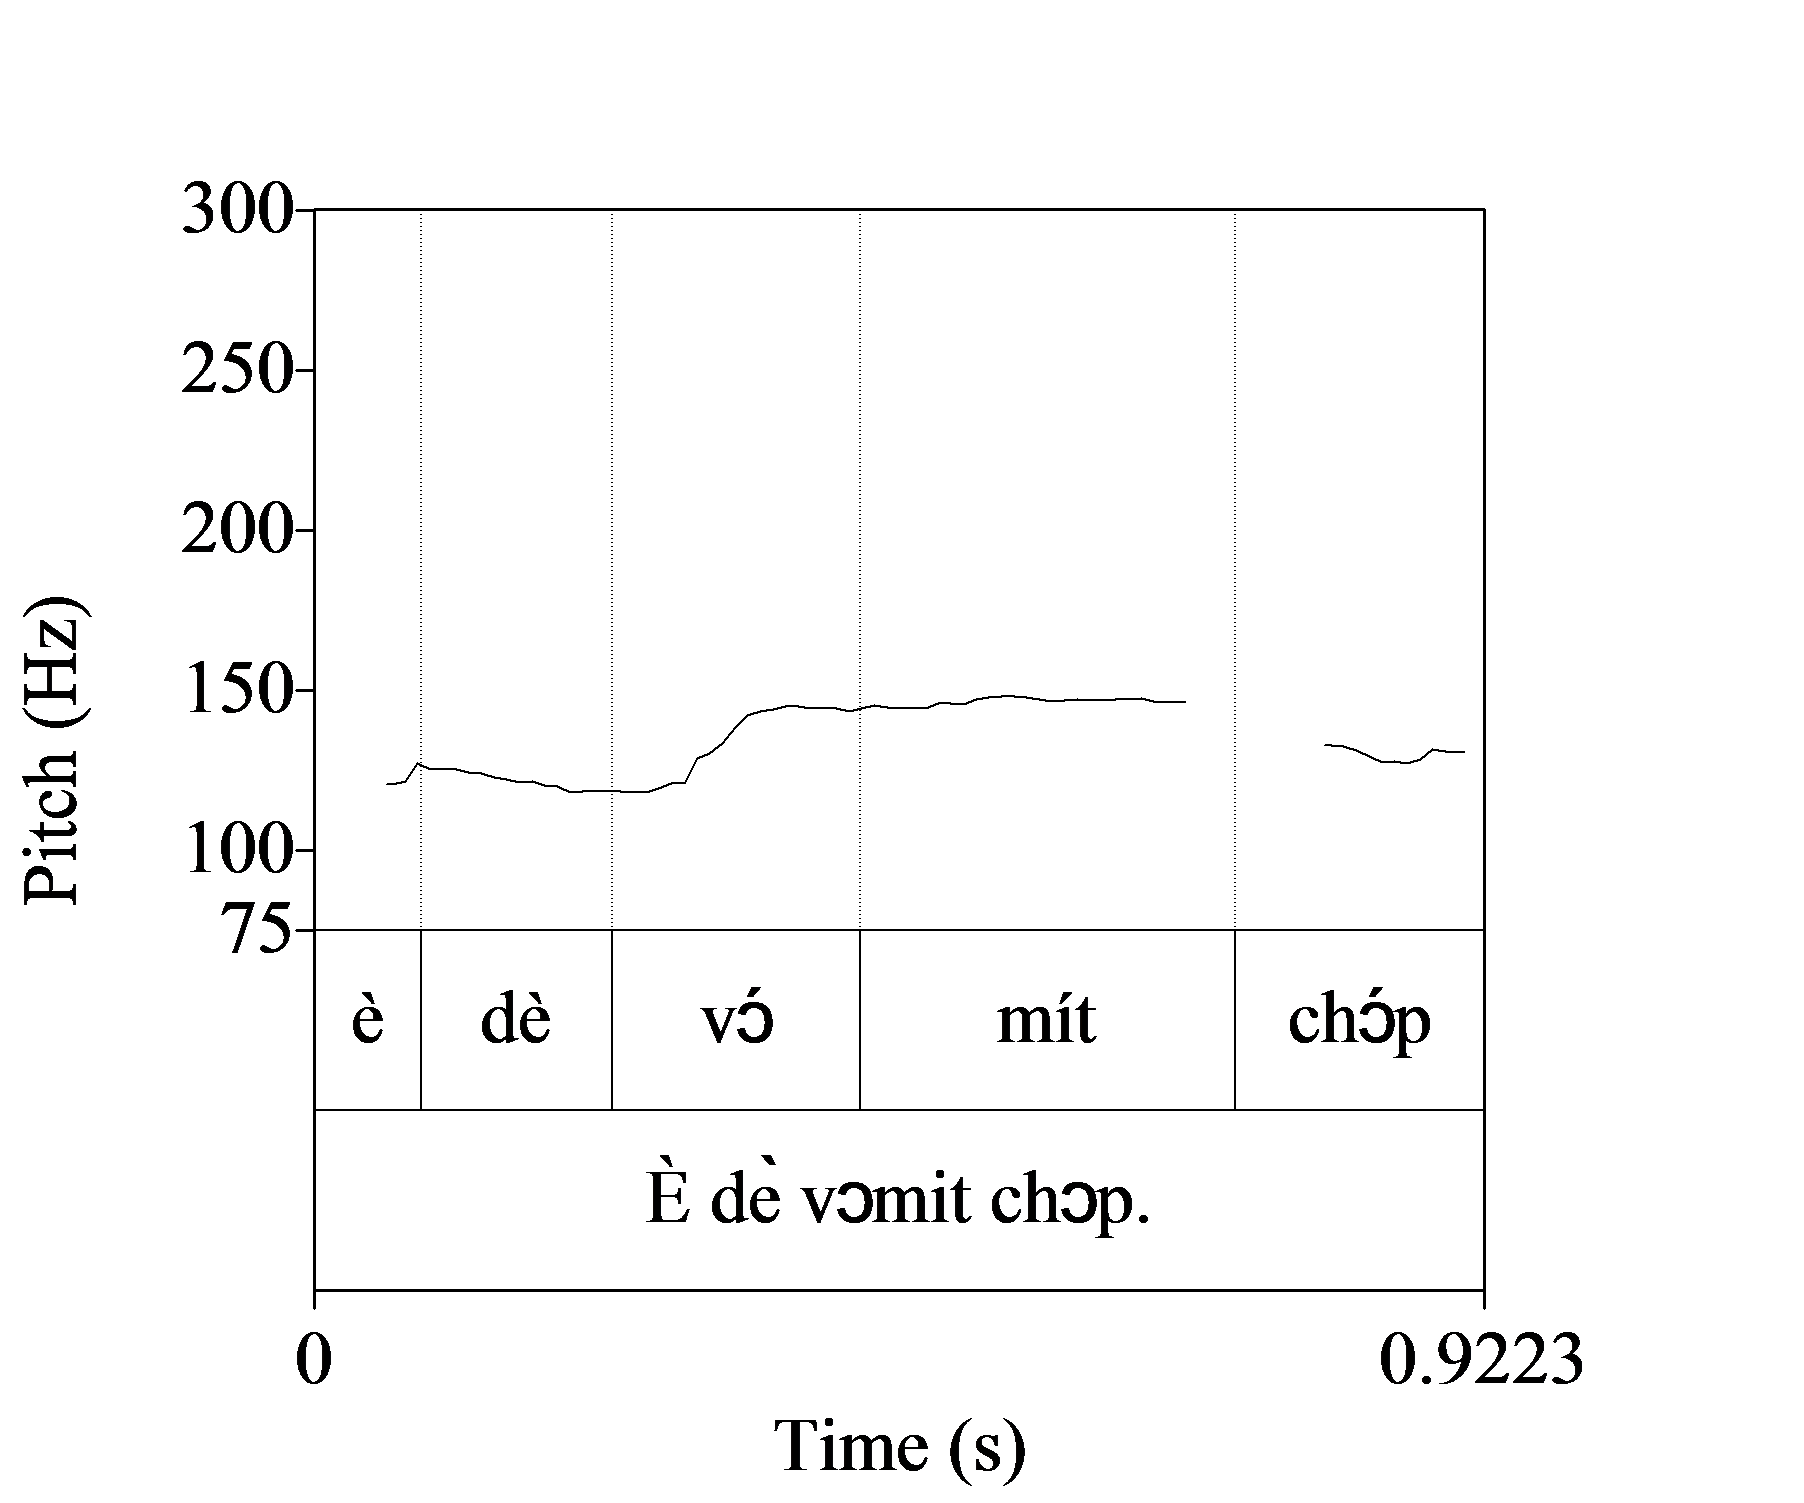
\includegraphics[height=.3\textheight]{figures/yakpomod-img15.png} 
\end{figure}

\ea\label{ex:key:51}
\glll Wé  a    go  fínis    skúl  (...)\\
\textsc{h}  \textsc{l}    \textsc{l}  \textsc{h.l}    \textsc{h}\\
\textsc{sub}  \textsc{1sg.sbj}  \textsc{pot}  finish  school\\
\glt  ‘When I finish school.’  →\\
\gll    Wé  a  go  \textstylePichiexamplebold{finís}  \textstylePichiexamplebold{skúl}  (...)\\
\textsc{h}  \textsc{l}  \textsc{l}  \textbf{\textsc{h.h}}    \textbf{\textsc{h}}\\
\z
\ea\label{ex:key:52}   
\glll E    de    vɔ́mit  chɔ́p.\\
\textsc{l}    \textsc{l}    \textsc{h.l}    \textsc{h}\\
\textsc{3sg.sbj}  \textsc{ipfv}    vomit  food\\
\glt  ‘He is vomiting (the) food.’  →\\
\gll E  de  \textstylePichiexamplebold{vɔmít}  \textstylePichiexamplebold{chɔ́p}.\\
\textsc{l}  \textsc{l}  \textbf{\textsc{h.h}  }  \textbf{\textsc{h}}\is{assimilation of segments“ r}\\
\z
A second phono-syntactic environment that favours rightward H tone spreading is a modifier-noun phrase. The L-toned syllable of a bisyllabic property item in prenominal position and with an H.L pattern may be raised to H if it is immediately followed by a noun with an initial (or only) H tone. An example for this process is provided in \REF{ex:key:58} further below. In the NP, the L-toned syllable of the modifier \textit{fúlis} ‘foolish’ is raised to an H tone because it is followed by the H-toned noun \textit{mán} ‘man’.

\subsection{Floating}\label{sec:3.2.2}

Pichi makes extensive use of floating boundary tones for the purpose of intonation. Aside from that, a lexical tone may be set afloat when two adjoining vowels merge or one of two adjoining vowels is deleted. Tone floating is particularly likely to occur in the contact zone between an H-toned high-frequency function word and a following L-toned vowel. In \figref{fig:key:3.14}, the final consonant /k/ of \textit{mék} ‘\textsc{sbjv}’ is deleted\index{}. This creates a vowel hiatus, which in turn leads to the deletion of the first, higher /e/ of \textit{mék} in favour of the second, lower vowel /à/. The rising–falling contour over \textit{mâ (mék=à)} is clearly visible. 


In \figref{fig:key:3.15}, the final segment of \textit{háw} ‘how’ is deleted and the lexical H tone is set afloat. The vowel merger between /a/ and the following low-toned dependent personal pronoun \textit{e} creates an HL contour tone: 

% TODO: put in quadrant

\begin{figure}
\caption{Vowel deletion sets tone afloat}
\label{fig:key:3.14}
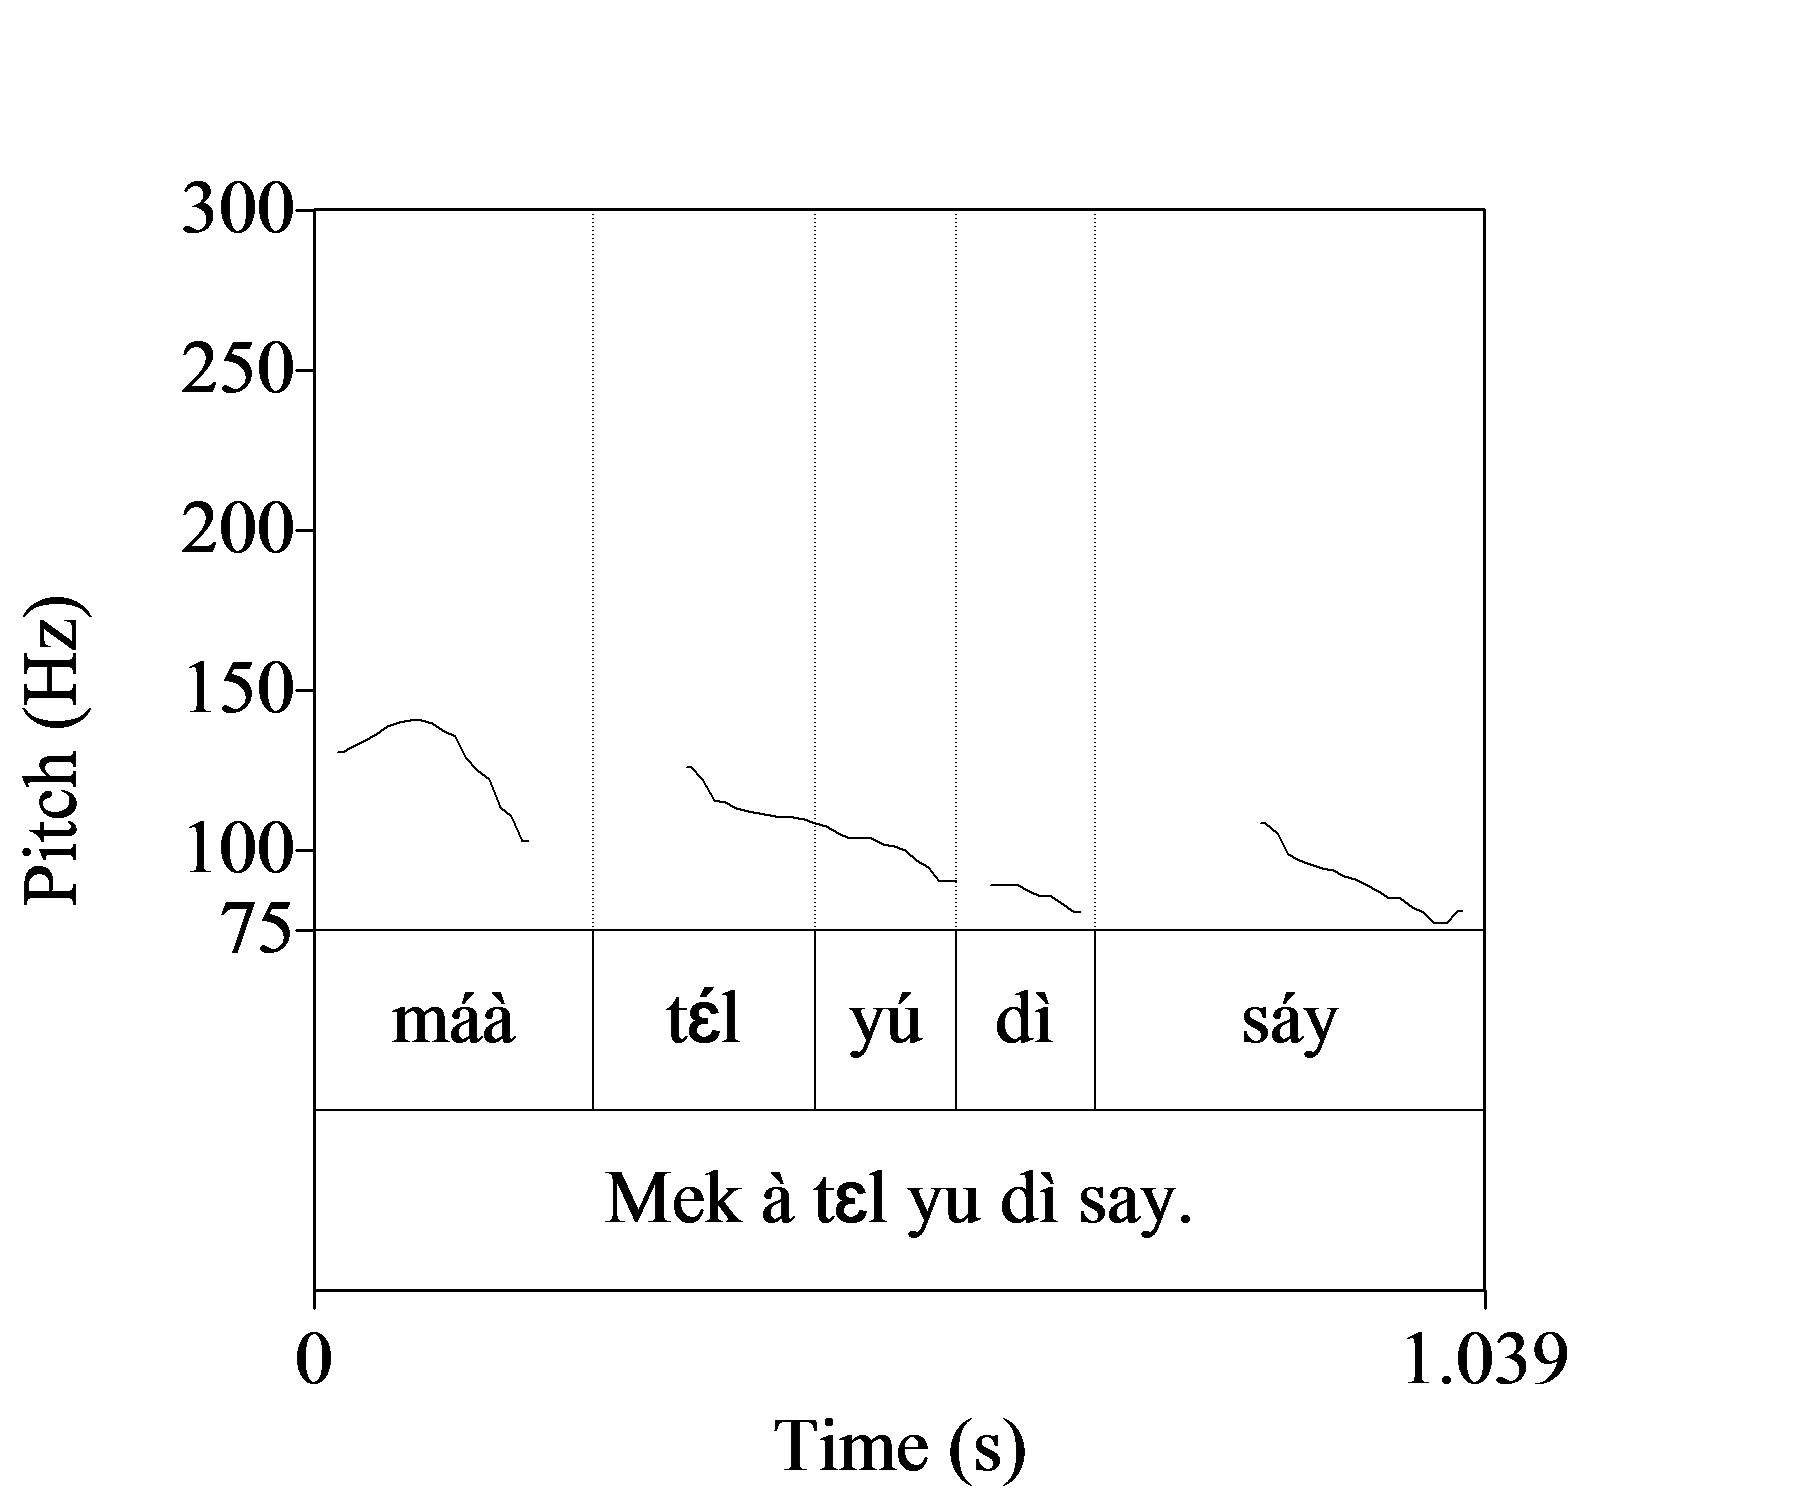
\includegraphics[height=.3\textheight]{figures/yakpomod-img16.png}
\end{figure}

\begin{figure}    
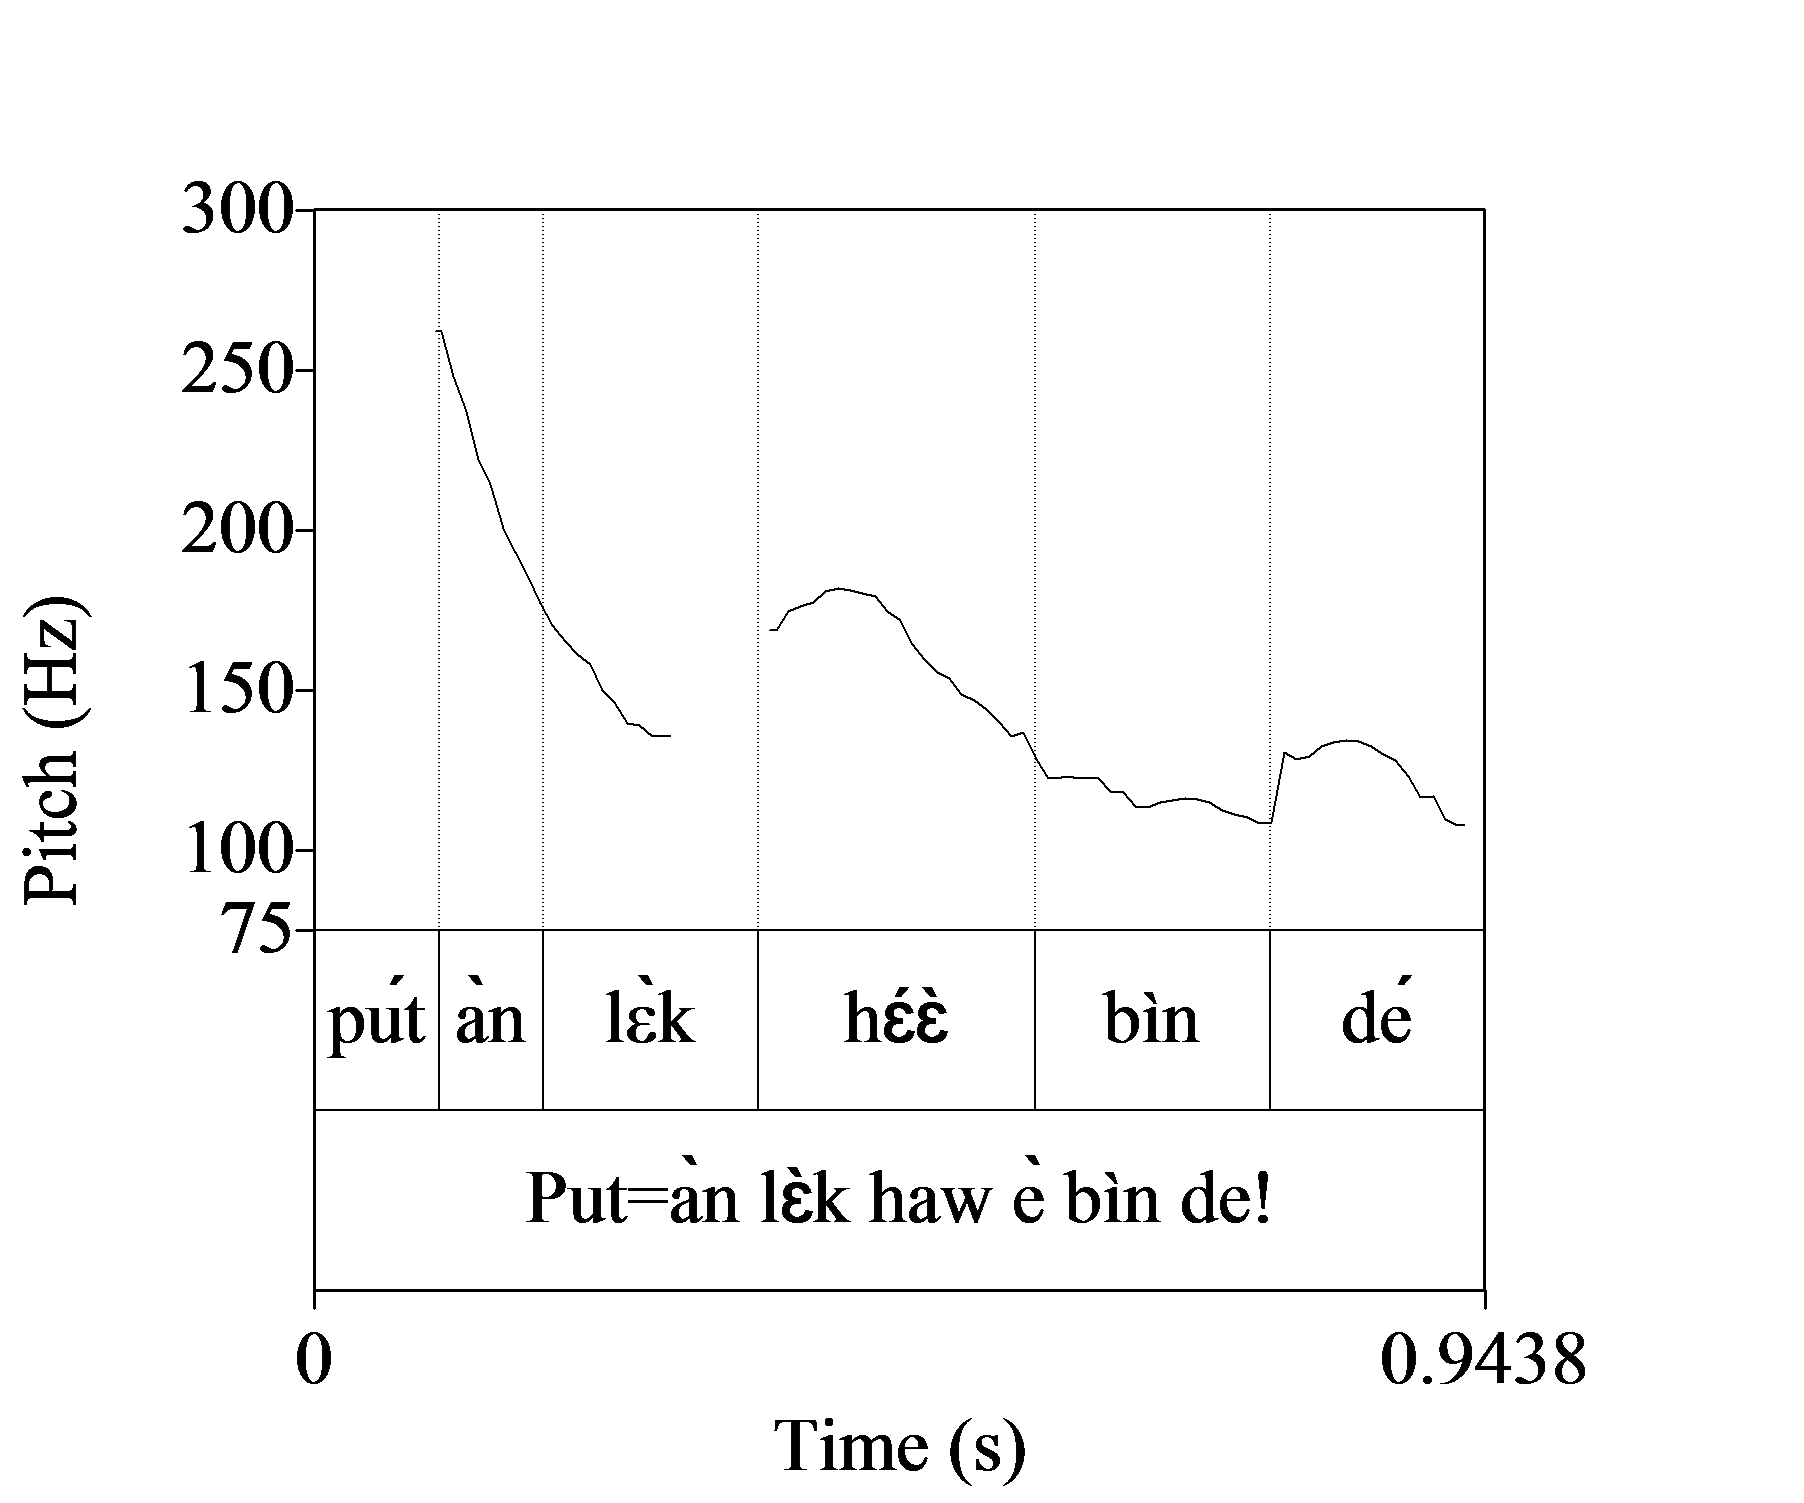
\includegraphics[height=.3\textheight]{figures/yakpomod-img17.png}
\caption{Vowel merger sets tone afloat}
\label{fig:key:3.15} 
\end{figure}

\ea\label{ex:key:53}
\glll Mék    a    tɛ́l  yú    di  sáy.\\
\textsc{h}    \textsc{l}    \textsc{h}  \textsc{h}    \textsc{l}  \textsc{h}\\
\textsc{sbjv}    \textsc{1sg.sbj}  tell  \textsc{2sg.indp}  \textsc{def}  side\\
\glt ‘Let me tell you the place.’    →\\
\gll Mâ    tɛ́l  yú  di  sáy.\\
\textbf{\textsc{hl}}    \textsc{h}  \textsc{h}  \textsc{l}  \textsc{h}\\
\z

\ea\label{ex:key:54}
\glll   Pút=an    lɛk  háw  e    bin  dé!\\
\textsc{h}  \textsc{l}    \textsc{l}  \textsc{h}  \textsc{l}    \textsc{l}  \textsc{h}\\
put=\textsc{3sg.obj}  like  how  \textsc{3sg.sbj}  \textsc{pst}  \textsc{be.loc}\\
\glt ‘Put it like it was!’    →\\
\gll Pút=an  lɛk  \textbf{hɛ}  bin  dé!\\
\textsc{h}  \textsc{l}  \textsc{l}  \textbf{\textsc{hl}}  \textsc{l}  \textsc{h}\\
\z
\subsection{Downdrift and downstep}\label{sec:3.2.3}

Downdrift and downstep contribute to a general downward cline of pitch in utterances. An utterance normally begins with a high pitch onset and declines progressively with every lexical tone. Downdrift (indicated by ↓H) causes an H to be lowered by a preceding L tone as in \figref{fig:key:3.16}. The overall effect of downdrift is visible by the roughly equivalent pitch over the initial L-toned personal pronoun \textit{a} ‘\textsc{1sg.sbj}’ and the final H-toned noun \textit{hós} ‘house’:

\begin{figure}
\caption{Downdrift}
\label{fig:key:3.16}
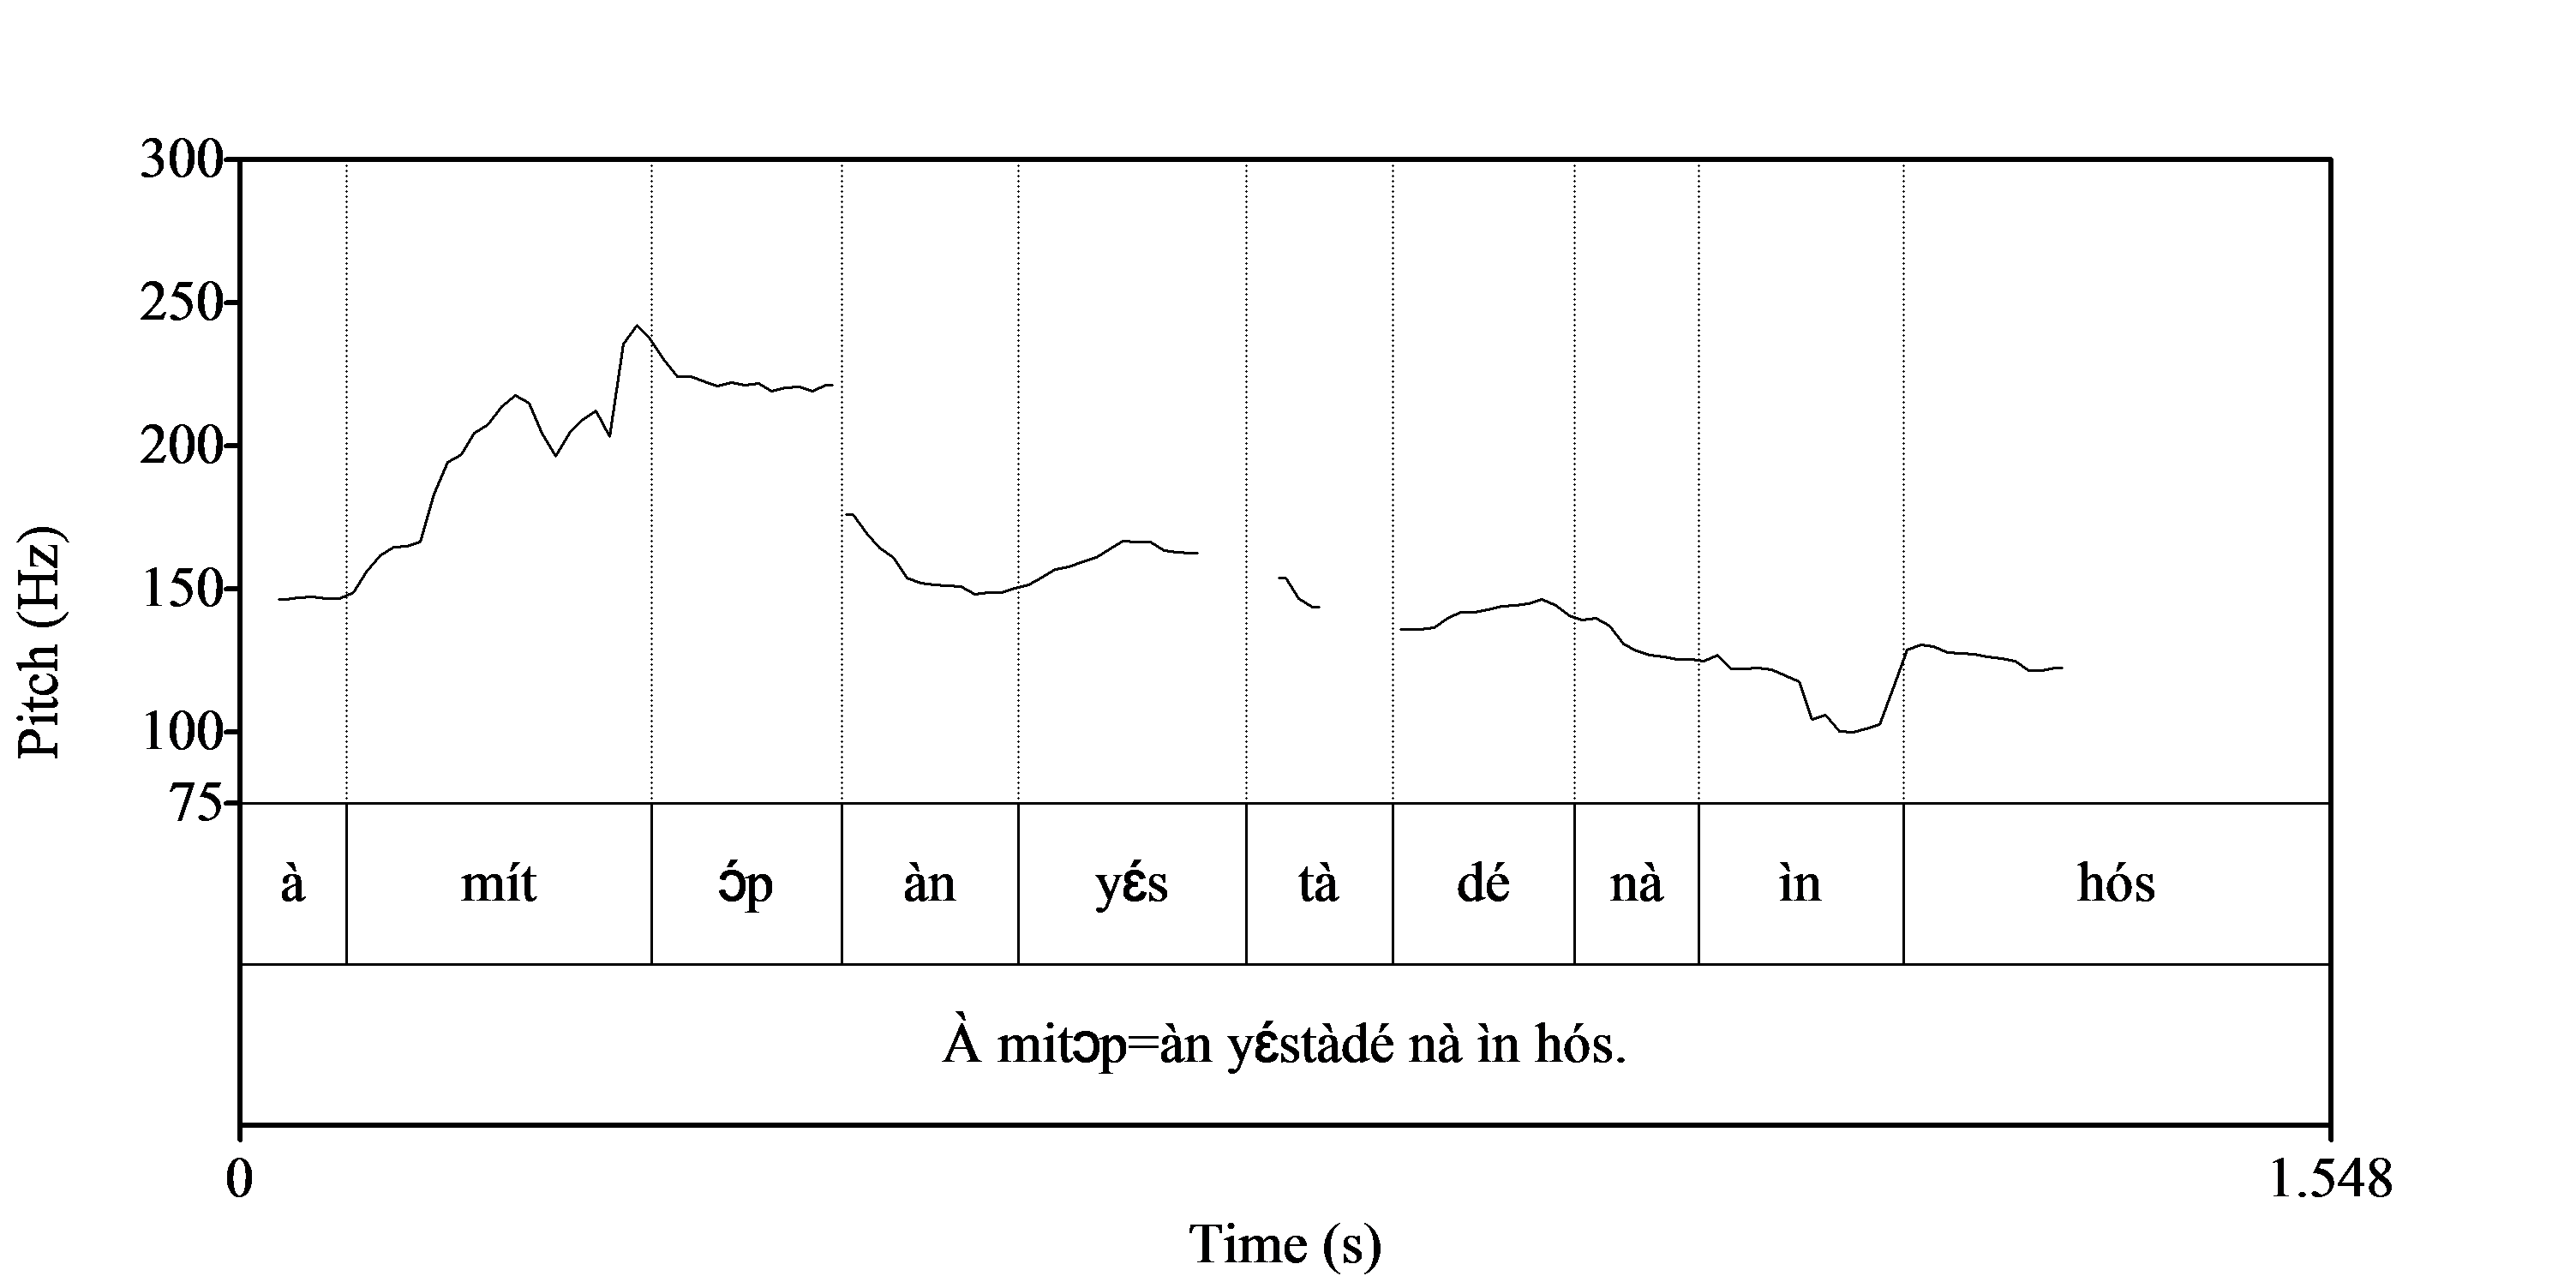
\includegraphics[height=.3\textheight]{figures/yakpomod-img18.png}
\end{figure}
 


\ea%55
    \label{ex:key:55}
    \glll   A    mítɔp=an  yɛ́stadé    na  in  hós.\\
\textsc{l}    \textstylePichiexamplebold{\textmd{\textsc{h}}}\textsc{.h=l}    \textsc{↓}\textbf{\textsc{h}}\textsc{.l.↓}\textbf{\textsc{h}}    \textsc{l}  \textsc{l}  \textsc{↓}\textbf{\textsc{h}}\is{downdrift} \\
\textsc{1sg.sbj}  meet=\textsc{3sg}  yesterday  \textsc{loc}  \textsc{3sg.poss}  house\\
\glt ‘I met him yesterday in his house.’    
\z


The second phenomenon involving declination is downstep\is{downstep} (indicated by –H). In a series of adjacent H tones, each tone may be lowered successively in relation to the preceding one. Downstep is exemplified below by the two successive homophones in \figref{fig:key:3.17} and the iteration in \figref{fig:key:3.18} below. We also find downdrift in both examples:

% TODO: put in quadrant
 
\begin{figure}
\caption{Downstep}
\label{fig:key:3.17}
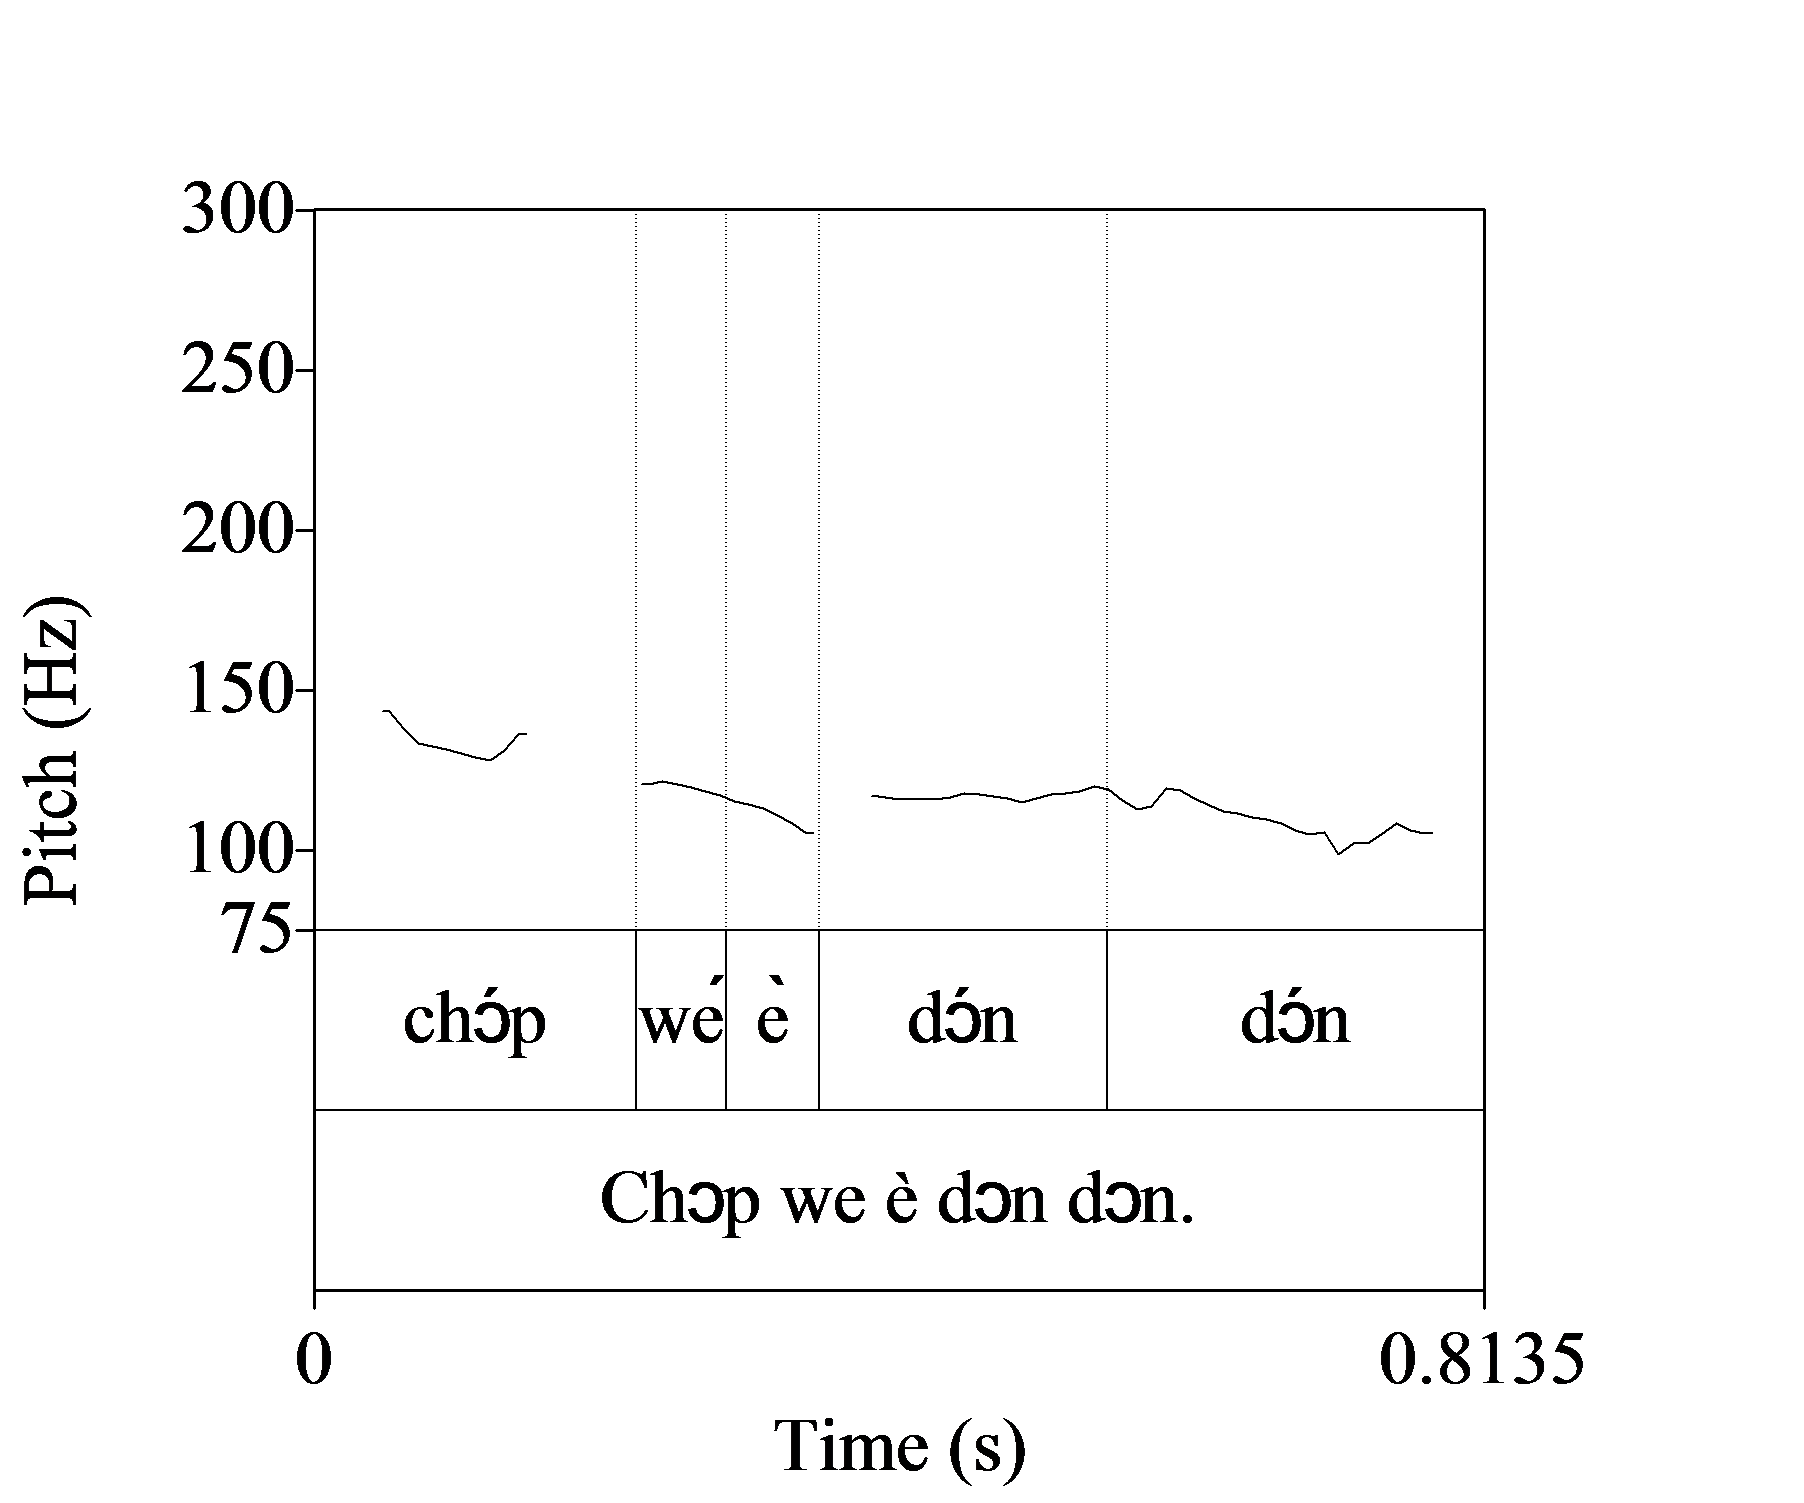
\includegraphics[height=.3\textheight]{figures/yakpomod-img19.png}
\end{figure}

\begin{figure}    
\caption{Downstep}
\label{fig:key:3.18}
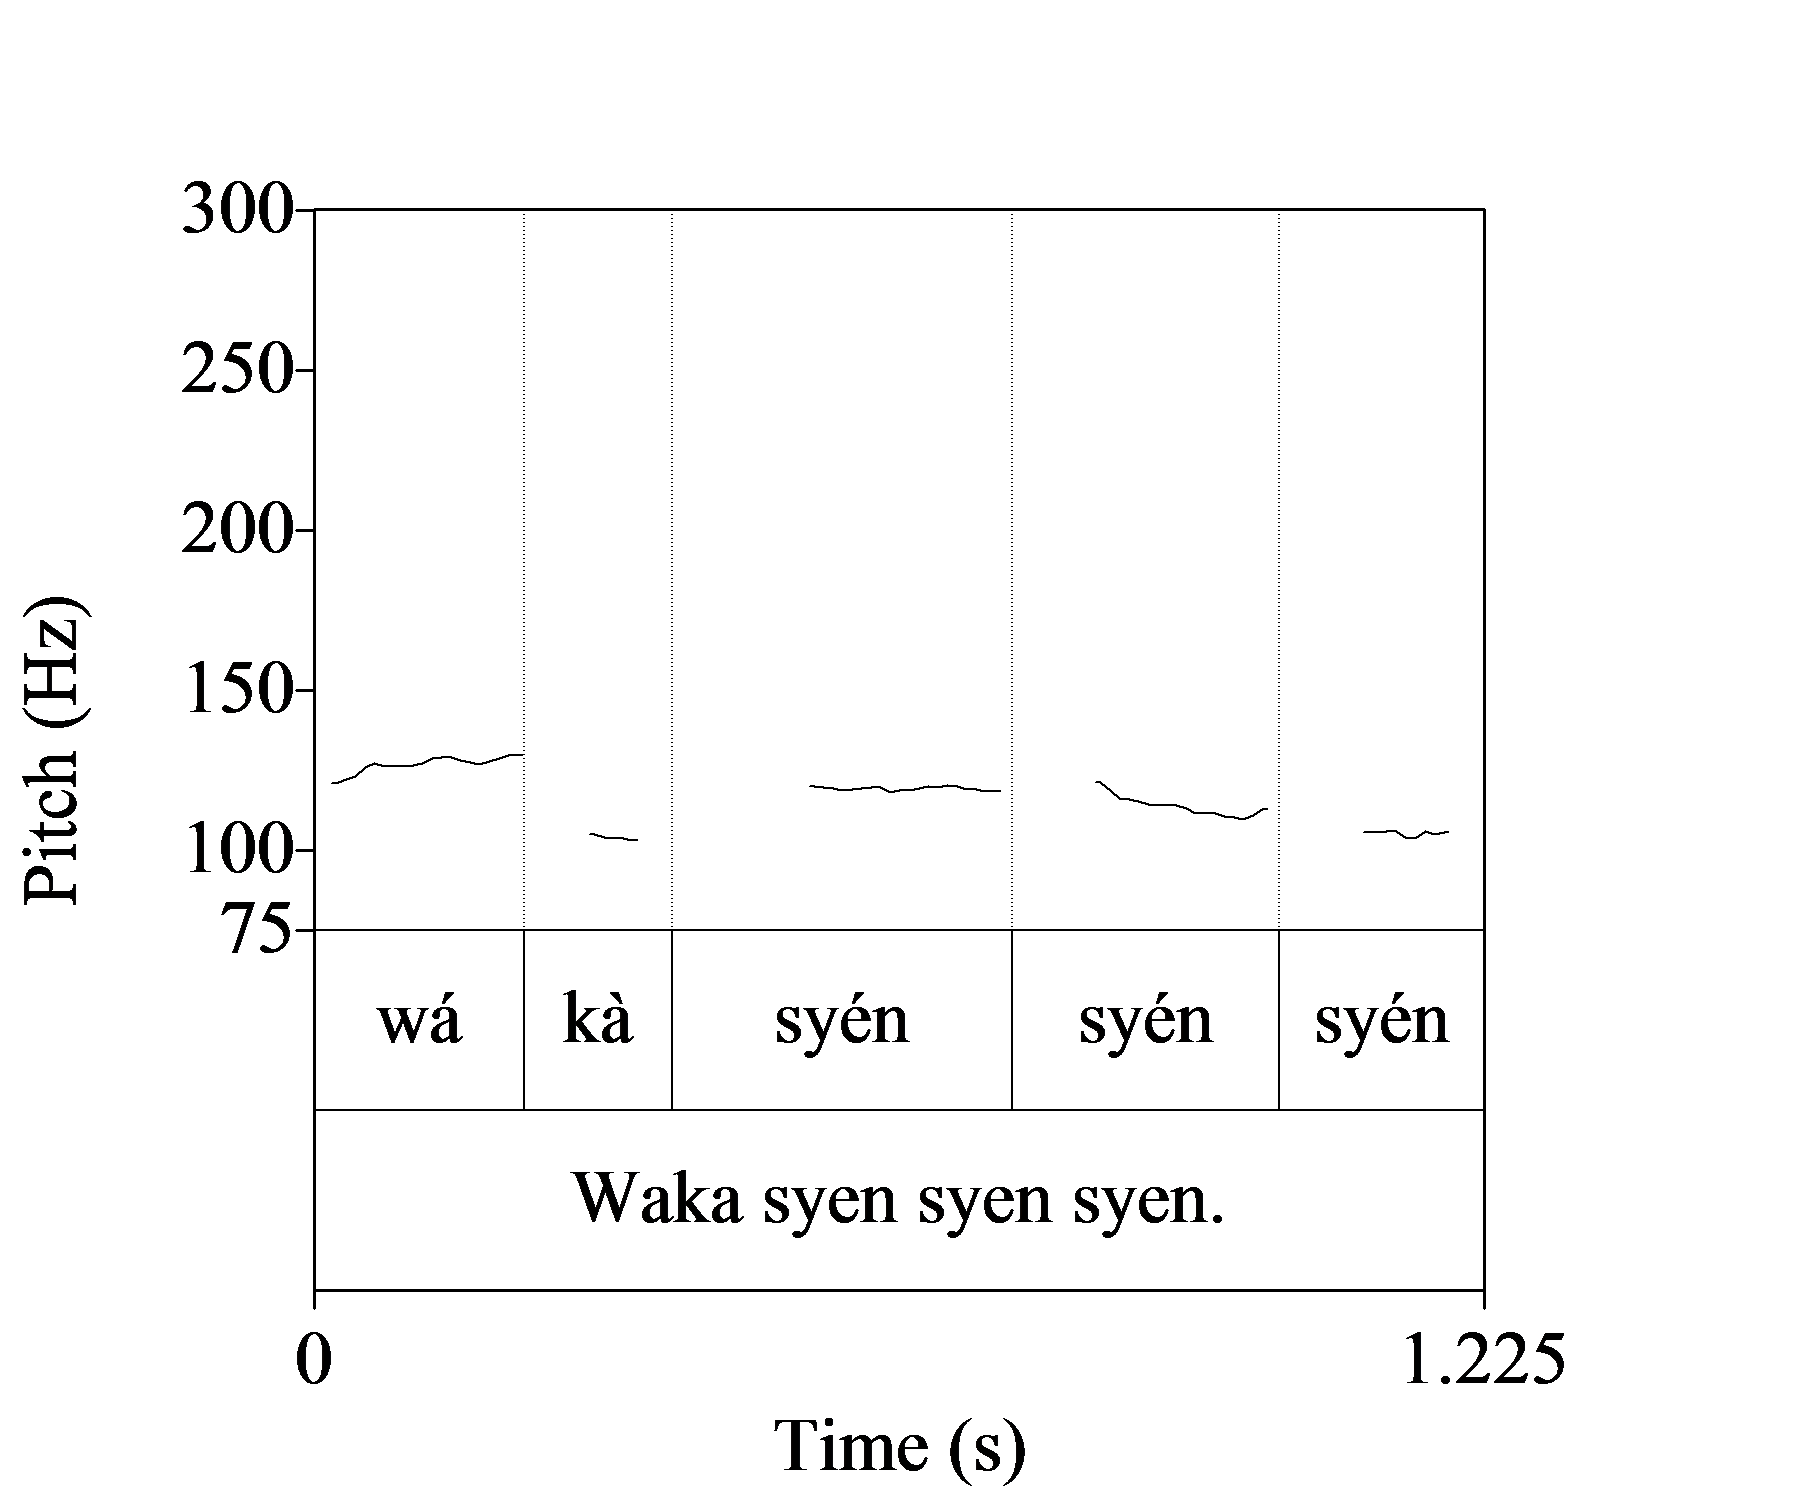
\includegraphics[height=.3\textheight]{figures/yakpomod-img20.png} 
\end{figure}

\ea\label{ex:key:56}
\glll Chɔ́p  wé  e    \textbf{dɔ́n}  \textbf{dɔ́n}.\\
\textsc{h}    \textbf{\textsc{{}-h}}  \textsc{l}    \textsc{↓}\textsc{h}  \textbf{\textsc{{}-h}} \\
food    \textsc{sub}  \textsc{3sg.sbj}  \textsc{prf}  done\\
\glt ‘Food that is done.’
\z

\ea\label{ex:key:57}
\glll   Wáka  sén    \textbf{sén}    \textbf{sén}.\\
\textsc{h.l}    \textsc{↓}\textsc{h}    \textbf{\textsc{{}-h}}    \textbf{\textsc{{}-h}}\\
walk  same  \textsc{rep}    \textsc{rep}\\
\glt ‘Walk exactly in one line.’
\z
\subsection{Deletion}\label{sec:3.2.4}

Tone deletion occurs in two contexts. In compounds (including reduplications), the lexical H tone over the first component is deleted (also see \citealt{Yakpo2012}). The syllable whose tone has been deleted becomes L-toned. The second component retains its original tone pattern. Tone deletion therefore forms an intrinsic part of a derivational process in Pichi (cf. \sectref{sec:4.3}). The second context in which tone deletion occurs is when a boundary tone overrides the utterance-final lexical tone of a word (cf. \sectref{sec:3.4.4} ).

\figref{fig:key:3.19} presents the pitch trace of an NP headed by the noun \textit{mán} ‘man’. The noun is modified prenominally by the verb \textit{fúlis} ‘(be) foolish’, which has an H.L tone pattern. The pitch of the utterance-final H tone over \textit{mán} stands at roughly the same level (albeit slightly downstepped and falling due to declarative intonation) as that of the preceding H tones over the first and second syllables of \textit{fúlis}. Note that the second, lexically L-toned syllable of \textit{fúlis} bears a phonetic H tone due to tonal plateauing (cf. \sectref{sec:3.2.1}):

\begin{figure}
\caption{Simplex noun}
\label{fig:key:3.19}
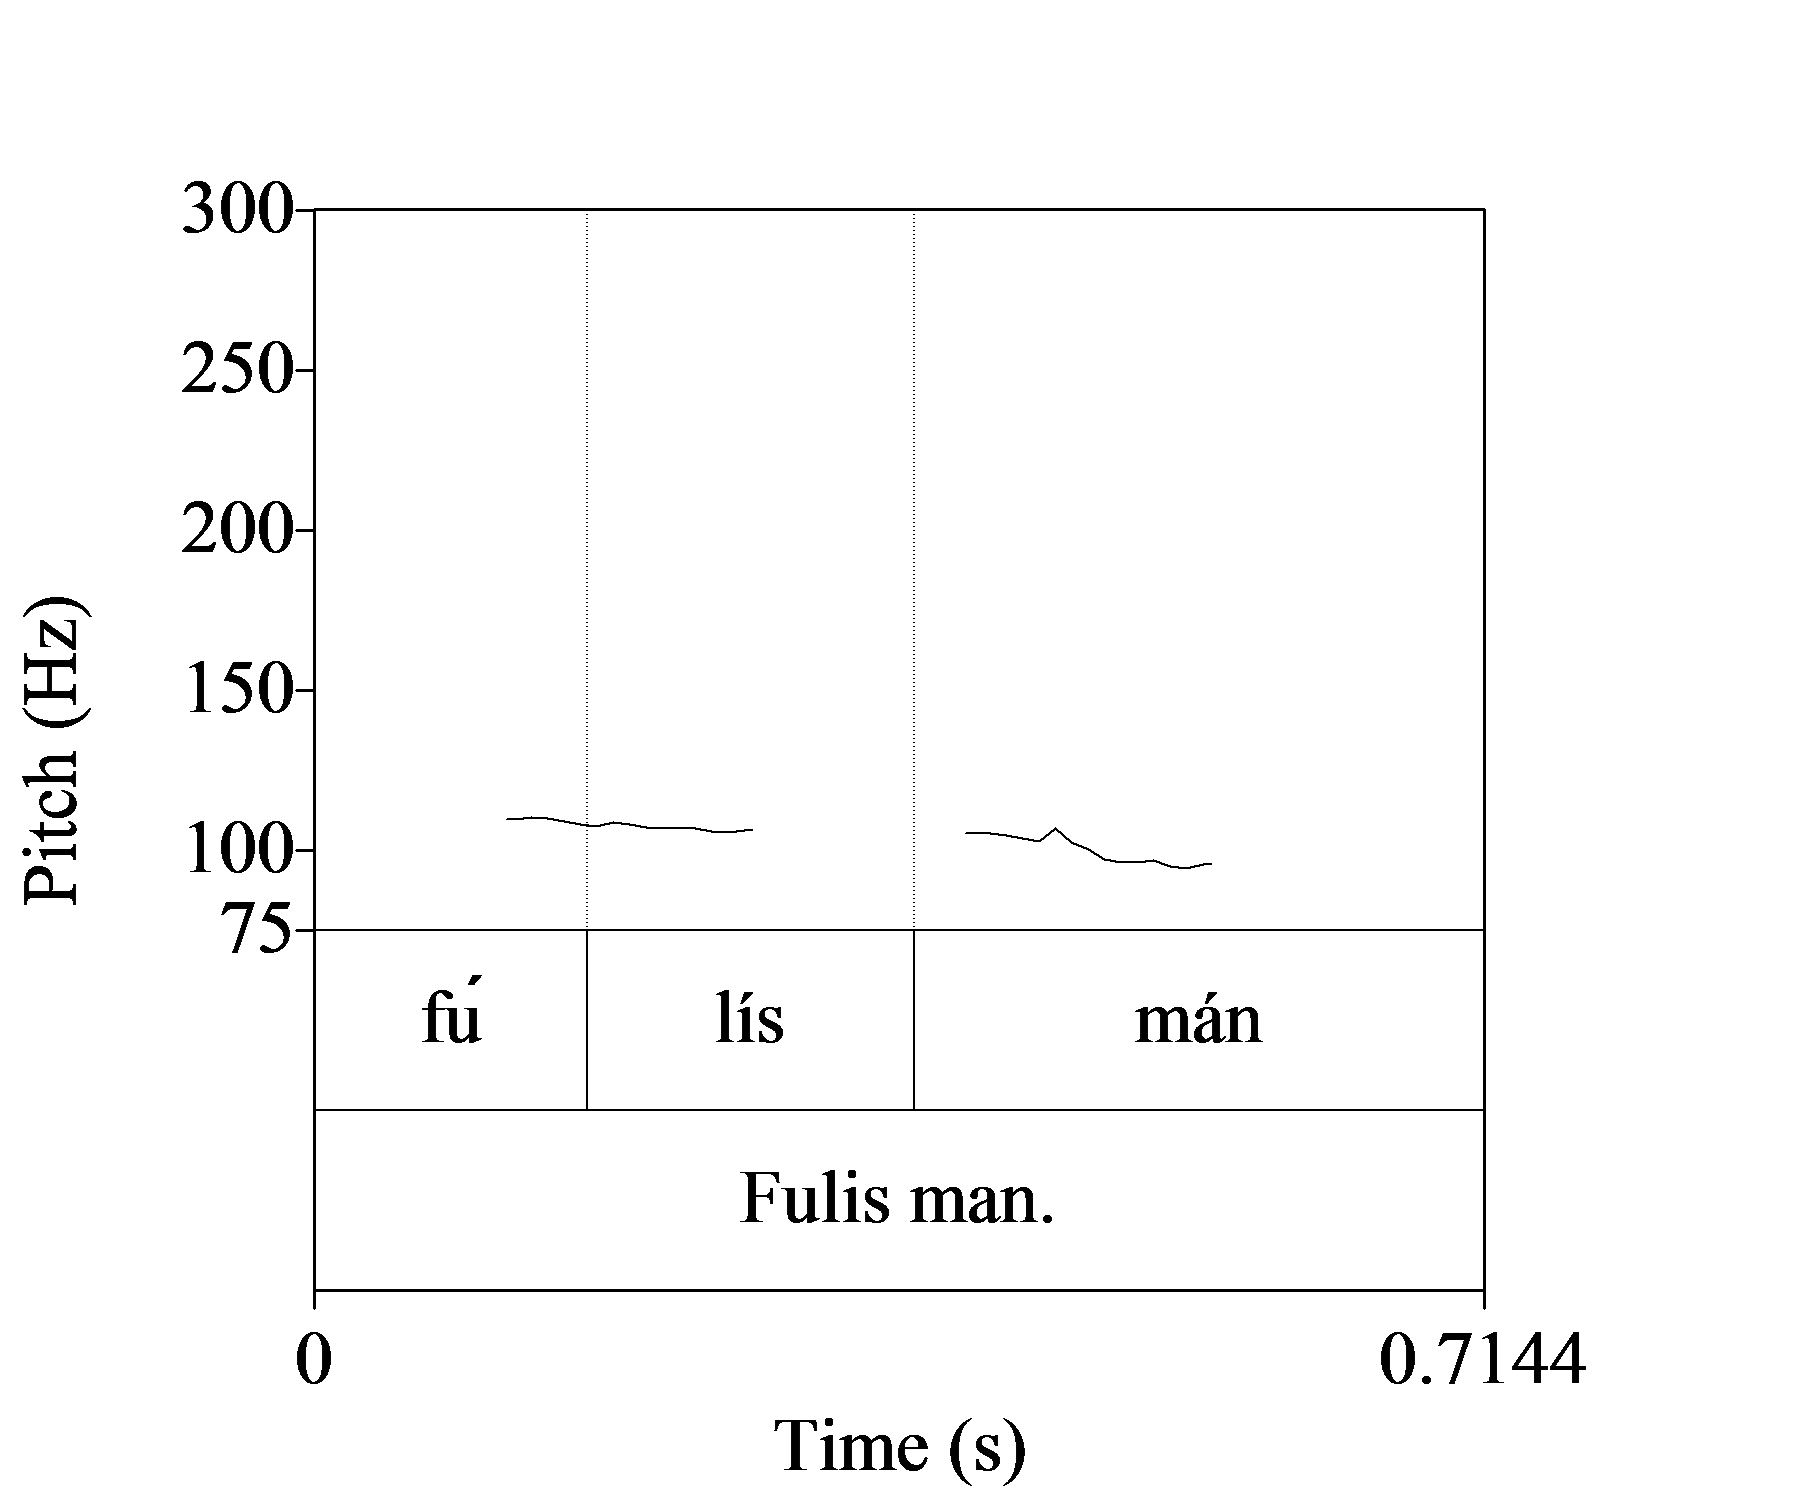
\includegraphics[height=.3\textheight]{figures/yakpomod-img21.png}
\end{figure}

\begin{figure}
\caption{Compound noun}
\label{fig:key:3.20}
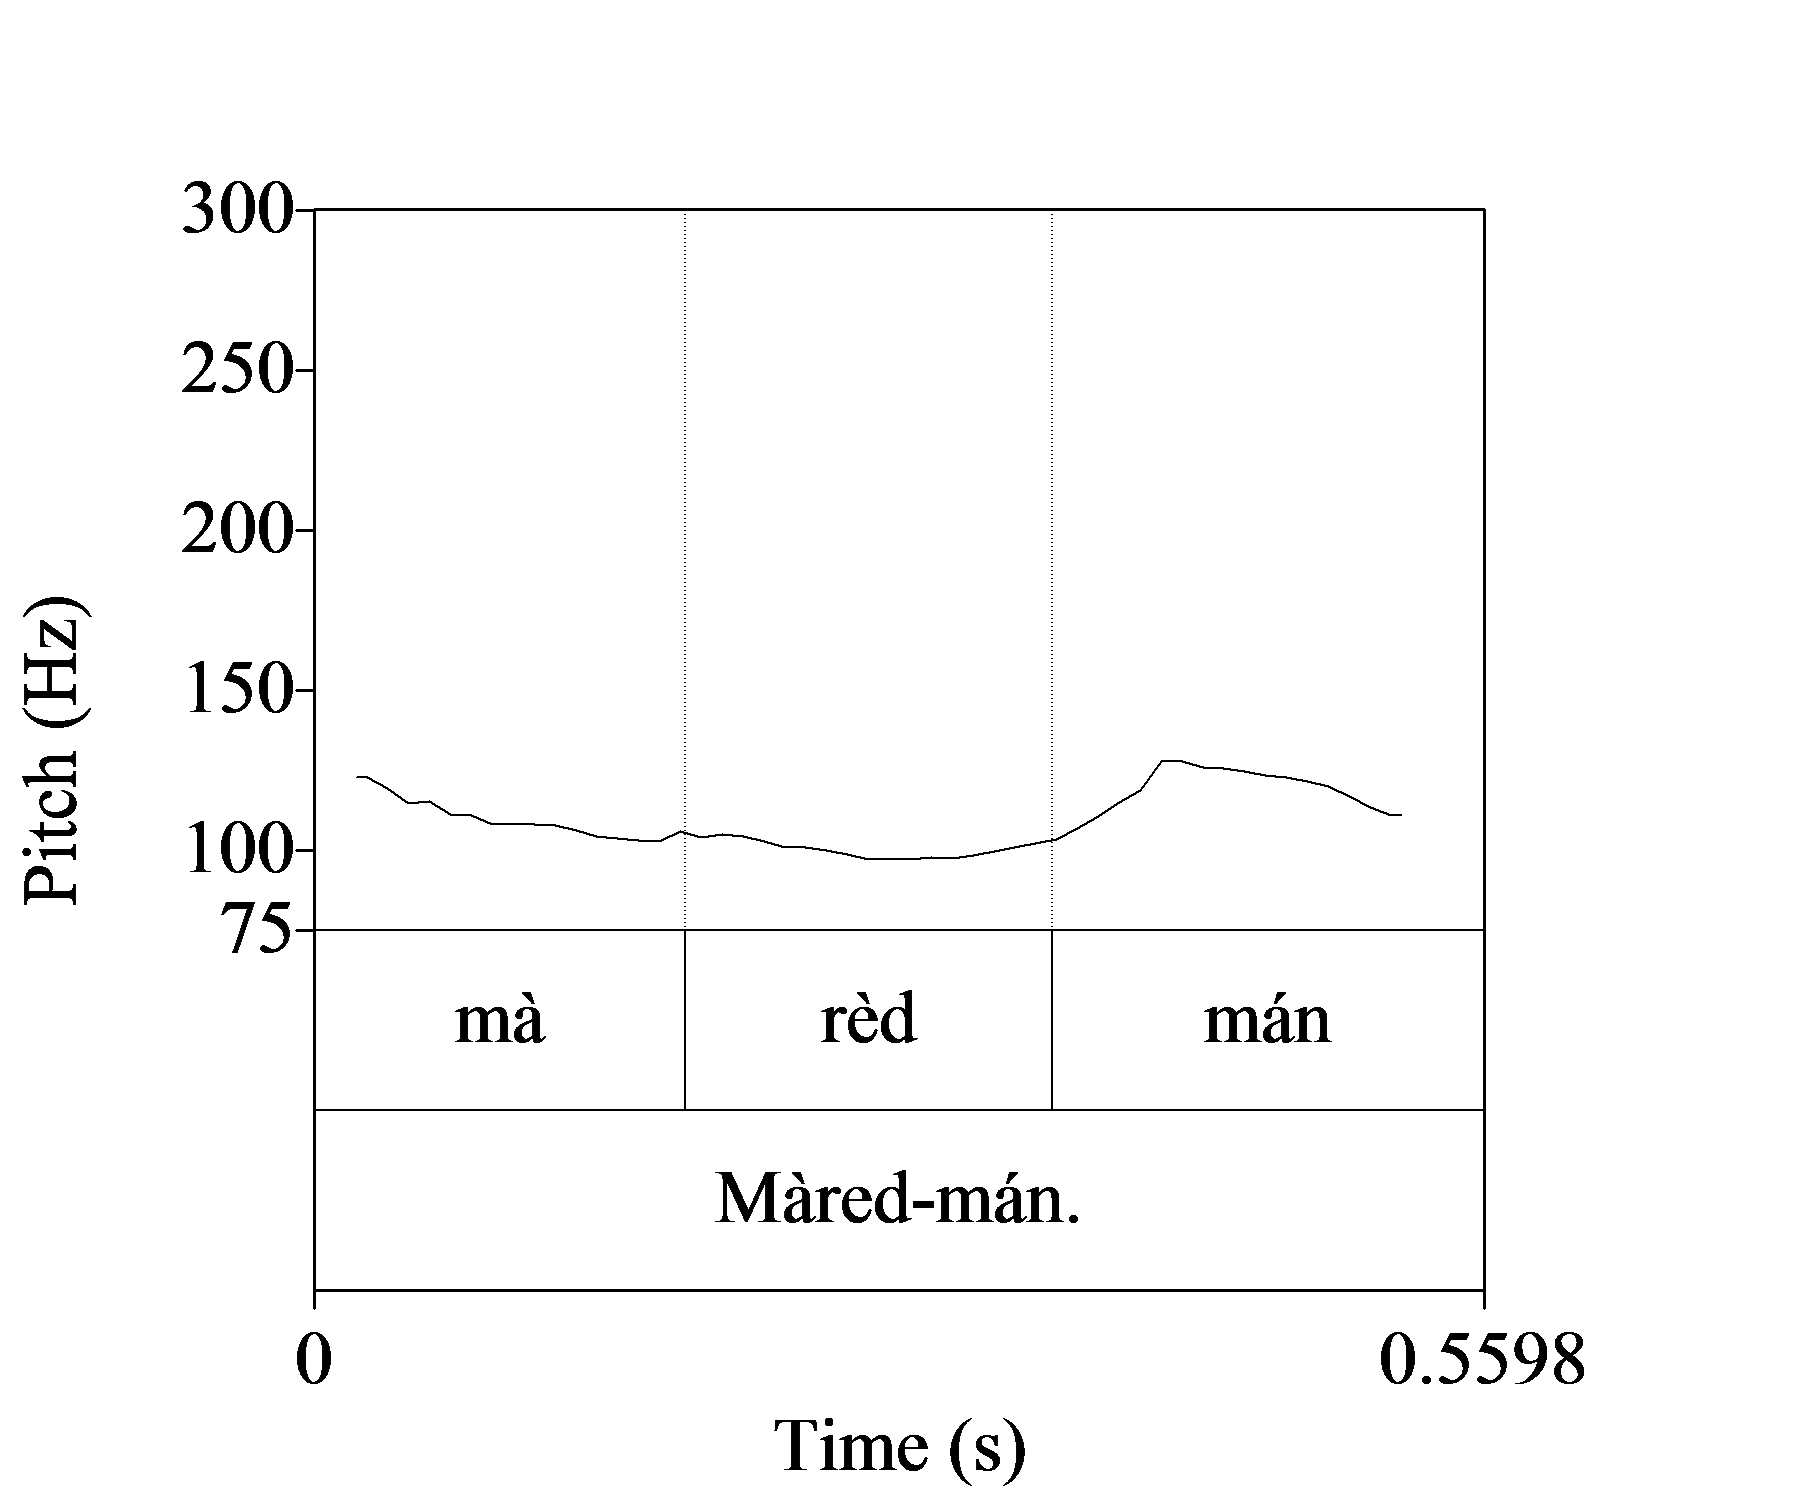
\includegraphics[height=.3\textheight]{figures/yakpomod-img22.png} 
\end{figure}

\ea\label{ex:key:58}
\glll   Fúlis  mán.\\
\textsc{h.h}    \textsc{h}\\
foolish  man\\
\glt   ‘Foolish man.’ 
\z
\ea\label{ex:key:59}
\glll    \textstylePichiexamplebold{Mared}{}-mán\\
\textbf{\textsc{l}}.\textsc{l-h}\\
marry.\textsc{cpd}{}-man.\\
\glt ‘Married man.’
\z
In contrast, the pitch trace in \figref{fig:key:3.20} above exemplifies tone deletion. The head noun \textit{mán} ‘man’ is also modified by a verb with an H.L pattern, namely \textit{máred} ‘marry; be married’. However, \textit{máred} and \textit{mán} form a single phonological word, the compound noun \textit{mared-mán} ‘married man’. The H tone over the first syllable of \textit{máred} has been deleted in the process and replaced by L (the downward cline over the first syllable is caused by a pitch reset at the beginning of the utterance). At the same time, \textit{mán}, the final component of the compound, retains its H tone (which falls slightly due to its utterance-final position).


Reduplicated verbs exhibit the same suprasegmental characteristics as compound nouns. The pitch trace of the reduplicated (and sentence-medial) monosyllabic \textit{rɔ́n} ‘run’ in \figref{fig:key:3.21} shows an L.H pitch configuration over the two identical components. This parallels the pitch trace over the compound \textit{wach-mán} ‘watchman’ above. Reduplication therefore involves the same derivational process as compounding: The lexical H-tone over the first component is deleted and replaced by an L tone: 


\begin{figure}
\caption{Monosyllabic reduplicated verb}
\label{fig:key:3.21}
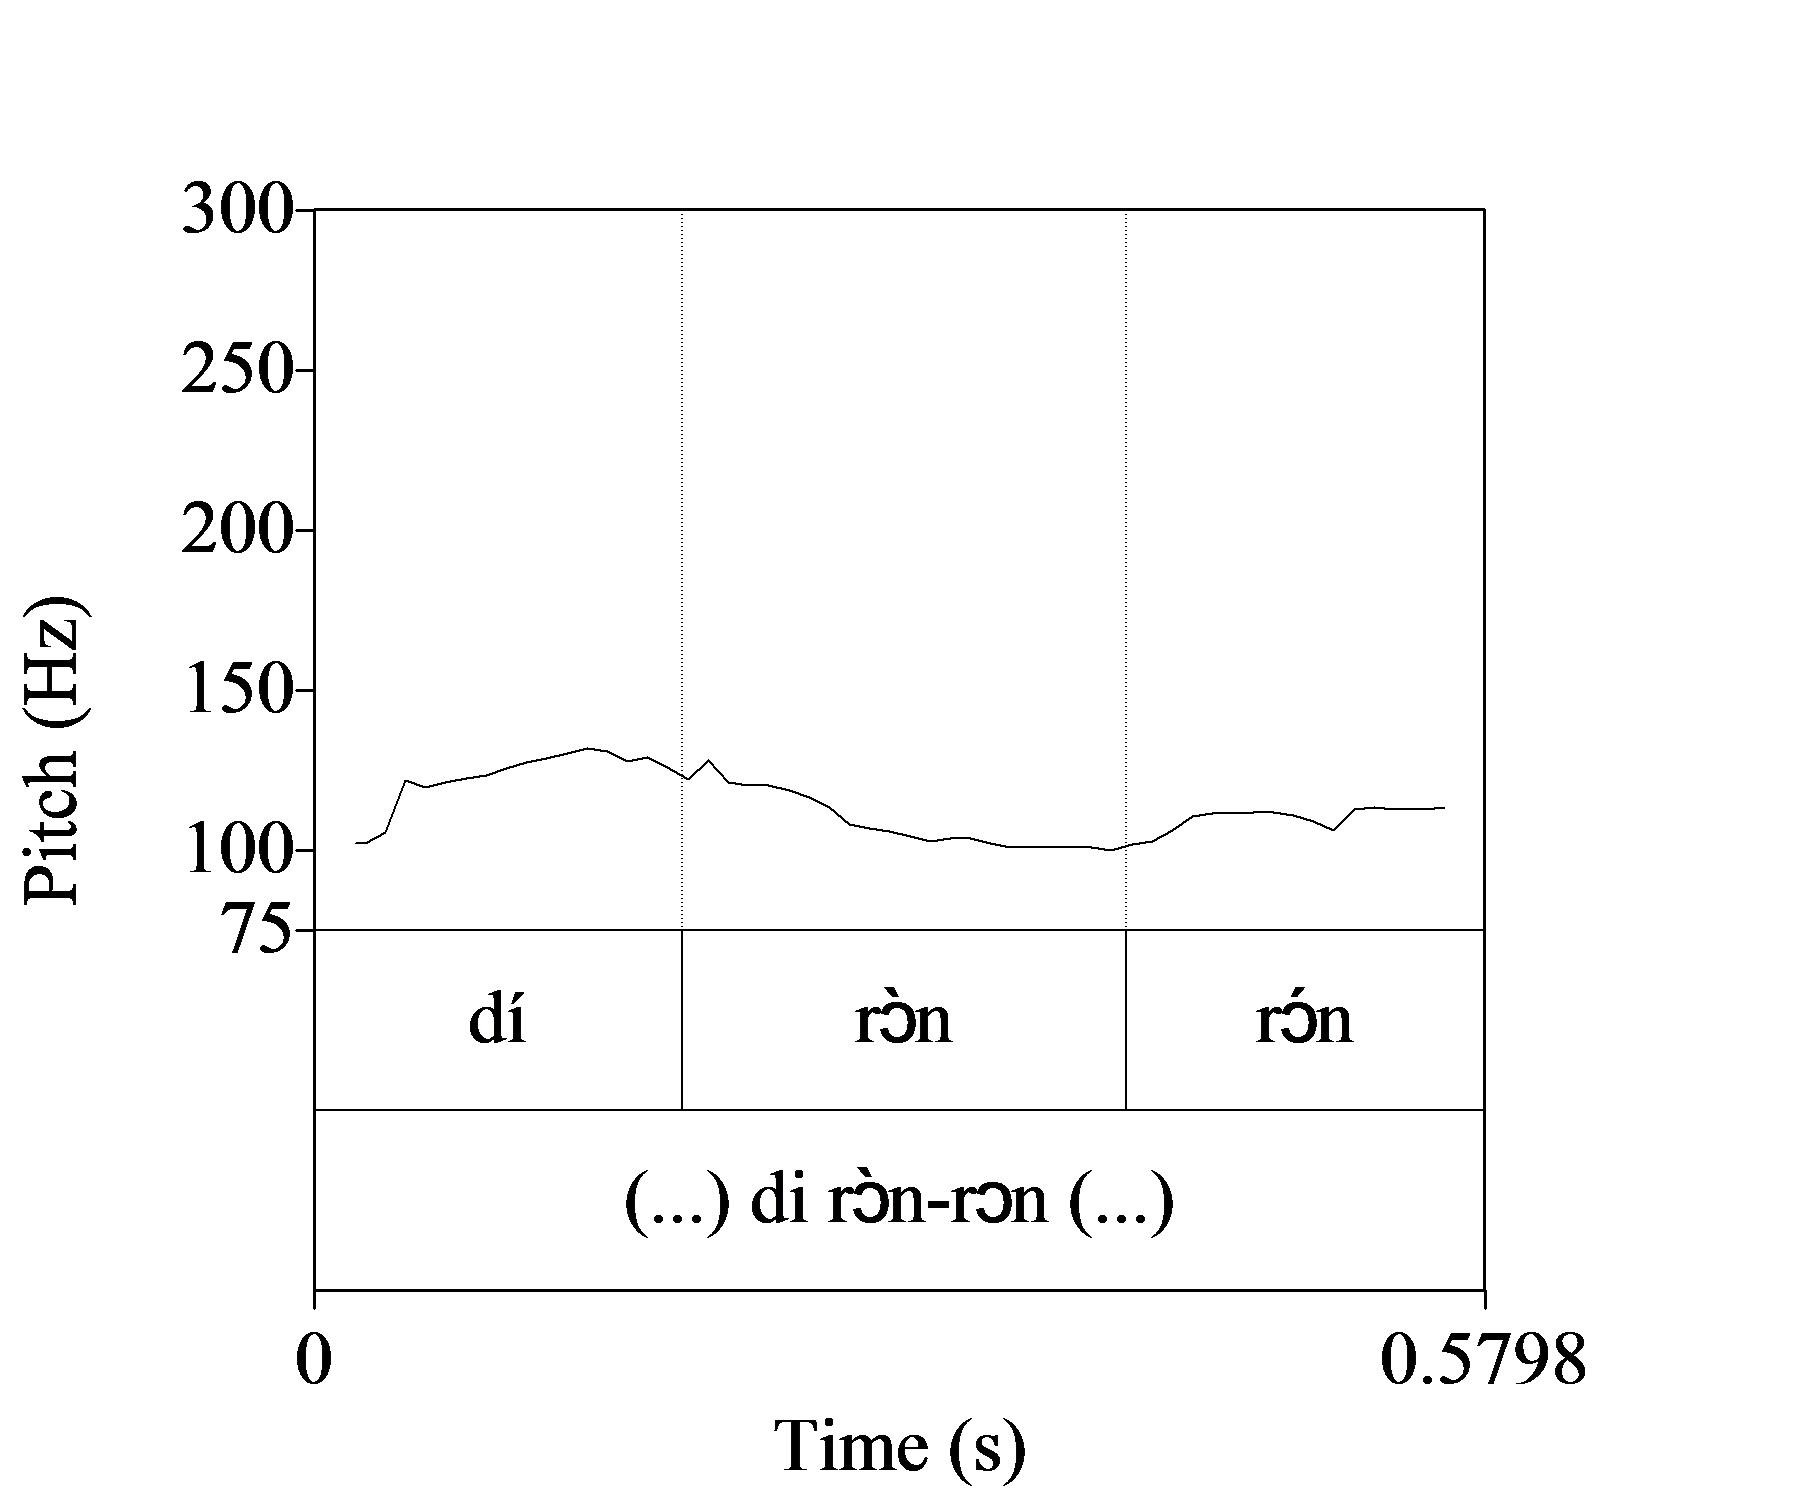
\includegraphics[height=.3\textheight]{figures/yakpomod-img23.png}
\end{figure}

\begin{figure}
\caption{Bisyllabic reduplicated verb}
\label{fig:key:3.22} 
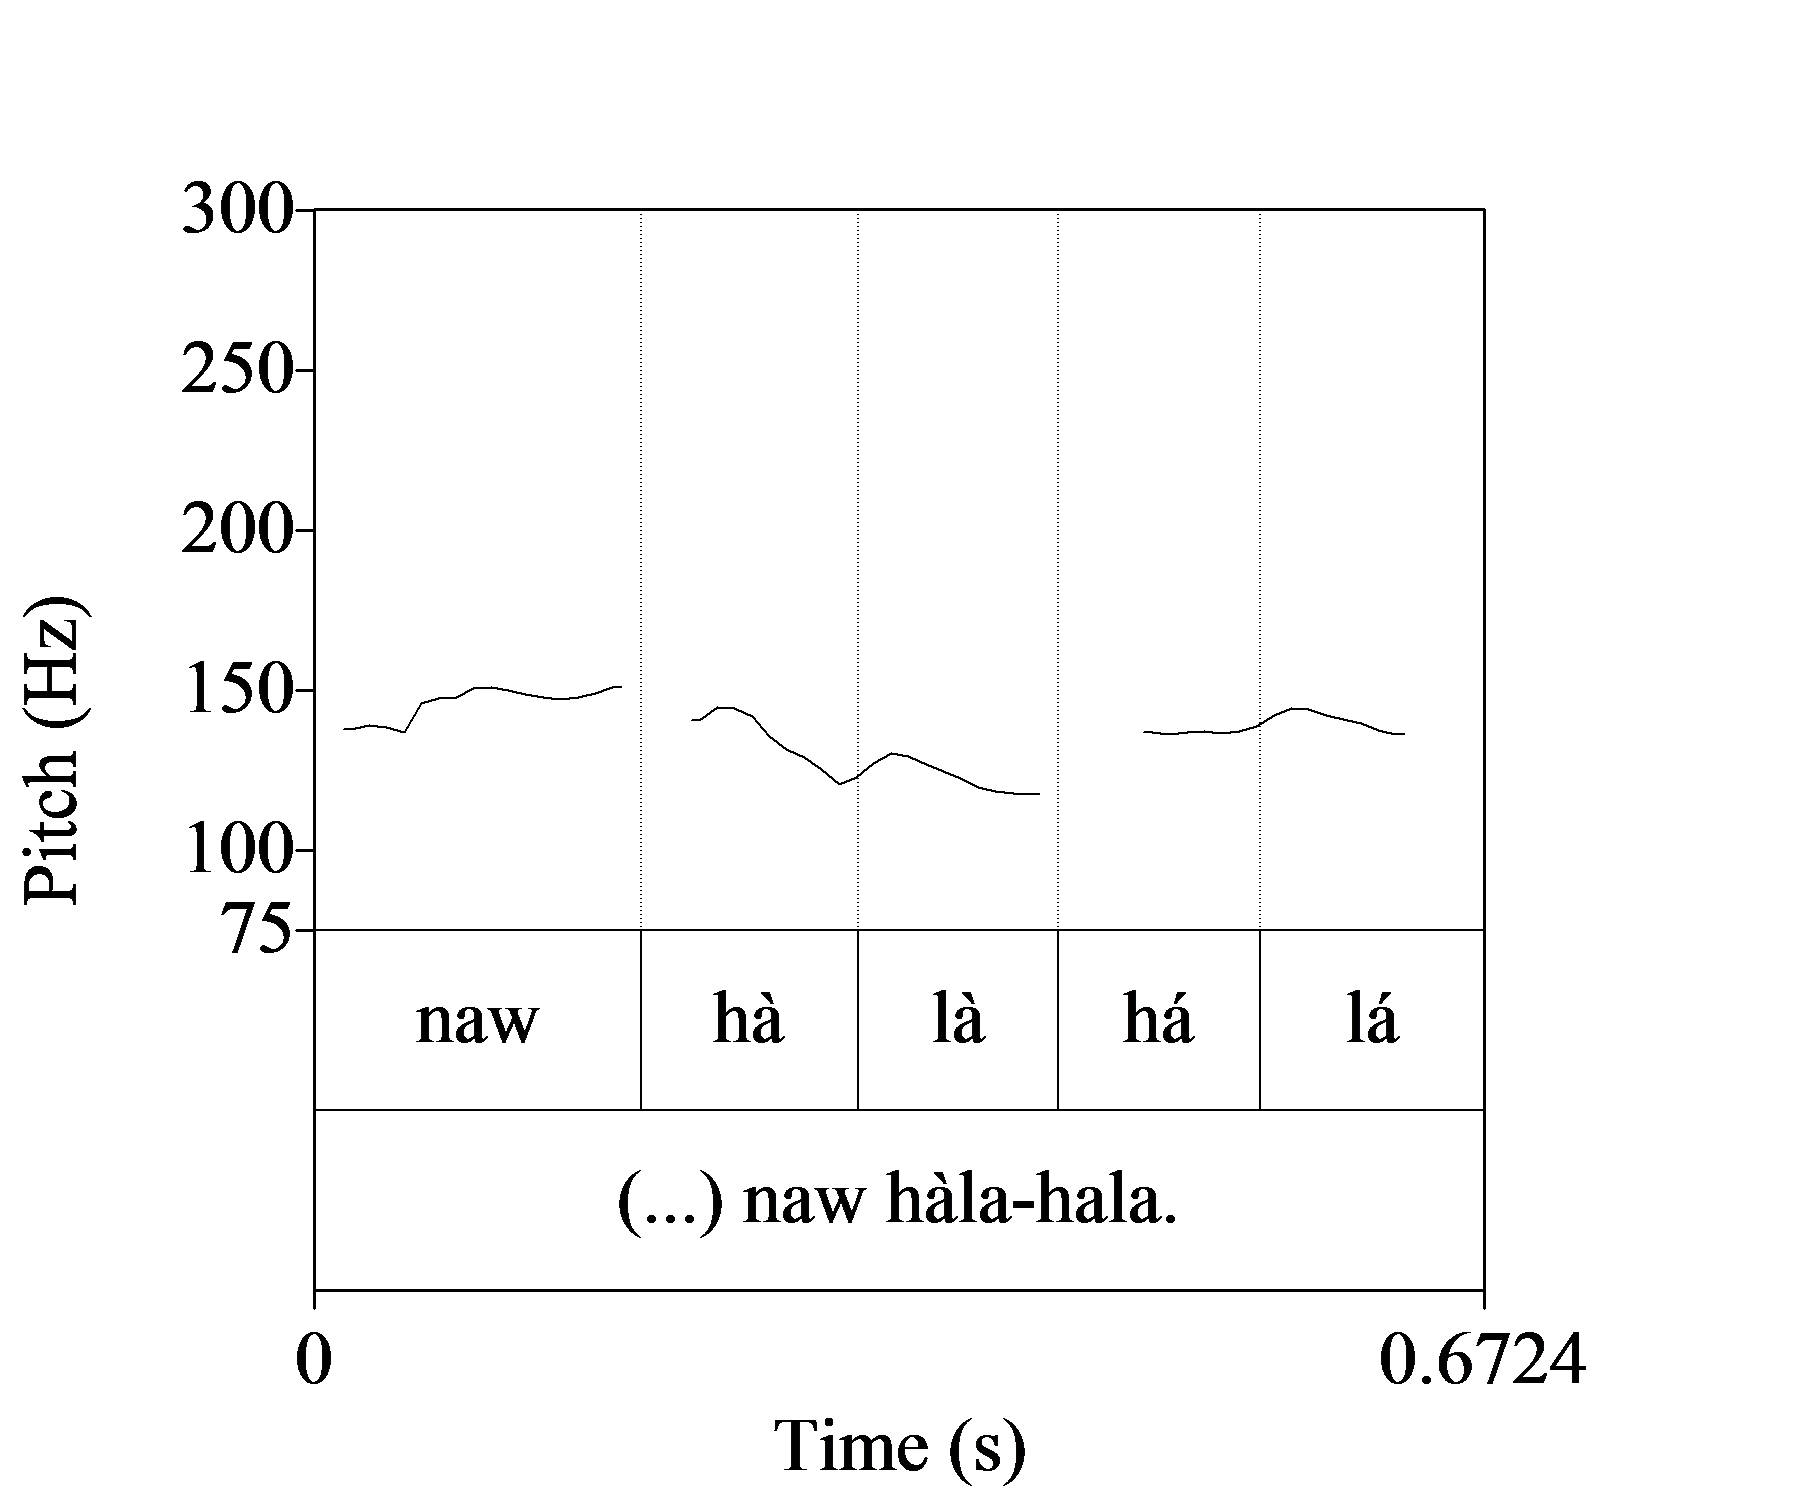
\includegraphics[height=.3\textheight]{figures/yakpomod-img24.png} 
\end{figure}
 
\ea%60
    \label{ex:key:60}
    \gll   Dí  \textstylePichiexamplebold{rɔn-}rɔ́n (…)\\
\textsc{h}  \textstylePichiexamplebold{\textsc{l}}\textsc{{}-h}\\
this  \textsc{red.cpd-}run\\
\glt ‘This running around (…)’
\z

\ea
	\label{ex:key:61}
\gll    Náw    \textstylePichiexamplebold{hala}{}-hála.\\
\textsc{h}    \textstylePichiexamplebold{\textsc{l}}\textstylePichiexamplenumberZchnZchn{.}\textstylePichiexamplenumberZchnZchn{\textsc{l}}\textsc{{}-h.h}\\
now    \textsc{red.cpd}{}-shout\\
\glt ‘Now, (it was) constant shouting.’\\
\z

\subsection{Pitch range expansion}\label{sec:3.2.5}

In Pichi, certain phonetic features may increase the prominence of a (series of) syllable(s). Segments may be lengthened or may be pronounced with increased volume, they may be pronounced with a breathy or creaky voice, and the speech rate may be slowed down or accelerated for stylistic effect. But there is no stress in Pichi in the sense of an automatic, metrically conditioned culmination of phonetic features as in intonation-only languages. Nor does Pichi make use of intonational melodies spanning the entire (or parts of the) utterance for the realisation of pragmatic functions, since these would override the lexical tone of individual words. Instead, pitch range expansion, and an extra-high tone in particular, are exploited to signal focus and emphasis. Focused or emphasised constituents may bear a higher than usual pitch, an extra-high tone on their H-toned syllable(s). The extra-high tone may spread rightwards onto following L-toned syllables until the word boundary is reached (cf. \sectref{sec:3.2.1}). 

\figref{fig:key:3.23} features the clefted verb \textit{drɔ́ngo} ‘be dead drunk’. In the pitch trace, the emphatic character of the predicate cleft construction \is{predicate cleft}is evident in two ways. The H-toned syllable of \textit{drɔ́ngo} bears an extra-high tone, and the segment /r/ is lengthened for emphasis. The utterance in \figref{fig:key:3.23} shades off into a chuckle from the fifth syllable onwards, which produces a wavering pitch trace:

\begin{figure}
\caption{Predicate cleft and extra-high tone for emphasis}
\label{fig:key:3.23}
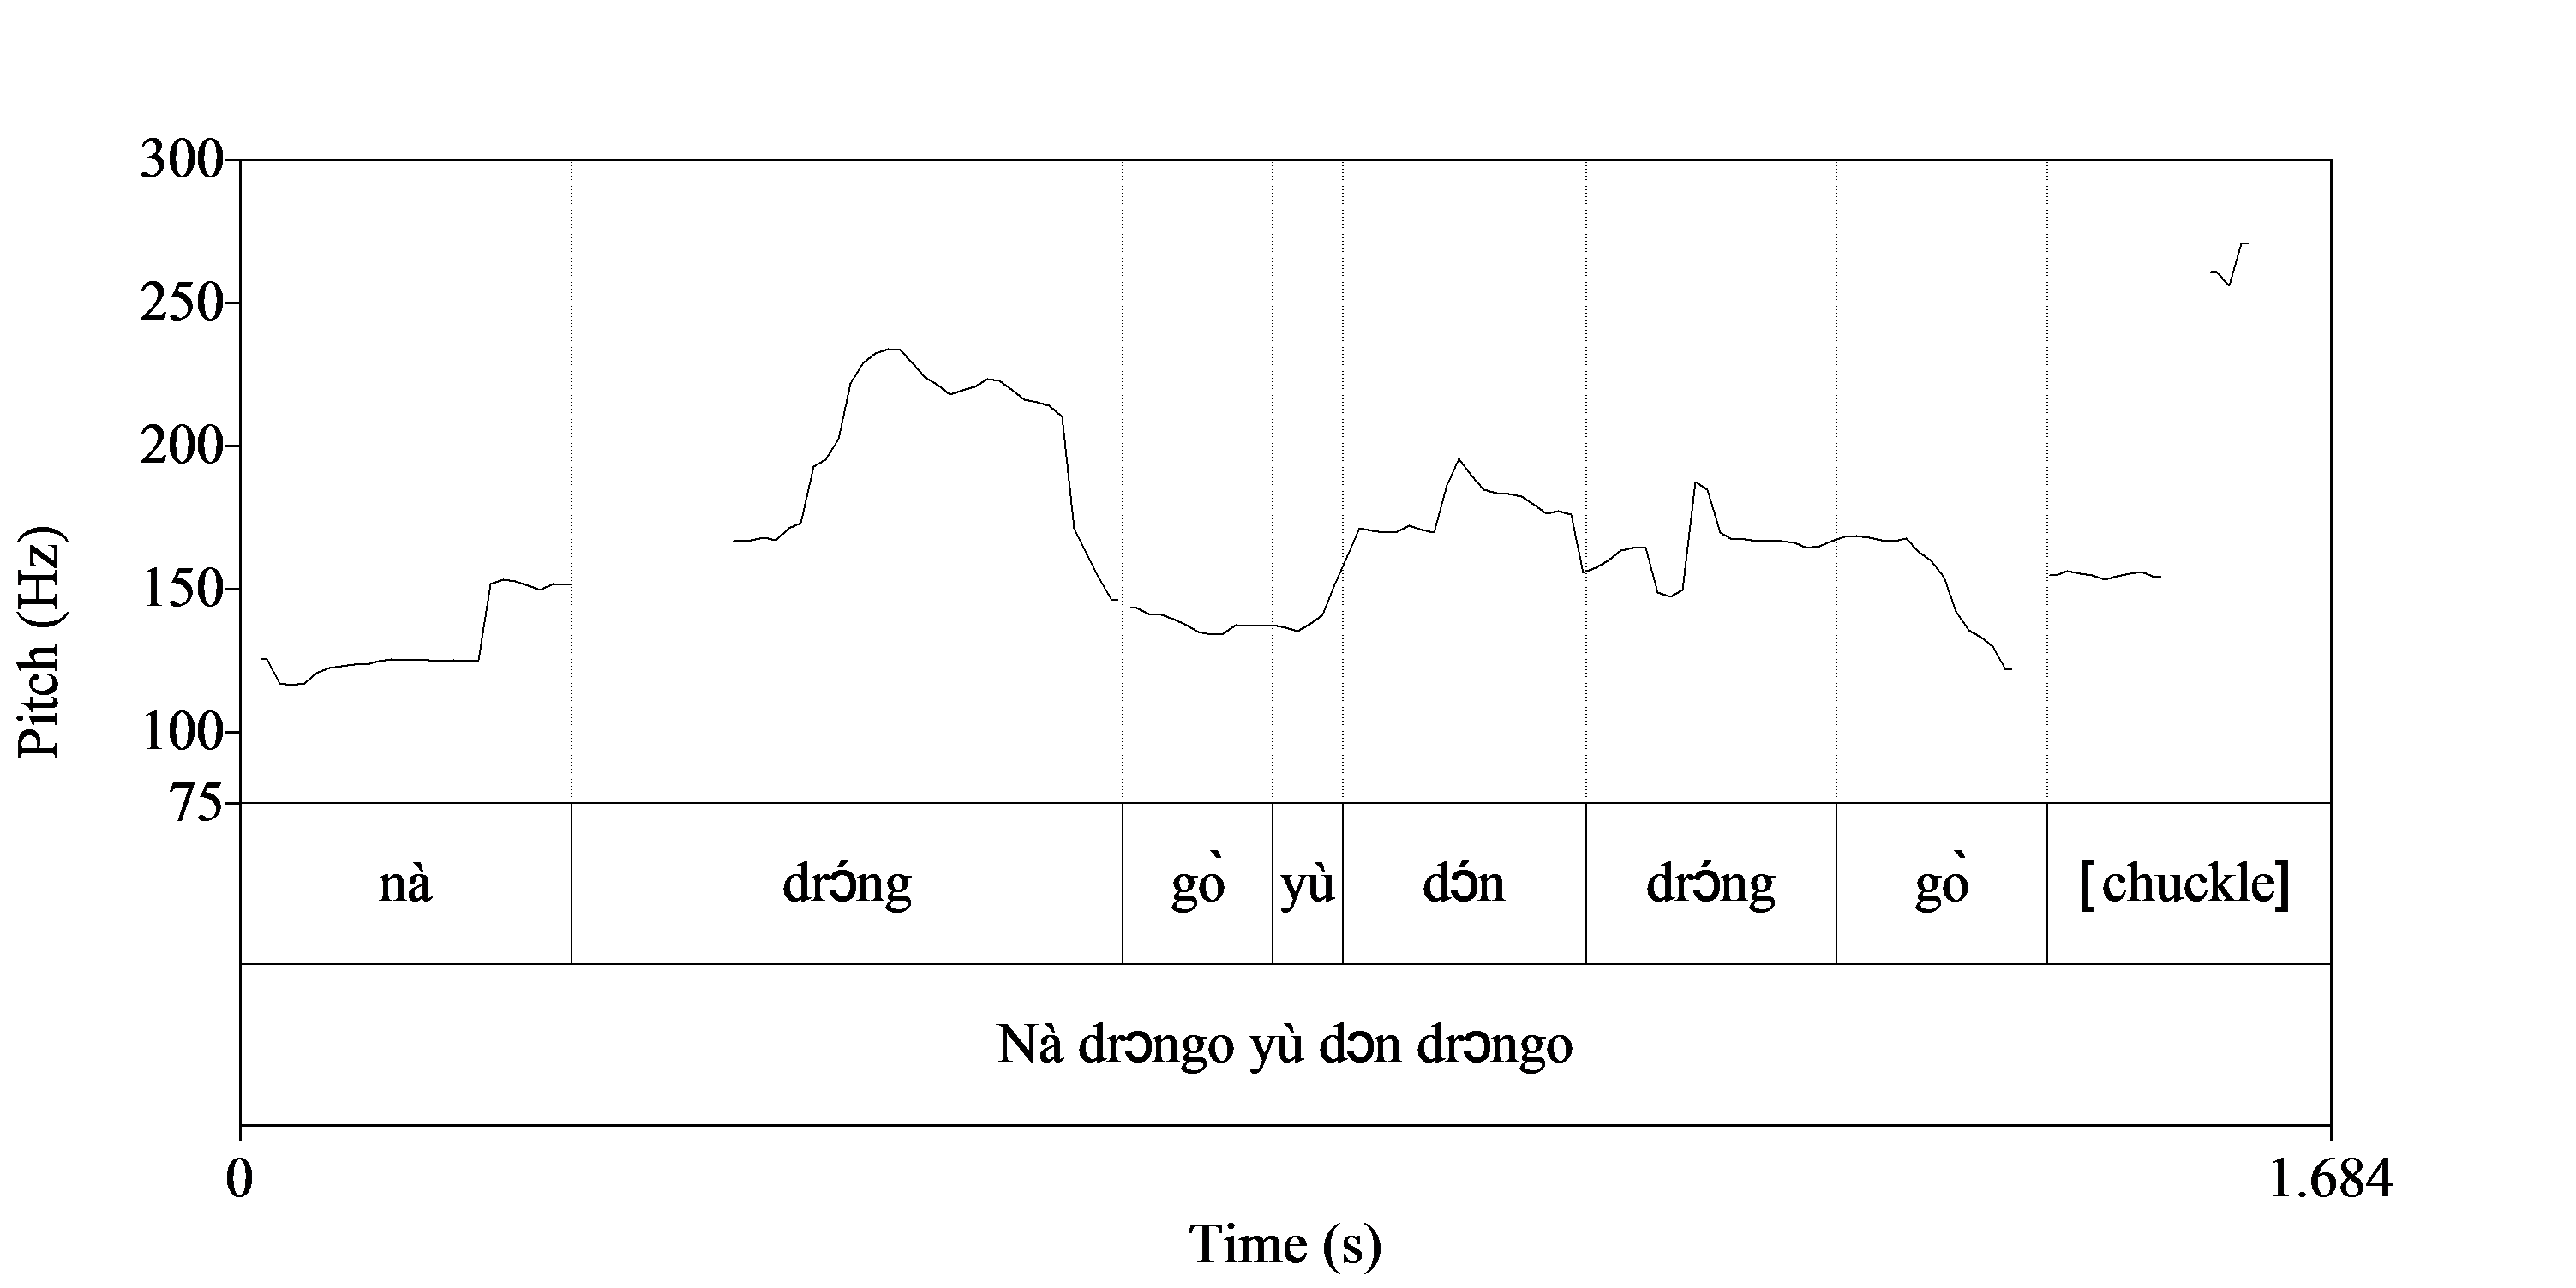
\includegraphics[height=.3\textheight]{figures/yakpomod-img25.png}
\end{figure}
 


\ea%62
    \label{ex:key:62}
    \glll   Na  [\textstylePichiexamplebold{drrrɔ́ngò}]    yu  dɔ́n  drɔ́ngo. \\
\textsc{l}  \textbf{\textsc{+h}}\textsc{.l}        \textsc{l}  \textsc{h}  \textsc{h.l}\\
\textsc{foc}  be.dead.drunk  \textsc{2sg}  \textsc{prf}  be.dead.drunk\\
\glt ‘You’re absolutely dead drunk.’     
\z

Elements that fulfil central functions in pragmatically marked contexts are particularly common with extra-high tone, e.g. question elements like \textit{háw} ‘how’, \textit{wétin} ‘what’, \textit{údat} ‘who’, \textit{ús=tín}  ‘what’, the negator \textit{nó}\is{negation}, modifications of degree via repetition\is{repetition} like \textit{bíg bíg} ‘very big’, and the degree adverb \textit{bád} ‘bad, extremely’. Both components of the repetition \textit{bíg bíg} ‘be very big’ in \figref{fig:key:3.24} below carry an extra-high tone. There is no sign of downstep\is{downstep} within the reduplicated sequence: 

\begin{figure}
\caption{Extra-high tone}
\label{fig:key:3.24}
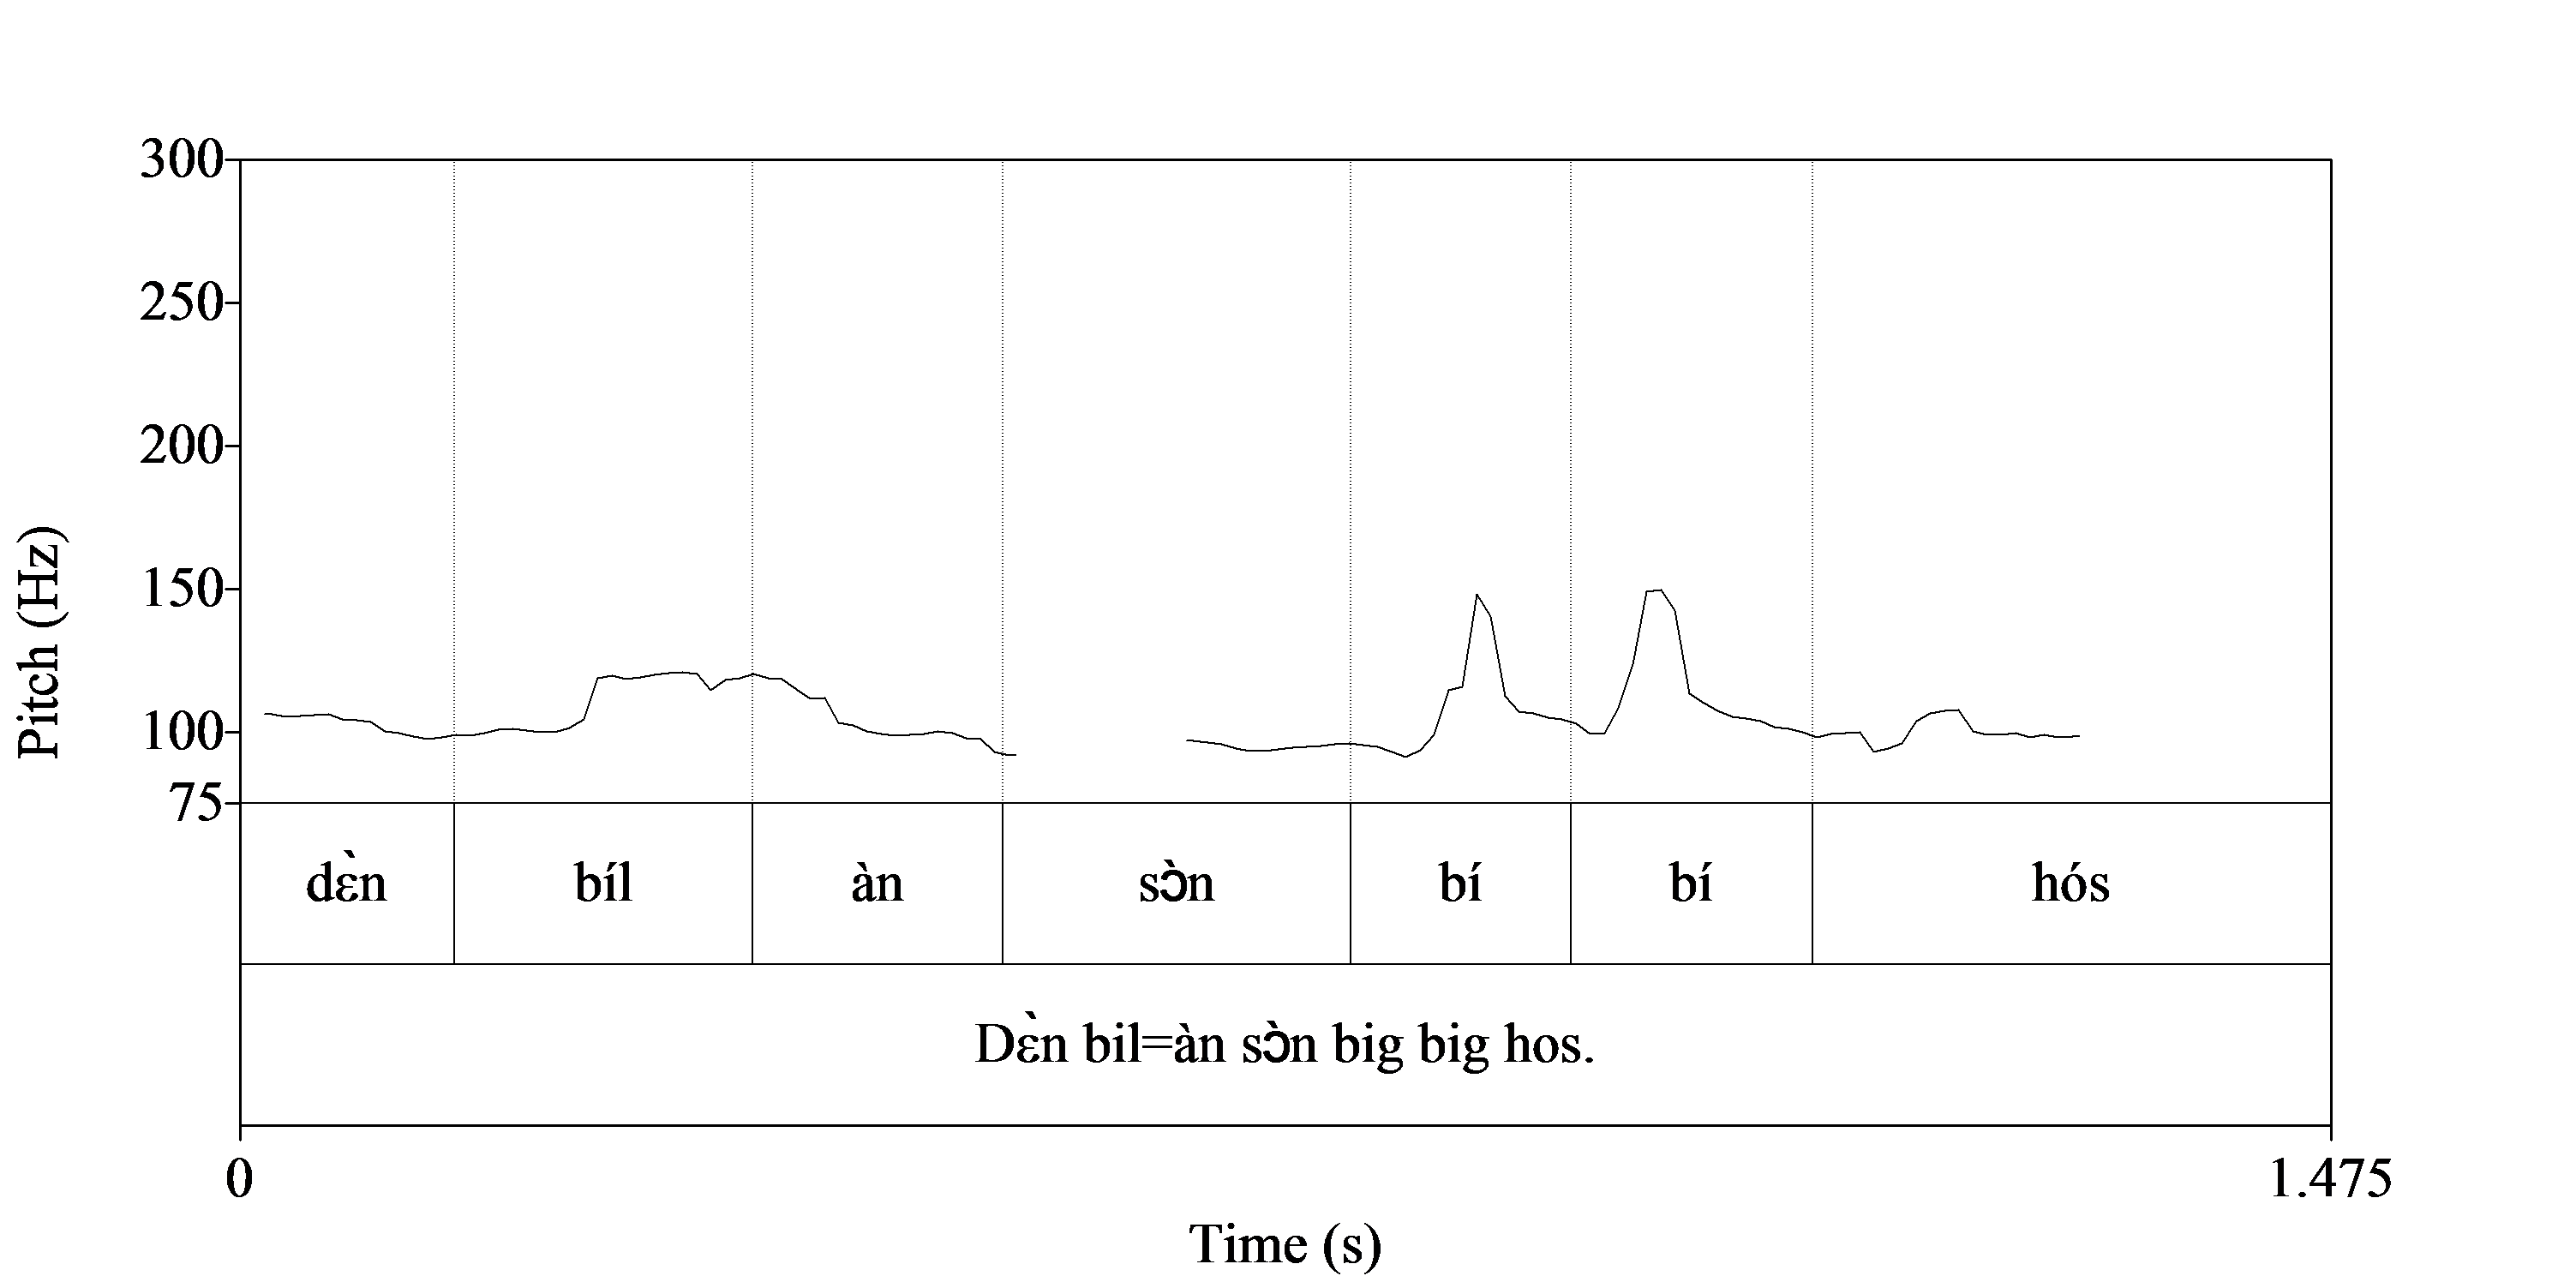
\includegraphics[height=.3\textheight]{figures/yakpomod-img26.png}
\end{figure}
 


\ea%63
    \label{ex:key:63}
    \glll   Dɛn    bíl=an    sɔn    \textstylePichiexamplebold{bíg}  \textstylePichiexamplebold{bíg}    hós.\\
\textsc{h}    \textsc{h=l}      \textsc{l}    \textbf{\textsc{+h}  \textbf{+h}}    \textsc{h}\\
\textsc{3pl}    build=\textsc{3sg.obj}  some  big  \textsc{rep}    house\\
\glt ‘They built him a huge house.’    
\z

Entire clauses or sentences may also be placed under focus \is{prosodic focus} by (a series of) extra-high tones, which thereby (cumulatively) fulfil(s) the same function as emphatic intonation covered in \sectref{sec:3.4.2} further below. There are two principal means of emphasising sentences, which are often used together. The last H tone of the utterance may be raised to an extra-high pitch as in \figref{fig:key:3.25}. Here the H tone of the utterance-final word \textit{mán} ‘man’ has been raised to an extra-high level. The sentence nonetheless bears declarative intonation. The word \textit{mán} still exhibits the utterance-final fall characteristic of declarative intonation (cf. \sectref{sec:3.4.1}) but at a significantly higher pitch level than in a non-emphatic context:

\begin{figure}
\caption{Utterance-final extra-high tone for emphasis\is{emphasis}}
\label{fig:key:3.25}
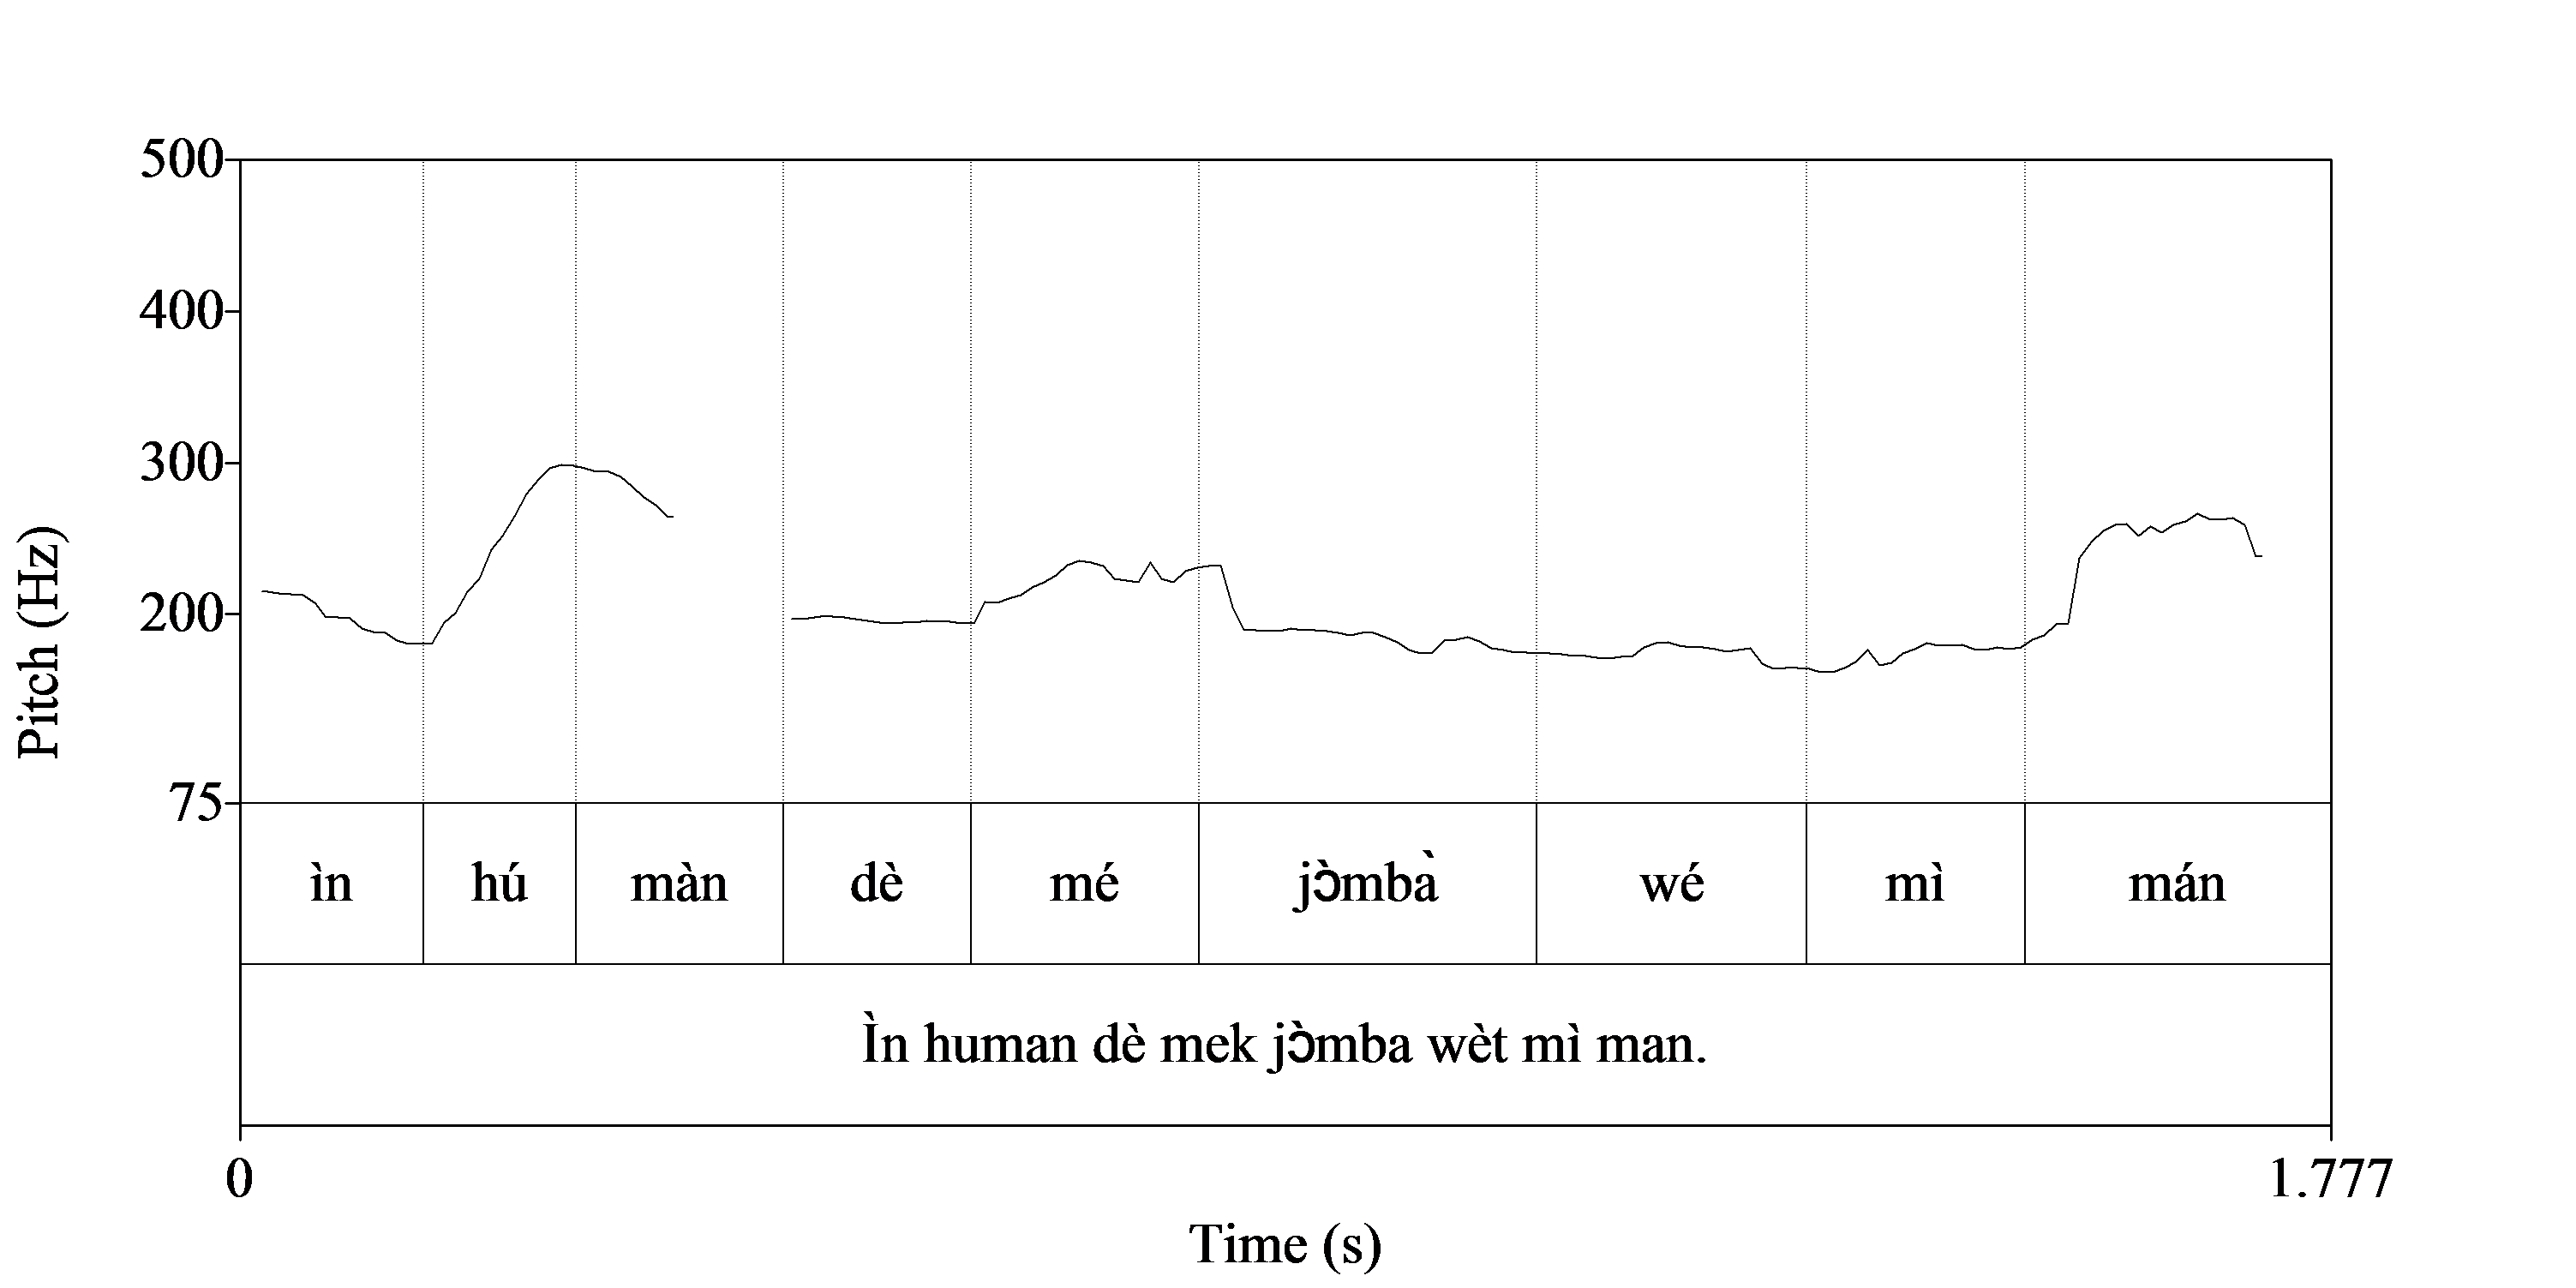
\includegraphics[height=.3\textheight]{figures/yakpomod-img27.png}
\end{figure}
 


\ea%64
    \label{ex:key:64}
    \glll   Yu  húman  de  mék    jɔmba  wet  mi    \textstylePichiexamplebold{mán}.\\
\textsc{l}  \textsc{h.l}    \textsc{l}  \textsc{h}    \textsc{l.l}    \textsc{l}  \textsc{l}    \textbf{\textsc{+h}}\textsc{l\%}\\
\textsc{2sg}  woman  \textsc{ipfv}  make  affair  with  \textsc{1sg.poss}  man.\\
\glt ‘Your wife is having an affair with my husband.’
\z

Secondly, the use of an utterance-final extra-high tone is often accompanied by “pitch range expansion” \citep[276]{Yip2002}. Alternatively, pitch range expansion may be accompanied by the use of the emphatic boundary tone instead of the utterance-final extra-high tone (cf. \sectref{sec:3.4.2}). During pitch range expansion, the pitch range between H and L tones is widened throughout the entire utterance by pronouncing H tones with a higher-than-usual pitch and, optionally, L tones with a lower-than-usual pitch. This creates a strongly undulating pitch contour over the entire utterance.

\figref{fig:key:3.26} graphically depicts the dramatic rises and falls that may characterise pitch range expansion. The female speaker begins with an L-toned \textit{na} at 190 Hz, rises to 490 Hz with H-toned \textit{só}, then falls to an all-time low with \textit{dɛn} at 145 Hz, until the pitch range gradually evens out towards the end of the utterance:

\begin{figure}
\caption{Pitch range expansion for emphasis\is{emphasis}}
\label{fig:key:3.26}
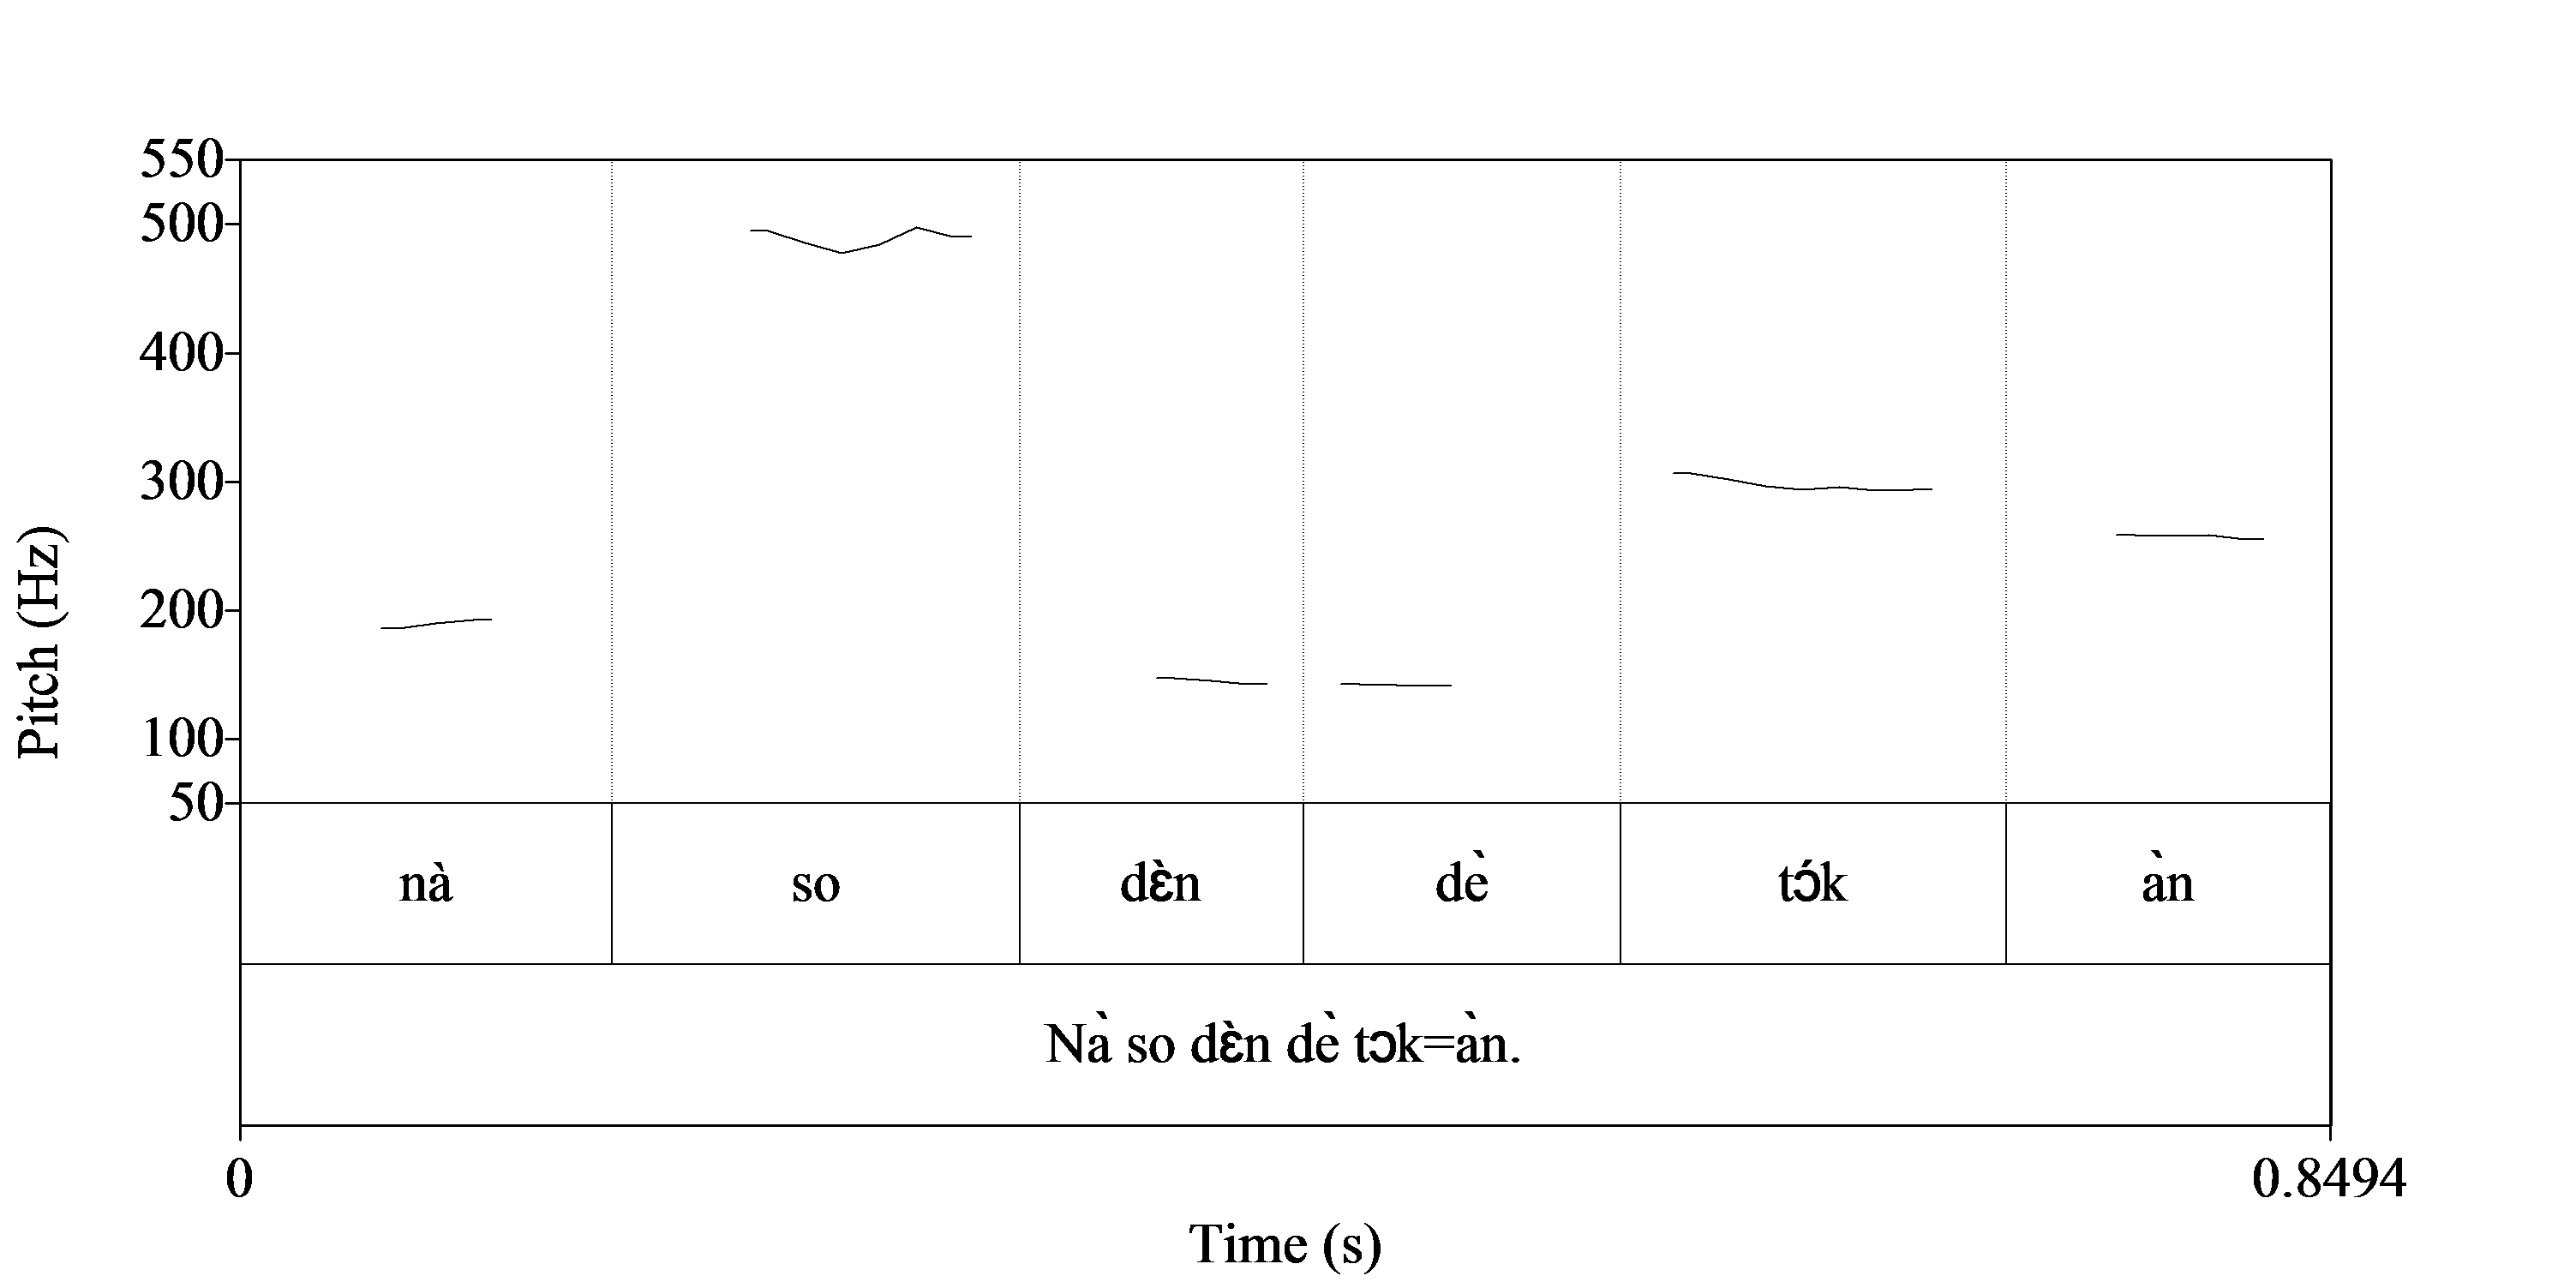
\includegraphics[height=.3\textheight]{figures/yakpomod-img28.png}
\end{figure}
 


\ea%65
    \label{ex:key:65}
    \glll   Na  \textstylePichiexamplebold{só}    \textbf{dɛn}  \textbf{de}  \textbf{tɔ́k}=an.    \\
\textsc{l}  \textbf{\textsc{+h}    \textbf{+l}  \textbf{+l}  \textbf{+h}}\textsc{=lh\%}      \\
\textsc{foc}  like.that  \textsc{3pl}  \textsc{ipfv}  talk=\textsc{3sg.obj}\\
\glt ‘That’s how they say it.’
\z

\section{Tone-conditioned suppletive allomorphy}\label{sec:3.3}

Pichi features a tone-conditioned suppletive allomorphy (TCSA) of the two pronominal variants \textit{=an} \textsc{‘3sg.obj’} and \textit{ín} ‘\textsc{3sg.indp’}, which may both instantiate (direct and indirect) object case (cf. \sectref{sec:5.4.1} for an overview of the inflection of personal pronouns). Suppletive allomorphy is conditioned by a tonotactic prohibition of immediately adjoining or “string-adjacent” \citep{Suzuki1998} identical tones (cf. also \sectref{sec:2.6.2.2}). Suppletive allomorphy therefore relies on the conditioning environment of vowel hiatus. Further, there are no phonemic long vowels in Pichi. String-adjacent vowels within the same lexical word are always heterosyllabic, and in addition, invariably carry polar tones (cf. \sectref{sec:2.6.2.2}). TCSA can therefore only be triggered when the enclisis of \textit{=an} \textsc{‘3sg.obj’} creates a phonological word. A head with an L-toned vowel-final syllable may therefore not take the vowel-initial L-toned clitic object pronoun \textit{=an}. Instead, the independent (emphatic) personal pronoun \textit{ín} \textsc{‘3sg.indp’} is recruited as a suppletive allomorph. Allomorph distribution according to the phonological class of the host is summarised in \tabref{tab:key:3.4}:

%%please move \begin{table} just above \begin{tabular
\begin{table}
\caption{Distribution of suppletive object pronouns}
\label{tab:key:3.4}

\begin{tabularx}{.8\textwidth}{XXl}
\lsptoprule
{Host class} & {Allomorph} & {Example}\\
\midrule
C/{\longrule}\# & =an & [márè\textbf{d}=àn]\\
\'{V}/{\longrule}\# & =an & [tròw\textbf{é}=àn]\\
\`{V}/{\longrule}\# & ín & [fíb\textbf{à} ín]\\
\lspbottomrule
\end{tabularx}
\end{table}

There is no tonotactic restriction on the enclisis of \textit{=an} with consonant-final hosts like \textit{máred} ‘marry’, since the condition of tonal string-adjacency is not met: 


\ea%66
    \label{ex:key:66}
    \gll   E    go  máre\textbf{d}=\textbf{an}.\\
\textsc{3sg.sbj}  \textsc{pot}  marry=\textsc{3sg.obj}\\

\glt ‘S/he’ll marry him/her.’ 
\z

There are no restrictions on the enclisis of \textit{=an} with vowel-final hosts with a word-final H-tone like \textit{trowé} ‘throw, pour away’, since the vowel sequence across the morpheme boundary bears a polar [H.L] tone:


\ea%67
    \label{ex:key:67}
    \gll   A    fít  ték    di  wɔtá  a    trow\textbf{é}=\textbf{an}.\\
\textsc{1sg.sbj}  can  take    \textsc{def}  water  \textsc{1sg.sbj}  throw=\textsc{3sg.obj}\\

\glt ‘I can take the water (and) pour it away.’ 
\z

If the word-final vowel of the host is L-toned, as with \textit{fíba} ‘resemble’, the pitch configuration after enclisis of \textit{=an} across the clitic boundary would be [L.L]. This is an illicit pitch configuration over string-adjacent vowels in Pichi phonological words and triggers the use of suppletive \textit{ín} ‘\textsc{3sg.indp’.} Compare the following two examples:


\ea%68
    \label{ex:key:68}
    \gll   \textit{*}Yu    fíb\textbf{a}=\textbf{an}    bɔkú.\\
\textsc{2sg}  resemble=\textsc{3sg.obj}  a.lot\\

\glt  ‘You resemble him a lot.’ 
\z


\ea%69
    \label{ex:key:69}
    \gll   Yu  \textbf{fíba}      \textbf{ín}    bɔ́ku.\\
\textsc{2sg}  resemble    \textsc{3sg.indp}  a.lot\\

\glt ‘You resemble him/her a lot.’ 
\z

The class of words that features the allomorph \textit{ín} as an object pronoun also includes verbs of Spanish origin. Spanish verbs are always inserted into Pichi clauses in the Spanish \textsc{3sg} present tense form, irrespective of their tense-aspect (cf. \sectref{sec:13.2.2}). Examples follow with the verbs \textit{fírma} ‘sign’ (< Span. \textit{firmar}) from the Spanish 1\textsuperscript{st} conjugation class, and \textit{sube} ‘go/bring up’ (< Span. \textit{subir}) from the 3\textsuperscript{rd} conjugation class:


\ea%70
    \label{ex:key:70}
    \gll   Dɛn    nó    \textbf{fírma}  \textbf{ín}    yét.    \\
\textsc{3pl}    \textsc{neg}    sign    \textsc{3sg.indp}  yet\\


\glt ‘They haven't signed it yet.’\\

\z

\ea%71
    \label{ex:key:71}
    \gll   Dán    mán    go  \textbf{súbe}  \textbf{ín}.\\
that    man    \textsc{pot}  bring.up  \textsc{3sg.indp}\\

\glt ‘That man will bring it [the suitcase] up.’
\z

Pichi has a second mechanism next to tone-conditioned suppletive allomorphy to ensure that the requirement of a string-adjacent polar [H.L] tone is not breached. A buffer consonant /r/ can be inserted at the clitic boundary. Epenthesis forestalls the cross-morphemic vowel hiatus and makes the use of the allomorph \textit{ín} unnecessary:


\ea%72
    \label{ex:key:72}
    \gll   Yu  fíba[\textbf{r}]=\textbf{an}    bɔkú.\\
\textsc{2sg}  resemble=\textsc{3sg.obj}  a.lot\\

\glt ‘You resemble him a lot.’ 
\z

Once the epenthetic segment is present, there is no phonotactic difference with a word in which the final consonant forms an integral part of the root like \textit{máred} ‘marry’ in \REF{ex:key:66}. Another example featuring epenthesis follows, involving the general associative preposition \textit{fɔ} ‘\textsc{prep}’. In \REF{ex:key:73}, we find /r/ epenthesis, in \REF{ex:key:74}, suppletive allomorphy:


\ea%73
    \label{ex:key:73}
    \gll   E    tót=an    fɔ[\textbf{r}]=\textbf{an}.\\
\textsc{3sg.sbj}  carry=\textsc{3sg.obj}  \textsc{prep=3sg.obj}\\

\glt ‘He carried it for her.’
\z


\ea%74
    \label{ex:key:74}
    \gll   Dán    tín    dé    \textbf{fɔ}  \textbf{ín}.\\
that    thing  \textsc{be.loc}  \textsc{prep}  \textsc{3sg.indp}\\

\glt ‘That thing is hers.’
\z

Three aspects are noteworthy with respect to /r/ epenthesis in Pichi. Firstly, /r/ insertion is exceedingly rare in natural discourse. In the Pichi corpus, there are less than a dozen instances of /r/ epenthesis in natural discourse, involving a mere handful of lexemes, among them \textit{kɔ́ba[r]=an} ‘cover it’, \textit{klía[r]=an} ‘clear it’, \textit{fía[r]=an} ‘fear him/her’, \textit{fíba[r]=an} ‘resemble him/her, \textit{drɔ́ngo[r]=an} ‘get him/her drunk’, and \textit{fɔ[r]=an} ‘for him/her’. By contrast, the corpus contains hundreds of syntagmas involving the suppletive allomorph \textit{ín.} I could therefore only uncover the distribution of the epenthetic /r/ and its role in TCSA by means of elicitation. Secondly, elicitation revealed that the availability of /r/ epenthesis is subject to considerable idiolectal variation. For some speakers, the use of epenthesis with many verbs is not acceptable, i.e. *\textit{fála[r]=an} ‘follow him/her’, for others it is. All speakers, however, accepted TCSA with all verbs and prepositions, whether belonging to the native Pichi or the non-native Spanish lexical layer. 


The third aspect of interest is that /r/ epenthesis is ungrammatical with Spanish derived verbs, cf. \REF{ex:key:75}. Epenthesis is limited to the native layer of the Pichi vocabulary, thus excluding inserted Spanish verbs from the application of /r/ epenthesis, and limiting them to TCSA alone, hence the ungrammaticality of the following example.



\ea[*]{%75
    \label{ex:key:75}
    \gll   Yu  gɛ́t    fɔ  fírma[r]=an.\\
 \textsc{2sg}  get    \textsc{prep}  sign=\textsc{3sg.obj}\\
\glt ‘You have to sign it.’
}\z

Pichi words with a word-final L-toned /ì/, e.g. \textit{wɔ́ri} ‘worry’, merit some attention in the context of epenthesis. Such words exhibit the conditioning feature but neither trigger /r/ epenthesis nor TCSA, compare the ungrammatical sentences \REF{ex:key:76} and \REF{ex:key:77}. Other verbs in this group are \textit{sɔ́ri} ‘feel sorry’, \textit{grídi} ‘be greedy’, \textit{hángri} ‘be hungry’, \textit{lési} ‘be lazy’, and \textit{tɔ́sti} ‘be thirsty’. 


\ea[*]{%76
    \label{ex:key:76}
    \gll   Dɛn  wɔ́ri[\textbf{r}]=\textbf{an}    bɔkú. \\
 \textsc{3pl}    worry=\textsc{3sg.obj}    much\\
\glt ‘They worried him a lot.’
}\z


\ea[*]{%77
    \label{ex:key:77}
    \gll   Dɛn  wɔ́ri    \textbf{ín}    bɔkú.  \\
\textsc{3pl}    worry  \textsc{3sg.indp}  much\\
\glt ‘They worried him a lot.’ 
}\z

Instead, a word-final nasal /n/ appears at the clitic boundary, thus avoiding the LL vowel hiatus that should trigger suppletive allomorphy, as in \REF{ex:key:78}:


\ea%78
    \label{ex:key:78}
    \gll   Di  tín    sɔ́rin=an         bɔkú.   \\
\textsc{def}  thing  make.sorry=\textsc{3sg.obj}  much\\

\glt ‘This made her feel very sorry.’
\z

Outside of the clitic environment, the wordfinal /ì/ in these words may, but need not be pronounced as a nasalised vowel, as shown in the phonetic transcription in \REF{ex:key:79}:


\ea%79
    \label{ex:key:79}
    \gll   A    sɔ́ri  [\textbf{sɔ́rĩ\`{} }]  sé    e    kíl  di  dɔ́g.\\
\textsc{1sg.sbj}  feel.sorry  \textsc{quot}    \textsc{3sg.sbj}  kill  \textsc{def}  dog\\

\glt ‘I felt sorry that she killed the dog.’
\z

The word-final /n/ in examples like \REF{ex:key:79} is therefore not epenthetic. It is morphologically affiliated to the verbal root and is realised in the clitic environment. The word-final /n/ in verbs like \textit{sɔ́ri} (group 1) has been constructed by analogy with words like \textit{físin} ‘(to) fish’, \textit{hɔ́ntin} ‘(to) hunt’, \textit{mɔ́nin} ‘morning’, \textit{ívin} ‘evening’, and \textit{plantí} ‘plantain’ (group 2). The construction of a word-final /n/ in group 1 words probably occurred in response to the ban on string-adjacent identical tones in the context of cliticisation.

\section{Intonation}\label{sec:3.4}

The functions of intonation are realised by sentence-final particles and utterance-final boundary tones. Pichi boundary tones are floating tones, which are inserted at the right edge of an utterance. These boundary tones serve pragmatic functions by differentiating sentence types, such as declaratives from questions. They also fulfil grammatical functions by linking clauses.


Four boundary tones and contours, represented by <\%> \citep{Pierrehumbert1980}, were identified in the corpus. Their functions with declaratives and questions are summarised in \tabref{tab:key:3.5} (cf. Hirst \& Di \citealt{Cristo1998}:18–20):


%%please move \begin{table} just above \begin{tabular
\begin{table}
\caption{Utterance type and boundary tones}
\label{tab:key:3.5}

\begin{tabularx}{.8\textwidth}{XXl}
\lsptoprule

{Boundary tone} & {Declaratives} & {Questions}\\
\midrule
L\% & Non-emphatic & Content\\
LH\% (additive) & Emphatic & {}---\\
& List & {}---\\
${\emptyset}$\% (no tone) & Continuative & {}---\\
& Emphatic & {}---\\
LH\% (substitutive) & {}--- & Yes–no\\
\lspbottomrule
\end{tabularx}
\end{table}

A boundary (contour) tone (henceforth only “boundary tone”) associates with the last syllable of an utterance. A boundary tone (BT) may either form a contour by itself (e.g. question intonation) or arise if the lexical tone (LT) of the utterance-final syllable is polar to the following BT. Otherwise, a BT produces a fall or a level tone over the utterance-final syllable.

\tabref{tab:key:3.6} below shows how LTs and BTs interact. The leftmost column contains the word-final LT over the last syllable of the utterance. The top row contains the relevant BT. The boxes in the table contain the (contour) tones over the utterance-final syllable that result from the interaction of LT and BT. These tones represent the phonetic output, the way the tone is actually pronounced. Some of these output tones are level tones, others are contour tones of varying complexity:

%%please move \begin{table} just above \begin{tabular
\begin{table}
\caption{Interaction of lexical tones and boundary tones}
\label{tab:key:3.6}
\small
\begin{tabularx}{\textwidth}{lp{2cm}lXXX}
\lsptoprule

LT/BT & Example & Declarative

L\% & Emphatic LH\% & Cont./Emph.

${\emptyset}$\% & Question

LH\% \\
\midrule
\MakeUppercase{l} & \textit{dɛn} \textsc{‘3pl’} \newline \textit{Píchi} ‘Pichi’ 
\newline 
\MakeUppercase{l}    \MakeUppercase{h.l} & L (fall) & \MakeUppercase{LH} & L (level) & \MakeUppercase{lh}\\

\tablevspace
\MakeUppercase{h} & \textit{gó} ‘go’ \newline \textit{pikín}\textstyleTableEnglishZchn{ ‘child’}
\newline 
 \MakeUppercase{h}    \MakeUppercase{l.h} & HL & \MakeUppercase{hlh} & H & \MakeUppercase{lh}\\


\tablevspace
\MakeUppercase{h} & \textit{bɔbí} \textstyleTableEnglishZchn{‘breast’}
\newline 
\MakeUppercase{l.h} & H & \MakeUppercase{hlh} & H & \MakeUppercase{lh}\\
\lspbottomrule
\end{tabularx}
\end{table}

LTs are not overridden by BTs save in one instance. In yes–no questions\is{yes-no questions}, the utterance-final LT is deleted and replaced by the question boundary contour tone. This is why the rightmost column in \tabref{tab:key:3.6} features the same LH\% boundary tone in the utterance-final position with all tone classes. 

\subsection{Declarative intonation}\label{sec:3.4.1}

Non-emphatic declaratives feature an L\%, which is also found on the right edge of the citation form of words. The declarative L\% causes an utterance-final fall to the bottom of the pitch register. Compare the word-final L-toned syllable of \textit{kɔ́ntri} ‘country’ in \figref{fig:key:3.27}: 

\begin{figure}
\caption{Declarative L\% over H.L word}
\label{fig:key:3.27}
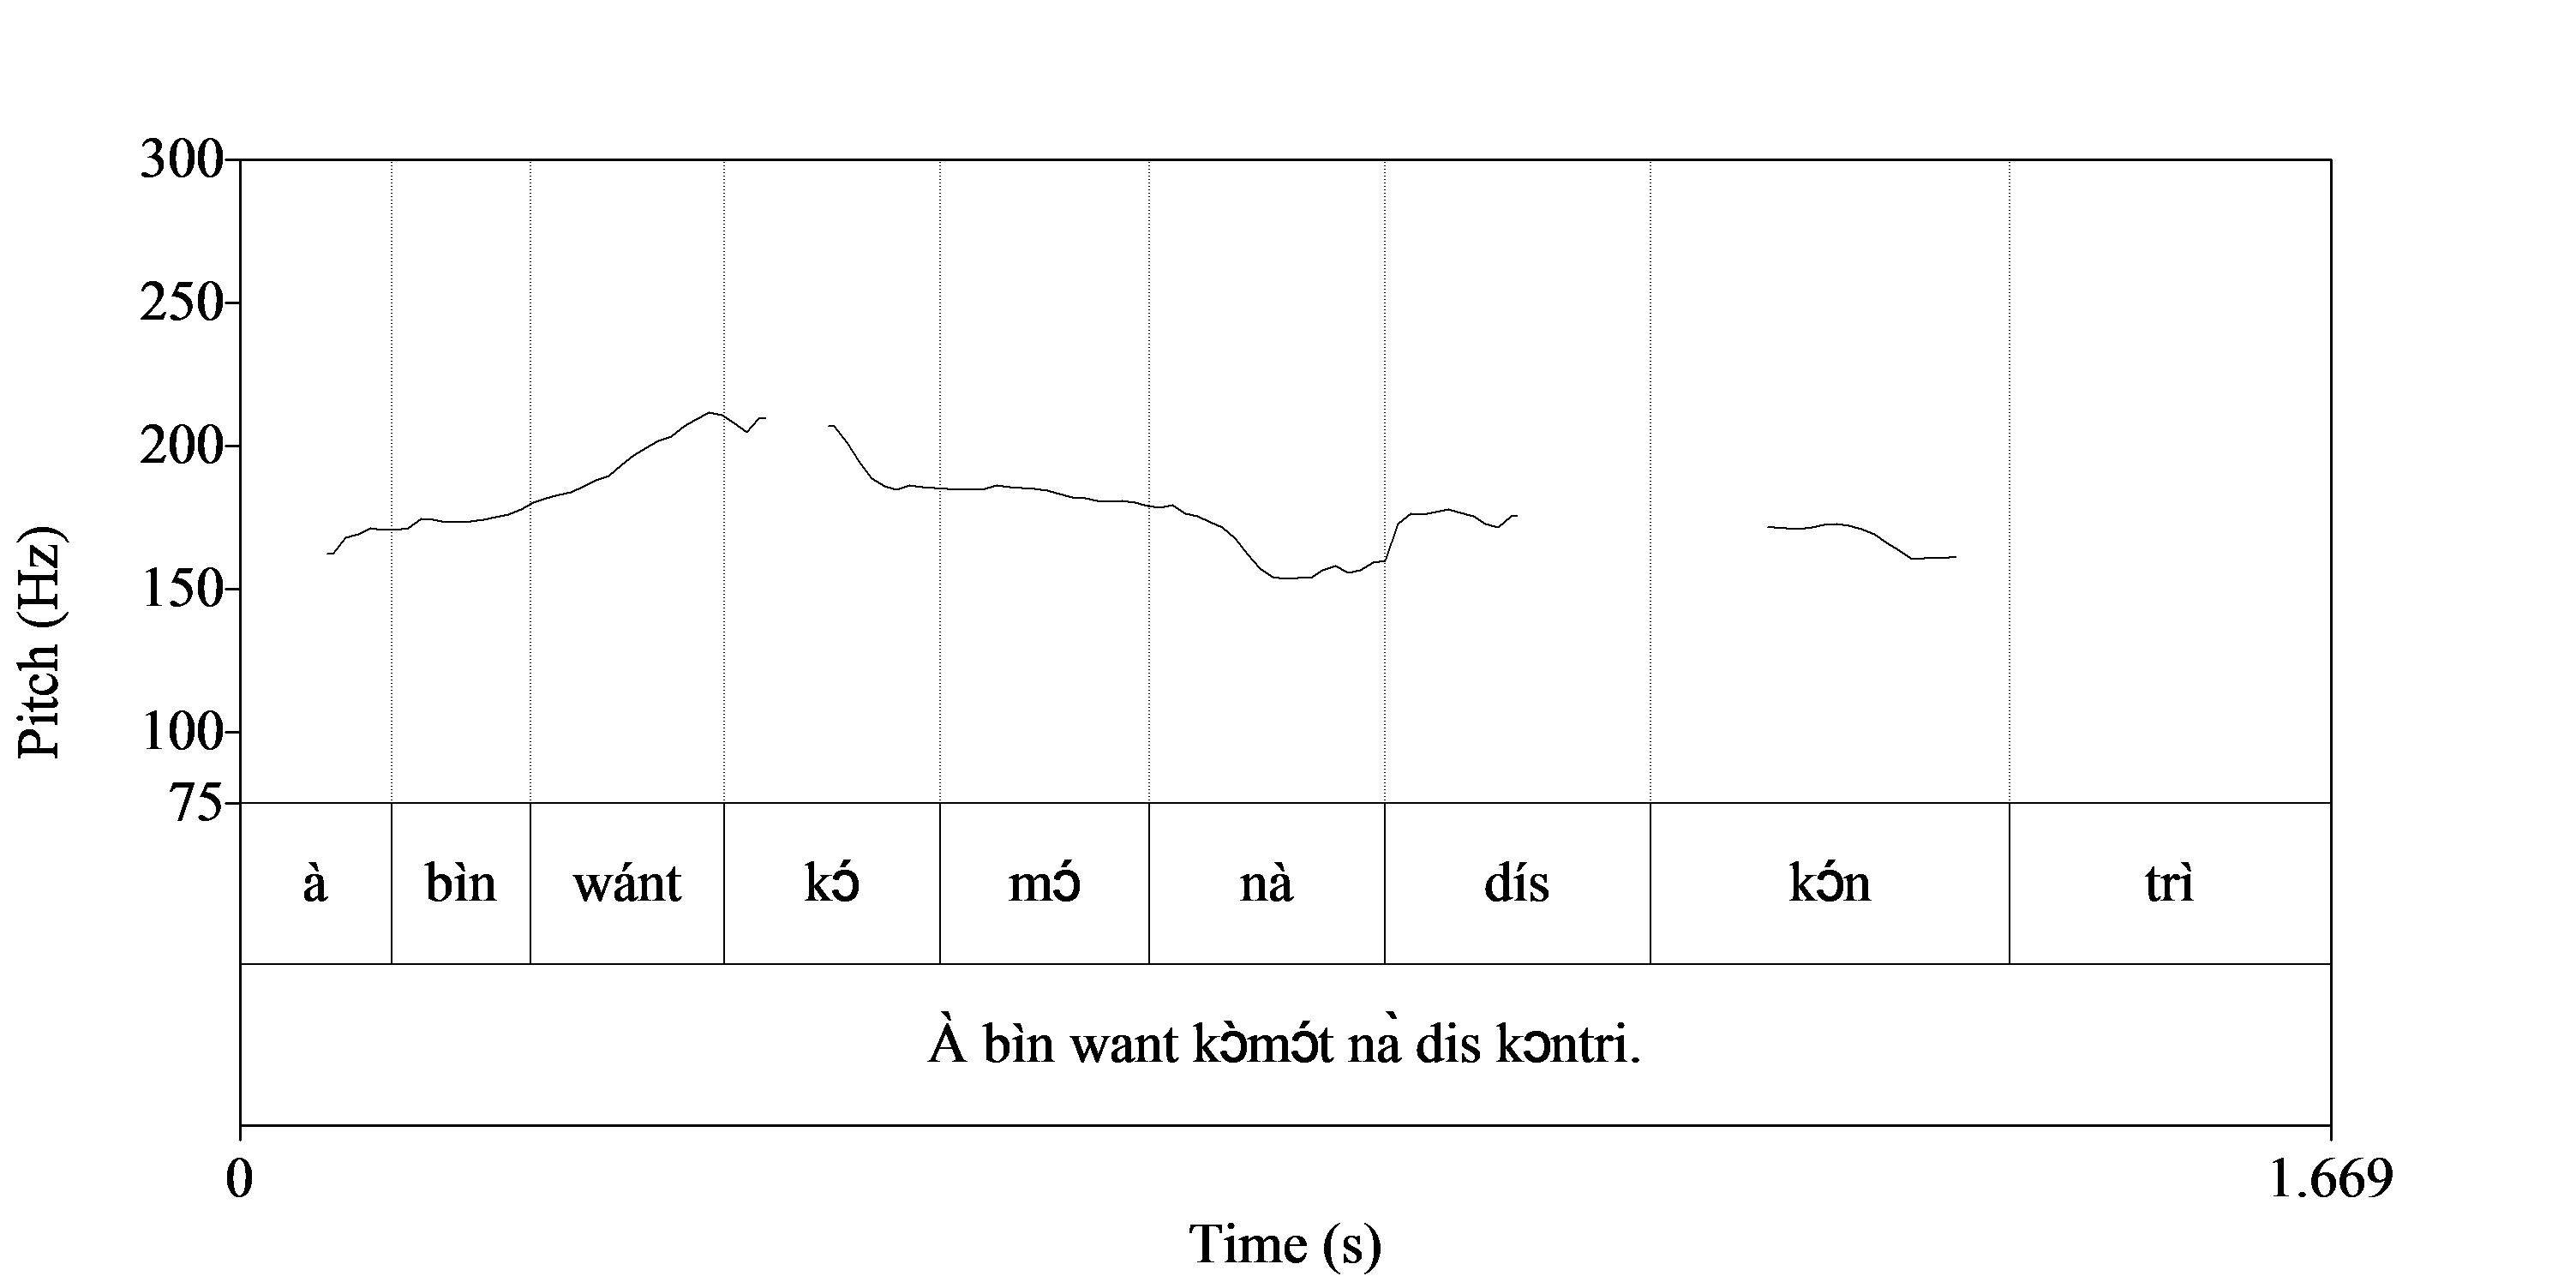
\includegraphics[height=.3\textheight]{figures/yakpomod-img29.png}
\end{figure}

%%[Warning: Draw object ignored]
 
\ea%80
    \label{ex:key:80}
    \glll   A    bin  wánt  kɔmɔ́t  na  dís  kɔ́ntri.\\
\textsc{l}    \textsc{l}  \textsc{h}    \textsc{l.h}    \textsc{l}  \textsc{h}  \textsc{h.l}\textbf{\textsc{l\%}}\\
\textsc{1sg.sbj}  \textsc{pst}  want  go.out  \textsc{loc}  this  country\\
\glt ‘I wanted to leave this country.’→  
\z

In contrast, polysyllabic vowel-final words with a final lexical H tone do not usually feature an utterance-final fall in non-emphatic declaratives. They retain their word-final H tone. Compare \textit{bɔbí} ‘breast’ in \figref{fig:key:3.28}: 

\begin{figure}
\caption{Unpronounced declarative L\% over L.H word}
\label{fig:key:3.28}
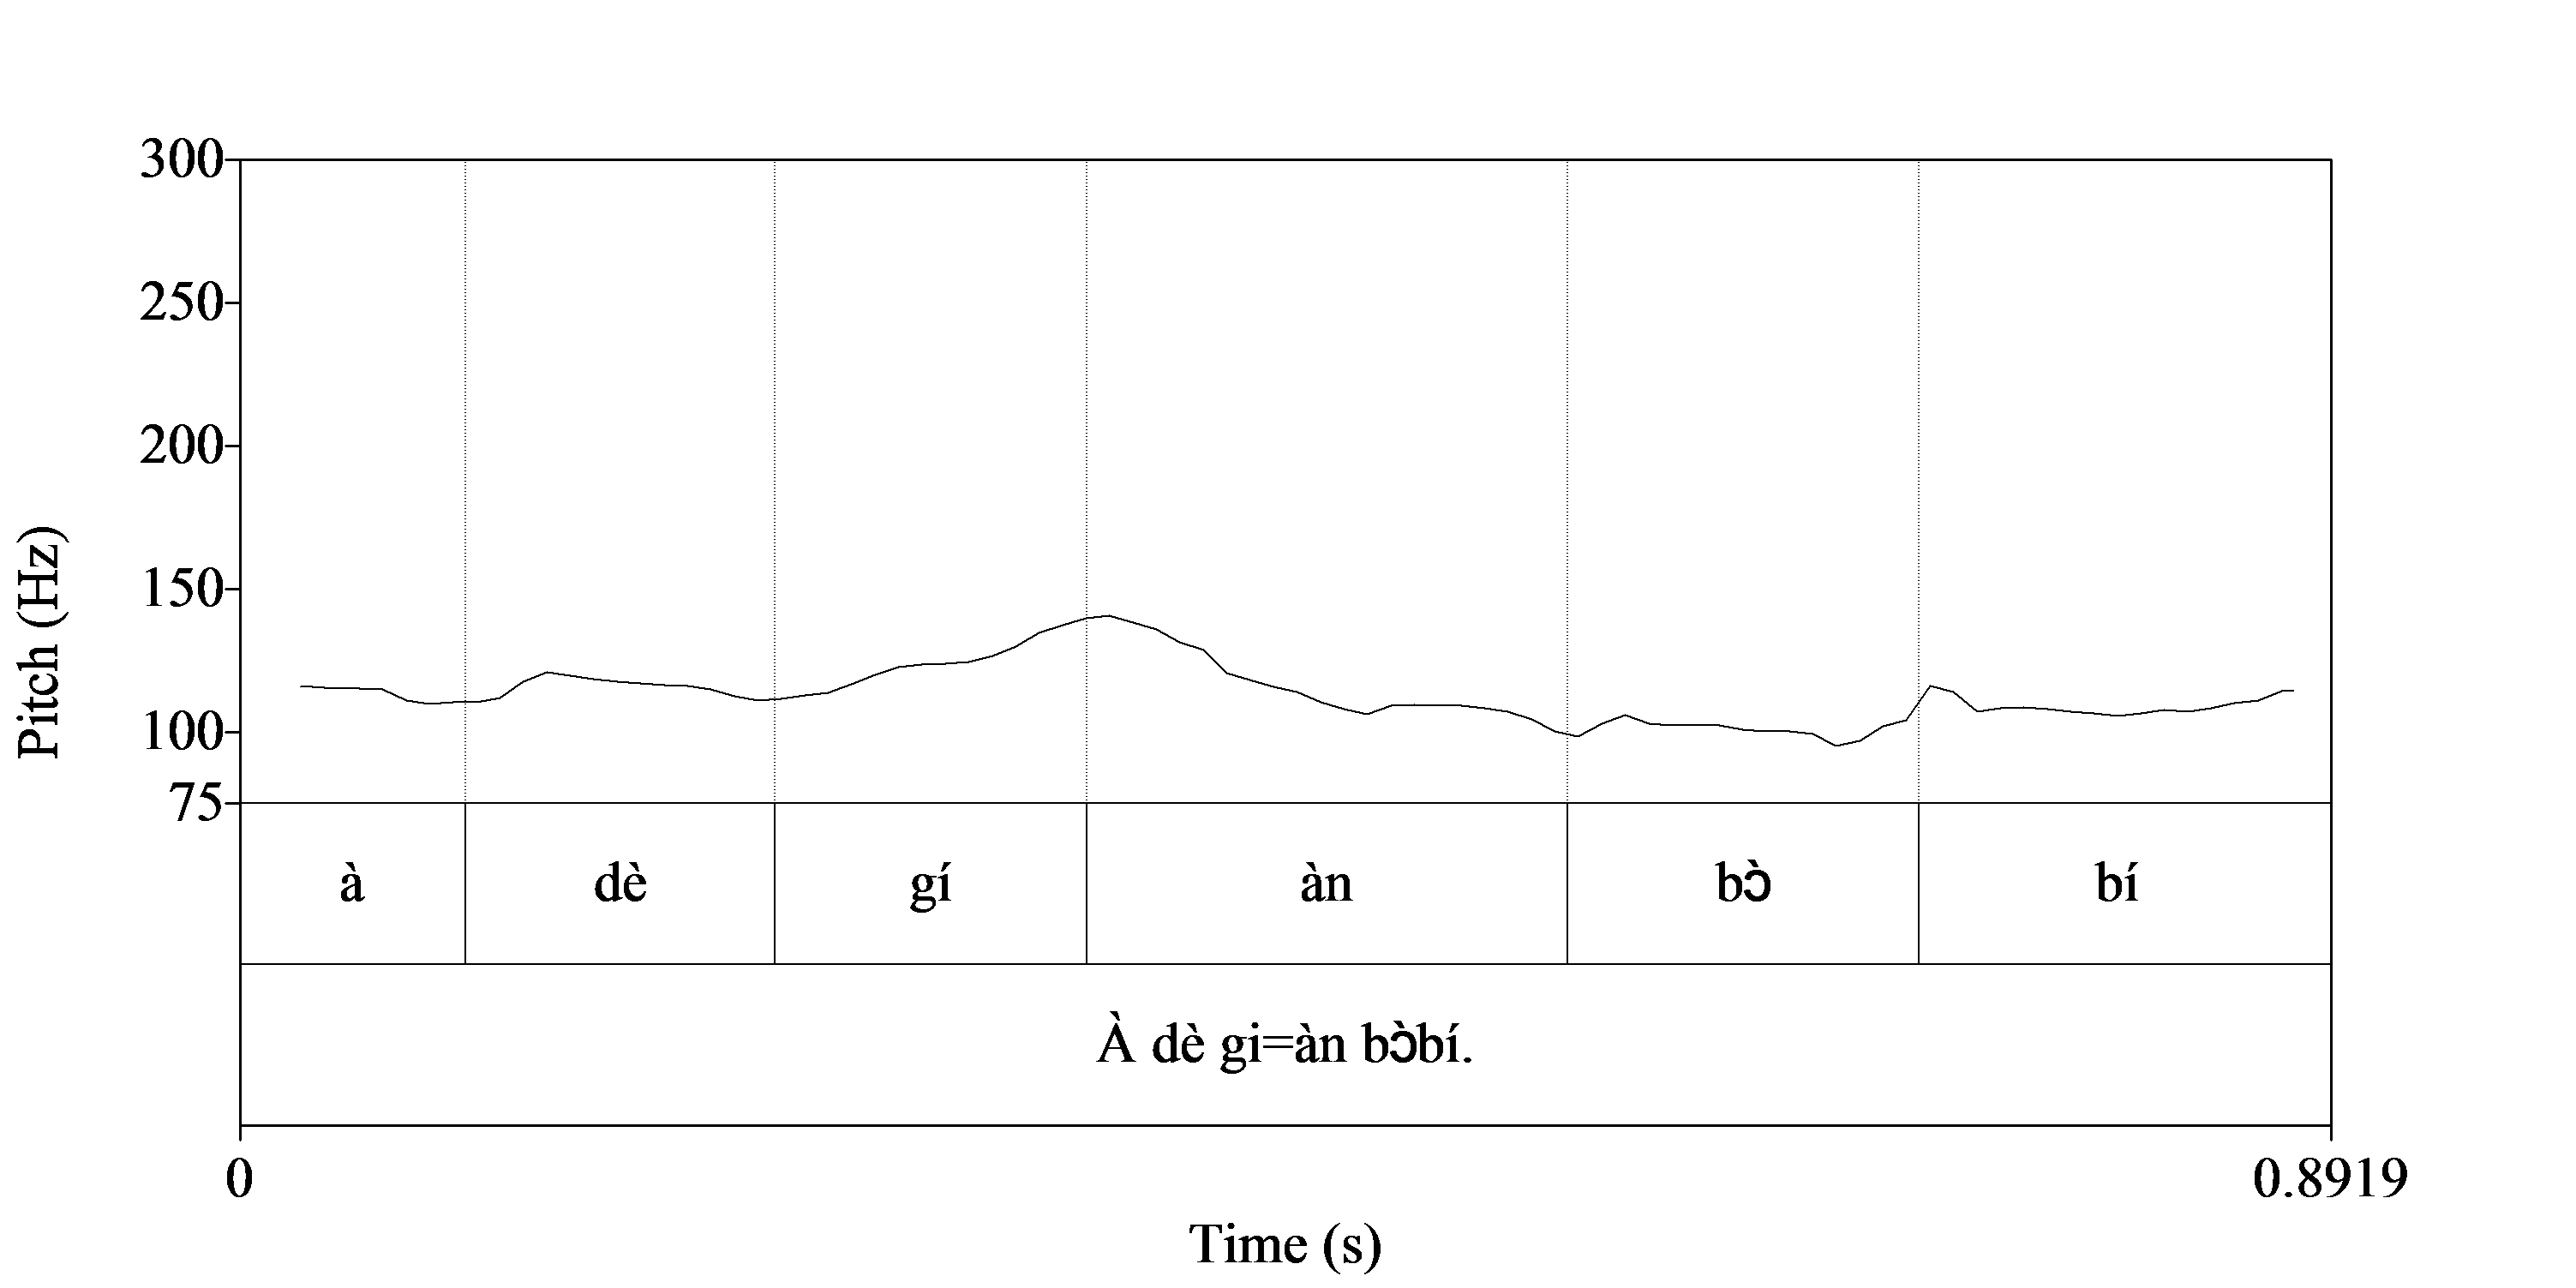
\includegraphics[height=.3\textheight]{figures/yakpomod-img30.png}
\end{figure}
 


\ea%81
    \label{ex:key:81}
    \gll   \MakeUppercase{A}   de    gí=an    bɔbí.\\
\textsc{l}    \textsc{l}    \textsc{h=l}      \textsc{l.}\textbf{\textsc{h}}\\


\textsc{1sg.sbj}  \textsc{ipfv}    give  =\textsc{3sg.obj}  breast\\

\glt ‘I’m breast-feeding her.’  

\z

Content questions\is{content questions} feature the same boundary tone as declaratives. Compare the utterance-final fall over the monosyllable in \figref{fig:key:3.29}:

\begin{figure}
\caption{L\% with content question}
\label{fig:key:3.29}
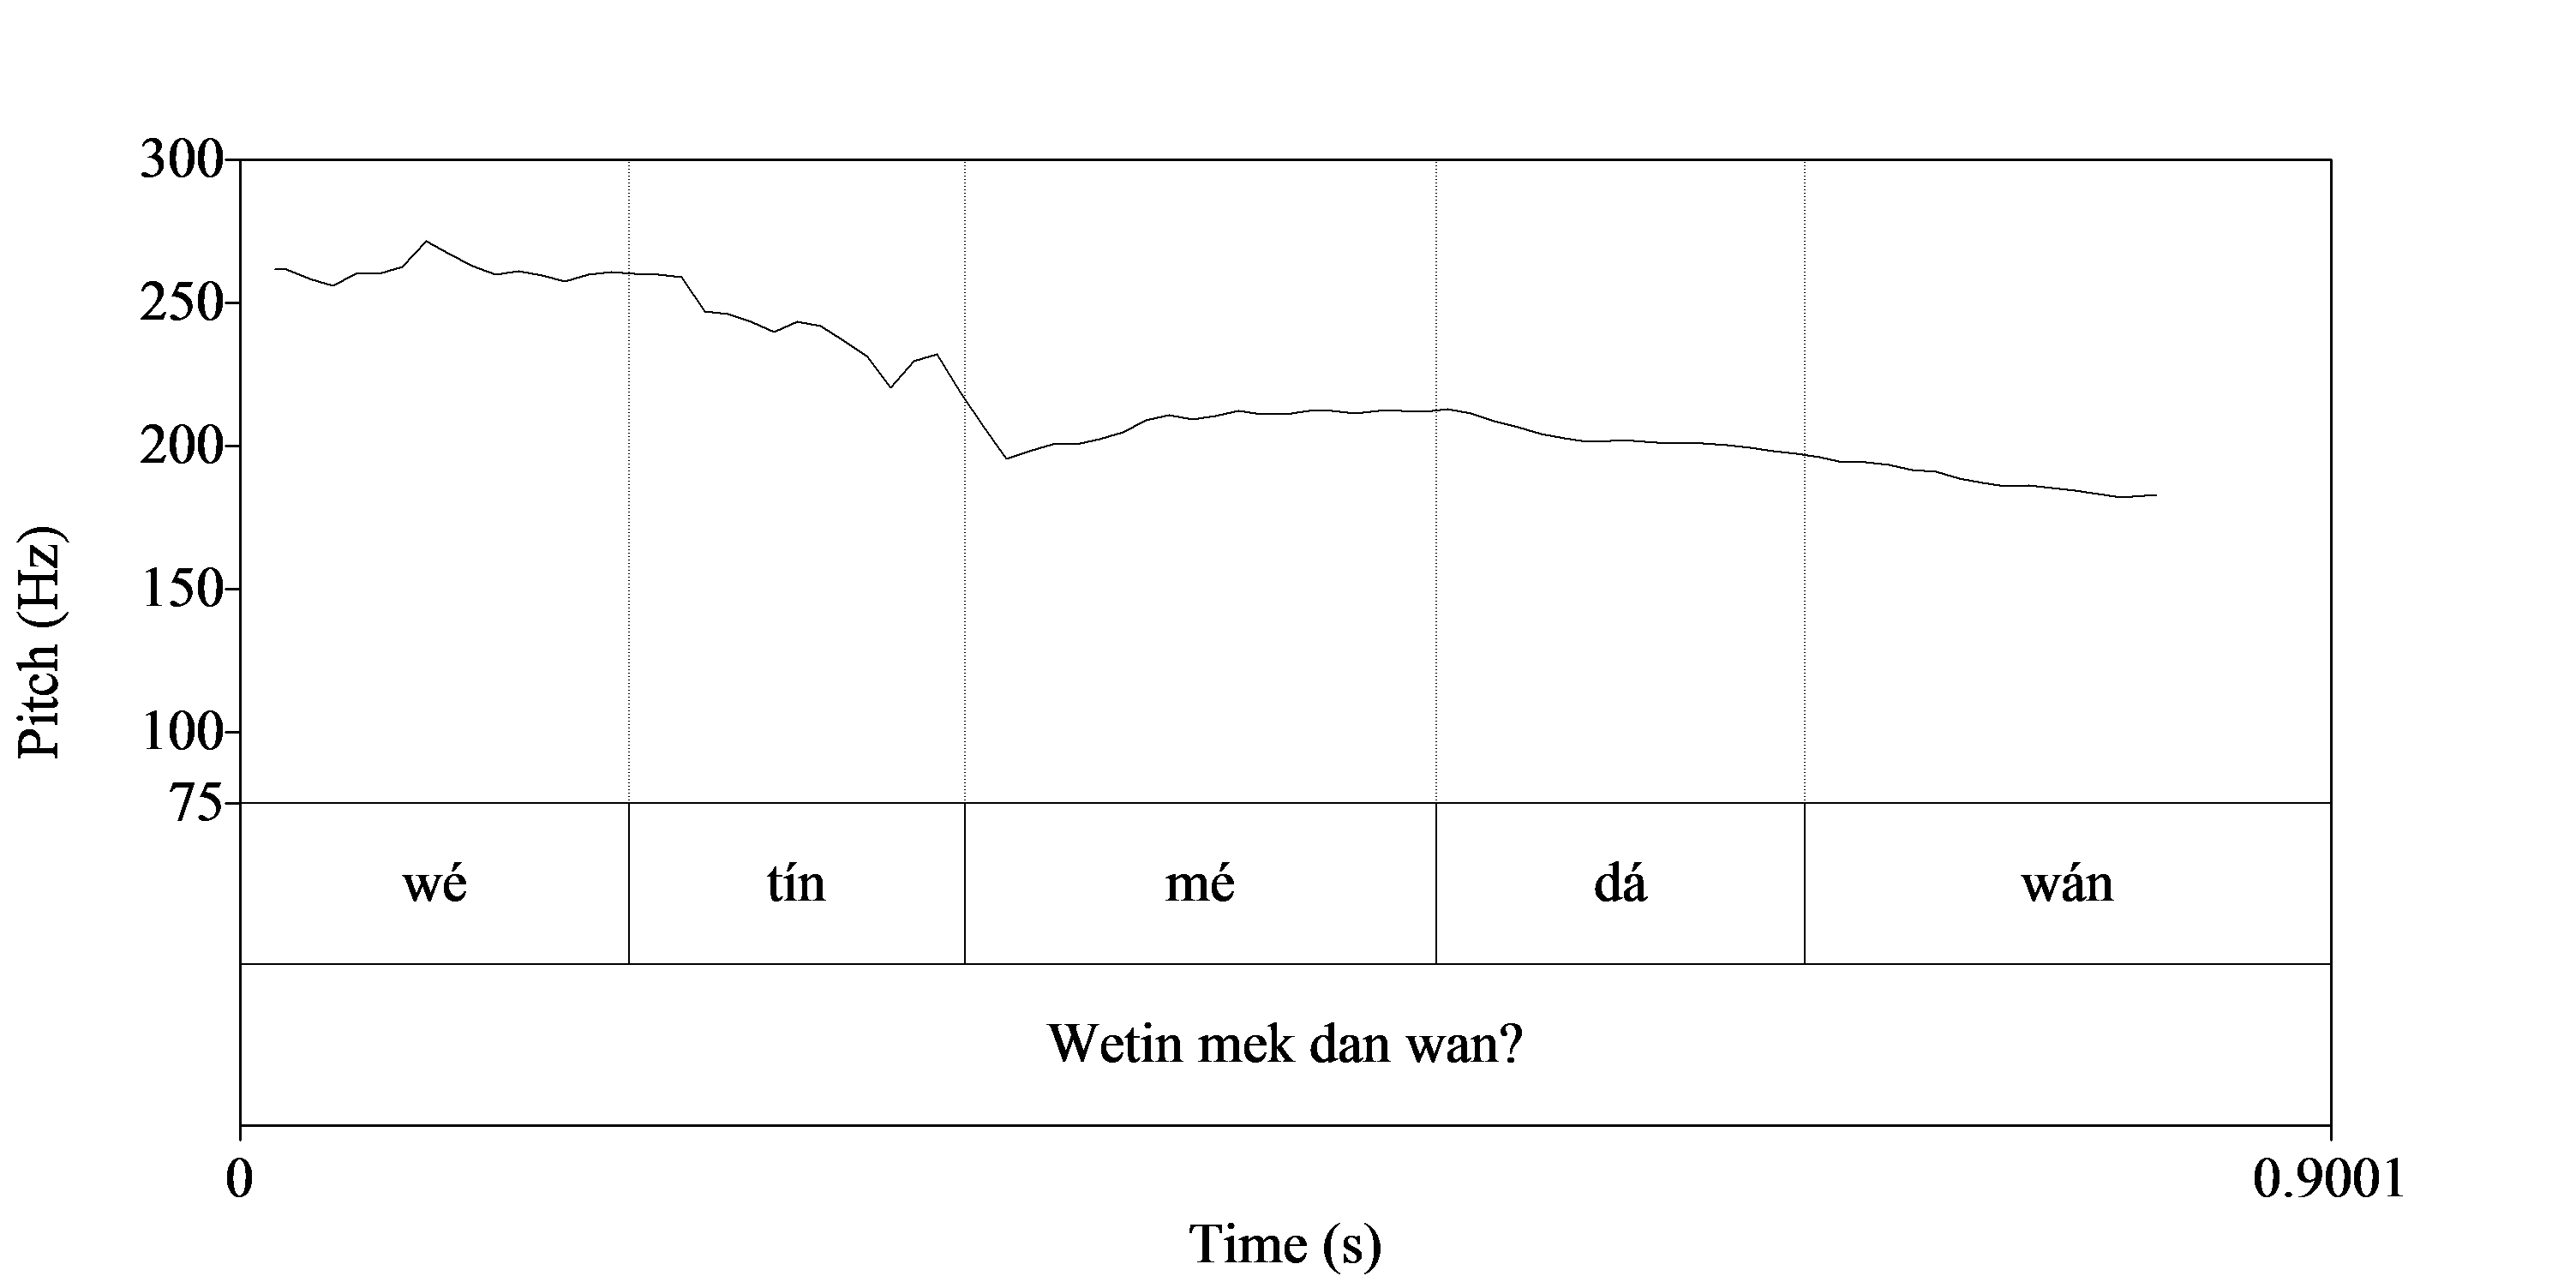
\includegraphics[height=.3\textheight]{figures/yakpomod-img31.png}
\end{figure}

  
 


\ea%82
    \label{ex:key:82}
    \gll   Wétin  mék    dán    \textbf{wán}?  \\
\textsc{h.l}    \textsc{h}    \textsc{h}    \textbf{\textsc{hl\%}}      \\
what  make  that    one\\
\glt ‘What causes this?’\is{declarative intonation}
\z

\subsection{Emphatic intonation}\label{sec:3.4.2}

Emphatic intonation expresses meanings like extra-emphasis, insistence, impatience or reproach. There are two ways of signalling emphasis\is{emphasis} at the sentence level in Pichi\is{emphatic stress}. One way involves the use of the emphatic LH\% boundary tone. A second way involves the use of pitch range expansion (cf. \sectref{sec:3.2.5}).


The emphatic LH\% is an additive contour tone. It succeeds the  lexical tone of the utterance-final syllable, which may therefore count up to three beats in length. Additionally, the last lexical H before the LH\% boundary contour tone is often pronounced with an extra-high tone due to emphasis. This peculiar combination of an extra-high lexical tone and a contour boundary tone creates a highly perceptible utterance-final tonal melody. 



Phonemically, an utterance-final L to which the emphatic LH\% boundary tone associates bears an LHH sequence of tones. Phonetically, the utterance-final syllable is realised as an LH contour. \figref{fig:key:3.30} depicts the utterance-final rise over the L-toned monosyllable \textit{=an} ‘\textsc{3sg.obj’}. 


\begin{figure}
\caption{Emphatic LH\% over L-final word}
\label{fig:key:3.30}
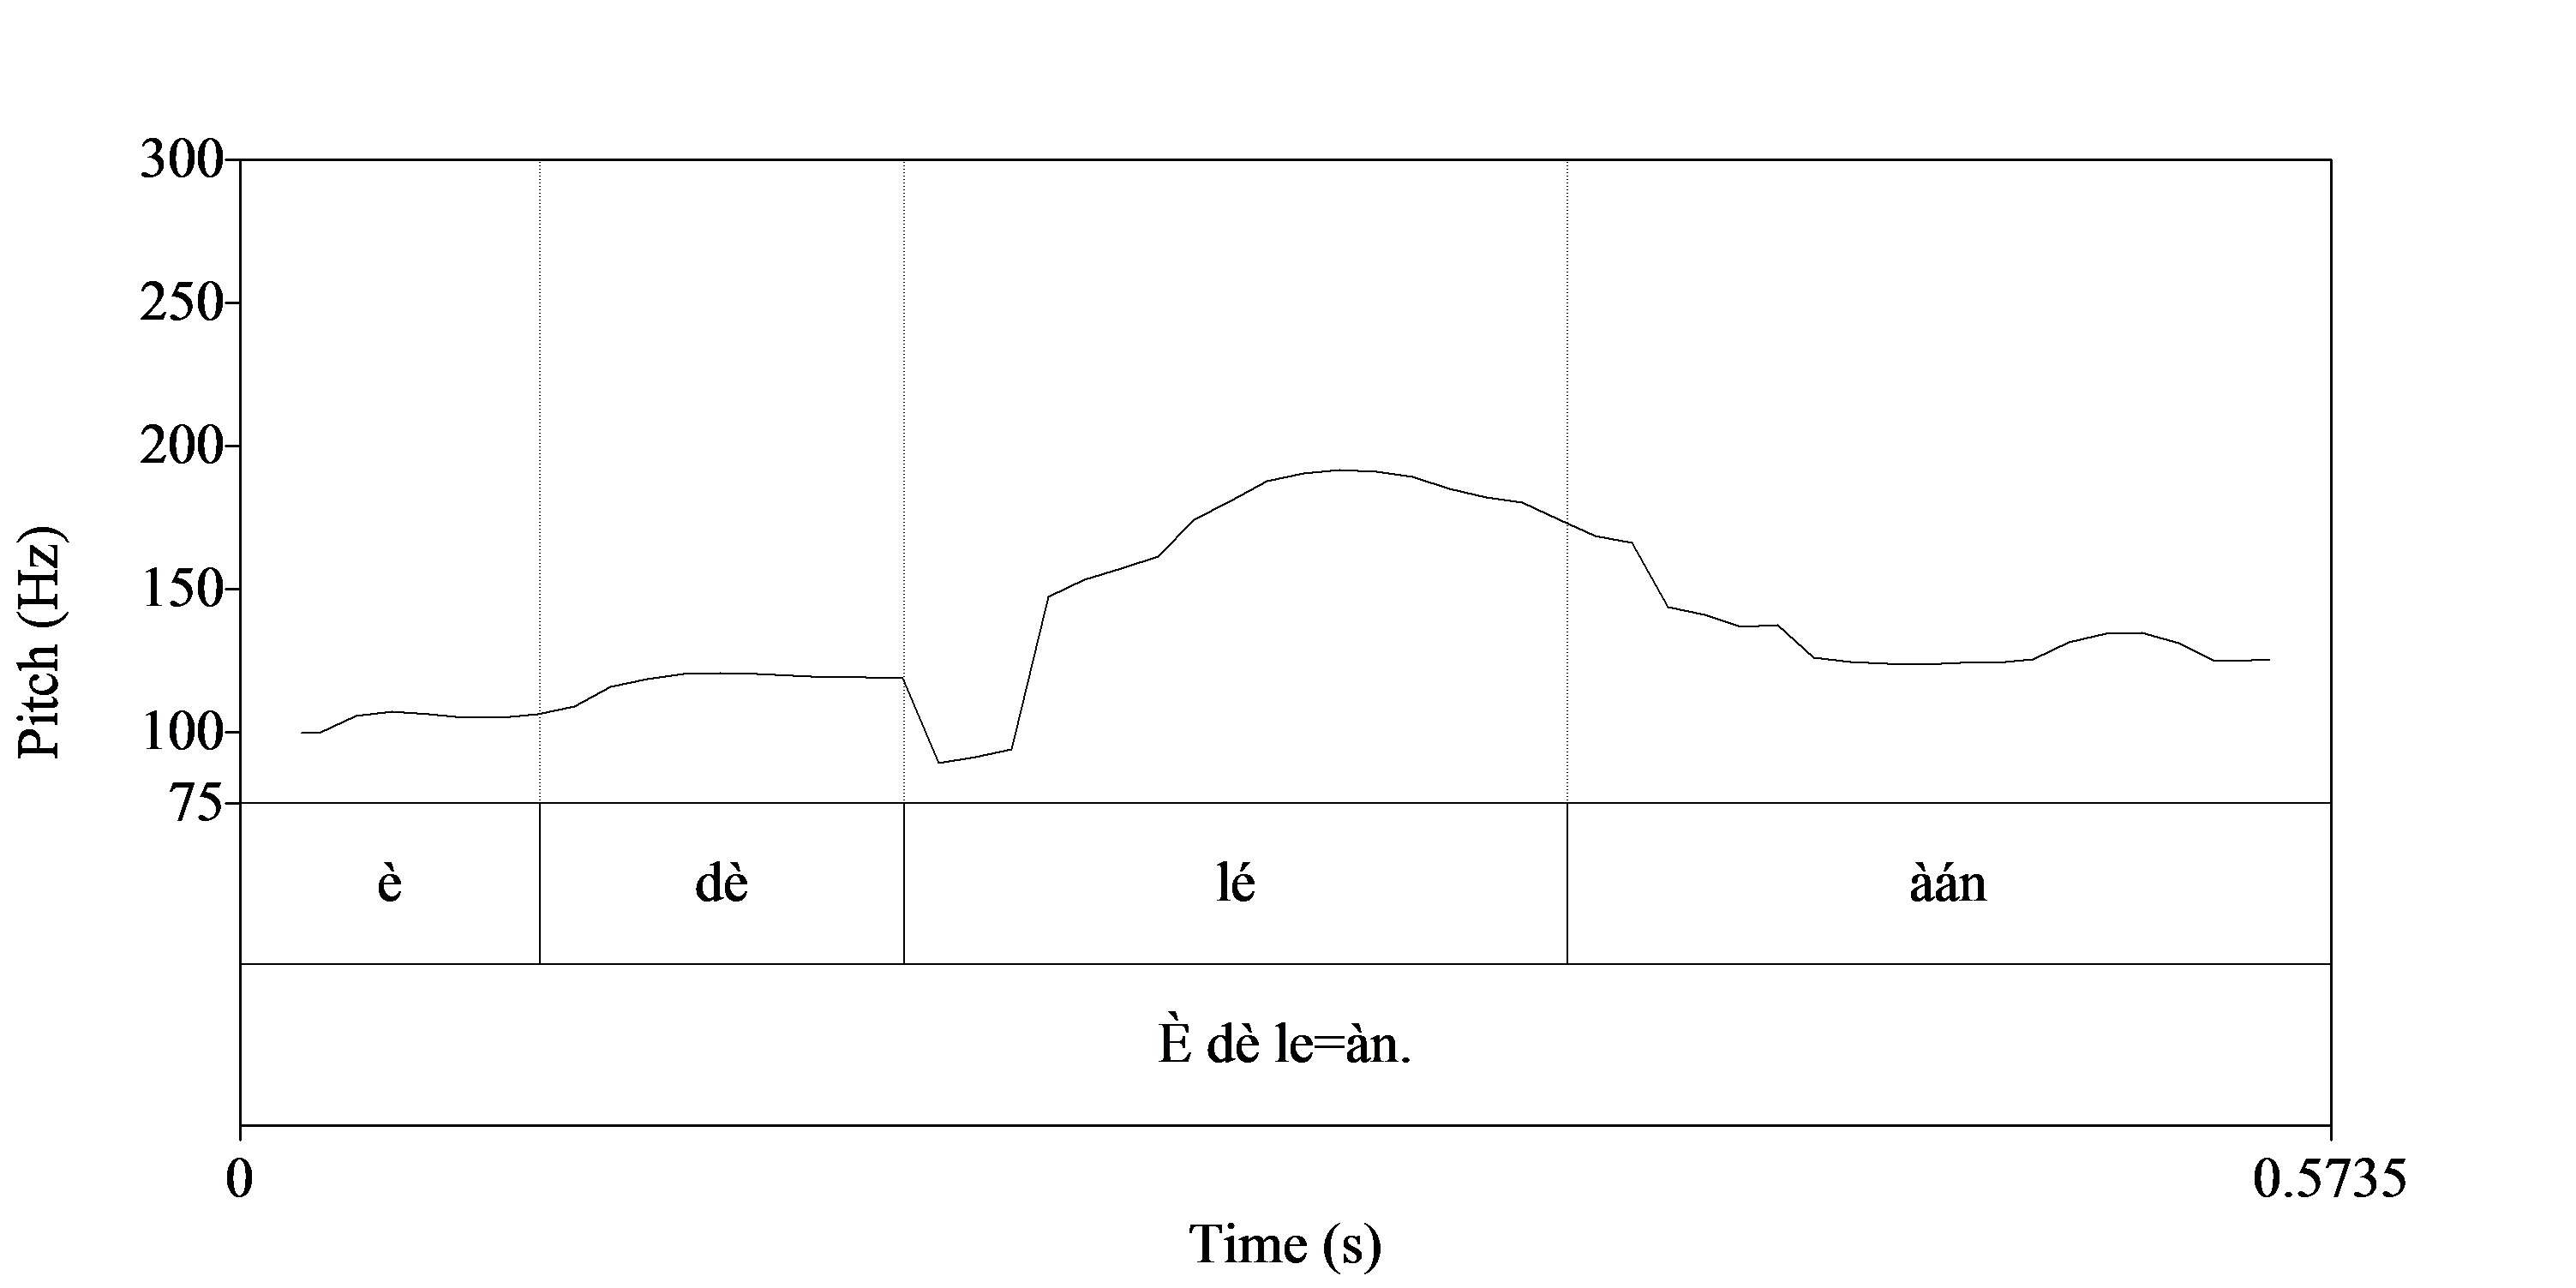
\includegraphics[height=.3\textheight]{figures/yakpomod-img32.png}
\end{figure}

  
 


\ea%83
    \label{ex:key:83}
    \gll   E    de  lé=an.\\
\textsc{l}    \textsc{l}  \textsc{h=}\textbf{\textsc{lh\%}}\\
\textsc{3sg.sbj}  \textsc{ipfv}    lay=\textsc{3sg.obj}\\
\glt ‘She is laying it (on the table).’
\z

When the emphatic boundary tone links with an utterance-final H-toned syllable the resulting contour features an initial rise, an intermediate fall, and a final rise. The utterance-final, extensively lengthened syllable thus bears an HLH contour. Compare the utterance-final H-toned monosyllables \textit{ín} ‘\textsc{3sg.indp}’ and \textit{gó} ‘go’ in the following two tables: 

% TODO: put in quadrant

\begin{figure}
\caption{Emphatic LH\% over H-final word}
\label{fig:key:3.31}
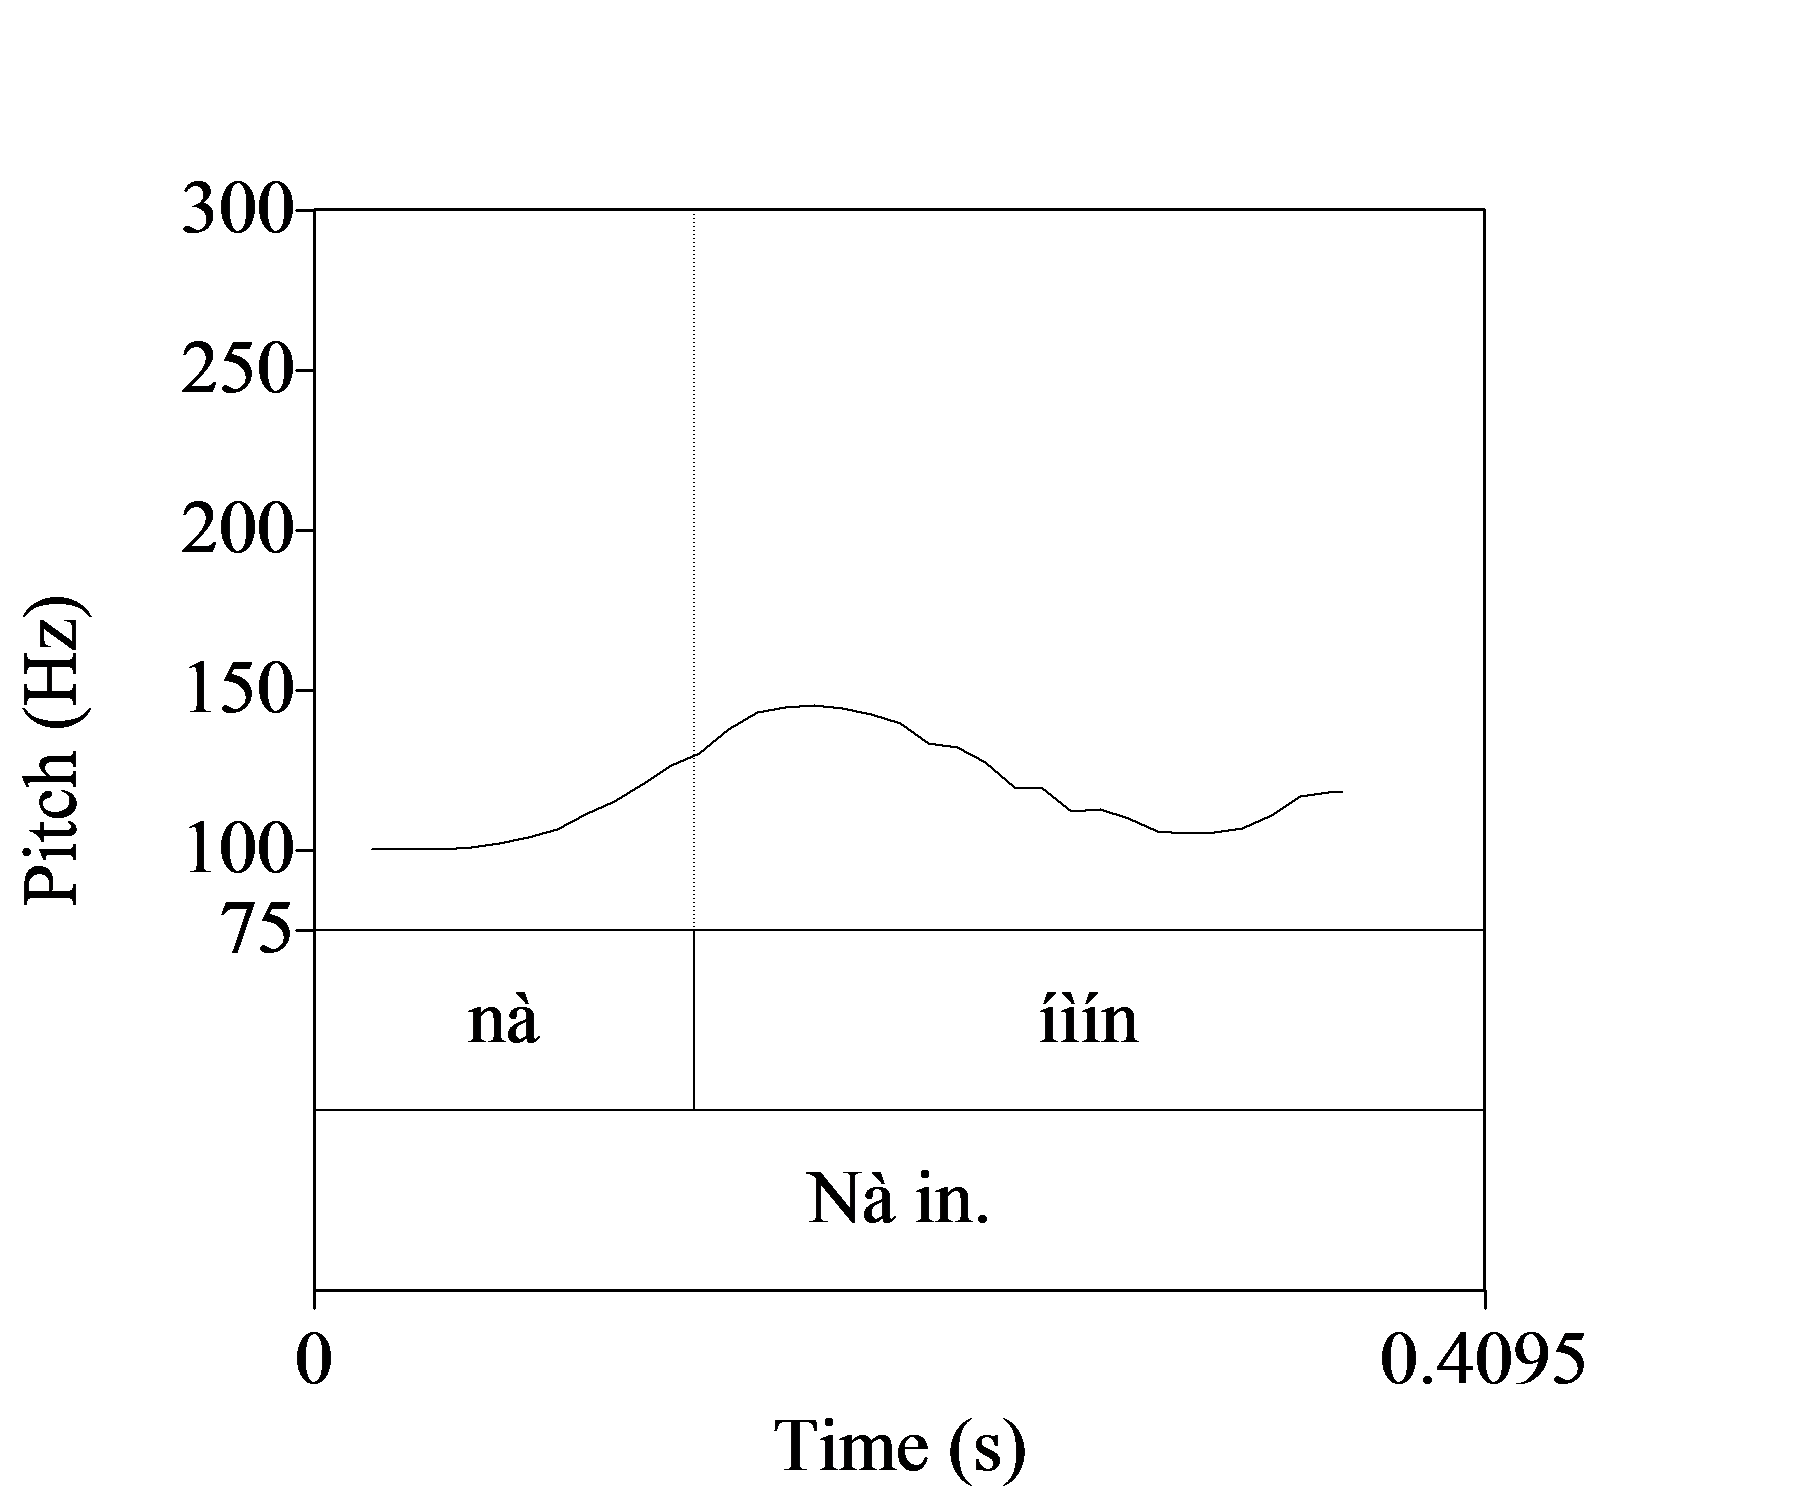
\includegraphics[height=.3\textheight]{figures/yakpomod-img33.png}
\end{figure}

\begin{figure}
\caption{Emphatic LH\% over H-final word}
\label{fig:key:3.32}
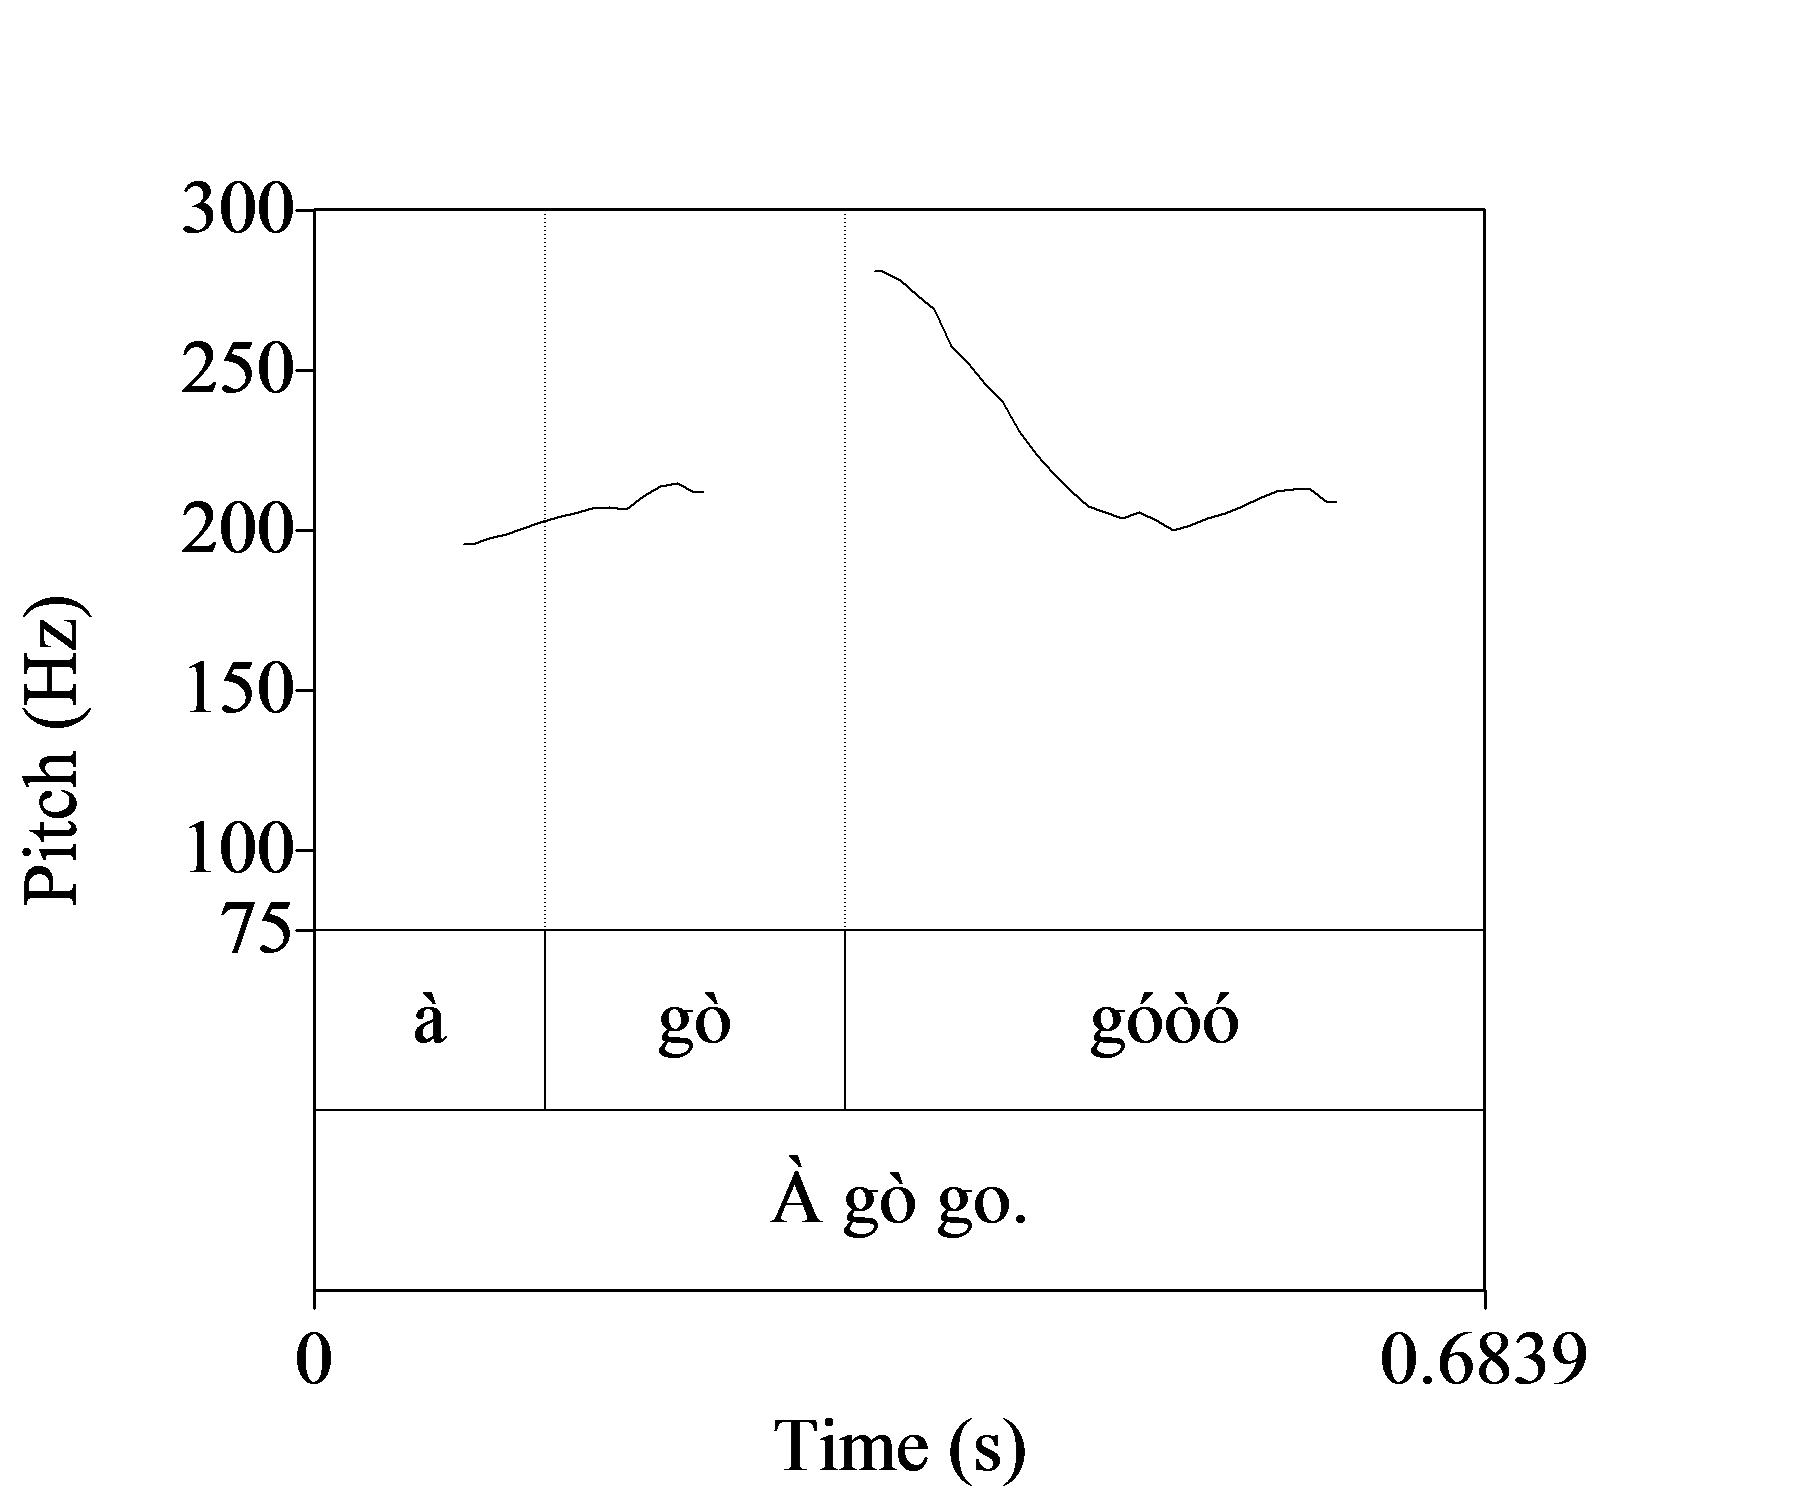
\includegraphics[height=.3\textheight]{figures/yakpomod-img34.png}
\end{figure}  

\ea\label{ex:key:84}
\glll Na  \textstylePichiexamplebold{ín}.''\\
\textsc{l}  \textbf{\textsc{h}}\textstylePichiexamplebold{\textsc{lh\%}}\\
\textsc{foc}  \textsc{3sg.indp}\\
\glt   ‘That’s it [you should know that].’
\z
\ea\label{ex:key:85}
\glll    A    go  \textbf{gó}.  \\
\textsc{l}    \textsc{l}  \textbf{\textsc{h}}\textstylePichiexamplebold{\textsc{lh\%}}\\
\textsc{1sg.sbj}  \textsc{pot}  go\\
\glt   ‘I’ll go [you don’t need to remind me to].’ 
\z

An utterance-final, H-toned syllable of a polysyllabic word also bears this contour. Compare \textit{bɔbí} ‘breast’ and \textit{chukchúk} ‘thorn’ in the following tables. The two words were pronounced with emphatic intonation during vocabulary elicitation because the speaker expected me to be familiar with them: 

\begin{figure}
\caption{H\% over vowel-final L.H word}
\label{fig:key:3.33}
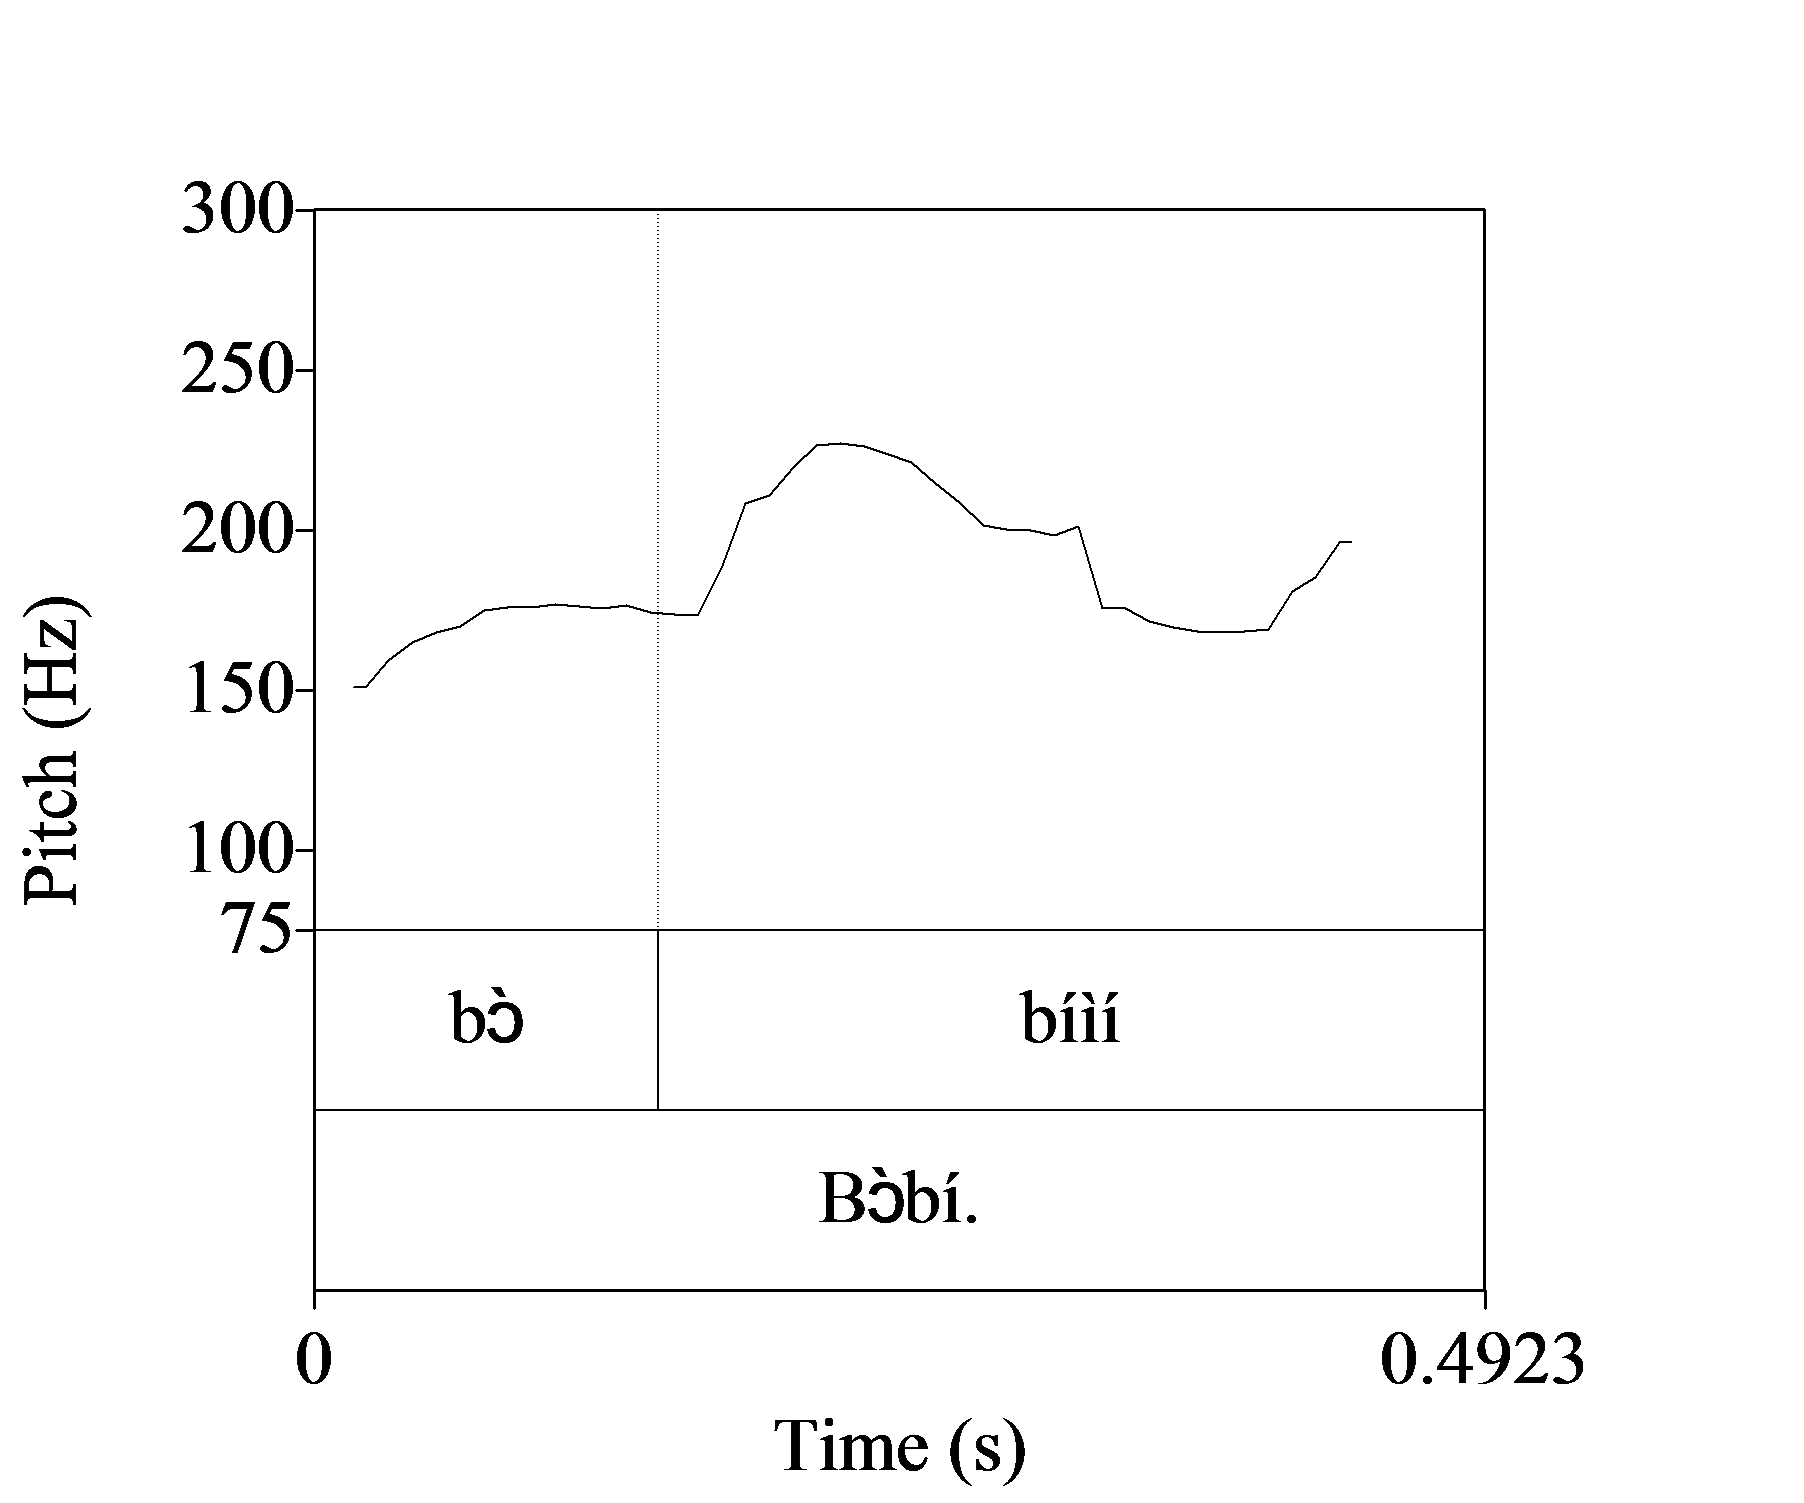
\includegraphics[height=.3\textheight]{figures/yakpomod-img35.png}
\end{figure}


\begin{figure}
\caption{H\% over obstruent-final L.H word}
\label{fig:key:3.34}
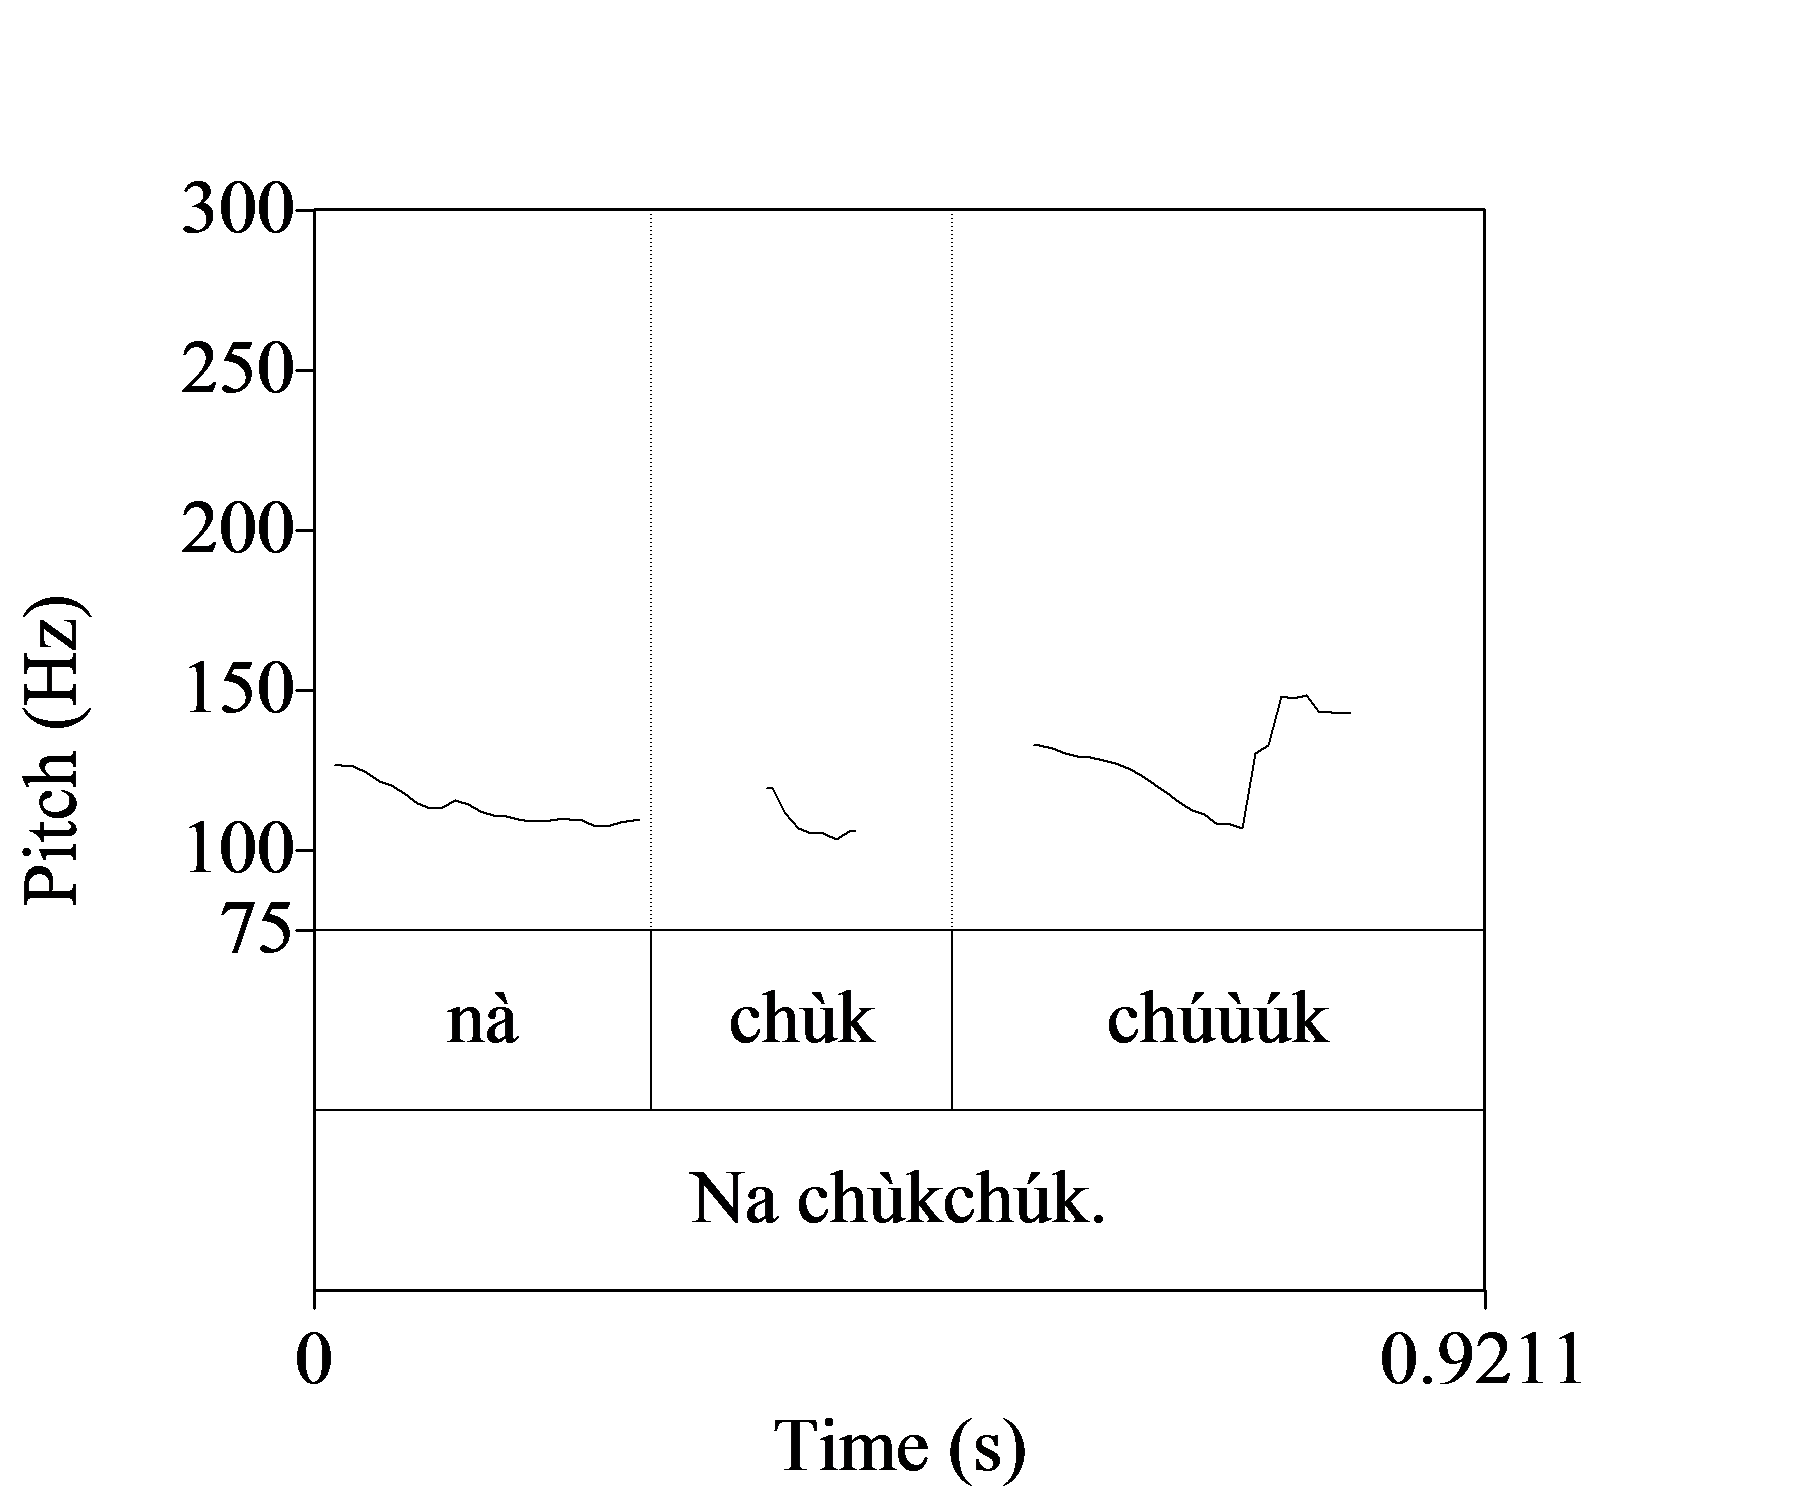
\includegraphics[height=.3\textheight]{figures/yakpomod-img36.png}
\end{figure}

\ea%86
    \label{ex:key:86}
    \glll   Bɔbí.\\
\textsc{l.}\textbf{\textsc{h}}\textstylePichiexamplebold{\textsc{lh\%}}\\
breast\\
\glt ‘Breast [that’s self-evident!].’ 
\z

\ea
\label{ex:key:87}
\glll \textstylePichiexamplenumberZchnZchn{Na  chukchúk}\\
\textsc{l}  \textsc{l.}\textbf{\textsc{hlh\%}}\\
\textsc{foc}  thorn\\
\glt ‘It’s a thorn [that’s self-evident].’\is{emphatic intonation}
\z
The LH\% boundary contour tone is a loan\is{loan intonation} from (Equatoguinean and, ultimately, Iberian) Spanish together with the meanings associated with it. The LH\% contour boundary tone is also employed for list intonation \is{list intonation}(cf. \sectref{sec:3.4.3}). The following table presents the pitch trace of an utterance in Equatoguinean Spanish.


Compare the contour over the utterance-final L-toned syllable with that borne by the utterance-final L-toned syllable in \figref{fig:key:3.30} further below. Also compare the emphatic contour over the phonologically independent \textit{sí} ‘yes’ with that of the high-toned \textit{ín} ‘\textsc{3sg.indp}’ in \figref{fig:key:3.31}:


\begin{figure}
\caption{Emphatic intonation in peninsular Spanish}
\label{fig:key:3.35}
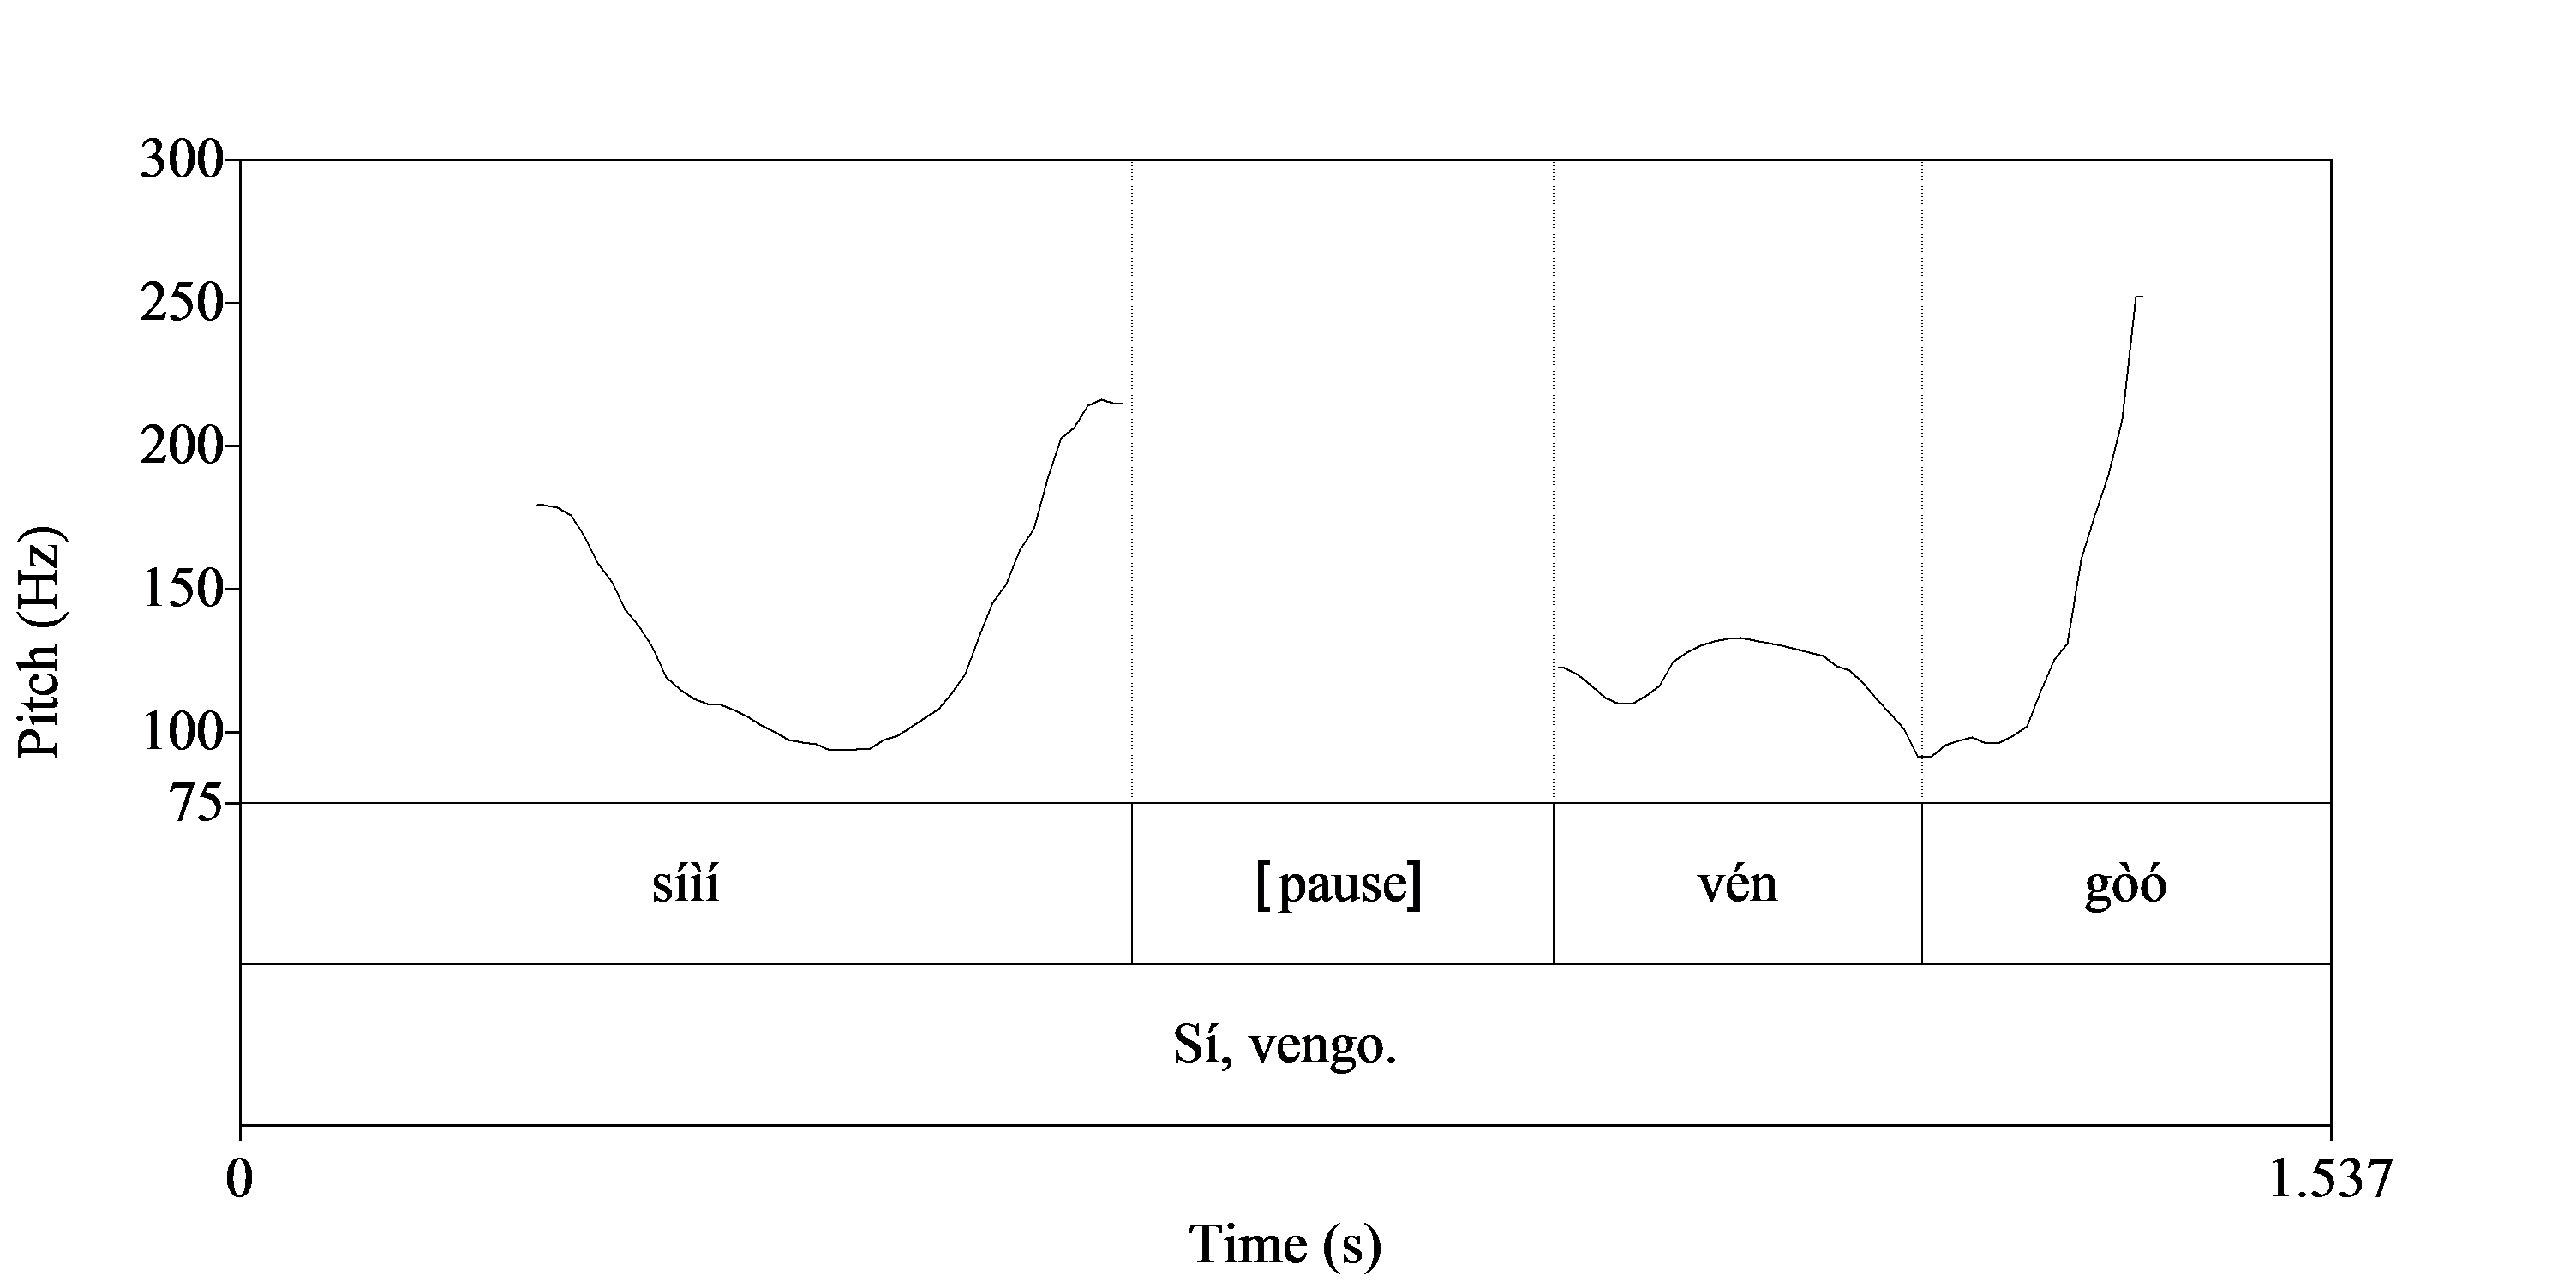
\includegraphics[height=.3\textheight]{figures/yakpomod-img37.png}
\end{figure}
 


\ea%88
    \label{ex:key:88}
    \glll   Sí    vengo.\\
\textsc{h}\textstylePichiexamplebold{\textsc{lh\%}}  \textsc{h.}\textstylePichiexamplebold{\textsc{lh\%}}\\
yes    I.come\\
\glt ‘Yes [you should know that!], I’ll come.’
\z

\subsection{List intonation}\label{sec:3.4.3}

The additive LH\% boundary tone employed for emphatic intonation is also used for list intonation. As in emphatic declaratives, LH\% associates with the final syllable and creates an LH contour over an utterance-final L-toned syllable and an HLH contour over an utterance-final H-toned syllable. The same intonation contour is once more found in Equatoguinean (and Iberian) Spanish with a similar range of meanings.


The following three pitch traces form part of a list. Take note of the LH contour over the L-toned dependent pronoun \textit{dɛn} ‘\textsc{3pl}’ before the short pause, as well as the LH contour borne by the L-toned final syllable of \textit{manicura} ‘manicure’ in \figref{fig:key:3.36} and \textit{chía} ‘chair’ in \figref{fig:key:3.36}. Compare this with the declarative L\% over \textit{dé} ‘there’, the closing sentence of the list in \figref{fig:key:3.38}: 


\begin{figure}
\caption{List intonation}
\label{fig:key:3.36}
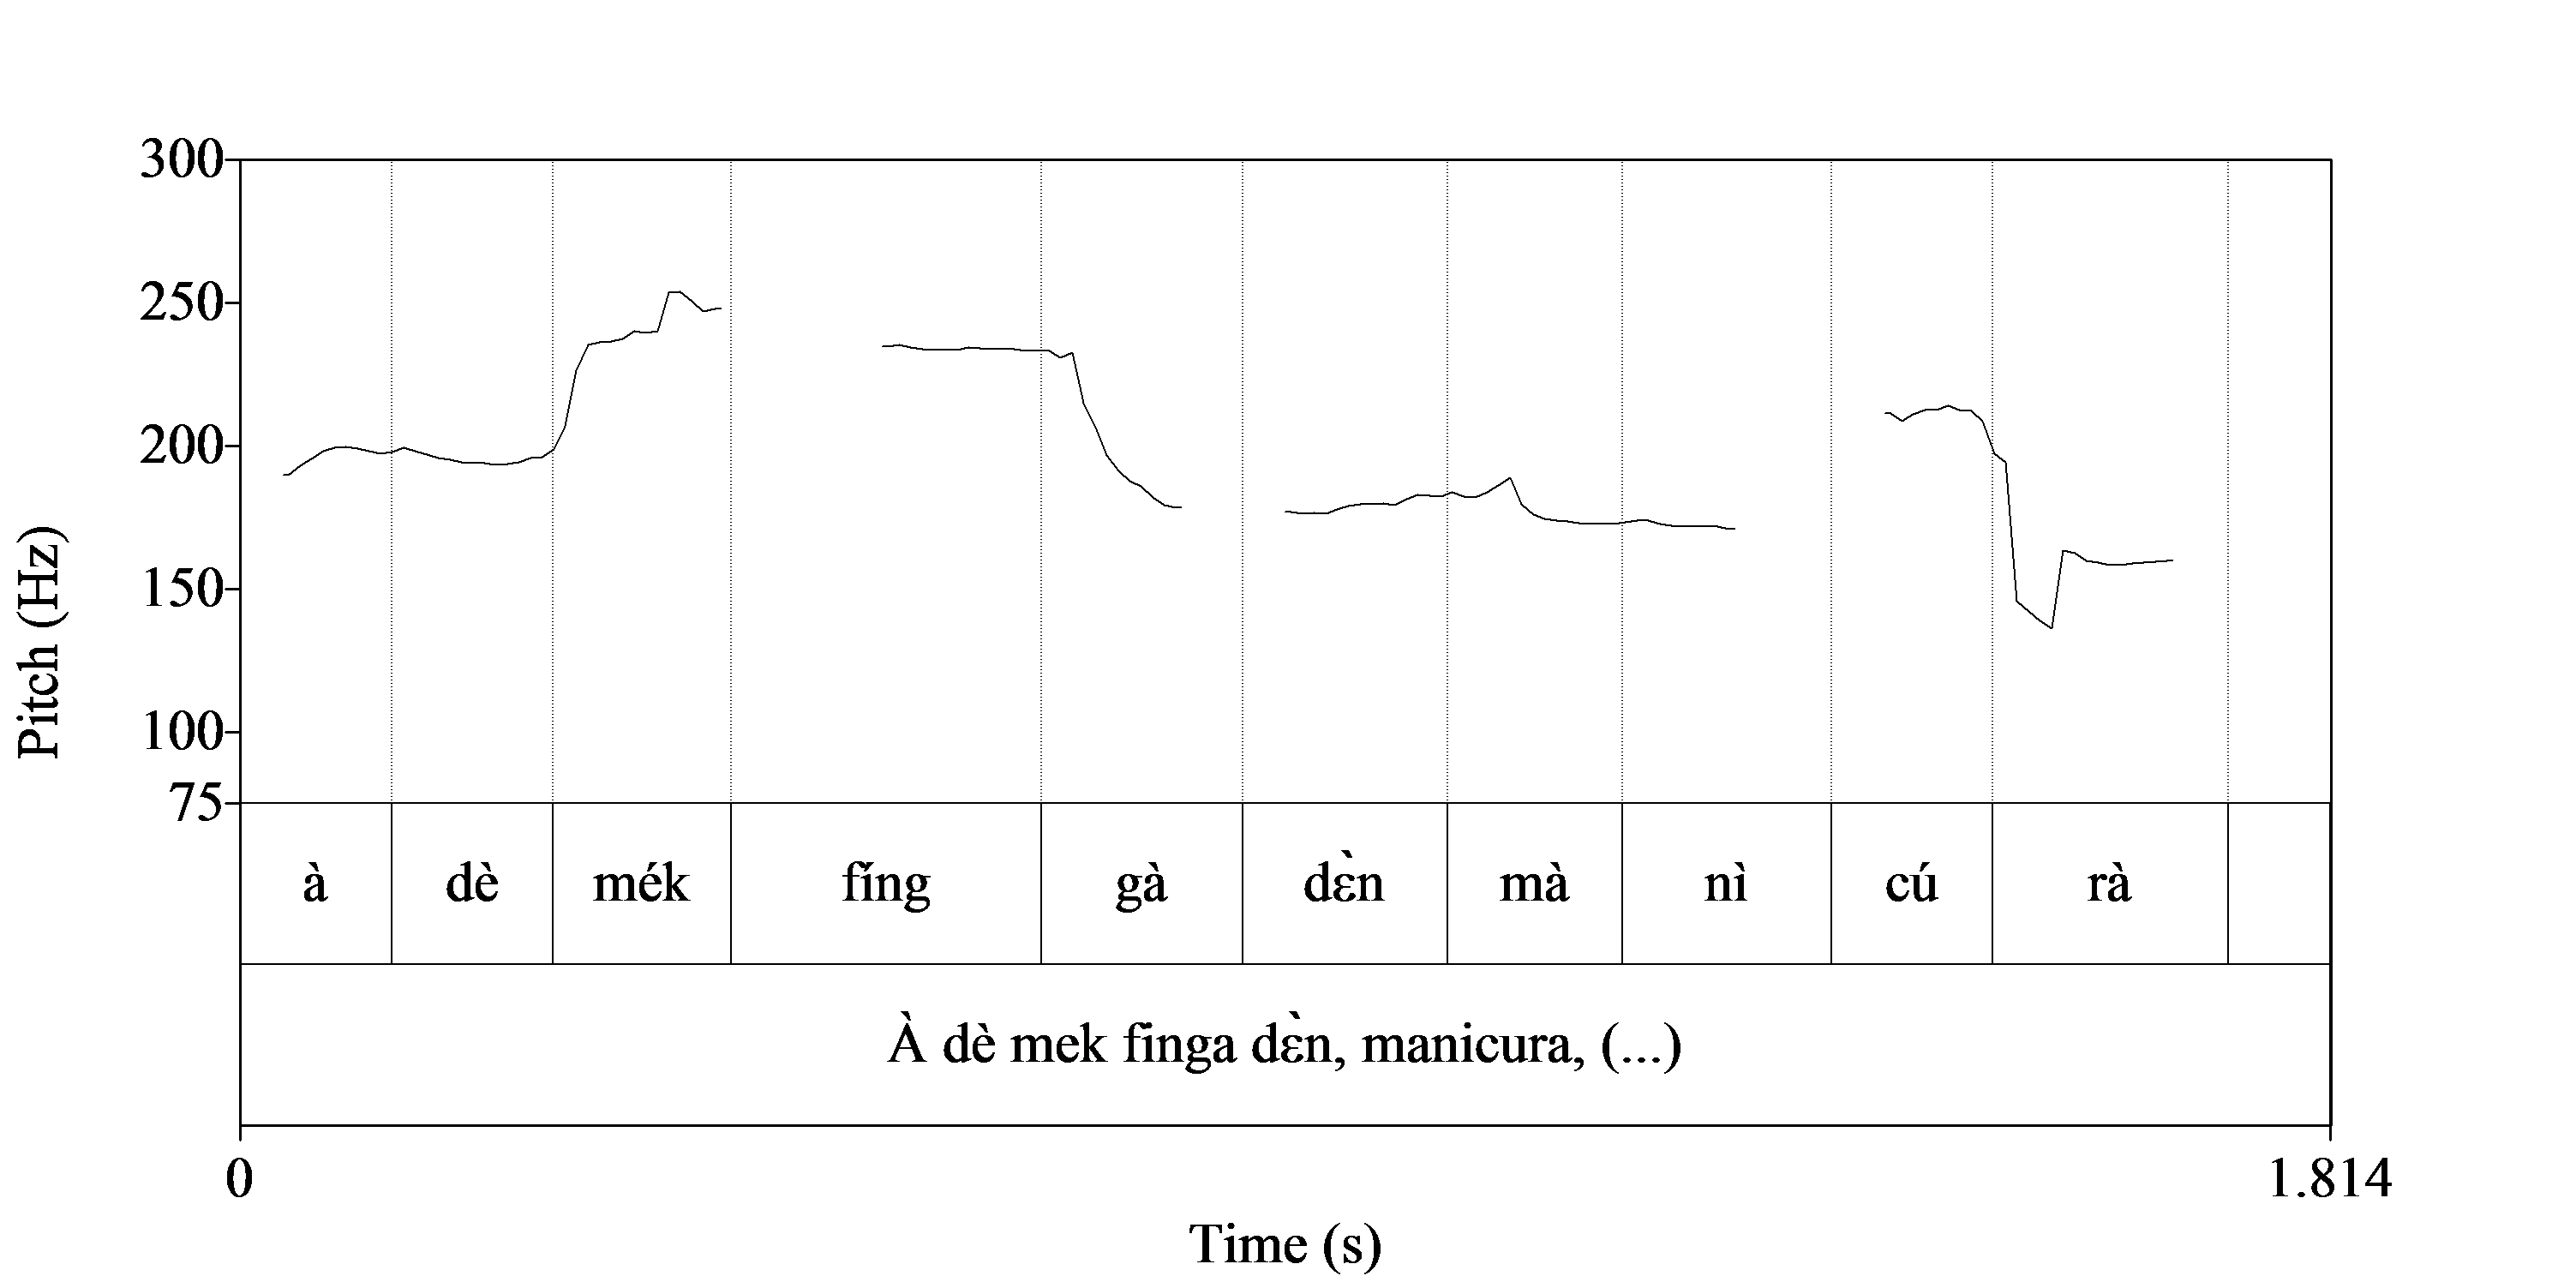
\includegraphics[height=.3\textheight]{figures/yakpomod-img38.png}
\end{figure}

  
 


\ea%89
    \label{ex:key:89}
    \glll   A    de  mék    fínga  \textstylePichiexamplebold{dɛn},    manicu\textbf{ra},  (...)\\
\textsc{l}    \textsc{l}  \textsc{h}    \textsc{h.l}    \textbf{\textsc{lh\%}}    \textsc{l.l.}\textbf{\textsc{h.lh\%}}\\
\textsc{1sg.sbj}  \textsc{ipfv}  make  finger  \textsc{pl}    manicure\\
\glt ‘I was making fingers, manicure (...)’
\z

\begin{figure}
\caption{List intonation}
\label{fig:key:3.37}
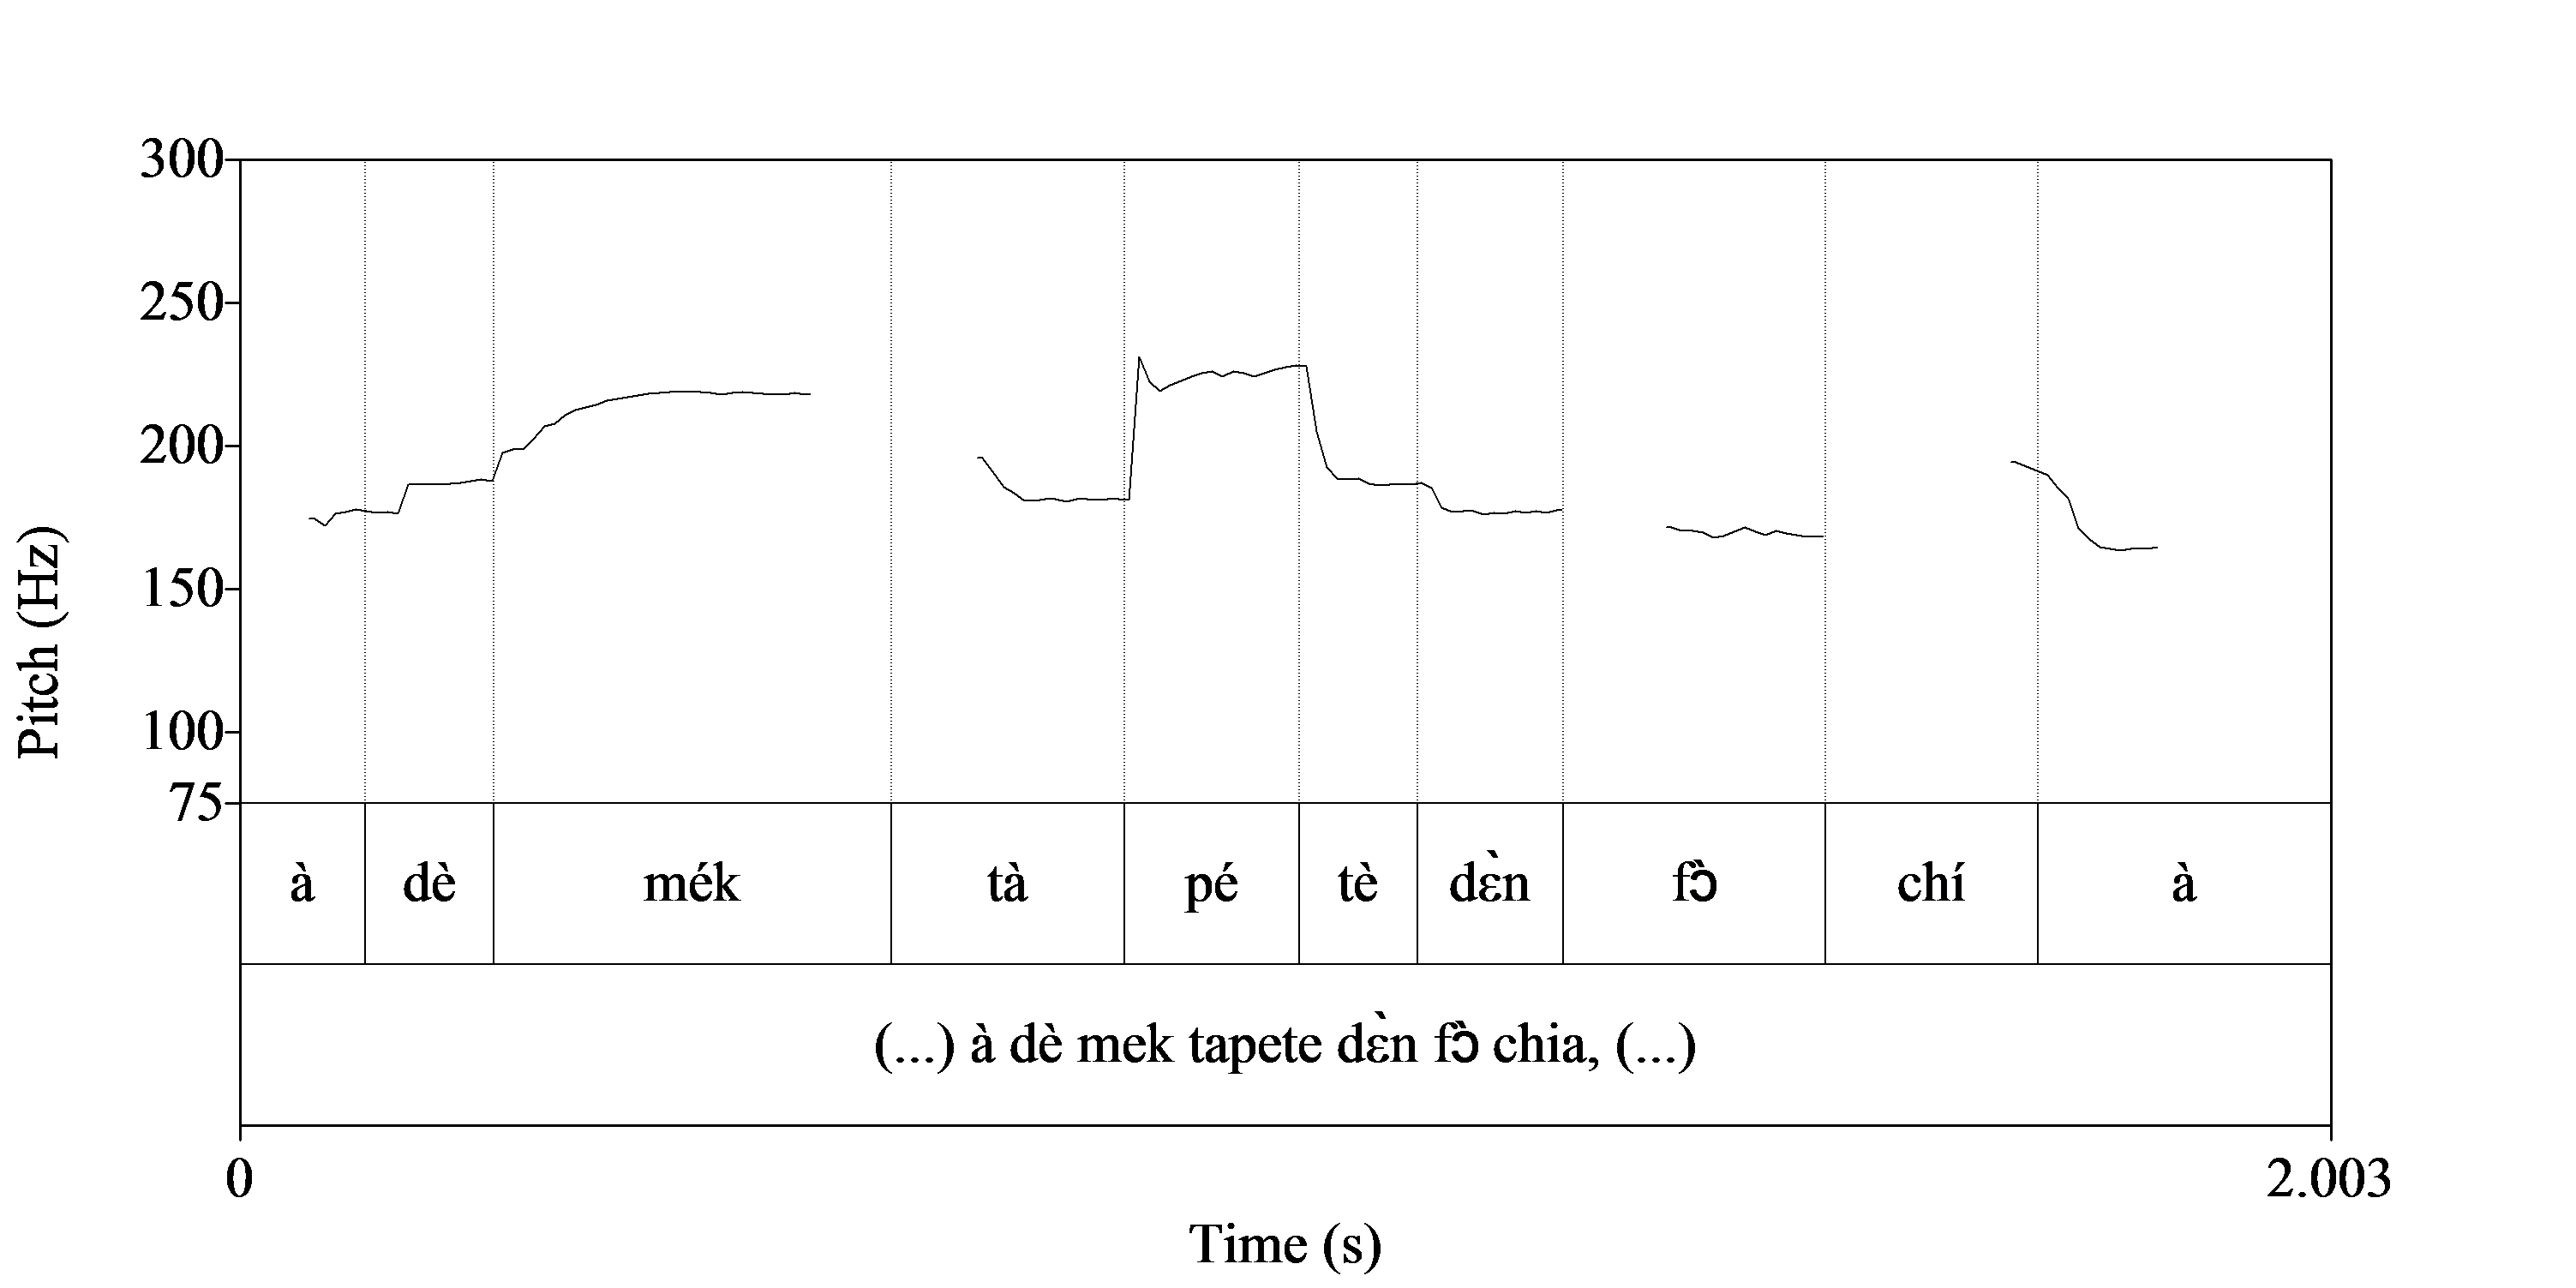
\includegraphics[height=.3\textheight]{figures/yakpomod-img39.png}
\end{figure}
 


\ea%90
    \label{ex:key:90}
    \glll   (...)  a    de  mék    tapete  dɛn  fɔ  chía, (…)\\
{}  \textsc{l}    \textsc{l}  \textsc{h}    \textsc{l.h.l}    \textsc{l}  \textsc{l}  \textsc{h.}\textbf{\textsc{lh\%}}\\
{}  \textsc{1sg.sbj}  \textsc{ipfv}  make  cloth  \textsc{pl}  \textsc{prep}  chair\\
\glt ‘(...)  I was making chair-drapings, (...)’
\z

\begin{figure}
\caption{Declarative L\% over final item in list\is{declarative intonation}}
\label{fig:key:3.38}
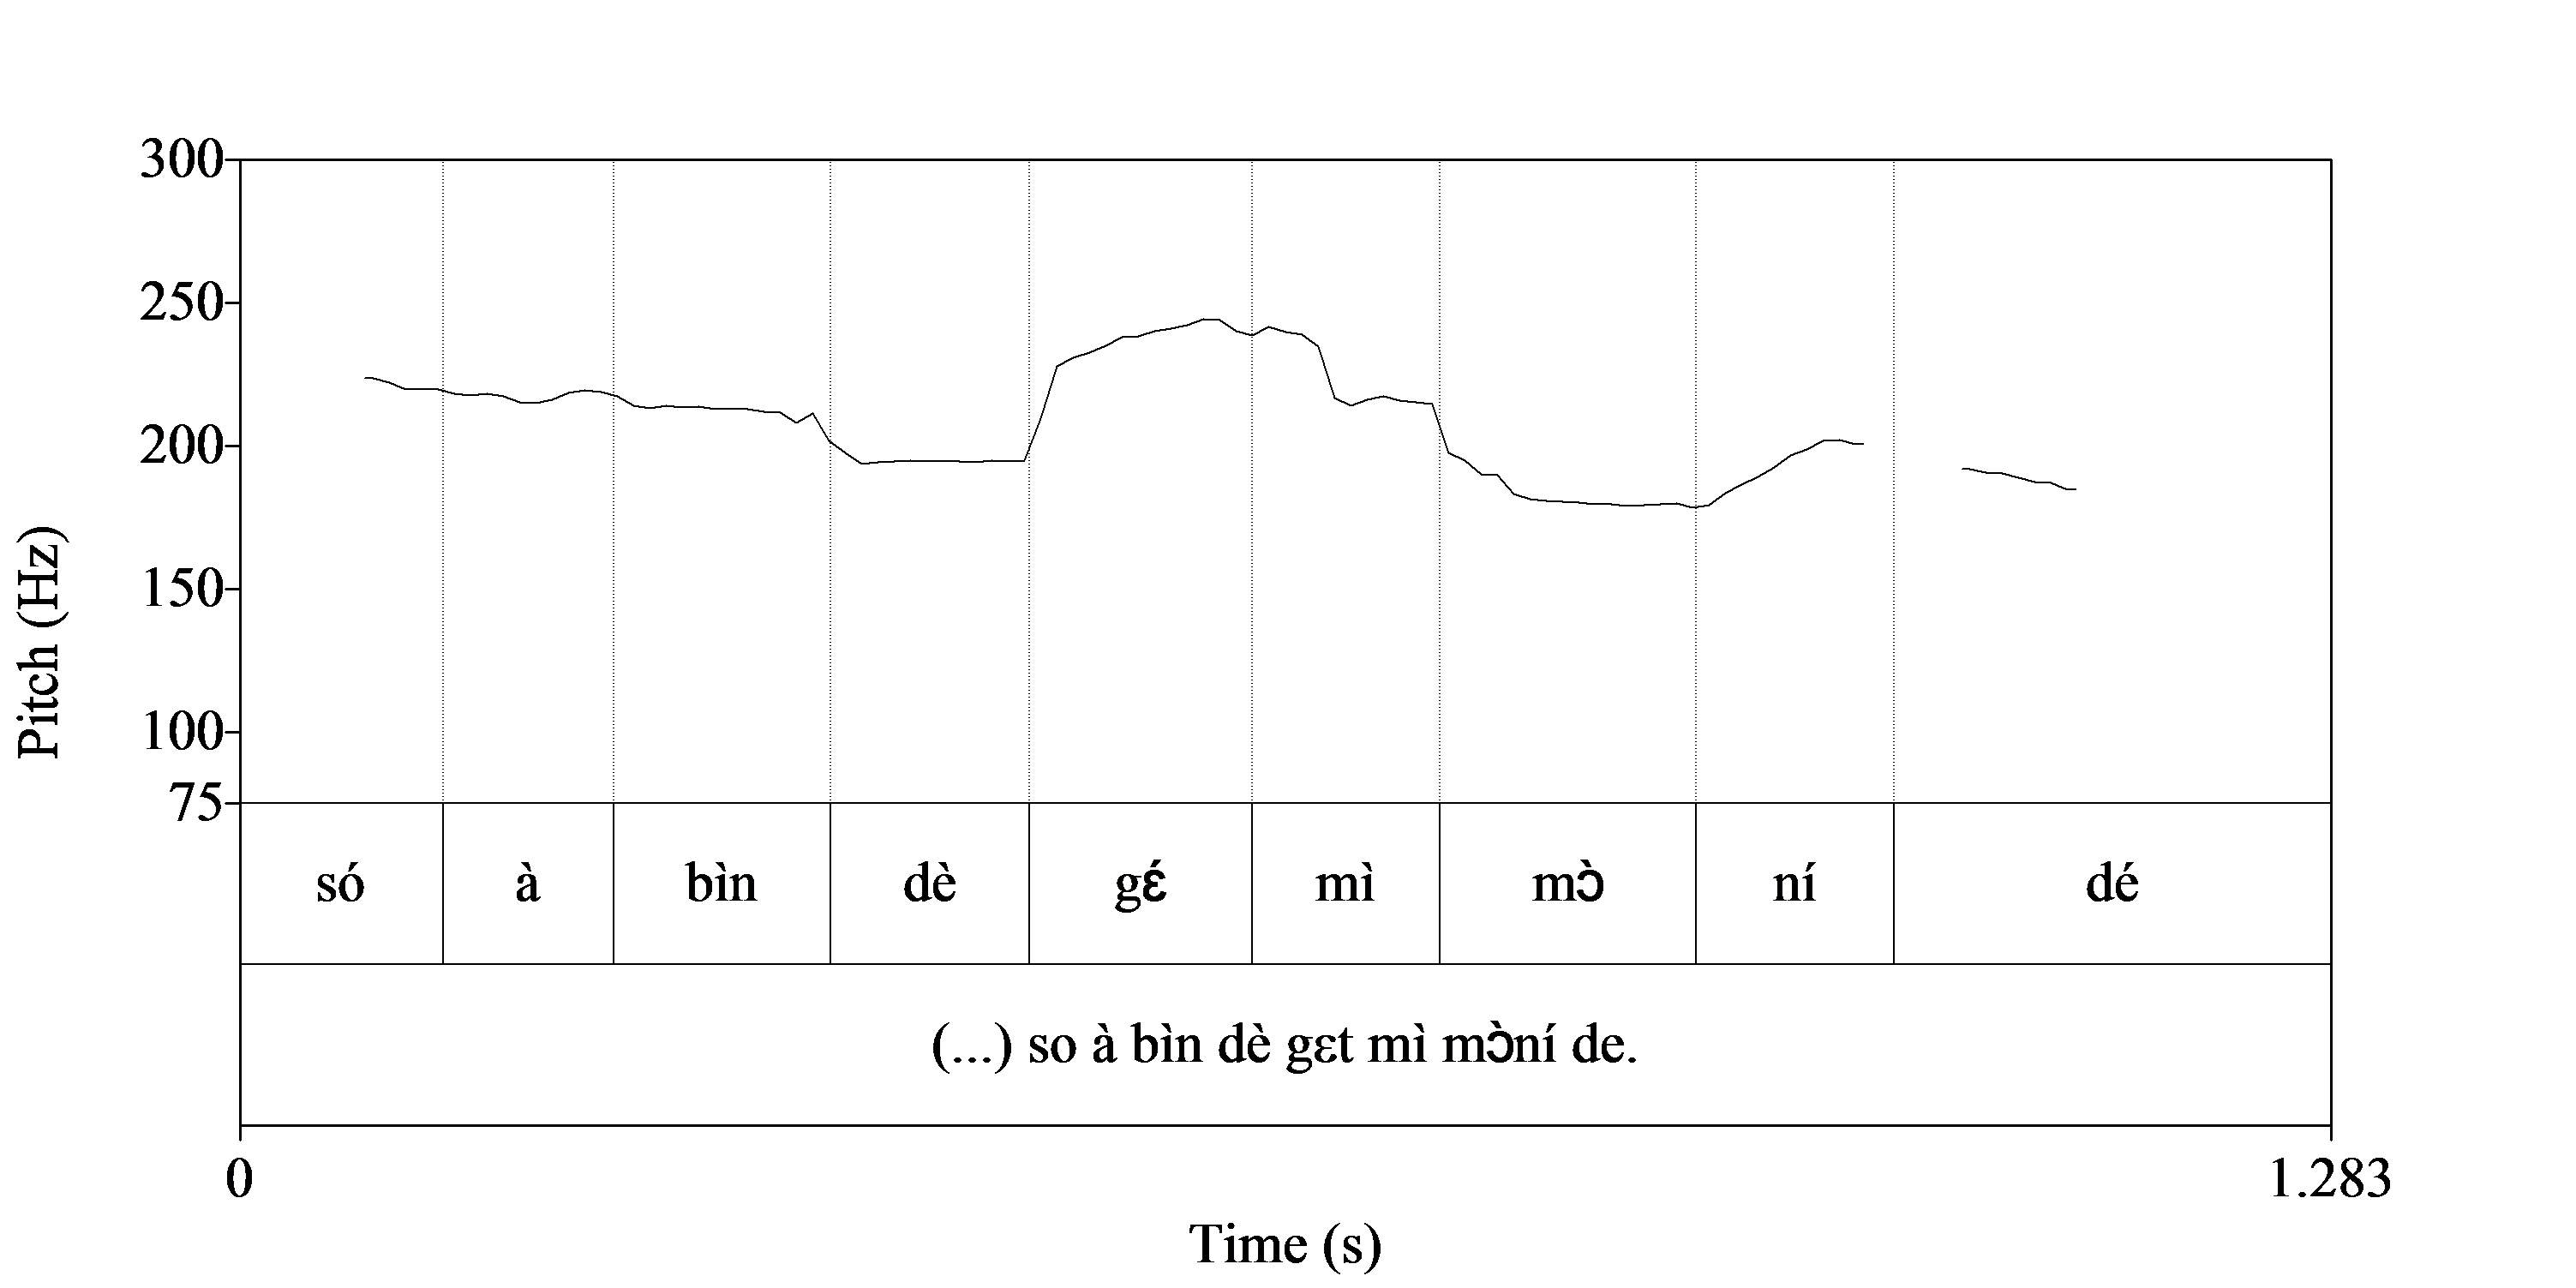
\includegraphics[height=.3\textheight]{figures/yakpomod-img40.png}
\end{figure}

  
 


\ea%91
    \label{ex:key:91}
    \glll   (...)  só  a    bin  dé  gɛ́t  mí    mɔní  dé.\\
  \textsc{h}  \textsc{l}    \textsc{l}  \textsc{l}  \textsc{h}  \textsc{l}    \textsc{l.h}    \textsc{h}\textbf{\textsc{l\%}}\\
  so  \textsc{1sg.sbj}  \textsc{pst}  \textsc{ipfv}  get  \textsc{1sg.poss}  money  there\\
\glt ‘(...) so I was getting my money there.’\is{list intonation}
\z


\subsection{Continuative intonation}\label{sec:3.4.4}

The absence of a boundary tone, usually before a prosodic break (a brief but audible pause), signals continuative intonation. With continuative intonation, the lexical tone of the relevant syllable simply maintains its pitch and is therefore pronounced with the same pitch as it would in utterance-medial position. Continuative intonation functions as a floor-holding device, a juncture marker on the right edge of utterances in order to prepare the ground for following material. Continuative intonation therefore plays an important role in signalling topic and focus next to the particles employed for this purpose (cf. \sectref{sec:7.4}). 


In \figref{fig:key:3.39}, the topical \textsc{NP} \textit{mi láyf} ‘my life’ is set off from the rest of the utterance by a pause. The monosyllable \textit{láyf} ‘life’ bears continuative intonation. Compare this to the utterance-final monosyllable \textit{bád} ‘bad’, which features declarative intonation, signalled by L\%\is{declarative intonation}. The symbol [p] indicates a pause. The pitch trace of the pronoun \textit{è} ‘\textsc{3sg.sbj}’ is slighty distorted due to creaky voice: 


\begin{figure}
\caption{Continuative intonation with topicalisation}
\label{fig:key:3.39}
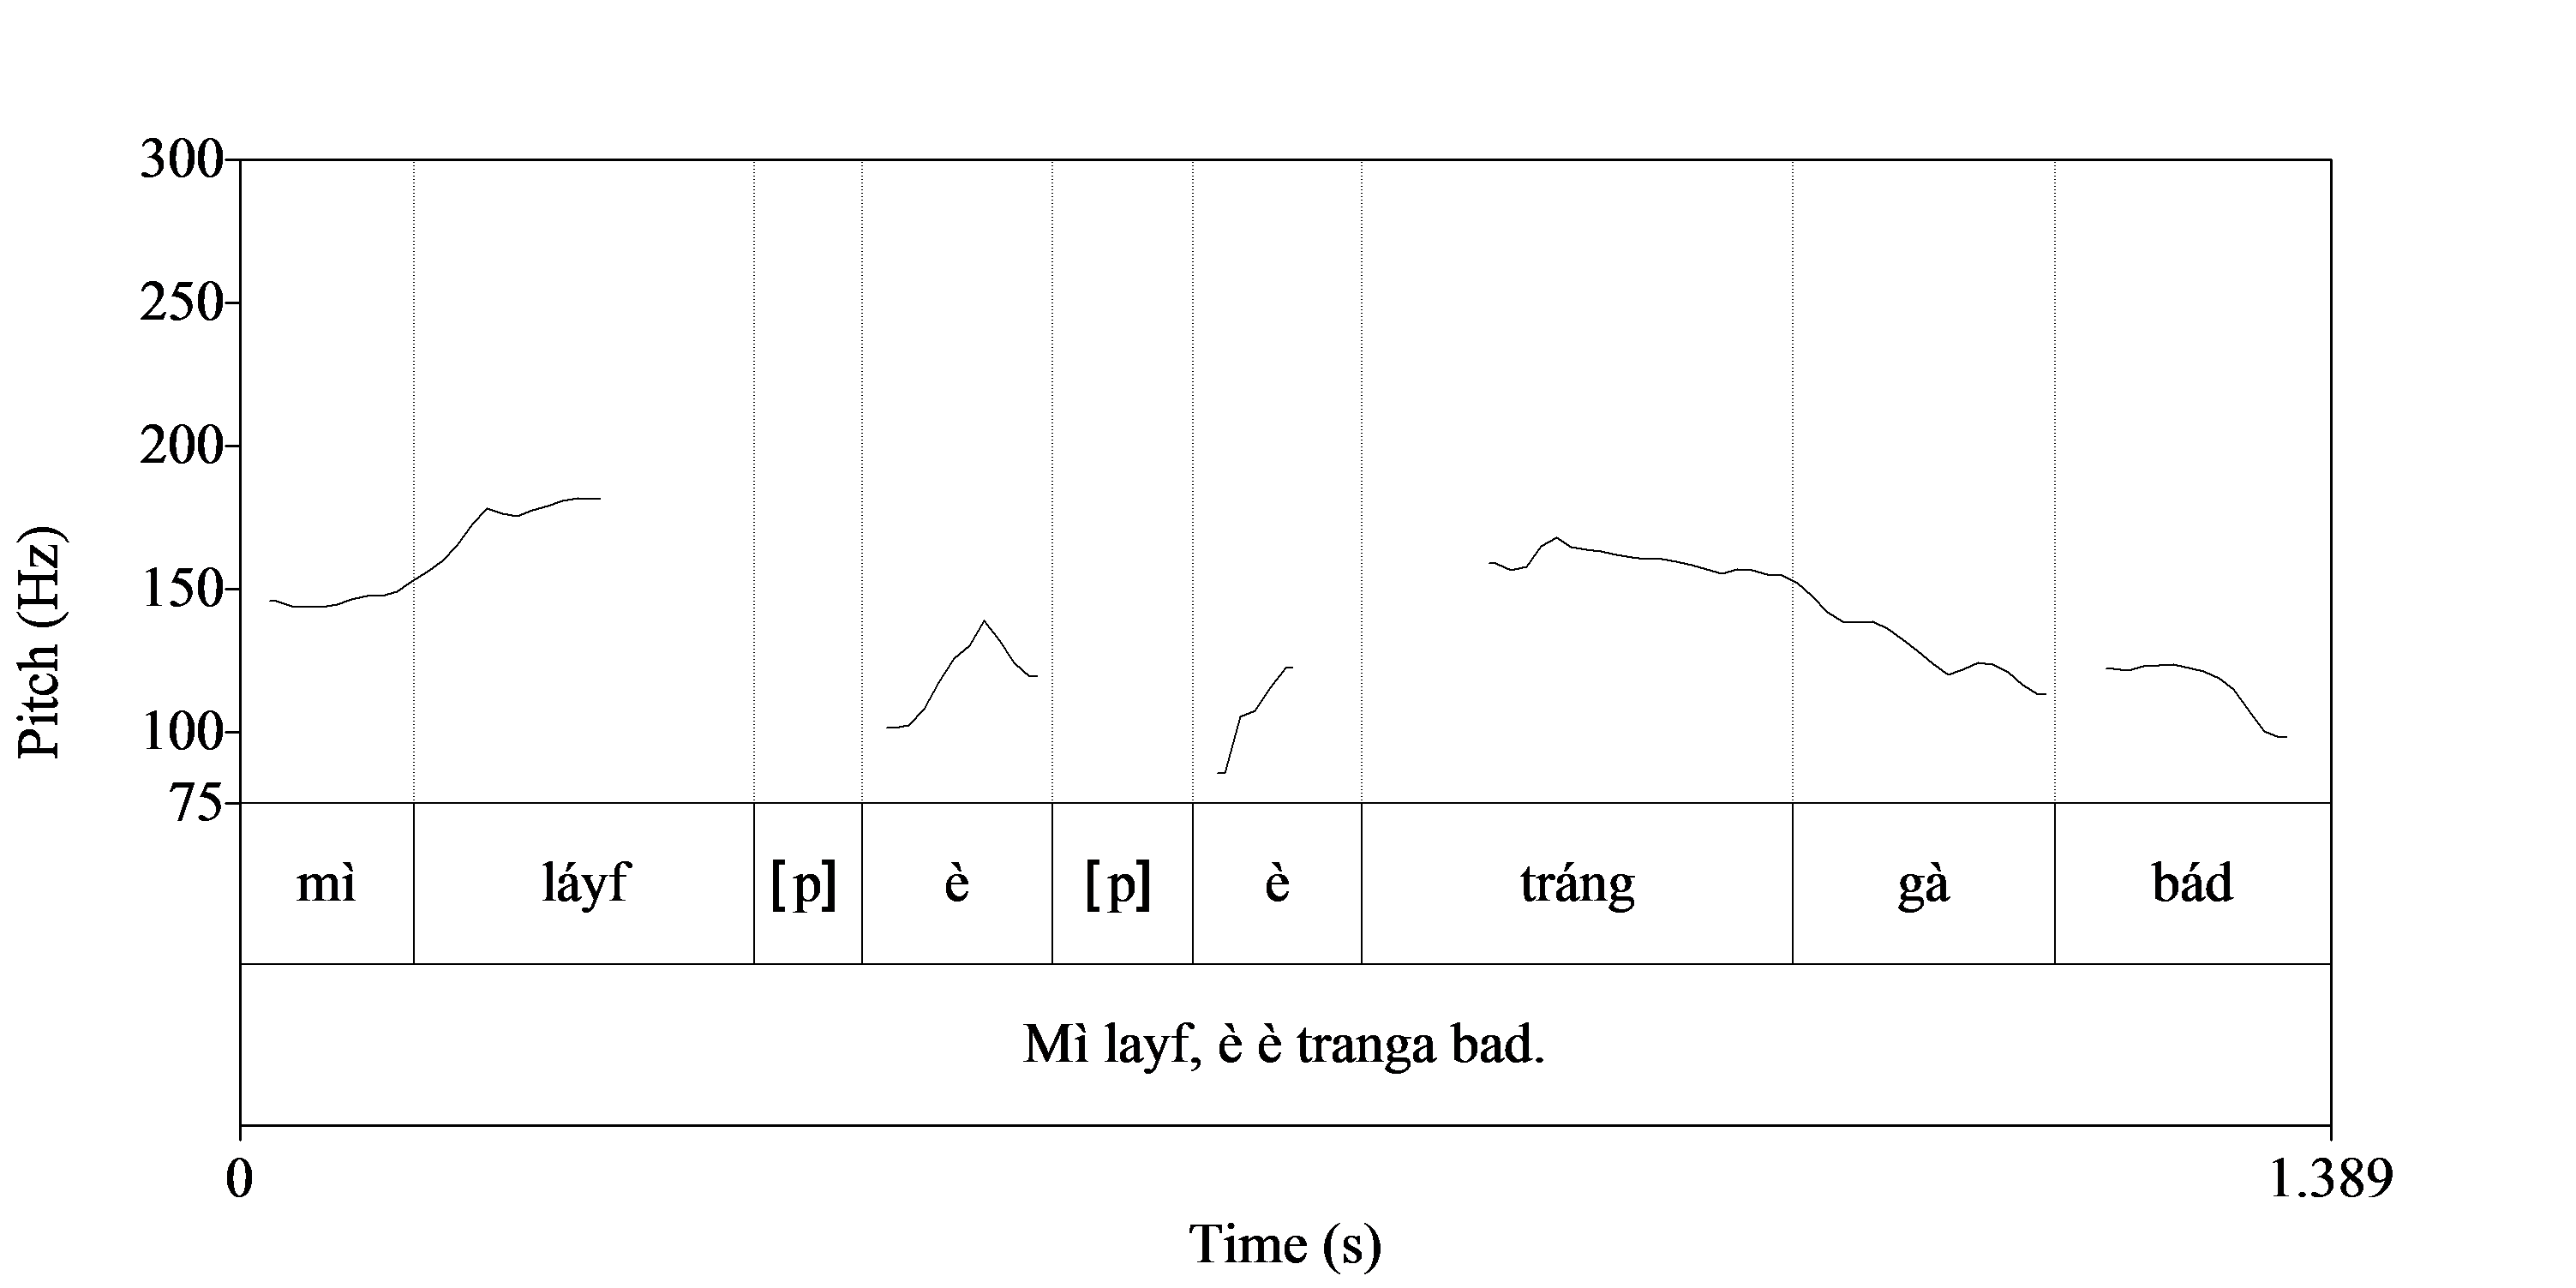
\includegraphics[height=.3\textheight]{figures/yakpomod-img41.png}
\end{figure}

  
 
\ea\label{ex:key:92}
\glll Mi \textstylePichiexamplebold{láyf},  e,    e    tránga \textbf{bád}.\\
\textsc{l}    \textsc{h}\textbf{\textsc{${\emptyset}$}}\textbf{\textsc{\%}  }  \textsc{l}    \textsc{l}    \textsc{h.l}      \textsc{h}\textbf{\textsc{l\%}}\\
\textsc{1sg.poss}  life    \textsc{3sg.sbj}  \textsc{3sg.sbj}  be.strong  extremely\\
\glt ‘My life, it, it was really tough.’    
\z

Continuative intonation is also employed as a juncture marker between linked clauses. Here, it may occur alone as a prosodic clause linker between juxtaposed clauses, or in conjunction with an overt clause linker. \figref{fig:key:3.40} and \figref{fig:key:3.41} are two clauses linked in a sequential, temporal relation. The adverbial time clause is introduced by \textit{di} \textit{dé} \textit{wé} ‘(the day) when’ in \figref{fig:key:3.40}. In the example, continuative intonation is found over the rightmost L-toned monosyllable \textit{=an} ‘\textsc{3sg.obj}’. The absence of the utterance-final L\% of declarative intonation halts the fall of the lexical L tone to the bottom of the pitch register:

\begin{figure}
\caption{Continuative intonation with clause linkage} 
\label{fig:key:3.40}
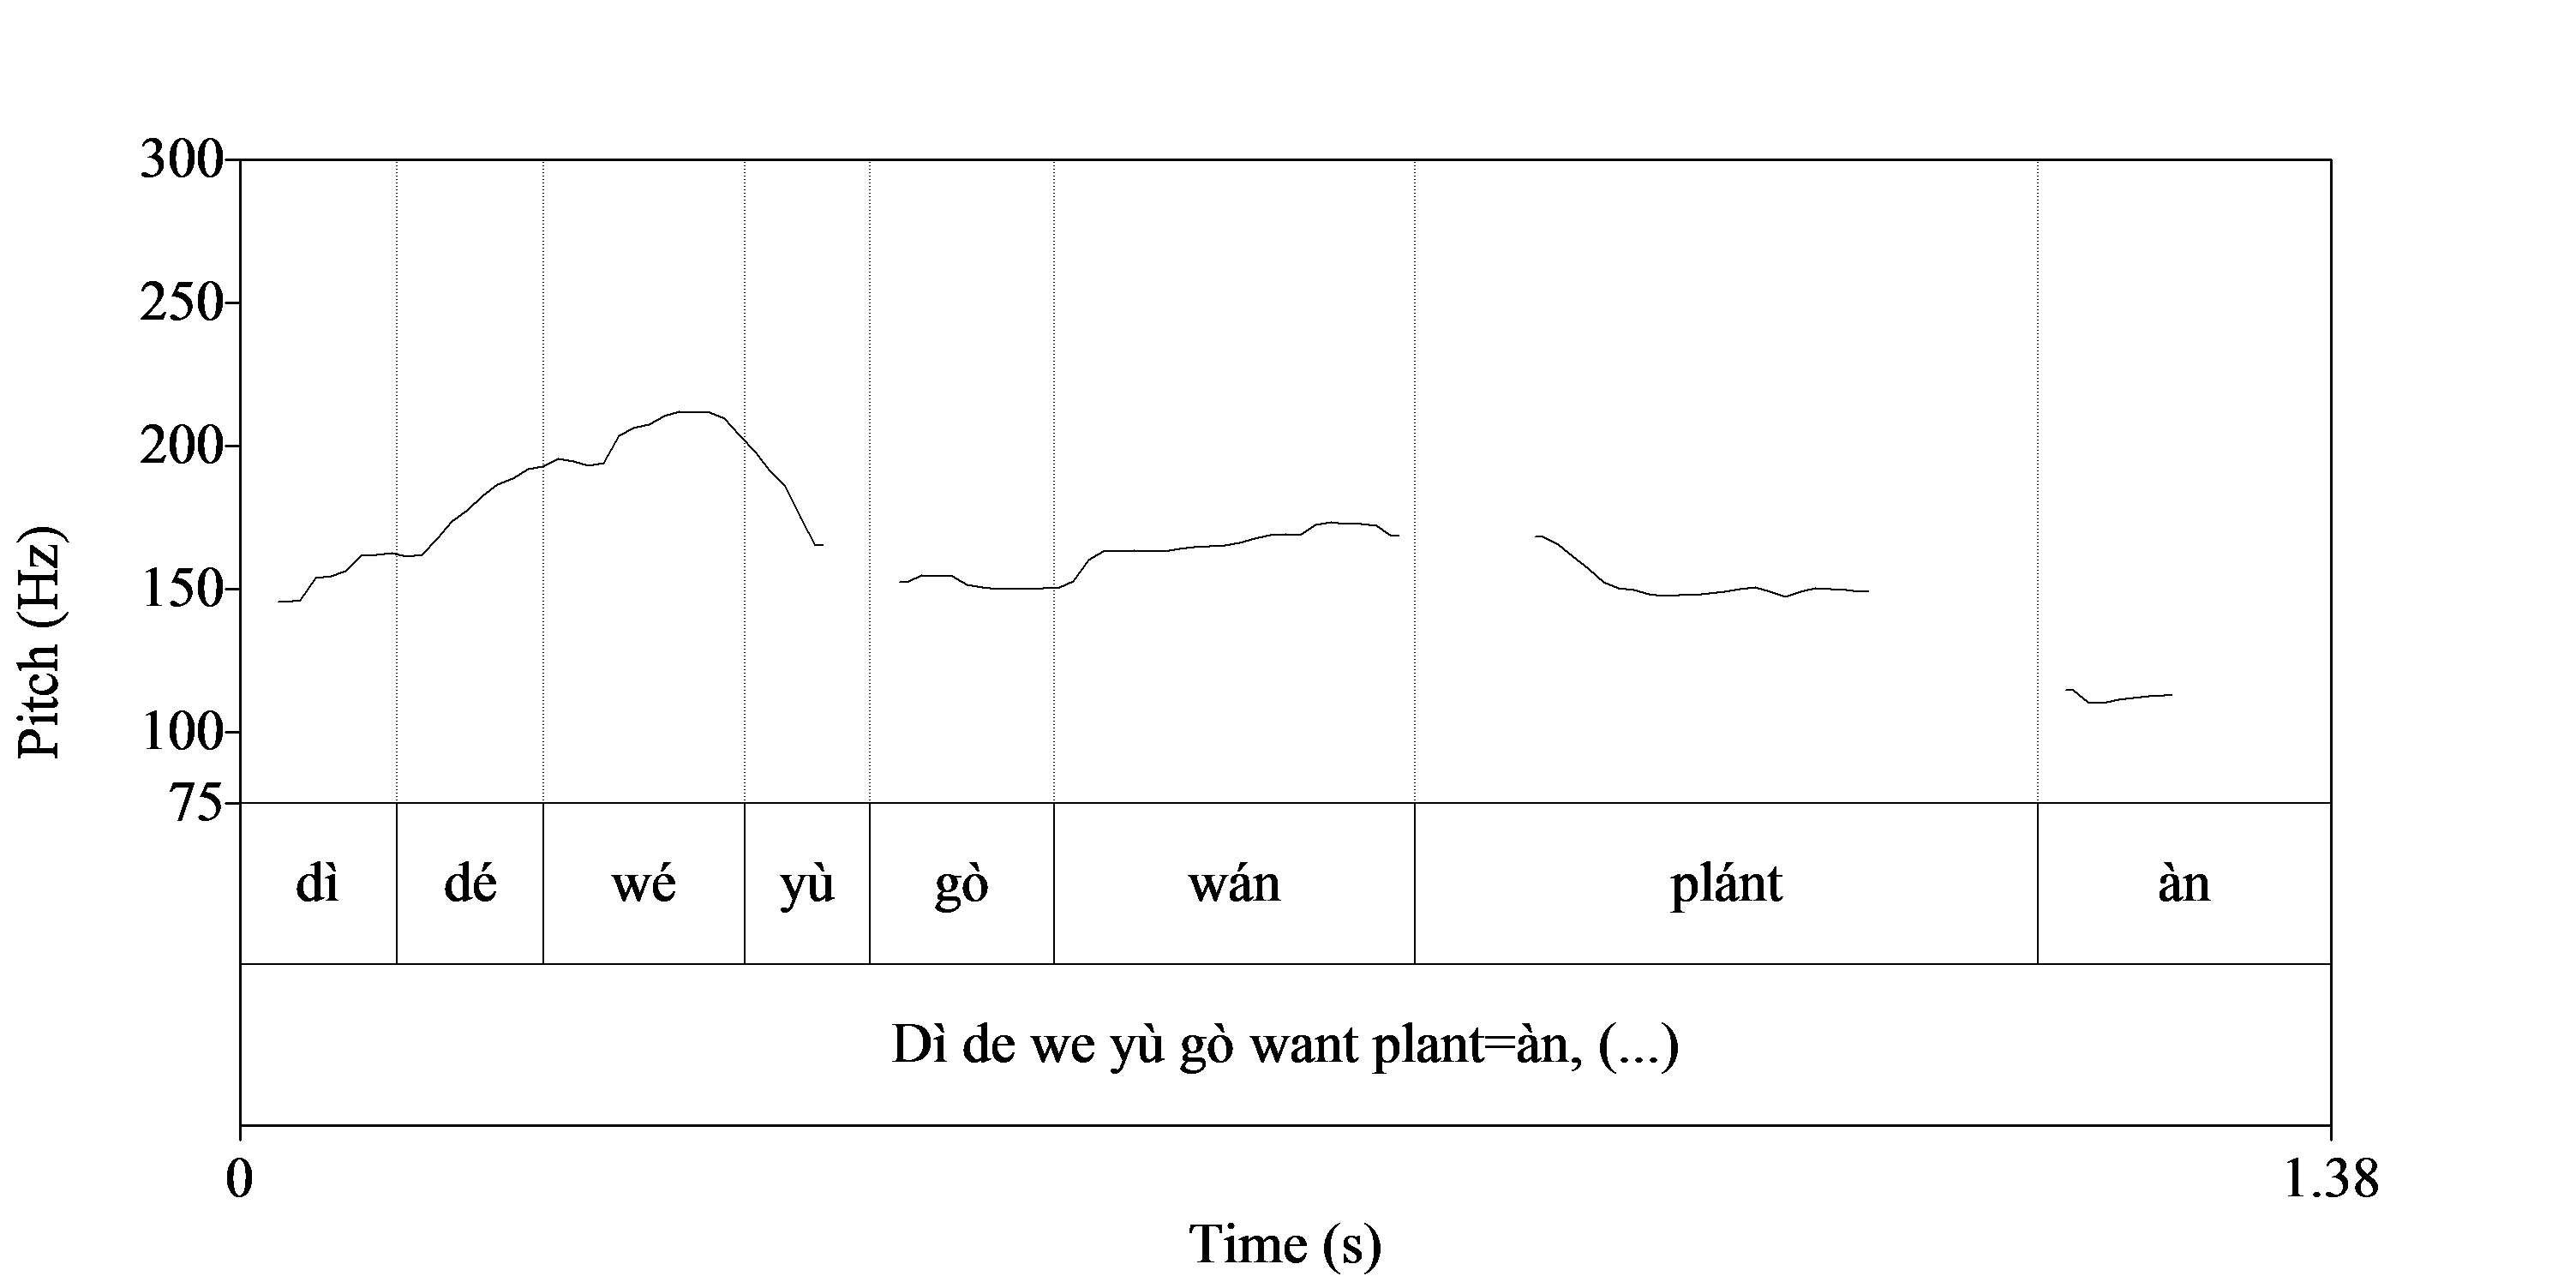
\includegraphics[height=.3\textheight]{figures/yakpomod-img42.png}
\end{figure}

\ea%93
    \label{ex:key:93}
    \glll   Di  dé  wé  yu  go  wánt  plánt=an,  (...)\\
\textsc{l}  \textsc{h}  \textsc{h}  \textsc{l}  \textsc{l}  \textsc{h}    \textsc{h=l}\textbf{\textsc{${\emptyset}$}}\textbf{\textsc{\%}}\\
\textsc{def}  day  \textsc{sub}  \textsc{2sg}  \textsc{pot}  want  plant=\textsc{3sg.obj}\\
\glt ‘The day you would want to go plant it (...)’      
\z

The second clause in sequence features a lexical H over the utterance-final syllable. Here, continuative intonation produces no effect other than the maintenance of the lexical H tone. Compare \textit{dɔtalɔ́} ‘daughter-in-law’ and \textit{sɔnilɔ́} ‘son-in-law’ in \figref{fig:key:3.41}: 

\begin{figure}
\caption{Continuative intonation over non-final clause}
\label{fig:key:3.41}
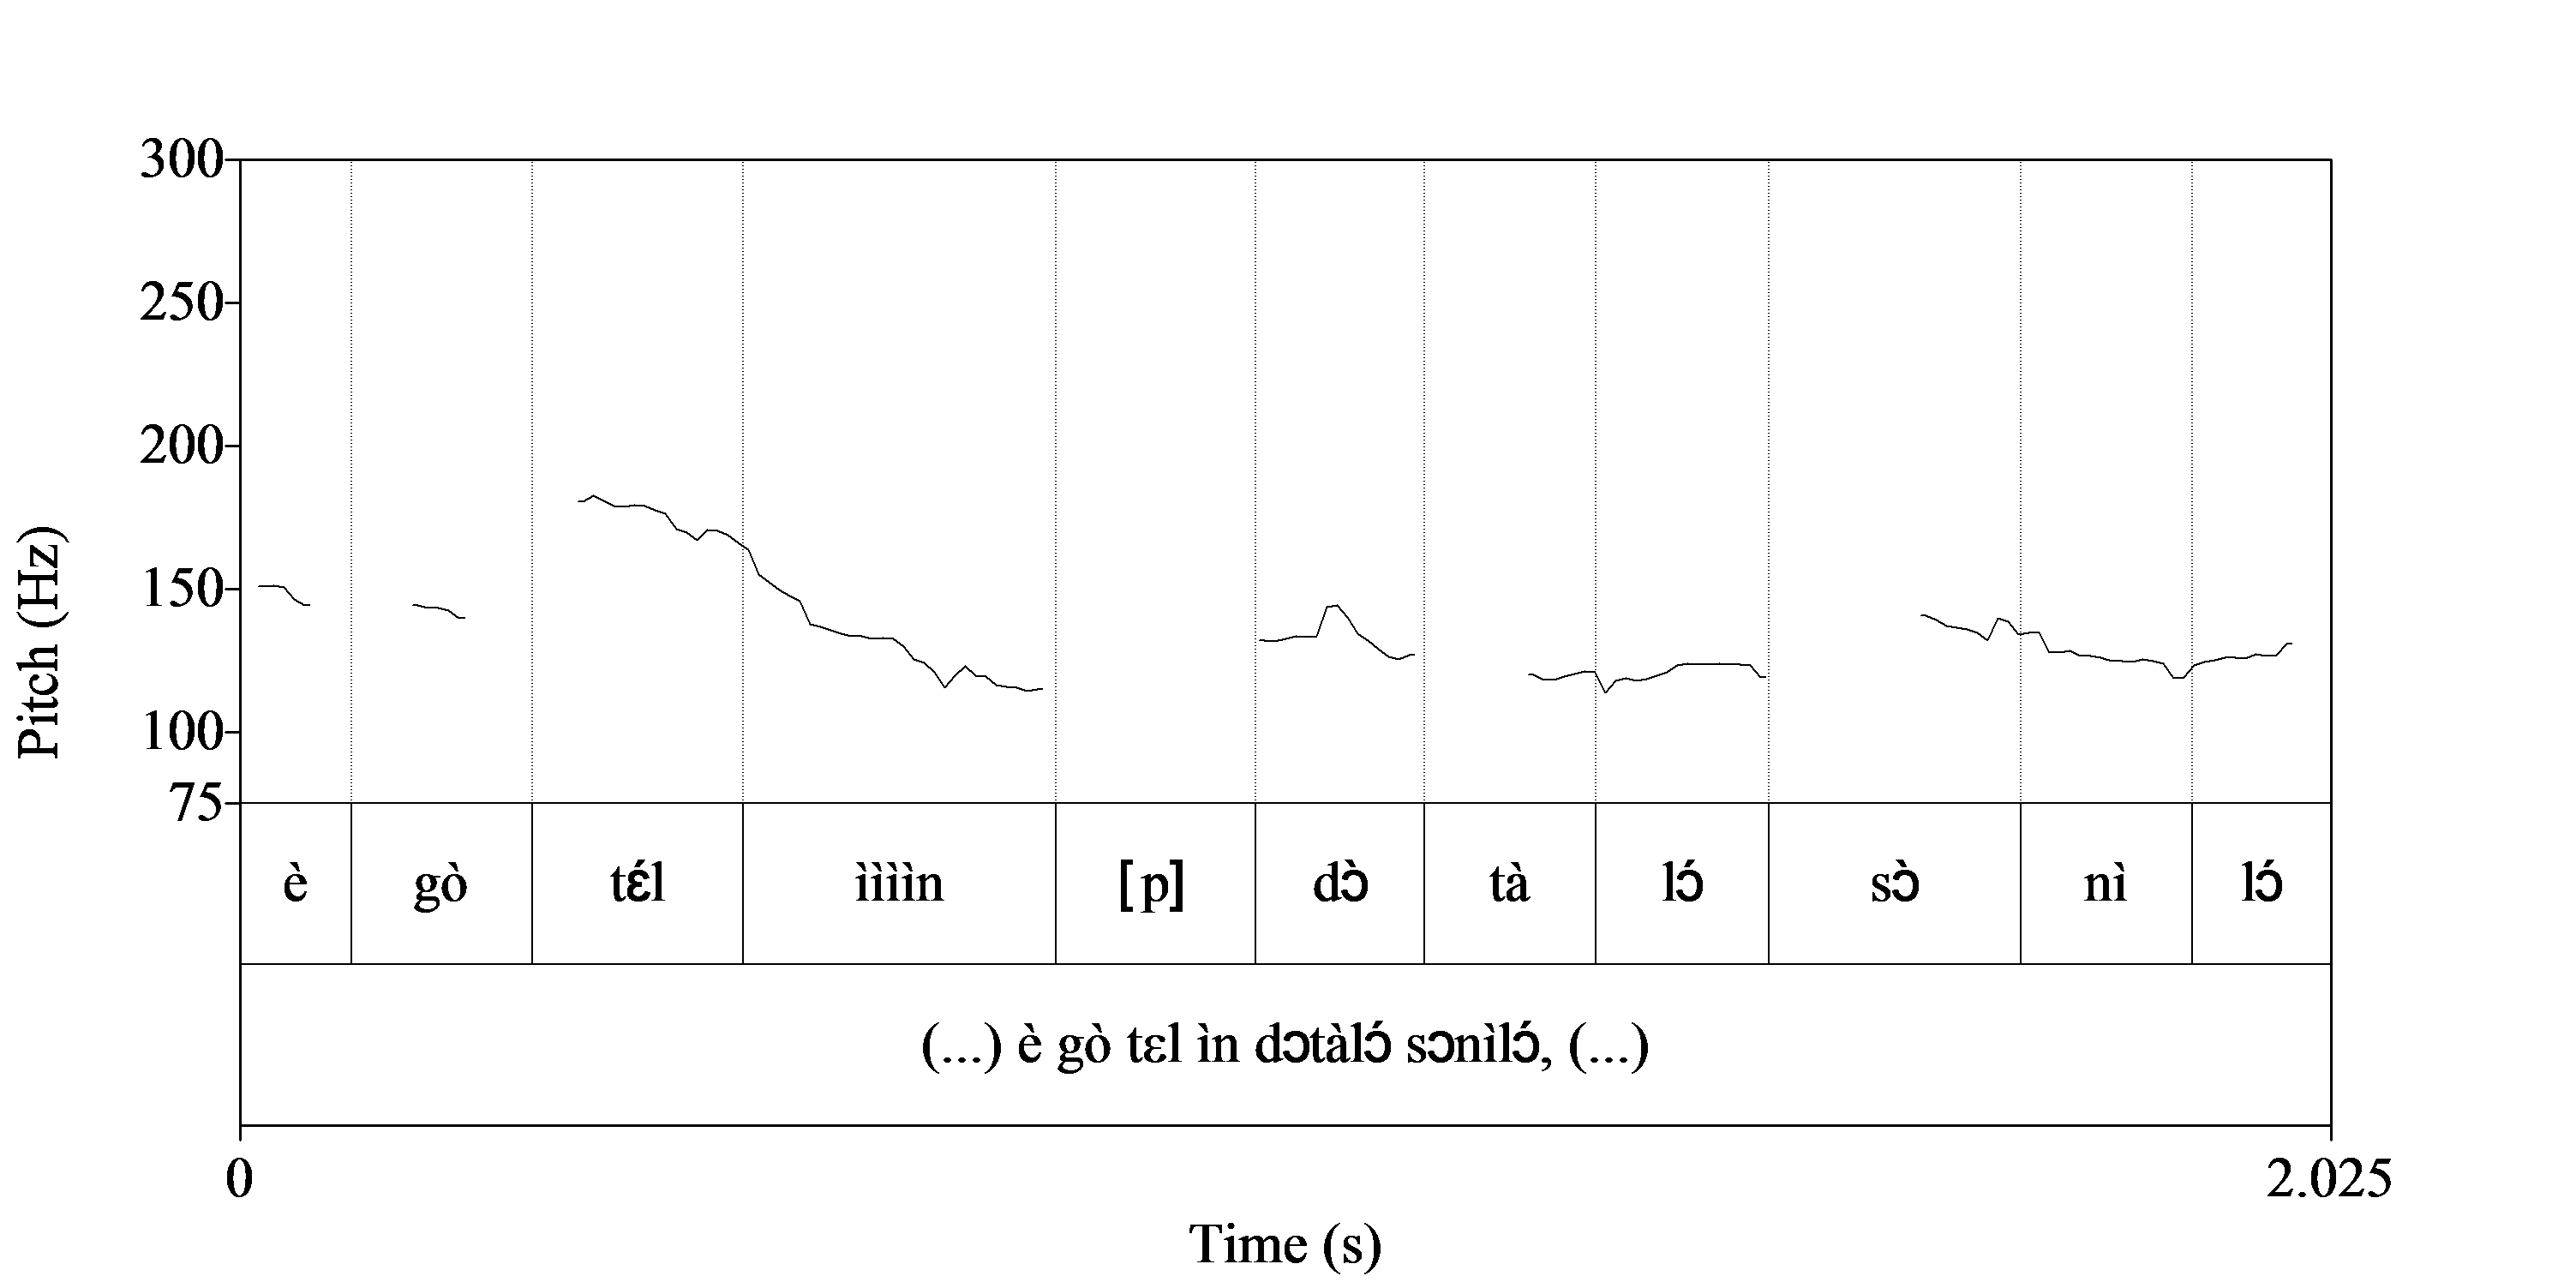
\includegraphics[height=.3\textheight]{figures/yakpomod-img43.png}
\end{figure}

\ea%94
    \label{ex:key:94}
    \glll   E    go  tɛ́l  in    dɔtalɔ́,      sɔnilɔ́,  (...)\\
\textsc{l}    \textsc{l}  \textsc{h}  \textsc{l}    \textsc{l.l.h}\textbf{\textsc{${\emptyset}$}}\textbf{\textsc{\%}}      \textsc{l.l.h}\textbf{\textsc{${\emptyset}$}}\textbf{\textsc{\%}}\\
\textsc{3sg.sbj}  \textsc{pot}  tell  \textsc{3sg.poss}  daughter-in-law  son-in-law\\
\glt ‘She would tell her daughter-in-law, son-in-law, (...)’  
\z


Continuative intonation is also used as a stylistic device in ‘unfinished’\textstyleannotationreference{} utterances, such as the one in \figref{fig:key:3.42}. The final syllable retains its H tone or may even rise slightly towards the end. This emphatic variant of declarative\is{declarative intonation:emphatic} intonation is employed for dramatic effect. Compare the utterance-final, H-toned monosyllable \textit{dé} ‘there’: 

\begin{figure}
\caption{Continuative intonation for stylistic effect}
\label{fig:key:3.42}
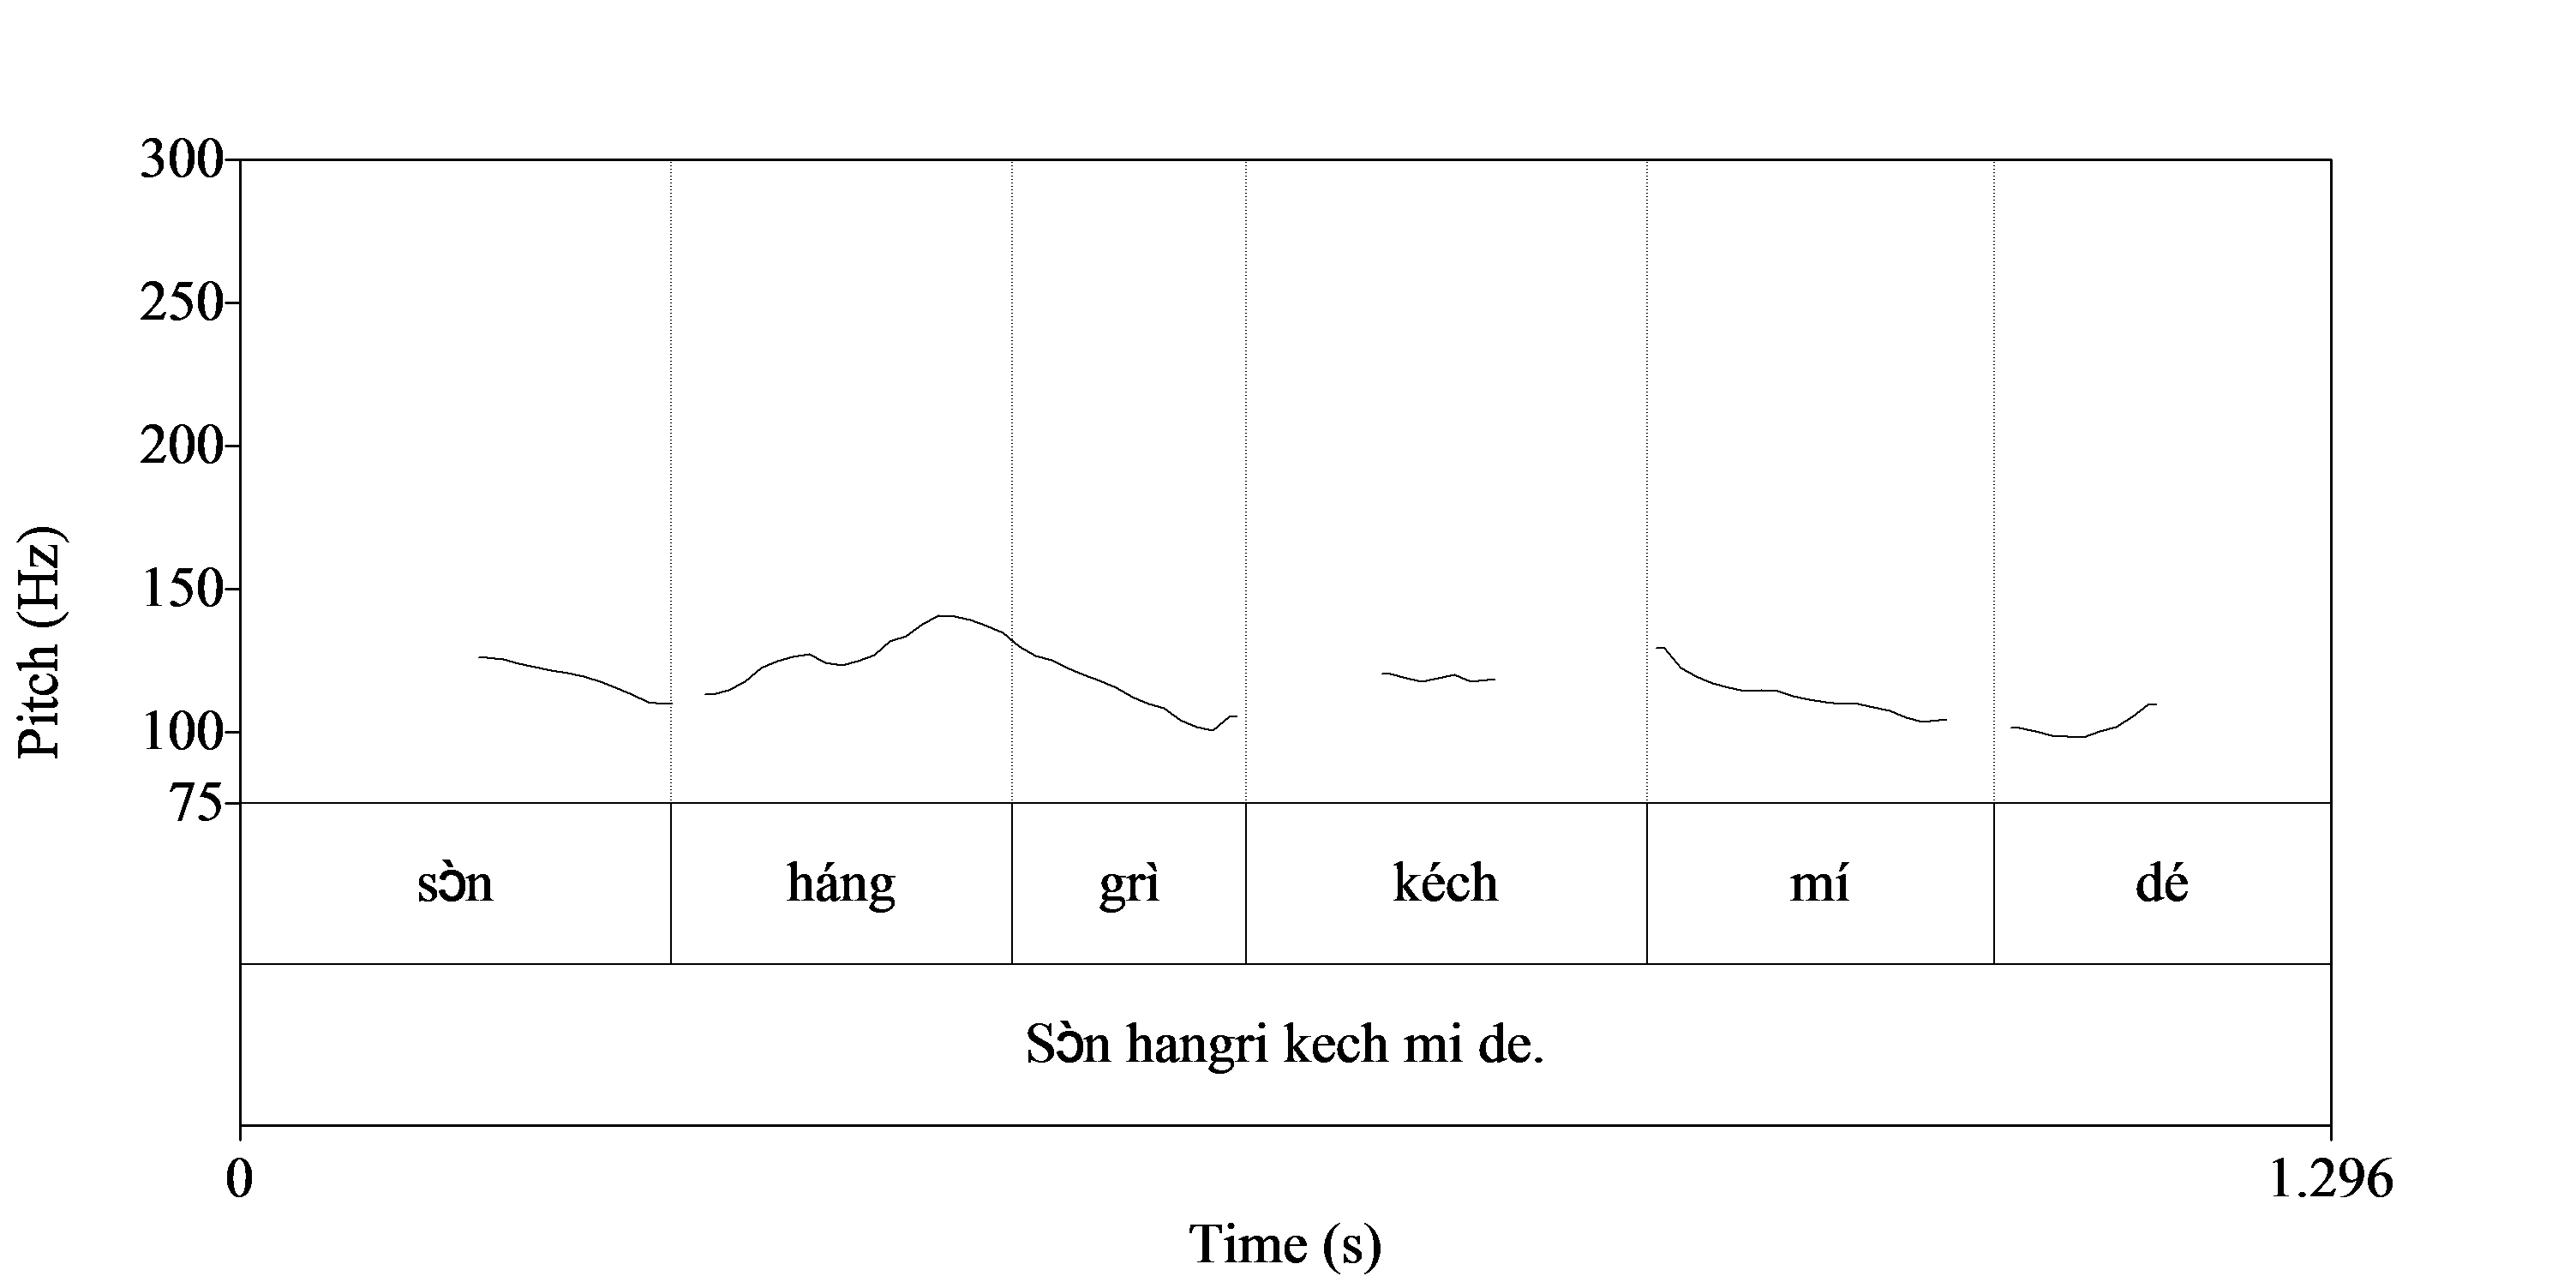
\includegraphics[height=.3\textheight]{figures/yakpomod-img44.png}
\end{figure}

  
 


\ea%95
    \label{ex:key:95}
    \glll   Sɔn    hángri    kéch  mí    \textbf{dé}.\\
L    \textsc{h.l}      \textsc{h}    \textsc{h}    \textsc{h}\textbf{\textsc{${\emptyset}$}}\textbf{\textsc{\%}}\\
some  be.hungry  catch  \textsc{1sg.indp}  there\\
\glt ‘I became really hungry there [you wouldn’t believe how much].’\is{continuative intonation}
\z

\subsection{Question intonation}\label{sec:3.4.5}

Yes–no questions are formed with an LH\% contour boundary tone. Contrary to emphatic intonation, question intonation is substitutive: The lexical tone over the utterance-final syllable is replaced by the question LH\%. In this way, the utterance-final syllable of a yes–no question invariably bears an LH contour, irrespective of its original tone. Compare the pitch contour over the L-toned second syllable of \textit{Píchi} ‘Pichi’ in \figref{fig:key:3.43}: 

\begin{figure}
\caption{Non-emphatic yes–no question}
\label{fig:key:3.43}
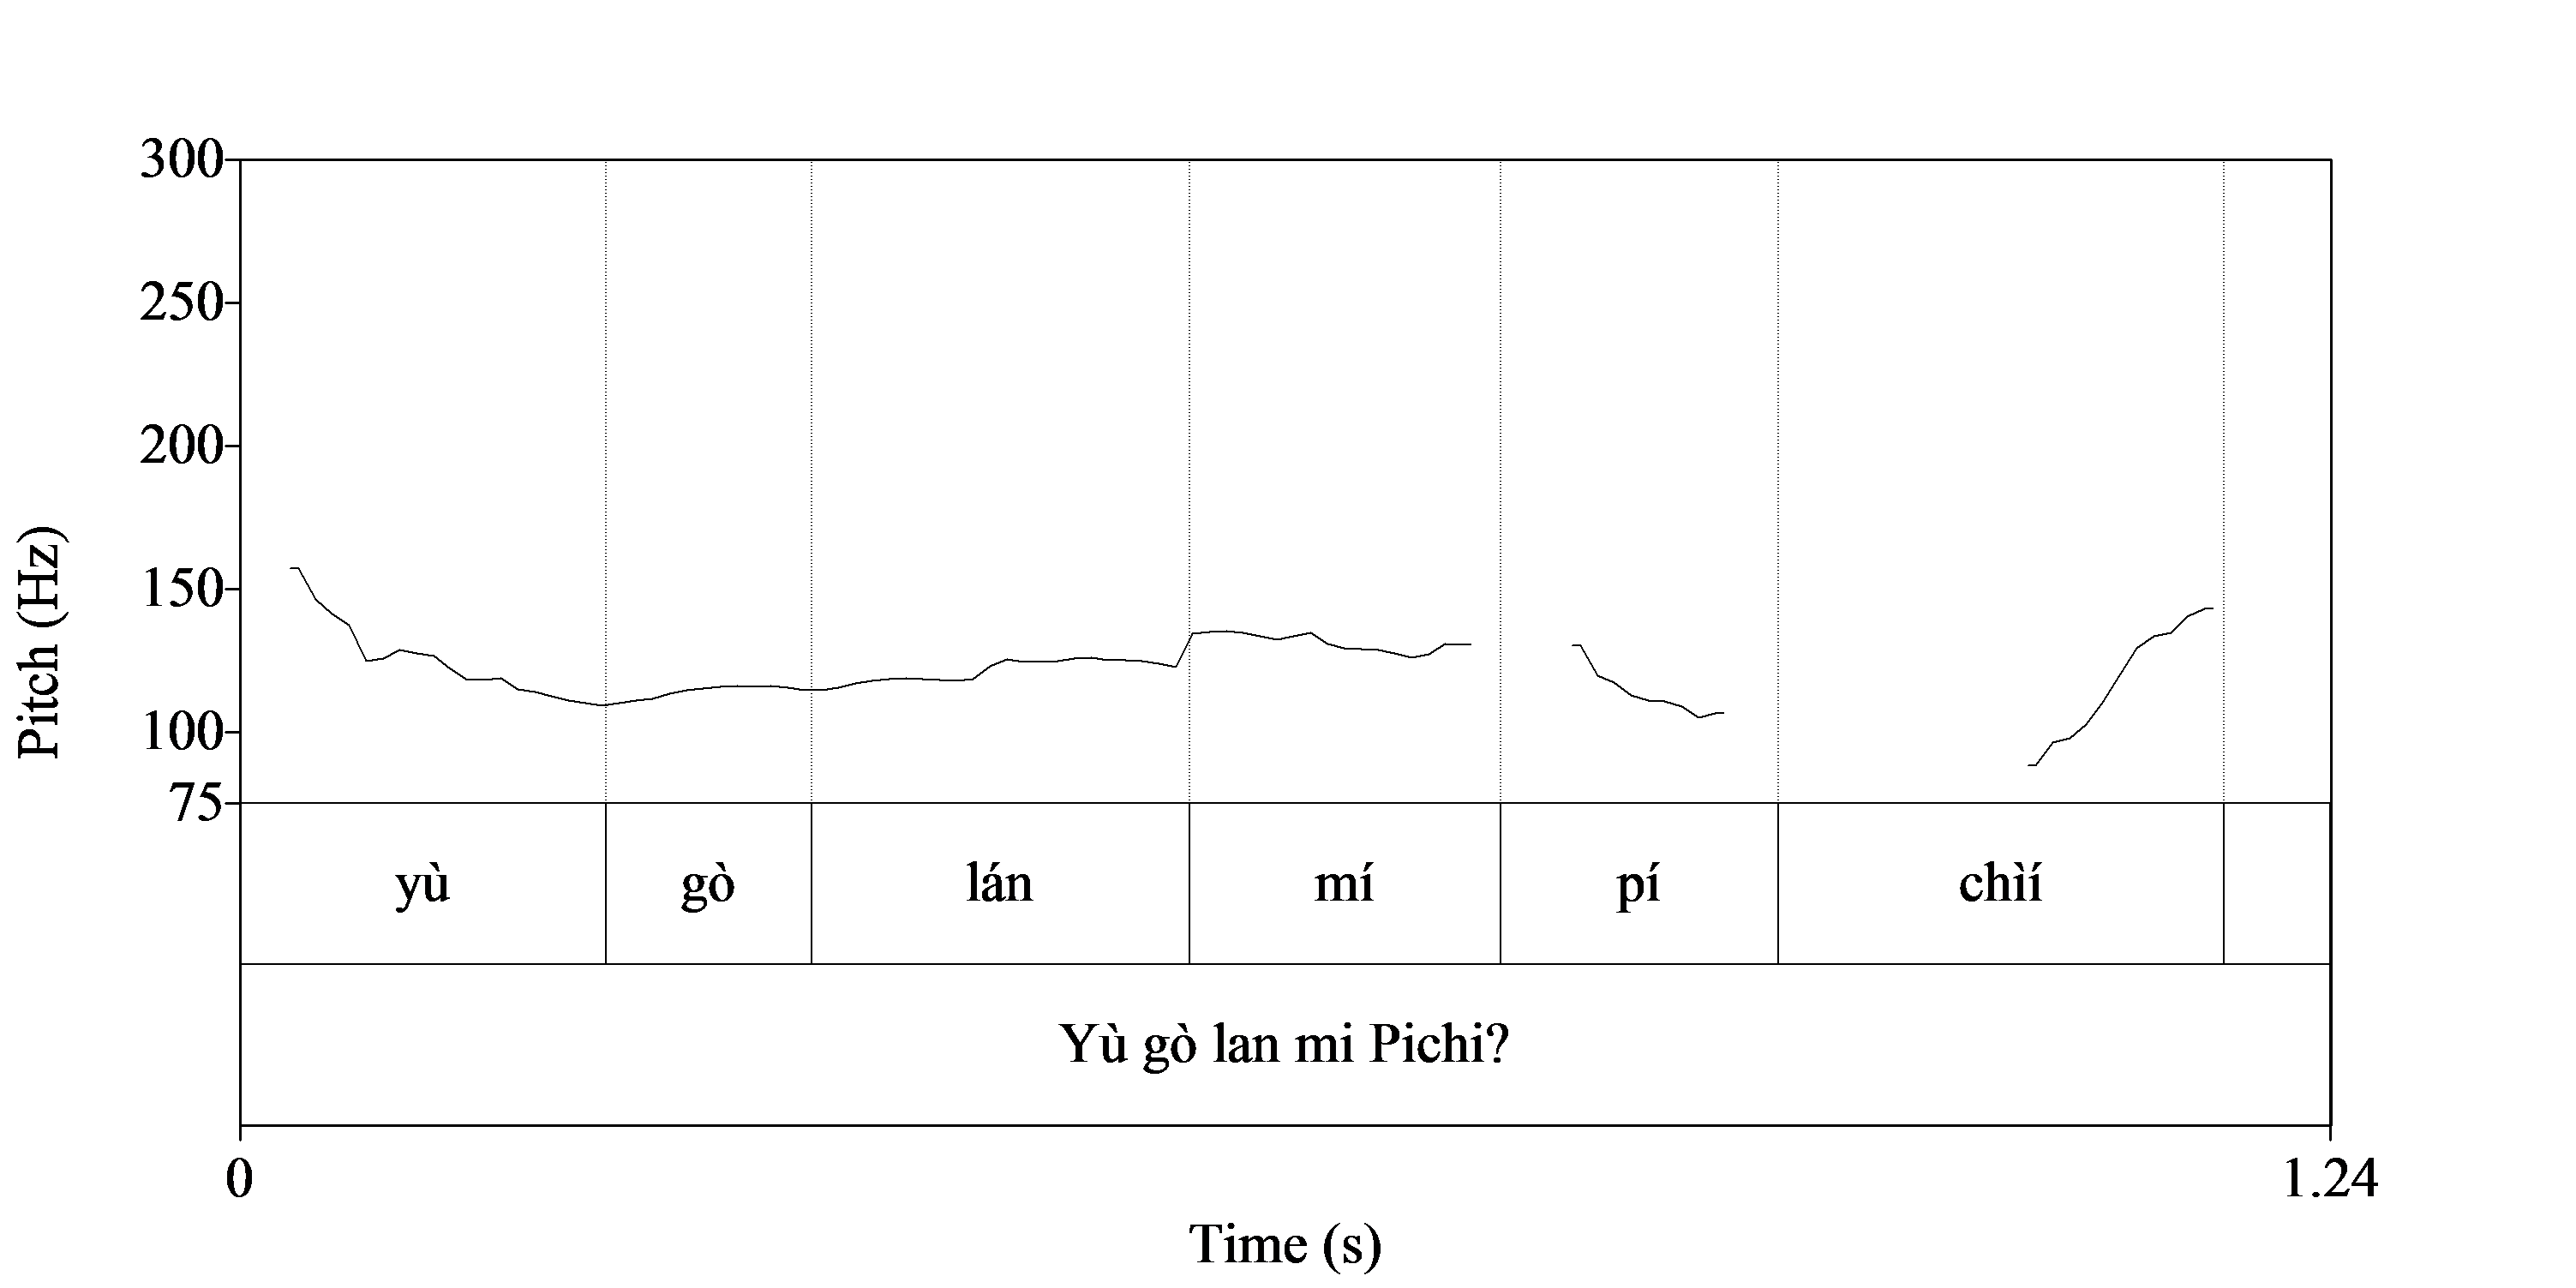
\includegraphics[height=.3\textheight]{figures/yakpomod-img45.png}
\end{figure}

  
 


\ea%96
    \label{ex:key:96}
    \glll   Yu    go    lán    mí    Píchi?\\
\textsc{l}    \textsc{l}    \textsc{h}    \textsc{h}    \textsc{h.}\textbf{\textsc{lh\%}}\\
\textsc{2sg}    \textsc{pot}    teach  \textsc{1sg.indp}  Pichi\\
\glt ‘Will you teach me Pichi?’  
\z

The H tone of the LH\% contour may vary in pitch. While non-emphatic questions exhibit a gentle final rise and may therefore be similar in pitch to continuative intonation\is{continuative intonation}, more emphatic questions yield steeper rises. The more dramatic the rise, the more the question may additionally convey emphatic nuances like counter-expectation or insistence. I assume that in instances where the rise is particularly steep, the H tone component of the LH\% boundary contour tone is raised to extra-high, thus rendering L+H\%. Such an extra-steep rise is particularly common in rhetorical questions, optionally over the L-toned utterance-final question tag \textit{nɔ́} as in the following example:\is{alternative questions} 

\begin{figure}
\caption{Emphatic yes–no question}
\label{fig:key:3.44}
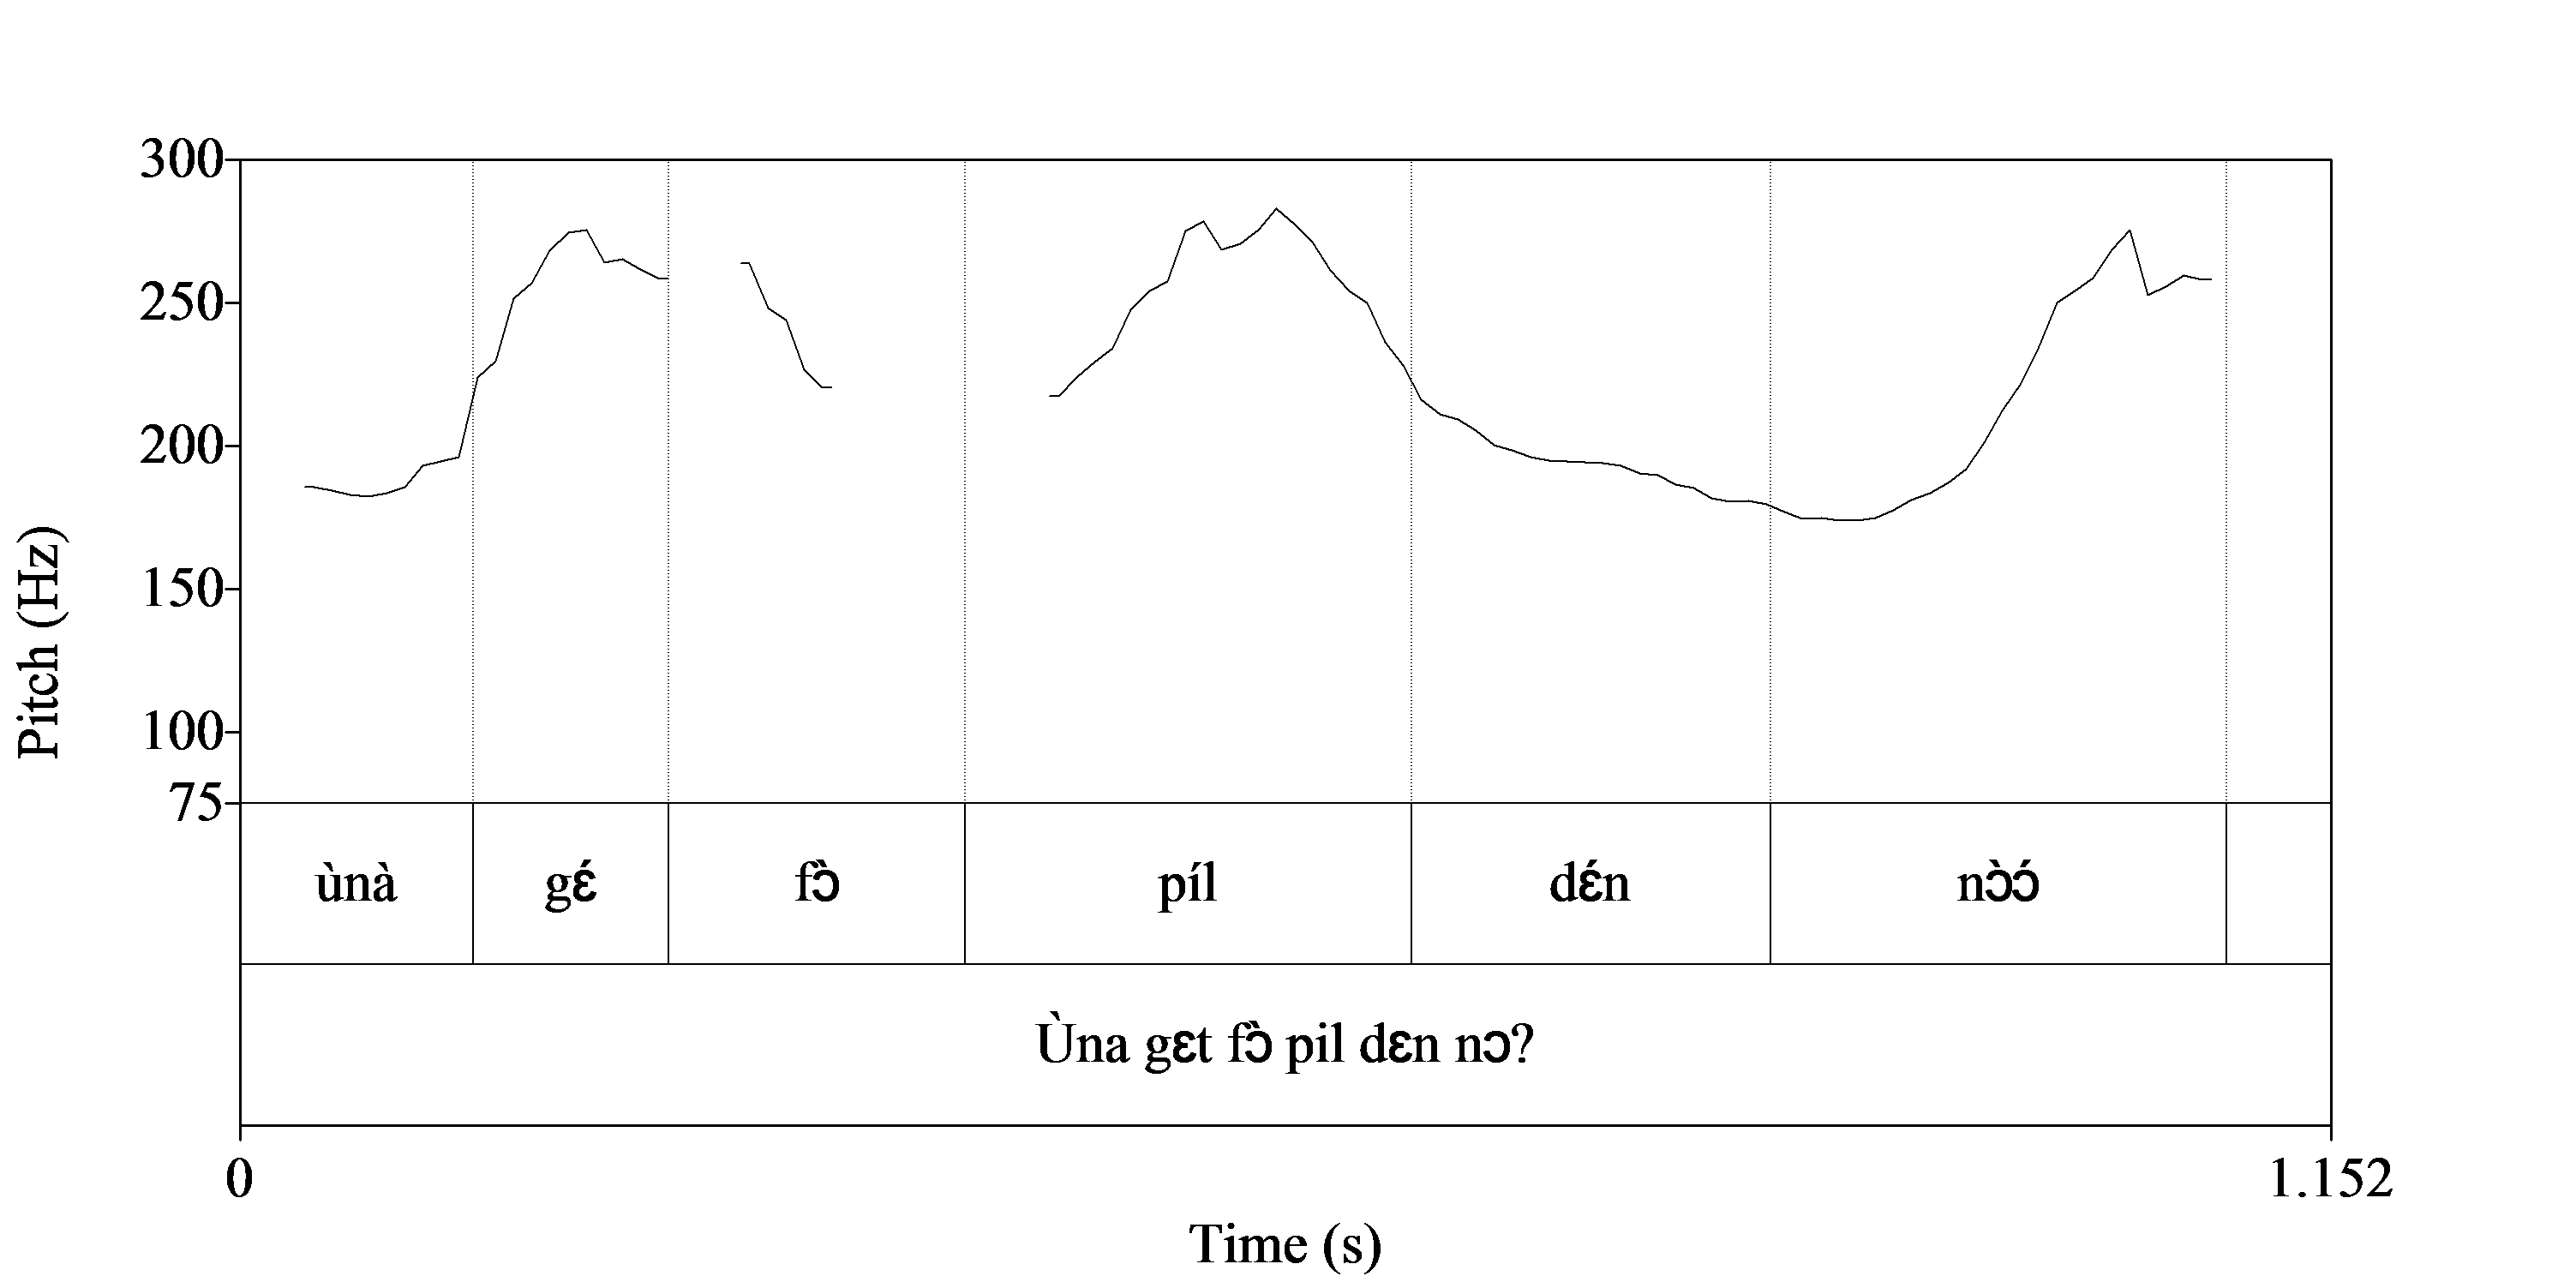
\includegraphics[height=.3\textheight]{figures/yakpomod-img46.png}
\end{figure}

  
 


\ea%97
    \label{ex:key:97}
    \glll   Una    gɛ́fɔ    píl    dɛ́n    nɔ́?\\
\textsc{l.l}    \textsc{h.l}    \textsc{h}    \textsc{l}    \textbf{\textsc{l+h\%}}\\
\textsc{2pl}    have.to  peel    \textsc{3pl.indp}  right\\
\glt ‘You [\textsc{pl}] have to peel them, right [you should know that]?’
\z



The utterance-final syllable in the question above exhibits a particularly steep rise. At the same time, emphasis\is{emphasis} is additionally expressed through pitch range expansion. The contrast between H and L tones is widened across the entire utterance as can be seen by the deep troughs in the pitch trace.\is{question intonation}

 
% \chapter{Morphology}

Pichi nouns and verbs constitute two major word classes. Adjectives, prepositions, and adverbs constitute minor word classes with a few members each. Pichi word formation strategies are predominantly analytic. Besides that, the use of one (adverb-deriving) affix and morphological tone play a role in Pichi derivation and inflection.

\section{Word classes}\label{sec:4.1}

Pichi word classes are differentiated by their syntactic functions (e.g. a noun may head an \textsc{NP}), distribution within the sentence (e.g. a preposition may not be preceded by an article), the morphosyntactic categories that may be specified for them (e.g. verbs may be specified for tense\is{tense}, \isi{aspect}, and \isi{modality}), their derivational potential (e.g. personal pronouns and prepositions are not normally reduplicated, and adverbs do not function as nouns), as well as semantic criteria (dynamic states-of-affairs and property concepts are generally expressed as verbs). 


The major underived word classes, with the most members and the potential to occur in the largest range of environments, are nouns and verbs. The noun-verb distinction in Pichi is quite strong: although verbs may function as nouns in specific (e.g. in emphatic) contexts, the reverse is not usually the case. The verb-adjective distinction is weak. There are only a handful of adjectives, which are indistinguishable from verbs in most environments. The minor word classes consist of adjectives, prepositions, adverbs, as well as various sentence elements that contribute to the meaning of the sentence. 


\subsection{Nominals}

Nouns appear as one of up to three core participant\is{core participants}s of a verb, i.e. as subjects or up to two objects\is{objects}. Nouns also occur as objects of prepositions, and they may function as adverbials. They may be modified by other elements of the noun phrase (e.g. \textit{di} ‘\textsc{def}’, \textit{dá(n)} ‘that’, \textit{sɔn} ‘some, a’ or \textit{dɛn} ‘\textsc{pl’)}, including other nouns in associative constructions and compounds. \is{associative constructions}The vast majority of nouns bears a single H tone and belongs to one of the major tone classes (cf. \tabref{tab:key:3.2}). Underived nouns typically denote time-stable object concepts. Nouns also belong to an open class which may be extended by compounding, conversion, and borrowing\is{borrowing} from \ili{Spanish}.


Personal pronouns, pronominals, and compound question word{\fff}s are subsets of nominals that exhibit a more restricted distribution. Personal pronouns are found in the same syntactic positions as noun phrases but do not cooccur with preposed modifiers. The latter usually also holds true for the pronominals \textit{nátin} ‘nothing’, \textit{sɛ́f} ‘self’, and \textit{yón} ‘own’. The pronominals \textit{káyn} ‘kind’ and \textit{wán} ‘one’ have a wider distribution but are also characterised by specific syntactic preferences. Locative nouns{\fff} form a further subclass of nominals characterised by distributional specificities. Locative nouns are not often preceded by modifiers or determiners, and their distribution overlaps with that of prepositions. 


\subsection{Verbs and adjectives}\label{sec:4.1.2}

Verbs occupy the centre of the predicate. The predicate is best seen to include a number of functional elements that form a tightly-knit unit with the verb in order to constitute clauses: TMA markers, preverbal adverbs\is{preverbal adverbs}, the negator, dependent personal pronouns, as well as the clitic \textsc{3sg} object pronoun. Verbs are usually preceded by a subject noun, pronoun, or both. Verbs may optionally be followed by objects\is{objects}. They are typically mono- or bisyllabic and usually belong to one of the three major tone classes. 


There are numerous subclasses of verbs which can be defined along formal and semantic lines: Aspectual and modal verbs, transfer and communication verbs, stative, inchoative-stative, and dynamic verbs, labile verbs{\fff}, and copula verbs. Other than reduplication, Pichi only has marginally productive means of verb derivation through compounding{\fff}. There are numerous other strategies for the creation of new verbal meanings, e.g. light verb constructions, involving \textit{gɛ́t} ‘get, have’, \textit{mék} ‘make’, or \textit{gí} ‘give’, as well as systematic borrowing{\fff} from Spanish.



There is just a handful of adjectives in Pichi. A small set of property items alternates between uses as inchoative-stative verbs and as adjectives (cf. \tabref{tab:key:7.11} in \sectref{sec:7.6.5}). {\fff}The overwhelming majority of property concepts are lexicalised as inchoative-stative verbs in Pichi. The following “semantic types” \citep[3]{dixon_adjective_2004} are expressed through inchoative-stative verbs: Dimension (e.g. \textit{bíg} ‘be big’, \textit{smɔ́l} ‘be small’, and \textit{lɔ́n} ‘be long’), age (e.g. \textit{ól} ‘be old’ and \textit{yún} ‘be young’), value (e.g. \textit{bád} ‘be bad’, \textit{fáyn} ‘be good’, and \textit{trú} ‘be true’), and colour (e.g. \textit{blák} ‘be black’, \textit{wáyt} ‘be white’, \textit{rɛ́d} ‘be red’, and \textit{yɛ́lo} ‘be yellow’). Most physical properties are also lexicalised as inchoative-stative verbs (e.g. \textit{hád} ‘be hard’, \textit{sáf} ‘be soft’, \textit{sók} ‘be wet’, \textit{évi} ‘be heavy’, \textit{hɔ́t} ‘be hot’, \textit{swít} ‘be tasty’). 



Human propensities are divided between inchoative-stative (e.g. \textit{gudhát} ‘be good-hearted’, \textit{wíkɛd} ‘be wicked’, \textit{badhát} ‘be mean’, \textit{klɛ́va} ‘be clever’) and dynamic verbs (e.g. \textit{gládin} ‘be glad’, \textit{jɛ́lɔs} ‘be envious’) according to whether they denote intrinsic or transient properties. Resultatives{\fff} are exclusively expressed through the stative readings of labile change-of-state verbs (e.g. \textit{brók} ‘break, be broken’, \textit{chɛ́r} ‘tear, be torn’, \textit{lɔ́s} ‘lose, be lost’ and \textit{wɛ́r} ‘be dressed’). Semantic types like position or location are expressed through other means, such as copula clauses featuring the locative-existential copula \textit{dé} (cf. e.g. \ref{ex:key:793}–\ref{ex:key:794}) in combination with adverbials, or through locative verbs like {\fff}\textit{lé} ‘lie’ and \textit{tínap} ‘stand (up)’ (cf. \sectref{sec:8.1.3}).


\subsection{Other word classes}\label{sec:4.1.3}

Most prepositions must be followed by an object, although some may be stranded\is{stranding}, that is, they may occur in the clause-final position. Prepositional phrases are found in the clause-initial or -final position. A majority of prepositions is monosyllabic, a few are bisyllabic. Pichi exhibits a division of labour between prepositions, locative nouns, locative adverbs, and locative verbs in order to express spatial relations. The language has a small number of underived adverbs, amongst them a group of four preverbal adverbs\is{preverbal adverbs}.


Each of the following groups of modifiers may also be said to constitute minor word classes unto themselves, because they occupy distinct syntactic positions in the noun phrase or predicate: the article, demonstratives, quantifiers, prenominal attributive modifiers, numerals, the pluraliser\is{pluraliser}, emphasis markers, topicalisers, TMA markers, aspectual and modal verbs, the general negator, interjections, and ideophones\is{ideophones}. Certain elements modify sentences in their entirety with respect to pragmatic status (e.g. question words, tags, focus particles, interjections) or link sentences with each other (e.g. clause linkers and conjunctions). These sentential elements may also each be considered a separate word class due to their functions and syntactic behaviour.\is{word classes} 


\section{Inflection}\label{sec:4.2}

Most grammatical functions are realised analytically by independent words without the morphological modification of heads or dependents. Participant-marking is taken care of by prepositions and locative nouns, serial verb constructions, and word order, and nominal modification by juxtaposition of adjectives and other modifiers\is{word orderes}. Number-marking is achieved by post-nominal modification. 

The verbal category of number is signalled by personal pronouns and reduplication. Complementisers, preverbal TMA markers, serial verb constructions, and adverbs participate in expressing the grammatical categories of tense{\fff}, modality, and aspect. Comparison is expressed by adverbs of degree, ideophones, verbs, phrasal expressions, suprasegmental modification, serial verb constructions, and prepositions. There are, however, exceedingly rare cases of number marking on \textit{gɛ́l/gál} ‘girl’ and \textit{bɔ́y} ‘boy’ by an apparently marginal plural affix \{-s\}, hence \textit{gɛ́l-s}, \textit{bɔ́y-s}. 


A description of the only inflectional morphological processes follows. The expression of the grammatical relations of subject, object, and possessive case may be seen to involve the use of (tonal) suprafixation, summed up in \tabref{tab:key:4.1} (cf. \sectref{sec:5.4.1} for the full pronominal paradigm and examples).


%%please move \begin{table} just above \begin{tabular
\begin{table}
\caption{Suprafixation with personal pronouns}
\label{tab:key:4.1}

\begin{tabularx}{.75\textwidth}{Xl}
\lsptoprule

Category expressed & Suprafix\\
\midrule
Object case \& independent pronouns & H tone\\
Subject \& possessive case & L tone\\
\lspbottomrule
\end{tabularx}
\end{table}

Tone-conditioned suppletive allomorphy also fulfils inflectional functions in Pichi, even if it involves outright substitution rather than morphological modification (cf. \sectref{sec:3.3}). It has been suggested that the cognate form of the Pichi imperfective marker \textit{de} ‘\textsc{ipfv}’ be analysed as an inflectional verbal prefix in Jamaican Creole \citep[30]{Farquharson2007}. In Pichi too, the use of resumptive imperfective marking with the preverbal aspectual adverbs \textit{jís/jɔ́s} ‘just’ and \textit{stíl} ‘still’ suggests a tighter-than-usual syntagmatic relation between the imperfective aspect marker and the verb it modifies:


\ea%98
    \label{ex:key:98}
    \gll   Náw    dɛn  \textbf{de}  \textbf{jís}  \textbf{de}  kán.\\
now    \textsc{3pl}  \textsc{ipfv}  just  \textsc{ipfv}  come\\

\glt ‘Now, they’re just coming.’ [ye07je 179] \is{preverbal adverbs}
\z

\section{Derivation}\label{sec:4.3}

Pichi makes use of morphological processes for the purpose of derivation. One is a tonal process which derives compounds, including reduplications. The other is adverb-deriving suffixation. Compounding and reduplication are two highly productive derivational processes in Pichi. 

\subsection{Affixation}
\tabref{tab:key:4.2} summarises the derivational processes found in Pichi. This section covers formal aspects of compounding and reduplication, which both receive a more detailed functional treatment in \sectref{sec:4.4} and \sectref{sec:4.5.1}, respectively. Adverb-deriving suffixation is covered in this section in both its formal and functional aspects.

%%please move \begin{table} just above \begin{tabular
\begin{table}
\caption	{Derivational processes}
\label{tab:key:4.2}
{\small\begin{tabularx}{\textwidth}{QQ lQ l}
\lsptoprule
Category expressed & Word class applied to & (Supr-)affix & Process & Productivity\\
\midrule
Verbal plurality & Dynamic verbs & L tone + \textsc{red} & Tone deletion + iteration & High\\

\tablevspace
Nominal and verbal compound & Nouns, pronouns verbs, adverbs, phrases & L tone & Tone deletion & Fair\\

\tablevspace
Manner adverb & Verbs, adjectives & {}-\textstyleTablePichiZchn{wán} \textsc{‘adv’} & Suffixation & Low\\
\lspbottomrule
\end{tabularx}}
\end{table}

Compounding and reduplication both make use of the same tonal derivation. Reduplication is therefore best seen as a form of (self-)compounding in Pichi. In the process, the H tone over the initial component(s) is deleted and replaced by an L tone. The final component retains its original tone configuration. The resulting compound word then features a single H tone like most Pichi words. Pichi compounds are therefore right-headed; the L-toned initial component(s) function as modifier(s) to the final component, which is the head. 


Nouns, verbs, adjectives, and adverbs participate in compounds. The resulting structures may function as nouns or verbs. Personal pronouns may also participate as modifiers in compound personal pronouns (cf. \sectref{sec:5.4.2}). Compounding is fairly productive (cf. \sectref{sec:4.4} for details). Compare the compound in \REF{ex:key:99} featuring the modifier noun \textit{kɔ́ntri} ‘country, home town’ and the modified noun \textit{chɔ́p} ‘food’. While \textit{kɔ́ntri} loses the H tone over its first syllable, the head noun \textit{chɔ́p} retains its original H tone:



\ea%99
    \label{ex:key:99}
    \gll   Na  in    \textbf{kɔntri}{}-\textbf{chɔ́p}.\\
\textsc{foc}  \textsc{3sg.poss}  country.\textsc{cpd}{}-food\\

\glt ‘That’s his local food.’ [au07ec 007]
\z

Compounding through tone deletion also characterises the reduplication of dynamic verbs in order to derive verbal number \REF{ex:key:100}. This kind of derivation is fully productive for all dynamic verbs. Equally, it can be observed with a small number of lexicalised reduplications involving other word classes (cf. \sectref{sec:4.5.3}):


\ea%100
    \label{ex:key:100}
    \gll Kán  tót    bɛlɛ́,    bigín  de  \textbf{hala}-\textbf{hála}  náw,  \textbf{hala}-\textbf{hála}.\\
\textsc{pfv}  carry  belly  begin  \textsc{ipfv}  \textsc{red.cpd-}shout  now    \textsc{red.cpd-}shout\\

\glt ‘(Then she) became pregnant, (and) began lamenting and lamenting.’ [ab03ay 118]\is{derivation:tonal}
\z

Adverbs are derived from verbs and adjectives by means of the suffix -\textit{wán} \textsc{‘adv’}, etymologically related to the numeral \textit{wán} ‘one’. Amongst its numerous other uses (cf. \sectref{sec:5.3.1}), the cardinal numeral \textit{wán} ‘one’ serves as a pronominal substitute for nouns in \textsc{NPs} featuring attributively used property items (i.e. \textit{di blák wán} ‘the black one’; \textit{di bíg wán} ‘the big one’). When such \textsc{NPs} appear in an adverbial slot in the clause, the resulting structure functions as a manner adverb. 


The semantic link between the function of -\textit{wán} \textsc{‘adv’} as an adverbialising suffix and the meaning of \textit{wán} in other contexts is opaque. This warrants the analysis of -\textit{wán} ‘\textsc{adv’} as a suffix rather than seeing it as the second component of a compound word. \is{derivation:affixation}The derivation of adverbs is a derivational process distinct from compounding and does not involve the tone deletion that accompanies the latter kind of word formation. In the following examples, the property items \textit{fáyn} ‘(be) fine’ \REF{ex:key:101} and \textit{smɔ́l} ‘(be) small’ \REF{ex:key:102} and the affix \textit{-wán} retain their lexically assigned H tone. The resulting adverbs are bisyllabic, bimorphemic words with an H\textsc{{}-}H (downstepped H) tone configuration:\is{cardinal numerals}



\ea%101
    \label{ex:key:101}
    \gll E    mék=an    \textbf{fáyn-wán}.\\
\textsc{3sg.sbj}  make=\textsc{3sg.obj}  fine\textsc{{}-adv}\\

\glt ‘She made it nicely.’ [ra07ve 017]
\z


\ea%102
    \label{ex:key:102}
    \gll E    fáyn    fɔ  dríng  \textbf{smɔ́l-wán}.\\
\textsc{3sg.sbj}  fine    \textsc{prep}  drink  small\textsc{{}-adv}\\

\glt ‘It’s good to drink moderately.’ [ma03hm 071]
\z

The derivation of manner adverbials through the suffixation of -\textit{wán} is not particularly productive. In the corpus, it is unanimously accepted with a limited number of monosyllabic property items denoting physical properties, such as \textit{smɔ́l} ‘be small’, \textit{kól} ‘be cold’, \textit{hɔ́t} ‘be hot’, \textit{fáyn} ‘be fine’. In contrast, the formation of adverbials with many other property items was rejected by informants, amongst them \textit{dɔtí} ‘be dirty’, \textit{bád} ‘be bad’, \textit{bɛlfúl} ‘be satiated’, \textit{nékɛd} ‘be naked’, \textit{táya} ‘be tired’, \textit{lét} ‘be late’, \textit{frɛ́s} ‘be fresh’, \textit{rɛ́p} ‘be ripe’, and \textit{sáful} ‘be slow, diligent’. 


The generic noun \textit{tɛ́n} occurs in a small number of more or less lexicalised expressions functioning as sentence and time adverbs. All of the expressions contained in the corpus are listed in \REF{ex:key:103}. Like derived adverbs featuring the suffix -\textit{wán} ‘\textsc{adv}’, these bisyllabic expressions are not compounds, since there is no tonal derivation. 



\is{cardinal numerals}The meanings of these expressions are semantically distinct from the meanings of their components in varying degrees. The degree of semantic opaqueness of each collocation is reflected in the orthographic choice of writing them as single or separate words. A good indicator of the  degree of semantic unity of the collocations in \REF{ex:key:103} is their behaviour during repetition\is{repetition} for emphasis (cf. \ref{ex:key:152} further below). Even in the lexicalised expressions (e.g. \textit{bádtɛn} ‘unfortunately) each morpheme nevertheless retains its original pitch, as shown by tone marking. This renders complex words with a sequence of two H tones (the second H undergoes downstep).

\eabox{\label{ex:key:103}
\begin{tabularx}{.9\textwidth}{lll}
Construction & Components & Gloss\\
\itshape lɔ́n tɛ́n & long time & ‘long time ago’\\
\itshape (di) fɔ́s tɛ́n & (the) first time & ‘(the) first time, formerly’\\
\itshape wán tɛ́n & one time & ‘once’\\
\itshape wán.tɛn & one.time & ‘at once, suddenly’\\
\itshape bád.tɛn & bad.time & ‘unfortunately’\\
\itshape smɔ́l.tɛn & small.time & ‘shortly, nearly’ \\
\itshape sɔn tɛ́n dɛn & some time \textsc{pl} & ‘sometimes’\\
\itshape sɔn.tɛ́n & some.time & ‘perhaps’\\
\end{tabularx}
}
The largely unpredictable meanings of the adverbs in \REF{ex:key:103} are reason enough to consider them as lexicalised phrasal expressions, rather than analysing \textit{tɛ́n} as a productive adverbialising suffix. 

\subsection{Conversion}

Some word classes\is{word classes} are characterised by multifunctionality. They may undergo conversion and appear in a syntactic position reserved for another class without morphological derivation. \tabref{tab:key:4.3} provides an overview of productive conversion. Some processes are unidirectional, others bidirectional. Arrows indicate the direction of conversion\textstyleannotationreference{.} The productivity of conversion varies with word class and is often subject to lexical idiosyncracies. 

%%please move \begin{table} just above \begin{tabular
\begin{table}
\caption{Conversion}
\label{tab:key:4.3}

{\small\begin{tabularx}{\textwidth}{llcl}
\lsptoprule

Type of conversion & Word class & Direction & Word class\\
\midrule
Change in & Verb & \phantom{←  }→ & Noun\\
word class & Predicate adjective & \phantom{←  }→ & \textit{\textup{Verb}}\\
& \textit{\textup{Verb (property concept)}} & ←  → & Attributive adjective\\
& Noun & \phantom{←  }→ & \textit{\textup{Adverbial}}\\

\tablevspace
No change in & Inchoative-stative verb & ←  → & Dynamic verb\\
word class & Noun & ←  → & Modifier noun\\
\lspbottomrule
\end{tabularx}}
\end{table}

Verbs may be employed in the syntactic position of nouns. This process of conversion is very productive. The meanings of such nominalised verbs vary in accordance with their lexical aspect. A dynamic verb used as a noun denotes the nominalised activity, while an (inchoative-)stative verb used in such a way denotes the corresponding nominalised state. 


In \REF{ex:key:104}, the dynamic verb \textit{hála} ‘shout’ is used as a dynamic noun or “action nominal”, (\citealt{ComrieThompson1985}). In \REF{ex:key:105}, the inchoative-stative verb \textit{gúd} ‘be good’ is employed as a stative noun or “state nominal” (\citealt{ComrieThompson1985}). The use of nominalised verbs as cognate objects \is{cognate objects}is common for emphasis (cf. \sectref{sec:9.3.3}). Cognate objects\is{objects} behave no differently from other nominalised verbs:



\ea%104
    \label{ex:key:104}
    \gll E    sé    frɔn    \textbf{dán}    \textbf{hála}    dí  pikín  nó  slíp    mɔ́.\\
\textsc{3sg.sbj}  \textsc{quot}    from  that    shout  this  child  \textsc{neg}  sleep  again\\

\glt ‘She said from that shout(ing) onwards this child didn’t sleep anymore.’ [ab03ab 075]
\z


\ea%105
    \label{ex:key:105}
    \gll \'{A}fta    ínsay  \textbf{dán}    \textbf{gúd}    wé  a    trata  yú    na  dé
mi    mán    go  chɛ́k  sé    mi    rabia  dɔ́n  fínis.\\
then  inside  that    good  \textsc{sub}  \textsc{1sg.sbj}  treat  \textsc{2sg.indp}  \textsc{foc}  there
\textsc{1sg.poss}  man    \textsc{pot}  think  \textsc{quot}    \textsc{1sg.poss}  anger  \textsc{prf}  finish\\
\glt ‘Then through that goodness that I treated you with, that’s where my 
husband would think that my anger has finished.’ [ro05rr 003]
\z

A verb can also appear in the nominal position together with its object, although this is rarely heard in natural speech: 


\ea%106
    \label{ex:key:106}
    \gll Na  \textbf{di}  \textbf{wás}    \textbf{klós},  na  di  tín    mék    yu  táya.\\
\textsc{foc}  \textsc{def}  wash  clothing  \textsc{foc}  \textsc{def}  thing  make  \textsc{2sg}  be.tired\\

\glt ‘It’s the washing of clothing, that’s why you’re tired.’ [dj05be 039]
\z

In contrast, very few nouns are attested in the syntactic position of verbs. The noun \textit{bɛlɛ́} ‘belly’ \REF{ex:key:107} may be used as a verb with the meaning ‘impregnate’ \REF{ex:key:108}. Other noun-verb pairs in the corpus that may be employed in a similar way are \textit{kaká} ‘defecate, faeces’, \textit{pipí} ‘urinate, urine’, \textit{rút} ‘root, uproot’, \textit{latrín} ‘toilet, go to toilet’. These rare cases are not listed in \tabref{tab:key:4.3} because they are lexicalised, and there is hence no productive noun-verb conversion. 


\ea%107
    \label{ex:key:107}
    \gll Tidé    pikín,  yu  go  gɛ́t  \textbf{bɛlɛ́}    yu  púl=an
yu  go  dáy  wet    \textbf{bɛlɛ́}.\\
today  child  \textsc{2sg}  \textsc{pot}  get  belly  \textsc{2sg}  remove=\textsc{3sg.obj}
\textsc{2sg}  \textsc{pot}  die  with    belly\\

\glt ‘(As for) children of today, you could get pregnant and remove it 
and you could die due to pregnancy.’ [ab03ay 105]
\z


\ea%108
    \label{ex:key:108}
    \gll A    fía  sé    dɛn  go  \textbf{bɛlɛ́}      mi    pikín  fɔ  mí.\\
  \textsc{1sg.sbj}  fear  \textsc{quot}    \textsc{3pl}  \textsc{pot}  impregnate  \textsc{1sg.poss}  child  \textsc{prep}  \textsc{1sg.indp}\\
\glt ‘I feared that they could impregnate me my child.’ [dj05be 055]\is{derivation:conversion}
\z

Other word class\is{word classes}es are also characterised by multifunctionality. Members of the small adjective class of Pichi may be used as inchoative-stative verbs without a change in form (cf. \sectref{sec:7.6.5}). Property items, whether adjectives or verbs, may be employed as attributive adjectives (i.e. prenominal modifiers, cf. \sectref{sec:5.2.1}), and nouns may modify other nouns in associative constructions without an overt process of derivation (cf. \sectref{sec:4.4.2}). Further, labile verbs\is{labile verbs} may be used in their respective lexical aspect classes without any formal change (cf. \sectref{sec:9.2.3}). Such multifunctionality with respect to lexical aspect class is very productive. It is lexically restricted to the class of labile verbs, which constitutes a large verb class in Pichi. Aside from that, members of the small class of adverbs are not usually employed as nouns or verbs.\is{conversion} 

\section{Compounding}\label{sec:4.4}

Pichi makes extensive use of compounding in order to derive nouns, verbs, and personal pronouns. Compound words are formed by combining two, sometimes more lexical items. Most types of compounding are covered in \sectref{sec:4.4}. Reduplication, which also involves compounding, is covered separately in section \sectref{sec:4.5.1}. Aspects of the morphophonology of compounding are covered in \sectref{sec:3.2.4}.\is{derivation}

\subsection{General characteristics}

Compounding forms part of a continuum of possessive constructions or relations of modification between constituents (cf. also \sectref{sec:5.2.3}). I only refer to those possessive constructions as “compounds” which form single phonological words via the tonal derivation described in \sectref{sec:3.2.4}. I nevertheless use the term “compounding” as a generic term to designate the formative processes that derive compounds associative constructions and \textit{fɔ}{}-constructions. Compounds relate in interesting ways to associative constructions and \textit{fɔ}{}-prepositional phrase constructions. The two latter types of possessive constructions are formed by syntactic concatenation alone. In the following, I refer to the individual lexical items occurring in these three types of possessive constructions as “components”. \tabref{tab:key:4.4} provides an overview of relevant characteristics of the three types of compounding: 

%%please move \begin{table} just above \begin{tabular
\begin{table}
\caption{Characteristics of compounding}
\label{tab:key:4.4}
\fittable{
\begin{tabular}{llll}
\lsptoprule
Features & Compounds & Associative constructions & \textit{Fɔ}{}-construction\\
\midrule
Morphosyntax & Tonal derivation & Syntactic concatenation & Syntactic concatenation\\
Productivity & Medium & Medium & High \\
Lexicalisation & High & Medium & Low\\
\lspbottomrule
\end{tabular}
}
\end{table}

Phonological and semantic factors determine the choice between compounding and the use of associative constructions for word formation. Speakers may opt to use a compound when the relevant concepts are commonly associated with each other, and the entire structure is conventionalised or lexicalised. In contemporary Pichi, there is no formal difference between compounds that may have been carried over from English (e.g. \textit{pan-kék} ‘pancake’, \textit{ren-sísin} ‘rain(y) season’) and language-internal formations (e.g. \textit{kɔntri-chɔ́p} ‘local food’). The meanings of both groups may be more compositional or more idiosyncratic, and both undergo the same tonal derivation characteristic of compounding:

\eabox{\label{ex:key:109}
\begin{tabularx}{.9\textwidth}{XXX} 
         Compound & Components & Gloss\\
\itshape kɔntri-chɔ́p & country-food & ‘local food’\\
\itshape kichin-písis & kitchen-cloth & ‘kitchen rag’\\
\itshape waka-stík & walk-stick & ‘walking stick’\\
\itshape ren-sísin & rain-season & ‘rainy season’\\
\itshape pan-kék & \textit{\textup{pan-cake}} & ‘pancake’\\ 
\end{tabularx}
}

Some semantically opaque compounds also exist, in which one component has no independent meaning (\ref{ex:key:110}a) or where one component is obsolete (b). It is noteworthy that the initial components of the first two compounds below exhibit a regular sound-meaning relation with the verbs \textit{spót} ‘be stylish’ and \textit{lúk} ‘look’, respectively, although there is no nominalising suffix \textit{*-in} in Pichi. However, there is one verb-noun pair in the corpus, in which the noun (\textit{bɛ́rin} ‘burial’) is the action nominal to a verb (\textit{bɛ́r} ‘bury’). The compound in (c) is therefore transparent and fully segmentable. Opaque and exocentric compounds are written without a hyphen in this work and their components are separated by a dot where relevant: 

\eabox{\label{ex:key:110}
\begin{tabularx}{.9\textwidth}{lXXX}
   & Compound & Components & Gloss\\
a. & \itshape spotin.bɔ́y & \textstyleTablePichiZchn{*spotin}.boy & ‘stylish guy’\\
   & \itshape lukin.glás & \textstyleTablePichiZchn{*lukin}.glass & ‘mirror’\\
   & \itshape kobo.fút & \textstyleTablePichiZchn{*kobo}.foot & ‘bowlegs’\\
\tablevspace   
b. & \itshape faya-wúd & \itshape \textup{fire}{}-?wúd & ‘firewood’\\
\tablevspace   
c. & \itshape bɛrin-grɔ́n & burial-ground & ‘burial ground’\\
\end{tabularx}
}

Other collocations are also partially opaque but exhibit the prosodic characteristics of either associative constructions or compounds. These are  structures that have inherited varying degrees of semantic opacity and lexicalisation from English, cf. (\ref{ex:key:111}–\ref{ex:key:113}). In the compounds in \REF{ex:key:111}, both components before and after the dot retain their original pitch configurations. In collocations involving the generic noun \textit{dé} ‘day’ as a modified noun, the “modifier” has no meaning of its own:

\eabox{\label{ex:key:111}
\begin{tabularx}{.9\textwidth}{XXX}
Compound & Components & Gloss\\
\itshape hɔ́li.dé & *\textstyleTablePichiZchn{hɔ́li}.\textstyleTableEnglishZchn{day} & ‘holiday’\\
\itshape yɛ́sta.dé & *\textit{yɛ́sta}.day & ‘yesterday’\\
\itshape sáti.dé & *\textstyleTablePichiZchn{sáti}.\textstyleTableEnglishZchn{day} & ‘Saturday’\\
\end{tabularx}
}
The structure of two sets of kinship terms is also of interest. The root \textit{gran-} ‘grand-’ is segmentable and has a discernible meaning. However, the root is never found independently of the word it modifies. It only appears in compounds (\ref{ex:key:112}a), which can, in turn, be preceded by the prenominal modifier \textit{grét} ‘great’ (b):

\eabox{\label{ex:key:112}
\begin{tabularx}{.9\textwidth}{lXXX}
         & Compound & Components & Gloss\\
a. & \itshape gran-mɔ́da & grand-mother & ‘grandmother’\\
& \itshape gran-má,~gran-mamá & grand-ma/-mother & ‘grandma/grandmother’\\
& \itshape gran-pá, gran-papá & grand-pa/-father & ‘grandpa/grandfather’\\
& \itshape gran-pikín & grand-child & ‘grandchild’\\
b. & \itshape grét gran-pikín & great grand-child & ‘great grandchild’\\
\end{tabularx}
}

The second set of kinship-denoting compounds contains the segmentable root \textit{lɔ́} ‘law’ as the final component. The composite meanings of these compounds are idiosyncratic. Additionally, some of the structures are fully segmentable, with the first component constituting an independent word (\ref{ex:key:113}a). Further, we find variants of group (a) compounds with slightly altered initial components (b). With these, the etymology is clear, but the altered initial component never occurs on its own. A final group contains an opaque initial element, which is a fossilised English morpheme that does not exist (any longer) in contemporary Pichi (c): 

\eabox{\label{ex:key:113}
\begin{tabularx}{.9\textwidth}{lXXX}
         & Compound & Components & Gloss\\
a. & \itshape mɔda-lɔ́ & mother-law & ‘mother-in-law’\\
& \itshape fada-lɔ́ & father-law & ‘father-in-law’\\
& \itshape brɔda-lɔ́ & brother-law & ‘brother-in-law’\\
& \itshape sista-lɔ́ & sister-law & ‘sister-in-law’\\
b. & \itshape mɔdɛ-lɔ́ & \textstyleTablePichiZchn{*mɔdɛ}.law & ‘mother-in-law’\\
& \itshape sistɛ-lɔ́ & \textstyleTablePichiZchn{*sistɛ}.law & ‘sister-in-law’\is{kinship terminology}\\
c. & \itshape dɔta.lɔ́ & \textstyleTablePichiZchn{*dɔta}.law & ‘daughter-in-law’\\
& \itshape sɔni.lɔ́ & \textstyleTablePichiZchn{*sɔni}.law & ‘son-in-law’\\
\end{tabularx}
}
In Spanish compounds and neologisms involving Spanish components (e.g. \textit{busca-blanco} ‘female sex worker specialised to white men’), the initial component(s) is/are always low-toned, while the final component bears H tone on the penultimate or only syllable \REF{ex:key:114}. This also holds for reduplicative compounds involving Spanish-derived dynamic verbs. The H tone is therefore found on the syllable that is stressed in standard Spanish. However, when these Spanish-derived compounds are employed in Pichi clauses, the H tone over the final component may not be shifted to other components of the compound for focus or emphasis (as the placement of stress may be in Spanish). This speaks for an analyisis of these collocations as Pichi-style compounds featuring the tonal derivation that other compounds have:

\eabox{\label{ex:key:114}
\begin{tabularx}{.9\textwidth}{lXlX}
Compound & Transcription & Components & Translation\\
\itshape vídeo-club & [vìdjò klúb] & video-club & {‘video\newline rental shop’}\\
\itshape busca-blanco & [bùskà-blánkò] & search-white.male & {‘female sex\newline worker spe-\newline cialised to \newline white men’}\\
\itshape tres mil & [trɛ̀s míl] & three thousand & {‘three thou-\newline sand’}\\
\itshape cuarenta y siete & {[kwàrɛ̀nta ì\newline sjétè]} & forty and seven & ‘forty-seven’\\
\itshape cruza-cruza & [krùsà-krúsà] & cross-cross & ‘cross repeatedly’\\
\end{tabularx}
}
Although in many cases conventionalisation is a good indicator for the use of compounding, phonology may override semantics. Compounds are shunned in favour of associative constructions where the first component belongs to the L.H tone class featuring a word-final H tone. We have seen that this tone class remains unaffected by other tonal and intonational processes as well (cf. e.g. \sectref{sec:3.4.1}). Hence the concepts in \REF{ex:key:115}, although conventionalised, are expressed as associative constructions, syntactic phrases consisting of prosodically independent components:

\eabox{\label{ex:key:115}
\begin{tabularx}{.9\textwidth}{lllX}
Ass. construction & Components & Gloss\\
\itshape bangá súp & palm-nut soup & ‘palm-nut soup’\\
\itshape dɔtí pán & dirt pan & ‘dustbin’\\
\itshape plantí fufú & plantain fufu & ‘fufu made from plantain’\\
\end{tabularx}
}
The tonal derivation characteristic of compounding also distinguishes lexicalised compound verbs (\ref{ex:key:116}a) from verb-object phrases (b) (cf. also \sectref{sec:4.4.3}):

\eabox{\label{ex:key:116}
\begin{tabularx}{.9\textwidth}{lllX}
         & Construction & Components & Gloss\\
a. & \itshape e opin.yáy & \textsc{3sg.obj} open.eye & ‘s/he is enlightened, cultivated’\\
b. & \itshape e ópin yáy & \textsc{3sg.sbj} open eye & ‘s/he opened (her) eye(s)’\\
\end{tabularx}
}

\subsection{Compound nouns}\label{sec:4.4.2}

Compound nouns function as nouns in a clause. Their final component is always a noun, while their initial component(s) may be a noun, verb, or an adverb. Compound nouns are the most common type of compound in the corpus. They instantiate a relation of modification, with the first component serving as the modifier and the second as the modified element. 


In a large number of collocations in the corpus, the modified noun is one of the generic nouns\is{generic nouns} listed in \REF{ex:key:117}, which serve other important functions in the language as well (cf. \citealt[252]{Faraclas1996}):


\eabox{\label{ex:key:117}
\begin{tabularx}{.9\textwidth}{llX}
Type & Generic noun & Gloss\\
 Human & \itshape mán & ‘man, person’\\
  & \itshape húman & ‘woman’\\
  & \itshape bɔ́y & ‘boy’\\
  & \itshape gɛ́l & ‘girl’\\
  & \itshape pikín & ‘child, member of group’\\
  & \itshape pɔ́sin & ‘person’\\
  & \itshape pípul & ‘people’\\
 Place & \itshape sáy & ‘side, place’\\
  & \itshape pát & ‘part, place’\\
  & \itshape plés & ‘place’\\
 Manner & \itshape stáyl & ‘style’\\
  & \itshape fásin & ‘manner’\\
 Time & \itshape tɛ́n & ‘time’\\
  & \itshape áwa & ‘hour, time’\\
 Entity & \itshape tín & ‘thing’\\
  & \itshape wán & ‘one’\\
  & \itshape káyn & ‘kind’\\
\end{tabularx}
}
The tendencies of nominal compounding are summarised in \tabref{tab:key:4.5}. The column “modifier/modified” in \tabref{tab:key:4.5} lists the types of modification relations attested in the data. I have added the third relevant possessive construction, the “\textit{fɔ}{}-construction” for comparison. The columns headed by “compound”, “associative construction”, and “\textit{fɔ}{}-construction” contain a cross (x) if the structure is employed to express the corresponding relation in the leftmost column. A blank space indicates that the structure is not employed for this purpose. 

%%please move \begin{table} just above \begin{tabular
\begin{table}
\caption{Tendencies of nominal compounding}
\label{tab:key:4.5}
\fittable{
\begin{tabular}{lccc}
\lsptoprule
Modifier/modified & Compound & \textsc{Ass}ociative construction & \textit{Fɔ}{}-construction\\
\midrule 
Group/member of &  & x & x\\
\tablevspace
Gender of/creature &  & x & \\
\tablevspace
Measure/entity &  & x & \\
\tablevspace
Kind of/entity & x & x & x\\
\tablevspace 
Activity/agent & x &  & \\
\lspbottomrule
\end{tabular}
}
\end{table}
Compounds, associative constructions, and \textit{fɔ}{}-prepositional constructions form part of a continuum of “possessive” constructions. In this continuum, associative constructions may express the widest range of modification relations, including most relations that may also be expressed as compounds and \textit{fɔ}{}-prepositional constructions (cf. also \sectref{sec:5.2.3}). \tabref{tab:key:4.5} shows that compound nouns are only used to express “kind of/entity” relations – the “activity/agent” relation being a subtype of the “kind of/entity” relation in which the first component is a dynamic verb and the second a human-denoting noun.


In turn, associative constructions represent the conventional means of expressing a measurement relation (referred to as “measure\slash entity” in \tabref{tab:key:4.5}), a “group\slash member of” relation featuring the modified noun \textit{pikín} ‘child’, and a “gender of\slash creature” relation featuring the gender nouns \textit{mamá} ‘mother’ and \textit{papá} ‘father’, \textit{mán} ‘man’ and \textit{húman} ‘woman’, or \textit{bɔ́y} ‘boy’ and \textit{gál} ‘girl’ in the modifier position. 



Secondly, associative constructions are the default option for expressing “kind of\slash entity” relations when these are not expressed as compounds. One criterion that determines the use of an associative construction as a default option is the nature of the modifier noun. Modifier nouns with an L.H pitch configuration and/or with more than two syllables are less likely to undergo the tone deletion that derives compound nouns. A second, subsidiary criterion is the lack of conventionalisation or lexicalisation of the collocation. In all other cases, “kind of\slash entity” relations, including “activity\slash agent” relations are usually expressed through compounds. Nevertheless, allowance must be made for numerous lexicalised exceptions to these tendencies.



In “kind of/entity” compounds, the first component modifies the second as to certain qualities. These compounds encompass bicomponental food items and dishes (\ref{ex:key:118}a) and body parts (b), as well as other concepts commonly associated with each other (c). Note that \textit{kaka-rás} ‘arse’ in (b) is a lexicalised compound and an exception to the tendency for collocations featuring an L.H modifier noun to be realised as associative constructions (the other most common exception being \textit{bɛlɛ́} ‘belly’ when used in the modifier position of a compound, cf. \ref{ex:key:124}). Compounds are also employed to form highly conventionalised quantifier compounds which express ordinal numerals{\fff} (d) as well as dual and \textit{ɔ́l} ‘all’ extensions of the pronominal system (e).



In sum, the use of “kind of/entity” compounds therefore reflects the degree of conventionalisation of the linkage between the participating nouns and in that a certain degree of inalienability\is{inalienability}:


\eabox{\label{ex:key:118}
\begin{tabularx}{.9\textwidth}{lXXX}
         & Compound & Components & Gloss\\
a. & \itshape pɛpɛ-súp & pepper-soup & ‘pepper soup’\\
& \itshape bwɛl-plantí & boil-plantain & ‘boiled plantain’\\
& \itshape bit-fufú & beat-fufu & ‘pounded fufu’\\
b. & \itshape finga-nél & finger-nail & ‘finger nail’\\
& \itshape kaka-rás & faeces-arse & ‘arse’\\
c. & \itshape hɔt-watá & hot-water & ‘hot water’\\
& \itshape kol-watá & cold-water & ‘cool water’\\
d. & \itshape nɔmba-tú & number-two & ‘second’\\
& \itshape nɔmba-trí & number-three & ‘third’\\
& \itshape las-nɛ́t & last-night & ‘last night’\\
& \itshape las-mán & last-man & ‘last person’\\
e. & \itshape wi-ɔl-tú & \textsc{1pl}{}-all-two & ‘the two of us’\\
& \itshape dɛn-ɔ́l & \textsc{3pl}{}-all & ‘they all’\\
\end{tabularx}
}
Certain “kind of/entity” relations follow in \REF{ex:key:119} that are expressed through associative constructions rather than compounds. Group (a) features collocations, in which the modifier noun belongs to the L.H tone class. Here we also find some highly conventionalised collocations (b). The words in (c) contain associative constructions that involve trisyllabic modifier nouns from different tone classes. Other concepts are not sufficiently conventionalised or lexicalised to appear in compounds even if they present no formal obstacles (d). Also note the “kind of/entity” relations listed in \REF{ex:key:119}: 

\eabox{\label{ex:key:119}
\begin{tabularx}{.9\textwidth}{l llX}
         & Compound & Components & Gloss\\
a. & \itshape granát pamáyn & groundnut oil & ‘groundnut oil’\\
& \itshape Lubá topé & \textsc{place} palmwine & ‘Palmwine from Luba’\\
b. & \itshape dɔtí pán & dirt pan & ‘dustbin’\\
& \itshape plantí fufú & plantain fufu & ‘fufu made from plantain’\\
c. & \itshape kápinta wók & carpenter work & ‘work of a carpenter’\\
& \itshape wahála húman & trouble woman & ‘female trouble maker’\\
& \itshape aráta hól & rat hole & ‘rat hole’\\
& \itshape dominó stón & domino stone & ‘domino stone’\\
d. & \itshape Ghána mɔní & \textsc{place} money & ‘Ghanaian money’\\
& \itshape Píchi wɔ́d & Pichi word & ‘Pichi word’\\
& \itshape skúl plába & school problem & ‘problems related to school’\\
\end{tabularx}
}
Other “kind of/entity” relations are also expressed through associative constructions, although they do not present any phonotactic or semantic obstacles either. For example, the generic noun \textit{tɛ́n} ‘time’ is only recorded as a modified noun in the associative constructions listed in \REF{ex:key:120}, even though these structures are lexicalised and occur very frequently. Note, however, that other, lexicalised collocations involving \textit{tɛ́n} are not expressed as compounds either (cf. \ref{ex:key:103} above):

\eabox{\label{ex:key:120}
\begin{tabularx}{.9\textwidth}{XXX}
          Compound & Components & Gloss\\
\itshape mɔ́nin tɛ́n & morning time & ‘morning’\\
\itshape sán tɛ́n & sun time & ‘(after)noon’\\
\itshape ívin tɛ́n & evening time & ‘evening’\\
\end{tabularx}
}
Compounds involving \textit{sáy} ‘side, place’ are equally scarce. This noun is only attested as a modified noun in three compounds in the corpus, all of which have partially idiosyncratic meanings (\ref{ex:key:121}a). Other equally conventionalised collocations involving \textit{sáy} are expressed through associative constructions (b) or via \textit{fɔ}{}-prepositional constructions (c):

\eabox{\label{ex:key:121}
\begin{tabularx}{.9\textwidth}{lllX}
         & Compound & Components & Gloss\\
a. & \itshape wok-sáy & work-side & ‘work-place’\\
& \itshape rɔn-sáy & wrong-side & ‘inside out, upside-down, reverse’\\
& \itshape gud-sáy & good-side & ‘the right way round’\\
b. & \itshape ɔ́p sáy & up side & ‘(at the) upper part, up (there)’\\
& \itshape bihɛ́n sáy & behind side & ‘(at the) rear’\\
& \itshape dɔ́n sáy & down side & ‘(at the) lower part, down (there)’\\
c. & \itshape sáy fɔ chɔ́p & place \textsc{prep} eat & ‘eating place, restaurant’\\
& \itshape sáy fɔ wás & place \textsc{prep} wash & ‘place for washing, washhouse’\\
\end{tabularx}
}
“Group/member of” structures feature the human-denoting noun \textit{pikín} ‘child’ in the modified position. The conventional way of expressing this relation is through the associative construction. The modified noun \textit{pikín} may acquire quite an idiosyncratic meaning in the collocations listed under (\ref{ex:key:122}b). In these associative constructions, \textit{pikín} ‘child’ denotes a typical member of the group specified by the modifier noun rather than a kind of child (cf. \citealt[91–97]{ClaudiHünnemeyer1991}). For example, the construction \textit{Guinea pikín} is best translated as ‘person of Equatoguinean stock, typically Equatoguinean person’: 

\eabox{\label{ex:key:122}
\begin{tabularx}{.9\textwidth}{lllX}
         & Compound & Components & Gloss\\
a. & \itshape tidé pikín & today child & ‘child(ren) of today’\\
& \itshape gɔ́d pikín & God child & ‘child of God’\\
b. & \itshape Guinea pikín & \textsc{place} child & ‘person of Equatoguinean stock’\\
& \itshape gál pikín & girl child & ‘girl’ (but cf. also \ref{ex:key:123} below)\\
\end{tabularx}
}
“Gender of/creature” structures in which the modifier noun specifies the gender of a modified noun are also expressed as associative constructions. Compare the following collocations involving nouns with diverse pitch configurations: 

\eabox{\label{ex:key:123}
\begin{tabularx}{.9\textwidth}{llX}
          Compound & Components & Gloss\\
 \itshape bɔ́y pikín & boy child & ‘male child, son’\\
 \itshape gál pikín & girl child & ‘female child, daughter’\\
 \itshape húman fɔ́l & woman fowl & ‘hen’\\
 \itshape mán dɔ́g & man dog & ‘male dog’\\
 \itshape mamá Krió & mother Krio & ‘(elderly) Fernandino woman’\\
\end{tabularx}
}
The human-denoting nouns \textit{mán} ‘man, person’, \textit{húman} ‘woman’, \textit{pípul} ‘people’, and \textit{pɔ́sin} ‘person’ usually appear as modified nouns in compounds only \REF{ex:key:124}. The list also contains two compounds featuring \textit{bɛlɛ́} ‘belly’ as a modifier noun. \textit{Bɛlɛ́} and \textit{kaká} ‘faeces’ are the only attested nouns with an L.H pattern that are subjected to the tonal derivation characteristic of compounding. In the two compounds, the H tone over \textit{bɛlɛ́} has been deleted: 

\eabox{\label{ex:key:124}
\begin{tabularx}{.9\textwidth}{lllX}
         & Compound & Components & Gloss\\
a. & \itshape kɔntri-mán & country-man & ‘person from the same place of origin’\\
& \itshape layf-mán & life-man & ‘bon vivant’\\
& \itshape bɛlɛ-mán & belly-man & ‘pot-bellied man’\\
b. & \itshape bɛlɛ-húman & belly-woman & ‘pregnant woman’\\
& \itshape makit-húman & market-woman & ‘market-woman’\\
c. & \itshape yun-gɛ́l & young-girl & ‘(female) youngster’\\
& \itshape yun-bɔ́y & young-boy & ‘(male) youngster’\\
d. & \itshape jɛntri-pípul & riches-people & ‘rich people’\\
& \itshape ya-pípul & here-people & ‘people of this place’\\
& \itshape Ghana-pípul & \textsc{place}{}-people & ‘Ghanaians’\\
\end{tabularx}
}
The noun \textit{mán} ‘man’ is encountered in “activity/agent” compounds in which the first component is a dynamic verb with \textit{mán} instantiating the agent or “doer”. Such compounds are a subtype of the “kind of/entity” type of compound and serve to form agentive nouns as in the examples provided in \REF{ex:key:125}:

\eabox{\label{ex:key:125}
\begin{tabularx}{.9\textwidth}{lll}
          Compound & Components & Gloss\\
 \itshape fisin-mán & fish-man & ‘fisher’\\
 \itshape hɔnti-mán & hunt-man & ‘hunter’\\
 \itshape tif-mán & steal-man & ‘thief’\\
 \itshape chak-mán & get.drunk-man & ‘drunkard’\\
\end{tabularx}
}
Certain compounds involving \textit{mán} ‘man’ are neutral in their gender reference (\ref{ex:key:126}a) and equivalent to the far less common \textit{pɔ́sin} ‘person’ (b) in “activity/agent” compounds. However, \textit{mán} is also employed with the meaning ‘person’ in other contexts (e.g. \textit{na mán} ‘\textsc{foc} man’ = ‘that’s a human being’). Hence the gender-neutral use of \textit{mán} is not necessarily an indication of the generalisation of its function. In fact, \textit{húman} ‘woman’ always occurs as the “doer” when a female reference is desired (c) (cf. also \textit{mákit-húman} ‘market woman’ in \ref{ex:key:124} above). The generic noun \textit{mán} ‘man’ therefore falls short of functioning as an agentive suffix, in spite of its general, gender-neutral meaning in some contexts: 

\eabox{\label{ex:key:126}
\begin{tabularx}{.9\textwidth}{lllX}
         & Compound & Components & Gloss\\
a. & \itshape day-mán & die-man & ‘dead person, corpse’\\
b. & \itshape day-pɔ́sin & die-person & ‘dead person, corpse’\\
c. & \itshape day-húman & die-woman & ‘dead woman’\is{associative constructions}\is{compounds:nouns}\\
\end{tabularx}
}
\subsection{Compound verbs}\label{sec:4.4.3}

Three types of compounds may function as verbs in a clause: verb-verb reduplications, adverb-verb degree compounds, and verb-noun property compounds. The latter two are treated in this section; reduplication is extensively covered in section \sectref{sec:4.5.1}.


A verb may appear as the head of a compound featuring the multifunctional word \textit{óva} ‘over, be excessive, too much’ as the first component. The resulting compound verb expresses an excessive degree of the situation denoted by the verb. It is therefore normally formed with verbs denoting properties, such as \textit{dráy} ‘be dry, lean’ \REF{ex:key:127}, or verbs whose meaning contains an implicit gradation, such as \textit{dríng} ‘drink (alcohol)’ \REF{ex:key:128}. 



Such compounding is therefore an integral part of the Pichi system of comparison and emphasis\is{emphasis} (cf. \sectref{sec:6.9.1}). Other degree compounds found in the data are \textit{ova-stáwt} ‘be too corpulent’, \textit{ova-hɔ́t} ‘overheat, be too hot’, \textit{ova-klín} ‘clean excessively, be excessively clean’, and \textit{ova-fáyn} ‘be excessively beautiful’:



\ea%127
    \label{ex:key:127}
    \gll Dí  gɛ́l  pikín  \textbf{ova}-\textbf{dráy}    ó.\\
this  girl  child  over.\textsc{cpd}{}-be.dry  \textsc{sp}\\

\glt ‘This girl is really too lean.’ [dj07ae 207]
\z


\ea%128
    \label{ex:key:128}
    \gll \MakeUppercase{A}   \textbf{ova-dríng}.\\
\textsc{1sg.sbj}  over.\textsc{cpd}{}-drink\\

\glt ‘I drank too much.’ [au07ec 051]
\z

Many speakers do not accept degree compounds formed with verbs that are not property items. The alternative to the ungrammatical example \REF{ex:key:129} is provided in \REF{ex:key:130}: 

\ea[*]{%129
    \label{ex:key:129}
    \gll \MakeUppercase{A}   dɔ́n  \textbf{ova-blánt}   na  Panyá.\\
  \textsc{1sg.sbj}  \textsc{prf}  over\textsc{.cpd}{}-reside  \textsc{loc}  Spain\\
\glt Intended: ‘I have lived in Spain for too long.’ [au07ec 052]
}\z


\ea%130
    \label{ex:key:130}
    \gll \MakeUppercase{A}   dɔ́n  \textbf{tú}  \textbf{mɔ́ch}  \textbf{sté}    na  Panyá.\\
\textsc{1sg.sbj}  \textsc{prf}  too  much  stay    \textsc{loc}  Spain\\

\glt ‘I have stayed in Spain for too long.’ [au07ec 053]
\z

Equally, degree compounding is not accepted with a degree verb like \textit{bɔkú} ‘be much’ \REF{ex:key:131}. Instead, \textit{óva} may be employed as a degree verb on its own \REF{ex:key:132}:


\ea[*]{%131
    \label{ex:key:131}
    \gll Di  chɔ́p  \textbf{ova-bɔkú}.\\
  \textsc{def}  food    over\textsc{.cpd}{}-much\\
\glt Intended: ‘The food is too much.’ [au07ec 041]
}\z


\ea%132
    \label{ex:key:132}
    \gll Di  chɔ́p  \textbf{óva}.\\
\textsc{def}  food    be.over\\

\glt ‘The food is too much.’ [au07ec 042]\is{comparative degree}
\z

Property compounds are lexicalised compounds consisting of a property item and noun. Many of these compounds denote human propensities and emotions and involve a body part\index{} as the second component. The resulting structures are idiosyncratic and unpredictable in their meanings. Most property compounds are therefore exocentric. Consider \textit{bad-hát} ‘bad.\textsc{cpd}{}-heart’ = ‘be mean’ in \REF{ex:key:133}:


\ea%133
    \label{ex:key:133}
    \gll Dɛn  nó  lɛ́k  pɔ́sin,  dɛn  tú  \textbf{bad}-\textbf{hát}.\\
\textsc{3pl}  \textsc{neg}  like  person  \textsc{3pl}  too  bad.\textsc{cpd}{}-heart\\

\glt ‘They don’t like people, they’re too mean.’ [ma03hm 012]\is{derivation:verbs}
\z

Other compounds of this type are \textit{trɔn-yés} ‘strong.\textsc{cpd}{}-ear’ = ‘be disobedient’, \textit{trɔn-héd} ‘strong.\textsc{cpd}{}-head’ = ‘be stubborn’, \textit{gud-hát} ‘good.\textsc{cpd}{}-heart’ = ‘be good hearted’, \textit{brok-hát} ‘break.\textsc{cpd}{}-heart’ = ‘be broken-hearted’, and \textit{opin-yáy} ‘open.\textsc{cpd}{}-eye’ = ‘be enlightened, cultivated’ (cf. \ref{ex:key:116} above).


 There are also some semantically transparent endocentric compounds in the corpus involving dynamic verbs  that nevertheless denote properties. Compare the nominalised compound verb \textit{chɔp-mɔní} ‘eat.\textsc{cpd}{}-money’ = ‘expensive’ in \REF{ex:key:134}:\is{degree modification}



\ea%134
    \label{ex:key:134}
    \gll Dán    sáy,    na  \textbf{chɔp-mɔní}.\\
that    side    \textsc{foc}  eat.\textsc{cpd}{}-money\\

\glt ‘That place, it’s expensive.’ [ro07fn 203]
\z

\section{Iteration}\label{sec:4.5}

This section describes structures that involve the full iteration of a word. There are two distinct types of iteration in Pichi. Reduplication\is{reduplication} involves a morphological operation in addition to iteration, namely the tonal derivation also used in compounding (cf. \sectref{sec:3.2.4}). Repetition\is{repetition} involves iteration alone, and is therefore limited to syntactic concatenation. Reduplication is only employed with dynamic verbs and expresses various meanings associated with verbal number. Repetition is attested with a wider range of word class\is{word classes}es than reduplication and produces distributive, emphatic, and intensifying meanings \citep{Yakpo2012}. 


A limited number of Pichi words consist of identical components that cannot be separated and used on their own. Such unsegmentable, lexicalised iterations are found in various word classes, including ideophones. In spite of the formal differences between them, reduplication and repetition are characterised by a functional overlap. Both types of iteration are associated with quantification. \tabref{tab:key:4.6} summarises relevant features of the two types of iteration in Pichi.


%%please move \begin{table} just above \begin{tabular
\begin{table}
\caption{Types of iteration}
\label{tab:key:4.6}
\small
\begin{tabularx}{\textwidth}{lQp{3.5cm}}
\lsptoprule

Features & Reduplication\is{reduplication} & Repetition\is{repetition}\\
\midrule
Morphosyntactic process & Iteration + tonal derivation & Iteration\\
\tablevspace
Word classes & Dynamic verbs & Any lexical word class\\
\tablevspace
Phonological domain & Lexical word & {(Phonological) word,\newline phrase}\\
\tablevspace
Meanings & Verbal number: Iterative aspect \& dispersive readings & Intensity and emphasis; lexicalisation\\
\tablevspace
Number of iterations & Duplication & Duplication, triplication and more\\
\lspbottomrule
\end{tabularx}
\end{table}
\subsection{Reduplication}\label{sec:4.5.1}

As a productive derivational process, reduplication is only attested with dynamic verbs. However, the pattern is also found in a few lexicalised iterations involving nouns (cf. \sectref{sec:4.5.3}). Reduplication involves a complex morphological process consisting of the two distinct and simultaneous processes of iteration and tonal derivation. In the process, the verb is reduplicated, and the high tone over the first, reduplicated component is deleted and replaced by an L tone.


Therefore, this kind of reduplication is formally no different from compounding, except that the first component is a copy of the root; hence it involves “self-compounding” \citep[6]{Downing2001} (cf. \sectref{sec:3.2.4} for a detailed treatment of the pitch-related aspects of reduplication). The application of the morphological process of tone deletion to the first component of the reduplicated verb suggests that Pichi reduplications, like compounds, are right-headed (cf. \citealt[117]{Odden1996}).



Reduplication modifies the meaning of the verb root. The reduplicated verb may therefore appear in any syntactic position that a non-reduplicated verb may be found in. In \REF{ex:key:135}, a reduplicated \textit{wáka} ‘walk’ appears as a V2 in an SVC. Sentence \REF{ex:key:136} features a reduplicated \textit{rɔ́n} ‘run’ as a nominalised verb preceded by the demonstrative \textit{dí} ‘this’: 

\ea%135
    \label{ex:key:135}
    \gll Yɛ́stadé    wi  kán  gó  \textbf{waka-wáka}  mɔ́.\\
yesterday  \textsc{1pl}  \textsc{pfv}  go  \textsc{red}.\textsc{cpd}{}-walk  more\\
\glt ‘Yesterday we went walking around again.’ [ye 07fn 044]\\

\z

\ea%136
    \label{ex:key:136}
    \gll Pero    dí  \textbf{rɔn-rɔ́n}    nó  de  gí  nó  nátín  dé.\\
but    this  \textsc{red.cpd}{}-run  \textsc{neg}  \textsc{ipfv}  give  \textsc{neg}  nothing  there\\

\glt ‘But this running about aimlessly does not lead anywhere there.’ [dj07re 016]
\z

In the same vein, reduplication may be applied to a complement verb irrespective of its reduced finiteness:


\ea%137
    \label{ex:key:137}
    \gll Kán  tót    bɛlɛ́,    bigín  de  \textbf{hala-hála},    náw    \textbf{hala-hála}.\\
\textsc{pfv}  carry  belly  begin  \textsc{ipfv}  \textsc{red.cpd-}shout    now    \textsc{red.cpd-}shout\\

\glt ‘(Then she) became pregnant, (and) began lamenting and lamenting.’ [ab03ay 118]
\z

Reduplication expresses verbal number. The range of meanings associated with verbal reduplication spans the semantically close notions of iterative aspect, dispersive, distributive, low intensity, and casualness. A befitting cover term for these functions therefore is “temporal and/or spatial disaggregation”. Reduplication also often co-occurs with several nominal participants. Pichi reduplication is “event-internal” \citep[238]{Cusic1981}; it denotes the reiteration of a single event on a single occasion, consisting of repeated internal phases. Therefore reduplication does not express habitual aspect and is only found with dynamic verbs (cf. \sectref{sec:6.3.6} for details on the expression of iterative aspect). 


The iterative notion expressed by reduplication harmonises with the meanings expressed by imperfective aspect. There is a much stronger tendency for reduplicated predicates to co-occur with the imperfective aspect marker \textit{de} ‘\textsc{ipfv}’ than with any other TMA marker. The presence of the imperfective marker and the reduplicated verb \textit{rɔ́b} ‘rub’ in \REF{ex:key:138}. Since the unmarked reduplicated verb acquires a factative reading (hence past and perfective) by default, the presence of \textit{de} ‘\textsc{ipfv’} provides an imperfective sense to the clause:



\ea%138
    \label{ex:key:138}
    \gll Na  ús=káyn  tín    mék    yu  \textbf{de}   \textbf{rɔb-rɔ́b}    yu  sɛ́f  nía  mí
bifó    mi    fámbul?\\
\textsc{foc}  \textsc{q}=kind  thing  make  \textsc{2sg}  \textsc{ipfv}  \textsc{red}.\textsc{cpd-}rub  \textsc{2sg}  self  near  \textsc{1sg.indp}
before  \textsc{1sg.poss}  family\\

\glt ‘Why are you constantly rubbing yourself up to me [getting all cosy with me] in front of my family?’ [ge07fn 129]
\z

Further, iterative reduplication is also attested with the potential mood marker \textit{go} ‘\textsc{pot’}, as in the following example, and the habitual marker \textit{kin} (cf. \ref{ex:key:142}):


\ea%139
    \label{ex:key:139}
    \gll \MakeUppercase{A}   nó  wánt  nó  nátín  wé  \textbf{go}  \textbf{tayt-táyt}      mi    skín.\\
\textsc{1sg.sbj}  \textsc{neg}  want  \textsc{neg}  nothing  \textsc{sub}  \textsc{pot}  \textsc{red.cpd-}tighten  \textsc{1sg.poss}  body\\

\glt ‘I don’t want anything [clothes] that would be too tight for me (in various places).’ [ra07fn 045]
\z

Further, the interaction of verbal and nominal plurality often characterises the use of iterative aspect. The presence of plural referents generally induces a sense of iterative-distributive action of the situation denoted by the verb. For example, the light verb construction in \REF{ex:key:140} features the reduplicated nominalised verb \textit{jwɛ́n} ‘join’. The presence of the plural subject \textit{mí wet Rubi} ‘me and Rubi’, which is picked up by the resumptive pronoun{\fff} \textit{wi} ‘\textsc{1pl}’, induces a cumulative meaning of the reduplicated and deverbal noun \textit{jwɛ́n} ‘join’:


\ea%140
    \label{ex:key:140}
    \gll Mí    wet    Rubi    wi  \textbf{mék}    \textbf{jwɛn-jwɛ́n},  wi  báy  pía,
wi  báy  sadín,  wi  báy  tomates,    wi  desayuna.\\
\textsc{1sg.indp}  with    \textsc{name}  \textsc{1pl}  make  \textsc{red}.\textsc{cpd}{}-join  \textsc{1pl}  buy  avocado
\textsc{1pl}  buy  sardine  \textsc{1pl}  buy  tomatoes  \textsc{1pl}  breakfast\\
\glt ‘Me and Rubi, we joined up, we bought avocados, we bought sardines, we 
bought tomatoes, we had breakfast.’ [ye03cd 152]
\z

In turn, the presence of the plural object \textit{nɔ́mba dɛn} ‘numbers’ in the following sentence renders an iterative and distributive reading of the reduplicated verb \textit{chénch} ‘change’. 


\ea%141
    \label{ex:key:141}
    \gll Wétin  yu  de \textbf{  chench-chénch}  \textbf{nɔ́mba}  \textbf{dɛn}  só?\\
what  \textsc{2sg}  \textsc{ipfv}  {\textsc{red.cpd-}change}  number  \textsc{pl}  like.that\\

\glt ‘Why do you constantly change (telephone) numbers like that?’ [ye03cd 131]
\z

The iterative-distributive sense of the reduplicated verb is particularly evident in a reciprocal{\fff} construction like \REF{ex:key:142}. We have seen that a single form, the pronominal \textit{sɛ́f} ‘self, \textsc{emp}’ is employed as both the reflexive{\fff} and reciprocal anaphor. Hence there is room for ambiguity between the reflexive and reciprocal senses when a clause features a plural subject. One disambiguating feature amongst others is the presence of a reduplicated verb. There is no formal feature contained in \REF{ex:key:142} that would categorically force a reciprocal interpretation on the clause. But the use of reduplication, the presence of plural referents, and the meaning of the verb \textit{cháp} ‘chop’ and its instrument{\fff} object \textit{kɔ́tlas} ‘cutlass’ collude to induce a reciprocal rather than a reflexive meaning of the clause: 


\ea%142
    \label{ex:key:142}
    \gll Dɛn  kin  de  \textbf{chap-cháp}  dɛn  sɛ́f  \textbf{kɔ́tlas}  ó.\\
\textsc{3pl}  \textsc{hab}  \textsc{ipfv}  \textsc{red.cpd-}chop  \textsc{3pl}  self  cutlass  \textsc{sp}\\

\glt ‘(Mind you) they have the habit of chopping each other up with cutlasses
[referring to political violence in northern Nigeria].’ [ye07fn 239]
\z

Conversely, where there are no plural subjects or objects, the iterative meaning of the reduplicated verb shades off into the nuances of low intensity or casualness of the action denoted by the verb. Once again, it is the cumulative meaning of the various elements of the clause that tilts the balance towards this particular reading. 


In \REF{ex:key:143}, the intransitive use of the reduplicated verb \textit{tɔ́n} ‘turn’, in concert with the singular subject \textit{e} ‘\textsc{3sg.sbj}’, favours the related readings of low intensity or casualness. Further examples for these nuances are the reduplication of \textit{rɔ́b} ‘rub’ in \REF{ex:key:138} above, and of \textit{táyt} ‘tighten’ in \REF{ex:key:145} below. All these examples may also be seen to involve a nuance of lack of control by the subject:



\ea%143
    \label{ex:key:143}
    \gll E    sé    e    wánt  kán    \textbf{tɔn-tɔ́n} fɔ  Guinea.\\
\textsc{3sg.sbj}  \textsc{quot}    \textsc{3sg.sbj}  want  come  \textsc{red.cpd-}turn  \textsc{prep}  Equatorial.Guinea\\

\glt ‘He said he wanted to come move around a little in Equatorial Guinea.’ [ed03sb 190]
\z

The distribution of verbal reduplication in my corpus also suggests that it principally occurs in contexts of low transitivity, even if reduplication does not categorically function as a detransitivising device. Hence, preceding examples featuring reduplication for one part involve verbs characterised by a low transitivity, such as locomotion verbs (\textit{wáka} ‘wáka’, \textit{rɔ́n} ‘run’) and other verbs denoting body movement (\textit{tɔ́n} ‘turn, move around’, \textit{rɔ́b} ‘rub (oneself)’, as well as verbs of sound emission (\textit{hála} ‘shout’, \textit{kráy} ‘cry’) in intransitive clauses. 


Further, where reduplicated verbs (irrespective of their semantic class) do appear in transitive clauses, these clauses involve less prototypical transitivity, such as reflexive\is{reflexivity} and reciprocal\is{reciprocity} constructions, lexicalised verb-noun collocations (\textit{chénch} \textit{nɔ́mba} ‘change one’s telephone number’) or verbs followed by quantifier phrases like \textit{ɔ́l sáy} ‘all place’ = ‘everywhere’. The latter type of phrase is functionally equivalent to an adverbial indefinite and is therefore not a prototypical undergoer object either: 



\ea%144
    \label{ex:key:144}
    \gll Dɛn  de  \textbf{lɔk-lɔ́k}    ɔ́l  sáy.\\
\textsc{3pl}  \textsc{ipfv}  \textsc{red.cpd-}lock  all  side\\

\glt ‘They’re constantly closing every place.’ [pa07fn 467]
\z

Additionally, where reduplicated verbs with a higher transitivity occur, they are far more frequent in intransitive clauses. In the following sentence, the reduplicated Spanish-origin verb \textit{pica} ‘snip, cut up’ appears without a patient\is{patient} object: 


\ea%145
    \label{ex:key:145}
    \gll \MakeUppercase{A}   bigín  de \textbf{  pica-píca},    wi  fráy  patata,  wi  fráy  plantí.\\
\textsc{1sg.sbj}  begin  \textsc{ipfv}  \textsc{red.cpd-}cut.up  \textsc{1pl}  fry  potato  \textsc{1pl}  fry  plantain\\

\glt ‘I began to  (casually) snip (the trimmings), we fried potatoes, we fried plantain.’ [ye03cd.172]
\z

\subsection{Repetition}

Repetition in Pichi is a syntactic operation during which an item is duplicated or triplicated (more repetitions are not attested in the data). Although a pause or boundary tone is not normally inserted between the repeated elements, repetition does not involve the tonal process that characterises compounding and reduplication. Hence every repeated constituent retains its lexically determined tone pattern. Repetition involves syntactic concatenation. Normally, there is no pause or boundary tone between the repeated elements. Hence, the morphological operation characteristic of compounding and reduplication is not employed with this kind of iteration. Repetition is attested with a wider range of word class\is{word classes}es than reduplication. My data features repetition of nouns, verbs, attributively used property items, adverbs, and ideophones\is{ideophones}. 


Repetition produces a range of emphatic, intensifying nuances. The core meaning of repetition is augmentative, hence an iconic “more of the same”. However, the expression of plural number does not lie within the functional range of repetition. In the following three examples, we witness the use of intensifying repetition for emphasis with the temporal adverb \textit{náw} ‘now’ \REF{ex:key:146}, the locative noun \textit{dɔ́n} ‘down’ \REF{ex:key:147}, the common noun \textit{fámbul} ‘family’, and the attributively used property item \textit{bɔkú} ‘(be) much’ \REF{ex:key:148}: 



\ea%146
    \label{ex:key:146}
    \gll \MakeUppercase{A}   de  kɔmɔ́t    na  tɔ́n    \textbf{náw}    \textbf{náw}.\\
\textsc{1sg.sbj}  \textsc{ipfv}  come.out  \textsc{loc}  town  now    \textsc{rep}\\

\glt ‘I coming from town right now.’ [ro05ee 076]
\z


\ea%147
    \label{ex:key:147}
    \gll Bɔt  ín    sidɔ́n  \textbf{dɔ́n}    \textbf{dɔ́n}    \textbf{dɔ́n}    yandá.\\
but  \textsc{3sg.indp}  stay    down  \textsc{rep}    \textsc{rep}    yonder\\

\glt ‘But he stays far down over there.’ [ma03ni 026]
\z

\ea%148
    \label{ex:key:148}
    \gll Fɔ  mi    \textbf{fámbul}  \textbf{fámbul}  \textbf{fámbul}  a    nó  sabí  
\textbf{bɔkú}  \textbf{bɔkú}  pɔ́sin  dɛn.\\
\textsc{prep}  \textsc{1sg.poss}  family  \textsc{rep}    \textsc{rep}    \textsc{1sg.sbj}  \textsc{neg}  know
much  \textsc{rep}    person  \textsc{pl}\\

\glt ‘Within my immediate family I don’t know that many people.’ [fr03wt 031]
\z

The repetition of numerals renders a distributive sense. Clauses in which numerals are used with a distributive sense very often also feature plural nominal participants. In this example, the repetition \textit{tú tú} ‘two \textsc{rep}’ functions as a depictive adjunct and is oriented towards the plural object pronoun \textit{dɛ́n} ‘\textsc{3pl.indp}’:


\ea%149
    \label{ex:key:149}
    \gll Yu  fít  kɛ́r    dɛ́n    \textbf{tú}  \textbf{tú}.\\
\textsc{2sg} \textstylePichiexamplenumberZchnZchn{  can} \textstylePichiexamplenumberZchnZchn{carry} \textsc{3pl.indp} \textstylePichiexamplenumberZchnZchn{two} \textstylePichiexamplenumberZchnZchn{\textsc{rep}}\\
\glt ‘You can carry them in pairs.’ [\textstylePichiexamplenumberZchnZchn{bo07fn 231]}
\z

Numerals of \ili{Spanish} origin may be repeated for distributive meaning in the same way as Pichi numerals. Sentence \REF{ex:key:150} features the threefold repetition of the Spanish numeral \textit{quinientos} ‘five hundred’. It is worthy of note that repeating the numeral more than twice merely extends the distributive sense to additional participants rather than providing an additional emphatic nuance as with the repetition of members of other word class\is{word classes}es:


\ea%150
    \label{ex:key:150}
    \gll \textbf{Quinientos}  \textbf{quinientos}  \textbf{quinientos}.\\
five.hundred  \textsc{rep}      \textsc{rep}\\

\glt ‘Five hundred each.’ [hi03cb 058]
\z

The preceding examples have shown that various syntactic categories may be subjected to repetition. Nevertheless, the by far most commonly repeated categories are property items functioning as prenominal attributive modifiers like \textit{bɔkú} in \REF{ex:key:148} above, distributive numerals used as depictive modifiers like \textit{tú} ‘two’ in \REF{ex:key:149} above, and time expressions like \textit{náw} ‘now’ in \REF{ex:key:146} above. This distribution points towards the fact that repetition is strongly associated with gradable, quantity- and quality-denoting lexical items, as well as with distribution. 


The quantificational essence of repetition also transpires when it is applied to time expressions. The corpus contains numerous instances of repeated time expressions with an emphatic, quantificational meaning. The repetition of a temporal adverb like \textit{náw} ‘now’ \REF{ex:key:146} above or a temporal noun like \textit{mɔ́nin} ‘morning’ in the following sentence renders an intensive meaning ‘early in the morning, at dawn’: 



\ea%151
    \label{ex:key:151}
    \gll \'{A}fta    a    de  mít=an    nía    di  klós    dɛn
di  \textbf{mɔ́nin}  \textbf{mɔ́nin}  tɛ́n.\\
then  \textsc{1sg.sbj}  \textsc{ipfv}  meet=\textsc{3sg.obj}  near    \textsc{def}  clothing  \textsc{pl}
\textsc{def}  morning  \textsc{rep}    time\\

\glt ‘Then I ran into her by the clothes at dawn.’ [ru03wt 037]
\z

Other time expressions that allow some form of gradation are also frequently repeated in this way. For example the property item \textit{lɔ́n} ‘(be) long’ in the collocation \textit{lɔ́n tɛ́n} ‘long time ago’ is very often repeated in order to indicate a larger degree of time-depth: 


\ea%152
    \label{ex:key:152}
    \gll E    bin  dɔ́n  pás  lɔ́n    tɛ́n,    nóto  \textbf{lɔ́n}    \textbf{lɔ́n}  tɛ́n.\\
\textsc{3sg.sbj}  \textsc{ipfv}  \textsc{prf}  pass  long    time    \textsc{neg}.\textsc{foc}  long    \textsc{rep}  time\\

\glt ‘It happened long ago, not very long ago.’ [ma03sh 001]
\z

The repetition of time expressions involving the generic noun{\fff} \textit{tɛ́n} ‘time’ depends in form on the degree of semantic independence of the components of the collocation. When the collocation is endocentric, only the modifier element is reduplicated. In the following sentence, only \textit{wán} ‘one’ is therefore repeated rather than the entire expression \textit{wán tɛ́n} ‘once’. The same holds for \textit{lɔ́n tɛ́n} ‘long ago’ in the preceding example:


\ea%153
    \label{ex:key:153}
    \gll Na  \textbf{wán}    \textbf{wán}    tɛ́n    dásɔl.\\
\textsc{foc}  one    \textsc{rep}    time    only\\

\glt ‘It’s just once in a while.’ [fr03ft 053]
\z

In contrast, once the two words \textit{wán} and \textit{tɛ́n} are employed as part of the lexicalised expression \textit{wántɛn} ‘at once’, the entire collocation is repeated:


\ea%154
    \label{ex:key:154}
    \gll Na  wán    mán    wé  de  abraza  tú  húman  \textbf{wántɛn}  \textbf{wántɛn}  só.\\
\textsc{foc}  one    man    \textsc{sub}  \textsc{ipfv}  embrace  two  woman  at.once  \textsc{rep}    like.that\\

\glt ‘That’s a man embracing two women at once.’ [dj07re 038]
\z

Further, the repetition of periods of the day other than \textit{mɔ́nin (tɛ́n)} ‘morning (time)’ is not encountered in the data. Expressions like \textit{ívin tɛ́n} ‘evening’ or \textit{sán tɛ́n} ‘noon’ do not appear to lend themselves to some concept of quantification or gradation. This is possibly so because the corresponding period is of no cultural relevance, while ‘at dawn’ in \REF{ex:key:151} above is, since this is when people usually get up. Hence, for example, there is no instance of ?\textit{sán sán tɛ́n} with the intended reading ‘exactly at noon’. 


We are therefore once more dealing with a degree of lexical specialisation here. Such lexicalisation is also attested with other common repetitions. For example, the two dimension concepts \textit{bíg} ‘(be) big’ and \textit{smɔ́l} ‘(be) small’ are two of the most commonly encountered repeated property items in the corpus. Compare the following two examples: 



\ea%155
    \label{ex:key:155}
    \gll A    de  sí  \textbf{bíg}  \textbf{bíg}  fáya.\\
\textsc{1sg.sbj}  \textsc{ipfv}  see  big  \textsc{rep}  fire\\

\glt ‘I was seeing a huge fire.’ [ab03ay 067]
\z


\ea%156
    \label{ex:key:156}
    \gll E    de  sɛ́l  e    de  pút  \textbf{smɔ́l}  \textbf{smɔ́l}  wán  fɔ  kɔ́na.\\
\textsc{3sg.sbj}  \textsc{ipfv}  sell  \textsc{3sg.sbj}  \textsc{ipfv}  put  small  \textsc{rep}    one  \textsc{prep}  corner\\

\glt ‘She’s selling (and) she’s putting tiny ones [amounts] to the side.’ [hi03cb 220]
\z

In the rarer cases where verbs that function as predicates rather than prenominal modifiers are repeated, these are usually not property items. Property items are most commonly repeated when they precede a head noun as attributive modifiers; there is not a single instance of a repeated property item functioning as a predicate, e.g. ?\textit{e bíg bíg} ‘it is very big’. 


The meanings of repeated verbs are closely tied to their semantic structure. Hence, a verb like \textit{kɔ́t} ‘cut’ may imply a series of cyclic repetitions, particularly in the context of cooking as in \REF{ex:key:157}. The resulting meaning of the repetition is very close to that of iterative reduplication in an example like \REF{ex:key:145} above. Note that this verb is repeated together with its clitic object pronoun \textit{=an} ‘\textsc{3sg.obj’}: 



\ea%157
    \label{ex:key:157}
    \gll Di  dé  yu  bwɛ́l  jakató      yu  \textbf{kɔ́t}=an    \textbf{kɔ́t}=an
\textbf{kɔ́t}\textbf{\textmd{=an}}  yu  báy  wán    sardina\\
\textsc{def}  day  \textsc{2sg}  boil    bitter.tomato    \textsc{2sg}  cut=\textsc{3sg.obj}  \textsc{rep}
\textsc{rep}    \textsc{2sg}  buy  one    sardine.\\

\glt ‘The day you boil bitter tomato, you cut it up into small bits (and) you buy a sardine.’ [ro05rt 063]

\z

A similar case can be made for the repetition of the locomotion verb \textit{júmp} ‘jump’. This verb also naturally lends itself to a cyclical movement. In \REF{ex:key:158}, reduplication and the simultaneous use of repetition of the reduplicated sequence build up to an emphatic iterative sense with a cyclical meaning: 


\ea%158
    \label{ex:key:158}
    \gll Sɔntɛ́n  e    bin  de  \textbf{jump-júmp}    \textbf{jump-júmp},
pero  e    strét    náw.\\
perhaps  \textsc{3sg.sbj}  \textsc{pst}  \textsc{ipfv}  \textsc{red.cpd}{}-jump    \textsc{rep}
but    \textsc{3sg.sbj}  be.straight  now\\

\glt ‘Let’s assume she was constantly jumping around but she’s upright now.’ [ye07je 111]
\z

Two words in the corpus allow partial iteration. With the two inchoative-stative verbs and property items \textit{wɔwɔ́} ‘(be) ugly, messed up’ and \textit{lílí} ‘(be) little, tiny’, one syllable rather than the entire word may be iterated. Both words share the characteristic that they already constitute lexicalised iterations or at least appear so by their their segmental structure. Sentence \REF{ex:key:159} exemplifies the partial iteration of \textit{lílí} ‘(be) little’. A simplex word *\textit{lí} does not exist in Pichi. Since there is no sign of tone deletion over the first component of the iteration, I analyse \textit{lílí-lí} as an instance of partial repetition rather than reduplication: 


\ea%159
    \label{ex:key:159}
    \gll Pero    como  di  harina  tú  \textbf{lílí-lí},  kɔ́n    tú  smɔ́l  náw,
a    mezcla  ín    ɔ́l.\\
but    since  \textsc{def}  flour  too  little-\textsc{rep}  corn    too  be.small  now  
\textsc{1sg.sbj}  mix    \textsc{3sg.indp}  all\\

\glt ‘But since the flour is too little, the corn is too little now, I mixed all of it [in making the porridge].’ [dj03do 044]
\z


Now compare the fully \REF{ex:key:160} and partially iterated \REF{ex:key:161} alternatives for \textit{wɔwɔ́} ‘(be) ugly, messed up’. In both examples, the property item \textit{wɔwɔ́} is employed as a prenominal modifier. Note that a monosyllabic root \textit{*wɔ} does not exist in Pichi:


\ea%160
    \label{ex:key:160}
    \gll Na  Afrika  e    gɛ́t  \textbf{wɔwɔ́}  \textbf{wɔwɔ́}  tín    dɛn 
wé  a    nó  sabí.\\
\textsc{loc}  \textsc{place}  \textsc{3sg.sbj}  get  ugly    \textsc{rep}    thing  \textsc{pl}  
\textsc{sub}  \textsc{1sg.sbj}  \textsc{neg}  know\\

\glt ‘In Africa there are really messy things [happening] that I don’t know [how to explain].’ [ed03sb 187]

\z


\ea%161
    \label{ex:key:161}
    \gll Aa,  guineano  tú  dé    sɔn    ?\textbf{wɔ-wɔwɔ́}  stáyl.\\
\textsc{intj}  Guinean    too  \textsc{be.loc}  some  ?\textsc{red.cpd}{}-ugly  style\\

\glt ‘Guineans behave in a too messed up way.’ [ed03sp 055]
\z

The tonal characteristics of the partial iteration of \textit{wɔwɔ́} in \REF{ex:key:161} above are of interest. In the example, the original lexical H tone over the first syllable of the \textit{wɔ-wɔwɔ́} before the ligature has been replaced by an L tone. The presence of tone deletion points to the operation of partial reduplication rather than repetition. This contrasts with the iteration of other, attributively used property items in a similar way. In \REF{ex:key:155} and \REF{ex:key:156} above, \textit{bíg} and \textit{smɔ́l} undergo repetition, not reduplication. Although this example stands alone, it may be indicative of an area of transition between reduplication and repetition not only in meaning but also in form. 


There is often no sharp distinction in meaning between the repetition of single words and the iteration of larger chunks of a sentence. This is particularly so if the repeated elements are not separated from each other by a pause or declarative intonation (hence an utterance-final fall) as in the sentence below\is{declarative intonation}. The iteration of the NP \textit{in estómago} ‘her stomach’ in \REF{ex:key:162} conveys a repetitive and emphatic meaning in very much the same way as the verb-object phrase \textit{kɔ́t=an} ‘cut=\textsc{3sg.obj}’ in \REF{ex:key:157}: 



\ea%162
    \label{ex:key:162}
    \gll Nɔ́,  \textbf{in}    \textbf{estómago}  {\textbf{in}  \textbf{estómago}}  {\textbf{in}  \textbf{estómago}}.\\
\textsc{intj}  \textsc{3sg.poss}  stomach    \textsc{rep}        \textsc{rep}\\

\glt ‘[She would repeatedly say] No, (it’s) her stomach, her stomach, her stomach [rather than a pregnancy].’ [ab03ay 122]\is{repetition}
\z

\subsection{Lexicalised iteration}\label{sec:4.5.3}

A limited number of Pichi words consist of identical components that cannot be separated and used on their own. Such unsegmentable, lexicalised iterations are found in various word classes. An example follows featuring the ideophonic noun \textit{wuruwúrú} ‘confusion’. The (lexicalised) iteration of ideophones is covered in section \sectref{sec:12.1}. 


\ea%163
    \label{ex:key:163}
    \gll Dɛn  de  mék    \textbf{wuruwúrú}.\\
\textsc{3pl}  \textsc{ipfv}  make  confusion\\

\glt ‘They’re causing confusion.’ [be07fn 147]
\z

The pitch structure of lexicalised iteration is characterised by diversity. Some words feature a pitch configuration suggestive of reduplication, others feature a configuration that points towards repetition. The former group comprises cases of lexicalised iterations (\ref{ex:key:164}a) with no attested simplex form but whose etymology can be established. It also encompasses words with identical components, of which the origin of the simplex form is difficult or impossible to establish – these words are probably reflexes of English or Portuguese lexicalised iterations (b). The group also contains words which have a deducible, but idiosyncratic semantic relation with a simplex form (c). With all these words, we find an L tone over the first component of the word, while the second component bears an H tone. Hence this is the pitch configuration that we have already seen with iterative, verbal reduplication in section \sectref{sec:4.5.1}. The only difference is that \REF{ex:key:164} also includes nouns:

\eabox{\label{ex:key:164}
\begin{tabularx}{.9\textwidth}{llX}
          a. & \itshape bya.byá & ‘beard’\\
  & \itshape san.sán & ‘sand, soil’\\
  & \itshape was.wás & ‘wasp’\\
  & \itshape wɔ.wɔ́ & ‘be ugly, messed up’\\
 b. & \itshape ka.ká & ‘defecate, faeces’\\
  & \itshape ma.má & ‘mother’\\
  & \itshape pi.pí & ‘urinate, urine’\\
  & \itshape pa.pá & ‘father’\\
 c. & \itshape chuk.chúk & ‘thorn’ (< \textstyleTablePichiZchn{chúk} ‘pierce, sting’)\\
  & \itshape hayd.háyd & ‘secretely’ (< \textstyleTablePichiZchn{háyd} ‘hide’)\\
\end{tabularx}
}
 
% \chapter{The nominal system}

Nouns are modified grammatically and pragmatically by means of pre- and postnominal elements. Common nouns are not inflected for number, case or gender in Pichi. In the personal pronoun paradigm, number and case are, however, morphologically marked. Generally, a noun phrase (henceforth NP) headed by a common noun has the structure given in \figref{fig:key:5.1}, which provides a (constructed) complex NP for exemplification.

\begin{figure}
\caption{Structure of the noun phrase} 
\label{fig:key:5.1}
\fittable{
\small 
\begin{tabular}{llllllllllllll}
\textsc{qnt} & \textsc{def/dem} & \textsc{pron} & \textsc{card} & \textsc{ord} & \textsc{mod} & \textsc{n} & \textsc{pl} & \textsc{adv} & \textsc{poss} & \textsc{qnt} & \textsc{foc} & \textsc{top} & \textsc{relc}\\
\textit{ɔ́l} & \textit{dí} & \textit{mi} & \textit{tú} & \textit{lás} & \textit{fáyn} & \textit{torí} & \textit{dɛn} & \textit{yá} & \textit{fɔ} \textit{tidé} & \textit{(ɔ́l)} & sɛ́f & \textit{náw} & \textit{wé}\\
all & this & my & two & last & \multicolumn{1}{c}{ nice} & \multicolumn{1}{c}{story} & \textsc{pl} & here & of today & (all) & self & now & that\\
\hhline{------~-------}
\multicolumn{6}{c}{ Prenominal} & Head & \multicolumn{7}{c}{ Postnominal}\\
\multicolumn{14}{c}{ ‘As for all these my two last nice stories here of today that (...)’}\\
\end{tabular}
}
\end{figure}
The possibilities for modifying nouns with determiners (\textsc{def} and \textsc{dem}) and quantifiers (\textsc{qnt}) depend on their lexical class. Pichi nouns fall into three lexical classes: count nouns (e.g.\textit{ hós} ‘house’) including collective nouns (e.g. \textit{pípul} ‘people’), mass nouns (e.g. \textit{watá} ‘water’), and proper nouns (e.g. place names, such as \textit{Panyá} ‘Spain’, as well as personal names like \textit{Tokobé).} 


The slot \textsc{def/dem} indicates that the definite article \textit{di} (\textsc{def}) and the proximal and distal demonstratives \textit{dí} and \textit{dán} (\textsc{dem}) do not cooccur. Possessive pronouns (\textsc{pron}) precede the head and may co-occur with demonstratives but not with the definite article. NP constituents in other slots featuring a single function label in \figref{fig:key:5.1} may coocur. \is{noun phrase structure}



There are two quantifier slots. The quantifiers \textit{ɔ́l} ‘all’ and \textit{dásɔl} ‘only’ (\textsc{qnt}) can be floated and may occur either in a pre- or post-head position (hence the postnominal \textit{ɔ́l} in brackets). The possessor in compounds, associative constructions, and dislocated possessive constructions is best seen to fill the modifier (\textsc{mod}) slot. Several modifiers can therefore co-occur (e.g. \textit{bíg blák kichin-písis} ‘big black kitchen rag’). The possessor in a \textit{fɔ}-prepositional construction follows the head, but its exact position in the postnominal slot may depend on pragmatic factors, e.g. either before or after \textit{sɛ́f} or \textit{náw} depending on the scope of \textsc{foc} or \textsc{top}. Relative clauses (\textsc{relc}) invariably follow the head noun. 


\section{Determination}\label{sec:5.1}

This section covers the distribution and functions of the definite article, indefinite determiners, demonstratives, and number marking. Quantifiers are treated separately in section \sectref{sec:5.3}.

\subsection{Definiteness and specificity}

Definiteness and specificity of nouns are marked by the prenominal definite article \textit{di} ‘\textsc{def}’ and the indefinite determiners \textit{wán} ‘one, a’ and \textit{sɔn} ‘some, a’. In addition, bare nouns without a preceding determiner are marked for definiteness and specificity by default. Some relevant characteristics of definiteness marking are presented in \tabref{tab:key:5.1}. The use of bare nouns is covered in more detail in \sectref{sec:5.1.4}.


%%please move \begin{table} just above \begin{tabular
\begin{table}
\caption{Characteristics of definiteness marking}
\label{tab:key:5.1}
\resizebox{\linewidth}{!}{
\begin{tabular}{lllll}
\lsptoprule
 & \textstyleTablePichiZchn{di} ‘\textsc{def}’ & \textstyleTablePichiZchn{wán} ‘one, a’ & \textstyleTablePichiZchn{sɔn} ‘some, a’ & Bare noun\\
\midrule
Definiteness & \textsc{def} & \textsc{indf} & \textsc{indf} & \textsc{indf}\\
Specificity & \textsc{spec} & \textsc{spec} & \textsc{spec/non-spec} & \textsc{non-spec}\\
Number & \textsc{sg/pl} & \textsc{sg} & \textsc{sg/pl} & \textsc{sg/pl}\\
Pronominal use & No & Yes & Yes & n.a\\
Used within negative scope? & Yes & Yes & No & Yes\\
\lspbottomrule
\end{tabular}
}
\end{table}
The definite article \textit{di} signals definiteness of a noun phrase. It is neutral as to number and can be used with count, mass, and proper nouns alike. \textit{Di} may precede NPs headed by full nouns (cf. \ref{ex:key:169} below), the numeral \textit{wán} ‘one’ in its function as a pronominal \REF{ex:key:165}, or any element functioning as a noun, such as the deverbal noun \textit{dú} in \REF{ex:key:166}\textsc{:} 


\ea%165
    \label{ex:key:165}
    \gll Di  láyf  fɔ́s  tɛ́n    e    bin  swít    pás    \textbf{di}  \textbf{wán}    tidé.\\
\textsc{def}  life  first  time    \textsc{3sg.sbj}  \textsc{pst}  be.sweet  pass    \textsc{def}  one    today\\

\glt ‘Life in the past was more enjoyable than that of today.’ [\textstylePichiexamplenumberZchnZchn{ab03ay 104]}
\z


\ea%166
    \label{ex:key:166}
    \gll Mék    e    bít    yú,    mék    e    dú  yú    \textbf{di}  \textbf{dú} e    wánt,  mék    e    hála,  \op...\cp\\
\textsc{sbjv}    \textsc{3sg.sbj}  beat    \textsc{2sg.indp}  \textsc{sbjv}    \textsc{3sg.sbj}  do  \textsc{2sg.indp}  \textsc{def}  do
\textsc{3sg.sbj}  want  \textsc{sbjv}    \textsc{3sg.sbj}  shout\\

\glt ‘Let him beat you, let him do to you what he wants to, let him shout (...)’ [\textstylePichiglossZchn{bo03cb 135]}
\z

Proper nouns, such as the place name \textit{Camerún} ‘Cameroon’ and personal names, do not usually co-occur with the article \REF{ex:key:167}, but may appear with it if required \REF{ex:key:168}: 


\ea%167
    \label{ex:key:167}
    \gll Porque  a    bin  pás  na  \textbf{Camerún}    fɔ́s.\\
because  \textsc{1sg.sbj}  \textsc{pst}  pass  \textsc{loc}  \textsc{place}    first\\

\glt ‘Because I passed through Cameroon first.’ [fr03ft 98]
\z


\ea%168
    \label{ex:key:168}
    \gll Na  \textbf{di}  \textbf{sén}    \textbf{Jorge}  wé    a    sabí    nɔ́?\\
\textsc{foc}\textstylePichiexamplenumberZchnZchn{} \textsc{def} \textstylePichiexamplenumberZchnZchn{  same} \textsc{name}\textstylePichiexamplenumberZchnZchn{} \textsc{sub}    \textsc{1sg.sbj} \textstylePichiexamplenumberZchnZchn{  know}  \textsc{intj}\\

\glt ‘It is the same Jorge that I know, right?’ [nn07fn 227]
\z

The definite article \textit{di} is employed in contexts in which a noun is specific, identifiable, and familiar to discourse participants either through its presence in the immediate physical surrounding (e.g. \textit{maíz} ‘maize’) \REF{ex:key:169}, or through situational inference (e.g. \textit{mɔ́nin mɔ́nin tɛ́n} ‘early in the morning’) \REF{ex:key:170}:


\ea%169
    \label{ex:key:169}
    \gll Yu  ték    \textbf{di}  \textbf{maíz}  yu  hól=an.\\
\textsc{2sg}  take    \textsc{def}  maize  \textsc{2sg}  hold=\textsc{3sg.obj}\\

\glt ‘You take the maize and hold it.’ [fr03do 003]
\z


\ea%170
    \label{ex:key:170}
    \gll \'{A}fta    a    de  mít=an    nía    di  klós    dɛn \textbf{di}  \textbf{mɔ́nin}  \textbf{mɔ́nin}  tɛ́n.\\
then  \textsc{1sg.sbj}  \textsc{ipfv}  meet=\textsc{3sg.obj}  near    \textsc{def}  clothing  \textsc{pl} 
 \textsc{def}  morning  \textsc{rep}    time\\

\glt ‘Then I met her near the clothes early in the morning.’ [ru03wt 037]
\z

The associative use of the article is exemplified in \REF{ex:key:171}. The referent \textit{leche} ‘milk’ has been established earlier on in discourse. The Spanish noun \textit{animal} ‘animal’ is therefore definite by association with the antecedent \textit{leche}:


\ea%171
    \label{ex:key:171}
    \gll Es  que,    e    fáyn    wé  yu  nó  sabí    sé 
\textbf{e}    kɔmɔ́t    fɔ  \textbf{di} \textbf{animal}.\\
it.is  that    \textsc{3sg.sbj}  be.fine  \textsc{sub}  \textsc{2sg}  \textsc{neg}  know  \textsc{quot} 
\textsc{3sg.sbj}  come.out  \textsc{prep}  \textsc{def}  animal\\

\glt ‘It’s that it is fine when you don’t know that it [the milk] has just come out of the animal.\textstylePichiglossZchn{’} [ed03sp 105]
\z

The anaphoric use of the article can be seen in the following examples. The referent \textit{mán} ‘man’ is introduced in \REF{ex:key:172a} by the speaker abbreviated as (hi) (cf. \tabref{tab:1:1.1} in \sectref{sec:1.7}) and taken up as a definite NP by speaker (bo) in (b). Note the presence of the Nigerian Pidgin form \textit{haws} ‘house’ instead of Pichi \textit{hós} in (b):\is{anaphora}


\ea%172
    \label{ex:key:172}
    \ea{
        \label{ex:key:172a}
    \gll Dɛn  kin  fíɛ  \textbf{dɛn}  \textbf{mán} dán  káyn  stáyl.\\
  \textsc{3pl}  \textsc{hab}  fear  \textsc{3pl}  man    that  kind    style\\

\glt   ‘They (usually) fear their husbands and the like.’ [hi03cb 131]
}

\ex{
    \label{ex:key:172b}
\gll    Yu  de  fíɛ  \textbf{di}  \textbf{mán} mék    e    nó  bít  yú    ɔ  mék   e    nó  drɛ́b    yú    fɔ  haws  ó.\\
  \textsc{2sg}  \textsc{ipfv}  fear  \textsc{def}  man    \textsc{sbjv}    \textsc{3sg.sbj}  \textsc{neg}  beat  \textsc{2sg.indp}  or  \textsc{sbjv} \textsc{3sg.sbj}  \textsc{neg}  drive  \textsc{2sg.indp}  \textsc{prep}  house  \textsc{sp}\\
  
\glt   ‘You fear your man lest he should beat you or drive you out of the house.’ [hi03cb 132]
}
\z
\z




Cataphoric use of the article – where the identity of the definite noun is established in following discourse – can be seen in the relative construction in \REF{ex:key:173}: 


\ea%173
    \label{ex:key:173}
    \gll Yu  nó  fít,  porque  yu  mamá  nó  go  hébul    pé  \textbf{ɔ́l}
\textbf{di}  \textbf{wók}    \textbf{wé}  dán  mán    dɔ́n  dú  fɔ  yú\\
\textsc{2sg}  \textsc{neg}  can  because  \textsc{2sg}  mother  \textsc{neg}  \textsc{pot}  be.capable  pay  all
\textsc{def}  work  \textsc{sub}  that  man    \textsc{prf}  do  \textsc{prep}  \textsc{2sg.indp}\\

\glt ‘You can’t because your mother wouldn’t be able to pay all that work 
that the man has done for you.’ [ab03ay 021]\is{article}
\z

Singular count nouns are marked for indefiniteness with the cardinal numeral\is{cardinal numerals} \textit{wán} ‘one’ \REF{ex:key:174}, or with the quantifier \textit{sɔn} ‘some, a’ (cf. \ref{ex:key:175} below). The numeral \textit{wán} is not a fully grammaticalised indefinite article. In many contexts, \textit{wán} retains its lexical meaning of ‘one’. \textit{Wán} also has pronominal functions and can itself be preceded by the demonstratives \textit{dí} and \textit{dán} and the definite article \textit{di} (e.g. \ref{ex:key:165}).


\ea%174
    \label{ex:key:174}
    \gll A    gɛ́t  \textbf{wán}  \textbf{bíg}  \textbf{sísta}  wé  na  mulata.\\
\textsc{1sg.sbj}  get  one  big  sister  \textsc{sub}  \textsc{foc}  African-European.\textsc{f}\\

\glt ‘I have a/one big sister who is African-European.’ [fr03ft 022]
\z

When used with count nouns, \textit{wán} usually signals a higher degree of specificity than \textit{sɔn}. However, there is no categorical distinction between specific and non-specific deixis in Pichi. This can be seen in the following two sentences. Here the noun \textit{fébɔ} ‘favour’ appears with \textit{sɔn} ‘some, a’ in \REF{ex:key:175} and \textit{wán} ‘one, a’ in a specific and emphatic setting in \REF{ex:key:176}: 


\ea%175
    \label{ex:key:175}
    \gll A    wánt  mék    yu  dú  mí    \textbf{sɔn} \textbf{    fébɔ},
mék    yu  wás    mi    sɔn    klós    dɛn.\\
\textsc{1sg.sbj}  want  \textsc{sbjv}    \textsc{2sg}  do  \textsc{1sg.indp}  some  favour
\textsc{sbjv}    \textsc{2sg}  wash  \textsc{1sg.indp}  some  clothing  \textsc{pl}\\

\glt ‘I want you to do me a favour (and) wash some clothes for me.’ [\textstylePichiexamplenumberZchnZchn{ru03wt 030]}
\z


\ea%176
    \label{ex:key:176}
    \gll Na  sé,    na  layk  sé    di  mán  de  mék    yú    \textbf{wán} \textbf{   fébɔ}.\\
\textsc{foc}  \textsc{quot}    \textsc{foc}  like  \textsc{quot}    \textsc{def}  man  \textsc{ipfv}  make  \textsc{2sg.indp}  one    favour\\

\glt ‘It is that, it is as if the man is doing you a favour.’ [hi03cb 180]
\z

Given that Pichi does not mark number on nouns morphologically, \textit{wán}, rather than \textit{sɔn}, is used to express that singular number is a significant feature of the referent as in \textit{wán motó} ‘one car’ \REF{ex:key:177}\is{cardinal numerals}. Here an interpretation of \textit{wán} as a numeral would appear awkward, since the speaker does not have more than one car in mind:


\ea%177
    \label{ex:key:177}
    \gll Yu  sabí    sé    \textbf{wán}    \textbf{motó}  fɔ  wán  mún    na  cincuenta  dólar,
ɛf  yu  hól    wán    motó  fɔ  wán  mún.\\
\textsc{2sg}  know  \textsc{quot}    one    car    \textsc{prep}  one  month  \textsc{foc}  fifty      dollar
if  \textsc{2sg}  hold    one    car    \textsc{prep}  one  month  \\


\glt ‘You know that a car for one month is fifty dollars, if you keep a car for only one month.’
[ed03sp 076]
\z

\textit{Wán} rather than \textit{sɔn} is also common in emphatic contexts. The data does not contain a single sentence in which a noun is preceded by \textit{sɔn} in an equative clause of the type in \REF{ex:key:178}, in which the identified entity is highly specific. The numeral \textit{wán} may also signal additional emphasis\is{emphasis} when it precedes a noun under cleft focus\is{cleft constructions} in a presentative construction, as in \REF{ex:key:179} (cf. also \sectref{sec:7.4.4}): 


\ea%178
    \label{ex:key:178}
    \gll \textbf{Na}  \textbf{wán}    \textbf{ɔnkúl}  \textbf{directo},  fɔ  mi    mamá  in    papá
in    fámbul  pát.\\
\textsc{foc}  one    uncle  direct  \textsc{prep}  \textsc{1sg.poss}  mother  \textsc{3sg.poss}  father
\textsc{3sg.poss}  family  part\\

\glt ‘(He) is a direct uncle on my mother’s father’s family’s side.’ [fr03ft 051]
\z


\ea%179
    \label{ex:key:179}
    \gll E    dé    complicado,  \textbf{na}  \textbf{wán}    \textbf{tín}    \textbf{dat}.\\
\textsc{3sg.sbj}  \textsc{be.loc}  complicated  \textsc{foc}  one    thing  that\\

\glt ‘It’s complicated, it’s one (kind of a) thing.’ [ye07de 017]
\z

Contrary to what one would expect of a cardinal numeral that signals singular number, \textit{wán} can also modify a noun containing a numeral above one \REF{ex:key:180}. Such usage of \textit{wán} is often found in conjunction with Spanish numerals and head nouns and is likely to be a case of structural borrowing\is{borrowing} from Spanish. In Spanish, the plural indefinite article (\textit{unos}/\textit{unas}) fulfills an identical function (cf. also \sectref{sec:13.3.1}): \is{article}


\ea%180
    \label{ex:key:180}
    \gll \'{A}fta    wi  kán  mít    layk    \textbf{wán}    \textbf{seis}    \textbf{años}  después.\\
then  \textsc{1pl}  real  meet  like    one    six    year.\textsc{pl}  afterwards\\

\glt ‘Then we met again some six years later.’ [fr03ft 191]
\z

With plural count nouns, indefiniteness is signalled through the presence of \textit{sɔn} alone \REF{ex:key:181} or the absence of a definiteness expression altogether (cf. \sectref{sec:5.1.4}). Mass nouns may only be modified by \textit{sɔn} for indefiniteness, or they occur devoid of any determiner \REF{ex:key:182}: 


\ea%181
    \label{ex:key:181}
    \gll Wi  gɛ́t  \textbf{sɔn}    \textbf{fámbul}  dé,    na  dán  yu,  na  yu  prima.\\
\textsc{1pl}  get  some  family  there  \textsc{foc}  that  \textsc{2sg}  \textsc{foc}  \textsc{2sg}  cousin.\textsc{f}\\

\glt ‘We have a family member there, it’s your, it’s your female cousin.’ [ge07ga 048]
\z


\ea%182
    \label{ex:key:182}
    \gll \textbf{Blɔ́d}  de  kɔmɔ́t    na  in    nós,    e    de  kɔmɔ́t
na  in    mɔ́t.\\
blood  \textsc{ipfv}  come.out  \textsc{loc}  \textsc{3sg.poss}  nose  \textsc{3sg.sbj}  \textsc{ipfv}  come.out
\textsc{loc}  \textsc{3sg.poss}  mouth\\

\glt ‘Blood was coming out of her nose, it was coming out of her mouth.’\textstylePichiexamplenumberZchnZchn{ [ab03ay 125]}
\z

Furthermore, \textit{wán}, but not \textit{sɔn}, may occur with NPs that are within the scope of negation, even if only with an emphatic meaning \REF{ex:key:183}. In the absence of emphasis, NPs do not usually appear with a marker of indefiniteness in negative clauses \REF{ex:key:184} (cf. \sectref{sec:7.2.2} for details): 


\ea%183
    \label{ex:key:183}
    \gll Sóté    a    \textbf{nó}  tɔ́k  \textbf{nó}  \textbf{wán}    \textbf{wɔ́d}.\\
until  \textsc{1sg.sbj}  \textsc{neg}  talk  \textsc{neg}  one    word\\

\glt ‘Until I didn’t say a single word (anymore).’ [ab03ay 088]
\z


\ea%184
    \label{ex:key:184}
    \gll Yu  sabí    sé    yu  \textbf{nó}  gɛ́t  \textbf{pikín}?\\
\textsc{2sg}  know  \textsc{quot}    \textsc{2sg}  \textsc{neg}  get  child\\

\glt ‘Do you (really) know that you don’t have a child?’ [fr03wt 181]
\z

Both \textit{wán} and \textit{sɔn} can function as pronominals and refer anaphorically to a preceding indefinite NP. While \textit{wán} is limited to anaphoric reference of a singular count noun, \textit{sɔn} may be used to refer to preceding singular or plural count and mass nouns. 


In both \REF{ex:key:185} and \REF{ex:key:186}, \textit{wán} and \textit{sɔn} refer to a preceding NP \textit{televisión} ‘TV set’. When referring to a plural noun, \textit{sɔn} may optionally be followed by the pluraliser \textit{dɛn} ‘\textsc{pl}’ \REF{ex:key:187}: \is{anaphora}



\ea%185
    \label{ex:key:185}
    \gll Yɛ́s,    a    gɛ́t  \textbf{wán}.\\
yes    \textsc{1sg.sbj}  get  one\\

\glt ‘Yes, I have one [a TV set].’ [dj05ae 078]
\z


\ea%186
    \label{ex:key:186}
    \gll Na  só    mi    yón     sɛ́f,  a    jɔ́s  báy  \textbf{sɔn}.\\
\textsc{foc}  \textstylePichiexamplenumberZchnZchn{like.that}  \textsc{1sg.poss}  \textstylePichiexamplenumberZchnZchn{own} \textsc{emp} \textsc{1sg.sbj} \textstylePichiexamplenumberZchnZchn{just} \textstylePichiexamplenumberZchnZchn{buy} \textstylePichiexamplenumberZchnZchn{some}\\

\glt ‘That’s how it is with me as well, I just bought one [a TV set].’ [ma0305hm 072]
\z


\ea%187
    \label{ex:key:187}
    \gll A    gɛ́t  \textbf{sɔn}    \textbf{dɛn}.\\
\textsc{1sg.sbj}  get  some  \textsc{pl}\\

\glt ‘I have some (\textsc{pl}).’ [ro05fe 002]
\z

\textit{Sɔn} and \textit{wán} may also be used with a partitive\is{partitive} reading when followed by a definite possessed noun. Once more the nominal referent preceded by \textit{sɔn} tends to receive a less specific reading than the one featuring \textit{wán}. The same meaning may alternatively be expressed if \textit{sɔn} or \textit{wán} are followed by a definite \textit{fɔ}-prepositional phrase (cf. e.g. \ref{ex:key:247}):


\ea%188
    \label{ex:key:188}
    \gll \textbf{Sɔn}   in    sísta    \op...\cp\\
some  \textsc{3sg.poss}  sister\\

\glt ‘A sister of hers (...)’ [ab03ay 058]
\z


\ea%189
    \label{ex:key:189}
    \gll A    sé,    \textbf{wán}    mi    kɔ́mpin  nɔ́,  \op...\cp\\
\textsc{1sg.sbj}  \textsc{quot}    one    \textsc{1sg.poss}  friend  \textsc{intj}  \\

\glt ‘I say one of my friends, right, (...)’ [ye07ga 001]
\z

Finally, only the quantifier and indefinite, non-specific determiner \textsc{sɔn} appears in NPs which function as nominal and adverbial indefinite pronouns and involve generic noun{\fff}s like \textit{tín} ‘thing’, \textit{pɔ́sin} ‘person’, \textit{tɛ́n} ‘time’, \textit{sáy} ‘side’, \textit{plés} ‘place’, \textit{áwa} ‘hour, time’, and \textit{stáyl} ‘style’. Compare the following two examples (cf. \sectref{sec:5.4.3} for a complete listing):{\fff}


\ea%190
    \label{ex:key:190}
    \gll \textbf{Sɔn} \textbf{   áwa}    a    nó  kin  hébul    mɔ́,    mi
sísta    dɛn  kin  sɛ́n    mi    mɔní.\\
some  hour  \textsc{1sg.sbj}  \textsc{neg}  \textsc{hab}  be.capable  more  \textsc{1sg.poss}
sister  \textsc{pl}  \textsc{hab}  send  \textsc{1sg.indp}  money\\

\glt ‘Sometimes I wouldn’t cope any more, (so) my sisters would send me money.’ [ed03sp 087]
\z


\ea%191
    \label{ex:key:191}
    \gll Wán    dé  \textbf{sɔn} \textbf{   pɔ́sin}  bin  kán    sé,    e    de
tɔ́k  sé    yu  dɔ́n  gí  wán    golpe  \textbf{sɔn} \textbf{    sáy}.\\
one    day  some  person  \textsc{pst}  come  \textsc{quot}    \textsc{3sg.sbj}  \textsc{ipfv}
talk  \textsc{quot}    \textsc{2sg}  \textsc{prf}  give  one    blow  some  side.\\

\glt ‘One day somebody came that, he was saying that you had given a blow
somewhere [you had fathered a child somewhere].’ [fr03wt 185]\is{definiteness}
\z

\subsection{Demonstratives}

Pichi has a two-term demonstrative system that serves to express the notions of proximity and distance with the speaker as the deictic centre. The demonstratives \textit{dí/dís} ‘this’ and \textit{dá/dán/dat} ‘that’ and sometimes \textit{dɛn} ‘those’ express the spatial, temporal, and discourse functions of proximal and distal reference respectively. \tabref{tab:key:5.2} gives an overview of the forms and functions of Pichi demonstratives.

%%please move \begin{table} just above \begin{tabular
\begin{table}
\caption{Demonstratives}
\label{tab:key:5.2}

%\fittable{
\begin{tabular}{lllll}
\lsptoprule
Deixis type & Attributive & Pronominal & Presentative & Deictic adverbial\\
\midrule
Proximal & \itshape dí/dís & \itshape dí/dís wán; dís & \itshape dís & \itshape yá\\
Distal & \itshape dá/dán & \itshape dá/dán wán; dat & \itshape dat & \itshape dé\\
& \itshape dɛn & \itshape — & \itshape {}--- & not attested\\
\lspbottomrule
\end{tabular}
%}
\end{table}

It is unclear whether \textit{dí} and \textit{dá} are distinct realisations or phonological variants with a deleted final consonant of the forms \textit{dís} and \textit{dán/dát}. The differentiation between \textit{dán} and \textit{dat} suggests that the “short” and the “long” forms may be distinct developments from their respective English etymons (< ‘this/that’). Likewise, the use of either form as attributive demonstratives could not be correlated to any (socio-)linguistic conditioning factor. 


In contrast, it is very likely that \textit{di} ‘\textsc{def}’ is a reflex of English \textit{the}, while \textit{dí} ‘this’ is a reflex of the English proximal demonstrative \textit{this}. The evidence is prosodic. Pichi \textit{di} ‘\textsc{def}’ was lexicalised as L-toned because English \textit{the} is usually unstressed, while \textit{dí} ‘this’ received a lexical H because \textit{this} is usually stressed in English. 



Demonstratives may be used attributively as prenominal modifiers. The forms \textit{dí} and \textit{dís} are equivalent in function, although \textit{dí} is more common as a proximal demonstrative \REF{ex:key:192}:



\ea%192
    \label{ex:key:192}
    \gll Djunais  tɔ́k  sé,    nɔ́  Rubi    \textbf{dí}  \textbf{gɛ́l}  lɛ́k  yú.\\
\textsc{name}  talk  \textsc{quot}    \textsc{intj}  \textsc{name}  this  girl  like  \textsc{2sg.indp}\\

\glt ‘Djunais said, really Rubi, this girl likes you.’ [ru03wt 021]
\z

The two forms \textit{dá} and \textit{dán} serve as distal attributive demonstratives \REF{ex:key:193}. The form \textit{dán} is used in the majority of cases, irrespective of the word-initial onset of the following noun. NPs featuring an attributively used demonstrative are pluralised in the usual way by means of the postposed pluraliser\is{pluraliser} \textit{dɛn} \REF{ex:key:193}:


\ea%193
    \label{ex:key:193}
    \gll Ɔ́l  \textbf{dán}  pikín  \textbf{dɛn}  na  dán  mán    in    yón.\\
all  that  child  \textsc{pl}  \textsc{foc}  that  man    \textsc{3sg.poss}  own\\

\glt ‘All those children are that man’s.’ [hi03cb 190]
\z

\textit{Dí} and \textit{dís} \REF{ex:key:194}, as well as \textit{dá} and \textit{dán} (cf. e.g. \ref{ex:key:202}) may combine with the numeral and pronominal \textit{wán} ‘one’, in order to form singular \REF{ex:key:194} and plural \REF{ex:key:195} demonstrative pronominals:


\ea%194
    \label{ex:key:194}
    \gll A    tínk    sé    \textbf{dí}  \textbf{wán}  na  wán  problema  fɔ  Afrika,  ɛ́n.\\
\textsc{1sg.sbj}  think  \textsc{quot}    this  one  \textsc{foc}  one  problem    \textsc{prep}  \textsc{place}  \textsc{sp}\\

\glt ‘I think that this is a problem in Africa.’ [fr03ft 105]
\z


\ea%195
    \label{ex:key:195}
    \gll Na  dé    \textbf{dís}  \textbf{wán}    \textbf{dɛn}  mamá  dɛn  de  mék    ɛ́ni    tín.\\
\textsc{foc}  there  this  one    \textsc{3pl}  mother  \textsc{3pl}  \textsc{ipfv}  make  every  thing\\

\glt ‘It is then that these ones’ mothers do every thing.’\textstylePichiglossZchn{ [ab03ay 047}]
\z

The forms \textit{dís} and \textit{dat} may be employed as independent pronominals on their own, although this use is marginal compared to that involving the pronominal \textit{wán}:


\ea%196
    \label{ex:key:196}
    \gll \textbf{Dís}  nóto  Manolete.\\
this  \textsc{neg}.\textsc{foc}  \textsc{name}\\
\glt ‘This is not Manolete (oil).’ [ab03ab 029]\\
\z

\ea%197
    \label{ex:key:197}
    \gll \textbf{Dát} nó  go  dú  ó!\\
that  \textsc{neg}  \textsc{pot}  do  \textsc{sp}\\

\glt ‘That really won’t do.’ [nn07fn 216]
\z

\textit{Dís} and \textit{dát}, but never \textit{dí} and \textit{dá/dán}, also occur in sentence-final position in a presentative construction of the type presented in \REF{ex:key:198} and \REF{ex:key:199}, where the demonstratives are anaphoric to an antecedent focused NP (cf. \sectref{sec:7.4.4})\textsc{:} \is{anaphora}


\ea%198
    \label{ex:key:198}
    \gll Sé    \textbf{na} ín    \textbf{dís},  \textbf{na} yu  húman  \textbf{dís},  yu  wánt
ɔ  yu  nó  wánt,  \textbf{na} in    \textbf{dís}. \\
\textsc{quot}    \textsc{foc}  \textsc{3sg.indp}  this  \textsc{foc}  \textsc{2sg}  woman  this  \textsc{2sg}  want
or  \textsc{2sg}  \textsc{neg}  want  \textsc{foc}  \textsc{3sg.poss}  this \\

\glt ‘(She said) this is her, this is your wife, you like it or not, 
this is her.’ [ed03sp 009]
\z


\ea%199
    \label{ex:key:199}
    \gll \textbf{Na} in    vida    \textbf{dát}.\\
\textsc{foc}\textstylePichiexamplenumberZchnZchn{} \textsc{3sg.poss} \textstylePichiexamplenumberZchnZchn{  life}    \textstylePichiexamplenumberZchnZchn{that}\\

\glt ‘That’s his (kind of) life.’ [he07fn 228\textstylePichiexamplenumberZchnZchn{]}
\z

Demonstrative adjectives do not co-occur with the definite article. They may, however, precede proper nouns \REF{ex:key:200} and possessive pronouns \REF{ex:key:201}:\is{article}


\ea%200
    \label{ex:key:200}
    \gll Lúk=an,    di  dé  wé  \textbf{dís} \textbf{ Paquita}  in    papá
bin  kán    ték=an,    e    pé  avioneta.\\
look=\textsc{3sg.obj}  \textsc{def}  day  \textsc{sub}  this  \textsc{name}  \textsc{3sg.poss}  father 
\textsc{pst}  come  take=\textsc{3sg.obj}  \textsc{3sg.sbj}  pay  small.aircraft\\

\glt ‘Look at this, the day that Paquita’s father came to take her, 
he hired a small aircraft.’ [ab03ay 140]
\z


\ea%201
    \label{ex:key:201}
    \gll Cuñado,      mí    gɛ́fɔ    fɛ́n    \textbf{dán}  \textbf{mi}
prima  ó,  Cristina.\\
brother-in-law  \textsc{1sg.indp}  have.to  look.for  that  \textsc{1sg.poss} 
cousin.\textsc{f}  \textsc{sp}  \textsc{name}\\

\glt ‘Brother(-in-law), I [\textsc{emp}] really have to look for that my 
(female) cousin, Cristina.’ [ge07ga 046]
\z

Demonstratives are often reinforced through the deictic locative adverbs\is{locative adverbials} \textit{yá} ‘here’, \textit{dé} ‘there’, and sometimes \textit{yandá} ‘yonder, over there’ \REF{ex:key:202}:


\ea%202
    \label{ex:key:202}
    \gll Ɛhɛ́,    wán  glás    watá  aparte,  yu  pút=an    ínsay,  \textbf{dán}  \textbf{wán}
\textbf{dé,}    yu  fít  ték    medio  fɔ  dán    sén    glas  \op...\cp\\
\textsc{intj}    one  glass  water  separate  \textsc{2sg}  put=\textsc{3sg.obj}  inside  that  one
there  \textsc{2sg}  can  take    half    \textsc{prep}  that    same  glass  \\

\glt ‘Exactly, one glass of water separately, you put it inside, as for that one, you can 
take half in that very glass (...)’ [\textstylePichiexamplenumberZchnZchn{dj03do 054]}
\z

The idiom \textit{dís-tín} ‘this-thing’ may substitute for an inanimate noun. Example \REF{ex:key:203} shows that this expression has been lexicalised to an extent which allows the occurrence of the demonstrative \textit{dán} ‘that’ with its full referential meaning: 


\ea%203
    \label{ex:key:203}
    \gll A    ték    tú  peso  a    báy  \textbf{dán}    \textbf{dís-tín}  \op...\cp\\
\textsc{1sg.sbj}  take    two  peso  \textsc{1sg.sbj}  buy  that    this-thing\\

\glt ‘I took two pesos (and) I bought this whatsit (...)’ [ed03sp 083]
\z

The \textsc{3pl} dependent personal pronoun and pluraliser \textit{dɛn} occasionally occurs in the determiner position at the very left of the NP. In this position, \textit{dɛn} simultaneously functions as a plural definite article and a demonstrative with a largely discourse deictic function. Prenominal \textit{dɛn} usually also has emphatic force. This use of \textit{dɛn} however is marginal in the corpus. Note the additional presence of \textit{dɛn} as a pluraliser\is{pluraliser} after the noun \textit{fronteras} ‘borders’ \REF{ex:key:204}: \is{article}  

\ea%204
\label{ex:key:204}
\gll Wet    ɔ́l  \textbf{dɛn}    \textbf{fronteras}  \textbf{dɛn}  wé  dɛn  de  chénch.\\
with    all  those  borders    \textsc{pl}  \textsc{sub}  \textsc{3pl}  \textsc{ipfv}  change\\

\glt ‘With all those borders that are changing.’ [fr03ft 102]
\z

In their function as markers of spatial deixis, the proximal and distal demonstratives serve to locate referents in physical space with the speaker as the deictic centre \REF{ex:key:205}:


\ea%205
    \label{ex:key:205}
    \gll Wi  de  gó  dɔ́n,    wi  de  gó  lɛ́f=an    di  sáy
\textbf{dán}    \textbf{motó}\textstylePichiexamplespaceZchn{} \textbf{dé}.\\
\textsc{1pl}  \textsc{ipfv}  go  down  \textsc{1pl}  \textsc{ipfv}  go  leave=\textsc{3sg.obj}  \textsc{def}  side
that    car    \textsc{be.loc}\\

\glt ‘We’re going down, we are going to leave it where that car is.’ [ma03ni 043]
\z

The demonstrative pronouns also serve to express discourse-pragmatic deixis. I reiterate example \REF{ex:key:202} above in \REF{ex:key:206} below in context. In the excerpt, speaker (dj) explains how to cook corn porridge. The interjection \textit{ɛhɛ́} ‘exactly’ confirms the interruptive question posed in \REF{ex:key:206a}. The topical \textit{dán wán dé} in (b) is therefore anaphoric to the process explained just beforehand in the same sentence. 


The anaphoric function of the distal demonstrative pronoun is frequently made use of in order to refer to preceding NPs, phrases, and entire sentences. \textit{Dán sén glás} ‘that very glass’ represents in \REF{ex:key:202} an additional means of referent tracking via the use of the focus and emphasis\is{emphasis} marker \textit{sén} ‘same, very’: \is{anaphora}



\ea%206
    \label{ex:key:206}
    \ea{
    \label{ex:key:206a}
    \gll Wán    glás    watá?\\
  one    glass  water\\

\glt   ‘One glass of water?’ [fr03do 053]
}
\ex{
\gll Ɛhɛ́,    wán    glas    watá  aparte,  yu  pút=an    ínsay,  \textbf{dán}  \textbf{wán}
  \textbf{dé}    yu  fít  ték    medio  fɔ  dán  sén    glas  \op...\cp\\
  exactly  one    glass  water  separate  \textsc{2sg}  put=\textsc{3sg.obj}  inside  that  one
  there  \textsc{2sg}  can  take    half    \textsc{prep}  that  same  glass  \\

\glt 
  ‘Exactly, one glass of water separately, you put it inside, that one [that method],
   you can take half in that very glass (...)’ [dj03do 054]\is{demonstratives}
}
\z
\z

\subsection{Number}

Pichi marks plural number via the postposed pluraliser\is{pluraliser} \textit{dɛn} which is identical to the \textsc{3pl} dependent pronoun. The pluraliser is clitic-like in one respect: It may not be separated from the noun it refers to by any constituent. Typically, the pluraliser occurs with count nouns \REF{ex:key:207}, but it may also follow collective nouns like \textit{pípul} ‘people’ \REF{ex:key:208}: \is{cliticisation}


\ea%207
    \label{ex:key:207}
    \gll Yu  nó  fít  jɔ́s  trowé    di  \textbf{tín}  \textbf{dɛn}  na  strít    só.\\
\textsc{2sg}  \textsc{neg}  can  just  throw.away  \textsc{def}  thing  \textsc{pl}  \textsc{loc}  street  like.that\\

\glt ‘You can’t just throw the things into the street like that.’ [hi03cb 031]
\z


\ea%208
    \label{ex:key:208}
    \gll Fɔ  \textbf{pípul}  \textbf{dɛn},    \textbf{pípul}  \textbf{dɛn}  kin  dé    na  ród,    plɛ́nte.\\
\textsc{prep}  people  \textsc{pl}    people  \textsc{pl}  \textsc{hab}  \textsc{be.loc}  \textsc{loc}  road    plenty\\

\glt ‘Because of people, people are usually on the road, a lot.’ [ma03ni 011]
\z

The pluraliser is also encountered with mass nouns denoting liquids such as \textit{watá} ‘water’ \REF{ex:key:209} or \textit{leche} ‘milk’ in \REF{ex:key:210}:


\ea%209
    \label{ex:key:209}
    \gll Fít  sifta    ín    sóté    tú  tɛ́n    mék    mék  
dán  smɔ́l  smɔ́l  \textbf{watá}  \textbf{dɛn}  nó  lɛ́f.\\
can  sieve  \textsc{3sg.indp}  until  two  time    make  \textsc{sbjv}
that  small  \textsc{rep}    water  \textsc{pl}  \textsc{neg}  leave\\

\glt ‘(You) can sieve it up to two times in order not to make that 
little bit of water remain.’ [dj03do 008]
\z


\ea%210
    \label{ex:key:210}
    \gll A    bin  de  vɔ́mit  dán  \textbf{leche}  \textbf{dɛn}  fɔ́s  fɔ́s  tɛ́n    dɛn.\\
\textsc{1sg.sbj}  \textsc{pst}  \textsc{ipfv}  vomit  that  milk    \textsc{pl}  first \textsc{rep}  time    \textsc{pl}\\
\glt ‘I was throwing up that milk during the first few times.’\textstylePichiglossZchn{ [ed03sp 104]}
\z

NPs featuring a cardinal numeral \is{cardinal numerals}can also optionally be marked for plural number \REF{ex:key:211}, although in the majority of instances, speakers prefer not to use the pluraliser together with a numeral \REF{ex:key:212}: 


\ea%211
    \label{ex:key:211}
    \gll E    gɛ́t  \textbf{tú}  \textbf{pikín}  \textbf{dɛn}  na  Panyá  sɛ́f.\\
\textsc{3sg.sbj}  get  two  child  \textsc{pl}  \textsc{loc}  Spain  \textsc{emp}\\

\glt ‘She even has two children in Spain.’ [fr03ft 140]
\z


\ea%212
    \label{ex:key:212}
    \gll E    bríng  \textbf{trí}    \textbf{kasára},  e    lé  dɛ́n    pantáp  di  tébul.\\
\textsc{3sg.sbj}  bring  three  cassava  \textsc{3sg.sbj}  lie  \textsc{3pl.indp}  on    \textsc{def}  table\\

\glt ‘He brought three cassavas and put them on the table.’ [li07pe 067]
\z

Furthermore, the pluraliser may co-occur with quantifiers that indicate plurality of the referent such as \textit{ɔ́l} ‘all’ \REF{ex:key:213}, and \textit{bɔkú} ‘many, much’ \REF{ex:key:214}, although the absence of plural marking is equally common \REF{ex:key:215}: 


\ea%213
    \label{ex:key:213}
    \gll Yu  wánt  báy  cuaderno,    bolí  \textbf{ɔ́l}  \textbf{dán}  \textbf{tín}    \textbf{dɛn}
na  wet    dólar.\\
\textsc{2sg}  want  buy  exercise.book    pen  all  that  thing  \textsc{pl}
\textsc{foc}  with    dollar\\

\glt ‘You want to buy an exercise book, pen and all those things, it’s with dollars.’ [ed03sp 096] 
\z


\ea%214
    \label{ex:key:214}
    \gll \textbf{Bɔkú}  \textbf{ motó} \textbf{  dɛn} dé    yá    só,    \op...\cp\\
much  car    \textsc{pl}  \textsc{be.loc}  here    like.that\\

\glt ‘(Since) there were many cars around, (...)’ [ye03cd 178]
\z


\ea%215
    \label{ex:key:215}
    \gll Mí,    lɛk  háw  yu  de  sí  mí,    a    dɔ́n  
sí  \textbf{plɛ́nte}  \textbf{tín}.\\
\textsc{1sg.indp}  like  how  \textsc{2sg}  \textsc{ipfv}  see  \textsc{1sg.indp}  \textsc{1sg.sbj}  \textsc{prf}  
see  plenty  thing \\

\glt ‘As for me, as you see me (now), I’ve seen many things (in life).’ [ab03ab 023]
\z

The pluraliser is also consistently made use of with inserted Spanish nouns marked with the Spanish plural morpheme \{-s\} \REF{ex:key:216}. The same is true of the few instances in the corpus, in which the nouns \textit{bɔ́y} ‘boy’ and \textit{gál} ‘girl’ are marked for plural with the marginal Pichi plural morpheme \{-s\} as in \REF{ex:key:217}:


\ea%216
    \label{ex:key:216}
    \gll \'{A}fta    dɛ́n    na  mi    \textbf{sobrinos}    \textbf{dɛn}.\\
then  \textsc{3pl.indp}  \textsc{foc}  \textsc{1sg.poss}  nephew.\textsc{pl}  \textsc{pl}\\

\glt ‘So, they are my nephews.’ [fr03ft 060]
\z


\ea%217
    \label{ex:key:217}
    \gll Ɔ́l  Ghána  \textbf{bɔ́y-s}  \textbf{dɛn},    wé  dɛn  dé  \op...\cp\\
all  Ghana  boy-\textsc{pl}  \textsc{pl}    \textsc{sub}  \textsc{3pl}  \textsc{be.loc}\\

\glt ‘All the Ghanaian guys that were around (...)’ [ed03sp 076]
\z

Personal names may be pluralised in order to form an associative plural \REF{ex:key:218}. The resulting meaning is ‘X and those associated with her/him habitually or at the time of reference’:


\ea%218
    \label{ex:key:218}
    \gll \MakeUppercase{A}   dɔ́n    explica  \textbf{Boyé}  \textbf{dɛn},    sé    na  só
mi    de  mɛ́mba,    ɔ́l  tín.\\
\textsc{1sg.sbj}  \textsc{prf}    explain  \textsc{name}  \textsc{pl}    \textsc{quot}  \textsc{foc}  like.that  
\textsc{1sg.indp}  \textsc{ipfv}  remember  all  thing\\

\glt ‘I have explained to Boyé and the others that this is how I remember everything.’ [ru03wt 045]
\z

Plural number need not be marked on the head noun of a relative clause\is{relative clauses} and may instead be expressed via the coreferential subject pronoun in the relative clause:


\ea%219
    \label{ex:key:219}
    \gll \textbf{Di}  \textbf{húman}  wé  \textbf{dɛn}  fáyn    mɔ́    na  {América Latina}
húman  dɛn.\\
\textsc{def}  woman  \textsc{sub}  \textsc{3pl}  fine    more  \textsc{loc}  \textsc{place}
woman  \textsc{pl}\\

\glt ‘The women who are the most beautiful are Latin American women.’ [ed03sp 025]
\z

Syntactic factors may also constrain plural marking. One of the instances in which plurality is not overtly expressed and left to inferral is in dislocated possessive constructions.


I repeat sentence \REF{ex:key:195} in \REF{ex:key:220} below. As is generally the case in dislocated possessive constructions, a personal pronoun coreferential with the possessor (\textit{dɛn} ‘\textsc{3pl}’) links the plural possessor (\textit{dís wán dɛn} ‘these ones’) and the possessed noun (\textit{mamá} ‘mother’). I interpret the linker \textit{dɛn} in these cases as the \textsc{3pl} pronoun rather than the pluraliser, since singular possessors require the use of the corresponding singular possessive pronoun \textit{in} ‘\textsc{3sg.poss}’ in the same position. Hence the pluraliser remains unexpressed in the construction in order to avoid doubling of the two homophonous forms:



\ea%220
    \label{ex:key:220}
    \gll Na  dé    dís  wán    dɛn    mamá  \textbf{dɛn}  de  mék    ɛ́ni    tín.\\
\textsc{foc}  there  this  one    \textsc{3pl}    mother  \textsc{3pl}  \textsc{ipfv}  make  every  thing\\

\glt ‘It is then that these ones’ mothers do every thing.’\textstylePichiglossZchn{ [ab03ay 047}]
\z

In \REF{ex:key:221}, we encounter a similar overlap of \textsc{pl} and \textsc{3pl}. Here, \textit{dɛn} may be interpreted as the pluraliser postposed to the NP or instead, as a resumptive pronoun\is{resumptive pronouns} and the subject of the following verb. In contexts such as these, where a predicate immediately follows a plural-referring \textsc{NP}, the distinction between the pluraliser and a \textsc{3pl} resumptive pronoun is not possible, since doubling of the form is normally avoided. The distributional characteristics of \textit{dɛn} in these contexts indicate the significant functional overlap of \textsc{NP} and verbal number marking in Pichi:


\ea%221
    \label{ex:key:221}
    \gll Estudiante  fɔ  Guinea  \textbf{dɛn}    de  sɔ́fa    plɛ́nte.\\
student    \textsc{prep}  \textsc{place}  \textsc{3pl/pl}  \textsc{ipfv}  suffer  plenty\\

\glt ‘Guinean students were suffering a lot.’ [ed03sp 086]
\z

Finally, I point out that Pichi has at least two nouns with suppletive plural forms which are occasionally employed instead of the regular plural involving \textit{dɛn} ‘\textsc{pl’}. The relevant singular-plural pairs are \textit{gál-gáls} ‘girl-girls’ and \textit{bɔ́y-bɔ́ys} ‘boy-boys’. However, these forms are not suppletive in the true sense, since they feature the segmentable but only marginally productive plural morpheme \{-s\}, which is only attested with these two nouns. As example \REF{ex:key:217} above shows, these forms may also be followed by the pluraliser \textit{dɛn}.\is{number!nouns} 

\subsection{Genericity}\label{sec:5.1.4}

Generic reference of an NP can be established through the use of bare nouns with or without plural marking, as well as the use of the definite article \textit{di} ‘\textsc{def’}. A noun phrase may consist of only a bare noun. The demarcation between count and mass nouns is blurred when they are used as “non-individuated” \citep{Mufwene1986} nouns in this way, since the number distinction is now irrelevant for both entity types. 


Generalisations may be made about a whole class of referents by using the bare form of the corresponding count noun in generic statements like the following ones: 



\ea%222
    \label{ex:key:222}
    \gll Na  \textbf{mán}  in    suerte.\\
\textsc{foc}  man    \textsc{3sg.poss}  luck\\

\glt ‘That’s the fortune of men.’ [\textstylePichiexamplenumberZchnZchn{fr03ft 194]}
\z


\ea%223
    \label{ex:key:223}
    \gll \textbf{Dɔ́g}    kin  bɛ́t.\\
dog    \textsc{hab}  bite\\

\glt ‘Dogs bite.’ [dj07ae 371]
\z

In contrast, the use of the bare form is the normal way of referring to indefinite and non-specific mass nouns like \textit{chɔ́p} ‘food’ and \textit{pamáyn} ‘oil’, while definite (and specific by default) mass nouns are preceded by the definite article \textit{di} ‘\textsc{def’} like count nouns:\is{article}

\ea%224
 \label{ex:key:224}
 \gll  \textbf{Chɔ́p}  dé    na  hós,    \textbf{pamáyn}   dé     \op...\cp\\
food    \textsc{be.loc}  \textsc{loc}  house  oil    \textsc{be.loc}\\

\glt ‘There’s food in the house, there’s oil (...)’ [ro05rt 050]
\z


\ea%225
    \label{ex:key:225}
    \gll Yu  fɔ  trowé  di  \textbf{watá}  yá    só.\\
\textsc{2sg}  \textsc{prep}  pour  \textsc{def}  water  here    like.that\\

\glt ‘You have to pour (out) the water here.’ [dj03do 039]
\z

In Pichi, weather mass nouns like \textit{brís} ‘wind’, \textit{tináda} ‘thunderstorm’, and \textit{rén} ‘rain’ also have non-specific NP marking and reference when they occur in weather condition clauses like the following one:


\ea%226
    \label{ex:key:226}
    \gll \textbf{Brís}  de  bló.\\
air  \textsc{ipfv}  blow\\

\glt ‘The wind is blowing.’ [dj07ae 242]
\z

However, with count nouns, generic reference can also be established by employing a plural noun without a determiner \REF{ex:key:227}:\is{number!nouns}


\ea%227
    \label{ex:key:227}
    \gll \textbf{Mán}  \textbf{dɛn}  nó  de  bísin  fɔ  mék    fám    mɔ́.\\
man    \textsc{pl}  \textsc{neg}  \textsc{ipfv}  be.busy  \textsc{prep}  make  farm  more\\

\glt ‘People are no more into farming.’ [ed03sp 053]
\z

Further, the reference of the definite article \textit{di} ‘\textsc{def’} may also be construed as generic if it co-occurs with generic TMA marking. In this example, imperfective marking expresses a habitual\is{habitual aspect}, generic sense, and the nouns \textit{gabonés} and \textit{guineano} designate the whole class of referents rather than specific ones: \is{article}


\ea%228
    \label{ex:key:228}
    \gll Pero    \textbf{di}  \textbf{gabonés}    wé  de  tɔ́k  Bata    wet    \textbf{di}  \textbf{guineano} 
wé  de  tɔ́k   Bata,  di  sonido  nó  dé    di  sén.\\
but    \textsc{def}  Gabonese  \textsc{sub}  \textsc{ipfv}  talk  Fang  with    \textsc{def}  Guinean    
\textsc{sub}  \textsc{ipfv}  talk Fang    \textsc{def}  sound  \textsc{neg}  \textsc{be.loc}  \textsc{def}  same\\

\glt ‘But the Gabonese who talks Fang and the Guinean who talks Fang, the sound is not the same.’ [ma03hm 048]
\z

Example \REF{ex:key:229} illustrates how generic meaning arises through the interplay of NP marking (the bare NP \textit{tidé pikín} ‘children of today’), impersonal use of \textsc{2sg}, and the habitual\is{habitual aspect} reading of the potential modality marker \textit{go}: 


\ea%229
    \label{ex:key:229}
    \gll \textbf{Tidé}  \textbf{pikín}  \textbf{yu}  \textbf{go}  gɛ́t  bɛlɛ́,    \textbf{yu}  púl=an
\textbf{yu}  \textbf{go}  dáy  wet    bɛlɛ́.\\
today  child  \textsc{2sg}  \textsc{pot}  get  belly  \textsc{2sg}  remove=\textsc{3sg.obj}
\textsc{2sg}  \textsc{pot}  die  with    belly\\

\glt ‘As for children of today, they get pregnant, they abort it and die because of the pregnancy.’ [ab03ay 105]
\z

Bare nouns are also encountered in many idiomatic verb-object collocations involving count nouns such as \textit{mék fám} ‘to farm’, \textit{gɛ́t bɛlɛ́} ‘to be pregnant’, or \textit{fála húman} ‘to womanise’. Such noun phrases are also characterised by genericity by virtue of their non-specific reference. They equally reflect a general tendency to omit indefiniteness and number marking with non-specific objects{\fff} \REF{ex:key:230}: {\fff}


\ea%230
    \label{ex:key:230}
    \gll \MakeUppercase{A}   ralla    ín    \textbf{wet}    \textbf{rallador}.\\
\textsc{1sg.sbj}  grate  \textsc{3sg.indp}  with    grater\\

\glt ‘I grated it with a grater.’ [dj03do 004]
\z

\section{Noun phrase modification}\label{sec:5.2}

Nouns are modified by pre- and post-nominal modifiers and possessive constructions. Postnominal modification via focus and topic markers is treated separately in sections \sectref{sec:7.4.2} and \sectref{sec:7.5}, respectively. Nouns may also be modified through relative clause\is{relative clauses}s (cf. \sectref{sec:10.6}) and noun complement clauses (cf. \sectref{sec:10.5.8}).

\subsection{Prenominal modification}\label{sec:5.2.1}

Head nouns of noun phrases may be modified prenominally by other nouns and by verbs in compounds, by nouns in associative constructions, as well as by quantifiers and property items that have been converted to attributive adjectives. In \REF{ex:key:231}, the nouns \textit{mán} ‘man’ and \textit{húman} ‘woman’ are modified by the preposed property item \textit{bíg} ‘(be) big’. 


\ea%231
    \label{ex:key:231}
    \gll Bɔt  wé  di  mán  na  \textbf{bíg}  mán,  di  húman  sɛ́f  na  \textbf{bíg}  húman,
porque  ɔ́l  tɛ́n  na  húman  dé    bɔtɔ́n  mán.\\
but  \textsc{sub}  \textsc{def}  man  \textsc{foc}  big  man    \textsc{def}  woman  \textsc{emp}  \textsc{foc}  big  woman
because  all  time  \textsc{foc}  woman  \textsc{be.loc}  under  man\\
\glt ‘But when the man is a big man, the woman, too is a big woman, because 
it is always the woman who is below the man. [\textstylePichiexamplenumberZchnZchn{hi03cb 152]}
\z

An ordinal numeral\is{ordinal numerals} or similar quantifier such as \textit{ɔ́da} ‘other’ immediately follows the article and precedes other modifiers \REF{ex:key:232}:


\ea%232
    \label{ex:key:232}
    \gll Yu  pút  \textbf{ɔ́da}    \textbf{nyú}    wán    ínsay,  dán    wán    sé
mék    e    nó  smɛ́l.\\
\textsc{2sg}  put  other  new    one    inside  that    one    \textsc{quot}
\textsc{sbjv}    \textsc{3sg.sbj}  \textsc{neg}  smell\\

\glt 
\textstylePichiexamplenumberZchnZchn{‘(Then) you put another one inside, that in order for it} 
\textstylePichiexamplenumberZchnZchn{not to smell.’ [dj03do 048]}
\z

Speakers show clear preferences in their use of verbs for prenominal modification in NPs. Firstly, only numerals and other quantifying expressions (e.g. \textit{nɛ́ks} ‘next’, \textit{plɛ́nte} ‘(be) plenty’) as well as other property items usually function as attributive modifiers. 


Secondly, the following more “basic” semantic types of property items have the strongest likelihood of occurring as prenominal modifiers to head nouns: dimension (e.g. \textit{bíg} ‘(be) big’ in \REF{ex:key:231} and \textit{smɔ́l} ‘(be) small), age (e.g. \textit{ól} ‘(be) old’, cf. \ref{ex:key:232}), value (e.g. \textit{bád} ‘(be) bad’, \textit{bɛ́ta} ‘(be) very good’, \textit{fáyn} ‘(be) fine, beautiful’, \textit{trú} ‘(be) true’, and \textit{(s)trɔ́n} ‘be strong, profound (cf. \ref{ex:key:233}), colour (e.g. \textit{blák} ‘(be) black’, \textit{wáyt} ‘(be) white’, and \textit{rɛ́d} ‘(be) red’):



\ea%233
    \label{ex:key:233}
    \gll E    gɛ́t  wán  \textbf{trɔ́n}    stáyl  fɔ  tɔ́k=an.\\
\textsc{3sg.sbj}  get  one  strong  style  \textsc{prep}  talk=\textsc{3sg.obj}\\

\glt ‘There’s a profound way of saying it.’ [ye07je 020]
\z


\ea%234
    \label{ex:key:234}
    \gll Dán  \textbf{wáyt}  tín    wé  e    dé    na  in    yáy.\\
that  white  thing  \textsc{sub}  \textsc{3sg.sbj}  \textsc{be.loc}  \textsc{loc}  \textsc{3sg.poss}  eye\\

\glt ‘That white thing that’s in his eye.’ [dj03cd 103]
\z

Physical properties (e.g. \textit{swít} ‘(be) tasty’, \textit{évi} ‘(be) heavy’, \textit{hád} ‘(be) hard’, \textit{sáf} ‘(be) soft’) are far less likely to appear in the prenominal position. So are human propensities, be they lexicalised as dynamic (e.g. \textit{krés} ‘(be) crazy’, \textit{jɛ́lɔs} ‘(be) envious’) or inchoative-stative verbs (e.g. \textit{wíkɛd} ‘(be) wicked’). Further, the corpus contains no instance of a prenominal, modifying use of labile{\fff} change-of-state verbs like \textit{brók} ‘(be) broken, break,’ \textit{lɔ́s} ‘(be) lost, lose,’ \textit{lɔ́k} ‘close, (be) closed’, and locative verbs{\fff} like \textit{sidɔ́n} ‘sit, seat’. 


Instead, members of the semantic classes listed above preferably occur in other kinds of modifying structures, such as relative constructions \REF{ex:key:235} and compounds \REF{ex:key:236}\is{compounding}: 



\ea%235
    \label{ex:key:235}
    \gll Na  wán    \textbf{mán} wé  e    \textbf{lɔ́s}.\\
\textsc{foc}  one    man    \textsc{sub}  \textsc{3sg.sbj}  lose.\\

\glt ‘He’s a lost man [a hopeless case].’ [be07fn 217]
\z


\ea%236
    \label{ex:key:236}
    \gll Wán    dé  {wán  dé}  dís  húman  go  tɔ́n  \textbf{kres-húman}.\\
one    day  \textsc{rep}      this  woman  \textsc{pot}  turn  crazy.\textsc{cpd}{}-woman\\

\glt ‘Someday this woman will turn into a crazy woman.’ [ro05ee 039]
\z

The few members of the Pichi adjective class (e.g. \textit{fáyn} ‘be fine) may appear in the prenominal modifier position like other property items. However, only adjectives may function as complements\is{complements} to the locative-existential copula \textit{dé} in predicate adjective constructions (cf. \sectref{sec:7.6.5}).

\subsection{Postnominal modification}

Nouns may be modified by postposed elements of two types: focus particles (cf. \sectref{sec:7.4.2}), the topic marker\is{topic marker} \textit{náw} ‘now’, and optionally, by quantifiers like \textit{wán} ‘alone’ (cf. \ref{ex:key:257}–\ref{ex:key:258}), \textit{ɔ́l} ‘all’ (cf. \ref{ex:key:260}), and \textit{dásɔl} ‘only’ (cf. \ref{ex:key:270}). 

\subsection{Possessive constructions}\label{sec:5.2.3}

Pichi employs four types of possessive constructions\is{possessive constructions} through which possessive relations and relations of modification are established between nouns: compounding, the associative construction, the “dislocated possessive construction” \citep[160]{Kouwenberg1994} and a prepositional phrase construction involving the associative preposition \textit{fɔ}. Compounding shares much of its functional space with the associative construction and both constructions are covered extensively in section \sectref{sec:4.4}.

%%please move \begin{table} just above \begin{tabular
\tabref{tab:key:5.3} shows that the order of the participating NPs and forms of linkage are relevant for the way in which possessive relations and relations of modification are established. For ease of exposition, these relations are summarily referred to as “possessive” constructions and the participating NPs as “possessor” and “possessed”, respectively:

%%please move \begin{table} just above \begin{tabular
\begin{table}
\caption{Possessive constructions}
\label{tab:key:5.3}

\begin{tabularx}{\textwidth}{lXlX}
\lsptoprule
Construction & NP 1 & Type of linkage & NP 2\\
\midrule
Compound\is{compounding} & Possessor & Tonal derivation & Possessed\\
Associative & Possessor & Juxtaposition & Possessed\\
Dislocated possessive & Possessor & \textstyleTablePichiZchn{in} ‘\textsc{3sg}.\textsc{poss’}, \textstyleTablePichiZchn{dɛn} ‘\textsc{3pl’} & Possessed\\
\textstyleTablePichiZchn{fɔ-}prepositional & Possessed & \textstyleTablePichiZchn{fɔ} ‘\textsc{prep’} & Possessor\\
\lspbottomrule
\end{tabularx}
\end{table}
In the associative construction, two nouns are juxtaposed, whereby the “possessor” (the modifier noun) modifies the “possessed” noun (the modified noun). Firstly, this construction is always employed when the possessor is instantiated in a possessive pronoun. Secondly, associative constructions express various relations of modification, either exclusively or in complementarity with compounds (cf. \sectref{sec:4.4}). One relation of modification that is always expressed as an associative construction if the possessor is not a multi-constituent NP is a “measure/entity” relation \REF{ex:key:237}. In such constructions, the modifier noun is the measure (\textit{glás} ‘glass’) and the modified noun the entity measured (\textit{watá} ‘water’): \is{associative constructions}


\ea%237
    \label{ex:key:237}
    \gll Wán    \textbf{glás}    \textbf{watá}.\\
one    glass  water\\

\glt ‘One glass of water’ [dj03do 053]
\z

Unlike the associative construction, which typically instantiates a relation of modification between two noun phrases, the dislocated possessive construction typically serves to express a possessive relation. The possessor is therefore usually animate and human – the data contains no instance of a dislocated possessive construction involving an inanimate possessor. 


In the dislocated possessive construction, a possessive pronoun\is{resumptive pronouns} that is co-referential with the possessor intervenes as a linker between the possessor and the possessed noun. With a singular possessor, the \textsc{3sg} possessive pronoun \textit{in} is therefore chosen, and with a plural possessor the \textsc{3pl} possessive pronoun \textit{dɛn}: \is{number!nouns}



\ea%238
    \label{ex:key:238}
    \gll Pero    chico  na  yu  pikín  \textbf{in}    láyf.\\
but    boy    \textsc{foc}  \textsc{2sg}  child  \textsc{3sg.poss}  life\\

\glt ‘But boy, it is your child’s life.’ [hi03cb 133]
\z


\ea%239
    \label{ex:key:239}
    \gll \op...\cp{}  wáyt  pípul  \textbf{dɛn}  wáyf.\\
{} white  people  \textsc{pl}  wife\\

\glt ‘(...) white people’s wives.’ [ed03sp 042]
\z

The dislocated possessive construction requires coreferentiality of the possessive pronoun and the possessor. Hence \REF{ex:key:240}, which involves a \textsc{2sg} person possessor, is ungrammatical:


\ea[*]{%240
    \label{ex:key:240}
    \gll Na  \textbf{yú}    \textbf{in}    hós.\\
  \textsc{foc}  \textsc{2sg.indp}  \textsc{3sg.poss}  house\\
\glt Intended: ‘It’s your house.’ [ne07fn 231]
}
\z

Recursive possessive relations can be expressed by the juxtaposition of possessive constructions, as in \REF{ex:key:241}: 


\ea%241
    \label{ex:key:241}
    \gll Na  dé    a    kán  sabí    \textbf{mi}    mamá  \textbf{in}    papá
\textbf{in}    fámbul. \\
\textsc{foc}  there  \textsc{1sg.sbj}  \textsc{pfv}  know  \textsc{1sg.poss}  mother  \textsc{3sg.poss}  father
\textsc{3sg.poss}  family\\

\glt ‘It is there that I got to know my mother’s father’s family.’ [fr03ft 044]
\z

In the \textit{fɔ}-prepositional construction, the possessed noun is followed by a prepositional phrase that contains a full noun functioning as a possessor \REF{ex:key:242} or modifier \REF{ex:key:243}: 


\ea%242
    \label{ex:key:242}
    \gll \'{A}fta    Miguel  Ángel  wé  na  di  lás  pikín  \textbf{fɔ} mi    antí.\\
then  \textsc{name}  \textsc{name}  \textsc{sub}  \textsc{foc}  \textsc{def}  last  child  \textsc{prep}  \textsc{1sg.poss}  aunt\\

\glt ‘Then (there is) Miguel Ángel who is the last child of my aunt.’ [\textstylePichiexamplenumberZchnZchn{fr03ft 143]}
\z


\ea%243
    \label{ex:key:243}
    \gll \'{A}fta    dɛn  de  gɛ́t  fisionomía  \textbf{fɔ}  Afrika  dɛn.\\
then  \textsc{3pl}  \textsc{ipfv}  get  physiognomy  \textsc{prep}  \textsc{place}  \textsc{pl}\\

\glt ‘Then, they have African physiognomies.’ [\textstylePichiexamplenumberZchnZchn{ed03sp 031]}
\z

Unlike the dislocated possessive construction, the “possessor” in the \textit{fɔ}-construction may be inanimate. This construction therefore typically expresses a relation of modification between a modified (“possessed”) and a modifier (“possessor”) entity. The construction may express various semantic roles including source\index{} \REF{ex:key:244} and material\index{} \REF{ex:key:245} (cf. \sectref{sec:9.1.3} for a complete description of the semantic roles covered by \textit{fɔ} ‘\textsc{prep’}):


\ea%244
    \label{ex:key:244}
    \gll Yu  nó  go  gɛ́t  hambɔ́g  \textbf{fɔ}  \textbf{pípul}  dɛn.\\
\textsc{2sg}  \textsc{neg}  \textsc{pot}  get  irritation  \textsc{prep}  people  \textsc{pl}\\

\glt ‘You won’t get any irritation from people.’ [ma03ni 009]
\z


\ea%245
    \label{ex:key:245}
    \gll Dán  casa    verde,  dán  casa    \textbf{fɔ}  \textbf{madera}  \op...\cp\\
that  house  green  that  house  \textsc{prep}  wood\\

\glt ‘That green house, that wooden house (...)’ [hi03cb 037]
\z

The \textit{fɔ}-construction is also used to express part-whole relations in the idiomatic expression \textit{pát fɔ} ‘part of’ \REF{ex:key:246} or in a partitive\is{partitive} construction involving the determiner \textit{sɔn} ‘some’ \REF{ex:key:247}: 


\ea%246
    \label{ex:key:246}
    \gll Gɔ́bna    de  gí  yu  \textbf{pát}  \textbf{fɔ}  \textbf{di}  \textbf{mɔní}.\\
government  \textsc{ipfv}  give  \textsc{2sg}  part  \textsc{prep}  \textsc{def}  money\\

\glt ‘Government gives you part of the money.’ [hi03cb 064]
\z


\ea%247
    \label{ex:key:247}
    \gll \textbf{Sɔn}    \textbf{fɔ}  \textbf{di}  \textbf{watá}  dé    yét.\\
some  \textsc{prep}  \textsc{def}  water  \textsc{be.loc}  yet\\

\glt ‘Some of the water still remains.’ [ab07fn 224]
\z

The \textit{fɔ}-construction is also employed to express a possessive relation in the same way as the dislocated possessive construction. There appears to be a stronger likelihood for the use of \textit{fɔ}-prepositional constructions instead of dislocated possessive constructions when the possessed NP is complex and features more than one constituent. This is the case in the following example, in which the possessed noun \textit{pikín} ‘child’ is additionally modified by the quantifier \textit{lás} ‘last’: 


\ea%248
    \label{ex:key:248}
    \gll \'{A}fta    Miguel  Ángel  wé  na  di  \textbf{lás}  \textbf{pikín}  \textbf{fɔ}  \textbf{mi}    \textbf{antí}.\\
then  \textsc{name}  \textsc{name}  \textsc{sub}  \textsc{foc}  \textsc{def}  last  child  \textsc{prep}  \textsc{1sg.poss}  aunt\\

\glt ‘Then, there is Miguel Ángel who is the last child of my aunt.’ \textstylePichiexamplenumberZchnZchn{[fr03ft 143]}
\z

Another factor that contributes to the use of the \textit{fɔ}-construction is animacy. The resumptive pronoun\is{resumptive pronouns} in the dislocated possessive construction is typically coreferential with an animate, usually human possessor. Therefore, an inanimate possessor is best expressed through the \textit{fɔ}-construction: \is{animacy}


\ea%249
    \label{ex:key:249}
    \gll Na  wán  prensa  internacional    \textbf{wán}    \textbf{ministro}  \textbf{fɔ}  \textbf{Gabón}
kán  tɔ́k  sé    dán    isla    na  Gabón.\\
\textsc{loc}  one  press  international    one    minister    \textsc{prep}  \textsc{place}
\textsc{pfv}  talk  \textsc{quot}    that    island  \textsc{foc}  \textsc{place}\\

\glt ‘In an international press [newspaper] a secretary of state of Gabon said that that island is [belongs to] Gabon.’ [fr03ft 111]\is{possessive constructions}
\z

\section{Quantification}\label{sec:5.3}

Quantification is expressed through numerals, as well as a variety of relative, absolute, and negative quantifying expressions.

\subsection{Numerals}\label{sec:5.3.1}

Pichi has a decimal numeral system. Cardinal numerals up to ten are listed in \tabref{tab:key:5.4}.

%%please move \begin{table} just above \begin{tabular
\begin{table}
\caption{Cardinal numerals}
\label{tab:key:5.4}
\begin{tabularx}{.8\textwidth}{lXX}
\lsptoprule
 Numeral & Cardinal & Ordinal\\
 \midrule 
 1 & \textit{wán} & \textit{fɔ́s}\\
 2 & \textit{tú} & \textit{sɛkɔ́n, sɛ́kɔn; nɔmba-tú}\\
 3 & \textit{trí} & \textit{nɔmba-trí}\\
 4 & \textit{fó} & \textit{nɔmba-fó}\\
 5 & \textit{fáyf} & \textit{nɔmba-fáyf}\\
 6 & \textit{síks} & \textit{nɔmba-síks}\\
 7 & \textit{sɛ́ven} & \textit{nɔmba-sɛ́ven}\\
 8 & \textit{ét} & \textit{nɔmba-ét}\\
 9 & \textit{náyn} & \textit{nɔmba-náyn}\\
 10 & \textit{tɛ́n} & \textit{nɔmba-tɛ́n}\\
\lspbottomrule
\end{tabularx}
\end{table}

In the corpus, no numeral higher than seven was used in natural speech and no speaker except one could list numerals higher than ‘ten’ without fault. The \ili{Spanish} numeral system is employed by all speakers and has largely replaced Pichi cardinal numerals above three (cf. \sectref{sec:13.3.1} for additional details). Cardinal numerals occur in the prenominal modifier position \REF{ex:key:250} and may be used independently as pronominals \REF{ex:key:251}. The repetition of cardinal numerals renders a distributive sense \REF{ex:key:252}: 


\ea%250
    \label{ex:key:250}
    \gll So  a    dɔ́n  gɛ́t  \textbf{trí}    \textbf{nacionalidad}    na  dís  wɔ́l.\\
so  \textsc{1sg.sbj}  \textsc{prf}  get  three  nationality    \textsc{loc}  this  world\\

\glt ‘So I have three nationalities in this world.’ [fr03ft 102]
\z


\ea%251
    \label{ex:key:251}
    \gll Ɛf  yu  de  ték  \textbf{trí},    treinta  mil.\\
if  \textsc{2sg}  \textsc{ipfv}  take  three  thirty  thousand\\

\glt ‘If you take three, (it is) thirty thousand.’ [f103fp 016]
\z


\ea%252
    \label{ex:key:252}
    \gll Yu  fít  kɛ́r    dɛ́n    \textbf{tú}  \textbf{tú}.\\
\textsc{2sg} \textstylePichiexamplenumberZchnZchn{  can} \textstylePichiexamplenumberZchnZchn{ carry} \textsc{3pl.indp} \textstylePichiexamplenumberZchnZchn{  two} \textstylePichiexamplenumberZchnZchn{\textsc{rep}}\\
\glt ‘You can carry them two by two.’ [\textstylePichiexamplenumberZchnZchn{bo07fn 231]}\is{cardinal numerals}
\z

Pichi has the three lexical ordinal numerals \textit{fɔ́s} ‘first’ \REF{ex:key:253}, \textit{sɛkɔ́n/sɛ́kɔn} ‘second’ \REF{ex:key:254}, and \textit{lás} ‘last’ \REF{ex:key:255}. The first two occur as attributive prenominal modifiers like other property items, while \textit{lás} ‘last’ preferably occurs in quantifier compounds {\fff}: 


\ea%253
    \label{ex:key:253}
    \gll Na  di  \textbf{fɔ́s}  tín  \op...\cp\\
\textsc{foc}  \textsc{def}  first  thing\\

\glt ‘It’s the first thing (...)’ [ab0310ay 010]
\z


\ea%254
    \label{ex:key:254}
    \gll E    gó  blánt  wet    di  \textbf{sɛkɔ́n}  papá.\\
\textsc{3sg}.\textsc{sbj}  go  reside  with    \textsc{def}  second  father\\

\glt ‘She went to stay with the second father [stepfather].’ [hi07fn 225]
\z


\ea%255
    \label{ex:key:255}
    \gll Mí    na  di  \textbf{las-mán}\textbf{\textmd{.}}\\
\textstylePichiexamplenumberZchnZchn{\textsc{1sg.indp}}  \textsc{foc}  \textsc{def}  \textstylePichiexamplenumberZchnZchn{last.}\textstylePichiexamplenumberZchnZchn{\textsc{cpd}}\textstylePichiexamplenumberZchnZchn{{}-man}\\

\glt ‘I’m the last person (here).’ [\textstylePichiexamplenumberZchnZchn{nn07fn 234]}
\z

Ordinal numerals except ‘first’ may also be formed productively through the use of quantifier compounds involving the modifier noun \textit{nɔ́mba} ‘number’ and a cardinal numeral as the head. Most people also use this construction to express ‘second’ \REF{ex:key:256}:


\ea%256
    \label{ex:key:256}
    \gll Di  \textbf{nɔmba}-\textbf{tú}    pikín,  e    kán  tɛ́l  mí    di  sén    tín.\\
\textsc{def}  number.\textsc{cpd}{}-two  child  \textsc{3sg.sbj}  \textsc{pfv}  tell  \textsc{1sg.indp}  \textsc{def}  same  thing\\

\glt ‘(As for) the second child, she told me the same thing.’ [ed03sb 027]\is{ordinal numerals}
\z

The numeral \textit{wán} has a number of functions that are derived from its cardinality sense. We have seen that it functions as an indefinite deteminer and a pronominal or nominal substitute (cf. \ref{ex:key:194}–\ref{ex:key:195}). The adverbialising suffix \textit{-wán} ‘adv’ is also etymologically related to the cardinal numeral \textit{wán} (cf. also \sectref{sec:5.2.1} and \sectref{sec:5.4.4}). The numeral \textit{wán} also expresses adverbial meanings such as ‘alone, single-handedly’ with an emphatic{\fff} nuance, as in \REF{ex:key:257}. When used in this way, \textit{wán} may modify a head noun post-nominally like a postnominal modifier, such as the focus particle \textit{sɛ́f} ‘self, emp’. However, \textit{wán} does not modify full nouns by itself. It rather appears after an independent (emphatic) personal pronoun that is coreferential with the full noun in question \REF{ex:key:258} (cf. also \ref{ex:key:289}–\ref{ex:key:290}):


\ea%257
    \label{ex:key:257}
    \gll Dɛn    tɛ́l=an    sé    “nóto  \textbf{ín}    \textbf{wán}”.\\
\textsc{3pl}    tell=\textsc{3sg.obj}  \textsc{quot}    \textsc{neg}.\textsc{foc}  \textsc{3sg.indp}  one\\

\glt ‘They told her “it’s not only her”.’ [ed03sb 067]
\z


\ea%258
    \label{ex:key:258}
    \gll Mi    \textbf{brɔ́da}  \textbf{ín}    \textbf{wán}    mɛ́n    di  pikín. \\
\textsc{1sg.poss}  brother  \textsc{3sg.indp}  one    raise  \textsc{def}  child\\

\glt ‘My brother raised the [his] child single-handedly.’ [he07fn 444]
\z

\subsection{Other quantifying expressions}

Non-numeral words express relational, absolute and negative quantification (cf. \tabref{tab:key:5.5}). Some of these words modify nouns in a way similar to determiners. One of them is the indefinite determiner \textit{sɔn} ‘some, a’. Some are only employed attributively with nouns (e.g. \textit{hól} ‘whole’). Yet others are only used as pronominals (e.g. \textit{nátin} ‘nothing’).

%%please move \begin{table} just above \begin{tabular
\begin{table}
\caption{Non-numeral quantifiers}
\label{tab:key:5.5}

\begin{tabularx}{\textwidth}{XXll}
\lsptoprule

Type & \multicolumn{2}{c}{Quantifier} & Pronominal use\\
\midrule
Relational & \itshape ɔ́l & ‘all’ & Yes\\
& \itshape ɛ́ni & ‘every’ & No\\
& \itshape ɔ́da & ‘other, next’ & No\\
& \itshape nɛ́ks & ‘next’ & No\\
& \itshape hól & ‘whole’ & No\\
& \itshape háf & ‘half’ & Yes\\
& \itshape ónli & ‘only’ & No\\
& \itshape dásɔl & ‘only’ & No\\
& \itshape sósó & ‘only, abundant(ly)’ & No\\
& \itshape grén & ‘only, exactly’ & No\\

\tablevspace
Absolute & \itshape sɔn & ‘some, a’ & Yes\\
& \itshape bɔkú & ‘much, many’ & Yes\\
& \itshape plɛ́nte & ‘plenty’ & Yes\\
& \itshape smɔ́l & ‘a bit, few’ & Yes\\
& \itshape mɔ́ch & ‘much’ & No\\

\tablevspace
Negative & \itshape nó & ‘no’ & No\\
& \itshape nátin & ‘nothing’ & Yes\\
\lspbottomrule
\end{tabularx}
\end{table}
The quantifier \textit{ɔ́l} ‘all’ occurs with count and mass nouns alike. \textit{ɔ́l} is encountered in a pre- \REF{ex:key:259}, and postnominal position \REF{ex:key:260}, yet without any effect on its quantificational properties:


\ea%259
    \label{ex:key:259}
    \gll \op...\cp{}  yu  de  bák      \textbf{ɔ́l}  \textbf{di}  \textbf{mɔní}  \op...\cp\\
 {} \textsc{2sg}  \textsc{ipfv}  give.back  all  \textsc{def}  money\\

\glt ‘(...) you return all the money (...)’ [hi03cb 184]
\z


\ea%260
    \label{ex:key:260}
    \gll \textbf{Di} \textbf{  pikín} \textbf{  ɔ́l}  sé    na  mi    yón   bikɔs
a    dɔ́n  pé  mɔní.\\
\textsc{def}  child  all  \textsc{quot}  \textsc{foc}  \textsc{1sg.poss}  own  because
\textsc{1sg.sbj}  \textsc{pfv}  pay  money\\

\glt ‘(...) all the children are mine, because I have paid money [the dowry].’ [hi03cb 196]
\z

When \textit{ɔ́l} appears immediately before the noun, it is most often found to modify generic noun{\fff}s like \textit{tín} ‘thing’, \textit{tɛ́n} ‘time’, \textit{pɔ́sin} ‘person’, \textit{mán} ‘human being’, \textit{plés} ‘place’, \textit{sáy} ‘side, place’, and \textit{stáyl} ‘manner’, as in the two following sentences (cf. \sectref{sec:5.4.3}. for a complete listing):


\ea%261
    \label{ex:key:261}
    \gll \textbf{Ɔ́l} \textbf{  mán}  kin  lúk=an,    yu  go  sí  wi  nó  go
mít    nó  bɔ́di    na  hós.\\
all  man    \textsc{hab}  look=\textsc{3sg.obj}  \textsc{2sg}  \textsc{pot}  see  \textsc{1pl}  \textsc{neg}  \textsc{pot}
meet  \textsc{neg}  body  \textsc{loc}  house\\

\glt ‘Everybody watches it, you’ll see, we won’t run into anybody 
in the house.’ [ma03ni 038]
\z


\ea%262
    \label{ex:key:262}
    \gll Porque  na  mí    mí    de  prepara  \textbf{ɔ́l  } \textbf{tín}.\\
because  \textsc{foc}  \textsc{1sg.indp}  \textsc{1sg.indp}  \textsc{ipfv}  cook  all  thing\\

\glt ‘Because it was me, I was cooking everything.’ [dj03do 025]
\z

Rather than seeing syntagmas like \textit{ɔ́l mán} ‘everybody’ and \textit{ɔ́l tín} ‘everything’ above as belonging to a word class\is{word classes} termed “indefinite pronouns”, they are best seen as ordinary NPs involving a quantifer and a generic noun, which may function as equivalents of nominal and adverbial indefinite pronouns in other languages. This analysis is supported by the fact that the generic nouns involved retain their full distributional potential as ordinary nouns; there are no signs of specialisation or grammaticalisation (cf. \citealt[182–183]{Haspelmath1994}).


The occurrence of plural marking in the quantifier phrase in \REF{ex:key:263} also illustrates that a distinction between the meanings of ‘everybody’ and ‘all persons/people’ is irrelevant in Pichi, since genericity can be expressed through bare “singular” nouns and plural-marked nouns alike (cf. \sectref{sec:5.1.4}):



\ea%263
    \label{ex:key:263}
    \gll Mí    sɛ́f,  \textbf{ɔ́l}  \textbf{pɔ́sin}  dɛn  kin  áks  mí    sé    yu  dɔ́n  bɔ́n?\\
\textsc{1sg.indp}  \textsc{emp}  all  person  \textsc{pl}  \textsc{hab}  ask  \textsc{1sg.indp}  \textsc{quot}  \textsc{2sg}  \textsc{pfv}  give.birth\\

\glt ‘As for me, all people ask me, “do you have a child?”’ [fr03ft 152]
\z

\textit{Ɔ́l} ‘all’ may quantify over temporal \REF{ex:key:264} and locative \REF{ex:key:265} expressions. This function may also be fulfilled by the attributive quantifier \textit{hól} ‘whole’ \REF{ex:key:266}. In general, the use of \textit{hól} is, however, rare: 


\ea%264
    \label{ex:key:264}
    \gll “\textbf{Ɔ́l}  \textbf{tidé}    e    bin  de  kɔ́l  mí”,    e    kɔ́l  mí
wán    tɛ́n    dásɔl.\\
\phantom{“}all  today  \textsc{3sg.sbj}  \textsc{pst}  \textsc{ipfv}  call  \textsc{1sg.indp}  \textsc{3sg.sbj}  call  \textsc{1sg.indp}
one    time    only\\

\glt ‘“All of today he was calling me [so he says]”, he [actually] called me only 
once.’ [fr03cd 022]
\z


\ea%265
    \label{ex:key:265}
    \gll \textbf{Ɔ́l} \textbf{  hía}    pák  polvo.\\
all  here    pack  dust\\

\glt ‘All this place is full of dust.’ [ge07fn 127]
\z


\ea%266
    \label{ex:key:266}
    \gll \op...\cp{}  adɔnkɛ́  e    nó  sí  yú    wán    \textbf{hól}    \textbf{dé},  \op...\cp{}\\
 {} even.if  \textsc{3sg.sbj}  \textsc{neg}  see  \textsc{2sg.indp}  one    whole  day  \\

\glt ‘(...) even if she didn’t see you for a whole day, (...)’
\z

The quantifiers \textit{ónli} ‘only’ and \textit{sósó} ‘only, abundant’ have a distribution similar to \textit{hól} above and may appear as prenominal, attributive modifiers to the noun. However, contrary to \textit{hól}, both \textit{ónli} and \textit{sósó} may additionally function as quantifying adverbs. Compare the attributive (a) and adverbial (b) uses of \textit{ónli} \REF{ex:key:267} and \textit{sósó} \REF{ex:key:268} in the following two sentence pairs\textstyleannotationreference{:} 


\ea%267
    \label{ex:key:267}
    \ea{\label{ex:key:267a}
    \gll Di  \textbf{ónli} \textbf{   lángwech}  wé  dɛn  de  tɔ́k  fáyn    fáyn,  \op...\cp{}\\
  \textsc{def}  only    language    \textsc{sub}  \textsc{3pl}  \textsc{ipfv}  talk  fine    \textsc{rep}\\

\glt   ‘The only language that they speak really well (...)’ [au07se 265]
}
    \ex{\label{ex:key:267b}
    \gll \textbf{\'{O}nli}    dɛn  wánt  hía    Panyá.\\
  only    \textsc{3pl}  want  hear    Spanish\\
\glt   ‘They only want to hear Spanish.’ [au07se 211]
}
\z
\z


\ea%268
    \label{ex:key:268}
    \ea{\label{ex:key:268a}
    \gll A    bin  bríng  wán  bláy  só,    \textbf{sósó    } \textbf{jakató}.\\
  \textsc{1sg.sbj}  \textsc{pst}  bring  one  bag  like.this  only    bitter.tomato\\

\glt   ‘I brought a bag like this, full of bitter tomatoes.’ [ro05rt 068]
}
\ex{\label{ex:key:268b}
\gll Aa  \textbf{ sósó }    yandá.\\
  \textsc{intj}  only    yonder\\

\glt   ‘Ah, all the way over there.’ [ge07ga 050] 
}
\z
\z

In contrast, the relational quantifier \textit{dásɔl} ‘only’ behaves like the universal relational quantifier \textit{ɔ́l} ‘all’. Hence, \textit{dásɔl} may appear to the very left of the reference noun \REF{ex:key:269} or occur after the reference noun \REF{ex:key:270}. Aside from that, \textit{dásɔl} is used as a sentence adverb and clause linker (cf. \sectref{sec:10.7.9}):

\ea%269
    \label{ex:key:269}
    \gll \textbf{Dásɔl} \textbf{ wán}     \textbf{smɔ́l},  wán    glas,    yu  fúlɔp=an.\\
only    one    small  one    glass    \textsc{2sg}  fill=\textsc{3sg.obj}\\

\glt ‘Only one small, one glass, you fill it up.’ [dj03do 052]
\z


\ea%270
    \label{ex:key:270}
    \gll Pero    di  fíba    bin  kɛ́r    wán  dé  \textbf{dásɔl}.\\
but    \textsc{def}  fever  \textsc{pst}  carry  one  day  only\\

\glt ‘But the fever lasted only one day.’ [ru03wt 062]
\z

The quantifier \textit{ɛ́ni} ‘every’ quantifies over sets. It therefore has a distributive meaning and can only occur with singular count nouns \REF{ex:key:271}:


\ea%271
    \label{ex:key:271}
    \gll \textbf{Ɛ́ni}    \textbf{dé}  dɛn  de  chɔ́p  rɛ́s,  \textbf{ɛ́ni}    \textbf{dé}.\\
every  day  \textsc{3pl}  \textsc{ipfv}  eat    rice  every  day\\

\glt ‘Every day they eat rice, every day.’ [ed03sp 117]
\z

The quantifier \textit{grén} ‘only, exactly’ (< \textit{grén} ‘grain’) only occurs in fixed collocations as a measure word with a preceding cardinal numeral, and followed by a count noun. Like \textit{ɛ́ni} ‘every’, \textit{grén} therefore quantifies over sets. The resulting quantifier compound{\fff} functions as an attributive quantifier to the following noun \textit{pikín}:


\ea%272
    \label{ex:key:272}
    \gll Na  yu  \textbf{wan-grén} pikín.\\
\textsc{foc}  \textsc{2sg}  one.\textsc{cpd}{}-grain  child\\

\glt ‘That’s your one and only [single] child.’ [ge07fn 015]
\z

The relative or partitive{\fff} quantifiers \textit{sɔn} ‘some’, \textit{bɔkú} ‘much’, \textit{plɛ́nte} ‘plenty’, and \textit{smɔ́l} ‘few, a bit’ may quantify over count and mass nouns alike. NPs featuring one of these forms may be compared to an implicit standard of comparison, like \textit{smɔ́l} ‘few, a bit’ in \REF{ex:key:273} and \textit{sɔn} ‘some’ in \REF{ex:key:274}: 


\ea%273
    \label{ex:key:273}
    \gll \MakeUppercase{A}   kin  wánt  kɔ́f    dɛn  de  trowé  \textbf{smɔ́l} \textbf{ mélk},
leche  tibia      na  mi    trót.\\
\textsc{1sg.sbj}  \textsc{hab}  want  cough  \textsc{3pl}  \textsc{ipfv}  pour  small  milk
milk    lukewarm  \textsc{loc}  \textsc{1sg.poss}  throat\\
\glt ‘I would have to cough (and) they would throw away a little bit of milk,
lukewarm milk inside my throat.’ [ab03ay 087]
\z


\ea%274
    \label{ex:key:274}
    \gll \textbf{Sɔn} \textbf{   fés}  dɛn  dé    wé  a    sabí    nɔ́.\\
some  face  \textsc{pl}  \textsc{be.loc}  \textsc{sub}  \textsc{1sg.sbj}  know  \textsc{intj}\\

\glt ‘There are some faces that I know, right.’ [fr03ft 033]
\z

When the standard of comparison is explicit, the quantifier participates in a partitive\is{partitive} construction. Compare \textit{bɔkú} ‘much, many’ in \REF{ex:key:275} which precedes the standard \textit{mi kɔntri-mán dɛn} ‘my countrymen’:


\ea%275
    \label{ex:key:275}
    \gll Bikɔs  a    gɛ́t  \textbf{bɔkú}  \textbf{mi}    \textbf{kɔntri}-\textbf{mán}    dɛn  
wé  dɛn  húman  kin  dé    fɔ  Annobón.\\
because  \textsc{1sg.sbj}  get  much  \textsc{1sg.poss}  country.\textsc{cpd}{}-man  \textsc{pl}
\textsc{sub}  \textsc{3pl}  woman  \textsc{hab}  \textsc{be.loc}  \textsc{prep}  \textsc{place}\\
\glt ‘Because I have many of my countrymen whose wives are (usually) 
in Annobón.’ [ed03sb 157]
\z

The negative quantifier \textit{nó} ‘\textsc{neg}, no’ is preposed to its referent. This includes the inherently negative indefinite pronoun \textit{nátin} ‘nothing’. Additionally, negative quantifier phrases generally appear with support from verb negation. The resulting clause always yields a single negation reading (cf. \sectref{sec:7.2.3} for more details). Compare the following sentence: 


\ea%276
    \label{ex:key:276}
    \gll \textbf{Nó}  nátín  \textbf{nó}  dé    pantáp=an.\\
\textsc{neg}  nothing  \textsc{neg}  \textsc{be.loc}  on=\textsc{3sg.obj}\\

\glt ‘Nothing is on it [the table].’ [li07pe 011]
\z

Some of the quantifiers covered can function as pronominals, as exemplified with \textit{ɔ́l} ‘all’ in \REF{ex:key:277} (cf. \tabref{tab:key:5.5} for a complete overview). However, a quantifier phrase featuring a generic noun (e.g. \textit{ɔ́l tín} ‘all thing’ = ‘everything’) is usually preferred: 


\ea%277
    \label{ex:key:277}
    \gll \textbf{Ɔ́l}  \textbf{di}  \textbf{tín}    wé  yú    an  dán    mán    bin  gɛ́t,
ɔ́l  de  lɛ́f    fɔ  dán    mán.\\
all  \textsc{def}  thing  \textsc{sub}  \textsc{2sg.indp}  and  that    man    \textsc{pst}  get
all  \textsc{ipfv}  remain  \textsc{prep}   that  man \\

\glt ‘All the things that you and that man had, all remains for that man.’ [hi03cb 191]
\z


\section{Pronouns}\label{sec:5.4}

Pronouns may occur in the syntactic positions of common nouns. At the same time, they fulfil specific grammatical functions and are characterised by distributional preferences and restrictions. 

\subsection{Personal pronouns}\label{sec:5.4.1}

Four features are distinguished in the use of personal pronouns: person, number, syntactic (in)dependence, and case (cf. \tabref{tab:key:5.6} below). The majority of “dependent pronouns” (with the exception of \textit{mi} ‘\textsc{1sg.poss}’ and \textit{in} ‘\textsc{3sg.poss}’) employed for subject case are also used for the expression of possessive case. Where the “possessive” column has no entry, the corresponding “subject” form is used. None of the forms in the “subject” and “possessive”\is{possessive pronouns} columns are simultaneously employed as object pronouns. 


In addition, there is an overlap in forms for the expression of object case. The “object \& emphatic” columns are employed as object pronouns and emphatic pronouns at the same time.  However, the \textsc{3sg} pronouns \textit{=an} and \textit{ín} are suppletive allomorphs. The choice of either of the two forms is phonologically conditioned (cf. \sectref{sec:3.2.5}). One of these forms, i.e. the clitic \textit{=an} ‘\textsc{3sg.obj’,} is the only dependent object pronoun of Pichi\is{dependent object pronoun}. \is{cliticisation}



The \textsc{2pl} pronoun \textit{una/unu} is normally invariable throughout the entire paradigm. Both forms are employed with any difference in meaning, but \textit{una} is used in the vast majority of cases. Independent personal pronouns may undergo tonal derivation in order to participate in compound pronouns which express universal and dual number (cf. \tabref{tab:key:5.7}).\is{number!pronouns}


%%please move \begin{table} just above \begin{tabular
\begin{table}
\caption{Personal pronouns}
\label{tab:key:5.6}

\begin{tabularx}{\textwidth}{Xllll}
\lsptoprule

Person \& Number & \multicolumn{3}{c}{ Dependent pronouns} & Independent pronouns\\
& Subject & \multicolumn{1}{c}{ Possessive} & \multicolumn{1}{c}{ Object} & Object \& emphatic\\
\midrule
\textsc{1sg} & \itshape a & \itshape mi &  & \itshape mí\\
\textsc{2sg} & \itshape yu &  &  & \itshape yú\\
\textsc{3sg} & \itshape e & \itshape in & \itshape =an & \itshape ín\\
\textsc{1pl} & \itshape wi &  &  & \itshape wí\\
\textsc{2pl} & \itshape una, unu &  &  & \itshape una, unu\\
\textsc{3pl} & \itshape dɛn &  &  & \itshape dɛ́n\\
\lspbottomrule
\end{tabularx}
\end{table}

Dependent subject pronouns always occur in finite clauses together with verbs. They may only be separated from the verb by TMA markers, the negator, and preverbal adverbs. Only independent\is{independent pronouns} personal pronouns \is{emphatic pronouns}may be focused \REF{ex:key:278}, topicalised, modified by postposed elements, and conjoined by the coordinators \textit{an} ‘and’ or \textit{ɔ} ‘or’ \REF{ex:key:279}:

\ea%278
    \label{ex:key:278}
    \gll \textbf{Mí}    gɛ́t  tú  brɔ́da.\\
\textsc{1sg.indp}  get  two  brother\\

\glt ‘I [\textsc{emp}] have two brothers.’ [ro07fn 501]
\z

\ea%279
    \label{ex:key:279}
    \gll Bɔt  di  gɛ́l  nó  kán  grí    mék    e    gí  in    bɔ́y  frɛ́n
ɔ  di  pikín  \textbf{ɔ} \textbf{ ín}    sénwe,  e    kán  rɔ́n.\\
but  \textsc{def}  girl  \textsc{neg}  \textsc{pfv}  agree  \textsc{sbjv}    \textsc{3sg.sbj}  give  \textsc{3sg.poss}  boy  friend
or  \textsc{def}  child  or  \textsc{3sg.indp}  self    \textsc{3sg.sbj}  \textsc{pfv}  run\\

\glt ‘But the girl didn’t agree to surrender her boyfriend or the child or herself (and) she ran (away).’ [ed03sb 032]
\z

A focused or topicalised independent pronoun may be followed by a resumptive dependent pronoun \REF{ex:key:280}. This alternative is not very common in the data:

\ea%280
    \label{ex:key:280}
    \gll \textbf{Mí}    \textbf{a}    nó  gɛ́t.\\
\textsc{1sg.indp}  \textsc{1sg.sbj}  \textsc{neg}  get\\

\glt ‘\textsc{As} for me, I don’t have (one).’ [ma03ni 041]
\z

Likewise, only independent personal pronouns occur under focus in cleft constructions {\fff}involving the focus markers \textit{na} ‘\textsc{foc}’ \REF{ex:key:281}, and \textit{nóto} ‘\textsc{neg.foc}’. The example also shows the use of independent pronouns (i.e. \textit{dɛ́n} ‘\textsc{3pl.indp}’) as regular object pronouns (save the clitic \textit{=an} for \textsc{3sg.obj}):


\ea%281
\label{ex:key:281}
\gll E    wás    dí  klós    dɛn,    e    dráy    dɛ́n, nɔ́  \textbf{na}  \textbf{mí}    dráy    dɛ́n.\\
\textsc{3sg.sbj}  wash  this  clothing  \textsc{pl}    \textsc{3sg.sbj}  dry    \textsc{3pl.indp} \textsc{intj}  \textsc{foc}  \textsc{1sg.indp}  dry    \textsc{3pl.indp}\\

\glt ‘She washed the clothes, she dried them, no, it is me (who) dried them.’
[ru03wt 034]
\z

The independent form is also selected when a personal pronoun heads a relative clause\is{relative clauses} \REF{ex:key:282} or is employed as a vocative\is{vocatives} \REF{ex:key:283}:


\ea%282
    \label{ex:key:282}
    \gll Lɛk  náw    só,    \textbf{mí} \textbf{\textmd{[}}\textbf{wé} a    nó  máred,
ɛf  a    bɔ́n      pikín]?\\
like  now    like.that  \textsc{1sg.indp}  \textsc{sub}  \textsc{1sg.sbj}  \textsc{neg}  marry
if  \textsc{1sg.sbj}  give.birth  child \\

\glt ‘Like right now, me who is not married, if I had a child?’ [ab03ab 193]
\z


\ea%283
    \label{ex:key:283}
    \gll \textbf{Yú},    kán    yá!\\
\textsc{2sg.indp}  come  here\\

\glt ‘(Hey) you, come here!’ [ch07fn 232]
\z

%%please move \begin{table} just above \begin{tabular
\tabref{tab:key:5.6} above shows that suppletion and grammatical tone are employed for case and number marking. The following two sentences exemplify the use of tone for pronominal inflection. Sentence \REF{ex:key:284} is a double-object construction. The object and emphatic pronoun \textit{mí} is high-toned. Hence \textit{mí} must be interpreted as the maleficiary\is{maleficiary} object of the verb \textit{tíf} ‘steal’, while \textit{ordenador} ‘computer’ functions as the patient\is{patient} object:


\ea%284
    \label{ex:key:284}
    \gll Dɛn  tíf    \textbf{mí}    ordenador.\\
\textsc{3pl}  steal  \textsc{1sg.indp}  computer\\

\glt ‘They stole a computer from me.’ [ge07fn 169]
\z

Conversely, \REF{ex:key:285} is a single object construction. The low-toned ponoun \textit{mi} is a possessive pronoun to the noun \textit{ordenador} ‘computer’ which functions as a patient NP to the verb \textit{tíf} ‘steal’:


\ea%285
    \label{ex:key:285}
    \gll Dɛn  tíf    \textbf{mi}    ordenador.\\
\textsc{3pl}  steal  \textsc{1sg.poss}  computer\\

\glt ‘They stole my computer.’ [ge07fn 170]
\z

The form \textit{=an} ‘\textsc{3sg.obj}’ is exclusively employed to express object case. It functions as a pronominal object to verbs, prepositions, and locative nouns\is{locative nouns}. It is a clitic that forms a single phonological word with the immediately preceding verb, preposition or locative noun\is{cliticisation}. The pronoun \textit{=an} is sometimes employed indiscriminately for singular or plural reference. In such cases, it may be considered to function as a kind of transitivity or verbal agreement marker. In \REF{ex:key:286}, \textit{=an} is coreferential with the plural-referring pronominal \textit{ɔ́l}: 


\ea%286
    \label{ex:key:286}
    \gll Mí    sénwe  a    mɛ́n=\textbf{an}      \textbf{ɔ́l}.\\
\textsc{1sg.indp}  \textsc{emp}    \textsc{1sg.sbj}  care.for=\textsc{3sg.obj}  all\\

\glt ‘I \textsc{[emp]} myself brought them [the children] all up.’ [ma03ni 030]
\z

Dependent possessive pronouns\is{possessive pronouns} appear before the noun and may in turn be preceded by a demonstrative\is{demonstratives} \REF{ex:key:287}:


\ea%287
    \label{ex:key:287}
    \gll Pero    \textbf{dís}  \textbf{ una} baf-rúm.\\
but    this  \textsc{2pl}    bath.\textsc{cpd}{}-room\\

\glt ‘But this your [\textsc{pl}] bathroom [look how dirty it is].’ [ge07fn 184]
\z

Independent possessive pronouns\is{independent possessive pronouns} are formed by placing a possessive pronoun to the left of the pronominal\is{possessive pronominal} \textit{yón} ‘own’ \REF{ex:key:288}:


\ea%288
    \label{ex:key:288}
    \gll E    sé    a    gó  mɛ́n    pikín  dásɔl  ɛf  a
dɔ́n  sí  \textbf{yu} \textbf{ yón}.\\
\textsc{3sg.sbj}  \textsc{quot}  \textsc{1sg.sbj}  go  care.for  child  only    if  \textsc{1sg.sbj}
\textsc{prf}  see  \textsc{2sg}  own\\

\glt \textstylePichiexamplenumberZchnZchn{‘She said I will only care for a child when I have seen yours.’ [fr03ft 159]}\is{case}
\z

\subsection{Modification of personal pronouns}\label{sec:5.4.2}

Subject and object pronouns can be modified by postposed quantifiers\is{quantifiers} including numerals, focus markers and the topic marker,\is{topic marker} as well as nouns. Aside from that, the pronominal system may be extended through the formation of compound pronouns.


In \REF{ex:key:289}, the pronoun \textit{yú} ‘\textsc{2sg.indp}’ is modified by \textit{wán} ‘one, alone’. \textit{Wán} is semantically compatible with plural referents \REF{ex:key:290}. In \REF{ex:key:291}, the pronoun \textit{ín} ‘\textsc{3sg.indp}’ is modified by \textit{dásɔl} ‘only’. Note the obligatory use of independent (emphatic) pronouns \is{emphatic pronouns}with these quantifiers: 



\ea%289
    \label{ex:key:289}
    \gll Ɛf  yu  bin  dé    \textbf{yú} \textbf{   wán}   yu  nó  bin  fɔ    tɔ́k  só.\\
if  \textsc{2sg}  \textsc{pst}  \textsc{be.loc}  \textsc{2sg.indp}  one    \textsc{2sg}  \textsc{neg}  \textsc{pst}  \textsc{cond}    talk  like.that\\

\glt ‘If you had been alone, you wouldn’t have talked like that.’ [nn07fn 390]
\z


\ea%290
    \label{ex:key:290}
    \gll Na  \textbf{dɛ́n}    \textbf{wán}    de  disfruta  ó.\\
\textsc{foc}  \textsc{3pl}    one    \textsc{ipfv}  enjoy  \textsc{sp}\\

\glt ‘It is them alone who are enjoying [it].’ [ed07fn 280]
\z


\ea%291
    \label{ex:key:291}
    \gll Na  \textbf{ín} \textbf{   dásɔl}  dán  húman  dɔ́n  de  wók    fɔ.\\
\textsc{foc}  \textsc{3sg.indp}  only    that  woman  \textsc{prf}  \textsc{ipfv}  work  \textsc{prep}\\

\glt ‘It is only that that that woman is working for.’ [hi03cb 219]
\z

Sentence \REF{ex:key:292} provides an example of modification by a noun. The country name \textit{Camerún} ‘Cameroon’ modifies the personal pronoun \textit{una} ‘\textsc{2pl}’ by apposition. The modifier noun does not take the pluraliser\is{pluraliser} \textit{dɛn} ‘\textsc{pl}’:


\ea%292
    \label{ex:key:292}
    \gll A    sé    bikɔs  \textbf{una}  \textbf{Camerún}  una  gɛ́t  \op...\cp{}\\
\textsc{1sg.sbj}  \textsc{quot}    because  \textsc{2pl}  \textsc{place}    \textsc{2pl}  get\\

\glt ‘I said because you Cameroonians, you have (...)’ [ab03ay 151]\is{independent pronouns}
\z

Compound pronouns feature a personal pronoun and the quantifiers\is{quantifiers} \textit{tú} ‘two’ and/or \textit{ɔ́l} ‘all’. They are formed by the same means as other compounds: The lexical H tone of the initial component(s) is erased and replaced by an L tone while the final component retains its lexically assigned H tone. Evidence that compounding is indeed at work in the formation of compound pronouns comes from (\ref{ex:key:289}–\ref{ex:key:291}) above. The presence of the postposed quantifiers \textit{wán} ‘alone’ and \textit{dásɔl} ‘only’ in these examples requires the use of H-toned emphatic personal pronouns. In contrast, the \textsc{3pl} form of the personal pronoun in \REF{ex:key:293} below is L-toned, although the quantifier \textit{ɔ́l} ‘all’ is in the same syntactic position as \textit{wán} and \textit{dásɔl} in (\ref{ex:key:289}–\ref{ex:key:291}) above.\is{number!pronouns} 


The collocation \textit{dɛn-ɔ́l} ‘\textsc{pl}-all’ may be employed in order to signal inclusivity of all referents. The use of a resumptive simplex dependent pronoun as in \REF{ex:key:293} is optional but very common: 



\ea%293
    \label{ex:key:293}
    \gll \textbf{Dɛn-ɔ́l}      \textbf{dɛn}  de  salút  dɛn  sɛ́f.\\
\textsc{3pl.indp.cpd-}all  \textsc{3pl}  \textsc{ipfv}  greet  \textsc{3pl}  self\\

\glt ‘They are all greeting each other.’ [dj07re 009]
\z

A compound pronoun may also feature the numeral \textit{tú} ‘two’ as the second component and thereby express dual number \REF{ex:key:294}. Such dual compound pronouns are most frequently formed by additionally incorporating the quantifie\is{quantifiers}r \textit{ɔ́l} ‘all’ into the compound \REF{ex:key:295}. The data contains no trial compound pronouns formed with the numeral \textit{trí} ‘three’:


\ea%294
    \label{ex:key:294}
    \gll Dɛn  go  reúne,  \textbf{dɛn-tú}      \textbf{dɛn}  go  kɔ́l  di  bɔ́y  \op...\cp{}\\
\textsc{3pl}  \textsc{pot}  meet  \textsc{3pl.indp.cpd-}two  \textsc{3pl}  \textsc{pot}  call  \textsc{def}  boy\\

\glt ‘They would meet, the two of them would call the boy (...)’  [ab03ay 042]
\z


\ea%295
    \label{ex:key:295}
    \gll Yu  sí,  \textbf{dɛn}{}-\textbf{ɔl}{}-\textbf{tú}     júmp  fɔ  bɔ́t    di  bɔ́l.\\
\textsc{2sg}  see  \textsc{3pl.indp.cpd-}all.\textsc{cpd}{}-two  jump  \textsc{prep}  head  \textsc{def}  ball\\

\glt ‘You see, they both jumped to head the ball.’ [au07se 058]
\z

Compound personal pronouns are employed in a regular and conventionalised way in order to express dual number with any of the three plural personal pronouns. Note the deletion of the H tones and replacement by L tones over all components of the dual object \textit{wi-ɔl-tú} ‘the two of us’ save the last one (i.e. \textit{tú} ‘two’, which bears its original lexical H tone) in \REF{ex:key:296}:


\ea%296
    \label{ex:key:296}
    \gll Lɛk  sé    dɛn  de    hía    \textbf{wi-ɔl-tú}    \textbf{wi}  de  tɔ́k  yét.\\
like  \textsc{quot}  \textsc{3pl}  \textsc{ipfv}  hear    \textsc{1pl.indp.cpd-}all.\textsc{cpd}{}-two  \textsc{1pl}  \textsc{ipfv}  talk  yet\\

\glt ‘Like if they heard both of us still talking.’ [au07se 217]
\z

Examples \REF{ex:key:294} and \REF{ex:key:296} also show that dual pronouns are anaphorically referred to (i.e. through the resumptive pronoun\is{resumptive pronouns}s \textit{dɛn} ‘\textsc{3pl}’ and \textit{wi} ‘\textsc{1pl}’, respectively) by making use of the corresponding plural pronoun. \is{anaphora}


The extension of the Pichi pronominal system by compounding is summarised in \tabref{tab:key:5.7}. Compound object, subject, and emphatic pronouns are identical. For possessive and resumptive pronouns, the regular plural pronouns are employed. Optional elements are in parentheses:


%%please move \begin{table} just above \begin{tabular
\begin{table}
\caption{Compound personal pronouns}
\label{tab:key:5.7}


\begin{tabularx}{\textwidth}{XXX}
\lsptoprule

Person \& number & Subject/object/

emphatic & Possessive/

resumptive\\
\midrule
1 dual & \itshape wi-(ɔl)-tú & \itshape wi\\
2 dual & \itshape una-(ɔl)-tú & \itshape una\\
3 dual & \itshape dɛn-(ɔl)-tú & \itshape dɛn\\
1 universal & \itshape wi-ɔ́l & \itshape wi\\
2 universal & \itshape una-ɔ́l & \itshape una\\
3 universal & \itshape dɛn-ɔ́l & \itshape dɛn\index{}\\
\lspbottomrule
\end{tabularx}
\end{table}
\subsection{Indefinite pronouns} \label{sec:5.4.3}

In Pichi, the functional equivalents of indefinite pronouns are phrases involving generic nouns preceded by the quantifier{\fff} and indefinite determiner \textit{sɔn} ‘some, a’ as well as the quantifier{\fff}s \textit{ɔ́l} ‘all’, \textit{ɛ́ni} ‘every’, and \textit{nó} ‘\textsc{neg}’. \tabref{tab:key:5.8} provides an overview of ‘some’ and ‘every’ indefinites involving the generic nouns \textit{pɔ́sin} ‘person’, \textit{mán} ‘man, person’, \textit{tín} ‘thing’, \textit{sáy} ‘side, place’, \textit{(káyn) stáyl} ‘(kind of) style’, \textit{tɛ́n} ‘time’, and \textit{áwa} ‘hour, time’. Some examples for their use are provided in (\ref{ex:key:190}–\ref{ex:key:191}) above as well as (\ref{ex:key:261}–\ref{ex:key:263}) above. 


An extensive treatment of ‘no’ and ‘any’ forms, hence negative phrases with the functions of negative indefinites, is provided in \sectref{sec:7.2.3}.\is{generic noun}


%%please move \begin{table} just above \begin{tabular
\begin{table}
\caption{Indefinite pronouns}
\label{tab:key:5.8}

\begin{tabularx}{\textwidth}{lXlXl}
\lsptoprule
 & ‘Some’ &  & ‘Every’ & \\
 \midrule 
person & \itshape sɔn pɔ́sin & ‘somebody’ & \itshape ɔ́l pɔ́sin, & ‘everybody’\\
& \itshape sɔn mán &  & \itshape ɔ́l mán & \\

\tablevspace
thing & \itshape sɔn tín & ‘something’ & \itshape ɔ́l tín, & ‘everything’\\
&  &  & \itshape ɛ́ni tín & \\

\tablevspace
place & \itshape sɔn sáy & ‘somewhere’ & \itshape ɔ́l sáy, & ‘everywhere’\\
&  &  & \itshape ɛ́ni sáy & \\
\tablevspace
manner & \itshape sɔn (káyn)\newline stáyl & ‘somehow’ & \itshape ɔ́l (káyn) stáyl,\newline ɛ́ni (káyn)\newline stáyl & ‘(in) every way’\\
\tablevspace
time & \itshape sɔn tɛ́n dɛn & ‘sometimes’ & \itshape ɔ́l tɛ́n & ‘always’\\
& \itshape sɔn áwa (dɛn) &  & \itshape ɔ́l áwa & \\
&  &  & \itshape ɛ́ni tɛ́n & ‘every time’\\
\tablevspace
kind & \itshape sɔn káyn & ‘some kind of’ & \itshape ɔ́l káyn & ‘every kind of’\\
&  &  & \itshape ɛ́ni káyn & \\
\lspbottomrule
\end{tabularx}
\end{table}

A few characteristics of the NPs in \tabref{tab:key:5.8} are worthy of note. Firstly, Pichi makes no difference between “some” indefinites used in affirmative and realis modality declarative sentences and “free-choice” indefinites (\citealt[48–52]{Haspelmath1997}) of the “any” type.


Secondly there are a few idiosyncracies in the formation of indefinites: while \textit{sɔn pɔ́sin} ‘somebody’ is more common than \textit{sɔn mán}, \textit{ɔ́l mán} ‘everybody’ is favoured over \textit{ɔ́l pɔ́sin}; “manner” is equally often expressed as \textit{sɔn stáyl} as it is involving the modifier substitute \textit{káyn} ‘kind’. Finally, note that ‘sometimes’ is expressed as \textit{sɔn tɛ́n dɛn}, hence a plural NP while \textit{sɔn.tɛ́n} is a lexicalised collocation functioning as an adverb with the meaning ‘perhaps’. Also note that \textit{tɛ́n} ‘time’ is a count noun, hence quantification with \textit{ɛ́ni} ‘every’ renders the distributive meaning ‘every time’. 


\subsection{Pronominals}\label{sec:5.4.4}

The pronominals \textit{sɛ́f} ‘self’, \textit{yón} ‘own’, {\fff}and \textit{nátin} ‘nothing’ occur in the syntactic positions of nouns. At the same time, they are characterised by a preference for specific environments or show distributional restrictions. The anaphoric pronominals \textit{sɛ́f} ‘self’ and \textit{yón} ‘own’ are employed to form independent reflexive{\fff} and possessive pronouns and do not co-occur with determiners either. Instead, they are usually preceded by possessive pronouns. The negative indefinite pronoun \textit{nátin} ‘nothing’ only occurs in negative clauses. 


There is a transition from these more specialised pronominals characterised by restrictions to pronominals like \textit{káyn} ‘kind’ and \textit{wán} ‘one’, which favour specific environments, to generic nouns like \textit{mán} ‘man, person’, \textit{sáy} ‘place’, \textit{stáyl} ‘manner’, and \textit{tɛ́n} ‘time’, which behave like other common nouns but fulfil important functions in the grammatical system of Pichi. For example, \textit{káyn} ‘kind’ and \textit{wán} ‘one’ may co-occur with a determiner or a prenominal modifier. \textit{Káyn} appears as a head noun in question words and as a generic noun{\fff} in the modifier or modified position of certain conventionalised collocations (e.g. \textit{na wán káyn tín} ‘\textsc{foc} one kind thing’ = ‘that’s really something’). 



\textit{Wán} also functions as a generic\is{generic nouns} substitute for any other common noun, and in this function, it may be preceded by prenominal modifiers or determiners (e.g. \textit{di ɔ́da wán} ‘\textsc{def} other one’ = ‘the other one’).\is{pronouns} 


\section{Coordination}\label{sec:5.5}

The most commonly employed form for signalling coordination between two noun phrases is the comitative preposition \textit{wet} ‘with’ \REF{ex:key:297}. The form \textit{an} ‘and’ is also used to coordinate noun phrases \REF{ex:key:298} next to being employed as a sentential coordinator (cf. \sectref{sec:10.3}). However, most speakers have a clear preference for \textit{wet} rather than \textit{an}: 


\ea%297
    \label{ex:key:297}
    \gll Lydia  \textbf{wet}    Junior,  na  dɛ́n    a    sabí.\\
\textsc{name}  with    \textsc{name}  \textsc{foc}  \textsc{3pl.indp}  \textsc{1sg.sbj}  know\\

\glt ‘Lydia and Junior, it’s them I know.’ [fr03ft 134]
\z


\ea%298
    \label{ex:key:298}
    \gll Ɔ́l  di  tín    wé  yú    \textbf{an}  dán  mán    bin  gɛ́t \op...\cp{}\\
all  \textsc{def}  thing  \textsc{sub}  \textsc{2sg.indp}  and  that  man    \textsc{pst}  get\\

\glt ‘All the things that you and that man had (...)’ [hi03cb 191]
\z

The disjunctive coordinator is \textit{ɔ} ‘or’, which alternates in pronunciation between [ɔ̀] and [ò]. This variation in form is likely to be reinforced by the existence of the equivalent Spanish coordinator \textit{o} ‘or’:


\ea%299
    \label{ex:key:299}
    \gll \op...\cp{}  wé  a    tínk    sé    na  judías  blancas  \textbf{ɔ}  rɛ́s.\\
 {}  \textsc{sub}  \textsc{1sg.sbj}  think  \textsc{quot}    \textsc{foc}  bean.\textsc{pl}  white.\textsc{pl}  or  rice.\\

\glt ‘(...) of which I think that it is white beans or rice.’ [ed03sp 122]\is{coordination!noun phrases}
\z

 
% \chapter{The verbal system}

Pichi verbs fall into three lexical aspect classes. The verbal system of Pichi is characterised by the use of preverbal particles, which modify the verb for tense, aspect, and modality. These three grammatical categories are interlocked in various ways, which transpire best when larger stretches of discourse are analysed. The system also includes numerous aspectual and modal auxiliary constructions. Verbs, and those denoting properties in particular, may be modified for degree in comparative constructions.

\section{Lexical aspect}\label{sec:6.1}

Pichi verbs fall into three lexical aspect\is{lexical aspect} classes: stative, inchoative-stative, and dynamic. Most subclasses of inchoative-stative verbs may receive a stative or a dynamic interpretation in the right context, but the inverse is not the case, hence my use of the term “lexical” aspect. In this chapter and others, I employ “situation” as a cover term for events denoted by dynamic verbs as well as states denoted by (inchoative-)stative verbs and predicate adjectives. When a situation is construed as stative, it has no inherent boundaries, e.g. \textit{e dé} ‘\textsc{3sg.sbj} \textsc{be.loc}’ = ‘s/he/it exists’. 


When a situation is construed as inchoative-stative, it encompasses the entry-into-state (inchoative), as well as the ensuing state (stative), e.g. \textit{e chák} ‘\textsc{3sg.sbj} get.drunk’ = ‘he got drunk’. Since inchoative-stative verbs may also be read with a stative meaning, the preceding clause may also be translated as ‘he is drunk’. Situations denoted by dynamic verbs are conceived of as being bounded; they have an inherent beginning and end (\textit{wi chɔ́p} ‘\textsc{1pl} eat’ = ‘we ate’) \citep{Sasse1991}.



I expressly avoid the terms telic (with an inherent endpoint) and atelic (without an inherent endpoint) (\citealt[44–51]{Comrie1976}) in the description of lexical aspect. The telic-atelic distinction blurs the boundaries between lexical aspect (as part of the meaning of the verb), grammatical aspect (expressed e.g. in the perfective-imperfective opposition), and clausal aspect (expressed e.g. by clausal transitivity and temporal adverbs), and is therefore of limited usefulness in this regard. 



The inherent temporal structure of Pichi verbs co-determines the meanings that arise when aspect markers co-occur with a verb (cf. \sectref{sec:9.2.3} for further valency-related effects of lexical aspect). Therefore, I apply two distributional criteria for delineating the three lexical aspect classes: firstly, co-occurrence with the imperfective marker \textit{de} ‘\textsc{ipfv’} and secondly, co-occurrence with the aspectual/phasal verb \textit{bigín} ‘begin’ in an ingressive aspect \is{ingressive aspect}auxiliary construction \citep[8]{Sasse1991}. The latter criterion is particularly useful, because the imperfective marker \textit{de} ‘\textsc{ipfv’} optionally intervenes between \textit{bigín} and the following verb.



The corpus contains only a handful of verbs that can be classified as stative with sufficient certainty. These are listed in \tabref{tab:key:6.1} together with the semantic classes they belong to.


%%please move \begin{table} just above \begin{tabular
\begin{table}
\caption{Stative verbs}
\label{tab:key:6.1}

\begin{tabularx}{.8\textwidth}{XXX}
\lsptoprule
Semantic class & Verbs & \\
\midrule
Modal & \itshape fít & ‘can’\\
& \itshape hébul & ‘be capable’\\
& \itshape lɛ́k & ‘like’\\
& \itshape mín & ‘mean (to)’\\
& \itshape níd & ‘need’\\
& \itshape wánt & ‘want’\\

\tablevspace
Existence & \itshape bí & \textsc{‘be’}\\
& \itshape dé & \textsc{‘be.loc’}\\
& \itshape blánt & ‘reside’\\
& \itshape fíba & ‘resemble, seem’\\

\tablevspace
Cognition & \itshape tínk & ‘think’\\
\lspbottomrule
\end{tabularx}
\end{table}
Stative verbs do not co-ocur with the imperfective marker \textit{de} ‘\textsc{ipfv’}. Secondly, they do not normally appear with the aspectual/phasal verb \textit{bigín} ‘begin (to)’. For most speakers, a clause like the following one is therefore ungrammatical: 


\ea[*]{%300
    \label{ex:key:300}
    \gll A    \textbf{bigín}   (de)     \textbf{hébul}    dú=an.\\
  \textsc{1sg.sbj}  begin  \textsc{ipfv}    be.capable  do=\textsc{3sg.obj}\\
\glt Intended: ‘I began to be capable of doing it.’ [to07fn 226]
}
\z

The two modal verbs \textit{lɛ́k} ‘like’ and \textit{wánt} ‘want’ are ambivalent in their lexical aspect. I suggest that \textit{wánt} is ambivalent between a dynamic and a stative sense, while \textit{lɛ́k} vacillates between a stative and an inchoative-stative sense. Most of the time, these two verbs do not co-ocur with de ‘\textsc{ipfv}’ in imperfective situations. They sometimes do, however, and they are also attested in phasal constructions involving \textit{bigín} ‘begin’: 


\ea%301
    \label{ex:key:301}
    \gll Na  ín    a    bigín  \textbf{de}  \textbf{lɛ́k}=an.\\
\textsc{foc}  \textsc{3sg.indp}  \textsc{1sg.sbj}  begin  \textsc{ipfv}  like\textsc{=3sg.obj}\\

\glt ‘That’s when I began liking her.’ [he07fn 228]
\z

The class of inchoative-stative verbs includes three semantic classes that belong to the large group of labile verbs\is{labile verbs} (cf. \sectref{sec:9.2.3} for details): change-of-state verbs, locative verbs,\is{locative verbs} and property items. It also includes two verbs of possession\is{possession verbs}, two verbs of cognition, a verb of perception, and a verb denoting existence in time and space. The class of inchoative-stative verbs is therefore much larger than that of stative verbs, which only has a few members. 

In this, I concur with analyses that posit a similar distribution of lexical aspect classes in other Afro-Caribbean English-lexifier Creoles (e.g. \citealt{Winford1993,Migge2000}). \tabref{tab:key:6.2} below lists the relevant (groups of) verbs.

%%please move \begin{table} just above \begin{tabular
\begin{table}
\caption{Inchoative-stative verbs}
\label{tab:key:6.2}

\begin{tabularx}{.8\textwidth}{Xll}
\lsptoprule
Semantic class & Verbs & \\
\midrule
Change of state; & \multicolumn{2}{l}{Labile verbs}\\
Property items; & \\
Locative verbs & \\

\tablevspace
Possession & \itshape gɛ́t & ‘get, have’\\
& \itshape hól & ‘seize, keep’\\

\tablevspace
Cognition & \itshape sabí & ‘(get to) know’\\
& \itshape nó & ‘(get to) know’\\

\tablevspace
Perception & \itshape sí & ‘see, catch sight of’\\

\tablevspace
Existence & \itshape kɔmɔ́t & ‘come from, hail from’\\
\lspbottomrule
\end{tabularx}
\end{table}

All inchoative-stative verbs may potentially be interpreted as stative or inchoative in the absence of disambiguating information. This is for example the case when these verbs remain unmarked in basic intransitive clauses (cf. \sectref{sec:6.3.1}). However, such ambivalence between an ongoing state (stative) and an entry-into-state (inchoative) reading occurs with differing likelihood with the relevant semantic classes. 


Within the group of labile verbs, property items are far more likely to be interpreted as stative than inchoative when left unmarked in an intransitive clause. In contrast, most change-of-state verbs and locative verbs may receive a stative and an inchoative interpretation with equal likelihood (cf. \sectref{sec:9.2.3}). This also holds for inchoative-stative cognition, possession, and perception verbs. 



Inchoative-stative verbs are compatible with the imperfective marker\is{imperfective aspect} \textit{de} ‘\textsc{ipfv’} \REF{ex:key:302} The use of \textit{de} ‘\textsc{ipfv’} with these verbs renders an inchoative meaning, which is in the present tense\is{present tense} in relation to event time (cf. \sectref{sec:6.3.4} for details). Likewise, inchoative-stative verbs may combine with the verb \textit{bigín} ‘begin’. The resulting ingressive aspect\is{ingressive aspect} construction highlights the inchoative, entry-into-state meaning component of the verb \REF{ex:key:303}:



\ea%302
    \label{ex:key:302}
    \gll Dís  bɔ́y,    ɛ́ni    dé  e    \textbf{de}  \textbf{fáyn}  mɔ́-ɛn-mɔ́.\\
this  boy    every  day  \textsc{3sg.sbj}  \textsc{ipfv}  be.fine  more-and-more\\

\glt ‘This boy is getting more and more handsome every day.’ [ro05ee 046]
\z


\ea%303
    \label{ex:key:303}
    \gll Wi  bigín  \textbf{de}  \textbf{nó}    wi  sɛ́f.\\
\textsc{1pl}  begin  \textsc{ipfv}  know  \textsc{1pl}  self\\

\glt ‘We began to get to know each other.’ [ye07fn 019]
\z

The inchoative-stative posture verbs \textit{sidɔ́n} ‘sit (down)’, \textit{slíp} ‘lie down, sleep’ and \textit{tínap} ‘stand (up)’ may co-ocur with the imperfective marker without necessarily acquiring the usual inchoative sense. These verbs appear to vacillate in their lexical aspect between an inchoative-stative and a dynamic sense. Consider the use of \textit{slíp} ‘lie, sleep’ as an inchoative-stative verb in \REF{ex:key:304} and as a dynamic verb in \REF{ex:key:305}:


\ea%304
    \label{ex:key:304}
    \gll Yu  de  respira,  yu  sɛ́ns    de  lɔ́s,  e    dé
lɛk    sé    yu  \textbf{slíp}.\\
\textsc{2sg}  \textsc{ipfv}  breathe  \textsc{2sg}  mind  \textsc{ipfv}  lose  \textsc{3sg.sbj}  \textsc{be.loc}
like    \textsc{quot}    \textsc{2sg}  sleep\\

\glt ‘You’re breathing, your mind is slipping away, it is as if you’re sleeping.’ [ed03sb 120]
\z


\ea%305
    \label{ex:key:305}
    \gll Di  dɔ́g  \textbf{de}  \textbf{slíp}  bɔtɔ́n  di  tébul.\\
\textsc{def}  dog  \textsc{ipfv}  slíp  under  \textsc{def}  table\\

\glt ‘The dog is sleeping/lying under the table.’ [ro05ee 072]
\z

The verb \textit{tínap} ‘stand (up)’ may also be used as a dynamic verb. However, it is then also usually employed with the different meaning of ‘begin to stand (of a toddler)’. Compare the following two uses of this posture verb: 


\ea%306
    \label{ex:key:306}
    \gll E    \textbf{tínap}  bihɛ́n  di  hós.\\
\textsc{3sg.sbj}  stand.up  behind  \textsc{def}  house\\

\glt ‘He’s standing behind the house.’ [ye0502e2 181]
\z


\ea%307
    \label{ex:key:307}
    \gll E    \textbf{de} \textbf{tínap},  smɔ́l  pikín  wé  e    de  tráy
fɔ    tínap  yet.\\
\textsc{3sg.sbj}  \textsc{ipfv}  stand.up  small  child  \textsc{sub}  \textsc{3sg.sbj}  \textsc{ipfv}  try
\textsc{prep}    stand.up  yet\\

\glt ‘He is beginning to stand, a small child that’s still trying to stand.’ [\is{posture verbs}dj0502e2 219]
\z

A semantic specialisation of the inchoative vs. the dynamic meanings of the verb is also present with the verb \textit{kɔmɔ́t}. When unmarked, it is left to context to disambiguate the meanings ‘come from’ (dynamic) and ‘hail from’ (inchoative-stative) from each other. This is illustrated in \REF{ex:key:308} and \REF{ex:key:309}, respectively:


\ea%308
    \label{ex:key:308}
    \gll Wi  \textbf{kɔmɔ́t}  dé,    wi  kán  gó  fɔ,  fɔ  Akebeville.\\
\textsc{1pl}  go.out  there  \textsc{1pl}  \textsc{pfv}  go  \textsc{prep}  \textsc{prep}  \textsc{place}\\

\glt ‘(When) we left there, we went to, to Akebeville.’ [ma03hm 039]
\z


\ea%309
    \label{ex:key:309}
    \gll \'{U}s=sáy  yu  \textbf{kɔmɔ́t}?\\
\textsc{q}=side  \textsc{2sg}  come.from\\

\glt ‘Where do you come from?' or ‘Where did you exit [e.g. the market]?’ [dj050e3 167]
\z

A comparison of \REF{ex:key:309} and \REF{ex:key:310} shows that ambiguity does not arise once \textit{kɔmɔ́t} is marked for imperfective aspect:


\ea%310
    \label{ex:key:310}
    \gll Yu  \textbf{de} \textbf{kɔmɔ́t}    ús=sáy?\\
\textsc{2sg}  \textsc{ipfv}  come.out  \textsc{q}=side\\

\glt ‘Where are you coming from?’ [dj05ce 170]
\z


\ea%311
    \label{ex:key:311}
    \gll Mí    gɛ́t  dán  problema  wet    bɔ́y  dɛn  wé  dɛn  \textbf{kɔmɔ́t}
Bata    nɔ́,  sé    ‘no  Pichi  es  un  dialecto.’\\
\textsc{1sg.indp}  get  that  problem    with    boy  \textsc{pl}  \textsc{sub}  \textsc{3pl}  come.out
Bata    \textsc{intj}  \textsc{quot}    no  Pichi  it.is  a  dialect\\

\glt ‘I have that problem with guys who are from Bata, right, [they] say 
“no, Pichi is a dialect [not a language].”’ [au07se 219]
\z

The data contains a large number of dynamic verbs from a wide range of semantic classes. Dynamic verbs may appear freely with the imperfective marker \textit{de} ‘\textsc{ipfv’} \REF{ex:key:312} and in ingressive\is{ingressive aspect} auxiliary constructions featuring the aspectual/phasal verb \textit{bigín} ‘begin’ \REF{ex:key:313}. The use of the imperfective marker\is{imperfective aspect} renders a progressive or habitual aspect\is{habitual aspect} reading with dynamic verbs. Note that labile\is{labile verbs} inchoative-stative verbs may also be used as dynamic verbs in transitive clauses (cf. \sectref{sec:9.2.3} for further details):\is{imperfective aspect}


\ea%312
    \label{ex:key:312}
    \gll Dɛn  \textbf{de}  \textbf{sláp}  dɛn  sɛ́f.\\
\textsc{3pl}  \textsc{ipfv}  slap  \textsc{3pl}  self\\

\glt ‘They’re slapping each other.’ [dj07re 020]
\z


\ea%313
    \label{ex:key:313}
    \gll \MakeUppercase{A}   \textbf{bigín}  \textbf{gó}  skúl.\\
\textsc{1sg.sbj}  begin  go  school\\

\glt ‘I began going to school.’ [fr03ft 018]\is{lexical aspect}
\z

\section{The TMA system}\label{sec:6.2}

Pichi has a core and a non-core system of tense\is{tense}-mood\is{mood}-aspect\is{aspect} (TMA) marking. The core system is constituted by TMA particles which express central TMA notions. These particles (henceforth TMA markers) may be combined with each other, share phonological characteristics, such as monosyllabicity, and form a unit with the verb between which only a small group of preverbal adverbs\is{preverbal adverbs} may intervene. In the non-core system, auxiliary verbs express aspectual and modal notions as minor verbs in serial verb constructions. Besides TMA markers and auxiliary verbs, Pichi also makes use of complementisers in order to express modality. 


The markers of the core TMA system and their linear order relative to each other and the verb root are provided in \figref{fig:key:6.1}. The figure shows that all TMA markers are found to the left of the root. The modal complementiser \textit{mék} ‘\textsc{sbjv}’ is the only TMA marker found to the left of the dependent subject pronoun in a position occupied by clause linkers. It should also be borne in mind that factative TMA is achieved via the bare, unmarked verb, hence involves no overt marker: 


\begin{figure}
\caption{Ordering of TMA markers\is{predicate structure}}
\label{fig:key:6.1}
{\footnotesize\begin{tabularx}{\textwidth}{XXXX QQQ Xr}
% \lsptoprule

Mood & Pronoun & Negation & Tense & Mood & Aspect & Aspect & Stem & Root\\
\midrule
{\itshape mék}

\textstyleTableEnglishZchn{\textsc{sbjv}} &  \textit{yu}

\textsc{2sg} & {\itshape nó}

\textsc{neg} & {\itshape bin}

\textsc{pst} & {\itshape go}

\textsc{pot}

{\itshape fɔ}

\textsc{obl/cond}

{\itshape mɔs}

\textsc{obl} & {\itshape dɔ́n}

\textsc{prf}

{\itshape nɛ́a}

\textsc{neg}.\textsc{prf}

{\itshape kin}

\textsc{hab/abl} & {\itshape \textit{de}}

\textsc{ipfv}

{\itshape kán}

\textsc{pfv} & \textsc{red}{}- & verb\\
% \lspbottomrule
\end{tabularx}}
\end{figure}

The markers that express the two basic aspect categories of imperfective (i.e. \textit{de} ‘\textsc{ipfv}’) and narrative perfective (i.e. \textit{kán} ‘\textsc{pfv}’) are closest to the verb root. The marker \textit{kin} ‘\textsc{hab,} \textsc{abl}’ has the same position when used in its habitual\is{habitual aspect} function as with its (marginal) function as a modality marker of ability. The same holds for \textit{fɔ} when it instantiates conditional or obligative mood. When it occurs with the abilitive function it is glossed as ‘\textsc{abl’}. There are co-occurrence restrictions for the expression of composite TMA categories (cf. \figref{fig:key:6.2}). 

%%please move \begin{table} just above \begin{tabular

\tabref{tab:key:6.3} presents the focal functions of TMA categories that are expressed when markers occur on their own. Factative TMA is included under all relevant categories in recognition of the multiple functions the unmarked verb plays in the TMA system. Factative TMA is indicated by a dash ({}---) in the column headed by “Marker”.

%%please move \begin{table} just above \begin{tabular
\begin{table}
\caption{Functions of TMA markers}
\label{tab:key:6.3}

\begin{tabularx}{\textwidth}{llX}
\lsptoprule

Category & Marker & Function\\
\midrule
Tense\is{tense} & \textit{{}---} {{(factative TMA)}} & Past \\
& \textit{bin} ‘\textstyleTableEnglishZchn{\textsc{pst’}} & Past \\

\tablevspace
Mood & \textit{{}---} {{(factative TMA)}} & Realis\\
& \textit{go} ‘\textstyleTableEnglishZchn{\textsc{pot’}} & Potential \\
& \textit{mék} \textstyleTableEnglishZchn{\textsc{‘sbjv’}} & Subjunctive; complementiser \\
& \textit{fɔ} ‘\textstyleTableEnglishZchn{\textsc{prep,} \textsc{cond’}} & Obligative, complementiser; conditional\\
& \textit{mɔs} ‘\textstyleTableEnglishZchn{\textsc{obl’}} & Obligative \\

\tablevspace
Aspect & {}--- {{(factative TMA)}} & Perfective\\
& \textit{kán} \textstyleTableEnglishZchn{\textsc{‘pfv’}} & Narrative perfective \\
& \textit{de} \textstyleTableEnglishZchn{\textsc{‘ipfv’}} & Imperfective \is{imperfective aspect}\\
& \textit{dɔ́n} \textstyleTableEnglishZchn{\textsc{‘prf’}} & Perfect\\
& \textit{kin} \textstyleTableEnglishZchn{\textsc{‘hab’}} & Habitual \\

\tablevspace
& Reduplication \textsc{‘red’} & Iterative\\
\lspbottomrule
\end{tabularx}
\end{table}

Combinations of the TMA markers listed above may render composite TMA categories. All attested combinations are listed in \figref{fig:key:6.2} below. TMA markers follow the linear order established in \figref{fig:key:6.1} where possible. Crossreferences to examples featuring uses of composite categories are provided in the first column.

\begin{sidewaysfigure}
\caption{Composite TMA categories}

\label{fig:key:6.2}
\begin{tabularx}{\textwidth}{lllllllllll}
\lsptoprule
Ex. & \textsc{sbjv} & \textsc{pst} & \textsc{pot} & \textsc{cond} & \textsc{prf} & \textsc{hab} & \textsc{ipfv} & \textsc{pfv} & \textsc{red} & Function\\
\midrule
    \REF{ex:key:427}

         & \textit{mék} &  &  &  &  &  & \textit{de} &  &  & Subjunctive imperfective\\
    \REF{ex:key:1529}

         &  & \textit{bin} &  & \textit{fɔ} &  &  &  &  &  & Counterfactual\\
    \REF{ex:key:396}

         &  & \textit{bin} &  & \textit{fɔ} & \textit{dɔ́n} &  &  &  &  & Counterfactual perfect\\
    \REF{ex:key:663}

        (a) &  & \textit{bin} &  &  &  &  &  & \textit{kán} &  & Past perfective\\
    \REF{ex:key:401}

         &  & \textit{bin} &  &  & \textit{dɔ́n} &  &  &  &  & Past perfect\\
    \REF{ex:key:456}

        (e) &  & \textit{bin} &  &  &  &  & \textit{de} &  &  & Past imperfective\\
    \REF{ex:key:402}

         &  & \textit{bin} &  &  & \textit{dɔ́n} &  & \textit{de} &  &  & Past perfect imperfective\\
    \REF{ex:key:742}

         &  &  &  &  & \textit{dɔ́n} &  & \textit{de} &  &  & Perfect imperfective\\
    \REF{ex:key:397}

         &  &  & \textit{go} &  & \textit{dɔ́n} &  &  &  &  & Potential/future perfect\\
 {{\REF{ex:key:391}}} &  &  & \textit{go} &  &  &  & \textit{de} &  &  & Potential/future imperfective\\
    \REF{ex:key:139}

         &  &  & \textit{go} &  &  &  &  &  & \textsc{red} & Iterative potential/future\\
    \REF{ex:key:138}

         &  &  &  &  &  &  & \textit{de} &  & \textsc{red} & Iterative imperfective\\
    \REF{ex:key:142}

         &  &  &  &  &  & \textit{kin} & \textit{de} &  & \textsc{red} & Iterative habitual\\
    \REF{ex:key:343}

         &  &  &  &  &  & \textit{kin} & \textit{de} &  &  & Habitual \\
\lspbottomrule
\end{tabularx}
\end{sidewaysfigure}

In the corpus, the maximal number of TMA markers encountered in one clause is three (e.g. \ref{ex:key:402}). The markers \textit{bin} ‘\textsc{pst}’, \textit{go} ‘\textsc{pot}’, and \textit{kin} ‘\textsc{hab’} are mutually exclusive. The imperfective marker \textit{de} has the widest distribution and co-occurs with all markers except \textit{fɔ} ‘\textsc{cond’}. In contrast, the narrative perfective marker \textit{kán} has a far more restricted distribution. It only co-occurs with \textit{bin} ‘\textsc{pst’}, and it does so only in two instances in the corpus. Iterative aspect, expressed by reduplication, is most compatible with the imperfective senses expressed by \textit{de} ‘\textsc{ipfv’} and \textit{kin} ‘\textsc{hab’}, but it is also compatible with the tense/mood markers \textit{bin} ‘\textsc{pst’} and \textit{gó} ‘\textsc{pot’}. The imperfective aspect harmonises with the habitual aspect. When \textit{de} ‘\textsc{ipfv}’ and \textit{kin} ‘\textsc{hab}’ co-occur, there is no additional composite sense. The co-occurrence of subjunctive \textit{mék} ‘\textsc{sbjv’} and imperfective \textit{de} ‘\textsc{ipfv’} is very rare in the corpus. 


The markers \textit{nɛ́a} ‘\textsc{neg.prf}’ and \textit{mɔs} ‘\textsc{obl}’ are not attested with any other marker and hence not included. Also unattested is the co-occurrence of \textit{fɔ} ‘\textsc{cond}’ with the potential mood marker \textit{go} ‘\textsc{pot}’. 


\section{Aspect}\label{sec:6.3}

Sections \sectref{sec:6.3.1} to \sectref{sec:6.4.4} cover aspect marking by means of TMA markers and auxiliary verbs. 

\subsection{The unmarked verb}\label{sec:6.3.1}

Pichi employs factative TMA marking, a phenomenon well known from other languages in the region (cf. \citealt{Welmers1973}: 348). When the unmarked verb occurs in an intransitive main clause and the clause contains no additional information that may have an effect on the interpretation of TMA, it acquires default interpretations of tense\is{tense}, aspect\is{aspect}, and modality\is{modality} in accordance with its lexical aspect. The effect of factative TMA marking (or absence of marking) is summarised in \tabref{tab:key:6.4}. Bearing in mind that tense is relational, a factative marked (inchoative-)stative verb is interpreted as “present tense\is{present tense}” with respect to event time not speech time (cf. \sectref{sec:6.5.1}). 


As \tabref{tab:key:6.4} shows, inchoative-stative verbs may receive an imperfective\is{imperfective aspect} interpretation if focus is on the end-state, i.e. the stative meaning component of the verb. Alternatively, these verbs may receive a perfective interpretation, if focus is on the entry-into-state, i.e. the inchoative meaning component of the verb. The modality reading “realis” indicates that factative TMA in an intransitive clause does not normally render meanings associated with the irrealis\is{irrealis modality}\is{irrealis modality} domain, i.e. future tense or subjunctive and potential mood. 


%%please move \begin{table} just above \begin{tabular
\begin{table}
\caption{Default readings of factative TMA according to lexical aspect class}
\label{tab:key:6.4}

\begin{tabularx}{\textwidth}{Qp{1.3cm}p{1.9cm}lp{2.3cm}}
\lsptoprule
Lexical aspect & Tense & Aspect & Modality & Example\\
\midrule
Stative & Present & Imperfective\is{imperfective aspect} & Realis\is{realis modality} & \textit{A hébul}\newline ‘I am capable’\\
\tablevspace
Inchoative-stative & Present,\newline past & Imperfective,\newline perfective & Realis & \textit{A chák}\newline {‘I am drunk,}\newline {I got drunk’}\\
\tablevspace
Dynamic & Past & Perfective\is{perfective aspect} & Realis & \textit{A gó}\newline ‘I went’\\
\lspbottomrule
\end{tabularx}
\end{table}

The unmarked verb also occurs in contexts that are removed from the immediate function of signalling aspect relations. Hence, the unmarked verb occurs in contexts of reduced finiteness (cf. \sectref{sec:10.5.3})\is{finiteness}. It occurs in the \textsc{if-}clauses of conditionals (cf. \sectref{sec:10.7.11}) and with non-initial verbs in clause chaining\is{clause chaining} (cf. \sectref{sec:11.4}). Equally, verbs in subjunctive clauses usually appear devoid of TMA marking (cf. e.g. \sectref{sec:10.5.5}). The unmarked verb also occurs in singular imperatives (cf. \sectref{sec:6.7.3.3})\is{imperatives}.


Perfective aspect via factative TMA marking with dynamic verbs yields an interpretation of the situation as bounded and terminated, hence past by default. Compare \textit{pás} ‘pass’ and \textit{gó} ‘go’ in \REF{ex:key:314}: 



\ea%314
    \label{ex:key:314}
    \gll A    \textbf{pás}    di  domɔ́t  bihɛ́n  sáy  a    \textbf{gó}  fɛ́n    sigá.\\
\textsc{1sg.sbj}  pass    \textsc{def}  door  behind  side  \textsc{1sg.sbj}  go  look.for  cigarette\\

\glt ‘I passed through the entrance at the back, I went to look for a cigarette.’ [ro05rt 016]
\z

Since stative verbs have no inherent boundaries, the unmarked stative verb receives an imperfective, i.e. present tense or present state reading \REF{ex:key:315}. Tense is relational in Pichi, so a stative verb like \textit{wánt} ‘want’ is in the present tense in relation to “event time” (\citealt{ChungTimberlake1985}), which is past tense in this example:


\ea%315
    \label{ex:key:315}
    \gll Ɛ́ni    sáy  wé  pɔ́sin  \textbf{wánt}  sidɔ́n,  dɛn  de  sidɔ́n.\\
every  side  \textsc{sub}  person  want  stay    \textsc{3pl}  \textsc{ipfv}  stay\\

\glt ‘Anywhere that a person wanted to stay, they stayed.’ [ma03hm 042]
\z

Given the right context, all factative-marked inchoative-stative verbs may be interpreted as stative or inchoative (hence denoting entry-into-state). While \textit{sabí} ‘(get to) know’ in \REF{ex:key:316} may be interpreted as either stative or inchoative in the absence of disambiguating cues, an inchoative reading is forced upon the factative marked verb \textit{évi} ‘be heavy’ in \REF{ex:key:317}. This is due to the presence of a relational element, namely the temporal clause linker \textit{bifó} ‘before’, which induces an implicit comparison with the prior empty state of the bag:


\ea%316
    \label{ex:key:316}
    \gll \MakeUppercase{A}   \textbf{sabí}    sɔn    kápinta    dɛn.\\
\textsc{1sg.sbj}  know  some  carpenter  \textsc{pl}\\

\glt ‘I know some carpenters.’ or ‘I got to know some carpenters.’ [ro05fe 001]
\z


\ea%317
    \label{ex:key:317}
    \gll \textbf{Bifó}    wi  rích    fɔ  carretera  di  bolsa  \textbf{évi}.\\
before  \textsc{1pl}  arrive  \textsc{prep}  road      \textsc{def}  bag    be.heavy\\

\glt ‘Before we reached the road the bag had become heavy.’ [ed03sb 198]
\z

However, when labile\is{labile verbs} inchoative-stative verbs occur in transitive clauses they automatically acquire a dynamic reading, in which case they receive a perfective, bounded and past tense interpretation like any other dynamic verb. Compare the meaning of the labile change of state verb \textit{brók} `break, be broken’ in this example: 


\ea%318
    \label{ex:key:318}
    \gll Dán  húman  e    \textbf{brók}  \textbf{di}   \textbf{plét}\\
that  woman  \textsc{3sg.sbj}  break  \textsc{def}   plate\\

\glt ‘That woman (she) broke the plate.’ [au07se 006]
\z

In addition, even in intransitive clauses, adverbials, and preceding tense-aspect marking in the same sentence, paragraph or text will usually disambiguate an inchoative from a stative interpretation. In \REF{ex:key:319}, for example, factative marking with the dynamic verb \textit{ték} ‘take’ leads to an entry-into-state interpretation of the following factative marked inchoative-stative verb \textit{sidɔ́n} ‘sit (down)’:


\ea%319
    \label{ex:key:319}
    \gll \MakeUppercase{A}   \textbf{ték}    di  trí    chía    dɛn,    dán    butaca    ɔ́p  sáy,
mí    \textbf{sidɔ́n}  dé,    e    \textbf{sidɔ́n}  dís  pát.\\
\textsc{1sg.sbj}  take    \textsc{def}  three  chair  \textsc{pl}    that    elbow.chair  up  side
\textsc{1sg.indp}  sit.down  there  \textsc{3sg.sbj}  sit.down  this  part\\

\glt ‘I took the three chairs, that elbow chair up there, I \textsc{[emp]} sat down 
there, he sat down on this side.’ [ro05rt 006]
\z

Beyond the expression of aspect taxis, the factative perfective aspect expresses conditional modality in the \textsc{if-}clause of conditionals with dynamic \REF{ex:key:320} and stative verbs alike \REF{ex:key:321}: \is{conditional clauses}


\ea%320
    \label{ex:key:320}
    \gll E    go  \textbf{dé}   fáyn    ɛf  e    \textbf{kán}.\\
\textsc{3sg.sbj}  \textsc{pot}  \textsc{be.loc}  fine    if  \textsc{3sg.sbj}  come\\

\glt ‘It will be nice, if he comes.’ [dj05ae 205]
\z


\ea%321
    \label{ex:key:321}
    \gll If  yu  \textbf{wánt},  a    fít  sɛ́l  yu  mi    hós.\\
if  \textsc{2sg}  want  \textsc{1sg.sbj}  can  sell  \textsc{2sg}  \textsc{1sg.poss}  house\\

\glt ‘If you want, I can sell you my house.’ [dj07ae 342]
\z

Beyond that, factative marking is encountered in procedural texts in contexts that suggest a habitual reading. In \REF{ex:key:322a}, speaker (ge) asks speaker (dj) to explain how \textit{ógi} ‘corn porridge’ is prepared. In the response in \REF{ex:key:322b}, the dynamic verb \textit{pút} ‘put’ acquires a habitual\is{habitual aspect} sense but remains bare.


\ea%322
    \label{ex:key:322a}
    \ea{
    \gll \'{A}fta    háw    fɔ  mék    di  ógi?\\
  then  how    \textsc{prep}  make  \textsc{def}  corn.porridge\\

\glt   ‘Then how do you make the corn porridge?’ [ge03do 050]
	}
	\ex{ \label{ex:key:322b}
\gll
Yu  fít  ték    náw,  wán,  wán  smɔ́l  kɔ́p  nɔ́,  \textbf{yu}  \textbf{pút}=an
  na  fáya,  ínsay  di  pɔ́t.\\
  \textsc{2sg}  can  take    now    one    one  small  cup  \textsc{intj}  \textsc{2sg} put=\textsc{3sg.obj}
  \textsc{loc}  fire    inside  \textsc{def}  pot\\

\glt 
  ‘Now you can take, a, a small cup, right, you put it on the fire, inside 
the pot.’ [dj03do 051]
}
\z
\z

\subsection{Perfective and imperfective aspect}\label{sec:6.3.2}

The Pichi system of aspect marking represents a typologically widespread type in which the expression of perfective and imperfective aspect is not fully symmetrical (\citealt[69–102]{Dahl1985}). The system features a general imperfective aspect marker \textit{de}. Its function is to suppress the inherent boundaries of a situation (\citealt{Breu1985,Sasse1991a,Sasse1991}). Although Pichi has other markers that encode imperfective notions (e.g. \textit{kin} ‘\textsc{hab}’), the marker \textit{de} ‘\textsc{ipfv}’ alone may cover their functions, as well as those of others generally associated with the imperfective domain (e.g. future tense). 


At the same time, the expression of perfective aspect is less uniform. On the one hand, perfective aspect is covered by factative TMA for dynamic verbs. Factative marking activates the inherent boundaries of dynamic verbs and thereby expresses perfective aspect by default. However, factative marked (inchoative-)stative verbs do not receive the corresponding perfective reading of entry-into-state by default. Instead, factative marking with stative verbs yields an imperfective reading, namely present or ongoing state, while inchoative-stative verbs are not automatically interpreted with an entry-into-state meaning either. 



The narrative perfective marker \textit{kán} ‘\textsc{pfv}’, rather than factative TMA\is{factative TMA}, is therefore a better candidate for the expression of perfective meanings. As shown in section \sectref{sec:6.3.3}, the use of \textit{kán} ‘\textsc{pfv’} yields typically perfective meanings with all lexical aspect classes. The difference between the marking of dynamic verbs with perfective aspect by factative TMA and by narrative perfective aspect emerges most clearly in their uses in narrative discourse (cf. section \sectref{sec:6.8}).



Elements like the perfect marker \textit{dɔ́n} and its negative counterpart \textit{nɛ́a}, as well as ingressive, egressive and completive{\fff} aspect auxiliaries also express various perfective readings. \tabref{tab:key:6.5} provides an overview of the formal means of core perfective and imperfective marking and their readings in the three lexical aspect classes. The default tense{\fff} interpretation of each aspect reading is provided in parentheses (\textsc{prs} = present tense{\fff}, \textsc{pst} = past tense{\fff}): 


%%please move \begin{table} just above \begin{tabular
\begin{table}
\caption{Perfective and imperfective readings according to lexical aspect class}
\label{tab:key:6.5}

\begin{tabularx}{\textwidth}{llQQ}
\lsptoprule
 & Stative verbs & {{Inchoative-stative verbs}} & {{Dynamic verbs}}\\
\midrule 
Factative & Stative (\textsc{prs}) & Stative (\textsc{prs}), inchoative (\textsc{pst}) & Bounded (\textsc{pst})\\
\tablevspace
\textit{kán} ‘\textsc{pfv’}\is{perfective aspect} & Inchoative (\textsc{pst}) & Inchoative (\textsc{pst}) & Bounded (\textsc{pst})\\
\tablevspace
\textit{de} ‘\textsc{ipfv’}\is{imperfective aspect} & {}--- & Inchoative (\textsc{prs}) & Progressive (\textsc{prs}), continuative (\textsc{prs}),\is{continuative aspect} habitual (\textsc{prs})\is{habitual aspect}, future\is{future tense}, hypothetical, non-finiteness\is{infinitive} \\
\lspbottomrule
\end{tabularx}
\end{table}
\subsection{Narrative perfective}\label{sec:6.3.3}

The marker \textit{kán} ‘\textsc{pfv}’ expresses narrative perfective aspect\is{narrative perfective aspect} (cf. \citealt{Jaggar2006}). It encodes perfective aspect and consequently, past tense by default. \textit{Kán} ‘\textsc{pfv}’ occurs in salient [+high] foreground sequences of narrative discourse, while factative perfective marking is employed for less salient [-high] foreground sequences (cf. \sectref{sec:6.8.1}). The narrative perfective marker therefore shares its functional space with factative TMA, and hence falls short of functioning as a general perfective marker. Although \textit{kán} ‘\textsc{pfv}’ is homophonous with its lexical source verb \textit{kán} ‘come’, there is no restriction on its co-occurrence with directional verbs, such as \textit{gó} ‘go’ \REF{ex:key:323} or \textit{kán} ‘come’ \REF{ex:key:324}:


\ea%323
    \label{ex:key:323}
    \gll Dán    mán    e    bin  \textbf{kán}  \textbf{gó}  na  jél  lɔ́n    tɛ́n.\\
that    man    \textsc{3sg.sbj}  \textsc{pst}  \textsc{pfv}  go  \textsc{loc}  jail  long    time\\

\glt ‘That man went to jail a long time ago.’ [ma03sh 015]
\z


\ea%324
    \label{ex:key:324}
    \gll E    gí  di  papá  di  pikín,  kɔmɔ́t,  e    \textbf{kán}
\textbf{kán}   na  Malábo.\\
\textsc{3sg.sbj}  give  \textsc{def}  father  \textsc{def}  child  go.out  \textsc{3sg.sbj}  \textsc{pfv}
come  \textsc{loc}  \textsc{place}\\

\glt ‘She gave her child to the father, left, (and then) she came to Malabo.’ [ed03sb 036]
\z


The marker \textit{kán} ‘\textsc{pfv}’ is largely specialised to use in the foregrounded main line of narrative discourse. Here, it usually marks consecutive and bounded events denoted by dynamic verbs. In this function, the narrative perfective overlaps with perfective marking via factative TMA\is{factative TMA}. But contrary to the latter, narrative perfective marking is employed in foregrounded sequences containing particularly salient, important information. \textit{Kán} is preferred to factative perfective marking when new events unfold. In that, \textit{kán} serves to highlight and focus the event denoted by the verb it refers to. 


The three sentences below are an excerpt from a personal narrative. The speaker relates how she went to stay with her paternal uncle during a critical illness. This new information is provided in clauses \REF{ex:key:325a} and (b), and the relevant verbs (\textit{gó} ‘go’ and \textit{dé} \textsc{‘be.loc’)} are marked by narrative perfective. In (c), the speaker reverts to factative TMA because the sentence now contains given information. Note that the same stative verb \textit{dé} \textsc{‘be.loc’,} which occurs with narrative perfective marking in the foregrounded sentence (b), appears with factative TMA in the backgrounded sentence in (c): 



\ea%325
    \label{ex:key:325}
    \ea{\label{ex:key:325a}
    \gll  A    \textbf{kán} \textbf{gó}  na  mi    ɔnkúl  in    papá  in    lét  brɔ́da.\\
  \textsc{1sg.sbj}  \textsc{pfv}  go  \textsc{loc}  \textsc{1sg.poss}  uncle  \textsc{3sg.poss}  father  \textsc{3sg.poss}  late  brother\\

\glt   ‘I went to my uncle’s father’s late brother.’ [ab03ay 098]
}
\ex{\label{ex:key:325b}
\gll
Mi    lét  papá  in    brɔ́da,  a    \textbf{kán} \textbf{dé}    na  in    hós.\\
  \textsc{1sg.poss}  late  father  \textsc{3sg.poss}  brother  \textsc{1sg.sbj}  \textsc{pfv}  \textsc{be.loc}  \textsc{loc}  \textsc{3sg.poss}  house\\

\glt   ‘My late father’s brother, I came to be in his house.’ [ab03ay 099]
}
\ex{
\gll 
Na  dé    a    \textbf{dé}    wán  hía    a    nó  \textbf{fít}  dú  nó  nátin.\\
  \textsc{foc}  there  \textsc{1sg.sbj}  \textsc{be.loc}  one  year    \textsc{1sg.sbj}  \textsc{neg}  can  do  \textsc{neg}  nothing\\

\glt   ‘It’s there that I was (for) one year, I couldn’t do anything at all.’ [ab03ay 100]

}
\z
\z

The narrative perfective marker \textit{kán}, even though specialised to narrative discourse, is a typical perfective marker (cf. \tabref{tab:key:6.5}). Irrespective of the lexical class of the verb, \textit{kán} always activates the potential boundaries of a situation. With dynamic verbs, the situation is bounded and seen as a whole, hence past tense\is{past tense} by default (cf. \ref{ex:key:325} above). The consistent meaning associated with the narrative perfective marker \textit{kán} ‘\textsc{pfv’} therefore contrasts with diametrically opposed meanings that arise through factative TMA marking with stative and dynamic verbs respectively.


The use of \textit{kán} with stative (cf. \textit{dé} ‘\textsc{be.loc}’ in \ref{ex:key:325b} above) and inchoative-stative verbs (cf. \ref{ex:key:326} below) activates the initial boundary of the situation and focuses the ensuing state. Hence, it yields an inchoative (entry-into-state) meaning with a past tense interpretation in relation to event time. The different meanings that arise when a stative verb like \textit{lɛ́k} ‘like, love’ is marked for perfective aspect and for factative aspect respectively, is shown by comparison of \REF{ex:key:327} and \REF{ex:key:335} further below. 



\ea%326
    \label{ex:key:326}
    \gll Pero    ɛf  di  tín    \textbf{kán} \textbf{bɔkú}  mɔ́    pás  di  watá,
e    go  lɛ́f    wán    pasta.\\
but    if  \textsc{def}  thing  \textsc{pfv}  much  more  pass  \textsc{def}  water
\textsc{3sg.sbj}  \textsc{pot}  leave  one    paste\\

\glt ‘But if the thing has become more than the water, a paste will remain.’ [dj03do 059]
\z


\ea%327
    \label{ex:key:327}
    \gll E    \textbf{kán}  \textbf{lɛ́k}  ɔ́da    húman.\\
\textsc{3sg.sbj}  \textsc{pfv}  like  other  woman\\

\glt ‘(Then) he fell in love with another woman.’ [ma03ni 022]
\z

Like factative TMA, the narrative perfective is sometimes employed, albeit rarely, in contexts other than aspect taxis. In \REF{ex:key:328}, \textit{kán} appears in the \textsc{if-}clause of a past conditional (cf. also \ref{ex:key:320}). Maybe this usage reflects a tendency for \textit{kán} to extend its function even further to that of a generalised perfective marker: \is{conditional clauses}


\ea%328
    \label{ex:key:328}
    \gll Ɛf  yu  \textbf{bin}  \textbf{kán} bigín  lás  semana,  yu  bin  fɔ    dɔ́n  fínis    tidé.\\
if  \textsc{2sg}  \textsc{pst}  \textsc{pfv}  begin  last  week  \textsc{2sg}  \textsc{pst}  \textsc{cond}    \textsc{prf}  finish  today\\

\glt ‘If you had begun last week, you would have finished by today.’ [dj05ae 057]\is{perfective aspect}
\z

\subsection{Imperfective}\label{sec:6.3.4}

The general imperfective marker \textit{de} ‘\textsc{ipfv}’ encodes various aspectual readings associated with the imperfective domain (cf. \tabref{tab:key:6.5}). Imperfective marking may express progressive aspect with dynamic verbs and present tense{\fff} by default. Compare \textit{smɛ́l} ‘smell’ and \textit{kúk} ‘cook’ in \REF{ex:key:329}: 


\ea%329
    \label{ex:key:329}
    \gll A    \textbf{de}  \textbf{smɛ́l}  di  sɛ́nt    fɔ  lɛk  háw    e    \textbf{de}  \textbf{kúk}    plantí.\\
\textsc{1sg.sbj}  \textsc{ipfv}  smell  \textsc{def}  scent  \textsc{prep}  like  how    \textsc{3sg.sbj}  \textsc{ipfv}  cook  plantain\\

\glt ‘I smell the scent of him cooking plantain.’ [dj05ae 025]
\z

Context may force a habitual interpretation on imperfective marked dynamic verbs. In \REF{ex:key:330}, the habitual reading of \textit{chɔ́p} ‘eat’ is signalled through the presence of the time adverbial \textit{ɛ́ni dé} ‘every day’:


\ea%330
    \label{ex:key:330}
    \gll \textbf{Ɛ́ni}    \textbf{dé}  dɛn  de  chɔ́p  rɛ́s,  \textbf{ɛ́ni}    \textbf{dé}.\\
every  day  \textsc{3pl}  \textsc{ipfv}  eat    rice  every  day\\

\glt ‘Every day they eat rice, every day.’ [ed03sp 117]
\z

Certain human propensities and body states that may potentially be conceived as stative are expressed as dynamic verbs in Pichi. These include property items such \textit{krés} ‘be crazy’ and \textit{sík} ‘be sick’ (cf. \sectref{sec:5.2.1} and \sectref{sec:7.6.5} for more details). These verbs also take imperfective marking when progressive, continuous, or habitual aspect is to be expressed: 


\ea%331
    \label{ex:key:331}
    \gll Yu  \textbf{de} \textbf{krés}.\\
\textsc{2sg}  \textsc{ipfv}  be.crazy\\
\glt ‘You are crazy.’ [ro05ee 038]
\z


\ea%332
    \label{ex:key:332}
    \gll E    \textbf{de} \textbf{sík}  malérya.\\
\textsc{3sg.sbj}  \textsc{ipfv}  sick  malaria\\

\glt ‘He is sick with malaria.’ [dj05be 091]
\z

The imperfective marker does not normally co-occur with stative verbs. Yet \textit{de} ‘\textsc{ipfv}’ is sometimes found with non-dynamic verbs. In \REF{ex:key:333} and \REF{ex:key:334} the inchoative-stative verb \textit{gɛ́t} ‘get, have’ and the stative verb \textit{lɛ́k} ‘like’ take the imperfective marker without acquiring an inchoative sense. This usage appears limited to modal verbs and verbs of possession like the following two:


\ea%333
    \label{ex:key:333}
    \gll \'{A}fta    dɛn  \textbf{de}  \textbf{gɛ́t}  fisionomía    fɔ,  fɔ  \'{A}frika  dɛn.\\
then  \textsc{3pl}  \textsc{ipfv}  get  physiognomy    \textsc{prep}  \textsc{prep}  Africa  \textsc{pl}\\

\glt ‘Then they have the physiognomy of, of Africans.’ [ed03sp 031]
\z


\ea%334
    \label{ex:key:334}
    \gll A    nó,  a    nó  \textbf{de}  \textbf{lɛ́k}=an    mɔ́,    nó.\\
\textsc{1sg.sbj}  \textsc{neg}  \textsc{1sg.sbj}  \textsc{neg}  \textsc{ipfv}  like=\textsc{3sg.obj}  more  \textsc{neg}\\

\glt ‘I don’t, I don’t love him any longer, no.’ [ma03ni 037]
\z

The conventional way of expressing imperfective aspect with (inchoative-)stative verbs is, however, by way of factative TMA{\fff}. In \REF{ex:key:335} the stative verb \textit{lɛ́k} ‘like’ remains unmarked, hence is imperfective by default:{\fff} 


\ea%335
    \label{ex:key:335}
    \gll Dɛn    nó  \textbf{lɛ́k}  pɔ́sin,  dɛn  tú  badhát.\\
\textsc{3pl}    \textsc{neg}  like  person  \textsc{3pl}  too  be.mean\\

\glt ‘They don’t like people, they’re too mean.’ [ma03hm 012]
\z

In contrast, \textit{de} ‘\textsc{ipfv}’ is regularly made use of with most inchoative-stative verbs in order to express an inchoative reading with a present tense\is{present tense} interpretation in relation to event time. Compare the following two examples, as well as \REF{ex:key:371} below: 


\ea%336
    \label{ex:key:336}
    \gll In    mɔní  \textbf{de} \textbf{bɔkú}.\\
\textsc{3sg.poss}  money  \textsc{ipfv}  be.much\\

\glt ‘Her money is getting more.’ [ro05ee 047]
\z


\ea%337
    \label{ex:key:337}
    \gll In    mɔní  \textbf{de} \textbf{smɔ́l}.\\
\textsc{3sg.poss}  money  \textsc{ipfv}  be.small\\

\glt ‘His money is getting less.’ [ro05ee 048]
\z

Besides its use for expressing aspectual relations, the functions of \textit{de} reach into the domain of modality and overlap with those of the potential marker \textit{go} ‘\textsc{pot’}. The imperfective marker may express future tense in combination with an appropriate time adverbial \REF{ex:key:338}. It can also express conditional modality in \textsc{then-}clauses and hypothetical statements contingent upon inferred conditions \REF{ex:key:339}:\is{conditional clauses}


\ea%338
    \label{ex:key:338}
    \gll A    \textbf{de}  \textbf{lɛ́f}    na  Lubá  sóté    di  nɛ́ks    wík.\\
\textsc{1sg.sbj}  \textsc{ipfv}  remain  \textsc{loc}  \textsc{place}  until  \textsc{def}  next    week\\

\glt ‘I’m staying in Luba until next week.’ [dj05ce 014]
\z


\ea%339
    \label{ex:key:339}
    \gll \MakeUppercase{A}   \textbf{de} \textbf{ték} mi    pikín  gó  na  hospital  claro.\\
\textsc{1sg.sbj}  \textsc{ipfv}  take  \textsc{1sg.poss}  child  go  \textsc{loc}  hospital  clear\\

\glt ‘I would take my child to hospital, of course.’ [hi03cb 140]
\z

We also encounter the imperfective marker in environments characterised by reduced finiteness{\fff}. Thus, \textit{de} optionally intervenes between certain aspectual auxiliaries (cf. \sectref{sec:6.4.1}) and modal verbs and the verbs that follow them (cf. \sectref{sec:10.5.3} for more details). Compare the following modal verbs \textit{gɛ́fɔ} ‘have to’ \REF{ex:key:340} and \textit{wánt} ‘want’ \REF{ex:key:341}:


\ea%340
    \label{ex:key:340}
    \gll Yu  \textbf{gɛ́fɔ}    \textbf{de}  tɔ́n=an.\\
\textsc{2sg}  have.to  \textsc{ipfv}  turn=\textsc{3sg.obj}\\

\glt ‘You need to be stirring it.’ [dj03do 057]
\z


\ea%341
    \label{ex:key:341}
    \gll Yu  \textbf{wánt} \textbf{de}  gó?\\
\textsc{2sg}  want  \textsc{ipfv}  go\\


\glt ‘Do you want to go?’ [nn07fn 227]\is{imperfective aspect}\\
\z
\subsection{Habitual}\label{sec:6.3.5}

The central function of the marker \textit{kin} ‘\textsc{hab}’ is to express an  imperfective reading of habitual aspect. Next to that, \textit{kin} is also employed to express iterative aspect (cf. \sectref{sec:6.3.6}), and it marginally functions as a modal verb of ability (cf. \ref{ex:key:411}). The marker either appears alone in preverbal position \REF{ex:key:342} or is optionally followed by the imperfective marker\is{imperfective aspect} \textit{de} if the reference verb is dynamic \REF{ex:key:343}. There is no discernible semantic difference between \textit{kin} and \textit{kin} \textit{de}. The optional co-occurrence of the two can be seen as a form of aspectual harmony or mutual reinforcement:


\ea%342
    \label{ex:key:342}
    \gll E    tɛ́l  mí    sé    “wi  \textbf{kin}  \textbf{mítɔp}  ínsay  wán  motó”.\\
\textsc{3sg.sbj}  tell  \textsc{1sg.indp}  \textsc{quot}    \phantom{“}\textsc{1pl}  \textsc{hab}  meet  inside  one  car\\


\glt ‘He told me (that) “we would meet inside a car.”   [ro05rt 019]
\z

\ea%343
    \label{ex:key:343}
    \gll Nit  na  in    éks  dɛn  wé  e    \textbf{kin} \textbf{de} \textbf{pút}.\\
nit  \textsc{foc}  \textsc{3sg.poss}  egg  \textsc{pl}  \textsc{sub}  \textsc{3sg.sbj}  \textsc{hab}  \textsc{ipfv}  put\\

\glt ‘The nits are the eggs that it lays.’ [ye05ce 293]
\z

Since stative verbs are not normally marked by means of \textit{de} ‘\textsc{ipfv’}, an important function of \textit{kin} ‘\textsc{hab’} is therefore to overtly mark stative verbs for habitual aspect. The habitual marker is therefore compatible with all lexical aspect classes. When used with (inchoative-)stative verbs, \textit{kin} may additionally emphasise\is{emphasis} the habitual nature of the situation. Examples follow with the stative copula \textit{dé} \textsc{‘be.loc’} \REF{ex:key:344} and the inchoative-stative verb \textit{nó} ‘(get to) know’ \REF{ex:key:345}:


\ea%344
    \label{ex:key:344}
    \gll Sé    ús=tín  \textbf{kin} \textbf{dé}    ínsay  dé?\\
\textsc{quot}    \textsc{q}=thing  \textsc{hab}  \textsc{be.loc}  inside  there\\

\glt ‘(She) said “what is usually in there?”‘ [ed03sb 052]
\z


\ea%345
    \label{ex:key:345}
    \gll Dɛn    nó  \textbf{kin}  \textbf{nó}    sɛ́f.\\
\textsc{3pl}    \textsc{neg}  \textsc{hab}  know  \textsc{emp}\\

\glt ‘They didn’t even use to know.’ [bo03cb 118]
\z

The habitual marker is also employed in generic statements, such as the following one:


\ea%346
    \label{ex:key:346}
    \gll Dɔ́g    \textbf{kin}  bɛ́t.\\
dog    \textsc{hab}  bite\\

\glt ‘Dogs bite.’ [dj07ae 371]
\z

The habitual marker does not co-occur with the tense marker \textit{bin} ‘\textsc{pst’} or the potential mood and future tense marker \textit{go} ‘\textsc{pot’}. Like the imperfective marker \textit{de} ‘\textsc{ipfv}’, \textit{kin} ‘\textsc{hab}’ is itself unspecified for tense. Accordingly, sentence \REF{ex:key:345} above is translated as past habitual, because the time frame of the corresponding discourse context suggests so.\is{habitual aspect} 

\subsection{Iterative}\label{sec:6.3.6}

The reduplication of dynamic verbs yields an imperfective reading of iterative aspect when the reduplicated verb serves as the predicate of a clause. I refer the reader to section \sectref{sec:4.5.1} for a detailed treatment of the phonology, morphosyntax, and semantics of reduplication.


Sentence \REF{ex:key:347} shows a typical context in which an iterative reading of reduplication arises. The reduplicated verb is accompanied by imperfective marking\is{imperfective aspect} and co-occurs with the plural count noun object \textit{nɔ́mba dɛn} ‘numbers’:



\ea%347
    \label{ex:key:347}
    \gll Wétin  yu  \textbf{de}  \textbf{chench-chénch}  nɔ́mba  dɛn  só?\\
what  \textsc{2sg}  \textsc{ipfv}  \textsc{red.cpd-}change  number  \textsc{pl}  like.that\\

\glt ‘Why do you constantly change (telephone) numbers like that?’ [ye03cd 131]\is{reduplication}
\z

In a small number of cases in the corpus, the habitual\is{habitual aspect} marker \textit{kin} also expresses iterative aspect by itself without additional reduplication. The speaker in the two consecutive sentences in \REF{ex:key:348} narrates how she repeatedly felt the temperature of her sick grandchild: 


\ea%348
    \label{ex:key:348}
    \ea{\label{ex:key:348a}
    \gll Wé  a    \textbf{kin}  \textbf{mék}   só,    a    nó  de  fíl  hɔ́t.\\
  \textsc{sub}  \textsc{1sg.sbj}  \textsc{hab}  make  like.that  \textsc{1sg.sbj}  \textsc{neg}  \textsc{ipfv}  feel  heat\\

\glt   ‘Anytime I would do like this, I wouldn’t feel heat.’ [ab03ab 065]
}
\ex{\label{ex:key:348b}
\gll
Pero    wé  a    \textbf{kin} \textbf{tɔ́ch}    in    fút,  in    hán    dé,
  na  só    dɛn  [kó:::l].\\
  but    \textsc{sub}  \textsc{1sg.sbj}  \textsc{hab}  touch  \textsc{3sg.poss}  foot  \textsc{3sg.poss}  hand  there
  \textsc{foc}  like.that  \textsc{3pl}  be.cold.\textsc{emp}\\
\glt 
  ‘When I would touch his leg, his hand there, that’s how terribly cold they were.’
[ab03ab 066]\is{iterative aspect}
}
\z
\z

\section{Aspectual auxiliaries}\label{sec:6.4}
\is{aspect}
A specific set of verbs and adverbs functions as auxiliaries\is{aspectual verbs} in constructions that express aspectual notions. These constructions involve the verbs \textit{bigín} ‘begin’ (ingressive\is{ingressive aspect}), \textit{kɔmɔ́t} ‘go out’ (egressive), \textit{fínis} ‘finish’ (completive), \textit{wánt} ‘want’ (prospective\is{prospective aspect}), and the Spanish-origin verb \textit{sigue} ‘continue’ (continuative\is{continuative aspect}). The expression of egressive\is{egressive aspect} and continuative aspect may also involve the preverbal adverbs\is{preverbal adverbs} \textit{jɔ́s/jís} ‘just’ and \textit{stíl} ‘still’, either in conjunction with the corresponding auxiliary verbs or alone. 


These auxiliary verbs function as main verbs to complement verbs that are, in turn, specified for an aspect reading by the auxiliary verb. I analyse these aspectual (and modal, cf. \sectref{sec:6.7.1}) structures as involving complementation rather than verb serialisation. This is because the imperfective marker\is{imperfective aspect} \textit{de} may optionally intervene between the main and complement verb in some of these structures (cf. \sectref{sec:10.5.1}). When this the case, \textit{de} \textsc{‘ipfv’} functions as a complementiser while emphasising the continuous nature of the situation denoted by the complement verb. \tabref{tab:key:6.6} provides an overview of the functions of aspectual auxiliaries. Optional elements are in parentheses: 


%%please move \begin{table} just above \begin{tabular
\begin{table}
\caption{Functions of aspectual auxiliaries}
\label{tab:key:6.6}

\begin{tabularx}{\textwidth}{XXX}
\lsptoprule

Aspect reading & Auxiliary & Translation\\
\midrule
Ingressive\is{ingressive aspect} & \itshape bigín (de) & ‘begin’\\
\tablevspace
Egressive\is{egressive aspect} & \itshape (jís/jɔ́s) kɔmɔ́t & ‘just have’\\
& \itshape jís/jɔ́s & ‘just’\\
\tablevspace
Completive\is{completive aspect} & \itshape fínis & ‘finish’\\
\tablevspace
Continuative\is{continuative aspect} & \itshape (stíl) sigue & ‘continue’\\
& \itshape stíl (de) & ‘still’\\
\tablevspace
Prospective\is{prospective aspect} & \itshape wánt (de) & ‘be about to’\\
\lspbottomrule
\end{tabularx}
\end{table}

Not included in \tabref{tab:key:6.6} are constructions involving the verbs \textit{sté} ‘stay’ and \textit{lás} ‘end up’. These verbs participate in adverbial SVCs with a certain degree of aspectual meaning (cf. \sectref{sec:11.2.5}). However, these constructions are more specialised in their meaning and not as grammaticalised to warrant being seen as aspectual auxiliaries in the same way as the ones covered in this section.

\subsection{Ingressive}\label{sec:6.4.1}

The aspectual verb verb \textit{bigín} ‘begin’ expresses ingressive aspect. The function of \textit{bigín} as a transitive dynamic verb is exemplified in \REF{ex:key:349}, where it is followed by the object \textsc{NP} \textit{di wók} ‘\textsc{def} work’ = ‘the work’: 


\ea%349
    \label{ex:key:349}
    \gll A    \textbf{bigín}  \textbf{di}  \textbf{wók}   wé  yu  dɔ́n  gó.\\
\textsc{1sg.sbj}  begin  \textsc{def}  work  \textsc{sub}  \textsc{2sg}  \textsc{prf}  go\\

\glt ‘I began the work when you had gone.’ [ro05de 024]
\z

Ingressive aspect highlights the crossing of the initial boundary of a situation \REF{ex:key:350}. When employed as an aspectual auxiliary, \textit{bigín} may be immediately followed by a lexical verb \REF{ex:key:350} or optionally followed by the imperfective\is{imperfective aspect} marker \textit{de} \REF{ex:key:351}, which stresses the continuous or extended nature of the transition to the situation denoted by the lexical verb:


\ea%350
    \label{ex:key:350}
    \gll \MakeUppercase{A}   \textbf{bigín}  \textbf{gó}  skúl.\\
\textsc{1sg.sbj}  begin  go  school\\

\glt ‘I began going to school.’ [fr03ft 018]
\z


\ea%351
    \label{ex:key:351}
    \gll A    \textbf{bigín} \textbf{de}  \textbf{lás},    a    de  kɔ́stɔn.\\
\textsc{1sg.sbj}  begin  \textsc{ipfv}  endure  \textsc{1sg.sbj}  \textsc{ipfv}  get.used\\

\glt ‘I began enduring (it), I was getting used (to it).’ [ed03sp 110]
\z

The auxiliary \textit{bigín} itself can be marked by tense-aspect markers like any other dynamic verb. In \REF{ex:key:352}, \textit{bigín} cooccurs with the narrative perfective aspect marker \textit{kán} ‘\textsc{pfv’}. The auxiliary \textit{bigín} is not attested with stative verbs. But it may combine with inchoative-stative verbs, in order to highlight the entry-into-state meaning of verbs from this lexical aspect class \REF{ex:key:353}: 


\ea%352
    \label{ex:key:352}
    \gll Dɛn  \textbf{kán}  \textbf{bigín}  kɔ́l  mí    Francisca.\\
\textsc{3pl}  \textsc{pfv}  begin  call  \textsc{1sg.indp}  \textsc{name}\\

\glt ‘They began to call me Francisca.’ [fr03ft 095]
\z


\ea%353
    \label{ex:key:353}
    \gll Wi  \textbf{bigín}  \textbf{de}  \textbf{nó}    wi  sɛ́f.\\
\textsc{1pl}  begin  \textsc{ipfv}  know  \textsc{1pl}  self\\

\glt ‘We began to get to know each other.’ [ye07fn 019]\is{ingressive aspect}
\z

\subsection{Egressive}\label{sec:6.4.2}

The verb \textit{kɔmɔ́t} expresses egressive aspect. The egressive highlights the crossing of the terminal boundary of the situation described by the verb. This auxiliary construction is not attested with stative verbs. The egressive aspect neither carries a connotation of completion like the completive, nor does it establish a relation to reference time like the perfect. The auxiliary \textit{kɔmɔ́t} may optionally be preceded by the prev\is{preverbal adverbs}erbal adverb \textit{jís/jɔ́s} ‘just’ and is immediately followed by the complement verb. 


\ea%354
    \label{ex:key:354}
    \gll E    tɛ́l  mí    sé    dán    papá  wé  e    \textbf{jɔ́s}  \textbf{kɔmɔ́t}
cobra   in    mɔní  fɔ  cacao,  salút=an!\\
\textsc{3sg.sbj}  tell  \textsc{1sg.indp}  \textsc{quot}    that    father  \textsc{sub}  \textsc{3sg.sbj}  just  come.out
receive  \textsc{3sg.poss}  money  \textsc{prep}  cocoa  greet=\textsc{3sg.obj}\\

\glt ‘He said to me “that elderly man that just received the money for his cocoa, 
greet him!”’ [ed03sb 196]
\z

The verb \textit{kɔmɔ́t} has various meanings ranging from more lexical to more grammatical (cf. e.g. uses as a copula verb in \sectref{sec:7.6.2} and as a directional verb in motion\is{motion verbs}{}-direction SVCs in \sectref{sec:11.2.1}). In the following sentence, \textit{kɔmɔ́t} is used with its presumably focal spatial meaning of ‘go/come out’: 


\ea%355
    \label{ex:key:355}
    \gll Di  gɛ́l  kán  \textbf{kɔmɔ́t}  dé.\\
\textsc{def}  girl  \textsc{pfv}  go.out  there\\

\glt ‘The girl left there [that place].’ [ed03sb 030]
\z

In other instances, the meaning of \textit{kɔmɔ́t} is intermediary between a spatial and a more grammatical sense. In \REF{ex:key:356}, it is the presence of the locative question word \textit{ús=sáy} ‘where’ that creates ambiguity between the literal and the egressive senses of \textit{kɔmɔ́t}. In sentence \REF{ex:key:357}, semantic ambiguity is produced by the presence of \textit{wók} which may mean ‘work’ (the noun) or ‘to work’ (the verb). If the former translation is preferred, \textit{wók} is analysed as the (source) object of \textit{kɔmɔ́t}. With the latter translation \textit{wók} is a complement verb:


\ea%356
    \label{ex:key:356}
    \gll \'{U}s=sáy  yu  \textbf{kɔmɔ́t} \textbf{chák}   só?\\
\textsc{q}=side  \textsc{2sg}  come.out  get.drunk  like.that\\

\glt ‘Where do you come from drunk like this?’ [ye07fn 126]
\z

The verb \textit{kɔmɔ́t} may co-occur with any TMA marker compatible with its status as a dynamic verb. Compare its appearance with the habitual\is{habitual aspect} marker \textit{kin} ‘\textsc{hab}’ in \REF{ex:key:357}:


\ea%357
    \label{ex:key:357}
    \gll Wé  e    \textbf{kin} \textbf{kɔmɔ́t}    wók,  a    kin
mék=an    so,    lɛk  háw  mún    fínis.\\
\textsc{sub}  \textsc{3sg.sbj}  \textsc{hab}  come.out  work  \textsc{1sg.sbj}  \textsc{hab}
make=\textsc{3sg.obj}  like.that  like  how  month  finish\\

\glt ‘When he comes from work/ when he has just finished working, I do like 
this to him [stretches out hand], as soon as the month is over.’ [ro05rt 042]
\z

The synonymous and equally common adverbials \textit{jís} and \textit{jɔ́s} can express an egressive notion by themselves when they appear in the preverbal adverb\is{preverbal adverbs} position \REF{ex:key:358}, and thereby be functionally equivalent to egressive\is{egressive aspect} \textit{kɔmɔ́t}. The adverb \textit{jís/jɔ́s} may be preceded by a TMA marker and be followed by the lexical verb that it modifies. Note the occurrence of resumptive imperfective\is{imperfective aspect} marking \is{resumptive imperfective marking}in \REF{ex:key:359} (cf. also \REF{ex:key:98}:


\ea%358
    \label{ex:key:358}
    \gll A    \textbf{jɔ́s} \textbf{báy} sɔn.\\
\textsc{1sg.sbj}  just  buy  some\\

\glt ‘I just bought some.’ [ma03hm 072]
\z


\ea%359
    \label{ex:key:359}
    \gll Náw    dɛn  \textbf{de}  \textbf{jís}  \textbf{de}  kán.\\
now    \textsc{3pl}  \textsc{ipfv}  just  \textsc{ipfv}  come\\

\glt ‘Now they’re just coming.’ [ye07je 179]
\z

I analyse \textit{jís/jɔ́s} as an adverb rather than a preverbal TMA marker or a verb since it occasionally also occurs in the sentence-initial adverbial position with no difference in meaning \REF{ex:key:360}. The adverb \textit{jís/jɔ́s} is also used with no temporal meaning at all \REF{ex:key:361}: 


\ea%360
    \label{ex:key:360}
    \gll \textbf{Jɔ́s}  e    kɔmɔ́t    na  Baney  \op...\cp{}\\
just  \textsc{3sg.sbj}  come.out  \textsc{loc}  \textsc{place}\\

\glt ‘She had just left Baney (...)’ [ab03ay 079]
\z


\ea%361
    \label{ex:key:361}
    \gll Yu  nó  gɛ́fɔ    pút=an    fɔ  plástik  yu  \textbf{jɔ́s}  gó
na  bús    yu  trowé=an.\\
\textsc{2sg}  \textsc{neg}  have.to  put=\textsc{3sg.obj}  \textsc{prep}  plastic  \textsc{2sg}  just  go
\textsc{loc}  forest  \textsc{2sg}  throw=\textsc{3sg.obj}\\

\glt ‘You don’t have to put it into a plastic (bag), you just go to the 
forest and throw it away.’ [hi03cb 034]\is{egressive aspect}
\z

\subsection{Completive}\label{sec:6.4.3}

The verb \textit{fínis} ‘finish’ expresses completive aspect. The use of \textit{fínis} as a lexical verb with the meaning ‘finish’ is exemplified in \REF{ex:key:362}: 

\ea%362
    \label{ex:key:362}
    \gll Bɔt  dá  mɔní  de  \textbf{fínis}    kwík.\\
but  that  money  \textsc{ipfv}  finish  quickly\\

\glt ‘But that money used to finish quickly.’ [ed03sp 088]
\z

The completive indicates the crossing of the terminal boundary of a situation and adds the nuance of completion. Compare \REF{ex:key:363}:


\ea%363
    \label{ex:key:363}
    \gll E    \textbf{fínis}  \textbf{bɛ́n}    di  písis        fáyn.\\
\textsc{3sg.sbj}  finish  bend  \textsc{def}  piece.of.cloth    fine\\

\glt ‘She has finished folding the piece of cloth real nice.’ [li07pe 043]
\z

The completive may signal a thorough consumption of the subject by the situation \REF{ex:key:364}. This is particularly so when \textit{fínis} co-occurs with the perfect marker \textit{dɔ́n} or with the perfect imperfective \textit{dɔ́n de} ‘\textsc{prf} \textsc{ipfv}’: 


\ea%364
    \label{ex:key:364}
    \gll Náw  a    \textbf{dɔ́n}    \textbf{de}  \textbf{fínis}  sém      fɔ  wɛ́r    dán    sús,
ɛf  a    bin  nó    a    fɔ    kɛ́r    ɔ́da    sús.\\
now  \textsc{1sg.sbj}  \textsc{prf}    \textsc{ipfv}  finish  be.ashamed  \textsc{prep}  wear  that    shoe
if  \textsc{1sg.sbj}  \textsc{pst}  know  \textsc{1sg.sbj}  \textsc{cond}    carry  other  shoes\\

\glt ‘Now I am really ashamed to be wearing those shoes, if I had known I would have 
brought other shoes.’ [ma03hm 021]
\z

The completive auxiliary \textit{fínis} ‘finish’ also co-occurs with the narrative perfective\is{perfective aspect} marker \textit{kán}:


\ea%365
    \label{ex:key:365}
    \gll Di  prɔ́blɛm  dɛn  dɔ́n  tú  mɔ́ch,  \textbf{kán}  \textbf{fínis}  {tɛ́l= àn}    sé    “lɛ́f”.\\
\textsc{def}  problem  \textsc{pl}  \textsc{prf}  too  much  \textsc{pfv}  finish  tell=\textsc{3sg.obj}  \textsc{quot}    leave\\

\glt ‘The problems had become too much, (I) then finally told him “leave”.’ [ma0313ni 035]\is{completive aspect}
\z

\subsection{Continuative}\label{sec:6.4.4}

The Spanish-origin dynamic verb \textit{sigue} ‘continue’ expresses continuative aspect. The continuative construction is usually encountered with dynamic verbs and inchoative-stative verbs with inherently more dynamic meanings (i.e. with change-of-state verbs but not with property items): 


\ea%366
    \label{ex:key:366}
    \gll A    \textbf{sigue}    \textbf{plé}    bɔ́l  sóté    ívin    tɛ́n.\\
\textsc{1sg.sbj}  continue    play    ball  until  evening  time\\

\glt ‘I continued playing ball until the evening.’ [be07fn 189]
\z

Alternatively, the preverbal temporal adverb \textit{stíl} ‘still’ may function as an auxiliary in its own right to express continuative aspect. Contrary to \textit{sigue}, the adverb \textit{stíl} is also found to modify stative verbs like the copula \textit{dé} in \REF{ex:key:367}:


\ea%367
    \label{ex:key:367}
    \gll Mi    gran-má    wet    mi    gran-pá    wé
dɛn  \textbf{stíl}  \textbf{dé}    láyf,    dɛn-ɔ́l    dɛn  dé    na  Panyá.\\
\textsc{1sg.poss}  grand-ma  with    \textsc{1sg.poss}  grand-pa    \textsc{sub}
\textsc{3pl}  still  \textsc{be.loc}   life    \textsc{3pl.cpd-}all  \textsc{3pl}  \textsc{be.loc}  \textsc{foc}  Spain\\

\glt ‘My grandmother and my grandfather, when they were still alive, 
they were all in Spain.’ [fr03ft 038]
\z

When \textit{stíl} co-occurs with a dynamic verb, the verb is normally marked for imperfective\is{imperfective aspect} aspect \REF{ex:key:368}:


\ea%368
    \label{ex:key:368}
    \gll Ɛf  yu  \textbf{stíl} \textbf{de} smók,  yu  go  sík.\\
if  \textsc{2sg}  still  \textsc{ipfv}  smoke  \textsc{2sg}  \textsc{pot}  sick\\

\glt ‘If you continue smoking, you’ll be sick.’ [ro05ee 041]
\z

A negative continuative meaning is generally expressed by means of discontinous negation involving the degree and temporal adverb \textit{mɔ́} ‘again, more’ as in \REF{ex:key:369}:


\ea%369
    \label{ex:key:369}
    \gll E    \textbf{nó}  dé\textbf{}   \textbf{mɔ́}.\\
\textsc{3sg.sbj}  \textsc{neg}  \textsc{be.loc}  more\\

\glt ‘He’s no longer (here/there).’ [ye03cd 155]
\z

Like the preverbal adverb\is{preverbal adverbs} \textit{jís} ‘just’ (cf. \sectref{sec:6.4.2}), \textit{stíl} may also be preceded by TMA markers. Also like the former adverb, the latter appears with resumptive imperfective\is{resumptive imperfective marking} marking \REF{ex:key:370}: 


\ea%370
    \label{ex:key:370}
    \gll E    \textbf{de} \textbf{stíl} \textbf{de}  wáka.\\
\textsc{3sg.sbj}  \textsc{ipfv}  still  \textsc{ipfv}  walk\\

\glt ‘He’s still walking.’ [dj05ae 050]
\z

A gradual and inherently comparative \is{comparative constructions}nuance of the continuative aspect can be expressed by employing the quantifying adverb \textit{mɔ́-ɛn-mɔ́} ‘more and more’ \REF{ex:key:371}: 


\ea%371
    \label{ex:key:371}
    \gll Dís  bɔ́y,    ɛ́ni    dé  e    de  fáyn    \textbf{mɔ́-ɛn-mɔ́}.\\
this  boy    every  day  \textsc{3sg.sbj}  \textsc{ipfv}  be.fine  more-and-more\\

\glt ‘This boy, everyday he is getting more handsome.’ [ro05ee 046]\is{continuative aspect}
\z

\subsection{Prospective} 

The lexical verb \textit{wánt/wɔ́nt} ‘want’ participates in an auxiliary construction that expresses “prospective aspect”\is{prospective aspect} (\citealt[64–65]{Comrie1976}), also referred to as “proximative” \citep[36]{Heine1994}. The prospective aspect denotes imminence of a situation:


\ea%372
    \label{ex:key:372}
    \gll Layk  háw    dɛn  \textbf{wánt}  \textbf{kɛ́r}    yu  na  hospital
yu  dɔ́n    dáy.\\
like    how    \textsc{3pl}  want  carry  \textsc{2sg}  \textsc{loc}  hospital
\textsc{2sg}  \textsc{prf}    die\\

\glt ‘As they’re about to carry you to hospital, you’re already dead.’ [ed03sb 100]
\z

The modal readings of desire and intention (cf. \sectref{sec:6.7.2.2}) and the aspectual reading of prospective are related in their meanings. Hence the difference between modal and prospective \textit{wánt} is not always clear-cut.


For example, \REF{ex:key:373} is uttered when the speaker looks at a photograph of a father and his daughter, who is very tall for her young age. A desire reading of \textit{wánt} as ‘want to’ is conceivable if \textit{lɔ́n} ‘be long, tall’ is seen as a property that can be controlled by the speaker (even if humorously). However, a prospective reading denoting imminence appears more reasonable. Note that the prospective aspect reading of \textit{wánt} triggers an imminent entry-into-state interpretation of the inchoative-stative verb \textit{lɔ́n} ‘be long, tall’:



\ea%373
    \label{ex:key:373}
    \gll E    \textbf{wɔ́nt} \textbf{lɔ́n}    lɛkɛ  in    papá.\\
\textsc{3sg.sbj}  want  be.long  like  \textsc{3sg.poss}  father\\

\glt ‘She’s about to become as tall as her father.’ [ma03fn 003]\is{auxiliaries}
\z

\section{Tense}\label{sec:6.5}

The tense system of Pichi is relational, and in principle, bipartite. There is only one form – the past marker \textit{bin} ‘\textsc{pst’} – which has the focal function of a tense marker. Past tense can be expressed by means of \textit{bin} ‘\textsc{pst}’ with any verb irrespective of its lexical aspect. Next to the past marker, the narrative perfective\is{perfective aspect} marker \textit{kán} ‘\textsc{pfv}’, factative\is{factative TMA} marking and other perfective aspectual readings (i.e. perfect\is{perfect tense-aspect}, egressive,\is{egressive aspect} and completive\is{completive aspect}) express past tense\is{past tense} by default. 


In contrast, there is no single form to mark non-past tense. Non-past marking is taken care of by a variety of means, none of which exclusively serves the expression of tense. Hence, the potential mood marker \textit{go} and the imperfective\is{imperfective aspect} marker \textit{de} express future tense next to their respective modal and aspectual functions. Present tense\is{present tense} arises by default through imperfective marking, either via factative TMA with (inchoative-)stative verbs, or through overt marking by markers that express imperfective readings (i.e. \textit{de} ‘\textsc{ipfv}’ and \textit{kin} ‘\textsc{hab}’). 


\tabref{tab:key:6.7} summarises the overt and default basic tense readings that arise through the use of core TMA marking with the three lexical aspect classes. Non-basic, mixed tense-aspect readings (i.e. past/future perfect, past/future progressive) are taken up in the relevant sections (cf. also \tabref{tab:key:6.5}):

%%please move \begin{table} just above \begin{tabular
\begin{table}
\caption{Overt and default tense marking}
\label{tab:key:6.7}

\begin{tabularx}{\textwidth}{QlQQQ}
\lsptoprule
Class/Tense & Past-before-past\is{past-before-past tense} & Past\is{past tense} & Present\is{present tense} & Future\is{future tense}\\
\midrule 
Stative & \textit{bin} ‘\textsc{pst}’ & \textit{bin} ‘\textsc{pst}’, \textit{kán} ‘\textsc{pfv}’, \textit{dɔ́n} ‘\textsc{prf’} & \textit{kin} ‘\textsc{hab’}, factative & \textit{go} ‘\textsc{pot}’\\
\tablevspace
Inchoative-stative & \textit{bin} ‘\textsc{pst’} & \textit{bin} ‘\textsc{pst’}, \textit{kán} ‘\textsc{pfv’}, \textit{dɔ́n} ‘\textsc{prf’}, factative & \textit{kin} ‘\textsc{hab’},\newline  \textit{de} ‘\textsc{ipfv’}, factative & \textit{go} ‘\textsc{pot’},\newline  \textit{de} ‘\textsc{ipfv’}\\
\tablevspace
Dynamic & \textit{bin} ‘\textsc{pst}’ & \textit{bin} ‘\textsc{pst}’, \textit{kán} ‘\textsc{pfv}’, \textit{dɔ́n} ‘\textsc{prf’}, factative & \textit{de} ‘\textsc{ipfv’}, \textit{kin} ‘\textsc{hab’} & \textit{go} ‘\textsc{pot}’,\newline \textit{de} ‘\textsc{ipfv}’\\
\lspbottomrule
\end{tabularx}
\end{table}
The following sections provide an overview of the general characteristics of tense marking in Pichi (\sectref{sec:6.5.1}) as well as the expression of past (\sectref{sec:6.5.2}), present (\sectref{sec:6.5.3}), and future tense (\sectref{sec:6.5.4}). The potential mood and future tense marker \textit{go} is covered in \sectref{sec:6.7.4.1} in the section on modality. In order to do justice to the workings of relative tense in Pichi (cf. \sectref{sec:6.5.1}), I use the labels “anterior”, “simultaneous”, and “posterior” interchangeably with “past”, “present”, and “future”, respectively, where necessary.

\subsection{Relational tense}\label{sec:6.5.1}

Tense is relational (or “relative”) in Pichi. Overt or default tense is assigned in relation to “event time” (\citealt{ChungTimberlake1985}) rather than speech time. Relational tense manifests itself in two ways. Firstly, in complex sentences, a subordinate clause is assigned tense in relation to the tense value of the main clause, and there is no need for corresponding overt tense or mood marking in the subordinate clause. Hence, there is no \textit{consecutio} \textit{temporum} in Pichi.


In \REF{ex:key:374}, the main clause is marked for past tense by \textit{bin} ‘\textsc{pst}’. The subordinate clause (which begins with \textit{wé} ‘\textsc{sub}’), although simultaneous with the main clause, is not also marked for past. Instead, the factative\is{factative TMA} marked stative verb \textit{dé} \textsc{‘be.loc’} is assigned present tense\is{present tense} by default, hence it is interpreted as simultaneous to the main clause verb \textit{sí} ‘see’: 



\ea%374
    \label{ex:key:374}
    \gll \MakeUppercase{A}   nó  \textbf{bin}  \textbf{sí}  mi    gran-má    wé  e  \textbf{  dé} láyf.\\
\textsc{1sg.sbj}  \textsc{neg}  \textsc{pst}  see  \textsc{1sg.poss}  grand-ma  \textsc{sub}  \textsc{3sg.sbj}  \textsc{be.loc}  life\\

\glt ‘I didn’t see my grandmother while she was alive.’ [ro05ee 147]
\z

In \REF{ex:key:375}, the main clause is also marked for past tense. This time, the subordinate clause (which begins with \textit{sé} ‘\textsc{quot}’) is posterior to the main clause. Posteriority is expressed via the use of the potential marker \textit{go}. Yet there is no additional past tense marking in the subordinate clause, and indeed, it would be ungrammatical. This in spite of the fact that both the main clause and the subordinate clause are set in the past from the vantage point of the speaker. Hence, the event in the main clause, not speech time, is the reference point for the tense assignment of the subordinate clause:


\ea%375
    \label{ex:key:375}
    \gll A    bin  chɛ́k  sé    rén  \textbf{go}  \textbf{fɔ́l}.\\
\textsc{1sg.sbj}  \textsc{pst}  check  \textsc{quot}    rain  \textsc{pot}  fall\\

\glt ‘I thought it might rain.’ [ma03hm 022]
\z

A second manifestation of relational tense in Pichi is the absence of explicit tense marking whenever context offers enough information on tense anchoring. Contextual information may be provided by time adverbials as in \REF{ex:key:376}. Here, \textit{yɛ́stadé náyt} ‘yesterday night’ anchors time reference in the past. Consequently, the imperfective marked verb \textit{kɔ́l} ‘call’ receives a present tense/simultaneous interpretation in relation to past tense anchoring. Further marking by \textit{bin} is unnecessary, although possible (cf. \sectref{sec:6.5.2}):


\ea%376
    \label{ex:key:376}
    \gll \textbf{Yɛ́stadé}    náyt  wé  a    \textbf{de}  \textbf{kɔ́l}  yú,    yɛ́stadé    náyt,
nɔ́  dís  mɔ́nin  náw.\\
yesterday  night  \textsc{sub}  \textsc{1sg.sbj}  \textsc{ipfv}  call  \textsc{2sg.indp}  yesterday  night
\textsc{neg}  this  morning  now\\

\glt ‘Yesterday night, when I was calling you, yesterday night,
not this morning.’ [hi03cb 083]
\z

In \REF{ex:key:377}, past tense reference is established through the adverbial \textit{wán ívin tɛ́n} ‘one evening’ and the factative marked, perfective, hence past tense dynamic verbs \textit{kɔmɔ́t} ‘go out’ and \textit{gó} ‘go’. The imperfective marked verb \textit{rích} ‘arrive’ in the subsequent clause remains unspecified for tense and receives a simultaneous reading, once more in relation to the past tense anchoring provided by the preceding adverbial and factative-marked dynamic verbs:


\ea%377
    \label{ex:key:377}
    \gll Wán    ívin    tɛ́n    a    kɔmɔ́t  mɔ́,    a    gó  wáka,
wé  a    \textbf{de} \textbf{rích}   na  hós,    hía    Djunais  \op...\cp{}\\
one    evening  time    \textsc{1sg.sbj}  go.out  more  \textsc{1sg.sbj}  go  walk
\textsc{sub}  \textsc{1sg.sbj}  \textsc{ipfv}  reach  \textsc{loc}  house  hear    \textsc{name}\\

\glt ‘One evening, I went out again, I went for a stroll, when I was arriving 
at the house, [I] hear Djunais [say that...].’ [ro05rt 001]
\z

\subsection{Past}\label{sec:6.5.2}

Two types of past tense expression exist in Pichi. The principal means of expressing past tense by default are factative marking (cf. e.g. \ref{ex:key:314}) and the use of the narrative perfective{\fff} marker \textit{kán} ‘\textsc{pfv}’ (cf. \ref{ex:key:323}–\ref{ex:key:324}). With (inchoative-)stative verbs, factative TMA gives rise to present tense{\fff} reference by default. This is illustrated in \REF{ex:key:378} with the stative verb \textit{fíba} ‘resemble’ and the inchoative-stative verbs \textit{lɛ́k} ‘like’ and \textit{sabí} ‘(get to) know’ in \REF{ex:key:378}. 


\ea%378
    \label{ex:key:378}
    \gll Mí    nó  \textbf{sabí},  e    \textbf{fíba}    sé    e    nó  \textbf{lɛ́k}
tín     dɛn  fɔ  súp.\\
\textsc{1sg.indp}  \textsc{neg}  know  \textsc{3sg.sbj}  seem  \textsc{quot}    \textsc{3sg.sbj}  \textsc{neg}  like
thing   \textsc{pl}  \textsc{prep}  soup\\

\glt ‘I \textsc{[emp]} don’t know, it seems that she doesn’t like soupy things.’ [ma03hm 059]
\z

If, on the contrary, pragmatic context suggests an inchoative reading of inchoative-stative verbs, a past tense interpretation is also possible. The change-of-state verb \textit{brók} ‘break, be broken’ has factative TMA in the following example. Without contextual information the clause \textit{e brók} could mean either ‘it broke’ or ‘it is broken’. However, in this example, factative past tense marking on the preceding dynamic verbs \textit{ték} ‘take’ and \textit{nák} ‘hit’ only allows the first translation of \textit{di plét brók}: 


\ea%379
    \label{ex:key:379}
    \gll E    \textbf{ték}    di  háma,  e    \textbf{nák}  ɔntɔ́p  di  tébul,
di  plét    \textbf{brók}.\\
\textsc{3sg.sbj}  take    \textsc{def}  hammer  \textsc{3sg.sbj}  hit  on    \textsc{def}  table
\textsc{def}  plate  break\\

\glt ‘She took the hammer, she hit [it] on the table, (and) the plate broke.’ [ra07se 023]
\z

Factative-marked stative verbs have a default present tense reference in relation to event time. Hence past tense reference can only be established for stative verbs by means of explicit past tense marking (i.e. \textit{via bin} ‘\textsc{pst}’) or by means of contextual cues in the clause. In \REF{ex:key:380}, the time adverbial \textit{dán tɛ́n} ‘that time’ anchors time reference in the past, so the stative copula \textit{dé} is interpreted as simultaneous to this tense anchor:


\ea%380
    \label{ex:key:380}
    \gll \textbf{Dán}    \textbf{tɛ́n}    a    \textbf{dé}    fáyn.\\
that    time    \textsc{1sg.sbj}  \textsc{be.loc}  fine\\

\glt ‘That time, I was fine.’ [ru03wt 024]\is{factative TMA}
\z

Secondly, past tense may be explicitly marked by means of the past marker \textit{bin} ‘\textsc{pst’}, which encodes relational past tense. \textit{Bin} is not obligatory in clauses with past reference. Instead, its use depends on discourse-pragmatic factors. The past marker is generally employed in temporally remote, backgrounded, orienting, and supportive sections of narratives. In this function, \textit{bin} ‘\textsc{pst}’ is diametrically opposed to the narrative perfective marker \textit{kán} ‘\textsc{pfv}’. It should therefore come as no surprise that \textit{bin} has a default imperfective reading next to its function as a past tense marker. Consider sentence \REF{ex:key:381}: 

\ea%381
    \label{ex:key:381}
    \gll Mí    \textbf{bin} \textbf{dé}    dé,    a    \textbf{bin} {\textup{\textsuperscript{1}}\textbf{mék}}  dásɔl,  dís,
a    \textbf{de} {\textup{\textsuperscript{2}}\textbf{mék}}  fínga  dɛn,    manicura.\\
\textsc{1sg.indp}  \textsc{pst}  \textsc{be.loc}  there  \textsc{1sg.sbj}  \textsc{pst}  make  only    this
\textsc{1sg.sbj}  \textsc{ipfv}  make  finger  \textsc{pl}    manicure\\

\glt ‘(As for) me, (when) I was there, I only made, this, 
I used to make fingers, manicure.’ [ma03hm 055]
\z

Sentence \REF{ex:key:381} above is part of an orienting section of a narrative and provides background information to a story. The stative copula \textit{dé} and the first dynamic verb (marked by superscript as \textsuperscript{1}\textit{mek} ‘make’) are overtly marked for past tense with \textit{bin}. Once the use of \textit{bin} with these two verbs has anchored the sentence (and in fact, the entire following narrative) in the past, overt past tense marking is unnecessary with subsequent verbs as is the case with the second dynamic verb (marked by superscript as \textsuperscript{2}\textit{mek} in \ref{ex:key:381}). 


The fact that \textit{bin} also incorporates imperfective aspect transpires in the TMA marking choices of the sentence. All three verbs denote situations simultaneous to each other, an aspect relation that usually requires imperfective marking with dynamic verbs. However, \textsuperscript{1}\textit{mek} is only marked for past tense with \textit{bin}, whereas \textsuperscript{2}\textit{mek}, which is devoid of past tense marking, must be marked for imperfective aspect via \textit{de} in order to express simultaneity of the situation.\is{imperfective aspect}



While past reference may be established by factative TMA alone with dynamic verbs, overt past tense marking is often encountered with stative verbs where the occurrence of the unmarked form would give rise to ambiguity. In \REF{ex:key:382}, \textit{wánt} ‘want’ is explicitly marked for past tense by \textit{bin}, because the unmarked form would favour a present tense\is{present tense}, simultaneous reading. The same holds for the copula verb \textit{dé} in \REF{ex:key:383}: 



\ea%382
    \label{ex:key:382}
    \gll Mí    dú=an    fɔséko  sé    a    \textbf{bin}  \textbf{wánt}  hɛ́lp=an.\\
\textsc{1sg.indp}  do=\textsc{3sg.obj}  due.to  \textsc{quot}    \textsc{1sg.sbj}  \textsc{pst}  want  help=\textsc{3sg.obj}\\

\glt ‘I \textsc{[emp]} did it because I wanted to help him.’ [ro05ee 069]
\z


\ea%383
    \label{ex:key:383}
    \gll \MakeUppercase{A}   kán  kɔmɔ́t  na  dán    hós    wé  a    \textbf{bin} \textbf{dé}.\\
\textsc{1sg.sbj}  \textsc{pfv}  go.out  \textsc{loc}  that    house  \textsc{sub}  \textsc{1sg.sbj}  \textsc{pst}  \textsc{be.loc}\\

\glt ‘I left that house where I had been.’ [ab03ay 097]
\z

\textit{Bin} can also express past-before-past tense \is{past-before-past tense}when specifying a situation that is set in the past. In \REF{ex:key:384a}, perfect marking with the dynamic verb \textit{dáy} ‘die’ anchors time reference in the past. The subsequent clause \REF{ex:key:384b} featuring the stative copula verb \textit{dé} is marked for \textit{bin.} Hence, the situation referred to by \textit{dé} \textsc{‘be.loc’} is anterior to \textit{dáy} ‘die’ in the preceding clause. 


\ea%384
    \label{ex:key:384}
\ea{\label{ex:key:384a}
    \gll Náw    e    \textbf{dɔ́n}  \textbf{dáy}  sɛ́f.\\
  now    \textsc{3sg.sbj}  \textsc{prf}  die  \textsc{emp}\\

\glt   ‘Now he’s even dead.’ [ma03sh 016]
}
\ex{\label{ex:key:384b}
\gll
E    \textbf{bin} \textbf{dé}    na  jél.\\
  \textsc{3sg.sbj}  \textsc{pst}    \textsc{be.loc}  \textsc{loc}  jail\\
\glt \textstylePichitranslationZchn{  He had been to prison.’ [ma03sh 017]}
}
\z
\z

\textit{Bin} marks past-before-past in the same way in \REF{ex:key:385}. Here, \textit{pás} ‘pass’ in (b) is anterior to the past tense point of reference provided by \textit{sík} ‘be sick’ in (a). In this example, we once more witness relational tense at work:


\ea%385
    \label{ex:key:385}
\ea{\label{ex:key:385a}
    \gll Wán    dé  wán    pikín  \textbf{bin} \textbf{de} \textbf{sík}.\\
  one    day  one    child  \textsc{pst}  \textsc{ipfv}  sick\\

\glt   ‘One day a child was sick.’ [fr03cd 071]
}
\ex{\label{ex:key:385b}
\gll
A    nó  sabí    ús=káyn  tín    \textbf{bin} \textbf{pás}.\\
  \textsc{1sg.sbj}  \textsc{neg}  know  \textsc{q}=kind  thing  \textsc{pst}  pass\\

\glt   ‘I don’t know what had happened.’ [fr03cd 072]\is{past tense}
}
\z
\z

The past marker also plays an important role as a modal element. \textit{Bin} is used as a conditional modality marker in the \textsc{if-} and \textsc{then-}clauses of past (counterfactual) conditionals (cf. \sectref{sec:10.7.11}).

\subsection{Present}\label{sec:6.5.3}

Present tense\is{present tense} is not expressed by means of elements specialised to this function. Instead, present tense reference is established by default through a variety of means. Bare stative verbs (cf. \ref{ex:key:315}) and in the appropriate context inchoative-stative verbs \REF{ex:key:316} are assigned present tense by default when marked for factative\is{factative TMA} TMA. Present tense reference is also established with inchoative-stative verbs via the use of the imperfective aspec\is{imperfective aspect}t marker \textit{de} (cf. \ref{ex:key:336}) and with both lexical aspect classes by the use of the habitual\is{habitual aspect} marker \textit{kin} (cf. \ref{ex:key:344}–\ref{ex:key:345}). Dynamic verbs are assigned present tense by default when they appear with the imperfective marker \textit{de} (cf. \ref{ex:key:329}) and the habitual aspect marker \textit{kin} (cf. \ref{ex:key:342}). 

\subsection{Future}\label{sec:6.5.4}

Future tense may be expressed explicitly by means of the potential mood marker \textit{go} \textsc{‘pot’.} The marker can be used indiscriminately with stative \REF{ex:key:386}, inchoative-stative (cf. \textit{máred} ‘marry, be married’ in \ref{ex:key:390} below) and dynamic verbs \REF{ex:key:387}:


\ea%386
    \label{ex:key:386}
    \gll Mí    \textbf{go}  \textbf{bí}  dɔ́kta.\\
\textsc{1sg.indp}  \textsc{pot}  \textsc{be}  doctor\\

\glt ‘I’ll be doctor.’ [ro05ee 025]
\z


\ea%387
    \label{ex:key:387}
    \gll \'{I}n    \textbf{go}  \textbf{chɔ́p}=an,    e    nó  gɛ́t  nó  problema.\\
\textsc{3sg.indp}  \textsc{pot}  eat=\textsc{3sg.obj}  \textsc{3sg.sbj}  \textsc{neg}  get  \textsc{neg}  problem\\

\glt ‘He \textsc{[emp]} will/would eat it, he has no problem whatsoever 
[with this kind of food].’ [ro05rt 066]
\z

The expression of future tense is part of a field of interrelated mood and tense-marking functions (cf. \sectref{sec:6.7.4.1}). I assume that the expression of epistemic possibility is a central function of \textit{go}, which is reflected in the gloss ‘\textsc{pot}’. Nevertheless, the function of \textit{go} also leans strongly towards that of a future tense marker in certain contexts.


When a situation is set in a hypothetical frame, hence based on an inferred or explicit condition, the meaning of \textit{go} is modal. When context provides no such frame, the meaning of \textit{go} tilts towards a tense reading. This is particularly the case in the presence of time adverbials (e.g. \textit{tumɔ́ro} ‘tomorrow’ in \ref{ex:key:388}) or where an intention of the speaker may be deduced from context \REF{ex:key:389}:



\ea%388
    \label{ex:key:388}
    \gll E    \textbf{go} \textbf{púl}  yú=an      \textbf{tumɔ́ro}.\\
\textsc{1sg.sbj}  \textsc{pot}  pull  \textsc{2sg.indp}=\textsc{3sg.obj}  tomorrow\\

\glt ‘He’ll tell it [the story] to you tomorrow.’ [ye07de 018]
\z


\ea%389
    \label{ex:key:389}
    \gll Lɛ́f=an,    a    go  chɔ́p,  áfta    a    \textbf{go}  \textbf{dríng}.\\
leave=\textsc{3sg.obj}  \textsc{1sg.sbj}  \textsc{pot}  eat    then  \textsc{1sg.sbj}  \textsc{pot}  drink\\

\glt ‘Leave it, I will eat, then I will drink.’ [ye03cd 080]
\z

Relational tense marking in Pichi allows a future projection from a speaker’s vantage point in the past\is{past tense} without the tense or mood change characteristic of \textit{consecutio temporum} in languages with absolute tense systems. In \REF{ex:key:390}, the verb in the main clause is marked for past tense\is{past tense}. The verb in the subordinate clause introduced by \textit{sé} ‘\textsc{quot}’ is marked for future, not future-in-the-past: 


\ea%390
    \label{ex:key:390}
    \gll A    bin  de    chɛ́k  sé    a    \textbf{go}  \textbf{máred}.\\
\textsc{1sg.sbj}  \textsc{pst}  \textsc{ipfv}    check  \textsc{quot}    \textsc{1sg.sbj}  \textsc{pot}  marry\\

\glt ‘I was thinking that I would marry/get married.’ [fr03ft 165]\is{tense}
\z

The marker \textit{go} may also combine with \textit{de} ‘\textsc{ipfv’} to form a future imperfective, {{as in \REF{ex:key:391} below,}} and with \textit{dɔ́n} ‘\textsc{prf}’ to form a future perfect (cf. e.g. \ref{ex:key:400}). \textit{Go} may also precede any of the aspectual auxiliaries covered in section \sectref{sec:6.4}.


\ea%391
    \label{ex:key:391}
    \gll Dɛn  tɛ́l  mí    sé    ɛf  a    pút=an,
a    \textbf{go}  \textbf{de}  \textbf{kéch}  Panya.\\
\textsc{3pl}  tell  \textsc{1sg.indp}  \textsc{quot}    if  \textsc{1sg.sbj}  put=\textsc{3sg.obj}
\textsc{1sg.sbj}  \textsc{pot}  \textsc{ipfv}  catch  Spain\\

\glt ‘They told me if I put it [the antenna], I will be receiving Spain.’ [ma0313ni 047]
\z

Other elements that may express future tense notions are the imperfective marker\is{imperfective aspect} \textit{de} (cf. e.g. \ref{ex:key:338}) and the prospective\is{prospective aspect} auxiliary \textit{wánt} (cf. e.g. \ref{ex:key:373}.

\section{Perfect}\label{sec:6.6}

The marker \textit{dɔ́n} expresses the affirmative perfect, while the synonyms \textit{nɛ́a} and \textit{nɔ́ba} express negative perfect. The Pichi perfect is a hybrid category that expresses aspectual and temporal notions simultaneously. The perfect expresses the aspectual notion of completive aspect{\fff} in combination with the temporal notion of relevance to event time. 


The perfect is encountered with dynamic verbs, where it highlights the current relevance of the completed situation \REF{ex:key:392}:



\ea%392
    \label{ex:key:392}
    \gll Di  aráta  \textbf{dɔ́n}  \textbf{kɔmɔ́t}    ínsay  di  hól.\\
\textsc{def}  rat    \textsc{prf}  come.out  inside  \textsc{def}  hole\\

\glt ‘The rat has come out of the hole [it is outside now].’ [ro05ee 085]
\z

The combination of perfect marking with an inchoative-stative verb usually yields a resultant state interpretation \REF{ex:key:393}. 


\ea%393
    \label{ex:key:393}
    \gll Ɛ,  dán    bɔ́y    \textbf{dɔ́n}  \textbf{kɔ́t}  ó.\\
\textsc{intj}  that    boy    \textsc{prf}  cut  \textsc{sp}\\

\glt ‘Hey, that guy is badly cut.’ [dj05ce 226]
\z

In combination with stative verbs, perfect marking may convey a sense of total affectation of the referent by the state. In \REF{ex:key:394}, this sense is reinforced through the presence of the degree adverb \textit{bád} ‘extremely’:


\ea%394
    \label{ex:key:394}
    \gll Dán    gál,  e    \textbf{dɔ́n}    \textbf{lɛ́k}=an    bád.\\
That  girl  \textsc{3sg.sbj}  \textsc{prf}    like=\textsc{3sg.obj}  extremely\\

\glt ‘That girl, he really loves her.’ [bo07fn 232]
\z

Perfect marking is asymmetrical in Pichi. The marker \textit{dɔ́n} ‘\textsc{prf}’ may not appear next to the negator \textit{nó} ‘\textsc{neg}’. The negative affirmative marker is therefore in complementary distribution with the forms \textit{nɛ́a} and \textit{nɔ́ba}, which both function as negative perfect markers. Negative perfect marking often yields the meaning ‘not yet’: 


\ea%395
    \label{ex:key:395}
    \gll E    de  fɔgɛ́t  sé    Rubi    \textbf{nɔ́ba}  \textbf{chɔ́p}.\\
\textsc{3sg.sbj}  \textsc{ipfv}  forget  \textsc{quot}    \textsc{name}  \textsc{neg}.\textsc{prf}  eat\\

\glt ‘He forgets that Rubi has not yet eaten.’ [dj03cd 148]
\z

The negative restriction on \textit{dɔ́n} ‘\textsc{pfv}’ is suspended when it co-occurs with a tense\is{tense} or mood\is{mood} marker. In that case, the ordering rules applying to TMA markers forestall adjacency of the negator and the perfect marker. Examples follow with \textit{bin} ‘\textsc{pst}’ \REF{ex:key:396} and \textit{go} ‘\textsc{pot}’ \REF{ex:key:397}:


\ea%396
    \label{ex:key:396}
    \gll Ɛf  e    bin  kán  listin  wí,    e    \textbf{nó}  \textbf{bin}
\textbf{fɔ} \textbf{dɔ́n}  \textstylePichiexamplenumberZchnZchn{dáy} náw    só.\\
if  \textsc{3sg.sbj}  \textsc{pst}  \textsc{pfv}  listen  \textsc{1pl.indp}  \textsc{3sg.sbj}  \textsc{neg}  \textsc{pst}
\textsc{prep}  \textsc{prf}  die  now    like.that\\

\glt ‘If he had listened to us, he would not be dead now.’ [dj05ae 058]
\z


\ea%397
    \label{ex:key:397}
    \gll Mék    yu  nó  kán    a  las     cinco,  dán  tɛ́n  a    nó
\textbf{go}  \textbf{dɔ́n}  \textstylePichiexamplenumberZchnZchn{fínis}.\\
\textsc{sbjv}    \textsc{2sg}  \textsc{neg}  come  at  the.\textsc{pl}  five    that  time  \textsc{1sg.sbj}  \textsc{neg}
\textsc{pot}  \textsc{prf}  finish\\

\glt ‘Don’t come at five o’clock, (at) that time I won’t have finished yet.’ [he07fn 276]
\z

The clause-final adverbial \textit{yét} ‘yet’ may reinforce the negative perfect without contributing additional meaning \REF{ex:key:398}. A negated factative{\fff} marked verb in conjunction with \textit{yét} \REF{ex:key:398} can by itself be functionally very similar to the negative perfect expressed by \textit{nɛ́a/nɔ́ba}:


\ea%398
    \label{ex:key:398}
    \gll Yu  sísta    e    \textbf{nɛ́a}    \textbf{máred}  \textbf{yét}?\\
\textsc{2sg}  sister  \textsc{3sg.sbj}  \textsc{neg}.\textsc{prf}  marry  yet\\

\glt ‘Your sister isn’t married yet?’ [dj05ce 066]
\z


\ea%399
    \label{ex:key:399}
    \gll E    \textbf{nó}  \textbf{máred}  \textbf{yét}?\\
\textsc{3sg.sbj}  \textsc{neg}  marry  yet\\

\glt ‘She isn’t married yet?’ [dj05ce 064]
\z

The perfect marker \textit{dɔ́n} may be combined with other TMA markers. Compare the future\is{future perfect tense-aspect} perfect in \REF{ex:key:400} and the past perfect\is{past perfect tense-aspect} in \REF{ex:key:401}: 


\ea%400
    \label{ex:key:400}
    \gll Las    cuatro  wi  \textbf{go}  \textbf{dɔ́n}  \textbf{dé}    dé,    mí    sɛ́f  a    wánt,
a    gɛ́fɔ    gó  na  hós.\\
the\textsc{.pl}  four    \textsc{1pl}  \textsc{pot}  \textsc{prf}  \textsc{be.loc}  there  \textsc{1sg.indp}  \textsc{emp}  \textsc{1sg.sbj}  want
\textsc{1sg.sbj}  have.to  go  \textsc{loc}  house\\

\glt ‘At four o’clock we will already be there, I myself want, I have to go home.’ [ma 03ni 005]
\z


\ea%401
    \label{ex:key:401}
    \gll Di  tín    wé  a    \textbf{bin}  \textbf{dɔ́n}  fɔ́s  sí  wé  a    bin
dɔ́n    tráy=an.\\
\textsc{def}  thing  \textsc{sub}  \textsc{1sg.sbj}  \textsc{pst}  \textsc{prf}  first  see  \textsc{sub}  \textsc{1sg.sbj}  \textsc{pst}
\textsc{prf}    try=\textsc{3sg.obj}\\

\glt ‘The thing that I had first seen when I had tried it.’ [ed03sb 188]
\z

With dynamic verbs, the combination of \textit{dɔ́n} ‘\textsc{prf}’ with the imperfective aspect marker \textit{de} renders a perfect progressive\is{perfect progressive} meaning. The combination of the notion of current relevance and progressivity in the marker sequence \textit{dɔ́n de} \textsc{‘prf} \textsc{ipfv’} renders an emphatic imperfective with dynamic verbs. It signals that the situation designated by the verb is (already) in full course \REF{ex:key:402} or on the brink of unfolding \REF{ex:key:403}. Note that the situation in \REF{ex:key:402} is set in the past, hence the sequence of the three TMA markers \textit{bin} \textit{dɔ́n} \textit{de} in \REF{ex:key:402}:


\ea%402
    \label{ex:key:402}
    \gll Wé  e    \textbf{bin}  \textbf{dɔ́n}  \textbf{de}  gó,  e    tɛ́l  mí    sé  di  tín    wé
e    fít  gí  mi,    e    wánt  lɛ́f    mi    sɔn    ríng.\\
\textsc{sub}  \textsc{3sg.sbj}  \textsc{pst}  \textsc{prf}  \textsc{ipfv}  go  \textsc{3sg.sbj}  tell  \textsc{1sg.indp}  \textsc{quot}  \textsc{def}  thing  \textsc{sub}
\textsc{3sg.sbj}  can  give  \textsc{1sg.indp}  \textsc{3sg.sbj}  want  leave  \textsc{1sg.indp}  some  ring\\

\glt ‘When he was just about to go, he told me that the thing he could give me, 
he wanted to leave me a ring.’ [ed03sb 193]
\z


\ea%403
    \label{ex:key:403}
    \gll Di  bɔ́y  dé    dé    e    \textbf{dɔ́n}  \textbf{de}  \textbf{dáy}.\\
\textsc{def}  boy  \textsc{be.loc}  there  \textsc{3sg.sbj}  \textsc{prf}  \textsc{ipfv}  die\\

\glt ‘The boy is just there in his death throes.’ [ye03cd 075]
\z

This perfect progressive\is{perfect progressive} sense is sometimes additionally reinforced by placing the marker sequence \textit{dɔ́n de} before the completive auxiliary verb \textit{fínis} ‘finish’\is{completive aspect}: 


\ea%404
    \label{ex:key:404}
    \gll Náw    a    \textbf{dɔ́n}    \textbf{de}  \textbf{fínis}  sém      fɔ  wɛ́r    dán    sús,
ɛf  a    bin  nó    a    fɔ  kɛ́r    ɔ́da    sús.\\
now    \textsc{1sg.sbj}  \textsc{prf}    \textsc{ipfv}  finish  be.ashamed  \textsc{prep}  wear  that    shoe
if  \textsc{1sg.sbj}  \textsc{pst}  know  \textsc{1sg.sbj}  \textsc{prep}  carry  other  shoe\\

\glt ‘Now I am completely ashamed to be wearing those shoes, if I had known
I would have brought another (pair of) shoes.’ [ma03hm 021]
\z

Perfect marking plays an important role in narrative discourse. The marker \textit{dɔ́n} appears in backgrounded, scene-setting and out-of-sequence discourse sections. Sentence \REF{ex:key:405} begins with an adverbial time clause. It provides background information to the subsequent main clause that is part of the foregrounded main line of the story:


\ea%405
    \label{ex:key:405}
    \gll \textbf{Wé}  a    \textbf{dɔ́n}  jɔ́ch    dɛ́n,    a    sé    tumɔ́ro    sénwe
a    de  gó  mít  in    mán.\\
\textsc{sub}  \textsc{1sg.sbj}  \textsc{prf}  judge  \textsc{3pl.indp}  \textsc{1sg.sbj}  \textsc{quot}    tomorrow  \textsc{emp}
\textsc{1sg.sbj}  \textsc{ipfv}  go meet  \textsc{3sg.poss}  man\\

\glt ‘When I had judged [scolded] them, I said tomorrow \textsc{[emp]} 
I’m going to meet her husband. [ro05rt 023]\is{perfect tense-aspect}
\z

\section{Modality}\label{sec:6.7}

The modal system of Pichi employs functional elements to express mood, and lexical words to express various types of modality. In my classification of modality into the dynamic, deontic, and epistemic categories, I rely on \citet{Palmer2001}.\is{modality}


Pichi has two overtly marked major mood distinctions. The subjunctive\is{subjunctive mood} mood is employed in the realm of deontic modality. The potential mood serves to express interrelated meanings in the domains of epistemic modality and tense\is{tense}. Two minor moods are the abilitive and obligative moods which are encoded in the preverbal elements \textit{kin} ‘\textsc{abl’} (which otherwise expresses habitual aspect) as well as \textit{mɔs} ‘\textsc{obl}’ and \textit{fɔ} ‘\textsc{prep}’. Aside from that, modal verbs and adverbials encode various types of modality\is{modality}. In the Pichi modal system, a number of TMA markers, rather than a single one, therefore share the semantic space of irrealis modality. Subjunctive-indicative and potential-factual are the most general and most systematically applied mood distinctions. Besides that, the imperfective aspect marker \textit{de}\is{imperfective aspect}, factative TMA, and the past marker \textit{bin} fulfil distinct functions in the modal system of Pichi. 


\subsection{Modal elements}\label{sec:6.7.1}

In Pichi, modality is instantiated in adverbs and particles, clause linkers, TMA markers, and modal auxiliary verbs. An overview of the inventory of modal elements according to the modal categories they express is provided in \tabref{tab:key:6.8}. Elements appearing in the same line co-occur in the corpus, with the exception of the sentential modal elements \textit{ó} ‘\textsc{sp}’ and \textit{sɛ́f} ‘\textsc{emp}’, which express assertion and may co-occur freely with other elements in the table.


Conditional modality has been included in the table for the sake of completeness and is covered separately in sections \sectref{sec:10.7.11} and \sectref{sec:10.7.12} on adverbial clauses and relations. Details on the subjunctive mood are provided in sections \sectref{sec:6.7.3.3}, \sectref{sec:10.5.5}, and \sectref{sec:10.7.6}.


%%please move \begin{table} just above \begin{tabular
\begin{sidewaystable}
\caption{Modal categories and elements}
\label{tab:key:6.8}
\footnotesize
\begin{tabularx}{\textwidth}{llQQQQ}
\lsptoprule
&Modal category/element & Verbs \is{modal verbs} & TMA markers & Clause linkers & Sentential \\
\midrule 
\textbf{Dynamic} & Physical ability &  & \textit{kin} {‘}{\textsc{abl’}} &  & \\
&& \textit{fít} {‘can’} &  &  & \\
&& \textit{hébul} {‘be capable’} &  &  & \\
&& \textit{mánech} {‘manage’} &  &  & \\
&Root possibility & \textit{fít} {‘can’} &  &  & \\
&Mental ability & \textit{sabí}{ ‘know’} &  &  & \\
&Desire & \textit{wánt} {‘want’} &  &  & \\
&Intention & \textit{wánt} {‘want’} &  &  & \\
&& \textit{mín} {‘mean to’} &  &  & \\

\midrule
\textbf{Deontic} &   Obligation & \textit{gɛ́fɔ} ‘have to’ &  &  & \\
&&  & \textit{fɔ} {‘}{\textsc{prep}}{’} &  & \\
&Strong obligation &  & \textit{mɔs} ‘\textsc{obl}’ &  & \\
&Necessity & \textit{gɛ́fɔ} ‘have to’ &  &  & \\
&&  & \textit{fɔ} {‘}{\textsc{prep}}{’} &  & \\
&& \textit{níd} {‘need to’} &  &  & \\
&Permission & \textit{fít} {‘can’} &  &  & \\
&& \textit{grí} {‘agree, allow}’ &  &  & \\
&& \textit{lɛ́f} ‘allow’ &  &  & \\
&Directives\is{directives} &  &  & \textit{mék} {‘}{\textsc{sbjv}}{’} & \\

\midrule
\textbf{Epistemic} & Possibility & \textit{fít (bí)} {‘can} {(be)’} &  &  & \\
&& \textit{fíba} {‘seem’} &  &  & \\
&&  & \textit{go} {‘}{\textsc{pot}}{’,}\newline  \textit{go dɔ́n}\textit{} {‘}{\textsc{pot}}{} {\textsc{prf}}{’} &  & \textit{sɔntɛ́n} ‘perhaps’,\newline  \textit{m\'ebi} ‘maybe’\\
&Certainty & \textit{gɛ́fɔ} ‘have to’ & \textit{dɔ́n} {‘}{\textsc{prf}}{’} &  & \\
&Assertion &  &  &  & \textit{ó} ‘\textsc{sp}’; \textit{sɛ́f} ‘\textsc{emp}’ \\

\midrule
\textbf{Conditional}\is{conditional clauses} &  Real &  &  & \textit{ɛf} ‘if’, \textit{ lɛk} (\textit{sé}) ‘if’ & \\
&&  &  & \textit{adɔnkɛ́} ‘even if’ & \\
&Potential &  & \textit{go} {‘}{\textsc{pot}}{’,} \textit{de} {‘}{\textsc{ipfv}}{’} & \textit{ɛf} ‘if’ & \\
&Counterfactual &  & \textit{bin} {‘}{\textsc{pst}}{’,} \textit{fɔ} {‘}{\textsc{cond’}} & \textit{ɛf} ‘if’ & \\
\lspbottomrule
\end{tabularx}
\end{sidewaystable}

\subsection{Dynamic modality}

Dynamic modality is concerned with the existence of factors internal to the subject with respect to the completion of the situation denoted by the reference verb (\citealt[76]{Palmer2001}). In the following, the dynamic modality categories of ability, desire and intention are covered. These categories are primarily expressed through modal auxiliary verbs.

\subsubsection{Ability}\label{sec:6.7.2.1}

Pichi has a three-way distinction of ability. The modal verb \textit{fít} ‘can’ expresses ability in a general sense, but it does not normally cover mental ability \REF{ex:key:406}: 


\ea%406
    \label{ex:key:406}
    \gll \MakeUppercase{A}   nó  bin  \textbf{fít} \textbf{tɔ́k},    bikɔs  a    nó  \textbf{fít} \textbf{tɔ́k},
a    kán    a    de  lúk    yú.\\
\textsc{1sg.sbj}  \textsc{neg}  \textsc{pst}  can  talk    because  \textsc{1sg.sbj}  \textsc{neg}  can  talk
\textsc{1sg.sbj}  come  \textsc{1sg.sbj}  \textsc{ipfv}  look    \textsc{2sg.indp}\\

\glt ‘I couldn’t talk, because I couldn’t talk, I came (and) was just looking at you.’ [ed03sb 165]
\z

The verbs \textit{hébul} ‘be capable’ \REF{ex:key:407} and \textit{mánech} ‘be capable, manage’ \REF{ex:key:408} are usually employed to express capacity rather than ability:


\ea%407
    \label{ex:key:407}
    \gll Yu  mamá  nó  go  \textbf{hébul}    \textbf{pé}  ɔ́l  dán    wók    
wé  di  mán dɔ́n  dú  fɔ  yú.\\
\textsc{2sg}  mother  \textsc{neg}  \textsc{pot}  be.capable  pay  all  that    work  
\textsc{sub}  \textsc{def}  man \textsc{prf}  do  \textsc{prep}  \textsc{2sg.indp}\\

\glt ‘Your mother won’t be able to pay all that work that the man has done 
for you.’ [ab03ay 021]
\z


\ea%408
    \label{ex:key:408}
    \gll \MakeUppercase{A}   nó  \textbf{mánech}  \textbf{mít}=an    tidé.\\
\textsc{1sg.sbj}  \textsc{neg}  manage  meet=\textsc{3sg.obj}  today\\

\glt ‘I didn’t manage to meet her today.’ [lo07fn 190]
\z

The modal verb \textit{fít} ‘can’ may also express root possibility. It predicates the existence of general (usually social) circumstances that affect the ability of the person involved to perform the situation denoted by the reference verb. The subject of the following sentence has been put to shame by being caught committing a moral offence: 


\ea%409
    \label{ex:key:409}
    \gll E    nó  \textbf{fít}  \textbf{dú}=an    mɔ́.\\
\textsc{3sg.sbj}  \textsc{neg}  can  do=\textsc{3sg.obj}  more\\

\glt ‘He can’t do it again [he wouldn’t dare do it again].’ [ro05rt 041]
\z

The verb \textit{sabí} ‘(get to) know how to’ is used to express mental or learned ability \REF{ex:key:410}. Compare the uses of the modal auxiliaries \textit{fít} and \textit{sabí} with the reference verb \textit{tɔ́k} ‘talk’ in \REF{ex:key:406} above and \REF{ex:key:410}:\is{auxiliaries}


\ea%410
    \label{ex:key:410}
    \gll Di  mán    e    nó  \textbf{sabí}    \textbf{tɔ́k}  Panyá.\\
\textsc{def}  man    \textsc{3sg.sbj}  \textsc{neg}  know  talk  Spanish\\

\glt ‘The man doesn’t know how to speak Spanish.’ [ye03cd 063]
\z

The corpus features a single instance in which the habitual\is{habitual aspect} marker \textit{kin} ‘\textsc{hab}’ is unequivocally used to express physical ability \REF{ex:key:411}. The use of \textit{kin} as a marker of abilitive mood\is{abilitive mood} is marginal and obsolescent. The abilitive \textit{cum} habitual function is, however, still widely attested in Krio. Both functions of \textit{kin} grammaticalised from the English ability modal \textit{can}. The fact that the habitual function alone was retained in Pichi might suggest that continuing contact with English has reinforced the ability function in Krio, while absence of contact with English has led to the erosion of the abilitive sense and expression by the modal verbs \textit{fít} ‘can’ and \textit{hébul} ‘be capable’ alone in Pichi.


\ea%411
    \label{ex:key:411}
    \gll Bifó    a    \textbf{kin}  \textbf{gráp},  a    de  sí  bíg  bíg  fáya.\\
before  \textsc{1sg.sbj}  \textsc{abl}  get.up  \textsc{1sg.sbj}  \textsc{ipfv}  see  big  \textsc{rep}  fire\\

\glt ‘Before I could get up, I was seeing a huge fire.’ [ab03ay 067]
\z

\subsubsection{Desire and intention}\label{sec:6.7.2.2}

The modal verb \textit{wánt} ‘want’ expresses the often indistinguishable notions of desire and intention \REF{ex:key:412}. The verb \textit{mín} ‘mean’ may also express intention \REF{ex:key:413}. Note the exceptional modal use of the imperfective\is{imperfective aspect} aspect in \REF{ex:key:413}, in a complement clause\is{complement} introduced by \textit{sé} ‘\textsc{quot}’ where one would usually find a subjunctive\is{subjunctive mood} clause introduced by \textit{mék} ‘\textsc{sbjv}’:\is{auxiliaries}


\ea%412
    \label{ex:key:412}
    \gll \MakeUppercase{A}   \textbf{wánt}  \textbf{tɔ́k}  dán  smɔ́l  tɔ́k  dé.\\
\textsc{1sg.sbj}  want  talk  that  small  talk  there\\

\glt ‘I want to say that particular small word.’ [dj05ae 037]
\z


\ea%413
    \label{ex:key:413}
    \gll Dɛn  gɛ́fɔ    \textbf{mín}    \textbf{sé}    e    de  hambɔ́g  wí.\\
\textsc{3pl}  have.to  mean  \textsc{quot}    \textsc{3sg.sbj}  \textsc{ipfv}  bother  \textsc{1pl.indp}\\

\glt ‘They must mean for it [the dog] to bother us.’ [ma03hm 002]
\z

\subsection{Deontic Modality} 

Deontic modality is concerned with the existence of factors external to the subject which condition the completion of the situation denoted by the reference verb. The deontic category of obligation is expressed by means of the TMA marker \textit{mɔs} ‘\textsc{obl}’, obligation and necessity by \textit{gɛ́fɔ} ‘have to’ or the multifunctional element \textit{fɔ} ‘\textsc{prep}’ alone. Permission is expressed through the verb \textit{fít} ‘can’. Aside from that, the expression of deontic modality is characterised by the use of the subjunctive mood. Directives{\fff} as well as the entire range of manipulative-directive meanings covered by the complement-taking verbs listed in section \sectref{sec:10.5.1} induce the use of subjunctive clauses introduced by the modal complementiser \textit{mék} ‘\textsc{sbjv}’. 

\subsubsection{Subjunctive mood}\label{sec:6.7.3.1}

Subjunctive mood is instantiated in the modal complementiser \textit{mék} ‘\textsc{sbjv}’ and the specific TMA marking properties of the subjunctive clause. Subjunctive mood appears in directive main clauses (cf. \sectref{sec:6.7.3.3}). It is also present in the subordinate clauses of deontic modality inducing main verbs (cf. \sectref{sec:10.5}), i.e. verbs whose meaning contains an element of causation, manipulation, proposal, desire and other affective nuances compatible with deontic modality. Thirdly, subjunctive mood occurs in purpose\is{purpose clauses} and consecutive clauses (cf. \sectref{sec:10.7.6}).\is{subjunctive mood}

\subsubsection{Obligation, necessity, and permission}\label{sec:6.7.3.2}

Obligation denotes the existence of compelling factors in the social world. Both strong and weak obligation are most commonly expressed through the verb \textit{gɛ́fɔ} ‘have to’ \REF{ex:key:414}. Negative obligation is formed by standard negation of \textit{gɛ́fɔ} and yields a prohibitive{\fff} meaning \REF{ex:key:415}: 


\ea%414
    \label{ex:key:414}
    \gll Ɛf  yu  gɛ́fɔ    baja    diez  veces  yu  \textbf{gɛ́fɔ}
\textbf{calcula}    dán  mɔní.\\
if  \textsc{2sg}  have.to  go.down  ten  time.\textsc{pl}  \textsc{2sg}  have.to  
calculate    that  money\\

\glt ‘If you have to go down ten times, you have to calculate that 
(amount of) money.’ [f103fp 006]
\z


\ea%415
    \label{ex:key:415}
    \gll E    \textbf{nó}  \textbf{gɛ́fɔ}    \textbf{lúk}    yú    na  fés.\\
\textsc{3sg.sbj}  \textsc{neg}  have.to  look    \textsc{2sg.indp}  \textsc{loc}  face\\

\glt ‘He [the child] shouldn’t look you in the face [while responding].’ [au07se 140]
\z

The verb \textit{gɛ́fɔ} (<\textit{gɛ́t fɔ} ‘get/have \textsc{prep}’) is a lexicalised collocation also attested in Krio (\citealt{FyleJones1980}) and Cameroon Pidgin \citep{Nkengasong2016}. It was probably calqued from English ‘have to’ in the protolanguage, but is also likely to have been reinforced by \ili{Spanish} \textit{tener que} ‘have to’. The verb has the distribution of a monorphemic lexeme in contemporary Pichi. It may therefore be followed by \textit{de} ‘\textsc{ipfv}’ in complement constructions. 


Alternatively, Pichi employs the two obligative mood markers \textit{fɔ} ‘\textsc{prep}’ \REF{ex:key:416} and \textit{mɔs} ‘\textsc{obl}’ (cf. \ref{ex:key:421} below) in order to express obligation. The marker \textit{fɔ} may express both weak and strong obligation. The function of \textit{fɔ} extends further to uses as a TMA marker to indicate counterfactual mood in the \textsc{then-}clause of conditionals\is{conditional clauses}, cf. the first and second occurrence of \textit{fɔ} in \REF{ex:key:416}:



\ea%416
    \label{ex:key:416}
\gll
Ɛf  dán    pikín  bin  tɔ́k  trú,    dɛn  \textbf{fɔ}    \textbf{púl}   dán \textstylePichiexamplenumberZchnZchn{  pikín,} 
\textstylePichiexamplenumberZchnZchn{dán} \textstylePichiexamplenumberZchnZchn{pikín} e \textstylePichiexamplenumberZchnZchn{nó} \textbf{bin}\textstylePichiexamplenumberZchnZchn{} \textbf{fɔ}    \textbf{dáy}\textstylePichiexamplenumberZchnZchn{.}\\
if  that    child  \textsc{pst}  talk  true    \textsc{3pl}  \textsc{cond}    remove  that child 
that    child  \textsc{3sg.sbj}  \textsc{neg}  \textsc{pst}  \textsc{cond}    die\\

\glt ‘If that child [girl] had told the truth, the child [foetus] would have been removed, 
(and) that child [girl] wouldn’t have died.’\textstylePichiglossZchn{ [ab03ay 121]}
\z

Impersonalised purposive\is{purpose clauses} constructions like \REF{ex:key:417} are likely to be one point of departure for the occurrence of \textit{fɔ} as a mood marker in finite clauses like \REF{ex:key:418}. The various uses of \textit{fɔ} as a clause linker form part of a web of interrelated functions of this element (cf. \sectref{sec:10.2} for an overview): 


\ea%417
    \label{ex:key:417}
    \gll \textbf{Na}  \textbf{fɔ}  \textbf{gó}  las    seis  y  media.\\
\textsc{foc}  \textsc{prep}  go  the\textsc{.pl}  six  and  half\\

\glt ‘It is in order to go at six thirty.’ [ye07fn 191]
\z


\ea%418
    \label{ex:key:418}
    \gll \'{A}fta    yu  \textbf{fɔ}  \textbf{pé}  dɛ́n.\\
then  \textsc{2sg}  \textsc{prep}  pay  \textsc{3pl.indp}\\

\glt ‘Then you have to pay them.’ [ye03cd 113]
\z

The element \textit{fɔ} ‘\textsc{prep}’ also appears with a directive tint in non-assertive contexts like direct \REF{ex:key:419} and indirect \REF{ex:key:420} questions featuring the question word\is{question words} \textit{háw} ‘how’: 


\ea%419
    \label{ex:key:419}
    \gll \textbf{Háw}  a    \textbf{fɔ} dú,  \textbf{háw}    a    \textbf{fɔ} dú  wet=an?\\
How    \textsc{1sg.sbj}  \textsc{prep}  do  how    \textsc{1sg.sbj}  \textsc{prep}  do  with=\textsc{3sg.obj}\\

\glt ‘How should I do (it), how should I do [proceed] with him?’ [ab03ay 136]
\z


\ea%420
    \label{ex:key:420}
    \gll Yu  fít  hɛ́lp    mí,    a    nó  sabí    \textbf{háw}    \textbf{fɔ}  dú=an.\\
\textsc{2sg}  can  help    \textsc{1sg.indp}  \textsc{1sg.sbj}  \textsc{neg}  know  how    \textsc{prep}  do=\textsc{3sg.obj}\\

\glt ‘Can you help me, I don’t know how I should do it/how to do it.’ [ro05de 020]
\z

Certain characteristics speak for an analysis of \textit{fɔ} as a TMA marker when it appears in the preverbal position in finite clauses. Like other TMA markers of Pichi, \textit{fɔ} is monosyllabic and low-toned. Equally, it is subject to restrictions. Although \textit{fɔ} ‘\textsc{prep}’ is attested together with \textit{bin} ‘\textsc{pst}’ in order to express counterfactual conditional modality (cf. \ref{ex:key:416} above), it is not encountered with any other TMA marker – unlike modal verbs. Hence, we have \textit{e go gɛ́fɔ pé} \{\textsc{3sg.sbj} \textsc{pot} have.to pay\} ‘she’ll have to pay’ but not *\textit{e go fɔ pé} \{\textsc{3sg.sbj pot prep} pay\}. 


The same characteristics hold for the element \textit{mɔs} ‘\textsc{obl’}, which also expresses obligative mood. However, the use of \textit{mɔs} usually renders a strong obligation sense often coupled with a sense of internal compulsion \REF{ex:key:421}. Generally, speakers do not accept the use of \textit{mɔs} ‘\textsc{obl}’ in syntactic positions which would suggest a verbal status of this element either. For instance, like \textit{fɔ} above, \textit{mɔs} is not attested in conjunction with other TMA markers \REF{ex:key:422}: 



\ea%421
    \label{ex:key:421}
    \gll \MakeUppercase{A}   \textbf{mɔs}    \textbf{gó}  Alemania  wán    dé.\\
\textsc{1sg.sbj}  \textsc{obl}    go  \textsc{place}    one    day\\

\glt ‘I absolutely have to go to Germany one day.’ [to07fn 197]
\z


\ea[*]{%422
    \label{ex:key:422}
    \gll \MakeUppercase{A}   bin \textbf{mɔs}   gó  dé.\\
 \textsc{1sg.sbj}  \textsc{pst}  \textsc{obl}    go  there\\
\glt Intended: ‘I had to go there.’ [ne 07fn 196]
}
\z

Prohibitive\is{prohibitives} clauses featuring \textit{mɔs} ‘\textsc{obl}’ are formed like regular negative imperatives\is{imperatives} without a \textsc{2sg} personal pronoun \REF{ex:key:423}:


\ea%423
    \label{ex:key:423}
    \gll \textbf{Nó}  \textbf{mɔs}    \textbf{gó}  dán    sáy!  \\
\textsc{neg}  \textsc{obl}    go  that    side  \\

\glt ‘(You) must not go to that place!’ [ne 07fn 194]\is{obligative mood}
\z

Necessity may be differentiated from obligation by making use of the modal verb \textit{níd} ‘need (to)’ in affirmative \REF{ex:key:424} and negative \REF{ex:key:425} clauses. This modal auxiliary can be employed with same and different subject complement clauses\is{complement clauses} in accordance with the pattern outlined in examples (\ref{ex:key:1392}–\ref{ex:key:1394}): \is{auxiliaries}


\ea%424
    \label{ex:key:424}
    \gll \MakeUppercase{A}   \textbf{níd}    \textbf{fɔ} mék    yu  gó  dé.\\
\textsc{1sg.sbj}  need  \textsc{prep}  \textsc{sbjv}    \textsc{2sg}  go  there\\

\glt ‘I need you to go there.’ [to07fn 200]
\z


\ea%425
    \label{ex:key:425}
    \gll Fɔ  tɔ́k  Píchi  yu \textbf{nó}  \textbf{níd}    \textbf{fɔ} gó  skúl.\\
\textsc{prep}  talk  Pichi  \textsc{2sg}  \textsc{neg}  need  \textsc{prep}  go  school\\

\glt ‘In order to talk Pichi you don’t need to go to school.’ [au07se 267]
\z

Permission is expressed by way of \textit{fít} ‘can’, a causative/permissive construction involving \textit{lɛ́f} ‘leave, allow’ (cf. \ref{ex:key:1332} for details) or the main verb \textit{grí} ‘agree, allow’ and a complement clause {\fff}\REF{ex:key:427} (cf. also \ref{ex:key:1389}). Note the presence of the imperfective marker \textit{de} in the subjunctive clause in the second example: {\fff}


\ea%426
    \label{ex:key:426}
    \gll A    bɛ́g,    yu  go  ɛskyús  mí    pero  yu  nó  \textbf{fít}
\textbf{ték}=an    sóté    e    gɛ́t  quince  años.\\
\textsc{1sg.sbj}  beg    \textsc{2sg}  \textsc{pot}  excuse  \textsc{1sg.indp}  but    \textsc{2sg}  \textsc{neg}  can
take=\textsc{3sg.obj}  until  \textsc{3sg.sbj}  get  fifteen  years\\

\glt ‘Sorry, you’ll excuse me but you can’t take her along until she is fifteen
years old.’ [ab03ay 150]
\z


\ea%427
    \label{ex:key:427}
    \gll So  na  dán  tín    mék,  e    de  \textbf{grí}    \textbf{sé}    \textbf{mék}  
a    de  gí=an    smɔ́l  tín    ɔ́l  tɛ́n.\\
so  \textsc{foc}  that  thing  make  \textsc{3sg.sbj}  \textsc{ipfv}  agree  \textsc{quot}    \textsc{sbjv}  
\textsc{1sg.sbj}  \textsc{ipfv}  give\textsc{=3sg.obj}  small  thing  all  time\\

\glt ‘So that’s why she allows me to give her a small amount all the time.’ [ma03hm 061]\is{auxiliaries}
\z

\subsubsection{Directives}\label{sec:6.7.3.3}

Directives impose conditions of obligation on the addressee. The central form for expressing this modal category is the modal complementiser and subjunctive marker \textit{mék}. The subjunctive marker may be employed to express directives throughout the entire person-number paradigm, which renders the modal categories traditionally referred to as imperative\is{imperatives} (2\textsuperscript{nd} person directives) \REF{ex:key:428} and jussive\is{jussives} (1\textsuperscript{st} and 3\textsuperscript{rd} person directives) (\ref{ex:key:429}–\ref{ex:key:430}). The addition of the sentence final particle\is{sentence particle} \textit{ó} gives directives an admonitive tinct \REF{ex:key:428}:


\ea%428
    \label{ex:key:428}
    \gll \textbf{Mék}    yu  mɛ́n=an      \textbf{ó}!\\
\textsc{sbjv}    \textsc{2sg}  care.for=\textsc{3sg.obj}  \textsc{sp}\\

\glt ‘Make sure to take care of her!’ [ab03ay 082]
\z


\ea%429
    \label{ex:key:429}
    \gll \textbf{Mék}    \textbf{a} gí    yú    di  cheque, \op...\cp{}\\
\textsc{sbjv}    \textsc{1sg.sbj}  give    \textsc{2sg.indp}  \textsc{def}  cheque\\

\glt ‘Let me give you the cheque (...)’ [ye03cd 119]
\z

The subjunctive marker also introduces cohortatives\is{cohortatives} (1\textsuperscript{st} person plural invitations) \REF{ex:key:438} and optatives (1\textsuperscript{st}, 2\textsuperscript{nd}, 3\textsuperscript{rd} person wishes):


\ea%430
    \label{ex:key:430}
    \gll tín    fɔ  fɔ́s  tɛ́n    \textbf{mék}    \textbf{e}    dé,    bikɔs  pípul
de    kán    fɔ  kán    sí=an.\\
thing  \textsc{prep}  first time  make  \textsc{3sg.sbj}  \textsc{be.loc}  because  people
\textsc{ipfv}    come  \textsc{prep}  come  see=\textsc{3sg.obj}\\

\glt ‘(The) thing of the past, let it be, because people come to see it.’ [hi03cb 068]
\z

Subjunctive clauses must be employed for all directives except \textsc{2sg} and \textsc{2pl} imperatives. With imperatives, subjunctive clauses are optional. There appears to be no difference in meaning between bare and subjunctive marked imperatives. However, singular imperatives must be expressed by the bare verb without a personal pronoun if subjunctive marking is absent \REF{ex:key:431}. Conversely, \textsc{2pl} imperatives take the corresponding personal pronoun \REF{ex:key:432}:


\ea%431
    \label{ex:key:431}
    \gll \'{U}dat  tíf?    \textbf{Tɛ́l}  mí    di  ném!\\
Who  steal  tell  \textsc{1sg.indp}  \textsc{def}  \textsc{name}\\

\glt ‘Who stole (something)? Tell me the name!’ [fr03cd 049]
\z


\ea%432
    \label{ex:key:432}
    \gll \textbf{Una}    \textbf{mék}    chénch!\\
\textsc{2pl}    make  change\\

\glt ‘Swap [plural]!’ [ro05rt 025]
\z

Negative imperatives (prohibitives) are formed by placing the negator \textit{nó} before the verb \REF{ex:key:433} or by employing a negative subjunctive clause \REF{ex:key:434}: 


\ea%433
    \label{ex:key:433}
    \gll \textbf{Nó} láf!\\
\textsc{neg}  laugh\\

\glt ‘Don’t laugh!’ [ru03wt 022]
\z


\ea%434
    \label{ex:key:434}
    \gll \textbf{Mék}    \textbf{yu}  \textbf{nó}  pút  di  watá  mék    e    fɔdɔ́n
fuera  fɔ  di  glas.\\
\textsc{sbjv}    \textsc{2sg}  \textsc{neg}  put  \textsc{def}  water  sbjv    \textsc{3sg.sbj}  fall
outside  \textsc{prep}  \textsc{def}  glass\\

\glt ‘Don’t put the water (in such a way) that it drops outside 
of the glass.’ [dj05be 167]
\z

All other (i.e. 1\textsuperscript{st} and 3\textsuperscript{rd} person) directives may only be negated by means of a negative subjunctive clause \REF{ex:key:435}:


\ea%435
    \label{ex:key:435}
    \gll Mék    e    fɔdɔ́n  ínsay  di  glás,    \textbf{mék} \textbf{e}
\textbf{nó} \textstylePichiexamplenumberZchnZchn{fɔdɔ́n}  na  grɔ́n!\\
\textsc{sbjv}    \textsc{3sg.sbj}  fall    inside  \textsc{def}  glass  \textsc{sbjv}    \textsc{3sg.sbj}
\textsc{neg}  fall    \textsc{loc}  ground\\

\glt ‘Let it flow into the glass, don’t let it flow onto the floor!’ [dj05be 170]\is{prohibitives}
\z

Sequences of imperatives are frequent in discourse. Here, the final verb must be marked for subjunctive mood, while preceding verbs may optionally remain bare. In these circumstances, the subjunctive additionally functions as a marker of consecutive modality: 


\ea%436
    \label{ex:key:436}
    \gll \textbf{Tɔ́n}=an    \textbf{tɔ́n}=an    \textbf{mék} yu  nó  para!\\
turn=\textsc{3sg.obj}  turn=\textsc{3sg.obj}  \textsc{sbjv}    \textsc{2sg}  \textsc{neg}  stop\\

\glt ‘Stir, stir it, and don’t stop!’ [dj03do 058]
\z

The verb \textit{kán} ‘come’ \REF{ex:key:437} may be employed in a way that parallels the use of the subjunctive marker in syntactic position and function \REF{ex:key:438}. However, this usage is restricted to cohortatives\is{cohortatives}:


\ea%437
    \label{ex:key:437}
    \gll Ɛhɛ́,    \textbf{kán}    wi  sigue!\\
\textsc{intj}    come  \textsc{1pl}  continue\\

\glt ‘Let’s continue!’ [ye05ce 101] 
\z


\ea%438
    \label{ex:key:438}
    \gll \textbf{Mék} wi  sí!\\
\textsc{sbjv}    \textsc{1pl}  see\\

\glt ‘Let’s see!’ [ma03ni 002]
\z

The force of imperatives can be attenuated. An example follows in \REF{ex:key:439} of a weakened imperative involving the idiom \textit{a bɛ́g} ‘please’ and the adverbial \textit{smɔ́l} ‘a bit’:


\ea%439
    \label{ex:key:439}
    \gll \textbf{A}    \textbf{bɛ́g}, kán    yá    smɔ́l!\\
\textsc{1sg.sbj}  beg  come  here    a.bit\\

\glt ‘Please come here a bit [would you please come here?].’ [ch07fn 233]
\z

Alternatively, a directive may involve one of the politeness markers \textit{dúya} ‘please’ (cf. \ref{ex:key:1651} or \textit{plís} ‘please’ it may be couched in a question featuring the modal verb \textit{fít} ‘can’ \REF{ex:key:440}, or be formed through circumlocution featuring the verb \textit{tráy} ‘try’ \REF{ex:key:441}:


\ea%440
    \label{ex:key:440}
    \gll Yu  \textbf{fít}  pás  yá?\\
\textsc{2sg}  can  pass  here\\

\glt ‘Can you pass here?’ [ma03ni 001]\is{subjunctive mood}
\z


\ea%441
    \label{ex:key:441}
    \gll \textbf{Tráy}  reduce  ín!\\
tráy    reduce  \textsc{3sg.indp}\\

\glt ‘Try to reduce it [please reduce it]!’ [ru03wt 043]\is{directives}
\z

\subsection{Epistemic modality}

Epistemic modality serves the expression of a speaker’s commitment to asserting a given situation. The epistemic notions of possibility, certainty and assertion are covered in the following four sections. Part of the expression of epistemic possibility accrues to the potential mood marker \textit{go}, which is also employed to express future tense.

\subsubsection{Potential mood}\label{sec:6.7.4.1}

The central function of the TMA marker \textit{go} ‘\textsc{pot}’ is the expression of potential mood, hence the epistemic notion of possibility. With this analysis, I follow \citet{Essegbey2008}, who analyses a functionally similar morpheme of Ewe as an instantiation of the potential mood. From this point of departure, the marker \textit{go} ‘\textsc{pot}’ expresses additional related modal and temporal notions like future tense, conditional, hypothetical, and habitual\is{habitual aspect}. 


The following sentence illustrates the modal use of \textit{go} ‘\textsc{pot}’. In the example, speaker (ge) explains what prompted her to leave her teenage daughter in Madrid instead of bringing her along with her to Malabo on vacation. Obviously, speaker (ge) is not making a prediction; this is corroborated by the presence of the experiential verb \textit{fía} ‘fear’. Rather, the verb \textit{bɛlɛ́} ‘impregnate’ is marked by \textit{go} ‘\textsc{pot}’ in order to express an epistemic possibility:  



\ea%442
    \label{ex:key:442}
    \gll A    fía  sé    dɛn  \textbf{go}  \textbf{bɛlɛ́}      mi    pikín  fɔ  mí.\\
\textsc{1sg.sbj}  fear  \textsc{quot}    \textsc{3pl}  \textsc{pot}  impregnate  \textsc{1sg.poss}  child  \textsc{prep}  \textsc{1sg.indp}\\

\glt ‘I feared that my child might be impregnated (on me).’ [ge05be 055]
\z

In this example, the potential mood expresses an epistemic possibility, rather than a prediction, in a similar way: 


\ea%443
    \label{ex:key:443}
    \gll \op...\cp{}  mék    yu  tɔ́n=an,    porque  bɔtɔ́n  \textbf{go}  \textbf{rós}.\\
  {} \textsc{sbjv}    \textsc{2sg}  turn=\textsc{3sg.obj}  because  bottom  \textsc{pot}  burn\\

\glt ‘(...) turn it, because the bottom might burn.’ [dj03do 055]
\z

The marker \textit{go} frequently occurs with the epistemic adverbs \textit{sɔntɛ́n} ‘perhaps’ and \textit{mebi} ‘maybe’ in order to indicate a future \REF{ex:key:444} or a present possibility \REF{ex:key:445}: 


\ea%444
    \label{ex:key:444}
    \gll Pero    bambáy     bambáy  \textbf{sɔntɛ́n}  yu  \textbf{go}  sí  di  wán
wé  \textbf{go}  máred  yú.  \\
but    gradually  \textsc{rep}    perhaps  \textsc{2sg}  \textsc{pot}  see  \textsc{def}  one  
\textsc{sub}  \textsc{pot}  marry  \textsc{2sg.indp}\\

\glt ‘But very gradually perhaps you will find the one who will marry you.’ [ab03ab 204]
\z


\ea%445
    \label{ex:key:445}
    \gll Porque  \textbf{mébi}  a    \textbf{go}  wánt  fɛ́n    di  ném.\\
because  maybe  \textsc{1sg.sbj}  \textsc{pot}  want  look.for  \textsc{def}  name\\

\glt ‘Maybe I might want to find the name [for this word, you never know].’ [au07se 007]
\z

Since \textit{go} alone can express potential mood and future tense\is{future tense}, the TMA marker sequence \textit{go dɔ́n} ‘\textsc{pot} \textsc{prf}’ can indicate a future perfect \is{future perfect}(cf. \ref{ex:key:400}) or a potential perfect. The latter use of potential mood produces a reading of inferred certainty (cf. also \sectref{sec:6.7.4.3}).


\ea%446
    \label{ex:key:446}
    \gll E    go \textbf{dɔ́n}  drɔ́ngo,      e    \textbf{go} \textbf{dɔ́n} slíp.\\
\textsc{3sg.sbj}  \textsc{pot}  \textsc{prf}  be.dead.drunk  \textsc{3sg.sbj}  \textsc{pot}  \textsc{prf}  sleep\\

\glt ‘He should be dead drunk, he should already be sleeping.’ [ge07fn 088]
\z

Besides its use as a potential mood marker and future tense marker in predictions (cf. \sectref{sec:6.5.3}), hypothetical statements are among the most common contexts in which \textit{go} ‘\textsc{pot’} occurs. A common form of expressive communication in Pichi involves the use of emphatic speech and figurative language and is set within a potential (or hypothetical) modal frame.


The following discourse excerpt involves two speakers who hypothesise about the potential advantage of having a pair of sunglasses that would allow them to see people naked. The use of the linker \textit{if} ‘if’ signals entry into the realm of potential modality \REF{ex:key:447a}, which is repeatedly marked by \textit{go} in (a), (c) and (e). Note the presence of other modal elements, such as \textit{fít} ‘be able, possible’ in (a), the imperfective marker \textit{de} instead of \textit{go} in (d), and the use of the factative marked stative verb \textit{wánt} ‘want’ with a potential meaning once this modal frame has been established (f): 



\ea%447
    \label{ex:key:447}
\ea{\label{ex:key:447a}
    \gll \MakeUppercase{A}   fít  sé    \textbf{if}  yu  consigue    gafa    we/
  yu  \textbf{go}  \textbf{wɔ́k}    na  ród.\\
  \textsc{1sg.sbj}  can  \textsc{quot}    if  \textsc{2sg}  obtain    glasses  \textsc{sub}
\textsc{2sg}  \textsc{pot}  walk  \textsc{loc}  road\\
\glt 
  ‘I can tell you if you obtained glasses which/ you would 
walk on the road.’ [ne07ga 007]
}
\ex{\label{ex:key:447b}
\gll
Eyé.  \\
  \textsc{intj}\\

\glt   ‘Good gracious.’ [ye07ga 008]
}
\ex{\label{ex:key:447c}
\gll
Dán    gafa,  yu  \textbf{go}  \textbf{slíp}    wet=an.\\
  that    glasses  \textsc{2sg}  \textsc{pot}  sleep  with=\textsc{3sg.obj}\\

\glt   ‘Those glasses, you would sleep with them.’ [ne07ga 009]
}
\ex{\label{ex:key:447d}
\gll
\MakeUppercase{A}   \textbf{de}  \textbf{slíp}    wet=an    cuñado.\\
  \textsc{1sg.sbj}  \textsc{ipfv}  sleep  with=\textsc{3sg.obj}  brother-in-law\\

\glt   ‘I would sleep with them brother.’ [ye07ga 010]
}
\ex{\label{ex:key:447e}
\gll
  \MakeUppercase{A}   \textbf{go}  \textbf{púl}=an      \textbf{na} mi    yáy  sé    wétin?\\
  \textsc{1sg.sbj}  \textsc{pot}  remove=\textsc{3sg.obj}  \textsc{loc}  \textsc{1sg.poss}  eye  \textsc{quot}    what\\

\glt   ‘I would remove them [the sunglasses] from my eyes for what?’ [ye07ga 011]
}
\ex{\label{ex:key:447f}
\gll
  \MakeUppercase{A}   \textbf{wánt}  dé    flipado    ɔ́l  áwa,    ɔ́l  áwa.\\
  \textsc{1sg.sbj}  want  \textsc{be.loc}  turned.on  all  hour  all  hour\\

\glt   ‘I would want to be turned on all the time, all the time.’ [ye07ga 012]
}
\z
\z

Potential mood is also systematically exploited to render a habitual\is{habitual aspect} reading in narrative discourse anchored in the past \REF{ex:key:448} and in procedural discourse. Note the presence of the generic phrase \textit{di dé wɛn} ‘(on) the day that’ in \REF{ex:key:448}, which tallies with the non-specific meaning of the habitual sense of \textit{go} in this example: 


\ea%448
    \label{ex:key:448}
    \gll \textbf{Di}  \textbf{dé}  \textbf{wɛ́n}    mi    mamá  \textbf{go}  gɛ́t  sɔn    faya-wúd    wé
dɛn  brók=an    na  fám,    e    \textbf{go}  tɛ́l  dɛ́n,    dɛn  \textbf{go}  gó
tót=an    fɔr=an.\\
\textsc{def}  day  \textsc{sub}    \textsc{1sg.poss}  mother  \textsc{pot}  get  some  fire.\textsc{cpd}{}-wood    \textsc{sub}
\textsc{3pl}  break=\textsc{3sg.obj}  \textsc{loc}  farm  \textsc{3sg.sbj}  \textsc{pot}  tell  \textsc{3pl.indp}  \textsc{3pl}  \textsc{pot}  go
carry=\textsc{3sg.obj}  \textsc{prep=3sg.obj}\\

\glt ‘On those days that my mother would get some fire wood that had been 
broken up at the farm, she would tell them (and) they would go and carry 
it for her.’ [ab03ay 023]
\z

\subsubsection{Possibility}\label{sec:6.7.4.2}

The epistemic notion of possibility may be expressed through the use of the potential mood and the epistemic adverbs \textit{sɔntɛ́n} ‘perhaps’ (cf. \ref{ex:key:444} above) and \textit{mebi} ‘maybe’ (cf. \ref{ex:key:445} above). Besides that, possibility can be signalled when the verb \textit{fít} ‘be able, be possible’ functions as a modal auxiliary verb \REF{ex:key:449} or with an expletive subject and a fuller complement clause {\fff}\REF{ex:key:450}: {\fff}


\ea%449
    \label{ex:key:449}
    \gll E    \textbf{fít}  \textbf{kán}    tumára.\\
\textsc{3sg.sbj}  can  come  tomorrow\\

\glt ‘He might come tomorrow.’ [dj03do 032]
\z


\ea%450
    \label{ex:key:450}
    \gll E    \textbf{fít} \textbf{bí} sé    na  paludismo.\\
\textsc{3sg.sbj}  can  \textsc{be}  \textsc{quot}    \textsc{foc}  malaria\\

\glt ‘It might be malaria.’ [ru03wt 058]
\z

Possibility can also be expressed through a construction involving an expletive \textit{fíba} ‘seem’ \REF{ex:key:451} or the adverb \textit{sɔntɛ́n} ‘perhaps’ with or without potential mood marking \REF{ex:key:452}:


\ea%451
    \label{ex:key:451}
    \gll E    \textbf{fíba}    sé    Boyé  gɛ́t  mɔní. \\
\textsc{3sg.sbj}  seem  \textsc{quot}    \textsc{name}  get  money\\

\glt ‘It seems that Boyé has money.’ [dj07ae 255]
\z


\ea%452
    \label{ex:key:452}
    \gll \op...\cp{}  \textbf{sɔntɛ́n}  di  bɔ́y  nó  gɛ́t  páwa,  sɔntɛ́n  di  gál
gɛ́t  sɔn    defecto.\\
{} perhaps  \textsc{def}  boy  \textsc{neg}  get  power  perhaps  \textsc{def}  girl
get  some  defect.\\

\glt ‘(...) the boy might have no power [is impotent], (or) the girl 
 might have a defect.’ [ab03ay 044]
\z

\subsubsection{Certainty}\label{sec:6.7.4.3}

Inferred certainty, the firmest degree of assertion, can be expressed by way of inferral from obligation with \textit{gɛ́fɔ} ‘have to’ as in \REF{ex:key:453}. The potential mood{\fff} marker \textit{go} is also employed in this function, in particular in combination with \textit{dɔ́n} ‘\textsc{prf}’ (cf. \ref{ex:key:446} above)):{\fff}


\ea%453
    \label{ex:key:453}
    \gll Dɛn    bin  \textbf{gɛ́fɔ}    sabí    sé    e    go  kán.\\
\textsc{3pl}    \textsc{pst}  have.to  know  \textsc{quot}    \textsc{3sg.sbj}  \textsc{pot}  come\\

\glt ‘They must have known that she would come.’ [ab03ay 128]
\z


\ea%454
    \label{ex:key:454}
    \gll Iris    \textbf{gɛ́fɔ}    gɛ́t,  a    tínk    sé    diez  años.\\
\textsc{name}  have.to  get  \textsc{1sg.sbj}  think  \textsc{quot}    ten  years\\

\glt ‘Iris should be, I think, ten years old.’ [fr03ft 121]
\z

\subsubsection{Assertion}\label{sec:6.7.4.4}

The emphatic and focus particle \textit{sɛ́f} ‘\textsc{emp}’ (cf. \sectref{sec:7.4.2}) and the sentence particle{\fff} \textit{ó} (cf. \sectref{sec:12.2.4}) function as general markers of assertion when they signal clausal focus. Other than that, the verb \textit{trú} ‘be true’ may be employed as an adverbial, oftentimes repeated for additional force, in order to signal assertion:


\ea%455
    \label{ex:key:455}
    \gll Dɛn  bɔ́n    na  Corisco  \textbf{trú} \textbf{trú}.\\
\textsc{3pl}  be.born  \textsc{loc}  \textsc{place}  true  \textsc{rep}\\

\glt ‘They were really born on [the island of] Corisco.’ [to07fn 201]
\z

Beyond that, constructions involving cognition verbs (e.g. \textit{sabí} ‘(get to) know’, \textit{nó} ‘know’, \textit{chɛ́k} ‘think, check (out)’, \textit{tínk} ‘think’, \textit{mɛ́mba} ‘think, remember’, and perception verbs (e.g. \textit{sí} ‘see’, \textit{hía} ‘hear’) by themselves also signal different degrees of certainty.{\fff} 

\section{Tense, modality, and aspect in discourse}\label{sec:6.8}

In preceding sections, I have provided some examples on the functions of TMA\is{tense}\is{mood}\is{aspect} markers in discourse. In the following, I explore these functions further by looking at extracts of narrative discourse. The two relevant, intimately connected discourse-pragmatic notions are sequencing, i.e. the ordering of events along the time axis \citep{Hopper1982}, and grounding, i.e. the distinction between the narrative main line or foreground from the less salient, narratively subordinate background (e.g. \citealt{HopperThompson1980}; \citealt{Longacre1996}; \citealt{YoussefJames1999}).


The picture that emerges from the analysis of the functions of Pichi TMA markers in narrative discourse with respect to grounding and sequencing is presented in \figref{fig:key:6.3}. The distribution of TMA markers in Pichi narrative discourse suggests the existence of a grounding continuum. \figref{fig:key:6.3} takes this into account by differentiating between a more [+high] and a less salient [-high] foreground, marked by the narrative perfective\is{perfective aspect} marker \textit{kán} ‘\textsc{pfv}’ and the factative marked (hence perfective) dynamic verb, respectively. The feature [+/-sequence] denotes the property of TMA markers to signal successive and discrete events along the narrative time line. Temporal and aspectual characteristics are therefore collapsed in this feature. So [+sequence] typifies consecutive, bounded, and dynamic situations, which may not be reordered without changing the iconic temporal order of the narrative at the same time. 



The feature [+/-deixis] allows differentiation between aspect markers without an explicit temporal reference and markers that encode time-deictic reference to a point outside of the predicate. These reference points are event time for \textit{bin} ‘\textsc{pst}’ and \textit{dɔ́n} ‘\textsc{pfv}’, and a hypothetical contingency for \textit{go} ‘\textsc{pot}’ in habitual discourse. 


\begin{figure}
\caption{Functions of TMA markers in narrative discourse}
\label{fig:key:6.3}

\begin{tabularx}{\textwidth}{|l|X|l|l|}
\hline
{ [+deixis]} & \multicolumn{2}{c|}{ [+foreground]} & \multicolumn{1}{c|}{[-foreground]}\\
\hhline{~--~} & \multicolumn{1}{c|}{[+high]} & \multicolumn{1}{c|}{[-high]} & \\
\hhline{~---} & &  & \\
& \textit{kán} & Factative TMA & \textit{go} ‘\textsc{pot}’ (=habitual)\\
& ‘\textsc{pfv}’ & with dynamic and & \textit{dɔ́n} ‘\textsc{prf}’\\
& & inchoative-stative & \textit{bin} ‘\textsc{pst}’\\
& & verbs & \\
\hline
{ [-deixis]} &  && \\
&  &  & \textit{de} ‘\textsc{ipfv}’\\
&  &  & Factative TMA\is{factative TMA} with (inchoative)-\\
&  &  & stative verbs\\
&  &  & \textit{kin} ‘\textsc{hab}’\\
&  &  &\\
\hhline{~---} & \multicolumn{2}{c|}{ [+sequence]} & \multicolumn{1}{c|}{[-sequence]}\\
\hline
\end{tabularx}
\end{figure}
\subsection{Sequencing and grounding}\label{sec:6.8.1}

The beginning of narratives anchored in the past very often features the past marker \textit{bin} ‘\textsc{pst}’ in the “orientation” section (cf. \citealt[358]{Labov1972}) characterised by aspect marking of the imperfective domain (hence imperfective and/or habitual\is{habitual aspect} aspect). In this, the past marker is true to its role as a device for backgrounding situations and contributing a sense of temporal remoteness. For similar observations on cognate forms of \textit{bin}, see \citet[398]{Winford2000} for \ili{Sranan} and \citet[63]{Pollard1989} Jamaican Creole. The marker \textit{bin} ‘\textsc{pst}’ fulfills this dual function in the orientation section (\ref{ex:key:456b}–e) of the excerpt of a personal narrative below. The backgrounding function of \textit{bin} ‘\textsc{pst}’ correlates with its default aspectual interpretation. 


Sentences (\ref{ex:key:456a}–d) demonstrate that there is a strong tendency to conceive of situations marked by \textit{bin} as unbounded, hence imperfective by default. The free variation between \textit{bin} ‘\textsc{pst}’, the imperfective marker \textit{de} ‘\textsc{ipfv}’, and the marker sequence \textit{bin de} in (b)–(e) with dynamic verbs for the expression of backgrounded, unbounded, and overlapping situations demonstrates the functional similarity of the three marking options:



\ea%456
    \label{ex:key:456}
\ea{\label{ex:key:456a}
    \gll 
Dé,    ɛ́ni    káyn  tín    na  mɔní,  yu  fít
  mék    ɛ́ni    káyn  tín,    yu  go  sí  mɔní.\\
  there  every  kind    thing  \textsc{foc}  money  \textsc{2sg}  can
  make  every  kind    thing  \textsc{2sg}  \textsc{pot}  see  money\\
\glt
  ‘There, everything is money, you can do anything, you will earn 
money.’ [ma03hm 054]
}\ex{\label{ex:key:456b}
\gll
Mi    \textbf{bin}  dé    dé    a    \textbf{bin}  mék    dásɔl,
  dís,  a    \textbf{de}  mék    fínga  dɛn,    manicura.\\
  \textsc{1sg.indp}  \textsc{pst}  \textsc{be.loc}  there  \textsc{1sg.sbj}  \textsc{pst}  make  only
  this  \textsc{1sg.sbj}  \textsc{ipfv}  make  finger  \textsc{pl}    manicure\\

\glt
  ‘(When) I was there, I only used to do, I used to do fingers, 
manicure.’ [ma03hm 055]
}\ex{\label{ex:key:456c}
\gll
A    \textbf{de}  mék    tapete    dɛn  fɔ  chía,
  a    bin  gɛ́t  mi    mɔní.\\
  \textsc{1sg.sbj}  \textsc{ipfv}  make  table.cloth  \textsc{pl}  \textsc{prep}  chair
  \textsc{1sg.sbj}  \textsc{pst}  get  \textsc{1sg.poss}  money\\

\glt 
  ‘I used to make table cloths [covers] for chairs, I used to 
get my money.’ [ma03hm 056]
}\ex{\label{ex:key:456d}
\gll
\'{A}fta    mɔ́    a    \textbf{bin}  wók    dís  sén
  wók    wé  a    de  dú,  a    \textbf{de}  dú=an
  dé    sɛ́f.\\
  then  more  \textsc{1sg.sbj}  \textsc{pst}  work  this  same
  work  \textsc{sub}  \textsc{1sg.sbj}  \textsc{ipfv}  do  \textsc{1sg.sbj}  \textsc{ipfv}  do=\textsc{3sg}.ob
  there  \textsc{emp}\\

\glt 
  ‘Apart from that, I used to work in this very job that I do 
(now), I did it there, too.’ [ma03hm 057]
}\ex{\label{ex:key:456e}
\gll
So  a    \textbf{bin}  \textbf{de}  gɛ́t  mi    mɔní  dé
  pero  yá    al    contrario  nada.\\
  so  \textsc{1sg.sbj}  \textsc{pst}  \textsc{ipfv}  get  \textsc{1sg.poss}  money  there
  but    here    at.the  contrary    nothing\\

\glt   ‘So I used to get my money there but here, on the contrary, nothing.’ [ma03hm 058]
}
\z
\z

In its functions, \textit{bin} ‘\textsc{pst}’ is therefore antipodal to the narrative perfective\is{perfective aspect} marker \textit{kán} ‘\textsc{pfv}’ (cf. \ref{ex:key:459}–\ref{ex:key:461} below). Like the former, the latter also simultaneously encodes a tense (past tense) and an aspectual value (perfective), and thereby plays an important role in the organisation of narrative discourse. However, the marker \textit{kán} ‘\textsc{pfv}’ occurs in the most salient, foregrounded sections of the narrative, while \textit{bin} ‘\textsc{pst}’ appears in backgrounded, supportive, and orienting sections.\is{past tense}\is{imperfective aspect} 


Temporal sequence can also be iconically encoded through the linear ordering of bare dynamic verbs as in the “complicating action” \citep{Labov1972} of the narrative in \REF{ex:key:457} below. The temporal interpretation of factative\is{factative TMA} marked inchoative-stative verbs hinges on grounding. The inchoative-stative bare verb \textit{slíp} ‘lie down’ \REF{ex:key:457}(c) receives an inchoative, dynamic reading as it is foregrounded and forced into sequence in the narrative main line:



\ea
\label{ex:key:457}
\ea{\label{ex:key:457a}
\gll
E    \textbf{gó},  e    \textbf{wás}    di  klós    dɛn.\\
  \textsc{3sg.sbj}  go  \textsc{3sg.sbj}  wash  \textsc{def}  clothing  \textsc{pl}\\

\glt   ‘She went off, she washed the clothes.’ [ru03wt 033]
}
\ex{\label{ex:key:457b}
\gll
E    \textbf{wás}    dí  klós    dɛn,  e    \textbf{dráy}    dɛ́n,
  nó  na  mi    \textbf{dráy}    dɛ́n.\\
  \textsc{3sg.sbj}  wash  this  clothing  \textsc{pl}  \textsc{3sg.sbj}  dry    \textsc{3pl.indp}
  \textsc{neg}  \textsc{foc}  \textsc{1sg.indp}  dry    \textsc{3pl.indp}\\

\glt   ‘She washed the clothes, she dried them, no, I dried them.’ [ru03wt 034] 
}
\ex{\label{ex:key:457c}
\gll
Pero    di  klós    dɛn  \textbf{slíp}    na  dɔ́n    ó.\\
  but    \textsc{def}  clothing  \textsc{pl}  lie.down  \textsc{loc}  down  \textsc{sp}\\

\glt   ‘But the clothes came to lie on the ground.’ [ru03wt 035]
}
\ex{\label{ex:key:457d}
\gll
Mɔ́nin  tɛ́n    wé  a    kán    lúk,  a    de  sí  sɔn
  klós    dɛn,    a    nó  de  sí  mi  yón     dɛn.\\
  morning  time    \textsc{sub}  \textsc{1sg.sbj}  come  look  \textsc{1sg.sbj}  \textsc{ipfv}  see  some
  clothing  \textsc{pl}    \textsc{1sg.sbj}  \textsc{neg}  \textsc{ipfv}  see  \textsc{1pl}  own    \textsc{pl}\\

\glt 
  ‘(In the) morning, when I looked, I saw some clothes, (but) I didn’t 
see mine.’ [ru03wt 036]
}
\z
\z

In contrast, backgrounded and out-of-sequence stative and inchoative-stative verbs, whether bare or marked with \textit{bin} ‘\textsc{pst}’, receive a stative reading. Sentence \REF{ex:key:458} below is an orientation section. The stative copula \textit{dé} \textsc{‘be.loc’} has a stative reading in the sentence. The same holds true for the inchoative-stative verb \textit{sidɔ́n} ‘sit (down)’. It co-occurs with the past marker \is{past tense}\textit{bin} ‘\textsc{pst}’, which once more not only signals the presence of backgrounded information. The imperfective, unbounded reading of \textit{bin} also resolves the potential ambiguity between an inchoative and a stative interpretation of \textit{sidɔ́n} in favour of the latter:


\ea%458
    \label{ex:key:458}
    \gll Mí    \textbf{bin}  \textbf{dé}    na  bích    wé  a    \textbf{bin}  \textbf{sidɔ́n}  wet
mi    papá,  mi    bin  dé    na  bích    mɔ́nin  tɛ́n 
a    gó  latrin  a    gó  kaká  \op...\cp{}\\
\textsc{1sg.indp}  \textsc{pst}  \textsc{be.loc}  \textsc{loc}  beach  \textsc{sub}  \textsc{1sg.sbj}  \textsc{pst}  sit.down  with
\textsc{1sg.poss}  father  \textsc{1sg.indp}  \textsc{pst}  \textsc{be.loc}  \textsc{loc}  beach  morning  time
\textsc{1sg.sbj}  go  latrine  \textsc{1sg.sbj}  go  defecate\\

\glt ‘I [\textsc{emp}] was at the beach while I was sitting with my father, I [\textsc{emp}] was 
at the beach in the morning, I went to the latrine, I went to shit (...)’ [ed03sb 171]\is{past tense}
\z

Both (inchoative-)stative and dynamic verbs can also be explicitly marked for [+sequence] by the narrative perfective marker \textit{kán} ‘\textsc{pfv}’. The boundary-activating function of \textit{kán} propels verbs marked by \textit{kán} into the temporally sequenced narrative main line irrespective of their lexical aspect. With (inchoative-)stative verbs, this invariably induces an inchoative reading. With dynamic verbs, both boundaries of the situation are activated. These two aspect readings, bounded for dynamic verbs and inchoative for stative verbs, make \textit{kán} ‘\textsc{pfv}’ a typical perfective marker (cf. \citealt[11–14]{Sasse1991}), even if its use is specialised to narrative discourse in Pichi. 


The orientation section in (\ref{ex:key:459a}–b) is followed by a complicating action section in (c), which contains the first foregrounded situation, the inchoative-stative verb \textit{sabí} ‘(get to) know’. The verb is marked by \textit{kán} ‘\textsc{pfv}’ and receives an inchoative reading: 



\ea%459
    \label{ex:key:459}
\ea{\label{ex:key:459a}
\gll
Bueno,  mi    mamá,  mi    gran-má    wet  
  mi    mamá,  nɔ́,  dɛn  kɔmɔ́t    na  wán  pueblo
  wé  in    ném    na  {Basakato dé la Sagrada Familia}\\
  good  \textsc{1sg.poss}  mother  \textsc{1sg.poss}  grand-ma  with
  \textsc{1sg.poss}  mother  \textsc{intj}  \textsc{3pl}  hail.from  \textsc{loc}  one  village
  \textsc{sub}  \textsc{3sg.poss}  \textsc{name}  \textsc{foc}  \textsc{place}\\
\glt
  ‘Well, my mother, my grandmother and my mother, right, they 
hail from a village whose name is Basakato dé la Sagrada Familia.’ [fr03ft 042]
}
\ex{\label{ex:key:459b}
\gll
Sɔn    tɛ́n    dɛn  wi  kin  de  gó  dé    sɛ́f  fɔ  gó,
  bueno,  fɔ  gó  visít    nɔ́,  fɔ  pás  vacaciones  dɛn.\\
  some  time    \textsc{pl}  \textsc{1pl}  \textsc{hab}  \textsc{ipfv}  go  there  \textsc{emp}  \textsc{prep}  go
  good  \textsc{prep}  go  visit    \textsc{intj}  \textsc{prep}  pass  holiday.\textsc{pl}    \textsc{pl}\\

\glt 
  ‘Sometimes we even used to go there in order to, well, in order 
to go visit, in order to spend our holidays.’ [fr03ft 043]
}
\ex{\label{ex:key:459c}
\gll
Na  dé    a    \textbf{kán}  \textbf{sabí}    mi    mamá
  in    papá  in    fámbul.\\
  \textsc{foc}  there  \textsc{1sg.sbj}  \textsc{pfv}  know  \textsc{1sg.poss}  mother
  \textsc{3sg.poss}  father  \textsc{3sg.poss}  family\\

\glt   ‘That’s where I got to know my mother’s father’s family.’ [fr03ft 044]
}
\z
\z

The following extract illustrates the importance that \textit{kán} ‘\textsc{pfv}’ has for organising the events of a paragraph with respect to narrative saliency. The verbs in (\ref{ex:key:460a}–d) are marked for perfective aspect due to the novel information they contain. Meanwhile, \REF{ex:key:460}\ (e) reiterates information already contained in \REF{ex:key:460}\ (c) and (d), therefore dispenses with perfective marking and is characterised by the presence of stative, narratively downshifted verbs: 


\ea%460
    \label{ex:key:460}
\ea{\label{ex:key:460a}
\gll
A    \textbf{kán}  \textbf{recupera}    smɔ́l.\\
  \textsc{1sg.sbj}  \textsc{pfv}  recover    small\\

\glt   ‘(Then) I recovered a bit.’ [ab03ay 096]
}
\ex{\label{ex:key:460b}
\gll
A    \textbf{kán}  \textbf{kɔmɔ́t}  na  dán  hós    wé  a    bin  dé.\\
  \textsc{1sg.sbj}  \textsc{pfv}  go.out  \textsc{loc}  that  house  \textsc{sub}  \textsc{1sg.sbj}  \textsc{pst}  \textsc{be.loc}\\

\glt   ‘Then I left that house where I was.’ [ab03ay 097]
}
\ex{\label{ex:key:460c}
\gll
A    \textbf{kán}  \textbf{gó}  na  mi    ɔnkúl  in    papá  
  in    lét  brɔ́da.\\
  \textsc{1sg.sbj}  \textsc{pfv}  go  \textsc{loc}  \textsc{1sg.poss}  uncle  \textsc{3sg.poss}  father
  \textsc{3sg.poss}  late  brother\\

\glt   ‘Then I went to my uncle’s father’s late brother.’ [ab03ay 098]
}
\ex{\label{ex:key:460d}
\gll
Mi    lét  papá  in    brɔ́da,  a    \textbf{kán}  \textbf{dé}
  na  in    hós.\\
  \textsc{1sg.poss}  late  father  \textsc{3sg.poss}  brother  \textsc{1sg.sbj}  \textsc{pfv}  \textsc{be.loc}
  \textsc{loc}  \textsc{3sg.poss}  house\\

\glt   ‘My late father’s brother, I came to stay at his house.’ [ab03ay 099]
}
\ex{\label{ex:key:460e}
\gll
Na  dé    a    \textbf{dé}   wán  hía  a    nó  \textbf{fít}
  dú  nó  nátin.\\
  \textsc{foc}  there  \textsc{1sg.sbj}  \textsc{be.loc}  one  year  \textsc{1sg.sbj}  \textsc{neg}  can
  do  \textsc{neg}  nothing\\

\glt   ‘It is there that I was for one year, I couldn’t do anything.’ [ab03ay 100]
}
\z
\z

The use of \textit{kán} ‘\textsc{pfv}’ in \REF{ex:key:461} points to the role of the perfective marker in additionally highlighting narratively salient, [+high] foreground information. At the same time, less salient [-high] foreground occurs in the unmarked form of the verb (i.e. the two occurrences of \textit{sɛ́n} ‘send’ in \ref{ex:key:461b}), which incidentally coincides with a backgrounding passive{\fff} construction, another downshifting device (i.e. \textit{dɛn sɛ́n mí} (...) ‘I was sent (...)’). The introduction of information considered more relevant, and with it the resumption of the main line, then once more features the perfective marker \textit{kán} ‘\textsc{pfv}’ with the verb \textit{lɔs} ‘\textsc{lose}’: 


\ea%461
    \label{ex:key:461}
\ea{\label{ex:key:461a}
\gll
E    \textbf{kán}  \textbf{gó}  na  hós    e    \textbf{kán}  \textbf{lɛ́f}    mí
  sɔn    dirección  fɔ  Chicago,  a \textbf{kán}  \textbf{ráyt}.\\
  \textsc{3sg.sbj}  \textsc{pfv}  go  \textsc{loc}  house  \textsc{3sg.sbj}  \textsc{pfv}  leave  \textsc{1sg.indp}
  some  address    \textsc{prep}  \textsc{place}  \textsc{1sg.sbj}  \textsc{pfv}  write\\

\glt 
  ‘He went home (and) he left me an address in Chicago (and) 
I wrote to him.’ [ed03sb 206]
}
\ex{\label{ex:key:461b}
\gll
E    de  ánsa    mí,    a    \textbf{sɛ́n}    mɔní,
  dɛn  \textbf{sɛ́n}    mí    sɔn    portamonedas  bɔt  e    \textbf{kán}  \textbf{lɔs}.\\
  \textsc{3sg.sbj}  \textsc{ipfv}  answer  \textsc{1sg.indp}  \textsc{1sg.sbj}  send  money
  \textsc{3pl}  send  \textsc{1sg.indp}  some  wallet      but  \textsc{3sg.sbj}  \textsc{pfv}  lose\\

\glt 
  ‘He used to reply to me, I sent money (and) I was sent a wallet 
but it got lost.’ [ed03sb 207]\is{perfective aspect}
}
\z
\z

Like the imperfective marker \textit{de} ‘\textsc{ipfv}’, the habitual marker \textit{kin} ‘\textsc{hab}’ marks [-sequence] situations that furnish the background frame for the narrative main line. Next to the habitual marker \textit{kin}, the potential marker \textit{go} also fulfils an important role in expressing habituality with respect to routine procedures. This is shown in the following extract that relates the effect zombification has on its victims. Consider the prolific use of \textit{go} ‘\textsc{pot}’ to signal (potential) habituality set in a hypothetical frame: 


\ea%462
    \label{ex:key:462}
\ea{\label{ex:key:462a}
\gll
Porque  if  yu  mék,  yu  sí  dán  polvo  e    de
  pút=an    ínsay,  yu  \textbf{kán}    yu  \textbf{dríng},  dɛn  \textbf{go}  \textbf{gó}
  na  hós.\\
  because  if  \textsc{2sg}  make  \textsc{2sg}  see  that  powder  \textsc{3sg.sbj}  \textsc{ipfv}
  put=\textsc{3sg.obj}  inside  \textsc{2sg}  come  \textsc{2sg}  drink  \textsc{3pl}  \textsc{pot}  go
\textsc{loc}  house\\
\glt 
  ‘Because if you make, you see that powder (as) he’s putting it inside, (after)
you’ve come and drunk (it) they go back home.’ [ed03sb 099]
}
\ex{\label{ex:key:462b}
\gll
Lɛk  háw  dɛn  wánt  kɛ́r    yú    na  hospital  yu  dɔ́n  dáy.\\
  like  how  \textsc{3pl}  want  carry  \textsc{2sg.indp}  \textsc{loc}  hospital  \textsc{2sg}  \textsc{prf}  die\\

\glt 
  ‘Just when they want to bring you to hospital, you’re already dead.’
[ed03sb 100]
}
\ex{\label{ex:key:462c}
\gll
Lɛk  háw  dɛn  \textbf{go}  \textbf{pút}  yú    na  tébul  yu  dɔ́n  de  rɔ́tin,
  fɔ  mék    dɛn  gó  bɛ́r    yú    kwík.\\
  like  how  \textsc{3pl}  \textsc{pot}  put  \textsc{2sg.indp}  \textsc{loc}  table  \textsc{2sg}  \textsc{prf}  \textsc{ipfv}  rot
  \textsc{prep}  \textsc{sbjv}    \textsc{3pl}  go  bury  \textsc{2sg.indp}  quickly\\

\glt 
  ‘As soon as they put you on the table, you’re already about to rot, 
in order for them to bury you quickly.’ [ed03sb 101]
}
\ex{\label{ex:key:462d}
\gll
Ɛf  dɛn  \textbf{go}  \textbf{gó}  bɛ́r    yú,    dɛ́n    sénwe  \textbf{go}  \textbf{gó}  
  na  dán  bɛ́rin.\\
  if  \textsc{3pl}  \textsc{pot}  go  bury  \textsc{2sg.indp}  \textsc{3pl.indp}  \textsc{emp}    \textsc{pot}  go  
  \textsc{loc}  that  burial\\

\glt   If they go to bury you, they themselves will go to that burial.’ [ed03sb 102]
}
\ex{\label{ex:key:462e}
\gll
Na  nɛ́t    a  las     doce  dɛn  \textbf{go}  \textbf{kán}    dɛn  púl    yú
  yu  nɔ́ba  dáy.\\
  \textsc{loc}  night  at  the.\textsc{pl}   twelve  \textsc{3pl}  \textsc{pot}  come  \textsc{3pl}  remove  \textsc{2sg.indp}
  \textsc{2sg}  \textsc{neg}.\textsc{prf}  die\\

\glt 
  ‘In the night, at twelve o’clock they’ll come and remove you (and) 
you haven’t died.’ [ed03sb 103]
}
\ex{\label{ex:key:462f}
\gll
Dɛn  \textbf{go}  \textbf{rɛdí}    yú    dɛn  \textbf{go}  \textbf{mék}    lɛk  háw  dɛn  de
  mék    fɔ  wích,  dɛn  \textbf{ték}  yú    dɛn  \textbf{pút}  yú
  na  avión  dɛn  sɛ́n    yú    fɔ  ɔ́da    kɔ́ntri
  yu  \textbf{gó}  wók    mɔní.\\
  \textsc{3pl}  \textsc{pot}  prepare  \textsc{2sg.indp}  \textsc{3pl}  \textsc{pot}  make  like  how  \textsc{3pl}  \textsc{ipfv}
  make  \textsc{prep}  sorcery  \textsc{3pl}  take  \textsc{2sg.indp}  \textsc{3pl}  put  \textsc{2sg.indp}
  \textsc{loc}  plane  \textsc{3pl}  send  \textsc{2sg.indp}  \textsc{prep}  other  country
  \textsc{2sg}  go  work  money\\

\glt 
  ‘They’ll prepare you the way it’s done with sorcery, they’ll take you, 
put you into a plane and send you to another country (and) you’ll go
earn money (for them).’ [ed03sb 104]\is{potential mood}
}
\z
\z

Foregrounded sections of sequential action conceived of as particularly tightly-knit may feature clause chaining (cf. \sectref{sec:11.4}). In chained clauses, tense, aspect and mood marking is overtly expressed with the first initial verb(s) in order to provide orientation and grounding. Subsequent clauses remain bare and occur one after the other without an intonation break or intervening clause linkers. Chained predicates invariably feature resumptive personal pronouns; the subject\is{subjects} is repeated with each verb in the series. Verbs that participate in clause chaining are always dynamic, and are hence part of the foregrounded narrative main line. Sequences of chained clauses can be found in \REF{ex:key:462a} (\textit{yu} \textit{kán} \textit{yu} \textit{dríng}), (e) (\textit{dɛn} \textit{púl} \textit{yú}), and (f) (beginning with \textit{dɛn} \textit{ték} \textit{yú} until the end of the paragraph).


After a brief interruption by a listener comes a transition to habitual marking via \textit{kin} ‘\textsc{hab}’ in \REF{ex:key:463} below. Extracts (\ref{ex:key:462}–\ref{ex:key:463}) lay bare the difference between habitual discourse centred on \textit{go} ‘\textsc{pot}’ and \textit{kin} ‘\textsc{hab}’, respectively. The expression of habituality with \textit{go} rests on the prior establishment of a hypothetical contingency. Hence, paragraph \REF{ex:key:462} is interlaced with elements characteristic of irrealis\is{irrealis modality} modality. The extract begins in \REF{ex:key:462a} with a conditional clause\is{conditional clauses} serving as the referential frame for the \textit{go}{}-marked discourse up to (f); another conditional clause follows in (d), and the habitual, generic use of \textit{go} coincides with the impersonalised, non-referential use of the \textsc{2sg} personal pronoun \textit{yu}.



In contrast herewith, habitual discourse centred on \textit{kin} in \REF{ex:key:463} is introduced by the phrase \textit{e kán bí sé} ‘\textsc{3sg.sbj pfv be quot}’ = ‘it came to pass that’, a conventionalised opening formula employed in personal accounts and other types of factual narrative. The subjectively high truth value of \REF{ex:key:462} is underlined by the closure in (g) \textit{a dɔ́n sí, yɛ́s} \{\textsc{1sg.sbj prf} see yes\} = ‘I have seen (this before), yes’.



\ea%463
    \label{ex:key:463}
\ea{\label{ex:key:463a}
\gll
Dɛn  \textbf{go}  púl    dán  mán,  a    sé
  e    kán  bí  sé    dɛn/  pípul  dɛn
  kɛ́r=an,    dɛn  lɛ́f    di  cadáver  dɛn  rɔ́n.\\
  \textsc{3pl}  \textsc{pot}  remove  that  man    \textsc{1sg.sbj}  \textsc{quot}
  \textsc{3sg.sbj}  \textsc{pfv}  \textsc{be}  \textsc{quot}    \textsc{3pl}    people  \textsc{pl}
  carry=\textsc{3sg.obj}  \textsc{3pl}  leave  \textsc{def}  corpse  \textsc{3pl}  run\\

\glt 
  ‘They’ll remove that man, I say, it came to pass that they/
people carried him, they left the corpse and run away.’  
[ed03sb 107]\is{modality}  
}
\ex{\label{ex:key:463b}
\gll
A    tínk    sɔn    fámbul  dɛn  wé  dɛn  \textbf{kin}  \textbf{sí} sé
  dí  mi    fámbul  dé    lɛk  háw    e    dáy
  e    nó  kɔrɛ́t.\\
  \textsc{1sg.sbj}  think  some  family  \textsc{pl}  \textsc{sub}  \textsc{3pl}  \textsc{hab}  see  \textsc{quot}
  this  \textsc{1sg.poss}  family  there  like  how    \textsc{3sg.sbj}  die
  \textsc{3sg.sbj}  \textsc{neg}  be.correct\\

\glt 
  ‘I think some families, when they see that this my family member 
there, how he died that’s not correct.’ [ed03sb 108]  
}
\ex{\label{ex:key:463c}
\gll
Dɛn  \textbf{kin}  \textbf{gó}  na  bɛrin-grɔ́n    wet    gɔ́n.\\
  \textsc{3pl}  \textsc{hab}  go  \textsc{loc}  burial.\textsc{cpd}{}-ground  with    gun\\

\glt   ‘They go to the cemetery with a gun.’ [ed03sb 109]  
}
\ex{\label{ex:key:463d}
\gll
A    hía    sé    Bata    dɛn  \textbf{kin}  \textbf{sút}   yú.\\
  \textsc{1sg.sbj}  hear    \textsc{quot}    \textsc{place}  \textsc{pl}  \textsc{hab}  shoot  \textsc{2sg.indp}\\

\glt   ‘I heard that the mainlanders (even) shoot you.’ [kw03sb 110]
}
\ex{\label{ex:key:463e}
\gll
Dɛn  \textbf{kin}  \textbf{sút}.\\
  \textsc{3pl}  \textsc{hab}  shoot\\

\glt   ‘They shoot (you).’ [ed03sb 111]
}
\ex{\label{ex:key:463f}
\gll
Wé  dɛn  sút    di  pɔ́sin,  di  pɔ́sin  \textbf{kin}    \textbf{sék}.\\
  \textsc{sub}  \textsc{3pl}  shoot  \textsc{def}  person  \textsc{def}  person  \textsc{hab}    shake\\

\glt   ‘When they’ve shot the person, the person shakes.’ [ed03sb 112]
}
\ex{\label{ex:key:463g}
\gll
A    dɔ́n  sí,  yɛ́s.\\
  \textsc{1sg.sbj}  \textsc{prf}  see  yes\\

\glt   ‘I have experienced (this), yes.’ [ed03sb 113]\is{habitual aspect}
}
\z
\z

The perfect tense-aspect marker \textit{dɔ́n} ‘\textsc{pfv}’ is employed with [-sequence] situations that digress from the linear narrative main line. The use of this marker prepares terrain for foregrounded and bounded action, a role reserved for functionally equivalent forms in many languages (cf. \citealt{Anderson1982}; \citealt{Li1982}; \citealt{Slobin1994}). The perfect marker may therefore play an important role in signalling the anteriority and causality of a situation immediately relevant to the situations of the narrative main line. Consider \REF{ex:key:464}, which is an excerpt of a narrative about a woman who wants to divorce her husband and is obliged by tradition to pay back the dowry. In this excerpt, the perfect aspect lends itself to use in an “embedded abstract” \citep{Labov1972}, which often occurs in a well-formed Pichi narrative. Through this technique, a speaker steps out of the story line, condenses and adds on to previous foreground material in a series of perfect marked verbs as in (a–c).


Note that the speaker employs some features characteristic of Nigerian (Pidgin) English, since she lived in Nigeria for some time (i.e. \textit{(dé) yɔ́ng} ‘be young’, \textit{dé frɛ́sh} ‘be fresh’, \textit{sɛventín} ‘seventeen’, \textit{etín} ‘eighteen’, \textit{twɛ́nti} ‘twenty’, and \textit{yíɛs} ‘years’):



\ea%464
    \label{ex:key:464}
\ea{\label{ex:key:464a}
\gll
Yu  yɔ́ng,    yu  jɔ́s/  sɔntɛ́n  yu  gɛ́t  sɛventín,    etín    yíɛs
  ɔ  twɛ́nti,  yu  dé    yɔ́ng  yu  dé    frɛ́sh,  yu  dɔ́n  kɔmɔ́t,
  yu  \textbf{dɔ́n}  \textbf{bɔ́n}      fó  pikín,  yu  \textbf{dɔ́n}  \textbf{bɔ́n}      fáyf,
  yu  dɔ́n  bɔ́n      tɛ́n.\\
  \textsc{2sg}  be.young    \textsc{2sg}  just  perhaps  \textsc{2sg}  get  seventeen  eighteen  years
  or  twenty  \textsc{2sg}  \textsc{be.loc}  young  \textsc{2sg}  \textsc{be.loc}  fresh  \textsc{2sg}  \textsc{prf}  go.out
  \textsc{2sg}  \textsc{prf}  give.birth  four  child  \textsc{2sg}  \textsc{prf}  give.birth  five
  \textsc{2sg}  \textsc{prf}  give.birth  ten\\

\glt 
  ‘You’re young, you just/ perhaps you’re seventeen, eighteen years old or twenty, 
you’re young, you’re fresh, you’ve left [the parental home], you’ve given birth 
to four children, you’ve given birth to five, you’ve given birth to ten.’ [hi03cb 187]
}
\ex{\label{ex:key:464b}
\gll
Náw    wé  yu  \textbf{dɔ́n}  \textbf{de}  \textbf{gó}  yu  \textbf{dɔ́n}/\\
  now    \textsc{sub}  \textsc{2sg}  \textsc{prf}  \textsc{ipfv}  go  \textsc{2sg}  \textsc{prf}  \\

\glt   ‘Now that you’re about to leave [the man], you’ve/ [hi03cb 188]
}
\ex{\label{ex:key:464c}
\gll
Dɛn  tɛ́l  yú    sé    mék  yu  bák    dán  mɔní  wé
  yu  \textbf{dɔ́n},    dán  mán    \textbf{dɔ́n}  \textbf{pé}  fɔ  yu  héd.\\
  \textsc{3pl}  tell  \textsc{2sg.indp}  \textsc{quot}    \textsc{sbjv}  \textsc{2sg}  return  that  money  \textsc{sub}
  \textsc{2sg}  \textsc{prf}    that  man    \textsc{prf}  pay  \textsc{prep}  \textsc{2sg}  head\\

\glt 
  ‘They tell you to return that money that you have, that man 
has paid for you.’ [hi03cb 189]
}
\z
\z

The completive aspect\is{completive aspect} involving the auxiliary \textit{fínis} ‘finish’ may fulfil a discourse function similar to that of the perfect. The use of the completive aspect in signalling precedence of a situation in relation to reference time in ground-preparing, digressive sequences is illustrated in \REF{ex:key:465}, where it appears together with \textit{dɔ́n} ‘\textsc{prf}’:\is{auxiliaries}


\ea%465
    \label{ex:key:465}
    \gll Kip,  dɛn  \textbf{dɔ́n}  \textbf{fínis}  remata    ín    dé,    Boyé  dɔ́n  kán
e    púl    wí    torí    torí.\\
\textsc{ideo}  \textsc{3pl}  \textsc{prf}  finish  finish.off    \textsc{3sg.indp}  there  \textsc{name}  \textsc{prf}  come
\textsc{3sg.sbj}  remove  \textsc{1pl.indp}  story   \textsc{rep}\\

\glt ‘(When) they had finished him off there [by hitting him with blunt objects] 
(and) Boyé had come, he told us the story.’ [dj05ce 101]\is{aspect}
\z

\section{Comparison}\label{sec:6.9}

Pichi employs particles and verbs for expressing comparative, superlative, and equative degree. Sentence \REF{ex:key:466} exemplifies one of the most common ways of expressing comparative degree. It features the comparee \textit{di tín} ‘the thing’, the parameter verb \textit{bɔkú} ‘be much’, the comparative particle \textit{mɔ́}, the standard marker \textit{pás} ‘(sur)pass’, and the standard \textit{di watá} ‘the water’. As can be seen, the expression of comparison involves a participant-introducing\index{} comparative SVC, in which the V2 \textit{pás} ‘(sur)pass’ functions as the standard marker: 


\ea%466
    \label{ex:key:466}
    \gll Pero    ɛf  di  tín    kán    \textbf{bɔkú}  \textbf{mɔ́}    \textbf{pás}\textbf{} di  watá,
e    go  lɛ́f    wán  pasta,  \op...\cp{}\\
but    if  \textsc{def}  thing  \textsc{pfv}    be.much  more  pass    \textsc{def}  water
\textsc{3sg.sbj}  \textsc{pot}  remain  one  paste\\

\glt ‘But if the thing has become more than the water, a paste
will remain (...)’ [dj03do 059]
\z

Pichi exhibits a rich variety of constructions for comparison. They include the cross-linguistic types of “Exceed-1” and “Exceed-2” comparatives \citep{Stassen1985}. The “Exceed-1” comparative involves a comparative SVC featuring the V2 \textit{pás} ‘(sur)pass’. We also find a mixture of a Particle and Exceed comparatives (cf. \sectref{sec:6.9.1}). Equatives, which express equality of degree between a comparee and a standard, may appear in a construction involving a particle, or alternatively, one involving the verb \textit{rích} ‘arrive, equal’.

\tabref{tab:key:6.9} provides an overview of Pichi constructions employed for comparison as well as “similatives” (cf \sectref{sec:6.9.3}). For illustration, it contains elicited variations of the same sentence. The more common constructions are found under the heading “primary”, while the column “secondary” features less common ones. Glosses for the Pichi words in the table are: \textit{e} ‘\textsc{3sg.sbj}’, \textit{fɔ} ‘\textsc{prep}’, \textit{kin} ‘\textsc{hab}’, \textit{lɛk} ‘like’, \textit{lɔ́n} ‘be long, tall’, \textit{mán} ‘man, person’, \textit{mí} ‘\textsc{1sg.indp}’, \textit{mɔ́} ‘more’, \textit{ɔ́l} ‘all’, \textit{pás} ‘(sur)pass’, \textit{rích} ‘arrive, equal’, \textit{sɛ́ns} ‘intelligence’ and \textit{wáka} ‘walk.

%%please move \begin{table} just above \begin{tabular
\begin{table}
\caption{Comparison}
\small
\label{tab:key:6.9}
\resizebox{\linewidth}{!}{
\begin{tabularx}{\textwidth}{llQll}
\lsptoprule
 & \multicolumn{2}{c}{Primary} & \multicolumn{2}{c}{Secondary}\\
Type & Subtype & Example & Subtype & Example\\
\midrule
Comparative & (1) Particle + Exceed-1 & {\itshape e mɔ́ lɔ́n pás mí;}

\itshape e lɔ́n mɔ́ pás mí & Exceed-2 & \itshape e pás mí fɔ sɛ́ns\\
& (2) Exceed-1 SVC & \itshape e lɔ́n pás mí &  & \\

\tablevspace
Superlative & (1) Particle + Exceed-1 & \itshape e mɔ́ lɔ́n pás ɔ́l mán & Exceed-2 & \itshape e pás ɔ́l mán fɔ sɛ́ns\\
& (2) Exceed-1 SVC & \itshape e lɔ́n pás ɔ́l mán &  & \\

\tablevspace
Equative & Particle & \itshape e lɔ́n lɛk mí & Equal & \itshape e rích mí fɔ sɛ́ns\\

\tablevspace
Similative & Particle & \itshape e kin wáka lɛk mí & — & \\
\lspbottomrule
\end{tabularx}
}
\end{table}
In general, relative comparison featuring an explicit standard is less common than absolute comparatives and superlatives, in which the standard must be recovered from discourse context. Speakers often employ the rich inventory of inherently graded verbs, adverbs, particles, phrasal expressions and suprasegmentals for the expression of gradation. 

\subsection{Comparatives}\label{sec:6.9.1}

A participant-introducing\index{} SVC featuring the verb \textit{pás} ‘(sur)pass’ is employed to express comparative degree in an “Exceed-1” comparative \citep{Stassen1985}. The following example features the property item \textit{bíg} ‘be big’ as the parameter verb: 


\ea%467
    \label{ex:key:467}
    \gll Dán    gɛ́l,  a    tɛ́l  yú    sé    e    chapea
lɛk  wán    sáy    wé  e    \textbf{bíg}    \textbf{pás}    dí  wán.\\
that    girl  \textsc{1sg.sbj}  tell  \textsc{2sg.indp}  \textsc{quot}    \textsc{3sg.sbj}  weed
like  one    side    \textsc{sub}  \textsc{3sg.sbj}  be.big  pass    this  one\\

\glt ‘That girl, I tell you that she weeded like a place that was bigger
than this.’ [ed03sb 060]
\z

In contexts other than comparison, the verb \textit{pás} occurs as a lexical verb with the meanings ‘(sur)pass, pass by, move along’ as in the following three examples: 


\ea%468
    \label{ex:key:468}
    \gll Porque  a    bin  \textbf{pás}  na  Camerún    fɔ́s.\\
because  \textsc{1sg.sbj}  \textsc{pst}  pass  \textsc{loc}  \textsc{place}    first\\

\glt ‘Because I passed through Cameroon first.’ [fr03ft 098]
\z


\ea%469
    \label{ex:key:469}
    \gll Tú  dé  wé  e    \textbf{pás}  bihɛ́n,  a    sí  mi    mamá.\\
two  day  \textsc{sub}  \textsc{3sg.sbj}  pass  behind  \textsc{1sg.sbj}  see  \textsc{1sg.poss}  mother\\

\glt ‘Two days ago, I saw my mother.’ [ye05ce 044]
\z


\ea%470
    \label{ex:key:470}
    \gll Yu  sí  di  stík    e    de  \textbf{pás}  ɔntɔ́p  watá?\\
\textsc{2sg}  see  \textsc{def}  tree    \textsc{3sg.sbj}  \textsc{ipfv}  pass  on    water\\

\glt ‘Do you see the stick passing by on the water?’ [ro05de 002]
\z

An SVC can express comparison \REF{ex:key:467} on its own. However, the adverb of degree \textit{mɔ́} ‘more’ is equally often employed in addition to \textit{pás} to form a “mixed comparative” \citep{Stassen1985}. The adverb \textit{mɔ́} ‘more’ functions as an intensifier, albeit highly conventionalised in its use, rather than being an indispensable element of the comparative construction. It exhibits word order\is{word order} flexibility and may occur after \REF{ex:key:471} or before \REF{ex:key:472} the parameter verb:


\ea%471
    \label{ex:key:471}
    \gll Dán  wán  wé  e    \textbf{lɔ́n}    \textbf{mɔ́},    na  ín
de  salút  dán  ɔ́da    tú  húman  dɛn.\\
that  one  \textsc{sub}  \textsc{3sg.sbj}  be.long  more  \textsc{foc}  \textsc{3sg.indp}
\textsc{ipfv}  greet  that  other  two  woman  \textsc{pl}\\

\glt ‘The one who is taller, it’s her that’s greeting the other two
women.’ [dj07re 039]
\z


\ea%472
    \label{ex:key:472}
    \gll Náw    náw    mí    de  chɛ́k  sé    Libreville  wet    yá,
yá    \textbf{mɔ́}    \textbf{día}      pás  dé.\\
now    \textsc{rep}    \textsc{1sg.indp}  \textsc{ipfv}  check  \textsc{quot}    \textsc{place}    with    here
here    more  be.expensive  pass  there\\

\glt ‘Right now, I [\textsc{emp}] think that Libreville and here, here is more expensive
than there.’ [ma03hm 052]
\z

I assume that preverbal \textit{mɔ́} ‘more’ is being reinforced by the Spanish comparative construction featuring the adverb \textit{más} ‘more’. The comparative constructions of both languages exhibit the same linear structure. Compare \REF{ex:key:473} in colloquial Spanish with \REF{ex:key:472} above:


\ea%473
    \label{ex:key:473}
    \gll Aquí  es     \textbf{más}    \textbf{caro}      \textbf{que}    allá.\\
here    is    more  expensive  than  there\\

\glt ‘Here [it] is more expensive than there.’
\z

In the absolute comparative in \REF{ex:key:474} below, \textit{mɔ́} ‘more’ occurs as a prenominal modifier to the Spanish noun \textit{énfasis} ‘emphasis’. The categorial flexibility of \textit{mɔ́} ‘more’ is exploited by insertion in a Spanish adjective position in a codemixed collocation. This Pichi-Spanish verb-noun combination is creatively used to render the meaning ‘be emphatic’:


\ea%474
    \label{ex:key:474}
    \gll Mék    e    gɛ́t  \textbf{mɔ́}    \textbf{énfasis}.\\
\textsc{sbjv}    \textsc{3sg.sbj}  get  more  emphasis\\

\glt ‘Let it be more emphatic [than usual].’ [dj05ce 126]
\z

The corpus also contains an example in which \textit{mɔ́} ‘more’ is employed both in pre- and post-verbal position in order to signal an emphatic absolute comparative:


\ea%475
    \label{ex:key:475}
    \gll E    púl    \textbf{mɔ́}    plɛ́nte    \textbf{mɔ́}.\\
\textsc{3sg.sbj}  remove  more  be.plenty  more\\

\glt ‘He removed much more.’ [au07fn 109]
\z

However, unmixed “Exceed” comparatives are particularly common when the parameter is dynamic, not a property item, and hence semantically neutral as to gradation. The use of \textit{mɔ́} ‘more’ with such verbs automatically results in a quantity gradation, and \textit{mɔ́} can only occur after the parameter in order to modifiy the predicate in its entirety \REF{ex:key:476}:


\ea%476
    \label{ex:key:476}
    \gll Porque  ɔ́da    sáy  fít  dé    wé,  a    go  wók    só,
a    go  \textbf{wín}   \textbf{mɔ́}    \textbf{pás}   dé.\\
because  other  side  can  \textsc{be.loc}  \textsc{sub}  \textsc{1sg.sbj}  \textsc{pot}  work  like.that
\textsc{1sg.sbj}  \textsc{pot}  earn    more  pass    there\\

\glt ‘Because there could be another place where, (if) I worked like this,
I might earn more than there.’ [dj07ae 495]
\z

When a verb is to be graded as to some defined quantity or some kind of quality, \textit{mɔ́} ‘more’ is usually omitted. Instead, a degree modifier or an object that specifies the quality or quantity may intervene between the parameter and \textit{pás} ‘(sur)pass’. Compare the adverbial modifier \textit{fáyn} ‘fine’ in \REF{ex:key:477} and the object \textit{Bubɛ} ‘Bube’ in \REF{ex:key:478}:


\ea%477
    \label{ex:key:477}
    \gll Dí  wán  dɔ́n  de  tɔ́k,  dí  wán  de  \textbf{tɔ́k}  \textbf{fáyn}  
\textbf{pás}   in    sísta\\
this  one  \textsc{prf}  \textsc{ipfv}  talk  this  one  \textsc{ipfv}  talk  fine  
pass    \textsc{3sg.poss}  sister\\

\glt ‘This one talks, this one talks [the Bube language] 
better than her sister.’ [ab03ab 010]
\z


\ea%478
    \label{ex:key:478}
    \gll Lage    de  \textbf{tɔ́k}  \textbf{Bubɛ}  \textbf{pás}  mí.\\
\textsc{name}  \textsc{ipfv}  talk  Bube  pass  \textsc{1sg.indp}\\

\glt ‘Lage talks Bube (better) than me.’ [fr03ab 012]
\z

When the parameter is a motion verb,\is{motion verbs} the “Exceed” comparative may acquire quite a literal meaning as in \REF{ex:key:479}. The example below also shows that the standard can be modified further by way of a relative clause\is{relative clauses}. Such a relative clause with a locative\is{locative clauses} head noun may be employed in contexts where the parameter is non-gradable and the standard is an entire clause \REF{ex:key:480}:\is{locative clauses}


\ea%479
    \label{ex:key:479}
    \gll A    de  gó  fawe  \textbf{pás}  \textbf{di}  \textbf{sáy}  wé  Paquita  sidɔ́n.\\
\textsc{1sg.sbj}  \textsc{ipfv}  go  far    pass  \textsc{def}  side  \textsc{sub}  Paquita  stay\\

\glt ‘I’m going farther than the place where Paquita lives.’ [ro05ee 082]
\z


\ea%480
    \label{ex:key:480}
    \gll A    báy  \textbf{pás}  \textbf{di}  \textbf{sáy}  wé  di  mɔní  rích.\\
\textsc{1sg.sbj}  buy  pass  \textsc{def}  side  \textsc{sub}  \textsc{def}  money  arrive\\

\glt ‘I bought more than the money was sufficient for.’ [rofn05 001]
\z

The collocation \textit{lɛk háw} ‘the way (that), as soon as’ may also introduce the standard of complex comparatives like \REF{ex:key:481}, in which the standard is an entire adverbial clause. Note the presence of the standard marker \textit{pás} ‘(sur)pass’: 


\ea%481
    \label{ex:key:481}
    \gll Na  lɛk  sé  yu  wánt  tɛ́l  wán  pɔ́sin  sé  yu  dú  sɔn
tín    pás    \textbf{lɛk}  \textbf{háw}    yu  bin  gɛ́fɔ    dú=an.\\
\textsc{foc}  like  \textsc{quot}  \textsc{2sg}  want  tell  one  person  \textsc{quot}  \textsc{2sg}  do  some
thing  pass    like  how    \textsc{2sg}  \textsc{pst}  have.to  do=\textsc{3sg.obj}\\

\glt ‘It’s as if you want to tell a person that you’ve done something more 
than what you should have done.’ [au07ec 049]
\z

The standard clause in \REF{ex:key:482} is also introduced by \textit{lɛk háw} ‘the way (that), as soon as’. The sentence features the locative\is{locative nouns} noun \textit{pantáp} ‘on, in addition to’ as a standard marker instead of \textit{pás}. The use of \textit{pantáp} in this way is only attested in such complex comparatives: 


\ea%482
    \label{ex:key:482}
    \gll Bɔt  yu  nó  fít  tɔ́k  sé    a    chɔ́p  trí    spún
\textbf{pantáp}  \textbf{lɛk}  \textbf{háw}   a    kin  chɔ́p.\\
but  \textsc{2sg}  \textsc{neg}  can  talk  \textsc{quot}    \textsc{1sg.sbj}  eat    three  spoon
on    like  how    \textsc{1sg.sbj}  \textsc{hab}  eat\\

\glt ‘But you can’t say that you have eaten three spoons more than you
usually eat. [au07ec 045]
\z

A second way of forming comparatives is rare. In “Exceed-2” comparatives \citep{Stassen1985} the parameter is expressed as a PP, hence a nominal. The marker of comparison, the verb \textit{pás} ‘(sur)pass’, is the only verb of the clause and is employed as an inchoative-stative verb. 


For these reasons, the construction is more likely to appear with quality-denoting nouns like \textit{sɛ́ns} ‘intelligence’ in \REF{ex:key:483} than with property-denoting verbs. Compare \REF{ex:key:484}, where the property \textit{gɛ́t sɛ́ns} ‘have brain’ = ‘be intelligent’ is graded in an “Exceed-1” comparative:



\ea%483
    \label{ex:key:483}
    \gll Di  pikín  \textbf{pás}    yú    \textbf{fɔ}  \textbf{sɛ́ns}.\\
\textsc{def}  child  pass    \textsc{2sg.indp}  \textsc{prep}  brain\\

\glt ‘The child is more intelligent than you.’ [ro05de 038]
\z


\ea%484
    \label{ex:key:484}
    \gll E    \textbf{gɛ́t}  \textbf{sɛ́ns}    \textbf{pás}    yú.\\
\textsc{3sg.sbj}  get   brain  pass    \textsc{2sg.indp}\\

\glt ‘He is more intelligent than you.’ [eb07fn 234]
\z

In a second, equally rare variant of the “Exceed-2” comparative, the property is expressed as a possessed noun of the comparee \REF{ex:key:485}: 


\ea%485
    \label{ex:key:485}
    \gll In    sɛ́ns    \textbf{pás}  yu  yón.\\
\textsc{3sg.poss}  brain  pass  \textsc{2sg}  own\\

\glt ‘His intelligence surpasses yours.’ [ro05de 040]
\z

Relative comparatives are rivalled in their frequency by absolute comparatives in which the standard of comparison is absent and logically implied. In absolute comparatives, the use of \textit{mɔ́} ‘more’ as a degree adverbial \REF{ex:key:486} is the most common option. 


\ea%486
    \label{ex:key:486}
    \gll Dí  wán    na  di    hós    wé  \textbf{fáyn}    \textbf{mɔ́}.\\
\textsc{def}  one    \textsc{foc}  \textsc{def}    house  \textsc{sub}  be.fine    more\\

\glt ‘This is the house that’s more beautiful.’ [nn05fn 011]
\z

In contrast, an SVC with a sentence-final, ‘stranded\is{stranding}’ \textit{pás} as in \REF{ex:key:487} is not accepted by the majority of speakers who were tested: 


\ea%487
    \label{ex:key:487}
    \gll ?Dí  wán  na  di  bɔ́y  wé  \textbf{fáyn}  \textbf{pás}.\\
 \textsc{def}  one  \textsc{foc}  \textsc{def}  boy  \textsc{sub}  be.fine  pass\\

\glt ?This is the boy who is more handsome. [to07fn 235]
\z

A sentence-final \textit{pás} is all the same common where it occurs in a clause as the only verb (rather than the V2 of an SVC) with the meaning ‘surpass an acceptable limit’ \REF{ex:key:488}: 


\ea%488
    \label{ex:key:488}
    \gll E    dɔ́n  de  \textbf{pás}.\\
\textsc{3sg.sbj}  \textsc{prf}  \textsc{ipfv}  pass\\

\glt ‘It’s become too much now.’ [ro05rr 011]
\z

I should point out that in spite of its apparent categorial flexibility, \textit{mɔ́} ‘more’ may not be used as a lexical verb meaning ‘surpass’, unlike the verb \textit{moro} ‘surpass’ in Sranan Tongo (cf. \citealt{BlankerDubbeldam2010}:139).\is{comparative degree}

\subsection{Superlatives}

Superlatives are formed by the same formal means as comparatives. The reference of the standard NP is extended to englobe the entire set of possible referents by means of a standard NP featuring \textit{ɔ́l} ‘all’ or \textit{ɛ́ni} ‘every’ and the relevant group of referents. The standard NP often consists of the generic noun{\fff}s \textit{pɔ́sin} ‘person’, \textit{mán} ‘man, person’, \textit{húman} ‘woman’, and \textit{pípul} ‘people’ if the comparee is human:


\ea%489
    \label{ex:key:489}
    \gll Boyé  \textbf{stáwt}    \textbf{pás}  \textbf{ɔ́l}  \textbf{mán}  na  di  hós.\\
\textsc{name}  be.corpulent  pass  all  man    \textsc{loc}  \textsc{def}  house\\

\glt ‘Boyé is more corpulent than every person in the house.’ [ro05de 060]
\z

However, the most common way of rendering a superlative relation is by means of an absolute superlative without explicit mention of a standard \textsc{NP}. Such constructions are no different from absolute comparatives, and the difference in meaning between the two constructions is inferred from context. 


In the following absolute superlative, the Spanish adjective \textit{difícil} ‘difficult’ is followed by \textit{mɔ́} ‘more’ with a superlative meaning. This sentence was uttered after the speaker had taken us on a tour through a new house and explained the hassles involved in building it:



\ea%490
    \label{ex:key:490}
    \gll Di  tín    wé  bin  dé    \textbf{difícil}  \textbf{mɔ́}    na  dí  hós,    fɔ  pút  nivel.\\
\textsc{def}  thing  \textsc{sub}  \textsc{pst}  \textsc{be.loc}  difficult  more  \textsc{loc}  this  house  \textsc{prep}  put  level\\

\glt ‘The thing that was most difficult [of all the construction work] in this house, (was) to level (the ground).’ [ye07fn 065]
\z

Aside from constructions like \REF{ex:key:490}, which involve an implicit standard, there are many absolute superlatives where the standard is even more vague. Such “superlatives” form part of the inventory of intensifying and emphatic devices of the language. They involve lexicalised phrases like \textit{pás mák} ‘pass (the) limit’ or \textit{nó smɔ́l} ‘\textsc{neg} small’ = ‘not in the least’:


\ea%491
    \label{ex:key:491}
    \gll Di  smɔ́l  wán  dɔ́n  de  tɔ́k  \textbf{pás}  \textbf{mák}.\\
\textsc{def}  small  one  \textsc{prf}  \textsc{ipfv}  talk  pass  mark\\

\glt ‘The small one already talks unbelievably well.’ [lo07fn185]
\z


\ea%492
    \label{ex:key:492}
    \gll E    nó  fúl      \textbf{nó} \textbf{smɔ́l}.\\
\textsc{3sg.sbj}  \textsc{neg}  be.foolish  \textsc{neg}  be.small\\

\glt ‘She’s not in the least foolish.’ [ro05ee 135]
\z

Superlative degree may also be signalled by the multifunctional word \textit{óva} ‘over, excessively’ when used as a verb \REF{ex:key:493} and an adverbial \REF{ex:key:494}. 


\ea%493
    \label{ex:key:493}
    \gll Di  chɔ́p  \textbf{óva}.\\
\textsc{def}  food    be.excessive\\

\glt ‘The food is too much.’ [au07ec 042]
\z


\ea%494
    \label{ex:key:494}
    \gll Wɛ́n    dɛn  dɔ́n  dríng  \textbf{óva},    nɔ́?\\
\textsc{sub}    \textsc{3pl}  \textsc{prf}  drink  over    \textsc{intj}\\

\glt ‘When they’ve drunk excessively, right?’ [ma03hm 069]
\z

\textit{\'{O}va} may also appear as the first component of a compound verb which expresses an excessive degree of the situation denoted by the verb (cf. \sectref{sec:4.4.3} for more details):


\ea%495
    \label{ex:key:495}
    \gll Di  hós    \textbf{ova-dɔtí}.\\
\textsc{def}  house  over.\textsc{cpd}{}-be.dirty\\

\glt ‘The house is excessively dirty.’ [au07ec 027]
\z

Emphatic absolute superlatives may also involve the use of degree adverbs like \textit{bád} ‘extremely’ \REF{ex:key:496}, \textit{tú (mɔ́ch)} ‘too much’\textit{} \REF{ex:key:497}, or \textit{sóté} ‘until, extremely:


\ea%496
    \label{ex:key:496}
    \gll Dán    húman  \textbf{lɔ́n}    \textbf{bád.}\\
that    woman  be.long  bad\\

\glt ‘This woman is excessively long.’ [li07pe 064]
\z


\ea%497
    \label{ex:key:497}
    \gll Di  chɔ́p  e    \textbf{tú}  \textbf{bɔkú}.\\
\textsc{def}  food    \textsc{3sg.sbj}  too  be.much\\

\glt ‘The food is too much.’ [dj05ae 125]
\z

Beyond that, Pichi features a number of inherently comparative and superlative words. Like the degree expressions \textit{óva} ‘over’ covered above, these words are multifunctional and may be employed as adverbs or verbs alike. The words \textit{bɛ́ta} ‘be very good’, \textit{wos} ‘be very bad’, \textit{tú mɔ́ch} ‘be very/too much’, as well as \textit{bɔkú} ‘be (very) much’ alone may signal an exceptionally high degree of a quality or quantity: 


\ea%498
    \label{ex:key:498}
    \gll E    \textbf{wós}.\\
\textsc{3sg.sbj}  be.very.bad\\

\glt ‘It’s very bad.’ or ‘It’s worse.’ [ra07fn 036]
\z


\ea%499
    \label{ex:key:499}
    \gll Di  prɔ́blɛm  dɛn  \textbf{dɔ́n}  \textbf{tú}  \textbf{mɔ́ch}  \op...\cp{}\\
\textsc{def}  problem  \textsc{3pl}  \textsc{prf}  too  be.much\\

\glt ‘The problems became too much (...)’ [ma03ni 029]
\z


\ea%500
    \label{ex:key:500}
    \gll Di  chɔ́p  \textbf{bɔkú},  di  chɔ́p  e    \textbf{tú}  \textbf{bɔkú}.\\
\textsc{def}  food    be.much  \textsc{def}  food    \textsc{3sg.sbj}  too  be.much\\
\glt ‘The food is very (or too) much, the food is too much.’
\z

These inherently superlative words may combine with \textit{mɔ́} ‘more’ for additional intensity and emphasis\is{emphasis} as in the following examples. Note the characteristic syntactic flexibility of \textit{mɔ́} in these sentences: 


\ea%501
    \label{ex:key:501}
    \gll E    \textbf{mɔ́}    \textbf{wós}.\\
\textsc{3sg.sbj}  more  be.very.bad\\

\glt ‘It’s much worse.’ [ra07fn 035]
\z


\ea%502
    \label{ex:key:502}
    \gll Panyá,  na  ín    \textbf{wós}      \textbf{mɔ́}.\\
Spain  \textsc{foc}  \textsc{3sg.indp}  be.very.bad  more\\

\glt ‘As for Spain, that’s really bad [as a place to live in].’ [ra07fn 040]
\z


\ea%503
    \label{ex:key:503}
    \gll E    \textbf{bɛ́ta}      \textbf{mɔ́}.\\
\textsc{3sg.sbj}  be.very good  more\\

\glt ‘It’s much better.’ [ge07fn 038]
\z


\ea%504
    \label{ex:key:504}
    \gll E    \textbf{mɔ́}    \textbf{bɛ́ta}.\\
\textsc{3sg.sbj}  more  be.very.good\\

\glt ‘It’s much better.’ [ge07fn 039]
\z

Nuances of superlative degree may also be signalled through the use of emphatic suprasegmental features such as extra-high pitch, pitch range expansion, or vowel lengthening, as well as through other emphatic devices, like ideophones\is{ideophones} and reduplication\is{reduplication}.\is{superlative degree}

\subsection{Equatives}\label{sec:6.9.3}

Equative constructions are formed in two ways. The most frequent one involves the preposition \textit{lɛ(kɛ)} ‘like’ as the standard marker. The preposition is inserted between the parameter and the standard. This construction assigns the same degree of a property to both the comparee and the standard: 


\ea%505
    \label{ex:key:505}
    \gll Nó  chɔ́p  nó  dé    wé  e    \textbf{swít}    \textbf{lɛk} kokó.\\
\textsc{neg}  food    \textsc{neg}  \textsc{be.loc}  \textsc{sub}  \textsc{3sg.sbj}  be.tasty  like  cocoa.yam\\

\glt ‘There’s no food that’s as tasty as cocoa yam.’ [ro05ee 141]
\z


\ea%506
    \label{ex:key:506}
    \gll E    nó  \textbf{fáyn}  \textbf{lɛk}  mí.\\
\textsc{3sg.sbj}  \textsc{neg}  fine    like  \textsc{1sg.indp}\\

\glt ‘He isn’t as handsome as me.’ [ye07fn 135]
\z

Take note of the lexicalised equative construction \textit{bɔkú lɛk nyɔ́ní} ‘be many like ants’ in \REF{ex:key:507}: 


\ea%507
    \label{ex:key:507}
    \gll Yu  fít  tɔ́k  sé    ‘mi    brɔ́da  dɛn  \textbf{bɔkú} \textbf{lɛk}  \textbf{nyɔ́ní}’.\\
\textsc{2sg}  can  talk  \textsc{quot}    \textsc{1sg.poss}  brother  \textsc{3pl}  be.much  like  ant\\

\glt ‘You can say “my siblings are many just like ants”.’ [ro05ee 034]
\z

In constructions featuring an entire equative clause as the standard, the collocation \textit{lɛk háw} ‘like how’ = ‘the way that’ is used instead of \textit{lɛk} (\ref{ex:key:508}–\ref{ex:key:509}). The second example below features a codemixed equative construction featuring the \ili{Spanish} element \textit{tan} ‘as, so’. In unmixed sentences, Pichi does not employ an additional parameter marker like \textit{tan} before the parameter verb:


\ea%508
\label{ex:key:508}
\gll  \op...\cp{}  mék    yu  nó  para    sóté    mék    e    \textbf{tík}    \textbf{lɛk}  \textbf{háw}
e    bin  dé    só.\\
{}  \textsc{sbjv}    \textsc{2sg}  \textsc{neg}  stop    until  \textsc{sbjv}    \textsc{3sg.sbj}  be.thick  like  how  
\textsc{3sg.sbj}  \textsc{pst}  \textsc{be.loc}  like.that \\
\glt ‘(...) don’t stop until it’s (as) thick as it was.’ [dj03do 058]
\z


\ea%509
    \label{ex:key:509}
    \gll Mí    nóto  \textbf{tan}  dɛ́bul  \textbf{lɛk}  \textbf{háw}    yu  de  chɛ́k  mí.\\
\textsc{1sg.indp}  \textsc{neg}.\textsc{foc}  as  devil  like  how    \textsc{2sg}  \textsc{ipfv}  think  \textsc{1sg.indp}\\

\glt ‘I’m not as much of a devil as you think I am.’ [ye07fn 002]
\z

Pichi speakers employ a second, albeit marginal equative construction, in which the verb \textit{rích} ‘arrive’ is the only verb. At the same time, the parameter appears as a nominal constituent in a \textit{fɔ}{}-prepositional phrase. Like the verb \textit{pás} ‘(sur)pass’ in \REF{ex:key:483} above, the verb \textit{rích} is employed as an inchoative-stative verb in these instances: 


\ea%510
    \label{ex:key:510}
    \gll E    nó  \textbf{rích}    mí    \textbf{fɔ}  \textbf{fáyn}.\\
\textsc{3sg.sbj}  \textsc{neg}  arrive  \textsc{1sg.indp}  \textsc{prep}  fine\\

\glt ‘He doesn’t equal me in beauty.’ [ye07fn 134]\is{equative degree}
\z

Other than that, verb \textit{rích} is employed as an allative motion verb\is{motion verbs} ‘reach, arrive (at)’. In addition to its literal sense, \textit{rích} also occurs with the meaning ‘equal, be sufficient’ \REF{ex:key:511}. \textit{Rích} may also be found as a minor verb in the V2 position of a motion-direction SVC \REF{ex:key:512}: 


\ea%511
    \label{ex:key:511}
    \gll E    dɔ́n  \textbf{rích}.\\
\textsc{3sg.sbj}  \textsc{prf}  arrive\\

\glt ‘It’s enough.’ or ‘S/he has arrived.’ [dj07ae 356]
\z


\ea%512
    \label{ex:key:512}
    \gll A    wánt  \textbf{fláy}  \textbf{rích}    na  tɔ́n    náw  náw.\\
\textsc{1sg.sbj}  want  fly  arrive  \textsc{loc}  town  now  \textsc{rep}\\

\glt ‘I want to hurry to town right now.’ [dj07ae 362]\is{comparative constructions}
\z

 
% \chapter{The clause}

There are four types of basic, non-complex clause structures in Pichi. Pragmatically marked structures that cut across these four types include negative constructions, questions, as well as focus and topic constructions. The expression of \textsc{being} and \textsc{having} involves a network of functionally overlapping copula and existential verbs, and verbs of possession\is{possession verbs}. Pichi adverbs modify verbs and clauses. The majority of adverbs occupy a clause-initial or a clause-final position, but a small set of time and degree adverbs are also found in preverbal position in the company of TMA markers.

\section{Clause structure}\label{sec:7.1}

Four types of clauses can be distinguished by their basic order, as well as the presence and type of the core constituents verb, subject and object: verbal clauses, serial verb clauses, copula clauses and directive clauses. 

\subsection{Verbal clauses}\label{sec:7.1.1}

The order of constituents in verbal clauses corresponds to the pattern presented in \figref{fig:key:7.1}. Details on the structure of the noun phrase and the predicate are provided in \figref{fig:key:5.1} and \figref{fig:key:6.1} respectively. A few observations on \figref{fig:key:7.1} follow: Subject NPs (\textsc{sbj} \textsc{np}) may be picked up by a resumptive personal pronoun (\textsc{pro}). They may hence co-occur in the same clause, but such structures involve topicalisation and are therefore pragmatically marked (hence the separation of \textsc{sbj} \textsc{np} and \textsc{pro} with a slash). There are several adverbial slots in a clause, details on the positions of adverb(ials) are covered in detail in \sectref{sec:7.7}. 


Pichi has double object constructions marked by constituent order. The first object NP slot (\textsc{obj} \textsc{np}) is reserved for recipient or beneficiary objects, the second for theme or patient objects (for details, see \tabref{tab:key:9.10}). There are a clause-initial and a clause-final slot for interjections. The latter may be filled, among other elements, by the sentence-final modal particle and interjection \textit{ó} \textsc{‘sp’} (cf. \sectref{sec:12.2.5}).


\begin{figure}
\caption{Constituent order in verbal clauses}
\label{fig:key:7.1}

\begin{tabularx}{\textwidth}{XXXXXXXXXXX}
\toprule
\textsc{intj} & \textsc{adv} & \textsc{sbj} \textsc{np/} \textsc{pro} & \textsc{neg} & \textsc{tma} & \textsc{adv} & \textsc{verb} & \textsc{obj} \textsc{np} & \textsc{adv} & \textsc{obj} \textsc{np} & \textsc{intj}\\
\bottomrule
\end{tabularx}
\end{figure}
Pichi has a subject-verb word order\is{word order} in intransitive clauses (cf. \ref{ex:key:515} below), and a subject-verb-object order in transitive clauses \REF{ex:key:513}: 


\ea%513
    \label{ex:key:513}
    \gll E    sɛ́n    di  bɔ́l.\\
\textsc{3sg.sbj}  send  \textsc{def}  ball\\

\glt ‘She threw the ball.’ [ra07se 203]
\z

Objects\is{objects} follow the verb. In most double-object constructions\is{double-object constructions}, the primary object with the semantic role of recipient\is{recipient} or beneficiary\is{beneficiary} is found immediately to the right of the verb. The secondary object encodes the theme\is{theme} or patient\is{patient} and follows the primary object:


\ea%514
    \label{ex:key:514}
    \gll A    sé    “nó  gí=\textbf{an}    \textbf{leche},  gí=an    wɔtá”.\\
\textsc{1sg.sbj}  \textsc{quot}    \phantom{“}\textsc{neg}  give=\textsc{3sg.obj}  milk    give=\textsc{3sg.obj}  water\\

\glt ‘I said “don’t give him milk, give him water”.' [ab03ab 099]
\z

Full nouns occur on their own as subjects. But a coreferential dependent pronoun may additionally occur in the clause which picks up the definite subject. Such structures may be seen to involve topicalisation by dislocation (cf. \sectref{sec:7.5.1}). Example \REF{ex:key:515} features both alternatives:


\ea%515
    \label{ex:key:515}
    \gll Di  chía    blák,  di  \textbf{chía},  \textbf{e}    blák.\\
\textsc{def}  chair  be.black  \textsc{def}  chair  \textsc{3sg.sbj}  be.black\\

\glt ‘The chair is black, the chair (it) is black.’ [dj05ae 121]
\z

Pronoun resumption is also found with objects{\fff}. The following two examples illustrate the use of pronominal copying with fronted and topical object NPs. In \REF{ex:key:516}, the full NP \textit{dán mán} ‘that man’ and in \REF{ex:key:517} the emphatic \textsc{3pl} pronoun \textit{dɛ́n} are set off from the rest of the clause by an intonation break and resumed by object pronouns: 


\ea%516
    \label{ex:key:516}
    \gll \textbf{Dán}    \textbf{mán},  a    dɔ́n  sí=\textbf{an}    sɛ́f.\\
that    man    \textsc{1sg.sbj}  \textsc{prf}  see=\textsc{3sg.obj}  \textsc{emp}\\

\glt ‘That man, I have even seen him.’ [ch07fn 236]
\z


\ea%517
    \label{ex:key:517}
    \gll \textbf{Dɛ́n},    a    nó  de  pút  \textbf{dɛ́n}    ínsay.\\
\textsc{3pl.indp}  \textsc{1sg.sbj}  \textsc{neg}  \textsc{ipfv}  put  \textsc{3pl.indp}  inside\\

\glt ‘As for them, I don’t put them inside.’ [dj03do 006]
\z

An indication that subject pronoun copying may also involve a topic-comment structure comes from examples such as \REF{ex:key:518}. This sentence features the independent, emphatic personal pronoun \textit{dɛ́n} at the beginning of the clause, followed by a coreferential dependent pronoun:


\ea%518
    \label{ex:key:518}
    \gll \textbf{Dɛ́n},    \textbf{dɛn}  bin  de,  dɛn  bin  dɔ́n  sabí    \op...\cp{}\\
\textsc{3pl.indp}  \textsc{3pl}  \textsc{pst}  \textsc{ipfv}  \textsc{3pl}  \textsc{pst}  \textsc{prf}  know\\

\glt ‘As for them, they were, they had already found out (...)’ [ma03hm 037]
\z

Constructions like \REF{ex:key:518}, in which a personal pronoun is fronted for focus or emphasis\is{emphasis} and immediately followed by a resumptive dependent personal pronoun, are, however, rare. Instead, emphatic personal pronouns appear more often on their own. This pattern suggests that subject pronoun copying is pragmatically less marked than object pronoun copying as encountered in \REF{ex:key:516} and \REF{ex:key:517}. This observation fits with the high frequency of resumptive pronoun\is{resumptive pronouns} usage in the relativised position of subject relative clause\is{relative clauses}s as compared to the lower frequency in object relative clauses (cf. \sectref{sec:10.6.2}):


\ea%519
    \label{ex:key:519}
    \gll \textbf{Mí}    dɔ́n  sɔ́fa.\\
\textsc{1sg.indp}  \textsc{prf}  suffer\\

\glt ‘I [\textsc{emp}] have suffered.’ [ab03ab 037]
\z

Quotative clauses\is{quotative clauses} introduced by the quotative marker \textit{sé} ‘\textsc{quot}’ can be found in the syntactic position of the subject or object. A clause introduced by \textit{sé} may also occupy the clause-initial or clause-final adverbial position. Consider the two alternative translations of the following sentence. The first translation renders the function of a quotative complement clause, the second that of an adverbial cause clause: \is{cause clauses}


\ea%520
    \label{ex:key:520}
    \gll A    dɔ́n  de  gládin  \textbf{sé}    \textbf{a}     \textbf{dɔ́n}   \textbf{gó}.\\
\textsc{1sg.sbj}  \textsc{prf}  \textsc{ipfv}  be.glad  \textsc{quot}    \textsc{1sg.sbj}  \textsc{prf}  go\\

\glt ‘I was already glad that I was gone.’ or 
‘I was already glad because I was gone.’ [ab03ay 091]
\z

In the predicate, the negator \textit{nó}, \textsc{TMA} markers, and preverbal adverbs\is{preverbal adverbs} occur before the verb, in this order. The clitic \textsc{3sg.obj} pronoun \textit{=an} immediately follows the verb. Apart from the negator \textit{nó} ‘\textsc{neg}’ and \textsc{TMA} markers, the adverbs of degree \textit{tú} ‘too (much)’, \textit{tú (mɔ́ch)} ‘too (much)', \textit{só} ‘so (much)’, as well as the temporal adverbs\textit{ jís}\textit{\textup{/}}\textit{jɔ́s} ‘just’ and \textit{stíl} ‘still’ are the only elements that may appear between a subject pronoun or NP and the verb. 


In \REF{ex:key:521}, \textit{tú} ‘too (much)’ occurs before the stative verb \textit{évi} ‘be heavy’. In \REF{ex:key:522}, \textit{tú} appears before the locative-existential copula \textit{dé}: 



\ea%521
    \label{ex:key:521}
    \gll Di  bɔ́ks    e    \textbf{tú}  \textbf{évi}.\\
\textsc{def}  box    \textsc{3sg.sbj}  too  be.heavy\\

\glt ‘The box (it) is too heavy.’ [dj05ae 143]
\z


\ea%522
    \label{ex:key:522}
    \gll \textsc{D}i  strít    \textbf{tú}  \textbf{dé}    wɔwɔ́.\\
\textsc{def}  street  too  \textsc{be.loc}  ugly\\

\glt ‘The street is too messed up.’ [dj05ae 135]
\z

Other adverbs and adverbials are usually found at the clause margins. Compare the clause-final degree adverb \textit{smɔ́l} ‘a bit’ (< ‘(be) small’) in \REF{ex:key:523}:


\ea%523
    \label{ex:key:523}
    \gll Djunais  dɔ́n  dríng  \textbf{smɔ́l}.\\
\textsc{name}  \textsc{prf}  drink  a.bit\\

\glt ‘Djunais has drunk a bit [of alcohol].’ [fr03wt 182]
\z

\subsection{Copula clauses}

Two types of copula clauses should be distinguished. Equative clauses feature the focus markers \textit{na} \textsc{‘foc’} and \textit{nóto} \textsc{‘neg.foc’} in a copula function. I analyse \textit{na}{}-copula clauses as grammaticalised topic-comment structures, in which the notional subject is topicalised, and the nominal functioning as the copula complement is under focus. These clauses differ from verbal clauses and predicate adjective clauses involving the copula \textit{dé} ‘\textsc{be.loc}’ in two ways: Pronominal subjects are always from the emphatic series \REF{ex:key:524}, and more often than not, the \textsc{3sg} and \textsc{3pl} pronouns remain unexpressed \REF{ex:key:525} because \textit{na} and \textit{nóto} incorporate \textsc{3sg} reference by default:


\ea%524
    \label{ex:key:524}
    \gll Mí    \textbf{na}  di chíf    nɔ́.\\
\textsc{1sg.indp}  \textsc{foc}  \textsc{def}  chief  \textsc{intj}\\

\glt ‘I’m the boss, right.’ [dj05ce 176]
\z


\ea%525
    \label{ex:key:525}
    \gll \textbf{Nóto}  mecánico.\\
\textsc{neg}.\textsc{foc}  mechanic\\

\glt ‘(He’s) not a mecanic.’ [dj0502e1 214]
\z

Predicate adjective clauses constitute the second type of copula clause. A small set of property-denoting verbs may also function as predicate adjectives and appear as complements \is{complements}to the locative-existential copula \textit{dé} \textsc{‘be.loc’} \REF{ex:key:526}. Unlike other property items, these adjectives may therefore appear in the same syntactic position as adverbials in this type of copula clause \REF{ex:key:527}: 


\ea%526
    \label{ex:key:526}
    \gll Tidé    di  húman  \textbf{dé}   \textbf{fáyn}.\\
today  \textsc{def}  woman  \textsc{be.loc}  fine\\

\glt ‘Today the woman is fine.’ [dj05ae 153]
\z


\ea%527
    \label{ex:key:527}
    \gll E    \textbf{dé}    \textbf{na} \textbf{grɔ́n}.\\
\textsc{3sg.sbj}  \textsc{be.loc}  \textsc{loc}  ground\\

\glt ‘He is [lying] on the ground.’ [ab03ab 063]
\z

\subsection{Directive clauses}

The syntax of \textsc{2sg} directive (imperative\is{imperatives}) clauses is distinct from other clause types and other directive clauses in that the \textsc{2sg} subject remains unexpressed \REF{ex:key:528}. However, a \textsc{2pl} subject must be overtly expressed \REF{ex:key:529}:


\ea%528
    \label{ex:key:528}
    \gll Nó  \textbf{láf}!\\
\textsc{neg}  laugh\\

\glt ‘Don’t laugh!’ [ru03wt 022]
\z


\ea%529
    \label{ex:key:529}
    \gll \textbf{Una}    \textbf{púl} di  torí!\\
\textsc{2pl}    pull  \textsc{def}  story\\

\glt ‘Tell \textsc{[pl]} the story!’ [fr03wt 018]
\z

Moreover, directives are the only type of main clause that feature a TMA marker in the prenominal rather than the preverbal slot; compare the subjunctive\is{subjunctive mood} marker \textit{mék} ‘\textsc{sbjv}’ \REF{ex:key:530}:\is{deontic modality}


\ea%530
    \label{ex:key:530}
    \gll \textbf{Mék}   a    púl    wán    smɔ́l  torí?\\
\textsc{sbjv}    \textsc{1sg.sbj}  pull    one    small  story\\

\glt ‘Should I tell a little story?’ [au07se 059]
\z

At the same time, directive subjunctive clauses are structurally no different from other clauses that feature a clause linker at their very left. Compare \REF{ex:key:530} with the sequential clause introduced by \textit{wé} ‘\textsc{sub}’ in \REF{ex:key:531}:


\ea%531
    \label{ex:key:531}
    \gll \textbf{Wé}  e    bin  dáy  só.\\
\textsc{sub}  \textsc{3sg.sbj}  \textsc{pst}  die  like.that\\

\glt ‘And he died just like that.’ [ed03sb 126]\is{directives}\is{clause structure}
\z

\section{Negation}\label{sec:7.2}

Pichi negation revolves around the general negator \textit{nó} \textsc{‘neg’,} which functions as a negative particle in verb negation and as a negative quantifier\is{quantifiers} in \textsc{NP} negation. Besides \textit{nó}, Pichi features the negative indefinite pronoun \textit{nátin} ‘nothing’, which is specialised for use in negative clauses. Other than that, Pichi makes use of negative phrases consisting of \textit{nó} and generic nouns that function as negative indefinites and adverbials. Furthermore, clause negation is characterised by negative concord; when the verb is negated, non-specific \textsc{NPs} may also be preceded by \textit{nó} ‘\textsc{neg}’.


Finally, negation of the perfect aspect as well as equative clauses and focus constructions is not achieved by the addition of the negator \textit{nó}. Instead, negation in these environments is suppletive or “asymmetrical” (\citealt[72]{Miestamo2005}). It relies on the use of morphologically distinct elements that incorporate negative polarity as well as the relevant grammatical category.


\subsection{Verb negation}

\tabref{tab:key:7.1} below provides an overview of the forms and structures employed to express verb negation. “Standard negation”, the negation of declarative clauses \citep{Miestamo2005} revolves around the general negator \textit{nó} ‘\textsc{neg’,} see entry 1a in \tabref{tab:key:7.1}. Verb negation involves “symmetric” \citep{Miestamo2005} or “additive” negation \citep{Jungraithmayr1988} with all TMA categories except for perfect tense-aspect and imperative mood. Symmetric negation involves adding the standard negator \textit{nó} without further adjustments to the clause. The negation of perfect tense-aspect is “asymmetric” \citep{Miestamo2005} or “substitutive” \citep{Jungraithmayr1988}, see entry 1b in \tabref{tab:key:7.1}. Negation relies on the use of morphologically distinct elements that incorporate negative polarity as well as the relevant grammatical category. The negation of imperatives is also optionally achieved by means of negative subjunctives and is therefore also asymmetric, see entry 1c in \tabref{tab:key:7.1}). Further, Pichi makes use of bipolar adverbs to express negative quantification and emphasis, see entry 2 in \tabref{tab:key:7.1}. The negation of identity-equative copulas is covered in \sectref{sec:7.6} and constituent negation is treated in \sectref{sec:7.2.4}.

%%please move \begin{table} just above \begin{tabular
\begin{table}
\caption{Overview of verb negation}
\label{tab:key:7.1}

\begin{tabularx}{\textwidth}{lllQ}
\lsptoprule

Type/polarity & Affirmative & Negative & Function/meaning of negative\\
\midrule
1. Verb & \itshape \textup{a. TMA} & \itshape nó \textup{+ TMA} & General negator\\
& \textup{b.} \textit{dɔ́n} \textsc{‘pfv’} & \itshape nɛ́a/nɔ́ba; nó {}-- yét & Negative perfect;\newline ‘not yet’\\
& \itshape \textup{c. Imperative} & \itshape mék {}-- nó & Negative subjunctive\\

\tablevspace 
2. Verb + adverb & \itshape yét \textup{‘yet, still’} & \itshape nó {}-- yét & ‘not yet’\\
& \itshape mɔ́ \textup{‘more’} & \itshape nó {}-- mɔ́ & ‘no more, not again’\\
&  \textit{sɛ́f} ‘even’ & \itshape nó -- sɛ́f & ‘not even’\\
\lspbottomrule
\end{tabularx}
\end{table}
The negation of declarative clauses is symmetrical. They acquire negative polarity when the general negator \textit{nó} is placed before the bare verb or the relevant TMA marker. The position of the negator is canonical. The imperfective-marked verb \textit{gí} ‘give’ in \REF{ex:key:532} is negated in \REF{ex:key:533}. A negative existential clause is presented in \REF{ex:key:534}. Note the appearance of negative concord in the latter example:


\ea%532
    \label{ex:key:532}
    \gll Dɛn  de  \textbf{gí}  dɛ́n    skúl    fɔ  training  centre.\\
\textsc{3pl}  \textsc{ipfv}  give  \textsc{3pl.indp}  school  \textsc{prep}  training  centre\\

\glt ‘They give them classes at a training centre.’ [to03gm 010]
\z


\ea%533
    \label{ex:key:533}
    \gll Dɛn \textbf{nó} de \textbf{  gí}    \textbf{nó}  nátín.\\
\textsc{3pl} \textsc{neg} \textsc{ipfv} give \textsc{neg} nothing\\
\glt ‘They don’t give anything.’ [ed03sp 075]
\z


\ea%534
    \label{ex:key:534}
    \gll Láyf    \textbf{nó}  \textbf{dé}    náw,  wɔ́l    \textbf{nó}  \textbf{dé}.\\
life    \textsc{neg}  \textsc{be.loc}  now    world  \textsc{neg}  \textsc{be.loc}\\

\glt ‘[Nowadays] there is no life, there is no (proper) world.’ [ab03ay 130]
\z

Sentence \REF{ex:key:535} contains both an affirmative and a negative clause in the potential mood. The two subsequent examples present an affirmative clause marked for past tense\is{past tense} and its negative counterpart (\ref{ex:key:536}-\ref{ex:key:537}).


\ea%535
    \label{ex:key:535}
    \gll Ho,  dán  mán    \textbf{go}  dú  vɔ́mit    tidé,    e    \textbf{nó}  \textbf{go}  slíp.\\
\textsc{intj}  that  man    \textsc{pot}  do  vomit    today  \textsc{3sg.sbj}  \textsc{neg}  \textsc{pot}  sleep\\

\glt ‘That man is going to vomit today, he won’t sleep.’ [ye03cd 143]
\z


\ea%536
    \label{ex:key:536}
    \gll E    \textbf{bin} dé  \textbf{} na  jél.\\
\textsc{3sg.sbj}  \textsc{pst}  \textsc{be.loc}  \textsc{loc}  jail\\

\glt ‘He was in jail.’ [ma03sh 017]
\z


\ea%537
    \label{ex:key:537}
    \gll A    \textbf{nó}  \textbf{bin} fít  ték    motó.\\
\textsc{1sg.sbj}  \textsc{neg}  \textsc{pst}  can  take    car\\

\glt ‘I wasn’t able to take a car.’ [ed03sp 077]
\z

Imperatives \REF{ex:key:538} are negated either with a symmetrical structure \REF{ex:key:539} or with an asymmetrical structure involving a negative subjunctive\is{subjunctive mood} clause \REF{ex:key:540}: 


\ea%538
    \label{ex:key:538}
    \gll \textbf{Pás}    na  mákit  mɔ́!\\
pass    \textsc{loc}  market  again\\

\glt ‘Pass by the market again!’ [dj05ce 071]
\z


\ea%539
    \label{ex:key:539}
    \gll Nó,  wi  de  conversa,  \textbf{nó}  \textbf{vɛ́ks}    Djunais!\\
\textsc{neg}  \textsc{1pl}  \textsc{ipfv}  converse    \textsc{neg}  be.angry  \textsc{name}\\

\glt ‘No, we’re (just) conversing, don’t be angry Djunais!’ [ye03cd 094]
\z


\ea%540
    \label{ex:key:540}
    \gll \textbf{Mék}    yu  \textbf{nó}  kán    a  las    cinco.\\
{\textsc{sbjv}  \textsc{1pl}}  \textsc{2sg}  neg  come  at  the.\textsc{pl}  five  \\

\glt ‘Don’t come at five (o’clock).’ [he07fn 276]
\z

The negation of the perfect tense-aspect is asymmetrical. While the affirmative features the marker \textit{dɔ́n} ‘\textsc{prf}’ \REF{ex:key:541}, the negative perfect is formed with a suppletive allomorph, i.e. either of the free variants \textit{nɛ́a} and \textit{nɔ́ba} ‘\textsc{neg.prf}’ \REF{ex:key:542}: 


\ea%541
    \label{ex:key:541}
    \gll Yu  \textbf{dɔ́n}  bɔ́n      fo    pikín,  \op...\cp{}\\
\textsc{2sg}  \textsc{prf}  give.birth  four    child\\

\glt ‘You have given birth to four children, (...)’ [hi03cb 187]
\z


\ea%542
    \label{ex:key:542}
    \gll E    \textbf{nɛ́a}    \textbf{bɔ́n}      pikín.\\
\textsc{3sg.sbj}  \textsc{neg}.\textsc{prf}  give.birth  child\\

\glt ‘She hasn’t given birth to a child yet.’ [fr03ft 139]
\z

The adverbial \textit{yét} ‘still, yet’ may appear with the negative perfect without providing an additional meaning besides stressing the nuance of current relevance inherent to the perfect \REF{ex:key:543}. However, the combination \textit{nó -- yét} ‘not yet’ can also express this nuance of the perfect by itself and thereby function as a \textit{de} \textit{facto} negative perfect marker \REF{ex:key:544}. In an affirmative clause, the adverbial \textit{yét} means ‘yet, still’, as in \REF{ex:key:247} in \sectref{sec:5.2.3}.


\ea%543
    \label{ex:key:543}
    \gll Yu  sísta    e    \textbf{nɔ́ba}  máred  \textbf{yét}?\\
\textsc{2sg}  sister  \textsc{3sg.sbj}  \textsc{neg}.\textsc{prf}  marry  yet\\

\glt ‘Your sister isn’t married yet?’
\z


\ea%544
    \label{ex:key:544}
    \gll E    \textbf{nó}  máred  \textbf{yét}?\\
\textsc{3sg.sbj}  \textsc{neg}  marry  yet\\

\glt ‘She isn’t married yet?’
\z

The two other combinations of verb negation and a clause-final adverbial are \textit{nó -- mɔ́} ‘no more, not again’ and \textit{nó -- sɛ́f} ‘not even’. Compare the affirmative use of \textit{mɔ́} ‘more’ in \REF{ex:key:538} with \REF{ex:key:545} below. 


\ea%545
    \label{ex:key:545}
    \gll Dɛn  \textbf{nó}  go  fláy  na  Bata    \textbf{mɔ́}.\\
\textsc{3pl}  \textsc{neg}  \textsc{pot}  fly  \textsc{loc}  \textsc{place}  more\\

\glt ‘They’re not going to fly to Bata anymore/again.’ [eb07fn 237]
\z

Examples \REF{ex:key:546} and \REF{ex:key:547} present the use of \textit{sɛ́f} ‘self, \textsc{emp}’ in an affirmative and a negative clause, respectively. The negated clause acquires an emphatic negative meaning: 


\ea%546
    \label{ex:key:546}
    \gll Náw    e    dɔ́n  dáy  \textbf{sɛ́f}.\\
now    \textsc{3sg.sbj}  \textsc{prf}  die  \textsc{emp}\\

\glt ‘Now he is even dead.’ [ma03sh 016]
\z


\ea%547
    \label{ex:key:547}
    \gll Ɛ́n,  dɛn  \textbf{nó}  nó    \textbf{sɛ́f}.\\
\textsc{intj}  \textsc{3pl}  \textsc{neg}  know  \textsc{emp}\\

\glt ‘Yes, they don’t even know (at all).’ [hi03cb 119]
\z

\subsection{Negative concord}\label{sec:7.2.2}

Pichi makes use of negative concord. Verbal and constituent negation co-occur in clauses with negative polarity. Negative concord is pragmatically determined, hence non-strict with lexical nouns, where it only renders emphatic meanings. Negative concord is, grammatically determined, hence strict, with negative indefinite pronouns and phrases. In either case, the negated constituent in constructions featuring negative concord is best interpreted as non-specific. 


Pragmatically neutral lexical nouns in subject position are not normally preceded by the general negator \textit{nó} ‘\textsc{neg}’ in negative clauses:


\ea%548
    \label{ex:key:548}
    \gll Fíba    \textbf{nó}  sube    ín.\\
fever  \textsc{neg}  go.up  \textsc{3sg.indp}\\

\glt ‘(The) fever hasn’t risen on him.’ [eb07fn 171]
\z

In \REF{ex:key:549}, the plural subject \textit{mán dɛn} ‘people’ and the singular subject \textit{chɔ́p} ‘food’ are both not preceded by \textit{nó} ‘\textsc{neg}’. The noun \textit{chɔ́p} is the subject of a negative existential clause. Such clauses usually only feature negative concord when extra emphasis\is{emphasis} is desired \REF{ex:key:551}: 


\ea%549
    \label{ex:key:549}
    \gll \textbf{Mán}    \textbf{dɛn}  \textbf{nó}  de  bísin  fɔ  mék    fám    mɔ́,
yu  gó  fɔ  mákit,  \textbf{chɔ́p}  \textbf{nó}  dé.\\
man    \textsc{pl}  \textsc{neg}  \textsc{ipfv}  be.busy  \textsc{prep}  make  farm  more
\textsc{2sg}  go  \textsc{prep}  market  food    \textsc{neg}  \textsc{be.loc}\\

\glt 
‘People don’t care about farming anymore, (if) you go to the market 
there’s no food.’ [ed03sp 053]
\z

Subject \textsc{NPs} may nevertheless be preceded by \textit{nó}. Such negative clauses featuring negative concord have a single negation reading. Negative concord provides a means of adding an emphatic sense to the negative clause. Compare \textit{dɔ́kta} ‘doctor’ in \REF{ex:key:550} and \textit{motó} ‘car’ in \REF{ex:key:551}:


\ea%550
    \label{ex:key:550}
    \gll E    sé    bueno  ás  \textbf{nó}  \textbf{dɔ́kta}  \textbf{nó}  de  kán    sí    \op...\cp{}\\
\textsc{3sg.sbj}  \textsc{quot}    good  as  \textsc{neg}  doctor  \textsc{neg}  \textsc{ipfv}  come  see\\

\glt ‘She said, ok, since no doctor is at all coming to see (...)’ [hi03cb 091]
\z


\ea%551
    \label{ex:key:551}
    \gll \textbf{Nó}  \textbf{motó}  \textbf{nó}  dé    wé  e    smát  lɛk  mi    yón.\\
\textsc{neg}  car    \textsc{neg}  \textsc{be.loc}  \textsc{sub}  \textsc{3sg.sbj}  be.fast  like  \textsc{1sg.poss}  own\\

\glt ‘There is not a single car that is as fast as mine.’ [ro05ee 140]
\z

Object NPs also only feature negative concord when emphasis is intended. Compare the non-emphatic negative clause in \REF{ex:key:552} with \REF{ex:key:553}. The use of  negative concord in \REF{ex:key:553} gives an emphatic meaning to the object \textit{problema} `problem'. Also note the presence of the independent emphatic pronoun \textit{ín} ‘\textsc{3sg.indp}’ \REF{ex:key:553}:


\ea%552
    \label{ex:key:552}
    \gll A    \textbf{nó}  gɛ́t  pamáyn.\\
\textsc{1sg.sbj}  \textsc{neg}  get  oil\\

\glt ‘I don’t have (any) oil.’ [ab03ay 015]
\z


\ea%553
    \label{ex:key:553}
    \gll \'{I}n    go  chɔ́p=an,    e    \textbf{nó}  gɛ́t  \textbf{nó}  problema.\\
\textsc{3sg.indp}  \textsc{pot}  eat=\textsc{3sg.obj}  \textsc{3sg.sbj}  \textsc{neg}  get  \textsc{neg}  problem\\

\glt ‘He [\textsc{emp}] will eat it, he has no problem whatsoever [with this kind of food].’ [ro05rt 066]
\z


Often, emphasis\is{emphasis} comes in combination with other emphatic features, i.e. suprasegmental cues such as increased volume, higher pitch, or reduced speed in the pronunciation of the negator and the negated \textsc{NP,} or the use of emphatic elements. NPs preceded by \textit{nó} in negative clauses can receive an even higher degree of emphasis if the negative quantifier \textit{nó} is followed by the cardinal numeral and indefinite determiner \textit{wán}, as in \REF{ex:key:554} with the object \textit{wɔ́d} ‘word’:


\ea%554
    \label{ex:key:554}
    \gll Sóté    a    \textbf{nó}  tɔ́k  \textbf{nó}  \textbf{wán}    wɔ́d.\\
until  \textsc{1sg.sbj}  \textsc{neg}  talk  \textsc{neg}  one    word\\

\glt ‘Until I didn’t say a single word (anymore).’ [ab03ay 088]
\z

Negative concord is also found in coordinate \textsc{NPs} featuring the negative coordinator pair \textit{ni -- ni}, which is borrowed\is{borrowing} from \ili{Spanish} \REF{ex:key:555}. Spanish employs no negative concord in this particular construction \REF{ex:key:556}: 


\ea%555
    \label{ex:key:555}
    \gll \textbf{Ni}  ín    \textbf{ni}  in    brɔ́da  dɛn  \textbf{nó}  lán.\\
\textsc{neg}  \textsc{3sg.indp}  \textsc{neg}  \textsc{3sg.poss}  brother  \textsc{3pl}  \textsc{neg}  learn\\

\glt ‘Neither he nor his brothers (have) studied.’ [ro05ee 145]
\z


\ea%556
    \label{ex:key:556}
    \gll \textbf{Ni}  él  \textbf{ni}  su  hermano    han    estudiado.\\
\textsc{neg}  he  \textsc{neg}  his  brother    have  studied\\

\glt ‘Neither he nor his brother has studied.’
\z

\subsection{Negative indefinite pronouns and phrases}\label{sec:7.2.3}

While negative concord is exploited for pragmatic purposes with lexical nouns, negative concord is strict, and hence grammatically conditioned with negative indefinite pronouns and negative indefinite phrases. Pichi has a single item that can unequivocally be qualified as a polarity sensitive, monomorphemic negative indefinite pronoun, namely \textit{nátin} ‘nothing’. The expression \textit{nó} \textit{bɔ́di} (\textit{<} ‘\textsc{neg} body’) ‘nobody’ is partly opaque and may therefore be seen as intermediate between negative indefinite pronoun and negative indefinite phrase: Although \textit{nó} \textit{bɔ́di} is segmentable, the noun \textit{bɔ́di} is not used as a generic noun with the meaning ‘person’. The noun \textit{bɔ́di} also only seldom occurs with the meaning ‘body’, the regular term for ‘body’ being \textit{skín.} 


Concepts other than ‘nobody’ and ‘nothing’ are expressed via segmentable and semantically transparent syntactic phrases featuring the negative quantifier \textit{nó} ‘\textsc{neg’} and a generic noun. This mirrors the formation of indefinite phrases, for which there are, however, no non-segmentable exceptions (i.e. \textit{sɔn} \textit{tín} ‘something’, \textit{sɔn} \textit{pɔ́sin} ‘somebody’, see \sectref{sec:5.4.3}. \tabref{tab:key:7.2} lists Pichi negative indefinite pronouns and negative indefinite phrases:


%%please move \begin{table} just above \begin{tabular
\begin{table}
\caption{Negative indefinite pronouns and negative indefinite phrases}
\label{tab:key:7.2}

\begin{tabularx}{\textwidth}{Xlll}
\lsptoprule
Type & Pronoun/phrase & Gloss & Translation\\
\midrule
Thing & \itshape nátin & nothing & ‘nothing’\\
Person & \itshape nó bɔ́di & \textsc{neg} body & ‘nobody’\\
& \itshape nó mán & \textsc{neg} man & \\
& \itshape nó pɔ́sin & \textsc{neg} person & \\
Place & \itshape nó sáy & \textsc{neg} side & ‘no where’\\
& \itshape nó plés & \textsc{neg} place & \\
& \itshape nó pát & \textsc{neg} part & \\
Manner & \itshape nó (káyn) stáyl & \textsc{neg} (kind) manner & ‘no way’\\
& \itshape nó wé & \textsc{neg} way & \\
Time & \itshape nó wán dé & \textsc{neg} one day & ‘never’\\
Kind & \itshape nó káyn & \textsc{neg} kind & ‘no kind’\\
Pronominal & \itshape nó wán & \textsc{neg} one & ‘none, any’\\
\lspbottomrule
\end{tabularx}
\end{table}
In verbal clauses, the negative indefinite pronoun \textit{nátin} must be used with a preceding negative quantifier \textit{nó} ‘\textsc{neg’} as well as with support from verb negation. This holds for both the subject and object position. Since \textit{nátin} is inherently negative, its use in verbal clauses therefore invariably involves the use of double negative concord. Compare the indefinite \textsc{NP} \textit{sɔn tín} ‘something’ \REF{ex:key:557} with the subject and object negative indefinite pronoun \textit{nátin} ‘nothing’ in \REF{ex:key:558} and \REF{ex:key:559} respectively:


\ea%557
    \label{ex:key:557}
    \gll Mí    wánt  aks yú    \textbf{sɔn}    \textbf{tín}.\\
\textsc{1sg.indp}  want  ask  \textsc{2sg.indp}  some  thing\\

\glt ‘I want to ask you something.’ [fr03ab 191]
\z


\ea[*]{%558
    \label{ex:key:558}
    \gll (\textbf{Nó})  \textbf{nátín}  \textbf{nó}  dé    dé.\\
 \textsc{neg}  nothing  \textsc{neg}  \textsc{be.loc}  there\\
\glt Intended: ‘Nothing is there.’
}
\z


\ea%559
    \label{ex:key:559}
    \gll Mí    \textbf{nó}  go  tɛ́l=an    \textbf{nó}  \textbf{nátín}.\\
\textsc{1sg.indp}  \textsc{neg}  \textsc{pot}  tell=\textsc{3sg.obj}  \textsc{neg}  nothing\\

\glt ‘I \textsc{[emp]} wouldn’t tell him anything.’ [bo03cb 138]
\z

In the same vein, the co-occurrence of the negative quantifier \textit{nó} and the negative indefinite pronoun without the simultaneous use of verbal negation is ungrammatical. 


\ea%560
    \label{ex:key:560}
    \gll \textbf{Nó}   \textbf{nátín}  *(\textbf{nó})  dé    dé.\\
\textsc{neg}  nothing  \textsc{neg}    \textsc{be.loc}  there\\

\glt ‘Nothing is there.’
\z

Strict negative concord also applies to all negative indefinite phrases involving generic nouns including \textit{nó} \textit{bɔ́di} ‘nobody’. Since generic nouns are not inherently negative, verbal clauses featuring negative indefinite phrases involve single negative concord: The generic noun is preceded by the negative quantifier \textit{nó}, and the verb is negated. 


\ea%561
    \label{ex:key:561}
    \gll Dís  sɔ́nde  *(\textbf{nó}) \textbf{  bɔ́di}   *(\textbf{nó})  dé    na  strít.\\
this  Sunday  \textsc{neg}    body  \textsc{neg}    \textsc{be.loc}  \textsc{loc}  street\\

\glt ‘This Sunday, nobody is in the streets.’ [ro05ee 136]
\z

The negative indefinite phrase \textit{nó mán} ‘\textsc{neg} man’ = ‘nobody’ is equally common as \textit{nó bɔ́di} ‘nobody’ (\ref{ex:key:561}–\ref{ex:key:562}). The third logical alternative, \textit{nó pɔ́sin} ‘\textsc{neg} person’ = ‘nobody’, is rare in the data: 


\ea%562
    \label{ex:key:562}
    \gll \textbf{Nó}  \textbf{mán}    \textbf{nó}  blánt  yá    mɔ́    sɛ́f.\\
\textsc{neg}  man    \textsc{neg}  reside  here    more  \textsc{emp}\\

\glt ‘Nobody even lives here anymore.’ [ra07fn 064]
\z

The affirmative counterparts of the negative indefinite phrases in (\ref{ex:key:561}–\ref{ex:key:562}) are indefinite (quantifier) phrases involving \textit{pɔ́sin} ‘person’ and \textit{mán} ‘man’, which function as indefinite pronouns:


\ea%563
    \label{ex:key:563}
    \gll \textbf{Pɔ́sin}  go  entiende    bɔt  e    nó  dé    bien.\\
person  \textsc{pot}  understand  but  \textsc{3sg.sbj}  \textsc{neg}  \textsc{be.loc}  good\\

\glt ‘One would understand, but it doesn’t sound good.’ [dj05be 043]
\z


\ea%564
    \label{ex:key:564}
    \gll \textbf{Ɔ́l}  \textbf{mán} kin  lúk=an,    yu  go  sí  wi  nó  go
mít    nó  bɔ́di    na  hós.\\
all  man    \textsc{hab}  look=\textsc{3sg.obj}  \textsc{2sg}  \textsc{pot}  see  \textsc{1pl}  \textsc{neg}  \textsc{pot}
meet  \textsc{neg}  body  \textsc{loc}  house\\

\glt ‘Everybody watches it [the series], you’ll see we won’t 
meet anybody at home.’ [ma03ni 038]
\z

Negative indefinite adverbials are also formed by means of phrasal syntax. The phrase \textit{nó sáy} ‘\textsc{neg} place’ = ‘nowhere’ is the most commonly employed expression to negate existence in a place. Compare the affirmative and negative sentences involving \textit{sáy} ‘side, place’: 


\ea%565
    \label{ex:key:565}
    \gll \textbf{Ɛ́ni}    \textbf{sáy}  wé  pɔ́sin  wánt  sidɔ́n,  dɛn  de  sidɔ́n.\\
every  side  \textsc{sub}  person  want  stay    \textsc{3pl}  \textsc{ipfv}  stay\\

\glt ‘Everywhere/anywhere people want to stay, they stay.’ [ma03hm 042]
\z


\ea%566
    \label{ex:key:566}
    \gll \MakeUppercase{A}   \textbf{nó}  de  gó  \textbf{nó}  \textbf{sáy}.\\
\textsc{1sg.sbj}  \textsc{neg}  \textsc{ipfv}  go  \textsc{neg}  side\\

\glt ‘I’m\textstylePichiglossZchn{ not going anywhere.’} [pa0502e1 209]
\z

The generic noun \textit{sáy} ‘side, place’ can also be used in a more literal sense to denote ‘space, place’. In that case, it is not usually additionally preceded by \textit{nó} in negative clauses unless extra emphasis is intended. Compare the following two examples: 


\ea%567
    \label{ex:key:567}
    \gll \textbf{Sáy}  \textbf{nó}  dé.\\
side  \textsc{neg}  \textsc{be.loc}\\

\glt ‘There is no space [to sit].’ [ra07fn 029]
\z


\ea%568
    \label{ex:key:568}
    \gll \textbf{Sáy}  \textbf{nó}  dé    fɔ  wás    hán?\\
side  \textsc{neg}  \textsc{be.loc}  \textsc{prep}  wash  hand\\

\glt ‘Is there no place to wash (one’s) hands? [ra07fn 138]
\z

The adverbial concept ‘never’ is expressed via the phrase \textit{nó wán dé} ‘\textsc{neg} one day’ \REF{ex:key:570}. Example \REF{ex:key:569} features the equivalent affirmative phrase \textit{ɔ́l tɛ́n} ‘all time’ = ‘always’: 


\ea%569
    \label{ex:key:569}
    \gll Di  húman  \textbf{ɔ́l}  \textbf{tɛ́n}  e    dé    fáyn.\\
\textsc{def}  woman  all  time  \textsc{3sg.sbj}  \textsc{be.loc}  fine\\

\glt ‘The woman is always looking fine.’ [dj05ae 155]
\z


\ea%570
    \label{ex:key:570}
    \gll E    sé    \textbf{nó}  \textbf{wán}  \textbf{dé}  e    \textbf{nó}  go  dú=an    mɔ́.\\
\textsc{3sg.sbj}  \textsc{quot}    \textsc{neg}  one  day  \textsc{3sg.sbj}  \textsc{neg}  \textsc{pot}  do=\textsc{3sg.obj}  more\\

\glt ‘He said he would never do it again.’ [ro05ee 134]\is{generic nouns}
\z

The negative pronominal meaning of ‘none, any’ may be expressed through verb negation and use of the quantifier\is{quantifiers} and indefinite determiner \textit{sɔn} ‘some, a’, which may refer to count and mass nouns alike. The affirmative clause in \REF{ex:key:571} features \textit{sɔn} used as pronominal (cf. also \ref{ex:key:186}–\ref{ex:key:187}). The negative counterpart of \REF{ex:key:571} may simply be a negative clause \REF{ex:key:572}:


\ea%571
    \label{ex:key:571}
    \gll Dán  banána,  a    gí=an    \textbf{sɔn}.\\
that  banana  \textsc{1sg.sbj}  give=\textsc{3sg.obj}  some\\

\glt ‘That banana, I gave him one.’ [ab03ab 096]
\z


\ea%572
    \label{ex:key:572}
    \gll A    \textbf{nó}  gɛ́t  \textbf{sɔn}.\\
\textsc{1sg.sbj}  \textsc{neg}  get  some\\

\glt ‘I don’t have some/any.’ [eb07fn 303]
\z

Alternatively, the negative indefinite phrase \textit{nó wán}, which features the noun substitute \textit{wán} ‘one’ may be employed when the referent is a count noun or an individuated entity \REF{ex:key:573}:


\ea%573
    \label{ex:key:573}
    \gll \textbf{Nó}  \textbf{wán}    \textbf{nó}  lɛ́f    wet    mí.\\
\textsc{neg}  one    \textsc{neg}  remain  with    \textsc{1sg.indp}\\

\glt ‘None (at all) remains with me.’ [ye07fn 018]
\z

The use of \textit{nó wán} in such contexts often has emphatic connotations. Accordingly, the cardinal numeral \textit{wán} also appears between the negator \textit{nó} and a noun in emphatic negative phrases like \REF{ex:key:574} and \REF{ex:key:575}. This usage also corresponds to the use of \textit{wán} as an emphatic indefinite determiner in other contexts (e.g. with nouns under cleft focus in presentatives (cf. \ref{ex:key:179}):


\ea%574
    \label{ex:key:574}
    \gll A    go  tɛ́l=an    sé    a    nó  de  sɛ́l  
\textbf{nó}  teléfono,    \textbf{nó}  \textbf{wán}.\\
\textsc{1sg.sbj}  \textsc{pot}  tell=\textsc{3sg.obj}  \textsc{quot}    \textsc{1sg.sbj}  \textsc{neg}  \textsc{ipfv}  sell  
\textsc{neg}  telephone  \textsc{neg}  one\\

\glt ‘I’ll tell her that I’m not going to sell any telephone, none (at all).’ [lo07he 049]
\z


\ea%575
    \label{ex:key:575}
    \gll \textbf{Nó}  tɔ́k  \textbf{nó}  \textbf{wán}   wɔ́d!\\
\textsc{neg}  talk  \textsc{neg}  one    word\\

\glt ‘Don’t say a single word!’ [ro05ee 142]
\z

The fixed expression \textit{nó wán dé} ‘never’ in \REF{ex:key:570} above is also such an emphatic negative phrase, even if lexicalised.\is{negative phrases} 

\subsection{Constituent negation}\label{sec:7.2.4}

Sections \sectref{sec:7.2.2} and \sectref{sec:7.2.3} have shown that one means of negating nominal constituents is by placing the negator \textit{nó} ‘\textsc{neg}’ before them. However, this kind of constituent negation does not appear independently of verb negation. A second means available for negating a larger range of constituents is the negative cleft focus construction. An overview of constituent negation is given in \tabref{tab:key:7.3}. 

%%please move \begin{table} just above \begin{tabular
\begin{table}
\caption{Constituent negation}
\label{tab:key:7.3}

\begin{tabularx}{\textwidth}{lXXX}
\lsptoprule
Type & Negator & Gloss & Translation\\
\midrule 
Negative concord & \itshape nó & \textsc{neg} & ‘no’\\
Constitutent negation & \itshape nóto & \textsc{neg}.\textsc{foc} & ‘it’s not’\\
\lspbottomrule
\end{tabularx}
\end{table}

Cleft focus provides a means of negating single constituents and is possible with any constituent that may be focused (cf. \sectref{sec:7.4.3.2}). In cleft focus constructions, the focused element is fronted to the sentence-initial position and preceded by the negative focus marker \textit{nóto} ‘\textsc{neg}.\textsc{foc}’. Compare \REF{ex:key:576}, where the subject \textsc{NP} \textit{ɔ́l húman} ‘all women’ is singled out for constituent negation:


\ea%576
    \label{ex:key:576}
    \gll \textbf{Nóto}  \textbf{ɔ́l}  \textbf{húman}  fít  máred.\\
\textsc{neg}.\textsc{foc}  all  woman  can  marry\\

\glt ‘Not all women can get married.’ [ab03ab 196]
\z

Adverbials are negated in the same way as core \textsc{NPs}. Example \REF{ex:key:577} features the negated time adverbial \textit{tidé} ‘today’, \REF{ex:key:578} the reason adverbial \textit{fɔ dán tín}: 


\ea%577
    \label{ex:key:577}
    \gll Ɛ́n,  \textbf{na}  \textbf{tidé}    mí    híɛ.\\
\textsc{intj}  \textsc{foc}  today  \textsc{1sg.indp}  hear\\

\glt ‘Yes, it’s today that I \textsc{[emp]} heard (it).’ [bo03cb 084]
\z


\ea%578
    \label{ex:key:578}
    \gll \textbf{Nóto}  \textbf{fɔ}  \textbf{dán}    \textbf{tín}    yu  de  kráy?\\
\textsc{foc}    \textsc{prep}  that    thing  \textsc{2sg}  \textsc{ipfv}  cry\\

\glt ‘Is it not because of that that you are crying?’ [ne05fn 004]
\z

In \REF{ex:key:579}, the speaker abbreviated as (hi) complains about the discrimination of women in wedlock, a condition she likens to slavery. In the example, speaker (hi) first negates the direct quote\textit{ e fíba} ‘it resembles’, the second \textit{nóto} negates the verbal constituent as such: 


\ea%579
    \label{ex:key:579}
    \gll Ɛhɛ́,    \textbf{nóto}    “e    fíba,”  na  esclavitud,  \textbf{nóto}  “fíba”.\\
\textsc{intj}    \textsc{neg}.\textsc{foc}  \textsc{3sg.sbj}  resemble    \textsc{foc}  slavery    \textsc{neg}.\textsc{foc}  seem\\

\glt ‘Yes, not “it resembles (slavery)”, it’s slavery, not “resemble”.’ [hi03cb 227]
\z

Sentences \REF{ex:key:580} and \REF{ex:key:581} illustrate how yet larger sentence constituents can be singled out for negation. Both examples are negative factive clauses, in which the existence of the situation of the reference clause is negated:


\ea%580
    \label{ex:key:580}
    \gll Ɛf  \textbf{nóto}    \textbf{yu}  \textbf{bay},    dán  húman  go  bít  yú
sóté    yu  go  gó  lɛ́f=an.\\
if  \textsc{neg}.\textsc{foc}  \textsc{2sg}  buy    that  woman  \textsc{pot}  beat  \textsc{2sg.indp}
until  \textsc{2sg}  \textsc{pot}  go  leave=\textsc{3sg.obj}\\

\glt ‘If it wasn’t the case that you had bought (it), that woman would 
beat you until you’d go and leave it there.’ [ab03ab 033]\is{negation}
\z


\ea%581
    \label{ex:key:581}
    \gll \textbf{Nóto}  \textbf{sé}    na  hɔ́s    dɛn  fɔ  fɔ́s  tɛ́n    wé  dɛn  strɔ́n,
e    fɔ  dɔ́n  fɔdɔ́n.\\
\textsc{neg}.\textsc{foc}  \textsc{quot}    \textsc{foc}  house  \textsc{pl}  \textsc{prep}  first time  \textsc{sub}  \textsc{3pl}  be.strong
\textsc{3sg.sbj}  \textsc{prep}  \textsc{prf}  fall\\

\glt ‘(If) it wasn’t the case that they were houses of the past that 
are strong, it would have already collapsed.’ [hi03cb 045]\is{negative cleft constructions}
\z

\section{Questions}\label{sec:7.3}

This section covers yes-no questions, alternative questions, and content questions, as well as answers to questions. It is useful to refer to \sectref{sec:3.4.5} for details on the intonational characteristics of questions. 

\subsection{Yes-no and alternative questions}

Yes-no questions have the syntax of declarative clauses and do not involve obligatory question particles. Yes-no questions are therefore distinguished from declarative clauses by intonation (cf. \sectref{sec:3.4.5}):


\ea%582
    \label{ex:key:582}
    \gll Yu  wánt  de  \textbf{gó}?\\
\textsc{2sg}  want  \textsc{ipfv}  go\\

\glt ‘Do you want to go?’ [eb07fn 202]
\z

However, speakers often employ the interjections \textit{ɛ́n} and \textit{nɔ́} sentence-finally in biased questions in order to channel-check: 


\ea%583
    \label{ex:key:583}
    \gll Yu  nó=an    \textbf{ɛ́n}?\\
\textsc{2sg}  know=\textsc{3sg.obj}  \textsc{intj}\\

\glt ‘You know her, right?’ [li07pe 032]
\z

In alternative questions, the first alternative bears question intonation\is{question intonation}, while the second alternative carries the intonation of a declarative clause: 


\ea%584
    \label{ex:key:584}
\gll
Yu  sísta    stíl  \textbf{máred}  ɔ  e    nó  máred  \textbf{mɔ́}?\\
\textsc{2sg}  sister  still  marry  or  \textsc{3sg.sbj}  \textsc{neg}  marry  more\\

\glt ‘Is your sister still married or is she no more married?’ [ro05ee 050]\is{alternative questions}
\z

\subsection{Content questions}\label{sec:7.3.2}

Content questions are formed by way of a mixed question-word system summarised in \tabref{tab:key:7.4}. Note that I classify the question element \textit{wétin} ‘what’ as monomorphemic although it could alternatively be analysed as bimorphemic (i.e. \textit{wé.tín} = *\textit{wé}.thing). However, *\textit{wé}= does not function as a question particle with any other generic noun, and an etymological relation with \textit{wé} ‘\textsc{sub}’ remains to be proven.\is{generic nouns}

%%please move \begin{table} just above \begin{tabular
\begin{table}
\caption{Question elements (x = questioned noun)\is{question words}}
\label{tab:key:7.4}

\begin{tabularx}{\textwidth}{lXXX}
\lsptoprule

Concept & Monomorphemic & Bimorphemic & Question phrase\\
\midrule
\textsc{who} & \itshape údat & \itshape ús=pɔ́sin; ús=mán & \\
\textsc{what} & \itshape wétin & \itshape ús=tín & \itshape ús=káyn tín \\
\textsc{which} \textsc{x} & \itshape ús=x; wích x &  & \itshape ús=káyn x\\
\textsc{which} \textsc{one} &  & \itshape ús=wán & \\
\textsc{when} &  & \itshape ús=tɛ́n & \itshape fɔ ús=tɛ́n\\
\textsc{where} &  & \itshape ús=sáy; ús=pát & \itshape fɔ ús=sáy\\
\textsc{why} & \itshape fɔséka; háw;\newline wétin & \itshape ús=tín & \itshape fɔ wétin;\newline fɔ ús=tín \\
&  &  & \itshape fɔséka wétin;\newline fɔséka ús=tín \\
&  &  & \itshape wétin mék;\newline ús=tín mék; \\
&  &  & \itshape wet ús=tín \\
\textsc{how} & \itshape háw & \itshape ús=stáyl & \itshape ús=káyn stáyl \\
\textsc{how} \textsc{much/many} &  & \itshape háw mɔ́ch & \\
\textsc{how} \textsc{much/many} \textsc{x} &  &  & \itshape háw mɔ́ch x\\
\lspbottomrule
\end{tabularx}
\end{table}

The question word system of Pichi involves three types of both “transparent” and “opaque question elements” (\citealt{MuyskenSmith1990}): (1) Monomorphemic elements function as question elements or words in their own right. Amongst these, we find the clitic \textit{ús=} ‘\textsc{q}’, which forms (2) bimorphemic question words with generic nouns in order to render basic concepts like \textsc{who,} \textsc{what,} and \textsc{when.}\is{cliticisation}

Question phrases (3) may consist of a prepositional phrase introduced by \textit{fɔ} ‘\textsc{prep}’, \textit{fɔséka} ‘due to’, and \textit{wet} ‘with, due to’ and contain a mono- or bimorphemic question word (e.g. \textit{fɔ wétin} ‘\textsc{prep} what’ = ‘\textsc{why’}). Alternatively, question phrases may consist of idiomatic clauses featuring the verbs \textit{mék} ‘make’ or \textit{dú} ‘do’ and \textit{wétin} or \textit{ús=tín} ‘\textsc{what’} in subject position. A second type of question phrase involves constructions featuring the bimorphemic question word \textit{ús=káyn} and a generic or other noun (e.g. \textit{ús=káyn pɔ́sin} ‘\textsc{q}=kind person’ = ‘\textsc{who’}, \textit{ús=káyn motó} ‘\textsc{q}=kind car’ = ‘\textsc{which} car’). \is{associative constructions}


In \tabref{tab:key:7.4}, \textsc{x} stands for any noun. W\textsc{hich} \textsc{x} and \textsc{how} \textsc{much} \textsc{x} are therefore question noun modifiers and quantifier\is{quantifiers}s, respectively. The table contains all unequivocally accepted question elements and excludes other logically possible but unattested options (e.g. \textit{?ús=plés} ‘\textsc{q}=place’ = ‘\textsc{where’}; \textit{?ús=káyn mán} ‘\textsc{q}=kind man’ = ‘\textsc{who’}).


\subsubsection{Structural issues}

In content questions, any constituent other than the definite article\is{definite article} \textit{di}, focus and topic particles, or TMA markers can be questioned through replacement by a question element. Question words show some distributional restrictions when compared to regular nouns. 


For instance, question elements are not usually modified by demonstratives\is{demonstratives} and deictic adverbials, or modifier nouns and adjectives. Similarly, only \textit{údat} and \textit{ús=pɔ́sin} ‘\textsc{who’} may optionally take the pluraliser\is{pluraliser} \textit{dɛn} (i.e. \textit{*ús=tín dɛn} ‘what \textsc{pl}’): 



\ea%585
    \label{ex:key:585}
    \gll Yu  sí  \textbf{údat}  \textbf{dɛn}?\\
\textsc{2sg}  see  who    \textsc{pl}\\

\glt ‘Who [plural] did you see?’ [sa07fn 267]
\z


\ea%586
    \label{ex:key:586}
    \gll Yu  sí  \textbf{ús=pɔ́sin}    \textbf{dɛn}?\\
\textsc{2sg}  see  \textsc{q}=person    \textsc{pl}\\

\glt ‘Who [plural] did you see?’ [nn07fn 277]
\z

The pluralisation of ‘\textsc{who’} is likely to be a structural borrowing\is{borrowing} from \ili{Spanish}, or is at least reinforced by the equivalent Spanish structure. Compare the equivalent Spanish question:


\ea%587
    \label{ex:key:587}
    \gll Quién-\textbf{es}    son?\\
\textsc{who}{}-\textsc{pl}    are\\

\glt ‘Who are they?’
\z

Question elements also have other distributional characteristics of regular \textsc{NPs}. For example, in the following sentence, \textit{údat} ‘\textsc{who’} is found in the possessor position of a dislocated possessive construction\is{possessive constructions}, which in turn participates in a presentative clause: 


\ea%588
    \label{ex:key:588}
    \gll Na  \textbf{údat}  \textbf{in}    \textbf{búk}    dís?\\
\textsc{foc}  who    \textsc{3sg.poss}  book  this\\

\glt ‘Whose book (is) this?’ [ro05de 055]
\z

Multiple core \REF{ex:key:589} and adverbial \REF{ex:key:590} \textsc{NP}s forming part of coordinate structures may also be questioned. These two examples also show that in principle, a sentence may contain several question elements, even if this is rare in natural speech:


\ea%589
    \label{ex:key:589}
    \gll \textbf{\'{U}dat}  \textbf{wet}    \textbf{wétin}  de  hambɔ́g  yú?\\
who    with    what  \textsc{ipfv}  bother  \textsc{2sg.indp}\\

\glt ‘Who and what is bothering you?’ [ge07fn 299]
\z


\ea%590
    \label{ex:key:590}
    \gll \textbf{\'{U}s=sáy}  \textbf{wet}    \textbf{háw}    yu  de  wás?\\
\textsc{q}=side  with    how    \textsc{2sg}  \textsc{ipfv}  wash\\

\glt ‘Where and how are you washing?’ [dj05ce 182]
\z

Question elements may occur in situ in the original position of the questioned element, or they may be fronted. Questioned subjects naturally occur at the beginning of the clause as shown in \REF{ex:key:589}. They may also optionally be focused in cleft constructions \REF{ex:key:591}\is{cleft constructions}: 


\ea%591
    \label{ex:key:591}
    \gll \textbf{Na}  \textbf{údat}  hambɔ́g  dɛ́n?\\
\textsc{foc}  who    bother  \textsc{3pl.indp}\\

\glt ‘Who bothered them?’ [ro05de 041]
\z

Objects\is{objects} can be questioned in situ (e.g. \textit{údat dɛn} and \textit{ús=pɔ́sin dɛn} in \ref{ex:key:585} and \ref{ex:key:586} above) or be fronted \REF{ex:key:592}. Fronted objects may also optionally be cleft-focused \REF{ex:key:593}:


\ea%592
    \label{ex:key:592}
    \gll \textbf{\'{U}s=tín}    yu  tɔ́k  mɔ́    sɛ́f?\\
{\textsc{q}=thing}  \textsc{2sg}  talk  again  \textsc{emp}\\

\glt ‘What did you say again?’ [dj07ae 344]
\z


\ea%593
    \label{ex:key:593}
    \gll \textbf{Na}  \textbf{ús=káyn}  \textbf{tín}    dɛn  \textbf{ték}    mék    dís,  digamos  dí  bɔ́tul?\\
\textsc{foc}  \textsc{q}=kind  thing  \textsc{3pl}  take    make  this  let’s.say  this  bottle\\

\glt ‘What’s, let’s say this bottle, made of?’ [ye05ce 113]
\z

The objects of prepositions may also be questioned in situ or be fronted. When fronted, either the entire prepositional phrase appears at the beginning of the clause, or the preposition is stranded. However, stranding\is{stranding} in questions is only attested with \textit{fɔ} ‘\textsc{prep}’ \REF{ex:key:594}, \textit{wet} ‘with’ \REF{ex:key:595}, and \textit{pan} ‘on’ \REF{ex:key:596}:


\ea%594
    \label{ex:key:594}
    \gll \textbf{Wétin}  yu  wánt  sabí    \textbf{fɔ}?\\
what  \textsc{2sg}  want  know  \textsc{prep}\\

\glt ‘What do you want to know for?’ [\textstylePichitranslationZchn{ro05de 045}]
\z


\ea%595
    \label{ex:key:595}
    \gll \textbf{\'{U}s=mán}  yu  bin  de  tɔ́k  \textbf{wet}    yɛ́stadé?\\
\textsc{q}=man  \textsc{2sg}  \textsc{pst}  \textsc{ipfv}  talk  with    yesterday\\

\glt ‘Who were you talking with yesterday?’ [ro07fn 215]
\z


\ea%596
    \label{ex:key:596}
    \gll \textbf{\'{U}s=béd}  yu  kin  slíp    \textbf{pan}?\\
\textsc{q}=bed  \textsc{2sg}  \textsc{hab}  sleep  on\\

\glt ‘Which bed do you usually sleep on?’ [ur07fn 238]
\z

All constituents that may be questioned in main clauses can also be replaced by question elements in subordinate clauses. Non-subject constituents of subordinate clauses can be questioned in situ \REF{ex:key:597} or be fronted \REF{ex:key:598}: 


\ea%597
    \label{ex:key:597}
    \gll Yu  tɔ́k  sé    Pancho  de  yús  \textbf{údat}  \textbf{in}    \textbf{motó}?\\
\textsc{2sg}  talk  \textsc{quot}    \textsc{name}  \textsc{ipfv}  use  who    \textsc{3sg.poss}  car\\

\glt ‘You said that Pancho uses whose car?’ [dj05ce 146]
\z


\ea%598
    \label{ex:key:598}
    \gll \textbf{\'{U}s=tín}  yu  tɔ́k  sé    yu  wánt  \textbf{sabí}?\\
\textsc{q}=thing  \textsc{2sg}  talk  \textsc{quot}    \textsc{2sg}  want  know\\

\glt ‘What did you say you wanted to know?’ [dj05ce 132]
\z

Complement or adverbial clauses introduced by \textit{sé} ‘\textsc{quot}’ are questioned like nominal constituents. The question word is, however, always found in situ as in the rhetorical question in \REF{ex:key:599}. Here a cause clause \is{cause clauses}is questioned by means of the phrase \textit{sé wétin} ‘\textsc{quot} what’ = ‘because of what’:


\ea%599
    \label{ex:key:599}
    \gll A    go  púl=an      na  mi    yáy  \textbf{sé}    \textbf{wétin}?\\
\textsc{1sg.sbj}  \textsc{pot}  remove=\textsc{3sg.obj}  \textsc{loc}  \textsc{1sg.poss}  eye  \textsc{quot}    what\\

\glt ‘I would remove it [the pair of sunglasses] from my eyes for what?’ [ye07ga 011]
\z

\subsubsection{Questioning subjects and objects}

Questioned subjects\is{subjects} naturally occur at the beginning of the question clause, as in \REF{ex:key:591} above. Questioned objects\is{objects} appear at the beginning of the sentence \REF{ex:key:600}, or in their original position \REF{ex:key:601}. These two examples feature the question word \textit{wétin} ‘\textsc{what’}, which is used for questioning inanimate entities: 


\ea%600
    \label{ex:key:600}
    \gll \textbf{Wétin}  yu  wánt  \textbf{nó}?\\
what  \textsc{2sg}  want  know\\

\glt ‘What do you want to know?’ [dj05ce 086]
\z


\ea%601
    \label{ex:key:601}
    \gll Yu  wánt  \textbf{nó}    \textbf{wétin}?\\
\textsc{2sg}  want  know  what\\

\glt ‘You want to know what?’ [dj05ce 087]
\z

Example \REF{ex:key:602} illustrates the questioning of a complex object NP. The dislocated possessive construction{\fff} \textit{údat} in \textit{motó} ‘whose car’ is the object of \textit{yús} ‘use’ and under focus with the focus particle \textit{na}. The questioning of a possessor NP is also achieved by circumlocution with the verb \textit{gɛ́t} ‘get, have’ \REF{ex:key:603}. 


Both examples involve the question word \textit{údat} ‘\textsc{who’}, which is used for questioning human referents. In a minority of cases, the concept ‘\textsc{who’} is also expressed by the bimorphemic question words \textit{ús=pɔ́sin} ‘\textsc{q}=person’ (cf. \ref{ex:key:586} above) and \textit{ús=mán} ‘\textsc{q}=man’ (cf. \ref{ex:key:595} above) in all relevant syntactic positions: 



\ea%602
    \label{ex:key:602}
    \gll \textbf{Na}  \textbf{údat}  \textbf{in}    \textbf{motó}  Pancho  de  yús?\\
\textsc{foc}  who    \textsc{3sg.poss}  car    \textsc{name}  \textsc{ipfv}  use\\

\glt ‘It’s whose car Pancho is using?’ [dj05ce 118]
\z


\ea%603
    \label{ex:key:603}
    \gll \textbf{Na}  \textbf{údat}  gɛ́t  dís  búk?\\
\textsc{foc}  who    get  this  book\\

\glt ‘Who possesses this book?’ [ro05de 054]
\z

The clitic question element \textit{ús=}\textsc{q}\textit{} may combine with the pronominal and noun substitute \textit{wán} ‘one’ in order to render the concept ‘\textsc{which} \textsc{one’.} The collocation may be used to selectively question any noun \REF{ex:key:604}. \textit{\'{U}s=wán} is also employed in an idiomatic question clause in order to ask for a person’s name \REF{ex:key:605}. The latter usage is conventionalised and very likely to be a calque\is{borrowing} from the equivalent Spanish phrase \textit{¿cuál es tú nombre?} ‘which (one) is your name’ = ‘what’s your name?’:


\ea%604
    \label{ex:key:604}
    \gll Ɛhɛ́,    dán  wán  min    sé    \textbf{ús=wán}  na  di  escala?\\
exactly  that  one  mean  \textsc{quot}    \textsc{q}=one  \textsc{loc}  \textsc{def}  scale\\

\glt ‘Exactly, that means which one [of the two] is the scale?’ [fr03cd.092]
\z


\ea%605
    \label{ex:key:605}
    \gll \textbf{\'{U}s=wán}  na  in    ném?\\
\textsc{q}=one  \textsc{foc}  \textsc{3sg.poss}  \textsc{name}\\

\glt ‘What’s his name?’ [ko03sp 061]
\z

A similar syntactic flexibility is characteristic of the objects of V2 minor (i.e. closed class) verbs in SVCs. The questioned object of \textit{pás} ‘(sur)pass’ in the comparative SVC{\fff} in \REF{ex:key:606} and the object of \textit{kɛ́r} ‘carry, take’ in the motion-direction SVC in \REF{ex:key:607} may be found in the original syntactic position:


\ea%606
    \label{ex:key:606}
    \gll E    bíg  \textbf{pás}    \textbf{údat}?\\
\textsc{3sg.sbj}  big  pass    who\\

\glt ‘He is bigger than who?’ [ye05ce 119]
\z


\ea%607
    \label{ex:key:607}
    \gll Dɛn  kɛ́r    di  motó  \textbf{gó}  \textbf{ús=sáy}?\\
\textsc{3pl}  carry  \textsc{def}  car    go  where\\

\glt ‘Where did they take the car to?’ [au07fn 239]
\z

Alternatively, the objects of V2 minor verbs may occur in the sentence-initial, fronted position with or without additional cleft focus marking, with the same liberty as other objects. These constructions leave the V2 of the SVC “stranded\is{stranding}” in the sentence-final position. Compare the following two sentences with the two preceding ones above: 


\ea%608
    \label{ex:key:608}
    \gll \textbf{Na}  \textbf{údat}  dí  bɔ́y  bíg  \textbf{pás}?\\
\textsc{foc}  who    this  boy  big  pass\\

\glt ‘Who is this boy bigger than?’ [lo07he 016]
\z


\ea%609
    \label{ex:key:609}
    \gll \textbf{\'{U}s=sáy}  yu  de  kɛ́r    di  motó  \textbf{gó}?\\
{\textsc{q}=side}  \textsc{2sg}  \textsc{ipfv}  carry  \textsc{def}  car    go\\

\glt ‘Where are you taking the car to?’ [lo07he 018]
\z

At the same time, the questioning of the instrument or material objects of \textit{ték} ‘take’ in participant-introducing SVCs is characterised by some idiosyncracies. Firstly, speakers seem to prefer to front the questioned object rather than leave it in the original syntactic position between \textit{ték} ‘take’ and the following major verb (i.e. \textit{bíl} ‘build’ in the following example). Compare \REF{ex:key:610}:


\ea%610
    \label{ex:key:610}
    \gll \textbf{\'{U}s=káyn}  plɛ́nk  dɛn  \textbf{ték}    bíl    di  hós?\\
\textsc{q}=kind  board  \textsc{3pl}  take    build  \textsc{def}  house\\

\glt ‘What (kind of) board did they build the house with?’ [dj05ce 104]
\z

Secondly, we find double marking of the instrument objects of \textit{ték} ‘take’ as a rather regular way of questioning these objects. In \REF{ex:key:611}, the object of \textit{ték} (i.e. \textit{ús=tín} ‘what’) is fronted and focused. The question word and object \textit{ús=tín} is additionally preceded by the instrumental/comitative preposition \textit{wet} ‘with’ as if the corresponding declarative clause had been something ungrammatical like *\textit{dɛn ték wet plɛ́nk bíl di hós} ‘\textsc{3pl} take with board build \textsc{def} house’ = *‘they took with board to build the house’ (cf. also \ref{ex:key:1571}–\ref{ex:key:1572}): 


\ea%611
    \label{ex:key:611}
    \gll Na  \textbf{wet}    \textbf{ús=tín}  dɛn  \textbf{ték}  bíl    di  hós?\\
\textsc{foc}  with    \textsc{q}=thing  \textsc{3pl}  take  build  \textsc{def}  house\\

\glt ‘With what did they build the house?’ [dj07ae 479]
\z

However, fronting\is{fronting} of the patient object of the major (open class) verb in \textit{ték} SVCs is not accepted \REF{ex:key:612}. Patients are usually questioned in situ in their original syntactic position following the major verb \REF{ex:key:613}:


\ea[*]{%612
    \label{ex:key:612}
    \gll \textbf{\'{U}s=káyn}  \textbf{hós}    dɛn  ték  plɛ́nk  \textbf{bíl}?\\
  \textsc{q}=kind    house  \textsc{3pl}  take  board  build\\
\glt Intended: ‘Which (kind of) house did they take board to build?’ [dj07ae 482]
}\z


\ea%613
    \label{ex:key:613}
    \gll Dɛn  \textbf{ték}  stón    \textbf{bíl}   \textbf{ús=káyn}  \textbf{hós}?\\
\textsc{3pl}  take  stone  build  \textsc{q}=kind  house\\

\glt ‘Which house did they build of stone?’\is{objects}
\z

\subsubsection{Questioning modifiers}

Modifiers and demonstratives\is{demonstratives} in \textsc{NPs} are questioned via three question elements: the clitic \textit{ús=} ‘\textsc{q}, \textsc{which’}; the (marginally employed) phonologically independent question word \textit{wích} ‘w\textsc{hich’,} and the bimorphemic question word \textit{ús=káyn} ‘\textsc{q}=kind’. Quantifier\is{quantifiers}s are questioned by means of \textit{háw mɔ́ch} ‘how much’ (cf. \ref{ex:key:636}–\ref{ex:key:638} below). The element \textit{ús=} straddles the boundary of a more functional and a more lexical meaning. Consider the translations of the following two examples, which contrast the rarely used and more lexical \textit{wích} ‘\textsc{which}’ with the high-frequency question particle \textit{ús=} ‘\textsc{q’}:


\ea%614
    \label{ex:key:614}
    \gll \textbf{Wích}  \textbf{mán}  dɛn  bin  kíl  na  kwáta?\\
which  man    \textsc{3pl}  \textsc{pst}  kill  \textsc{loc}  quarter\\

\glt ‘Which man was killed in (our) quarter?’ [ro05de 047]
\z


\ea%615
    \label{ex:key:615}
    \gll \textbf{\'{U}s=mán}  dɛn  kíl  na  kwáta?\\
\textsc{q}=man  \textsc{3pl}  kill  \textsc{loc}  quarter\\

\glt ‘Which man/who was killed in our quarter?’ [ro05de 048]
\z

One indication of the more functional status of \textit{ús=} is its cliticisation in the first place (cf. \sectref{sec:2.6.3}). Secondly, in the majority of instances in the corpus, \textit{ús=} combines with a limited number of generic nouns (e.g. \textit{pɔ́sin} ‘person’, \textit{mán} ‘man, person’, \textit{tín} ‘thing’, \textit{sáy} ‘side, place’, \textit{tɛ́n} ‘time’) in order to form general, basic question words with meanings like who, what, where, and when. Yet, \textit{ús=} is nevertheless also used with the meaning ‘which’ in order to form specific question words questioning modifiers as in the following two examples: 


\ea%616
    \label{ex:key:616}
    \gll \textbf{\'{U}s=nɔ́mba}    yu  gɛ́t  fɔ  dán  móvil?\\
which=number  \textsc{2sg}  get  \textsc{prep}  that  mobile\\

\glt ‘Which number do you have in that mobile phone?’ [ye03cd.129]
\z


\ea%617
    \label{ex:key:617}
    \gll \textbf{\'{U}s=nésɔn}?\\
which=nation\\

\glt ‘Which people [does he belong to]? [eb07fn 090]
\z

However, questions like \REF{ex:key:616} and \REF{ex:key:617} are equally often formed by employing the question word \textit{ús=káyn} ‘\textsc{q}=kind’ instead of \textit{ús=} alone. The meaning of \textit{ús=káyn} therefore also vacillates between a more literal sense, in which the pronominal and generic noun \textit{káyn} ‘kind’ retains its lexical meaning of ‘kind’, and a more functional one, in which the entire question word \textit{ús=káyn} is equivalent to \textit{ús=}, ‘\textsc{q,} \textsc{which’.} This ambiguity in the meaning of \textit{káyn} ‘kind’ is reflected in the translations of the following two examples:\is{cliticisation}


\ea%618
    \label{ex:key:618}
\ea{\label{ex:key:618a}
\gll
E    kin  kúk    súp.\\
  \textsc{3sg.sbj}  \textsc{hab}  cook  soup\\
\glt   ‘He usually cooks soup.’ [dj03cd 086]
}\ex{\label{ex:key:618b}
\gll
\textbf{\'{U}s=káyn}  súp?\\
  \textsc{q}=kind  soup\\
\glt   ‘Which (kind of) soup?’ [fr03cd 087]
}
\z
\z


\ea%619
    \label{ex:key:619}
    \gll Sé    papá  gɔ́d  \textbf{ús=káyn}  trɔ́bul  dís?\\
\textsc{quot}    father  God  \textsc{q}=kind  trouble  this\\

\glt ‘(I said) God, what (kind of) trouble (is) this?’ [ab03ab 082]
\z

The more functional use of \textit{ús=káyn} is more obvious when it precedes a generic noun as in the following two examples. Here, the phrase \textit{ús=káyn} \textit{tín} ‘\textsc{q}=kind thing’ has the same meanings as \textit{wétin} or \textit{ús=tín} ‘\textsc{what’}. Note that \REF{ex:key:620} is a free relative clause\is{relative clauses} and sentence \REF{ex:key:621} an indirect question. The long forms featuring \textit{káyn} ‘kind’ are equally common in this position as are the shorter forms \textit{wétin} and \textit{ús=tín:} 


\ea%620
    \label{ex:key:620}
    \gll \'{A}fta    a    nó  sabí    \textbf{ús=káyn}  tín    kán  pás.\\
then  \textsc{1sg.sbj}  \textsc{neg}  know  \textsc{q}=kind  thing  \textsc{pfv}  pass\\

\glt ‘Then, I don’t know what happened.’ [fr03ft 110]
\z


\ea%621
    \label{ex:key:621}
    \gll Yu  nó    wet    \textbf{ús=káyn}  tín    dɛn  mék    dís  tín?\\
\textsc{2sg}  know  with    \textsc{q}=kind  thing  \textsc{3pl}  make  this  thing\\

\glt ‘Do you know with what this is made?’ [ye05ce 142]
\z

The same, more functional use can be observed when \textit{ús=káyn} precedes the generic noun \textit{stáyl} ‘style, manner’ in order to question an adverbial of manner (cf. \ref{ex:key:629}–\ref{ex:key:630} below). However, \textit{ús=káyn} is not found in conjunction with human-denoting generic nouns like \textit{mán} ‘man’ or \textit{pɔ́sin} ‘person’ with the meaning of ‘\textsc{who’.}

\subsubsection{Questioning adverbials}

Adverbials are questioned through mono- and bimorphemic question words as well as through question phrases. Adverbials of time may be questioned with the question word \textit{ús=tɛ́n} ‘\textsc{q}=time’. This question word is general in its meaning and may question any time unit:


\ea%622
    \label{ex:key:622}
    \gll \textbf{\'{U}s=tɛ́n}  yu  rích?\\
\textsc{q}=time  \textsc{2sg}  arrive\\

\glt ‘When [which time/day/month/year] did you arrive?' [dj05ce 154]
\z

Nevertheless, speakers prefer to question time units specifically by using the logically most likely option as in the following questions involving the time units \textit{dé} ‘day’, \textit{mún} ‘month’, and \textit{hía} ‘year’, respectively: 


\ea%623
    \label{ex:key:623}
    \gll \textbf{\'{U}s=dé}  yu  kán    yá?\\
\textsc{q}=day  \textsc{2sg}  come  here\\

\glt ‘When [on which day] did you come here?’ [ro05ee 009] 
\z


\ea%624
    \label{ex:key:624}
    \gll \textbf{\'{U}s=mún}    yu  de  gó?\\
\textsc{q}=month    \textsc{2sg}  \textsc{ipfv}  go\\

\glt ‘When [in which month] are you going?’ [ro05ee 010]
\z


\ea%625
    \label{ex:key:625}
    \gll \textbf{\'{U}s=hía}  yu  bɔ́n?\\
\textsc{q}=year  \textsc{2sg}  be.born\\

\glt ‘When [in which year] were you born?’ [ro05ee 011]
\z

In the same vein, time units of the day are often questioned by the more specific bimorphemic question word \textit{ús=áwa} ‘\textsc{q}=hour’ \REF{ex:key:626}, which may refer to units of the clock as well as periods of the day (e.g. \textit{mɔ́nin tɛ́n} ‘morning’, \textit{sán tɛ́n} ‘noon’, \textit{nɛ́t} ‘night’):


\ea%626
    \label{ex:key:626}
    \gll \textbf{\'{U}s=áwa}  yu  rích?\\
\textsc{q}=hour  \textsc{2sg}  reach\\

\glt ‘When [at what period of the day, at what time] did you arrive?’ [dj05ce 153]
\z

The generic nouns \textit{sáy} ‘side, place’ (pervasive) and \textit{pát} \textit{\textup{‘part, place’} }(marginal) combine with \textit{ús=} ‘\textsc{q}’ in order to render ‘\textsc{where’} and question locative adverbials\is{locative adverbials}. The question word \textit{ús=sáy} tends to have a more general meaning than \textit{ús=pát} ‘\textsc{q}=part, place’. The logical option \textit{ús=plés} ‘\textsc{q}=place’ is accepted in elicitation but not attested in natural speech. Compare \REF{ex:key:627} and \REF{ex:key:628}:


\ea%627
    \label{ex:key:627}
    \gll \textbf{\'{U}s=sáy}  yu  kɔmɔ́t?\\
\textsc{q}=side  \textsc{2sg}  come.out\\

\glt ‘Where do you come from?’ [dj05ce 167]
\z


\ea%628
    \label{ex:key:628}
    \gll \textbf{\'{U}s=pát}  yu  kɔmɔ́t?\\
\textsc{q}=part  \textsc{2sg}  come.out\\

\glt ‘Where do you come from?’ or  ‘Which place do you come from?’ [ro05ee 086]
\z

The bimorphemic question word \textit{ús=káyn} ‘\textsc{which’} is also employed as a modifier of the generic noun \textit{stáyl} ‘style’ in order to question manner adverbials (\ref{ex:key:629}–\ref{ex:key:630}). Note the subtle difference in meaning between \textit{ús=káyn stáyl} ‘by which means’ in the following examples and \textit{háw} ‘how’ further below:


\ea%629
    \label{ex:key:629}
    \gll Na  \textbf{ús=káyn}  \textbf{stáyl}  yu  ték    kán    na  yá?\\
\textsc{foc}  \textsc{q}=kind  style  \textsc{2sg}  take    come  \textsc{loc}  here\\

\glt ‘By which means did you come here?’ [ro05ee 005]\\
\z

\ea%630
    \label{ex:key:630}
    \gll \textbf{\'{U}s=káyn} \textbf{stáyl} yu  rích    yá?\\
\textsc{q}=kind    style  \textsc{2sg}  reach  here\\
\glt ‘By which means did you get here?’ [dj05ce 151]
\z

A second and equally common means of questioning manner adverbials is provided by the monomorphemic question word \textit{háw} ‘how’. Sentence \REF{ex:key:631} involves a main clause, example \REF{ex:key:632} a main and a subordinate clause: 


\ea%631
    \label{ex:key:631}
    \gll \textbf{Háw}  e    bin  só,    \textbf{háw}    e    bigín,
\textbf{háw}   e    salút  yú?\\
how    \textsc{3sg.sbj}  \textsc{pst}  show  how    \textsc{3sg.sbj}  begin
how    \textsc{3sg.sbj}  greet  \textsc{2sg.indp}\\

\glt ‘How did he show [respect], how did he begin, how did he greet you?’ [au07se 134]
\z


\ea%632
    \label{ex:key:632}
    \gll \textbf{Háw}  yu  sabí    sé    na  rubio?\\
how    \textsc{2sg}  know  \textsc{quot}    \textsc{foc}  blond\\

\glt ‘How do you know it’s light?’ [ab03ab 182]
\z

In addition, \textit{háw} may precede the quantifier\is{quantifiers} \textit{mɔ́ch} ‘much’ and form an independent question word in order to question a quantity \REF{ex:key:633} as well as the degree to which the property denoted by the property item applies (\ref{ex:key:634}–\ref{ex:key:635}):


\ea%633
    \label{ex:key:633}
    \gll \textbf{Háw}  \textbf{mɔ́ch}  dís  sɔ́t    \textbf{kɔ́s}?\\
how    much  this  shirt  cost\\

\glt ‘How much did this shirt cost?’ [ro05de 061]
\z


\ea%634
    \label{ex:key:634}
    \gll \textbf{Háw}  \textbf{mɔ́ch}  \textbf{lɔ́n}?\\
how    much  be.long\\

\glt ‘How long?’ [ye 07fn 066]
\z


\ea%635
    \label{ex:key:635}
    \gll \textbf{Háw}  \textbf{mɔ́ch}  dí  tín    \textbf{évi}?\\
how    much  this  thing  be.heavy\\

\glt ‘How heavy is this thing?’ [lo07he 047]
\z

The collocation \textit{háw mɔ́ch} is also used to question quantifiers of count and mass nouns alike. Compare \REF{ex:key:636} in which a time quantity (hence duration) is questioned, \REF{ex:key:637} in which a mass nouns is questioned, and \REF{ex:key:638} in which the count noun \textit{pikín} ‘child’ is questioned: 


\ea%636
    \label{ex:key:636}
    \gll Yu  bin  sté    \textbf{háw}    \textbf{mɔ́ch}  \textbf{dé}?\\
\textsc{2sg}  \textsc{pst}  stay    how    much  day\\

\glt ‘How many days did you stay?’ [kw03sp 066]
\z


\ea%637
    \label{ex:key:637}
    \gll \textbf{Háw}  \textbf{mɔ́ch}  \textbf{wɔtá} yu  wánt?\\
how    much  water  \textsc{2sg}  want\\

\glt ‘How much water do you want?’ [lo07he 046]
\z


\ea%638
    \label{ex:key:638}
    \gll \textbf{Háw}  \textbf{mɔ́ch}  \textbf{pikín}  de  gó  na  dán  skúl?\\
how    much  child  \textsc{ipfv}  go  \textsc{loc}  that  school\\
\glt ‘How many children go to that school.’ [ro05de 062]
\z

Adverbials of cause can be questioned in a number of ways. Firstly \textit{wétin} and \textit{ús=tín} ‘\textsc{what’} regularly occur with the meaning of ‘\textsc{why}’ \REF{ex:key:639}. The use of these two question words may colour the question with reproach if the subject of the clause is human:


\ea%639
    \label{ex:key:639}
    \gll \textbf{Wétin}  yu  nó  de  wók    tidé?\\
what  \textsc{2sg}  \textsc{neg}  \textsc{ipfv}  work  today\\

\glt ‘Why [how come] come you’re not working today?’ [ye05ce 171]
\z

The question word \textit{háw} ‘how’ is used in a similar way in rhetorical questions that call the legitimacy of an addressee’s statement, potential answer or behaviour into question. This type of question clause therefore involves the use of the potential mood: 


\ea%640
    \label{ex:key:640}
    \gll \textbf{Háw}  mosquito  nó  \textbf{go}  bɛ́t=an?\\
how    mosquito  \textsc{neg}  \textsc{pot}  bite=\textsc{3sg.obj}\\

\glt ‘Why wouldn’t mosquitos bite him [since you have 
removed the mosquito net]?’ [ab03ab 141]
\z


\ea%641
    \label{ex:key:641}
    \gll \textbf{Háw}  yu  \textbf{go}  dé    yu  nó  gɛ́t  pikín?\\
how    \textsc{2sg}  \textsc{pot}  \textsc{be.loc}  \textsc{2sg}  \textsc{neg}  get  child\\

\glt ‘How would you be [live like] without having children 
[what a ridiculous thing to demand]?’ [kw03sb 203]
\z

\textit{Wétin} and \textit{ús=tín} ’what’ also occur in question phrases as the objects\is{objects} of prepositions that may mark NPs for a cause semantic role (cf. \sectref{sec:9.1.3} for details). In \REF{ex:key:642}, \textit{wétin} is the object of \textit{fɔ} \textsc{‘prep’}, in \REF{ex:key:643}, \textit{wet} ‘with’ is followed by \textit{ús=tín} , and in \REF{ex:key:644}, the preposition \textit{fɔséka} ‘due to’ takes \textit{ús=tín} as its object. The resulting phrases all serve to question adverbials of cause. Note that these phrases can optionally appear under cleft-focus like any other question element: \is{cleft constructions}


\ea%642
    \label{ex:key:642}
    \gll \textbf{Fɔ}  \textbf{wétin}  yu  nó  de  wók    tidé?\\
\textsc{prep} what \textsc{2sg} \textsc{neg} \textsc{ipfv} work  today\\

\glt ‘Why aren’t you working today?’ [dj05ce 172]
\z


\ea%643
    \label{ex:key:643}
    \gll \textbf{Na}  \textbf{wet}    \textbf{ús=tín}  in    pikín  dáy,    ús=sík?\\
\textsc{foc}  with    \textsc{q}=thing  \textsc{3sg.poss}  child  die    \textsc{q}=sickness\\

\glt ‘Due to what did his child die, which sickness?’ [lo07he 055]
\z


\ea%644
    \label{ex:key:644}
    \gll \textbf{Na}  \textbf{fɔséka}  \textbf{ús=tín}  in   pikín  dáy?\\
\textsc{foc}  due.to  \textsc{q}=thing  \textsc{3sg.poss}  child  die\\

\glt ‘Why did his child die?’ [lo07he 053]
\z

The preposition \textit{fɔséka} ‘due to’ may also be employed on its own as a question word in a truncated question phrase of the type presented in \REF{ex:key:645}:


\ea%645
    \label{ex:key:645}
    \gll \textbf{Fɔséka}  in    pikín  dáy?\\
due.to  \textsc{3sg.poss}  child  die\\

\glt ‘Due to (what) did his child die?’ [lo07he 056]
\z

The third way of questioning adverbials of cause is via the idiomatic clauses \textit{wétin mék} ‘\textsc{what} make’ = ‘why, how come’ and \textit{ús=tín mék} \textsc{‘what} make’ \textsc{=} \textsc{‘}why, how come’ \REF{ex:key:646}. \textit{Mék} also occurs with the meaning ‘(to) cause’ as a full verb in questions such as \REF{ex:key:647}:


\ea%646
    \label{ex:key:646}
    \gll \textbf{Wétin}  \textbf{mék}    yu  nó  de  wók    tidé?\\
what  make  \textsc{2sg}  \textsc{neg}  \textsc{ipfv}  work  today\\

\glt ‘How come you aren’t working today?’\textstylePichiglossZchn{ [ro05ee 016]}
\z


\ea%647
    \label{ex:key:647}
    \gll \textbf{Wétin}  \textbf{mék}    dá  wán,  ɛ́n?\\
what  make  that  one    \textsc{intj}\\

\glt ‘What causes that?’ [ma03hm 080]
\z

There is some variation in the degree of idiomaticity of \textit{wétin/ús=tín mék} ‘what make’, which is reflected in the degree of “verbiness” of \textit{mék} ‘make’. Example \REF{ex:key:646} above pres\-ents the most common way of employing \textit{wétin mék}. The element \textit{mék} is neither modified for a TMA category nor is it accompanied by other characteristics that would point to its status as a verb. 


In contrast, the question in \REF{ex:key:648} is indicative of a more “verby” status of \textit{mék} than in \REF{ex:key:646}. Here, the questioned situation denoted by \textit{wók} ‘work’ is the predicate of a quotative clause\is{quotative clauses} to the main verb \textit{mék}. The quotative marker and complementiser \textit{sé} ‘\textsc{quot}’ links the main and subordinate clauses: 



\ea%648
    \label{ex:key:648}
    \gll \textbf{Wétin}  \textbf{mék}    \textbf{sé}    yu  nó  wók    tidé?\\
what  make  \textsc{quot}    \textsc{2sg}  \textsc{neg}  work  today\\

\glt ‘How come you didn’t work today?’ [dj05ce 174]
\z

Sentence \REF{ex:key:649} below contains the most verb-like instance of \textit{mék}. Here, \textit{mék} ‘make’ not only functions as a main verb to the complement verb \textit{wók} ‘work’. It also induces a subjunctive\is{subjunctive mood} mood over the complement clause, because it is employed with its lexical meaning as a deontic causative verb (cf. \sectref{sec:9.4.4})\is{causative constructions}. Equally, the main verb \textit{mék} is fully finite as can be seen by the presence of the imperfective marker \textit{de} ‘\textsc{ipfv}’:


\ea%649
    \label{ex:key:649}
    \gll \textbf{\'{U}s=tín}  \textbf{de}  \textbf{mék}    \textbf{sé}   \textbf{mék}    yu  nó  wók    tidé?\\
\textsc{q}=thing  \textsc{ipfv}  make  \textsc{quot}    \textsc{sbjv}    \textsc{2sg}  \textsc{neg}  work  today\\

\glt ‘What is causing you not to work today?’ [ye05ce 173]\is{content questions}
\z

\subsection{Answers}\label{sec:7.3.3}

In Pichi, \textit{yɛ́(s}) ‘yes’ is the central agreement interjection. Both \textit{yɛ́} and \textit{yɛ́s} are employed in formal and informal registers alike. Compare the answer in \REF{ex:key:650b}:


\ea%650
    \label{ex:key:650}
\ea{\label{ex:key:650a}
\gll
Náw    yu  fít  dríng=an    nɔ́?\\
  now    \textsc{2sg}  can  drink=\textsc{3sg.obj}  \textsc{intj}\\

\glt   ‘Now, you’re able to drink it, right?’\textstylePichiglossZchn{ [kw03sp 115]}
}
\ex{\label{ex:key:650b}
\gll
Náw    so,    \textbf{yɛ́s},  a    fít  dríng=an    fáyn.\\
  now    like.that  yes  \textsc{1sg.sbj}  can  drink=\textsc{3sg.obj}  fine\\

\glt   ‘Now, I’m able to drink it [milk] well.’ [\textstylePichiglossZchn{ed03sp 116]}
}
\z
\z

Stronger degrees of agreement can be signalled by other elements. The interjection ɛhɛ́ signals emphatic ‘yes’. The focus constructions \textit{na só} ‘\textsc{foc} so’ = ‘that’s how it is’, \textit{na ín} ‘\textsc{foc 3sg.indp}’ = ‘that’s it’, and \textit{na di tín} ‘\textsc{foc def} thing’ = ‘that’s it’ also signal strong agreement. 


The elements \textit{nó} and \textit{nɔ́} are used as free variants in order to signal disagreement. The former element is identical in form to the general negator \textit{nó}. Many Pichi speakers agree or disagree with the polarity of the question. Hence agreement with the negative polarity of the question in \REF{ex:key:651} evokes the use of the agreement marker \textit{yɛ́s}:



\ea%651
    \label{ex:key:651}
\ea{\label{ex:key:651a}
    \gll
So  yu  \textbf{nó}  go  chɔ́p?\\
  so  \textsc{2sg} \textsc{neg} \textsc{pot} eat\\

\glt   ‘So you won’t eat?’ [chfn05 001]
}
\ex{\label{ex:key:651b}
\gll
\textbf{Yɛ́s}.\\
yes\\
\glt   ‘No (I won’t eat).’ [lifn05 004]
}
\z
\z

In the same way, disagreement with the positive polarity of the question requires the use of the disagreement marker: 


\ea%652
    \label{ex:key:652}
\ea{\label{ex:key:652a}
    \gll 
Yu  go  chɔ́p?\\
  \textsc{2sg}  \textsc{pot}  eat\\

\glt   ‘Will you eat?’ 
}
\ex{\label{ex:key:652b}
\gll
\textbf{Nó}.\\
  \textsc{neg}\\
\glt   ‘No (I won’t eat).’ [lifn05 005]
}
\z
\z

However, \textit{yɛ́s} and \textit{nó} are also used to agree or disagree with the proposition of the utterance, possibly through \ili{Spanish} influence:


\ea%653
    \label{ex:key:653}
\ea{
    \gll 
So  yu  \textbf{nó}  go  kán?\\
  so  \textsc{2sg}\textstylePichitranslationZchn{} \textsc{neg}\textstylePichitranslationZchn{} \textsc{pot} \textstylePichitranslationZchn{  eat}\\

\glt   ‘So you won’t come?’
}\ex{
\gll
\textbf{Nó},  a    \textbf{nó}  go  kán.\\
\textstylePichitranslationZchn{no} \textsc{1sg.sbj} \textsc{neg} \textsc{pot} \textstylePichitranslationZchn{  eat}\\

\glt   ‘No, I won’t come.’ [lifn05 002]
}
\z
\z

In sentence-final position, \textit{nɔ́} functions as a question-tag, i.e. a conative interjection. In this function, \textit{nɔ́} is used in rhetorical questions as well as in biased questions, in which the speaker expresses the expectation that the answer will correspond to the polarity of the question \REF{ex:key:654}: 


\ea%654
    \label{ex:key:654}
    \gll Yu  de  fíl  hɔ́t  \textbf{nɔ́}?\\
\textsc{2sg}  \textsc{ipfv}  feel  hot  \textsc{intj}\\

\glt ‘You’re feeling hot, aren’t you?' [ma03hm 007]
\z

Aside from that, \textit{nɔ́} also serves as a phatic interjection in order to solicit attention (cf. \sectref{sec:12.2.3}). For example, the clause in \REF{ex:key:655} underlines the speaker’s commitment to the truth of a story that he has just narrated:


\ea%655
    \label{ex:key:655}
    \gll \textbf{Nɔ́},  nó  tɔ́k  ɛ́n!\\
\textsc{intj}  \textsc{neg}  talk  \textsc{intj}\\

\glt ‘No, don’t talk [and call into question the truth of my story].’ [ed03sb 177]
\z

Strong disagreement can be expressed by the focus construction \textit{nóto só} ‘\textsc{neg}.\textsc{foc} so’ = ‘that’s not how it is’. The following two sentences succeed each other in a narrative. The disagreement expressed in \REF{ex:key:656a} is underlined by sentence (b): 


\ea%656
    \label{ex:key:656}
\ea{\label{ex:key:656a}
    \gll Dɛn  tɛ́l=an    sé    “\textbf{nóto}  só.”\\
  \textsc{3pl}  tell=\textsc{3sg.obj}  \textsc{quot}    \phantom{“}\textsc{neg}.\textsc{foc}  like.that\\

\glt   ‘They said to her “that’s not how it was”.‘ [ed03sb 045]
}\ex{
\gll
Tɛ́l  wí    trú!\\
  tell  \textsc{1pl.indp}  true\\

\glt   ‘Tell us (the) truth!’ [ed03sb 046]
}
\z
\z

Even stronger disagreement is expressed through the negative phrases \textit{nó wán dé} ‘never’ \REF{ex:key:657b} and \textit{nó wé} ‘no way’ \REF{ex:key:658b}. The following two sentence pairs illustrate their use in signalling disagreement in response to a question:


\ea%657
    \label{ex:key:657}
\ea{
    \gll
Na  yú  chɔ́p  dí  tín?\\
  \textsc{foc}  \textsc{2sg.indp}  eat  this  thing\\

\glt   ‘Did you eat this (thing)?’ [ur07he 061]
}\ex{\label{ex:key:657b}
\gll
\textbf{Nó}  \textbf{wán}  \textbf{dé},  nóto  mi.\\
  \textsc{neg}  one  day  \textsc{neg}.\textsc{foc}  \textsc{1sg.indp}\\

\glt   ‘Never, it’s not me.’ [lo07he 062]
}
\z
\z


\ea%658
    \label{ex:key:658}
\ea{
    \gll
Yu  go  kán    wet    mí?\\
  \textsc{2sg}  \textsc{pot}  come  with    \textsc{1sg.indp}\\

\glt   ‘Will you come with me?’ [ur07he 063]
}\ex{\label{ex:key:658b}
\gll
\textbf{Nó}  \textbf{wé},  a    nó  go  kán.\\
  \textsc{neg}  way  \textsc{1sg.sbj}  \textsc{neg}  \textsc{pot}  come\\

\glt   ‘No way, I won’t come.’ [lo07he 064]
}
\z
\z

Given the right pragmatic context, the question word\is{question words} \textit{ús=sáy} ‘\textsc{where’} may signal strong disagreement as well \REF{ex:key:659b}. The imperative\is{imperatives} clause \textit{kɔmɔ́t dé} ‘get lost’ can be employed to express strong and abusive disagreement \REF{ex:key:660b}:


\ea%659
    \label{ex:key:659}
\ea{
    \gll Dɛn  dɔ́n  gí  yu  di  mɔní?\\
  \textsc{3pl}  \textsc{prf}  give  \textsc{2sg}  \textsc{def}  money\\

\glt   ‘Have they given you the money?’ [pa07fn 478]
}\ex{\label{ex:key:659b}
\gll
\textbf{\'{U}s=sáy}?\\
  \textsc{q}=side\\

\glt   ‘Where? [not at all]’ [ye07fn 479]
}
\z
\z


\ea%660
    \label{ex:key:660}
\ea{
    \gll Yu  nó  go  dú=an    fɔ  mí?\\
  \textsc{2sg}  \textsc{neg}  \textsc{pot}  do=\textsc{3sg.obj}  \textsc{prep}  \textsc{1sg.indp}\\

\glt   ‘Won’t you do it for me?’ [ne07fn 578]
}\ex{\label{ex:key:660b}
\gll
\textbf{Kɔmɔ́t}  \textbf{dé}!\\
  go.out  there\\
\glt   ‘Get lost!’ [la07fn 579]
}
\z
\z

The answer to a content questions\is{content questions} may be given in full or truncated sentences consisting of the questioned constituent(s) as in \REF{ex:key:661b}: 


\ea%661
    \label{ex:key:661}
\ea{
    \gll \'{U}s=wán  na  in    ném?\\
  \textsc{q}=one  \textsc{foc}  \textsc{3sg.poss}  name\\

\glt   ‘What’s his name?’ [ko03sp 061]
}\ex{\label{ex:key:661b}
\gll
Nguema  Mba.\\
  \textsc{name}  \textsc{name} \\

\glt   ‘Nguema Mba’ [ed03sp 062]\is{answers}
}
\z
\z

\section{Focus}\label{sec:7.4}

The extensive use of focus structures in sentence formation is a distinctive mark of Pichi. Focus constructions have two principal pragmatic functions in the language. Firstly, they serve to present new information. For this function, I employ the term “presentational focus\is{presentational focus}” \citep{Drubig2003}. Secondly, focus constructions serve to assert previously introduced information that runs counter to the presupposition of an addressee. This function is here referred to as “contrastive focus\is{contrastive focus}” (\citealt[35]{Chafe1976}). Focus is realised through three distinct strategies: suprasegmental focus, particle focus, and cleft focus. Cleft focus may also be applied to verbs in so-called predicate cleft constructions (cf. \sectref{sec:7.4.5}). The language also employs various other means for emphasis\is{emphasis}, including presentatives (c.f \sectref{sec:7.4.4}). The syntactic operation of clefting renders elements under cleft focus pragmatically salient. But it is difficult to determine the semantic differences between cleft focus and other types of focus on the basis of the available data. 

\subsection{Suprasegmental focus}

The use of focus constructions is intimately tied to suprasegmental phonology. Firstly, focus at the sentence or clause level may be signalled by emphatic intonation (cf. \sectref{sec:3.4.2}). Extra-high tone may also be employed to focus individual constituents or groups of constituents (cf\textstyleannotationreference{.} \sectref{sec:3.2.5}). These forms of suprasegmental focus may be freely combined with the different types of focus constructions presented in the following. \is{prosodic focus}

\subsection{Particle focus}\label{sec:7.4.2}

Particle focus involves the elements \textit{sɛ́f} ‘self, \textsc{emp}’, \textit{sénwe} ‘\textsc{emp}’ and the sentence particles/interjections \textit{ɛ́n} ‘\textsc{intj}’ and \textit{ó} ‘\textsc{sp}’ (cf. \sectref{sec:12.2.4} for a detailed treatmen of these elements). These elements may signal focus of constituents of varying complexity including entire clauses and sentences. \tabref{tab:key:7.5} provides an overview. {\fff}

%%please move \begin{table} just above \begin{tabular
\begin{table}
\caption{Focus particles}
\label{tab:key:7.5}

\begin{tabularx}{\textwidth}{lQQQQ}
\lsptoprule
Form & Translations & Focus type & Scope & Other uses\\
\midrule
\itshape sɛ́f & ‘-self, too, even, actually, really’ & Presentational; contrastive & Sentence; constituent & Reflexive\is{reflexivity} anaphor\\
\tablevspace
\itshape sénwe & ‘-self, too, exactly’ & Presentational\is{presentational focus}; contrastive & constituent & —\\
\tablevspace
\itshape ó & ‘really, actually, even, at all’ & Presentational; contrastive\is{contrastive focus} & Sentence; constituent & Vocative\is{vocatives}; assertion; encouragement\\
\tablevspace
\itshape ɛ́n & ‘really’ & Presentational & Sentence; constituent & Channel check\\
\lspbottomrule
\end{tabularx}
\end{table}
\subsubsection{Forms and functions}

The reflexive anaphor and emphatic particle \textit{sɛ́f} ‘self, \textsc{emp}’ is the most frequently used form in particle focus. The following sentence presents the use of \textit{sɛ́f} as a reflexive{\fff} anaphor (cf. \sectref{sec:9.3.5} for a detailed treatment): {\fff}


\ea%662
    \label{ex:key:662}
    \gll Dán    gál  e    kin  fíks  in      \textbf{sɛ́f},
pént    in    \textbf{sɛ́f}.\\
that    girl  \textsc{3sg.sbj}  \textsc{hab}  fix  \textsc{3sg.poss}    self
paint  \textsc{3sg.poss}  self\\

\glt 
`That girl, she usually does herself up, paints herself [puts on make-up].’ [dj07ae 114]
\z

The two successively uttered sentences \REF{ex:key:663a} and \REF{ex:key:663b} exemplify the use of \textit{sɛ́f} ‘self, \textsc{emp}’ in signalling presentational focus{\fff}. In \REF{ex:key:663a}, the speaker provides information on the topic \textit{dán mán} ‘that man’. In (b), the same speaker fills in the information gap in combination with presentational focus of the entire sentence: 


\ea%663
    \label{ex:key:663}
\ea{\label{ex:key:663a}
    \gll Dán  mán    e    bin  kán  gó  na  jél  lɔ́n  tɛ́n.\\
  that  man    \textsc{3sg.sbj}  \textsc{pst}  \textsc{pfv}  go  \textsc{loc}  jail  long  time\\

\glt   ‘That man, he went to jail long ago.’ [ma03sh 015]
}\ex{\label{ex:key:663b}
\gll
Náw    e    dɔ́n  dáy  \textbf{sɛ́f}.\\
  now    \textsc{3sg.sbj}  \textsc{prf}  die  \textsc{emp}\\

\glt   ‘Now he is even dead.’ [ma03sh 016]
}\z\z

The corpus contains a single occurrence of \textit{sɛ́f} ‘self, \textsc{emp}’ preceded by a \textsc{3sg.poss} pronoun which is coreferential with the head noun of the focused NP \REF{ex:key:664}. This structure is a dislocated possessive construction{\fff} in which \textit{sɛ́f} functions as a nominal in the possessed noun position. In the construction, the low-toned \textsc{3sg} possessive pronoun and \textit{sɛ́f} together signal emphasis or focus of the preceding noun \textit{di bɔ́y} ‘the boy’:


\ea%664
    \label{ex:key:664}
    \gll Wé  di  bɔ́y  in    \textbf{sɛ́f},  wé  e    sí  mí,
estaba  contento.\\
\textsc{sub}  \textsc{def}  boy  \textsc{3sg.poss}  self  \textsc{sub}  \textsc{3sg.sbj}  see  \textsc{1sg.indp}
he.was  content\\

\glt ‘And the boy himself, when he saw me, he was content.’ [ab03ay 046]
\z

The construction in \REF{ex:key:664} is, however, marginal. Note the difference between \REF{ex:key:664} and the following \REF{ex:key:665}. In the latter example, \textit{sɛ́f} ‘self, \textsc{emp}’ is used as a regular focus particle, postposed to the high-toned \textsc{3sg} emphatic personal pronoun: 


\ea%665
    \label{ex:key:665}
    \gll \'{I}n    \textbf{sɛ́f}  gó  na  baf-rúm    e    wás.\\
\textsc{3sg.indp}  \textsc{emp}  go  \textsc{loc}  bath-room  \textsc{3sg.sbj}  wash\\

\glt ‘He (by) himself went to the bathroom (and) washed.’ [ab03ab 148]
\z

Contrastive use of \textit{sɛ́f} ‘self, \textsc{emp}’ is illustrated in \REF{ex:key:666}. In its function as a focus marker, sɛ́f often assumes a reading of inclusive or exhaustive listing; hence the translation of \textit{sɛ́f} as ‘too, also, even’ and ‘alone, without help’. In fact, a postposed \textit{sɛ́f} most appropriately renders the notion ‘too, also’ in a sentence like \REF{ex:key:667}. {\fff}


The following two examples also show that \textit{sɛ́f} has the most flexible scope of all particles. It may signal focus of sentences \REF{ex:key:666} as well as smaller constituents, such as a personal pronoun \REF{ex:key:667}: 



\ea%666
    \label{ex:key:666}
    \gll Yu  nó    \textbf{sɛ́f},  yu  jɔ́s  kán,    yu  nó  go  sabí.\\
\textsc{2sg}  know  \textsc{emp}  \textsc{2sg}  just  come  \textsc{2sg}  \textsc{neg}  \textsc{pot}  know  \\

\glt ‘Even (if) you know, if you’ve just come, you won’t know.’ [ma03hm 044]
\z


\ea%667
    \label{ex:key:667}
    \gll Mí    \textbf{sɛ́f}  dɔ́n  rích    Cotonou.\\
\textsc{1sg.indp}  \textsc{emp}  \textsc{prf}  arrive  \textsc{place}\\

\glt ‘I myself have been to Cotonou (too).’ [nn05fn 005]
\z

The particle \textit{sénwe} ‘\textsc{emp}’ is presumably a lexicalised collocation (i.e. \textit{sén.wé} ‘same.way’). It is employed in the same way as \textit{sɛ́f} in order to signal presentational and contrastive focus{\fff} \REF{ex:key:668}. The use of \textit{sénwe} as a clausal focus particle is not attested. In general, sénwe occurs less frequently than \textit{sɛ́f} and is found more often to focus personal pronouns than full nouns. Consider the following example, in which \textit{sénwe} signals presentational focus of the personal pronoun \textit{yú} ‘\textsc{2sg.indp}’: 


\ea%668
    \label{ex:key:668}
    \gll Dí  wán,  \textbf{yú}   \textbf{sénwe}  yu  de  gó.\\
this  one    \textsc{2sg.indp}  \textsc{emp}    \textsc{2sg}  \textsc{ipfv}  go\\

\glt ‘This time, you yourself \textstylePichiglossZchn{are going [to die].’} [ed03sb 040]
\z

The element \textit{ó} ‘\textsc{intj}’ may signal presentational or contrastive focus of entire clauses as in \REF{ex:key:670} below. The particle is a sentence-final element which has scope over all preceding material, which may be a predicate-less sentence \REF{ex:key:669} or a clause \REF{ex:key:670}. However, modification by means of \textit{ó} also colours the sentence with meanings like warning, assertion, empathy, or emphasis (cf. \sectref{sec:12.2.4} for more details): 


\ea%669
    \label{ex:key:669}
    \gll Bata    tɔ́ng    \textbf{ó}.\\
\textsc{place}  tongue  \textsc{sp}\\

\glt ‘That’s the Fang language for you [see how peculiar it is].’ [to03gm 014]
\z


\ea%670
    \label{ex:key:670}
    \gll \MakeUppercase{A}   bin  dɔ́n,    a    bin  dɔ́n    blánt  fɔ  Gabón  \textbf{ó}.\\
\textsc{1sg.sbj}  \textsc{pst}  \textsc{prf}    \textsc{1sg.sbj}  \textsc{pst}  \textsc{prf}    reside  \textsc{prep}  Gabon  \textsc{sp}\\

\glt ‘I’ve already, I’ve already lived in Gabon [contrary to what you think].’ 


\glt [ma03hm 035]
\z

The interjection \textit{ɛ́n} ‘\textsc{intj}’ is principally employed in sentence-final position as a chan\-nel-checking device in order to solicit the attention of an addressee (cf. also \sectref{sec:12.2.2}). Channel-checking automatically lends prominence to a preceding utterance, hence ɛ́n may function very much like other sentential focus particles \REF{ex:key:671}. 


\ea%671
    \label{ex:key:671}
    \gll Djunais,  yu  badhát  \textbf{ɛ́n}.\\
\textsc{name}  \textsc{2sg}  be.mean  \textsc{intj}\\

\glt ‘Djunais you‘re really mean.’ [fr03wt 032]
\z

Beyond that, \textit{ɛ́n} may also occur in mid-sentence followed by a pause, in order to focus a single constituent. In \REF{ex:key:672}, the \ili{Spanish} depictive adjective \textit{fresco} ‘fresh’ is fronted and singled out for focus by \textit{ɛ́n}:


\ea%672
    \label{ex:key:672}
    \gll Fresco  \textbf{ɛ́n},  dɛn  de  gí  wí.\\
fresh  \textsc{intj}  \textsc{3pl}  \textsc{ipfv}  give  \textsc{1pl.indp}\\

\glt ‘Fresh, (that’s how) they would give (it) to us.’ [ed03sp 103] 
\z

\subsubsection{Eligible constituents}

Any sentence constituent may be subjected to particle focus save dependent personal pronouns, determiners, and \textsc{TMA} particles. Equally, the individual elements of multi-constituent \textsc{NPs} cannot be focused, since an \textsc{NP} must be focused in its entirety. Other than that, constituents of varying degrees of complexity may be focused. Sentence \REF{ex:key:673} features a prepositional phrase with a single noun under focus, and \REF{ex:key:674} the complex prepositional phrase and reflexive construction \textit{na yu skín} ‘on you(r body)’:


\ea%673
    \label{ex:key:673}
    \gll Na  Trinidad  \textbf{sɛ́f}  nɔ́?\\
\textsc{loc}  \textsc{place}    \textsc{emp}  \textsc{intj}\\

\glt ‘Even in Trinidad, right?’ [au07se 226]
\z


\ea%674
    \label{ex:key:674}
    \gll Ɛf  e    de  gó  yu  se  supone  que  e  de  fáyn
na  yu  skin    \textbf{sɛ́f}.\\
if  \textsc{3sg.sbj}  \textsc{ipfv}  go  \textsc{2sg}  \textsc{refl}  assume  that  \textsc{3sg.sbj}  \textsc{ipfv}  fine
\textsc{loc}  \textsc{2sg}  body  \textsc{emp}\\

\glt ‘If it goes well with you, it’s assumed that it looks nice on you(r body).’ [dj07ae 175]
\z

In dialogue, verbless, prosodically independent sentences can be found which consist of a focused constituent alone. By singling out particular elements in such a way, a speaker may convey strong emphatic force. Compare the discourse excerpt in the two following examples. In \REF{ex:key:675a} speaker (hi) emphasises the lack of responsibility of certain mothers by utilising focus with \textit{sɛ́f} ‘self, \textsc{emp}’. Her statement is confirmed by speaker (bo) in (b):


\ea%675
    \label{ex:key:675}
\ea{\label{ex:key:675a}
\gll
Bɔt  dán  káyn  mamá  dɛn  \textbf{sɛ́f}.\\
  but  that  kind    mother  \textsc{pl}  \textsc{emp}\\

\glt   ‘But these kinds of mother, really.’ [hi03cb 113]
}\ex{
\gll
De  verdad.\\
  of  truth\\

\glt   ‘Really.’ [bo03cb 114]
}\z\z

The corpus contains many examples of focused adverbial phrases, in particular time adverbials, such as \textit{tumɔ́ro} ‘tomorrow’ in \REF{ex:key:676}:


\ea%676
    \label{ex:key:676}
    \gll Wé  a    dɔ́n  jɔ́ch    dɛ́n,    a    sé    “\textbf{tumɔ́ro}    \textbf{sénwe}
a    de  gó  mít    in    mán”.\\
\textsc{sub}  \textsc{1sg.sbj}  \textsc{prf}  judge  \textsc{3pl.indp}  \textsc{1sg.sbj}  \textsc{quot}    \phantom{“}tomorrow  \textsc{emp}
\textsc{1sg.sbj}  \textsc{ipfv}  go  meet  \textsc{3sg.poss}  man\\

\glt ‘When I had talked them down, I said “tomorrow, I’m going to meet 
her husband”.’ [ro05rt 023]
\z

Subordinate clauses may be focused by the same means as other, smaller sentence constituents. The relative clause{\fff} in \REF{ex:key:677} is under the scope of the particle \textit{sɛ́f} ‘self, \textsc{emp}’. In \REF{ex:key:678}, the clause introduced by \textit{sé} ‘\textsc{quot}’ is under focus by means of the sentence-final particle \textit{ó}:


\ea%677
    \label{ex:key:677}
\gll
E    lúk    di  análisis,  tiene  paludismo  de  una  cruz
\textbf{wé}  kin  kíl  pikín  \textbf{sɛ́f}.\\
\textsc{3sg.sbj}  look    \textsc{def}  analysis  he.has  malaria    of  one  cross
\textsc{sub}  \textsc{hab}  kill  child  \textsc{emp}\\

\glt ‘She [the doctor] looked at the analysis “he has malaria of one cross 
which even kills children”.’ [ab03ab 120]
\z


\ea%678
    \label{ex:key:678}
    \gll Bikɔs  dɛn  tɔ́k  \textbf{sé}  na  paludismo  \textbf{ó}.\\
because  \textsc{3pl}  talk  \textsc{quot}  \textsc{foc}  malaria    \textsc{sp}\\

\glt ‘Because they said that it’s malaria.’ [hi03cb 124]
\z

Elements which are part of a coordinate structure can be focused separately \REF{ex:key:679}, and there is no restriction save intelligibility on the number of elements that can be focused in one sentence. Compare \REF{ex:key:679} which features constituent focus by means of the particle \textit{sɛ́f} and clausal focus by means of a sentence-final \textit{ó}:


\ea%679
    \label{ex:key:679}
    \gll Tú  pípul  \textbf{sɛ́f}  wet  wán  pikín  dɔ́n  kán    \textbf{ó}.\\
two  people  \textsc{emp}  with  one  child  \textsc{prf}  come  \textsc{sp}\\

\glt ‘Even two people and one child have come.’ 
\z

Example \REF{ex:key:680} presents clausal focus (or alternatively focus of the object NP \textit{dán} ‘convence’ \textit{dé}) through \textit{sɛ́f}, as well as focus of the ensuing adverbial phrase \textit{na Pichi} by means of \textit{sénwe}: 


\ea%680
    \label{ex:key:680}
    \gll A    bin  wánt  tɔ́k  dán  “convence”  dé    sɛ́f  
na  Pichi  \textbf{sénwe},  a    nó  de  mɛ́mba.\\
\textsc{1sg.sbj}  \textsc{pst}  want  talk  that  convince    there  \textsc{emp}  
\textsc{loc}  Pichi  \textsc{emp}     \textsc{1sg.sbj}  \textsc{neg}  \textsc{ipfv}  remember\\

\glt ‘I had actually wanted to say that “convence” there in Pichi itself (but) 
I don’t remember [how to say it].’ [dj05ae 040]
\z

Constituent and verb negation\is{negation} are compatible with particle focus. When used in combination with negation, particle focus produces emphatic negative readings like ‘not at all, not even’:


\ea%681
    \label{ex:key:681}
    \gll Nó  mán    \textbf{nó}  blánt  yá    mɔ́    \textbf{sɛ́f}.\\
\textsc{neg}  man    \textsc{neg}  reside  here    more  \textsc{emp}\\

\glt ‘Nobody even lives here anymore.’ [ra07fn 064]
\z

Personal pronouns can be focused through the use of the corresponding emphatic, independent form alone instead of resorting to \textit{sɛ́f} or \textit{sénwe} (cf. \ref{ex:key:667}–\ref{ex:key:668} above). Compare subject focus in the rhetorical question in \REF{ex:key:682}:


\ea%682
    \label{ex:key:682}
    \gll \textbf{Mí}    wánt  dán    mán?\\
\textsc{1sg.indp}  want  that    man\\

\glt ‘Do I [\textsc{emp}] want that man?’ [ro05rt 026]
\z

Clausal focus by means of \textit{sɛ́f} is also regularly made use of in combination with the conditional clause linker \textit{ɛf/if} in order to render concessive meaning (cf. \sectref{sec:10.7.12}).

\subsubsection{Word order and scope}

Focused constituents may appear in situ, i.e. in the same syntactic position assigned to them in focus-neutral clauses. When this is the case, focus is signalled by the presence of a particle. In \REF{ex:key:683}, the subject NP \textit{in papá} ‘her father’ is highlighted via presentational focus{\fff} only by means of the post-posed emphatic particle \textit{sɛ́f}: 


\ea%683
    \label{ex:key:683}
    \gll \'{A}fta    in    \textbf{papá}  \textbf{sɛ́f}  kán    ték=an.\\
then  \textsc{3sg.poss}  father  \textsc{emp}  come  take=\textsc{3sg.obj}\\

\glt ‘Then her father came to take her.’ [ab03ab 021]
\z

Focused non-subject \textsc{NPs} may also be found in situ together with a focus particle. Compare the focused PP \textit{fɔ} \textit{di pikín} in \REF{ex:key:684}: 


\ea%684
    \label{ex:key:684}
    \gll \'{A}fta    e    nóto,  e    nó  fáyn    fɔ  di  pikín  \textbf{sɛ́f}.\\
then  \textsc{3sg.sbj}  \textsc{neg}.\textsc{foc}  \textsc{3sg.sbj}  \textsc{neg}  fine    \textsc{prep}  \textsc{def}  child  \textsc{emp}\\

\glt ‘Then it’s not, it’s not good for the child itself.’ [fr03ft 199]
\z

When an object NP retains its usual syntactic position after the verb and is followed by a focus particle, discourse context and the presence of suprasegmental focus will usually disambiguate the resulting structure as involving clausal or phrasal focus. In \REF{ex:key:685} the particle \textit{sɛ́f} ‘self, \textsc{emp}’ may be construed as having narrow scope over the object NP \textit{dán torí} ‘that story’, or alternatively, broad scope over the entire sentence: 


\ea%685
    \label{ex:key:685}
    \gll Mí    nó  sabí    us    mán    dɛn  kíl,  a    nɔ́ba
hía    dán    torí    \textbf{sɛ́f}.\\
\textsc{1sg.indp}  \textsc{neg}  know  which  man    \textsc{3pl}  kill  \textsc{1sg.sbj}  \textsc{neg}.\textsc{prf}
hear     that  story  \textsc{emp}\\

\glt ‘I don’t know who was killed, I haven’t even heard that story yet.’ 
or ‘ I don’t know who was killed, I haven’t heard that particular 
story yet.’ [ro05de 049]
\z

Adverbials may be be focused by exploiting their syntactic flexibility and placing them at the head of the sentence in combination with a focus particle \REF{ex:key:686}. The corpus contains no instance of an object that has been fronted for focus. We only find focused, sentence-initial non-subjects occuring in cleft constructions (cf. e.g. \ref{ex:key:702}):


\ea%686
    \label{ex:key:686}
    \gll Lagos  \textbf{sɛ́f},  e    gɛ́t  di  sáy  wé  na  di  húman  dɛn 
de  máred  di  mán.\\
\textsc{place}  \textsc{emp}  \textsc{3sg.sbj}  get  \textsc{def}  side  \textsc{sub}  \textsc{foc}  \textsc{def}  woman  \textsc{pl} 
\textsc{ipfv}  marry  \textsc{def}  man\\

\glt ‘Even in Lagos, there is a place where it’s the women (who) 
marry the men.’ [hi03cb 177]
\z

In contrast, examples abound, in which we find dislocated, focused core participants\is{core participants} other than subjects simultaneously functioning as clausal topics (cf. \sectref{sec:7.5} for more details). The overlayering of focus and topic structures in a single sentence, and the identity of topical and focused constituents in Pichi is only natural, since “given”, topical elements often also constitute the most important information in a sentence. 


For example, sentence \REF{ex:key:687} features the dislocated and topical object NP \textit{di róp} ‘the rope’, followed by the focus particle \textit{sɛ́f}. In contrast to fronting (i.e. in question formation), the use of dislocation{\fff} comes along with the use of a resumptive pronoun{\fff} (here the \textsc{3sg.obj} pronoun \textit{=an}) in the original object position of the left-dislocated constituent:



\ea%687
    \label{ex:key:687}
    \gll \'{A}fta    di  róp    \textbf{sɛ́f},  wi  nó  sí  nó  mán    wé  e    híb=\textbf{an}.\\
then  \textsc{def}  rope  \textsc{emp}  \textsc{1pl}  \textsc{neg}  see  \textsc{neg}  man    \textsc{sub}  \textsc{3sg.sbj}  throw=\textsc{3sg.obj}\\

\glt ‘And the rope, we didn’t see anybody who threw it.’ [li07pe 005]
\z

Sentence \REF{ex:key:688} contains a left-dislocated object NP, the emphatic pronoun \textit{mí} ‘\textsc{1sg.indp}’, which is reiterated by the coreferential object pronoun \textit{mí} ‘\textsc{1sg.indp}’. In this example, too, focus of the dislocated topic is overtly signalled by means of the particle \textit{sɛ́f}:

\ea%688
    \label{ex:key:688}
    \gll \textbf{Mi}    \textbf{sɛ́f},  ɔ́l  pɔ́sin  dɛn  kin  áks  mi    sé
‘yu  dɔ́n  bɔ́n?’\\
\textsc{1sg.indp}  \textsc{emp}  all  person  \textsc{3pl}  \textsc{hab}  ask  \textsc{1sg.indp}  \textsc{quot}
\textsc{2sg}  \textsc{prf}  give.birth\\

\glt ‘Even me, everybody asks me “have you given birth 
[do you have a child]?”' [fr03ft 152]
\z

Constructions involving personal pronouns are as well the only ones in which “afterthought” apposition is frequently employed in order to signal focus of personal pronouns. Example \REF{ex:key:689} contains an appositive \textit{mí} ‘\textsc{1sg.indp’} within the scope of the focus particle \textit{sénwe} and\textit{} coreferential with the preceding dependent personal pronoun \textit{a} ‘\textsc{1sg.sbj’}:


\ea%689
    \label{ex:key:689}
    \gll A    go  wás=an    wet  mi    hán    \textbf{mí} \textbf{sénwe}.\\
\textsc{1sg.sbj}  \textsc{pot}  wash=\textsc{3sg.obj}  with  \textsc{1sg.poss}  hand  \textsc{1sg.indp}  \textsc{emp}\\

\glt ‘\textsc{I} myself would wash it with my hand.’ [dj07re 049]
\z

\subsection{Cleft focus} \label{sec:7.4.3}

The two elements \textit{na} (affirmative) and \textit{nóto} (negative) are employed in cleft constructions to signal focus of constituents of all degrees of complexity. The focus phrase \textit{es que} ‘it is that’ is of \ili{Spanish} origin and forms an integral part of the Pichi focus system. It is employed to cleft focus entire clauses. Some relevant charateristics of these three elements are given in \tabref{tab:key:7.6}.

%%please move \begin{table} just above \begin{tabular
\begin{table}
\caption{Cleft focus particles}
\label{tab:key:7.6}

\begin{tabularx}{\textwidth}{llQQQ}
\lsptoprule

Form & Gloss & Focus type & Scope & Other uses\\
\midrule
\itshape na & ‘it’s (that)’ & Presentational; contrastive\is{contrastive focus} & Sentence; constituent & Identity copula\\
\tablevspace
\itshape nóto & ‘it’s not (that)’ & Contrastive & Sentence; constituent & Negative identity copula\\
\tablevspace
  \itshape es que & ‘it’s that’ & Presentational; contrastive & Sentence & Borrowed\is{borrowing} from Spanish\\
\lspbottomrule
\end{tabularx}
\end{table}
\subsubsection{Forms and functions}

The form \textit{na} ‘\textsc{foc}’ signals presentational and contrastive focus, \textit{nóto} ‘\textsc{neg}.\textsc{foc}’ contrastive focus. It is noteworthy that in the vast majority of instances in the corpus, cleft constructions do not exhibit any overt sign of relativisation. Hence in the following sentence, the subordinator\is{subordinator} \textit{wé} ‘\textsc{sub}’ is not present in its potential position (indicated by ${\emptyset}$):


\ea%690
    \label{ex:key:690}
    \gll \'{A}fta    \textbf{na}  dán    tɛ́n    ${\emptyset}$  a    kán  gó  na  Alemania.\\
then  \textsc{foc}  that    time    \textsc{sub}  \textsc{1sg.sbj}  \textsc{pfv}  go  \textsc{loc}  \textsc{place}\\

\glt ‘So it’s \textsc{that} \textsc{time} that I went to Germany.’ [fr03ft 030]
\z

The negative focus marker \textit{nóto} is employed instead of \textit{na} to signal negative, contrastive focus. In example \REF{ex:key:691}, \textit{nóto} signals contrastive focus of the object pronoun \textit{ín} ‘\textsc{3sg.indp}’. Note the use of the emphatic form of the personal pronoun as well as the occurrence of a resumptive \textit{=an} ‘\textsc{3sg.obj}’ at the end of the clause: 


\ea%691
    \label{ex:key:691}
    \gll Sé    pero  mán  mi    brɔ́da  dát,    ús=tín  e    de  dú  na  yá,
\textbf{nóto}  \textbf{ín}    wi  bɛ́r=\textbf{an}?\\
\textsc{quot}    but    man  \textsc{1sg.poss}  brother  that    \textsc{q}=thing  \textsc{3sg.sbj}  \textsc{ipfv}  do  \textsc{loc}  here
\textsc{neg}.\textsc{foc}  \textsc{3sg.indp}  \textsc{1pl}  bury=\textsc{3sg.obj}\\

\glt ‘But man, that’s my brother, what’s he doing here, isn’t it him that we 
buried?’ [ed03sb 139]
\z

The \ili{Spanish}-origin focusing device \textit{es que} ‘it is that’ is regularly employed to signal presentational focus with clauses and sentences \REF{ex:key:692}: 


\ea%692
    \label{ex:key:692}
    \gll \textbf{Es}  \textbf{que}   e    fáyn    wé  yu  nó  sabí    sé    e    kɔmɔ́t
fɔ  di  animal.  \\
it.is  that    \textsc{3sg.sbj}  fine    \textsc{sub}  \textsc{2sg}  \textsc{neg}  know  \textsc{quot}    \textsc{3sg.sbj}  come.out
\textsc{prep}  \textsc{def}  animal\\

\glt ‘It’s that it is fine when you don’t know that it [the milk] has just come out of the 
animal.\textstylePichiglossZchn{’} [ed03sp 105]
\z

Cleft constructions may be employed for signalling presentational and contrastive focus alike. In the following three sentences, speaker (ma) talks about a dog that has been tied to a tree by the neighbours downstairs. After providing circumstantial information in (\ref{ex:key:693a}–b), new information is introduced by presentational focus in (c): 


\ea%693
    \label{ex:key:693}
\ea{\label{ex:key:693a}
\gll
Dɛn  táy=an.\\
  \textsc{3pl}  tie=\textsc{3sg.obj}\\
\glt   ‘They’ve tied it [that’s why it’s barking].’ [ma03hm 001]
}\ex{
\gll
Dɛn  gɛ́fɔ    mín    sé    e    de  hambɔ́g  wí.\\
  \textsc{3pl}  have.to  mean  \textsc{quot}    \textsc{3sg.sbj}  \textsc{ipfv}  irritate  \textsc{1pl.indp}\\
\glt   ‘They must mean to make it irritate us.’ [ma03hm 002]
}\ex{
\gll
\textbf{Na}  fɔ  mék    nó  gó  na  dɔ́n.\\
  \textsc{foc}  \textsc{prep}  make  \textsc{neg}  go  \textsc{loc}  down\\

\glt   ‘That’s in order for (us) not to go down.’ [ma03hm 003]
}\z\z

The use of contrastive\is{contrastive focus} focus is exemplified in the discourse excerpt below. In \REF{ex:key:694a}, speaker (dj) jokingly denies any involvement in the spell that has been cast on speaker (dj). Speaker (ru) retorts by contrastively focusing the \textsc{2sg} pronoun used in addressing his interlocutor in (b): 


\ea%694
    \label{ex:key:694}
\ea{\label{ex:key:694a}
\gll
Nó  mete  mí    ínsay  dí  tɔ́k  a    bɛ́g!\\
  \textsc{neg}  put    \textsc{1sg.indp}  inside  this  talk  \textsc{1sg.sbj}  ask.for\\
\glt   ‘Don’t involve me in this matter, please!’ [dj03wt 012]
}\ex{
\gll
\textbf{Na}  \textbf{yú}    mék=an.\\
  \textsc{foc}  \textsc{2sg.indp}  make=\textsc{3sg.obj}\\
\glt   ‘It’s you who made it.’ [ru03wt 013]
}\z\z

Both \textit{na} ‘\textsc{foc}’ and \textit{nóto} ‘\textsc{neg}.\textsc{foc}’ also function as copula-like elements in clauses like \REF{ex:key:695b}, in which a concrete entity is identified in discourse (cf. \sectref{sec:7.6.1} for an extensive treatment of the copula functions of \textit{na}\textit{/}\textit{nóto}). Likewise, \textit{na}\textit{/}\textit{nóto} occur as identity copulas in equative constructions like \REF{ex:key:696}, where we find nominal constituents on both sides of the copula: 

\ea%695
    \label{ex:key:695}
\ea{
\gll
\'{U}dat  de  hala-hála  só?\\
  who    \textsc{ipfv}  \textsc{red.cpd-}shout  like.that\\

\glt   ‘Who is shouting around like that?’
}\ex{\label{ex:key:695b}
\gll
\textbf{Na} \textstylePichiexamplenumberZchnZchn{chak-mán.}\\
  \textsc{foc}  drunk.\textsc{cpd}{}-man\\
\glt   ‘It’s a drunkard.’
}\z\z


\ea%696
    \label{ex:key:696}
    \gll Di  húman  \textbf{na} strɔ́n  húman.\\
\textsc{def}  woman  \textsc{foc}  strong  woman\\

\glt ‘The woman is a strong woman.’ [dj05ae 200]
\z

Presumably, the identificational function of \textit{na/nóto} in pragmatic contexts like \REF{ex:key:695b} is the point of departure for the focus-marking and identity (i.e. equative) functions of \textit{na/nóto} (\citealt[96]{HeineKuteva2002}). The difference between copula clauses and cleft focus has a structural correlate. In focus constructions, the out-of-focus part of the sentence is not normally expressed as a relative clause\is{relative clauses}. Compare the pragmatically neutral clause in \REF{ex:key:697a} and the corresponding focus construction (b), in which the relativiser \textit{wé} is absent (indicated by ${\emptyset}$): 


\ea%697
    \label{ex:key:697}
\ea{\label{ex:key:697a}
    \gll
Dɛn  sɛ́n    di  bɔ́l.\\
  \textsc{3pl}  send  \textsc{def}  ball\\

\glt   ‘The ball was thrown.’ [au07se 169]
}\ex{\label{ex:key:697b}
\gll
\textbf{Na}  pɔ́sin  ${\emptyset}$  sɛ́n    di  bɔ́l.\\
  \textsc{foc}  person  \textsc{sub}  send  \textsc{def}  ball\\
\glt   ‘It’s a person/somebody who threw the ball.’ [au07se 169]
}\z\z

In copula clauses, however, the use of an overt relative clause introduced by \textit{wé} ‘\textsc{sub}’ is obligatory if the identified entity is to be modified by a clause. In \REF{ex:key:698a}, new information is introduced. This given information is implicitly referred to by sentence (b), which is therefore best seen to constitute an equative clause rather than a focus construction: 


\ea%698
    \label{ex:key:698}
\ea{\label{ex:key:698a}
    \gll
Háw    yu  kin  kɔ́l=an    wé  pɔ́sin  de  siente  vergüenza?\\
  how    \textsc{2sg}  \textsc{hab}  call=\textsc{3sg.obj}  \textsc{sub}  person  \textsc{ipfv}  feel    shame\\

\glt   ‘How do you call it, when a person feels ashamed?’ [ko0505e3]
}\ex{
\gll
\textbf{Na} \textstylePichiexamplenumberZchnZchn{pɔ́sin} \textbf{wé}  de  fíl  sém.\\
  \textsc{foc}  person  \textsc{sub}  \textsc{ipfv}  feel  shame\\

\glt   ‘That’s a person who feels ashamed.’ [ro05fe 028]
}\z\z

The difference between copula predication and a focus structure can also be seen in the use of personal pronouns. In a copula construction, a \textsc{3sg} independent pronoun may be inserted before \textit{na}\textit{\textup{/}}\textit{nóto}:


\ea%699
    \label{ex:key:699}
    \gll \textup{(}\textbf{\'{I}n}\textup{)}    \textbf{na}  wán   mán  \textbf{wé}  de  plé  wet    di  bɔ́l.\\
\textsc{3sg.indp}  \textsc{foc}  one    man    \textsc{sub}  \textsc{ipfv}  play  with    \textsc{def}  ball\\

\glt ‘(He/that’s) a man who is playing with the ball.’ [ra07se 038]
\z

By comparison, the insertion of a \textsc{3sg} peronal pronoun is ungrammatical in the focus construction in \REF{ex:key:700}, since \textit{na/nóto} is non-referential in these constructions. Likewise, a cleft focus construction cannot be rephrased as a presentative clause (cf. \sectref{sec:7.4.4}):


\ea%700
    \label{ex:key:700}
    \gll \textup{(}*\'{I}n\textup{)}  \textbf{na}  wán    Annobón  gɛ́l    wích  yú?\\
\textsc{3sg.indp}  \textsc{foc}  one    \textsc{place}    girl    bewitch  \textsc{2sg.indp}\\

\glt ‘(*She) a girl from Annobón bewitched you?’ [fr03wt 002]
\z

\subsubsection{Eligible constituents and word order}\label{sec:7.4.3.2}
\is{word order}
Cleft constructions allow the focusing of constituents belonging to most word class\is{word classes}es. In cleft constructions, the focused constituents invariably appear sentence-initially, irrespective of their syntactic category.


In the overwhelming majority of cases, focused subjects are neither followed by an out-of-focus relative clause\is{relative clauses}, nor are they anaphorically referred to by a resumptive dependent subject pronoun (the latter is usually the case in subject relative clauses). Cleft focus and particle focus may occur together in the same clause as in this example: 



\ea%701
    \label{ex:key:701}
    \gll \textbf{Na}  Nguema  Mba    bin  gí  mí    dán    beca      \textbf{sɛ́f}.\\
\textsc{foc}  \textsc{name}  \textsc{name}  \textsc{pst}  give  \textsc{1sg.indp}  that    scholarship  \textsc{emp}\\

\glt \textsc{‘}It’s Nguema Mba (who) actually gave me that scholarship.’ [ed03sp 058]
\z

Cleft-focused non-subjects appear at the beginning of the sentence \REF{ex:key:702}. The use of resumptive pronoun\is{resumptive pronouns}s is not attested and the expression of the out-of-focus part of the sentence as a relative clause like in \REF{ex:key:703} is rare: 


\ea%702
    \label{ex:key:702}
    \gll \textbf{Na}  \textbf{wán}    \textbf{smɔ́l}  \textbf{híl}  e    klém.\\
\textsc{foc}  one    small  hill  \textsc{3sg.sbj}  climb\\

\glt ‘It’s a small hill that he climbed.’ [au07se 041]
\z


\ea%703
    \label{ex:key:703}
    \gll Wé  wi  smɔ́l,  \textbf{na}  \textbf{sósó}    \textbf{Píchi}  wé  wi  de  tɔ́k.\\
\textsc{sub}  \textsc{1pl}  be.small  \textsc{foc}  only    Pichi  \textsc{sub}  \textsc{1pl}  \textsc{ipfv}  talk\\

\glt ‘When we were small, it’s only Pichi that we would talk.’ [au07se 213]
\z

There are also numerous instances of focused adverbs. Compare the adverb \textit{só} ‘so, like this’ in \REF{ex:key:704}, which is often encountered in a cleft construction \textit{na só} ‘it’s like that, that’s how it is’, as well as focused \textit{dé} ‘there’ \REF{ex:key:705}: 


\ea%704
    \label{ex:key:704}
    \gll Sí,  \textbf{na}  \textbf{só}    mí    sɛ́f  kin  dé.\\
see  \textsc{foc}  like.that  \textsc{1sg.indp}  \textsc{emp}  \textsc{hab}  \textsc{be.loc}\\

\glt ‘See, it’s like that that I’m also usually like.’ [dj03cd 170]
\z


\ea%705
    \label{ex:key:705}
    \gll \textbf{Na}  \textbf{dé}    e    de  gó,  yu  nó    dé?\\
\textsc{foc}  there  \textsc{3sg.sbj}  \textsc{ipfv}  go  \textsc{2sg}  know  there\\

\glt ‘It’s there that she’s going, you know there [that place]?’ [ma03hm 029]
\z

The following two examples are of interest because they each present a focus-neutral clause and constituent focus in one sentence. In \REF{ex:key:706}, the manner adverbial \textit{rɔn-sáy} ‘backwards’ is first encountered in the clause-final adverbial position, then fronted for presentational focus in a \textit{na}{}-focus construction. The same applies to \textit{fá} ‘be far’, which is employed as a locative adverbial\is{locative adverbials} in \REF{ex:key:707}: 


\ea%706
    \label{ex:key:706}
    \gll E    de  wáka  rɔn-sáy,    \textbf{na}  \textbf{rɔn-sáy} e    wáka.\\
\textsc{3sg.sbj}  \textsc{ipfv}  walk  wrong-side  \textsc{foc}  wrong.\textsc{cpd}{}-side  \textsc{3sg.sbj}  walk\\

\glt  ‘He is walking backwards, it’s backwards that he walked.’ [au07se 047]
\z


\ea%707
    \label{ex:key:707}
    \gll E    sé    e    kɔmɔ́t    fá,  \textbf{na}  \textbf{fá} e    kɔmɔ́t.\\
\textsc{3sg.sbj}  \textsc{quot}    \textsc{3sg.sbj}  come.out  far  \textsc{foc}  far  \textsc{3sg.sbj}  come.out\\

\glt  ‘He said he came from far away, it’s far away that he was from.’ [ed03sb 186]
\z

Example \REF{ex:key:708} contains an instrumental prepostional phrase featuring the preposition \textit{wet} ‘with’:


\ea%708
    \label{ex:key:708}
    \gll \textbf{Na}  \textbf{wet}    \textbf{ús=tín}  dɛn  bíl=an?\\
\textsc{foc}  with    \textsc{q}=thing  \textsc{3pl}  build=\textsc{3sg.obj}\\

\glt ‘It’s with what\textstylePichiglossZchn{ that it was built?’} [dj07ae 480]
\z

Sequences of the homophones \textit{na} ‘\textsc{foc}’ and \textit{na} ‘\textsc{loc}’ are not attested. Hence, the use of a focused locative prepositional phrase featuring \textit{fɔ} ‘\textsc{prep}’ as a locative\is{general locative preposition} preposition serves as an alternative in \REF{ex:key:709}:


\ea%709
    \label{ex:key:709}
    \gll \textbf{Na}  \textbf{fɔ}  \textbf{dán}  \textbf{área}  wi  sté.\\
\textsc{foc}  \textsc{prep}  that  area    \textsc{1pl}  stay\\

\glt ‘It’s in that area that we stay.’ [hi03cb 071]
\z

Entire sentences may also be focused by means of the cleft construction. For one part, sentence clefting may be achieved by means of \textit{na/nóto} optionally followed by the quotative marker and complementiser \textit{sé}.


In \REF{ex:key:710}, we witness the use of \textit{na} \textit{sé} ‘it is that’ in order to focus a sentence containing the verb \textit{wánt} ‘want’ together with its subjunctive\is{subjunctive mood} complements. Besides cleft focus, this sentence exemplifies other features that characterise emphatic speech in Pichi: The TMA marker sequence \textit{dɔ́n} \textit{de} ‘\textsc{prf} \textsc{ipfv’} is employed instead of \textit{de} \textsc{‘ipfv’} alone, and the repetitive use of verbs with similar meanings serves as a means of emphatic reinforcement: 



\ea%710
    \label{ex:key:710}
    \gll Wé  yu  dɔ́n  de  nák,    \textbf{na}  \textbf{sé}    yu  wánt  sɔn    tín    
e    \textbf{brók},  \textbf{mék}    e    krás,  \textbf{mék}    e    \textbf{destroza}.\\
\textsc{sub}  \textsc{2sg}  \textsc{prf}  \textsc{ipfv}  hit    \textsc{foc}  \textsc{quot}    \textsc{2sg}  want  some  thing  
\textsc{3sg.sbj}  break   \textsc{sbjv}    \textsc{3sg.sbj}  crash  \textsc{sbjv}    \textsc{3sg.sbj}  destroy\\

\glt ‘When you’re hitting, it’s that you want a thing to break, to crash, to be 
destroyed.’ [au07se 245]
\z

\textit{Nóto sé} ‘it’s not that’ always signals contrastive focus of a clause or sentence \REF{ex:key:711}. In \REF{ex:key:712}, a conditional clause is singled out for focus. Hence, the negative focus marker \textit{nóto} appears after \textit{ɛf} ‘if’:


\ea%711
    \label{ex:key:711}
    \gll E    de  kráy    pero  \textbf{nóto}  \textbf{sé}    e    wánt  chɔ́p.\\
\textsc{3sg.sbj}  \textsc{ipfv}  cry    but    \textsc{neg}.\textsc{foc}  \textsc{quot}    \textsc{3sg.sbj}  want  eat\\

\glt ‘He is crying but it’s not the he wants to eat.’ [dj07ae 520]
\z


\ea%712
    \label{ex:key:712}
    \gll \textbf{Ɛf}  \textbf{nóto}  yu  báy  dán  húman  go  bít    yú    sóté  
yu  go  gó  lɛ́f=an.\\
if  \textsc{neg}.\textsc{foc}  \textsc{2sg}  buy  that  woman  \textsc{pot}  beat    \textsc{2sg.indp}  until
\textsc{2sg}  \textsc{pot}  go  leave=\textsc{3sg.obj}\\

\glt ‘If it’s not that [the correct type] you’ve bought, that woman 
would beat you until you would go return it.’ [ab03ab 033]\is{contrastive focus}
\z

The \ili{Spanish}-derived focus phrase \textit{es que} ‘it’s that’ consists of the \textsc{3sg} present tense form of the Spanish copula \textit{ser} and the complementiser \textit{que} ‘that’. The phrase is firmly entrenched in the Pichi lexicon \is{loan words}and signals affirmative focus of entire sentences. The phrase has an equivalent function in Spanish:


\ea%713
    \label{ex:key:713}
    \gll \textbf{Es}  \textbf{que}   está    bien    usar    el  subjuntivo.\\
It’s  that    it.is    good  use    the  subjunctive\\

\glt ‘It’s that it’s good to use the subjunctive (mood).’
\z

In \REF{ex:key:714}, the topical \textsc{NP} \textit{dí káyn pikín} ‘this kind of child’ is set off from the rest of the sentence by continuative intonation\is{continuative intonation} and a pause. The subsequent clause is under presentational focus with\textit{ es que} ‘it’s that’, and the topical \textsc{NP} is picked up by the resumptive pronoun \textit{e} ‘\textsc{3sg.sbj}’:


\ea%714
    \label{ex:key:714}
    \gll Entonces    \textbf{dí}  \textbf{káyn}  \textbf{pikín},  \textbf{es}  \textbf{que}    normalmente
e    go  tɛ́l  yú    dán  tín,  \op...\cp{}\\
so      this  kind    child  it.is  that    normally    
\textsc{3sg.sbj}  \textsc{pot} tell  \textsc{2sg.indp}  that  thing\\

\glt So this kind of child, it’s that usually it will tell you exactly that (...)’ [to03gm 052]
\z

In the example below, \textit{es que} is immediately followed by a locative adverbial, namely the prepositional phrase introduced by \textit{na} ‘\textsc{loc’}:


\ea%715
    \label{ex:key:715}
    \gll \textbf{Es}  \textbf{que}  \textbf{na}  \textbf{dán}  \textbf{klém}  \textbf{wé} e    de  klém,
e    de  gó e      de  klém.\\
it.is  that  \textsc{foc}  that  climb  \textsc{sub}  \textsc{3sg.sbj}  \textsc{ipfv}  climb
\textsc{3sg.sbj}  \textsc{ipfv}  go \textsc{3sg.sbj}    \textsc{ipfv}  climb\\

\glt ‘It’s that in that climb that she’s climbing, she’s just 
climbing along.’ [au07se 070]
\z

Cleft focus is characterised by a large degree of syntactic flexibility. For example, focusing into a relative clause\is{relative clauses} is permitted. Example \REF{ex:key:716} presents a subject relative clause featuring focus of a \textsc{3sg} person (i.e. \textit{na ín} ‘it’s him’), anaphoric to the preceding head nominal \textit{wán} ‘one (person)’: 


\ea%716
    \label{ex:key:716}
    \gll Bɛt  e    fíba      sé    \textbf{wán}    dé    wé  \textbf{na}  \textbf{ín}
de  púl  di  ɔ́da    wán    di  torí.\\
but  \textsc{3sg.sbj}  resemble    \textsc{quot}    one    \textsc{be.loc}  \textsc{sub}  \textsc{foc}  \textsc{3sg.indp}
\textsc{ipfv}  pull  \textsc{def}  other  one    \textsc{def}  story\\

\glt 
\textit{Lit.} ‘But it seems that one is there that it’s him\textstylePichiglossZchn{ who is telling the other}  one a story.’ [au07se 100]\is{cleft constructions}
\z

\subsubsection{Focus of resumptive elements}\label{sec:7.4.3.3}

Cleft constructions of the type in \REF{ex:key:716} above, where a resumptive element is focused, serve an important function in discourse{\fff}. They serve as anaphors that establish reference to preceding topical material in the sentence or the paragraph. The relevant collocations involve the focus particle \textit{na} ‘\textsc{foc}’ followed by the adverbs \textit{yá} ‘here’, \textit{dé} ‘there’, \textit{só} ‘so, like that’, the personal pronoun \textit{ín} ‘\textsc{3sg.indp}’, as well as complex NPs like \textit{dán tɛ́n} ‘that time’ and \textit{di tín} ‘the thing’. Mostly, these collocations function as resumptive adverbials of location, time, or cause, but ín ‘\textsc{3sg.indp}’ may also refer to preceding subjects and objects{\fff}. 


In \REF{ex:key:717}, the topical, clefted adverbial phrase \textit{frɔn in hós} ‘from her house’ is anaphorically referred to by another clefted adverbial, namely \textit{dé} ‘there’: 



\ea%717
    \label{ex:key:717}
    \gll Na  frɔn    in    hós,    \textbf{na}  \textbf{dé}    yu  go  ték    máred.\\
\textsc{foc}  from  \textsc{3sg.poss}  house  \textsc{foc}  there  \textsc{2sg}  \textsc{pot}  take    marry\\

\glt ‘It’s from her house\textstylePichiglossZchn{, it’s} there\textstylePichiglossZchn{ that you’d enter marriage.’} [ab03ay 033]
\z

A similar anaphoric relation holds between \textit{di sáy} ‘the place’ and \textit{na dé} ‘it’s there’ in \REF{ex:key:718}. In fact, the deictic locative adverbs\is{locative adverbials} \textit{dé} ‘there’ and \textit{yá} ‘here’, as well as the deictic manner adverbial \textit{só} ‘like that’ need to be clefted in this way, if they are to appear in the clause-initial, rather than their usual clause-final position:


\ea%718
    \label{ex:key:718}
    \gll Di  sáy  wé  mɔní  dé,    \textbf{na}  \textbf{dé}    yu  gɛ́fɔ    gó.\\
\textsc{def}  side   \textsc{sub}  money  \textsc{be.loc}  \textsc{foc}  there  \textsc{2sg}  have.to  go\\

\glt ‘The place where there’s money, that’s where you have to go.’
\z

An anaphoric temporal relation may also be established by means of the locative adverbs \textit{yá} ‘here’ and \textit{dé} ‘there’. In \REF{ex:key:719}, the left-dislocated and topical \ili{Spanish} adverbial \textit{a los quince años completamente} is picked up by the resumptive focus construction \textit{na yá} ‘\textsc{foc} here’ = ‘that’s when’. The same principle is at work in \REF{ex:key:720}, where \textit{na dé} refers to a preceding time clause earlier in the paragraph: 


\ea%719
    \label{ex:key:719}
    \gll A  los    quince  años,  \textbf{na}  \textbf{yá}   e    kán.\\
at  \textsc{def.pl}  fifteen  years  \textsc{foc}  here    \textsc{3sg.sbj}  come\\

\glt ‘With exactly fifteen years, that’s when she came.’ [ab03ay 156]
\z


\ea%720
    \label{ex:key:720}
    \gll \textbf{Na}  \textbf{dé}   dán,    dán  kandá,  dán  tín,    dán  membrano,
na  dé    e    kɔmɔ́t.\\
\textsc{foc}  there  that    that  skin    that  thing  that  membrane
\textsc{foc}  there  \textsc{3sg.sbj}  go.out\\

\glt ‘That’s when that, that skin, that thing, that membrane, that’s when 
it came out.’ [ab03ay 093]
\z

The collocation \textit{na ín} features the emphatic \textsc{3sg} pronoun \textit{ín}, which functions as a “catch-all” anaphora. Hence, it may refer to a preceding subject, object, or time or cause adverbial. The exact nature of the anaphoric relation that holds between \textit{na ín} and its antecedent is therefore determined by context.


In \REF{ex:key:721}, \textit{na} \textit{ín} refers to the antecedent subject under focus \textit{na} \textit{di} \textit{fáyn} \textit{chɔ́p} ‘it’s the good food’. Example \REF{ex:key:722} features a resumptive \textit{na} \textit{ín} anaphorical to the dislocated, topical object \textit{dís} \textit{traje} \textit{fɔ} \textit{mono} ‘this overall-like suit’:



\ea%721
    \label{ex:key:721}
    \gll Na  di  fáyn    chɔ́p,  \textbf{na}  \textbf{ín}   de  stáwt=an.\\
\textsc{foc}  \textsc{def}  fine    food    \textsc{foc}  \textsc{3sg.indp}  \textsc{ipfv}  make.corpulent=\textsc{3sg.obj}\\

\glt ‘It’s the good food, that’s what’s making her corpulent.’ [dj07ae 170]
\z


\ea%722
    \label{ex:key:722}
    \gll Tɛ́l=an    sé,    nɔ́,  dís  traje  fɔ  mono,
\textbf{na}  \textbf{ín}    e    wánt.\\
tell=\textsc{3sg.obj}  \textsc{quot}    \textsc{intj}  this  suit    \textsc{prep}  overall
\textsc{foc}  \textsc{3sg.indp}  \textsc{3sg.sbj}  want\\

\glt ‘(He) told him, no, this overall-like suit, that’s what 
he wants.’ [to03gm 004]
\z

In \REF{ex:key:723}, \textit{na ín} refers to an antecedent time clause introduced by \textit{wé} ‘\textsc{sub}’. When there is a relation of temporal succession like in this example, it is only natural that the \textit{wé}{}-clause precedes the main clause:


\ea%723
    \label{ex:key:723}
    \gll Wé  e    dɔ́n  dé    pan  di  chía,  \textbf{na}  \textbf{ín}    e    strét.\\
\textsc{sub}  \textsc{3sg.sbj}  \textsc{prf}  \textsc{be.loc}  on  \textsc{def}  chair  \textsc{foc}  \textsc{3sg.indp}  \textsc{3sg.sbj}  be.straight\\

\glt ‘When she was completely on the chair, that’s when\textstylePichiglossZchn{ she straightened up.’} 
[au07se 089]
\z

In turn, cause clauses\is{cause clauses} are more likely to follow their main clauses. As a consequence, sentence-initial cause clauses are in-focus by default, and are therefore quite often additionally marked for focus in a cleft construction. 


Whenever this the case, the phrasal expressions \textit{na ín} \textit{(mék)} ‘\textsc{foc} \textsc{3sg.indp} (make)’ = ‘that’s why’ \REF{ex:key:724} or alternatively, \textit{na di tín (mék)} ‘\textsc{foc} \textsc{def} thing (make)’ = ‘that’s why’ \REF{ex:key:725} may refer anaphorically to the preceding cause clause (cf. \ref{ex:key:646} for the analoguous content question):



\ea%724
    \label{ex:key:724}
    \gll \textbf{Na}  \textbf{bikɔs}  in    abuelo    dɔ́n  dáy,  
\textbf{na}  \textbf{ín}    e    de  kráy.\\
\textsc{foc}  because  \textsc{3sg.poss}  grandfather  \textsc{prf}  die 
\textsc{foc}  \textsc{3sg.indp}  \textsc{3sg.sbj}  \textsc{ipfv} cry\\

\glt ‘It’s because his grandfather has died, that’s why he’s crying like that.’ [dj05be 046]
\z


\ea%725
    \label{ex:key:725}
    \gll \textbf{Na}  \textbf{bikɔs}  dɛn  púl    di  motó,  \textbf{na}  \textbf{di}  \textbf{tín}
\textbf{mék}    e    chakrá.\\
\textsc{foc}  because  \textsc{3pl}  remove  \textsc{def}  car    \textsc{foc}  \textsc{def}  thing
make  \textsc{3sg.sbj}  destroy\\

\glt ‘It’s because the car was removed, that’s why it got broken.’ [dj05be 047]\is{focus}
\z

Amongst the sentences involving focus of resumptive elements presented so far, we also find focused constituents appearing in the initial position which are not preceded by the focus marker \textit{na} (eg. \ref{ex:key:719} and \ref{ex:key:722}). There is no reason to see these structures as being fundamentally different from cleft constructions involving the focus marker \textit{na}. The only thing “missing” in these constructions is the focus particle.

\subsection{Presentatives}\label{sec:7.4.4}

Pichi features a presentative construction involving \textit{na}\textit{\textup{/}}\textit{nóto} as well as the proximal and distal demonstrative forms \textit{dís} ‘this’ \REF{ex:key:726} and \textit{dat} ‘that’ \REF{ex:key:727} in sentence-final position. Presentatives may be seen as inverted copula clauses with particular deictic force, which direct an addressee’s attention to, and identify, an entity. By highlighting an entity in this way, presentatives manifest a functional overlap with (presentational) cleft constructions: \is{cleft constructions}


\ea%726
    \label{ex:key:726}
    \gll E    sé    \textbf{na} mán    \textbf{dís}.\\
\textsc{3sg.sbj}  \textsc{quot}    \textsc{foc}  man    this\\

\glt ‘He said “this is a man”.’ [ed03sb 224]
\z


\ea%727
    \label{ex:key:727}
    \gll \textbf{Na} róp    \textbf{dát}.\\
\textsc{foc}  rope  that\\

\glt ‘That’s a rope.’ [li07pe 002]
\z

Examples (\ref{ex:key:726}–\ref{ex:key:727}) may also be expressed with less deictic force as regular copula clauses. The following two equative clauses feature the demonstratives \textit{dí} ‘this’ and \textit{dán} ‘that’ in the ordinary prenominal position. When employed in an NP in this way, demonstratives may be realised as the short forms \textit{dí} and \textit{dá} respectively. However, these apocopated forms do not occur in sentence-final position in presentatives like (\ref{ex:key:726}–\ref{ex:key:727}) above: 


\ea%728
    \label{ex:key:728}
    \gll \textbf{Dí}  wán    \textbf{na} bíf.\\
this  one    \textsc{foc}  wild.animal\\

\glt ‘This (one) is a wild animal.’ [ma03sh 011]
\z


\ea%729
    \label{ex:key:729}
    \gll \textbf{Dá}  wán    \textbf{na} bɔbí.\\
that  one    \textsc{foc}  breast\\

\glt ‘That (one) is the breast.’ [dj05ce 209]
\z

The highlighted NP of a presentative construction may be modified by further constituents in the same way as a nominal participant in an equative clause. In \REF{ex:key:730}, the NP \textit{chɔ́p} ‘food’ has been modified prenominally by \textit{bɛ́ta} ‘very good’ and post-nominally by a relative clause{\fff} introduced by \textit{wé} ‘\textsc{sub}’: 


\ea%730
    \label{ex:key:730}
    \gll \textbf{Na}  di  bɛ́ta      chɔ́p  \textbf{wé}  mán    de  chɔ́p  dát.\\
\textsc{foc}  \textsc{def}  very.good  food    \textsc{sub}  man    \textsc{ipfv}  food    that\\

\glt ‘That was the best food that one [I] was eating.’ [ed03sp 123]
\z

Content questions\is{content questions} may also be formulated as presentatives \REF{ex:key:731}, in which case they may occur without a preposed \textit{na.} This distribution may be linked to the fact that questioned constituents are focused by default, and may optionally co-occur with \textit{na}{}-focus anyway (cf. \sectref{sec:7.3.2}):


\ea%731
    \label{ex:key:731}
    \gll Sé  papá  gɔ́d  \textbf{ús}=\textbf{káyn}  trɔ́bul  \textbf{dís}?\\
\textsc{quot}  father  God  \textsc{q}=kind  trouble  this\\

\glt ‘(I) said God, what (kind of) trouble (is) this?’ [ab03ab 082]\is{demonstratives}
\z

\subsection{Predicate cleft}\label{sec:7.4.5}

Besides focus of verbs by means of clausal focus, verbs may be singled out for focus individually in a construction termed “predicate clefting” (e.g. \citealt{Koopman1984}; \citealt{LarsonLefebvre1991}) or “verb fronting\is{fronting}” \citep{Muysken1978}.


In Pichi predicate cleft constructions, the focused verb appears twice in the sentence: fronted in the initial focus position directly after the focus marker \textit{na}, and at the same time in its original syntactic position in the out-of-focus part of the sentence. Compare the following example featuring the clefted dynamic verb \textit{gó} ‘go’. It is noteworthy that a negative predicate cleft by means of \textit{nóto} ‘\textsc{neg.foc}’ is not attested: 



\ea%732
    \label{ex:key:732}
    \gll \textbf{Na}  \textbf{gó}  a    de  \textbf{gó}  ó.\\
\textsc{foc}  go  \textsc{1sg.sbj}  \textsc{ipfv}  go  \textsc{sp}\\

\glt ‘[Mind you] I’m going.’ [ch07fn 151]
\z

Predicate cleft signals presentational or contrastive focus of the predicate and produces intensifying, emphatic meanings. It should therefore be seen as part of the range of emphatic structures that involve iteration in Pichi (i.e. reduplication\is{reduplication} and repetition\is{repetition}, cf. \sectref{sec:4.5} and the use of cognate objects, cf. \sectref{sec:9.3.3}). Neither temporal or causal adverbial meanings, nor factive clauses are expressed through predicate cleft. In natural speech, predicate cleft almost exclusively occurs with dynamic verbs, as in the example above. In fact, the natural speech data in my corpus reveals relatively few instances of predicate cleft constructions in general.


The predicate cleft construction in \REF{ex:key:733} features a stative verb, the property item \textit{bíg} ‘be big’. Like other cleft constructions, predicate cleft does not require marking of the out-of-focus part of the sentence as a relative clause\is{relative clauses}. This is, in fact rejected in unison by all speakers who were asked about this possibility \REF{ex:key:734}: 



\ea%733
    \label{ex:key:733}
    \gll Chico,  \textbf{na}  \textbf{bíg}   e    \textbf{bíg}.\\
boy    \textsc{foc}  big    \textsc{3sg.sbj}  big\\

\glt ‘Oh boy, it’s really big.’ [ye07fn 070]
\z


\ea[*]{%734
    \label{ex:key:734}
    \gll \textbf{Na}  bíg  \textbf{wé}  e  bíg.\\
 \textsc{foc}  big  \textsc{sub}  \textsc{3sg.sbj}  big\\
\glt Intended: ‘It’s really big.’ [ne07fn]
}\z

Sometimes verbs are clefted together with a pronominal object \REF{ex:key:735}. If this is the case, the pronominal object is not repeated with the second verb. The fronting\is{fronting} of a subject or adverbial modifier together with the verb is not accepted \REF{ex:key:736}:


\ea%735
    \label{ex:key:735}
    \gll Na  \textbf{krách}=an    yu  de  \textbf{skrách}.\\
\textsc{foc}  scratch=\textsc{3sg.obj}  \textsc{2sg}  \textsc{ipfv}  scratch \\

\glt ‘You’re actually scratching it.’ [dj07ae 386]
\z


\ea[*]{%736
    \label{ex:key:736}
    \gll Na  \textbf{lúk}  \textbf{fáyn}  yu  \textbf{lúk}.\\
 \textsc{foc}  look  fine    \textsc{2sg}  look\\
\glt Intended: You looked really well. [ne07fn]
}\z

However, verbs are not clefted together with TMA markers \REF{ex:key:737}. These always remain in their “original” position with the second verb. The two following examples are of interest because they involve clefting of the major verb of a motion-direction SVC. As these examples show, the minor verb \textit{gó} ‘go’ remains in its original syntactic position \REF{ex:key:738}: \is{motion verbs}


\ea%737
    \label{ex:key:737}
    \gll Na  wáka  wi  \textbf{bin}  \textbf{de} wáka  \textbf{gó}  dé.\\
\textsc{foc}  walk  \textsc{1pl}  \textsc{pst}  \textsc{ipfv}  walk  go  there\\

\glt ‘We actually walked there.’ [pa07me 002]
\z


\ea%738
    \label{ex:key:738}
    \gll Na  wáka  wi  \textbf{wáka}  \textbf{gó}  dé.\\
\textsc{foc}  walk  \textsc{1pl}  walk  go  there\\

\glt ‘We walked there.’ [pa07me 003]
\z

The same holds for complements of auxiliaries. In \REF{ex:key:739}, it is once again only the major verb \textit{wáka} ‘walk’ that gets fronted, while the modal auxiliary verb \textit{wánt} ‘want’ stays behind: 


\ea%739
    \label{ex:key:739}
    \gll Na  \textbf{wáka}  e    \textbf{wánt}  \textbf{wáka}  só.\\
\textsc{foc}  walk  \textsc{3sg.sbj}  want  walk  like.this\\

\glt ‘He really wants to walk right now.’ [pa07me 008]
\z

A few Pichi verbs have homophonous nominal counterparts which are not merely action nominalisations. One of these is \textit{chɔ́p}, which means ‘eat’ as a verb and ‘food’ (rather than only ‘eating’) as a noun. While \REF{ex:key:740} may be interpreted as involving either predicate or nominal cleft, the cleft construction in \REF{ex:key:741} is unlikely to be anything else than a nominal cleft construction, since the focused noun \textit{chɔ́p} ‘food’ is modified by \textit{bɔkú} ‘be much’:


\ea%740
    \label{ex:key:740}
    \gll \textbf{Na}  \textbf{chɔ́p}    e    \textbf{chɔ́p}  yɛ́stadé    ó.\\
\textsc{foc}  eat/food    \textsc{3sg.sbj}  eat    yesterday  \textsc{sp}\\

\glt ‘He really ate yesterday.’ or ‘It’s (really good) food that he ate yesterday.’ [dj07ae 463]
\z


\ea%741
    \label{ex:key:741}
    \gll \textbf{Na}  \textbf{bɔkú}  \textbf{chɔ́p}  e    kin  \textbf{chɔ́p}.\\
\textsc{foc}  much  food    \textsc{3sg.sbj}  \textsc{hab}  eat\\

\glt ‘It’s a hell of a lot of food that he usually eats.’ [dj07ae 462]
\z

\subsection{Other means of expressing emphasis}

Focus constructions frequently come along with a variety of other emphatic elements and structures which breathe life into discourse and signal speaker involvement. 


For example, the TMA marker sequences \textit{dɔ́n} \textit{de} ‘\textsc{pfv} \textsc{ipfv}’ and \textit{dɔ́n} \textit{de} \textit{fínis} ‘\textsc{pfv} \textsc{ipfv} finish’, rather than the imperfective\is{imperfective aspect} marker \textit{de} alone, may be recruited in order to emphasise that the situation designated by the verb is in full course. 



In \REF{ex:key:742}, NP focus (i.e. \textit{dís wán sɛ́f} ‘this one \textsc{emp}’ co-occurs with a predicate featuring the perfect marker \textit{dɔ́n} and the imperfective marker \textit{de}. Sentence \REF{ex:key:743} additionally features the completive aspect{\fff} auxiliary verb \textit{fínis} ‘finish (doing something)’, which adds even more emphatic force: 



\ea%742
    \label{ex:key:742}
    \gll Dís  wán    \textbf{sɛ́f},  yu  \textbf{dɔ́n}  \textbf{de}  tráy.\\
this  one    \textsc{emp}  \textsc{2sg}  \textsc{prf}  \textsc{ipfv}  try\\

\glt ‘Even this [little Bube that you speak], you’re really making an effort.’ [ab03ab 014]
\z


\ea%743
    \label{ex:key:743}
    \gll Náw    a    \textbf{dɔ́n}  \textbf{de}  \textbf{fínis}  sém  
fɔ  wɛ́r    dán    sús.\\
now    \textsc{1sg.sbj}  \textsc{prf}  \textsc{ipfv}  finish  be.ashamed
\textsc{prep}  wear  that    shoe\\

\glt ‘Now I’m really ashamed to be wearing that (pair of) shoes.’ [ma03hm 021]
\z

Adverbial modification, for example via the value property items \textit{fáyn} ‘be fine’ and \textit{bád} ‘be bad’ or the quantity property item \textit{bɔkú} ‘be much’ \REF{ex:key:744}, may also express emphasis by itself or in conjunction with other elements and/or focus constructions. The use of the demonstrative determiner \textit{dán} ‘that’ together with the possessive construction\is{possessive constructions} \textit{in yáy} ‘his eye’ builds up additional emphatic force in \REF{ex:key:744}:


\ea%744
    \label{ex:key:744}
    \gll E    de  para    na  dán  in    yáy  \textbf{bɔkú}  \textbf{bád.}\\
\textsc{3sg.sbj}  \textsc{ipfv}  stand  \textsc{loc}  that  \textsc{3sg.poss}  eye  much  bad\\

\glt ‘It [the white spot in his eye] just sits there in that his eye really bad.’ [ye03cd 109]
\z

Other means of expressing emphasis and by extension various nuances of sentential focus are the segmental and suprasegmental means outlined in \sectref{sec:3.2.5}, \sectref{sec:3.4.2} and \sectref{sec:7.7.3}, the various forms of iteration, i.e. repetition\is{repetition} \REF{ex:key:745} and reduplication, predicate cleft, and cognate objects \is{cognate objects}– the latter in combination with the particle \textit{ó} in \REF{ex:key:746} as well as ideophones\is{ideophones} \REF{ex:key:747}:


\ea%745
    \label{ex:key:745}
    \gll Ɛ́n,  bɔt  ín    sidɔ́n  \textbf{dɔ́n}    \textbf{dɔ́n}     \textbf{dɔ́n}    yandá.\\
yes  but  \textsc{3sg.indp}  stay    down  \textsc{rep}    \textsc{rep}    yonder\\

\glt ‘Yes, but he stays far down there.’ [ma03ni 020]
\z


\ea%746
    \label{ex:key:746}
    \gll Dɛn  bin  \textbf{fáyn}  wán    \textbf{fáyn}  \textbf{ó}.\\
\textsc{3pl}  \textsc{pst}  fine    one    fine    \textsc{sp}\\

\glt ‘They were really beautiful.’ [mi07fn 120]
\z


\ea%747
    \label{ex:key:747}
    \gll Dɛn  nák=an    na  in    chɛ́s    \textbf{kip}.\\
\textsc{3pl}  hit=\textsc{3sg.obj}  \textsc{loc}  \textsc{3sg.poss}  chest  \textsc{ideo}\\

\glt ‘They hit him (hard) in the chest with a thumping sound.’ [dj05ce 100]\is{emphasis}
\z

\section{Topic}\label{sec:7.5}

Topicalisation involves dislocation: The topic appears at the beginning of the sentence and is reiterated in the original syntactic position by a resumptive pronoun. A topic is often set off from the remainder of the sentence by a short pause and a continuative\is{continuative intonation} boundary tone. The element \textit{náw} ‘now’ may optionally function as a post-posed topic marker.

\subsection{Dislocation}\label{sec:7.5.1}

There is a strong tendency for definite subject \textsc{NPs} to be marked as topical by an intonation break, i.e. a short pause and/or continuative intonation\is{continuative intonation}, and a resumptive subject pronoun (cf. also \sectref{sec:7.1.1}). The definite subject in \REF{ex:key:748} is set off from the rest of the clause by an intonation break, indicated by a comma. At the same time, the following coreferential resumptive pronoun\is{resumptive pronouns} \textit{e} ‘\textsc{3sg.sbj}’ reiterates the topical subject \textsc{NP} \textit{dán skúl} ‘that school’:


\ea%748
    \label{ex:key:748}
    \gll \textbf{Dán}    \textbf{skúl},  \textbf{e}    dé    nía    bɛrin-grɔ́n,    nɔ́?\\
that    school  \textsc{3sg.sbj}  \textsc{be.loc}  near    burial.\textsc{cpd}{}-ground  \textsc{intj}\\

\glt ‘That school is near the cemetery, right?’ [ma03hm 018]
\z

In contrast, the data does not contain a single instance of a resumptive subject pronoun in a clause featuring an indefinite subject. Such clauses are formed in the way of \REF{ex:key:749} without a resumptive pronoun: 


\ea%749
    \label{ex:key:749}
    \gll Wán    dé  wán  pikín  bin  de  sík.\\
one    day  one  child  \textsc{pst}  \textsc{ipfv}  sick\\

\glt ‘One day, a child was sick.’ [ye03cd 071]
\z

Non-subject topical \textsc{NPs} also appear at the beginning of the sentence, are normally separated from the rest of the clause by an intonation break, and are referred to by a resumptive element in the clause. The dislocated object \textit{di cartón} ‘the carton’ in \REF{ex:key:750} is resumed by the coreferential object pronoun \textit{àn} ‘\textsc{3sg.obj}’:


\ea%750
    \label{ex:key:750}
    \gll \textbf{Dí}  \textbf{cartón},  \textbf{e} mít=an    yá?\\
this  carton  \textsc{3sg.sbj}  meet=\textsc{3sg.obj}  here\\

\glt ‘This cardboard box, did she find it here?’ [li07pe 070]
\z

In \REF{ex:key:751}, the topical object NP \textit{ɛ́ni tín} ‘everything’ is reiterated by the resumptive, coreferential object prounoun \textit{=an} ‘\textsc{3sg.obj}’ after the verb \textit{púl} ‘remove’:


\ea%751
    \label{ex:key:751}
    \gll \textbf{Ɛ́ni}    \textbf{tín},    yu  wɔ́nt  púl=\textbf{an} 
na  puerto  yu  de  pé. \\
every  thing  \textsc{2sg}  want  remove=\textsc{3sg.obj} 
\textsc{loc}  harbour  \textsc{2sg}  \textsc{ipfv}  pay\\

\glt ‘Everything, you want to remove it from the port, you pay [tax].’ [f103fp 002]
\z

Sentence \REF{ex:key:752} involves the initial, dislocated topical object pronoun \textit{mí} ‘\textsc{1sg.indp}’, which is reiterated in the object position after \textit{sí} ‘see’ and anaphorically referred to by \textit{a} ‘\textsc{1sg.sbj}’: \is{anaphora}


\ea%752
    \label{ex:key:752}
    \gll \textbf{Mí},    lɛk  háw    yu  de  sí  \textbf{mí},    \textbf{a}    dɔ́n  
sí  plɛ́nte  tín.\\
\textsc{1sg.indp}  like  how    \textsc{2sg}  \textsc{ipfv}  see  \textsc{1sg.indp}  \textsc{1sg.sbj}  \textsc{prf}   
see  plenty  thing \\

\glt ‘As for me, as you see me (now), I’ve seen many things (in life).’ [ab03ab 023]
\z

The resumptive pronoun of an antecedent, dislocated topic may also be focused in a cleft construction. Such cross-cutting topic-focus structures are very common in Pichi. In the following sentence, the topical subject \textsc{NP} \textit{Panyá} ‘Spain’ is picked up by the coreferential \textsc{3sg.indp} pronoun \textit{ín}, which is, in turn, focused in a cleft construction (cf. also \sectref{sec:7.4.3.3}):


\ea%753
    \label{ex:key:753}
    \gll \textbf{Panyá},  \textbf{na}  \textbf{ín}    wɔ́s      mɔ́.\\
Spain  \textsc{foc}  \textsc{3sg.indp}  be.very.bad  more\\

\glt ‘As for Spain, that’s what’s really terrible [as a place to live in].’ [07fn 040]
\z

Certain types of adverbial clauses are more likely to precede their main clauses than to follow them. When such adverbial clauses do precede their main clauses they usually are topical, and may be set off from the following part of the sentence by an intonation break as well. Compare the purpose clause\is{purpose clauses} beginning with \textit{fɔ} ‘\textsc{prep’} in \REF{ex:key:754}:


\ea%754
    \label{ex:key:754}
    \gll \textbf{Fɔ}  \textbf{tɔ́k}  \textbf{Píchi},  yu  nó  níd    fɔ  gó  skúl.\\
\textsc{prep}  talk  Pichi  \textsc{2sg}  \textsc{neg}  need  \textsc{prep}  go  school\\

\glt ‘In order to talk Pichi, you don’t need to go to school.’ [au07se 267]
\z

Sentence \REF{ex:key:755} involves the rather rare case of a right-dislocated, topical (and nominalised hence non-finite) clause namely \textit{fɔ pút nivel} ‘to level the ground’. This last example also shows once more that the transition is smooth to focus marking, since \REF{ex:key:755} may also be seen as an example of pseudo-clefting\is{pseudo-cleft constructions}:\is{resumptive pronouns} 


\ea%755
    \label{ex:key:755}
    \gll Di  tín    wé  bin  dé    difícil  mɔ́    na  dí  hós,  
\textbf{fɔ}  \textbf{pút}  \textbf{nivel}. \\
\textsc{def}  thing  \textsc{sub}  \textsc{pst}  \textsc{be.loc}  difficult  more  \textsc{loc}  this  house
\textsc{prep}  put  level\\
\glt ‘The thing that was most difficult in [building] this house, [was]
to level the ground.’ [07fn 065]\is{dislocation}
\z

\subsection{Topic particle}\label{sec:7.5.2}

It has been shown that dislocation and intonation are by themselves sufficient means of indicating the topicality of a constituent. In addition to dislocation, the adverbial \textit{náw} ‘now’ may optionally indicate the topicality of a constituent. A particle is, however, not obligatory, often accompanied by an intonation break, and in most cases, by a resumptive element in the clause.


Apart from being used to signal topicality, the particle \textit{náw} ‘now’ is a time adverbial \REF{ex:key:756}, which may occur in presentational sentences like the following:



\ea%756
    \label{ex:key:756}
    \gll \textbf{Náw}    e    tínap  na  grɔ́n.\\
now    \textsc{3sg.sbj}  stand  \textsc{loc}  ground\\

\glt ‘Now it’s standing on the ground.’ [li07pe 093]
\z

Sentence \REF{ex:key:757} below is a metacomment in which speaker (dj) classifies the term \textit{mɔnt} ‘month’ as an English word (a more current Pichi term is \textit{mún} ‘moon, month’). In this example, the post-posed particle \textit{náw} signals the topicality of \textit{mɔ́nt}. 


\ea%757
    \label{ex:key:757}
    \gll “\textbf{Mɔ́nt}”  \textbf{náw},  \textbf{e}    dɔ́n  bí  inglés.\\
\phantom{“}month  now    \textsc{3sg.sbj}  \textsc{prf}  \textsc{be}  English\\

\glt ‘As for “mɔnt”, it’s already English.’ [dj05ce 030]
\z

Sometimes we encounter sentences in which the topic is not reiterated in a syntagmatic relation within the clause. In such cases, the topic functions like in many topic-prominent languages: It is adjoined to the clause and provides a referential frame, within which the precise relation between topic and comment is recovered by pragmatic context (cf. \citealt{LiThompson1976}). For example, in \REF{ex:key:758}, the topicality of \textit{pikín} ‘child(ren)’ is signalled by \textit{náw} ‘now’ and an intonation break. However, the “resumptive” pronoun \textit{e} ‘\textsc{3sg.sbj}’ does not refer to the topical syntactic subject \textit{pikín}. Instead, \textit{e} ‘\textsc{3sg.sbj}’ refers to a concept as a whole, namely procreation, which is loosely referred to by the topic \textit{pikín}:


\ea%758
    \label{ex:key:758}
    \gll \textbf{Pikín}  \textbf{náw},  \textbf{e}  nó  hád.\\
child  now  \textsc{3sg.sbj}  \textsc{neg}  hard\\

\glt ‘As for [having] kids, that’s not difficult.’ [hi03cb 162]
\z

Example \REF{ex:key:759} presents the topical and focused \textsc{NP} \textit{sósó Píchi} ‘only Pichi’, however without the focus marker \textit{na} ‘\textsc{foc}’. The topic is followed by \textit{náw} now’ and fronted\is{fronting}. The out-of-focus part of the sentence is exceptionally expressed in a relative clause\is{relative clauses}: 


\ea%759
    \label{ex:key:759}
    \gll \textbf{Sósó}  \textbf{Píchi}  \textbf{náw}    \textbf{wé}  wi  de  tɔ́k.\\
only    Pichi  now    \textsc{sub}  \textsc{1pl}  \textsc{ipfv}  talk\\

\glt ‘(It was) only Pichi that we used to talk.’ [au07se 214]
\z

Example \REF{ex:key:760} below features the \textsc{3sg} personal pronoun \textit{ín} ‘\textsc{3sg.indp}’ under assertive focus by means of clefting and additional topic marking by means of a post-posed \textit{náw} ‘now’:


\ea%760
    \label{ex:key:760}
    \gll \textbf{Na}  \textbf{ín}    \textbf{náw}    a    bin  de  chɛ́k  sé    e    bin  fɔ 
dé    fáyn    if  a    mít    wán    pɔ́sin  \op...\cp{}\\
\textsc{foc}  \textsc{3sg.indp}  now    \textsc{1sg.sbj}  \textsc{pst}  \textsc{ipfv}  check  \textsc{quot}    \textsc{3sg.sbj}  \textsc{pst}  \textsc{cond} 
\textsc{be.loc}  fine    if  \textsc{1sg.sbj}  meet  one    person\\

\glt ‘That’s why I was thinking it would be fine if I met somebody (...)’ [fr03ft 176]\is{topic marker}
\z

\section{\textsc{being} and \textsc{having}}\label{sec:7.6}

The forms employed to express \textsc{being} and \textsc{having} in Pichi form part of a web of interlinked and overlapping functions which extends from the formation of focus structures and copula clauses to the expression of possession and the formation of predicate adjective clauses. An important feature of the expression of both \textsc{being} and \textsc{having} is the notion of time-stability.

\begin{figure}
%\todo[inline]{needs vernacular and solid/dashed}
\begin{tikzpicture}
\node[rectangle,draw,align=center] (location) {\textsc{location}\\\textit{dé}};
\node[rectangle,draw,align=center] (cos)  [left=of location]{\textsc{change-of-state}\\\textit{tɔ́n, lɛ́f, kɔmɔ́t}};
\node[rectangle,draw,align=center] (identity) [above=of cos]{\textsc{identity}\\\textit{na, nóto, bí}};
\node[rectangle,draw,align=center] (focus) [left=of identity] {\textsc{focus}\\\textit{na, nóto}};
\node[rectangle,draw,align=center] (tempposs)  [above=of location,xshift=34mm,yshift=3mm]{\textsc{temporary possession}\\\textit{hól, dé na hán}};
\node[rectangle,draw,align=center] (existence)  [above=of tempposs,xshift=-34mm]{\textsc{existence}\\\textit{dé, gɛ́t}};
\node[rectangle,draw,align=center] (permposs)  [left=of existence]{\textsc{permanent possession}\\\textit{gɛ́t, na fɔ/dé fɔ}};
\node[rectangle,draw,align=center] (pac)  [right=of location]{\textsc{predicate}\\\textsc{adjective clause}\\\textit{dé}};
\node[rectangle,draw,align=center] (xpt)  [below=of location]{\textsc{existence in place \& time}\\ \textit{lɛ́f, sté, pás, rích, dú}};

\draw (focus) -- (identity);
\draw (identity) -- (cos);
\draw (identity) -- (permposs);
\draw[dashed] (permposs) -- (existence);
\draw[dashed] (existence) -- (location);
\draw[dashed] (existence) -- (tempposs);
\draw[dashed] (location) -- (tempposs);
\draw[dashed] (location) -- (xpt);
\draw[dashed] (location) -- (pac);
\end{tikzpicture}


%%[Warning: Draw object ignored]
%%[Warning: Draw object ignored]
\caption{Expression of \textsc{being} and \textsc{having}}
\label{fig:key:7.2}
\end{figure}

\figref{fig:key:7.2} maps the linkages between the different elements that participate in the expression of \textsc{being} and \textsc{having}. Time-stable situations are connected with an unbroken, non-time-stable states with a broken line. Glosses for the elements contained in the figure can be culled from the following sections and \tabref{tab:key:7.8}.

\subsection{Core copulas}\label{sec:7.6.1}

The expression of identity-equation is provided by the elements \textit{na} ‘\textsc{foc}’, \textit{nóto} ‘\textsc{neg}.\textsc{foc}’, and \textit{bí} ‘\textsc{be’}. The element \textit{dé} \textsc{‘be.loc}\textsc{’} serves as the locative-existential copula. Pichi employs overt copulas in all relevant contexts. The expression of \textsc{being} is characterised by several asymmetries. Firstly, there is a functional and formal differentiation between the expression of identity (via \textit{na}\textit{\textup{/}}\textit{nóto}) and location-existence (via \textit{dé}). Secondly the expression of identity is taken care of by the three suppletive forms \textit{na} ‘\textsc{foc}’, \textit{nóto} ‘\textsc{neg}.\textsc{foc}’, and \textit{bí} \textsc{‘be’} which are in complementary distribution with each other. Some relevant characteristics of the distribution of the Pichi core copulas are summarised in \tabref{tab:key:7.7}.

%%please move \begin{table} just above \begin{tabular
\begin{table}
\caption{Core copulas}
\label{tab:key:7.7}

\begin{tabularx}{\textwidth}{Qlllp{1.75cm}}
\lsptoprule
 & \multicolumn{3}{c}{ Identity} & Location \& existence\\ \cmidrule(lr){2-4}
 & \textstyleTablePichiZchn{na} ‘\textsc{foc}’ & \textstyleTablePichiZchn{nóto} ‘\textsc{neg}.\textsc{foc}’ & \textstyleTablePichiZchn{bí} \textsc{‘be’} & \textstyleTablePichiZchn{dé} \textsc{‘be.loc’}\\
\midrule
Can co-occur with \textsc{TMA} markers? & No & No & Yes & Yes\\
Can occur in clauses with factative TMA? & Yes & Yes & No & Yes\\
Has a suppletive counterpart? & Yes & Yes & Yes & No\\
Can occur in non-finite contexts? & No & No & Yes & Yes\\
\lspbottomrule
\end{tabularx}
\end{table}
Clauses involving the three core copulas \textit{na} ‘\textsc{foc}’, \textit{nóto} ‘\textsc{neg}.\textsc{foc}’ and \textit{bí} \textit{\textsc{‘be’}} feature a subject, the copula and a nominal complement\is{complements}. The functions of the copula include expression of the identity of two participants \REF{ex:key:761}, and classification as member of a group \REF{ex:key:762}:


\ea%761
    \label{ex:key:761}
    \gll Dán    tín    \textbf{na}  di pasta.\\
that    thing  \textsc{foc}  \textsc{def}  paste\\

\glt ‘That thing is the paste.’ [fr03do 036]
\z


\ea%762
    \label{ex:key:762}
    \gll \'{I}n    \textbf{na} kres-húman.\\
\textsc{3sg.indp}  \textsc{foc}  be.crazy.\textsc{cpd}{}-woman\\

\glt ‘She’s a crazy woman.’ [ro05ee 037]
\z

Further functions are the attribution of a role \REF{ex:key:763}, a name \REF{ex:key:764}, and the expression of a family relationship \REF{ex:key:765}. Note the presence of the verb \textit{tɔ́n} ‘turn’ which denotes a change of state when used as a copula verb \REF{ex:key:763}: 


\ea%763
    \label{ex:key:763}
    \gll Mi    papá  \textbf{na} dɔ́kta  bɔt  mí    nó  go  \textbf{tɔ́n}  dɔ́kta.\\
\textsc{1sg.poss}  father  \textsc{foc}  doctor  but  \textsc{1sg.indp}  \textsc{neg}  \textsc{pot}  turn  doctor\\

\glt ‘My father is a doctor but I won’t become a doctor.’ [ro05ee 024]
\z


\ea%764
    \label{ex:key:764}
    \gll Yɛ́s,  mi    ném    \textbf{na}  Djunais.\\
yes  \textsc{1sg.poss}  name  \textsc{foc}  \textsc{name}\\

\glt ‘Yes, my name is Djunais.’ [dj05ce 188]
\z


\ea%765
    \label{ex:key:765}
    \gll Na  dán  tɛ́n  a    kán  sabí    sé    mi    mamá 
\textbf{na} mi    mamá.\\
\textsc{foc}  that  time  \textsc{1sg.sbj}  \textsc{pfv}  know  \textsc{quot}    \textsc{1sg.poss}  mother 
\textsc{foc}  \textsc{1sg.poss}  mother\\

\glt ‘It’s then that I came to know that my mother was my mother.’ [fr03ft 019]
\z

Equative clauses\is{equative clauses} are characterised by asymmetries and suppletion in the use of personal pronouns, polarity,\is{negation} and \textsc{TMA} marking. These asymmetries derive from the core function of \textit{na}\textit{\textup{/}}\textit{nóto} to express identification in presentational sentences like \REF{ex:key:766} and \REF{ex:key:767}. In these clauses, the identified elements (i.e. \textit{kasára} ‘cassava’ and \textit{wi Píchi} ‘our (kind of) Pichi’) are in focus by default. Therefore, I consistently gloss \textit{na}\textit{\textup{/}}\textit{nóto} as \textsc{foc} and \textsc{neg.foc,} respectively, in order to render the chiefly pragmatic function of these elements: 


\ea%766
    \label{ex:key:766}
    \gll \textbf{Na} kasára.\\
\textsc{foc}  cassava\\

\glt ‘That’s (a) cassava.’ [li07pe 028]
\z


\ea%767
    \label{ex:key:767}
    \gll \textbf{N}\textbf{óto}  wi  Píchi.\\
\textsc{neg.foc}  \textsc{1pl}  Pichi\\

\glt ‘That’s not our (kind of) Pichi.’ [ra07ve 009]
\z

In sentences like the two above, \textit{na} has expletive reference and is therefore non-referential. The core pragmatic function of identification of \textit{na}\textit{\textup{/}}\textit{nóto} can be extended to express identity between two full NPs (hence with default \textsc{3sg} reference) in equative clauses: 


\ea%768
    \label{ex:key:768}
    \gll In    papá  \textbf{na} chino.\\
\textsc{3sg.poss}  father  \textsc{foc}  Chinese\\

\glt ‘Her father is Chinese.’ [ed03sp 028]
\z

However, when identity between a personal pronoun with reference other than \textsc{3sg} and another NP is expressed, the deeply pragmatic nature of the copula-like element in sentences like \REF{ex:key:768} above is revealed. Since \textit{na}\textit{\textup{/}}\textit{nóto} is not a copula “verb”, the subject pronoun cannot come from the dependent series of the pronominal paradigm. Instead, an independent emphatic pronoun must be used: 


\ea
	\label{ex:key:769}
	\gll
\textbf{Mí}    \textbf{na}  di wan-grén  pikín.\\
\textsc{1sg.indp}  \textsc{foc}  \textsc{def}  one.\textsc{cpd}{}-grain  child.\\

\glt ‘I am the only child.’ [lo07he 060]
\z

Therefore even equative clauses are best analysed as identificational. These clauses are grammaticalised topic-comment structures, in which the topical subject is followed by an entity identified by \textit{na}\textit{\textup{/}}\textit{nóto}. The copula-like element \textit{na}\textit{\textup{/}}\textit{nóto} therefore retains its pragmatic, identificational, and focus-marking function even in such “copula clauses”. 


The two asymmetries in the formation of copula clauses next to negative suppletion (i.e. \ref{ex:key:767} and \textsc{3sg} default reference, i.e. \ref{ex:key:766} and \ref{ex:key:768}) are complemented by a third asymmetry: Whenever overt \textsc{TMA} marking is required or the copula is employed in a context suggesting reduced finiteness\is{finiteness}, the copula verb \textit{bí} \textit{\textsc{‘be’}} is made use of. This complementary distribution is strict. Therefore, a clause like the following one is ungrammatical, since \textit{bí} may not appear in basic identity clauses without overt TMA marking. Compare \REF{ex:key:768} above and \REF{ex:key:770} below: 



\ea[*]{%770
    \label{ex:key:770}
    \gll In    mamá  \textbf{bí}  rusa.\\
 \textsc{3sg.poss}  mother  \textsc{foc}  Russian\\
\glt Intended: ‘Her mother is Russian.’ [dj07ae 532]
}\z

In the following two equative clauses, the presence of the \textsc{TMA} markers \textit{dɔ́n} ‘\textsc{prf}’ \REF{ex:key:771} and \textit{go} ‘\textsc{pot}’ \REF{ex:key:772} motivates the appearance of the suppletive identity copula \textit{bí} ‘\textsc{be’.} In spite of its defective distribution (cf. \ref{ex:key:770}), the copula \textit{bí} behaves much more like a copula verb than \textit{na}\textit{\textup{/}}\textit{nóto:} It may take dependent personal pronouns (e.g. in \ref{ex:key:771}) and appear with TMA marking (e.g. \ref{ex:key:771} and \ref{ex:key:772}). 


\ea%771
    \label{ex:key:771}
    \gll E   \textbf{dɔ́n}  \textbf{bí}  wán    señorita.\\
\textsc{3sg.sbj}  \textsc{prf}  \textsc{be}  one    little.lady\\

\glt ‘She has already become a real young lady.’ [fr03ft 117]
\z


\ea%772
    \label{ex:key:772}
    \gll Mí    \textbf{go}  \textbf{bí}  dɔ́kta.\\
\textsc{1sg.indp}  \textsc{pot}  \textsc{be}  doctor\\

\glt ‘I’ll be doctor.’ [ro05ee 025]
\z

Sentence \REF{ex:key:773} below contains two copula clauses. The first one features the copula \textit{bí} marked for past tense\is{past tense} by \textit{bin} ‘\textsc{pst}’. In contrast, the second clause is not overtly marked for tense, hence the copula cum focus marker \textit{na} is employed. Recall that Pichi employs relational tense. Hence the identity copula \textit{na} may have past tense reference because tense reference has been anchored in the past by the use of \textit{bin} in the preceding clause. In fact, in this example, a past tense reference of \textit{na} is a plausible option because the speaker’s mother is deceased (unless the speaker considers reference to her mother to be generic in nature): 


\ea%773
    \label{ex:key:773}
    \gll Mi    ném    \textbf{bin}  \textbf{bí} Francisca  Belobe  Toichoa,    porque
mi    mamá  in    ném    \textbf{na} Belobe  Toichoa.\\
\textsc{1sg.poss}  name  \textsc{pst}  \textsc{be}  \textsc{name}    \textsc{name}  \textsc{name}    because
\textsc{1sg.poss}  mother  \textsc{3sg.poss}  name  \textsc{foc}  \textsc{name}  \textsc{name}\\

\glt ‘My name was Francicsa Belobe Toichoa because my mother’s name 
is/was Belobe Toichoa.’ [fr03ft 090]
\z

A further example involving overt TMA marking in an equative clause follows. Sentence \REF{ex:key:774} features the narrative perfective marker \textit{kán} ‘\textsc{pfv}’ followed by \textit{bí} ‘\textsc{be’}. Note that the combination of\textit{ kán} ‘\textsc{pfv}’ with the copula \textit{bí} renders a change of state reading of \textit{bí} just like with any other (inchoative-)stative verb (cf. e.g. \ref{ex:key:326}–\ref{ex:key:327}): 


\ea%774
    \label{ex:key:774}
    \gll So  mí,    mi    yón     e    \textbf{kán}  \textbf{bí}  una  desgracia.\\
so  \textsc{1sg.indp}  \textsc{1sg.poss}  own    \textsc{3sg.sbj}  \textsc{pfv}  \textsc{be}  \textsc{def}  disgrace\\

\glt ‘So as for me, mine [my matter] came to be a disgrace.’ [ab03ay 034]
\z

\textit{Bí} \textsc{‘be’} is also employed instead of \textit{na}\textit{\textup{/}}\textit{nóto} in contexts of reduced finiteness\is{finiteness}. In \REF{ex:key:775}, \textit{bí} occurs as the complement of the modal verb \textit{fít} ‘can’. The form \textit{bí} also appears in subjunctive\is{subjunctive mood} clauses \REF{ex:key:776}. Such clauses are not only inherently future-referring and non-assertive. They also feature reduced tense-aspect marking and are less finite:


\ea%775
    \label{ex:key:775}
    \gll “Kɔ́t”    \textbf{fít}  bí  lɛkɛ    herida.\\
\phantom{“}cut    can  \textsc{be}  like    wound\\

\glt ` “Kɔ́t” can be [mean] like a wound.’ [ye05ce 227]
\z


\ea%776
    \label{ex:key:776}
    \gll \textbf{Mék}    e    \textbf{bí}    sé    Kofí    dɔ́n    kán.\\
\textsc{sbjv}    \textsc{3sg.sbj}  \textsc{be.loc}  \textsc{quot}    \textsc{name}  \textsc{prf}    come\\

\glt ‘(Please) let it be that Kofí has come.’ [dj05ae 032]
\z

Furthermore, \textit{bí} is the only identity copula attested in a context like \REF{ex:key:777} below. In the example, the copula occurs in a subordinate clause featuring the clause linker \textit{wé} ‘\textsc{sub}’. The non-assertive environment of the subordinate clause precludes use of \textit{na}\textit{\textup{/}}\textit{nóto} as copulas. This is presumably due to the fact that these particles realise their core function in identificational and presentational sentences, which are assertive structures \textit{par} \textit{excellence}. 


Additionally, tense\is{tense} reference of the subordinate clause is dependent on the main clause, which is set in the past. These factors contribute to the use of \textit{bí} although the context is finite and there is no overt TMA marking in the subordinate clause in \REF{ex:key:777}:



\ea%777
    \label{ex:key:777}
    \gll \textbf{Frɔn}  wé  a    \textbf{bí}  pikín  a    \textbf{bin}  wánt
kɔmɔ́t  na  dís  kɔ́ntri.\\
from  \textsc{sub}  \textsc{1sg.sbj}  \textsc{be}  child  \textsc{1sg.sbj}  \textsc{pst}  want
go.away  \textsc{loc}  this  country\\

\glt ‘From when I was a child, I wanted to leave this country.’ [ro05ee 027]
\z

A copula clause featuring \textit{bí} ‘\textsc{be’} is negated\is{negation} like any other verbal clause. The negator \textit{nó} ‘\textsc{neg}’ appears in its usual position in the predicate. Compare the following sentence, in which the copula clause is in the potential mood:


\ea%778
    \label{ex:key:778}
    \gll E    \textbf{nó}  \textbf{go}  \textbf{bí}  mecánico.\\
\textsc{3sg.sbj}  \textsc{neg}  \textsc{pot}  \textsc{be}  mechanic\\

\glt ‘He won’t be a mechanic.’ [dj05ae 215]\is{copula!identity}
\z

The element \textit{dé} \textsc{‘be.loc’} functions as a locative-existential copula. Accordingly, this form is used to express relatively transient, less permanent existence in space and time, either on its own or when followed by an adverbial complement\is{complements}. The element \textit{dé} also occurs as a copula in predicate adjective constructions (cf. \sectref{sec:7.6.5}). Hence \textit{dé} may also take adjectives as complements. 


The copula \textit{dé} may occur in intransitive clauses without any complement. Such clauses show that \textit{dé} is semantically relatively rich and has a meaning of its own, namely ‘exist in a place’ or ‘exist in a certain manner’. Compare the question in \REF{ex:key:779a} and the corresponding answer in \REF{ex:key:779b}:



\ea%779
    \label{ex:key:779}
\ea{\label{ex:key:779a}
\gll
Ebongolo  \textbf{dé}?\\
  \textsc{name}    \textsc{be.loc}\\
\glt   ‘Is Ebongolo around/his usual self/fine/alright?’ [ge07fn 180]
}\ex{\label{ex:key:779b}
\gll
Yɛ́s,    e    \textbf{dé}.\\
  yes    \textsc{3sg.sbj}  \textsc{be.loc}\\

\glt   ‘Yes, he’s here/around/his usual self/fine/alright.’ [he07fn 181]
}\z\z

In \REF{ex:key:780}, \textit{dé} takes a locative adverbial phrase introduced by the general locative preposition \textit{na} ‘\textsc{loc}’ as a complement. The adverbial phrase in \REF{ex:key:781} involves the locative noun \textit{nía} ‘be near’:


\ea%780
    \label{ex:key:780}
    \gll E    \textbf{dé}    \textbf{na}  \textbf{grɔ́n}.\\
\textsc{3sg.sbj}  \textsc{be.loc}  \textsc{loc}  ground\\

\glt ‘He is [lying] on the ground.’ [ab03ab 063]
\z


\ea%781
    \label{ex:key:781}
    \gll Yu  fon    \textbf{dé}    \textbf{nía}    \textbf{tébul}.\\
\textsc{2sg}  phone  \textsc{be.loc}  near    table\\

\glt ‘Your phone is near the table.’ [ro05ee 109]
\z

Locative complements of \textit{dé} ‘\textsc{be.loc}’ other than locative adverbs like \textit{yandá} ‘yonder’ in \REF{ex:key:782} rarely appear without a preposition or a locative noun. Where they do, the absence of the locative noun is usually lexically determined. Compare \textit{dé láyf} ‘\textsc{be.loc} life’ = ‘be alive’ in \REF{ex:key:783}. Also note that the copula \textit{dé} receives an imperfective, present tense\is{present tense} interpretation like any other unmarked stative verb in Pichi:


\ea%782
    \label{ex:key:782}
    \gll \'{A}fta    dí  wán  wé  e    \textbf{dé}    \textbf{yandá},  e    bíg.\\
then  this  one  \textsc{sub}  \textsc{3sg.sbj}  \textsc{be.loc}  yonder  \textsc{3sg.sbj}  be.big\\

\glt ‘Then, that one that’s over there, it’s big.’ [li07pe.091]
\z


\ea%783
    \label{ex:key:783}
    \gll Somos  tú  dásɔl  wé  wi  \textbf{dé}    \textbf{láyf}.\\
we.are  two  only    \textsc{sub}  \textsc{1pl}  \textsc{be.loc}  life\\

\glt ‘We are only two who are alive.’ [ab03ay 133]
\z

Sentence \REF{ex:key:784} exemplifies how \textit{dé} is used to express existence in time. In contrast to locative complements, time adverbials like \textit{ívin tɛ́n} ‘evening’ appear as direct complements of the copula \textit{dé} when the intended meaning is ‘location{\fff} in time’ (cf. \sectref{sec:8.2.2} for other temporal relations): 


\ea%784
    \label{ex:key:784}
    \gll Wi  \textbf{dé}    \textbf{íbin}    \textbf{tɛ́n}.\\
\textsc{1pl}  \textsc{be.loc}  evening  time\\

\glt ‘It’s evening.’ [dj05ce 249]
\z

Further, the time is always told in a codemixed Pichi-Spanish construction. The noun phrase employed in telling the time in \ili{Spanish} appears as a complement of the copula \textit{dé} ‘\textsc{be.loc}’ which in turn takes a \textsc{1pl} subject \REF{ex:key:785}. No prepositions are employed in this construction either. Hence here too, there is no formal indication of the adverbial status of the time expression:


\ea%785
    \label{ex:key:785}
    \gll Wi  \textbf{dé}    \textbf{las}    \textbf{dos}  \textbf{y}  \textbf{media}.\\
\textsc{1pl}  \textsc{be.loc}  the\textsc{.pl}  two  and  half\\

\glt ‘It’s two thirty.’ [dj05ce 056]
\z

The form \textit{dé} ‘\textsc{be.loc}’ may also be employed to attribute a relatively transient, non-time-stable property to a subject. Hence, \textit{dé} is encountered as a predicator in predicate adjective constructions involving the few adjectives that Pichi has. One of these is \textit{fáyn} ‘(be) fine’ in \REF{ex:key:786}. As explained in detail in \sectref{sec:7.6.5}, predicate adjective constructions, rather than verbal clauses, are only chosen when the situation is perceived as non-time-stable:


\ea%786
    \label{ex:key:786}
    \gll Dán  tɛ́n  a    \textbf{dé}    \textbf{fáyn}.\\
that  time  \textsc{1sg.sbj}  \textsc{be.loc}  fine\\

\glt ‘That time I was [feeling] fine.’ [ru03wt 024]\is{complements!copula complements}
\z

Another manifestation of the non-time stable character of the situation predicated by \textit{dé} ‘\textsc{be.loc}’ is given in the following three sentences. The copula dé is used when an adverbial complement designates a way of being rather than intrinsic being. Adverbial complements can be a simple manner adverb like \textit{só} ‘so’ \REF{ex:key:787}, a bare noun phrase featuring the generic noun \textit{stáyl} ‘manner, style’ \REF{ex:key:788}, or a prepositional phrase with the similative{\fff} and equative preposition \textit{lɛk} ‘like’ \REF{ex:key:789}:


\ea%787
    \label{ex:key:787}
    \gll Na  \textbf{só}    e    \textbf{dé}.\\
\textsc{foc}  like.that  \textsc{3sg.sbj}  \textsc{be.loc}\\

\glt ‘That’s the way it is.’ [au07se 159]
\z


\ea%788
    \label{ex:key:788}
    \gll E    \textbf{dé}    \textbf{ɔ́da}    \textbf{stáyl}.\\
\textsc{3sg.sbj}  \textsc{be.loc}  other  style\\

\glt ‘It’s different.’ [dj05ae 081]
\z


\ea%789
    \label{ex:key:789}
    \gll \MakeUppercase{A}   wánt  \textbf{dé}    \textbf{lɛk}  Miguel  Ángel.\\
\textsc{1sg.sbj}  want  \textsc{be.loc}  like  \textsc{name}  \textsc{name}\\

\glt ‘I want to be like Miguel Ángel [the way he dresses/acts/looks].’ [ye07ga 007]
\z

By extension, \textit{dé} ‘\textsc{be.loc}’ is also employed whenever an attributed property is questioned directly \REF{ex:key:790} and indirectly \REF{ex:key:791}, or when a property is attributed to a main clause verb in a free adverbial manner clause\is{manner clauses} \REF{ex:key:792}:


\ea%790
    \label{ex:key:790}
    \gll \textbf{Háw}    yu  go  \textbf{dé},    yu  nó  gɛ́t  pikín?\\
how    \textsc{2sg}  \textsc{pot}  there  \textsc{2sg}  \textsc{neg}  get  child\\

\glt ‘How would you be [feel] (if) you had no child?’ [kw03sb 203]
\z


\ea%791
    \label{ex:key:791}
    \gll Bɔt  mí    wánt  sabí    \textbf{háw}    dán    tín    \textbf{dé}.\\
but  \textsc{1sg.indp}  want  know  how    that    thing  \textsc{be.loc}\\

\glt ‘But I \textsc{[emp]} wanted to know how that thing was.’ [ed03sb 147]
\z


\ea%792
    \label{ex:key:792}
    \gll Yu  gɛ́fɔ    lɛ́f=an    \textbf{lɛk}  \textbf{háw}    e    \textbf{dé}.\\
\textsc{2sg}  have.to  leave=\textsc{3sg.obj}  like  how    \textsc{3sg.sbj}  \textsc{be.loc}\\

\glt ‘You have to leave it how it is.’ [hi03cb 065]
\z

Contrary to the time stable copulas \textit{na}\textit{\textup{/}}\textit{nóto} and \textit{bí} described above, \textit{dé} exhibits no irregularities with respect to \textsc{TMA} marking and negation\is{negation} \REF{ex:key:793}. It occurs with the standard negator and any \textsc{TMA} marker compatible with its distribution as a stative verb \REF{ex:key:794}:


\ea%793
    \label{ex:key:793}
    \gll Nó  bɔ́dí    \textbf{nó}  \textbf{dé}    na  pueblo.\\
\textsc{neg}  body  \textsc{neg}  \textsc{be.loc}  \textsc{loc}  village\\

\glt ‘Nobody is in the village.’ [fr03ft 156]
\z


\ea%794
    \label{ex:key:794}
    \gll Sé  “ús=tín  \textbf{kin}  \textbf{dé}   ínsay  dé?”\\
\textsc{quot}  \textsc{q}=thing  \textsc{hab}  \textsc{be.loc}  inside  there\\

\glt ‘(They) said “what is usually in there?”‘ [ed03sb 052]
\z

\subsection{Copula verbs}\label{sec:7.6.2}

Besides the core system of copula expression covered in the previous section, Pichi recruits a number of stative and dynamic verbs in order to express more specific copula meanings linked to the notions of change-of-state and existence in place and time. Copula verbs and their meanings are provided in \tabref{tab:key:7.8}.

\begin{table}
\caption{Copula verbs}
\label{tab:key:7.8}

\begin{tabularx}{\textwidth}{l@{~~}lQll}
\lsptoprule

Type & Verb & Copula meaning & Other meanings & Other functions\\
\midrule
Change of state & \itshape tɔ́n & ‘turn into’ & ‘turn’ & —\\
& \itshape lɛ́f & ‘turn into, become’ & ‘leave, remain’ & Causative verb\\
& \itshape kɔmɔ́t & ‘turn out as’ & ‘go/come out’ & Egressive aspect\\

\tablevspace
Existence in & \itshape gɛ́t & ‘exist’ & ‘get, have’ & —\\
place \& time & \itshape lɛ́f & ‘remain’ & ‘leave’ & Causative verb\\
& \itshape sté & ‘last (long)’ & — & Duration SVC\\
& \itshape pás & ‘exceed in degree’ & ‘pass’ & Comparative SVC\\
& \itshape rích & ‘equal in degree, 

be enough’ & ‘arrive’ & SVC\\
& \itshape dú & ‘be enough’ & ‘do’ & —\\
\lspbottomrule
\end{tabularx}
\end{table}
When employed as a lexical verb, \textit{tɔ́n} means ‘turn, stir’ \REF{ex:key:796}. In its literal sense, \textit{tɔ́n} is employed as a dynamic verb with an agent subject and a patient\is{patient} object \REF{ex:key:795}, or a locative adverbial \REF{ex:key:796}. The collocation \textit{tɔ́n bák} means ‘return’ \REF{ex:key:797}: 


\ea%795
    \label{ex:key:795}
    \gll Yu  gɛ́fɔ    de  \textbf{tɔ́n}=an.\\
\textsc{2sg}  have.to  \textsc{ipfv}  turn=\textsc{3sg.obj}\\

\glt ‘You have to be stirring it.’ [dj03do 057]
\z


\ea%796
    \label{ex:key:796}
    \gll \textbf{Tɔ́n}  na  yu  lɛ́f-hán!\\
turn  \textsc{loc}  \textsc{def}  left.\textsc{cpd}{}-hand\\

\glt ‘Turn left!’ [ye05ce 278]
\z


\ea%797
    \label{ex:key:797}
    \gll Mék    a    gó  dú  smɔ́l  tín    a    \textbf{tɔ́n}    \textbf{bák}.\\
\textsc{sbjv}    \textsc{1sg.sbj}  go  do  be.small  thing  \textsc{1sg.sbj}  turn    back\\

\glt ‘Let me go do something quickly (and) come back.’ [ge07fn 016]
\z

As a copula verb, \textit{tɔ́n} ‘turn’ designates a change of state from one identity to another \REF{ex:key:798}:


\ea%798
    \label{ex:key:798}
    \gll Dɛn-ɔ́l    dɛn  dɔ́n  \textbf{tɔ́n}    \textbf{europeos}  \textbf{dɛn}.\\
\textsc{3pl.cpd-}all  \textsc{3pl}  \textsc{prf}  turn    European.\textsc{pl}  \textsc{pl}\\

\glt ‘They have all turned into Europeans.’ [fr03ft 149]
\z

In contexts other than copula expression and causative formation, \textit{lɛ́f} may be employed as a dynamic verb in transitive clauses with the meaning ‘leave (behind)’ \REF{ex:key:799}: 


\ea%799
    \label{ex:key:799}
    \gll A    \textbf{lɛ́f}    di  tín    dɛn  di  sáy  wé  yu  bin  tɛ́l  mí.\\
\textsc{1sg.sbj}  leave  \textsc{def}  thing  \textsc{pl}  \textsc{def}  side  \textsc{sub}  \textsc{2sg}  \textsc{pst}  tell  \textsc{1sg.indp}\\

\glt ‘I left the things where you told me to.’ [ro05de 025]
\z

The verb \textit{lɛ́f} ‘leave, remain’ also functions as a resultative copula{\fff} in resultative causative constructions {\fff}like the following one (cf. \sectref{sec:9.4.4} for a thorough treatment){\fff}: 


\ea%800
    \label{ex:key:800}
    \gll Yu  go  mék    mék  di  gál  \textbf{lɛ́f}    wet    brok-hát.\\
\textsc{2sg}  \textsc{pot}  make  \textsc{sbjv}  \textsc{def}  girl  remain  with    break.\textsc{cpd}{}-heart\\

\glt ‘You’re going to make that girl become broken-hearted.’ [ge07fn 103]
\z

Besides the verb \textit{gɛ́t} ‘get, have’ (cf. \sectref{sec:7.6.3}), a few other verbs express existence in space and time. When the inchoative-stative verb \textit{lɛ́f} ‘leave, remain’ occurs in an intransitive clause featuring a comitative or locative adverbial, this verb assumes a copula function with the meaning ‘remain (behind), stay temporarily with’ \REF{ex:key:801}. 


\ea%801
    \label{ex:key:801}
    \gll Machyta    \textbf{lɛ́f}    wet    in    fámbul.\\
\textsc{name}    remain  with    \textsc{3sg.poss}  family\\

\glt ‘Machyta has remained (temporarily) with his family’ [ge07ae 213] 
\z

The verb \textit{kɔmɔ́t} ‘come out’ is employed to indicate a change of state in lexicalised collocations involving associative objects\is{associative objects} (cf. also \sectref{sec:9.3.2}). Compare \REF{ex:key:802}:


\ea%802
    \label{ex:key:802}
    \gll \MakeUppercase{A}   de  trén=an    porque  e    go  \textbf{kɔmɔ́t}    pɔ́sin.\\
\textsc{1sg.sbj}  \textsc{ipfv}  train=\textsc{3sg.obj}  because  \textsc{3sg.sbj}  \textsc{pot}  come.out  person\\

\glt ‘I’m bringing him up because [so that] he will turn out to be a (responsible) 
person.’ [au07se 145]
\z

The dynamic verb \textit{sté} means ‘last (a long time)’ as in \REF{ex:key:803}. This verb also expresses excessive duration in an adverbial SVC (cf. \sectref{sec:11.2.5}):


\ea%803
    \label{ex:key:803}
    \gll Bɛ́ta      tín    nó  de  \textbf{sté}.\\
very.good  thing  \textsc{neg}  \textsc{ipfv}  last\\

\glt ‘Good things don’t last.’ [ra07fn 076]
\z

Finally, the occurrence of \textit{pás} ‘pass’ and \textit{rích} ‘arrive’ as inchoative-stative verbs in comparatives like \REF{ex:key:483} and equatives like \REF{ex:key:510} may also be seen as manifestations of a copula-like use of these otherwise dynamic verbs.\is{copula verb} 

\subsection{Existentials}\label{sec:7.6.3}

The locative-existential copula{\fff} \textit{dé} ‘\textsc{be.loc}’, as well as the verb \textit{gɛ́t} ‘have, get, acquire’ both participate in existentials, i.e. constructions which predicate the general existence of an entity. Pichi existentials appear in two types of clauses with respect to number and type of participants: Transitive clauses featuring \textit{gɛ́t} ‘have’ and intransitive clauses featuring \textit{dé} ‘\textsc{be.loc}’. Some of the characteristics of these two types of existentials are given in \tabref{tab:key:7.9}.

%%please move \begin{table} just above \begin{tabular
\begin{table}
\caption{Existential clauses}
\label{tab:key:7.9}

\begin{tabularx}{\textwidth}{p{18mm}lQp{18mm}QQ}
\lsptoprule

Existential verb & Frequency & Syntactic \mbox{relation of} existing entity? & Attested in negative \mbox{existentials?} & Attested with non-finite use? & Attested \mbox{with overt} TMA marking?\\
\midrule
gɛ́t ‘have’ & About half & Object & Marginal & No & Marginal\\
\textit{dé} {\textsc{‘be.loc’}} & About half & Subject & Yes & Yes & Frequent\\
\lspbottomrule
\end{tabularx}
\end{table}

The \textit{gɛ́t}-existential construction occurs in a transitive clause. The subject position is filled by an expletive \textsc{3sg} pronoun, the object position by the existing entity \REF{ex:key:804}. This construction exclusively serves the expression of existential meaning and has no locative connotation. None of the other constructions that follow are uniquely employed to express existential meaning in this way:


\ea%804
    \label{ex:key:804}
    \gll Dís  smɔ́l  bɔ́tul  dɛn  Fanta,  wé  e    \textbf{gɛ́t}  Coca-Cola, e
\textbf{gɛ́t}  Fanta,  e    \textbf{gɛ́t}  limón,  e    báy=an    wán.\\
this  small  bottle  \textsc{pl}  \textsc{name}  \textsc{sub}  \textsc{3sg.sbj}  get  \textsc{name}    \textsc{3sg.sbj}
get  \textsc{name}  \textsc{3sg.sbj}  get  lemon  \textsc{3sg.sbj}  buy=\textsc{3sg.obj}  one\\

\glt ‘These small bottles of Fanta, where there is Coca-Cola, there is Fanta, there is 
Lemon, she bought him one (of them).’ [ab03ab 130]
\z

Pichi has other ways of establishing the type of impersonal reference characteristic for \textit{gɛ́t}-existentials besides a \textsc{3sg} expletive pronoun{\fff}. The verb \textit{gɛ́t} may also occur with an impersonal \textsc{3pl} \REF{ex:key:805} or \textsc{2sg} \REF{ex:key:806} pronoun in clauses that are functionally similar to existentials \REF{ex:key:804}:{\fff}


\ea%805
    \label{ex:key:805}
    \gll Ɔ  \textbf{dɛn}  \textbf{gɛ́t}  problema  fɔ  di  sistema  ɔ  e    sɛ́n=an
na  ɔ́da    empresa,    wé  nóto  Western  Union.\\
or  \textsc{3pl}  get  problem    \textsc{prep}  \textsc{def}  system  or  \textsc{3sg.sbj}  send=\textsc{3sg.obj}
\textsc{loc}  other  company    \textsc{sub}  \textsc{neg}.\textsc{foc}  \textsc{name}\\

\glt ‘Either they have a problem in the system, or she sent it to another company 
which is not Western Union.’ [ge07ac 217]
\z


\ea%806
    \label{ex:key:806}
    \gll Bɔt  yu  dɔ́n  sabí    na  Afrika  \textbf{yu}  \textbf{nó}  \textbf{gɛ́t}  nó
relación  fɔ  mán    lɛk  na  Europa.\\
but  \textsc{2sg}  \textsc{prf}  know  \textsc{loc}  \textsc{place}  \textsc{2sg}  \textsc{neg}  get \textsc{neg}
relation  \textsc{prep}  man    like  \textsc{loc}  Europe\\

\glt ‘But you already know that in Africa you don’t have a 
relationship with a man like in Europe.’ [fr03ft 167]
\z

There are no restrictions on the use of \textit{gɛ́t}-existentials in subordinate clauses. In sentence \REF{ex:key:807}, the existential clause appears in a relative clause introduced by \textit{wé} ‘\textsc{sub}’: 


\ea%807
    \label{ex:key:807}
    \gll Bɔt  na  dán  fɔ́s  tɛ́n  hós    dɛn  \textbf{wé}  e    \textbf{gɛ́t}
dá  piso    dɛn  fɔ  dán  altura  dɛn.\\
but  \textsc{foc}  that  first  time  house  \textsc{pl}  \textsc{sub}  \textsc{3sg.sbj}  get
that  storey  \textsc{pl}  \textsc{prep}  that  height  \textsc{pl}\\

\glt ‘But its those houses of the past where there are those high storeys’ [hi03cb 043]
\z

Copula clauses\is{copula!locative-existential} featuring \textit{dé} \textsc{‘be.loc’} typically acquire an existential reading when they lack a copula complement\is{complements!copula complements}. In these clauses, we find the predicated entity, which may be of varying complexity, in the subject position \REF{ex:key:808}. Since there is no complement to provide further specification, the clause acquires the default locative and manner reading that typifies such \textit{dé}{}-clauses \REF{ex:key:809}:


\ea%808
    \label{ex:key:808}
    \gll Bueno  aunque  dé,    \textbf{bɔkú}  \textbf{interés}  \textbf{económico}  \textbf{dé}.\\
good  although  there  much  interest  economic  \textsc{be.loc}\\

\glt ‘Alright although there, there’s a lot of economic interest.’ [fr03ft 110]
\z


\ea%809
    \label{ex:key:809}
    \gll Bueno,  \textbf{mi}    \textbf{gran-pá}    bin  \textbf{dé}.\\
good  \textsc{1sg.poss}  grand-pa    \textsc{pst}  \textsc{be.loc}\\

\glt ‘Alright, my grandfather was around/fine.’ [fr03ft 166]
\z

Hence, constructions featuring \textit{dé} acquire a locative reading when a locative expression is present. In \REF{ex:key:810}, we find the locative adverbial \textit{na sala} ‘in the hall’:


\ea%810
    \label{ex:key:810}
    \gll Paciente  dɛn  \textbf{dé}    \textbf{na}  \textbf{sala},  yú    dɔ́kta  la  una
yu  de  kán?\\
patient  \textsc{pl}  \textsc{be.loc}  \textsc{loc}  hall    \textsc{2sg.indp}  doctor  the  one
\textsc{2sg}  \textsc{ipfv}  come\\

\glt ‘Patients are in the hall, (and) you doctor, it’s (only)
at one o’clock that you come?’ [ab03ab 118]
\z

Existential clauses featuring \textit{gɛ́t} are not often negated. The data contains only a single negative \textit{gɛ́t}-existential clause, presented in \REF{ex:key:811}. This is probably so because the “true” existential construction featuring \textit{gɛ́t} is subject to an affirmative presupposition:


\ea%811
    \label{ex:key:811}
    \gll Dɛn  de  kɔ́l  dɛn  sé,    \textbf{e}    \textbf{nó}  \textbf{gɛ́t} tɔ́k  na  Píchi.\\
\textsc{3pl}  \textsc{ipfv}  call  \textsc{3pl}  \textsc{quot}    \textsc{3sg.sbj}  \textsc{neg}  get talk  \textsc{loc}  Pichi\\

\glt ‘They’re called, there is no word (for that) in Pichi.’ [dj05be 014]
\z

In contrast, there are many examples of negated \textit{dé}{}-copula \is{copula!locative-existential}clauses with an existential reading, as in the following two examples. Note the occurrence of negative concord in the first of the two following examples: 


\ea%812
    \label{ex:key:812}
    \gll \textbf{Nó}  \textbf{pát}  fɔ  wɔ́l    mɔ́    \textbf{nó}  \textbf{dé}.\\
\textsc{neg}  part  \textsc{prep}  world  more  \textsc{neg}  \textsc{be.loc}\\

\glt ‘There is no other part of the world [where it’s like that].’ [au07se 224]
\z


\ea%813
    \label{ex:key:813}
    \gll “Fam-mán”  \textbf{nó}  \textbf{dé}.\\
\phantom{“}farm.\textsc{cpd}{}-man  \textsc{neg}  \textsc{be.loc}\\

\glt ‘[The word] “Farm-man” doesn’t exist.’ [dj05be 016]
\z

Likewise, the corpus does not reveal any instance of a non-finite \textit{gɛ́t} with an existential sense. Conversely, we once more encounter many examples of non-finite \textit{dé} ‘\textsc{be.loc}’ with an existential reading as in \REF{ex:key:814}:


\ea%814
    \label{ex:key:814}
    \gll Ebanistas  dɛn  \textbf{gɛ́fɔ}    \textbf{dé}.\\
Carpenter.\textsc{pl}  \textsc{pl}  have.to  \textsc{be.loc}\\

\glt ‘Carpenters have to be there/around.’ [hi03cb 042]
\z

The same applies to TMA marking. While quite a few \textit{dé}-existentials are found with overt TMA marking as in \REF{ex:key:815}, there is no such example of a \textit{gɛ́t}-existential. The latter type of existential therefore appears to be prototypical in an additional sense – \textit{gɛ́t} existentials typically predicate a generic situation, which is also marked as such by factative{\fff} tense-aspect:


\ea%815
    \label{ex:key:815}
    \gll Ɛhɛ́  wán  accidente  fɔ  motó  \textbf{bin}  \textbf{dé}.\\
\textsc{intj}  one  accident    \textsc{prep}  car    \textsc{pst}  \textsc{be.loc}\\

\glt ‘Oh yes, there was a car accident.’ [ye03cd 073]
\z

Finally, it is useful to draw attention to the linkages between existential and factive clauses. Factive clauses featuring the copula \textit{dé} are existential clauses with a referentially empty subject position and a complement clause\is{complement clause} introduced by \textit{sé} ‘\textsc{quot}’. The subject is either an expletive \textit{e} ‘\textsc{3sg}’ or a dummy noun\is{dummy noun} like \textit{tín} ‘thing’, as in this example (cf. eg. \ref{ex:key:1139} for further details on factive clauses): 


\ea%816
    \label{ex:key:816}
    \gll \textbf{Di}  \textbf{tín}    \textbf{dé}    \textbf{sé}   mék    e    mék    rabia  wet    mí.\\
\textsc{def}  thing  \textsc{be.loc}  \textsc{quot}    \textsc{sbjv}    \textsc{3sg.sbj}  make  anger  with    \textsc{1sg.indp}\\

\glt ‘The thing is that let her be angry with me.’ [ye05rr 001]
\z

\subsection{Possessives}\label{sec:7.6.4}

Pichi employs a verbal and a copula strategy in the formation of possessive clauses. The verbs \textit{gɛ́t} ‘get, have’ and \textit{hól} ‘hold, keep’ are the principal verbs of possession and express time-stable and non-time-stable possession, respectively. Three collocations involving copulas are also used, albeit less frequently, in order to express possessive relations: \textit{dé fɔ} ‘\textsc{be.loc prep}’ = ‘have’ and \textit{na fɔ} ‘\textsc{foc prep}’ = ‘have’, as well \textit{dé na/fɔ hán} ‘\textsc{be.loc loc/prep} hand’ = ‘have on’. The use of these collocations may also be differentiated along the criterion of time-stability: \textit{dé fɔ} and \textit{na fɔ} express time-stable, and \textit{dé na hán} transient, non-time-stable possession. \tabref{tab:key:7.10} presents some characteristics of possessive clauses.

%%please move \begin{table} just above \begin{tabular
\begin{table}
\caption{Possessive clauses}
\label{tab:key:7.10}

\begin{tabularx}{\textwidth}{l>{\raggedright}p{22mm}Qp{20mm}l}
\lsptoprule
 & Time-stable & Non-time-stable & Possessor & Frequency\\
 \midrule 
Verbal & \textit{gɛ́t} ‘get, have’ & \textstyleTablePichiZchn{hól} ‘\textstyleTableEnglishZchn{keep’} & Subject & Majority\\ \tablevspace
Copula & {\itshape dé fɔ; na fɔ} 
‘be for’ & {\itshape dé na\textup{/}fɔ hán} 
‘be \textsc{loc/prep} hand’ & Prepositional phrase & Minority\\
\lspbottomrule
\end{tabularx}
\end{table}

The verb \textit{gɛ́t} ‘get, have’ expresses permanent, time-stable possession. When \textit{gɛ́t} occurs in a factative marked clause \REF{ex:key:817}, a lexicalised light verb construction \REF{ex:key:818}, an existential construction (cf. \sectref{sec:7.6.3}), or other contexts that propose a generic reading, the verb leans towards the stative meaning ‘own, be in permanent possession’: 


\ea%817
    \label{ex:key:817}
    \gll A    \textbf{gɛ́t}  mɔdɛlɔ́.\\
\textsc{1sg.sbj}  get  mother-in-law\\

\glt ‘I have a mother-in-law.’ [ro05de 009]
\z


\ea%818
    \label{ex:key:818}
    \gll Dí  mán    \textbf{gɛ́t}  \textbf{líba}    ɛ́n,  fɔ  kɔmɔ́t  wet    dís  káyn  bíg  gɛ́l.\\
this  man    get  liver  \textsc{intj}  \textsc{prep}  go.out  with    this   kind    big  girl\\

\glt ‘Than man has guts, right, to go out with such an influential girl.’ [dj05ce 291]
\z

Conversely, when \textit{gɛ́t} co-occurs with a TMA marker with a default or explicit perfective reading \REF{ex:key:819} or sentential aspect suggestive of telicity (i.e. the time clause in \ref{ex:key:820}), an inchoative interpretation of \textit{gɛ́t} as ‘acquire, enter into permanent possession’ is favoured: 


\ea%819
    \label{ex:key:819}
    \gll Di  papá  de  gládin  sé    in    pikín  \textbf{dɔ́n}  \textbf{gɛ́t}  wók.\\
\textsc{def}  father  \textsc{ipfv}  be.glad  \textsc{quot}    \textsc{3sg.poss}  child  \textsc{prf}  get  work\\

\glt ‘The father is happy that his child has found work.’ [dj07ae 073]
\z


\ea%820
    \label{ex:key:820}
    \gll A    \textbf{kin}  \textbf{gɛ́t}  mɔní,  a    kin  fála    húman  dɛn.\\
\textsc{1sg.sbj}  \textsc{hab}  get  money  \textsc{1sg.sbj}  \textsc{hab}  follow  woman  \textsc{pl}\\

\glt ‘(When) I used to receive money, I would chase women.’ [ed03sp 089]
\z

Sometimes we also find the phrases \textit{dé fɔ} ‘\textsc{be.loc} \textsc{prep}’ \is{copula!locative-existential}or \textit{na fɔ} ‘\textsc{be.loc} \textsc{prep}’ \is{copula!identity}expressing time-stable possession. There is no difference in meaning between the two constructions, although \textit{na} ‘\textsc{foc}’ is employed as a time-stable identity copula in other contexts \REF{ex:key:822}: 


\ea%821
    \label{ex:key:821}
    \gll Sɔn    Píchi  \textbf{dé}    \textbf{fɔ}  sɔn    mán    wé  de  síng, 
dɛn  de  kɔ́l  Lapiro.\\
some  Pichi  \textsc{be.loc}  \textsc{prep}  some  man    \textsc{sub}  \textsc{ipfv}  síng
\textsc{3pl}  \textsc{ipfv}  call  \textsc{name}\\

\glt ‘There’s a kind of Pichi used by a man who sings, he’s called 
Lapiro [dé Mbanga].’ [ye05ce 039]
\z


\ea%822
    \label{ex:key:822}
    \gll Di  tín    \textbf{dé}    \textbf{fɔr}=an,    di  tín    \textbf{na}  \textbf{fɔ} ín.\\
\textsc{def}  thing  \textsc{be.loc}  \textsc{prep}=\textsc{3sg.obj}  \textsc{def}  \textsc{thing}  \textsc{foc}  \textsc{prep}  \textsc{3sg.indp}\\

\glt ‘The thing is his, the thing is his (...)’ [dj05ae 239]
\z

The verb \textit{hól} ‘hold, keep’ expresses non-time-stable, temporary possession in a transitive clause like \REF{ex:key:823}. In such contexts, it is best translated as ‘keep’. The temporary nature of possession expressed by \textit{hól} is reaffirmed by the adverbial phrase \textit{durante un mes entero} ‘for one whole month’, which specifies the period of possession: 


\ea%823
    \label{ex:key:823}
    \gll \MakeUppercase{A}   fít  \textbf{hól}    dán    mɔní  \textbf{durante}  \textbf{un}  \textbf{mes}    \textbf{entero}.\\
\textsc{1sg.sbj}  can  keep  that    money  during  \textsc{def}  month  whole\\

\glt ‘I’m able to keep that money for a whole month.’ [ro05rt 049]
\z

Speaker (dj) summarises the difference between \textit{gɛ́t} and \textit{hól} in \REF{ex:key:824}. Note the difference in aspect marking with \textit{hól}, \textit{gɛ́t}, and \textit{dráyb} ‘drive’. Imperfective{\fff} aspect is expressed through factative{\fff} marking with the inchoative-stative verbs \textit{hól} and \textit{gɛ́t}. Meanwhile, it is the presence of \textit{de} ‘\textsc{ipfv}’ that signals imperfective aspect with the dynamic verb \textit{dráyb}:


\ea%824
    \label{ex:key:824}
    \gll “Yu  \textbf{hól}  wán  motó”,  yu  de  dráyb=an,  pero  sé    yu  gɛ́t,
cuando  tienes,    “a    \textbf{gɛ́t}  wán    motó”.\\
\phantom{“}\textsc{2sg}  hold  one  car    \textsc{2sg}  \textsc{ipfv}  drive=\textsc{3sg.obj}  but    \textsc{quot}    \textsc{2sg}  get
when  you.get    \phantom{“}\textsc{1sg.sbj}  get  one    car\\

\glt ` “Yú hól wán motó” (means) you’re driving it, but when you possess it,
when you have it “a gɛ́t wán motó.”’ [dj05ae 223]
\z

The notion of temporary possession expressed by \textit{hól} ‘hold, keep’ may also be applied to a human-possessed \textsc{NP}. A characteristic of West African pedagogy is to confer responsibility for the upbringing of a child to members of the extended family other than the biological parents. Such temporary guardianship is also expressed by \textit{hól}. I leave it to speaker (au) to explain the meaning of \textit{hól} in sentences \REF{ex:key:825} and \REF{ex:key:826}:


\ea%825
    \label{ex:key:825}
    \gll A    \textbf{hól}    mi    brɔ́da  in    pikín,  a    de  {trén  =an}.\\
\textsc{1sg.sbj}  hold    \textsc{1sg.poss}  brother  \textsc{3sg.poss}  child  \textsc{1sg.sbj}  \textsc{ipfv}  train=\textsc{3sg.obj}\\

\glt ‘Because I have guardianship over my brother’s child, I’m bringing him up.’ [au07se 141]
\z


\ea%826
    \label{ex:key:826}
    \gll Bikɔs  e    \textbf{hól}    yú    na  hós    yu  gɛ́fɔ    gɛ́t
di  hóm    trénin.\\
because  \textsc{3sg.sbj}  hold    \textsc{2sg.indp}  \textsc{loc}  house  \textsc{2sg}  have.to  get
\textsc{def}  home  training\\

\glt ‘Because she has guardianship over you in her house you have to receive 
home education.’ [au07se 130]
\z

When \textit{hól} ‘hold, keep’ is employed as a dynamic verb in a transitive clause, it has the literal meaning of ‘hold’, hence the presence of the imperfective marker \textit{de} in the following example: 


\ea%827
    \label{ex:key:827}
    \gll Nó,  na  di  húman  \textbf{de}  \textbf{hól}    di  plét.\\
\textsc{neg}  \textsc{foc}  \textsc{def}  woman  \textsc{ipfv}  hold    \textsc{def}  plate\\

\glt ‘No, it’s the woman that’s holding the plate.’ [ra07se 012]
\z

A second strategy for establishing a non-time-stable possessive relation makes use of the phrasal expression \textit{dé na X hán}/\textit{dé fɔ X hán} ‘be in X’s hand’, where X is the possessor. This phrase is another variant of the copula strategy of possessive clause formation. In such invariably intransitive clauses, the subject instantiates the possessed \textsc{NP} and a prepositional phrase the possessor. In the following example, the transient nature of possession is underscored by the time adverb \textit{náw} ‘now’: 


\ea%828
    \label{ex:key:828}
    \gll George,  mi    móvil  nó  \textbf{dé}    \textbf{na}  \textbf{mi}    \textbf{hán},  
a    nó  gɛ́t  móvil  náw.\\
\textsc{name}  \textsc{1sg.poss}  mobile  \textsc{neg}  \textsc{be.loc}  \textsc{loc}  \textsc{1sg.poss}  hand
\textsc{1sg.sbj}  \textsc{neg}  get  mobile  now\\

\glt ‘George, I don’t have my mobile phone on me, I don’t have 
a mobile phone now.’ [dj05ae 088]
\z

All possessive clauses covered in this section can be negated by standard verb negation\is{negation}. The negator \textit{nó} ‘\textsc{neg}’ is inserted between the personal pronoun and the verb:


\ea%829
    \label{ex:key:829}
    \gll Yu  sabí    sé    yu  \textbf{nó}  \textbf{gɛ́t}  pikín?\\
\textsc{2sg}  know  \textsc{quot}    \textsc{2sg}  \textsc{neg}  get  child\\

\glt ‘Do you know whether you don’t have a child?’ [fr03wt 173]\is{possession verbs}
\z

\subsection{Predicate adjectives}\label{sec:7.6.5}

We are concerned here with a few property items that may be employed as predicate adjectives next to their use as inchoative-stative verbs. The fluidity between adjective and verb with these items shows that, notwithstanding its existence, the verb-adjective distinction is weak in Pichi. Adjectives can be identified by their distribution. Only adjectives may appear as complements to the locative-existential copula \textit{dé} in predicate adjective clauses, such as the following one: 


\ea%830
    \label{ex:key:830}
    \gll Tidé    di  húman  \textbf{dé}    \textbf{fáyn}.\\
today  \textsc{def}  woman  \textsc{be.loc}  fine\\

\glt ‘Today the woman is fine.’ [dj05ae 153]
\z

In \REF{ex:key:830}, \textit{fáyn} ‘be fine’ is used as an adjective and denotes a physical property, namely a body state in an intransitive clause. The predicate adjective construction featuring the copula \textit{dé} translates as ‘be fine, well, healthy’. Contrast this meaning with \REF{ex:key:831}, where \textit{fáyn} is employed as an inchoative-stative verb with the meaning ‘be intrinsically fine’ hence ‘beautiful’. In the latter example, \textit{fáyn} therefore denotes a value:


\ea%831
    \label{ex:key:831}
    \gll Di  húman  \textbf{fáyn}.\\
\textsc{def}  woman  be.fine\\

\glt ‘The woman is beautiful.’ [dj05ae 149]
\z

In the corpus, a handful of property items show the potential to function as predicate adjectives. As a general rule, the perceived time stability of the property determines whether it is used as a time-stable inchoative-stative verb or a non-time-stable adjective. The most consistent time-stability distinction is found with the words \textit{bád} ‘be bad, ill’, \textit{fáyn} ‘be fine, beautiful’, and \textit{gúd} ‘be good, well’. When they occur as adjectives, they denote a body state. When they occur as inchoative-stative verbs, these property items denote a value, an intrinsic property. 


Only these three words are unequivocal members of the small adjective class in Pichi. Beyond that, a few more property items are rarely used as predicate adjectives. \tabref{tab:key:7.11} lists all property items attested in predicate adjective constructions in the corpus.


%%please move \begin{table} just above \begin{tabular
\begin{table}
\caption{Predicate adjectives}
\label{tab:key:7.11}

\begin{tabularx}{\textwidth}{lXlXlX}
\lsptoprule
\textstyleTablePichiZchn{bád}  & ‘ill’ & \textstyleTablePichiZchn{bráyt} &  ‘bright’ & \textstyleTablePichiZchn{frí} &  ‘free’\\
\textstyleTablePichiZchn{fáyn}  &  ‘fine’ & \textstyleTablePichiZchn{wɔwɔ́}  &  ‘messed up’ & \textstyleTablePichiZchn{sló}  &  ‘slow’\\
\textstyleTablePichiZchn{gúd}  &  ‘well’ & \textstyleTablePichiZchn{pyɔ́}    & ‘pure’ & \textit{spɛ́shal} & ‘special’\\
\lspbottomrule
\end{tabularx}
\end{table}

The words in the second and third columns of \tabref{tab:key:7.11} appear as predicate adjectives in the corpus only rarely. For example, the property item \textit{bráyt} ‘be bright, glowing with beauty’ is attested as an adjective where it denotes a visible body state as in \REF{ex:key:832} – the speaker is an elderly lady giving an account of her youth. Compare \textit{frɛ́s} ‘be fresh’ in the same sentence, which is used as an inchoative-stative verb to denote a more lasting body state of freshness or youthfulness:


\ea%832
    \label{ex:key:832}
    \gll Moka  bɔ́y  dɛn  krés    wé  dɛn  sí  lɛk  háw    a    frɛ́s,  
na  so    a    \textbf{dé}    \textbf{bráyt}.\\
\textsc{place}  boy  \textsc{pl}  go.mad  \textsc{sub}  \textsc{3pl}  see  like  how    \textsc{1sg.sbj}  be.fresh  
\textsc{foc}  like.that  \textsc{1sg.sbj}  \textsc{be.loc}  bright\\

\glt ‘The Moka boys went crazy when they saw how fresh I was, that’s how bright 
I looked.’ [ab03ay 059]
\z


\ea%833
    \label{ex:key:833}
    \gll Yu  skín    \textbf{bráyt}    ó.\\
\textsc{2sg}  body  be.bright    \textsc{sp}\\

\glt ‘Your body is really glowing (with beauty).’ [dj07ae 165]
\z

The physical property item \textit{wɔwɔ́} ‘be ugly, messed up’ is used by the same speaker as an adjective in \REF{ex:key:834} and as an inchoative-stative verb in \REF{ex:key:835}. The first example featuring \textit{wɔwɔ́} again expresses a visible state of the street, while the second is more time-stable in its meaning: 


\ea%834
    \label{ex:key:834}
    \gll Di  strít    \textbf{dé}   \textbf{wɔwɔ́}.\\
\textsc{def}  street  \textsc{be.loc}  ugly\\

\glt ‘The street looks messed up.’ [dj05ae 136]
\z


\ea%835
    \label{ex:key:835}
    \gll Di  strít    \textbf{wɔwɔ́},  di  strít    \textbf{chakrá},      
di  strít    nó  \textbf{dé}    \textbf{fáyn}.\\
\textsc{def}  street  be.ugly  \textsc{def}  street  be.destroyed    
\textsc{def}  street  \textsc{neg}  \textsc{be.loc}  fine\\

\glt ‘The street is messed up, the street is destroyed, the street is not fine.’ [dj05ae 134]
\z

Predicate adjective clauses may be marked for \textsc{TMA} like any other copula clause featuring the copula \textit{dé}. Compare the adjective \textit{bád} ‘ill’ in \REF{ex:key:836} with a future tens\is{future tense}e reference:


\ea%836
    \label{ex:key:836}
    \gll Wé  yu  go  fɔdɔ́n  yu  \textbf{go}  \textbf{dé}    \textbf{bád}.\\
\textsc{sub}  \textsc{2sg}  \textsc{pot}  fall    \textsc{2sg}  \textsc{pot}  \textsc{be.loc}  bad\\

\glt ‘When you fall you’ll be in a bad state.’ [ab03ay 114]
\z

Adjectives may also be employed attributively as prenominal modifiers. In this, adjectives behave no differently from other property items (cf. \sectref{sec:5.2.1}). Below, the adjective \textit{fáyn} ‘be fine’ appears as a modifier of \textit{gɛ́l} ‘girl’: 


\ea%837
    \label{ex:key:837}
    \gll Yu  sí  wán    \textbf{fáyn}  \textbf{gɛ́l},  yu  de  gó  tún=an.\\
\textsc{2sg}  see  one    fine    girl  \textsc{2sg}  \textsc{ipfv}  go  tune=\textsc{3sg.obj}\\

\glt ‘(If) you see a fine girl, you go chat her up.’ [au07se 062]
\z

The class of adjectives is closed for words of Pichi origin, since the use of property items as copula complements is lexically restricted. But the predicate adjective construction is a port of entry for Spanish adjectives (cf. \sectref{sec:13.2.2}). 


Finally, I draw attention to the various other means of attributing properties to a noun. Speakers make use of postnominal modification through relative or quotative clause{\fff}s. Other ways of expressing modification are associative constructions and compounding{\fff}. Two strategies of modification serve as a productive means of deriving new property items next to the use of Spanish adjectives in the Pichi predicate adjective construction. A \textit{dé}-copula clause with an adverbial complement {\fff}featuring \textit{wet} ‘with’ \REF{ex:key:838}, as well as light verb constructions involving \textit{gɛ́t} ‘get, have’ \REF{ex:key:839} allow the attribution of a property to a referent: 



\ea%838
    \label{ex:key:838}
    \gll E    hád    fɔ  mék    mék    dɛn  bíl    na  yá    só  bikɔs
di  grɔ́n    e    tú  \textbf{dé}    \textbf{wet}    \textbf{stón}.\\
\textsc{3sg.sbj}  be.hard  \textsc{prep}  make  \textsc{sbjv}    \textsc{3pl}  build  \textsc{loc}  here    like.that  because
\textsc{def}  ground  \textsc{3sg.sbj}  too  \textsc{be.loc}  with    stone\\

\glt It’s hard for them to build here because the ground is too stony.’ [dj05be 111]
\z


\ea%839
    \label{ex:key:839}
    \gll E    hád    fɔ  bíl    na  yá    bikɔs  sé    di  grɔ́n
\textbf{gɛ́t}  \textbf{bɔkú}  \textbf{sansán}.\\
\textsc{3sg.sbj}  be.hard  \textsc{prep}  build  \textsc{loc}  here    because  \textsc{quot}    \textsc{def}  ground
get  much  sand\\
\glt ‘It’s hard to build here because the ground is very sandy.’ [ro05ee 063]
\z

\section{Adverbial modification}\label{sec:7.7}

Pichi adverbials modify verbs and clauses. It is useful to distinguish between adverbs proper and adverbials. I employ “adverbial” as a cover term, which includes adverbs, but also encompasses other clause constituents with the functions of adverbs. Adverbs constitute an underived, largely monomorphemic minor word class\is{word classes} of their own, and unlike other constituents that may function as adverbials (e.g. common NPs), they do not normally appear in the syntactic positions of other word classes. 


Adverbials may occupy a clause-initial, a preverbal, a postverbal and a clause-final position. Some adverbs consist of a single morpheme (e.g. \textit{bambáy} ‘gradually’, \textit{náw} ‘now’), others are lexicalised phrases with idiosyncratic, underivable meanings (for instance. \textit{sɔn.tɛ́n} ‘some.time’ = ‘perhaps’). Other expressions are more or less conventionalised phrases, constituted by means of phrasal syntax (e.g. \textit{bɔkú tɛ́n dɛn} ‘many times, often’), but usually not encountered in non-adverbial functions. Often such noun phrase adverbials are fixed collocations involving generic nouns denoting time (\textit{tɛ́n} ‘time’, \textit{áwa} ‘hour’), manner (\textit{stáyl} ‘style’, \textit{fásin} ‘manner’), and space (\textit{sáy} ‘side’, \textit{plés} ‘place’, \textit{pát} ‘part’). There is thus a smooth transition from more basic monomorphemic adverbs to more or less lexicalised adverbial phrases. 



The expression of degree and manner modification is particularly rich and varied in Pichi and deserves special attention. It should, however, also be pointed out that many adverbial notions are expressed by wholly different means than adverbials. For example, movement verbs may take goal objects, while some spatial and temporal notions may be expressed by motion-direction and adverbial SVCs. Many ideophones function as manner adverbials next to the adverbs of manner covered in this section. 



Equally, many clause linkers are not very different in function from the linking adverbs listed in \tabref{tab:key:7.12} below (e.g. \textit{bikɔs} ‘because’, \textit{adɔnkɛ́} ‘even if’). Further, modal clauses with expletive subjects (e.g. \textit{e fít bí sé} ‘\textsc{3sg.sbj} can be \textsc{quot}’ = ‘it could be that’, and \textit{e fíba sé} ‘\textsc{3sg.sbj} seem \textsc{quot}’ = ‘it seems that’) convey meanings similar to those of sentence adverbs like \textit{sɔntɛ́n} ‘perhaps’ and \textit{mébi} ‘maybe’.


\subsection{Adverbs}\label{sec:7.7.1}

\tabref{tab:key:7.12} presents all monomorphemic adverbs found in the corpus and the most common conventionalised phrasal expressions with adverbial functions. The preferred or canonical syntactic positions are also indicated. The table also contains the two most common Spanish-derived adverbs \textit{pero} ‘but’ and \textit{bueno} ‘alright’. Adverbs with multiple meanings are arranged in all the corresponding “adverb type” sections (e.g. \textit{smɔ́ltɛn} ‘shortly after’ = locative adverb, \textit{smɔ́ltɛn} ‘nearly’ = modal adverb.

%%please move \begin{table} just above \begin{tabular
\begin{table}
\caption{Adverbs}
\label{tab:key:7.12}

\begin{tabularx}{\textwidth}{p{16mm}Ql}
\lsptoprule
Adverb type & Adverbs & Preferred position\\
\midrule
Locative & \textstyleTablePichiZchn{dé} ‘there’, \textstyleTablePichiZchn{yá} \textstyleTablePichiZchn{(só)} ‘here’, \textstyleTablePichiZchn{hía} ‘here’, \textstyleTablePichiZchn{yandá} ‘yonder’, \textstyleTablePichiZchn{aráwn} ‘around’ & Clause final\\
Time & \textit{bambáy} ‘gradually’, \textit{náw} ‘now’, \textit{fɔ́s} ‘first’, \textit{fɔ́s tɛ́n} ‘formerly’, \textit{sɔn tɛ́n dɛn} ‘sometimes’, \textit{smɔ́ltɛn} ‘shortly after’, \textit{wán tɛ́n} ‘(at) once’, \textit{wán wán tɛ́n} ‘from time to time’ & Clause initial\\
& \textit{bɔkú tɛ́n} ‘for a long time’, \textit{lɔ́n tɛ́n} ‘long ago’, \textit{sóté} ‘for a long time’, \textit{mɔ́} ‘again’, \textit{yét} ‘yet’ & Clause final\\
& \textit{wán dé} ‘someday’, \textit{nó wán dé} ‘never’, \textit{ɔ́l tɛ́n} ‘always’, \textit{ɔ́l áwa} ‘all the time’ & Clause initial or final\\
& \textstyleTablePichiZchn{jís/jɔ́s} ‘just’, \textstyleTablePichiZchn{stíl} ‘still’ & Preverbal\\
Degree & \textstyleTablePichiZchn{tú (mɔ́ch)} ‘too (much)’ ,\textstyleTablePichiZchn{só} ‘so much’ & Preverbal\\
& { \textstyleTablePichiZchn{bád} ‘extremely’, \textstyleTablePichiZchn{mɔ́} ‘more’, \textstyleTablePichiZchn{mɔ́-ɛn-mɔ́} ‘more and more’,}

\textstyleTablePichiZchn{sóté} ‘extremely’, \textstyleTablePichiZchn{óva} ‘excessively’, \textstyleTablePichiZchn{sóté} ‘excessively’ & Clause final\\
Linking & \textstyleTablePichiZchn{áfta} ‘then’, \textstyleTablePichiZchn{(e) fínis} ‘then\textstyleTablePichiZchn{’, bɔt /bɛt} ‘but’, \textstyleTablePichiZchn{so} ‘so’, \textstyleTablePichiZchn{na ín} ‘that’s when, that’s why’,\textstyleTablePichiZchn{ dásɔl} ‘then’, \textstyleTablePichiZchn{pero} ‘but’, \textstyleTablePichiZchn{bueno} ‘alright’ & Clause initial\\
Modal \&\newline  \mbox{evaluative} & \textit{bádtɛn} ‘unfortunately’, \textit{smɔ́ltɛn} ‘nearly’, \textit{sɔntɛ́n} ‘perhaps’, \textit{mébi} ‘maybe’ & Clause initial\\
& \textstyleTablePichiZchn{ó} ‘\textsc{sp}’ & Clause final\\
Manner & \textstyleTablePichiZchn{kwík} ‘quickly’, \textstyleTablePichiZchn{haydháyd} ‘secretly’, \textstyleTablePichiZchn{só} ‘like that’, \textstyleTablePichiZchn{fáyn} ‘well’, ideophones\is{ideophones} & Clause final\\
\lspbottomrule
\end{tabularx}
\end{table}

Adverbs that appear at the beginning modify the sentence in its entirety – they have a wide scope. In \REF{ex:key:840}, the linking adverb adverb \textit{pero} ‘but’, the modal adverb \textit{sɔntɛ́n} ‘perhaps’, and the time adverb \textit{bambáy} ‘gradually’ all occur sentence-initially:


\ea%840
    \label{ex:key:840}
    \gll \textbf{Pero}  \textbf{bambáy}    \textbf{bambáy}  \textbf{sɔntɛ́n}  yu  go  sí  di  wán  
wé  go  máred  yú.    \\
but    gradually  \textsc{rep}    perhaps  \textsc{2sg}  \textsc{pot}  see  \textsc{def}  one  
\textsc{sub}  \textsc{pot}  marry  \textsc{2sg.indp}\\

\glt ‘But very gradually perhaps you might find the one who will marry you.’ [ab03ab 204]
\z

Locative and time adverbs may also occur after the verb, in which case they have narrow scope and modify the meaning of the verb alone. In \REF{ex:key:841}, the repeated locative noun \textit{dɔ́n} ‘down’ and the locative adverb \textit{yandá} ‘yonder’ modify the verb \textit{sidɔ́n} ‘sit, stay’: 


\ea%841
    \label{ex:key:841}
    \gll Bɔt  ín    sidɔ́n  \textbf{dɔ́n}    \textbf{dɔ́n}  \textbf{dɔ́n}  \textbf{yandá}.\\
but  \textsc{3sg.indp}  stay    down  \textsc{rep}  \textsc{rep}  yonder\\

\glt ‘But he stays far down over there.’ [ma03ni 026]
\z

The data contains diverse time adverbs. A few of these are monomorphemic, e.g. \textit{bambáy} ‘gradually’ in \REF{ex:key:840} above. Others are more or less idiosyncratic phrases containing the time-denoting generic noun \textit{tɛ́n} ‘time’, as in \textit{bɔkú tɛ́n} ‘much time’ = ‘for a long time’ \REF{ex:key:842} or \textit{dé} ‘day’, as in \textit{wán dé} ‘someday’ \REF{ex:key:843}. Location{\fff}-in-time adverbs, like \textit{wán dé} prefer the clause-initial, duration adverbs like \textit{lɔ́n tɛ́n} ‘long ago’ and \textit{bɔkú tɛ́n} the clause-final position: 


\ea%842
    \label{ex:key:842}
    \gll Nó  chɛ́k=an    \textbf{bɔkú}  \textbf{tɛ́n},    tɛ́l  mí    sé    nó.\\
\textsc{neg}  think=\textsc{3sg.obj}  much  time    tell  \textsc{1sg.indp}  \textsc{quot}    \textsc{neg}\\

\glt ‘Don’t think about it for a long time, tell me “no”.’ [ye07me 034]
\z

Adverbs with generic time reference like \textit{wán dé} ‘someday’ and \textit{ɔ́l tɛ́n} ‘always’ are equally often encountered in the initial as well as the final position: 


\ea%843
    \label{ex:key:843}
    \gll Na  ín    \textbf{wán}    \textbf{dé}  a    bin  tɛ́l  wán    grand  frère     na, 
na  mi    colegio  dé,    \op...\cp{}\\
\textsc{foc}  \textsc{3sg.indp}  one    day  \textsc{1sg.sbj}  \textsc{pst}  tell  one    big     brother    \textsc{loc} 
\textsc{loc}  \textsc{1sg.poss}  college  there\\

\glt ‘That’s why one day, I told one of my seniors in, in my secondary school 
there, (...)’ [ye07ga.003]
\z


\ea%844
    \label{ex:key:844}
    \gll \MakeUppercase{A}   mɔs    gó  Alemania  \textbf{wán}    \textbf{dé}.\\
\textsc{1sg.sbj}  \textsc{obl}    go  \textsc{place}    one    day\\

\glt ‘I absolutely have to go to Germany someday.’ [to07fn 197]
\z

In clauses featuring double-object constructions, speakers may place a time adverbial between the recipient\is{recipient} or beneficiary object\is{beneficiary} and the patient\is{patient} object instead of placing it in the clause-initial or clause final position. This position appears to be focus-induced, since it was encountered more often during the elicitation of adverbials than in natural speech:


\ea%845
    \label{ex:key:845}
    \gll Ebongolo  tɛ́l  mí    \textbf{yɛ́stadé}    in    problema.\\
\textsc{name}    tell  \textsc{1sg.indp}  yesterday  \textsc{3sg.poss}  problem\\

\glt ‘Ebongolo told me about his problem yesterday.’ [dj07ae 347]
\z

The phrase \textit{e fínis} ‘\textsc{3sg.sbj} finish’ = ‘then’ is a stand-alone clause, which may function as a linking “adverb” \REF{ex:key:846}. A formal indication of its hybrid status between clause and adverb is that the personal pronoun \textit{e} ‘\textsc{3sg.sbj}’ is sometimes dropped: 


\ea%846
    \label{ex:key:846}
    \gll A    gó  wás    wet    mi    hán    mí    sénwe 
a    dráy=an,    \textbf{e}    \textbf{fínis}  a    áyɛn=an.\\ 
\textsc{1sg.sbj}  go  wash  with    \textsc{1sg.poss}  hand  \textsc{1sg.indp}  \textsc{emp} 
\textsc{1sg.sbj}  dry=\textsc{3sg.obj}  \textsc{3sg.sbj}  finish  \textsc{1sg.sbj}  iron=\textsc{3sg.obj}\\

\glt ‘I myself went to wash (it) with my own hands, I dried it, then ironed it.’ [dj07re 050]
\z

The two modal adverbs \textit{sɔntɛ́n} ‘perhaps’ (cf. \ref{ex:key:840} above) and \textit{smɔ́ltɛn} ‘nearly’ \REF{ex:key:848} and the evaluative adverb \textit{bádtɛn} ‘unfortunately’ \REF{ex:key:847} are lexicalised phrases involving the generic noun \textit{tɛ́n} ‘time’ as a formative element (cf. \ref{ex:key:103} above). Modal and evaluative adverbs are normally found in the initial position with scope over the entire clause: 


\ea%847
    \label{ex:key:847}
    \gll \textbf{Bádtɛn}      náw,  di  fɔ́s  dɔ́kta  wé  wi  gɛ́t, 
e    nó  dé   ɔ́p  na  ɔspítul.\\
unfortunately  now    \textsc{def}  first  doctor  \textsc{sub}  \textsc{1pl}  get
\textsc{3sg.sbj}  \textsc{neg}  \textsc{be.loc} up  \textsc{loc}  hospital\\

\glt ‘Unfortunately, the first doctor that we had wasn’t up 
(there) in the hospital.’ [ab03ay 078]
\z


\ea%848
    \label{ex:key:848}
    \gll \textbf{Smɔ́ltɛn}   a    bin  fɔ    dáy  dé.\\
nearly    \textsc{1sg.sbj}  \textsc{pst}  \textsc{cond}    die  there\\

\glt ‘I nearly died there.’  [ed07fn 493]
\z

The adverb \textit{mébi} ‘maybe’ \REF{ex:key:849} is not as common as \textit{sɔntɛ́n} ‘perhaps’. Note that \textit{smɔ́ltɛn} \{small.time\} has an entirely opaque sense ‘nearly’ in the example above, and a more transparent, temporal sense ‘shortly (after)’ in \REF{ex:key:850} below.


\ea%849
    \label{ex:key:849}
    \gll \textbf{Mébi}  dɛn  nó  go  bɛ́g  yú    plɛ́nte  fɔ  pé  \op...\cp{}\\
maybe  \textsc{3pl}  \textsc{neg}  \textsc{pot}  beg  \textsc{2sg.indp}  plenty  \textsc{prep}  pay\\

\glt ‘Maybe they won’t ask you to pay a lot (...)’ [hi03cb 011]
\z


\ea%850
    \label{ex:key:850}
    \gll \textbf{Smɔ́ltɛn}   e    mék    hɛɛɛ.\\
shortly    \textsc{3sg.sbj}  make  ‘exhalation’\\

\glt ‘Shortly after, he made [imitates exhalation].’ [ab03ab 086]
\z

The L-toned clause-initial linking adverb \textit{so} ‘so’ \REF{ex:key:851} differs from the H-toned deictic manner adverb \textit{só} ‘like this, like that’ \REF{ex:key:852} in tone alone. The deictic manner adverb \textit{so} ‘like this’ is often focused and fronted in a \textit{na} cleft construction, in order to establish reference to preceding discourse material \REF{ex:key:853} (cf. also \sectref{sec:7.4.3.3}):


\ea%851
    \label{ex:key:851}
    \gll \textbf{So}  di  ɔ́da    wán    de  lístin=an.\\
So  \textsc{def}  other  one    \textsc{ipfv}  listen=\textsc{3sg.obj}\\

\glt ‘So the other one is listening to him.’ [au07se 101]
\z


\ea%852
    \label{ex:key:852}
    \gll E    de  pás  \textbf{só}    lɛk  sé    e    nó  nó    mí    mɔ́.\\
\textsc{3sg.sbj}  \textsc{ipfv}  pass  like.this  like  \textsc{quot}    \textsc{3sg.sbj}  \textsc{neg}  know  \textsc{1sg.indp}  more\\

\glt ‘She was passing by just like that as if she didn’t know me anymore.’ [ru03wt 041]
\z


\ea%853
    \label{ex:key:853}
    \gll Na  \textbf{só}    dɛn  go  mék    yú.\\
\textsc{foc}  like.this  \textsc{3pl}  \textsc{pot}  make  \textsc{2sg.indp}\\

\glt ‘That’s what they would do to you.’ [ab03ay 045]
\z

The H-toned adverb \textit{só} ‘like that’ is also found in the conventionalised collocations \textit{(na) yá só} ‘right here’ \REF{ex:key:854} and \textit{náw só} ‘right now’ \REF{ex:key:855}, where its deictic character provides emphasis: 


\ea%854
    \label{ex:key:854}
    \gll Frɔn    \textbf{na}  \textbf{yá}    \textbf{só}    dɛn  kin  controla  di  húman.\\
from  \textsc{loc}  here    like.that  \textsc{3pl}  \textsc{hab}  control  \textsc{def}  woman\\

\glt ‘They control the woman from right here.’ [ed03sb 158]
\z


\ea%855
    \label{ex:key:855}
    \gll \textbf{Náw}    \textbf{só}    taksí,  nó  extranjero  nó  de  drɛ́b    taksí  mɔ́.\\
now    like.that  taxi    \textsc{neg}  foreigner  \textsc{neg}  \textsc{ipfv}  drive  taxi    more\\

\glt ‘Right now, as for taxis, no foreigner drives taxis anymore.’ [ye07je 177]
\z

Manner adverbs other than \textit{só} ‘like that’ and ideophonic adverbs generally occur after the verb, since they directly modify the meaning of the verb. Compare \textit{kwík} ‘quickly’ and the ideophone \textit{kwáráng} in the two following sentences:


\ea%856
    \label{ex:key:856}
    \gll Bɔt  dá  mɔní  de  fínis    \textbf{kwík}.\\
but  that  money  \textsc{ipfv}  finish  quickly\\

\glt ‘But that money used to finish quickly.’ [ed03sp 088]
\z


\ea%857
    \label{ex:key:857}
    \gll Dɛn  de  plé=an    \textbf{kwáráng}.\\
\textsc{3pl}  \textsc{ipfv}  play=\textsc{3sg.obj}  \textsc{ideo}\\

\glt ‘It is played with this hollow sound (of the seeds 
falling into the pits of the wooden Oware board).’
\z

Pichi has a small set of four preverbal adverbs, which appear in the predicate before the verb. The set includes the time adverbs\textit{ jís}\textit{\textup{/}}\textit{jɔ́s} ‘just’ and \textit{stíl} ‘still’, as well as the degree adverbs \textit{só} ‘so much’, \textit{tú (mɔ́ch)} ‘too much’. The use of the preverbal time adverbs \textit{jís}\textit{\textup{/}}\textit{jɔ́s} and \textit{stíl} coincides with resumptive imperfective\is{resumptive imperfective marking} aspect marking – the adverbs are preceded and followed by \textit{de} ‘\textsc{ipfv}’. The aspect-marking functions of the time adverbs \textit{jís}\textit{\textup{/}}\textit{jɔ́s} ‘just’ and \textit{stíl} ‘still’ are covered in \sectref{sec:6.4.2} and \sectref{sec:6.4.4}, repectively (cf. also for a discussion of the position of preverbal adverbs):\is{aspect}


\ea%858
    \label{ex:key:858}
    \gll Náw    dɛn  de  \textbf{jís}  de  kán.\\
now    \textsc{3pl}  \textsc{ipfv}  just  \textsc{ipfv}  come\\

\glt ‘Now, they’re just coming.’ [ye07je 179]
\z

Preverbal degree adverbs usually occur with gradable property items or light verb constructions which attribute properties as in \REF{ex:key:859}. Hence, sentences like \REF{ex:key:860}, in which a non-gradable verb (i.e. \textit{tɔ́k} ‘talk’), and a dynamic one at that, is preceded by a preverbal degree adverb, are very rare: 


\ea%859
    \label{ex:key:859}
    \gll Yu  \textbf{tú}  \textbf{lɛ́k}  húman.\\
\textsc{2sg}  too  like  woman\\

\glt ‘You’re too much of a womaniser.’ [ge07fn 02]
\z


\ea%860
    \label{ex:key:860}
    \gll E    fíba    lɛk  sé    a    dɔ́n  de  \textbf{tú}  \textbf{tɔ́k}  bɔkú.\\
\textsc{3sg.sbj}  resemble  like  \textsc{quot}    \textsc{1sg.sbj}  \textsc{prf}  \textsc{ipfv}  too  talk  much\\

\glt ‘It seems like I’m talking to much.’ [be07he 015]
\z

Non-gradable verbs are more likely to be modified postverbally by the expression \textit{tú mɔ́ch} ‘too much’ than by preverbal \textit{tú} ‘too (much)’ \REF{ex:key:861}. The phrase \textit{tú mɔ́ch} includes the quantifying adverb \textit{mɔ́ch.} When a verb is modified in this way for superlative degree, the use of \textit{mɔ́ch} is mandatory. The same applies when \textit{tú mɔ́ch} modifies a nominal \REF{ex:key:862}:


\ea%861
    \label{ex:key:861}
    \gll E    de  só    in    sɛ́f  \textbf{tú}  \textbf{mɔ́ch}.\\
\textsc{3sg.sbj}  \textsc{ipfv}  show  \textsc{3sg.poss}  self  too  much\\

\glt ‘He boasts too much.’ [ye07je 133]
\z


\ea%862
    \label{ex:key:862}
    \gll A    de  fíl  \textbf{tú}  \textbf{mɔ́ch}  \textbf{hɔ́t}.\\
\textsc{1sg.sbj}  \textsc{ipfv}  feel  too  much  heat\\

\glt ‘I’m feeling too hot [too much heat].’ [dj07ae 316]
\z

Nonetheless, \textit{tú mɔ́ch} may also be used in preverbal position without any difference in meaning to \textit{tú} ‘too (much)’. The following sentence features both possibilities. While the compound\is{compounding} property item \textit{smɔl.skín} ‘small.body’ = ‘be thin’ is modified preverbally, the property item \textit{dráy} ‘be dry, haggard’ is modified postverbally by \textit{tú mɔ́ch}: 


\ea%863
    \label{ex:key:863}
    \gll Di  pikín  \textbf{tú}  \textbf{mɔ́ch}  \textbf{smɔlskín},  e    \textbf{dráy}  \textbf{tú}  \textbf{mɔ́ch}.\\
\textsc{def}  child  too  much  be.thin    \textsc{3sg.sbj}  be.dry  too  much\\

\glt ‘The girl is too thin, she’s too lean.’ [dj07ae 206]
\z

Somewhat similar to the distribution of \textit{tú (mɔ́ch)} is that of the adverb \textit{só} ‘like that, that much’. When \textit{só} occurs in a preverbal position, it implicitly expresses equative degree and means ‘that much’ \REF{ex:key:864}. However, when \textit{só} appears in the clause-final position, it means ‘like that’ and therefore retains its central meaning as a manner adverb (cf. \ref{ex:key:852} above):\is{preverbal adverbs}


\ea%864
    \label{ex:key:864}
    \gll Dɛn  nó  de  \textbf{só}    \textbf{yús=}an    mɔ́.\\
\textsc{3pl}  \textsc{neg}  \textsc{ipfv}  like.that  use=\textsc{3sg.obj}  more\\

\glt ‘It’s not used that much anymore.’ [ye07je 009]
\z

The word \textit{mɔ́} ‘be more, again’ also functions as a degree adverb and is characterised by an unusual amount of syntactic flexibility. In contexts other than comparison, \textit{mɔ́} may occur clause-finally as a time adverb with the meaning ‘again’ \REF{ex:key:865} and ‘still’ (\ref{ex:key:866}–\ref{ex:key:867}):


\ea%865
    \label{ex:key:865}
    \gll Pút=an    bihɛ́n  \textbf{mɔ́}!\\
put=\textsc{3sg.obj}  behind  more\\

\glt ‘Put it behind [rewind] again!’ [au07se 057]
\z


\ea%866
    \label{ex:key:866}
    \gll Dɛn  sé    nóto  ín    wán,  ɔ́da    wán    dé    \textbf{mɔ́}.\\
\textsc{3pl}  \textsc{quot}    \textsc{neg}.\textsc{foc}  \textsc{3sg.indp}  one    other  one    \textsc{be.loc}  more\\

\glt ‘They said it’s not her alone, there’s yet another one.’ [ed03sb 069]
\z


\ea%867
    \label{ex:key:867}
    \gll E    de  sigue  \textbf{mɔ́}.\\
\textsc{3sg.sbj}  \textsc{ipfv}  continue  more\\

\glt ‘It’s still continuing.’ [ro05rr 003]
\z

In negative clauses, \textit{mɔ́} is best translated as ‘anymore, no longer, not again’. Compare the following examples with the negated dynamic verb \textit{ánsa} ‘answer’ \REF{ex:key:868}, and \REF{ex:key:869} with the negated stative verb and copula \textit{dé} ‘\textsc{be.loc}’:


\ea%868
    \label{ex:key:868}
    \gll E    dé    e    nó  de  \textbf{ánsa} mí    \textbf{mɔ́}.\\
\textsc{3sg.sbj}  \textsc{be.loc}  \textsc{3sg.sbj}  \textsc{neg}  \textsc{ipfv}  answer  \textsc{1sg.indp}  more\\

\glt ‘She was (just) there (and) wasn’t responding to me any more.’ [ru03wt 041]
\z


\ea%869
    \label{ex:key:869}
    \gll Frɔn    Rebola  bajando    e    nó  go  \textbf{dé}    \textbf{mɔ́}.\\
from  \textsc{place}  descending  \textsc{3sg.sbj}  \textsc{neg}  \textsc{pot}  \textsc{be.loc}  more\\

\glt ‘As we descend from Rebola, it [the fog] won’t be there anymore.’ [ye07fn 071]
\z

In \REF{ex:key:870} below \textit{mɔ́} may be analysed as occupying the object position of \textit{tɔ́k} ‘talk, say’ with the meaning ‘more’. Alternatively, \textit{mɔ́} may be seen to function as an adverbial and be translated as ‘still, again continue to’:


\ea%870
    \label{ex:key:870}
    \gll A    nó  de  \textbf{tɔ́k}  \textbf{mɔ́}.\\
\textsc{1sg.sbj}  \textsc{neg}  \textsc{ipfv}  talk  more\\

\glt ‘I was not talking any longer.’ O\textsc{r} ‘I was not saying (anything) more/again.’ [ab03ay 090]
\z

The scope of \textit{mɔ́} may also be narrower than the clause. In \REF{ex:key:871}, \textit{mɔ́} is in the postnominal position and modifies the preceding NP in a way no different from that of the focus particle \textit{sɛ́f} ‘\textsc{foc}’ or the quantifier{\fff} \textit{ɔ́l} ’all’. In \REF{ex:key:872}, \textit{mɔ́} modifies the adverbial \textit{áfta} ‘then’: 


\ea%871
    \label{ex:key:871}
    \gll \textbf{Nó}  \textbf{pát}  \textbf{fɔ}  \textbf{wɔ́l}    \textbf{mɔ́}    nó  dé.\\
\textsc{neg}  part  \textsc{prep}  world  more  \textsc{neg}  \textsc{be.loc}\\

\glt ‘There is no other part of the world [where it’s like that].’ [au07se 224]
\z


\ea%872
    \label{ex:key:872}
    \gll \textbf{\'{A}fta    mɔ́}   a    bin  wók    dís  sén    wók 
wé  a    de  dú. \\
then  more  \textsc{1sg.sbj}  \textsc{pst}  work  this  same  work  
\textsc{sub}  \textsc{1sg.sbj}  \textsc{ipfv}  do\\

\glt ‘Then, additionally, I worked this same job that I’m doing (now).’ [ma03hm 057]\is{degree modification}
\z

Besides the adverbs treated so far, compounds \REF{ex:key:873} or constructions featuring generic nouns of place (i.e. \textit{sáy} ‘side, place’), time (i.e. \textit{tɛ́n} ‘time’ and \textit{dé} ‘day’), and manner (i.e. \textit{stáyl} ‘manner, style’) serve as locative{\fff}, time \REF{ex:key:874}, and manner adverbials \REF{ex:key:875}:


\ea%873
    \label{ex:key:873}
    \gll \textbf{Wok-sáy}    a    de  híɛ    wé  dɛn  de  tɔ́k=an    bɔkú.\\
work.\textsc{cpd}{}-side  \textsc{1sg.sbj}  \textsc{ipfv}  hear    \textsc{sub}  \textsc{3pl}  \textsc{ipfv}  talk=\textsc{3sg.obj}  much\\

\glt ‘(At) work I hear them talk it [Ghanaian Pidgin English] a lot.’ [ye07je 166]
\z


\ea%874
    \label{ex:key:874}
    \gll E    kán    \textbf{sán}  \textbf{tɛ́n}.\\
\textsc{3sg.sbj}  come  sun  time\\

\glt ‘He came (at) noon.’ [dj05ce 050]
\z


\ea%875
    \label{ex:key:875}
    \gll Dɛn  só  di  sɔ́t    \textbf{tú}  \textbf{stáyl}.\\
\textsc{3pl}  sew  \textsc{def}  shirt  two  style\\

\glt ‘The shirt was sewn in two (different) ways.’ [ra07ve 063]
\z

Other than that, Pichi employs noun phrases introduced by prepositions (e.g. \textit{na} ‘\textsc{loc}’, \textit{fɔ} ‘\textsc{prep}’, \textit{to} ‘to’) or locative nouns\is{locative nouns} (e.g. \textit{bifó} ‘before’, \textit{bɔtɔ́n} ‘under’, \textit{kɔ́na} ‘next to’, \textit{míndul} ‘middle’) to form various types of adverbial phrases which provide modification to clauses: 


\ea%876
    \label{ex:key:876}
    \gll \MakeUppercase{A}   pút  di  kí  \textbf{na} pála.\\
\textsc{1sg.sbj}  put  \textsc{def}  key  \textsc{loc}  parlour\\

\glt ‘I put the key in the parlour.’ [to07fn 114]
\z

\subsection{Modification of manner and circumstance}\label{sec:7.7.2}

The corpus contains only few underived manner adverbs (amongst them \textit{kwík} ‘quickly, early’ in \ref{ex:key:856} above). Nevertheless, the possibilities for providing manner modification are particularly rich. They encompass the use of adverbials, ideophones\is{ideophones}, SVCs, secondary predication, compounds, associative constructions, lexicalised iteration, and adverbial clauses of manner. 


The value property item \textit{fáyn} ‘be fine, nice, correct’ is frequently found in clause-final position to provide manner modification. The use of \textit{fáyn} in this way is conventionalised to such an extent that it may be considered an adverb with its own established meaning of ‘nicely, properly, in the right way’ (a similar case is made for \textit{bád} ‘extremely’, cf. \ref{ex:key:897}–\ref{ex:key:898} further below):



\ea%877
    \label{ex:key:877}
    \gll E    fíks  dɛ́n    \textbf{fáyn}.\\
\textsc{3sg.sbj}  fix  \textsc{3pl.indp}  fine\\

\glt ‘She has arranged them properly.’ [li07pe 069]
\z

Another idiosyncratic way of expressing manner modification is through the lexicalised reduplication \textit{haydháyd} ‘secretly’ \REF{ex:key:878}:


\ea%878
    \label{ex:key:878}
    \gll Chico,  yu  dɔ́n  chɔ́p=an    \textbf{haydháyd}.\\
boy    \textsc{2sg}  \textsc{prf}  eat=\textsc{3sg.obj}  secretly\\

\glt ‘Man, you’ve eaten it secretly.’ [ge07fn 333]
\z

Further, Pichi employs the adverb-deriving suffix \textit{{}-wán} \textsc{‘adv’} to form manner adverbs \REF{ex:key:879}, and the generic noun \textit{stáyl} ‘style’ \REF{ex:key:880} in order to form manner-denoting adverbial NPs in clause-final position:


\ea%879
    \label{ex:key:879}
    \gll \'{A}s  dɛn  nɔ́ba  bin  sí  plantí,  dɛn  bin  chɔ́p=an    \textbf{rɔ́n-wán}.\\
as  \textsc{3pl}  \textsc{neg.prf}  \textsc{pst}  see  plantain  \textsc{3pl}  \textsc{pst}  eat=\textsc{3sg.obj}  wrong-\textsc{adv}\\

\glt ‘Since they had never seen plantain before, they ate it the wrong way.’ [ro05ee 062]
\z


\ea%880
    \label{ex:key:880}
    \gll Dɛn    tíf    di  mɔní  \textbf{síkrit}  \textbf{stáyl}.\is{noun phrase adverbials}\\
\textsc{3pl}    steal  \textsc{def}  money  secret  style\\

\glt ‘They stole the money secretly.’ [ra07ve 048]
\z

Likewise, prepositional phrases\is{prepositional phrases} introduced by \textit{fɔ} ‘\textsc{prep}’ may express manner as in the following example: 


\ea%881
    \label{ex:key:881}
    \gll A    wáka  \textbf{fɔ}  \textbf{fút}    wet    mi    maleta.\\
\textsc{1sg.sbj}  walk  \textsc{prep}  foot    with    \textsc{1sg.poss}  suitcase\\

\glt ‘I walked by foot with my suitcase.’ [ab03ay 075]
\z

For one part, biclausal structures are common in providing modifications of circumstance. Compare the following adverbial clauses introduced by \textit{wé} ‘\textsc{sub}’ \REF{ex:key:882} and \textit{sé} ‘\textsc{quot}’ \REF{ex:key:883}: 


\ea%882
    \label{ex:key:882}
    \gll E    gó  na  wók    \textbf{wé}  e    \textbf{klín}.\\
\textsc{3sg.sbj}  go  \textsc{loc}  work  \textsc{sub}  \textsc{3sg.sbj}  be.clean\\

\glt ‘She went to work clean.’ [ra07ve 076]
\z


\ea%883
    \label{ex:key:883}
    \gll Dí  pikín  kɔmɔ́t  \textbf{sé} e\textbf{    dɔtí}.\\
this  child  go.out  \textsc{quot}    \textsc{3sg.sbj}  be.dirty\\

\glt ‘This child went out dirty.’ [ra07ve 016]
\z

Another common way of providing modification to a clause is by means of depictive secondary predication (cf. also \sectref{sec:11.3}). In the depictive adjunct in \REF{ex:key:884}, the secondary predicate \textit{nékɛd} ‘be naked’ provides information about the state of the subject \textit{e} \textsc{‘3sg.sbj’,} while the situation denoted by \textit{kɔmɔ́t} ‘come out’ unfolds:\is{secondary predicates}


\ea%884
    \label{ex:key:884}
    \gll E    kɔmɔ́t    na  rúm    \textbf{nékɛd}.\\
\textsc{3sg.sbj}  come.out  \textsc{loc}  room  be.naked\\

\glt ‘He left the room naked.’ [ra07ve 001]
\z

Modifications of circumstance may also be provided through nominal depictives that come in the guise of prepositional phrases\is{prepositional phrases} introduced by \textit{wet} ‘with’ \REF{ex:key:885} and \textit{lɛk} ‘like’ \REF{ex:key:886}:


\ea%885
    \label{ex:key:885}
    \gll E    pút  di  bɔ́tul  pan  di  tébul  \textbf{wet}    \textbf{di}  \textbf{mɔ́t}    \textbf{dɔ́n}.\\
\textsc{3sg.sbj}  put  \textsc{def}  bottle  pan  \textsc{def}  table  with    \textsc{def}  mouth  down\\

\glt ‘He put the bottle on the table upside-down.’ [li07pe 057]
\z


\ea%886
    \label{ex:key:886}
    \gll Pero    mi    mamá  kán  acepta  di  pikín  \textbf{lɛk}  \textbf{mi}
\textbf{brɔ́da}  \textbf{in}    \textbf{pikín}.\\
but    \textsc{1sg.poss}  mother  \textsc{pfv}  accept  \textsc{def}  child  like  \textsc{1sg}
brother  \textsc{3sg.poss}  child\\

\glt ‘But my mother accepted the child as my brother’s child.’ [fr03ft 122]
\z

The preposition and clause linker \textit{lɛk} may also introduce a prepositional phrase that indicates sameness of manner. Two examples of such “similatives” (\citealt{HaspelmathBuchholz1998}) follow: 


\ea%887
    \label{ex:key:887}
    \gll Mí    nó  lɛ́k  yú    bɔt  wi  fít  dé    \textbf{lɛk}  \textbf{kɔ́mpin}.\\
\textsc{1sg.indp}  \textsc{neg}  like  \textsc{2sg.indp}  but  \textsc{1pl}  can  \textsc{be.loc}  like  friend\\

\glt ‘I don’t love you but we can be (like) friends.’ [ru03wt 029]
\z

The similative collocation \textit{wók lɛk dɔ́kta} functions as a nominal depictive \REF{ex:key:888} (cf. \sectref{sec:11.3} for an extensive discussion of verbal depictives in secondary predications). A similative \textit{lɛk} in \REF{ex:key:889} translates as ‘around’: 


\ea%888
    \label{ex:key:888}
    \gll Di  cubana  húman  de  \textbf{wók}    \textbf{lɛk}  \textbf{dɔ́kta}  na  Malábo.\\
\textsc{def}  Cuban  woman  \textsc{ipfv}  work  like  doctor  \textsc{loc}  \textsc{place}\\

\glt ‘The Cuban woman works as a doctor in Malabo.’ [ro05ee 071]
\z


\ea%889
    \label{ex:key:889}
    \gll Yu  fít  gí  mí    \textbf{lɛk}  \textbf{dos}  \textbf{mil}      só?\\
\textsc{2sg}  can  give  \textsc{1sg.indp}  like  two  thousand  like.that\\

\glt ‘Can you give me around two thousand?’ [be07fn 311]
\z

Similative clauses are introduced by \textit{lɛk sé} ‘like \textsc{quot}’ = ‘as if’, as in the example below:


\ea%890
    \label{ex:key:890}
    \gll E    de  dú  \textbf{lɛk}  \textbf{sé}  e    de    fɛ́n    sɔn    tín.\\
\textsc{3sg.sbj}  \textsc{ipfv}  do  like  \textsc{quot}  \textsc{3sg.sbj}  \textsc{ipfv}    look.for  some  thing\\

\glt ‘He’s pretending to look for something.’ [dj07ae 517]\is{similatives}
\z

Some relations of modification that habitually re-occur tend to be expressed through verb-noun compounds. For example, the depictive secondary predication in \REF{ex:key:891} is more often rendered by \REF{ex:key:892}:


\ea%891
    \label{ex:key:891}
    \gll E    dríng  di  \textbf{watá}  \textbf{kól}.\\
\textsc{3sg.sbj}  drink  \textsc{def}  water  be.cold\\

\glt ‘She drank the water cold.’ [ra07ve 004]
\z


\ea%892
    \label{ex:key:892}
    \gll E    dríng  \textbf{kol-watá}.\\
\textsc{3sg.sbj}  drink  cold.\textsc{cpd}{}-water\\

\glt ‘She drank cold water.’ [ra07ve 003]
\z

\subsection{Modification of degree}\label{sec:7.7.3}

There are various ways of providing degree modification\is{degree modification} in Pichi other than by the means covered in \sectref{sec:7.7.1}. Not all of these involve the use of adverbial constituents. For example, inherently comparative and superlative expressions, cognate objects, some types of focus constructions (i.e. predicate cleft), as well as repetition all provide some form of explicit or implicit modification of degree.\is{emphasis}


Degree modification may also be realised on the suprasegmental level. Vowel-length\-en\-ing and extra-high pitch may indicate a larger amount of intensity, extent, or dimension of a referent, which is generally a property item or an adverbial. The only syllable of the property item \textit{kól} ‘be cold’ in \REF{ex:key:893} is pronounced with an extra-high tone and lengthened. The phonetic transcription is provided in squared brackets: 



\ea%893
    \label{ex:key:893}
    \gll Pero    wé  a    kin  tɔ́ch    in    fút,
in    hán    dé,    na  só    dɛn  \textbf{kó.ól}~\textup{[k\H{o}::l]}.\\
but    \textsc{sub}  \textsc{1sg.sbj}  \textsc{hab}  touch  \textsc{3sg.poss}  leg
\textsc{3sg.poss}  hand  there  \textsc{foc}  like.that  \textsc{3pl}  cold.\textsc{emp}\\

\glt ‘But when I would touch his foot (and) his hand,
they were so extremely cold.’ [ab03ab 066]
\z

Vowel lengthening and extra-high tone are conventionalised with the preposition \textit{sóté} ‘until’. Both phenomena always occur when \textit{sóté} is employed as a clause-final temporal adverb with the meaning ‘for a long time’ or a degree adverb with the meaning ‘extremely’ \REF{ex:key:894}:


\ea%894
    \label{ex:key:894}
    \gll Dɛn  kéch=an    dɛn  bít=an    \textbf{sóté.e}~\textup{[s\H{o}t\H{e}::]}.\\
\textsc{3pl}  catch=\textsc{3sg.obj}  \textsc{3pl}  beat=\textsc{3sg.obj}  until.\textsc{emp}\\

\glt ‘They caught him and beat the hell out of him.’ [pa07fn 556]
\z

Suprasegmental degree modification is performed in accordance with the syllable structure of the modified word. Monosyllabic words bear an extra-high tone over their H-toned syllable. If the syllable ends in a vowel, liquid, or nasal, it may also be lengthened. Two examples for this pattern are \textit{kól} ‘be cold’ in \REF{ex:key:893} above and \textit{fá} ‘be far’ in \REF{ex:key:895} below.


The H-toned syllable of a bisyllabic word may also be lengthened if it ends in a vowel or liquid. Compare \textit{fawe} ‘be far’ in \REF{ex:key:895} below. Both \textit{fá} and \textit{fáwe} in \REF{ex:key:895} are additionally emphasised by means of an extra-high tone: 



\ea%895
    \label{ex:key:895}
    \gll Wántɛn  a    skía,      e    sé  “nó  skía,      a    kɔmɔ́t
\textbf{fá.áwe}~\textup{[fá:we]},  a    kɔmɔ́t    \textbf{fá.á}~\textup{[fá::]}.”\\
suddenly  \textsc{1sg.sbj}  be.scared  \textsc{3sg.sbj}  \textsc{quot}  \phantom{“}\textsc{neg}  be.scared  \textsc{1sg.sbj}  come.out
far.\textsc{emp}      \textsc{1sg.sbj}  come.out  far.\textsc{emp}\\

\glt ‘Suddenly, I became scared, he said “don’t be scared, I come from very far away, 
I come from very far”.’ [ed03sb 176]\is{degree modification}
\z

In contrast, vowel-lengthening for degree modification is not attested with mono- or bisyllabic words with word-final H-toned syllables that end in plosives or fricatives. With this group of words, we only find emphatic extra-high tone or other types of degree modification. For example, in \REF{ex:key:896}, the property item \textit{bíg} ‘be big’ is modified for degree by repetition and the H-tone over both iterations is raised: 


\ea%896
    \label{ex:key:896}
    \gll Dɛn  gɛ́t  wán  \textbf{bíg}  \textbf{bíg} \textup{[b\H{i}g b\H{i}g]} fám.\\
\textsc{3pl}  get  one  big  \textsc{rep} {}     farm\\

\glt ‘They have a huge farm.’ [fr03ft 012]
\z

Property items that do not denote dimension or a physical property and adverbs that do not denote a manner or degree are not usually modified suprasegmentally in this way. One way of providing degree modification to other types of words is by means of the value property item \textit{bád} in clause-final position. For example, in \REF{ex:key:897} the property item \textit{bád} ‘bad’ is employed as a degree adverb with the meaning ‘extremely’. 


\ea%897
    \label{ex:key:897}
    \gll A    de  sɔ́ri      \textbf{bád.}\\
\textsc{1sg.sbj}  \textsc{ipfv}  feel.sorry  extremely\\

\glt ‘I really feel sorry.’ [hi03cb 069]
\z

In \REF{ex:key:898}, \textit{bád} modifies \textit{fáyn} ‘(be) fine’. The example shows that \textit{bád} retains nothing of its lexical meaning of ‘be bad’ when employed in this function. It is a true degree adverbial and may also modify a verb which is the antonym of its lexical source:


\ea%898
    \label{ex:key:898}
    \gll E    fáyn  \textbf{bád,}      e    fáyn  \textbf{bád.}\\
\textsc{3sg.sbj}  be.fine  extremely  \textsc{3sg.sbj}  be.fine  extremely\\

\glt ‘She is really beautiful, she is really beautiful.’ [fr03ft 113]
\z

The sentence-final particle \textit{ó} may also provide degree modification to a sentence \REF{ex:key:899}. The various functions of this particle are covered in detail in \sectref{sec:12.2.4}:


\ea%899
    \label{ex:key:899}
    \gll E    hád    \textbf{ó}.\\
\textsc{3sg.sbj}  be.hard  \textsc{sp}\\

\glt ‘It’s really difficult.’ [ro05fe 037]\is{adverbs}
\z

 
% \chapter{Spatial and temporal relations}

Location in space is expressed by elements from diverse word classes and through a large variety of constructions. Some of the means employed for the expression of spatial relations are carried over into the expression of temporal relations but there are also independent ways of expressing location in time. 

\section{Spatial relations}\label{sec:8.1}

Prepositions, locative nouns, and locative verbs play a part in expressing spatial relations. Other items involved are motion verbs – verbs whose meanings include a motion component. The relation between “figure” and “ground” may be mediated through various types of structures. The expression of source and goal is of particular interest in the disucssion because it may involve the use of various competing structures.

\subsection{Locative prepositions}\label{sec:8.1.1}

Prepositions are employed to express the location and direction of motion of an entity (the “figure”) in relation to a place (the “ground”). Locative prepositions and locative nouns (cf. \sectref{sec:8.1.2}) belong to separate word class\is{word class}es, but some shared characteristics make the distinction less clear-cut. \tabref{tab:key:8.1} contains the Pichi inventory of prepositions. There are no postpositions in Pichi. Non-locative roles expressed by prepositions are covered in \sectref{sec:9.1.3}. Note that Pichi also has the two temporal prepositions \textit{ápás} ‘after’ and \textit{síns} ‘since’ (cf. \sectref{sec:8.2}).

%%please move \begin{table} just above \begin{tabular
\begin{table}
\caption{Locative uses of prepositions}
\label{tab:key:8.1}

\begin{tabularx}{\textwidth}{lllQ}
\lsptoprule
Preposition & Gloss & Location/direction & Other semantic roles/uses\\
\midrule 
\itshape na & ‘\textsc{loc}’ & General location (at rest) & {}---\\
\itshape fɔ & ‘\textsc{prep}’ & General location (at rest) & Various non-locative roles\\
\itshape pan & ‘on’ & Superior location & ‘in addition to’\\
\itshape frɔn & ‘from’ & Source & ‘since (temporal)’\\
\itshape sóté & ‘up to’ & Extent & ‘until (temporal), extremely (\textsc{adv})’\\
\itshape to & ‘to’ & Goal & Complementiser\\
\lspbottomrule
\end{tabularx}
\end{table}
Locative prepositions introduce adverbial prepositional phrases\is{prepositional phrases}. Prepositions differ from locative nouns because they cannot be employed in the syntactic position of nouns. Prepositions require explicit mention of the ground, which is usually a nominal complement \is{complements}(\ref{ex:key:900}–\ref{ex:key:901}). The prepositions \textit{fɔ} ‘\textsc{prep}’, \textit{pan} ‘on’, and \textit{wet} ‘with’ may however be stranded\is{stranding} in questions, cf. (\ref{ex:key:594}–\ref{ex:key:595}), as well as in relative clauses.


\ea%900
    \label{ex:key:900}
    \gll Di  pépa  dé    \textbf{na}  \textbf{tébul}.\\
\textsc{def}  paper  \textsc{be.loc}  \textsc{loc}  table\\

\glt ‘The paper is on the table.’ [dj05be 190]
\z


\ea%901
    \label{ex:key:901}
    \gll \op...\cp{}  e    lɛ́f    dɛ́n    \textbf{pan}  di  tébul.\\
{}  \textsc{3sg.sbj}  leave  \textsc{3pl.indp}  on  \textsc{def}  table\\

\glt ‘(...) she left them on the table.’ [li07pe 020]
\z

Next to full nouns, locative adverbs may also function as complements to prepositions. Take note of the temporal meaning of the locative adverb \textit{dé} ‘there’ in \REF{ex:key:902}:


\ea%902
    \label{ex:key:902}
    \gll Wé  in    mamá  dáy,  na  \textbf{frɔn}    \textbf{dé}    e    bigín  krés.\\
\textsc{sub}  \textsc{3sg.poss}  mother  die  \textsc{foc}  from  there  \textsc{3sg.sbj}  begin  be.crazy\\

\glt ‘When his mother died, that’s when he began to go insane.’ [dj07ae 103]
\z


\ea%903
    \label{ex:key:903}
    \gll E    kán    fɔdɔ́n  \textbf{sóté}    \textbf{yá}.\\
\textsc{3sg.sbj}  \textsc{pfv}    fall    until  here\\

\glt ‘(And then) it fell up to here.’ [li07pe 090]
\z

The general locative preposition \textit{na} ‘\textsc{loc}’ and the general associative preposition\is{associative preposition} \textit{fɔ} ‘\textsc{prep}’ take the locative adverb \textit{yá (só)} ‘(right) here’ as a complement but are not attested with \textit{dé} ‘there’ or\textit{ yandá} ‘yonder’ as a complement: 


\ea%904
    \label{ex:key:904}
    \gll \op...\cp{}  na  di  tín    a    kán    \textbf{na}  \textbf{yá}.\\
{}  \textsc{foc}  \textsc{def}  thing  \textsc{1sg.sbj}  come  \textsc{loc}  here\\

\glt ‘(...) that’s why I came here.’ [ed03sb 087]
\z


\ea%905
    \label{ex:key:905}
    \gll \textbf{Fɔ}  \textbf{yá}    \textbf{só},    pípul  fɔ  isla    dɛn  de  pé  líka.\\
\textsc{prep}  here    like.that  people  \textsc{prep}  island  \textsc{3pl}  \textsc{ipfv}  pay  alcohol\\

\glt ‘As for here, people of the island pay [the bride price] in alcohol.’ [hi03cb 004]
\z

It is also common to find the generic noun\is{generic nouns} \textit{sáy} ‘side, place’ and a demonstrative\is{demonstratives} as a complement to \textit{na} or \textit{fɔ} instead of a deictic locative adverb: 


\ea%906
    \label{ex:key:906}
    \gll Na  só    dɛn  de  mék    café    \textbf{na}  \textbf{dí}  \textbf{sáy}.\\
\textsc{foc}  like.that  \textsc{3pl}  \textsc{ipfv}  make  coffee  \textsc{loc}  this  side  \\

\glt ‘That’s how they make coffee here.’ [ye07ga 038]
\z

Personal pronouns do not normally occur as complements to the general (locative) prepositions \textit{na} ‘\textsc{loc’} and \textit{fɔ} ‘\textsc{prep’}. Pichi employs other means of expressing the relevant notions. For example, the ground may be named more specifically as in \REF{ex:key:907} or an idiomatic expression may be used, as in \REF{ex:key:991} further below: 


\ea%907
    \label{ex:key:907}
    \gll E    bin  pás  \textbf{na}  \textbf{mi}    \textbf{hós}.\\
\textsc{3sg.sbj}  \textsc{pst}  pass  \textsc{loc}  \textsc{1sg.poss}  house\\

\glt ‘She passed by my house [to see me].’ [ro05ee 078]
\z

The preposition \textit{to} ‘to’ is rare. It is employed with a locative function to mark a goal \REF{ex:key:908}. The following sentences represent two of altogether four occurrences of this preposition in the corpus. I point out that in \REF{ex:key:909}, the preposition \textit{to} is used to mark the goal in a motion-direction SVC in the same position as \textit{na} ‘\textsc{loc}’ or \textit{fɔ} ‘\textsc{prep}’ (cf. e.g. \ref{ex:key:957}). The use of \textit{to} as a complementiser\is{complementisers} is even more marginal (cf. \ref{ex:key:1280} for an example involving the main verb of cognition \textit{nó} ‘know (how to)) and is not common with the vast majority of speakers:


\ea%908
    \label{ex:key:908}
    \gll Yu  gó  \textbf{to}  yu  kɔ́mpin  yu  sé    “chico  dán  gɛ́l  de
    bɔ́t        mi”.\\
    \textsc{2sg}  go  to  \textsc{2sg}  friend  \textsc{2sg}  \textsc{quot}    boy    that  girl  \textsc{ipfv} 
hit.with.head    \textsc{1sg.indp}\\

\glt ‘You go to your friend (and) you say “man, that girl is rejecting me”.’ [au07se 066]
\z


\ea%909
    \label{ex:key:909}
    \gll Wé  dɛn  bin  kɛ́r=an    gó  \textbf{to}  dɔ́kta,  \op...\cp{}\\
\textsc{sub}  \textsc{3pl}  \textsc{pst}  carry=\textsc{3sg.obj}  go  to  doctor\\

\glt ‘When they took her to the doctor, (...)’ [ab03ay 121]
\z

The preposition \textit{na} ‘\textsc{loc}’ expresses location in the most general way. Depending on context, \textit{na} may denote superior \REF{ex:key:900}, interior, proximate, or lateral \REF{ex:key:906} location. The associative preposition \textit{fɔ} ‘\textsc{prep}’ is employed as a general locative preposition in ways similar to \textit{na} (cf. e.g. \ref{ex:key:935}, \ref{ex:key:955}, \ref{ex:key:956} and \ref{ex:key:983}). But compared to \textit{na} ‘\textsc{loc}’, the preposition ‘\textit{fɔ} ‘\textsc{prep}’ is only employed in a minority of instances for the expression of general location.\is{locative prepositions}

\subsection{Locative nouns}\label{sec:8.1.2}
\tabref{tab:key:8.2} presents the repertoire of locative nouns. The distribution of these elements (cf. \tabref{tab:key:8.3} further below) reflects their heterogeneity and intermediary status between noun and preposition. Circumferential location is expressed via the locative verb \textit{ráwn} ‘surround’ (cf. \ref{ex:key:937}) and distal location by means of the multifunctional word \textit{fá(wé)} ‘(be) far’ (cf. e.g. \ref{ex:key:895}). In Pichi, body part nouns such as \textit{bák} ‘back’ or \textit{fés} ‘face’ are not usually employed to express location roles.

%%please move \begin{table} just above \begin{tabular
\begin{table}
\caption{Locative nouns}
\label{tab:key:8.2}

\begin{tabularx}{\textwidth}{lllQ}
\lsptoprule
Locative noun & Translation & Type of location & Other uses\\
\midrule 
\itshape nía & ‘near, in contact with’ & Proximate; lateral & Verb: ‘be near’\\
\itshape kɔ́na & ‘next to’ & Proximate; lateral & Noun: ‘corner’\\
\itshape ínsay & ‘inside’ & Interior & Temporal: ‘during, within’\\
\itshape nadó & ‘outside’ & Exterior & —\\
\itshape bifó & ‘front, before’ & Anterior & Temporal: ‘before’\\
\itshape bihɛ́n & ‘rear, behind’ & Posterior & —\\
\itshape pantáp; ɔntɔ́p & ‘top, on’ & Superior (contact) & \mbox{‘in addition to’}\\
\itshape ɔ́p & ‘up(per side)’ & Superior & —\\
\itshape bɔtɔ́n & ‘bottom, under’ & Inferior (contact) & —\\
\itshape dɔ́n & ‘down (side)’ & Inferior & —\\
\itshape míndul & ‘middle, amidst’ & Medial & —\\
\lspbottomrule
\end{tabularx}
\end{table}
Locative nouns have characteristics in common with ordinary nouns. They may occur in the position of \textsc{NP}s, for example as subjects \REF{ex:key:910} or as goal objects\is{objects} of movement verbs, like \textit{rích} ‘arrive’ \REF{ex:key:911}. In both cases, an explicit mention of the ground is not required:


\ea%910
    \label{ex:key:910}
    \gll \op...\cp{}  mék    yu  tɔ́n=an,    porque  \textbf{bɔtɔ́n}  go  rós.\\
{}  \textsc{sbjv}    \textsc{2sg}  turn=\textsc{3sg.obj}  because  bottom  \textsc{pot}  burn\\

\glt ‘(...) turn it, because the bottom might burn.’ [dj03do 055]
\z


\ea%911
    \label{ex:key:911}
    \gll Yu  de  klém  fɔ  \textbf{rích}    \textbf{pantáp}.\\
\textsc{2sg}  \textsc{ipfv}  climb  \textsc{prep}  arrive  top\\

\glt ‘You’re climbing in order to reach the top.’ [au07se 086]
\z

In the same vein, a locative noun can appear as the adverbial complement of the locative-existential copula \textit{dé} \textsc{‘be.loc’} \REF{ex:key:912}:\is{complements!copula complements}


\ea%912
    \label{ex:key:912}
    \gll \op...\cp{}  e    \textbf{dé}    \textbf{ɔ́p},  gó  só!\\
{}  \textsc{3sg.sbj}  \textsc{be.loc}  up  go  like.that\\

\glt ‘(...) it’s [farther] up, go this way!’ [ma03ni 011]
\z

All locative nouns except \textit{nía} ‘near’, \textit{kɔ́na} ‘next to’, and \textit{nadó} ‘outside’ may also be preceded by the definite article \textit{di} ‘\textsc{def}’ as in the following example: \is{article}


\ea%913
    \label{ex:key:913}
    \gll \textbf{Di}  \textbf{dɔ́n}    na  violeta\\
 \textsc{def}  down  \textsc{foc}  violet\\

\glt ‘The lower part is violet.’ [ma03hm 034]\\
\z

In addition, all locative nouns except \textit{nía} ‘near’, \textit{kɔ́na} ‘next to’, and \textit{nadó} ‘outside’ may also be preceded by the general locative preposition\is{general} \textit{na} ‘\textsc{loc}’ like any ordinary noun. In the data, such constructions are, however, very rare, and none of these locative nouns is preceded by the general associative preposition \textit{fɔ} ‘\textsc{prep}’ instead of \textit{na} ‘\textsc{loc}’: 


\ea%914
    \label{ex:key:914}
    \gll E    púl=an      \textbf{na}  \textbf{pantáp}  di  béd.\\
\textsc{3sg.sbj}  remove=\textsc{3sg.obj}  \textsc{loc}  top    \textsc{def}  bed\\

\glt ‘She took him from the bed.’ [ab03ab 079]
\z


\ea%915
    \label{ex:key:915}
    \gll Na  fɔ  mék    nó  gó  \textbf{na}  \textbf{dɔ́n}.\\
\textsc{foc}  \textsc{prep}  make  \textsc{neg}  go  \textsc{loc}  down\\

\glt ‘It’s in order (for us) not to go down.’ [ma03hm 003]
\z

The locative nouns \textit{nía} ‘near’, \textit{kɔ́na} ‘next to’, \textit{nadó} ‘outside’, and \textit{bifó} ‘before, front’ are not normally found as complements to \textit{na} ‘\textsc{loc}’ in prepositional phrases\is{prepositional phrases} like the ones above. The peculiar distribution of \textit{nía} and \textit{kɔ́na} may be due to their multifunctionality. \textit{Nía} also functions as a locative verb ‘be near’ (cf. \ref{ex:key:939}), \textit{kɔ́na} as a common noun ‘corner’, and \textit{bifó} as a time clause linker ‘before’ (cf. \sectref{sec:10.7.3}). In \REF{ex:key:933} below, \textit{kɔ́na} is employed as a locative noun, in the following example \REF{ex:key:916}, as a common noun: 


\ea%916
    \label{ex:key:916}
    \gll E    de  sɛ́l  e    de  pút  smɔ́l  smɔ́l  wán  fɔ  \textbf{kɔ́na} 
    mék    e    fít  bák    dán  mán    in    mɔní.\\
    \textsc{3sg.sbj}  \textsc{ipfv}  sell  \textsc{3sg.sbj}  \textsc{ipfv}  put  small  \textsc{red}    one  \textsc{prep}  corner
\textsc{sbjv}    \textsc{3sg.sbj}  can  return  that  man    \textsc{3sg.poss}  money\\

\glt ‘(...) she’s selling (and) she’s putting a bit at the side in order to be able to give
that man back his money.’ [hi03cb 220]
\z

In turn, \textit{nadó} is a lexicalised collocation, in which the locative preposition \textit{na} already serves as the first component. The second component is the rare noun \textit{do} ‘door’ (the more current word for ‘door’ is \textit{do.mɔ́t} ‘door.mouth’). Although it is lexicalised, the prepositional phrase which constitutes this collocation therefore has a residual meaning of its own. I assume that this results in the ungrammaticality of a sequence like \textit{*na nadó} ‘\textsc{loc} outside’.


When the locative nouns \textit{bifó} ‘before’, \textit{bihɛ́n} ‘behind’, \textit{ɔ́p} ‘upperside’, and \textit{dɔ́n} ‘downside’ appear in a nominal position, speakers tend to employ an associative construction featuring the generic place noun \textit{sáy} ‘side, place’ \REF{ex:key:918} and sometimes \textit{pát} ‘part, place’ \REF{ex:key:919} as a modified noun and the locative noun as a modifier noun. This construction, which serves to derive a nominal structure, is favoured with these nouns when a ground is not mentioned. Compare \REF{ex:key:917} with an explicit ground (i.e. \textit{di hós} ‘the house’) and the two sentences thereafter without mention of a ground:



\ea%917
    \label{ex:key:917}
    \gll E    dé    \textbf{bifó}    di  \textbf{hós}.\\
\textsc{3sg.sbj}  \textsc{be.loc}  before  \textsc{def}  house\\

\glt ‘She’s in front of the house.’ [ye07de 026]
\z


\ea%918
    \label{ex:key:918}
    \gll E    dé    \textbf{bifó}    \textbf{sáy}.\\
\textsc{3sg.sbj}  \textsc{be.loc}  before  side\\

\glt ‘She’s at the front.’ [ye07de 025]
\z


\ea%919
    \label{ex:key:919}
    \gll Di  pambɔ́d  gó  bihɛ́n  dí  bíg  stón    yá,    \textbf{bifó}    \textbf{pát},
e    gó  dé.\\
\textsc{def}  bird    go  behind  this  big  stone  here    before  part
\textsc{3sg.sbj}  go  there\\

\glt ‘The bird went behind this big stone here, the front part, it went there.’ [ed03sb 174]
\z

However, when the ground is explicitly mentioned, most locative nouns participate in a construction that is structurally equivalent to a prepositional phrase featuring a preposition and an object complement. Compare \REF{ex:key:901} above with (\ref{ex:key:920}–\ref{ex:key:922}) below:


\ea%920
    \label{ex:key:920}
    \gll Di  béd  dé    \textbf{míndul}  \textbf{di}  \textbf{rúm}.\\
\textsc{def}  bed  \textsc{be.loc}  middle  \textsc{def}  room\\

\glt ‘The bed is in the middle of the room.’ [ro05ee 118]
\z


\ea%921
    \label{ex:key:921}
    \gll Boyé  sidɔ́n  \textbf{bihɛ́n}  \textbf{dís}  \textbf{hós}.\\
\textsc{name}  stay    behind  this  house\\

\glt ‘Boyé lives behind this house.’ [ro05ee 073]
\z


\ea%922
    \label{ex:key:922}
    \gll E    de  cruza-cruza    \textbf{bifó}    \textbf{di}  \textbf{domɔ́t},  e    de  dú
lɛk  sé    e    de  fɛ́n    sɔn    tín.\\
\textsc{3sg.sbj}  \textsc{ipfv}  cross.\textsc{cpd}{}-cross  before  \textsc{def}  door  \textsc{3sg.sbj}  \textsc{ipfv}  do
like  \textsc{quot}    \textsc{3sg.sbj}  \textsc{ipfv}  look.for  some  thing\\

\glt ‘He’s walking back and forth in front of the door, he’s pretending to be 
looking for something.’ [ne07fn 170]
\z

The same holds for the locative nouns \textit{nía} ‘near’ and \textit{kɔ́na} ‘next to’, which behave differently from other locative nouns in other contexts: 


\ea%923
    \label{ex:key:923}
    \gll Yu  fít  tɔ́k  sé    “dɛn    sidɔ́n  \textbf{nía}    \textbf{di}  \textbf{fáya}”.\\
\textsc{2sg}  can  talk  \textsc{quot}    \textsc{3pl}    sit    near    \textsc{def}   fire\\

\glt ‘You can say “they’re sitting by the fire”.’ [ro05ee 112]
\z


\ea%924
    \label{ex:key:924}
    \gll A    sidɔ́n  \textbf{kɔ́na}    \textbf{di}  \textbf{aeropuerto}.\\
\textsc{1sg.sbj}  stay    next.to    \textsc{def}  airport\\

\glt ‘I stay next to the airport.’ [dj05be 213]
\z

The ground need not be marked for definiteness\is{definiteness} as it is in the two examples above. Three sentences follow without overt definiteness marking. In this respect, the same principles of definiteness marking apply as they do for other objects. Note that the locative nouns \textit{ɔntɔ́p} ‘top, on’ \REF{ex:key:925} and \textit{pantáp} ‘top, on’ \REF{ex:key:914} above are absolute synonyms and equally frequent.


\ea%925
    \label{ex:key:925}
    \gll Di  pépa  dé    \textbf{ɔntɔ́p}  \textbf{tébul}.\\
\textsc{def}  paper  \textsc{be.loc}  top    table\\

\glt ‘The paper is on the table.’ [ro05ee 091]
\z


\ea%926
    \label{ex:key:926}
    \gll Discoteca  dɛn  dé    \textbf{bɔtɔ́n}  \textbf{grɔ́n}  ɛ́n.\\
club      \textsc{pl}  \textsc{be.loc}  bottom  ground  \textsc{intj}\\

\glt ‘(The) clubs are under the ground, you know.’ [ed03sb 217]
\z


\ea%927
    \label{ex:key:927}
    \gll Dán  skúl    e    dé    \textbf{nía}    \textbf{bɛrin-grɔ́n},    nɔ́?\\
that  school  \textsc{3sg.sbj}  \textsc{be.loc}  near    burial.\textsc{cpd}{}-ground  \textsc{intj}\\

\glt ‘That school is near the cemetery, right?’ [ma03hm 018]
\z

The locative noun \textit{nadó} ‘outside’ behaves differently in this respect. The ground may only be expressed in a possessive construction\is{possessive constructions}, namely a \textit{fɔ}{}-prepositional phrase:


\ea%928
    \label{ex:key:928}
    \gll Pɔ́sin  dɛn  dé    \textbf{nadó}  \textbf{fɔ} di  avión.\\
person  \textsc{pl}  \textsc{be.loc}  outside  \textsc{prep}  \textsc{def}  plane\\

\glt ‘People are outside the plane.’ [dj05be 165]
\z

The expression of the ground by way of a \textit{fɔ}-prepositional phrase as in \REF{ex:key:928} above is not accepted with other locative nouns, i.e. *\textit{míndul fɔ di rúm} \{middle \textsc{prep def} room\} ‘in the middle of the room’, *\textit{bihɛ́n fɔ dís hós} \{behind \textsc{prep} this house\} ‘behind this house’. This also holds for the locative associative constructions described further below in \REF{ex:key:930}. Compare the ungrammatical example \REF{ex:key:929}, which involves such a structure: 


\ea[*]{%929
    \label{ex:key:929}
    \gll E    dé    \textbf{bifó}    \textbf{sáy}  \textbf{fɔ} di  hós.\\
 \textsc{3sg.sbj}  \textsc{be.loc}  before  side  \textsc{prep}  \textsc{def}  house\\
\glt Intended: ‘She’s in front of the house.’ [ye07de 024]
}\z

Furthermore, \textit{dɔ́n} ‘down’ does not normally occur in clauses with an explicit ground at all. An explicit ground may, however, be included in the clause by making use of another possessive structure, namely an associative construction. \textit{Dɔ́n} enters into a recursive collocation with the generic noun \textit{sáy} ‘side, place’, which in turn functions as the modifier to the ground in yet another associative construction. Compare the following example: \is{associative}


\ea%930
    \label{ex:key:930}
    \gll \textbf{Dɔ́n}    \textbf{sáy}  Santa  Teresita.\\
down  side  \textsc{place}\\

\glt ‘(At) the lower side (of) Santa Teresita.’ [ye07de 021]
\z

All locative nouns except \textit{nadó} ‘outside’ may be followed by locative adverbs as in the following two examples featuring \textit{dɔ́n} ‘down’ and \textit{bɔtɔ́n} ‘under’: 


\ea%931
    \label{ex:key:931}
    \gll Wi  de  dú=an    \textbf{dɔ́n}    \textbf{yá}   na  mi    kɔ́ntri.\\
\textsc{1pl}  \textsc{ipfv}  do=\textsc{3sg.obj}  down  here    \textsc{loc}  \textsc{1sg.poss}  country\\

\glt ‘We do it down here in my hometown.’ [ab03ay 070]
\z


\ea%932
    \label{ex:key:932}
    \gll E    sé    mí    nó  de  mék    e    slíp    \textbf{bɔtɔ́n}  \textbf{dé}.\\
\textsc{3sg.sbj}  \textsc{quot}    \textsc{1sg.indp}  \textsc{neg}  \textsc{ipfv}  make  \textsc{3sg.sbj}  sleep  under  there\\

\glt ‘She said I [\textsc{emp}] don’t make him sleep under there [the mosquito net].’ [ab03ab 139]
\z

Moreover, all locative nouns except \textit{nadó} ‘outside’, \textit{dɔ́n} ‘down’ and \textit{ɔ́p} ‘up’ may appear with personal pronouns as the ground in the same way as prepositions like \textit{fɔ} ‘\textsc{prep’} and \textit{wet} ‘with’ (hence prepositions that are not [exclusively] used for the expression of locative roles). This sets the locative nouns to which this applies apart from locative prepositions: 


\ea%933
    \label{ex:key:933}
    \gll E    pás    \textbf{kɔ́na}  \textbf{mí}.\\
\textsc{3sg.sbj}  pass    next.to  \textsc{1sg.indp}\\

\glt ‘He went past next to me.’ [dj05be 212]
\z


\ea%934
    \label{ex:key:934}
    \gll Motó  de  kɔmɔ́t    \textbf{bihɛ́n}  \textbf{yú}    pan  yu  lɛf-hán.\\
car    \textsc{ipfv}  come.out  behind  \textsc{2sg.indp}  on  \textsc{2sg}  left.\textsc{cpd}{}-hand\\

\glt ‘A car is coming out behind you on your left.’ [ro05ee 108]
\z

The distribution of the locative nouns discussed is summarised in \tabref{tab:key:8.3}.

%%please move \begin{table} just above \begin{tabular
\begin{table}
\caption{Distribution of locative nouns}
\label{tab:key:8.3}
\begin{tabularx}{\textwidth}{QCCCQ}
\lsptoprule
Locative noun &
  \raggedright Can be pre-ceded by \textstyleTablePichiZchn{di} ‘\textsc{def’} and \textstyleTablePichiZchn{na} ‘\textsc{loc’} & 
  \raggedright Can be followed by \textstyleTablePichiZchn{yá} ‘here’ and \textstyleTablePichiZchn{dé} ‘there’ & 
  \raggedright Can be modifier to \textstyleTablePichiZchn{sáy} ‘side’ or \textstyleTablePichiZchn{pát} ‘part’ & Relation of ground to locative noun\\
\midrule 
\itshape nadó &  &  &  & \textstyleTablePichiZchn{fɔ}{}-PP\\
\itshape nía &  & $\times$ &  & Complement\\
\itshape kɔ́na &  & $\times$ &  & Complement\\
\itshape ínsay & $\times$ & $\times$ &  & Complement\\
\itshape míndul & $\times$ & $\times$ &  & Complement\\
\itshape bɔtɔ́n & $\times$ & $\times$ &  & Complement\\
\itshape pantáp, ɔntɔ́p & $\times$ & $\times$ &  & Complement\\
\itshape bifó & $\times$ & $\times$ & $\times$ & Complement\\
\itshape bihɛ́n & $\times$ & $\times$ & $\times$ & Complement\\
\itshape ɔ́p & $\times$ & $\times$ & $\times$ & Complement\\
\itshape dɔ́n & $\times$ & $\times$ & $\times$ & \textstyleTablePichiZchn{dɔ́n sáy} + ground\\
\lspbottomrule
\end{tabularx}
\end{table}

In sum, locative nouns are diverse in nature. All locative nouns differ from prepositions in that they do not require an explicit complement. Some locative nouns cannot be preceded by the determiner or the locative preposition \textit{na} ‘\textsc{loc}’, and hence lack a decisive diagnostic feature of “nouniness” in Pichi (i.e. \textit{nía} ‘near’, \textit{kɔ́na} ‘next to’, and \textit{nadó} ‘outside’). 


Other locative nouns are, in contrast, “nouny”. They may not only be preceded by the definite article \textit{di} and the preposition \textit{na}, i.e. \textit{bifó} ‘before’, \textit{bihɛ́n} ‘behind’, \textit{ɔ́p} ‘up(per side)’, \textit{bɔtɔ́n} ‘bottom’, \textit{dɔ́n} ‘down (side)’, and \textit{míndul} ‘middle’. Many of them may also enter as modifier nouns into associative constructions with the generic place nouns \textit{sáy} ‘side, place’ and \textit{pát} ‘part, place’.{\fff} 



Except \textit{nadó} ‘outside’ and \textit{dɔ́n} ‘down’, however, all locative nouns also appear in the same syntactic position as prepositions when relating a figure to an explicitly mentioned ground. In this respect, these two locative nouns are therefore similar in their distribution to the deictic adverbs \textit{yá}, ‘here’, \textit{dé} ‘there’, and \textit{yandá} ‘yonder’.\is{adverbial phrases}


\subsection{Locative verbs} \label{sec:8.1.3}
\tabref{tab:key:8.4} below provides an overview of the most common locative verbs. These verbs serve to express the manner in which a figure is located with respect to a ground. The column entitled ‘manner of location’ groups these verbs into three classes (cf. \citealt{Ameka2007}).

%%please move \begin{table} just above \begin{tabular
\begin{table}
\caption{Locative verbs}
\label{tab:key:8.4}

\begin{tabularx}{\textwidth}{lQl}
\lsptoprule

Verbs & Stative \& dynamic gloss & Manner of location\\
\midrule
\itshape dé & \textsc{‘be.loc’} & Location\\
\itshape ráwn & ‘be round, form a circle, surround’ & \\
\itshape lɛ́f & ‘remain at, leave at’ & \\
\itshape nía & ‘be near to, bring near’ & \\

\tablevspace
\itshape sidɔ́n & ‘sit, seat’ & Posture\\
\itshape tínap & ‘stand, stand up ‘ & \\
\itshape slíp & ‘sleep, lie, lay’ & \\
\itshape lé & ‘lie, lay’ & \\

\tablevspace
\itshape jám & ‘be in/make contact’ & Adhesion and attachment\\
\itshape hɛ́ng & ‘be hung onto, hang onto’ & \\
\itshape pín & ‘stuck to/in, stick to/in’ & \\
\itshape líng & ‘lean against, be leaning against’ & \\
\lspbottomrule
\end{tabularx}
\end{table}
With the exception of the locative-existential copula \textit{dé} \textsc{‘be.loc’,} all other verbs listed above are labile\is{labile verbs} verbs. Hence they may be used as (inchoative-)stative verbs in intransitive clauses and as dynamic verbs in transitive clauses. In intransitive clauses, the figure is the theme\is{theme} subject \REF{ex:key:935}, and in transitive clauses, the figure is the patient\is{patient} object \REF{ex:key:936}. The ground is expressed as a locative adverb(ial phrase) in both alternations:


\ea%935
    \label{ex:key:935}
    \gll Dɛn  \textbf{líng}    fɔ  dán  butaca.\\
\textsc{3pl}  lean    \textsc{prep}  this  armchair\\

\glt ‘They’re sitting reclined in that armchair.’ [befn07 207]\\
\z

\ea%936
    \label{ex:key:936}
    \gll E    \textbf{líng}=an    dé.\\
\textsc{3sg.sbj}  lean=\textsc{3sg.obj}  there\\

\glt ‘He leaned it there.’ [li07pe 063]
\z

The copula\is{copula!locative-existential} \textit{dé} \textsc{‘be.loc’} expresses existence in a location or in a manner in its most general sense (cf. \sectref{sec:7.6.1}). More specific nuances of location are expressed by other locative verbs. Compare the stative use of \textit{ráwn} ‘surround’ in the intransitive clause in \REF{ex:key:937}:


\ea%937
    \label{ex:key:937}
    \gll Di  ríba    e    \textbf{ráwn}    di  hós.\\
\textsc{def}  river  \textsc{3sg.sbj}  surround  \textsc{def}  house\\

\glt ‘The river flows around the house.’ [dj05be 228]
\z

Next to its use as a locative noun \REF{ex:key:938}, the multifunctional item \textit{nía} ‘near’ may be employed as a an inchoative-stative \REF{ex:key:939} or dynamic verb \REF{ex:key:940} like any other locative verb, although the latter usage is rare: 


\ea%938
    \label{ex:key:938}
    \gll Di  glás    dé    \textbf{nía}.\\
\textsc{def}  glass  \textsc{be.loc}  near\\
\glt ‘The glass is near.’ [dj07ae 193]\\
\z

\ea%939
    \label{ex:key:939}
    \gll Di  glás    \textbf{nía}    di  domɔ́t.\\
\textsc{def}  glass  near    \textsc{def}  door\\

\glt ‘The glass is near the door.’ [dj07ae 194]
\z


\ea%940
    \label{ex:key:940}
    \gll \textbf{Nía}    di  glás,    a    bɛ́g.\\
near    \textsc{def}  glass  \textsc{1sg.sbj}  beg\\

\glt ‘Bring the glass near, please.’ [dj07ae 195]
\z

Some locative verbs select specific figures according to the criterion of animacy. For example, \textit{sidɔ́n} ‘sit (down)’ generally implies an animate (e.g.\textit{ pikín} ‘child’) and \textit{pín} ‘stick (into)’ an inanimate (e.g. \textit{stík} ‘tree’) figure. Consider \REF{ex:key:941} and \REF{ex:key:942} respectively: \is{animacy}


\ea%941
    \label{ex:key:941}
    \gll E    \textbf{sidɔ́n}  \textbf{di}  \textbf{pikín}  na  butaca.\\
\textsc{3sg.sbj}  seat    \textsc{def}  child  \textsc{loc}  armchair\\

\glt ‘She seated the child in (the) armchair.’ [dj07ae 234]
\z


\ea%942
    \label{ex:key:942}
    \gll E    \textbf{pín}    \textbf{di}  \textbf{stík}  na  grɔ́n.\\
\textsc{3sg.sbj}  stick  \textsc{def}  tree  \textsc{loc}  ground\\

\glt ‘He stuck the stick in (the) ground.’ [li07pe 092]
\z

In contrast, all the other verbs listed in \tabref{tab:key:8.4} exhibit no such restrictions. This includes verbs that denote other, typically human postures. For example, \textit{tínap} ‘stand (up)’ may appear with an inanimate \REF{ex:key:943} or animate \REF{ex:key:944} figure as well as in intransitive and transitive \REF{ex:key:945} clauses alike:


\ea%943
    \label{ex:key:943}
    \gll Di  \textbf{kasára}  \textbf{tínap}  míndul  tú  stík.\\
\textsc{def}  cassava  stand  middle  two  tree\\

\glt ‘The cassava is standing upright between two trees.’ [li07pe 081]
\z


\ea%944
    \label{ex:key:944}
    \gll \textbf{Di}  \textbf{mán}  \textbf{tínap}  míndul  pípul  dɛn.\\
\textsc{def}  man    stand  middle  people  \textsc{pl}\\

\glt ‘The man is standing amidst people.’ [ye05ce 282]
\z


\ea%945
    \label{ex:key:945}
    \gll E    \textbf{tín}\textbf{ap}  \textbf{di}  \textbf{kasára}  míndul  tú  stík.\\
\textsc{3sg.sbj}  stand.up  \textsc{def}  cassava  middle  two  tree\\

\glt ‘He stood up the cassava between two trees.’ [li07pe.082]
\z

Also compare the intransitive use of \textit{slíp} ‘sleep, lie, lay’ in \REF{ex:key:946} with the transitive use of \textit{slíp} in \REF{ex:key:947}. Both sentences involve the inanimate figure \textit{bɔ́tul} ‘bottle’: 


\ea%946
    \label{ex:key:946}
    \gll \textbf{Di}  \textbf{bɔ́tul}  \textbf{slíp}   pantáp  di  tébul  bikɔs  \textbf{di}  \textbf{bɔ́tul}  \textbf{lé}  dé.\\
\textsc{def}  bottle  sleep  top    \textsc{def}  table  because  \textsc{def}  bottle  lie  there\\

\glt ‘The bottle is lying [in a horizontal position] on the table because the bottle is lying 
there.’ [li07pe 075]
\z


\ea%947
    \label{ex:key:947}
    \gll E    \textbf{slíp}    \textbf{di}  \textbf{bɔ́tul}  pantáp  di  tébul.\\
\textsc{3sg.sbj}  sleep  \textsc{def}  bottle  top    \textsc{def}  table\\

\glt ‘He laid the bottle on the table [in a horizontal position].’ [li07pe 072]\is{posture verbs}
\z

The verb \textit{jám} ‘make/be in contact’ denotes contact between figure and ground. The meaning of \textit{jám} contains no connotation with respect to the type of contact. Hence intransitive \textit{jám} means ‘be in contact’ in \REF{ex:key:948}. Note the use of the \ili{Spanish}-derived verb \textit{para} ‘stand’ as a labile locative verb just like its Pichi equivalent \textit{tínap} ‘stand (up)’ in \REF{ex:key:945} above:


\ea%948
    \label{ex:key:948}
    \gll Dɛn  \textbf{para}  di  búk    dɛn  sé    dɛn  \textbf{jám}        dɛn  sɛ́f.\\
\textsc{3pl}  stand.up  \textsc{def}  book  \textsc{pl}  \textsc{quot}    \textsc{3pl}  make.contact    \textsc{3pl}  self\\

\glt ‘The books were stood up [in such way] that they’re in contact with each 
other.’ [dj07re 044]
\z

When \textit{jám} is used transitively, context may imply a sudden or forceful contact, as in the following sentence: 


\ea%949
    \label{ex:key:949}
    \gll So  di  mán  kán  pás  nía  ín,    e    \textbf{jám}=an, 
di  plét    fɔdɔ́n  na  grɔ́n.\\
so  \textsc{def}  man  \textsc{pfv}  pass  near  \textsc{3sg.indp}  \textsc{3sg.sbj}  make.contact=\textsc{3sg.obj} 
\textsc{def}  plate  fall    \textsc{loc}  ground\\

\glt ‘So the man passed near her, he bumped into her, the plate fell 
to the ground.’ [au07se 013]
\z

The following two examples involve the stative/dynamic alternation of the verb of adhesion and attachement \textit{hɛ́ng} ‘be hung onto, hang onto’:


\ea%950
    \label{ex:key:950}
    \gll Di  písis        \textbf{hɛ́ng}  na  di  stík  nɔ́,
bikɔs  nó  mán    nó  pút=an.\\
\textsc{def}  piece.of.cloth    hang  \textsc{loc}  \textsc{def}  tree  \textsc{intj}
because  \textsc{neg}  man    \textsc{neg}  put=\textsc{3sg.obj}\\

\glt ‘The piece of cloth is hanging onto the stick, right, because 
nobody put it there.’ [li07pe 058]
\z


\ea%951
    \label{ex:key:951}
    \gll E    táy  di  kasára  wet  róp    áfta    e    \textbf{hɛ́ng}=an.\\
\textsc{3sg.sbj}  tie  \textsc{def}  cassava  with  rope  then  \textsc{3sg.sbj}  hang=\textsc{3sg.obj}\\

\glt ‘He tied the cassava with a rope and then he hung it up.’ [li07pe 078]\is{locative verbs}
\z

\subsection{Motion verbs}\label{sec:8.1.4}

Besides the locative verbs discussed in \sectref{sec:8.1.3}, Pichi features verbs of diverse semantic types whose meanings also include a change of location, and hence motion. A selection of the most common ones in the corpus is provided in \tabref{tab:key:8.5}. Some of these verbs contain the additional meaning components of direction (e.g. \textit{gó} ‘go (away)’) and/or manner of motion{\fff} (e.g. \textit{júmp} ‘jump’). Further, some verbs denote self-motion of the figure subject, hence are lexically intransitive (e.g. \textit{wáka} ‘walk’), or preponderantly appear in intransitive clauses (e.g. \textit{ɛ́nta} ‘enter’). Others involve motion caused by the figure subject and are therefore more likely to occur in transitive clauses with an overt ground object than in intransitive clauses without one (e.g. \textit{drɛ́b} ‘drive’, \textit{pút} ‘put’).


Moreover, the verbs listed in \tabref{tab:key:8.5} differ in the way the ground is expressed as a participant in the clause. Hence we find the ground expressed as prepositional phrases\is{prepositional phrases} (PP), objects\is{objects} (O), and as objects or prepositional phrases in serial verb constructions (SVCs).


%%please move \begin{table} just above \begin{tabular
\begin{table}
\caption{Motion verbs}
\label{tab:key:8.5}
\begin{tabularx}{\textwidth}{lX ccc l}
\lsptoprule
Verb & Gloss & Direction & Manner & Causation & Ground\\
\midrule 
\itshape gó & ‘go’ & $\times$ &  &  & PP, O\\
\itshape kán & ‘come’ & $\times$ &  &  & PP, O\\
\itshape kɔmɔ́t & ‘go/come out’ & $\times$ &  &  & PP, O\\
\itshape rích & ‘arrive’ & $\times$ &  &  & PP, O\\
\itshape ɛ́nta & ‘enter’ & $\times$ &  &  & PP\\
\itshape baja & ‘go down’ & $\times$ &  &  & PP\\
\itshape sube & ‘go up’ & $\times$ &  &  & PP\\
\itshape fɔdɔ́n & ‘fall’ &  & $\times$ &  & PP, O\\
\itshape júmp & ‘jump’ &  & $\times$ &  & PP, O\\
\itshape pás & ‘pass’ &  & $\times$ &  & PP, O\\
\itshape klém & ‘climb’ &  & $\times$ &  & PP, O\\
\itshape wáka & ‘walk’ &  & $\times$ &  & PP, SVC\\
\itshape rɔ́n & ‘run’ &  & $\times$ &  & PP, SVC\\
\itshape fláy & ‘fly’ &  & $\times$ &  & PP, SVC\\
\itshape fála & ‘follow’ &  & $\times$ &  & PP, SVC\\
\itshape drɛ́b & ‘drive’ &  & $\times$ & $\times$ & PP\\
\itshape bɔ́t & ‘cause to rebound’ &  & $\times$ & $\times$ & PP\\
\itshape flíng & ‘fling’ &  & $\times$ & $\times$ & PP\\
\itshape pús & ‘push’ &  & $\times$ & $\times$ & PP\\
\itshape híb & ‘throw’ &  & $\times$ & $\times$ & PP\\
\itshape ték & ‘take’ &  &  & $\times$ & PP, SVC, O\\
\itshape kɛ́r & ‘carry, take (to)’ &  &  & $\times$ & PP, SVC, O\\
\itshape bríng & ‘bring’ & $\times$ &  & $\times$ & PP, SVC, O\\
\itshape sɛ́n & ‘throw, send’ & $\times$ & $\times$ & $\times$ & PP, SVC, O\\
\itshape pút & ‘put’ & $\times$ & $\times$ & $\times$ & PP, O\\
\itshape púl & ‘remove’ & $\times$ & $\times$ & $\times$ & PP\\
\lspbottomrule
\end{tabularx}
\end{table}


The most commonly employed verbs to simultaneously encode motion and direction are \textit{gó} ‘go (away)’, \textit{kán} ‘come’, \textit{kɔmɔ́t} ‘go/come out of’, and \textit{rích} ‘arrive (at)’. These verbs also function as V2 in motion-direction SVCs. With any of these four motion verbs, the ground (i.e. the source or goal of the motion) may be expressed as an object of a transitive clause \REF{ex:key:952} or as a prepositional phrase in an intransitive clause \REF{ex:key:953}. The second alternative is, however, attested in the majority of cases:\is{noun phrase adverbials}


\ea%952
    \label{ex:key:952}
    \gll A    \textbf{kɔmɔ́t}    \textbf{colegio},  \op...\cp{}\\
\textsc{1sg.sbj}  come.out  college\\

\glt ‘I came out of college (...)’ [ab03ay 132]
\z


\ea%953
    \label{ex:key:953}
    \gll A    de  \textbf{kɔmɔ́t}    \textbf{na}  \textbf{tɔ́n}    náw    náw.\\
\textsc{1sg.sbj}  \textsc{ipfv}  come.out  \textsc{loc}  town  now    \textsc{rep}\\

\glt ‘I’m coming from town right now.’  [ro05ee 076]
\z

The preference for a prepositional phrase rather than an object also holds when the ground is a named place\is{named place}, such as Malabo, the capital of Equatorial Guinea \REF{ex:key:954}. A PP is also the favoured option when the ground occurs in a motion-direction SVC featuring one of the motion verbs listed above as a V2 (cf. \sectref{sec:11.2.1}).\is{general}


\ea%954
    \label{ex:key:954}
    \gll Bɔt  wé  e    \textbf{kán}    \textbf{na}  \textbf{Malábo},  ɛ́ni    nɛ́t
in    abuela    kin  kán    hambɔ́g=an.\\
but  \textsc{sub}  \textsc{3sg.sbj}  come  \textsc{loc}  Malabo  every  night 
\textsc{3sg.poss}  grandmother  \textsc{hab}  come  bother=\textsc{3sg.obj}\\

\glt ‘But when she came to Malabo, every night her grandmother
would come bother her.’ [ed03sb 042]
\z

In principle, the preposition\is{associative preposition} \textit{fɔ} ‘\textsc{prep}’ may introduce the inanimate goal of a motion verb instead of \textit{na} ‘\textsc{loc}’ \REF{ex:key:955}. In practice, the use of the general locative preposition \textit{na} instead of \textit{fɔ} ‘\textsc{prep’} as in \REF{ex:key:953} above is pervasive. Nevertheless, \textit{fɔ} must be used when the goal (or any other locative role) is animate\is{animacy} \REF{ex:key:956}:


\ea%955
    \label{ex:key:955}
    \gll Wi  kɔmɔ́t  dé    wi  kán  gó  \textbf{fɔ,}  \textbf{fɔ}  \textbf{Akébé Ville}.\\
\textsc{1pl}  go.out  there  \textsc{1pl}  \textsc{pfv}  go  \textsc{prep}  \textsc{prep}  \textsc{place}\\

\glt ‘We left that place (and then) went to, to Akebeville.’ [ma03hm 039]
\z


\ea%956
    \label{ex:key:956}
    \gll Yu  gɛ́fɔ    \textbf{gó}  \textbf{fɔ}  \textbf{yu}  \textbf{fámbul}.\\
\textsc{2sg}  have.to  go  \textsc{prep}  \textsc{2sg}  family\\

\glt ‘You had to go to your family.’ [ab03ab 035]
\z

All other verbs in \tabref{tab:key:8.5} whose goals may be expressed as a PP, an SVC, and an O exhibit the same pattern with respect to ground marking. This applies to locomotion verbs, such as \textit{wáka} ‘walk’, \textit{rɔ́n} ‘run’, or \textit{pás} ‘pass (by)’, to the caused location verb \textit{pút} ‘put’, or the caused motion verbs \textit{ték} ‘take’, \textit{bríng} ‘bring’, and \textit{kɛ́r} ‘carry, take’. The following three examples featuring the verb \textit{kɛ́r} once more present the PP \REF{ex:key:957}, the object \REF{ex:key:958} and the SVC alternatives \REF{ex:key:959}. Again the PP option is the most common one. Note that the goal object \textit{hospital} ‘hospital’ in \REF{ex:key:958} is positioned to the right of the patient object \textit{di pikín} ‘the child’: 


\ea%957
    \label{ex:key:957}
    \gll Di  cemento,  estaba  dicho  que    na  fɔ  kɛ́r=an
directamente  \textbf{na}  {\textbf{Ela} \textbf{Nguema}}.\\
\textsc{def}  cement    was    said    that    \textsc{foc}  \textsc{prep}  carry=\textsc{3sg.obj} 
directly    \textsc{loc}  \textsc{place}\\

\glt ‘The cement, it was said that it was to be taken directly to Ela Nguema.’ [ye03cd 008]
\z


\ea%958
    \label{ex:key:958}
    \gll A    kɛ́r    di  pikín  \textbf{hospital}.{\fff}\\
\textsc{1sg.sbj}  carry  \textsc{def}  child  hospital\\

\glt ‘I took the child to hospital.’ [dj07ae 343]
\z


\ea%959
    \label{ex:key:959}
    \gll Dɛn  kɛ́r=an    gó  \textbf{fɔ}  \textbf{pólis}.\\
\textsc{3pl}  carry=\textsc{3sg.obj}  go  \textsc{prep}  police\\

\glt ‘They took him to the police.’ [ma03sh 009]
\z

The manner-of-motion verbs \textit{wáka} (also \textit{wɔ́k}) ‘walk’, \textit{rɔ́n} ‘run’, and \textit{fláy} ‘fly’ are intransitive. Speakers univocally reject these verbs in grammaticality judgments featuring an undergoer or goal object (cf. \sectref{sec:9.2.1} for more details). 


Next to these, we find the manner-of-motion verbs \textit{fɔdɔ́n} ‘fall’ and \textit{pás} ‘pass’. These two verbs allow for the ground to be expressed as an O or a PP without any difference in meaning. Compare \textit{fɔdɔ́n} ‘fall’ in the following two examples: 



\ea%960
    \label{ex:key:960}
    \gll E    \textbf{fɔdɔ́n}  \textbf{di}  \textbf{béd}.\\
\textsc{3sg.sbj}  fall    \textsc{def}  bed\\

\glt ‘He fell from the bed.’ [pa07me 042]
\z


\ea%961
    \label{ex:key:961}
    \gll Di  bolí  \textbf{fɔdɔ́n}  \textbf{frɔn}    \textbf{di}  \textbf{tébul}.\\
\textsc{def}  pen  fall    from  \textsc{def}  table\\

\glt ‘The pen fell off the table.’ [dj05be 204]
\z

In turn, the use of either the PP or the O strategy of ground marking is accompanied by a change in meaning with the two manner-of-motion verbs \textit{júmp} ‘jump’ \REF{ex:key:962} and \textit{klém} ‘climb’ \REF{ex:key:963}. When the ground is expressed as an object, a clause featuring these two verbs is usually interpreted as involving locomotion (hence motion with a path) of the figure, as in the following two sentences:


\ea%962
    \label{ex:key:962}
    \gll Di  húman,  e    de  \textbf{júmp}  \textbf{di}  \textbf{wínda}.\\
\textsc{def}  woman  \textsc{3sg.sbj}  \textsc{ipfv}  jump  \textsc{def}  window\\

\glt ‘The woman is jumping through the window.’ [ra07se 068]
\z


\ea%963
    \label{ex:key:963}
    \gll E    stíl  butú  yét  wé  e    de  \textbf{klém}  \textbf{di}  \textbf{chía}.\\
\textsc{3sg.sbj}  still  stoop  yet  \textsc{sub}  \textsc{3sg.sbj}  \textsc{ipfv}  climb  \textsc{def}  chair\\

\glt ‘She’s still stooped over while she’s climbing the chair.’ [au07se 088]
\z

When the ground is, however, encoded as a PP, these two verbs may denote motion without a path, or locomotion with a path. Compare the alternative translations of \REF{ex:key:964}, featuring \textit{júmp} ‘jump’: 


\ea%964
    \label{ex:key:964}
    \gll Miguel  Ángel  de  \textbf{júmp}  \textbf{pantáp}  \textbf{di}  \textbf{béd}.\\
\textsc{name}  \textsc{name}  \textsc{ipfv}  jump  top    \textsc{def}  bed\\

\glt ‘Miguel Ángel is jumping on/onto the bed.’ [dj07ae 019]
\z

Likewise, speaker (au) finds \REF{ex:key:965} unacceptable, because he interprets the clause featuring \textit{klém} ‘climb’ as involving motion without a path on the ground\textit{ chía} ‘chair’:


\ea%965
    \label{ex:key:965}
    \gll Nóto  “e    \textbf{klém}  \textbf{pantáp}  \textbf{di}  \textbf{chía}.”\\
\textsc{neg}.\textsc{foc}  \textsc{3sg.sbj}  climb  top    \textsc{def}  chair\\

\glt ‘Not “he climbed [being] on the chair”.’ [au07se 085]\is{manner of motion}
\z

The “propulsion verbs\is{propulsion verbs}” (\citealt[200]{Longacre1996}) \textit{híb} ‘throw’ and \textit{flíng} ‘fling’ are caused-motion verbs without a direction component in their meaning. Here, the ground is preferably expressed as a PP or an equivalent locative adverbial\is{locative adverbials} as in the following examples: 


\ea%966
    \label{ex:key:966}
    \gll Dɛn  \textbf{híb}=an    \textbf{dɔ́n}.\\
\textsc{3pl}  throw=\textsc{3sg.obj}  down\\

\glt ‘It was thrown down.’ [dj07fn 136]
\z


\ea%967
    \label{ex:key:967}
    \gll A    \textbf{flíng}=an    \textbf{na}  \textbf{solwatá}.\\
\textsc{1sg.sbj}  fling=\textsc{3sg.obj}  \textsc{loc}  sea\\

\glt ‘I flung it into the sea.’ [nn03fn 002]
\z

The propulsion verb \textit{sɛ́n} equally involves caused motion without direction when used with the sense ‘throw (with aim)’. However, \textit{sɛ́n} additionally involves the notion of aim, hence has a manner component in its meaning:


\ea%968
    \label{ex:key:968}
    \gll E    de  \textbf{sɛ́n}    di  bɔ́l  fɔ  mék  e    nák  di  cartón.\\
\textsc{3sg.sbj}  \textsc{ipfv}  send  \textsc{def}  ball  \textsc{prep}  \textsc{sbjv}  \textsc{3sg.sbj}  hit  \textsc{def}  carton\\

\glt ‘He’s throwing the ball with aim in order to hit the cardboard box.’ [ra07se 175]
\z

In contrast, when sɛ́n occurs as a transfer verb in a double-object construction, it acquires the sense ‘throw to, send’, and therefore also features a direction component. In such double-object constructions, the ground, a usually animate recipient{\fff}, is only expressed as an object, not as a PP: 


\ea%969
    \label{ex:key:969}
    \gll E    \textbf{sɛ́n}=an    di  bɔ́l.\\
\textsc{3sg.sbj}  send=\textsc{3sg.obj}  \textsc{def}  ball\\

\glt ‘He threw the ball to him.’ [ra07se 093]
\z

Another motion verb which may appear in double-object constructions and has a direction, manner, and causation component is \textit{pút} ‘put’ (covered in detail in \sectref{sec:9.3.4}).\is{motion verbs}

\subsection{Expressing source and goal}\label{sec:8.1.5}

The foregoing sections have shown that the prepositions \textit{na} ‘\textsc{loc}’ and \textit{fɔ} ‘\textsc{prep}’ have a very general meaning and participate in various types of clauses expressing spatial relations. We have seen that these two prepositions may also mark the ground in clauses with a motion-to and a motion-from component. For example, in \REF{ex:key:953} above \textit{na} marks the source of \textit{kɔmɔ́t} ‘go/come out of’, and in \REF{ex:key:956} above \textit{fɔ} the goal of \textit{gó} ‘go’. 


In fact, any preposition or locative noun\is{locative nouns} that may serve to express an ‘at rest’ location role does not contribute any meaning to the motion component of the spatial relation. Instead, these elements specify the part of the ground where the figure is located (cf. \citealt{Essegbey2005}). Compare the locative nouns \textit{ɔntɔ́p} ‘top’ \REF{ex:key:970} and \textit{nía} ‘near’ \REF{ex:key:971}, which both express ‘at rest’ location and appear with motion verbs in these two sentences: 



\ea%970
    \label{ex:key:970}
    \gll Di  pambɔ́d  de  \textbf{fláy}  \textbf{ɔntɔ́p}  di  stík.\\
\textsc{def}  bird    \textsc{ipfv}  fly  top    \textsc{def}  tree\\

\glt ‘The bird is flying over/above the tree.’ [ro05ee 099]
\z


\ea%971
    \label{ex:key:971}
    \gll A    nó  nó    wétin  mék    Anto  \textbf{púl}
Reina  náw    \textbf{nía}    Tokobé.\\
\textsc{1sg.sbj}  \textsc{neg}  know  what  make  \textsc{name}  pull
\textsc{name}  now    near    \textsc{name}\\

\glt ‘I don’t know how come Anto pulled Reina away from Tokobé.’ [ab03ab 157]
\z

Hence, when a motion verb lacks a directional sense, it is the combined meaning of the verb, the preposition, and the complement \is{complements}that provides the meaning of the entire construction. The following sentences featuring the prepositions \textit{na} ‘\textsc{loc}’ and \textit{fɔ} \textit{\textup{‘}}\textit{\textsc{prep}}\textit{\textup{’}} are therefore not interpreted as involving ‘at rest’ location. Instead, the compositional meaning suggests a goal sense: \is{general}


\ea%972
    \label{ex:key:972}
    \gll Dɛn    \textbf{rɔ́n}    \textbf{na}  farmacia,  receta    dé  mɛ́rɛsin.\\
\textsc{3pl}    run    \textsc{loc}  pharmacy  prescription  of  medicine\\

\glt ‘They ran to [*in] the pharmacy, [to get a] prescription for medicine.’ [ab03ab 123]
\z


\ea%973
    \label{ex:key:973}
    \gll Dɛn  \textbf{pús}    di  motó  \textbf{na} garaje.\\
\textsc{3pl}  push  \textsc{def}  car    \textsc{loc}  garage\\

\glt ‘They pushed the car into [*in] the garage.’ 
\z

Sometimes, however, there may be room for ambiguity between a motion and a location reading as in \REF{ex:key:974}, featuring the propulsion verb \textit{sút} ‘shoot’, which lacks a directional sense. The ground PP introduced by the locative noun \textit{bifó} ‘before’ may be interpreted as a location (at rest), a source (motion-from) or a goal (motion-to): 


\ea%974
    \label{ex:key:974}
    \gll Di  soldado  \textbf{sút}    \textbf{bifó}    di  hós.\\
\textsc{def}  soldier  shoot  before  \textsc{def}  house\\

\glt ‘The soldier shot in front of/at/from the front of the house.’ [dj05be 188]
\z

Any potential ambiguity between the goal and source senses of \textit{na} and \textit{fɔ} may be eliminated by employing the directional prepositions \textit{frɔn} ‘from, since’ \REF{ex:key:975} and \textit{sóté} ‘until, up to’ \REF{ex:key:976}:


\ea%975
    \label{ex:key:975}
    \gll Di  bolí  \textbf{fɔdɔ́n}  \textbf{frɔn}    di  tébul.\\
\textsc{def}  pen  fall    from  \textsc{def}  table\\

\glt ‘The pen fell from the table’ [dj05be 204]
\z


\ea%976
    \label{ex:key:976}
    \gll E    kán  \textbf{fɔdɔ́n}  \textbf{sóté}    yá.\\
\textsc{3sg.sbj}  \textsc{pfv}  fall    until  here\\

\glt ‘(And then) it fell up to here.’ [li07pe 090]
\z

Alternatively, a motion-direction SVC may be employed to mark a goal with verbs permitting such use as in \REF{ex:key:977}. A biclausal structure featuring a modifying purpose\is{purpose clauses} or other adverbial clause may also serve the same end:


\ea%977
    \label{ex:key:977}
    \gll Dɛn  bin  de  \textbf{rɔ́n}  \textbf{gó}  \textbf{na} ɔspítul  la  una  de  la  noche.\\
\textsc{3pl}  \textsc{pst}  \textsc{ipfv}  run  go  \textsc{loc}  hospital  the  one   of  the  night\\

\glt ‘They were running to hospital at one o’clock in the night.’ [ab03ab 137]
\z


\ea%978
    \label{ex:key:978}
    \gll Dɛn  \textbf{pús}    di  motó  mék    e    \textbf{ɛ́nta}  \textbf{na}  garaje.\\
\textsc{3pl}  push  \textsc{def}  car    \textsc{sbjv}    \textsc{3sg.sbj}  enter  \textsc{loc}  garage\\

\glt ‘They pushed the car in order for it to enter the garage.’
\z

Nevertheless, even in clauses featuring inherently directional verbs where no such ambiguity could possibly arise, the goal or source is sometimes additionally marked with a directional preposition. Compare the following example, in which the motion-from sense of \textit{kɔmɔ́t} ‘come out of’ is reiterated by the ablative motion-from preposition \textit{frɔn} ‘from’:


\ea%979
    \label{ex:key:979}
    \gll Olinga  \textbf{kɔmɔ́t}    \textbf{frɔn}    bɔtɔ́n.\\
\textsc{name}  come.out  from  bottom\\

\glt ‘Olinga comes from the bottom [worked himself up from the bottom].’ [ye03cd 068]
\z

The general locative preposition\is{general locative preposition} \textit{na} ‘\textsc{loc}’ may also additionally mark the ground when preceded by the directional prepositions \textit{frɔn} ‘from’ and \textit{sóté} ‘until, up to’. This usage is not attested with the associative preposition \textit{fɔ} ‘\textsc{prep’}:


\ea%980
    \label{ex:key:980}
    \gll E    kɔ́l  \textbf{frɔn}    \textbf{na} plataforma,  e    kɔ́l  dɔ́n    yá.\\
\textsc{3sg.sbj}  call  from  \textsc{loc}  oil.rig    \textsc{3sg.sbj}  call  down  here\\

\glt ‘He called from the platform, he called down here.’ [to03gm 006]
\z


\ea%981
    \label{ex:key:981}
    \gll \op...\cp{}  mék  e    fít  de  rích    ɔ́l  sáy  \textbf{sóté}    \textbf{na} Riaba.\\
{}  \textsc{sbjv}  \textsc{3sg.sbj}  can  \textsc{ipfv}  arrive  all  side  until  \textsc{loc}  \textsc{place}\\

\glt ‘(...) so that he should be able to get everywhere (even) up to Riaba.’ [fr03cd 070]
\z

The use of the preposition \textit{fɔ} ‘\textsc{prep}’ may open up another space of ambiguity\is{associative preposition}. \textit{F}\textit{ɔ} may mark an animate source or beneficiary. Hence, the meaning of clauses featuring verbs which may assign both animate source and beneficiary roles are potentially ambiguous. Compare \textit{recibe} ‘receive’ and \textit{báy} ‘buy’ below: \is{beneficiary}


\ea%982
    \label{ex:key:982}
    \gll \op...\cp{}  e    \textbf{recibe}  wán  regalo  \textbf{fɔ} in    mamá.\\
{}  \textsc{3sg.sbj}  receive  one  present  \textsc{prep}  \textsc{3sg.poss}  mother\\

\glt ‘(...) she received a present for/from her mother.’ [dj05be 067]
\z


\ea%983
    \label{ex:key:983}
    \gll A    bin  \textbf{báy}  wán  motó  \textbf{fɔ} mi    mása.\\
\textsc{1sg.sbj}  \textsc{pst}  buy  one  car    \textsc{prep}  \textsc{1sg.poss}  boss\\

\glt ‘I bought a car for/from my boss.’ [dj05be 073]
\z

Speakers may resort to other means of expressing these relations in pursuit of disambiguation. Example \REF{ex:key:982} above and \REF{ex:key:984} below were both elicited by means of the Spanish sentence \textit{recibió un regalo dé su mamá} ‘she received a present from her mother’. In the sentence below, speaker (ro) prefers to employ the transfer verb \textit{dás} ‘give as present’ which assigns an agent instead of a theme\is{theme} subject: 


\ea%984
    \label{ex:key:984}
    \gll Mi    mamá  bin  \textbf{dás}        mí    sɔn    regalo.\\
\textsc{1sg.poss}  mother  \textsc{pst}  give.as.present  \textsc{1sg.indp}  some  present\\

\glt ‘My mother gave me a present.’ [ro05ee 055]
\z

Speaker (ro) also employs a partitive\is{partitive} possessive construction\is{possessive constructions} in \REF{ex:key:985} below in order to render the meaning of Spanish \textit{compré un coche dé mí jefe} ‘I bought a car from my boss.’ Compare \REF{ex:key:985} below to \REF{ex:key:983} above, where speaker (dj) uses the \textit{fɔ}{}-possessive construction instead (which is structurally similar to the Spanish \textit{de}{}-possessive construction):


\ea%985
    \label{ex:key:985}
    \gll A    bin  báy  \textbf{wán} mi    másta \textbf{in} \textbf{motó}\textbf{\textmd{.}}\\
\textsc{1sg.sbj}  \textsc{pst}  buy  one    \textsc{1sg.poss}  boss    \textsc{3sg.poss}  car\\

\glt ‘I bought one of my boss’s cars.’ [ro05ee 057]
\z

The manner-of-motion verb \textit{pás} ‘pass (by)’ is employed to express motion-past a ground. The ground is normally expressed as a PP introduced by a locative preposition\is{locative prepositions} \REF{ex:key:986} or locative noun \REF{ex:key:987}: 


\ea%986
    \label{ex:key:986}
    \gll \'{I}n    bin  \textbf{pás}  \textbf{na} mi    hós.\\
\textsc{3sg.indp}  \textsc{pst}  pass  \textsc{loc}  \textsc{1sg.poss}  house\\
\glt ‘He [\textsc{emp}] passed (by/through) my house.’ [dj05be.143]
\z

\ea%987
    \label{ex:key:987}
    \gll Di  motó  \textbf{pás}  \textbf{ɔntɔ́p}  di  rayt-hán.\\
\textsc{def}  car    pass  top    \textsc{def}  right.\textsc{cpd}{}-hand\\

\glt ‘The car passed (by) on the right hand side.’ [ro05ee 104]
\z

The nature of a spatial relation may be specified in detail by making use of the appropriate combination of motion verbs\is{motion verbs}, locative prepositions\is{locative prepositions}, locative nouns,\is{locative nouns} and SVCs.


For example, the situation in \REF{ex:key:988} involves a figure (the theme\is{theme} \textit{pikín} ‘child’) which undergoes a change-of-location (denoted by \textit{fɔdɔ́n} ‘fall’) in a motion-from along a path (specified by \textit{frɔn} ‘from’) out of the specific part (the superior location \textit{ɔ́p} ‘upperside’) of the ground (the source \textit{stík} ‘tree’):



\ea%988
    \label{ex:key:988}
    \gll Di  pikín  \textbf{fɔdɔ́n}  \textbf{frɔn}    \textbf{ɔ́p}  di  \textstylePichiexamplenumberZchnZchn{stík.}\\
\textsc{def}  child  fall    from  up  \textsc{def}  tree\\

\glt ‘The child fell from up in the tree.’ [dj05be 201]
\z

In \REF{ex:key:989}, the figure (\textit{wi} ‘\textsc{1pl}’) instigates a motion-from (denoted by \textit{kɔmɔ́t} ‘go out’) out of the specific part (the anterior location \textit{bifó} ‘before’) of the ground (the source \textit{chɔ́ch} ‘church’): 


\ea%989
    \label{ex:key:989}
    \gll Wi  \textbf{kɔmɔ́t}  \textbf{bifó}    di  chɔ́ch.\\
\textsc{1pl}  go.out  before  \textsc{def}  church\\

\glt ‘We went away from the front side of the church.’ [dj05be 179]
\z

Sentence \REF{ex:key:990} features a change-of-location (denoted by the manner-of-motion verb \textit{fláy} ‘fly, rush’) in a motion-to (expressed through the V2 \textit{gó} ‘go’ of a motion-direction SVC) into the specific part (the interior location \textit{ínsay} ‘inside’) of the ground (the goal \textit{Ela Nguema}, a quarter of Malabo):


\ea%990
    \label{ex:key:990}
    \gll Chico,  a    wánt  \textbf{fláy}  \textbf{gó}  \textbf{ínsay}  {Ela  Nguema}  náw    só.\\
boy    \textsc{1sg.sbj}  want  fly  go  inside  \textsc{place}    now    like.that\\

\glt ‘Man, I’m about to rush to Ela Nguema right now.’ [dj07ae 360]
\z

Additional dimensions that may add to the complexity of a spatial relation are manner modifications to the clause, reciprocity and animacy. \is{animacy}For example, the idiomatic expression \textit{na} \textit{X hán}, literally ‘in X’s hand’ (where X is the possessor) encodes an animate\is{animacy} source as in the following example (cf. \sectref{sec:7.6.4} for the use of this idiom in possessive clauses):


\ea%991
    \label{ex:key:991}
    \gll Dɛn  púl    di  motó  \textbf{na}  \textbf{in}    \textbf{hán}.\\
\textsc{3pl}  remove  \textsc{def}  car    \textsc{loc}  \textsc{3sg.poss}  hand\\

\glt ‘They seized the car from him.’ [to07fn 206]
\z

The locative noun\is{locative nouns} \textit{nía} ‘near, next to’ expresses various degrees of proximity to the ground including contact with it. Compare the use of \textit{nía} with the verb of adhesion \textit{jám} ‘be in/make contact with’ in \REF{ex:key:992}. \textit{Nía}, as well as \textit{kɔ́na} ‘next to’ are also used to express a reciprocal\is{reciprocity} spatial relation, in which figure and ground are ground and figure to each other \REF{ex:key:993}: 


\ea%992
    \label{ex:key:992}
    \gll E    \textbf{jám}=an        \textbf{nía}    wán    stík  wé  e    tínap.\\
\textsc{3sg.sbj}  make.contact=\textsc{3sg.obj}  near    one    tree  \textsc{sub}  \textsc{3sg.sbj}  stand\\

\glt ‘He placed it next to [and in contact with] a tree that’s standing.’ [li07pe 050]
\z


\ea%993
    \label{ex:key:993}
    \gll Dɛn  \textbf{sidɔ́n}  \textbf{nía}    dɛn  sɛ́f.\\
\textsc{3pl}  sit    near    \textsc{3pl}  self\\

\glt ‘They’re sitting next to each other.’ [dj07re 028]
\z

Clauses which express spatial relations can be modified further for manner independently of the meaning of the verb. This may be done through adverbial clauses introduced by \textit{sé} ‘\textsc{quot}’ (cf. \sectref{sec:10.7.2}), \textit{wé} ‘\textsc{sub}’ (cf. \sectref{sec:10.7.1}), or secondary predication (cf. \sectref{sec:11.3}).


The sentence \REF{ex:key:994} exhibits a complex spatial relation featuring the figure \textit{e} ‘\textsc{3sg.sbj}’ that has carried out a motion-past (i.e. \textit{pás} ‘pass by’) the proximity (i.e. \textit{kɔ́na} ‘next to’) of the ground \textit{chía} ‘chair’. The clause is followed by the secondary predicate \textit{dé wáka} ‘\textsc{ipfv} walk’ which provides information about the manner of movement. The secondary predicate is in turn modified by the compound adverbial \textit{rɔn-sáy} ‘backwards’:\is{secondary predicates}



\ea%994
    \label{ex:key:994}
    \gll E    pás \textbf{kɔ́na} chía de \textbf{wáka}  \textbf{rɔn-sáy}.\\
\textsc{3sg.sbj}  pass    next.to  chair  \textsc{ipfv}  walk  wrong.\textsc{cpd}{}-side\\

\glt ‘She passed by next to (a) chair walking backwards.’ [au07se 051]\is{adverbial phrases}
\z

\section{Temporal relations}\label{sec:8.2}

The clause-internal temporal relations of location in time, duration, and iteration are established through adverb(ial)s, quantifier\is{quantifiers}s, prepositions, and lexicalised phrases featuring verbs. The expression of standard time units is characterised by a high incidence of conventionalised codemixing.

\subsection{Standard time units}

In Pichi, the two equal halves of the day are split into \textit{dé} ‘day’ and \textit{nɛ́t} ‘night’. The conventionalised associative constructions \textit{mɔ́nin tɛ́n} ‘morning time’ = ‘morning’, \textit{sán tɛ́n} ‘sun time’ = ‘midday, noon’ \REF{ex:key:995}, \textit{ívin tɛ́n} ‘evening time’ = ‘afternoon, evening’, \textit{míndul nɛ́t} ‘middle night’ = ‘midnight’ \REF{ex:key:996} denote the central points of the twenty-four hour day:{\fff}


\ea%995
    \label{ex:key:995}
    \gll E    kán    \textbf{sán}  \textbf{tɛ́n}.\\
\textsc{3sg.sbj}  come  sun  time\\

\glt ‘She came (at) noon/in the afternoon.’ [dj05ce 050]
\z


\ea%996
    \label{ex:key:996}
    \gll E    kán    \textbf{míndul}  \textbf{nɛ́t}.\\
\textsc{3sg.sbj}  come  middle  night\\

\glt ‘He came (at) midnight.’ [dj05ce 053]
\z

The expression \textit{áftanun} ‘afternoon’ is occasionally heard in the speech of Group 2 speakers (cf. \sectref{sec:1.3}) in the greeting formula \textit{gúd áftanun} ‘good afternoon’. However this word is not usually employed to denote the corresponding period of the day.


The concept ‘dawn’ may be expressed by means of paraphrase, i.e. via emphatic repetition of the modifier noun \textit{mɔ́nin} ‘morning’ as in \REF{ex:key:997} or the use of another emphatic element (here the quantifier\is{quantifiers} \textit{sósó} ‘only’), with or without repetition for emphasis \REF{ex:key:998}:



\ea%997
    \label{ex:key:997}
    \gll Tumɔ́ro    \textbf{mɔ́nin}  \textbf{mɔ́nin}  \textbf{tɛ́n}    lɛk  háw  yu  gráp,
bifó    yu  nɔ́ba  chɔ́p.\\
tomorrow  morning  \textsc{rep}    time    like  how  \textsc{2sg}  get.up 
before  \textsc{2sg}  \textsc{neg}.\textsc{prf}  eat\\
\glt ‘Tomorrow very early in the morning, as soon as you get up, 
before you have eaten.’ [ro05ee 144]
\z


\ea%998
    \label{ex:key:998}
    \gll \op...\cp{},  dís  \textbf{sósó}    \textbf{mɔ́nin}  \textbf{tɛ́n},  dís  sósó    sósó    mɔ́nin  tɛ́n.\\
{}  this  only    morning  time  this  only    \textsc{rep}    morning  time\\

\glt ‘(...) early this morning, very early this morning.’ [ye05ce 048]
\z

An additional way of expressing ‘dawn’ is through a clause featuring the subject \textit{mɔ́nin} and the verb \textit{brék} ‘(to) dawn’ \REF{ex:key:999}, or simply, by way of the Spanish noun \textit{madrugada} ‘dawn’\is{loan words}:


\ea%999
    \label{ex:key:999}
    \gll E    kán    wé  di  \textbf{mɔ́nin}  de  \textbf{brék}.\\
\textsc{3sg.sbj}  come  \textsc{sub}  \textsc{def}  morning  \textsc{ipfv}  dawn\\

\glt ‘He came while morning was breaking.’ [dj05ce 049]
\z


\ea%1000
    \label{ex:key:1000}
    \gll E    kán    \textbf{madrugada}.\\
\textsc{3sg.sbj}  come  dawn\\

\glt ‘She came (at) dawn.’ [dj05ce 050]
\z

When telling the time of day, Spanish lexical items are fit into a conventionalised codemixed construction, which does not have an exact equivalent in Spanish (cf. also \sectref{sec:13.3.1} on codemixing). There is no other generally accepted way of telling the time:


\ea%1001
    \label{ex:key:1001}
    \gll So  yu  wánt  dé    dé    las    cuatro,  wi  dɔ́n  \textbf{dé} 
\textbf{las}    \textbf{tres}    \textbf{y}  \textbf{veinte}.\\
so  \textsc{2sg}  want  \textsc{be.loc}  there  the.\textsc{pl}  four    \textsc{1pl}  \textsc{prf}  \textsc{be.loc}
the.\textsc{pl}  three  and  twenty\\

\glt ‘So you want to be there at four (and) we’re already here
at three twenty. [ma03ni 005]
\z

The Pichi day names \textit{mɔ́nde} ‘Monday’, \textit{tyúsde} ‘Tuesday’, \textit{wɛ́nsde} ‘Wednesday’, \textit{tɔ́sde} ‘Thursday’, \textit{fráyde} ‘Friday’, \textit{satidé} ‘Saturday’, and \textit{sɔ́nde} ‘Sunday’ are (falling) out of use. Instead, the vast majority of speakers employ the corresponding \ili{Spanish} day names \textit{lunes}, \textit{martes}, \textit{miércoles}, \textit{jueves}, \textit{viernes}, \textit{sábado}, and \textit{domingo} at all times. The codemixed sentences in \REF{ex:key:1002} reflect typical usage. 


\ea%1002
    \label{ex:key:1002}
\ea{
    \gll
\'{U}s=dé  yu  de  gó,  \textbf{viernes}?\\
  \textsc{q}=day  \textsc{2sg}  \textsc{ipfv}  go  Friday\\

\glt   ‘Which day are you going, (on) Friday?’ [fr07se 166]
}\ex{
\gll
Una    gó  na  di  sén    avión,  \textbf{sábado}!\\
  \textsc{2pl}    go  \textsc{loc}  \textsc{def}  same  plane  Saturday\\

\glt   ‘Go [\textsc{pl}] in the same plane, (on) Saturday!’ [fr07se 167]
}\z\z

The \ili{Spanish} noun phrase \textit{fin de semana} is also usually recruited to express ‘weekend’:


\ea%1003
    \label{ex:key:1003}
    \gll A    go  lɛ́f    na  Lubá  sóté    \textbf{fin de semana}.\\
\textsc{1sg.sbj}  \textsc{pot}  remain  \textsc{loc}  \textsc{place}  until  weekend\\

\glt ‘I’ll remain in Luba until the weekend.’ [ye05ce 010]
\z

The following Spanish designations for the months of the year are in use: \textit{enero} ‘January’, \textit{febrero} ‘February’, \textit{marzo} ‘March’, \textit{abril} ‘April’, \textit{mayo} ‘May’, \textit{junio} ‘June’, \textit{julio} ‘July’, \textit{agosto} ‘August’, \textit{septiembre} ‘September’, \textit{octubre} ‘October’, \textit{noviembre} ‘November’, \textit{diciembre} ‘December’. Hence, dates are also exclusively expressed in codemixed structures like the following one: \is{loan words}


\ea%1004
    \label{ex:key:1004}
    \gll \textbf{El}  \textbf{diez}  \textbf{de}  \textbf{agosto},  bay  gɔ́d  in    páwa,  a    go  pás  na  yá.\\
the  ten  of  August  by  God  \textsc{3sg.poss}  power  \textsc{1sg.sbj}  \textsc{pot}  pass  \textsc{loc}  here\\

\glt ‘(On) the tenth of August, by the grace of God, I’ll pass by this place.’ [ab07fn 113]
\z

The two seasons of the year may be designated by the compounds{\fff} \textit{ren-sísin} \{rain.\textsc{cpd}-season\} ‘rainy season’ \REF{ex:key:1005} and \textit{dray-sísin} \{dry.\textsc{cpd}-season\} ‘dry season’. An alternative designation for the rainy season is the phrasal expression \textit{tɛ́n fɔ rén} \REF{ex:key:1006}: 


\ea%1005
    \label{ex:key:1005}
    \gll Dís  dé  dɛn  \textbf{ren-sísin}    go  bigín.\\
this  day  \textsc{pl}  rain.\textsc{cpd}{}-season  \textsc{pot}  begin\\

\glt ‘These days, the rainy season should begin.’ [dj05ce 059]
\z


\ea%1006
    \label{ex:key:1006}
    \gll Wi  dé    \textbf{tɛ́n}    \textbf{fɔ}  \textbf{rén}.\\
\textsc{1pl}  \textsc{be.loc}  time    \textsc{prep}  rain\\

\glt ‘We’re in the rainy season.’ [ro05ee 116]
\z

The noun \textit{amatán} stands for ‘harmattan’, the dry and dusty seasonal weather condition throughout West Africa (between November and March): 


\ea%1007
    \label{ex:key:1007}
    \gll Wí    de  kɔ́l  yá    só    \textbf{amatán}    dán,    lɛk  sé 
e    kin  dé    lɛkɛ  niebla.\\
\textsc{1pl.indp}  \textsc{ipfv}  call  here    like.that  harmattan  that    like  \textsc{quot}
\textsc{3sg.sbj}  \textsc{hab}  \textsc{be.loc}  like  fog\\

\glt ‘Here, we call harmattan that, like it’s usually like fog.’ [ye05ce 062]\is{noun phrase adverbials}
\z

\subsection{Temporal deixis}\label{sec:8.2.2}

Adverb(ial)s, quantifier\is{quantifiers}s, prepositions, and lexicalised phrases featuring verbs are recruited for the expression of temporal deixis within the clause. These means are summarised in \tabref{tab:key:8.6} below with respect to the temporal relations of location, duration, and iteration. \is{adverbs}


In \tabref{tab:key:8.6}, the letter “X” stands for a compatible time-unit, like \textit{tɛ́n} ‘time’, \textit{lunes} ‘Monday’, \textit{tú dé} ‘two days’, \textit{wán wík} ‘one week’, \textit{tú mún} ‘moon, month’, or \textit{wán hía} ‘year’. Optional elements are in parentheses. There is considerable flexiblity with regard to TMA marking, the expression of participants, and the use of prepositions or locative nouns{\fff} in the phrasal expressions in the column entitled “temporal expressions”. Therefore, I limit myself to including the most common alternative in the table, and only provide a free translation. Exact glosses of these phrases can be found in the examples further below.


%%please move \begin{table} just above \begin{tabular
\begin{table}
\caption{Temporal deixis}
\label{tab:key:8.6}

\begin{tabularx}{\textwidth}{lXX}
\lsptoprule

Temporal relation & \multicolumn{2}{c}{Temporal expressions}\\
Location &  & \\
\midrule 
  Future & \itshape tumɔ́ro/tumára & ‘tomorrow’\\
& \itshape ápás tumɔ́ro/tumára & ‘the day after tomorrow’\\
& \itshape nɛ́ks X & ‘next X’\\
& \itshape ínsay X & ‘in X’\\
& \itshape X wé e de kán & ‘coming X’\\

\tablevspace
Present & \itshape náw (só) & ‘(right) now’\\
& \itshape tidé/tudé & ‘today’\\

\tablevspace
Past & \itshape yɛ́stadé & ‘yesterday’\\
& \itshape ápás yɛ́stadé & ‘the day before yesterday’\\
& \itshape lás X & ‘last X’\\
& \itshape las-nɛ́t & ‘last night’\\
& \itshape ínsay X & ‘in X’\\
& \itshape lɔ́n tɛ́n & ‘long ago’\\
& \itshape (lás) X wé pás (bihɛ́n) & ‘X ago’\\
& \itshape (wé) X fínis & ‘at the end of X’\\
& \itshape (wé) X dɔ́n & ‘at the end of X’\\

\tablevspace
Anterior & \itshape bifó X & ‘before X’\\
& \itshape ápás X & ‘before X’\\

\tablevspace
Posterior & \itshape ápás X & ‘after X’\\

\tablevspace
Duration & \itshape fɔ X & ‘for X’\\
& \itshape síns X & ‘since X’\\
& \itshape frɔn X & ‘since X’\\
& \itshape sóté X & ‘until X\\
& \itshape frɔn X sóté X & ‘from X to X’\\
& \itshape bɔkú tɛ́n & ‘for a long time’\\
& \itshape pás bɔkú tɛ́n wé/sé X & ‘be a long time’ ‘since X’\\
& \itshape kɛ́r X & ‘(to) last X, stay for X’\\
& \itshape sté (fɔ) X & ‘stay for X’\\
& \itshape sté (wé) & ‘be a long time (that)’\\
& \itshape sté + V2 & ‘be a long time since V2’\\

\tablevspace
Iteration & \itshape ɛ́ni X & ‘every X’\\
\lspbottomrule
\end{tabularx}
\end{table}
A relation between event time and a point of reference in the present, future, and past can be established by combining an element from \tabref{tab:key:8.6} with absolute time reference (i.e. time points like \textit{las dos} ‘two o’clock’ and \textit{sán tɛ́n} ‘(after)noon’ or calendric units like \textit{viernes} ‘Friday’) with the appropriate TMA marking. Compare \REF{ex:key:995}, \REF{ex:key:1001}, and \REF{ex:key:1002} above. 


Some items lexically incorporate time reference to the present, past, or future. Compare the time adverb \textit{náw} ‘now’ \REF{ex:key:1008} and the temporal nouns \textit{tidé/tudé} ‘today’ \REF{ex:key:1009}. Note that the reference point of \textit{tidé/tudé} is event time, not absolute time. Hence \textit{tidé} in \REF{ex:key:1009} may refer to ‘today’, the actual day on which the sentence was uttered, or to ‘that day’, the day on which speaker (ye) conversed with the subject \textit{e} ‘\textsc{3sg.sbj}’:



\ea%1008
    \label{ex:key:1008}
    \gll \textbf{Náw}    a    dɔ́n  sí  di  tín    wé  yu  níd.\\
now    \textsc{1sg.sbj}  \textsc{prf}  see  \textsc{def}  thing  \textsc{sub}  \textsc{2sg}  need\\

\glt ‘Now I’ve seen what you need.’ [au07se 003]
\z


\ea%1009
    \label{ex:key:1009}
    \gll E    sé    \textbf{ɔ́l}  \textbf{tidé}    e    bin  de  kɔ́l  yú,
yu  nó  ték    teléfono.\\
\textsc{3sg.sbj}  \textsc{quot}    all  today  \textsc{3sg.sbj}  \textsc{pst}  \textsc{ipfv}  call  \textsc{2sg.indp}
\textsc{2sg}  \textsc{neg} take    telephone\\

\glt ‘He said the whole of today [that day], he had been calling you (and) you didn’t 
pick up the telephone.’ [ye03cd 021]
\z

The equally synonymous temporal nouns \textit{tumɔ́ro/tumára} ‘tomorrow’ incorporate future reference to a day ahead of event time \REF{ex:key:1010}. When \textit{tumɔ́ro} is combined with the temporal preposition \textit{ápás} ‘after’, the resulting collocation means ‘the day after tomorrow’ and denotes a point of reference two days into the future ahead of event time \REF{ex:key:1011}:


\ea%1010
    \label{ex:key:1010}
    \gll \textbf{Tumára}    a    go  sí  mi    mamá.\\
tomorrow  \textsc{1sg.sbj}  \textsc{pot}  see  \textsc{1sg.poss}  mother\\

\glt ‘Tomorrow, I’ll see my mother.’ [dj05ce 045] 
\z


\ea%1011
    \label{ex:key:1011}
    \gll \textbf{\'{A}pás}  \textbf{tumɔ́ro}    a    go  sí  mi    mamá.\\
after  tomorrow  \textsc{1sg.sbj}  \textsc{pot}  see  \textsc{1sg.poss}  mother\\

\glt ‘The day-after-tomorrow, I’ll see my mother.’ [ye05ce 046]
\z

The temporal noun \textit{yɛ́stadé} ‘yesterday’ relates event time to a reference point one day back into the past \REF{ex:key:1012}. The temporal preposition \textit{ápás} ‘after’ also combines with \textit{yɛ́stadé} ‘yesterday’ in the collocation \textit{ápás yɛ́stadé} ‘the day before yesterday’ \REF{ex:key:1013}: 


\ea%1012
    \label{ex:key:1012}
    \gll \textbf{Yɛ́stadé}    a    sí  mi    mamá.\\
yesterday  \textsc{1sg.sbj}  see  \textsc{1sg.poss}  mother\\

\glt ‘Yesterday, I saw my mother.’ [dj05ce 033]
\z


\ea%1013
    \label{ex:key:1013}
    \gll \textbf{\'{A}pás}  \textbf{yɛ́stadé}    a    sí  mi    mamá.\\
after  yesterday  \textsc{1sg.sbj}  see  \textsc{1sg.poss}  mother\\

\glt ‘The day before yesterday, I saw my mother.’ [dj05ce 043]
\z

The temporal nouns \textit{tumɔ́ro/tumára} and \textit{yɛ́stadé} express relative time reference in the same way as \textit{tidé/tudé} above. Depending on context, they may therefore also be translated as ‘one day after event time’ and ‘one day before event time’, respectively. Examples \REF{ex:key:1011} and \REF{ex:key:1013} above also show that the preposition \textit{ápás} ‘after’ may be used to indicate both a posterior and an anterior temporal relation. \textit{\'{A}pás} may therefore be combined with \textit{tumɔ́ro} ‘tomorrow’ as well as \textit{yɛ́stadé} ‘yesterday’. The “spatial frame of reference” \citep[24]{Levinson2003} of temporal posteriority is characterised by a mirror-like “reflection” (\citealt{BenderBannardo2005}:222) of the speaker’s vantage point into both directions of the time stream.{\fff}


Temporal deixis involving time units other than two days in either direction from event time is achieved through a variety of means. The quantifier{\fff} \textit{nɛ́ks} ‘next’ may modify the Pichi nouns \textit{wík} ‘week’, \textit{mún} ‘month’, and \textit{hía} ‘year’ and thereby remove the reference point from event time into the future by one unit. Compare \REF{ex:key:1014} and also note the use of the spatial and temporal preposition \textit{sóté} ‘until, up to’ which expresses extent: 



\ea%1014
    \label{ex:key:1014}
    \gll A    de  lɛ́f    na  Lubá  \textbf{sóté}    di  nɛ́ks  wík.\\
\textsc{1sg.sbj}  \textsc{ipfv}  leave  \textsc{loc}  \textsc{place}  until  \textsc{def}  next    week\\

\glt ‘I’m remaining in Luba until the next week.’ [ye05ce 014]
\z

The quantifier \textit{lás} ‘last’ mirrors the time reference of \textit{nɛ́ks} ‘next’. \textit{Lás} ‘last’ pushes a reference point into the past by one unit from event time as in (\ref{ex:key:1015}–\ref{ex:key:1016}). Note the presence of the definite article \textit{di} ‘\textsc{def}’ in \REF{ex:key:1015}: {\fff}


\ea%1015
    \label{ex:key:1015}
    \gll Boyé  kɔmɔ́t  na  tɔ́n    \textbf{di}  \textbf{lás} \textbf{mún}.\\
\textsc{name}  go.out  \textsc{loc}  town  \textsc{def}  last  month\\

\glt ‘Boyé left town last month.’ [dj05ce 027]
\z


\ea%1016
    \label{ex:key:1016}
    \gll Ɛf  e    nó  bin  gó  \textbf{lás} \textbf{hía},    e    bin  fɔ    dé
wet    wí    na  yá    só.\\
if  \textsc{3sg.sbj}  \textsc{neg}  \textsc{pst}  go  last  year    \textsc{3sg.sbj}  \textsc{pst}  \textsc{cond}    \textsc{be.loc}
with    \textsc{1pl.indp}  \textsc{loc}  here    like.that\\

\glt ‘If she hadn’t gone last year, she’d be with us right here.’ [dj05ae 059]
\z

In Pichi, the expression of punctual location in time does not require the use of a locative preposition{\fff} or locative noun{\fff} (e.g. \textit{na} ‘\textsc{loc}’, \textit{fɔ} ‘\textsc{prep}’, or \textit{ínsay} ‘inside’) if the temporal expression is inherently time deictic. This is the case in various examples throughout this section featuring relational items like \textit{nɛ́ks} ‘next’ and \textit{tumára} ‘tomorrow’ above or \textit{lás} ‘last’. 


The collocation \textit{lɔ́n tɛ́n} ‘long time ago’ is also inherently relational. Rather than expressing duration (i.e. *for a long time), its meaning includes an unspecified reference point in the past:



\ea%1017
    \label{ex:key:1017}
    \gll E    bin  dɔ́n  pás  \textbf{lɔ́n}  \textbf{tɛ́n},    nóto  \textbf{lɔ́n}    \textbf{lɔ́n}  \textbf{tɛ́n}.\\
\textsc{3sg.sbj}  \textsc{ipfv}  \textsc{prf}  pass  long  time    \textsc{neg}.\textsc{foc}  long    \textsc{red}  time\\

\glt ‘It happened long ago, not very long ago.’ [ma03sh 001]
\z

The collocation \textit{las-nɛ́t} ‘last night’ is a compound \REF{ex:key:1018}. The lexicalisation of this collocation distinguishes it from other time expressions featuring \textit{lás} ‘last’ (cf. e.g. \textit{lás hía} ‘last year’ in \ref{ex:key:1016}), which are not usually subjected to the tonal derivation characteristic of compounding{\fff}: 


\ea%1018
    \label{ex:key:1018}
    \gll \textbf{Las-nɛ́t}    a    chakrá  mi    sɛ́ns.\\
last.\textsc{cpd}{}-night  \textsc{1sg.sbj}  destroy  \textsc{1sg.poss}  brain\\

\glt ‘Last night, I drank myself senseless.’ [ra07fn 060]
\z

Spatial expressions are, however, used to encode temporal relations if the temporal expression in the clause is not inherently time deictic. This may apply to temporal location as in \REF{ex:key:1019}, where the locative noun\textit{ ínsay} ‘inside’ fulfills this function. 


\ea%1019
    \label{ex:key:1019}
    \gll A    de  wét  sé    mék  a    gó  \textbf{ínsay}  \textbf{tú}  \textbf{dé}.\\
\textsc{1sg.sbj}  \textsc{ipfv}  wait  \textsc{quot}    \textsc{sbjv}  \textsc{1sg.sbj}  go  inside  two  day\\

\glt ‘I’m hóping to go in two days.’ [dj05ae 033]
\z

Neither the associative preposition{\fff} \textit{fɔ} ‘\textsc{prep}’, nor the general locative preposition{\fff} \textit{na} ‘\textsc{loc}’ are generally employed to mark adverbial phrases with a location-in-time sense. An exception in the data is the presence of \textit{na} ‘\textsc{loc}’ in the lexicalised collocation \textit{na nɛ́t} ‘at night’{\fff}. All other standard periods of the day are expressed through associative constructions featuring the generic noun{\fff} \textit{tɛ́n} ‘time’ \REF{ex:key:1020}. In view of the limited number of \textit{tɛ́n} ‘time’ collocations in Pichi and their often idiosyncratic meanings (cf. \ref{ex:key:103}), even these expressions may be seen as lexicalised structures:{\fff}


\ea%1020
    \label{ex:key:1020}
    \gll Bɔ́y  dɛn  dé    dé,    \textbf{mɔ́nin}  \textbf{tɛ́n}    \textbf{sán}  \textbf{tɛ́n}    \textbf{na}  \textbf{nɛ́t},  
na  Píchi  dɛn  de  tɔ́k  Píchi.\\
boy  \textsc{pl}  \textsc{be.loc}  there  morning  time    sun  time    \textsc{loc}  night
\textsc{foc}  Pichi  \textsc{3pl}  \textsc{ipfv}  talk  Pichi\\

\glt ‘(The) guys are there, in the morning, at day time, at night, 
it’s only Pichi that they talk.’ [au07se 257]
\z

The extension of spatial notions into the temporal domain is also reflected in the means employed to encode the temporal relation of anteriority by means of the locative noun \textit{bifó} ‘before’. In contrast to \textit{ápás} ‘after’, which may express anteriority or posteriority, the use of \textit{bifó} in \REF{ex:key:1021} incorporates an “intrinsic” (\citealt[221]{BenderBannardo2005}) temporal perspective. The intrinsic beginning or end of the time unit itself provides the temporal reference point. Contrary to the “reflection” perspective inherent to \textit{ápás} ‘after’ \REF{ex:key:1022}, a relational linkage with the vantage point of the speaker is not expressed: 


\ea%1021
    \label{ex:key:1021}
    \gll Kofí    bin  dé    yá    só    \textbf{bifó}    lás  hía. \\
\textsc{name}  \textsc{pst}  \textsc{be.loc}  here    like.that  before  last  year\\

\glt ‘Kofi was here before last year [the year before last].’ [ro05ee 130]
\z


\ea%1022
    \label{ex:key:1022}
    \gll Dɛn  go  tɔ́n  bák    \textbf{ápás}  di  nɛ́ks    wík.\\
\textsc{3pl}  \textsc{pot}  turn  back  after  \textsc{def}  next    week\\

\glt ‘They’ll return the week after next [in two weeks].’ [he07fn 209]
\z

Duration in time for a specific period is expressed by means of the general associative preposition \textit{fɔ} ‘\textsc{prep}’ followed by a time expression: 


\ea%1023
    \label{ex:key:1023}
    \gll Yu  go  moja  di  rɛ́s  na  watá,  \textbf{fɔ}  \textbf{tidé},  \textbf{tú}  \textbf{dé} \op...\cp{}\\
\textsc{2sg}  \textsc{pot}  soak    \textsc{def}  rice  \textsc{loc}  water  \textsc{prep}  today  two  day\\

\glt ‘You soak the rice in water, for today [one day], (for) two days (...)’ [dj03do 019]
\z

An equally common way of expressing duration for a specified period is by means of the verb \textit{kɛ́r} ‘carry, take, last’. The “figure” enduring in time is expressed as the subject of the clause and may be inanimate \REF{ex:key:1024} or animate \REF{ex:key:1025}, while the specified time period is the object of \textit{kɛ́r}: 


\ea%1024
    \label{ex:key:1024}
    \gll \op...\cp{}  pero  di  fíba    bin   \textbf{kɛ́r}    wán    dé  dásɔl.\\
{}  but    \textsc{def}  fever  \textsc{pst}  carry  one    day  only\\

\glt ‘(...) but the fever only lasted for a day.’ [ru03wt 062]
\z


\ea%1025
    \label{ex:key:1025}
    \gll Háw  mɔ́ch  tɛ́n    yu  go   \textbf{kɛ́r}    na  kɔ́ntri?\\
how    much  time    \textsc{2sg}  \textsc{pot}  carry  \textsc{loc}  country\\

\glt ‘How long are you going to stay in (your) hometown?’ [lo07he 046]
\z

Aside from that, elements that express motion through space are put to use for establishing temporal relations of duration. Firstly, the allative motion{}-to preposition/clause linker \textit{sóté} ‘up to, until’ also expresses temporal duration-to \REF{ex:key:1026}. 


\ea%1026
    \label{ex:key:1026}
    \gll A    de  lɛ́f    na  Lubá  \textbf{sóté}    wík    fínis.\\
\textsc{1sg.sbj}  \textsc{ipfv}  remain  \textsc{loc}  \textsc{place}  until  week  finish\\

\glt ‘I’m staying in Luba until the end of the week.’ [ro05ee 128]
\z

Secondly, example \REF{ex:key:1027} and \REF{ex:key:1026} illustrate the use of \textit{sóté} together with the lexicalised (factative-marked) clausal structures \textit{mún dɔ́n} ‘month done’ = ‘at the end of the month’ and \textit{wík fínis} ‘week finish’ = ‘at the end of the week’. Both expressions establish a punctual and past temporal reference point:


\ea%1027
    \label{ex:key:1027}
    \gll Mék  e    wét     \textbf{sóté}     \textbf{mún}   \textbf{dɔ́n},    wé  a    gɛ́t
di  mɔní  a    go  báy  di  chɔ́p.\\
\textsc{sbjv}  \textsc{3sg.sbj}  wait    until  month  done  \textsc{sub}  \textsc{1sg.sbj}  get
\textsc{def}  money  \textsc{1sg.sbj}  \textsc{pot}  buy  \textsc{def}  food\\

\glt ‘Let him wait until the month is over, when I get the money, I’ll buy the food.’ [hi03cb 214]
\z

The multifunctional item \textit{sóté} ‘up to, until’ may also introduce finite adverbial extent clauses, in which the subordinate verb may take the full range of TMA and person marking \REF{ex:key:1028}. Next to that, \textit{sóté} also appears as a temporal preposition directly followed by a verb as in \REF{ex:key:1029}. The resulting combination acquires a resultative sense and means that the situation denoted by the verb has been attained. Since \textit{sóté} is also a preposition, it may also take nominal complements. For example, the complement\is{complements} \textit{táya} ‘be tired’ in \REF{ex:key:1029} is a non-finite, deverbal noun and appears without TMA or person marking: 


\ea%1028
    \label{ex:key:1028}
    \gll A    chɔ́p  frijoles  \textbf{sóté}    \textbf{a}    \textbf{táya}.\\
\textsc{1sg.sbj}  eat    bean.\textsc{pl}  until  \textsc{1sg.sbj}  be.tired\\

\glt ‘I ate beans until I was tired (of them).’ [ed03sp 121]
\z


\ea%1029
    \label{ex:key:1029}
    \gll A    chɔ́p  \textbf{sóté}    \textbf{táya}.\\
\textsc{1sg.sbj}  eat    until  be.tired\\

\glt ‘I ate to my full satisfaction.’ [dj07ae 523]\is{resultative constructions}
\z

The ablative preposition \textit{frɔn} ‘from, since’ marks a source when used with a spatial sense. In the temporal domain, \textit{frɔn} expresses duration-from a reference point \REF{ex:key:1030}. The period of duration may be further specified by employing both \textit{frɔn} ‘from’ and \textit{sóté} ‘until’ as in \REF{ex:key:1031}. I draw attention to the optional use of another lexicalised clausal structure in the second example, namely\textit{ e gó} \{\textsc{3sg.sbj} go\textsc{\}} ‘going to’ in order to provide an additional allative sense:


\ea%1030
    \label{ex:key:1030}
    \gll Dɛn  nó  nó    dɛn  sɛ́f   \textbf{frɔn}     \textbf{bɔkú}   \textbf{tɛ́n}.\\
\textsc{3pl}  \textsc{neg}  know  \textsc{3pl}  self  from  much  time\\

\glt ‘They don’t know each other for a long time.’ [ch07fn 210]
\z


\ea%1031
    \label{ex:key:1031}
    \gll \textbf{Frɔn}  las    doce,  \textbf{sóté}    e    \textbf{gó}  las    seis,
na  “gúd    ívin”.\\
from  the.\textsc{pl}  twelve  until  \textsc{3sg.sbj}  go  the.\textsc{pl}  six  
\textsc{foc}  good  evening\\

\glt ‘From twelve to six o’clock, its “good evening”.’ [ye07je 011]
\z

The temporal preposition \textit{síns} ‘since’ is specialised to expressing duration-from but its use is marginal when compared with the frequency of \textit{frɔn} ‘from’: 


\ea%1032
    \label{ex:key:1032}
    \gll Wi  dé    yá    \textbf{síns}    las    dos.\\
\textsc{1pl}  \textsc{be.loc}  here    since  the.\textsc{pl}  two\\

\glt ‘We’re here since two o’clock.’ [ab07fn 242]
\z

The transfer of spatial concepts into the temporal domain is also reflected in the kind of verbs employed. Location in the future features the ablative motion verb\is{motion verb} \textit{kán} ‘come’, that of past location and duration the motion verb \textit{pás} ‘pass (by)’ -- hence time is conceived as moving and the reference point as fixed:


\ea%1033
    \label{ex:key:1033}
    \gll A    de  lɛ́f    na  Lubá  sóté    di  wík
\textbf{wé}  \textbf{e}    \textbf{de}  \textbf{kán}.\\
\textsc{1sg.sbj}  \textsc{ipfv}  leave  \textsc{loc}  \textsc{place}  until  \textsc{def}  week
\textsc{sub}  \textsc{3sg.sbj}  \textsc{ipfv}  come\\

\glt ‘I’m remaining in Luba until the coming week.’ [dj05ce 015]
\z


\ea%1034
    \label{ex:key:1034}
    \gll Djunais  bin  lɛ́f    na  Lubá  sóté    di  wík
\textbf{wé}  \textbf{e}    \textbf{bin}  \textbf{pás}.\\
\textsc{name}  \textsc{pst}  leave  \textsc{loc}  \textsc{place}  until  \textsc{def}  week
\textsc{sub}  \textsc{3sg.sbj}  \textsc{pst}  pass\\

\glt ‘Djunais remained in Luba until last week.’ [dj05ce 016]
\z

The verb \textit{sté} ‘stay, be a long time’ inherently expresses lengthy duration, so no further specification of the length of the period is required \REF{ex:key:1035}. The verb is versatile in its syntactic behaviour. Firstly, it may appear as the only verb of a sentence like \REF{ex:key:1035} or participate as a V1 in an adverbial SVC (cf. \sectref{sec:11.2.5} for details):


\ea%1035
    \label{ex:key:1035}
    \gll Na  wán  hós    wé  e    dɔ́n  \textbf{sté}    nɔ́?\\
\textsc{foc}  one  house  \textsc{sub}  \textsc{3sg.sbj}  \textsc{prf}  remain  \textsc{intj}\\

\glt ‘It’s a house that’s been around for a long time, right?’ [dj05ae 161]
\z

Secondly, the verb \textit{sté} may also appear with an expletive subject followed by an adverbial time clause which specifies the relevant time period:


\ea%1036
    \label{ex:key:1036}
    \gll E    dɔ́n  \textbf{sté},  a    tínk    sé    e    dɔ́n  \textbf{sté}
wé  una  bin  gɛ́t  insecticida  yá.\\
\textsc{3sg.sbj}  \textsc{prf}  stay  \textsc{1sg.sbj}  think  \textsc{quot}    \textsc{3sg.sbj}  \textsc{prf}  stay
\textsc{sub}  \textsc{2pl}  \textsc{pst}  get  insecticide  here\\

\glt ‘It’s been long, I think it’s been long since you [\textsc{pl}] have had insecticide 
[sprayed] here.’ [fr03wt 059]
\z

The quantifier{\fff} \textit{ɛ́ni} ‘every’ expresses iteration of the time unit it refers to \REF{ex:key:1037}. Time units are generally conceived as countable, \textit{ɛ́ni} is semantically compatible with any time unit including units of the clock \REF{ex:key:1038}:


\ea%1037
    \label{ex:key:1037}
    \gll A    bin  de  chénch  húman  \textbf{ɛ́ni}    \textbf{síks}  \textbf{mún}.\\
\textsc{1sg.sbj}  \textsc{pst}  \textsc{ipfv}  change  woman  every  six  month\\

\glt ‘I was changing women every six months.’ [ed03sp 033]
\z


\ea%1038
    \label{ex:key:1038}
    \gll Bikɔs  ín    de  sé,    \textbf{ɛ́ni}    \textbf{las}    \textbf{doce}  na  ín
in    abuela    kin  kán    kɔ́l=an.\\
because  \textsc{3sg.indp}  \textsc{ipfv}  \textsc{quot}    every  the.\textsc{pl}  twelve  \textsc{foc}  \textsc{3sg.indp}
\textsc{3sg.poss}  grandmother  \textsc{hab}  come  call=\textsc{3sg.obj}\\

\glt ‘Because she [\textsc{emp}] would say, always at twelve o’clock, that’s when her 
grandmother used to come and call her.’ [ed03sb 150]
\z

\tabref{tab:key:8.7} contains all locative nouns\is{locative nouns} and prepositions that participate in expressing temporal relations in Pichi. The table complements the inventory of locative and non-locative prepositions presented in \tabref{tab:key:8.1} and \tabref{tab:key:9.1}, respectively.

%%please move \begin{table} just above \begin{tabular
\begin{table}
\caption{Temporal (uses of) prepositions and locative nouns}
\label{tab:key:8.7}

\begin{tabularx}{\textwidth}{lllQ}
\lsptoprule

Element & Temporal use & Temporal relation & Other semantic roles/uses\\
\midrule
\itshape ínsay & ‘inside’ & Location & Locative noun\\
\itshape bifó & ‘before’ & Location (anterior) & Locative noun; time clause linker\\
\itshape bihɛ́n & ‘after’ & Location (posterior) & Locative noun\\
\itshape ápás & ‘after’ & Location (posterior) & {}---\\
\itshape fɔ & ‘for’ & Duration & General associative preposition\\
\itshape frɔn & ‘since’ & Duration (from) & source (locative)\\
\itshape síns & ‘since’ & Duration (from) & \textit{síns wé}: time clause linker\\
\itshape sóté & ‘until’ & Duration (to) & Extent (locative); time clause linker\\
\lspbottomrule
\end{tabularx}
\end{table}
 
% \chapter{Grammatical relations}

Pichi verbs exhibit a large degree of flexibility in the number and type of nominal participants they may co-occur with. The language has no deeply entrenched lexical contrast between transitive and intransitive verbs – there are only very few verbs that cannot be employed in transitive and intransitive clauses alike (cf. \sectref{sec:9.2.1}). The vast majority of verbs can act freely as intransitive or transitive verbs. However, with the class of labile verbs, either option has consequences for the semantic role attributed to the subject, the causative reading of the verb, and with most verbs, lexical aspect (cf. \sectref{sec:9.2.3}). In addition, any transitive verb may also occur in a double-object construction (cf. \sectref{sec:9.3.4}). Moreover, most verbs may appear with deverbal copies of themselves, so-called cognate objects (\sectref{sec:9.3.3}). In this way, even verbs unlikely to occur with objects in other contexts can be used transitively. 


Pichi has numerous more or less lexicalised verb-noun combinations featuring verbs with general meanings (cf. \sectref{sec:9.3.1}). Next to these, we also find combinations of verbs and associative objects. These objects may fulfil various non-core semantic roles (cf. \sectref{sec:9.3.2}). Clauses featuring referentially empty, expletive subjects reflect a need for the subject position to be filled in Pichi clauses (cf. \sectref{sec:9.2.4}). Reflexivity and reciprocity are largely expressed by the same formal means (cf. \sectref{sec:9.3.5}–\sectref{sec:9.3.6}). Verb valency may be adjusted through a rich variety of causative and impersonal constructions involving 3\textsuperscript{rd} person pronouns or human-denoting generic nouns (cf. \sectref{sec:9.4}). Finally, the expression of weather phenomena (cf. \sectref{sec:9.3.7}) and body states (cf. \sectref{sec:9.3.8}) provides good examples for the configuration of semantic roles and grammatical relations in two specific semantic fields.


\section{Expression of participants}\label{sec:9.1}

Pichi expresses the relation that holds between a verb and the core participants \is{core participants}subject and object(s) by word order\is{word order} with full nouns and a combination of word order and morphological case-marking with personal pronouns. Non-core participants\is{core participants} are expressed as prepositional phrases\is{prepositional phrases}, or in specific cases, as adverbial phrases without prepositions. Besides that, SVCs are recruited to mark participants, even if they are less frequent in terms of general frequency. 

\subsection{Subjects}

Verbs usually co-occur with at least one participant, namely a subject. Nonetheless, in certain discourse contexts, subject ellipsis occurs (cf. \sectref{sec:9.4.1}) and some SVCs allow for subjects to remain unexpressed (e.g. in certain types of motion-direction SVCs, cf. \sectref{sec:11.2.1}). Subjects subsume the actor roles of agent \REF{ex:key:1039} and experiencer\is{experiencer} \REF{ex:key:1040}:


\ea%1039
    \label{ex:key:1039}
    \gll \textbf{Dɛn}  kéch=an,    \textbf{dɛn}  bít=an.\\
\textsc{3pl}  catch=\textsc{3sg.obj}  \textsc{3pl}  beat=\textsc{3sg.obj}\\

\glt ‘They caught him (and) they beat him.’ [ye05ce 095]
\z


\ea%1040
    \label{ex:key:1040}
    \gll \textbf{E}    lɛ́k  dáns,  \textbf{e}    lɛ́k  ambiente.\\
\textsc{3sg.sbj}  like  dance  \textsc{3sg.sbj}  like  live.it.up\\

\glt ‘She likes dancing, she likes to live it up.’ [ra07fn 098]
\z

Next to that, subjects may instantiate the undergoer semantic roles of stimulus\is{stimulus}/body state in certain idiomatic expressions \REF{ex:key:1041}, theme\is{theme} in the intransitive alternation of locative verbs\is{locative verbs} \REF{ex:key:1042} and property items \REF{ex:key:1043}, and patient\is{patient} in the intransitive alternation of change-of-state verbs \REF{ex:key:1044}:


\ea%1041
    \label{ex:key:1041}
    \gll \textbf{Tɔ́sti}  kéch  mí.\\
thirst  catch  \textsc{1sg.indp}\\

\glt ‘I’m thirsty.’ [dj07ae 327]
\z


\ea%1042
    \label{ex:key:1042}
    \gll \textbf{\'{I}n}    sidɔ́n  na  Ela Nguema.\\
\textsc{3sg.indp}  stay    \textsc{loc}  \textsc{place}\\

\glt ‘She [\textsc{emp}] stays in Ela Nguema.’ [ye07fn 017]
\z


\ea%1043
    \label{ex:key:1043}
    \gll \textbf{Di}  \textbf{gɛ́l}  strét.\\
\textsc{def}  girl  be.straight\\

\glt ‘The girl is sincere.’ [ye07je 109]
\z


\ea%1044
    \label{ex:key:1044}
    \gll \textbf{A}    kɔ́t.\\
\textsc{1sg.sbj}  cut\\

\glt ‘I’m cut [I have a gash].’ [dj07ae 399]
\z

Beyond that, Pichi also uses semantically empty expletive subjects with certain verbs. These are covered in detail in \sectref{sec:9.2.4}.\is{subjects}

\subsection{Objects}

Objecthood is marked by word order\is{word order} alone with full nouns \REF{ex:key:1045} and by morphological case and word order with pronominal objects \REF{ex:key:1046}. Full nouns and pronominal objects may both appear in double-object constructions (cf. \sectref{sec:9.3.4}). The overt expression of objects is, in principle, optional although in practice prototypically transitive verbs are very likely to occur with an object. In \REF{ex:key:1047}, the object of \textit{nák} ‘hit’ remains unexpressed, but it is coreferential with the suject \textit{e} ‘\textsc{3sg.sbj}’ of the main clause: 


\ea%1045
    \label{ex:key:1045}
    \gll Wé  dɛn  \textbf{sút}    \textbf{di}  \textbf{pɔ́sin}  di  pɔ́sin  kin  sék.\\
\textsc{sub}  \textsc{3pl}  shoot  \textsc{def}  person  \textsc{def}  person  \textstylePichiglossZchn{\textsc{hab}} \textstylePichiglossZchn{shake}\\

\glt ‘When they’ve shot the person, the person shakes.’ [ed03sb 112]
\z


\ea%1046
    \label{ex:key:1046}
    \gll Gó  \textbf{púl}=\textbf{an}      dé.\\
go  remove=\textsc{3sg.obj}  \textsc{be.loc}\\

\glt ‘Go remove it there.’ [ro05ee 093]
\z


\ea%1047
    \label{ex:key:1047}
    \gll Ɛf  yu  nó  \textbf{nák},    e    nó  fít  brók.\\
if  \textsc{2sg}  \textsc{neg}  hit    \textsc{3sg.sbj}  \textsc{neg}  can  break\\

\glt ‘If you don’t hit (it), it can’t break.’ [au07se 036]
\z

Objects instantiate undergoer semantic roles such as patient\is{patient}\is{patient}, theme\is{theme}, stimulus\is{stimulus}, recipient\is{recipient} and beneficiary, as well as the actor role of experiencer\is{experiencer}. Hence the only role that is never instantiated by an object is the agent, which is reserved for subjects. 


The goal\is{} and source of motion verbs\is{motion verbs} like \textit{gó} ‘go’ and \textit{kɔmɔ́t} ‘go/come out’ may also be expressed as objects, although prepositional phrases\is{prepositional phrases} are more common. Compare the goal object \textit{colegio} ‘college’ in \REF{ex:key:1048}:



\ea%1048
    \label{ex:key:1048}
    \gll So  wé  yu  \textbf{kɔmɔ́t}    \textbf{colegio}  \op...\cp{}\\
so  \textsc{sub}  \textsc{2sg}  come.out  college\\

\glt ‘So when you came out of college (...)’ [ab03ay 029]
\z

Transitive clauses involving movement verbs and their objects may also represent cases of idiomatic transitivity as in \REF{ex:key:1049}: 


\ea%1049
    \label{ex:key:1049}
    \gll Di  tín    de  \textbf{go}  \textbf{mí}    bad.\\
\textsc{def}  thing  \textsc{ipfv}  \textsc{pot}  \textsc{1sg.indp}  bad\\

\glt ‘The matter is going bad for me.’ [dj07ae 161]
\z

Cognate objects \is{cognate objects}are referentially empty syntactic objects. They serve the pragmatic function of expressing emphasis: 


\ea%1050
    \label{ex:key:1050}
    \gll Dán    torí    bin  de  \textbf{swít}    mí    \textbf{wán}    \textbf{swít}.\\
that    story  \textsc{pst}  \textsc{ipfv}  be.tasty  \textsc{1sg.indp}  one    be.tasty\\

\glt ‘I really enjoyed that story.’ [ye07ga.006]
\z

Beyond that, a variety of other, non-core semantic roles may be expressed by objects in lexicalised verb-noun collocations involving associative objects (cf. \sectref{sec:9.3.2}.). 

\subsection{Prepositional phrases}\label{sec:9.1.3}

Participants with non-core semantic roles are most commonly expressed through prepositional phrases\is{prepositional phrases} and in specific cases through SVCs (cf. \sectref{sec:9.1.4}). \tabref{tab:key:9.1} lists the prepositions employed for the expression of non-core semantic roles. Refer to \tabref{tab:key:8.1} and \tabref{tab:key:8.7} for locative and temporal uses of prepositions and locative nouns.\is{non-locative prepositions}

%%please move \begin{table} just above \begin{tabular
\begin{table}
\caption{Non-locative uses of prepositions}
\label{tab:key:9.1}

\begin{tabularx}{\textwidth}{XXX}
\lsptoprule

Prepositions & Gloss & Other uses/comments\\
\midrule
\itshape fɔ & ‘\textsc{prep}’ & General location\\
\itshape wet & ‘with’ & NP coordination\\
\itshape bikɔs & ‘due to’ & Clause linker ‘because’\\
\itshape fɔséka/fɔséko & ‘due to’ & —\\
\itshape lɛk & ‘like’ & \textsc{if-}clause linker \\
\itshape bay & ‘by’ & Only idiomatic use\\
\itshape bitáwt & ‘without’ & Rare\\
\lspbottomrule
\end{tabularx}
\end{table}


The semantic roles expressed by the prepositions listed in \tabref{tab:key:9.1} are provided in \tabref{tab:key:9.2} below. The table reveals a bipartite structure in the marking of semantic roles. The prepositions \textit{fɔ} ‘\textsc{prep}’ and \textit{wet} ‘with’ may express virtually all roles listed. In contrast, all other prepositions express a single semantic role. In addition, the prepositions \textit{bay} ‘by’ and \textit{bitáwt} ‘without’ are marginal, and in the case of \textit{bay}, only encountered in idiomatic expressions. Given the large range of functions covered by \textit{fɔ} and \textit{wet}, the expression of semantic roles therefore relies just as much on the meaning of the verb as it does on that of the preposition it co-occurs with.

%%please move \begin{table} just above \begin{tabular
\begin{table}
\caption{Expression of non-locative semantic roles by prepositions}
\label{tab:key:9.2}
\begin{tabularx}{\textwidth}{lccccccc}
\lsptoprule
 & \itshape fɔ & \itshape wet & \itshape bikɔs & \itshape fɔséka & \itshape lɛk & \itshape bay & \itshape bitáwt\\
\midrule
Beneficiary\is{beneficiary} & $\times$ &  &  &  &  &  & \\
Stimulus\is{stimulus} & $\times$ & $\times$ &  &  &  &  & \\
Comitative &  & $\times$ &  &  &  &  & \\
\textsc{neg} comitative &  &  &  &  &  &  & $\times$\\
Instrument & $\times$ & $\times$ &  &  &  & $\times$ & \\
Circumstance & $\times$ & $\times$ &  &  &  &  & \\
Cause & $\times$ & $\times$ & $\times$ & $\times$ &  &  & \\
Purpose & $\times$ &  &  &  &  &  & \\
Manner  &  & $\times$ &  &  & $\times$ &  & \\
\lspbottomrule
\end{tabularx}
\end{table}

The preposition \textit{fɔ} ‘\textsc{prep}’ may introduce the stimulus NP of a small number of experiential verbs with affected agents. The corpus features five such verbs: \textit{bísin} ‘bother, be busy (with)’, \textit{gládin} ‘be glad (about)’, \textit{kɔ́stɔn} ‘be used to’, \textit{lúkɔt} ‘watch out (for)’, \textit{sém} ‘be ashamed (about)’. Of these verbs, only \textit{lúkɔt} is intransitive; the only non-subject participant this verb may appear with is a stimulus PP \REF{ex:key:1051}:


\ea%1051
    \label{ex:key:1051}
    \gll \textbf{Lúkɔt}  \textbf{fɔ}  tif-mán      dɛn!\\
look.out  \textsc{prep}  steal.\textsc{cpd}{}-man    \textsc{pl}\\

\glt ‘Watch out for thieves!’ [dj07ae 096]
\z

In contrast, the stimulus of the verbs \textit{bísin} and \textit{kɔ́stɔn} may either be expressed as a PP in an intransitive clause or an object in a transitive clause. There is no difference in meaning between the two options: 


\ea%1052
    \label{ex:key:1052}
    \gll A    \textbf{bísin}  dán    gál.\\
\textsc{1sg.sbj}  be.busy  that    girl\\

\glt ‘I checked out that girl.’ [dj07ae 025]
\z


\ea%1053
    \label{ex:key:1053}
    \gll Sí  fɔ́s  tɛ́n    a    bin  dé    hía,    a    nó
bin  de  \textbf{bísin}  \textbf{fɔ}  Pagalú    gɛ́l  dɛn.\\
see  first  time    \textsc{1sg.sbj}  \textsc{pst}  \textsc{be.loc}  here    \textsc{1sg.sbj}  \textsc{neg}
\textsc{pst}  \textsc{ipfv}  be.busy  \textsc{prep}  Annobón    girl  \textsc{pl}\\

\glt ‘See formerly (when) I was here, I wasn’t checking out 
Annobonese girls.’ [ed03sp 005]
\z


\ea%1054
    \label{ex:key:1054}
    \gll Láyf    hád    pero  a    dɔ́n  \textbf{kɔ́stɔn=an}    só.\\
life    be.hard  but    \textsc{1sg.sbj}  \textsc{prf}  be.used.to=\textsc{3sg.obj}  like.that\\

\glt ‘Life is hard, but I’ve just got used to it.’ [dj07ae 101]
\z


\ea%1055
    \label{ex:key:1055}
    \gll Wi  dɔ́n \textbf{  kɔ́stɔn}    \textbf{fɔr}=an\textbf{.}\\
\textsc{1pl}  \textsc{prf}  be.used.to  \textsc{prep}=\textsc{3sg.obj}\\

\glt ‘We’ve got used to it.’ [ur07fn 218]
\z

The verb \textit{kɔ́stɔn} ‘be used to’ is also attested with a third option: it may take a stimulus PP marked by the preposition \textit{wet} ‘with’.


\ea%1056
    \label{ex:key:1056}
    \gll A    dɔ́n  \textbf{kɔ́stɔn}    \textbf{wet}    di  trɔ́n    láyf.\\
\textsc{1sg.sbj}  \textsc{prf}  be.used.to  with    \textsc{def}  strong  life\\

\glt ‘I’ve got used to a difficult life.’ [dj07ae 102]
\z

The preposition \textit{fɔ} ‘\textsc{prep}’ may also mark the stimulus of motion of some agent-induced motion verbs\is{motion verbs} like \textit{háyd} ‘hide (from)’ or \textit{rɔ́n} ‘run away (from)’ as in the following example (cf. \sectref{sec:8.1.5} for the use of \textit{fɔ} in marking locative source roles): 


\ea%1057
    \label{ex:key:1057}
    \gll E    \textbf{háyd}  \textbf{fɔ} in    kɔ́mpin.\\
\textsc{3sg.sbj}  hide    \textsc{prep}  \textsc{3sg.poss}  friend\\

\glt ‘He hid from his friend.’ [dj07re 040]
\z

Verbs other than the ones covered above invariably appear with stimulus objects rather than PPs. Compare \textit{lúk} ‘look (at)’ in \REF{ex:key:1058}. Other verbs in this group are \textit{sí} ‘see’, \textit{hía/yɛ́r} ‘hear’ and \textit{listin} ‘listen’:


\ea%1058
    \label{ex:key:1058}
    \gll A    \textbf{lúk}=\textbf{an}.\\
\textsc{1sg.sbj}  look=\textsc{3sg.obj}\\

\glt ‘I looked at him.’ [ab03ab 069]\is{stimulus}
\z

Prepositional phrases introduced by \textit{fɔ} ‘\textsc{prep}’ also denote the semantic roles of purpose \REF{ex:key:1059} and cause \REF{ex:key:1060}, the latter in combination with a body state\is{body states}: 


\ea%1059
    \label{ex:key:1059}
    \gll Mí    gí  dɛ́n    diez  mil      \textbf{fɔ}  \textbf{transporte}.\\
\textsc{1sg.indp}  give  \textsc{3pl.indp}  ten  thousand  \textsc{prep}  transport\\

\glt ‘I \textsc{[emp]} gave them ten thousand (Francs) for transport.’ [fr03cd 005]
\z


\ea
	\label{ex:key:1060}
	\gll  E    dáy  \textbf{fɔ}  \textbf{tɔ́sti}.\\
\textsc{3sg.sbj}  die  \textsc{prep}  thirsty\\

\glt ‘He died of thirst.’ [dj05be 123]
\z

Nevertheless, in the vast majority of cases, a cause of death due to a body state like \textit{hángri} ‘hunger’, \textit{tɔ́sti} ‘thirst’ \REF{ex:key:1061} or \textit{sɔfút} ‘wound, injury’ \REF{ex:key:1062} is marked by \textit{wet} ‘with’. Note however that the cause of a sickness is usually expressed as an associative object (cf. \sectref{sec:9.3.2}):\is{associative preposition}


\ea%1061
    \label{ex:key:1061}
    \gll E    dáy  \textbf{wet}    \textbf{tɔ́sti}.\\
\textsc{3sg.sbj}  die  with    thirsty\\

\glt ‘He died of thirst.’ [ro05ee 064]
\z


\ea%1062
    \label{ex:key:1062}
    \gll E    dáy  \textbf{wet}    \textbf{sɔfút}.\\
\textsc{3sg.sbj}  die  with    wound\\

\glt ‘She died of her injury.’ [ro05ee 066]
\z

The prepositions \textit{fɔséka} ‘due to’ (and its less frequent variant \textit{foséko}) \REF{ex:key:1063} and \textit{bikɔs} ‘because, due to’ \REF{ex:key:1064} introduce prepositional phrases\is{prepositional phrases} with the semantic role of cause. However, \textit{bikɔs} is seldom used as a preposition and far more common as a linker of cause clauses (cf. \sectref{sec:10.7.7}). 


Take note of the verb-object phrase \textit{bɔ́n pikín} ‘give.birth child’ = ‘childbirth’, which is nominalised in its entirety and involves \textit{bɔ́n} employed as a deverbal noun: 



\ea%1063
    \label{ex:key:1063}
    \gll Na  \textbf{fɔséka}  \textbf{bɔ́n}     \textbf{pikín},  e    dáy.\\
\textsc{foc}  due.to  give.birth  child  \textsc{3sg.sbj}  die\\

\glt ‘It’s due to childbirth (that) she died.’ [dj05be 052]
\z


\ea%1064
    \label{ex:key:1064}
    \gll Náw  só    pó    gál  dɛn  dɔ́n  bɔ́s    in    héd
\textbf{bikɔs}  \textbf{nátin}.\\
now  like.that  poor  girl  \textsc{3pl}  \textsc{prf}  burst  \textsc{3sg.poss}  head
due.to  nothing\\

\glt ‘Now the poor girl, her head has been burst open 
because of nothing.’ [ye05rr 004]\is{cause}
\z

The role of instrument is expressed through \textit{wet} ‘with’ if instruments \REF{ex:key:1065}, materials \REF{ex:key:1066}, and functions \REF{ex:key:1067} are involved. Instruments and materials can also be expressed by argument-introducing SVCs involving \textit{ték} ‘take’ (cf. \sectref{sec:9.1.4}):


\ea%1065
    \label{ex:key:1065}
    \gll Dɛn  sút=an    \textbf{wet}    \textbf{gɔ́n}  na  in    héd.\\
\textsc{3pl}  shoot=\textsc{3sg.obj}  with    gun  \textsc{loc}  \textsc{3sg.poss}  head\\

\glt ‘He was shot in the head with a gun.’ [ro05ee 054]
\z


\ea%1066
    \label{ex:key:1066}
    \gll Di  hós    bíl    \textbf{wet}    \textbf{plɛ́nk}.\\
\textsc{def}  house  build  with    board\\

\glt ‘The house is built from boards.’ [dj07ae 459]
\z


\ea%1067
    \label{ex:key:1067}
    \gll A    wáka  \textbf{wet}    \textbf{fút}.\\
\textsc{1sg.sbj}  walk  with    foot\\

\glt ‘I walked by foot.’ [dj07ae 357]
\z

Besides that, the preposition \textit{fɔ} \is{associative preposition}is used for an instrument role in a more general sense of ‘by means of’ \REF{ex:key:1068}. Still, the functional overlap of \textit{wet} and \textit{fɔ} may lead to variation in the marking of certain expressions. Compare ‘walk by foot’ in \REF{ex:key:1067} above with \REF{ex:key:1069} below: 


\ea%1068
    \label{ex:key:1068}
    \gll E    de  kwɛ́nch  \textbf{fɔ}  in    sɛ́f.\\
\textsc{3sg.sbj}  \textsc{ipfv}  die    \textsc{prep}  \textsc{3sg.poss}  self\\

\glt ‘It goes off by itself.’ [ma03ni 017]
\z


\ea%1069
    \label{ex:key:1069}
    \gll A    wáka  \textbf{fɔ}  \textbf{fút}  wet    mi    maleta.\\
\textsc{1sg.sbj}  walk  \textsc{prep}  foot  with    \textsc{1sg.poss}  suitcase\\

\glt ‘I walked by foot with my suitcase.’ [ab03ay 075]
\z

The preposition \textit{bay} ‘by (means) of’ is only attested in an idiom in the corpus where it marks an instrument NP in a way similar to the general instrument sense denoted by \textit{fɔ} ‘\textsc{prep}’ in the two preceding examples:


\ea%1070
    \label{ex:key:1070}
    \gll El  diez  de  agosto,  \textbf{bay}  \textbf{gɔ́d}  \textbf{in}    \textbf{páwa},  a    go  pás  na  yá.\\
the  ten  of  August  by  God  \textsc{3sg.poss}  power  \textsc{1sg.sbj}  \textsc{pot}  pass  \textsc{loc}  here\\

\glt ‘(On) the tenth of August, by the grace of God, I’ll pass by this place\textstyleannotationreference{.}’ [ab07fn 113]
\z

The preposition \textit{wet} ‘with’ introduces participants with a comitative role \REF{ex:key:1071}. A comitative role may also be expressed through an SVC involving \textit{fála} ‘follow’ if the accompanee is human (cf. e.g. \ref{ex:key:1573}). Comitative \textit{wet} ‘with’ may shade off into general circumstance \REF{ex:key:1072}: 


\ea%1071
    \label{ex:key:1071}
    \gll Yu  de  ɛ́nta    \textbf{wet}    \textbf{sús}?\\
\textsc{2sg}  \textsc{ipfv}  enter  with    shoe\\

\glt ‘You’re coming in with shoes?’ [ge07fn 092]
\z


\ea%1072
    \label{ex:key:1072}
    \gll Yu  nó    dán  tín    \textbf{wet}    \textbf{yun-bɔ́y}      nɔ́?\\
\textsc{2sg}  know  that  thing  with    young\textsc{.cpd}{}-boy  \textsc{intj}\\

\glt ‘You know that thing about young guys right?’ [au07se 061]
\z

Negative comitative is occasionally expressed through a PP introduced by \textit{bitáwt} ‘without’ (with the alternative pronunciation w\textit{itáwt}) \REF{ex:key:1073}. However, clausal alternatives are preferred to this rare preposition. One means of rendering ‘without’ is by employing a relative/adverbial clause construction introduced by \textit{wé} ‘\textsc{sub}’ as in \REF{ex:key:1074}: 


\ea%1073
    \label{ex:key:1073}
    \gll Dán  mán    de  wáka  \textbf{bitáwt}  \textbf{sús}\\
that  man    \textsc{ipfv}  walk  without  shoe\\

\glt ‘That man is walking without shoes.’ [ge07fn 133]
\z


\ea%1074
    \label{ex:key:1074}
    \gll A    pás    bɔkú  tɛ́n    \textbf{wé}  a    nó  chɔ́p.\\
\textsc{1sg.sbj}  pass    much  time    \textsc{sub}  \textsc{1sg.sbj}  \textsc{neg}  eat\\

\glt ‘I spent a long time without eating.’ [au07ec 080]
\z

The use of a PP is only one of numerous means of expressing manner in Pichi \is{}(cf. e.g. \sectref{sec:7.7.2}), in which case the preposition \textit{wet} ‘with’ usually serves this purpose \REF{ex:key:1075}. An equative or similative\is{similatives} participant is introduced by \textit{lɛk} ‘like’ \REF{ex:key:1076}:


\ea%1075
    \label{ex:key:1075}
    \gll Yu  nó  de  tɔ́k=an    \textbf{wet}    \textbf{páwa}.\\
\textsc{2sg}  \textsc{neg}  \textsc{ipfv}  talk=\textsc{3sg.obj}  with    power\\

\glt ‘You’re not saying it forcefully.’ [lo07he 065]
\z


\ea%1076
    \label{ex:key:1076}
    \gll \op...\cp{}  wi  fít  dé    \textbf{lɛk}  \textbf{kɔ́mpin}.\\
    {} \textsc{1pl}  can  \textsc{be.loc}  like  friend\\

\glt ‘(...) we can be (like) friends.’ [ru03wt 029]\is{prepositional phrases}
\z

The expression of a beneficiary role by means of \textit{fɔ} ‘\textsc{prep}’ is covered in detail in \sectref{sec:9.3.4} on double-object constructions.\is{adverbial phrases} 

\subsection{Serial verb constructions}\label{sec:9.1.4}

Serial verb constructions (SVC) are utilised to introduce syntactic objects\is{objects} denoting theme, the standard in comparative constructions, instrument\is{}s and materials, as well as the accompanee in comitative (cf. \textsc{\sectref{sec:11.2}).} The areally widespread SVC employing a verb meaning ‘give’ to mark a beneficiary or recipient\is{recipient} role does not exist in Pichi. Compare the following SVC, in which the (fronted) object of \textit{ték} ‘take’ denotes a material: 


\ea%1077
    \label{ex:key:1077}
    \gll Na  ús=káyn  tín    dɛn  \textbf{ték}    \textbf{mék}    dís,  digamos  dí  bɔ́tul?\\
\textsc{foc}  \textsc{q}=kind  thing  \textsc{3pl}  take    make  this  let’s.say  this  bottle\\

\glt ‘What is, let’s say this bottle, made of?’ [ye05ce 113]
\z

On the whole, SVCs are not as frequent as other means of marking participants in Pichi – to the exception of the standard in comparison. The use of a comparative construction \is{comparative SVC}featuring the verb \textit{pás} ‘surpass’ is the ordinary way of introducing the standard object:


\ea%1078
    \label{ex:key:1078}
    \gll Na  dɛ́n  bin  de  transfiere  mɔní  mɔ́    na  Western  Union
\textbf{pás}  \textbf{guineano}  \textbf{dɛn}.\\
\textsc{foc}  \textsc{3pl}  \textsc{pst}  \textsc{ipfv}  transfiere  money  more  \textsc{loc}  \textsc{name}  \textsc{name}
pass  Guinean    \textsc{pl}\\
\glt ‘It’s them who were transferring more money by Western Union
than Equatoguineans.’ [ye07je 185]
\z

Motion-direction SVCs involving motion verbs\is{motion verbs} like \textit{wáka} ‘walk’ and \textit{gó} ‘go’ express locative roles, often in combination with a prepositional phrase, as in the following example: 


\ea%1079
    \label{ex:key:1079}
    \gll Di  gɛ́l    \textbf{wáka}  \textbf{gó}  na  tɔ́n.\\
\textsc{def}  girl    walk  go  \textsc{loc}  town\\

\glt ‘The girl walked to town.’ [ne05fn 243]\is{serial verb constructions}
\z

\section{Verb classes}\label{sec:9.2}

Four lexical classes of verbs may be identified in terms of the grammatical relations they specify and with respect to the semantic roles expressed by their subject and object(s). Intransitive verbs occur with no participant other than an actor subject; transitive verbs occur with a subject and may optionally appear with one or two objects\is{objects}; labile verbs take part in a transitivity alternation: in the intransitive clause, labile verbs appear with an undergoer subject. In the transitive clause, they appear with an actor subject and an undergoer object. In addition, most labile verbs exhibit changes in their lexical aspect class and their causative reading in either alternation. Finally, expletive verbs take referentially empty subjects and may be used transitively or intransitively.

\subsection{Intransitive verbs}\label{sec:9.2.1}

Pichi features a small number of intransitive verbs which do not occur with objects\is{objects}. Elicitation with 360 verbs in the corpus revealed the intransitive verbs listed in \tabref{tab:key:9.3} below. The group of dynamic intransitive verbs is made up of locomotion verbs as well as verbs denoting other body experiences, weather verbs, verbs of existence in time and space, and an inherently reciprocal\is{reciprocity} “verb of social interaction” \citep[201]{Levin1993}. All these verbs have in common that they involve experiencer\is{experiencer} and theme\is{theme} subject\is{subjects}s, hence actors that are affected by the situation denoted by the verb.

%%please move \begin{table} just above \begin{tabular
\begin{table}
\caption{Intransitive dynamic verbs}
\label{tab:key:9.3}

\begin{tabularx}{\textwidth}{lXX}
\lsptoprule
Semantic class & Verb & Gloss\\
\midrule 
Locomotion verbs & \itshape fláy & ‘fly’\\
& \itshape gráp & ‘get up’\\
& \itshape kán & ‘come’\\
& \itshape rɔ́n & ‘run’\\
& \itshape swín & ‘swim’\\
& \itshape wáka & ‘walk’\\

\tablevspace
Body state, physical & \itshape hángri & ‘be hungry’\\
activity \& experiential verbs & \itshape tɔ́sti & ‘be thirsty’\\
& \itshape bɛ́lch & ‘belch’\\
& \itshape dáy & ‘die’\\
& \itshape lúkɔt & ‘look out’\\
& \itshape mekés & ‘hurry’\\
& \itshape ambiente & ‘live it up’\\
& \itshape pachá & ‘live it up’\\

\tablevspace
Existence verbs & \itshape sté & ‘stay’\\
& \itshape líf & ‘live’\\

\tablevspace
Weather verbs & \itshape fɔ́l & ‘rain’\\
& \itshape brék & ‘(to) dawn’\\

\tablevspace
Verb of social interaction & \itshape fɛ́t & ‘fight’\\
\lspbottomrule
\end{tabularx}
\end{table}
Inchoative-stative and stative intransitive verbs fall into three classes: modal and aspectual verbs (e.g. \textit{fít} ‘can’ and \textit{dɔ́n} ‘be finished’), verbs denoting existence in place or time (e.g. \textit{blánt} ‘reside’), and property items, most of which are human propensities (e.g. \textit{badhát} ‘be mean’, \textit{fúlis} ‘be foolish’, \textit{ráyt} ‘be right’) and physical properties (e.g. \textit{hád} ‘be hard’, \textit{sáful} ‘be slow’). One explanation for the intransitivity of verbs from these three classes is the high time-stability of the situations they denote.

%%please move \begin{table} just above \begin{tabular
\begin{table}
\caption{Intransitive (inchoative-)stative verbs}
\label{tab:key:9.4}

\begin{tabularx}{\textwidth}{lXX}
\lsptoprule
Semantic class & Verb & Gloss\\
\midrule 
Modal \& aspectual verbs & \itshape fít & ‘can’\\
& \itshape hébul & ‘be capable’\\
& \itshape tínk & ‘think’\\
& \itshape dɔ́n & ‘be done, finished’\\

\tablevspace
Existence verbs & \itshape dé & \textsc{‘be.loc’}\\
& \itshape bí & \textsc{‘be’}\\
& \itshape blánt & ‘reside’\\

\tablevspace
Property items & \itshape badhát & ‘be mean’\\
& \itshape bɛ́ta & ‘be very good’\\
& \itshape difrɛn & ‘be different’\\
& \itshape fúlis & ‘be foolish\\
& \itshape hád & ‘be hard’\\
& \itshape lás & ‘be last, end up’\\
& \itshape ráyt & ‘be right’\\
& \itshape sáful & ‘be slow’\\
& \itshape síryɔs & ‘be serious’\\
& \itshape smát & ‘be quick’\\
& \itshape trú & ‘be true’\\
& \itshape wɛ́l & ‘be well’\\
& \itshape wíkɛd & ‘be wicked’\\
\lspbottomrule
\end{tabularx}
\end{table}
Intransitive verbs may only appear with a subject\is{subjects} and may not take objects\is{objects}. Participants other than subjects appear in the guise of prepositional phrases\is{prepositional phrases}. For instance, the locomotion verbs \textit{fláy} ‘fly’ and \textit{wáka} ‘walk’ are intransitive. The use of theme\is{theme} \REF{ex:key:1080} or goal\is{goal} objects \REF{ex:key:1081} is rejected as ungrammatical:


\ea[*]{%1080
    \label{ex:key:1080}
    \gll Di  piloto  de  \textbf{fláy}  di  avión.\\
  \textsc{def}  pilot  \textsc{ipfv}  fly  \textsc{def}  plane\\
\glt Intended: ‘The pilot is flying the plane.’ [dj07ae 006]
}\z


\ea[*]{%1081
    \label{ex:key:1081}
    \gll \textbf{Wáka}  hós!\\
 walk  house\\
\glt Intended: ‘Walk home!’ [dj07ae 131]
}\z

\newpage 
SVCs and PPs\is{prepositional phrases} may be employed if the goal is to be made explicit. Compare the following two sentences:


\ea%1082
    \label{ex:key:1082}
    \gll Di  gɛ́l    \textbf{wáka}  \textbf{gó}  na  tɔ́n.\\
\textsc{def}  girl    walk  go  \textsc{loc}  town\\

\glt ‘The girl walked to town.’ [ne05fn 243]
\z


\ea%1083
    \label{ex:key:1083}
    \gll A    wánt  \textbf{fláy}  \textbf{rích}    na  tɔ́n   náw    náw.\\
\textsc{1sg.sbj}  want  fly  arrive  \textsc{loc}  town  now    \textsc{rep}\\

\glt ‘I want to fly [hurry] to town right now.’ [dj07ae 362]
\z

In contrast to \textit{wáka} ‘walk’ and \textit{fláy} ‘fly’, other motion verbs\is{motion verbs} like \textit{gó} ‘go’ can appear in transitive clauses, in which the goal is expressed as an object. This is particularly so when the goal object is a named place. Compare the object \textit{Lubá} ‘(the town of) Luba’ in \REF{ex:key:1084}:


\ea%1084
    \label{ex:key:1084}
    \gll Dí  miércoles  a      de  \textbf{gó}  \textbf{Lubá}.\\
this  wednesday  \textsc{1sg.sbj}    \textsc{ipfv}  go  \textsc{place}\\

\glt ‘This Wednesday, I’m going to Luba.’ [ro05ee 119]
\z


The transitive motion verb \textit{gó} ‘go’ and the intransitive motion verb \textit{rɔ́n} ‘run’ are also found with a meaning other than physical motion through space. Three such cases of idiomatic transitivity follow with \textit{gó} ‘go’ in (\ref{ex:key:1085}–\ref{ex:key:1086}) and \textit{rɔ́n} ‘run’ in \REF{ex:key:1087}:


\ea%1085
    \label{ex:key:1085}
    \gll Di  tín    de  \textbf{gó}  \textbf{mí}    bád.\\
\textsc{def}  thing  \textsc{ipfv}  go  \textsc{1sg.indp}  bad\\

\glt ‘The matter is going bad for me.’ [dj07ae 161]
\z


\ea%1086
    \label{ex:key:1086}
    \gll Dí  fáyn    klós    de  \textbf{gó}  \textbf{yú}.\\
this  fine  clothing    \textsc{ipfv}  go  \textsc{2sg.indp}\\

\glt \textit{Lit.} ‘These fine clothes go [fít] you.’ [nn05fn 391]
\z


\ea%1087
    \label{ex:key:1087}
    \gll \op...\cp{}  e    de  \textbf{rɔ́n}  \textbf{mí}    kɔ́ntri  tín    dɛn.\\
  {} \textsc{3sg.sbj}  \textsc{ipfv}  run  \textsc{1sg.indp}  country  thing  \textsc{pl}\\

\glt ‘(...) she was giving me a traditional treatment.’ 


\glt [\textit{Lit.} ‘She was running the village thing for me.’] [ab03ay 101]
\z

The intransitive and dynamic body state\is{body states}, body process, and experiential verbs listed in \tabref{tab:key:9.3} above require the use of a PP if a participant other than the subject is to be expressed. The stimulus\is{stimulus} of \textit{lúkɔt} ‘look out’ needs to be expressed as a \textit{fɔ}{}-prepositional phrase: 


\ea[*]{%1088
    \label{ex:key:1088}
    \gll \textbf{Lúkɔt}    tif-mán      dɛn!\\
 look.out  steal.\textsc{cpd}bɛc    \textsc{pl}\\
\glt Intended: ‘Watch out for thieves!’ [dj07ae 095]
}\z


\ea%1089
    \label{ex:key:1089}
    \gll \textbf{Lúkɔt}  \textbf{fɔ} tif-mán      dɛn!\\
look.out  \textsc{prep}  steal\textsc{.cpd}{}-man    \textsc{pl}\\

\glt ‘Watch out for thieves!’ [dj07ae 096]
\z

The verb \textit{fɛ́t} ‘fight’ cannot take an object either \REF{ex:key:1090}. A comitative participant needs to be expressed as a prepositional phrase \REF{ex:key:1091} or within a coordinate structure \REF{ex:key:1092}:


\ea[*]{%1090
    \label{ex:key:1090}
    \gll Djunais  de  \textbf{fɛ́t}    Boyé.\\
 \textsc{name}  \textsc{ipfv}  fight  \textsc{name}\\
\glt Intended: ‘Djunais is fighting Boyé.’ [dj07ae 395]
}\z


\ea%1091
    \label{ex:key:1091}
    \gll Djunais  de  \textbf{fɛ́t}    \textbf{wet}    Boyé.\\
\textsc{name}  \textsc{ipfv}  fight  with    \textsc{name}\\

\glt ‘Djunais is fighting with Boyé.’ [dj07ae 396]
\z


\ea%1092
    \label{ex:key:1092}
    \gll Djunais  \textbf{wet}    Boyé  dɛn  de  \textbf{fɛ́t}.\\
\textsc{name}  with    \textsc{name}  \textsc{3pl}  \textsc{ipfv}  fight\\

\glt ‘Djunais and Boyé are fighting.’ [dj07ae 394]
\z

The ground associated with the intransitive stative verb \textit{blánt} ‘reside’ may only be expressed as a prepositional phrase (\ref{ex:key:1093}–\ref{ex:key:1094}): 


\ea[*]{%1093
    \label{ex:key:1093}
    \gll A    \textbf{blánt}  Malábo.\\
 \textsc{1sg.sbj}  reside  Malabo\\
\glt Intended: ‘I reside in Malabo.’ [dj07ae 027]
}\z


\ea%1094
    \label{ex:key:1094}
    \gll A    \textbf{blánt}  \textbf{na} Malábo.\\
\textsc{1sg.sbj}  reside  \textsc{loc}  Malabo\\

\glt ‘I reside in Malabo.’ [dj07ae 026]
\z

Intransitive property items include \textit{gúd} ‘be good’ \REF{ex:key:1095} and \textit{bɛ́ta/bɛ́tɛ} ‘be very good, better’ \REF{ex:key:1096}. With both property items, a valency-increasing causative construction is required in order to add a participant in addition to the subject \REF{ex:key:1097}{\fff}: 


\ea[*]{%1095
    \label{ex:key:1095}
    \gll Gɔ́d  go  \textbf{gúd}=\textbf{an}.\\
  God  \textsc{pot}  good=\textsc{3sg.obj}\\
\glt Intended: ‘God will make it good.’ [dj07ae 155]
}\z


\ea[*]{%1096
    \label{ex:key:1096}
    \gll Gɔ́d  go  \textbf{bɛ́tar}=\textbf{an}.\\
  God  \textsc{pot}  very.good=\textsc{3sg.obj}\\
\glt Intended: ‘God will better it [things].’  [dj07ae 154]
}\z


\ea%1097
    \label{ex:key:1097}
    \gll Gɔ́d    go  mék    \textbf{e}    \textbf{bɛ́tɛ}.\\
God    \textsc{pot}  make  \textsc{3sg.sbj}  be.very.good\\

\glt ‘God will make it [things] good.’ [dj07ae 159]
\z

Compare the intransitive verb \textit{gúd} in the examples above to the transitive, causative \is{causative constructions}use of the labile verb \textit{fáyn} ‘be fine’, which may be used transitively and intransitively with the corresponding changes in the semantic role of the subject. The undergoer (theme\is{theme}) subject of \textit{fáyn} in \REF{ex:key:1098} becomes an actor (agent) subject\is{subjects} in \REF{ex:key:1099}. Even if this transitive, causativising use of \textit{fáyn} is rather unusual, it is not ungrammatical: 


\ea%1098
    \label{ex:key:1098}
    \gll Di  húman  \textbf{fáyn}.\\
\textsc{def}  woman  be.fine\\

\glt ‘The woman is beautiful.’ [dj05ae 149]
\z


\ea%1099
    \label{ex:key:1099}
    \gll Gɔ́d    go  \textbf{fáyn}=\textbf{an}.\\
God    \textsc{pot}  fine=\textsc{3sg.obj}\\

\glt ‘God will make it [things] fine.’ [dj07ae 156]
\z

Nevertheless, most if not all Pichi verbs may take cognate objects\is{cognate objects}, i.e. deverbal copies of themselves. In this way, even verbs unlikely to occur with objects in other contexts can be used transitively. Example \REF{ex:key:1100} involves the intransitive dynamic verb \textit{dáy} ‘die’ followed by a cognate object: 


\ea%1100
    \label{ex:key:1100}
    \gll Ey,  dán  káyn  spɛ́tikul,  a    \textbf{dáy}  \textbf{dáy}.\\
\textsc{intj}  that  kind    glasses  \textsc{1sg.sbj}  die  die\\

\glt ‘Hey, that kind of glasses, (if I had it) I would die.’ [ne07ga 015]
\z

\subsection{Transitive verbs}

Verbs other than the ones listed in \tabref{tab:key:9.3} and \tabref{tab:key:9.4} may appear in transitive clauses followed by an object. Syntactic transitivity is therefore not only a feature of highly transitive verbs with prototypical agent subjects like \textit{bít} ‘beat’, \textit{nák} ‘hit’, \textit{kíl} ‘kill’, or \textit{híb} ‘throw’. The labile verbs covered in \sectref{sec:9.2.3} as well as other (inchoative-)stative and dynamic verbs characterised by a low degree of inherent transitivity may also be followed by objects. For instance, we find verbs denoting body state\is{body states}s and body functions amongst this group.


In \REF{ex:key:1101}, the verb \textit{swɛla} ‘swallow’ is followed by the patient\is{patient} object \textit{ín} ‘\textsc{3sg.indp}’, and \REF{ex:key:1102} features the stimulus\is{stimulus} object \textit{mí} ‘\textsc{1sg.indp}’, object to the body process verb \textit{láf} ‘laugh’: 



\ea%1101
    \label{ex:key:1101}
    \gll A    \textbf{swɛla}  \textbf{ín},    dɛn  bin  tɛ́l  mí    sé
di  tín    go  gró  na  mi    bɛlɛ́.\\
\textsc{1sg.sbj}  swallow  \textsc{3sg.indp}  \textsc{3pl}  \textsc{pst}  tell  \textsc{1sg.indp}  \textsc{quot}
\textsc{def}  thing  \textsc{pot} grow  \textsc{loc}  \textsc{1sg.poss}  belly\\

\glt ‘I swallowed it, (and) I was told that the thing would grow in my stomach.’ [dj07ae 079]
\z


\ea%1102
    \label{ex:key:1102}
    \gll Dásɔl  e    \textbf{láf}    \textbf{mí}.\\
only    \textsc{3sg.sbj}  laugh  \textsc{1sg.indp}\\

\glt ‘He just laughed at me.’ [dj07ae 108]
\z

There are no restrictions on the transitive use of body function verbs involving “effected objects{\fff}” \citep{Hopper1985}, objects that come into existence by the situation denoted by the verb. Compare \textit{swɛ́t} ‘sweat’ featuring the effected object{\fff} \textit{wɔtá} ‘water’ = ‘sweat’ \REF{ex:key:1103}. The same holds for experiential (or human propensity) verbs like \textit{jɛ́lɔs} ‘envy, be jealous’, which may appear with a stimulus object \REF{ex:key:1104}: 


\ea%1103
    \label{ex:key:1103}
    \gll A    de    \textbf{swɛ́t}  \textbf{wɔtá}.\\
\textsc{1sg.sbj}  \textsc{ipfv}    sweat  water\\

\glt ‘I’m sweating.’ [dj07ae 124]
\z


\ea%1104
    \label{ex:key:1104}
    \gll A    de  \textbf{jɛ́lɔs}  \textbf{dán}    \textbf{mán}  só.\\
\textsc{1sg.sbj}  \textsc{ipfv}  envy  that    man    like.that\\

\glt ‘I just envy that man.’ [ye07je 121]
\z

Other verbs low on the transitivity scale behave no differently. For instance, typically stative situations denoted by colour-denoting property items may appear in transitive clauses with a patient object. Compare the labile verb \textit{blú} ‘be blue, make blue’ in \REF{ex:key:1105}:


\ea%1105
    \label{ex:key:1105}
    \gll A    wánt  \textbf{blú}      \textbf{dí}  \textbf{motó}  mék    e    chénch  kɔ́la.\\
\textsc{1sg.sbj}  want  make.blue  this  car    \textsc{sbjv}    \textsc{3sg.sbj}  change  colour\\

\glt ‘I want to (paint) this car blue for it to change (its) colour.’ [dj07ae 150]
\z

In the same vein, neither a physical property like \textit{hɔ́t} ‘be hot’ \REF{ex:key:1106}, nor a value concept like \textit{día} ‘be expensive’ \REF{ex:key:1107} is barred from appearing in a transitive clause. Note the causativising effect of the transitive use of these inchoative-stative labile verbs in \REF{ex:key:1106} and \REF{ex:key:1107} below as well as in \REF{ex:key:1105} above: 

\ea%1106
    \label{ex:key:1106}
    \gll \textbf{Hɔ́t}    \textbf{di}  \textbf{chɔ́p}  bifó    yu  sɛ́n=an    bifó.\\
heat    \textsc{def}  food    before  \textsc{2sg}  send=\textsc{3sg.obj}  before\\

\glt ‘Heat the food before you send it to the front [of the restaurant].’ [dj07ae 152]
\z


\ea%1107
    \label{ex:key:1107}
    \gll Di  gɔ́bna    \textbf{dɔ́n}  \textbf{día}        \textbf{di}  \textbf{petrol}.\\
\textsc{def}  government  \textsc{prf}  make.expensive  \textsc{def}  petrol\\

\glt ‘The government has made petrol more expensive.’ [dj07ae 167]
\z

Likewise, motion verbs\is{motion verbs} other than the intransitive locomotion verbs listed in \sectref{sec:9.2.1} freely alternate between transitive and intransitive uses. The following sentence presents the non-literal use of the manner-of-motion/caused-motion verb\is{motion verbs} \textit{sube} ‘go/bring up, rise{\slash}raise’, the body state\is{body states} \textit{fíba} ‘fever’, and the animate experiencer\is{experiencer} \textit{ín} ‘\textsc{3sg.indp}’:\is{patient} 


\ea%1108
    \label{ex:key:1108}
    \gll Fíba    nó  \textbf{sube}  \textbf{ín}.\\
fever  \textsc{neg}  go.up  \textsc{3sg.indp}\\

\glt ‘His fever hasn’t risen.’ [\textit{Lit.} ‘The fever hasn’t risen on him.’] [eb07fn 171]\is{transitivity}
\z

\subsection{Labile verbs} \label{sec:9.2.3}

A large number of Pichi verbs are labile; they alternate in their meaning depending on whether they occur with an object in a transitive\is{transitivity} clause or without an object in an intransitive clause. Labile verbs participate in a transitivity alternation that causes a co-variation of the semantic macro-role of the subject\is{subjects} (undergoer vs. actor), the causation reading of the verb (non-causative vs. causative)\is{causative constructions}, and with most verbs, the stativity value (inchoative-stative vs. dynamic).


Five subclasses of labile verbs can be identified in semantic terms: change-of-state verbs, locative verbs\is{locative verbs}, property items, experiential verbs, and aspectual verbs. In formal terms, only two broad classes, however, need to be distinguished. With the first three subclasses, the intransitive-transitive alternation is accompanied by an inchoative-stative/dynamic alternation. With experiential and aspectual verbs, however, both the intransitive and the transitive alternants are dynamic. 


\tabref{tab:key:9.5} lists the relevant features of labile verbs in accordance with the two formal and five semantic classes. An additional co-variation feature not included in the table is the tense\is{tense} interpretation of the inchoative-stative and dynamic variants of class (a). The unmarked inchoative-stative variants of class (a) verbs receive a present tense\is{present tense} interpretation when they are used as stative verbs. Alternatively, they receive a past tense\is{past tense} interpretation if they are used as inchoative verbs.

In turn, the unmarked dynamic variants of class (b) behave like other dynamic verbs and receive a past tense interpretation (cf. \sectref{sec:6.3.1} for an extensive treatment). The abbreviation \textsc{ista} stands for inchoative-stative. \is{aspect}


%%please move \begin{table} just above \begin{tabular
\begin{table}
\caption{Characteristics of labile verbs}
\label{tab:key:9.5}
\small
\begin{tabularx}{\textwidth}{r>{\raggedright}p{24mm}p{24mm}p{29mm}Q}
\lsptoprule

\multicolumn{2}{c}{Semantic class of verb} & Role of subject in \textsc{intr/tr} clause & Causation reading in \textsc{intr/tr} clause & Lexical aspect \mbox{in \textsc{intr/tr} clause}\\
\midrule
a. & Change of state; Locative; Property item& Actor/undergoer & Non-causative/causative & \textsc{ista}/dynamic\\


\tablevspace
b. & Experiential; Aspectual & Actor/undergoer & Non-causative/causative & Dynamic/dynamic\\
\lspbottomrule
\end{tabularx}
\end{table}
Class (a) labile verbs are employed as inchoative-stative verbs in intransitive clauses and as dynamic verbs in transitive clauses. Either use co-varies with the “role of the subject\is{subjects}”: Intransitive clauses have an undergoer subject, while transitive clauses feature an actor subject and an undergoer object. 


In the corpus, change-of-state verbs constitute the largest subclass of labile verbs. Some representative change-of-state verbs are provided in \REF{ex:key:1109}. With some verbs, the change of state of the subject is more likely to have been caused by (a) an external (usually animate and unmentioned) agent{\fff}, with others (b) by a cause internal to the subject (cf. \citealt{Croft1990}; \citealt{Haspelmath1993}; \citealt{LevinHovav1995}). This difference is reflected in the glosses given. Group (a) verbs are rendered with their dynamic meanings, group (b) with their stative meanings. The verbs are also loosely grouped along semantic criteria, such as ‘destruction’ (e.g. \textit{brók} ‘break’, \textit{chakrá} ‘destroy’), ‘material transformation’ (e.g. \textit{bɛ́n} ‘bend’, \textit{bwɛ́l} ‘boil’), ‘body state{\fff}s’ (e.g. \textit{bɛlfúl} ‘be satiated’, \textit{táya} ‘be tired’), and ‘natural states’ (e.g. \textit{rɔ́tin} ‘be rotten’, \textit{sók} ‘be wet’), ‘other human states’ (e.g. \textit{wɛ́r} ‘wear’, \textit{máred} ‘marry’):


\eabox{\label{ex:key:1109}
\begin{tabularx}{.9\textwidth}{rlX rlX}
         & \multicolumn{2}{l}{Change-of-state verbs} & \multicolumn{3}{c}{}\\
\raggedleft a. & \itshape bɛ́n & ‘bend, fold’ &  & \itshape spwɛ́l & ‘spoil’\\
& \itshape bíl & ‘build’ &  & \itshape wás & ‘wash’\\
& \itshape brók & ‘break’ &  & \itshape wék(ɔp) & ‘wake up’\\
& \itshape bwɛ́l & ‘boil’ &  & \itshape wɛ́r & ‘wear’\\
& \itshape chénch & ‘change’ &  &  & \\
& \itshape chɛ́r & ‘tear’ & \raggedleft b. & \itshape bɛlfúl & ‘be satiated’\\
& \itshape fíks & ‘fix, repair’ &  & \itshape chák & ‘be drunk’\\
& \itshape fráy & ‘fry’ &  & \itshape dráy & ‘be dry’\\
& \itshape hát & ‘hurt’ &  & \itshape drɔ́ngo & ‘be dead drunk’\\
& \itshape kɔ́ba & ‘cover’ &  & \itshape fúlɔp & ‘be full’\\
& \itshape kɔ́t & ‘cut’ &  & \itshape láyt & ‘be lit, be tipsy’\\
& \itshape krás & ‘crash’ &  & \itshape rɛdí & ‘be ready’\\
& \itshape kúk & ‘cook’ &  & \itshape rɔ́tin & ‘be rotten’\\
& \itshape lɔ́k & ‘close’ &  & \itshape sók & ‘be wet’\\
& \itshape máred & ‘marry’ &  & \itshape táya & ‘be tired’\\
\end{tabularx}
}
In the intransitive clause in \REF{ex:key:1110} below, the change-of-state verb \textit{chák} ‘be drunk, get drunk’ takes an undergoer subject\is{subjects} (with the specific role of patient\is{patient}). In the transitive clause in \REF{ex:key:1111}, \textit{chák} now takes an actor subject (with the specific role of agent) and an undergoer (patient) object. In the intransitive clause, the verb has a non-causative meaning, while the verb in the transitive clause has a causative meaning\is{causative constructions}. 


At the same time, the aspectual reading of the bare factative change of state verb is adjusted. When the verb is employed as a bare inchoative-stative verb in a basic intransitive clause, as in \REF{ex:key:1110} below, it normally receives a present tense\is{present tense} interpretation – the situation holds at reference time. In turn, the dynamic variant of \textit{chák} receives a default past tense\is{past tense} interpretation in \REF{ex:key:1111}. 



\ea%1110
    \label{ex:key:1110}
    \gll Di  wach-mán    \textbf{chák}.\\
\textsc{def}  watch.\textsc{cpd}{}-man  be.drunk\\

\glt ‘The guard is drunk.’ [dj07ae 048]
\z


\ea%1111
    \label{ex:key:1111}
    \gll Dɛn    \textbf{chák}    \textbf{di}  \textbf{wach-mán}    fɔ́s  fɔ  mék
dɛn  fít  gó  tíf.\\
\textsc{3pl}    get.drunk  \textsc{def}  watch.\textsc{cpd}{}-man  first  \textsc{prep}  \textsc{sbjv}  
\textsc{3pl}  can  go  steal\\

\glt ‘They got the guard drunk first in order for them to be able to steal.’ [dj07ae 052]
\z

When used intransitively with factative TMA, there is generally a stronger tendency for change-of-state verbs from group (b) to receive a stative interpretation, as in \REF{ex:key:1110} above. In contrast, many group (a) verbs are more likely to receive an inchoative interpretation focussing on the change-of-state, since most of these verbs feature an implicit agent or (natural) force\is{force}. When verbs with implicit agents appear in intransitive clauses, there is therefore a higher tendency for speakers to employ the perfect tense-aspect rather than factative TMA in order to indicate a change-of-state. The use of perfect marking via \textit{dɔ́n} ‘\textsc{prf}’ focuses the end-state of the change of state. 


Compare \textit{fráy} ‘fry’, an “agentive” group (a) verb in the intransitive and transitive clause, respectively. The combination of perfect marking and “agentive” verb renders a resultative meaning \is{resultative constructions}very close to passive\is{passive} voice in \REF{ex:key:1112}: 



\ea%1112
    \label{ex:key:1112}
    \gll Di  plantí  \textbf{dɔ́n}  \textbf{fráy}.\\
\textsc{def}  plantain  \textsc{prf}  fry\\

\glt ‘The plantain has been fried.’ [dj07ae 418]
\z


\ea%1113
    \label{ex:key:1113}
    \gll A    bigín  de  pica-píca,    wi  \textbf{fráy}  \textbf{patata},
wi  \textbf{fráy}  \textbf{plantí}.\\
\textsc{1sg.sbj}  begin  \textsc{ipfv}  \textsc{red.cpd}{}-cut.up  \textsc{1pl}  fry  potato
\textsc{1pl}  fry  plantain\\

\glt ‘I began to cut up (the trimmings), we fried potatoes, we fried plantain.’ [ye03cd.172]\is{factative TMA}
\z

Change-of-state verbs also differ with respect to their likelihood to occur in intransitive or transitive clauses. The higher “agentivity” of group (a) verbs like \textit{fráy} ‘fry’ makes it less likely for these verbs to appear in agentless, intransitive clauses than group (b) verbs like \textit{bɛlfúl} ‘be satiated’ or \textit{táya} ‘be tired’.\is{agent}


Two further semantic classes of labile verbs are locative verbs\is{locative verbs} and property items. These two subclasses alternate between inchoative-stative and dynamic uses. The two following examples involve the intransitive \REF{ex:key:1114} and transitive \REF{ex:key:1115} use of the locative verb \textit{lé} ‘lie, lay’. The latter example also features the transitively used locative verb \textit{slíp} ‘sleep, lie, lay’. A more extensive listing of locative verbs and a detailed treatment of their distribution is given in \sectref{sec:8.1.3}:



\ea%1114
    \label{ex:key:1114}
    \gll Di  \textbf{kasára}  \textbf{lé}  míndul  tú  stík.\\
\textsc{def}  cassava  lie  middle  two  tree\\

\glt ‘The cassava is lying between two branches.’ [li07pe 080]
\z


\ea%1115
    \label{ex:key:1115}
    \gll E    \textbf{lé}  di  \textbf{bɔ́tul}  pantáp  di  tébul,  e    \textbf{slíp}  
\textbf{di}  \textbf{bɔ́tul}  pantáp  di  tébul.\\
\textsc{3sg.sbj}  lay  \textsc{def}  bottle  top    \textsc{def}  table  \textsc{3sg.sbj}  lay
\textsc{def}  bottle  top    \textsc{def}  table\\

\glt ‘He laid the bottle on the table, he brought the bottle into a 
horizontal position on the table.’ [li07pe 074]
\z

Property items behave no differently from change-of-state and locative verbs. Consider the intransitive/transitive and stative/dynamic uses of the physical property denoting verb \textit{lɔ́n} ‘be long, lengthen’ in the two following examples: 


\ea%1116
    \label{ex:key:1116}
    \gll \textbf{Dán}    \textbf{húman}  \textbf{lɔ́n}    bád.\\
that    woman  be.long  extremely\\

\glt ‘That woman is/was extremely tall.’ [li07pe 064]
\z


\ea%1117
    \label{ex:key:1117}
    \gll \MakeUppercase{A}   wánt  \textbf{lɔ́n}      \textbf{di}  \textbf{klós}.\\
\textsc{1sg.sbj}  want  lengthen    \textsc{def}  clothing\\

\glt ‘I want to lengthen this piece of clothing.’ [dj07ae 223]
\z

Property items of all other semantic types may be used in the same way as \textit{lɔ́n} ‘(be) long’ (cf. \sectref{sec:4.1.2} for a listing of relevant semantic types). Compare the intransitive meaning of ‘be small’ of the dimension concept \textit{smɔ́l} ‘(be) small’ in the intransitive clause in \REF{ex:key:1118} with the causative meaning ‘make small, shrink’ in the transitive clause in \REF{ex:key:1119}\is{causative constructions}. The imperfective marker \textit{de} ‘\textsc{ipfv}’ specifies \textit{smɔ́l} in \REF{ex:key:1119} just like any dynamic verb with simultaneous taxis:


\ea%1118
    \label{ex:key:1118}
    \gll Dí  klós    \textbf{smɔ́l}.\\
\textsc{def}  clothing  be.small\\

\glt ‘This (piece of) clothing is small.’
\z


\ea%1119
    \label{ex:key:1119}
    \gll Sɔn    klós    dɛn  dé,    hɔt-wɔtá      \textbf{de}  \textbf{smɔ́l}=\textbf{an}.\\
some  clothing  \textsc{pl}  \textsc{be.loc}  hot.\textsc{cpd}{}-water    \textsc{ipfv}  make.small=\textsc{3sg.obj}\\

\glt ‘There are some clothes, hot water shrinks them.’ [dj07ae 211]
\z

A value concept like \textit{fáyn} ‘(be) fine, beautiful’ may also be subjected to the intransitive/transitive alternation characteristic of labile verbs. Compare the intransitive, stative use of this property item: 


\ea%1120
    \label{ex:key:1120}
    \gll Libreville  \textbf{fáyn}.\\
\textsc{place}    be.fine\\

\glt ‘Libreville is (a) nice (place).’ [ma03sh 009]
\z

Now consider the transitive use of \textit{fáyn} in the following two sentences. Note that a transitive use may also lead to an idiosyncratic meaning of \textit{fáyn}. Sentence \REF{ex:key:1121} presents the regular, derived transitive meaning of ‘make beautiful’, while \REF{ex:key:1122} represents a case of idiomatic transitivity with a “dative of interest” reading of the experiencer\is{experiencer} object pronoun of \textit{fáyn}. Such a meaning is also recorded for cases of idiomatic transitivity with other verbs low on the transitivity scale, e.g. the motion verbs\is{motion verbs} \textit{gó} ‘go’ \REF{ex:key:1085}, \textit{rɔ́n} ‘run’ \REF{ex:key:1087}, and \textit{sube} ‘rise, raise’ \REF{ex:key:1108}:

\ea%1121
    \label{ex:key:1121}
    \gll Nóto  klós    go \textbf{fáyn}  \textbf{yú} sino    que
na  yú    gɛ́fɔ    fáyn    yu  sɛ́f.\\
\textsc{neg}.\textsc{foc}  clothing  \textsc{pot}  make.fine  \textsc{2sg.indp}  but    that  
\textsc{foc}  \textsc{2sg.indp}  have.to  make.fine  \textsc{2sg}  self\\

\glt ‘It’s not clothes that would make you beautiful, it’s rather you 
that has to make yourself beautiful.’ [dj07ae 176]
\z


\ea%1122
    \label{ex:key:1122}
    \gll Dán  bɛ́lps  de  \textbf{fáyn}  \textbf{mí}.\\
that  babe  \textsc{ipfv}  be.fine  \textsc{1sg.indp}\\

\glt ‘I find that babe gorgeous.’ [\textit{Lit}. ‘That babe is fine to me.’] [dj07ae 174]
\z

Although there are no restrictions on the transitive use of property items, such usage is rare in non-elicited language data. There is a pronounced preference by speakers to employ other means to render causative meaning with property items\is{causative constructions}. 


For instance, in the following two examples, the property items \textit{fáyn} ‘(be) fine’ and \textit{blák} ‘(be) black’ are employed as secondary predicates\is{secondary predicates}. Sentence \REF{ex:key:1123} features a resultative causative construction, \is{resultative constructions}and \REF{ex:key:1124} involves a resultant state resultative construction: 



\ea%1123
    \label{ex:key:1123}
    \gll Dɛn  de  \textbf{lɛ́f}=an    \textbf{fáyn}?\\
\textsc{3pl}  \textsc{ipfv}  leave=\textsc{3sg.obj}  fine\\

\glt ‘Are they making it [the house] beautiful?’ [hi03cb 041]
\z


\ea%1124
    \label{ex:key:1124}
    \gll E    \textbf{pént}  di  hós    \textbf{blák}.\\
\textsc{3sg.sbj}  paint  \textsc{def}  house  be.black\\

\glt ‘He painted the house black.’ [pa07me 037]
\z

Labile experiential and aspectual verbs in class (b) of \tabref{tab:key:9.5} differ from class (a) verbs in that they remain dynamic in both the intransitive and transitive alternation. However, the features of “role of subject\is{subjects}” and “causation reading” provided in \tabref{tab:key:9.5} co-vary in the same way with class (b) verbs as they do with class (a) verbs.


Labile experiential verbs constitute a smaller group than change-of-state verbs. I give a complete listing of experiential verbs in the corpus with glosses of intransitive meanings in \REF{ex:key:1125}. Experiential verbs comprise (a) body movements and processes, as well as (b) mental states denoting various types of affective conditions:


\eabox{\label{ex:key:1125}
\begin{tabularx}{.9\textwidth}{rlX rlX}
         & \multicolumn{2}{l}{Experiential verbs} & \multicolumn{3}{c}{}\\
\raggedleft a. & \itshape bló & ‘relax’ & \raggedleft b. & \itshape gládin & ‘be glad’\\
& \itshape bɔ́n & ‘be born’ &  & \itshape krés & ‘be crazy’\\
& \itshape gró & ‘grow’ &  & \itshape lán & ‘learn’\\
& \itshape háyd & ‘hide’ &  & \itshape sém & ‘be ashamed’\\
& \itshape hɔ́ri & ‘hurry’ &  & \itshape skía & ‘be scared’\\
& \itshape lɛ́f & ‘leave’ &  & \itshape sɔ́fa & ‘suffer’\\
& \itshape mɛ́n & ‘get better’ &  & \itshape vɛ́ks & ‘be angry’\\
& \itshape múf & ‘move’ &  & \itshape wánda & ‘wonder’\\
& \itshape rɛ́s & ‘rest’ &  & \itshape wɔ́ri & ‘worry’\\
& \itshape sék & ‘shake’ &  &  & \\
& \itshape tɔ́n & ‘turn’ &  &  & \\
& \itshape trímbul & ‘tremble’ &  &  & \\
\end{tabularx}
}
Consider the use of the group (b) dynamic experiential verb \textit{krés} ‘be crazy, drive crazy’ in the following intransitive \REF{ex:key:1126} and transitive \REF{ex:key:1127} clauses respectively: 


\ea%1126
    \label{ex:key:1126}
    \gll \MakeUppercase{A}   \textbf{krés}.\\
\textsc{1sg.sbj}  be.crazy\\

\glt ‘I went mad.’ [ro05rt 022]
\z


\ea%1127
    \label{ex:key:1127}
    \gll Wé  di  mamá  dáy,    na  ín    \textbf{krés}    \textbf{di}  \textbf{pikín}.\\
\textsc{sub}  \textsc{def}  mother  die    \textsc{foc}  \textsc{3sg.indp}  drive.mad  \textsc{def}  child\\

\glt ‘When the mother died, that’s what drove the child mad.’ [dj07ae 104]
\z

The following two sentences illustrate the use of the group (a) body movement verb \textit{háyd} ‘hide, conceal’. In both the intransitive \REF{ex:key:1128} and transitive \REF{ex:key:1129} clauses the imperfective marker \textit{de} ‘\textsc{ipfv}’ is present, so experiential verbs do not exhibit the stativity alternation that characterises the other semantic classes covered so far: 


\ea%1128
    \label{ex:key:1128}
    \gll E    \textbf{de}  \textbf{háyd}  \textbf{fɔr}=an.\\
\textsc{3sg.sbj}  \textsc{ipfv}  hide    \textsc{prep}=\textsc{3sg.obj}\\

\glt ‘She’s hiding from him.’ [dj07re 042]
\z


\ea%1129
    \label{ex:key:1129}
    \gll E    \textbf{de}  \textbf{háyd}=an.\\
\textsc{3sg.sbj}  \textsc{ipfv}  hide=\textsc{3sg.sbj}\\

\glt ‘It [the bag] is concealing it [the telephone].’ [ur07fn 078]
\z

The final class of labile verbs are aspectual verbs (also known as phasal verbs), i.e. verbs with largely temporal semantics, which usually occur in constructions with lexically fuller verbs. These verbs remain dynamic in transitive and intransitive clauses as well. Hence they do not alternate in their stativity value either. 


Aspectual verbs serve to highlight the crossing of the left boundary (inception), the middle (continuation) or the right boundary (completion) of the situation denoted by the verb they specify. The four labile aspectual verbs of inception (a) and completion (b) found in the corpus are listed in \REF{ex:key:1130}:

\eabox{\label{ex:key:1130}
\begin{tabularx}{.9\textwidth}{rlX rlX}
         & \multicolumn{2}{l}{Aspectual verbs} & \multicolumn{3}{c}{}\\
\raggedleft a. & \itshape bigín & ‘begin’ & \raggedleft b. & \itshape fínis & ‘finish’\\
& \itshape stát & ‘start’ &  & \itshape para \textup{(< Sp. ‘parar’)} & ‘stop’\\
\end{tabularx}
}
I give an example for the intransitive and transitive uses of the verb of completion \textit{fínis} ‘finish’ in the following two examples. The verbs \textit{fínis} and \textit{bigín} ‘begin’ are also employed as aspectual auxiliary verbs in completive and ingressive\is{ingressive aspect} auxiliary constructions (cf. \sectref{sec:6.4.1} and \sectref{sec:6.4.3}, respectively):\is{auxiliaries}

\ea%1131
    \label{ex:key:1131}
    \gll Dɛn-ɔ́l      \textbf{fínis}.\\
\textsc{3pl}.\textsc{cpd}{}-all  finish\\
\glt ‘They’re all finished.’ [dj03cd 157]
\z


\ea%1132
    \label{ex:key:1132}
    \gll A    de  tɛ́l  yú,    yu  go  sí  náw  
yu  nó  go  \textbf{fínis}  \textbf{dán}    \textbf{watá}.\\
\textsc{1sg.sbj}  \textsc{ipfv}  tell  \textsc{2sg.indp}  \textsc{2sg}  \textsc{pot}  see  now  
\textsc{2sg}  \textsc{neg}  \textsc{pot}  finish  that    water\\

\glt ‘I’m telling you, you’ll see now you won’t finish that water.’ [ye03cd.133]
\z

The discussion in this section has shown that labile verbs may be classified into five semantic and two form classes. I have also mentioned that the different semantic classes appear in their intransitive and transitive variants with differing likelihood. The factor that determines to a great part the distribution of labile verbs over the two clause types is “agentivity”{\fff}. On one end we find property items, change-of-state verbs denoting body state{\fff}s (e.g. \textit{táya} ‘be tired’) and natural states (e.g \textit{dráy} ‘be dry’), experiential verbs denoting body processes and movements (e.g. \textit{rɛ́s} ‘rest’), mental state verbs (e.g. \textit{gládin} ‘be glad’), as well as aspectual verbs. In natural speech, these semantic (sub)classes share a higher likelihood of occuring in intransitive clauses rather than transitive ones. 


In contrast, “agentive” change-of-state verbs denoting “destruction” and “material transformation” (e.g. \textit{brék} ‘break’), experiential verbs denoting physical movement (e.g. \textit{múf} ‘move’), and the entire class of locative verbs\is{locative verbs} (e.g. \textit{slíp} ‘sleep, lie’) generally occur with equal likelihood in both transitive and intransitive clauses.\is{labile verbs}


\subsection{Expletive verbs}\label{sec:9.2.4}

Expletive verbs take the dependent pronoun \textit{e} ‘\textsc{3sg.sbj}’ or a generic noun\is{generic nouns} as an expletive subject\is{subjects}. However, none of the verbs covered in the following exclusively occur with expletive subjects. The expletive subject is a core participant\is{core participants} in syntactic terms, but it has no referential quality and appears in constructions which require the subject position to be filled. 


Such dummy subject (pro)nouns are found with verbs with copula functions, with evaluative verbs, with Spanish-origin verbs which take expletive subjects in Spanish, and a weather verb (cf. \sectref{sec:9.3.7} for a separate treatment of the weather verb \textit{fɔ́l} ‘(to) rain’). All elements in the corpus which may take expletive subjects are listed in \tabref{tab:key:9.6}. The copula verbs \textit{bí} \textsc{‘be’,} \textit{dé} \textsc{‘be.loc’} and the focus markers \textit{cum} copulas \textit{na/nóto} occur in copula clauses with expletive subjects.


%%please move \begin{table} just above \begin{tabular
\begin{table}
\caption{Expletive verbs}
\label{tab:key:9.6}

\begin{tabularx}{\textwidth}{XXX}
\lsptoprule

Types & Verbs & Gloss\\
\midrule
Copula elements & \itshape \textit{bí} & ‘\textsc{be’}\\
& \itshape \textit{na/nóto}  & \textsc{‘foc/neg.foc’}\\
& \itshape \textit{dé}  & \textsc{‘be.loc’}\\
& \itshape \textit{fíba} & ‘seem’\\
& \itshape gɛ́t & ‘get, have, exist’\\
& \itshape \textit{níd} & ‘need, be necessary’\\
& \itshape lɛ́f & ‘leave, remain’\\
& \itshape \textit{sté} & ‘last’\\
\tablevspace
Evaluative verbs & \itshape \textit{bád} & ‘be bad’\\
& \itshape \textit{fáyn} & ‘be fine’\\
& \itshape \textit{gúd} & ‘be good’\\
& \itshape \textit{hád} & ‘be hard’\\
& \itshape \textit{ísi} & ‘be easy’\\
& \itshape \textit{nó smɔ́l} & ‘be considerable’\\
\tablevspace
Spanish expletive verbs & \itshape \textit{falta} & ‘lack’\\
& \itshape \textit{sigue} & ‘follow’\\
\tablevspace
Weather verb & \itshape \textit{fɔ́l} & ‘rain’\\
\lspbottomrule
\end{tabularx}
\end{table}
 


Sentence \REF{ex:key:1133} illustrates the expletive use of the locative-existential copula\is{copula!locative-existential} \textit{dé} in the factive clause \textit{e dé sé} ‘it’s that’. The second occurrence of \textit{dé} also shows that when the copula \textit{dé} functions as the predicate of an existential clause, the existing entity (i.e. \textit{sɔn wích} ‘(some) witches’) must be expressed as the subject of the clause. Hence, existential clauses featuring \textit{dé} have no expletive subjects: 



\ea%1133
    \label{ex:key:1133}
    \gll \textbf{E}    \textbf{dé}    \textbf{sé},    yu  sabí    sé    yá    só
\textbf{sɔn}    \textbf{wích}    \textbf{dé}    nɔ́.\\
\textsc{3sg.sbj}  \textsc{be.loc}  \textsc{quot}    \textsc{2sg}  know  \textsc{quot}    here    like.that
some  sorcerer    \textsc{be.loc}  \textsc{intj}\\

\glt ‘It is that, you know that here there are sorcerers, right.’ [ed03sb 093]
\z

There is no difference in meaning between the use of \textit{dé} \textsc{‘be.loc’} and the identity copulas \textit{bí} and \textit{na}/\textit{nóto} in factive clauses like the following two. However, contrary to other elements with expletive subjects, \textit{na}\textit{\textup{/}}\textit{nóto} may never occur with the dummy\is{dummy nouns} subject \textit{e} ‘\textsc{3sg.sbj}’ in factive clauses, nor be preceded by an emphatic pronoun as is the case in equative clauses\is{equative clauses} (cf. \sectref{sec:7.6.1}). This is so because the focus markers/identity copulas \textit{na}\textit{\textup{/}}\textit{nóto} incorporate \textsc{3sg} reference (cf. \sectref{sec:7.6.1}). The identity copula \textit{bí} may also appear with an expletive subject in factive clauses in the place of \textit{dé} ‘\textsc{be.loc}’ \REF{ex:key:1134}:


\ea%1134
    \label{ex:key:1134}
    \gll \textbf{E}    \textbf{fít}  \textbf{bí}  sé    na  paludismo.\\
\textsc{3sg.sbj}  can  \textsc{be}  \textsc{quot}    \textsc{foc}  malaria\\

\glt ‘It could be that it’s malaria.’ [fr03wt 058]
\z

In these functions, \textit{bí} and \textit{dé} are also used as introductory formulas of narratives with the meaning ‘it came to pass that’ \REF{ex:key:1135}:


\ea%1135
    \label{ex:key:1135}
    \gll \textbf{E}    \textbf{kán}  \textbf{bí}  \textbf{sé}    mi    abuela,    wé  a
bin  smɔ́l,  e    gó  ríba    \op...\cp{}\\
\textsc{3sg.sbj}  \textsc{pfv}  \textsc{be}  \textsc{quot}    \textsc{1sg.poss}  grandmother  \textsc{sub}  \textsc{1sg.sbj}
\textsc{pst}  \textsc{be}.small  \textsc{3sg.sbj}  go  river\\

\glt ‘It came to pass that my grandmother, when I was small, 
she went to the river (...)’ [ed03sb 015]
\z

Factive clauses can alternatively be formed with the help of two semantically empty dummy nouns, the generic noun \textit{tín} ‘thing’ and the noun \textit{kés} ‘matter’:


\ea%1136
    \label{ex:key:1136}
    \gll \textbf{Di}  \textbf{tín}    \textbf{dé}    \textbf{sé},    mék    e    mék    rabia  wet    mí.\\
\textsc{def}  thing  \textsc{be.loc}  \textsc{quot}    \textsc{sbjv}    \textsc{3sg.sbj}  make  anger  with    \textsc{1sg.indp}\\

\glt ‘The thing is let her be angry with me.’ [ye05rr 001]
\z


\ea%1137
    \label{ex:key:1137}
    \gll \textbf{Di}  \textbf{kés}    \textbf{dé}    \textbf{sé},    dís  dé  dɛn  a    nó  gɛ́t  tɛ́n
fɔ  wók.\\
\textsc{def}  matter  \textsc{be.loc}  \textsc{quot}    this  day  \textsc{pl}  \textsc{1sg.sbj}  \textsc{neg}  get  time
\textsc{prep}  work\\
\glt ‘It’s that these days I do not have time to work.’ [ro05ee 036]
\z

Also compare the cleft focus construction in \REF{ex:key:1138} featuring \textit{di tín} ‘the thing’ with the functionally equivalent construction in \REF{ex:key:1139}, featuring the expletive pronoun \textit{e}:


\ea%1138
    \label{ex:key:1138}
    \gll Na  só    \textbf{di}  \textbf{tín}    \textbf{dé}.\\
\textsc{foc}  like.that  \textsc{def}  thing  \textsc{be.loc}\\

\glt ‘That’s how the thing [it] is.’ [sab07fn 104]
\z


\ea%1139
    \label{ex:key:1139}
    \gll Na  só    \textbf{e}    \textbf{dé}.\\
\textsc{foc}  like.that  \textsc{3sg.sbj}  \textsc{be.loc}\\

\glt ‘That’s how it is.’ [ma03hm 077]
\z

When the verb \textit{fíba} ‘resemble’ occurs in a transitive clause, the \textsc{3sg.sbj} pronoun is not expletive \REF{ex:key:1140}: 


\ea%1140
    \label{ex:key:1140}
    \gll \textbf{E}    \textbf{fíba}    dɛ́bul.\\
\textsc{3sg.sbj}  seem  devil\\

\glt ‘He resembles a devil.’ [ra07fn 072]
\z

In contrast, when used intransitively, \textit{fíba} is best translated as ‘seem’ \REF{ex:key:1141} and may take a complement clause\is{complement clauses} \REF{ex:key:1142}. In such contexts, \textit{fíba} also takes an expletive \textsc{3sg.sbj} pronoun:


\ea%1141
    \label{ex:key:1141}
    \gll \textbf{E}    \textbf{fíba}    só.\\
\textsc{3sg.sbj}  seem  like.that\\

\glt ‘It seems so.’ [dj07ae 252]
\z


\ea%1142
    \label{ex:key:1142}
    \gll \textbf{E}    \textbf{fíba}    \textbf{sé}    nóto  yú    wán    dɛn  tíf
na  dí  kwáta.\\
\textsc{3sg.sbj}  seem  \textsc{quot}    \textsc{neg}.\textsc{foc}  \textsc{2sg.indp}  one    \textsc{3pl}  steal
\textsc{loc}  this  quarter\\

\glt ‘It seems that it’s not you alone they stole from in this neighbourhood.’ [ge07fn 165]
\z

The verb \textit{lɛ́f} ‘leave, remain’ occurs as a copula verb with an expletive subject in clauses like the following one:


\ea%1143
    \label{ex:key:1143}
    \gll \textbf{E}    \textbf{lɛ́f}    wán    pɔ́sin\\
\textsc{3sg.sbj}  leave  one    person\\

\glt ‘There is one person remaining.’
\z

The verb \textit{sté} ‘stay, last (a long time)’ also functions as a copula element in intransitive clauses \REF{ex:key:1144}. Both verbs occur with expletive \textit{e} in their copula function. Also consider \textit{níd} ‘need, be necessary’ \REF{ex:key:1145}:


\ea%1144
    \label{ex:key:1144}
    \gll \textbf{E}    \textbf{dɔ́n}  \textbf{sté},    a    tínk    sé    e    dɔ́n  sté
wé  una  bin  gɛ́t  insecticida  yá.\\
\textsc{3sg.sbj}  \textsc{prf}  be.long  \textsc{1sg.sbj}  think  \textsc{quot}    \textsc{3sg.sbj}  \textsc{prf}  last
\textsc{sub}  \textsc{2pl}  \textsc{pst}  get  insecticide  here\\

\glt ‘It’s been long, I think it’s been long since you [\textsc{pl}] have had insecticide 
[sprayed] here.’ [fr03wt 059]
\z


\ea%1145
    \label{ex:key:1145}
    \gll \textbf{E}   \textbf{níd}    \textbf{sé}    mék    a    gó  dé    tumɔ́ro.\\
\textsc{3sg.sbj}  need  \textsc{quot}    \textsc{sbjv}    \textsc{1sg.sbj}  go  there  tomorrow\\

\glt ‘It is necessary that I go there tomorrow.’ [dj07ae 512]
\z

Evaluative verbs also take expletive subjects. Examples follow with the property items \textit{hád} ‘(be) hard’ \REF{ex:key:1146} and \textit{fáyn} ‘(be) fine’ \REF{ex:key:1147}: 


\ea%1146
    \label{ex:key:1146}
    \gll \textbf{E}    \textbf{hád}    fɔ  bíl    na  yá    bikɔs  sé    di  grɔ́n 
gɛ́t  bɔkú  sansán.\\
\textsc{3sg.sbj}  hard  \textsc{prep}  build  \textsc{loc}  here    because  \textsc{quot}    \textsc{def}  ground
get  much  sand\\

\glt ‘It’s hard to build here because the ground is very sandy.’ [ro05ee 063]
\z


\ea%1147
    \label{ex:key:1147}
    \gll \textbf{E}    \textbf{fáyn} fɔ  dríng  smɔ́l-wán.\\
\textsc{3sg.sbj}  fine    \textsc{prep}  drink  small\textsc{{}-adv}\\

\glt ‘It’s good to drink moderately.’ [ma03hm 071]
\z

The two verbs \textit{falta} ‘lack’ (< Sp. \textit{faltar} ‘lack’) and \textit{sigue} ‘continue, follow’ (< Sp. \textit{seguir} ‘continue, follow’) are established loans of \ili{Spanish} origin which have been borrowed\is{borrowing} together with their selectional properties. Like their Spanish etymons these two verbs require expletive subjects. Contrary to Spanish, subject pronouns are not normally dropped in Pichi. Examples \REF{ex:key:1148} and \REF{ex:key:1149} therefore feature the expletive pronoun \textit{e} \textsc{‘3sg.sbj’}:


\ea%1148
    \label{ex:key:1148}
    \gll \textbf{E}    \textbf{falta}  mɔní  fɔ  púl    saco    dɛn  dé    fɔ
kɛ́r=an    na  hós.\\
\textsc{3sg.sbj}  lack    money  \textsc{prep}  remove  bag    \textsc{pl}  there  \textsc{prep}
carry \textsc{3sg.obj}  \textsc{loc}  house\\
\glt ‘There is money lacking to remove the bags there in order to bring 
them to the house.’ [ye03cd 004]
\z


\ea%1149
    \label{ex:key:1149}
    \gll Porque  \textbf{e}    \textbf{de}  \textbf{sigue}  wán  bád  smɛ́l.\\
because  \textsc{3sg.sbj}  \textsc{ipfv}  follow  one  bad  smell\\

\glt ‘Because there follows a bad smell.’   [dj03do 049]
\z

Yet \textit{falta} and \textit{sigue} may also take referentially full subjects in intransitive clauses. Compare \textit{falta} in \REF{ex:key:1148} and \REF{ex:key:1150}, and \textit{sigue} in \REF{ex:key:1149} and \REF{ex:key:1151}:


\ea%1150
    \label{ex:key:1150}
    \gll \textsc{E}    sé    \textbf{e}    nó  fít    \textbf{falta}.\\
\textsc{3sg.sbj}  \textsc{quot}    \textsc{3sg.sbj}  \textsc{neg}  can    lack\\

\glt ‘She said she can’t be absent.’ [ma03hm 014]
\z


\ea%1151
    \label{ex:key:1151}
    \gll Mi    rabia  dɔ́n  fínis    bɔt  wé  yu  gó
\textbf{e}    \textbf{de}  \textbf{sigue}  mɔ́.\\
\textsc{1sg.poss}  anger  \textsc{prf}  finish  but  \textsc{sub}  \textsc{2sg}  go
\textsc{3sg.sbj}  \textsc{ipfv}  follow  more\\

\glt ‘My anger is over, but when you go, it continues.’ [ro05rr 003]
\z

At this point, a word is in order on the raising properties of expletive verbs. In \REF{ex:key:1152} below, the \textsc{3sg.sbj} pronoun \textit{e} anaphorically refers to \textit{dɛn yón} ‘theirs’, so the object of the complement clause beginning with the non-finite complementiser \textit{fɔ} ‘\textsc{prep}’ has been raised into subject position in the main clause. For other speakers, however, raising is not accepted with evaluative verbs \REF{ex:key:1153}: 


\ea%1152
    \label{ex:key:1152}
    \gll \op...\cp{}  bɔt  \textbf{dɛn}  \textbf{yón}     fáyn,  \textbf{e}    fáyn    fɔ  sí.\\
  {} but  \textsc{3pl}  own    fine    \textsc{3sg.sbj}  fine    \textsc{prep}  see\\

\glt ‘(...) but theirs is beautiful, it [the wedding ceremony] is beautiful to see.’ [hi03cb 005]
\z


\ea[*]{%1153
    \label{ex:key:1153}
    \gll Dán  sáy  \textbf{fáyn}  \textbf{fɔ}  \textbf{sí}.\\
 that  side  fine    \textsc{prep}  see\\
\glt Intended: ‘That place is nice to see.’ [eb07fn]
}\z

The verb \textit{fíba} ‘resemble’ takes full complement clauses\is{complement clauses} introduced by the complementiser \textit{sé} \REF{ex:key:1154}. Neither reduced \textit{fɔ}{}-complement clauses nor SVCs are accepted in clause linkage. Hence, an SVC like \REF{ex:key:1155} is ungrammatical:


\ea%1154
    \label{ex:key:1154}
    \gll \textbf{E}    \textbf{fíba}    \textbf{sé}    Boyé  gɛ́t  mɔní.\\
\textsc{3sg.sbj}  seem  \textsc{quot}    \textsc{name}  get  money\\

\glt ‘It seems that Boyé has money.’ [dj07ae 255]
\z


\ea[*]{%1155
    \label{ex:key:1155}
    \gll Boyé  \textbf{fíba}    \textbf{gɛ́t}  mɔní.\\
  \textsc{name}  seem  get  money\\
\glt Intended: ‘Boyé seems to have money.’ [dj07ae 254]
}\z

However, the subject of the complement clause may be raised into subject position of the main clause without any structural change. The result is an idiosyncratic structure, in which the coreferential subjects of the main and subordinate clauses are both overtly expressed \REF{ex:key:1156}:


\ea%1156
    \label{ex:key:1156}
    \gll Boyé  \textbf{fíba}    \textbf{sé}    \textbf{e}    gɛ́t  mɔní.\\
\textsc{name}  seem  \textsc{quot}    \textsc{3sg.sbj}  get  money\\

\glt ‘Boyé seems to have money.’ [\textit{Lit.} ‘Boyé seems that he has money.’] [dj07ae 256]
\z

Existential constructions featuring expletive subjects and the verb \textit{gɛ́t} ‘get, exist’ are covered in detail in section \sectref{sec:7.6.3}.

\section{Valency}\label{sec:9.3}

I now turn to describing valency in select types of Pichi constructions. I cover the grammatical relations mediated by verbs in these constructions as well as the semantic roles assigned to the core participant\is{core participants}s subject and object. I also treat valency in two semantic fields, namely in the expression of weather phenomena and body state\is{body states}s. These fields are of particular interest due to the variety of valency configurations found in the clauses used to express them.\is{verb classes}

\subsection{Light verb constructions}\label{sec:9.3.1}

Pichi features numerous more or less conventionalised collocations that involve verbs with a fairly general meaning followed by undergoer objects. Many of these collocations appear to be light verb constructions, in which the bulk of semantic content is carried by the object rather than the verb. The most common of these light verb constructions are provided in \tabref{tab:key:9.7}. The most common constructions involve the verbs \textit{gɛ́t} ‘get, have’, \textit{gí} ‘give’, \textit{mék} ‘make’ and \textit{púl} ‘pull, remove’. At the lower end of the table, we find constructions involving verbs which are only found in a single collocation. 

\begin{table}
\small	
\caption{Light verb constructions}
\label{tab:key:9.7}
% TODO: This table is too high
\begin{tabularx}{\textwidth}{lll}
\lsptoprule
Verb & Object & Translation\\
\midrule
\textstyleTablePichiZchn{gɛ́t} ‘get, have’ & \textstyleTablePichiZchn{bɛlɛ́} ‘belly’ & ‘be pregnant’\\
& \textstyleTablePichiZchn{páwa} ‘strength’ & ‘be strong, be potent’\\
& \textstyleTablePichiZchn{líba} ‘liver’ & ‘have guts’\\
& \textstyleTablePichiZchn{mɔní} ‘money’ & ‘be rich’\\
& \textstyleTablePichiZchn{pikín} ‘child’ & ‘have children’\\
& \textstyleTablePichiZchn{lɔ́ki} ‘luck’ & ‘be lucky’\\
& \textstyleTablePichiZchn{bad-lɔ́k} ‘bad luck’ & ‘have bad luck’\\
& \textstyleTablePichiZchn{ráyt} ‘right’ & ‘be right’\\
& \textstyleTablePichiZchn{bád fásin} ‘bad ways’ & ‘be ill-mannered’\\
& \textstyleTablePichiZchn{trót} ‘throat’ & ‘have appetite, be lusty’\\
& \textstyleTablePichiZchn{bɔ́di} ‘body’ & ‘be chubby’\\
& \textstyleTablePichiZchn{rabia} ‘anger’ & ‘be angry’\\
& \textstyleTablePichiZchn{novio}\textit{/mán} ‘boyfriend/husband’ & ‘have a boyfriend/husband’\\
& \textstyleTablePichiZchn{novia/húman} ‘girlfriend/wife’ & ‘have a girlfriend/wife’\\
\textstyleTablePichiZchn{gí} \textstyleTableEnglishZchn{‘give’} & \textstyleTablePichiZchn{bɔbí} ‘breast’ & ‘breastfeed’\\
& \textstyleTablePichiZchn{chɔ́p} ‘food’ & ‘feed’\\
& \textit{bɛlɛ́} ‘belly’ & ‘impregnate’\\
& \textstyleTablePichiZchn{hán} ‘hand’ & ‘shake hands’\\
& \textstyleTablePichiZchn{skúl} ‘school’ & ‘give lessons’\\
& \textstyleTablePichiZchn{wán vuelta} ‘a walk’ & ‘take a walk’\\
& \textstyleTablePichiZchn{permiso} ‘permission’ & ‘give permission’\\
\textstyleTablePichiZchn{mék} \textstyleTableEnglishZchn{‘make’} & \textstyleTablePichiZchn{bigdé} ‘festivity’ & ‘have a festivity’\\
& \textstyleTablePichiZchn{chɔ́ch} ‘church’ & ‘celebrate a mass’\\
& \textstyleTablePichiZchn{fám} ‘farm’ & ‘(to) farm’\\
& \textstyleTablePichiZchn{chɔ́p} ‘food’ & ‘prepare food’\\
& \textstyleTablePichiZchn{jɔmba} ‘lover’ & ‘make love’\\
& \textstyleTablePichiZchn{wayó} ‘cunning’ & ‘be cunning, employ trickery’\\
& \textstyleTablePichiZchn{wuruwúrú} ‘confusion’ & ‘cause confusion’\\
& \textit{affaire} ‘affair’ & ‘have an affair’\\
& \textstyleTablePichiZchn{rabia} ‘anger’ & ‘be angry with somebody’\\
\textstyleTablePichiZchn{púl} \textstyleTableEnglishZchn{‘remove’} & \textit{bɛlɛ́} ‘pregnancy’ & ‘abort’\\
& \textstyleTablePichiZchn{brís} ‘air’ & ‘breathe’\\
& \textstyleTablePichiZchn{fotó} ‘photo’ & ‘take a picture’\\
& \textstyleTablePichiZchn{torí} ‘story’ & ‘narrate a story, converse’\\
\textstyleTablePichiZchn{sí}\textstyleTableEnglishZchn{ ‘see’} & \textit{tɛ́n} ‘time’ & ‘menstruate’\\
& \textstyleTablePichiZchn{tín} ‘thing’ & ‘have experience in life’\\
\textstyleTablePichiZchn{fála} \textstyleTableEnglishZchn{‘follow’} & \textstyleTablePichiZchn{húman} ‘woman’ & ‘womanise’\\
\textstyleTablePichiZchn{gó} \textstyleTableEnglishZchn{‘go’} & \textstyleTablePichiZchn{skúl} ‘school’ & ‘attend school’\\
\textstyleTablePichiZchn{kɔ́t} \textstyleTableEnglishZchn{‘cut’} & \textstyleTablePichiZchn{miná} ‘penis’ & ‘circumcise’\\
\textstyleTablePichiZchn{kráy} \textstyleTableEnglishZchn{‘cry’} & \textstyleTablePichiZchn{wɔtá} ‘water’ & ‘shed tears’\\
\textstyleTablePichiZchn{pík}\textstyleTableEnglishZchn{ ‘pick’} & \textstyleTablePichiZchn{mɔ́t} ‘mouth’ & ‘sound somebody out’\\
\textstyleTablePichiZchn{ték} \textstyleTableEnglishZchn{‘take’} & \textstyleTablePichiZchn{bɔ́di/skín} ‘body’ & ‘gain weight’\\
\lspbottomrule
\end{tabularx}
\end{table}
A good number of the constructions listed above constitute borderline cases between ordinary verb-noun collocations assembled by phrasal syntax and conventionalised or lexicalised verb-noun collocations. Two criteria may be useful in determining which of these construction are conventionalised to the point of qualifying as light verb constructions. Firstly, the object in more conventionalised collocations has a tendency to occur bare. Secondly, there is a relatively stringent restriction on pronominalising light verb objects. Some salient characteristics of light verb constructions are explored in the following by means of constructions involving the verb \textit{gɛ́t} ‘get, have’.


The verb \textit{gɛ́t} is an inchoative-stative transitive verb, which occurs with a stative \REF{ex:key:1157}, and at other times, an inchoative reading \REF{ex:key:1158}. The verb also has various functions as an existential and modal verb and expresses possession{\fff} (cf. e.g. \ref{ex:key:1159} below).



\ea%1157
    \label{ex:key:1157}
    \gll Dɛn  \textbf{gɛ́t}  wók    náw    ó.\\
\textsc{3pl}  get  work  now    \textsc{sp}\\

\glt ‘They actually have work now.’ [to03gm 008]
\z


\ea%1158
    \label{ex:key:1158}
    \gll E    \textbf{gɛ́t}  ɔ́da    húman  ‘chíp’  bɔkú  problema,  \op...\cp{}\\
\textsc{3sg.sbj}  get  other  woman  \textsc{[skt]}    much  problem\\

\glt ‘He got (himself) another woman, many problems, (...)’ [ma03ni 025]
\z

Ordinary objects of \textit{gɛ́t} may occur bare or be preceded by determiners depending on pragmatic circumstance. In \REF{ex:key:1159}, the non-specific noun \textit{bɔ́y} ‘boy’ is preceded by the indefinite determiner wán. In contrast, non-specific objects of light verbs have a strong tendency to occur devoid of any definiteness{\fff} marking. In \REF{ex:key:1159}, the noun \textit{mán} ‘man’ of the light verb construction \textit{gɛ́t mán} ‘have a man/husband’ remains bare: 


\ea%1159
    \label{ex:key:1159}
    \gll Smɔ́l  gál,  ɛf  e    nó  \textbf{gɛ́t}  \textbf{wán}  \textbf{bɔ́y},    e    nó  \textbf{gɛ́t}  \textbf{mán},
pero  di  húman,  di  bíg  wán    dɛn  sɛ́f.\\
small  girl  if  \textsc{3sg.sbj}  \textsc{neg}  get  one  boy    \textsc{3sg.sbj}  \textsc{neg}  get  man
but    \textsc{def}  woman  \textsc{def}  big  one    \textsc{pl}  \textsc{emp}\\

\glt ‘As for young girls, if they don’t have a boy-friend, if they don’t have a man
[they feel worthless], but even women, the grown ones themselves.’ [hi03cb 154]
\z

Objects of \textit{gɛ́t} may be pluralised with a post-posed \textit{dɛn} \REF{ex:key:1160} and may occur with prenominal modifiers like \textit{bɔkú} ‘much’ or the \textsc{1sg} possessive pronoun \textit{mi} \REF{ex:key:1160}. The verb \textit{gɛ́t} may also take pronominal objects \REF{ex:key:1161}, or occur with no overt object at all where reference has been established earlier on \REF{ex:key:1162}.


\ea%1160
    \label{ex:key:1160}
    \gll Bikɔs  a    \textbf{gɛ́t}  bɔkú  mi    kɔntri-mán    \textbf{dɛn}  \op...\cp{}\\
because  \textsc{1sg.sbj}  get  much  \textsc{1sg.poss}  country\textsc{.cpd}{}-man  \textsc{pl}\\

\glt ‘Because I have many of my countrymen (...)’ [ed03sb 157]
\z


\ea%1161
    \label{ex:key:1161}
    \gll \op...\cp{}  dán  mɔní  a    fít  \textbf{gɛ́t=an}    un  mes.\\
  {} that  money  \textsc{1sg.sbj}  can  get=\textsc{3sg.obj}  \textsc{def}  month\\

\glt ‘(...) as for that money, I can have it for a month.’ [ro05rt 050]
\z


\ea%1162
    \label{ex:key:1162}
    \gll \op...\cp{}  mébi  a    gɛ́t  pikín,  wé  mébi  a    nó  \textbf{gɛ́t}.\\
  {} maybe  \textsc{1sg.sbj}  get  child  \textsc{sub}  maybe  \textsc{1sg.sbj}  \textsc{neg}  get\\

\glt ‘(...) maybe I have children or maybe I don’t have [children].’ [hi03cb 158]
\z

We have seen that non-specific objects of light verbs tend to occur as bare nouns. Nonetheless, specific objects of \textit{gɛ́t} in light verb constructions may occur with determiners if so required. Compare \textit{di fɔ́s bɛlɛ́} ‘first pregnancy’ in \REF{ex:key:1163}:


\ea%1163
    \label{ex:key:1163}
    \gll Dásɔl  wé  a    dɔ́n  bíg  wé  a    fɔ́s  \textbf{gɛ́t}
\textbf{di}  \textbf{fɔ́s}  \textbf{bɛlɛ́}  \op...\cp{}\\
only    \textsc{sub}  \textsc{1sg.sbj}  \textsc{prf}  big  \textsc{sub}  \textsc{1sg.sbj}  first  get
\textsc{def}  first  belly\\

\glt ‘Then when I was grown, when I first had the first pregnancy (...)’ [ed03sb 017]
\z

The NP \textit{di fɔ́s bɛlɛ́} the first pregnancy’ in \REF{ex:key:1163} above also shows that objects of light verbs are encountered with prenominal modifiers. Likewise, object NPs in light verb constructions may be placed under focus \REF{ex:key:1164}. Although there are not many instances of pronominalised light verb objects in the data, these also occur. In \REF{ex:key:1165}, the object pronoun \textit{=an} substitutes for \textit{torí} ‘story’:


\ea%1164
    \label{ex:key:1164}
    \gll \textbf{Na}  \textbf{torí}    dɛn  de  \textbf{púl}.\\
\textsc{foc}  story  \textsc{3pl}  \textsc{ipfv}  pull\\

\glt ‘It’s a story that they’re telling.’ [au07se 009]
\z


\ea%1165
    \label{ex:key:1165}
    \gll A    go  \textbf{púl}  yú=\textbf{an}      tumɔ́ro.\\
\textsc{1sg.sbj}  \textsc{pot}  pull  \textsc{2sg.indp}=\textsc{3sg.obj}  tomorrow\\

\glt ‘I will narrate it to you tomorrow.’ [ye07de 018]
\z

\tabref{tab:key:9.8} presents a frequency analysis of \textit{gɛ́t} in verb-object collocations in a subcorpus of 30,000 words. The verb \textit{gɛ́t} enjoys a total number of 345 tokens, of which 136 tokens involve \textit{gɛ́t} as a modal verb and \textit{gɛ́t} without an overt object. In line (a) of the table, I give the remaining 209 tokens which represent uses of \textit{gɛ́t} in collocations involving full noun objects.


In line (b), I provide the total number of verb-noun collocations that do not qualify as light verb constructions according to the distributional criteria introduced above. Line (c) gives the total number of constructions that should be considered light verb constructions. I also list the four most frequent constructions with the corresponding tokens. I take care to distinguish cases in which a collocation like \textit{gɛ́t pikín} is employed with the general meaning of ‘have children’ from ones in which the collocation is used with a specific meaning like ‘have one, two, etc. children’. The corresponding percentages in relation to the total number of collocations in line (a) are given in the rightmost column.


%%please move \begin{table} just above \begin{tabular
\begin{table}
\caption{Frequency of \textit{gɛ́t} collocations}
\label{tab:key:9.8}

\begin{tabularx}{\textwidth}{lXrr}
\lsptoprule
& Construction & Total number & Percentage over (a.)\\
\midrule
a. & All \textit{gɛ́t} collocations & 209 & 100\%\\
\tablevspace 
b. & All ordinary \textit{gɛ́t} collocations & 140 & 67\%\\
\tablevspace
c. & All \textit{gɛ́t} light verb constructions & 69 & 33\%\\
   & \textit{gɛ́t pikín}   ‘have children’ & 33 & 16\%\\
   & \textit{gɛ́t mɔní}  ‘have money’ & 22 & 11\%\\
   & \textit{gɛ́t bɛlɛ́}  ‘be pregnant’ & 10 & 5\%\\
   & \textit{gɛ́t líba}   ‘have guts’ & 4 & 2\%\\
\lspbottomrule
\end{tabularx}
\end{table}
\tabref{tab:key:9.8} reveals that light verb constructions proper represent 33 per cent of the total number of occurrences of collocations involving \textit{gɛ́t} and an object. Of all \textit{gɛ́t}-construc\-tions contained in the corpus, \textit{gɛ́t pikín} ‘have children’ is the most frequent one and accounts for 16 per cent of the total of light verb constructions. An additional information of interest is that the total number of types (different constructions) of light verb construction amounts to eleven, seven of which occur only once each. In view of these facts, I assume that the functional load of \textit{gɛ́t} as a light verb is only moderate.


Next to the borrowing\is{borrowing} of \ili{Spanish} verbs, verb-noun collocations consisting of a Pichi verb and a Spanish noun are an important means of extending the lexicon. codemixed constructions allow speakers to tap into the nominal lexicon of Spanish in order to derive new “verbal” meanings. These constructions are characterised by a high degree of structural equivalence between Pichi and Spanish. Not only is the order of constituents in verb-noun collocations the same in both languages, the meanings of the light verbs employed in the respective languages are also highly compatible with each other. There is therefore a strong tendency towards convergence in codemixed collocations. Accordingly, the verbs in these collocations may have the selectional characteristics of the Pichi verb in one instance, while in another, the Pichi verb may select its complement\is{complements} as if it were the synonymous Spanish verb (cf. \citealt[184]{Muysken2000})



For instance, none of the nouns in the collocations \textit{gɛ́t rabia} ‘be angry’ \REF{ex:key:1166}, \textit{gɛ́t novio} ‘have a boyfriend’ \REF{ex:key:1167} and \textit{gí permiso} ‘give permission’ \REF{ex:key:1168} are encountered with a determiner in the corpus. The meanings of the verbs and the distribution of nouns in these constructions are identical to those in the \ili{Spanish} equivalents \textit{tener rabia} ‘be angry’, \textit{tener novio} ‘have a boyfriend’, and \textit{dar permiso} ‘give permission’. 



\ea%1166
    \label{ex:key:1166}
    \gll If  a    \textbf{gɛ́t}  \textbf{rabia}  wet    yú,    \op...\cp{}\\
if  \textsc{1sg.sbj}  get  anger  with    \textsc{2sg.indp}\\
\glt ‘If I’m angry with you (...)’  [ro05rr 002]
\z

\ea%1167
    \label{ex:key:1167}
    \gll Mék  yu  nó    sé    yu  dɔ́n  \textbf{gɛ́t}  \textbf{novio}    na
pueblo,  na  kɔ́ntri.\\
\textsc{sbjv}  \textsc{2sg}  know  \textsc{quot}    \textsc{2sg}  \textsc{prf}  get  boyfriend  \textsc{loc}
village  \textsc{loc}  country\\

\glt ‘You should know that you already have a fiancé in the village, 
in the hometown.’ [ab03ay 010]
\z


\ea%1168
    \label{ex:key:1168}
    \gll If  di  fámbul  nó  \textbf{gí}  yú    \textbf{permiso}    \op...\cp{}\\
if  \textsc{def}  family  \textsc{neg}  give  \textsc{2sg.indp}  permission\\

\glt ‘If the family doesn’t give you permission (...)’ [ed03sb 076]
\z

On the other hand, there are established mixed collocations which feature a determiner. One of these is \textit{gí wán vuelta} ‘take a walk’. Like the Pichi verb \textit{gí} ‘give’, the Spanish verb \textit{dar} ‘give’ selects a determined object in the expression \textit{dar una vuelta} ‘take a walk’: 


\ea%1169
    \label{ex:key:1169}
    \gll E    de  \textbf{gí}  \textbf{wán}    \textbf{vuelta}  kwík\\
\textsc{3sg.sbj}  \textsc{ipfv}  give  one    round  quickly\\

\glt ‘She’s doing a round quickly.’ [dj05be 120]
\z

Other codemixed collocations are further removed from the pole of light verb constructions. The collocation \textit{gí beca} ‘give a scholarship’ (\ref{ex:key:1170}–\ref{ex:key:1171}) occurs with or without determiners in accordance with the referential properties of the \textsc{NP}: 


\ea%1170
    \label{ex:key:1170}
    \gll Dɛn  bin  \textbf{gí}  mí    \textbf{beca}.\\
\textsc{3pl}  \textsc{pst}  give  \textsc{1sg.indp}  scholarship\\

\glt ‘I was given a scholarship.’ [ed03sp 057]
\z


\ea%1171
    \label{ex:key:1171}
    \gll E    \textbf{gí}  mí    \textbf{di}  \textbf{beca}      a    gó.\\
\textsc{3sg.sbj}  give  \textsc{1sg.indp}  \textsc{def}  scholarship  \textsc{1sg.sbj}  go\\

\glt ‘He gave me the scholarship (and) I went.’ [ed03sp 065]
\z

In sum, we can observe that next to a few “proper” light verb constructions, Pichi makes use of less tightly integrated collocations featuring Pichi or \ili{Spanish} nouns by means of ordinary phrasal syntax. These constructions are flexible, allow the insertion of functional elements and modifiers, as well as object substitution by pronouns.\is{light verb constructions}

\subsection{Associative objects}\label{sec:9.3.2}

In Pichi, syntactic objects can denote various less central semantic roles which may alternatively be expressed through prepositional phrases\is{prepositional phrases}. Accordingly, associative objects appear to the right of patient\is{patient} objects in double-object constructions (cf. \sectref{sec:9.3.4}), in a position usually reserved for adverbial adjuncts\is{adjuncts}. An associative object is an instantiation of some entity typically associated with the situation denoted by the verb. Associative objects in Pichi are reminiscent of inherent object constructions as found in the Kwa languages of West Africa (see \citealt{Essegbey1999} for Ewe). Contrary to inherent objects, however, associative objects are not obligatory and may remain unexpressed at all times. Equally, associative objects usually only occur with specific verbs (cf. e.g. \ref{ex:key:1179}). The verb-object collocations described in this section therefore appear to involve specialisation or lexicalisation. The use of associative objects can therefore only serve as a productive means of increasing verb valency with the verbs listed in \tabref{tab:key:9.9}. 


Here follows an example with the verb \textit{wás} ‘wash (oneself)’ and its associative object \textit{wɔtá} ‘water’. The pragmatic context coerces a semantic role of instrument or means on the associative object: 



\ea%1172
    \label{ex:key:1172}
    \gll A    de  \textbf{wás}    \textbf{wɔtá}.\\
\textsc{1sg.sbj}  \textsc{ipfv}  wash  water\\

\glt ‘I’m washing (myself with) water.’ [dj07ae 274]
\z

All verb-noun collocations involving associative objects in the corpus are listed in \tabref{tab:key:9.9}. In most cases, the verb-noun combination given in the table is the preferred means of expressing the corresponding semantic relation between the verb and object listed.

%%please move \begin{table} just above \begin{tabular
\begin{table}[t]
\caption{Associative objects}
\label{tab:key:9.9}

\begin{tabularx}{\textwidth}{llXl}
\lsptoprule

Verb & Object & Gloss & Semantic role of object\\
\midrule
\itshape fúlɔp & \itshape pípul & ‘be full of/fill with people’ & Content\\
\itshape fúlɔp & \itshape watá & ‘be full of/fill with water’ & \\
\itshape pák & \itshape polvo & ‘be full of/fill with dust’ & \\
\itshape bít & \itshape stík & ‘beat with a stick’ & Instrument\\
\itshape cháp & \itshape kɔ́tlas & ‘chop (off) with a cutlass’ & \\
\itshape chúk & \itshape nɛ́f & ‘stab with a knife’ & \\
\itshape chúk & \itshape nidul & ‘sting with a needle’ & \\
\itshape chúk & \itshape injección & ‘give an injection’ & \\
\itshape sút & \itshape pistola & ‘shoot with a pistol’ & \\
\itshape wás & \itshape wɔtá & ‘wash oneself with water’ & \\

\tablevspace
\itshape invita & \itshape Guinness & ‘invite for a Guinness’ & Purpose\\
\itshape kapú & \itshape hós & ‘fight over a house’ & \\
\itshape wók & \itshape mɔní & ‘work for money’ & \\

\tablevspace
\itshape fɔdɔ́n & \itshape stík & ‘fall from a tree’ & Source\\
\itshape púl & \itshape wók & ‘sack from work’ & \\
\itshape smɛ́l & \itshape chɔ́p & ‘smell of food’ & \\

\tablevspace
\itshape kɔmɔ́t & \itshape pɔ́sin & ‘become a responsible person’ & Goal\\
\itshape tɔ́n & \itshape pɔ́sin & ‘turn into a person’ & \\
\itshape pré(a) & \itshape gɔ́d & ‘pray to God’ & \\

\tablevspace
\itshape kráy & \itshape mɔní & ‘cry over (lost) money’ & Cause\\
\itshape sík & \itshape fíba & ‘be sick with fever’ & \\
\itshape sík & \itshape malérya & ‘be sick with malaria’ & \\
\itshape sík & \itshape tiphoïdea & ‘be sick with typhoid fever’ & \\

\tablevspace
\itshape báy & \itshape dos mil & ‘buy for two thousand Francs’ & Price\\
\itshape sɛ́l & \itshape dos mil & ‘sell for two thousand Francs’ & \\

\tablevspace
\itshape kɔ́l & \textsc{name} & ‘call something X’ & Reference\\
\lspbottomrule
\end{tabularx}
\end{table}
Associative objects are assigned a content role by the labile change-of-state verbs \textit{fúlɔp} ‘fill up’ \REF{ex:key:1173} and \textit{pák} ‘pack, fill up’ \REF{ex:key:1174}: 


\ea%1173
    \label{ex:key:1173}
    \gll Na  China  motó  dɛn  \textbf{fúlɔp}  \textbf{pípul}.\\
\textsc{loc}  \textsc{place}  car    \textsc{pl}  be.full  people\\

\glt ‘In China cars are full of people.’ [au07fn 107]
\z


\ea%1174
    \label{ex:key:1174}
    \gll ɔ́l  hía    \textbf{pák}    \textbf{polvo}.\\
all  here    pack  dust\\

\glt ‘Everywhere here is full of dust.’ [ge07fn 127]
\z

Content objects can be replaced by a corresponding prepositional phrase without a change in meaning. Compare the PPs introduced by \textit{wet} ‘with’ in \REF{ex:key:1175} and \REF{ex:key:1176}:\is{adjuncts}


\ea%1175
    \label{ex:key:1175}
    \gll Na  lɛk  sé    yu  \textbf{fúlɔp}  di  glás    \textbf{watá}?\\
\textsc{foc}  like  \textsc{quot}    \textsc{2sg}  fill    \textsc{def}  glass  water\\

\glt ‘That’s as if you fill up a glass with water?’ [dj07ae 066]
\z


\ea%1176
    \label{ex:key:1176}
    \gll E    \textbf{fúlɔp}  di  glás    \textbf{wet}    \textbf{watá}.\\
\textsc{3sg.sbj}  fill    \textsc{def}  glass  with    water\\

\glt ‘He filled the glass with water.’ [dj07ae 067]
\z

Instrument is among the most common semantic roles expressed by associative objects \REF{ex:key:1177}. The instrument role may also be expressed by a \textit{wet}{}-prepositional phrase \REF{ex:key:1178}:


\ea%1177
    \label{ex:key:1177}
    \gll Yu  fít  tɔ́k  sé   “dɛn    \textbf{chúk}=an    \textbf{nɛ́f}”.\\
\textsc{2sg}  can  talk  \textsc{quot}    \phantom{‘}\textsc{3pl}    {stab=\textsc{sg}.\textsc{obj}}  knife\\

\glt ‘You can say “he was stabbed with a knife”.’ [ro05ee 061]
\z


\ea%1178
    \label{ex:key:1178}
    \gll Dɛn  \textbf{chúk}  mí    \textbf{wet}    \textbf{nɛ́f}.\\
\textsc{3pl}  stab    \textsc{1sg.indp}  with    knife\\

\glt ‘I was stabbed with a knife.’ [ro05ee 060]
\z

\newpage 
It is noteworthy that many other verbs that assign an instrument role to a participant do not seem to take instrument associative objects; for example, \textit{kɔ́t} ‘cut’ is not attested with an associative object and requires the instrument to be expressed as a prepositional phrase: 


\ea[*]{%1179
    \label{ex:key:1179}
    \gll A    de  \textbf{kɔ́t}  di  tín    \textbf{sísɔs}.\\
 \textsc{1sg.sbj}  \textsc{ipfv}  cut  \textsc{def}  thing  scissors\\
\glt Intended: ‘I’m cutting the thing with a pair of scissors.’ [dj07ae 477]
}\z


\ea%1180
    \label{ex:key:1180}
    \gll \textbf{Kɔ́t}=an    \textbf{wet}    \textbf{sísɔs}!\\
cut=\textsc{3sg.obj}  with    scissors\\

\glt ‘Cut it with a pair of scissors!’ [dj07ae 478]
\z

Sentences \REF{ex:key:1181} and \REF{ex:key:1182} provide examples for the use of associative objects with the semantic role of purpose. These may equally be expressed through a prepositional phrase introduced by the associative preposition \textit{fɔ} \REF{ex:key:1182}: 


\ea%1181
    \label{ex:key:1181}
    \gll Yu  de  \textbf{kapú}    \textbf{hós}.\\
\textsc{2sg}  \textsc{ipfv}  fight.over  house\\

\glt ‘You’re fighting over a house.’ [to07fn 112]
\z


\ea%1182
    \label{ex:key:1182}
    \gll Dɛn  de  \textbf{kapú}    \textbf{fɔ} di  \textbf{hós}.\\
\textsc{3pl}  \textsc{ipfv}  fight.over  \textsc{prep}  \textstylePichiexamplenumberZchnZchn{\textsc{def}}  house\\

\glt ‘They’re fighting over the house.’ [ne07fn 025]
\z

The source\is{} of the motion verb\is{motion verbs} \textit{fɔdɔ́n} ‘fall’ may be realised as an associative object \REF{ex:key:1183}. Alternatively, the source may be indicated via the preposition \textit{frɔn} ‘from’ when it marks the ground \REF{ex:key:1184}. Note the possibility of additionally using the “at rest” locative noun\is{locative nouns} \textit{ɔ́p} ‘up(perside)’ to mark the ground in \REF{ex:key:1184}:


\ea%1183
    \label{ex:key:1183}
    \gll Di  pikín  \textbf{fɔdɔ́n}  \textbf{di}  \textbf{stík}.\\
\textsc{def}  child  fall    \textsc{def}  tree\\

\glt ‘The child fell from the tree.’ [ro05ee 097]
\z


\ea%1184
    \label{ex:key:1184}
    \gll Di  pikín  \textbf{fɔdɔ́n}  \textbf{frɔn}    \textbf{ɔ́p}  \textbf{di}  \textbf{stík},    frɔn    di  stík.\\
\textsc{def}  child  fall    from  up  \textsc{def}  tree    from  \textsc{def}  tree\\

\glt ‘The child fell from (up on) the tree, from the tree.’ [dj05be 201]
\z

The semantic role of the objects of \textit{smɛ́l} ‘smell’ can only be disambiguated by context. In \REF{ex:key:1185} the associative object \textit{chɔ́p} ‘food’ denotes the source of the sensation, in \REF{ex:key:1186}, \textit{chɔ́p} denotes the stimulus{\fff}: 


\ea%1185
    \label{ex:key:1185}
    \gll E    de  kúk,    áfta    e    de  \textbf{smɛ́l}  \textbf{chɔ́p}.\\
\textsc{3sg.sbj}  \textsc{ipfv}  cook  then  \textsc{3sg.sbj}  \textsc{ipfv}  smell  food\\

\glt ‘He’s cooking, afterwards he’ll smell of food.’ [dj07ae 013]
\z


\ea%1186
    \label{ex:key:1186}
    \gll Yu  de  \textbf{smɛ́l}  \textbf{chɔ́p},  dɛn  de  fráy  ɛ́ks  dé.\\
\textsc{2sg}  \textsc{ipfv}  smell  food    \textsc{3pl}  \textsc{ipfv}  fry  egg  there\\

\glt ‘You smell food, they’re frying eggs there.’ [dj07ae 016]
\z

Non-locative goal\is{goal} is the semantic role of objects associated with the verbs \textit{kɔmɔ́t} ‘come out’ and \textit{tɔ́n} ‘turn (into)’. 


\ea%1187
    \label{ex:key:1187}
    \gll E    de  trén    yú    sé    yu  go  \textbf{kɔmɔ́t}    \textbf{pɔ́sin}.\\
\textsc{3sg.sbj}  \textsc{ipfv}  train  \textsc{2sg.indp}  \textsc{quot}    \textsc{2sg}  \textsc{pot}  come.out  person\\

\glt ‘She is bringing you up to become a responsible person.’ [au07se 131]
\z


\ea%1188
    \label{ex:key:1188}
    \gll E    \textbf{tɔ́n}    \textbf{pɔ́sin}  wán    tɛ́n.\\
\textsc{3sg.sbj}  turn    person  one    time\\

\glt ‘He turned into a human-being at once.’ [ma03sh 006]
\z

The objects of \textit{sík} ‘be sick’ denote the cause of the sickness that the subject is suffering from. The verb \textit{sík} is not attested with a prepositional phrase alternative in the data; the use of an associative object appears to be the conventional way of expressing this state of affairs: 


\ea%1189
    \label{ex:key:1189}
    \gll E    de  \textbf{sík}  \textbf{fíba}.\\
\textsc{3sg.sbj}  \textsc{ipfv}  sick  fever\\

\glt ‘She’s sick with fever.’ [dj07ae 273]
\z

Another instance of an associative object with the semantic role of cause is \textit{mɔní} ‘money’, the object of \textit{kráy} ‘cry’ in \REF{ex:key:1190}:


\ea%1190
    \label{ex:key:1190}
    \gll \op...\cp{}  dán  papá  de  \textbf{kráy}  in    \textbf{mɔní}.\\
  {} that  father  \textsc{ipfv}  cry    \textsc{3sg.poss}  money.\\

\glt ‘(...) that elderly man was crying over his (lost) money.’ [ed03sb 200]
\z

An associative object may be fronted for emphasis \REF{ex:key:1191}. However, unlike patient\is{patient} or beneficiary\is{beneficiary} objects, associative objects may not be questioned with \textit{wétin} ‘what’ or \textit{údat} ‘who’. Instead, associative objects must be questioned with the corresponding adverbial question phrase or with the selective question element \textit{ús=káyn} ‘\textsc{which’}, which questions modifiers. 


Hence the clause \textit{e de sík fíba} \textsc{‘3sg.sbj} \textsc{ipfv} be sick fever’ = ‘she’s sick (with) fever’ cannot be questioned as *\textit{wétin e de sík} ‘what \textsc{3sg.sbj} \textsc{ipfv} be.sick’ = ‘what is she sick (with)?’ Rather, the question must be phrased as in \REF{ex:key:1192}:



\ea%1191
    \label{ex:key:1191}
    \gll Dán    pɔ́sin  go  ánsa    yú,      “yɛ́s,    na  malérya
e    bin  de  \textbf{sík}.”\\
that    person  \textsc{pot}  answer  \textsc{2sg.indp}    yes    \textsc{foc}  malaria
\textsc{3sg.sbj}  \textsc{pst}  \textsc{ipfv}  sick\\

\glt ‘That person would reply to you “yes, it’s malaria that 
she was sick with”.’ [dj05be 090]\is{associative objects}
\z


\ea%1192
    \label{ex:key:1192}
    \gll \'{U}s=káyn  \textbf{sík}    e    de  \textbf{sík}? \\
\textsc{q}=kind  sickness  \textsc{3sg.sbj}  \textsc{ipfv}  be.sick\\

\glt ‘What kind of sickness does she have?’ [eb07fn 244]\is{adverbial phrases}
\z

\subsection{Cognate objects}\label{sec:9.3.3}

In Pichi, “cognate objects” \citep{Baron1971} are deverbal nouns derived from themselves. Firstly, deverbal nouns occur with a few particular verbs in a non-emphatic, non-specific context and contribute little if nothing at all to the meaning denoted by the verb. 


For example, the objects of \textit{sík} ‘be sick’ and verbs of sound and speech-emission like \textit{síng} ‘sing’ and \textit{tɔ́k} ‘talk, say’ may occur with speech- or sound-denoting cognate objects in non-emphatic contexts. The cognate objects of these verbs have in common that they are not simply the corresponding action nominal of the verb. Instead, they have slightly idiosyncratic meanings: 



\ea%1193
    \label{ex:key:1193}
    \gll Wé  yu  kɔmɔ́t    \textbf{sík}    \textbf{dán}  \textbf{sík}    na  Panyá,  wé  yu  de  sík,
náw    yu  bigín  tɔ́k  Panyá.\\
\textsc{sub}  \textsc{2sg}  come.out  be.sick  that  sickness  \textsc{loc}  Spain  \textsc{sub}  \textsc{2sg}  \textsc{ipfv}  sick
now    \textsc{2sg}  begin  talk  Spanish\\

\glt ‘When you had just fallen sick with that sickness in Spain, when you were sick, 
then you began to talk Spanish.’ [ab03ab 018]
\z


\ea%1194
    \label{ex:key:1194}
    \gll A    wánt  \textbf{tɔ́k}  \textbf{dán}  \textbf{smɔ́l}  \textbf{tɔ́k}    dé.\\
\textsc{1sg.sbj}  want  talk  that  small  word  there\\

\glt ‘I want to say that small word there.’ [dj05ae 037]
\z

Aside from that, the use of cognate objects provides an important means of expressing emphasis \is{emphasis}in pragmatically marked, emphatic contexts such as (\ref{ex:key:1195}–\ref{ex:key:1196}). Emphatic cognate objects are frequently preceded by the indefinite determiner \textit{wán} ‘one, a’ which provides emphasis in other contexts as well (e.g. in the context of negative indefinite phrases, cf. \ref{ex:key:575}):


\ea%1195
    \label{ex:key:1195}
    \gll Dɛn  bin  \textbf{fáyn}  \textbf{wán}    \textbf{fáyn}.\\
\textsc{3pl}  \textsc{pst}  be.fine  one    fineness  \\

\glt ‘They were really fine.’ [mi07fn 120]
\z


\ea%1196
    \label{ex:key:1196}
    \gll Dán    torí    bin  de  \textbf{swít}    mí    \textbf{wán}    \textbf{swít}.\\
that    story  \textsc{pst}  \textsc{ipfv}  be.tasty  \textsc{1sg.indp}  one    tastiness\\

\glt ‘I really enjoyed that story.’ [ye07ga.006]
\z

The cognate object \textit{dáy} ‘death’ also appears as a cognate object to the verb \textit{dáy} ‘die’ in emphatic contexts like \REF{ex:key:1197}:


\ea%1197
    \label{ex:key:1197}
    \gll \'{E}y,  dán  káyn  spɛ́tikul,  a    \textbf{dáy}  \textbf{dáy}.\\
\textsc{intj}  that  kind    glasses  \textsc{1sg.sbj}  die  death\\

\glt ‘Hey, [if I had] that kind of glasses, I would surely die.’ [ne07ga 015]
\z

There is good reason to assume that the fronted “verb” in predicate cleft constructions like the following one is also a deverbal noun\is{predicate cleft}. One indication for this is that the verb is never fronted with predicate constituents like TMA markers. In this view, clefted verbs may also be seen as types of cognate objects: 


\ea%1198
    \label{ex:key:1198}
    \gll Na  \textbf{gó}  a    de  \textbf{gó}  ó!\\
\textsc{foc}  go  \textsc{1sg.sbj}  \textsc{ipfv}  go  \textsc{sp}\\

\glt ‘[Mind you] I’m going now!’ [ch07fn 151]
\z

\subsection{Double-object constructions}\label{sec:9.3.4}

The bulk of Pichi verbs can occur with one as well as two objects\is{objects}. The primacy of the object next to the verb – which is usually animate and has the role of recipient\is{recipient} or beneficiary – is evident in double-object constructions involving two object pronouns. The presence of two pronominal objects is ungrammatical if the clitic object pronoun \textit{=an} is preceded by the low-toned personal pronoun \textit{una/unu} ‘\textsc{2pl}’ or another \textsc{3sg.obj} pronoun \textit{=an} (for details, see \sectref{sec:3.3}, on tone-conditioned suppletive allomorphy). In such cases, it is the patient object that remains unexpressed. Compare the double-object construction in \REF{ex:key:1199} with the ungrammatical example \REF{ex:key:1200} and sentence \REF{ex:key:1201}. In the latter example, the \textsc{3sg.obj} theme\is{theme} object \textit{=an} remains unexpressed: 


\ea%1199
    \label{ex:key:1199}
    \gll Yu  gɛ́fɔ    sɛ́n    \textbf{wí=an}.\\
\textsc{2sg}  have.to  send  \textsc{1pl.indp}=\textsc{3sg.obj}\\

\glt ‘You have to send it to us.’ [ye07de 009]
\z


\ea[*]{%1200
    \label{ex:key:1200}
    \gll A    go  gí    \textbf{una=an}    tumɔ́ro.\\
 \textsc{1sg.sbj}  \textsc{pot}  give    \textsc{2pl}=\textsc{3sg.obj}  tomorrow\\
\glt Intended: ‘I’ll give you [\textsc{pl}] it tomorrow.’ [ye07de 011]
}\z


\ea%1201
    \label{ex:key:1201}
    \gll A    go  gí  \textbf{unu}  tumɔ́ro.\\
\textsc{1sg.sbj}  \textsc{pot}  give  \textsc{2pl}  tomorrow\\

\glt ‘I’ll give you (it) tomorrow.’ [ye07de 012]
\z

%%please move \begin{table} just above \begin{tabular
\begin{table}[b]
\caption{Syntax and semantics of double-object constructions}
\label{tab:key:9.10}

\begin{tabularx}{\textwidth}{llQQQQ}
\lsptoprule

Type & Description & Primary object & Secondary object & Alternative to primary object & Alternative \mbox{to secondary} object\\
\midrule
1 & Transfer & Recipient & Theme & — & —\\
2 & Promotion & Beneficiary & Patient & \textstyleTablePichiZchn{fɔ}{}-PP & —\\
&  & Goal (\textstyleTablePichiZchn{pút}) & Theme & \textstyleTablePichiZchn{fɔ}{}-PP; \textstyleTablePichiZchn{na}{}-PP & —\\
3 & Adjunction\is{adjuncts} & Patient & Associative object & — & Diverse PPs; SVCs\\
\lspbottomrule
\end{tabularx}
\end{table}

Double-object constructions can be divided into three types according to relevant semantic and syntactic properties. \tabref{tab:key:9.10} provides an overview of the semantic roles of objects involved in double-object constructions and their syntactic positions as primary objects immediately to the right of the verb or secondary objects following the primary objects. Some semantic roles associated with the position of primary and secondary objects may alternatively be expressed by prepositional phrases\is{prepositional phrases} or SVCs. Where such alternatives exist, they are provided in the two rightmost columns. \is{order of objects}


In the type 1 double-object construction, the primary object to the right of the verb occupies the recipient role, while the secondary object that follows the recipient invariably takes on a patient \is{patient}role. This kind of construction is found with verbs expressing the transfer of an entity or an act of communication from the subject\is{subjects} to a recipient. All ditransitive communication and transfer verbs encountered in the corpus are listed in \REF{ex:key:1202}:

\eabox{\label{ex:key:1202}
\begin{tabularx}{\textwidth}{r ll ll X}
         & \multicolumn{2}{c}{Communication verbs} & \multicolumn{3}{l}{Transfer verbs}\\
& \itshape púl & ‘narrate’ & \itshape gí & ‘give’ & \\
& \itshape tɛ́l & ‘tell’ & \itshape dás & ‘give as present’ & \\
& \itshape lán & ‘teach’ & \itshape bák & ‘give back’ & \\
& \itshape tích & ‘teach’ & \itshape sɛ́n & ‘send’ & \\
& \itshape áks & ‘ask’ & \itshape báy & ‘buy’ & \\
& \itshape ríd & ‘read’ &  &  & \\
\end{tabularx}
}
Pichi has no SVCs of the \textsc{give} type in order to mark a recipient or beneficiary\is{beneficiary SVC}. In double-object constructions featuring transfer verbs, the primary object next to the verb always has the semantic role of recipient \REF{ex:key:1203}. With transfer and communication verbs, a beneficiary\is{associative preposition} is usually expressed in a PP\is{prepositional phrases} introduced by \textit{fɔ} ‘\textsc{prep’} \REF{ex:key:1204}. Hence, double-object constructions are the only means of expressing the grammatical relation between the ditransitive verb, its subject, and its recipient and theme\is{theme} objects: 


\ea%1203
    \label{ex:key:1203}
    \gll Mi    mamá  dás        \textbf{mí}    \textbf{sɔn}   \textbf{regalo}.\\
\textsc{1sg.poss}  mother  give.as.present  \textsc{1sg.indp}  some  present\\

\glt ‘My mother gave me a present.’ [ro05ee 055]
\z


\ea%1204
    \label{ex:key:1204}
    \gll Mi    mamá  dás        \textbf{sɔn}   \textbf{regalo}  \textbf{fɔ}  \textbf{mí}.\\
\textsc{1sg.poss}  mother  give.as.present  some  present  \textsc{prep}  \textsc{1sg.indp}\\

\glt ‘My mother gave (somebody) a present for me.’ [ro05ee 056]
\z

The following example features transfer verb \textit{gí} ‘give’ and a prepositional phrase introduced by \textit{fɔ} ‘\textsc{prep}’. The PP can only denote a beneficiary with the recipient remaining unexpressed. Hence the second translation is ungrammatical, since the recipient object cannot alternatively be expressed as a prepositional phrase:


\ea%1205
    \label{ex:key:1205}
    \gll Dɛn  gí  di  \textbf{mɔní}    \textbf{fɔ}  \textbf{mí}.\\
\textsc{3pl}  give  \textsc{def}  money    \textsc{prep}  \textsc{1sg.indp}\\

\glt 
 ‘They gave the money (to someone) for me.’ [lo07fn 555]
but not ‘They gave me the money.’
\z

The following two double-object constructions involve the transfer verb \textit{gí} ‘give’ \REF{ex:key:1206} and the verb of communication \textit{púl (torí)} ‘narrate (a story)’ \REF{ex:key:1207}:


\ea%1206
    \label{ex:key:1206}
    \gll Dɛn    bin  gí    \textbf{mí}      \textbf{beca}.\\
\textsc{3pl}    \textsc{pst}  give    \textsc{1sg.indp}    scholarship.\\

\glt ‘I was given a scholarship.’ [ed03sp 057]
\z


\ea%1207
    \label{ex:key:1207}
    \gll Na  ín    e    de  kán    púl  \textbf{mí}    \textbf{dán}  \textbf{torí}.\\
\textsc{foc}  \textsc{3sg.indp}  \textsc{3sg.sbj}  \textsc{ipfv}  come  pull  \textsc{1sg.indp}  that  story\\

\glt ‘That’s when she comes to tell me that story.’ [ab03ab 073]
\z

The verb \textit{sɛ́n} ‘send, throw’ denotes a situation in which both a transfer and a motion event{\fff} co-occur. When \textit{sɛ́n} is used in a double-object construction, the primary object is always a recipient \REF{ex:key:1208}. 


\ea%1208
    \label{ex:key:1208}
    \gll E    gɛ́fɔ    sɛ́n    \textbf{mí=an}.\\
\textsc{3sg.sbj}  have.to  send  \textsc{1sg.indp}=\textsc{3sg.obj}\\

\glt ‘He has to send/throw it to me.’ [ye07de 001]
\z

Like with other transfer verbs, the recipient of \textit{sɛ́n} may not be expressed as a prepositional phrase. Where we do find a prepositional phrase (usually introduced by \textit{fɔ} ‘\textsc{prep}’), it can therefore only denote a beneficiary {\fff}or a goal{\fff} but not a recipient {\fff}\REF{ex:key:1209}:


\ea%1209
    \label{ex:key:1209}
    \gll E    gɛ́fɔ    sɛ́n=an    \textbf{fɔ}  \textbf{yú}.\\
\textsc{3sg.sbj}  have.to  send=\textsc{3sg.obj}  \textsc{prep}  \textsc{2sg.indp}\\

\glt 
 ‘He has to send it to (where) you (are).’ or ‘He has to send it for you.’ [ye07de 003]
but not `He has to send it to you.'\is{recipient} 
\z

Type 2 double-object constructions are best understood in terms of syntactic promotion. A participant that is more commonly expressed as a prepositional phrase is promoted to object status. In contrast to type 1, the use of type 2 constructions is therefore optional. We find the type 2 double-object construction with two kinds of verbs. First, it is encountered with any Pichi transitive verb save transfer verbs and verbs of communication (type 1). With these verbs, which form the vast majority of Pichi verbs, the primary object has the semantic role of beneficiary. The secondary object is assigned a patient role. 


Sentence \REF{ex:key:1210} features two type 2 double-object constructions. The verb \textit{dú} ‘do’ takes the primary, beneficiary object \textit{mí} ‘\textsc{1sg.indp}’ and the patient object \textit{sɔn fébɔ} ‘a favour’.\textit{} The verb \textit{wás} ‘wash’ also takes \textit{mí} ‘\textsc{1sg.indp}’ as the beneficiary object while \textit{klós dɛn} ‘clothing’ functions as the patient object: 



\ea%1210
    \label{ex:key:1210}
    \gll A    wánt  mék    yu  dú  \textbf{mí}    \textbf{sɔn}   \textbf{fébɔ}    mék
yu  wás    \textbf{mí}    \textbf{sɔn}   \textbf{klós}    \textbf{dɛn}.\\
\textsc{1sg.sbj}  want  \textsc{sbjv}    \textsc{2sg}  do  \textsc{1sg.indp}  some  favour  \textsc{sbjv}
\textsc{2sg}  wash  \textsc{1sg.indp}  some  clothing  \textsc{pl}\\

\glt ‘I want you to do me a favour (and) wash some clothes for me.’ [ru03wt 030]
\z

The semantic role of beneficiary may subsume a maleficiary\is{maleficiary}, i.e. the affected party of a socially unacceptable action. In \REF{ex:key:1211}, a worried mother explains why she has left her teenage daughter in Spain instead of bringing her along with her to Malabo. Also, compare the first object of \textit{tíf} ‘steal’, the maleficiary \textit{mí} ‘\textsc{1sg.indp}’ in \REF{ex:key:1212}:


\ea%1211
    \label{ex:key:1211}
    \gll A    lɛ́f    mi    pikín  na  Panyá  bikɔs  a    de  fía
sé    dɛn  go  bɛlɛ́      \textbf{mí}    \textbf{mi}  \textbf{pikín}.\\
\textsc{1sg.sbj}  leave  \textsc{1sg.poss}  child  \textsc{loc}  Spain  because  \textsc{1sg.sbj}  \textsc{ipfv}  fear
\textsc{quot}    \textsc{3pl}  \textsc{pot}  impregnate  \textsc{1sg.indp}  \textsc{1sg.poss}  child\\

\glt ‘I have left my child in Spain because I fear that she would fall pregnant on me.’ [ge05fn]
\z


\ea%1212
    \label{ex:key:1212}
    \gll Dɛn    tíf    \textbf{mí}    \textbf{mi}    \textbf{sús}.\\
\textsc{3pl}    steal  \textsc{1sg.indp}  \textsc{1sg.poss}  shoe\\

\glt ‘They stole my shoes from me.’ [ge07fn 023]
\z

We have seen that a recipient\is{recipient} must be expressed as an object in type 1 double-object constructions. In contrast to type 1 constructions, type 2 constructions alternate freely with constructions in which the beneficiary is expressed as a prepositional phrase introduced by the associative preposition \textit{fɔ} ‘\textsc{prep}’. In fact, the alternative involving a prepositional phrase is more common than the corresponding double-object construction. Compare the type 2 double-object construction \REF{ex:key:1213} involving the verb \textit{bay} ‘buy’ with the PP alternative \REF{ex:key:1214}:


\ea%1213
    \label{ex:key:1213}
    \gll \'{A}fta    primera  dama  báy=an    \textbf{wán}    \textbf{motó}, \op...\cp{}\\
then  first    lady    buy=\textsc{3sg.obj}  one    car\\

\glt ‘Then the first lady bought him a car (...)’ [fr03cd 070]
\z


\ea%1214
    \label{ex:key:1214}
    \gll \MakeUppercase{A}   bin  báy  \textbf{wán}    \textbf{motó}  \textbf{fɔ}  \textbf{mi}    \textbf{mása}.\\
\textsc{sg}.sbj  \textsc{pst}  buy  one    car    \textsc{prep}  \textsc{1sg.poss}  boss\\

\glt ‘I bought a car for my boss.’ [ye0502e2 073]\is{beneficiary}
\z

The second type of type 2 construction involves the caused location verb \textit{pút} ‘put’. Here, the primary object has the semantic role of goal,\is{goal} while the secondary object fulfills a theme\is{theme} role. In \REF{ex:key:1215}, the primary object of \textit{pút} is the goal object \textit{=an} ‘\textsc{3sg.obj}’, while the secondary object \textit{saldo} ‘(mobile phone) credit’ is the theme\is{theme}. Sentence \REF{ex:key:1216} also features the goal object \textit{=an} ‘\textsc{3sg.obj}’, while the theme object is \textit{cacahuete} ‘groundnut’:


\ea%1215
    \label{ex:key:1215}
    \gll Yu  gɛ́t  móvil,  yu  dɔ́n    pút=\textbf{an}    \textbf{saldo}?\\
\textsc{2sg}  get  mobile  \textsc{2sg}  \textsc{prf}    put=\textsc{3sg.obj}  credit\\

\glt ‘Do you have a mobile-phone, have you put credit into it?’ [go0502e1 087]
\z


\ea%1216
    \label{ex:key:1216}
    \gll A    báy  dán  dís  tín,    sɔn    smɔ́l  pépa,
dɛn  de  pút=\textbf{an}    \textbf{cacahuete}.\\
\textsc{1sg.sbj}  buy  that  this  thing  some  small  paper
\textsc{3pl}  \textsc{ipfv}  put=\textsc{3sg.obj}  peanut\\

\glt ‘I bought that thing, a small paper, they put peanuts into it.’ [ed03sp 083]
\z

However, the corpus contains many more examples of \textit{pút}{}-constructions, in which the goal role is expressed through a locative construction rather than a primary object. Likewise, there is no sentence in the data in which the goal object of \textit{pút} is a full noun. The locative construction may be a PP \REF{ex:key:1217} or involve a locative noun \REF{ex:key:1218}. Unlike a few other verbs with a motion\is{motion verbs} component (cf. \sectref{sec:8.1.4}), the goal of \textit{pút} cannot be expressed as a complement of the V2 of a motion-direction SVC (e.g. \textit{*a pút=an gó na glás} \{\textsc{1sg.sbj} put=\textsc{3sg.obj} go \textsc{loc} glass\} = ‘I put it into the glass’):


\ea%1217
    \label{ex:key:1217}
    \gll Dɛn  kin  pút=an    \textbf{fɔ}  \textbf{glás}.\\
\textsc{3pl}  \textsc{hab}  put=\textsc{3sg.obj}  \textsc{prep}  glass\\

\glt ‘They put it into the glass.’ [ed03sb 096]
\z


\ea%1218
    \label{ex:key:1218}
    \gll \MakeUppercase{A}   dɔ́n    \textbf{pút}  mi    búk    \textbf{ínsay}.\\
\textsc{1sg.sbj}  \textsc{prf}    put  \textsc{1sg.poss}  book  inside\\

\glt ‘I have put my book inside.’ [dj07ae 329]\is{goal}
\z

There is a preference to interpret a PP introduced by \textit{fɔ} ‘\textsc{prep}’ as a beneficiary \is{beneficiary}in \textit{pút}{}-double-object constructions, particularly where an object pronoun theoretically allows for both interpretations as in \REF{ex:key:1219}. A sentence like \REF{ex:key:1218} above, which involves a locative noun\is{locative nouns} (i.e. \textit{ínsay} ‘inside’) is therefore preferred to avoid ambiguity. Nevertheless, an alternative with a prepositional phrase involving the general locative preposition \textit{na} may also be exploited to the same end \REF{ex:key:1220}: 


\ea%1219
    \label{ex:key:1219}
    \gll A    dɔ́n  pút  granát  \textbf{fɔr=an}.\\
\textsc{1sg.sbj}  \textsc{prf}  put  peanut  \textsc{prep}=\textsc{3sg.obj}\\

\glt ‘I have put peanuts [somewhere] for her.’ [dj07ae 331a]


\glt ?I have put peanuts into it. 
\z


\ea%1220
    \label{ex:key:1220}
    \gll A    dɔ́n  pút  granát  \textbf{na}  \textbf{ín}.\\
\textsc{1sg.sbj}  \textsc{prf}  put  peanut  \textsc{loc}  \textsc{3sg.indp}\\

\glt ‘I have put peanuts into it.’ [dj07ae 331b]
\z

Note, however, that \textit{pút} ‘put’ may also appear in a type 2 double-object construction, in which the primary object is a beneficiary – just like any other transitive verb:


\ea%1221
    \label{ex:key:1221}
    \gll Yu  pút=\textbf{an}    \textbf{wán}    \textbf{sardina}  ɔntɔ́p.\\
\textsc{2sg}  put=\textsc{3sg.obj}  one    sardine  top\\

\glt ‘(Then) you put a sardine on top for him.’ [ro05rt 064
\z

Type 3 double-object construction involve verbs that may take associative objects (cf. \tabref{tab:key:9.9} above). Type 3 constructions differ from type 1 and type 2 constructions in that the primary object occupies the semantic role of patient. The secondary object is an associative object which may alternatively be expressed without any syntactic rearrangement through the mere insertion of a preposition, serial verb, or any other element between the two objects. The associative objects in type 3 constructions may therefore be paraphrased with the same means as associative objects in single-object constructions. Compare the double-object construction in \REF{ex:key:1222} with the single-object construction involving a PP in \REF{ex:key:1223}:\is{adjuncts}


\ea%1222
    \label{ex:key:1222}
    \gll Na  lɛk  sé    yu  fúlɔp  \textbf{di}  \textbf{glás}  \textbf{watá}?\\
\textsc{foc}  like  \textsc{quot}    \textsc{2sg}  fill    \textsc{def}  glás  water\\

\glt ‘As if you filled this glass with water?’ [dj07ae 066]
\z


\ea%1223
    \label{ex:key:1223}
    \gll E    fúlɔp  \textbf{di}  \textbf{glás}    \textbf{wet}    \textbf{watá}.\\
\textsc{3sg.sbj}  fill.up  \textsc{def}  glass  with    water   \\
\glt ‘She filled the glass with water.’ [dj07ae 067]\is{double-object constructions}
\z

\subsection{Reflexivity}\label{sec:9.3.5}

In the majority of cases, reflexivity is expressed through an object NP consisting of the pronominal and reflexive anaphor \textit{sɛ́f} ‘self’ and a preceding possessive pronoun with the same person and number as the subject{\fff}. Sometimes, the body part{\fff} nouns \textit{skín} ‘body’, \textit{bɔ́di} ‘body’, and \textit{héd} ‘head’ are also employed as reflexive anaphors in the same syntactic position as \textit{sɛ́f}. A clause featuring a reflexive object NP indicates that the subject does something to her- or himself. The corpus only contains clauses in which subjects serve as antecedents to the reflexive anaphor, cf. \REF{ex:key:1224}:


\ea%1224
    \label{ex:key:1224}
    \gll Dán    gál    e    kin  fíks  \textbf{in}    \textbf{sɛ́f},    pént    \textbf{in}    \textbf{sɛ́f}.\\
that    girl    \textsc{3sg.sbj}  \textsc{hab}  fix  \textsc{3sg.poss}  self    paint  \textsc{3sg.poss}  self\\

\glt ‘That girl habitually fixes herself up, paints herself [puts on make up].’ [dj07ae 114]
\z

Aside from that, reflexive constructions also form part of idiomatic expressions with little reflexive meaning but characterised by low transitivity. I give a sentence featuring the idiom \textit{sék in sɛ́f} ‘shake \textsc{3sg.poss} self’ = ‘make an effort’: 


\ea%1225
    \label{ex:key:1225}
    \gll E    sék    \textbf{in}    \textbf{sɛ́f}  bɔkú  fɔ  tɔ́n    general.\\
\textsc{3sg.sbj}  shake  \textsc{3sg.poss}  self  much  \textsc{prep}  turn    general\\

\glt ‘He made a big effort to turn general.’ [ur07ae 498]
\z

The nouns \textit{skín} ‘body’, \textit{bɔ́di} ‘body’, and \textit{héd} ‘head’ are far less commonly used than \textit{sɛ́f} as reflexive anaphors. Equally, these three nouns usually occur as reflexive anaphors with verbs, whose meanings imply an actual physical effect on the body. The following three sentences illustrate this usage: 


\ea%1226
    \label{ex:key:1226}
    \gll \MakeUppercase{A}   de  \textbf{sí}  mi    \textbf{skín}    na  lukinglás.\\
\textsc{1sg.sbj}  \textsc{ipfv}  see  \textsc{1sg.poss}  body  \textsc{loc}  mirror\\

\glt ‘I’m seeing myself/my body in the mirror.’ [dj07ae 496]
\z


\ea%1227
    \label{ex:key:1227}
    \gll \MakeUppercase{A}   de  \textbf{kíl}  mi    \textbf{skín}    dé,    lɛk  háw    a    de  wók.\\
\textsc{1sg.sbj}  \textsc{ipfv}  kill  \textsc{1sg.poss}  body  there  like  how    \textsc{1sg.sbj}  \textsc{ipfv}  work\\

\glt ‘I’m killing myself there, the way I’m working.’ [dj07ae 494]
\z


\ea%1228
    \label{ex:key:1228}
    \gll E    dɔ́n  \textbf{chák}    in    \textbf{héd}.\\
\textsc{3sg.sbj}  \textsc{prf}  get.drunk  \textsc{3sg.poss}  head\\

\glt ‘She is dead drunk.’ [\textit{Lit.} ‘She has got her head drunk.’] [ra07fn 026]
\z

A reflexive relation within an \textsc{NP} is expressed through the use of a possessive pronoun in conjunction with the pronominal \textit{yón} ‘own’ as a modifier to a head noun: 


\ea%1229
    \label{ex:key:1229}
    \gll Bɔt  fɔ  Bata    dɛn  de  ték/    dán    wán  sí  que  \textbf{dɛn}  \textbf{yón}   máred
día,      dɛn    yón     máred    de  kári    mɔní  ɛ́n.\\
but  \textsc{prep}  \textsc{place}  \textsc{3pl}  \textsc{ipfv}  take    that    one  if  that  \textsc{3pl}  own  marriage
be.expensive  \textsc{3pl}    own    marriage    \textsc{ipfv}  carry  money  \textsc{intj}\\

\glt ‘But as for the mainlanders, they take/ as for that one, their marriage is 
expensive, their marriage costs money.’ [hi03cb 010]
\z

Besides that, Pichi has a number of inherently reflexive verbs. For most of these verbs, the use of a reflexive anaphor is optional. Such verbs denote situations involving body or mental processes and physical movements which imply volition and instigation by the actor subject rather than a spontaneous event. 


Compare \textit{wɛ́r} ‘dress (up)’ in an explicitly reflexive clause \REF{ex:key:1230} and a clause in which reflexivity remains unexpressed \REF{ex:key:1231}: 



\ea%1230
    \label{ex:key:1230}
    \gll Toichoa    \textbf{wɛ́r}    \textbf{in}    \textbf{sɛ́f}.\\
\textsc{name}    wear  \textsc{3sg.poss}  self\\

\glt ‘Toichoa has/is dressed up.’ [dj07ae 375]\is{reflexivity}
\z


\ea%1231
    \label{ex:key:1231}
    \gll A    \textbf{wɛ́r}.\\
\textsc{1sg.sbj}  wear\\

\glt ‘I’m dressed/have got dressed.’ [ye05ae 233]
\z

\subsection{Reciprocity}\label{sec:9.3.6}

Next to its use as a reflexive anaphor, the pronominal \textit{sɛ́f} ‘self’ also serves as a reciprocal pronominal with plural referents. In sentence \REF{ex:key:1232}, the reciprocal NP is an object to the verb \textit{sláp} ‘slap’, in \REF{ex:key:1233} to the locative noun \textit{bifó} ‘before’:


\ea%1232
    \label{ex:key:1232}
    \gll Dɛn  de  sláp  \textbf{dɛn}  \textbf{sɛ́f}.\\
\textsc{3pl}  \textsc{ipfv}  slap  \textsc{3pl}  self\\

\glt ‘They’re slapping each other.’ [dj07re 020]
\z


\ea%1233
    \label{ex:key:1233}
    \gll Pero    dɛn  nó  sidɔ́n  bifó    \textbf{dɛn}  \textbf{sɛ́f}.\\
but    \textsc{3pl}  \textsc{neg}  sit.down  before  \textsc{3pl}  self\\

\glt ‘But they’re not sitting in front of each other.’ [dj07re 031]
\z

Reflexive and reciprocal meaning may be disambiguated through contextual factors, i.e. verb meaning and the presence of plural referents. The occurrence of compound personal pronouns indicating dual number (i.e. \textit{dɛn-ɔl-tú} ‘the two of them’) as in \REF{ex:key:1234} or universal inclusivity (\textit{dɛn-ɔ́l} ‘all of them’) as in \REF{ex:key:1235} is also quite common in reciprocal contexts: 


\ea%1234
    \label{ex:key:1234}
    \gll Fɔ́s  na  \textbf{dɛn-ɔl-tú}      dɛn  bin  de  abraza  \textbf{dɛn}  \textbf{sɛ́f}.\\
first  \textsc{foc}  \textsc{3pl.cpd}{}-all.\textsc{cpd}{}-two  \textsc{3pl}  \textsc{pst}  \textsc{ipfv}  embrace  \textsc{3pl}  self\\

\glt ‘First it’s the two of them that were embracing each other.’ [dj07re 013]
\z


\ea%1235
    \label{ex:key:1235}
    \gll \textbf{Dɛn-ɔ́l}  dɛn  de  salút  \textbf{dɛn}  \textbf{sɛ́f}.\\
{\textsc{3pl}  all}  \textsc{3pl}  \textsc{ipfv}  greet  \textsc{3pl}  self\\

\glt ‘They’re all greeting each other.’ [dj07re 009]
\z

Reciprocal relations within the \textsc{NP} find expression through the pronominal\is{possessive pronominal} \textit{yón} as illustrated in \REF{ex:key:1236}:


\ea%1236
    \label{ex:key:1236}
    \gll Dɛn  lúk    \textbf{dɛn}  \textbf{yón}     fés.\\
\textsc{3pl} look \textsc{3pl}  own    face\\

\glt ‘They looked at thier own faces.’ [eb07fn 313\textstylePichiexamplenumberZchnZchn{]}\is{reciprocity}
\z

Pichi also has inherently reciprocal verbs, many of which preferably do not occur with the anaphor \textit{sɛ́f} (cf. \sectref{sec:9.4.3}).{\fff} 

\subsection{Weather phenomena}\label{sec:9.3.7}

Pichi has three types of constructions for expressing weather phenomena. The first type of construction consists of an intransitive clause with the weather phenomenon in the subject\is{subjects} position. The verbs used in the first type of construction have a general meaning and also occur in other contexts including transitive clauses. Three sentences follow featuring the two weather verbs \textit{bló} ‘blow’ (\ref{ex:key:1237}–\ref{ex:key:1238}) and \textit{bráyt} ‘be bright’ \REF{ex:key:1239} and the weather nouns \textit{tináda} ‘thunderstorm’, \textit{brís} ‘air’, and \textit{sán} ‘sun’: 


\ea%1237
    \label{ex:key:1237}
    \gll Tináda      de  \textbf{bló}.\\
thunderstorm  \textsc{ipfv}  blow\\

\glt ‘A thunderstorm is raging.’ [dj07ae 239]
\z


\ea%1238
    \label{ex:key:1238}
    \gll Brís  de  \textbf{bló}.\\
air  \textsc{ipfv}  blow\\

\glt ‘The wind is blowing.’ [dj07ae 242]
\z


\ea%1239
    \label{ex:key:1239}
    \gll Di  sán  \textbf{bráyt}.\\
\textsc{def}  sun  be.bright\\

\glt ‘The sun is bright/is shining.’ [dj07ae 164]
\z

Sentence \REF{ex:key:1240} exemplifies the transitive usage of \textit{bló} ‘blow’, sentence \REF{ex:key:1241} that of \textit{bráyt}, here with the meaning ‘brighten, light up’:


\ea%1240
    \label{ex:key:1240}
    \gll Di  ventilador  de  \textbf{bló}    \textbf{mí}.\\
\textsc{def}  fan      \textsc{ipfv}  blow  \textsc{1sg.indp}\\

\glt ‘The fan is blowing at me.’   [dj07ae 243]
\z


\ea%1241
    \label{ex:key:1241}
    \gll Di  sán  \textbf{bráyt}  \textbf{di}  \textbf{dé}.\\
\textsc{def}  sun  brighten  \textsc{def}  day\\

\glt ‘The sun lit up the sky.’ [dj07ae 166]
\z

In expressions where reference is made to the general atmospheric condition, the noun \textit{dé} ‘day, weather’ appears in the subject\is{subjects} position instead of a specific natural element. This usage is exemplified in the following three sentences and also in \REF{ex:key:1241} above: 


\ea%1242
    \label{ex:key:1242}
    \gll \textbf{Di}  \textbf{dé}    dák.\\
\textsc{def}  weather  be.dark\\

\glt ‘It’s dark.’ [ab07fn 115]
\z


\ea%1243
    \label{ex:key:1243}
    \gll \textbf{Di}  \textbf{dé}    \textbf{fɔ}  \textbf{tidé}    tú  hɔ́t,    tú  mɔ́ch  sán.\\
\textsc{def}  weather  \textsc{prep}  today  too  be.hot  too  much  sun\\

\glt ‘The weather of today is too hot, too much sun.’ [dj07ae 249]
\z


\ea%1244
    \label{ex:key:1244}
    \gll \textbf{Di}  \textbf{dé}    kól.\\
\textsc{def}  weather  be.cold\\

\glt ‘It’s cold.’ [dj07ae 248]
\z

The second type of construction also involves an intransitive clause but it features the expletive subject\is{expletive} pronoun \textit{e} ‘\textsc{3sg.sbj}’ rather than a weather noun. This construction is limited to a single intransitive verb, namely \textit{fɔ́l} ‘rain’, which exclusively functions as a weather verb \REF{ex:key:1245}. The verb \textit{fɔ́l} may, however, also occur in the first type of construction, together with the weather noun \textit{rén} ‘rain’ in subject position \REF{ex:key:1246}:


\ea%1245
    \label{ex:key:1245}
    \gll A    de  sí  di  dé  lɛkɛ  sé    \textbf{e}    wánt  \textbf{fɔ́l}.\\
\textsc{1sg.sbj}  \textsc{ipfv}  see  \textsc{def}  day  like  \textsc{quot}    \textsc{3sg.sbj}  want  rain\\

\glt ‘I think the weather is like it’s going to rain.’ [ye07fn 083]
\z


\ea%1246
    \label{ex:key:1246}
    \gll A    bin  chɛ́k  sé    \textbf{rén}  go  \textbf{fɔ́l}.\\
\textsc{1sg.sbj}  \textsc{pst}  check  \textsc{quot}    rain  \textsc{pot}  rain\\

\glt ‘I thought it would rain.’ [ma03hm 022]
\z

The third type of construction involves existential clauses featuring the possessive and existential verb \textit{gɛ́t} ‘get, exist’ or the locative-existential copula \textit{dé} ‘\textsc{be.loc}’ (cf. \sectref{sec:7.6.3} for details on the syntax of these clauses). This construction is only attested in codemixed utterances involving a Spanish atmospheric phenomenon: 


\ea%1247
    \label{ex:key:1247}
    \gll E    \textbf{gɛ́t}  \textbf{relámpago}.\\
\textsc{3sg.sbj}  get  lightning\\

\glt ‘There is lightning.’ [dj07ae 245]
\z


\ea%1248
    \label{ex:key:1248}
    \gll Dán  sáy,  \textbf{niebla}  \textbf{dé}    dé.\\
that  side  fog    \textsc{be.loc}  there\\

\glt ‘It’s foggy there.’ [he07fn 262]
\z

\subsection{Body states}\label{sec:9.3.8}

Body states are expressed in constructions involving transitive (cf. 1a–1c in \tabref{tab:key:9.11}) and intransitive (2a–2c) clauses. Type 1 constructions in the table involve transitive clauses. In type 1a constructions, the affected body part\is{} is found in the subject\is{subjects} position, while the experiencer\is{experiencer} is in the object position. This construction is the preferred one for expressing pain and hurt. The verb is either of the dynamic experiential verbs \textit{hát} ‘hurt’ or \textit{pén} ‘pain’ (\ref{ex:key:1249}–\ref{ex:key:1251}).

%%please move \begin{table} just above \begin{tabular
\begin{table}
\caption{Expressing body states}
\label{tab:key:9.11}
\begin{tabularx}{\textwidth}{rl CCC CCC}
\lsptoprule

& Body state verb & 1a & 1b & 1c & 2a & 2b & 2c\\
\midrule
a. & \textstyleTablePichiZchn{pén} ‘pain’ & $\times$ &  & $\times$ &  &  & \\
& \textstyleTablePichiZchn{hát} ‘hurt’ & $\times$ &  & $\times$ &  & $\times$ & \\

\tablevspace
b. & \textstyleTablePichiZchn{hángri} ‘be hungry’ &  & $\times$ & $\times$ & $\times$ &  & \\
& \textstyleTablePichiZchn{tɔ́sti} ‘be thirsty’ &  & $\times$ & $\times$ & $\times$ &  & \\
& \textstyleTablePichiZchn{slíp} ‘sleep’ &  & $\times$ & $\times$ & $\times$ &  & \\
& \textstyleTablePichiZchn{sík} ‘be sick’ &  &  &  & $\times$ &  & \\

\tablevspace
c. & \textit{kól} ‘be cold’ &  &  & $\times$ &  & $\times$ & \\
& \textit{hɔ́t} ‘be hot’ &  &  & $\times$ &  & $\times$ & \\
& \textstyleTablePichiZchn{táya} ‘be tired’ &  &  &  &  & $\times$ & \\
& \textstyleTablePichiZchn{bɛlfúl} ‘be satiated’ &  &  &  &  & $\times$ & \\
& \textit{wɛ́l} ‘be well’ &  &  &  &  & $\times$ & \\

\tablevspace
d. & \textit{gúd} ‘be well’ &  &  & $\times$ &  &  & $\times$\\
& \textit{bád} ‘be ill’ &  &  & $\times$ &  &  & $\times$\\
& \textit{fáyn} ‘be fine’ &  &  & $\times$ &  &  & $\times$\\
\lspbottomrule
\end{tabularx}
\end{table}



\ea%1249
    \label{ex:key:1249}
    \gll Mi    \textbf{bɛlɛ́}    de  \textbf{hát}    mí.\\
\textsc{1sg.poss}  belly  \textsc{ipfv}  hurt    \textsc{1sg.indp}\\

\glt ‘My stomach is hurting me.’ [dj07ae 312]
\z


\ea%1250
    \label{ex:key:1250}
    \gll Mi    \textbf{bɛlɛ́}    de  \textbf{pén}    mí.\\
\textsc{1sg.poss}  belly  \textsc{ipfv}  pain    \textsc{1sg.indp}\\

\glt ‘My stomach is paining me.’ [dj07ae 314]
\z


\ea%1251
    \label{ex:key:1251}
    \gll Mi    \textbf{tít}    de  \textbf{pén}    mí.\\
\textsc{1sg.poss}  tooth  \textsc{ipfv}  pain    \textsc{1sg.indp}\\

\glt ‘My tooth is paining me.’ [dj07ae 313]
\z

In type 1b constructions, the subject\is{subjects} of the transitive clause is a deverbal noun denoting the experience, while the object instantiates the experiencer. Instead of an experiential verb, we find an idiomatically used dynamic verb \textit{kéch} ‘catch’. The body states of hunger, thirst, and sleep(iness) may be expressed in this way, usually combined with a sense of suddenness or unexpectedness. Compare the following three examples:


\ea%1252
    \label{ex:key:1252}
    \gll Smɔ́ltɛn    \textbf{slíp}    \textbf{kéch}=an.\\
shortly    sleep  catch=\textsc{3sg.obj}\\

\glt ‘Shortly afterwards, he became sleepy/fell asleep.’ [ab03ab 050]
\z


\ea%1253
    \label{ex:key:1253}
    \gll Wán    \textbf{hángri}  \textbf{kéch}  mí    dé.\\
one    hunger  catch  \textsc{1sg.indp}  there\\

\glt ‘I suddenly felt very hungry there.’ [dj07ae 324]
\z


\ea%1254
    \label{ex:key:1254}
    \gll \textbf{Tɔ́sti}  \textbf{kéch}  mí.\\
thirst  catch  \textsc{1sg.indp}\\

\glt ‘I (suddenly) felt thirsty.’ [dj07ae 327]
\z

Type 1c constructions in \tabref{tab:key:9.11} are the mirror-image of type 1b constructions. The experiencer is in the subject position, while the body state or sensation is expressed as a deverbal noun in the object position. Hunger, thirst, and sleep(iness) can be expressed by this construction with the dynamic body state verbs \textit{fíl} ‘feel’ (\ref{ex:key:1255}–\ref{ex:key:1256}). Hunger and thirst can also be expressed in combination with the verb \textit{sɔ́fa} ‘suffer, endure’ \REF{ex:key:1257}:


\ea%1255
    \label{ex:key:1255}
    \gll A    de  \textbf{fíl}  \textbf{hángri},  A    de  \textbf{fíl}  \textbf{slíp}.\\
\textsc{1sg.sbj}  \textsc{ipfv}  feel  hungry  \textsc{1sg.sbj}  \textsc{ipfv}  feel  sleep\\

\glt ‘I’m feeling hungry, I’m feeling sleepy.’ [ye07fn 132]
\z


\ea%1256
    \label{ex:key:1256}
    \gll A    \textbf{fíl}  di  pikín  in    \textbf{pén}.\\
\textsc{1sg.sbj}  feel  \textsc{def}  child  \textsc{3sg.poss}  pain\\

\glt ‘I went into labour.’ [\textit{Lit.} ‘I felt the child’s pain].’ [ab03ay 076]
\z


\ea%1257
    \label{ex:key:1257}
    \gll A    \textbf{sɔ́fa}    wán    \textbf{hángri}  na  dán  kɔ́ntri. \\
\textsc{1sg.sbj}  suffer  one    hunger  \textsc{loc}  that  country\\

\glt ‘I endured extraordinary hunger in that country.’ [dj07ae 121]
\z

Proof for the nominal status of the body state in the constructions above is provided by sentences \REF{ex:key:1256} and \REF{ex:key:1257}. In the former example, we find a dislocated possessive construction\is{possessive constructions} in the object position of \textit{fíl}. In the latter example, the indefinite determiner \textit{wán} ‘one, a’ precedes \textit{hángri} ‘hunger’, the object of \textit{sɔ́fa} ‘endure’.


The type 1c construction also serves to express the body states ‘feel hot’ and ‘feel cold’. Compare the following two examples:



\ea%1258
    \label{ex:key:1258}
    \gll A    de  \textbf{fíl}  tú  mɔ́ch  \textbf{hɔ́t}.\\
\textsc{1sg.sbj}  \textsc{ipfv}  feel  too  much  heat\\

\glt ‘I’m feeling too hot.’ [dj07ae 316]
\z


\ea%1259
    \label{ex:key:1259}
    \gll E    de  \textbf{fíl}  \textbf{gúd}    ɛf  e    dé    míndul  pípul.\\
\textsc{3sg.sbj}  \textsc{ipfv}  feel  good  if  \textsc{3sg.sbj}  \textsc{be.loc}  middle  people\\

\glt ‘She feels good if she’s amongst people.’ [ro05ee 117]
\z

Type 2 constructions involve intransitive clauses. In type 2a, the experiencer appears in the subject position. The body state is instantiated in a dynamic verb. Once more, the basic body states of hunger and thirst can be expressed in this way (\ref{ex:key:1260}–\ref{ex:key:1261}). However, other transient body states like \textit{sík} ‘be sick’ also appear in this construction \REF{ex:key:1262}: 


\ea%1260
    \label{ex:key:1260}
    \gll A    \textbf{de}  \textbf{hángri}.\\
\textsc{1sg.sbj}  \textsc{ipfv}  be.hungry\\

\glt ‘I’m hungry.’ [dj07ae 322]
\z


\ea%1261
    \label{ex:key:1261}
    \gll A    \textbf{de}  \textbf{tɔ́sti}.\\
\textsc{1sg.sbj}  \textsc{ipfv}  be.thirsty\\

\glt ‘I’m thirsty.’ [dj07ae 326]
\z


\ea%1262
    \label{ex:key:1262}
    \gll Wán    dé  wán    pikín  bin  \textbf{de}  \textbf{sík}.\\
one    day  one    child  \textsc{pst}  \textsc{ipfv}  sick\\

\glt ‘One day, a certain child was sick.’ [ye03cd 071]
\z

In type 2b constructions, the body state verb is inchoative-stative. Compare \textit{táya} ‘be tired’ \REF{ex:key:1263} \textit{wɛ́l} ‘be well’ \REF{ex:key:1264}, \textit{bɛlfúl} ‘be satiated’ \REF{ex:key:1265}, and \textit{hát} ‘be hurt’ \REF{ex:key:1266}:


\ea%1263
    \label{ex:key:1263}
    \gll A    \textbf{táya}.\\
\textsc{1sg.sbj}  be.tired\\

\glt ‘I’m tired.’ [dj07ae 318]
\z


\ea%1264
    \label{ex:key:1264}
    \gll A    \textbf{wɛ́l}.\\
\textsc{1sg.sbj}  well\\

\glt ‘I’m well.’ [li07fn 011]
\z


\ea%1265
    \label{ex:key:1265}
    \gll A    \textbf{bɛlfúl}.\\
\textsc{1sg.sbj}  be.satiated\\

\glt ‘I’m full.’ [dj07ae 524]
\z


\ea%1266
    \label{ex:key:1266}
    \gll Di  gál  \textbf{hát}.\\
\textsc{def}  girl  hurt\\

\glt ‘The girl is hurt.’ [dj05be 006]
\z

Type 2c constructions are intransitive copula clauses. The body state verb appears as an adjective complement\is{complements} to the locative-existential\is{copula!locative-existential} copula \textit{dé} \textsc{‘be.loc’} \REF{ex:key:1267}. The property items \textit{gúd} ‘be well’, \textit{bád} ‘be bad’, and \textit{fáyn} ‘be fine’ appear in such predicate adjective constructions when they express a transient body state rather than an (intrinsic) value (cf. \sectref{sec:7.6.5}):


\ea%1267
    \label{ex:key:1267}
    \gll Dán    tɛ́n    a    \textbf{dé}    \textbf{fáyn}.\\
that    time    \textsc{1sg.sbj}  \textsc{be.loc}  fine\\
\glt ‘That time, I was fine.’   [ru03wt 024]
\z

The two body state expressions \textit{sík} ‘be sick’ and \textit{bɛlfúl} ‘be satiated’ may also appear in transitive clauses involving associative objects (cf. \sectref{sec:9.3.2}):


\ea%1268
    \label{ex:key:1268}
    \gll E    de  \textbf{sík}  \textbf{fíba}.\\
\textsc{3sg.sbj}  \textsc{ipfv}  sick  fever\\

\glt ‘She’s sick with fever.’ [dj07ae 273]
\z


\ea%1269
    \label{ex:key:1269}
    \gll A    \textbf{bɛlfúl}    \textbf{plantí}.\\
\textsc{1sg.sbj}  be.satiated  plantain\\

\glt ‘I’m full with plantain.’ [dj07ae 529]\is{body states}
\z

\section{Valency adjustments}\label{sec:9.4}

Verb valency\is{valency} is adjusted in three ways. For one part, the omission of the core participant\is{core participant} subject\is{subject} (cf. \sectref{sec:9.4.1}) or object (cf. \sectref{sec:9.4.2}) reduces verb valency by one. Object omission is also at play when reflexive and reciprocal object pronouns remain unexpressed (cf. \sectref{sec:9.4.3}). Second, a notional patient\is{patient} object may be added to a clause by employing a causative construction (cf. \sectref{sec:9.4.4}). Causative constructions involve biclausal structures and secondary predication. They are therefore a means of increasing valency periphrastically.


Thirdly, an agent can be backgrounded, though not wholly removed, by employing as the subject the \textsc{3pl} dependent pronoun \textit{dɛn} or a generic human-denoting noun with impersonal reference (cf. \sectref{sec:9.4.5}). In that, agent\is{agent} backgrounding is functionally similar to passive voice in other languages. 


\subsection{Unexpressed subjects}\label{sec:9.4.1}

Subjects are normally expressed overtly but subject omission\is{subject omission} (indicated by ${\emptyset}$) occasionally occurs with verbs with impersonal reference, as with \textit{fít} ‘can’ in an excerpt from a procedural text \REF{ex:key:1270}: 


\ea%1270
    \label{ex:key:1270}
    \gll \textbf{${\emptyset}$}  \textbf{fít}  sifta    ín    sóté    tú  tɛ́n    mék    mék
dán  smɔ́l  smɔ́l  watá  dɛn  nó  lɛ́f.\\
\textsc{2sg}  can  sieve  \textsc{3sg.indp}  until  two  time    make  \textsc{sbjv}
that  small  \textsc{rep}    water  \textsc{pl}  \textsc{neg}  remain\\

\glt ‘(You) can sift it up to two times to make none of that little water remain.’ [dj03do 008]
\z

In another context, we find something similar to subject omission. The quotative marker \textit{sé} may appear at the beginning of an independent prosodic unit, rather than within a prosodically integrated sentence. In such contexts, the element \textit{sé} straddles the boundary of a verbal meaning ‘say’ and its function as a quotative marker and introducer of direct discourse. Hence, the “absence” of a subject may be seen as a form of omission (cf. also \sectref{sec:10.4}).


The following two sentences are uttered in sequence by the same speaker. Compare the ambiguous function of \textit{sé} in \REF{ex:key:1271b}, which is introduced by \textit{sé}, with (a) where \textit{sé} is firmly integrated into the sentence as a quotative marker:



\ea%1271
    \label{ex:key:1271}
\ea{
    \gll E    tɛ́l=an    \textbf{sé}  “papá  mí    nɛ́va  chɔ́p
  mi    sénwe”.\\
  \textsc{3sg.sbj}  tell=\textsc{3sg.obj}  \textsc{quot}  \phantom{“}father  \textsc{1sg.indp}  \textsc{neg}.\textsc{prf}  eat
  \textsc{1sg.indp}  \textsc{emp}\\
\glt   ‘\textstylePichitranslationZchn{He told him “please, I myself haven’t eaten yet}”.’ [ye03cd 149]
}\ex{\label{ex:key:1271b}
\gll
\textbf{Sé}    chico,  dí  tín    nó  go  dú  mí.\\
  \textsc{quot}    boy    this  thing  \textsc{neg}  \textsc{pot}  do  \textsc{1sg.indp}\\
\glt   ‘(He said) “man, this won’t do for me”.’ [ye03cd 150]
}\z\z

A final form of subject omission occurs when the particles \textit{na} ‘\textsc{foc}’ and \textit{nóto} ‘\textsc{neg}.\textsc{foc}’ incorporate \textsc{3sg} reference by default in their function as identity copulas. When pronominal reference is to be overtly established, \textit{na}\textit{\textup{/}}\textit{nóto} must be preceded by independent (emphatic) personal pronoun (cf. also \sectref{sec:7.6.1}). Dependent pronouns may not precede these two particles.

\subsection{Unexpressed objects}\label{sec:9.4.2}

In principle, objects need not be overtly expressed. In practice, highly transitive verbs are unlikely to appear without a patient object, even if the object is non-specific. The verb \textit{bló} ‘give a blow’ in \REF{ex:key:1272} denotes a situation which implies a high degree of volition and instigation by an agent. Equally, the situation involves no notion of affectedness of the agent (cf. \citealt{Naess2007}):


\ea%1272
    \label{ex:key:1272}
    \gll A    \textbf{bló}      \textbf{dí}  \textbf{pikín}.\\
\textsc{1sg.sbj}  give.blow  this  child\\

\glt ‘I gave this child [guy] a blow.’ [dj07ae 031]
\z

When \textit{bló} occurs without an object it is understood to be the homophonous \textit{bló} ‘rest, relax’ \REF{ex:key:1273}, a verb which is lower on the transitivity scale, but may also be used transitively \REF{ex:key:1274}, due to its status as a labile\is{labile verbs} experiential verb: 


\ea%1273
    \label{ex:key:1273}
    \gll A    de  \textbf{bló}    ɔ  a    de  \textbf{rɛ́s}.\\
\textsc{1sg.sbj}  \textsc{ipfv}  relax  or  \textsc{1sg.sbj}  \textsc{ipfv}  rest\\

\glt ‘I’m relaxing or I’m resting.’ [dj07ae 030]
\z


\ea%1274
    \label{ex:key:1274}
    \gll Mék    a    \textbf{bló}    \textbf{dí}  \textbf{pɔ́sin}  mék    e    fít  recupera.\\
\textsc{sbjv}    \textsc{1sg.sbj}  relax  this  person  \textsc{sbjv}    \textsc{3sg.sbj}  can  recover\\

\glt ‘Let me make this person rest for her to be able to recover.’ [dj07ae 033]
\z

When highly transitive verbs are used in a context of non-specificity, they usually occur with generic noun\is{generic nouns}s as objects. Compare the non-specific object \textit{sɔn} \textit{tín} ‘something’ of the highly transitive verb \textit{híb} ‘throw (away)’ \REF{ex:key:1275} and \textit{pɔ́sin} ‘person’, object of \textit{nák} ‘hit’ \REF{ex:key:1276}: 


\ea%1275
    \label{ex:key:1275}
    \gll \op...\cp{}  yu  \textbf{híb}    \textbf{sɔn}   \textbf{tín}    fɔ  grɔ́n    \op...\cp{}\\
  {} \textsc{2sg}  throw  some  thing  \textsc{prep}  ground\\

\glt ‘(...) (if) you throw something on the ground (...)’ [hi03cb 028]
\z


\ea%1276
    \label{ex:key:1276}
    \gll \op...\cp{}  na  ín    e    de  \textbf{nák}  \textbf{pɔ́sin}.\\
  {} \textsc{foc}  \textsc{3sg.indp}  \textsc{3sg.sbj}  \textsc{ipfv}  hit  person\\

\glt ‘(...) that’s why she’s hitting somebody.’ [au07se 191]
\z

The omission of objects is more common with verbs characterised by a lower degree of semantic transitivity, in particular where the objects are non-specific. Object omission is therefore principally found with “effected-object verbs” \citep{Hopper1985} and “affected-agent verbs” (\citealt{Tenny1994,Naess2007}).


The objects of effected-object verbs come into existence through the situation denoted by the verb. They are not affected or changed by the situation denoted by the verb like the patient objects of more prototypically transitive verbs. The non-specific effected objects of verbs of speech and sound emission often occur without a speech- and sound-denoting noun or pronoun. Consider the following use of \textit{tɔ́k} ‘say, talk’ in a transitive \REF{ex:key:1277} and in an intransitive clause \REF{ex:key:1278}: 



\ea%1277
    \label{ex:key:1277}
    \gll Bikɔs  yu  dɔ́n  \textbf{tɔ́k}  \textbf{wán}    \textbf{bád}  \textbf{tɔ́k},    e    sé
“gɔ́d    háma  yu  mɔ́t!”\\
because  \textsc{2sg}  \textsc{prf}  talk  one    bad  word  \textsc{3sg.sbj}  \textsc{quot}
\phantom{‘}God    hammer  \textsc{2sg}  mouth\\

\glt ‘Because you have said something bad, she says 
“may God hammer your mouth!”’ [au07se 030]
\z


\ea%1278
    \label{ex:key:1278}
    \gll Sé    “a    bin  sí  bɔt  a    nó  fít  \textbf{tɔ́k}.”\\
\textsc{quot}    \textsc{1sg.sbj}  \textsc{pst}  see  but  \textsc{1sg.sbj}  \textsc{neg}  can  talk.\\

\glt ‘(He) said “I saw (it) but I couldn’t talk”.’ [kw03sb 167]
\z

Another verb that may be used in this way is \textit{síng} ‘síng’ \REF{ex:key:1279}:


\ea%1279
    \label{ex:key:1279}
    \gll E    de  \textbf{síng}    na  Píchi.\\
\textsc{3sg.sbj}  \textsc{ipfv}  síng    \textsc{loc}  Pichi\\

\glt ‘He sings in Pichi.’ [au07se 233]
\z

Likewise, the effected non-specific objects of verbs denoting a process of production may remain unexpressed. Compare \textit{só} ‘sew’ (\ref{ex:key:1280}–\ref{ex:key:1281}) and \textit{kúk} ‘cook’ (\ref{ex:key:1282}–\ref{ex:key:1283}) in the transitive and intransitive sentence pairs below: 


\ea%1280
    \label{ex:key:1280}
    \gll \op...\cp{}  wé  yu  nó  nó    to  fíks  wán  klós,  to  \textbf{só}  \textbf{wán}    \textbf{klós}    \op...\cp{}\\
  {} \textsc{sub}  \textsc{2sg}  \textsc{neg}  know  to  fix  one  clothing  to  sew  one    clothing\\

\glt ‘(...) when you don’t know how to fix a dress, to sew a dress (...)’ [hi03cb 120]
\z


\ea%1281
    \label{ex:key:1281}
    \gll Di  sastre  de    \textbf{só}.\\
\textsc{def}  tailor  \textsc{ipfv}    sew\\

\glt ‘The tailor is sewing.’ [dj07ae 353]
\z


\ea%1282
    \label{ex:key:1282}
    \gll E    kin  \textbf{kúk}    \textbf{súp}.\\
\textsc{3sg.sbj}  \textsc{hab}  cook  soup\\

\glt ‘He cooks soups.’ [ye03cd 086]
\z


\ea%1283
    \label{ex:key:1283}
    \gll Di  húman  kán    na  hós    di  áwa    wé  a    de  \textbf{kúk}.\\
\textsc{def}  woman  come  \textsc{loc}  house  \textsc{def}  hour  \textsc{sub}  \textsc{1sg.sbj}  \textsc{ipfv}  cook\\

\glt ‘The woman came to the house at the time when I was cooking.’ [ro05de 022]\is{effected objects}
\z

Affected-agent verbs are also lower on the scale of semantic transitivity than prototypical transitive verbs, because the actors are themselves affected by the situation in addition to the undergoer. In this group, we find transitive motion verbs\is{motion verbs} like \textit{rích} ‘reach, arrive’ (\ref{ex:key:1284}–\ref{ex:key:1285}) and \textit{gó} ‘go (away)’ (\ref{ex:key:1286}–\ref{ex:key:1287}), whose goal\is{goal} objects may remain unexpressed: 


\ea%1284
    \label{ex:key:1284}
    \gll Yu  nɛ́a    \textbf{rích}    \textbf{Lubá}?\\
\textsc{2sg}  \textsc{neg}.\textsc{prf}  arrive  \textsc{place}\\

\glt ‘You’ve not yet been to Luba?’ [li07re 058]
\z


\ea%1285
    \label{ex:key:1285}
    \gll E    dɔ́n    \textbf{rích}.\\
\textsc{3sg.sbj}  \textsc{prf}    arrive\\

\glt ‘He has arrived.’ [dj07ae 356]
\z


\ea%1286
    \label{ex:key:1286}
    \gll Bueno,  a    de  \textbf{gó}  \textbf{mákit}  náw.\\
good  \textsc{1sg.sbj}  \textsc{ipfv}  go  market  now\\

\glt ‘Alright, I’m going to the market now.’ [ro05fe 047]
\z


\ea%1287
    \label{ex:key:1287}
    \gll A    go  \textbf{gó}.\\
\textsc{1sg.sbj}  \textsc{pot}  go\\

\glt ‘I’ll (eventually) go.’ [ra07se 097]
\z

Typical affected-agent verbs are the ingestive verbs \textit{chɔ́p} \REF{ex:key:1288} ‘eat’ and \textit{dríng} ‘drink’ \REF{ex:key:1289}. These two transitive verbs are usually encountered without a patient\is{patient} object when its reference is non-specific. Note that object omission with \textit{dríng} in combination with a habitual reading renders the idiomatic meaning ‘habitually drink alcohol’:


\ea%1288
    \label{ex:key:1288}
    \gll A    kán  \textbf{chɔ́p}.\\
\textsc{1sg.sbj}  \textsc{pfv}  eat\\

\glt ‘(Then) I ate.’ [ed03sb 016]
\z


\ea%1289
    \label{ex:key:1289}
    \gll Dí  pɔ́sin  \textbf{de}  \textbf{dríng},  na  chak-mán.\\
this  person  \textsc{ipfv}  drink  \textsc{foc}  drink\textsc{.cpd}{}-man\\

\glt ‘This person drinks, he’s a drunkard.’ [dj07ae 363]
\z

A final group of affected-agent verbs denote sensory perception, as well as mental and physical activities. Verbs belonging to this group that regularly occur without an overt non-specific object are \textit{lúk} ‘look’, \textit{hía} ‘hear, understand’, \textit{sabí}/\textit{nó} ‘know’, and \textit{sí} ‘see’. 


When \textit{sí} ‘see, perceive’ occurs without an object, its non-specific reading may translate as ‘understand’ or ‘witness’ (cf. e.g. \ref{ex:key:1278}). However, \textit{sí} is also very often encountered in a non-specific context with a \textsc{3sg} object pronoun \REF{ex:key:1290} or an object \textsc{NP} \textit{di tín} ‘the thing’ \REF{ex:key:1291}. Both of these objects are only faintly referential and therefore appear to function as dummy\is{dummy nouns} objects in very much the same way as non-referential subjects with expletive verbs (cf. \sectref{sec:9.2.4}):



\ea%1290
    \label{ex:key:1290}
    \gll Yɛ́s,  yu  de  \textbf{sí=an}?\\
yes  \textsc{2sg}  \textsc{ipfv}  see=\textsc{3sg.obj}\\

\glt ‘Yes, do you understand?’ [dj05ae 188]
\z


\ea%1291
    \label{ex:key:1291}
    \gll Yu  \textbf{sí}  \textbf{di}  \textbf{tín}?\\
\textsc{2sg}  see  \textsc{def}  thing\\

\glt ‘You see?’ [ur05fn 013]
\z

The cognition verb \textit{mɛ́mba} often appears without an explicit object with its meaning of ‘remember’ \REF{ex:key:1292}:


\ea%1292
    \label{ex:key:1292}
    \gll A    nó  de  \textbf{mɛ́mba}.\\
\textsc{1sg.sbj}  \textsc{neg}  \textsc{ipfv}  remember\\

\glt ‘I don’t remember.’ [fr03ft 047]
\z

However, when \textit{mɛ́mba} occurs in a transitive clause, it is best translated as ‘think of’, both with a specific object \REF{ex:key:1293} and a non-specific one \REF{ex:key:1294}: 


\ea%1293
    \label{ex:key:1293}
    \gll A    kin  \textbf{mɛ́mba}  \textbf{yú}    bɔkú.\\
\textsc{1sg.sbj}  \textsc{hab}  think  \textsc{2sg.indp}  much\\

\glt ‘I think of you a lot.’ [nn05fn 045 ]
\z


\ea%1294
    \label{ex:key:1294}
    \gll Nó  hambɔ́g  mí,    a    de  \textbf{mɛ́mba}  \textbf{sɔn}    \textbf{tín}!\\
\textsc{neg}  bother  \textsc{1sg.indp}  \textsc{1sg.sbj}  \textsc{ipfv}  think  some  thing\\

\glt ‘Don’t bother me, I’m thinking about something!’ [fr 05fn 111]
\z

Likewise, verbs denoting physical activities often occur with unexpressed objects. Consider \textit{plé} ‘play’ in \REF{ex:key:1295}: 


\ea%1295
    \label{ex:key:1295}
    \gll Bɔt  wi  fít  de  \textbf{plé}  a    jám        yú     yu  fɔdɔ́n.\\
but  \textsc{1pl}  can  \textsc{ipfv}  play  \textsc{1sg.sbj}  make.contact    \textsc{2sg.indp}  \textsc{2sg}  fall\\

\glt ‘But we could be playing [football], I hit you (and) you fall.’ [au07se 178]
\z

The non-specific objects of verbs denoting the characteristic property of an agent\is{agent} often remain unexpressed. A sense of non-specificity permeates the following example featuring the verb \textit{bɛt} ‘bite’. It manifests itself in the use of the bare noun \textit{dɔ́g} ‘dog’, the presence of the habitual\is{habitual aspect} aspect marker \textit{kin} and the absence of an overt object:


\ea%1296
    \label{ex:key:1296}
    \gll Dɔ́g    kin  bɛ́t.\\
dog    \textsc{hab}  bite\\

\glt ‘Dogs bite.’ [dj07ae 371]\is{objects}
\z

\subsection{Unexpressed reflexive and reciprocal nominals}\label{sec:9.4.3}

Pichi speakers may make use of the reflexive anaphor \textit{sɛ́f} or a body part{\fff} noun in order to express reflexivity and reciprocity (cf. \sectref{sec:9.3.5} and \sectref{sec:9.3.6}). There are also verbs that allow a reflexive interpretation but do not generally occur with a reflexive pronoun. Verbs whose reflexive pronouns usually remain unexpressed instantiate “middle voice” \citep{Kemmer1993} and denote situations that imply volition and instigation by the agent, involve physical action of the agent upon her/himself, or imply movement of the body.


The following examples involve the “body care” verbs \textit{wás} ‘wash’ \REF{ex:key:1297}, \textit{báf} ‘bathe’ \REF{ex:key:1298}, and \textit{wɛ́r} ‘dress (up)’ \REF{ex:key:1231}. Note that \textit{wɛ́r} takes an object in \REF{ex:key:1300} and still implies reflexivity:



\ea%1297
    \label{ex:key:1297}
    \gll Dɛn  de  kán    sé    dɛn  kán    \textbf{wás}.\\
\textsc{3pl}  \textsc{ipfv}  come  \textsc{quot}    \textsc{3pl}  come  wash\\

\glt ‘They come to wash themselves.’ [nn07fn 145]
\z


\ea%1298
    \label{ex:key:1298}
    \gll Yu  dɔ́n  \textbf{báf}?\\
\textsc{2sg}  \textsc{prf}  bathe\\

\glt ‘Have you bathed?’ [dj07ae 377]
\z


\ea%1299
    \label{ex:key:1299}
    \gll A    \textbf{wɛ́r}.\\
\textsc{1sg.sbj}  wear\\

\glt ‘I’m dressed up.’ [ye05ae 233]
\z


\ea%1300
    \label{ex:key:1300}
    \gll Na  lɛk  if  yu  \textbf{wɛ́r}    \textbf{sɔ́t}    di  gud-sáy
wet    di  rɔn-sáy.\\
\textsc{foc}  like  if  \textsc{2sg}  wear  shirt  \textsc{def}  good\textsc{.cpd}{}-side
with    \textsc{def}  wrong\textsc{.cpd}{}-side\\

\glt ‘That’s like if you put on a shirt the right way or inside out.’ [au07se 049]
\z

In principle, these verbs may also occur with a reflexive pronoun, although they do so less frequently. Compare the usage of \textit{wás} ‘wash (oneself)’ and \textit{wɛ́r} ‘dress (up)’ in the following sentences: 


\ea%1301
    \label{ex:key:1301}
    \gll \textbf{Wás}    yu  \textbf{skín}!\\
wash  \textsc{2sg}  body\\

\glt ‘Wash yourself!’ [dj07ae 504]
\z


\ea%1302
    \label{ex:key:1302}
    \gll Djunais  \textbf{wɛ́r}    in    \textbf{sɛ́f}.\\
\textsc{name}  wear  \textsc{3sg.poss}  self\\

\glt ‘Djunais has dressed up.’ [dj07ae 375]
\z

The basic posture verbs \textit{slíp} ‘lie (down), sleep’, \textit{tínap} ‘stand (up)’ and \textit{sidɔ́n} ‘sit (down)’ are never encountered with a reflexive pronoun in the corpus (cf. \sectref{sec:8.1.3} for an extensive treatment). In contrast, verbs denoting less prototypical postures, e.g. \textit{líng} ‘lean over’ and \textit{bɛ́n} ‘bend (over)’ in (\ref{ex:key:1303}–\ref{ex:key:1304}), as well as those denoting other types of body-related events, e.g. \textit{háyd} ‘hide’ in (\ref{ex:key:1305}–\ref{ex:key:1306}) are found with or without reflexive pronouns:


\ea%1303
    \label{ex:key:1303}
    \gll E    de  wáka  e    \textbf{bɛ́n}.\\
\textsc{3sg.sbj}  \textsc{ipfv}  walk  \textsc{3sg.sbj}  bend\\

\glt ‘He is walking stooped over.’ [ra07se 080]
\z


\ea%1304
    \label{ex:key:1304}
    \gll Sé    dɛn  \textbf{líng}    dɛn  sɛ́f  ɔ  fɔ  lɛk  háw  
dɛn  \textbf{bɛ́n}    dɛn  sɛ́f?\\
\textsc{quot}    \textsc{3pl}  lean    \textsc{3pl}  self  or  \textsc{prep}  like  how  
\textsc{3pl}  bend  \textsc{3pl}  self\\

\glt ‘That they’re leaning (onto something) or how 
they’re stooped over?’ [dj07re 026]
\z


\ea%1305
    \label{ex:key:1305}
    \gll A    kán  \textbf{háyd}  ínsay  hós.\\
\textsc{1sg.sbj}  \textsc{pfv}  hide    inside  house\\

\glt ‘(Then) I hid in the house.’ [dj07ae 382]
\z


\ea%1306
    \label{ex:key:1306}
    \gll A    \textbf{háyd}  mi    sɛ́f  na  hós.\\
\textsc{1sg.sbj}  hide    \textsc{1sg.poss}  self  \textsc{loc}  house\\

\glt ‘I hid myself in the house.’ [dj07ae 383]
\z

Other verbs in this group that occur with or without reflexive pronouns are the synonymous verbs \textit{bló} ‘rest’ or \textit{rɛ́s} ‘rest’:


\ea%1307
    \label{ex:key:1307}
    \gll A    de  \textbf{bló}    ɔ  a    de  \textbf{rɛ́s}.\\
\textsc{1sg.sbj}  \textsc{ipfv}  relax  or  \textsc{1sg.sbj}  \textsc{ipfv}  rest\\

\glt ‘I’m relaxing or I’m resting.’ [dj07ae 030]
\z


\ea%1308
    \label{ex:key:1308}
    \gll A    wánt  gó  \textbf{rɛ́s}  \textbf{mi}    \textbf{sɛ́f}.\\
\textsc{1sg.sbj}  want  go  rest  \textsc{1sg.poss}  self\\

\glt ‘I want to go rest.’ [dj07ae 379]
\z


\ea%1309
    \label{ex:key:1309}
    \gll A    wánt  gó  \textbf{bló}    \textbf{mi}    \textbf{sɛ́f}.\\
\textsc{1sg.sbj}  want  go  relax  \textsc{1sg.poss}  self\\

\glt ‘I want to go rest.’ [dj07ae 380]
\z

Verbs with an inherently reciprocal meaning may appear with or without the reflexive and reciprocal anaphor \textit{sɛ́f} ‘self’. Consider the use of reciprocal \textit{sɛ́f} with the sexual act denoting verbs \textit{nák} ‘knock’ \REF{ex:key:1310} and \textit{slíp} ‘sleep with’ \REF{ex:key:1311}, as well as the unexpressed reciprocal pronoun in \REF{ex:key:1312}. These examples also illustrate that sexual act denoting verbs, including highly transitive ones like \textit{nák}, do not imply a male agent in Pichi:


\ea%1310
    \label{ex:key:1310}
    \gll \op...\cp{}  wi  \textbf{nák}    \textbf{wi}  \textbf{sɛ́f}.\\
  {} \textsc{1pl}  knock  \textsc{1pl}  self\\

\glt ‘(...) we knocked each other.’ [dj07ae 300]
\z


\ea%1311
    \label{ex:key:1311}
    \gll \'{I}nsay  di  motó,  na  dé    unu  de  \textbf{slíp}    \textbf{unu}  \textbf{sɛ́f}?\\
inside  \textsc{def}  car    \textsc{foc}  there  \textsc{2pl}  \textsc{ipfv}  sleep  \textsc{2pl}  self\\

\glt \textit{‘}In the car, that’s where you sleep with each other?’ [ro05rt 020]
\z


\ea%1312
    \label{ex:key:1312}
    \gll Una    \textbf{slíp}?\\
\textsc{2pl}    sleep\\

\glt ‘You slept (with each other)?’ [fr03wt 028]
\z

Conversely, the inherently reciprocal verbs of social interaction \textit{mít} ‘meet’ and \textit{mítɔp} ‘meet’ do not normally occur with the anaphor \textit{sɛ́f} (\ref{ex:key:1313}–\ref{ex:key:1314}): 


\ea%1313
    \label{ex:key:1313}
    \gll E    tɛ́l  mí    sé    wi  kin  \textbf{mítɔp}  ínsay  wán    motó.\\
\textsc{3sg.sbj}  tell  \textsc{1sg.indp}  \textsc{quot}    \textsc{1pl}  \textsc{hab}  meet  inside  one    car\\

\glt ‘He told me “we usually meet inside a car”.’ [ro05rt 019]
\z


\ea%1314
    \label{ex:key:1314}
    \gll \'{A}fta    wi  kán  \textbf{mít}    layk    wán  seis    años  después.\\
then  \textsc{1pl}  \textsc{pfv}  meet  like    one  six    years  afterwards\\

\glt ‘Then we met some six years later.’ [fr03ft 191]
\z

Nevertheless, like other inherently reciprocal verbs, \textit{mít} and \textit{mítɔp} may take part in a reciprocal alternation (cf. also \textit{fɛ́t} ‘fight’ in \ref{ex:key:1090}). The two participants may be expressed as coordinate subject{\fff}s in an intransitive clause while reciprocity is understood. Compare the transitive use of \textit{mít} ‘meet’ in \REF{ex:key:1315}, with its intransitive use with two coordinate subjects in \REF{ex:key:1316}:


\ea%1315
    \label{ex:key:1315}
    \gll Pero    e    \textbf{mít}    \textbf{mi}    \textbf{gran-má}.\\
but    \textsc{3sg.sbj}  meet  \textsc{1sg.poss}  grand-ma\\

\glt ‘But he met my grandmother.’ [fr03ft 085]
\z


\ea%1316
    \label{ex:key:1316}
    \gll \textbf{Mí}    \textbf{wet}    \textbf{Djunais}  wi  mítɔp.\\
\textsc{1sg.indp}  with    \textsc{name}  \textsc{1pl}  meet\\

\glt ‘Me and Djunais (we) met.’ [dj07ae 092]
\z

A further example for this alternation is provided with \textit{fíba} ‘resemble’ in the following transitive and intransitive sentences:


\ea%1317
    \label{ex:key:1317}
    \gll \textbf{Djunais}  fíba      \textbf{Boyé}.\\
\textsc{name}  resemble    \textsc{name}\\

\glt ‘Djunais resembles Boyé.’ [dj08ae 397]\is{reflexivity}
\z


\ea%1318
    \label{ex:key:1318}
    \gll \textbf{Djunais}  \textbf{wet}    \textbf{Boyé}  dɛn  fíba.\\
\textsc{name}  with    \textsc{name}  \textsc{3pl}  resemble\\

\glt ‘Djunais and Boyé (they) resemble (each other).’ [dj07ae 393]\is{reciprocity}
\z

\subsection{Causative constructions}\label{sec:9.4.4}

A lexically restricted means of expressing causation in Pichi is the use of labile verbs\is{labile verbs} in transitive clauses (cf. \sectref{sec:9.2.3}). Pichi also features inherently causative verbs like \textit{kíl} ‘kill’, which pairs with \textit{dáy} ‘die’ in a semantic relation of causation. In this section, we are, however, only concerned with fully productive means of causative expression in Pichi. 


Pichi causative constructions are periphrastic and involve the use of subordinate predication. Hence, the causative verb is realised as a main verb to a subordinate predicate of effect. \tabref{tab:key:9.12} summarises the majority patterns of causative formation in Pichi. Minor variations to these patterns are discussed below.


%%please move \begin{table} just above \begin{tabular
\begin{table}
\caption{Causative constructions}
\label{tab:key:9.12}
\small
\begin{tabularx}{\textwidth}{XlQQ}
\lsptoprule

Function & Causative verb & Expression of causee & Expression of effect \\
\midrule
Causative & \textstyleTablePichiZchn{mék} ‘make’ & Subject of \textsc{sbjv} clause & Subjunctive clause \\
\tablevspace
Permissive causative & \textit{lɛ́f} ‘leave’ & Object of \textit{lɛ́f} and simultaneously subject of \textsc{sbjv} clause & Subjunctive clause \\
\tablevspace
Resultative causative & \textit{lɛ́f} ‘leave’ & Object of \textit{lɛ́f} & Resultative complement\is{resultative constructions}\\
\lspbottomrule
\end{tabularx}
\end{table}
Causative and permissive constructions are formed with the two verbs \textit{mék} ‘make’ and \textit{lɛ́f} ‘leave, permit’. Examples (\ref{ex:key:1319}–\ref{ex:key:1320}) present their use in non-causative transitive clauses:


\ea%1319
    \label{ex:key:1319}
    \gll Yu  fít  \textbf{mék}    mí    wán    café?\\
\textsc{2sg}  can  make  \textsc{1sg.indp}  one    coffee\\

\glt ‘Can you make me a coffee?’ [ye07ga 034]
\z


\ea%1320
    \label{ex:key:1320}
    \gll A    sé    a    nó  fít  \textbf{lɛ́f}=an.\\
\textsc{1sg.sbj}  \textsc{quot}    \textsc{1sg.sbj}  \textsc{neg}  can  leave=\textsc{3sg.obj}\\

\glt ‘I said I can’t leave her (behind).’ [ab03ay 143]
\z

Two types of causative constructions can be distinguished on formal grounds (cf. \citealt{Yakpo2012a}, \citealt{Yakpo2017a}). The most common type of causative construction in Pichi inolves a “balanced” structure \citep{Cristofaro2003}. The causative event is expressed in two finite clauses and the causative verb and the verb-of-effect are linked in a relation of subordination\is{subordination}. Sentence \REF{ex:key:1321} below features the (inanimate) causer NP \textit{lotería} ‘lottery’, the causative main verb \textit{mék} ‘make’, the causee NP \textit{mi mɔní} ‘my money’, and the subordinate verb-of-effect \textit{bɔkú} ‘be much’. The subordinate status of the effect situation is evident through its appearance in a subjunctive clause introduced by the modal complementiser and subjunctive marker \textit{mék} ‘\textsc{sbjv}’:


\ea%1321
    \label{ex:key:1321}
    \gll Lotería  dɔ́n  \textbf{mék}    \textbf{mék}    mi    mɔní  \textbf{bɔkú}.\\
lottery  \textsc{prf}  make  \textsc{sbjv}    \textsc{1sg.poss}  money  be.much\\

\glt ‘The lottery has made my money become a lot.’ [dj07ae 198]
\z

The second type of causative construction involves a “deranked” \citep{Cristofaro2003} or “reduced” \citep{Lehmann1988} structure and argument sharing. The causee (here \textit{=an} \textsc{‘3sg.obj’}) is the syntactic object of the causative main verb \textit{mék} and at once the notional subject of the subordinate verb-of-effect \textit{gó} as in \REF{ex:key:1322}. This construction is marginal in terms of frequency, and only attested with Group 1 speakers (cf. \sectref{sec:1.3}). I could not identify any semantic differences between the two types of caustive constructions:


\ea%1322
    \label{ex:key:1322}
    \gll A    go  \textbf{mék}=an      \textbf{gó}  tumɔ́ro.\\
\textsc{1sg.sbj}  \textsc{pot}  make=\textsc{3sg.obj}    go  tomorrow\\

\glt ‘I’ll make him go tomorrow.’ [to05fn 030]
\z

Both transitive and intransitive verbs may be causativised. Example \REF{ex:key:1323} features a causative construction with the intransitive verb of effect \textit{bɛ́lch} ‘belch’ and \REF{ex:key:1324} one with the transitive verb \textit{wích} ‘bewitch’. Like all complement clauses, the subjunctive clause in these constructions can optionally be introduced by the quotative marker \textit{sé} ‘\textsc{quot}’ in addition to \textit{mék} ‘\textsc{sbjv}’ \REF{ex:key:1324}:


\ea%1323
    \label{ex:key:1323}
    \gll A    níd    fɔ  drink  sɔn    tín    wé  de  mék
\textbf{mék}    a    \textbf{bɛ́lch}\\
\textsc{1sg.sbj}  need  \textsc{prep}  drink  some  thing  \textsc{sub}  \textsc{ipfv}  make
\textsc{sbjv}    \textsc{1sg.sbj}  belch\\

\glt ‘I need to drink something that will make me belch.’ [ye07ga 029]
\z


\ea%1324
    \label{ex:key:1324}
    \gll Na  ín    mék    \textbf{sé}    \textbf{mék}    dɛn  \textbf{wích}=an.\\
\textsc{foc}  \textsc{3sg.indp}  make  \textsc{quot}    \textsc{sbjv}    \textsc{3pl}  bewitch=\textsc{3sg.obj}\\

\glt ‘That’s why he was bewitched.’ [ru03wt 011]
\z

Sentence \REF{ex:key:1325} illustrates the two options for rendering causative meaning with labile verbs\is{labile verbs}. Before the comma, the verb \textit{drɔ́ngo} ‘be/get drunk’ is used as a transitive and causative verb followed by the patient\is{patient} object pronoun \textit{=an} ‘\textsc{3sg.obj}’. In the second half of the sentence, causative meaning is expressed periphrastically through the \textit{mék} causative construction. When the second option is used, the speaker may want to express that causation is less direct. Meanwhile, the use of the transitive variant of a labile verb implies a direct, possibly even physical implication of the causer:


\ea%1325
    \label{ex:key:1325}
    \gll A    \textbf{drɔ́ngor}=an,    a    \textbf{mék}    mék    e    \textbf{drɔ́ngo}.\\
\textsc{1sg.sbj}  get.drunk=\textsc{3sg.obj}  \textsc{1sg.sbj}  make  \textsc{sbjv}    \textsc{3sg.sbj}  be.drunk\\

\glt ‘I got him drunk, I made him drunk.’ [dj07ae 053]
\z

The following example illustrates the causative use of the ditransitive transfer verb \textit{gí} ‘give’ in a double-object construction\is{double-object construction}: 


\ea%1326
    \label{ex:key:1326}
    \gll E    bin  mék    \textbf{mék}    a    \textbf{gí}  di  gɛ́l  di  plantí.\\
\textsc{3sg.sbj}  \textsc{pst}  make  \textsc{sbjv}    \textsc{1sg.sbj}  give  \textsc{def}  girl  \textsc{def}  plantain\\

\glt ‘She made me give the girl the plantain.’ [dj05be 003]
\z

There are no restrictions on negation\is{negation} in causative constructions. The causative verb in the main clause \REF{ex:key:1327} as well as the verb of effect in the subordinate clause \REF{ex:key:1328} may be negated: 


\ea%1327
    \label{ex:key:1327}
    \gll Pút  di  watá  pero  \textbf{nó}  \textbf{mék}    mék    e    \textbf{fɔdɔ́n}  nado.\\
put  \textsc{def}  water  but    \textsc{neg}  make  \textsc{sbjv}    \textsc{3sg.sbj}  fall    outside\\

\glt ‘Put the water (inside) but don’t make it fall outside (the vessel).’ [dj05be 169]
\z


\ea%1328
    \label{ex:key:1328}
    \gll Fít  sifta    ín    sóté    tú  tɛ́n    \textbf{mék}    mék
dán  smɔ́l  smɔ́l  watá  dɛn  \textbf{nó}  \textbf{lɛ́f}.\\
can  sieve  \textsc{3sg.indp}  until  two  time    make  \textsc{sbjv}
that  small  small  water  \textsc{pl}  \textsc{neg}  remain\\

\glt ‘(You) can sift it up to two times to make none of that little
water remain.’ [dj03do 008]
\z

There are instances in which TMA marking in the subjunctive clause of effect is not reduced as it usually is in a subjunctive clause (cf. \sectref{sec:10.5.1}). These instances involve the idiomatic expressions \textit{na ín mék}\textit{\textup{/}}\textit{na di tín mék} ‘that’s why’ and the question phrase \textit{wétin mék} ‘why’.


Hence, the subordinate clauses in \REF{ex:key:1329} and \REF{ex:key:1330} feature regular TMA marking via \textit{dɔ́n} ‘\textsc{prf}’ and \textit{de} ‘\textsc{ipfv}’, respectively, instead of subjunctive marking. Nonetheless, even these idioms are occasionally conceived of as regular causative constructions with the reduced TMA marking characteristic of subjunctive subordinate clauses (cf. \ref{ex:key:1324} above):



\ea%1329
    \label{ex:key:1329}
    \gll Na  ín    \textbf{mék}    dɔtí    \textbf{dɔ́n}  plɛ́nte.\\
\textsc{foc}  \textsc{3sg.indp}  make  dirty  \textsc{prf}  plenty\\

\glt ‘That’s why the dirt has become so much.’ [hi03cb 033]
\z


\ea%1330
    \label{ex:key:1330}
    \gll Wétin  \textbf{mék}    yu  nó  \textbf{de}  wók    tidé?\\
what  make  \textsc{2sg}  \textsc{neg}  \textsc{ipfv}  work  today\\

\glt ‘Why aren’t you working today?’ [ro05ee 016]
\z

The subjunctive marker \textit{mék} also introduces the complement clauses\is{complement clauses} of other main verbs, which – like the causative verb \textit{mék} ‘make’ – induce deontic modality over their subordinate clauses. One such main verb is \textit{wánt} ‘want’\textit{} \REF{ex:key:1331} (cf. \sectref{sec:10.5.5} for a full treatment of the functions of \textit{mék} ‘\textsc{sbjv’} in subordinate clauses): 


\ea%1331
    \label{ex:key:1331}
    \gll \'{U}s=sáy  yu  \textbf{wánt}  \textbf{mék}    di  smók  kɔmɔ́t?\\
\textsc{q}=side  \textsc{2sg}  want  \textsc{sbjv}    \textsc{def}  smoke  come.out\\

\glt ‘Where do you want the smoke to come out?’ [ye07fn 123]
\z

Besides that, \textit{mék} ‘\textsc{sbjv}’ introduces purpose\is{purpose clauses} and certain types of consecutive clauses (cf. \sectref{sec:10.7.6}) as well as imperative\is{imperatives}s and other types of directive main clauses (cf. \sectref{sec:6.7.3.3}). The conflation of these functions in the element \textit{mék} represents a case in which the semantic linkages within a functional domain are actually instantiated in a single form (cf. \citealt[213–30]{PerkinsPagliuca1994}; \citealt[25–33]{Song2001}).


The verb \textit{lɛ́f} ‘leave, remain’ is employed as a causative verb in the formation of permissive causatives. This type of causative is usually formed differently from the causative proper, i.e. constructions featuring the causative verb \textit{mék} ‘make’. The effect situation is also expressed in a subjunctive clause. Yet, it is commonplace to express the causee as the object of \textit{lɛ́f} and reiterate it as the subject{\fff} of the subordinate subjunctive clause. 



Consider the following two permissives and compare them with a causative construction like \REF{ex:key:1323} above. In \REF{ex:key:1323}, the causative verb \textit{mék} takes no object pronoun \textit{mí} ‘\textsc{1sg.indp}’ that is co-referential with the subject \textit{a} ‘\textsc{1sg.sbj’} of the subjunctive clause.



\ea%1332
    \label{ex:key:1332}
    \gll A    \textbf{lɛ́f}    mi    pikín  \textbf{mék}    e    gó  Panyá. \\
\textsc{1sg.sbj}  leave  \textsc{1sg.poss}  child  \textsc{sbjv}    \textsc{3sg.sbj}  go  Spain\\

\glt ‘I allowed my child to go to Spain.’ [dj07ae 443]
\z


\ea%1333
    \label{ex:key:1333}
    \gll Seis  años,  \textbf{lɛ́f}=an    \textbf{mék}    e    wɛ́r    klós,
mék    e    gó  báy  in    brɛ́d.\\
six  year.\textsc{pl}  leave=\textsc{3sg.obj}  \textsc{sbjv}    \textsc{3sg.sbj}  wear  clothing
\textsc{sbjv}    \textsc{3sg.sbj}  go  buy  \textsc{3sg.poss}  bread\\

\glt ‘(At) six years, let him dress up (by himself), let him go buy his (own) bread.’ [ab03ab 151]\is{subjunctive mood}
\z

The verb \textit{lɛ́f} ‘leave, remain’ is also employed in the formation of resultative causatives{\fff}. Resultative causative constructions serve to causativise stative situations denoted by property items, as well as stative situatons denoted by the identity copulas \textit{na/nóto} and \textit{bí} and their complements in equative clauses{\fff}. Resultative causative constructions do not feature a subordinate clause. Instead, the effect situation is expressed as a resultative complement to the causative verb \textit{lɛ́f} (cf. \sectref{sec:11.3} for resultative adjuncts in secondary predicate constructions).


Sentence \REF{ex:key:1334} features the property item \textit{yún} ‘be young’. The resultative causative equivalent in \REF{ex:key:1335} features the causer \textit{e} ‘\textsc{3sg.sbj}’ = ‘it’ (i.e. ‘the clothing’), the causee \textit{yú} ‘\textsc{2sg.indp}’, which is an object to \textit{lɛ́f} ‘leave’, as well as the resultative complement \textit{yún} ‘young’. The verb \textit{lɛ́f} in these constructions may either be used as an inchoative-stative verb, as in \REF{ex:key:1335}, or a dynamic verb, as in \REF{ex:key:1339} below, where \textit{lɛ́f} is specified by \textit{de} ‘\textsc{ipfv}’: 



\ea%1334
    \label{ex:key:1334}
    \gll Dís  húman  \textbf{yún}      yét.\\
this  woman  be.young    yet\\

\glt ‘This woman is still young.’ [ro05fe 014]
\z


\ea%1335
    \label{ex:key:1335}
    \gll E    \textbf{lɛ́f}    yú    \textbf{yún}.\\
\textsc{3sg.sbj}  leave  \textsc{2sg.indp}  be.young\\

\glt ‘It makes/made you (appear) young.’ [dj07ae 197]
\z

Example \REF{ex:key:1336} presents a non-causative predication involving the inchoative-stative property item \textit{kɔrɛ́t} ‘be correct’. The resultative causative counterpart in \REF{ex:key:1337} features the force{\fff} causer{\fff} \textit{gɔ́d} ‘God’, the causative verb \textit{lɛ́f} ‘leave’, and the resultative complement \textit{kɔrɛ́t} ‘(be) correct’:


\ea%1336
    \label{ex:key:1336}
    \gll Dí  wán    nó  \textbf{kɔrɛ́t}.\\
this  one    \textsc{neg}  be.correct\\

\glt ‘This one is not correct.’ [dj07ae 188]
\z


\ea%1337
    \label{ex:key:1337}
    \gll Gɔ́d  go  \textbf{lɛ́f}    di  mán    \textbf{kɔrɛ́t}.\\
God  \textsc{pot}  leave  \textsc{def}  man    be.correct\\

\glt ‘God will make this man righteous.’ [dj07ae 202]
\z

Sentence \REF{ex:key:1338} is an equative clause{\fff} featuring the identity copula/focus marker \textit{na} ‘\textsc{foc}’. The causative equivalent in \REF{ex:key:1339} once more features the resultative causative verb \textit{lɛ́f}, as well as the compound noun and resultative complement \textit{yun-bɔ́y} ‘young.\textsc{cpd}-boy’:


\ea%1338
    \label{ex:key:1338}
    \gll Di  húman  \textbf{na}  \textbf{yun-gɛ́l}.\\
\textsc{def}  woman  \textsc{foc}  be.young.\textsc{cdp}{}-girl\\

\glt ‘The woman is a young woman.’ [ro05fe 013]
\z


\ea%1339
    \label{ex:key:1339}
    \gll Di  klós    dɛn  de  \textbf{lɛ́f}    yú    \textbf{yun-bɔ́y}.\\
\textsc{def}  clothing  \textsc{pl}  \textsc{ipfv}  leave  \textsc{2sg.indp}  be.young\textsc{.cpd}{}-boy\\

\glt ‘These clothes make you (appear) a young man.’ [dj07ae 196]
\z

An interesting semantic aspect of the use of resultative causatives is that they are not attested with human causers occupying the agent\is{agent} role. All recorded instances of resultative causatives feature inanimate force\is{force} causers in the subject\is{subjects} position. I assume that speakers prefer to employ causative constructions featuring \textit{mék} ‘make’ where the causer is human, or where they intend to convey a notion of strong agency on the part of the causer even if it is inanimate (e.g. sentence \REF{ex:key:1321} above with the force causer \textit{lotería} ‘lottery’ and the property item \textit{b}\textit{ɔ}\textit{kú} ‘be much’ as a verb of effect).


The verb \textit{pút} ‘put’ is also used as a causative verb in a few instances in the corpus. In \REF{ex:key:1340} below, \textit{pút} is employed like \textit{lɛ́f} in \REF{ex:key:1335} and \REF{ex:key:1339} above in order to express the resultative causative equivalent of a non-causative equative clause{\fff}. The sentence contains the non-causative equative clause \textit{yu húman na bíg húman} ‘your wife is an important woman’ and the causative equivalent \textit{pút yu sɛ́f bíg mán} ‘make yourself an important man’:{\fff}



\ea%1340
    \label{ex:key:1340}
    \gll Ɛf  yu  húman  \textbf{na}  \textbf{bíg}  \textbf{húman},  e    hád    fɔ
\textbf{pút}     yu  sɛ́f  \textbf{bíg}  \textbf{mán}.\\
if  \textsc{2sg}  woman  \textsc{foc}  big  woman  \textsc{3sg.sbj}  hard  \textsc{prep}
put    \textsc{2sg}  self  big  man\\

\glt ‘If your wife is an important woman, it is difficult to make yourself 
an important man.’ [ma03hm 083]\is{causative constructions}
\z

\subsection{Impersonal constructions}\label{sec:9.4.5}

A backgrounding passive may be formed by using impersonal \textit{dɛn} ‘\textsc{3pl’} in the subject position. To begin with, the \textsc{3pl} personal pronoun \textit{dɛn} may be used generically to refer to a loosely specified collective. Example \REF{ex:key:1341} features the generic, impersonal use of \textit{dɛn} in a transitive clause: \is{agent}


\ea%1341
    \label{ex:key:1341}
    \gll \textbf{Dɛn}  de  wɛ́r    wáyt  ɔ́p  violeta  dɔ́n.\\
\textsc{3pl}  \textsc{ipfv}  wear  white  up  violet  down\\

\glt ‘They [the pupils] wear white up (and) violet down.’ [ma03hm 032]
\z

The pronoun \textit{dɛn} is also used impersonally with verbs characterised by a higher degree of semantic transitivity. In clauses with verbs that presuppose a volitional, instigating, and animate agent and an affected patient\is{patient}, impersonal use of \textit{dɛn} serves to background a non-specific agent:


\ea%1342
    \label{ex:key:1342}
    \gll Esto    na  wán    ɔ́da    kɔ́ntri,  \textbf{dɛn}  go  púl    yú    inmediatamente,
\textbf{dɛn}  de  púl    yú    wók.\\
this    \textsc{loc}  one    other  country  \textsc{3pl}  \textsc{pot}  remove  \textsc{2sg.indp}  immediately
\textsc{3pl}  \textsc{ipfv}  remove  \textsc{2sg.indp}  work\\

\glt ‘This in another country, they would remove you immediately, they
would remove you from your job.’ [ye03cd 077]
\z

The following two sentences exemplify the pragmatic and syntactic rearrangements which go along with the use of the labile\is{labile verbs} property item \textit{strét} ‘be straight, straighten’ in an intransitive \REF{ex:key:1343} and a transitive clause \REF{ex:key:1344}, respectively. In the intransitive clause, the subject\is{subjects} \textit{ród} ‘road’ is patient\is{patient} to the inchoative-stative verb \textit{strét}. In the transitive clause, impersonal \textit{dɛn} in subject position denotes the backgrounded agent, while the patient \textit{ród} is now in object position: 


\ea%1343
    \label{ex:key:1343}
    \gll Di  \textbf{ród}    strét.\\
\textsc{def}  road    be.straight\\

\glt ‘The road is straight.’ [dj07ae 122]
\z


\ea%1344
    \label{ex:key:1344}
    \gll \textbf{Dɛn}    dɔ́n    strét    di  \textbf{ród}.\\
\textsc{3pl}    \textsc{prf}    straighten  \textsc{def}  road\\

\glt ‘The road has been straightened.’ [dj07ae 123]
\z

Impersonal \textit{dɛn} always refers to an unspecified group of animate, usually human agents. The lower the agent is on the animacy scale, and hence its capacity of volition and instigation, the less likely it is to be referred to by impersonal \textit{dɛn}. For example, \REF{ex:key:1345} sounds awkward, since the backgrounded agent is construed as animate and human. A situation involving a non-human agent like \textit{snék} ‘snake’ is therefore more likely to be expressed through an ‘active’ clause with a foregrounded agent in subject position \REF{ex:key:1346}: \is{animacy}


\ea[?]{%1345
    \label{ex:key:1345}
    \gll \textbf{Dɛn}  \textbf{bɛ́t}=an    na  fám.\\
 \textsc{3pl}    bite=\textsc{3sg.obj}  \textsc{loc}  farm\\
\glt ?‘She was bitten on the farm.’ [li07fn 098]
}\z


\ea%1346
    \label{ex:key:1346}
    \gll \textbf{Snék}  \textbf{bɛ́t}=an    na  fám.\\
snake  bite=\textsc{3sg.obj}  \textsc{loc}  farm\\

\glt ‘A snake bit her on the farm.’ [li05fn 099]
\z

However, impersonal \textit{dɛn} does not retain its plural reference by default. Sentence \REF{ex:key:1347} was elicited by means of the “caused positions” video clip series of the Language and Cognition Group of the Max Planck Insitute for Psycholinguistics in Nijmegen. In all preceding clips, the agent of a series of actions had been a single individual. Nonetheless, the following sentence was given in response to a still image showing a pot lying upside down on a table: 


\ea%1347
    \label{ex:key:1347}
    \gll \textbf{Dɛn}  \textbf{pút}=an    mɔ́t    dɔ́n    fɔ  di  tébul.\\
\textsc{3pl}  put=\textsc{3sg.obj}  mouth  down  \textsc{prep}  \textsc{def}  table\\

\glt ‘It has been put mouth-down on the table.’ [li07pe 089]
\z

Impersonal \textit{dɛn} is subject to some morphosyntactic restrictions inherent to the non-specific nature of the pronoun. Impersonal \textit{dɛn} may not be focused, relativised, or subjected to other operations which require specific reference.\is{passive} 


Agent-backgrounding may also be achieved via the use of generic, non-specific, and non-referential nouns like \textit{pɔ́sin} ‘person’ and \textit{mán} ‘man, human-being’. The generic noun \textit{pɔ́sin} ‘person, human-being’ may occur as an agent subject in transitive clauses and function like impersonal \textit{dɛn} ‘\textsc{3pl}’. The noun \textit{pɔ́sin} refers to a backgrounded non-specific human agent. Compare the use of \textit{pɔ́sin} and \textit{dɛn} in these two near-identical sentences:



\ea%1348
    \label{ex:key:1348}
    \gll \textbf{Pɔ́sin}  go  entiende    bɔt  e    nó  dé    bien.\\
person  \textsc{pot}  understand  but  \textsc{3sg.sbj}  \textsc{neg}  \textsc{be.loc}  good\\

\glt ‘One would understand but it’s not correct.’ [dj05be 043]
\z


\ea%1349
    \label{ex:key:1349}
    \gll \textbf{Dɛn}    go  hía    ín    bɔt  e    nó  só    dé    claro.\\
\textsc{3pl}    \textsc{pot}  hear    \textsc{3sg.indp}  but  \textsc{3sg.sbj}  \textsc{neg}  like.that  \textsc{be.loc}  clear\\

\glt ‘It would be understood but it’s not so clear.’ [ye0502e2 050]
\z

In addition to \textit{dɛn} ‘\textsc{3pl}’, other personal pronouns are also sometimes used with weak reference. Example \REF{ex:key:1350} features the use of \textit{wi} ‘\textsc{1pl}’ in the idiom which serves as a response to the enquiry ‘how are you?’. Also compare the use of \textit{wi} in \REF{ex:key:1351}:


\ea%1350
    \label{ex:key:1350}
    \gll \textbf{Wi}  de  pús=an.\\
\textsc{1pl}  \textsc{ipfv}  push=\textsc{3sg.obj}\\

\glt ‘I’m managing.’ [\textit{Lit}. ‘We’re pushing it.’] [ur07fn 100]
\z


\ea%1351
    \label{ex:key:1351}
    \gll Na  lɛkɛ    \textbf{wí}    náw,  \textbf{wi}  de  tɔ́k  Panyá,  \textbf{wi}  go
nó    sé    dís  pɔ́sin,  na  nigeriano.\\
\textsc{foc}  like    \textsc{1pl.indp}  now    \textsc{1pl}  \textsc{ipfv}  talk  Spanish  \textsc{1pl}  \textsc{pot}
know  \textsc{quot}    this  person  \textsc{foc}  Nigerian\\

\glt ‘It’s like with us now, (if) we spoke Spanish, we would know
that this person, is Nigerian.’ [ma03hm 045]
\z

Likewise, the impersonal backgrounded use of \textit{yu} ‘\textsc{2sg}’ is common in procedural texts \REF{ex:key:1352}:


\ea%1352
    \label{ex:key:1352}
    \gll Dé,    ɛ́ni    káyn  tín    na  mɔní,  \textbf{yu}  fít  mék
ɛ́ni    káyn  tín    \textbf{yu}  go  sí  mɔní.\\
there  every  kind    thing  \textsc{foc}  money  \textsc{2sg}  can  make
every  kind    thing  \textsc{2sg}  \textsc{pot}  see  money\\

\glt ‘There, everything is money, you can do anything (and) 
you’ll earn money.’ [ma03hm 054]
\z

Finally, the copula and focus marker \textit{na} ‘\textsc{foc}’ may be used to construct purpose-like clauses \is{purpose clauses}with impersonal reference with an obligation reading in combination with the prepositions \textit{fɔ} ‘\textsc{prep}’ or \textit{to} ‘to’ and a subsequent verb without person-marking \REF{ex:key:1353}:


\ea%1353
    \label{ex:key:1353}
    \gll \textbf{Na}  \textbf{fɔ} tík=an      mɔ́.\\
\textsc{foc}  \textsc{prep}  thicken=\textsc{3sg.obj}  more\\

\glt ‘It has to be thickened more.’ [dj07ae 151]
\z


\ea%1354
    \label{ex:key:1354}
    \gll \textbf{Na}  \textbf{to} inicia  ín.\\
\textsc{foc}  to  initiate  \textsc{3sg.indp}\\

\glt ‘He has to be initiated [to social life in Malabo].’
\z

 
% \chapter{Clause linkage}
\label{sec:10}

\is{valency adjustments}
Relations between clauses may be established in various ways in complex clauses consisting of more than one verb. A relation between clauses can be expressed by using linking adverbials and anaphoric pronouns (\sectref{sec:10.1}). Adjacent clauses may also be linked by continuative intonation\is{continuative intonation} alone, or in combination with the other means available (\sectref{sec:10.8}). Clause linkers may be employed in order to form complex coordinate (\sectref{sec:10.3}), complement (\sectref{sec:10.5}), relative (\sectref{sec:10.6}), and adverbial clauses (\sectref{sec:10.7}). 


The resulting constructions are syntactically integrated to varying degrees. For instance, subjunctive clauses introduced by \textit{mék} ‘\textsc{sbjv}’ (\sectref{sec:10.5.5}), purpose clauses introduced by \textit{fɔ} ‘\textsc{prep’}, and complement clauses introduced by \textit{fɔ} ‘\textsc{prep’} or \textit{de} ‘\textsc{ipfv’} are less finite and arguably syntactically subordinate to their main clauses. At the same time, it is not very useful to posit a relation of syntactic subordination\is{subordination} between clauses in many (other) adverbial relations. In these structures, the linked clauses retain their full potential for the expression of person, tense\is{tense}, \isi{aspect}, and \isi{modality} (e.g. the various types of adverbial clauses introduced by \textit{wé} ‘\textsc{sub}’, cf. \sectref{sec:10.7.1}). Clauses may also be linked in multiverb constructions, which are covered separately in section \sectref{sec:10.8}.


\section{Linking adverbs and anaphor}\label{sec:10.1}

Linking adverbs occur at the beginning of a clause and ensure referential continuity with a preceding clause, often in combination with continuative intonation. Recurrent linking elements are \textit{áfta} ‘then, afterwards’, \textit{bɔt} ‘but’, the phrasal adverbial \textit{dán tɛ́n} ‘(at) that time’, as well as the anaphoric phrase \textit{na ín} ‘\textsc{foc 3sg.indp}’. 


The adverb \textit{áfta} ‘then, afterwards’ relates a situation with a previous one. It can be employed in ways very similar to that of certain clause linkers in prosodically more integrated constructions involving the clause linker \textit{wé} ‘\textsc{sub}’ (cf. \sectref{sec:10.7.1}). In the following sentence, \textit{áfta} and \textit{wé} both establish a link of temporal succession with the preceding clause. Both elements are preceded by continuative intonation\is{continuative intonation} (indicated by a comma): 



\ea%1355
    \label{ex:key:1355}
    \gll Yu  gó  yu  pé,  siete  mil      yu  baja,  \textbf{áfta}    yu  fínis    yu  sube,
\textbf{wé}  yu  de  pák    mɔ́    siete  mil,      \textbf{wé}  yu  sube.\\
\textsc{2sg}  go  \textsc{2sg}  pay  seven  thousand  \textsc{2sg}  go.down  then  \textsc{2sg}  finish  \textsc{2sg}  go.up
\textsc{sub}  \textsc{2sg}  \textsc{ipfv}  pack  more  seven  thousand  \textsc{sub}  \textsc{2sg}  go.up\\

\glt ‘You go, you pay, seven thousand, you go down, then you finish, you 
go up and take seven thousand again and go up.’ [f203fp 012]
\z

Example \REF{ex:key:1356} shows how the sequential meaning of \textit{áfta} can be read as a result relation in combination with continuative intonation\is{continuative intonation}:


\ea%1356
    \label{ex:key:1356}
    \gll \MakeUppercase{A}   nó  sabí    ús=tín  bin  kán  pás,    \textbf{áfta}    e    gó  
na  hospital.\\
\textsc{1sg.sbj}  \textsc{neg}  know  \textsc{q}=thing  \textsc{pst}  \textsc{pfv}  pass    then  \textsc{3sg.sbj}  go 
\textsc{loc}  hospital\\
\glt ‘I don’t know what happened that he went to (the) hospital.’ [ye03cd 074]
\z

The adverb \textit{áfta} may also introduce the then-clause of reality conditionals in which the if-clause is introduced by \textit{lɛk} ‘like’ \REF{ex:key:1357}:{\fff}


\ea%1357
    \label{ex:key:1357}
    \gll \textbf{Lɛk}  náw,  \textbf{lɛk}  Boyé  só    na  mi    mán,  \textbf{áfta}    mi    sísta  
go  kɔ́l=an    sé,    wé  e    go  kán,    “ús=sáy  mi
brɔda-lɔ́      dé?”\\
like  now    like  \textsc{name}  like.that  \textsc{foc}  \textsc{1sg.poss}  man    then  \textsc{1sg.poss}  sister
\textsc{pot}  call=\textsc{3sg.obj}  \textsc{quot}    \textsc{sub}  \textsc{3sg.sbj}  \textsc{pot}  come   \textsc{q}=side  \textsc{1sg.poss}
brother.\textsc{cpd}{}-law  \textsc{be.loc}\\

\glt ‘Suppose now, suppose Boyé here were my husband, then my sister would 
call him, if she came, “where’s my brother-in-law?”’ [ro05de 005]
\z

Example \REF{ex:key:1358} shows how the sequential meaning of \textit{áfta} can be read as a reason relation: 


\ea%1358
    \label{ex:key:1358}
    \gll Ɛf  yu  sí  sé,    sɔn    sáy  di  plés    klín,    \textbf{áfta}    dɛn  de  dú  
di  tín    dɛn  fáyn,  yu  nó  go  bísin  ɛf  yu  gasta  mɔní.\\
if  \textsc{2sg}  see  \textsc{quot}    some  side  \textsc{def}  \textsc{place}  be.clean  then  \textsc{3pl}  \textsc{ipfv}  do  
\textsc{def}  thing  \textsc{pl}  fine    \textsc{2sg}  \textsc{neg}  \textsc{pot}  be.busy  if  \textsc{2sg}  spend  money\\

\glt ‘If you see that, somewhere the place is clean and/ because things are done well, 
you don’t bother if you spend money.’ [ma03hm 066]
\z

The phrasal adverbial \textit{dán tɛ́n} ‘at that time’ also relates a situation to a preceding one. In \REF{ex:key:1359b}, \textit{dán tɛ́n} indicates a temporal relation of simultaneity with the preceding clause (a):


\ea%1359
    \label{ex:key:1359}
\ea{
\gll
E    mít    mi    antí.\\
  \textsc{3sg.sbj}  meet  \textsc{1sg.poss}  aunt\\
\glt   ‘He met my aunt.’ [fr03ft 086]
}\ex{\label{ex:key:1359b}
\gll
\textbf{Dán}    \textbf{tɛ́n}    mi    antí    gɛ́t  bɛlɛ́.\\
  that    time    \textsc{1sg.poss}  aunt    get  belly\\
\glt   ‘At that time my aunt was pregnant.’ [fr03ft 087]
}\z\z

The phrase \textit{na ín}, consisting of the focus marker \textit{na} and the emphatic \textsc{3sg} pronoun \textit{ín} establishes various types of anaphoric relationships (cf. also \sectref{sec:7.4.3.3}). In \REF{ex:key:1360}, a temporal interpretation is favoured due to the presence of the adverbial \textit{las doce} ‘twelve (o’clock)’:


\ea%1360
    \label{ex:key:1360}
    \gll Bikɔs  ín    de  sé,    ɛ́ni    \textbf{las}    \textbf{doce}  \textbf{na}  \textbf{ín}    in
abuela    kin  kán    kɔ́l=an.\\
because  \textsc{3sg.indp}  \textsc{ipfv}  \textsc{quot}    every  the.\textsc{pl}  twelve  \textsc{foc}  \textsc{3sg.indp}  \textsc{3sg.poss}
grandmother  \textsc{hab}  come  call=\textsc{3sg.obj}\\

\glt ‘Because she would say, always at twelve o’clock, that’s when her 
grandmother used to come and call her.’ [ed03sb 150]\is{anaphora}
\z

\section{Clause linkers}\label{sec:10.2}

Next to the use of anaphors, intonation, and SVCs, Pichi employs a large array of clause linkers to express relations between clauses. Linkers that serve to introduce adverbial clauses more specialised in their meanings are dealt with in \sectref{sec:10.7}. At the same time, most types of relations, including adverbial ones, can be expressed by one, or a combination of, the multifunctional elements \textit{wé} \textsc{‘sub’,} \textit{sé} \textsc{‘quot’,} \textit{mék} \textsc{‘sbjv’,} and \textit{fɔ} \textsc{‘prep’.} 


These four linkers have multiple, partially overlapping functions, which are mapped in \figref{fig:key:10.1}. The ways in which these four linkers introduce different types of clauses are covered in the following sections of this chapter.

% \todo{needs shading and boxes, unclear, where}
% TODO: Make fig
\begin{figure}
\caption{Functions of \textit{fɔ}, \textit{mék}, \textit{wé}, and \textit{sé} by clause type}
\label{fig:key:10.1}
\begin{tikzpicture}[x=1.4cm,y=0.6cm]
\node[fill=black!20,minimum height=1.8cm,minimum width=3.4cm] at (0,10.7) {};
\node at (0,14.2)   {Serial verb construction};
\node at (0,11.4)   {Purpose};
\node at (0,10)     {Complement};
\node at (0,8)      {Time};
\node at (0,7)      {Reality conditional};
\node at (0,6)      {Manner};
\node at (0,5)      {Circumstance};
\node at (0,4)      {Concessive};
\node at (0,2.7)    {Adversative};
\node at (0,1.7)    {Coordinate};
\node at (0,0)      {Independent clause};
\node at (3,5.5)    {Cause};
\node at (-3.2,7.5) {Relative};
\node at (3,10)     {Quotative};
\node at (4.3,10)   {Naming};

\draw[dashed] (-2,10.7) -- (2,10.7) -- (2,0.9) -- (-2,0.9) -- (-2,6.5) -- (-4,6.5) -- (-4,8.5) -- (-2,8.5) -- (-2,10.7);
\draw (-2.4,13.4) -- (2.4,13.4) -- (2.4,11) -- (5,11) -- (5,9.1) -- (2.4,9.1) -- (2.4,6.3) -- (3.7,6.3) -- (3.7,4.6) -- (2.4,4.6) -- (2.4,3.3) -- (-2.4,3.3) -- (-2.4,13.4);
\draw[loosely dotted] (-1.6,12.8) -- (1.6,12.8) -- (1.6,8.6) -- (-1.6,8.6) -- (-1.6,12.8);

\node[minimum width=1.2cm] at (3.5,1.5) (fɔ) {\textit{fɔ}}; \draw[loosely dotted] (fɔ.south west) -- (fɔ.south east);
\node[minimum width=1.2cm,fill=black!20] at (4.5,1.5) {\textit{mék}};
\node[minimum width=1.2cm] at (3.5,0.5) (we) {\textit{wé}}; \draw[dashed] (we.south west) -- (we.south east);
\node[minimum width=1.2cm] at (4.5,0.5) (se) {\textit{sé}}; \draw (se.south west) -- (se.south east);
\end{tikzpicture} 
\end{figure}


\section{Coordination}\label{sec:10.3}

Coordinate clauses may be linked by way of intonation as well as the linkers \textit{wé} ‘\textsc{sub}’ and \textit{an} ‘and’. In \REF{ex:key:1361}, \textit{bús} ‘forest’ bears a continuative boundary tone, which links the clause to the following one after the comma.


\ea%1361
    \label{ex:key:1361}
    \gll Só  e    gó  na  \textbf{bús,}    e    sé    e    de
gó  kíl  bíf.\\
so  \textsc{3sg.sbj}  \textsc{pot}  \textsc{loc}  forest  \textsc{3sg.sbj}  \textsc{quot}    \textsc{3sg.sbj}  \textsc{ipfv}
go  kill  wild.animal\\

\glt ‘So he went to the forest, (and) he said he was going to kill
wild game.’ [ma03sh 004]
\z

The clause linker \textit{wé} ‘\textsc{sub}’ can, amongst its other uses, link coordinate clauses. The preposition \textit{wet} ‘with’ may only conjoin \textsc{NPs} (cf. \sectref{sec:5.5}), hence an important function of \textit{wé} is to serve as a clausal connective that can be translated as ‘and (then)’. The formal differentiation between \textsc{NP} and clausal coordination in Pichi corresponds to an areal (West) African pattern (\citealt[349–353]{Mithun1988}). 


In the following excerpt from a personal narrative, the first \textit{wé} ‘\textsc{sub}’ in (b) establishes a link (b) to the preceding clause (a) after a clause-final declarative intonation\is{declarative intonation} (indicated by the full stop). At the same time, context suggests a more temporal meaning of ‘when’ of the second \textit{wé} in (b). Clause (c) resumes the narrative after declarative intonation at the end of (b): 



\ea%1362
    \label{ex:key:1362}
\ea{
    \gll  \'{A}fta    na  mi    gran-má    a    bin  de  kɔ́l  mamá. \\
  then  \textsc{foc}  \textsc{1sg.poss}  grand-ma  \textsc{1sg.sbj}  \textsc{pst}  \textsc{ipfv}  call  mother\\
\glt   ‘So it’s my grandmother that I used to call mother.’ [fr03ft 016]
}\ex{\label{ex:key:1362b}
\gll
\textbf{Wé}\textstylePichiexamplespaceZchn{} wi  kán  kán    na  tɔ́n,    \textbf{wé}  a    bigín  gó  skúl,  
  wé  a    bin  gɛ́t,  a    tínk    sé    seis  años.\\
  \textsc{sub}  \textsc{1pl}  \textsc{pfv}  come  \textsc{loc}  town  \textsc{sub}  \textsc{1sg.sbj}  begin  go  school
  \textsc{sub}  \textsc{1sg.sbj}  \textsc{pst}  get  \textsc{1sg.sbj}  think  \textsc{quot}    six  years\\
\glt 
  And then we came to town, and then I began to go to school, when I was, 
I think six years old.’ [fr03ft 017]
}\ex{
\gll
A    bigín  gó  skúl\\
  \textsc{1sg.sbj}  begin  go  school\\
\glt   ‘I began going to school.’ [fr03ft 018]
}\z\z

The sequential and temporal meanings of \textit{wé} ‘\textsc{sub}’ in clauses like \REF{ex:key:1362b} above may extend into contiguous meanings such as adversative \REF{ex:key:1363}. The various related meanings of \textit{wé} in these contexts may blur beyond recognition the demarcation between the coordinate clauses described in this section and the adverbial clauses covered in \sectref{sec:10.7.1}.


\ea%1363
    \label{ex:key:1363}
\ea{
    \gll  Frijoles  yɛ́s  frijoles.  \\
  bean.\textsc{pl}  yes  bean.\textsc{pl}  \\
\glt   ‘[The Cubans call them] frijoles, yes frijoles.’ [ed03sp 119]
}\ex{
\gll
\textbf{Wé}  yá    só,    frijoles  na  haricots  na  yá.\\
  \textsc{sub}  here    like.that  bean.\textsc{pl}  \textsc{foc}  beans  \textsc{loc}  here\\
\glt   ‘While here, frijoles is haricot here.’ [ed03sp 120]
}\z\z

The quotative marker \textit{sé} ‘\textsc{quot}’ also functions as a sequential connective and clause coordinator in ways very similar to \textit{wé} ‘\textsc{sub}’ when it signals inner speech or “internal awareness” (\citealt[422]{Güldemann2008}) and thereby often occurs without an overt subject\is{subject omission} as in \REF{ex:key:1364}:


\ea%1364
    \label{ex:key:1364}
\ea{
    \gll Dɛn  de  kɔ́l  dís  tín    fɔ  cacahuete,
  dɛn  de  kɔ́l=an    maní.\\
  \textsc{3pl}  \textsc{ipfv}  call  this  thing  \textsc{prep}  groundnut  
  \textsc{3pl}  \textsc{ipfv}  call=\textsc{3sg.obj}  ground.nut\\
\glt
  ‘They call this peanut thing, they call it “maní”.’ [ed03sp 082]\\
}\ex{
\gll
\textbf{Sé}    mɔ́nin  tɛ́n    a    go  gó,  a    báy,  a    ték  tú\\
\textsc{quot}  morning  time  \textsc{1sg.sbj}  \textsc{pot}  go  \textsc{1sg.sbj}  buy  \textsc{1sg.sbj}  take  two\\
  
\gll
peso    \op...\cp{}\\
peso\\
\glt 
‘So in the morning, I would go and buy (it), I would take two pesos (...)’ [ed03sp 083]
}\z\z

The element \textit{an} ‘and’ may link \textsc{NPs} as well as coordinate clauses. Its use is, however, exceedingly rare, and speakers overwhelmingly favour coordinate structures linked by means of \textit{wé} ‘\textsc{sub}’ or reduced clauses involving secondary predication (cf. \sectref{sec:11.3}):


\ea%1365
    \label{ex:key:1365}
    \gll E    nák  di  tébul  \textbf{an}  di  stáyl  wé  e    nák  di  tébul  strɔ́n,
e    kán  sék    di  plét    \textbf{an}  di  plét    kán  brók.\\
\textsc{3sg.sbj}  hit  \textsc{def}  table  and  \textsc{def}  style  \textsc{sub}  \textsc{3sg.sbj}  hit  \textsc{def}  table  be.strong
\textsc{3sg.sbj}  \textsc{pfv}  shake  \textsc{def}  plate  and  \textsc{def}  plate  \textsc{pfv}  break\\

\glt ‘He hit the table and the way that he hit the table in a strong way, 
he shook the plate, and the plate broke.’ [au07se 014]\is{coordination!clauses}
\z

The disjunctive coordinator \textit{ɔ} ‘or’ may also link coordinate clauses, cf. \REF{ex:key:1408} for an example.

\section{Quotation}\label{sec:10.4}

The element \textit{sé} ‘\textsc{quot}’ is characterised by an exceptional polyfunctionality that includes use as a lexical verb ‘say’ and use as quotation marker\is{quotative clauses} for direct speech\is{direct speech} and naming, renders inner speech and internal awareness, introduces adverbial clauses of manner, circumstance, and purpose\is{purpose clauses}, and reaches into the domain of clausal complementation. Following \citet{Güldemann2008}, I assume that the function as an index of direct reported speech lies at the heart of the functional versatility of \textit{sé} ‘\textsc{quot}’. 


The element \textit{sé} occurs with a more lexical meaning of ‘say’. It may take \textsc{TMA} marking and at the same time predicate a quotative construction. In the following example, \textit{sé} is employed as a speech verb. It is marked for potential mood by means of \textit{go} ‘\textsc{pot}’ and introduces a direct quote: 



\ea%1366
    \label{ex:key:1366}
    \gll Di  dé  wé  yu  go  níd=an,    yu  go  \textbf{sé}    “a    nó  gɛ́t  pamáyn”,
yu  go  kɔ́t  gadinɛ́ks.\\
\textsc{def}  day  \textsc{sub}  \textsc{2sg}  \textsc{pot}  need=\textsc{3sg.obj}  \textsc{2sg}  \textsc{pot}  \textsc{quot}    \textsc{1sg.sbj}  \textsc{neg}  get  oil
\textsc{2sg}  \textsc{pot}  cut  egg-plant\\

\glt ‘The day that you will need it, you are going to say “I don’t have oil,” (and) 
you will cut egg-plants.’ [ab03ay 015]
\z

In the example below, the use of \textit{sé} as a lexical verb ‘say’ coincides with the presence of habitual\is{habitual aspect} marking (i.e. \textit{kin} ‘\textsc{hab}’). However, in the overwhelming majority of instances, \textit{sé} remains bare, and hence marked for factative TMA\is{factative TMA}, since quotative constructions by their very nature occur in reported, past-time discourse: 


\ea%1367
    \label{ex:key:1367}
    \gll E    \textbf{kin}  \textbf{sé}    “kán    wi  gó  na  Barca  wi  gó  dríng.”\\
\textsc{3sg.sbj}  \textsc{hab}  \textsc{quot}    come  \textsc{1pl}  go  \textsc{loc}  \textsc{place}  \textsc{1pl}  go  drink\\

\glt ‘He usually says “come let’s go to Barca and drink”.’ [ro05rt 029]
\z

The transition from a more lexical reading of \textit{sé} to a more functional one is far from clear-cut (which is why I have opted for a unitary gloss of ‘\textsc{quot}’ in all contexts). First, distributional restrictions set \textit{sé} apart from the true speech verbs \textit{tɔ́k} ‘talk, say’ and \textit{tɛ́l} ‘tell’. For instance\textit{, }sé does not normally take a nominal object, as does \textit{tɔ́k}. Compare \REF{ex:key:1368a} and \REF{ex:key:1368b}.


\ea%1368
    \label{ex:key:1368}
\ea[*]{\label{ex:key:1368a}
\gll
Mék  a    \textbf{sé}    \textbf{wán}    \textbf{wɔ́d}.\\
   \textsc{sbjv}    \textsc{1sg.sbj}  \textsc{quot}    one    word\\
\glt   Intended: ‘Let me say one word.’ [to07fn 219]
}\ex[]{\label{ex:key:1368b}
\gll
A    \textbf{tɔ́k}    \textbf{wán}    \textbf{wɔ́d}.\\
  \textsc{1sg.sbj}  talk    one    word\\
\glt   ‘I said one word.’ [to07fn 220]
}\z\z

Beyond that, adverbials do not usually modify \textit{sé} ‘\textsc{quot}’ \REF{ex:key:1369a}. Adverbials only appear as quoted complements indexed by \textit{sé} (b). Again, there is no restriction on adverbial modification of the speech verb \textit{tɔ́k} ‘talk, say’ (c): 


\ea%1369
    \label{ex:key:1369}
\ea[*]{\label{ex:key:1369a}
\gll
A    sé=an    \textbf{kwík}.\\
    \textsc{1sg.sbj}  \textsc{quot}=\textsc{3sg.obj}  quickly\\
\glt   Intended: ‘I said it quickly.’ [to07fn 221]
}\ex[]{
\gll
A    sé    “\textbf{kwík}”.\\
  \textsc{1sg.sbj}  \textsc{quot}    quickly\\
\glt   ‘I said “quickly”.’ [to07fn 222]
}\ex[]{
\gll
A    tɔ́k=an    \textbf{kwík}\\
  \textsc{1sg.sbj}  talk=\textsc{3sg.obj}  quickly\\
\glt   ‘I said it quickly.’ [to07fn 223]
}\z\z

Secondly, \textit{sé} ‘\textsc{quot}’ is not normally encountered as a verbal complement. Hence below, the speech verb \textit{tɔ́k} ‘talk, say’ appears as verbal complement to the modal verb \textit{fít} ‘can’. The appearance of \textit{sé} in this position is not attested. 


\ea%1370
    \label{ex:key:1370}
    \gll Yu  \textbf{fít}  \textbf{tɔ́k}  “a    de  fíl  di  sɛ́nt    fɔ  lɛk  háw 
e    de  kúk    di  plantí”  ɔ  “a    de  siente  di  sɛ́nt
sé   pɔ́sin  de  kúk    plantí  dé”.\\
\textsc{2sg}  can  talk  \textsc{1sg.sbj}  \textsc{ipfv}  feel  \textsc{def}  scent  \textsc{prep}  like  how
\textsc{3sg.sbj}  \textsc{ipfv}  cook  \textsc{def}  plantain  \textsc{sp}  \textsc{1sg.sbj}  \textsc{ipfv}  feel    \textsc{def}  scent
\textsc{quot}    person  \textsc{ipfv}  cook  plantain  there\\

\glt ‘You can say “I smell the scent of him cooking the plantain”, or “I smell 
the scent that somebody is cooking plantain there”.’ [dj05ae 026]
\z

Note that I do not analyse \textit{sé} as a V2 of a complementation SVC when it functions as a complementiser to a verb like \textit{siente} ‘feel’ above (cf. also \sectref{sec:10.5.6}). The peculiar distribution of \textit{sé} as a speech “verb” and its broad functional domain, which extends far beyond complementation, may point to the fact that \textit{sé} ‘\textsc{quot’} did not start out as a speech verb in the first place. Instead, it is conceivable that the use of \textit{sé} as a speech “verb” is derived from quotation just like its many other functions (cf. \citealt[272–275]{Güldemann2008}). In this view, the resemblance of \textit{sé} with a purported English etymon \textit{sáy} may be due either to chance or to the convergence of diverse etymologies and functions in one form.


The recurrent use of quotative clauses introduced by \textit{sé} ‘\textsc{quot}’ with or without a preceding subject in order to render direct and inner speech is a conspicuous feature of longer stretches of narrative discourse. Direct speech\is{direct speech} in Pichi rarely serves the sole aim of giving neutral reports of utterances. One of its crucial functions is the creation of an atmosphere of vivacity and authenticity that builds up tension and draws listeners into the narrative. Compare (\ref{ex:key:1371a}–\ref{ex:key:1371e}), in which speaker (ed) recalls his difficulty in distinguishing a transsexual man from a woman: 



\ea%1371
    \label{ex:key:1371}
\ea{\label{ex:key:1371a}
    \gll A    \textbf{sé}    “na  mán    dís?”\\
  \textsc{1sg.sbj}  \textsc{quot}     \textsc{foc}  man    this\\
\glt   ‘I said “this is a man?”’ [ed03sb 222]
}\ex{\gll
E    \textbf{sé}    “na  mán.”\\
  \textsc{3sg.sbj}  \textsc{quot}    \textsc{foc}  man\\

\glt   ‘He said “it’s a man”.’ [ed03sb 223]
}\ex{\gll
A    \textbf{sé}    “yu  de  krés    mán.”\\
  \textsc{1sg.sbj}  \textsc{quot}    \textsc{2sg}  \textsc{ipfv}  be.crazy  man\\
\glt   ‘I said “you’re crazy, man”.’ [ed03sb 224]
}\ex{\gll
E    \textbf{sé}    “na  mán    dís.”\\
  \textsc{3sg.sbj}  \textsc{quot}    \textsc{foc}  man    this\\
\glt   ‘He said “this is a man”.’ [ed03sb 225]
}\ex{\label{ex:key:1371e}
\gll \textbf{Sé}    na  mán?\\
  \textsc{quot}    \textsc{foc}  man\\
\glt   ‘(You) say it’s a man?’ [ed03sb 226]
}\z\z

Example \REF{ex:key:1372} shows that the absence of overt subjects in this type of discourse opens up a grey area in which there is ample room for both a more functional and a more lexical reading of a subject-less, clause-initial \textit{sé}. Compare the unambiguous use of \textit{sé} as a speech verb in \REF{ex:key:1372a} with the alternative translations of the subject-less \textit{sé} in \REF{ex:key:1372b}:


\ea%1372
    \label{ex:key:1372}
\ea{ \label{ex:key:1372a}
    \gll
\textbf{E}   \textbf{go}  \textbf{sé}    e    de  fíɛ,  e    nó  go  gí
  mí    di  tín    wé  a    de  sɛ́n=an.\\
  \textsc{3sg.sbj}  \textsc{pot}  \textsc{quot}    \textsc{3sg.sbj}  \textsc{ipfv}  fear  \textsc{3sg.sbj}  \textsc{neg}  \textsc{pot}  give
  \textsc{1sg.indp}  \textsc{def}  thing  \textsc{sub}  \textsc{1sg.sbj}  \textsc{ipfv}  send=\textsc{3sg.obj}\\
\glt 
  ‘He would say, he was afraid (and) he wouldn’t give me the thing that 
  I was sending him for.’ [ab03ab 041]
}\ex{ \label{ex:key:1372b}
\gll
\textbf{Sé}    ín    nó  wánt  in    abuelo    skrách=an.\\
  \textsc{quot}    \textsc{3sg.indp}  \textsc{neg}  want  \textsc{3sg.poss}  grandfather  scratch=\textsc{3sg.obj}\\
\glt 
  ‘(He’d) say he [\textsc{emp}] doesn’t want his grandfather to scratch him.’ or 
‘Because he doesn’t want his grandfather to scratch him.’\is{subject omission}
}\z\z

Reported discourse also renders inner speech at important narrative junctures. In such a context, reported discourse may serve to express the intention of referents as in the sentences below:


\ea%1373
    \label{ex:key:1373}
    \gll In    brɔ́da  dɛn  ɔ́l  kɔmɔ́t  na  tɔ́n    yá    só  
\textbf{dɛn}  \textbf{sé} dɛn  de  kán    ték=an.\\
\textsc{3sg.poss}  brother  \textsc{pl}  all  go.out  \textsc{loc}  town  here    like.that
\textsc{3pl}  \textsc{quot} \textsc{3pl}  \textsc{ipfv}  come  take=\textsc{3sg.obj}\\

\glt ‘His brothers all left town, (so) they said they came to take her.’ [ab03ay 142]
\z


\ea%1374
    \label{ex:key:1374}
    \gll E    nó  sabí    tɔ́k  ni    Panyá,  \textbf{e}    \textbf{sé} e    wánt
muchachita  de  diecisiete  años.\\
\textsc{3sg.sbj}  \textsc{neg}  know  talk  even  Spanish  \textsc{3sg.sbj}  \textsc{quot}    \textsc{3sg.sbj}  want
young.girl  of  seventeen  year.\textsc{pl}\\

\glt ‘He doesn’t even know how to talk Spanish (and) he says he wants a young girl 
of seventeen years.’ [ye03cd 053]
\z

Speakers may use 3\textsuperscript{rd} person pronouns in reported speech as in \REF{ex:key:1374} above or insert direct quotations as in \REF{ex:key:1375} below. These elements together constitute some of the conspicuous characteristics of Pichi narrative discourse, in which the already weak boundary between direct and indirect speech\is{indirect speech} in Pichi is often deliberately blurred as part of a performance-oriented narrative technique:


\ea%1375
    \label{ex:key:1375}
    \gll Tidé    e    kán    \textbf{e}    sé,    “\textbf{a}    tínk    sé
a    go  fínis    ɔ́l  di  resto”.\\
today  \textsc{3sg.sbj}  come  \textsc{3sg.sbj}  \textsc{quot}    \textsc{1sg.sbj}  think  \textsc{quot}  
\textsc{1sg.sbj}  \textsc{pot} finish  all  \textsc{def}  rest\\

\glt ‘Today he came, he said “I think I am going to finish all the rest”.’ [ye03cd 147]
\z

A further facet of the quotative function is the use of \textit{sé} in a naming construction which serves to identify a nominal element by name and introduce members of a list (cf. \citealt[398]{Güldemann2008}). The named or listed items appear as nominal objects\is{objects} of \textit{sé}. 


\ea%1376
    \label{ex:key:1376}
    \gll Krío  mamá  dɛn  wé  dɛn  de  tɔ́k  Píchi  dɛn  kin  \textbf{tɔ́k}  \textbf{sé}    \textbf{grín}.\\
Krio  mother  \textsc{pl}  \textsc{sub}  \textsc{3pl}  \textsc{ipfv}  talk  Pichi  \textsc{3pl}  \textsc{hab}  talk \textsc{quot}    green\\

\glt ‘The elderly Krio women, when they talk Pichi, they usually say green.’ \newline [as opposed to ‘verd’ like younger people] [dj05ce 257]
\z

In combination with the verb \textit{kɔ́l} ‘call’, the naming construction translates as ‘be in a kinship\is{kinship terminology} relation with X’:


\ea%1377
    \label{ex:key:1377}
    \gll Na  fada-lɔ́,      na  di  papá  wé  e    bɔ́n    mí,    na  ín  
mi    mán    go  \textbf{kɔ́l}  \textbf{sé}    \textbf{suegro}.\\
\textsc{foc}  father.\textsc{cpd}{}-law  \textsc{foc}  \textsc{def}  father  \textsc{sub}  \textsc{3sg.sbj}  beget  \textsc{1sg.indp}  \textsc{foc}  \textsc{3sg.indp}  
\textsc{1sg.poss}  man    \textsc{pot}  call  \textsc{quot}    father-in-law\\

\glt ‘That is the father-in-law, that is the father who begat me, it is him that my 
husband would call father-in-law.’ [ro05de 007]
\z

Sentence \REF{ex:key:1378} exemplifies the use of \textit{sé} in listing. In these examples, the name or members of the list appear as nominal complements of \textit{sé}: 


\ea%1378
    \label{ex:key:1378}
    \gll A    fít  tɛ́l  yú    \textbf{sé}    morera,    teca,  kalabo.\\
\textsc{1sg.sbj}  can  tell  \textsc{2sg.indp}  \textsc{quot}    mulberry  teak    kalabo\\

\glt ‘I can tell you mulberry, teak, kalabo [listing types of wood].’ [\textstylePichiexamplenumberZchnZchn{ro05de 051]}
\z

The use of \textit{sé} to identify a nominal element represents the only context in which the quotative marker does not introduce a clause. Through this characteristic, the naming construction may be structurally identical to a copula construction involving the focus marker and identity copula \textit{na} ‘\textsc{foc}’. Compare the two consecutive sentences in (a) and (b) below: 


\ea%1379
    \label{ex:key:1379}
\ea{\gll
Na  mi    mamá.\\
  \textsc{foc}  \textsc{1sg.poss}  mother\\
\glt   ‘That’s my mother.’ [dj05ce 036]
}\ex{\gll
\textstylePichiexamplenumberZchnZchn{\textbf{Sé}}    mi    móm.\\
  \textsc{quot}    \textsc{1sg.poss}  mother\\
\glt   ‘Namely my mum.’ [dj05ce 037]
}\z\z

The data also contains examples in which the use of \textit{sé} as a deictic identifier of a nominal entity has been taken to its logical conclusion. In \REF{ex:key:1380}, \textit{sé} expresses identity in combination with the copula and focus marker \textit{na:}


\ea%1380
    \label{ex:key:1380}
    \gll Di  pikín  ɔ́l  \textbf{sé}    \textbf{na} mi    yón   
bikɔs  a    dɔ́n  pé  mɔní.\\
    \textsc{def}  child  all  \textsc{quot}    \textsc{foc}  \textsc{1sg.poss}  own  
because  \textsc{1sg.sbj}  \textsc{prf}  pay  money\\

\glt ‘The children are all mine because I have paid money 
[the dowry].’ [hi03cb 196]
\z

Aside from the functions covered in this section, the element \textit{sé} ‘\textsc{quot}’ is employed as a general clausal complementiser (cf. \sectref{sec:10.5}).\is{quotative clauses} 

\section{Complementation}\label{sec:10.5}

This section covers complex clauses featuring subordinate clauses with the syntactic function of complements. In the following, such clausal participants are referred to as complement clauses. Five strategies of integration of main and subordinate verbs are used next to each other, and sometimes they overlap (cf. \tabref{tab:key:10.1}). These strategies are covered in the following sections. 

\subsection{Finiteness}\label{sec:10.5.1}

Finiteness is an indicator of the degree of integration of Pichi complement clauses with main clauses. Main verbs vary with respect to how syntactically independent their complement predicates may be. Main verbs differ with respect to the complementiser they occur with, the time reference they project over their complement predicates, the person and TMA marking potential they accord their complement verbs, and the potential they confer on their complement verbs to be negated. In this vein, complement clauses consisting of a verb alone constitute the non-finite pole and complement clauses, in which the verb retains its full syntactic potential and constitutes the finite pole of complement clauses. \tabref{tab:key:10.1} checks the four principal complementation strategies in Pichi against five diagnostics of finiteness. “Complement clause” is abbreviated as “CC” in the table, “main clause” as “MC”.

%%please move \begin{table} just above \begin{tabular
\begin{sidewaystable}
\caption{Complementation and finiteness\is{complementisers}}
\label{tab:key:10.1}

\begin{tabularx}{\textwidth}{QlQQQ}
\lsptoprule

Feature/strategy & \textstyleTablePichiZchn{fɔ} ‘\textsc{prep}’ & \textsc{${\emptyset}$} /\textit{de} \textsc{‘ipfv’} & \textstyleTablePichiZchn{mék} ‘\textsc{sbjv}’ & \textstyleTablePichiZchn{sé} ‘\textsc{quot}’\\
\midrule
TMA reference of CC verb? & depends on MC verb & depends on MC verb & depends on MC verb & independent from MC verb\\

\tablevspace
Same or different subject CC? & same & same & same or different & same or different\\

\tablevspace
Is person marking with the CC verb obligatory, optional, or illicit? & illicit & illicit\par & obligatory & obligatory\\

\tablevspace
Is independent negation of the CC verb obligatory, optional, or illicit? & illicit & illicit & obligatory & obligatory\\

\tablevspace
Is TMA marking on the CC verb obligatory, optional, or illicit? & illicit & optional, with some verbs & optional, but restricted & obligatory\\
\lspbottomrule
\end{tabularx}
\end{sidewaystable}
The complementation strategies in \tabref{tab:key:10.1} form part of a continuum of complement clauses. The cline from non-finiteness to finiteness encompasses four complementation strategies, featuring the three overt complementisers \textit{fɔ} ‘\textsc{prep}’, \textit{mék} ‘\textsc{sbjv}’, and \textit{sé} ‘\textsc{quot}’, and a “zero” strategy. At the left end of the continuum, we find the highest number of syntactic restrictions in CCs linked to main verbs via the associative preposition \textit{fɔ} \textsc{‘prep’}. These are aspectual and modal auxiliary constructions. The subject of the CC verb must be co-referential with that of the main verb, is dependent on the temporal specification provided by the main verb, and may not be marked independently for person, negative polarity, or TMA. 


A significant number of modal and aspectual auxiliary verbs take clausal complements without an intervening complementiser, indicated by the column headed by “${\emptyset}$ (none)” in \tabref{tab:key:10.1}. A small sub-group of these verbs may, however, optionally be followed by the imperfective marker \textit{de}, which may then be seen to function as complementiser. However, the presence of \textit{de} \textsc{‘ipfv’} also adds an aspectual nuance by emphasising the continuous nature of the situation denoted by the CC verb. Such structures are therefore slightly more finite. On the one hand, the CC verb may be marked for aspect. On the other hand, the time reference of  the CC verb is determined by the taxis relation projected by the MC verb over the complex clause; for example the CC verb \textit{chɔ́p} ‘eat’ is necessarily in a relation of simultaneous taxis with the MC verb \textit{bigín} ‘begin to’ in a complement construction like \textit{a} \textit{bigín} \textit{de} \textit{chɔ́p} ‘I began to eat.’



Subjunctive complement clauses are, again, more finite. They may be same or different subject, always feature person marking, and must be negated independently of the main verb to signal negative polarity. They are, however, restriced in their TMA marking potential and depend on the main verb in their time reference (they are invariably future-projecting). At the right end of the continuum we find fully-fledged biclausal structures introduced by the quotative marker\is{quotative marker} \textit{sé} ‘\textsc{quot}’, which therefore functions as a typical finite complementiser. Not included in \tabref{tab:key:10.1} are the clause linkers \textit{ɛf(ɛ)} and\textit{ íf} ‘if’, which may function as complementisers in indirect question clauses (cf. \sectref{sec:10.6.5}).\is{finiteness}


\subsection{Complement-taking verbs and complementisers}

\tabref{tab:key:10.2} lists approximately sixty frequent Pichi main verbs that may take different types of complement clauses. The table sorts these verbs according to the type of complement clause linkage these verbs are attested with. The feature “semantic class” correlates strongly with the complementiser provided in the “linkage type” column. Beginning from the top of the table, the clause “linkage types” increase in finiteness as they descend towards the bottom. Verbs that may take complements introduced by \textit{sé} ‘\textsc{quot}’ are not fully listed, since that would make the list unduly long. Equally, some of the verbs listed with complementisers other than \textit{sé} ‘\textsc{quot’} may nevertheless take complements introduced by \textit{sé} when these are statements of fact and have independent time reference, e.g. \textit{a} \textit{de} \textit{sɔ́ri} \textbf{\textit{sé}} \textit{e} \textit{dɔ́n} \textit{kán} ‘I’m sorry that he has come.’ Conversely, speech verbs take quotative complements introduced by \textit{sé} but subjunctive complements when these are indirect commands, e.g. \textit{a} \textit{hála \textbf{sé}} \textit{“kán”} ‘I hollered “come”’ vs. \textit{a} \textit{hála} \textit{\textbf{sé}} \textbf{\textit{mék}} \textit{e} \textit{kán} ‘I hollered for him to come.’


Some verbs are listed twice under two types of clause linkage where the functions of complement clauses differ correspondingly. For example, \textit{wánt} usually appears without an overt complementiser (${\emptyset}$) in prospective aspect constructions. However, \textit{wánt} takes ${\emptyset}$ and \textit{de} \textsc{‘ipfv’} complements in same-subject (desire) modal auxiliary constructions, and must take \textit{mék} \textsc{‘sbjv’} with different-subject complements. Likewise, the general subordinator \textit{wé} \textsc{‘sub’} is not listed in \tabref{tab:key:10.2}, since its function as a complementiser is marginal. \tabref{tab:key:10.2} does not capture many other distributional complexities of complementisers and idiosyncracies of complementation, including negation in complement constructions. Details are provided in the corresponding sections of this chapter. 


% TODO: table needs to be go across two pgs
\begin{table}
\caption{Complement-taking verbs, semantic class, and type of clause linkage}
\label{tab:key:10.2}

\begin{tabularx}{\textwidth}{lll XXXXX}
\lsptoprule

Semantic class & Verb & Gloss & \textsc{${\emptyset}$} & \textit{de} \textsc{‘ipfv’} & \textstyleTablePichiZchn{fɔ} ‘\textsc{prep}’ & \textstyleTablePichiZchn{mék} ‘\textsc{sbjv}’ & \textstyleTablePichiZchn{sé} ‘\textsc{quot}’\\
\midrule
\itshape \textup{Aspectual}  & \itshape kɔmɔ́t & Egressive\is{egressive aspect} & $\times$ &  &  &  & \\
\itshape \textup{\& modal} & \itshape fínis & Completive\is{completive aspect} & $\times$ &  &  &  & \\
& \itshape sigue & Continuative\is{continuative aspect} & $\times$ &  &  &  & \\
& \itshape wánt & Prospective & $\times$ &  &  &  & \\
& \itshape bigín & Ingressive & $\times$ & $\times$ &  &  & \\
& \itshape fít & ‘can’ & $\times$ & $\times$ &  &  & \\
& \itshape gɛ́fɔ & ‘have to’ & $\times$ & $\times$ &  &  & \\
& \itshape hébul & ‘be capable of’ & $\times$ &  &  &  & \\
& \itshape mánech & ‘manage to’ & $\times$ &  &  &  & \\
& \itshape sabí & ‘know how to’ & $\times$ &  &  &  & \\
& \itshape lɛ́k & ‘like to’ & $\times$ &  &  &  & \\
& \itshape kɔ́stɔn & ‘be used to’ & $\times$ &  &  &  & \\
& \itshape lɛ́f & ‘stop (doing)’ &  &  & \textstyleTablePichiZchn{\textup{x}} &  & \\
& \itshape lán & ‘learn to’ &  &  & $\times$ &  & \\
& \itshape fɔgɛ́t & ‘forget to’ &  &  & $\times$ &  & \\
\itshape \textup{Experiential} \is{body states} & \itshape bísin & ‘be busy (with)’ &  &  & $\times$ &  & \\
\itshape \textup{\& body state} & \itshape táya & ‘be tired of’ &  &  & $\times$ &  & \\
& \itshape gládin & ‘be happy to’ &  &  & $\times$ &  & \\
& \itshape sɔ́ri & ‘be sorry to’ &  &  & $\times$ &  & \\
& \itshape sém & ‘be ashamed of’ &  &  & $\times$ &  & \\
\itshape \textup{Weak} \is{deontic modality} & \itshape fáyn & ‘be fine to’ &  &  & \textstyleTablePichiZchn{\textup{x}} & \textstyleTablePichiZchn{\textup{x}} & \textstyleTablePichiZchn{\textup{x}}\\
\itshape \textup{deontic} & \itshape bád & ‘be bad to’ &  &  & $\times$ & $\times$ & $\times$\\
& \itshape gúd & ‘be good to’ &  &  & $\times$ & $\times$ & $\times$\\
& \itshape hád & ‘be difficult to’ &  &  & $\times$ & $\times$ & $\times$\\
& \itshape ísi & ‘be easy to’ &  &  & $\times$ & $\times$ & $\times$\\
& \itshape fía & ‘be afraid to’ &  &  & $\times$ & $\times$ & $\times$\\
& \itshape mɛ́mba & ‘remember to’ &  &  & $\times$ & $\times$ & $\times$\\
& \itshape fíl & ‘feel like’ &  &  & $\times$ & $\times$ & $\times$\\
& \itshape tráy & ‘try to’ & $\times$ &  & $\times$ & $\times$ & $\times$\\
& \itshape níd & ‘need to’ &  &  & $\times$ & $\times$ & $\times$\\
& \itshape grí & ‘agree to’ &  &  & $\times$ & $\times$ & $\times$\\
& \itshape hɛ́lp & ‘help to’ &  &  & $\times$ & $\times$ & $\times$\\
\midrule 
\end{tabularx}
\end{table}

\begin{table}
\begin{tabularx}{\textwidth}{lll XXXXX}
\midrule 
Semantic class & Verb & Gloss & \textsc{${\emptyset}$} & \textit{de} \textsc{‘ipfv’} & \textstyleTablePichiZchn{fɔ} ‘\textsc{prep}’ & \textstyleTablePichiZchn{mék} ‘\textsc{sbjv}’ & \textstyleTablePichiZchn{sé} ‘\textsc{quot}’\\
\midrule
\itshape \textup{Strong}  & \itshape wánt & ‘want to’ & $\times$ & $\times$ &  & $\times$ & $\times$\\
\itshape \textup{deontic} & \itshape mék & ‘cause to’ &  &  &  & \textstyleTablePichiZchn{\textup{x}} & \textstyleTablePichiZchn{\textup{x}}\\
& \itshape lɛ́f & ‘allow to’ &  &  &  & $\times$ & $\times$\\
& \itshape fɔ́s & ‘force to’ &  &  &  & $\times$ & $\times$\\
& \itshape tún & ‘persuade to’ &  &  &  & $\times$ & $\times$\\
& \itshape tɛ́l & ‘tell to’ &  &  &  & $\times$ & $\times$\\
& \itshape áks & ‘ask to’ &  &  &  & $\times$ & $\times$\\
& \itshape bɛ́g & ‘ask to’ &  &  &  & $\times$ & $\times$\\
\itshape \textup{Speech} & \itshape tɔ́k & ‘talk, say’ &  &  &  &  & \textstyleTablePichiZchn{\textup{x}}\\
& \itshape tɛ́l & ‘tell that’ &  &  &  &  & $\times$\\
& \itshape hála & ‘shout that’ &  &  &  &  & $\times$\\
& \itshape ánsa & ‘answer that’ &  &  &  &  & $\times$\\
\itshape \textup{Perception} & \itshape chɛ́k & ‘think that’ &  &  &  &  & $\times$\\
\itshape \textup{\& cognition} & \itshape tínk & ‘think that’ &  &  &  &  & $\times$\\
& \itshape nó\textup{/}sabi & ‘know that’ &  &  &  &  & $\times$\\
& \itshape bilíf & ‘believe that’ &  &  &  &  & $\times$\\
& \itshape kechɔ́p & ‘realise that’ &  &  &  &  & $\times$\\
& \itshape sí & ‘see that’ &  &  &  &  & $\times$\\
& \itshape hía & ‘hear that’ &  &  &  &  & $\times$\\
& \itshape smɛ́l & ‘smell that’ &  &  &  &  & $\times$\\
& \itshape fíl & ‘feel that’ &  &  &  &  & $\times$\\
\itshape \textup{(Other)} & \itshape e dé & ‘it is that’ &  &  &  &  & $\times$\\
\itshape \textup{factives} & \itshape na (nóto) & ‘it is (not) that’ &  &  &  &  & $\times$\\
& \itshape di tín dé & ‘the thing is that’ &  &  &  &  & $\times$\\
& \itshape di kés dé & ‘the thing is that’ &  &  &  &  & $\times$\\
\lspbottomrule
\end{tabularx}
\end{table}


\subsection{\textit{De} ‘\textsc{ipfv}’}\label{sec:10.5.3}

The aspectual and modal verbs \textit{bigín} ‘begin’, \textit{wánt/wɔ́nt} ‘want, be about to’, \textit{fít} ‘can’, and \textit{gɛ́fɔ} ‘have to’ feature complements introduced by the zero strategy or complement verbs preceded by the imperfective marker \textit{de} ‘\textsc{ipfv}’. \textit{Bigín} is particularly likely to occur with \textit{de} ‘\textsc{ipfv}’ when used as an ingressive auxiliary (cf. \sectref{sec:6.4.1} for examples). The use of the imperfective marker de emphasises the continuous nature of the situation dennoted by the verb. Compare the following constructions.{\fff}


\ea%1381
    \label{ex:key:1381}
\gll
        \textstylePichiglossZchn{Yú}   \textbf{wɔ́nt}  \textbf{de} gó?\\
\textsc{2sg}  want  \textsc{ipfv}  go\\

\glt ‘You want to (get) go(ing)?’ [nn07fn 202]
\z


\ea%1382
    \label{ex:key:1382}
\gll
Yu  \textbf{fít}  \textbf{de} bɔ́n\textbf{}     yu  pikín  dɛn   \op...\cp{}\\
\textsc{2sg}  can  \textsc{ipfv}  give.birth  \textsc{2sg}  child  \textsc{pl}\\

\glt ‘You can be (continuously) having your children (...)’ [ab03ab 197]
\z


\ea%1383
    \label{ex:key:1383}
    \gll Yu  \textbf{gɛ́fɔ}    \textbf{de}  tɔ́n=an.\\
\textsc{2sg}  have.to  \textsc{ipfv}  turn=\textsc{3sg.obj}\\

\glt ‘You have to (continuously) be stirring it.’ [dj03do 057]
\z

\largerpage
Note that both verbs in the constructions above are always co-referential; they have a subject\is{subjects} in common. Aspect-marking for simultaneous taxis via imperfective aspect is also found with depictive secondary predicates (cf. \sectref{sec:11.3}).\is{imperfective aspect}

\subsection{\textit{Fɔ} ‘\textsc{prep}’} 

The multifunctional element \textit{fɔ} ‘\textsc{prep}’ is, amongst its many other uses, employed to mark the citation form of verbs (e.g. \textit{fɔ} \textit{rós} ‘to burn’, \textit{fɔ} \textit{espia} ‘to spy on’). As a clause linker, \textit{fɔ} introduces nominal, hence non-finite complements. Hence, when \textit{fɔ} is used as a complementiser, the complement verb may not take an overtly expressed subject\is{subjects} and the main and complement verbs have the same subject by default.


Some aspectual and modal verbs are characterised by variation in their occurrence with \textit{fɔ}{}-complements. For instance, \textit{grí} ‘agree’ and \textit{tráy} ‘try’ are attested with the zero strategy of complementation and with complements introduced by \textit{fɔ}. The modal verb \textit{tráy} ‘try’ appears without the element \textit{fɔ} in \REF{ex:key:1384} and with it in \REF{ex:key:1385}:



\ea%1384
    \label{ex:key:1384}
    \gll E    wánt  \textbf{tráy}    mɛ́n    fɔ́s.\\
\textsc{3sg.sbj}  want  try    cure    first\\

\glt ‘She wanted to try to get better first.’ [ed03sb 044]
\z


\ea%1385
    \label{ex:key:1385}
    \gll E    de  tínap,  smɔ́l  pikín  wé  e    de
\textbf{tráy}    \textbf{fɔ} \textstylePichiexamplenumberZchnZchn{tínap}    yet.\\
\textsc{3sg.sbj}  \textsc{ipfv}  stand up  small  child  \textsc{sub}  \textsc{3sg.sbj}  \textsc{ipfv}
try    \textsc{prep}  stand up    yet\\

\glt ‘She’s beginning to stand, a small child that is still trying
to stand.’ [dj05be 219]
\z

As a complementiser, \textit{fɔ} introduces the complements of aspectual and modal verbs that may not occur without an overt complementiser. One of these verbs is \textit{lɛ́f} ‘leave, stop to’ \REF{ex:key:1386}, a verb that expresses the aspectual notion of cessation: 


\ea%1386
    \label{ex:key:1386}
    \gll Mék    e    \textbf{lɛ́f}    \textbf{fɔ}  dríng.\\
\textsc{sbjv}    \textsc{3sg.sbj}  leave  \textsc{prep}  drink\\

\glt ‘She should leave drinking.’ [ra07fn 033]
\z

The element\textit{ fɔ} ‘\textsc{prep}’ also introduces the complements of a number of experiential and body state \is{body states}verbs, which are also not attested in any other type of construction. These verbs predetermine a simultaneous time reference of their complements. An example follows, in which \textit{fɔ} introduces the complement of the experiential verb \textit{sém} ‘be ashamed’ \REF{ex:key:1387}:


\ea%1387
    \label{ex:key:1387}
    \gll Náw    a    dɔ́n    de  fínis    \textbf{sém}      \textbf{fɔ}  wɛ́r    dán    sús,
ɛf  a    bin  nó    a    fɔ  kɛ́r    ɔ́da    sús.\\
now    \textsc{1sg.sbj}  \textsc{prf}    \textsc{ipfv}  finish  be.ashamed  \textsc{prep}  wear  that    shoe
if  \textsc{1sg.sbj}  \textsc{pst}  know  \textsc{1sg.sbj}  \textsc{cond}  carry  other  shoe\\

\glt ‘Now I am completely ashamed to be wearing those shoes, if I had known
I would have brought another (pair of) shoes.’ [ma03hm 021]
\z

Furthermore, \textit{fɔ} introduces complements of a number of verbs whose meaning contains an element of proposal, desire, evaluation, and similar affective nuances compatible with deontic modality. I regroup these verbs under the label “weak deontic”. The deontic meaning of these verbs is also compatible with the modal meanings of \textit{fɔ} itself (cf. \sectref{sec:6.7.3.2}). When main and complement verbs have the same subject, the complement clause may be introduced by \textit{fɔ}. Compare the verbs \textit{ísi} ‘be easy’ \REF{ex:key:1388} and \textit{grí} ‘agree’ \REF{ex:key:1389}: 


\ea%1388
    \label{ex:key:1388}
    \gll Di  chɔ́p  \textbf{ísi}    \textbf{fɔ} chɔ́p.\\
\textsc{def}  food    be.easy  \textsc{prep}  eat\\

\glt ‘The food is easy to eat.’ [ye07je 095]
\z


\ea%1389
    \label{ex:key:1389}
    \gll Di  gál    nó  \textbf{grí}    \textbf{fɔ} fála    mí.\\
\textsc{def}  girl    \textsc{neg}  agree  \textsc{prep}  follow  \textsc{1sg.indp}\\

\glt ‘The girl didn’t agree to come with me.’ [au07ec 060]
\z

Any weak deontic verb may alternatively take a subjunctive clause complement introduced by the subjunctive marker and modal complementiser \textit{mék} ‘\textsc{sbjv}’ if the main verb is understood to induce a posterior time reference over the complement verb. For example, the complements of the weak deontic verb \textit{mɛ́mba} ‘remember to’ may be introduced by \textit{fɔ} ‘\textsc{prep}’ \REF{ex:key:1390} or by \textit{mék} ‘\textsc{sbjv}’ \REF{ex:key:1391}. In both sentences below, the main and complement clauses share the same subject{\fff}. However, the subjunctive clauses is more finite – it requires an overt subject. In contrast, the use of a \textit{fɔ}-complement does not permit the occurrence of an overt subject.


\ea%1390
    \label{ex:key:1390}
    \gll A    \textbf{mɛ́mba}    \textbf{fɔ}  kɔ́l=an.\\
\textsc{1sg.sbj}  remember  \textsc{prep}  call=\textsc{3sg.obj}\\

\glt ‘I remembered to call her.’ [au07ec 067]
\z


\ea%1391
    \label{ex:key:1391}
    \gll A    \textbf{mɛ́mba}    \textbf{mék}    \textbf{a}    kɔ́l=an.\\
\textsc{1sg.sbj}  remember  \textsc{sbjv}    \textsc{1sg.sbj}  call=\textsc{3sg.obj}\\

\glt ‘I remembered to call her.’ [au07ec 065]
\z

With weak deontic verbs, the subjunctive marker \textit{mék} ‘\textsc{sbjv}’ may not only be employed instead of \textit{fɔ} ‘\textsc{prep}’. A subjunctive clause may also immediately follow \textit{fɔ}. Hence all weak deontic verbs may feature the complementiser series \textit{fɔ} \textit{mék} ‘\textsc{prep} \textsc{sbjv}’ as in \REF{ex:key:1392} below:


\ea%1392
    \label{ex:key:1392}
    \gll So  wé  yu  dɔ́n    lán    yu  lángwech  ɛ́n,  e    dɔ́n  \textbf{hád}
\textbf{fɔ}  \textbf{mék}   yu  lán    Panyá.\\
so  \textsc{sub}  \textsc{2sg}  \textsc{prf}    learn  \textsc{2sg}  language    \textsc{intj}  \textsc{3sg.sbj}  \textsc{prf}  hard
\textsc{prep}  \textsc{sbjv}    \textsc{2sg}  learn  Spanish\\

\glt ‘So when you’ve learned your (home) language, it is hard for you to learn 
Spanish.’ [to03gm 020]
\z

The use of subjunctive complement clauses is, however, required with weak deontic verbs whenever the main and complement clauses do not have the subject in common. Compare \REF{ex:key:1385} above with \REF{ex:key:1393} below. Both sentences feature the main verb \textit{tráy} ‘try’:


\ea%1393
    \label{ex:key:1393}
    \gll \op...\cp{}  \textbf{a}   go  tráy    \textbf{mék}   \textbf{e}    báy mí    dán    káyn
gafas  por  dios.\\
{}  \textsc{1sg.sbj}  \textsc{pot}  try    \textsc{sbjv}    \textsc{3sg.sbj}  buy  \textsc{1sg.indp}  that    kind
glasses  by  God\\

\glt ‘(...) I will try that she buys me that kind of glasses, by God.’ [ye07ga 003]
\z

A subjunctive complement is also necessary if the complement verb is negated. This is so because non-finite verbs – including those that appear in \textit{fɔ}-complements – are not normally negated in Pichi. Compare the negated complement clause introduced by \textit{mék} ‘\textsc{sbjv}’ in \REF{ex:key:1394} with the affirmative complement clause introduced by \textit{fɔ} ‘\textsc{prep}’ in \REF{ex:key:1390} above. Both sentences involve the main verb \textit{mɛ́mba} ‘remember’:


\ea%1394
    \label{ex:key:1394}
    \gll Na  ín    a    \textbf{mɛ́mba}    \textbf{mék}    a    \textbf{nó}  gó  dé.\\
\textsc{foc}  \textsc{3sg.indp}  \textsc{1sg.sbj}  remember  \textsc{sbjv}    \textsc{1sg.sbj}  \textsc{neg}  go  there\\

\glt ‘That’s when I remembered not to go there.’ [bo05fn 021]
\z

The evaluative verbs \textit{fáyn} ‘be fine’, \textit{hád} ‘be hard’, \textit{ísi} ‘be easy’, \textit{bád} ‘be bad’, and \textit{gúd} ‘be good’ may be followed by a \textit{fɔ}{}-complement when the subject of the main clause is expletive, i.e. refers to no specific person or entity as in \REF{ex:key:1395}. Complements of evaluative main verbs with expletive subjects function as the notional subject of the main clause:


\ea%1395
    \label{ex:key:1395}
    \gll E    \textbf{fáyn}  \textbf{fɔ} dríng  smɔ́l-wán.\\
\textsc{3sg.sbj}  fine    \textsc{prep}  drink  small\textsc{{}-adv}\\

\glt ‘It’s good to drink little.’ [ma03hm 071]
\z

Once the complement situation has a fully referential subject (which is necessarily not co-referential with the expletive subject\is{expletive} of the main clause), a subjunctive complement clause is required \REF{ex:key:1396}:


\ea%1396
    \label{ex:key:1396}
    \gll Wé  yu  de  dríng,  e    dé \textbf{fáyn}  \textbf{sé}    \textbf{mék}  yu  nó  chák.\\
\textsc{sub}  \textsc{2sg}  \textsc{ipfv}  drink  \textsc{3sg.sbj}  \textsc{be.loc}  fine    \textsc{quot}    \textsc{sbjv}    \textsc{2sg}  \textsc{neg}  get.drunk\\

\glt ‘When you drink, it’s good not to get drunk.’ [ur07fn 288]\is{complementisers!non-finite}
\z

Note the presence of the quotative marker\is{quotative marker} and general complementiser \textit{sé} ‘\textsc{quot}’ in \REF{ex:key:1396} above. Any subjunctive clause may additionally be preceded by \textit{sé} (cf. \sectref{sec:10.5.5}):\is{associative preposition}

\subsection{\textit{Mék} ‘\textsc{sbjv}’} \label{sec:10.5.5}

Verbs expressing the strong deontic notion of manipulation are only attested with subjunctive complements introduced by \textit{mék} ‘\textsc{sbjv}’. These complements have a dependent time reference; the complement situation is always posterior to that of the main verb. Strong deontic verbs invariably express a strong degree of manipulation, a notion that is compatible with the use of subjunctive mood in directives\is{directives} (cf. \sectref{sec:6.7.3.3}). Below follow subjunctive complements of the manipulative verbs \textit{fɔ́s} ‘force’ \REF{ex:key:1397} and \textit{tún} ‘tune, persuade’ \REF{ex:key:1398}:


\ea%1397
    \label{ex:key:1397}
    \gll \MakeUppercase{A}   \textbf{fɔ́s}=an    \textbf{mék}    e    lúk    mí.\\
\textsc{1sg.sbj}  force=\textsc{3sg.obj}  \textsc{sbjv}    \textsc{3sg.sbj}  look    \textsc{1sg.indp}\\

\glt ‘I forced him to look at me.’ [dj05ae 034]
\z


\ea%1398
    \label{ex:key:1398}
    \gll \MakeUppercase{A}   \textbf{tún}=an    \textbf{sé}    \textbf{mék}   e    báy    mí    motó.\\
\textsc{1sg.sbj}  tune=\textsc{3sg.obj}  \textsc{quot}    \textsc{sbjv}    \textsc{3sg.sbj}  buy    \textsc{1sg.indp}  car\\

\glt ‘I coaxed her into buying me a car.’ [ye05fn 044]
\z

The class of manipulative complement-taking verbs also includes the verbs \textit{mék} ‘make, cause to’ \REF{ex:key:1399} and \textit{lɛ́f} ‘leave, permit’ in their respective functions as causative and permis\-sive-causative verbs (cf. \sectref{sec:9.4.4}):{\fff}


\ea%1399
    \label{ex:key:1399}
    \gll E    \textbf{mék}    \textbf{mék}    in    húman  dríng  di  cerveza.\\
\textsc{3sg.sbj}  make  \textsc{sbjv}    \textsc{3sg.poss}  woman  drink  \textsc{def}  beer\\

\glt ‘He made his woman drink the beer.’ [dj05be 001]
\z

The manipulative verb of desire \textit{wánt} ‘want’ is very versatile. It may occur in same subject\is{subjects} complement clauses (cf. e.g. \ref{ex:key:412}) or may take complements featuring the imperfective marker \textit{de} ‘\textsc{ipfv}’ (cf. e.g. \ref{ex:key:1381}). When the subjects of the main and complement clauses are not the same, a subjunctive \textit{mék}{}-complement is required: 


\ea%1400
    \label{ex:key:1400}
    \gll E    nák  di  plét    pan  di  tébul  bikɔs  e    \textbf{wánt}
\textbf{mék}    di  plét    brók.\\
\textsc{3sg.sbj}  hit  \textsc{def}  plate  pan  \textsc{def}  table  because  \textsc{3sg.sbj}  want
\textsc{sbjv}    \textsc{def}  plate  break\\

\glt ‘He hit the plate on the table because he wanted the plate to break.’ [au07se 194]
\z

Speech verbs employed as verbs of ordering and manipulation always take subjunctive complements. Examples of such indirect imperatives{\fff} are provided in the following two sentences involving the verbs \textit{tɛ́l} ‘tell (to)’ \REF{ex:key:1401} and \textit{bɛ́g} ‘ask to’ \REF{ex:key:1402}: {\fff}


\ea%1401
    \label{ex:key:1401}
    \gll \'{A}fta,  bueno  \textbf{tɛ́l}=an    sé    \textbf{mék}    e    bák
yú    di  mɔní.\\
then  good  tell=\textsc{3sg.obj}  \textsc{quot}    \textsc{sbjv}    \textsc{3sg.sbj}  give.back
\textsc{2sg.indp}  \textsc{def}  money\\

\glt ‘Then, ok, tell him that he should give you back the money.’ [ye03cd 032]
\z


\ea%1402
    \label{ex:key:1402}
    \gll E    bin  \textbf{bɛ́g}=an    sé    \textbf{mék}    e    kíl  di  fɔ́l.\\
\textsc{3sg.sbj}  \textsc{pst}  beg=\textsc{3sg.obj}  \textsc{quot}    \textsc{sbjv}    \textsc{3sg.sbj}  kill  \textsc{def}  fowl\\

\glt ‘She asked him to kill the fowl.’ [dj05ae 043]
\z

In a few instances in the data, the complements of strong deontic verbs are not introduced by \textit{mék} ‘\textsc{sbjv}’; the subjunctive marker is absent. I give two examples featuring the main verbs \textit{lɛ́f} ‘leave, permit’ \REF{ex:key:1403} and \textit{wánt} ‘want’ \REF{ex:key:1404}: 


\ea%1403
    \label{ex:key:1403}
    \gll Na  ín    mi    gran-má    bin  kán    tɔ́k  sé
in    nó  go  \textbf{lɛ́f}    mi    a    \textbf{gó}.\\
\textsc{foc}  \textsc{3sg.indp}  \textsc{1sg.poss}  grand-ma  \textsc{pst}  come  talk  \textsc{quot}
\textsc{3sg.indp}  \textsc{neg}  \textsc{pot}  leave  \textsc{1sg.indp}  \textsc{1sg.sbj}  go\\

\glt ‘That’s when my grandma said that she [\textsc{emp}] wouldn’t let me go.’ [fr03ft 078]
\z


\ea%1404
    \label{ex:key:1404}
    \gll Sé    ín    nó  \textbf{wánt}  {in}    {abuelo}    \textbf{skrách}\textbf{\textmd{=an}}.\\
\textsc{quot}    \textsc{3sg.indp}  \textsc{neg}  want  \textsc{3sg.poss}  grandfather  scratch=\textsc{3sg.obj}\\

\glt ‘(He) said, he [\textsc{emp}] didn’t want his grandfather to scratch him.’ [ab03ab 042]
\z

Notwithstanding the absence of the subjunctive marker, I analyse the clauses in bold in \REF{ex:key:1403} and \REF{ex:key:1404} above as subjunctive clauses. Evidence comes from the reduced TMA marking that characterises these clauses. Although both subordinate clauses are future-referring, they are not marked by \textit{go} ‘\textsc{pot}’ as they would if they occurred in main clauses or clauses with independent time reference (e.g. in quotative clause\is{quotative clauses}s introduced by \textit{sé} ‘\textsc{quot}’). Instead, the subordinate verbs \textit{gó} ‘go’ and \textit{skrách} ‘scratch’ appear stripped of any TMA marking as do subjunctive complements introduced by \textit{mék} ‘\textsc{sbjv}’.\is{deontic modality} 


This shows that the reduction of TMA marking, or “deranking” (\citealt[76–86]{Stassen1985}; cf. also \citealt{Cristofaro2003}) of the subjunctive subordinate clause is just as much a diagnostic of subjunctive mood as is the presence of the modal complementiser \textit{mék} ‘\textsc{sbjv}’. \is{subjunctive mood}


\subsection{\textit{Sé} ‘\textsc{quot}’}\label{sec:10.5.6}

We saw in the preceding two sections that the quotative marker \textit{sé} ‘\textsc{quot}’ can optionally introduce any subjunctive complement featuring the modal complementiser \textit{mék} ‘\textsc{sbjv}’. This distribution is in line with the function of the quotative marker as a general complementiser. 


The quotative marker \textit{sé} ‘\textsc{quot}’ introduces the finite complement clauses of speech \REF{ex:key:1405}, cognition \REF{ex:key:1406}, and perception verbs \REF{ex:key:1407}. Complement clauses introduced by \textit{sé} have independent time reference and are not reduced; they are finite and may occur with the full range of \textsc{TMA} marking as in the following examples: 



\ea%1405
    \label{ex:key:1405}
    \gll Yɛ,    a    kán  \textbf{tɛ́l}=an    \textbf{sé}    ‘chica,  mí    nó  lɛ́k  yú
bɔt  wi  fít  dé    lɛk  kɔ́mpin’.\\
yeah  \textsc{1sg.sbj}  \textsc{pfv}  tell=\textsc{3sg.obj}  \textsc{quot}    girl    \textsc{1sg.indp}  \textsc{neg}  like  \textsc{2sg.indp}
but  \textsc{1pl}  can  \textsc{be.loc}  like  friend\\

\glt ‘Yeah, I told her “girl, I don’t love you but we can be like friends”.’ [ru03wt 029]
\z


\ea%1406
    \label{ex:key:1406}
    \gll Nɔ́  a    \textbf{tínk}    \textbf{sé}    realmente  yu  níd    pikín.\\
\textsc{intj}  \textsc{1sg.sbj}  think  \textsc{quot}    really    \textsc{2sg}  need  child\\

\glt ‘Actually, I think that one really needs children.’ [fr03ft 163]
\z


\ea%1407
    \label{ex:key:1407}
    \gll Yu  jɔ́s  \textbf{hía}    \textbf{sé}    pɔ́sin  dɛn  bin  de  tɔ́k,  bɔt  yu  nó  listin.\\
\textsc{2sg}  just  hear    \textsc{quot}    person  \textsc{pl}  \textsc{pst}  \textsc{ipfv}  talk  but  \textsc{2sg}  \textsc{neg}  listen\\

\glt ‘You just heard that people were talking but you didn’t listen.’ [au07se 109]
\z

When \textit{sé} ‘quot’ introduces the complements of speech verbs, the difference between direct and indirect speech{\fff} hinges on pronominal reference. For instance, the sentence in quotes in \REF{ex:key:1405} above is a direct speech {\fff}complement of \textit{tɛ́l} ‘tell’, because reference to \textit{chica} ‘girl’ switches from \textit{=an} ‘\textsc{3sg.obj}’ in the main clause to the object pronoun \textit{yú} ‘\textsc{2sg.indp}’ in the complement clause.


With cognition and perception main verbs, the perceived situation can also be expressed as an adverbial time clause introduced by \textit{sé} ‘\textsc{quot}’ \REF{ex:key:1408} (cf. also \ref{ex:key:1469} further below) or \textit{wé} ‘\textsc{sub}’ (cf. \ref{ex:key:1463}), and an adverbial time clause introduced by \textit{lɛk háw} ‘the way that’ \REF{ex:key:1408}. The adverbial clause is marked for imperfective aspect, since it is simultaneous with the main clause situation: 



\ea%1408
    \label{ex:key:1408}
    \gll \MakeUppercase{A}   de  \textbf{hía}    ín    \textbf{sé}    e    de  nák  di  gitá    ɔ 
a    de  \textbf{hía}    ín    \textbf{lɛk}  \textbf{háw}    e    de  nák  di  gita. \\
\textsc{1sg.sbj}  \textsc{ipfv}  hear    \textsc{3sg.indp}  \textsc{quot}    \textsc{3sg.sbj}  \textsc{ipfv} hit  \textsc{def}  guitar  or
\textsc{1sg.sbj}  \textsc{ipfv}  hear    \textsc{3sg.indp}  like  how    \textsc{3sg.sbj}  \textsc{ipfv} hit  \textsc{def}  guitar\\

\glt 
\textit{Lit}. ‘I hear him that he’s playing the guitar.’ or ‘I hear him how he’s playing 
the guitar.’ [dj05ae 053]
\z

The quotative marker also introduces the complements of copula verbs in statements of facts. In such factive clauses, the copula verb takes a dummy noun\is{dummy nouns} like \textit{tín} ‘thing’, \textit{kés} ‘matter’, or the expletive subject\is{expletive} pronoun \textit{e} ‘\textsc{3sg.sbj}’. Factive main clauses like the one in \REF{ex:key:1409} are very common as introductory formulas in narrative discourse (cf. also \ref{ex:key:1136}): 


\ea%1409
    \label{ex:key:1409}
    \gll \textbf{E}    \textbf{dé}    \textbf{sé}    dán    gál    e    bin  de  kán    yá.\\
\textsc{3sg.sbj}  \textsc{be.loc}  \textsc{quot}    that    girl    \textsc{3sg.sbj}  \textsc{pst}  \textsc{ipfv}  come  here\\

\glt ‘It’s that/it came to pass that that girl used to come here.’ [ru03wt 019]
\z

Evaluative verbs like \textit{fáyn} ‘be fine’, \textit{gúd} ‘be good’, or \textit{bád} ‘be bad’ can induce either an indicative or a subjunctive mood over their complements. Evaluative verbs are followed by indicative complements when these are intended to convey factual information about present or past situations \REF{ex:key:1410}: 


\ea%1410
    \label{ex:key:1410}
    \gll E    \textbf{fáyn}  \textbf{sé}    e    kán    \textbf{yɛ́stadé}.\\
\textsc{3sg.sbj}  fine    \textsc{quot}    \textsc{3sg.sbj}  come  yesterday\\

\glt ‘It’s good that he came yesterday.’ [dj07ae 260]
\z

A subjunctive complement (albeit with the usual optional \textit{sé} ‘\textsc{quot}’) is required when the evaluative main verb refers to a potential situation \REF{ex:key:1411}. By expressing a preference, it harmonises with the deontic sense associated with the subjunctive mood in Pichi:


\ea%1411
    \label{ex:key:1411}
    \gll E    \textbf{fáyn}  sé    \textbf{mék}   e    kán    \textbf{tumɔ́ro}.\\
\textsc{3sg.sbj}  fine    \textsc{quot}    \textsc{sbjv}    \textsc{3sg.sbj}  come  tomorrow\\

\glt ‘It’s good for him to come tomorrow.’ [dj07ae 257]
\z

Interrogative complements of speech, cognition, and perception verbs are no different from headless, free relative clauses and are covered in \sectref{sec:10.6.5}.\is{quotative marker} 

\subsection{\textit{Wé} ‘\textsc{sub}’}

The multifunctional linker \textit{wé} ‘\textsc{sub’} is employed as a subordinator in relative clauses, an adverbial clause linker and a clausal coordinator. In a small minority of complement relations in the corpus, it is also used as a complementiser. 


The \textit{wé-}clause in \REF{ex:key:1412} is a borderline case that may either be analysed as an adverbial clause, i.e. a modifying time clause, or a subject complement clause:



\ea%1412
    \label{ex:key:1412}
    \gll E    dɔ́n  sté,    a    tínk    sé    e    dɔ́n  \textbf{sté}
\textbf{wé}  una  bin  gɛ́t  insecticida  yá.\\
\textsc{3sg.sbj}  \textsc{prf}  be.long  \textsc{1sg.sbj}  think  \textsc{quot}    \textsc{3sg.sbj}  \textsc{prf}  be.long
\textsc{sub}  \textsc{2pl}  \textsc{pst}  get  insecticide  here\\

\glt ‘It’s long ago, I think that it’s long ago that you people had insecticide here/
when you people last had insecticide here.’ [fr03wt 060]
\z

The same holds for the \textit{wé-}clause in \REF{ex:key:1413}, which can be interpreted as the complement clause of \textit{hía} ‘hear’ or an indirect interrogative clause, although the presence of a subsequent \textit{sé-}complement clause favours the latter interpretation: 


\ea%1413
    \label{ex:key:1413}
    \gll Yu  nó  \textbf{hía}  \textbf{wé}  a    tɛ́l  Mario  sé    quiero  cocinar?\\
\textsc{2sg}  \textsc{neg}  hear  \textsc{sub}  \textsc{1sg.sbj}  tell  \textsc{name}  \textsc{quot}    I.want  cook\\

\glt ‘You didn’t hear that I told Mario that I want to cook?’ or 
‘You didn’t hear when I told Mario that I want to cook?’ [ye03cd 124]
\z

In turn, the complement status of the \textit{wé-}clause in \REF{ex:key:1414} featuring the experiential main predicate \textit{sɔ́ri} ‘feel sorry’ is unequivocal. The functional equivalence of \textit{wé} and the general complementiser \textit{sé} in such complement clauses is illustrated by way of the analogous example in \REF{ex:key:1415}. However, the data contains no examples of \textit{wé}{}-complement clauses to speech verbs:


\ea%1414
    \label{ex:key:1414}
    \gll Mék    yú    nó  \textbf{fíl}  \textbf{sɔ́ri}    \textbf{wé}  a    nó  gí  yú    nó  nátín.\\
\textsc{sbjv}    \textsc{2sg.indp}  \textsc{neg}  feel  sorry  \textsc{sub}  \textsc{1sg.sbj}  \textsc{neg}  give  \textsc{2sg.indp}  \textsc{neg}  nothing\\

\glt ‘Don’t be disappointed that I didn’t give you anything.’ [to03gm 046]
\z


\ea%1415
    \label{ex:key:1415}
    \gll A    de  \textbf{fíl}  \textbf{sɔ́ri}    \textbf{sé}    e    de  kíl  di  fɔl.\\
\textsc{1sg.sbj}  \textsc{ipfv}  feel  sorry  \textsc{quot}    \textsc{3sg.sbj}  \textsc{ipfv}  kill  \textsc{def}  fowl\\

\glt ‘I feel sorry that she’s killing the fowl.’ [dj05ae 014]
\z

The following example involving \textit{wé} ‘\textsc{sub}’ is also a straightforward case of complementation involving an experiential main predicate:\is{complementisers!finite} 


\ea%1416
    \label{ex:key:1416}
    \gll \textbf{Tɛnk}  \textbf{gɔ́d}  \textbf{wé}  yu  dɔ́n  kán!\\
thank  God  \textsc{sub}  \textsc{2sg}  \textsc{prf}  come\\

\glt ‘Thank God that you have come!’\is{subordinator}
\z

\subsection{Complements of nouns}\label{sec:10.5.8}

The elements \textit{fɔ} ‘\textsc{prep}’ and \textit{sé} ‘\textsc{quot}’ may also introduce purposive complements of nouns and modify a head noun in a way very similar to a relative clause. Below, \textit{fɔ} introduces the non-finite (hence nominal) complement \textit{pás} ‘pass’ of the head noun \textit{sáy} ‘place’. The same function may be fulfilled by \textit{sé} ‘\textsc{quot}’. In the second half of the, the \textit{sé}{}-clause attributes a finite complement clause to the head noun \textit{sáy} ‘place’, and thereby, introduces a \textit{quasi} relative clause:


\ea%1417
    \label{ex:key:1417}
    \gll E    gɛ́t  ɔ́da    \textbf{sáy}    \textbf{fɔ}  pás,    bɔt  a    de  fɛ́n
di  \textbf{sáy}    \textbf{sé}    yu    nó  go  gɛ́t  hambɔ́g    fɔ  pípul  dɛn.\\
\textsc{3sg.sbj}  get  other  side    \textsc{prep}  pass    but  \textsc{1sg.sbj}  \textsc{ipfv}  {look for}  
\textsc{def}  side    \textsc{quot}   \textsc{2sg}    \textsc{neg}  \textsc{pot}  get  irritation  \textsc{prep}  people  \textsc{pl}\\

\glt ‘There is another place to pass (through), but I am looking for the place where you
wouldn’t be bothered by people.’ [ma03ni 009]
\z

In the first example below, a \textit{sé-}clause specifies the matter of the abstract noun \textit{fúlis} ‘foolishness’. In the second example, the anaphoric demonstrative pronominal \textit{dá wán} ‘that one’ is modified by a subjunctive\is{subjunctive mood} marked purpose\is{purpose clauses} clause introduced by \textit{sé} ‘\textsc{quot}’:


\ea%1418
    \label{ex:key:1418}
    \gll A    sé    bikɔs  una  Camerún,  una  gɛ́t  \textbf{di}  \textbf{fúlis}      \textbf{sé},
wé  náw    wé  yu  ték=an,    yu  go  sɛ́l=an.\\
\textsc{1sg.sbj}  \textsc{quot}    because  \textsc{2pl}  \textsc{place}    \textsc{2pl}  get  \textsc{def}  foolishness  \textsc{quot}
\textsc{sub}  now    \textsc{sub}  \textsc{2sg}  take=\textsc{3sg.obj}  \textsc{2sg}  \textsc{pot}  sell=\textsc{3sg.obj}\\

\glt ‘I say because you Cameroonians, you have the foolish habit that, when now, 
when you take it, you will sell it.’ [ab03ay 151]
\z


\ea%1419
    \label{ex:key:1419}
    \gll Yu  trowé=an,  yu  pút  ɔ́da    nyú  wán    ínsay,
\textbf{dá}  \textbf{wán}    \textbf{sé}    \textbf{mék}    e    nó  simɛ́l.\\
\textsc{2sg}  pour=\textsc{3sg.obj}  \textsc{2sg}  put  other  new  one    inside
that  one    \textsc{quot}    \textsc{sbjv}    \textsc{3sg.sbj}  \textsc{neg}  smell\is{relative clauses}\\

\glt ‘(...) you pour it away, (then) you put another new one [water] inside, 
that (is) so that it does not smell.’ [dj03do 048]\is{complement clauses}
\z

\section{Relativisation}\label{sec:10.6}

In Pichi, subjects, objects, and PPs,\is{prepositional phrases} as well as possessor and possessed nouns may be relativised. The most common means of forming relative clauses involves the use of the morphologically invariant subordinator \textit{wé} ‘\textsc{sub}’ as a relative clause linker. Next to \textit{wé} ‘\textsc{sub}’, the linkers \textit{sé} ‘\textsc{quot}’ and \textit{fɔ} ‘\textsc{prep}’ marginally fulfil the function of relative clause linkers when they introduce noun complements (cf. \sectref{sec:10.5.8}).


In the second strategy of relative clause formation, no relative clause linker is employed and the relative clause simply follows the main clause. Hence, there is a “gap” between the two clauses. However, resumptive pronoun\is{resumptive pronouns}s may optionally refer back to the relativised head noun in most types of relative clauses. Aside from that, restrictive and non-restrictive relative clauses are not systematically distinguished on formal grounds. 


The use of resumptive pronouns is nearly general in subject relative clauses with [+specific] head nouns, fairly common in object relative clauses, and rare in the relativisation of PPs\is{prepositional phrases}. The frequency of resumptive pronouns with subject relative clauses runs counter to the predictions of the relativisation accessibility\is{relativisation accessibility} hierarchy (cf. \citealt{KeenanComrie1977}), and it should be worthwhile investigating whether it constitutes an areal West African phenomenon (see, however, a similar distribution of resumptive pronouns in Tok Pisin (\citealt{SankoffBrown1976}) and popular Brazilian Portuguese \citep{Tarallo1983}.


In the example sentences in this section, relative clauses are set in squared brackets. \tabref{tab:key:10.3} summarises important features of the different types of relative clauses that Pichi has (RC = relative clause).


%%please move \begin{table} just above \begin{tabular
\begin{table}
\caption{Features of relative clauses}
\label{tab:key:10.3}

\begin{tabularx}{\textwidth}{Qllll}
\lsptoprule
Feature & Subject RC & Object RC & PP RC & Possessor RC\\
\midrule 
Are “gap” RCs attested? & No & Yes & Yes & No\\
\tablevspace 
Are resumptive pronouns found in relativised position? & Yes & Yes & Yes & n.a.\\
\tablevspace 
Are free relative clauses attested? & Yes & Yes & Yes & No\\
\tablevspace 
Is stranding\is{stranding} of prepositions attested? & n.a. & n.a. & Yes & n.a.\\
\tablevspace 
Is pied-piping of prepositions attested? & n.a. & n.a. & No & n.a.\\
\lspbottomrule
\end{tabularx}
\end{table}
\subsection{General characteristics}\label{sec:10.6.1}

The linker \textit{wé} ‘\textsc{sub}’ introduces relative clauses as well as adverbial and coordinate clauses. Since the use of resumptive subject pronouns is very common (but still optional) in subject relative clauses with [+specific] head nouns (cf. \tabref{tab:key:10.3} above), some subject relative clauses may therefore have the same constituent order as an adverbial clause introduced by \textit{wé} ‘\textsc{sub’}. Consider the alternative relative and adverbial translations I provide for sentence \REF{ex:key:1420}:


\ea%1420
    \label{ex:key:1420}
    \gll Ɔ́l  dí  mán    dɛn  [\textbf{wé}  \textbf{dɛn}  gɛ́t  mɔní],  na  di  tín
wé  dɛn  de  mék.\\
all  this  man    \textsc{pl}   \phantom{[}\textsc{sub}  \textsc{3pl}  get  money    \textsc{foc}  \textsc{def}  thing
\textsc{sub}  \textsc{3pl}  \textsc{ipfv}  make\\

\glt ‘All these men who have money, that’s what they do.’ or 
‘All these men, when they have money, that’s what they do.’ [ed03sb 133]
\z

However, the meaning of the sentence above is not as ambiguous as it may appear. Relative clauses are never separated from their main clauses by a prosodic break; relative constructions form single prosodic units. In contrast, adverbial clauses are very often separated from their main clauses by a prosodic break: The main clause bears continuative intonation,\is{continuative intonation} and the subordinate clause is separated from the main clause by a pause. The adverbial clause then begins with the high pitch onset that is characteristic for independent utterances (cf. also \sectref{sec:3.4.4}). An adverbial interpretation of the clause introduced by \textit{wé} ‘\textsc{sub’} in \REF{ex:key:1420} above would therefore only be possible if a comma were inserted between \textit{mán dɛn} ‘men’ and \textit{wé} ‘\textsc{sub’}. 


In contrast, pronoun resumption, even if possible, is not very often seen in object relative clauses, even if the head noun is [+specific]. In the object relative clause below, \textit{gɛ́t} ‘get’ is not followed by an object pronoun co-referential with the head noun \textit{mɔní}:



\ea%1421
    \label{ex:key:1421}
    \gll Mék    e    bák      yú    di  mɔní  [\textbf{wé}  e    gɛ́t].\\
\textsc{sbjv}    \textsc{3sg.sbj}  give.back  \textsc{2sg.indp}  \textsc{def}  money  \phantom{[}\textsc{sub}  \textsc{3sg.sbj}  get\\

\glt ‘Let him give you back the money that he got.’ [fr03cd 027]
\z

The possibility of abstaining from pronoun resumption in Pichi relative clauses, such as \REF{ex:key:1421} (for a subject relative clause without a resumptive pronoun\is{resumptive pronouns}, cf. \ref{ex:key:1432} below) and the prosodic unity of relative constructions are good arguments for viewing relative clauses as embedded clauses.


Relative clauses always follow the head \textsc{NP} that they refer to. The head \textsc{NP} and its relative clause can be separated by quantifier\is{quantifiers}s \REF{ex:key:1422}, as well as topic and focus particles \REF{ex:key:1423}. The examples in this section and the following ones also show that TMA and person marking in relative clauses is “balanced” \citep{Stassen1985}; hence it is not reduced in comparison with that of declarative clauses:



\ea%1422
    \label{ex:key:1422}
    \gll Somos  \textbf{tú}  \textbf{dásɔl}  [wé  wi  dé    láyf]    \op...\cp{}\\
we.are  two  only     \textsc{sub}  \textsc{1pl}  \textsc{be.loc}  life\\

\glt ‘We are, (it’s) only two of us that are alive (...)’ [ab03ay 133]
\z


\ea%1423
    \label{ex:key:1423}
    \gll Sɔn    dé    yét  \textbf{sɛ́f}  [wé  a    nó  mék].\\
some  \textsc{be.loc}  yet  \textsc{emp}   \textsc{sub}  \textsc{1sg.sbj}  \textsc{neg}  make\\

\glt ‘Some is actually still left that I haven’t made.’ [dj03do 009]
\z

Headed restrictive and non-restrictive relative clauses cannot be distinguished on formal grounds. In \REF{ex:key:1424}, the commas in squared brackets in the translation indicate the non-restrictive alternative interpretation of the sentence. Note the presence of the English loan \textit{apart from} in this example: 


\ea%1424
    \label{ex:key:1424}
    \gll Apart  from  mi    antí    [wé  e    dé    yá],    ɔ  di  pikín
dɛn  fɔ  mi    gran-má    wet    mi    gran-pá    [wé  dɛn  stíl  dé
láyf],  dɛn-ɔ́l      dɛn  dé    na  Panyá.\\
apart  from  \textsc{1sg.poss}  aunt     \textsc{sub}  \textsc{3sg.sbj}  \textsc{be.loc}  here    or  \textsc{def}  child
\textsc{pl}  \textsc{prep}  \textsc{1sg.poss}  grand-ma  with    \textsc{1sg.poss}  grand-pa     \textsc{sub}  \textsc{3pl}  still  \textsc{be.loc}
life     \textsc{3pl.indp.cpd-}all  \textsc{3pl}  \textsc{be.loc}  \textsc{foc}  Spain\\

\glt ‘Apart from my aunt [,] who is here, or the children of my grandmother and grandfather
[,] who are still alive, they are all in Spain.’ [fr03ft 038]
\z

If the head noun has plural reference, the pluraliser\is{pluraliser} \textit{dɛn} ‘\textsc{pl}’ appears immediately after the head noun and before the subordinator \textit{wé} ‘\textsc{sub}’ \REF{ex:key:1425}. Note the presence of the resumptive subject pronoun \textit{dɛn} ‘\textsc{3pl}’ in the relative clause, which is co-referential with the head noun \textit{tín dɛn} ‘things’: 


\ea%1425
    \label{ex:key:1425}
    \gll Porque  dán    tín    na  tín    \textbf{dɛn}    [wé  \textbf{dɛn}  dɔ́n  sté  
dán  tɛ́n    dɛn  wé  esclavitud  dé].\\
because  that    thing  \textsc{foc}  thing  \textsc{pl}     \textsc{sub}  \textsc{3pl}  \textsc{prf}  stay  
that  time    \textsc{pl}  \textsc{sub}  slavery    \textsc{be.loc}\\
\glt ‘Because those are things that have stayed (from) those times when there
was slavery.’ [hi03cb 228]
\z

Pichi exhibits generous possibilities of relative clause formation (cf. \citealt[148]{Keenan1985}). For example, the relativisation of a nominal that is part of a coordinate structure is permitted \REF{ex:key:1426}. Equally, a relative clause may contain a focused resumptive pronoun\is{resumptive pronouns} \REF{ex:key:1427}:


\ea%1426
    \label{ex:key:1426}
    \gll Bikɔs  mí    dé    sɔn    stáyl,  layk  \textbf{dán}  \textbf{gɛ́l}  [wé  mí    \textbf{wet=an}
bin  gó  dé],    a    tɛ́l=an  sé  a    wɔ́nt  sí  háw  dɛn  de  mék.\\
because  \textsc{1sg.indp}  \textsc{be.loc}  some  style  like  that  girl   \textsc{sub}  \textsc{1sg.indp}  with\textsc{=3sg.obj}
\textsc{pst}  go  there  \textsc{1sg.sbj}  tell=\textsc{3sg.obj}  {} \textsc{1sg.sbj}  want  see  how  \textsc{3pl}  \textsc{ipfv}  make\\
\glt ‘Because I was (feeling) a way, like that girl with whom I went there, I told her that
I wanted to see how it is done.’ [ed03sb 149]
\z


\ea%1427
    \label{ex:key:1427}
    \gll Bɔt  di  pé  wé  yu  gɛ́fɔ    pé,  if  yu  nó  de    gí  mí    yu
fɔ́s    \textbf{mán}  [wé  \textbf{na}  \textbf{in}    gí    yú    dí  bɛlɛ́],  yu  de  gí
mi    di  pikín  [wé  de  kɔmɔ́t].\\
but  \textsc{def}  pay  \textsc{sub}  \textsc{2sg}  have.to  pay  if  \textsc{2sg}  \textsc{neg}  \textsc{ipfv}    give  \textsc{1sg.indp}  \textsc{2sg}
first    man     \textsc{sub}  \textsc{foc}  \textsc{3sg.indp}  give    \textsc{2sg.indp}  this  belly  \textsc{2sg}  \textsc{ipfv}  give
\textsc{1sg.indp}  \textsc{def}  child   \textsc{sub}  \textsc{ipfv}  come.out\\
\glt 
\textit{Lit}. ‘But the price that you have to pay (is), if you don’t give me your first man,
who it is him who gave you the first pregnancy, you will give me the child that
will come out.’ [ed03sb 020]
\z

Likewise, there is no restriction on the relativisation of the subject or object of a complement clause \REF{ex:key:1428} or of an indirect question clause \REF{ex:key:1429}:


\ea%1428
    \label{ex:key:1428}
    \gll Na  dán  \textbf{bɔ́y}  [wé  a    tɛ́l  yú    \textbf{sé}    in    mamá  dɔ́n
gó  na  Panyá].\\
\textsc{foc}  that  boy   \textsc{sub}  \textsc{1sg.sbj}  tell  \textsc{2sg.indp}  \textsc{quot}    \textsc{3sg.poss}  mother  \textsc{prf}
go  \textsc{loc}  Spain\\

\glt ‘It is that boy (of) who I told that his mother has gone to Spain.’ [he07fn 253]
\z


\ea%1429
    \label{ex:key:1429}
    \gll A    gɛ́t  sɔn    kɔ́mpin,  sɔn    \textbf{Ghana-mán}    [wé  a    nó  sabí
\textbf{ús=sáy}  dán  mán    dé].\\
\textsc{1sg.sbj}  get  some  friend  some  Ghana\textsc{.cpd}{}-man   \textsc{sub}  \textsc{1sg.sbj}  \textsc{neg}  know
\textsc{q}=side  that  man    \textsc{be.loc}\\

\glt \textit{Lit}. ‘I have a friend, a Ghanaian who I don’t know where that man is.’ [ed03sb 188]\is{relativisation accessibility}
\z

Relative constructions are also made use of to express adverbial relations of time, location, and manner through the relativisation of generic nouns{\fff} like \textit{áwa} ‘time, hour’, \textit{tɛ́n} ‘time’ \REF{ex:key:1473}, \textit{dé} ‘day’ \REF{ex:key:1474} and \textit{stáyl} ‘manner, style (\sectref{sec:10.7.4}).

\subsection{Subjects and objects} \label{sec:10.6.2}

Subject relative clauses normally feature a resumptive subject pronoun that is co-referential with the [+specific] relativised noun. Relative clauses featuring a relativised subject pronoun also usually contain a resumptive pronoun if the head \textsc{NP} is not a 3\textsuperscript{rd} person pronoun \REF{ex:key:1431}:


\ea%1430
    \label{ex:key:1430}
    \gll Ɛf  yu  chɔ́p  ɔ́l  \textbf{dís}  \textbf{chɔ́p}  [wé  \textbf{e}    nó  dɔ́n],  tumɔ́ro
yu  go  sík.\\
if  \textsc{2sg}  eat    all  this  food    \textsc{sub}  \textsc{3sg.sbj}  \textsc{neg}  done  tomorrow
\textsc{2sg}  \textsc{pot}  be.sick\\

\glt ‘If you eat all this food that is not done you’ll be sick tomorrow.’ [ro05ee 045]
\z


\ea%1431
    \label{ex:key:1431}
\gll
\textbf{Mí}    na  wán    húman  [wé  \textbf{a}   síryɔs].\\
\textsc{1sg.indp}  \textsc{foc}  one    woman   \textsc{sub}  \textsc{1sg.sbj}  be.serious\\
\glt ‘I \textsc{[emp]} am a woman who is serious.’  [ro05ee 017]
\z

Sentence \REF{ex:key:1431} exemplifies the relativisation of subject \textsc{NPs} without resumptive pronominal marking. Although the head nouns \textit{gabonés} and \textit{guineano} are preceded by the definite article \textit{di} ‘\textsc{def’}, these nouns have [-specific], generic reference, hence they are not reiterated by a resumptive subject pronoun in the relative clause (cf. also \sectref{sec:5.1.4}): 


\ea%1432
    \label{ex:key:1432}
    \gll Pero    \textbf{di}  \textbf{gabonés}    [wé  de  tɔ́k  Bata]  wet    \textbf{di}  \textbf{guineano}  
[wé  de  tɔ́k   Bata],  di  sonido  nó  dé    di  sén.\\
but    \textsc{def}  Gabonese   \textsc{sub}  \textsc{ipfv}  talk  Fang  with    \textsc{def}  Guinean    
 \textsc{sub}  \textsc{ipfv}  talk Fang    \textsc{def}  sound  \textsc{neg}  \textsc{be.loc}  \textsc{def}  same\\

\glt ‘But the Gabonese who talks Fang and the Guinean who talks Fang, 
the sound is not the same.’ [ma03hm 048]
\z

“Gap” subject relative constructions without the subordinator are not attested. However, object relative clauses formed by means of the gap strategy are sometimes heard. The relativised cognate object\is{cognate objects} in \REF{ex:key:1433} is a patient\is{patient} object. Note the absence of the subordinator \textit{wé} ‘\textsc{sub}’ as well as that of a resumptive object pronoun in the relative clause after the verb \textit{wánt} ‘want’:


\ea%1433
    \label{ex:key:1433}
    \gll Mék    e    bít    yú,    mék    e    dú  yú  di  \textbf{dú}
[e    \textbf{wánt}]  \op...\cp{}\\
\textsc{sbjv}    \textsc{3sg.sbj}  beat    \textsc{2sg.indp}  \textsc{sbjv}    \textsc{3sg.sbj}  do  \textsc{2sg}  \textsc{def}  do
\phantom{[}\textsc{3sg.sbj}  want \\

\glt ‘Let him beat you, let him do to you [what he wants] (...)’ [bo03cb 135]\is{subjects}
\z

Object relative clauses involve the use of the subordinator \textit{wé} ‘\textsc{sub}’ in the vast majority of cases. Take note of the absence of a resumptive object pronoun with reference to the non-specific head noun \textit{bloques dɛn} ‘blocks’: 


\ea%1434
    \label{ex:key:1434}
    \gll Sɔn    bloques  dɛn  lɛ́f    [\textbf{wé}  dɛn  gɛ́fɔ    monta]  nɔ́?\\
some  block.\textsc{pl}   \textsc{pl}  remain   \phantom{[}\textsc{sub}  \textsc{3pl}  have.to  mount  \textsc{intj}\\

\glt ‘Some blocks remain that have to be mounted, right?’ [ye03cd 114]
\z

A resumptive pronoun may also refer to a recipient\is{recipient} head noun in a double-object construction \REF{ex:key:1435}. Recipient resumptive pronouns are optional and may therefore be omitted as in \REF{ex:key:1436}:


\ea%1435
    \label{ex:key:1435}
    \gll Yu  sí  dán  \textbf{pikín}  dé    [wé  in    mamá  de  gí=\textbf{an}    chɔ́p]?\\
\textsc{2sg}  see  that  child  there   \phantom{[}\textsc{sub}  \textsc{3sg.poss}  mother  \textsc{ipfv}  give=\textsc{3sg.obj}  food\\

\glt ‘Have you seen that child whose mother is giving her food?’ [li07fn 455]
\z


\ea%1436
    \label{ex:key:1436}
    \gll \MakeUppercase{A}   bin  sí  di  \textbf{pikín}  [wé  di  húman  bin  gí  chɔ́p  na  strít].\\
\textsc{1sg.sbj}  \textsc{pst}  see  \textsc{def}  child   \phantom{[}\textsc{sub}  \textsc{def}  woman  \textsc{pst}  give  food    \textsc{loc}  street\\

\glt ‘I saw the child that the woman gave food to in the street.’ [dj05ae 065]\is{resumptive pronouns}
\z

\subsection{Prepositional phrases}

There are no formal constraints on the relativisation of PPs\is{prepositional phrases}. However, this type of relativisation is rather rare compared to that of subjects and objects. The following relative constructions involve relativised prepositional phrases introduced by the prepositions \textit{fɔ} ‘\textsc{prep}’ and \textit{pan} ‘on’. These two prepositions, as well as the preposition \textit{wet} ‘with’, can also be stranded\is{stranding}, in other words they may remain in their original position, while the relativised NP appears at the beginning of the sentence. Pied-piping of prepositions, i.e. the appearance of the preposition at the beginning of the relative clause, is not attested:


\ea%1437
    \label{ex:key:1437}
    \gll Di  \textbf{béd}  [\textbf{wé}  e    de  slíp    \textbf{pan}],  e    dé    na  di  rúm.\\
\textsc{def} bed \phantom{[}\textsc{sub} \textsc{3sg.sbj}  \textsc{ipfv} sleep  on  \textsc{3sg.sbj}  \textsc{be.loc}  \textsc{loc}  \textsc{def}  room\\

\glt ‘The bed that she sleeps on, it’s in the room.’ [tr05fn 047]
\z

In the more common alternative to stranding, a resumptive pronoun\is{resumptive pronouns} fills the original position of the relativised noun. Compare \textit{wet=an} ‘with her’ in \REF{ex:key:1426} above. Alternatively, a resumptive pronoun need not be used at all. The exact meaning of the sentence is then provided by pragmatic context. In such instances of “prepositional phrase chopping” (\citealt{Tarallo1983,Tarallo1985}) disambiguation is left to pragmatic context. 


In \REF{ex:key:1438}, there is no \textit{wet} ‘with’ in the relative clause to point to the semantic role of instrument\is{instrument} of the relativised head noun \textit{gɔ́n} ‘gun’:



\ea%1438
    \label{ex:key:1438}
    \gll Dɛn  de  gó  wet    dán    \textbf{gɔ́n}  [\textbf{wé}  dɛn  de  kíl  bíf]      ɔ  pistola.\\
\textsc{3pl}  \textsc{ipfv}  go  with    that    gun   \textsc{sub}  \textsc{3pl}  \textsc{ipfv}  kill  wild.animal  or  pistol\\

\glt ‘They go with that gun which they kill wild animals (with) or a pistol.’ [ed03sb 114]
\z

Similarly, the \textit{wé-}clause in \REF{ex:key:1439} induces a locative, that in \REF{ex:key:1440b} an instrumental interpretation. It is also of interest that \REF{ex:key:1440b} is an example for the use of \textit{fɔ} as an introducer of a noun complement that is very similar in function to the preceding relative clause (cf. \sectref{sec:10.5.8}): 


\ea%1439
    \label{ex:key:1439}
    \gll A    kán  kɔmɔ́t  na  dán  \textbf{hós}    [\textbf{wé}    a    bin  dé].\\
\textsc{1sg.sbj}  \textsc{pfv}  go.out  \textsc{loc}  that  house   \textsc{sub}    \textsc{1sg.sbj}  \textsc{pst}  \textsc{be.loc}\\

\glt ‘I left that house which I had been (in).’ [ab03ay 097]
\z


\ea%1440
    \label{ex:key:1440}
\ea{\gll
Yu  nó  nó    na  ús=tín,  matapenso?\\
  \textsc{2sg}  \textsc{neg}  know  \textsc{foc}  \textsc{q}=thing  pestle\\

\glt   ‘You don’t know what it is, a pestle?’ [ye05ce 098]
}\ex{\label{ex:key:1440b}
\gll 
Dán  tín    [\textbf{wé}  dɛn  de  mék    súp],  \textbf{fɔ}  mék    fufú.\\
  that  thing   \textsc{sub}  \textsc{3pl}  \textsc{ipfv}  make  soup  \textsc{prep}  make  fufu\\
\glt   ‘That thing they make soup (with), in order to make fufu (with).’ [dj05ce 099]
}\z\z

In a similar vein, the \textit{wé-}clauses in \REF{ex:key:1441} and \REF{ex:key:1442} allow that a causal meaning is inferred:


\ea%1441
    \label{ex:key:1441}
    \gll So  na  \textbf{di}  \textbf{tín}    [\textbf{wé}  e    rɔ́n],  e  kɔmɔ́t.\\
so  \textsc{foc}  \textsc{def}  thing   \phantom{[}\textsc{sub}  \textsc{3sg.sbj}  run  \textsc{3sg.sbj}  go.out\\

\glt ‘So that is why [\textit{lit}. the thing that] she fled, (and) she left.’ [ed03sb 041]
\z


\ea%1442
    \label{ex:key:1442}
    \gll \op...\cp{}  e    go  sé    e    de  fíɛ  e    nó  go  gí  mí
\textbf{di}  \textbf{tín}    [\textbf{wé}    a    de  sɛ́n=an].\\
{}  \textsc{3sg.sbj}  \textsc{pot}  \textsc{quot}    \textsc{3sg.sbj}  \textsc{ipfv}  fear  \textsc{3sg.sbj}  \textsc{neg}  \textsc{pot}  give  \textsc{1sg.indp}
\textsc{def}  thing   \phantom{[}\textsc{sub}    \textsc{1sg.sbj}  \textsc{ipfv}  send=\textsc{3sg.obj}\\

\glt ‘(...) he would say he is afraid, he would not give me the thing that I had sent 
him (for).’ [ab03ab 041]
\z

Such constructions are structurally no different from those involving objects, and, like the latter, they may involve “gap” constructions. Note the absence of the subordinator \textit{wé} ‘\textsc{sub}’ in the following example. The head noun of the relative clause \textit{sáy} ‘side, place’ is the syntactic object of \textit{sidɔ́n} ‘sit (down), stay’: 


\ea%1443
    \label{ex:key:1443}
    \gll A    de  gó  nía    \textbf{di}  \textbf{sáy}  [Paquita  \textbf{sidɔ́n}].\\
\textsc{1sg.sbj}  \textsc{ipfv}  go  near    \textsc{def}  side   \phantom{[}\textsc{name}  stay\\

\glt ‘I am going near where Paquita stays.’ [dj05be 147]
\z

Prepositional phrase chopping should be differentiated from instances in which the goal\is{goal} of a verb may be expressed as an object, as is the case in double-object constructions involving \textit{pút} ‘put’ in \REF{ex:key:1444} (cf. \sectref{sec:9.3.4} for more details). Once more, note the occurrence of a “gap” relative clause in this example: 


\ea%1444
    \label{ex:key:1444}
    \gll A    ték    tú  peso    a    báy  dán    dís-tín,  
\textbf{sɔn}    \textbf{smɔ́l}  \textbf{pépa}  [\textstylePichiexamplenumberZchnZchn{dɛn}    de  \textbf{pút}=\textbf{an}    cacahuete].\\
\textsc{1sg.sbj}  take    two  peso    \textsc{1sg.sbj}  buy  that    this-thing
some  small  paper   \phantom{[}\textsc{3pl}    \textsc{ipfv}  put=\textsc{3sg.obj}  groundnut\\

\glt ‘I took two pesos (and) I bought this whatsit, a small paper 
(into which) groundnuts are put.’ [ed03sp 083]
\z

Example \REF{ex:key:1445} shows how the resumption of the entire relativised noun in the position of relativisation can be an alternative to stranding\is{stranding} or chopping. Anaphoric \textsc{NP} reiteration is accompanied by a deictic element, the demonstrative \textit{dís} ‘this’ in \REF{ex:key:1445}:


\ea%1445
    \label{ex:key:1445}
    \gll Bikɔs  \textbf{wán}    \textbf{isla} dé    [wé  e    fíba    sé
petroleo  dé    \textbf{na}  \textbf{dís}  \textbf{isla}].\\
because  one    island  \textsc{be.loc}   \phantom{[}\textsc{sub}  \textsc{3sg.sbj}  seem  \textsc{quot}
oil    \textsc{be.loc}  \textsc{loc}  this  island\\
\glt ‘Because there is an island of which it seems that there is oil 
on this island.’ [fr03ft 109]
\z

In sentence \REF{ex:key:1446} below, the direct object \textit{sɔn fáyn} ‘a beauty’ is resumed through another full NP, namely the demonstrative pronominal \textit{dá wán} ‘that (one)’:


\ea%1446
    \label{ex:key:1446}
    \gll A    sé    blák    gɛ́l  dɛn  gɛ́t  \textbf{sɔn}    \textbf{fáyn}
[wé  wáyt  húman  dɛn nó  gɛ́t  \textbf{dá}  \textbf{wán}].\\
\textsc{1sg.sbj}  \textsc{quot}    black  girl  \textsc{pl}  get  some  fine  
 \phantom{[}\textsc{sub}  white  woman  \textsc{pl}   \textsc{neg}  get  that  one\\

\glt ‘I say black girls have a beauty which white women do not 
have (that one).’ [ed03sp 046]
\z

Full \textsc{NP} anaphora can also be observed in the complex relative construction in \REF{ex:key:1429} above, where \textit{dán mán} ‘that man’ in the relative clause refers to the head noun \textit{Ghana-mán} ‘Ghanaian’. All these structures are reminiscent of correlative constructions found in other languages and demonstrate the diversity of relativisation strategies in Pichi.

\subsection{Possessors}

When a possessor noun is relativised, a co-referential possessive pronoun and the possessed noun immediately follow the subordinator \textit{wé} ‘\textsc{sub}’ \REF{ex:key:1447}:


\ea%1447
    \label{ex:key:1447}
\gll
\op...\cp{}  dɛn  de  kɔmɔ́t    na  wán    \textbf{pueblo}  [wé    \textbf{in}    \textbf{ném}  na
{Basakato   dé la Sagrada Familia}].\\
{} \textsc{3pl}  \textsc{ipfv}  hail.from  \textsc{loc}  one    village   \phantom{[}\textsc{sub}    \textsc{3sg.poss}  name  \textsc{foc}
\textsc{place}\\

\glt ‘(...) they come from a village whose name is Basakato dé la Sagrada 
Familia.’\textstylePichiglossZchn{ [fr03ft 042]}
\z

The preceding example features a possessor head noun that functions as the subject of the relative clause. When the possessor head noun functions as the object of the relative clause, it is relativised by way of a structure in which the head noun and the relative clause function as the topic. The remainder of the main clause functions as the comment, and is set off from the topic by a pause, while a possessive pronoun anaphorically refers to the head noun \REF{ex:key:1448}:


\ea%1448
    \label{ex:key:1448}
    \gll Dán  \textbf{húman}  [wé  a    só    yú],    \textbf{in}      \textbf{motó}  dé    na  strít.\\
that  woman   \phantom{[}\textsc{sub}  \textsc{1sg.sbj}  show  \textsc{2sg.indp}  \textsc{3sg.poss}    car    \textsc{be.loc}  \textsc{loc}  street\\

\glt ‘That woman which I showed you, her car is in the street.’ [dj05ae 068]
\z

Possessed nouns are relativised like core participant\is{core participants}s. Reference is upheld due to the juxtaposition of the possessed noun and the relative clause \REF{ex:key:1449}:


\ea%1449
    \label{ex:key:1449}
    \gll \MakeUppercase{A}   ték    di  stík    \textbf{in}    \textbf{kandá}  [wé  a    sí  dé],
a    rós=an.\\
\textsc{1sg.sbj} take \textsc{def} tree    \textsc{3sg.poss} bark  \phantom{[}\textsc{sub}  \textsc{1sg.sbj} see there 
\textsc{1sg.sbj}  burn=\textsc{3sg.obj}\\

\glt ‘I took the bark\textsubscript{i} of the tree\textsubscript{j} that\textsubscript{i} saw there, I burnt it\textsubscript{i}.’ [bo05n 001]\is{relative clauses}
\z

\subsection{Free relatives and indirect questions}\label{sec:10.6.5}

Free relative clauses\is{headless relative clauses} do not feature an overt head noun and are introduced by a question word\is{question words}. In free relative constructions featuring question words, the relative clause is formally identical with the corresponding content question\is{indirect questions} (cf. \sectref{sec:7.3.2}). The subordinator \textit{wé} ‘\textsc{sub’} is not employed to introduce free relative clauses. Free relative clauses often function as objects\is{objects} of verbs of cognition, perception, asking, or speaking. 


Below, we find a free subject relative clause, which is introduced by the question word \textit{wétin} ‘what’:



\ea%1450
    \label{ex:key:1450}
    \gll A    dɔ́n    tɛ́l  yú    [\textbf{wétin}  pás    na  nɛ́t],    dán    nɛ́t.\\
\textsc{1sg.sbj}  \textsc{prf}    tell  \textsc{2sg.indp}   \phantom{[}what  pass    \textsc{loc}  night  that    night\\

\glt ‘I’ve already told you what happened in the night, that night.’ [ab03ab 043]
\z

Free relatives introduced by the question words \textit{údat} ‘who’, \textit{ús=mán} ‘who’, and \textit{ús=pɔ́sin} ‘who’ question human referents. The following two examples are free object relative clauses:


\ea%1451
    \label{ex:key:1451}
    \gll Dɛn  nó  nó    [\textbf{údat}  hambɔ́g=an].\\
\textsc{3pl}  \textsc{neg}  know   \phantom{[}who  bother=\textsc{3sg.obj}\\

\glt ‘They don’t know who disturbed her.’ [dj05ce 127]
\z


\ea%1452
    \label{ex:key:1452}
    \gll Mí    nó  sabí    [\textbf{ús=mán}  dɛn  kíl],    a    nɔ́ba  hía
dán    torí    sɛ́f.\\
\textsc{1sg.indp}  \textsc{neg}  know   \phantom{[}\textsc{q}=man  \textsc{3pl}  kill    \textsc{1sg.sbj}  \textsc{neg}.\textsc{prf}  hear
that    story  \textsc{emp}\\

\glt ‘I don’t know which man they killed, I haven’t even heard that 
story.’ [ro05de 049]
\z

The corresponding question words also introduce the free variants of relative clauses with generic head nouns like \textit{tɛ́n} ‘time’ and \textit{sáy} ‘side’ which function as adverbial clauses of time and place. Compare \REF{ex:key:1453}. 


\ea%1453
    \label{ex:key:1453}
    \gll E    nɛ́a    tɛ́l  mí    [\textbf{ús=tɛ́n}  e    go  rích    dé].\\
\textsc{3sg.sbj}  \textsc{neg}.\textsc{prf}  tell  \textsc{1sg.indp}   \phantom{[}\textsc{q}=time  \textsc{3sg.sbj}  \textsc{pot}  arrive  there\\

\glt ‘He hasn’t told me when he is going to arrive there.’ [eb07fn 582]
\z

The question word \textit{háw} ‘how’ introduces free relatives and indirect questions that question a property \REF{ex:key:1454}, quantity, or degree; the latter two in the collocation \textit{háw mɔ́ch} ‘how much’ \REF{ex:key:1455}:


\ea%1454
    \label{ex:key:1454}
    \gll Bɔt  mí    wánt  sabí    [\textbf{háw}  dán    tín    dé].\\
but  \textsc{1sg.indp}  want  know   \phantom{[}how  that    thing  \textsc{be.loc}\\

\glt ‘But I wanted to know how that thing is.’ [ed03sb 147]
\z


\ea%1455
    \label{ex:key:1455}
    \gll Mí    nó  áks=an    [\textbf{háw}  \textbf{mɔ́ch}  e    wɔ́nt].\\
\textsc{1sg.indp}  \textsc{neg}  ask=\textsc{3sg.obj}   \phantom{[}how  much  \textsc{3sg.sbj}  want\\

\glt ‘I [\textsc{emp}] didn’t ask him how much he wants.’ [lo07fn 068]
\z

Indirect yes-no question clauses may be introduced by the clause linker \textit{ɛf(ɛ)} or \textit{if} ‘if’ which then functions as a complementiser in combination with sentence-final question intonation. Alternatively, such question clauses may be introduced by \textit{sé} ‘\textsc{quot}’ if phrased as a question in the type of direct speech\is{direct speech} that characterises the use of quotative \textit{sé} ‘\textsc{quot}’ in many contexts:


\ea%1456
    \label{ex:key:1456}
    \gll Sé    yu  wánt  \textbf{sabí}    \textbf{ɛf}  rén    de  fɔ́l,  nɔ́?\\
\textsc{quot}    \textsc{2sg}  want  know  if  rain    \textsc{ipfv}  fall  \textsc{intj}\\

\glt ‘(You) say you want to know if the rain is falling, right?’ [dj07ae 236]
\z


\ea%1457
    \label{ex:key:1457}
    \gll Mí    sɛ́f,  ɔ́l  pɔ́sin  dɛn  kin  \textbf{áks}  mí    \textbf{sé}
yu  dɔ́n  bɔ́n?\\
\textsc{1sg.indp}  \textsc{emp}  all  person  \textsc{3pl}  \textsc{hab}  ask  \textsc{1sg.indp}  \textsc{quot}
\textsc{2sg}  \textsc{prf}  give.birth\\

\glt ‘Even me, everybody usually asks me “have you given 
birth”?’ [fr03ft 144]\is{free relative clauses}
\z

\section{Adverbial relations}\label{sec:10.7}

The clause linkers \textit{wé} ‘\textsc{sub}’ and \textit{sé} \textsc{‘quot’} together have the potential to participate in the expression of most types of adverbial relations that we find in Pichi. Additionally, Pichi features an array of adverbial clause linkers with more specific meanings. These are summarised in \tabref{tab:key:10.4} below. The following sections provide an overview of adverbial clause formation in Pichi. Purpose clauses are covered in \sectref{sec:10.7.6}.


The first column in \tabref{tab:key:10.4} below provides an overview of the types of adverbial clauses attested. The second column contains the linkers that introduce these types of clauses in Pichi. Alternative means of formation are given in the remaining three columns: The third column indicates whether a clause introduced by \textit{wé} ‘\textsc{sub}’ or \textit{sé} ‘\textsc{quot}’ can be used instead of the linker in the second column in order to express the same adverbial relation. 



The fourth column provides other alternatives for expressing the corresponding adverbial relation. Independent sentences may also be linked through adverbials. These are contained in the last column on the right. A blank space indicates that the corresponding means is not available. 


%%please move \begin{table} just above \begin{tabular
\begin{sidewaystable}
\caption{Adverbial relations}
\label{tab:key:10.4}

\begin{tabularx}{\textwidth}{lQQQQ}
\lsptoprule

Clause type & Clause linkers & Linkage with \textstyleTablePichiZchn{wé} or \textstyleTablePichiZchn{sé} alone? & Other means of linkage? & Linkage by adverbial?\\
\midrule 

Time & \textstyleTablePichiZchn{bifó} ‘before’ 

 \textstyleTablePichiZchn{lɛk háw} ‘as soon as’ & \textstyleTablePichiZchn{wé} ‘\textsc{sub}’ & \textstyleTablePichiZchn{di tɛ́n wé} 

 ‘the time that’ & \textstyleTablePichiZchn{áfta} ‘then’, \textstyleTablePichiZchn{dasɔ́l} ‘then’, \textstyleTablePichiZchn{dán tɛ́n} ‘that time’, \textstyleTablePichiZchn{na ín/na dé} ‘then’\\
Manner & \textstyleTablePichiZchn{lɛk háw} ‘the way that’ &  & \textit{di stáyl wé} ‘the manner that’ & \textstyleTablePichiZchn{na só} ‘that’s how’\\
Locative\is{locative clauses} &  &  & \textstyleTablePichiZchn{di sáy/plés wé} ‘the place that’ & \\
Cause & \textstyleTablePichiZchn{bikɔs}\textstyleTablePichiZchn{\textup{/}}\textstyleTablePichiZchn{porque} ‘because’, \textstyleTablePichiZchn{as}\textstyleTablePichiZchn{\textup{/}}\textstyleTablePichiZchn{como} ‘since’,

\textstyleTablePichiZchn{fɔséka} ‘due to’ & \textstyleTablePichiZchn{sé} ‘\textsc{quot}’ &  & \textstyleTablePichiZchn{na ín (mék)}

 \textstyleTablePichiZchn{} ‘that’s why’, \textit{so} ‘so’\\
Purpose & \textstyleTablePichiZchn{mék} ‘\textsc{sbjv’}, \textstyleTablePichiZchn{fɔ} ‘\textsc{prep}’ & \textstyleTablePichiZchn{sé} ‘\textsc{quot}’ &  & \\
Extent & \textstyleTablePichiZchn{sóté} ‘until’ &  &  & \\
Limit & \textstyleTablePichiZchn{dásɔl sé}/\textstyleTablePichiZchn{ónli sé}

 ‘only that’ &  &  & \\
Source & \textstyleTablePichiZchn{frɔn wé}\textstyleTablePichiZchn{\textup{/}}\textstyleTablePichiZchn{síns (wé)} ‘since’ &  &  & \\
Conditional & \textstyleTablePichiZchn{ɛf/ɛfɛ/if} ‘if’,

 \textstyleTablePichiZchn{lɛk (sé)} ‘like’ & \textstyleTablePichiZchn{wé} ‘\textsc{sub}’, 

 \textstyleTablePichiZchn{sé} ‘\textsc{quot}’ & Juxtaposition & \\
Concessive & \textstyleTablePichiZchn{ɛf/ɛfɛ/if} — \textstyleTablePichiZchn{sɛ́f} ‘even if’, \textstyleTablePichiZchn{aunque} ‘although’, \textstyleTablePichiZchn{adɔnkɛ́} — \textstyleTablePichiZchn{wáns} ‘even if’ & \textstyleTablePichiZchn{wé} ‘\textsc{sub}’,

 \textstyleTablePichiZchn{sé} ‘\textsc{quot}’ &  & \textstyleTablePichiZchn{bɔt} ‘but’\\
\lspbottomrule
\end{tabularx}
\end{sidewaystable}


\subsection{\textit{Wé} ‘\textsc{sub’}}\label{sec:10.7.1}

The subordinator \textit{wé} ‘\textsc{sub}’ may introduce adverbial clauses of time, condition, and concession. Although \textit{wé} is most commonly used to express temporal relations the other uses are frequent as well. A \textit{wé}{}-clause may precede \REF{ex:key:1458} or follow (cf. \ref{ex:key:1464} below) its main clause and is often set off from preceding and following material by a prosodic break (cf. also \sectref{sec:10.6.1}). In this function, \textit{wé} is best translated as ‘when’:


\ea%1458
    \label{ex:key:1458}
    \gll \textbf{Wé}  a    go  fínis    skúl,  a    go  tɔ́n    dɔ́kta.\\
\textsc{sub}  \textsc{1sg.sbj}  \textsc{pot}  finish  school  \textsc{1sg.sbj}  \textsc{pot}  turn    doctor\\

\glt ‘When I finish school, I’ll become a doctor.’ [ro05ee 023]
\z

The expression of time relations by means of \textit{wé}{}-clauses cannot be divorced from the function of \textit{wé} ‘\textsc{sub’} of introducing sequences of coordinate clauses. Compare the time clause in \REF{ex:key:1458} with the multiple occurrences of \textit{wé} \textit{\textup{here}}:


\ea%1459
    \label{ex:key:1459}
    \gll Pero    \textbf{wé}  a    kán  mít    dís  mán,  \textbf{wé}  wi  bigín  bɔ́n
in    yón     pikín  dɛn.\\
but    \textsc{sub}  \textsc{1sg.sbj}  \textsc{pfv}  meet  this  man    \textsc{sub}  \textsc{1pl}  begin  beget
\textsc{3sg.poss}  own    child  \textsc{pl}\\

\glt ‘But then/when I met this man, and then we began to have his
own children.’ [ab03ab 214]
\z

Time clauses introduced by \textit{wé} are interpreted as being in a relation of temporal overlap with the main clause if both clauses contain imperfective\is{imperfective aspect} readings \REF{ex:key:1460} or are unspecified with respect to aspect like the two clauses in \REF{ex:key:1458} above containing the potential mood marker \textit{go} ‘\textsc{pot}’:


\ea%1460
    \label{ex:key:1460}
    \gll \textbf{Wé}  e    \textbf{kin}  kɔmɔ́t    wók    a    \textbf{kin}  mék=an    só,
lɛk  háw    mún    fínis.\\
\textsc{sub}  \textsc{3sg.sbj}  \textsc{hab}  come.out  work  \textsc{1sg.sbj}  \textsc{hab}  make=\textsc{3sg.obj}  like.that
like  how    month  finish\\

\glt ‘When he leaves work, I do to him like this [stretches out hand in a gesture
that indicates that her husband’s salary should be handed over to her], 
as soon as the month is over.’ [ro05rt 042]
\z

The relation between a main clause and a dependent clause introduced by \textit{wé} can also be one of temporal succession rather than overlap. The interpretation of the temporal relation between the clauses depends on the lexical aspect class of the verbs involved as well as on aspect-marking. For example, in \REF{ex:key:1461} perfective\is{perfective aspect} marking with the dynamic verbs \textit{rích} ‘reach’ and \textit{sé} ‘say, \textsc{quot’} implies succession, however brief the interval:


\ea%1461
    \label{ex:key:1461}
    \gll \textbf{Wé}  a    \textbf{rích}    na  hós    dé,    a    \textbf{sé}  
‘yu  go  tɛ́l  mi    di  sáy  wé  unu  kin  gó  mítɔp.’\\
\textsc{sub}  \textsc{1sg.sbj}  reach  \textsc{loc}  house  there  \textsc{1sg.sbj}  \textsc{quot}  
\textsc{2sg}  \textsc{pot}  tell  \textsc{1sg.indp}  \textsc{def}  side  \textsc{sub}  \textsc{2pl}  \textsc{hab}  go  meet\\

\glt ‘When I reached the house, I said “you’re going to tell me where 
you usually meet.’ [ro05rt 018]
\z

Temporal succession can be rendered more explicit through the use of the perfect marker \textit{dɔ́n} ‘\textsc{prf’} in the main or dependent clause. Hence, the main clause in \REF{ex:key:1462} is posterior to the time clause introduced by \textit{wé} ‘\textsc{sub}’:


\ea%1462
    \label{ex:key:1462}
    \gll A    go  firma  \textbf{wé}  a  go  \textbf{dɔ́n}  chɔ́p.\\
\textsc{1sg.sbj}  \textsc{pot}  sign  \textsc{sub}  \textsc{1sg.sbj}  \textsc{pot}  \textsc{prf}  eat\\

\glt ‘I will sign when I have finished eating.’ [ye03cd 038]
\z

The boundary is fuzzy between temporal and other adverbial meanings of clauses introduced by \textit{wé}. In \REF{ex:key:1463}, the temporal sense of the \textit{wé}{}-clause shades off into a manner or circumstance sense. Context may also give rise to a concessive\is{concessive clauses} meaning of the subordinate clause \REF{ex:key:1464}: 


\ea%1463
    \label{ex:key:1463}
    \gll Dɛn  púl    di  motó  na  garaje    \textbf{wé}  \textbf{dɛn}  \textbf{de}  \textbf{pús}=\textbf{an}.\\
\textsc{3pl}  remove  \textsc{def}  car    \textsc{loc}  workshop  \textsc{sub}  \textsc{3pl}  \textsc{ipfv}  push=\textsc{3sg.obj}\\

\glt ‘They removed the car from the workshop by pushing it.’ [ro05ee 052]
\z


\ea%1464
    \label{ex:key:1464}
    \gll Náw    fɔ  mék    dɛn  fít  gɛ́t  wán    amiga    nadó  \textbf{wé}  \textbf{yu}
\textbf{sísta}  \textbf{dɛn}  \textbf{sabí},  in    go  had.\\
now    \textsc{prep}  \textsc{sbjv}    \textsc{3pl}  can  get  one    girlfriend  outside  \textsc{sub}  \textsc{2sg}
sister  \textsc{3pl}  know  \textsc{3sg.indp}  \textsc{pot}  be.hard\\

\glt ‘Now for them to be able to have a girl-friend outside while/although 
your sisters know, that will be difficult.’ [ro05rt 034]
\z

The relation between the first clause in \REF{ex:key:1465a} and the clause introduced by \textit{wé} is best interpreted as adversative. This is illustrated by the follow-up clause in \REF{ex:key:1465b}:


\ea%1465
    \label{ex:key:1465}
\ea{\label{ex:key:1465a}
    \gll Yu  nó  bin  dé    na  mákit,  \textbf{wé}  a    tɛ́l  yú    sé  
  mék    yu  bríng  mi    watá? \\
  \textsc{2sg}  \textsc{neg}  \textsc{pst}  \textsc{be.loc}  \textsc{loc}  market  \textsc{sub}  \textsc{1sg.sbj}  tell  \textsc{2sg.indp}  \textsc{quot}  
  \textsc{sbjv}    \textsc{2sg}  bring  \textsc{1sg.indp}  water\\

\glt   ‘Weren’t you at the market although I had told you to bring me water?’ [ye0503e? 069]
}\ex{\label{ex:key:1465b}
\gll
Wétin  yu  kán    sin    watá?\\
  what  \textsc{2sg}  come  without  water\\
\glt   ‘Why did you come without water?’ [ye0503e? 070]\is{aspect}
}\z\z

Finally, in \REF{ex:key:1466b}, we find two wholly independent clauses separated by an intonation break, with the second one being introduced by \textit{wé}. The \textit{wé-}clause is contrasted with the implicitly understood concessive proposition in squared brackets. Clause \REF{ex:key:1466b} may be interpreted as being in a causal relationship to clause (a):


\ea%1466
    \label{ex:key:1466}
\ea{\label{ex:key:1466a}
    \gll Sɔn    mamá  dɛn,    dɛn  bád.  \\
  some  mother  \textsc{pl}    \textsc{3pl}  bad\\
\glt   ‘Some mothers, they are bad.’ [ab03ay 109]
}\ex{\label{ex:key:1466b}
\gll
\textbf{Wé}  yu  pikín,  yu  nó  aconseja    ín    frɔn    doce  años.\\
  \textsc{sub}  \textsc{2sg}  child  \textsc{2sg}  \textsc{neg}  advise    \textsc{3sg.indp}  from  twelve  years\\
\glt 
  ‘Because as for your child, you didn’t advise her from twelve years on.’
[although you know about the dangers of early pregnancy].’ [ab03ay 109]
}\z\z

The linker \textit{wé} ‘\textsc{sub}’ is also encountered in the temporal source clause introducers \textit{frɔn wé} and \textit{síns wé,} both of which mean ‘since’ (cf \sectref{sec:10.7.10}).\is{subordinator}

\subsection{\textit{Sé} ‘\textsc{quot’}} \label{sec:10.7.2}

The quotative marker \textit{sé} ‘\textsc{quot}’ may provide adverbial modifications of purpose\is{purpose clauses} and result, cause, manner and circumstance, time and condition. The answer to (a) in (b) below can be interpreted as a cause clause\is{cause clauses}. The \textit{sé-}clause in this example once more vividly illustrates the diversity of meanings of \textit{sé}, particularly in contexts like this one, where it straddles the boundary between quotation proper and other, related functions:


\ea%1467
    \label{ex:key:1467}
\ea{
    \gll Wétin  yu  de  wét?\\
  what  \textsc{2sg}  \textsc{ipfv}  wait\\
\glt   ‘What [why] are you waiting?’ [fr03wt 048]
}\ex{\gll
\textbf{Sé}    in    mamá  go  dráyb=an  fɔ́s.\\
  \textsc{quot}    \textsc{3sg.poss}  mother  \textsc{pot}  drive=\textsc{3sg.obj}  first\\
\glt   ‘(He) says/because his mother will chase him away at first.’ [dj03wt 049]
}\z\z

The codemixed example \REF{ex:key:1468} features a \textit{sé}{}-clause that permits a temporal or conditional interpretation. These interpretations are favoured due to the sentence-initial position of the \textit{sé}{}-clause. The sentence is also instructive because the speaker uses the Spanish temporal conjunction \textit{cuando} ‘when’ in order to render Pichi \textit{sé} ‘\textsc{quot}’ when reiterating the clause in Spanish:


\ea%1468
    \label{ex:key:1468}
    \gll “Yu  hól    wán  motó”,  yu  de  dráyb=an,  pero  \textbf{sé}    yu  gɛ́t,
\textbf{cuando}  tienes,  “a    gɛ́t  wán    motó”.\\
\phantom{“}\textsc{2sg}  hold    one  car    \textsc{2sg}  \textsc{ipfv}  drive=\textsc{3sg.obj}  but    \textsc{quot}    \textsc{2sg}  get
when  you.get  \textsc{1sg.sbj}  get  one    car\\
\glt ` “Yú hól wán motó” (means) you’re driving it, but if you possess it, 
when you have it “a gɛ́t wán motó”.’ [dj05ae 223]
\z

A \textit{sé}{}-clause that follows a main clause and is marked for temporal overlap with the main clause by means of imperfective\is{imperfective aspect} aspect may function as a modification of manner or circumstance \is{circumstantial clauses}in the same way as a \textit{wé}{}-clause. Compare \REF{ex:key:1469} with \REF{ex:key:1463} above: \is{aspect}


\ea%1469
    \label{ex:key:1469}
    \gll Dɛn  púl    di  motó  na  garaje    \textbf{sé}    \textbf{dɛn}  \textbf{de}  \textbf{pús}=\textbf{an}.\\
\textsc{3pl}  remove  \textsc{def}  car    \textsc{loc}  workshop  \textsc{quot}    \textsc{3pl}  \textsc{ipfv}  push=\textsc{3sg.obj}\\

\glt ‘They removed the car from the workshop by pushing it.’ [pa05fn 024]
\z

Such clauses also lend themselves to a concessive interpretation if suggested so by pragmatic context. Compare the concessive \textit{wé}{}-clause in \REF{ex:key:1464} with the following \textit{sé}{}-clause in \REF{ex:key:1470}:


\ea%1470
    \label{ex:key:1470}
    \gll E    dú  di  ejercicio    \textbf{sé}    \textbf{e}    \textbf{táya}.\\
\textsc{3sg.sbj}  do  \textsc{def}  exercise    \textsc{quot}    \textsc{3sg.sbj}  be.tired\\

\glt ‘She did the exercise while/although she was tired.’ [ra07ve 021]
\z

Finally, \textit{sé} is optionally attested with many adverbial clause linkers, among them \textit{bikɔs} (\textit{sé}) ‘because’. \textit{Sé} is obligatory when prepositions take clausal, rather than nominal complements, e.g. \textit{fɔséko} \textit{sé} ‘due to, because’, and \textit{lɛk sé} ‘as if’ \REF{ex:key:1471}:


\ea%1471
    \label{ex:key:1471}
    \gll “A    hól    wán    motó”  na  \textbf{lɛk}  \textbf{sé}    yu  de  dráyb
wé  yu  de  wók.\\
\phantom{“}\textsc{1sg.sbj}  hold    one    car    \textsc{foc}  like  \textsc{quot}    \textsc{2sg}  \textsc{ipfv}  drive
\textsc{sub}  \textsc{2sg}  \textsc{ipfv}  work\\

\glt ‘“A hól wán motó” is like you drive (a car temporarily) while you work.’ [dj05ae 225]
\z

\subsection{Time clauses}\label{sec:10.7.3}

I have shown that temporal relations between clauses may be established in various ways through the polyfunctional linker \textit{wé} ‘\textsc{sub’}. The following clause linkers express adverbial relations of time with more specific meanings. 


Relative clause{\fff}s featuring the generic head nouns \textit{áwa} ‘time’, \textit{tɛ́n} ‘time’, and \textit{dé} ‘day’ function as time clauses. The nature of the temporal relation between the main and the relative clause situations is determined by lexical and clausal aspect marking:



\ea%1472
    \label{ex:key:1472}
    \gll Di  húman  kán    na  hós    \textbf{di}  \textbf{áwa}    [wé  a    de  kúk].\\
\textsc{def}  woman  come  \textsc{loc}  house  \textsc{def}  hour   \phantom{[}\textsc{sub}  \textsc{1sg.sbj}  \textsc{ipfv}  cook\\

\glt ‘The woman came to the house when I was cooking.’ [ro05de 022]
\z


\ea%1473
    \label{ex:key:1473}
    \gll \textbf{Di}  \textbf{tɛ́n}    [wé  dɛn  bin  de  kán    hía    wet    kenú],  \op...\cp{}\\
\textsc{def}  time    \phantom{[}\textsc{sub}  \textsc{3pl}  \textsc{pst}  \textsc{ipfv}  come  here    with    canoe\\

\glt ‘(The time) when they were coming here by canoe (...)’ [ed03sb 189]
\z


\ea%1474
    \label{ex:key:1474}
    \gll \textbf{Di}  \textbf{dé}  [wé  a    nó  wánt  gí  yú    quinientos]
a    de  gí  yú    trescientos    para    tu    cigarillo.\\
\textsc{def}  day   \phantom{[}\textsc{sub}  \textsc{1sg.sbj}  \textsc{neg}  want  give  \textsc{2sg.indp}  five.hundred
\textsc{1sg.sbj}  \textsc{ipfv}  give  \textsc{2sg.indp}  three.hundred  for    your  cigarette\\

\glt ‘(The day) when I don’t want to give you five hundred, I give you 
three hundred for your cigarette.’ [ro05rt 045]
\z

The clause-linker and collocation\textit{ lɛk háw} ‘as soon as’ introduces time clauses. Time clauses introduced by \textit{lɛk háw} precede their main clauses and establish a relation of anteriority with the main clause. This linker may also introduce adverbial manner clause\is{manner clauses}s (cf. \sectref{sec:10.7.4} below): 


\ea%1475
    \label{ex:key:1475}
    \gll Tumɔ́ro,    \textbf{lɛk}  \textbf{háw}    yu  tɔ́k  wet    Buehú,  yu  kɔ́l  mí,    \op...\cp{}\\
tomorrow  like  how    \textsc{2sg}  talk  with    \textsc{name}  \textsc{2sg}  call  \textsc{1sg.indp}\\

\glt ‘Tomorrow, as soon as you’ve talked to Buehu, you call me, (...)’ [fr03cd 111]
\z

The linker \textit{bifó} ‘before’ introduces time clauses that are in a relation of posteriority to the main clause. \textit{Bifó}{}-clauses are preferably sentence-initial, though they are also found in sentence-final position in after-thought apposition, as in \REF{ex:key:1477}: 


\ea%1476
    \label{ex:key:1476}
    \gll \textbf{Bifó}    a    kin  gráp,  a    de  sí  bíg  bíg  fáya.\\
before  \textsc{1sg.sbj}  \textsc{hab}  get.up  \textsc{1sg.sbj}  \textsc{ipfv}  see  big  \textsc{rep}  fire\\

\glt ‘Before I could get up, I saw a huge fire.’ [ab03ay 067]
\z


\ea%1477
    \label{ex:key:1477}
    \gll \op...\cp{}  wé  dɛn  sáyn  yu  bigín  baja    mɔ́,    \textbf{bifó}    yu  ɛ́nta.\\
  \textsc{sub}  \textsc{3pl}  sign    \textsc{2sg}  begin  go.down  more  before  \textsc{2sg}  enter\\

\glt ‘(...) when they have signed, you begin to go down once more before 


\glt you enter.’ [f203fp 004]
\z

It is interesting that the corpus contains no instance of an after-relation expressed by \textit{áfta} ‘after’ in analogy with \textit{bifó} in \REF{ex:key:1477} above. Apparently, \textit{áfta} may only serve as an ‘and then’ clausal connective and does not mean relational ‘after’. Hence, after-relations must be constructed as iconical ‘and then’ relations with the proadverbial \textit{áfta} as in \REF{ex:key:1478}:


\ea%1478
    \label{ex:key:1478}
    \gll Lɛ́f=an,    a    go  chɔ́p,  \textbf{áfta}    a    go  dríng.\\
leave=\textsc{3sg.obj}  \textsc{1sg.sbj}  \textsc{pot}  eat    then  \textsc{1sg.sbj}  \textsc{pot}  drink\\

\glt ‘Leave it, I will eat, then I will drink.’ [ye03cd 079]
\z

Alternatively, the after-relation can be expressed by an initial \textit{wé-}clause accompanied by perfect marking, as in \REF{ex:key:1479}:


\ea%1479
    \label{ex:key:1479}
    \gll Sifta,  \textbf{wé}  a    \textbf{dɔ́n}  sifta    ín,    e    de  lɛ́f    wet    di  watá.\\
sift    \textsc{sub}  \textsc{1sg.sbj}  \textsc{prf}  sift    \textsc{3sg.indp}  \textsc{3sg.sbj}  \textsc{ipfv}  leave  with    \textsc{def}  water\\

\glt ‘Sift (it), when I have sifted it, it’ll be left with the water.’ [dj03do 007]
\z

\subsection{Manner clauses}\label{sec:10.7.4}

Manner clauses may be expressed through a relative construction featuring the generic head noun \textit{stáyl} ‘style, manner’:


\ea%1480
    \label{ex:key:1480}
    \gll \MakeUppercase{A}   bin  chɔ́p  di  plantí  di  \textbf{stáyl}  [wé  pɔ́sin  dɛn
fɔ  Malábo  dɛn  de  chɔ́p=an]\\
\textsc{1sg.sbj} \textsc{pst} \textstylePichitranslationZchn{eat} \textsc{def} \textstylePichitranslationZchn{plantain} \textsc{def} \textstylePichitranslationZchn{ style} \phantom{[}\textsc{sub} \textstylePichitranslationZchn{person} \textsc{pl} 
\textsc{prep}  Malabo  \textsc{3pl}  \textsc{ipfv}  food=\textsc{3sg.obj}\\

\glt ‘I ate the plantain the way Malabo people eat it.’ [dj05ae 069]
\z

Manner clauses may also be formed by way of adverbial clauses introduced by the collocation \textit{lɛk háw} ‘like how’ = ‘the way that’. Compare the near-identical sentence above with the two following ones:


\ea%1481
    \label{ex:key:1481}
    \gll Mí    chɔ́p  di  plantí  \textbf{lɛk}  \textbf{háw}    Malabo-pípul      dɛn  de  chɔ́p=an.\\
\textsc{1sg.indp}   eat \textsc{def}   plantain  like  how    Malabo.\textsc{cpd}{}-people \textsc{pl}  \textsc{ipfv}  eat=\textsc{3sg.ob}j\\

\glt ‘I \textsc{[emp]} ate the plantain the way Malabo people eat it.’ [ro05de 019]
\z


\ea%1482
    \label{ex:key:1482}
    \gll A    nó  sabí    ús=tín  dɛn  nó  go  restaura    ín
\textbf{lɛk}  \textbf{háw}   e    bin  dé    jamás.\\
\textsc{1sg.sbj}  \textsc{neg}  know  \textsc{q}=thing  \textsc{3pl}  \textsc{neg}  \textsc{pot}  restorate    \textsc{3sg.indp}
like  how    \textsc{3sg.sbj}  \textsc{pst}  \textsc{be.loc}  ever\\

\glt ‘I don’t know why they won’t restore it the way it was back then.’ [hi03cb 038]
\z

Manner clauses introduced by \textit{lɛk háw} ‘like how’ are also often employed to denote the perceived situation of a main clause verb of sensory perception like \textit{hía} ‘hear’ \REF{ex:key:1483}, \textit{sí} ‘see’, \textit{lúk} ‘look’, \textit{smɛ́l} ‘smell’ \REF{ex:key:1484}, and \textit{fíl} ‘feel’. Such clauses vacillate between readings denoting manner and temporal overlap:


\ea%1483
    \label{ex:key:1483}
    \gll A    de  \textbf{hía}  ín    \textbf{lɛk}  \textbf{háw}    e    de  nák  di  gita.\\
\textsc{1sg.sbj}  \textsc{ipfv}  hear  \textsc{3sg.indp}  like  how    \textsc{3sg.sbj}  \textsc{ipfv}  hit  \textsc{def}  guitar\\

\glt ‘I hear him playing the guitar.’ or ‘I hear (him) how he’s playing the guitar.’ [dj05ae 053]
\z


\ea%1484
    \label{ex:key:1484}
    \gll A    de  \textbf{smɛ́l}    di  sɛ́nt    fɔ  \textbf{lɛk}  \textbf{háw}    e    de  kúk    plantí.\\
\textsc{1sg.sbj}  \textsc{ipfv}  smell  \textsc{def}  scent  \textsc{prep}  like  how    \textsc{3sg.sbj}  \textsc{ipfv}  cook  plantain\\

\glt ‘I smell the scent of him cooking plantain.’ [dj05ae 025]
\z

The collocation \textit{lɛk háw} also forms part of the idiomatic phrase \textit{lɛk háw yu (de) sí X} (X referring a person) which means something along the lines of ‘when looking at X you should also know’. Compare the following example: 


\ea%1485
    \label{ex:key:1485}
    \gll Mí,    \textbf{lɛk}  \textbf{háw}    \textbf{yu}  \textbf{de}  \textbf{sí}  \textbf{mí}    a    dɔ́n  sí  plɛ́nte  tín.\\
\textsc{1sg.indp}  like  how    \textsc{2sg}  \textsc{ipfv}  see  \textsc{1sg.indp}  \textsc{1sg.sbj}  \textsc{prf}  see  plenty  thing\\

\glt ‘(As for) me, when you looking at me you should also know that I have seen many 
 things [in life].’ [ab03ab 023]
\z

Manner clauses introduced by \textit{lɛk háw} may shade off into a temporal reading and vice-versa. Manner clauses generally follow their main clauses as in the preceding examples. In contrast, time clauses introduced by\textit{ lɛk háw} normally precede their main clauses (cf. \ref{ex:key:1475} above in the previous section).


However, we also sometimes find manner clauses introducecd by \textit{lɛk háw} in a sentence-initial, topical position. When such a clause is marked for an imperfective\is{imperfective aspect} reading, it is likely to be interpreted as a manner clause. \textit{Lɛk háw} then means ‘the way that’ \REF{ex:key:1486}: 



\ea%1486
    \label{ex:key:1486}
    \gll \textbf{Lɛk}  \textbf{háw}    e    \textbf{de}  \textbf{wáka},  e    butú,  e    nó  bɛ́n.\\
like  how    \textsc{3sg.sbj}  \textsc{ipfv}  walk  \textsc{3sg.sbj}  stoop  \textsc{3sg.sbj}  \textsc{neg}  bend\\

\glt ‘The way he’s walking (now), he’s stooped over, he’s not bent over.’ [au07se 082]
\z

On the other hand, if a sentence-initial clause introduced by \textit{lɛk háw} is marked for a perfective\is{perfective aspect} reading, it is very likely to be interpreted as a time clause. \textit{Lɛk háw} then translates as ‘as soon as’. In \REF{ex:key:1487}, the subordinate clause contains the factative\is{factative TMA} marked (hence perfective) dynamic verb \textit{pút} ‘put’. Compare the temporal interpretation of this sentence with the manner reading of \REF{ex:key:1486} above. Also compare the temporal interpretation of the factative-marked verb \textit{pút} ‘put’ in the previous section in \REF{ex:key:1475} above:


\ea%1487
    \label{ex:key:1487}
    \gll \textbf{Lɛk}  \textbf{háw}   e    \textbf{pút}  dán  mɔní  na  mi    hán,    nó  wét    mɔ́!\\
like  how    \textsc{3sg.sbj}  put  that  money  \textsc{loc}  \textsc{1sg.poss}  hand  \textsc{neg}  wait    more\\

\glt ‘As soon as he has put that money into my hand, no time to waste!’ [ro05rt 043]
\z

If a manner interpretation is nevertheless desired for a clause featuring a situation marked for a perfective reading, a relative construction featuring the head noun \textit{stáyl} ‘style, manner’ is chosen. In \REF{ex:key:1488}, the manner relation is expressed via a relative construction. This option is chosen because the subordinate dynamic verb \textit{nák} ‘hit’ is marked for factative TMA, hence it is perfective and bounded: 


\ea%1488
    \label{ex:key:1488}
    \gll E    nák  di  tébul  an  di  \textbf{stáyl} [wé\textbf{}   e    \textbf{nák}  di  tébul
strɔ́n],    e    kán  sék    di  plét,    an  di  plét    kán  brók.\\
\textsc{3sg.sbj}  hit  \textsc{def}  table  and   \textsc{def}  style   \phantom{[}\textsc{sub}    \textsc{3sg.sbj}  hit  \textsc{def}  table
be.strong   \textsc{3sg.sbj}  \textsc{pfv}  shake  \textsc{def}  plate  and  \textsc{def}  plate  \textsc{pfv}  break\\

\glt ‘He hit the table and the way that he hit the table in a strong way, he shook the plate,
and the plate broke.’ [au07se 014]
\z

Other means of providing manner modification by clauses are adverbial SVCs and the use of adverbial clauses introduced by \textit{wé} ‘\textsc{sub}’ and \textit{sé} ‘\textsc{quot}’. Note that equative clauses\is{equative clauses} – manner clauses which serve as the standard in a comparison – are also introduced by the collocation \textit{lɛk háw} (cf. \ref{ex:key:508}–\ref{ex:key:509}).\is{manner clauses}

\subsection{Locative clauses}

The formation of locative clauses involves the relativisation of the generic head nouns \textit{sáy} ‘side’ and less frequently \textit{plés} ‘place’. Locative adverbial relations can only be expressed via such relative constructions, because the linker \textit{wé} ‘\textsc{sub}’ does not introduce headless locative relative clause\is{relative clauses}s: 


\ea%1489
    \label{ex:key:1489}
    \gll Náw    e    dɔ́n  wánt  bigín  de  fɛ́t    wet
\textbf{di}  chía,  di  \textbf{sáy}  [wé    dɛn  sidɔ́n]. \\
now    \textsc{3sg.sbj}  \textsc{prf}  want  begin  \textsc{ipfv}  fight  with
\textsc{def}  chair  \textsc{def}  side   \textsc{sub}    \textsc{3pl}  sit\\

\glt ‘Now he already wanted to begin fighting with the chair, 
where they were sitting.’ [ab03ab 132]
\z


\ea%1490
    \label{ex:key:1490}
    \gll Yu  nó  nó    \textbf{di}  \textbf{plés}    [wé    a    sidɔ́n]?\\
\textsc{2sg}  \textsc{neg}  know  \textsc{def}  \textsc{place}   \textsc{sub}    \textsc{1sg.sbj}  stay\\

\glt ‘You don’t know where I stay?’ [he07fn 307]\is{locative clauses}
\z

\subsection{Purpose and result clauses}\label{sec:10.7.6}

The clause linkers \textit{fɔ} ‘\textsc{prep}’ and \textit{sé} ‘\textsc{quot}’, as well as the subjunctive marker \textit{mék} are employed to introduce purpose clauses. A purpose relation typically involves a willful and animate subject\is{subjects} that intentionally performs a main clause action aimed at the completion of the situation in the subordinate clause. There are no semantic restrictions on the type of main verb that purpose clauses may modify in Pichi. Neither is there any formal difference between “realised” (i.e. that the purpose is achieved) and “unrealised” purpose clauses (cf. \citealt[59]{Bickerton1981}).


Thus below, we find purpose clauses modifying main clauses with verbs as diverse as \textit{ol} ‘be old’ or \textit{wét} ‘wait’:



\ea%1491
    \label{ex:key:1491}
    \gll \MakeUppercase{A}   dɔ́n    tú  \textbf{ól}  \textbf{fɔ} máred.\\
\textsc{1sg.sbj}  \textsc{prf}    too  old  \textsc{prep}  marry\\

\glt ‘I’m too old to marry.’ [fr03ab 206]
\z


\ea%1492
    \label{ex:key:1492}
    \gll A    go  firma,   \textbf{wét}     \textbf{fɔ}  \textbf{mék}    a    chɔ́p,  a    bɛ́g.\\
\textsc{1sg.sbj}  \textsc{pot}  sign    wait    \textsc{prep}  \textsc{sbjv}    \textsc{1sg.sbj}  eat    \textsc{1sg.sbj}  beg\\

\glt ‘I’ll sign, wait for me to eat/have eaten, please.’ [ye03cd 043]
\z

The motion verbs\is{motion verbs} \textit{gó} ‘go’ \REF{ex:key:1493} and \textit{kán} ‘come’ (\ref{ex:key:1494} below) may optionally reinforce the purposive sense of the subordinate clause: 


\ea%1493
    \label{ex:key:1493}
    \gll Dɛn  kán  kɛ́r    mí    na  Madrid  \textbf{fɔ}  \textbf{mék}    dɛn  \textbf{gó}  opera  mí.\\
\textsc{3pl}  \textsc{pfv}  carry  \textsc{1sg.indp}  \textsc{loc}  \textsc{place}  \textsc{prep}  \textsc{sbjv}    \textsc{3pl}  go  operate  \textsc{1sg.indp}\\

\glt ‘They took me to Madrid in order to operate on me.’ [fr03ft 026]
\z

When the subjects of the main and subordinate clauses are identical, the purpose clause may be introduced by the non-finite clause linker \textit{fɔ} ‘\textsc{prep}’ alone \REF{ex:key:1494}:


\ea%1494
    \label{ex:key:1494}
    \gll Mi    papá  bin  {kán}    yá    \textbf{fɔ}  {kán}    wók.\\
\textsc{1sg.poss}  father  \textsc{pst}  come  here    \textsc{prep}  come  work\\

\glt ‘My father came here in order to work.’ [fr03ft 063]
\z

When the main and subordinate clauses have different subject\is{subjects}s, the purpose clause is expressed as a more finite subjunctive clause. Such purpose clauses are marked in the same way as other types of different-subject subordinate clauses that involve a form of deontic modality. The subjunctive marker may optionally be preceded by \textit{fɔ} ‘\textsc{prep}’ as in \REF{ex:key:1495}:


\ea%1495
    \label{ex:key:1495}
    \gll Layk  háw    dɛn    go  pút  yú    na  tébul  {yu}  dɔ́n  de  rɔ́tin,
\textbf{fɔ}  \textbf{mék}    dɛn  gó  bɛ́r    yú    kwík.\\
like    how    \textsc{3pl}    \textsc{pot}  put  \textsc{2sg.indp}  \textsc{loc}  table  \textsc{2sg}  \textsc{prf}  \textsc{ipfv}  rot
\textsc{prep}  \textsc{sbjv}    \textsc{3pl}  go  bury  \textsc{2sg.indp}  quickly\\

\glt ‘As soon as they put you on the table you are already rotting away 
for you to be buried quickly.’ [ed03sb 101]
\z

However, a very frequent alternative is for both different- \REF{ex:key:1496} and same-subject \REF{ex:key:1497} purpose clauses to be introduced by the subjunctive marker alone:


\ea%1496
    \label{ex:key:1496}
    \gll Na  ín    \textbf{dɛn}  táy=an    \textbf{mék}    \textbf{e}   nó  kɔmɔ́t.\\
\textsc{foc}  \textsc{3sg.indp}  \textsc{3pl}  tie=\textsc{3sg.obj}  \textsc{sbjv}    \textsc{3sg.sbj}  \textsc{neg}  go.out\\

\glt ‘That’s why they tied it [the dog] so that it wouldn’t leave.’ [ma03hm 005]
\z


\ea%1497
    \label{ex:key:1497}
    \gll \textbf{A}   go  gó  lúk=an    fɔ  wán    vecino    \textbf{mék}    \textbf{a}   
lúk    las    damas.\\
\textsc{1sg.sbj}  \textsc{pot}  go  look=\textsc{3sg.obj}  \textsc{prep}  one    neighbour  \textsc{sbjv}    \textsc{1sg.sbj}  
look    the.\textsc{pl}  lady.\textsc{pl}\\
\glt ‘I’ll watch it at a neighbour’s in order to look at the (first) ladies.’ [ma03hm 074]
\z

Negation\is{negation} of the subordinate situation obligatorily entails the use of subjunctive purpose clauses, even where the subject\is{subjects}s of the main and subordinate clauses are identical, as in \REF{ex:key:1498}: 


\ea%1498
    \label{ex:key:1498}
    \gll \textbf{A}    dríng  di  mɛ́rɛsin    fɔ  \textbf{mék}    \textbf{a}    \textbf{nó}  sík.\\
\textsc{1sg.sbj}  drink  \textsc{def}  medicine  \textsc{prep}  \textsc{sbjv}    \textsc{1sg.sbj}  \textsc{neg}  be.sick\\

\glt ‘I drank the medicine in order not to fall sick.’ [ro05de 021]
\z

When the purpose clause is fronted for emphasis, it is not usually introduced by \textit{mék} alone. Instead, the purpose clause is normally introduced by \textit{fɔ} ‘\textsc{prep}’ or \textit{sé} ‘\textsc{quot}’ and then followed by \textit{mék} ‘\textsc{sbjv}’. This is probably so because a sentence-initial \textit{mék} ‘\textsc{sbjv}’ signals the presence of a subjunctive-marked directive main clause: 


\ea%1499
    \label{ex:key:1499}
    \gll \textbf{Fɔ}  \textbf{mék}    yu  fít  ɛ́nta    yu  gɛ́fɔ    bísin  na  wán  pɔ́sin
fɔ  di  fámbul  \op...\cp{}\\
\textsc{prep}  \textsc{sbjv}    \textsc{2sg}  can  enter  \textsc{2sg}  have.to  be.busy  \textsc{loc}  one  person
\textsc{prep}  \textsc{def}  family\\

\glt ‘In order to be able to enter, you have to be involved with a person 
of the family (...)’ [ed03sb 077]
\z

Different subject purpose clauses may also additionally feature the quotative marker\is{quotative marker} \textit{sé} ‘\textsc{quot}’ like any other subjunctive subordinate clause. In such cases, the purpose clause is also usually marked for subjunctive mood. Compare the sentence below; it contains a purpose clause introduced by \textit{sé mék} as well as one introduced by \textit{mék} alone: 


\ea%1500
    \label{ex:key:1500}
    \gll A    bin  lás    gó  a    de  fɛ́n    bíg  bíg  mamá  dɛn, \textbf{sé}    \textbf{mék}  
dɛn  bí  mi    gɛ́l  frɛ́n,  \textbf{mék}    dɛn  de  gí  mi    chɔ́p.\\
\textsc{1sg.sbj}  \textsc{pst}  end.up  go  \textsc{1sg.sbj}  \textsc{ipfv}  look.for  big  \textsc{rep}  mother  \textsc{pl}  \textsc{quot}    \textsc{sbjv}
\textsc{3pl}  \textsc{be}  \textsc{1sg.poss}  girl  friend   \textsc{sbjv}    \textsc{3pl}  \textsc{ipfv}  give  \textsc{1sg.indp}  food\\
\glt ‘I finally went to look for mature/established women for them to be my girlfriends, 
for them to give me food.’ [ed03sp 079]\is{subjunctive mood}
\z

The following two sentences featuring clauses introduced by the quotative\is{quotative clauses} marker \textit{sé} can be interpreted as purposive although they are not followed by subjunctive clauses. These sentences are further evidence for the polyfunctionality of the quotative marker. Here, the expression of speaker intention through inner speech rendered in a quotative construction acquires a purposive reading. 


This is the case in the 1\textsuperscript{st} person statement of intention in direct speech\is{direct speech} in \REF{ex:key:1501}, in which \textit{sé} functions more like a clause linker as well as in the 3\textsuperscript{rd} person indirect speech\is{indirect speech}, in which \textit{sé} behaves like a lexical verb \REF{ex:key:1502}:



\ea%1501
    \label{ex:key:1501}
    \gll A    wáka  wet=an    \textbf{sé}    ‘tidé    a    go  gó  vive    ín.’\\
\textsc{1sg.sbj}  walk  with=\textsc{3sg.obj}  \textsc{quot}    today  \textsc{1sg.sbj}  \textsc{pot}  go  live    \textsc{3sg.indp}\\

\glt ‘I went with him so that today I would witness it.’ [ed03sb 007]
\z


\ea%1502
    \label{ex:key:1502}
    \gll So  e    go  na  bús    \textbf{e}    \textbf{sé}    e    de  gó  kíl  bíf.\\
so  \textsc{3sg.sbj}  \textsc{pot}  \textsc{loc}  forest  \textsc{3sg.sbj}  \textsc{quot}    \textsc{3sg.sbj}  \textsc{ipfv}  go  kill  wild.animal\\

\glt ‘So he went to the forest in order to/he said he’d go kill a wild animal.’ [ma03sh 004]
\z

Finally, a \textit{sé}{}-clause may acquire a result\is{result clauses} reading when it features non-modal TMA marking or when a modal complementiser is absent. Compare the following example:


\ea%1503
    \label{ex:key:1503}
    \gll \op...\cp{}  e    \textbf{sút}=an    \textbf{sé}    e    \textbf{dɔ́n}  \textbf{wɔ́nt}  gó  ték=an,
{} e    sí  di  tín    dɔ́n  de  tɔ́n    pɔ́sin.\\
  \textsc{3sg.sbj}  shoot=\textsc{3sg.obj}  \textsc{quot}    \textsc{3sg.sbj}  \textsc{prf}  want  go  take=\textsc{3sg.obj}
\textsc{3sg.sbj}  see  \textsc{def}  thing  \textsc{prf}  \textsc{ipfv}  turn    person\\

\glt ‘(...) he shot it [the animal] and was about to go take it, (when) he saw the thing 
turning into a human-being.’ [ma03sh 005]
\z

\subsection{Cause clauses}\label{sec:10.7.7}

Cause relations may be expressed through \textit{sé}{}-clauses and adverbial clauses introduced by the linkers \textit{bikɔs (sé)} ‘because’, \textit{foséka} ‘due to, for the sake of’, and \textit{ás} ‘as’. Speakers also employ the Spanish-origin linkers \textit{porque} ‘because’ and \textit{como} ‘as’, \is{loan words}which have been borrowed into Pichi and form an integral part of the Pichi system of clause linkage (cf. \sectref{sec:13.2.3} for a more detailed treatment in the context of codemixing). Compare \textit{bikɔs} \textit{(sé)} below:


\ea%1504
    \label{ex:key:1504}
    \gll A    drɛ́b    mi    mán    \textbf{bikɔs}  \textbf{sé}    a    nó  wánt=an    mɔ́.\\
\textsc{1sg.sbj}  drive  \textsc{1sg.poss}  man    because  \textsc{quot}    \textsc{1sg.sbj}  \textsc{neg}  want=\textsc{3sg.obj}  more\\

\glt  ‘I drove my husband away because I didn’t want him anymore.’ [ro05de 015]
\z

Cause clauses introduced by \textit{bikɔs} may appear at the beginning of the sentence \REF{ex:key:1505}. When this is so, the cause clause is focused with \textit{na} ‘\textsc{foc}’ and reiterated by means of one of the resumptive expressions \textit{na ín} ‘\textsc{foc} \textsc{3sg.indp}’ and \textit{na di tín} ‘\textsc{foc} \textsc{def} thing’, both of which mean ‘that’s why’ in this particular context:


\ea%1505
    \label{ex:key:1505}
    \gll \textbf{Na}  \textbf{bikɔs}  e    bɔ́n      pikín,  \textbf{na}  \textbf{di}  \textbf{tín} 
mék    e    dáy.\\
\textsc{foc} because \textsc{3sg.sbj} give.birth  child  \textsc{foc} thing make  \textsc{3sg.sbj}  die\\

\glt ‘It is because she gave birth (to a child), that’s why she died.’ [dj05be 051]
\z

Cause clauses introduced by \textit{ás} ‘as’ \REF{ex:key:1506} and \textit{como} ‘since’ \REF{ex:key:1507} precede their main clauses:\is{borrowing}


\ea%1506
    \label{ex:key:1506}
    \gll \textbf{\'{A}s}  dɛn  nɔ́ba  bin  sí  plantí,  dɛn  bin  chɔ́p=an    rɔ́n-wán.\\
as  \textsc{3pl}  \textsc{neg}.\textsc{prf}  \textsc{pst}  see  plantain  \textsc{3pl}  \textsc{pst}  eat=\textsc{3sg.obj}  wrong\textsc{{}-adv}\\

\glt ‘As they hadn’t yet seen plaintain, they ate it in the wrong way.’ [ro05ee 062]
\z


\ea%1507
    \label{ex:key:1507}
    \gll \textbf{Como}  e    sabí    sé    dán  tín    dé    na  mi    hát  \op...\cp{}\\
since  \textsc{3sg.sbj}  know  \textsc{quot}    that  thing  \textsc{be.loc}  \textsc{loc}  \textsc{1sg.poss}  heart\\

\glt ‘Since she knows that that thing [matter] is in my heart (...)’ [ro07fn 673]
\z

The linkers\textit{ bikɔs} ‘because’ and \textit{porque} ‘because’ may be found in the initial position in sentences (i.e. in prosodically independent utterances) with a weak causal link with preceding sentences. In such instances, these linkers function as discourse markers that introduce elaborations to preceding material. Compare the use of \textit{porque} in \REF{ex:key:1508}:


\ea%1508
    \label{ex:key:1508}
\ea{
\gll
E    bin  fɔ    dé    fáyn.\\
  \textsc{3sg.sbj}  \textsc{pst}  \textsc{cond}    \textsc{be.loc}  fine\\

\glt   ‘That would have been fine.’ [fr03ft 172]
}\ex{\gll
\textbf{Porque}  mi    sɛ́f,  fɔ́s  tɛ́n    a    bin  de  sidɔ́n
  dásɔl  wet    húman  dɛn.\\
because  \textsc{1sg.indp}  \textsc{emp}  first  time    \textsc{1sg.sbj}  \textsc{pst}  \textsc{ipfv}  stay
  only    with    woman  \textsc{pl}\\

\glt   ‘Because me, formerly I was staying only with women.’ [fr03ft 173]
}\z\z

The preposition \textit{fɔséka} \textit{\textup{(and its free variant} }\textit{fɔséko}\textit{)} ‘due to, for the sake of’ takes nominal, not clausal, complements (cf. e.g. \ref{ex:key:1063}). However, when \textit{fɔséka} is followed by the quotative marker\is{quotative marker} and complementiser \textit{sé} ‘\textsc{quot}’, the resulting collocation may introduce a cause clause like the other linkers treated in this section \REF{ex:key:1509}:


\ea%1509
    \label{ex:key:1509}
    \gll Mí    dú=an    \textbf{fɔséko}  \textbf{sé}    a    bin  wánt  hɛ́lp=an.\\
\textsc{1sg.indp}  do=\textsc{3sg.obj}  due.to  \textsc{quot}    \textsc{1sg.sbj}  \textsc{pst}  want  help=\textsc{3sg.obj}\\

\glt ‘I [\textsc{emp}] did it because I wanted to help her.’ [ro05ee 069]\is{cause clauses}
\z

\subsection{Extent and result clauses}

Speakers make use of the linker \textit{sóté} ‘until’ in order to express a relation of temporal extent, as in the first example below. Such clauses may also be interpreted as result clauses\is{result clauses} in the appropriate context \REF{ex:key:1511}. \textit{Sóté} ‘until’ is a multifunctional word that is also used as a preposition (cf. \sectref{sec:9.1.3}), as a degree adverbial (cf. \sectref{sec:7.7.3}), and in the expression of spatial extent (cf. e.g. \ref{ex:key:903}):


\ea%1510
    \label{ex:key:1510}
    \gll Mék    e    wét    \textbf{sóté}    mún    dɔ́n,    wé  wi  gɛ́t  di  mɔní,
gó  báy  di  chɔ́p.\\
\textsc{sbjv}    \textsc{3sg.sbj}  wait    until  month  finish  \textsc{sub}  \textsc{1pl}  get  \textsc{def}  money
go  buy  \textsc{def}  food\\

\glt ‘Let him wait until the month is over, when we have the money, (then we) 
go buy the food.’ [hi03cb 214]
\z


\ea%1511
    \label{ex:key:1511}
    \gll A    chɔ́p  frijoles  \textbf{sóté}    a    táya.\\
\textsc{1sg.sbj}  eat    bean.\textsc{pl}  until  \textsc{1sg.sbj}  be.tired\\

\glt ‘I ate beans until I was tired (of it).’ [ed03sp 121]
\z

Extent clauses introduced by \textit{sóté} are marked for subjunctive\is{subjunctive mood} mood when the speaker expresses an anticipated outcome as in \REF{ex:key:1512}. This usage may be due to transfer from \ili{Spanish}. The equivalent Spanish conjunction \textit{hasta que} ‘until (that)’ is also used with the subjunctive mood. Compare the subjunctive-marked \textit{llegue} ‘arrive’ in \REF{ex:key:1513}.


\ea%1512
    \label{ex:key:1512}
    \gll Tɔ́n=an    tɔ́n=an,    mék  yu  nó  para    \textbf{sóté}    \textbf{mék}   e    tík
lɛk  háw    e    bin  dé    só.\\
turn=\textsc{3sg.obj}  turn=\textsc{3sg.obj}  \textsc{sbjv}  \textsc{2sg}  \textsc{neg}  stop    until  \textsc{sbjv}    \textsc{3sg.sbj}  be.thick
like  how    \textsc{3sg.sbj}  \textsc{pst}  \textsc{be.loc}  like.that\\

\glt ‘Stir it, stir it, don’t stop until it is as thick as it was right now!’ [dj03do 058]
\z


\ea%1513
    \label{ex:key:1513}
    \gll ¡Haga  cola    \textbf{hasta} \textbf{que}  \textbf{llegue}    el  cajero!\\
do    line    until that  arrive:\textsc{sbjv}  the  teller\\

\glt ‘Make a line until the teller arrives!’ (Own knowledge)
\z

However, the appearance of subjunctive marking in a clause like \REF{ex:key:1512} above also harmonises with deontic notions like preference and desire that also underlie the use of subjunctive in similar clause types, e.g. purpose\is{purpose clauses} clauses:

\subsection{Limit clauses}\label{sec:10.7.9}

Limit clauses are formed by using the quantifying adverb \textit{dásɔl} ‘only’ before the appropriate adverbial clause linker. Below, \textit{dásɔl} ‘only’ collocates with \textit{fɔ} ‘\textsc{prep}’, which in turn, introduces a non-finite purpose\is{purpose clauses} clause: 


\ea%1514
    \label{ex:key:1514}
    \gll A    bin  mék=an    \textbf{dásɔl}  \textbf{fɔ}  hɛ́lp.\\
\textsc{1sg.sbj}  \textsc{pst}  make=\textsc{3sg.obj}  only    \textsc{prep}  help\\

\glt ‘I did it only in order to help.’ [dj05be 129]
\z

The following example illustrates the use of \textit{dásɔl} followed by \textit{sé} ‘\textsc{quot}’, which introduces a finite complement clause: 


\ea%1515
    \label{ex:key:1515}
    \gll Wi  de  sí  \textbf{dásɔl}  \textbf{sé}    di  písis        dɔ́n  hɛ́ng.\\
\textsc{1pl}  \textsc{ipfv}  see  only    \textsc{quot}    \textsc{def}  piece.of.cloth    \textsc{prf}  hang\\

\glt ‘We only see that the piece of cloth is already hanging.’ [li07pe 059]
\z

The quantifying adverb \textit{ónli} ‘only’ may be employed in the same way as \textit{dásɔl} and occurs equally often in limit clauses. In this sentence, \textit{ónli} ‘only’ precedes a cause clause introduced by \textit{bikɔs} ‘because’: \is{cause clauses}


\ea%1516
    \label{ex:key:1516}
    \gll \textbf{\'{O}nli}    \textbf{bikɔs}  yu  de  tɔ́k  só,    yu  de  salút  só,
yu  de  ánsa    só.\\
only    because  \textsc{2sg}  \textsc{ipfv}  talk  like.that  \textsc{2sg}  \textsc{ipfv}  greet  like.that
\textsc{2sg}  \textsc{ipfv}  answer  like.that \\

\glt ‘Only because you talk like that, you greet like that, you respond like that.’ [au07se 158]
\z

\subsection{Source clauses}\label{sec:10.7.10}

Temporal source clauses may be introduced by the collocations \textit{frɔn wé} \{from \textsc{sub}\} ‘since’ and \textit{síns} \textit{wé} ‘since \textsc{sub’} = ‘since’. Both collocations require the subordinator\is{subordinator} because they involve prepositions that take nominal complements. Compare the following examples:


\ea%1517
    \label{ex:key:1517}
    \gll \textbf{Frɔn}  \textbf{wé}  dán  bɛ́lps  de  wók,  chico,  e    dɔ́n  chénch.\\
from  \textsc{sub}  that  babe  \textsc{ipfv}  work  boy    \textsc{3sg.sbj}  \textsc{prf}  change\\

\glt ‘(Ever) since that babe has been working, man, she has changed.’ [dj07ae 173]
\z


\ea%1518
    \label{ex:key:1518}
    \gll \textbf{Frɔn}    \textbf{wé}  a  bí  pikín  a    bin  wánt  kɔmɔ́t
na  dís  kɔ́ntri.\\
from  \textsc{sub}  \textsc{1sg.sbj}  \textsc{be}  child  \textsc{1sg.sbj}  \textsc{pst}  want  go.away
\textsc{loc}  this  country\\

\glt ‘(Ever) since I was a child, I wanted to leave this country.’ [ro05ee 027]
\z

The preposition \textit{síns} ‘since’ is one of two dedicated temporal prepositions of Pichi (the other one being \textit{ápás} ‘after’, cf. \sectref{sec:8.2.2}) and may introduce source clauses in combination with the subordinator \textit{wé} ‘\textsc{sub’,} cf. \REF{ex:key:1519} below:


\ea%1519
    \label{ex:key:1519}
    \gll \textbf{Síns}    \textbf{wé}  a    bí  pikín,  a    de  mɛ́mba  fɔ
kɔmɔ́t  na  dí  kɔ́ntri.\\
since  \textsc{sub}  \textsc{1sg.sbj}  \textsc{be}  child  \textsc{1sg.sbj}  \textsc{ipfv}  think.of  \textsc{prep}
go.out  \textsc{loc}  this  country\\

\glt ‘Since I was a child, I think about leaving this country.’ [li07fn 303]]
\z

\subsection{Conditional clauses}\label{sec:10.7.11}
\tabref{tab:key:10.5} summarises the most common ways of expressing conditional relations in Pichi. It features the three functionally identical \textsc{if-}clause introducers \textit{ɛf}, \textit{ɛfɛ,} and \textit{if}, all of which mean ‘if’ as well as the various types of TMA marking attested in the \textsc{if-} and \textsc{then-}clauses. I comment on the relative frequency of the different constructions below:

%%please move \begin{table} just above \begin{tabular
\begin{table}
\caption{Conditional relations}
\label{tab:key:10.5}

\begin{tabularx}{\textwidth}{llQQ}
\lsptoprule

Type & Introducer & \textsc{if-}clause & \textsc{then-}clause\\
\midrule
Reality & \textstyleTablePichiZchn{ɛf, if} ‘if’ & Non-modal tense \& aspect & Non-modal tense \& aspect\\
Potential & \textstyleTablePichiZchn{ɛf, if} ‘if’ & \textstyleTableEnglishZchn{Factative} \textstyleTableEnglishZchn{TMA},\newline  \textstyleTablePichiZchn{go} \textstyleTableEnglishZchn{\textsc{‘pot’,}} \textstyleTablePichiZchn{de} \textstyleTableEnglishZchn{\textsc{‘ipfv’}} & \textstyleTablePichiZchn{go} ‘\textstyleTableEnglishZchn{\textsc{pot’,} }\textstyleTablePichiZchn{de} \textstyleTableEnglishZchn{\textsc{‘ipfv’}}\\
Counterfactual & \textstyleTablePichiZchn{ɛf, if} ‘if’ & \textstyleTablePichiZchn{bin} \textstyleTableEnglishZchn{\textsc{‘pst’}} & \textstyleTablePichiZchn{(bin) fɔ} ‘\textstyleTableEnglishZchn{\textsc{(pst)} \textsc{prep’}}\\
\lspbottomrule
\end{tabularx}
\end{table}
For one part, a conditional relation can be expressed by the juxtaposition of clauses and a prosodic break at the margin of the first clause (indicated by commas). In such sentences, the order of clauses is iconical; the \textsc{if-}clause(s) come(s) first, as in \REF{ex:key:1520}:


\ea%1520
    \label{ex:key:1520}
    \gll Yu  kɔmɔ́t  dɔ́n,    yu  wánt  ɛ́nta    mɔ́,    yu  gɛ́fɔ    gó  pé
ɔ́da    quinientos.\\
\textsc{2sg}  go.out  down  \textsc{2sg}  want  enter  more  \textsc{2sg}  have.to  go  pay
other  five.hundred\\

\glt ‘(If) you come out from below and you want to enter again, you have to 
go pay five hundred again.’ [f203fp 005]
\z

Secondly, a conditional relation may be signalled overtly through the use of the equative preposition and clause linker \textit{lɛk (sé)} \{like \textsc{quot}\} ‘as if, supposing that’ \REF{ex:key:1521}. The use of \textit{lɛk (sé)} is not attested with counterfactuals:


\ea%1521
    \label{ex:key:1521}
    \gll \textbf{Lɛk}  \textbf{sé}    yu  de    dríng  nɔ́,  dán    pɔ́sin  wé   dé    yandá,  
e    de  kán    sube    wí    wet    glás,    na  di  tín  
wé    mék    mék    yu  nó  dríng  nó  nátin  wet    glas.\\
like  \textsc{quot}    \textsc{2sg}  \textsc{ipfv}    drink  \textsc{intj}  that    person  \textsc{sub}  \textsc{be.loc}  yonder
\textsc{3sg.sbj}  \textsc{ipfv}  come  go.up  \textsc{1pl.indp}  with    glass   \textsc{foc}  \textsc{def}  thing
\textsc{sub}    make  \textsc{sbjv}    \textsc{2sg}  \textsc{neg}  drink   \textsc{neg}  nothing  with    glass\\

\glt ‘Supposing that you were (out) drinking, right, (and) that person who
is over there comes up to us with a glass, that’s what would make you
not drink anything from a glass.’ [ed03sb 097]
\z

The linker \textit{lɛk} may also introduce the \textsc{then-}clauses of conditional sentences. In the few cases attested, the \textsc{if-}clause is then always explicitly marked by the conditional clause introducer \textit{ɛf} or \textit{if}.\textit{} This constellation renders a form of bipartite and discontinuous conditional clause marking. Compare the following sentence:


\ea%1522
    \label{ex:key:1522}
    \gll \textbf{Ɛf}  yu  bin  bigín  lás  wík,    \textbf{lɛk}  yu  dɔ́n  fínis    di  wók.\\
if  \textsc{2sg}  \textsc{pst}  begin  last  week  like  \textsc{2sg}  \textsc{prf}  finish  \textsc{def}  work\\

\glt ‘If you had begun last week, you would have finished the work.’ [ro05de 029]
\z

The third way of expressing a conditional relation is the most frequent one in the data and involves one of the conditional clause linkers \textit{ɛf, ɛfɛ}\textit{,} or\textit{ if} ‘if’. These forms are equivalent in meaning and occur in free variation. However, \textit{ɛf} is the most frequent form. Any of these linkers may introduce the \textsc{if-}clause of reality, potential, and counterfactual conditionals. Sentence \REF{ex:key:1523} is a reality conditional: 


\ea%1523
    \label{ex:key:1523}
    \gll Pero    \textbf{ɛf}  na  húman  na  bíg  húman  yu  mán  
nó  de  tɔ́n  bíg  mán.\\
but    if  \textsc{foc}  woman  \textsc{foc}  big  woman  \textsc{2sg}  man  
\textsc{neg}  \textsc{ipfv}  turn  big  man\\

\glt ‘But if it’s the wife who’s an influential woman, your [her] husband
doesn’t [automatically] turn into an influential man.’ [ma03hm 079]
\z

Sentence \REF{ex:key:1524} features a potential conditional relation. The most common type of potential conditional features factative\is{factative TMA} TMA in the \textsc{if-}clause, while the \textsc{then-}clause features the potential marker \textit{go}. Sometimes, the imperfective marker\is{imperfective aspect} \textit{de} ‘\textsc{ipfv’} comes to mark conditional modality in the \textsc{then-}clause instead of \textit{go} \textsc{‘pot’} (cf. e.g. \ref{ex:key:1528})


\ea%1524
    \label{ex:key:1524}
    \gll \textbf{Ɛf}  yu  \textbf{chɔ́p}  ɔ́l  dís  chɔ́p  wé  e    nó  dɔ́n,
tumɔ́ro    yu  \textbf{go}  sík.\\
if  \textsc{2sg}  eat    all  this  food    \textsc{sub}  \textsc{3sg.sbj}  \textsc{neg}  done
tomorrow  \textsc{2sg}  \textsc{pot}  sick\\

\glt ‘If you eat/ate all this food that is not done, you’ll/’d be
sick tomorrow.’ [ro05ee 045]
\z

The markers \textit{go} ‘\textsc{pot}’ \REF{ex:key:1525} and \textit{de} ‘\textsc{ipfv’} \REF{ex:key:1526} are also found to mark conditional modality in hypothetical statements contingent upon inferred conditions. The two following sentences are not preceded by an overt \textsc{if-}clause. The “condition” is deduced from context: \is{potential mood}


\ea%1525
    \label{ex:key:1525}
    \gll Mí    nó  \textbf{go}  tɛ́l=an    nó  nátín.\\
\textsc{1sg.indp}  \textsc{neg}  \textsc{pot}  tell=\textsc{3sg.obj}  \textsc{neg}  nothing\\

\glt ‘I \textsc{[emp]} wouldn’t tell him anything.’ [bo03cb 138]
\z


\ea%1526
    \label{ex:key:1526}
    \gll Nóto  mí    a    \textbf{de}  ɛ́nta    ínsay  dán  hós    ó.\\
\textsc{neg}.\textsc{foc}  \textsc{1sg.indp}  \textsc{1sg.sbj}  \textsc{ipfv}  enter  inside  that  house  \textsc{sp}\\

\glt ‘It’s not me who would enter that [haunted] house.’ [ne05fn 031]
\z

Although the verb in the \textsc{if-}clause of potential conditionals usually apears with factative TMA, a minority of conditionals also feature \textit{go} ‘\textsc{pot}’ or \textit{de} ‘\textsc{ipfv}’ in the \textsc{if-}clause and in the \textsc{then-}clause, as in \REF{ex:key:1527} and \REF{ex:key:1528}. I interpret this use as instances of modal harmony between the two hypothetical situations:


\ea%1527
    \label{ex:key:1527}
    \gll \textbf{Ɛf}  dɛn  \textbf{go}  gó  bɛ́r    yú,    dɛn  sén\textbf{  }go  gó  na  dán  bɛ́rin.\\
if  \textsc{3pl}  \textsc{pot}  go  bury  \textsc{2sg.indp}  \textsc{3pl}  \textsc{emp}  \textsc{pot}  go  \textsc{loc}  that  burial\\

\glt ‘If they go to bury you, they themselves will go to that burial.’ [ed03sb 102]
\z


\ea%1528
    \label{ex:key:1528}
    \gll \textbf{If}  yu  nó  \textbf{de}    gí  mí    yu  fɔ́s  mán
wé  na  in    gí  yú    dí  bɛlɛ́,    yu  de  gí
mi    di  pikín  wé  de  kɔmɔ́t.\\
If  \textsc{2sg}  \textsc{neg}  \textsc{ipfv}    give  \textsc{1sg.indp}  \textsc{2sg}  first  man
\textsc{sub}  \textsc{foc}  \textsc{3sg.indp}  give  \textsc{2sg.indp}  this  belly  \textsc{2sg}  \textsc{ipfv}  give
\textsc{1sg.indp}  \textsc{def}  child  \textsc{sub}  \textsc{ipfv}  come.out\\

\glt 
\textit{Lit}. ‘But the price that you have to pay (is), if you don’t give me your first man
who it is him who gave you the first pregnancy, you will give me the child that
will come out.’ [ed03sb 020]
\z

Counterfactual conditionals feature the past marker\is{past tense} \textit{bin} in the \textsc{if-}clause. In the \textsc{then-}clause, we either find the marker sequence \textit{bin fɔ} ‘\textsc{pst} \textsc{cond’}\textit{} \REF{ex:key:1529} or the conditional mood marker \textit{fɔ} ‘\textsc{cond’} alone \REF{ex:key:1530} irrespective of past or present tense reference of the situation. Also note the occurrence of potential mood marking in the complement clause introduced by \textit{sé} ‘\textsc{quot}’ in \REF{ex:key:1530}:


\ea%1529
    \label{ex:key:1529}
    \gll \textbf{Ɛf}  a    \textbf{bin}  sí=an    yɛ́stadé    a    \textbf{bin}
\textbf{fɔ} gí=an    di  mɔní.\\
if  \textsc{1sg.sbj}  \textsc{pst}  see=\textsc{3sg.obj}  yesterday  \textsc{1sg.sbj}  \textsc{pst}
\textsc{cond}    give=\textsc{3sg.obj}  \textsc{def}  money\\

\glt ‘If I had seen her yesterday, I would have given her the money.’ [ro05de 028]
\z


\ea%1530
    \label{ex:key:1530}
    \gll \textbf{Ɛf}  a    \textbf{bin}  nó    sé    e    nó  \textbf{go} fɔ́l 
a    \textbf{fɔ} bríng  ɔ́da    sús.\\
if  \textsc{1sg.sbj}  \textsc{pst}  know  \textsc{quot}    \textsc{3sg.sbj}  \textsc{neg}  \textsc{pot}  rain  
\textsc{1sg.sbj}  \textsc{cond}    bring  other  shoe\\

\glt ‘If I had known that it wouldn’t rain, I would have worn
other shoes.’ [ma03hm 025]
\z

The marker(s) \textit{(bin) fɔ} are also encountered in counterfactual statements contingent upon inferred conditions \REF{ex:key:1531}. Sentence \REF{ex:key:1532} illustrates that \textit{fɔ} may fulfil the latter function by itself, without explicit tense marking by \textit{bin}, if a past tense temporal frame has been set by prior discourse: 


\ea%1531
    \label{ex:key:1531}
    \gll E    \textbf{bin}    \textbf{fɔ}   dé    fáyn.\\
\textsc{3sg.sbj}  \textsc{pst}    \textsc{cond}    \textsc{be.loc}  fine\\

\glt ‘It would have been nice.’ [fr03ft 172]
\z


\ea%1532
    \label{ex:key:1532}
    \gll Yu  \textbf{fɔ}    gɛ́t  hemorragia  sóté    blɔ́d    fínis    náw.\\
\textsc{2sg}  \textsc{cond}    get  hemorrhage  until  blood  finish  now\\

\glt ‘You would have hemorrhaged until your blood would have finished.’ [ab03ay 094]
\z

In the vast majority of cases, the \textsc{if-}clause precedes the \textsc{then-}clause in Pichi conditionals. Nevertheless, the corpus contains a few instances of initial \textsc{then-}clauses \REF{ex:key:1533}. These types of conditionals are pragmatically marked and usually involve focus of the preposed \textsc{then-}clause. This example is also of interest, because it reflects some of the residual obligation meaning that the preposition \textit{cum} modal particle \textit{fɔ} may have in counterfactual conditionals (cf. also \sectref{sec:6.7.3.2}): 


\ea%1533
    \label{ex:key:1533}
    \gll A    \textbf{bin}  \textbf{fɔ} máred  a  los    veinti-uno  \textbf{ɛf}  Maura
in    papa  nó  \textbf{bin}  dáy.\\
\textsc{1sg.sbj}  \textsc{pst}  \textsc{cond}    marry  at  \textsc{def.pl}  twenty-one  if  \textsc{name}
\textsc{3sg.poss}  father  \textsc{neg}  \textsc{pst}  die\\

\glt ‘I should/would have married at twenty-one if Maura’s father hadn’t died.’ [ab03ab 210]\is{conditional clauses}
\z

\subsection{Concessive clauses}\label{sec:10.7.12}

Concessive meaning may be expressed by clauses introduced by \textit{wé} ‘\textsc{sub}’ (cf. \ref{ex:key:1464}) and \textit{sé} ‘\textsc{quot}’ (cf. \ref{ex:key:1470}). Alternatively, concessive meaning may be expressed through conditional clauses in conjunction with clausal focus by means of the focus particle \textit{sɛ́f} ‘\textsc{emp}’, or by way of the \ili{Spanish}-derived clause linker \textit{aunque} ‘although’. In \REF{ex:key:1534}, the conditional relation is not signalled overtly. The presence of the focus particle \textit{sɛ́f} ‘\textsc{emp}’ alone is sufficient to signal concession: 


\ea%1534
    \label{ex:key:1534}
    \gll Yu  nó    \textbf{sɛ́f},  yu  jɔ́s  kán    yu  nó  go  sabí,
yu  nó  go  tɔ́k  lɛkɛ    dɛ́n.\\
\textsc{2sg}  know  \textsc{emp}  \textsc{2sg}  just  come  \textsc{2sg}  \textsc{neg}  \textsc{pot}  know
\textsc{2sg}  \textsc{neg}  \textsc{pot}  talk  like    \textsc{3pl.indp}\\

\glt ‘Even if you know, if you have just come, you wouldn’t know, 
you wouldn’t talk like them.’ [ma03hm 044]
\z

A concessive clause may also be introduced by the linkers \textit{ɛf(ɛ)} and \textit{if}, just like a conditional clause. TMA marking is also the same as in conditional clauses:


\ea%1535
    \label{ex:key:1535}
    \gll \textbf{Ɛf}  yú    na  smɔ́l  húman  \textbf{sɛ́f},   dɛn  go  kɔ́l  yú    dama.\\
if  \textsc{2sg.indp}  \textsc{foc}  small  woman  \textsc{emp}  \textsc{3pl}  \textsc{pot}  call  \textsc{2sg.indp}  lady\\

\glt ‘Even if you [\textsc{emp}] are an insignificant woman, they’ll call you lady.’ [ma03hm 076]
\z

Concessive clauses are sometimes also introduced by the Spanish clause linker \textit{aunque} ‘although’ \REF{ex:key:1536}:


\ea%1536
    \label{ex:key:1536}
    \gll \textbf{Aunque}    nóto  paludismo,  if  dɛn  gív  tratamiento  yu  nó  go  dáy.\\
although    \textsc{neg}.\textsc{foc}  malaria    if  \textsc{3pl}  give  treatment  \textsc{2sg}  \textsc{neg}  \textsc{pot}  die\\

\glt ‘Even if it is not malaria, if they give you a treatment, you won’t die [of the treatment].’ [fr03wt 061]
\z

The linker \textit{adɔnkɛ́} ‘no matter if’ also introduces concessive clauses. \textit{Adɔnkɛ́} is often part of a disjoint structure, namely \textit{adɔnkɛ́} — \textit{wáns}, ‘even if — once’. The concessive clause is introduced by the first, and the main clause by the second element \REF{ex:key:1537}: 


\ea%1537
    \label{ex:key:1537}
    \gll \op...\cp{} \textbf{adɔnkɛ́}  e    nó  sí  yú    wán  hól    dé,  e    nó  bísin,
\textbf{wáns}  yu  bríng  di  pamáyn.\\
{} even.if  \textsc{3sg.sbj}  \textsc{neg}  see  \textsc{2sg.indp}  one  whole  day  \textsc{3sg.sbj}  \textsc{neg}  be.busy
once  \textsc{2sg}  bring  \textsc{def}  oil\\

\glt ‘Even if she didn’t see you the whole day, she didn’t care, if only you 
brought the oil.’ [ab03ab 036]
\z

\section{Intonation}\label{sec:10.8}

Continuative intonation accompanies various types of clause linkage (cf. also \sectref{sec:3.4.4}). For example, it may be found at the boundary between coordinate clauses and the main and subordinate clauses in conditionals. Continuative intonation also occurs on its own without any other linker to signal a relation between adjacent clauses. By definition, serial verb construction do not, however, involve continuative intonation. They form single prosodic units. The main and subordinate clauses of relative constructions are not normally linked by continuative intonation either.


The deictic manner adverb \textit{só} ‘like that’ in the example below bears a continuative boundary tone. Such a non-final intonation at the boundary of the first clause signals that it is linked with the subsequent one. The nature of the relation between the clauses is determined by context. In this case, a cause relation \is{cause clauses}reading is favoured:



\ea%1538
    \label{ex:key:1538}
    \gll Bɔkú  motó  dɛn  dé    yá    \textbf{só,}    a    nó  nó    sé
Pancho  mék    lɛkɛ    sé    e    de  sube    bihɛ́n
wí    e    baja      mɔ́.\\
much  car    \textsc{pl}  \textsc{be.loc}  here    like.that  \textsc{1sg.sbj}  \textsc{neg}  know  \textsc{quot}
\textsc{name}  make  like    \textsc{quot}    \textsc{3sg.sbj}  \textsc{ipfv}  go.up  behind
\textsc{1pl.indp}  \textsc{3sg.sbj}  go.down    more\\

\glt ‘(Because) a lot of cars were just there, I didn’t know that Pancho pretended to 
go up behind us and went down again.’ [ye03cd 176]
\z

Conditional relations are also frequently signalled by means of continuative intonation alone instead of clause linkers \REF{ex:key:1539}:


\ea%1539
    \label{ex:key:1539}
    \gll Yu  mék=an    in    \textbf{fray-rɛ́s},    in    banána  \textbf{dé}, 
e    go  chɔ́p=an.\\
\textsc{2sg}  make=\textsc{3sg.obj}  \textsc{3sg.poss}  fry.\textsc{cpd}{}-rice  \textsc{3sg.poss}  banana  there
\textsc{3sg.sbj}  \textsc{pot}  eat=\textsc{3sg.obj}\\

\glt ‘(if/when) you make him his fried rice (and) his banana, he will eat it.’ [ro05rt 059]
\z

 %table 1 needs tikz
% \chapter{Multiverb constructions}

I employ the term “multiverb constructions” (MVCs) as a generous cover term for serial verb constructions (SVCs), secondary predication, and clause chaining in Pichi. Multiverb constructions all have in common that there is some form of semantic dependence of one or more predicates with another, which is reflected in some form of reduction, restriction, or merging of elements of one or several predicates. Nonetheless, some of the constructions described in this chapter exhibit varying degrees of resemblance with some of the multiclausal structures covered in chapter 10. As a consequence, the classification as “multiverb” or “multiclausal” is sometimes difficult to make.

\section{General characteristics}\label{sec:11.1}

Multiverb constructions form a continuum of structures involving predicates that are strung together in various ways. The area covered by MVCs stretches from tightly integrated verb strings to clause chains, i.e. structures that can barely be distinguished from a series of fully finite clauses. In the middle range of the continuum, we find secondary predication, which is characterised by more flexibility than SVCs, both in the types of verbs that may enter the construction as well as in the ways of paraphrasing them. SVCs are the most integrated MVCs. I use the term SVC only for constructions where “[o]ne verb is from a relatively large, open, or otherwise unrestricted class, and another from a semantically or grammatically restricted (or closed) class” \citep[21]{Aikhenvald2006}.


The verb from the restricted class in SVCs is henceforth referred to as the “minor verb” and the open-class verb as the “major verb” \citep{Durie1997}. The relative position of verbs in SVCs is indicated by V1, \textsc{V2,} \textsc{VX} irrespective of their function as minor or major verbs. Whether (and which) SVCs constitute monoclausal or multiclausal structures in Pichi is left to future research to determine.



SVCs are less central to event integration in Pichi than the variety of constructions might suggest. SVCs constitute somewhere between five to twenty per cent of the clause linkage types in a given text. Equally, older (+50 years) speakers tend to use \textsc{SVC}s more frequently. Maybe increased language contact between Pichi and the non-serialising languages Spanish and Bube has led to the reinforcement of already existing, non-serialising strategies of clause linkage in Pichi (see \citet{Hajek2006} on contact-induced “deserialisation”). This observation concerns in particular argument-introducing SVCs, a prominent type of SVCs in serialising languages of the region. Equally, there is a tendency towards the lexicalisation of certain SVCs involving particular verbs. This characteristic warrants analysing at least some of these SVCs as compound verbs\index{}. 


\section{Serial verb constructions}\label{sec:11.2}
\tabref{tab:key:11.1} lists all types of SVCs identified in the corpus. The table lists the minor verbs of each construction. The semantic class of the major verb is indicated in the V1 or V2 column, e.g. “dynamic verb”. Where there is no significant semantic restriction on the semantic class of the major verb, the row simply contains the entry “verb”. The possibility of using switch-function (pro)nouns is listed in the table and discussed below where it applies.

%%please move \begin{table} just above \begin{tabular
\begin{table}
\caption{1 Serial verb constructions}
\label{tab:key:11.1}
\small
\begin{tabularx}{\textwidth}{lp{1.8cm}lQQ}
\lsptoprule

Type of SVC & V1 & V2 & Description & Switch-function?\\
\midrule
Motion-direction & Motion verb & \itshape gó \textup{‘go’} & Motion away & Yes\\
& Motion verb & \itshape kán \textup{‘come’} & Motion towards & Yes\\
& Motion verb & \itshape kɔmɔ́t \textup{‘go out’} & Motion outwards & Yes\\
& Motion verb & \itshape rích \textup{‘reach’} & Motion up to & Yes\\

\tablevspace
Motion-action & \textstyleTablePichiZchn{gó} ‘go’ & Dynamic verb & Motion away/purpose \& action & No\\
& \textstyleTablePichiZchn{kán} ‘come’ & Dynamic verb & Motion to/purpose \& action & No\\

\tablevspace
Participant-introducing  & \textstyleTablePichiZchn{ték} ‘take’ & Dynamic verb & Instrument\is{instrument SVC}; theme\index{} & No\\
& \textstyleTablePichiZchn{fála} ‘follow’ & Motion verb & Comitative \is{comitative SVC} & No\\
& Verb & \itshape pás \textup{‘(sur)pass’} & Comparative\is{comparative SVC} & No\\


\tablevspace
Complementation & \textstyleTablePichiZchn{hía} ‘hear’,\newline  \textstyleTablePichiZchn{sí} ‘see’ & Verb & Immediate perception & Yes\\
\lspbottomrule
\end{tabularx}
\end{table}
Not included in the table above are structures involving the following words with highly grammaticalised functions: \textit{go} \textsc{‘pot’} (<\textit{gó} ‘go’), \textit{kán} \textsc{‘pfv’} (<\textit{kán} ‘come’), \textit{mék} \textsc{‘sbjv’} (<\textit{mék} ‘make’), and \textit{sé} \textsc{‘quot’} (< \textit{sé} ‘?say’). Comparative SVCs featuring the minor verb \textit{pás} ‘(sur)pass’ are covered in detail in section \sectref{sec:6.9}.


Verbs that participate in SVCs may not be separated by juncture markers such as declarative intonation,\is{declarative intonation} pauses, and continuative intonation\is{continuative intonation}, nor adverbial clause linkers and complementisers. Equally, the V2 may not be negated separately from the V1, while the negation\is{negation} of V1 has scope over the entire construction. Compare the following examples involving a motion-direction SVC:



\ea[*]{%1540
    \label{ex:key:1540}
    \gll Yu    kɛ́r=an    yu  nó  gó  hospital?\\
  \textsc{2sg}    carry=\textsc{3sg.obj}  \textsc{2sg}  \textsc{neg}  go  hospital\\
\glt *Didn’t you take him to hospital? [pa07me 006]
}\z


\ea%1541
    \label{ex:key:1541}
    \gll Yu  nó  kɛ́r=an    gó  hospital?\\
\textsc{2sg}  \textsc{neg}  carry=\textsc{3sg.obj}  go  hospital\\
\glt ‘Didn’t you take him to hospital?’ [pa07me 005]
\z

Further, the V2 of an SVC does not appear with TMA marking, since it acquires its TMA specifications from the V1. Only the V1 is marked for tense\is{tense}, mood, and aspect. Hence, the second translation of \REF{ex:key:1542} as a motion-direction SVC is rejected. Instead, the construction may only be interpreted as involving a depictive secondary predicate (cf. \sectref{sec:11.3.2}). The inability to be independently marked for TMA also distinguishes SVCs from the verbal complements of aspectual and modal auxiliaries, some of which may be preceded by the imperfective aspect marker as well (cf. \sectref{sec:10.5.3}). 


\ea%1542
    \label{ex:key:1542}
    \gll Yu  de  kɛ́r=an    de  gó  hospital.\\
\textsc{2sg}  \textsc{ipfv}  carry=\textsc{3sg.obj}  \textsc{neg}  go  hospital\\

\glt ‘You’re carrying him while going to the hospital.’ [pa07me 009]
*You’re taking him to the hospital.’
\z

\subsection{Motion-direction SVCs}\label{sec:11.2.1}

Motion-direction SVCs involve one of the four motion[FFF9?] verbs listed in \tabref{tab:key:11.1} as minor verbs and V2s. These verbs contribute direction to the motion expressed by the V1. The construction is only attested with a total of eight motion verbs in the major verb, V1 position (cf. \tabref{tab:key:8.5} for a summary of some of their semantic and syntactic characteristics). Of these verbs, four denote locomotion (i.e. wáka ‘walk’, rɔ́n ‘run’, fláy ‘fly’, and fála ‘follow’), while the remaining four (ték ‘take’, kɛ́r ‘take; carry’, bríng ‘bring’, and sɛ́n ‘send’) include direction, manner, and causation as part of their meaning. 


The V1 position is therefore not open to other potential candidates with similar meanings (e.g. drɛ́b ‘drive’, ɛ́nta ‘enter’, or pús ‘push’), and the use of other motion verbs usually involves non-serial strategies of expressing direction. Indeed, the lexical specialisation of this SVC may justify an analysis of the construction as involving compound verbs [FFF9?]rather than more open structures created by syntactic processes. 



The following example presents a motion-direction SVC involving the V1 \textit{rɔ́n} ‘run’ and the V2 \textit{gó} ‘go’, which expresses motion\is{motion verbs} away from the ground. \sectref{sec:8.1.5} contains an extensive treatment of goal and source-marking in combination with motion-direction SVCs and other constructions involving spatial relations:



\ea%1543
    \label{ex:key:1543}
    \gll E    sé    ‘mɔ́mi  mɔ́mi,  yu  nó  de  sí  dán  mán    wé  e
\textstylePichiexamplebold{rɔ́n}    \textstylePichiexamplebold{gó}  abuela    in    rúm?’\\
\textsc{3sg.sbj}  \textsc{quot}     mum  mum  \textsc{2sg}  \textsc{neg}  \textsc{ipfv}  see  that  man    \textsc{sub}  \textsc{3sg.sbj}
run    go  grandmother  \textsc{3sg.poss}  room\\

\glt ‘He said “mum, mum, don’t you see that man who ran into 
grandmother’s room?”’ [ab03ab 053]
\z

The goal of the motion may be expressed as an object of the V2 motion verb as in \REF{ex:key:1543} above. The goal may also be instantiated in a prepositional phrase introduced by na ‘loc’ \REF{ex:key:1544}. Motion[FFF9?]-direction SVCs featuring a transitive V1 can involve a “switch-function[FFF9?]” (pro)noun (\citealt{Aikhenvald2006}:14–15), in which case the object =an ‘3sg.obj’ of the V1 kɛ́r ‘carry’ may be analysed as the subject[FFF9?] of the V2 gó ‘go’ in the following example:


\ea%1544
    \label{ex:key:1544}
    \gll A    kɛ́r=an      gó  na  comedor.\\
\textsc{1sg.sbj}  carry=\textsc{3sg.obj}    go  \textsc{loc}  dining-room\\

\glt ‘I carried him to the dining-room.’ [ab03ab 091]
\z

A string of two verbs may be followed by additional serial verbs. Example \REF{ex:key:1545} illustrates multiple serialisation[FFF9?] with the verb string kɛ́r–gó–wáka ‘carry–go–walk’. The construction is an overlap of a motion-direction SVC (kɛ́r–gó) and a motion-action SVC (gó-wáka): 


\ea%1545
    \label{ex:key:1545}
    \gll Di  bíg  wán,  a    bin  de  kɛ́r=an    gó  wáka
na  nɛ́t    wet    Tokobé. \\
\textsc{def}  big  one    \textsc{1sg.sbj}  \textsc{pst}  \textsc{ipfv}  carry=\textsc{3sg.obj}  go  walk
\textsc{loc}  night  with    \textsc{name}\\

\glt ‘As for the big one, I was carrying it off travelling by night with Tokobé.’ [ab03ab 006]
\z

The V2 \textit{kán} ‘come’ expresses motion towards a ground \REF{ex:key:1546}. Strings involving the verb \textit{kɔmɔ́t} ‘go out’ as the V2 express evacuation, i.e. motion out of a ground \REF{ex:key:1547}. Note the presence of the prepositions \textit{fɔ} ‘\textsc{prep’} \is{associative preposition}and \textit{na} ‘\textsc{loc’} \is{„general}which mark goal and source,\index{} respectively:


\ea%1546
    \label{ex:key:1546}
    \gll Kɛ́r    di  motó  yu  bríng  kán    fɔ  yá.\\
take    \textsc{def}  car    \textsc{2sg}  bring  come  \textsc{prep}  here\\

\glt ‘Take the car and bring it here.’ [ro05de 036]
\z


\ea%1547
    \label{ex:key:1547}
    \gll E    kán  \textstylePichiexamplebold{rɔ́n}  \textstylePichiexamplebold{kɔmɔ́t}  \textstylePichiexamplebold{na} kɔ́ntri,    \textstylePichitranslationZchn{(...)}\\
\textsc{3sg.sbj}  \textsc{pfv}  run  go.out  \textsc{loc}  country\\

\glt ‘She fled from the [her] home town, (...)’ [ed03sb 035]
\z

The notion of ‘movement up to’ is formed with the verb \textit{rích} ‘arrive’ in the V2 position as in \REF{ex:key:1548}. This construction is, however, rare: 


\ea%1548
    \label{ex:key:1548}
    \gll A    tínk    sé    e    gɛ́t  treinta  y  ocho  años  náw
wé  e    dɔ́n  de  \textstylePichiexamplebold{gó}  \textstylePichiexamplebold{rích}    cuarenta.\\
\textsc{1sg.sbj}  think  \textsc{quot}    \textsc{3sg.sbj}  get  thirty  and  eight  years  now
\textsc{sub}  \textsc{3sg.sbj}  \textsc{prf}  \textsc{ipfv}  go  reach  forty\\

\glt ‘I think that he’s thirty-eight years old now and is already going towards forty.’ [fr03ft 146]
\z

The situation expressed by motion-direction SVCs is more often expressed in non-serial structures featuring prepositional phrases\is{prepositional phrases} as in \REF{ex:key:1549}. In these constructions, context and common sense disambiguate the potentially locative (i.e. ‘in the pharmacy’) and goal (‘to the pharmacy’) meanings of the PP introduced by the general locative preposition\is{„general} \textit{na} ‘\textsc{loc}’:


\ea%1549
    \label{ex:key:1549}
    \gll Dɛn  rɔ́n    na  farmacia,  receta    de  mɛ́rɛsin.\\
\textsc{3pl}  run    \textsc{loc}  pharmacy  prescription  of  medicine\\

\glt ‘They ran to the pharmacy, (to get a) prescription for medicine.’ [ab03ab 123]
\z

Motion-direction SVCs and alternative ways of expressing the events they denote are also treated extensively in section \sectref{sec:8.1.5}.\is{motion-direction SVCs}

\subsection{Motion-action SVCs}

Motion-action SVCs involve the motion verbs \textit{gó} ‘go’ and \textit{kán} ‘come’ as minor verbs in the V1 position. This SVC denotes movement and subsequent action. It often has an underlying purposive meaning best translated as ‘go/come in order to’. The construction is the most frequent SVC in the corpus and involves a large variety of minor verbs in the V2 position.


The construction may involve another motion verb as V2 \REF{ex:key:1550}, or any other dynamic verb \REF{ex:key:1551}. Motion-action SVCs are only attested with a dynamic V2:



\ea%1550
    \label{ex:key:1550}
    \gll Di  pikín  dɔ́n  gɛ́t  sɛ́ven  hía,    e    go  wánt  gó  wáka,
‘hɛ́,  nó  kɔmɔ́t  na  hós!’\\
\textsc{def}  child  \textsc{prf}  get  seven  year    \textsc{3sg.sbj}  \textsc{pot}  want  go  walk
\textsc{intj}  \textsc{neg}  go.out  \textsc{loc}  house\\
\glt ‘(When) the child is seven years old, she will want to go walk [roam around], 
[then you tell her], “don’t you leave the house!”’ [ab03ay 115]
\z


\ea%1551
    \label{ex:key:1551}
    \gll \'{A}pás  tumɔ́ro    a    go  \textstylePichiexamplebold{gó}  \textstylePichiexamplebold{sí}  mi    mamá.\\
after  tomorrow  \textsc{1sg.sbj}  \textsc{pot}  go  see  \textsc{1sg.poss}  mother\\

\glt ‘After tomorrow, I will go see my mother.’ [ro05ee 131]
\z

Below follow motion-action SVCs involving the minor \textit{kán} ‘come’ as the V1. Like \textit{gó}{}-SVCs, \textit{kán}{}-SVCs are encountered with \REF{ex:key:1552} and without \REF{ex:key:1553} resumptive\is{resumptive pronouns} subject\is{subjects} marking with the V2:


\ea%1552
    \label{ex:key:1552}
    \gll Yu  \textstylePichiexamplebold{kán}    yu  \textstylePichiexamplebold{púl}=an.\\
\textsc{2sg}  come  \textsc{2sg}  remove=\textsc{3sg.obj}\\

\glt ‘You came and removed it.’ [ro05ee 094]
\z


\ea%1553
    \label{ex:key:1553}
    \gll Na  ín    e    \textstylePichiexamplebold{de}  \textstylePichiexamplebold{kán}    púl    mí    dán  torí.\\
\textsc{foc}  \textsc{3sg.indp}  \textsc{3sg.sbj}  \textsc{ipfv}  come  remove  \textsc{1sg.indp}  that  story\\

\glt ‘That’s when she was coming to tell me that story.’ [ab03ab 073]
\z

SVCs involving the use of \textit{kán} as a verb in a motion-action SVC like \REF{ex:key:1553} need to be distinguished from the use of \textit{kán} as a narrative perfective\is{perfective aspect} aspect marker in a sentence like \REF{ex:key:1554} below. There are two ways of making the distinction. Firstly, \REF{ex:key:1553}, the lexical verb \textit{kán} ‘come’ may be marked by TMA markers like any other Pichi verb. On the contrary, the narrative perfective marker kán ‘\textsc{pfv}’ is subject to co-occurrence restrictions. For example, the TMA marker sequence *\textit{de kán} ‘\textsc{ipfv} \textsc{pfv}’ in \REF{ex:key:1553} above would be ungrammatical:\is{aspect}


\ea%1554
    \label{ex:key:1554}
    \gll   Na  ín    e    kán  vɛ́ks,    e    kán  gó.\\
\textsc{foc}  \textsc{3sg.indp}  \textsc{3sg.sbj}  \textsc{pfv}  be.angry    \textsc{3sg.sbj}  \textsc{pfv}  go\\

\glt ‘That’s why he got angry, (and) he left.’ [fr03ft 190]
\z

Secondly, speakers may employ resumptive subject\is{subjects} marking with the V2 in sentences like \REF{ex:key:1552} above in order to avoid the potential ambiguity between a motion-action SVC and a verb marked for narrative perfective aspect (i.e. \textit{yu kán púl=an} ‘\textsc{2sg} come remove=\textsc{3sg.obj}’ = ‘(then) you removed it)’. The same strategy is employed in \REF{ex:key:1555} below. In both examples, the bare lexical verb \textit{kán} ‘come’ is likely to be interpreted as the narrative perfective marker \textit{kán} ‘\textsc{pfv’} if the sequence were not interrupted by the personal pronoun \textit{yu} ‘\textsc{2sg}’. That said, these two uses of \textit{kán} are often very similar and appear to be diachronically related:


\ea%1555
    \label{ex:key:1555}
    \gll Porque  if  yu  mék,  yu  sí  dán  polvo,  e    de
pút=an    ínsay,  \textstylePichiexamplebold{yu}  \textstylePichiexamplebold{kán}    \textstylePichiexamplebold{yu}  \textstylePichiexamplebold{dríng},  (...)\\
because  if  \textsc{2sg}  make  \textsc{2sg}  see  that  powder  \textsc{3sg.sbj}  \textsc{ipfv}
put=\textsc{3sg.obj}  inside  \textsc{2sg}  come  \textsc{2sg}  drink\\

\glt ‘Because if you make, you see that powder, he’s putting it inside, 
you come and drink (…)’ [ed03sb 099]
\z

Motion-action SVCs frequently involve the use of resumptive\is{resumptive 'go'} \textit{gó} and \textit{kán}. \is{resumptive 'kan'}In \REF{ex:key:1556}, the verb string is interrupted by the adverbial phrase \textit{na peluquería} ‘to the hairdresser’s’, after which we find a resumptive \textit{gó}. Example \REF{ex:key:1557} features resumptive \textit{kán} after the adverbial phrase \textit{wán dé ‘}one day’: 


\ea%1556
    \label{ex:key:1556}
    \gll Ɛf  yu  wánt bába,  yu  wánt  \textstylePichiexamplebold{gó}  na  peluquería  \textstylePichiexamplebold{gó}  \textstylePichiexamplebold{kɔ́t}  yu  hía.\\
if  \textsc{2sg}  want  cut.hair  \textsc{2sg}  want  go  \textsc{loc}  hairdresser’s  go  cut  \textsc{2sg}  hair\\

\glt ‘If you want to have a hair-cut, you want to go cut your hair at the hairdresser’s.’
[ro05fe 031]
\z


\ea%1557
    \label{ex:key:1557}
    \gll Dán  mán    fít  \textstylePichiexamplebold{kán}    wán  dé  \textstylePichiexamplebold{kán}    \textstylePichiexamplebold{ték}    yú    sé   
 ‘kán  wi  gó’,  (...)\\
that  man    can  come  one  day  come  take    \textsc{2sg.indp}  \textsc{quot}     
  come  \textsc{1pl}  go\\

\glt ‘That man can come take you one day (and) say “let’s go” (…).’ [hi03cb 196]
\z

A more literal motion meaning may give way to a purposive meaning. In \REF{ex:key:1558}, movement to the speakers hometown has already occurred before the motion-action SVC \textit{a gó bɔ́n} ‘I went to give birth’ follows. There is no prosodic juncture between the two clauses:


\ea%1558
    \label{ex:key:1558}
    \gll A    \textstylePichiexamplebold{gó}  fɔ  kɔ́ntri  a    \textstylePichiexamplebold{gó}  \textstylePichiexamplebold{bɔ́n}.\\
\textsc{1sg.sbj}  go  \textsc{prep}  country  \textsc{1sg.sbj}  go  give.birth\\

\glt ‘I went to my home town in order to give birth.’
\z

In \REF{ex:key:1560}, the literal meaning of the V1 gó recedes further behind a purposive sense. In this example, we see how motion through space instantiated by kɛ́r ‘bring’, the motion metaphor of the purpose clause[FFF9?] introduced by fɔ ‘prep’, and the motion/purpose reading of gó itself harmonise:


\ea%1559
    \label{ex:key:1559}
    \gll Dɛn  kán  kɛ́r    mí    na  Madrid  fɔ  mék    dɛn  gó  opera  mí.\\
\textsc{3pl}  \textsc{pfv}  carry  \textsc{1sg.indp}  \textsc{loc}  \textsc{place}  \textsc{prep}  \textsc{sbjv}    \textsc{3pl}  go  operate  \textsc{1sg.indp}\\

\glt ‘They took me to Madrid in order to go and operate me.’ [fr03ft 026]
\z

The motion-action SVC in \REF{ex:key:1560} does not involve directed motion through space either. The SVC \textit{a gó a púl di trɔsis} ‘I (went and) removed the trousers’ involves no motion other than removing the pair of trousers:


\ea%1560
    \label{ex:key:1560}
    \gll A    púl    in    camiseta,  a    pút=an    pantáp  béd,
a    \textstylePichiexamplebold{gó}  a    púl    di  trɔsis  a    híb=an
ínsay  di  bañera.\\
\textsc{1sg.sbj}  remove  \textsc{3sg.poss}  singlet    \textsc{1sg.sbj}  put=\textsc{3sg.obj}  top    bed
\textsc{1sg.sbj}  go  \textsc{1sg.sbj}  remove  \textsc{def}  trousers  \textsc{1sg.sbj}  throw=\textsc{3sg.obj}
inside  \textsc{def}  bath.tub\\

\glt ‘I removed his singlet, I put him on the bed, I (went and) removed his trousers, 
I heaved him into the bath tub.’ [ab03ab 083]
\z

Example \REF{ex:key:1560} also points towards a difference in meaning that may arise between motion-action serialisation without resumptive\is{resumptive pronouns} subject marking (cf. e.g \REF{ex:key:1559} above) and motion-action SVCs, in which the V2 has an overt subject\is{subjects} pronoun (cf. e.g. \REF{ex:key:1560}). While the former type tends to extend metaphorically into the expression of purpose relations, the latter tends to focus the action designated by V2. Motion-action SVCs involving \textit{kán} also lend themselves to less literal interpretations. Compare (\REF{ex:key:1555}) above, where the V1 \textit{kán} also focuses the following V2 \textit{dríng} ‘drink’.\is{motion-action SVCs} 

\subsection{Participant-introducing SVCs}\label{sec:11.2.3}

In participant-introducing SVCs, a noun appears as the syntactic object of the minor verb, but this object may occupy diverse semantic roles. One type of participant-introducing SVC involves the verb \textit{ték} ‘take’. \textit{Ték}{}-SVCs may in turn be divided into two types. 


In the first type, the object of the V1 \textit{ték} ‘take’ is the instrument\is{instrument SVC}\index{} or means used for performing V2. Compare \textit{wán blák lapá} ‘a black cloth’ in \REF{ex:key:1561}. The instrument may also be an abstract noun like \textit{páwa} ‘power’ \REF{ex:key:1562} or \textit{papá} \textit{gɔ́d} ‘God’ in the idiom in \REF{ex:key:1563}:



\ea%1561
    \label{ex:key:1561}
    \gll E    kin  dé    lɛk  sé    dɛn  ték  \textstylePichiexamplebold{wán}  \textstylePichiexamplebold{blák}    \textstylePichiexamplebold{lapá}   dɛn  kɔ́ba  yú.\\
\textsc{3sg.sbj}  \textsc{hab}  \textsc{be.loc}  like  \textsc{quot}    \textsc{3pl}  take  one  black  cloth  \textsc{3pl}  cover  \textsc{2sg.indp}\\

\glt ‘It is usually so that they cover you with a black cloth.’ [ed03sb 119]
\z


\ea%1562
    \label{ex:key:1562}
    \gll Yu  fít  gó  sé    ‘bueno  a    ték    \textstylePichiexamplebold{páwa}  gó’  (...)\\
\textsc{2sg}  can  go  \textsc{quot}    good  \textsc{1sg.sbj}  take    power  go\\

\glt ‘You can go and say, “well, I leave by my own authority (...)”’ [hi03cb 194]
\z


\ea%1563
    \label{ex:key:1563}
    \gll A    ték    papá  gɔ́d  bɛ́g=an.\\
\textsc{1sg.sbj}  take    father  God  ask=\textsc{3sg.obj}\\

\glt ‘I implored him in the name of God.’ [sa07fn 297]
\z

In the second type, the object of the V1 \textit{ték} ‘take’ is the theme of the V2. This type of \textit{ték}{}-SVC is far more frequent than the one involving an instrument role. Equally, in this type, the theme is always reiterated by a resumptive object pronoun following V2, and very frequently it additionally involves resumptive subject marking. These two characteristics may make such \textit{ték}{}-SVCs difficult to distinguish from clause chaining\is{clause chaining} when the first subevent of the situation denoted by the SVC may actually involve “taking” in a literal sense (cf. \sectref{sec:11.4}).


Compare the alternative translations of \REF{ex:key:1564} and \REF{ex:key:1565}. Note the use of a resumptive\is{resumptive pronouns} object pronoun alone in the first example, and the use of both a resumptive object and subject pronoun in the second one:



\ea%1564
    \label{ex:key:1564}
    \gll A    ték=an    pút=an    pantáp  mi    bɛlɛ́.\\
\textsc{1sg.sbj}  take  =\textsc{3sg.obj}  put=\textsc{3sg.obj}  top    \textsc{1sg.poss}  belly\\

\glt ‘I (took him and) put him onto my belly.’ [ab03ab 067]
\z


\ea%1565
    \label{ex:key:1565}
    \gll \textstylePichiexamplebold{Yu}  ték\textstylePichiexamplebold{}   \textstylePichiexamplebold{di}  \textstylePichiexamplebold{maíz}  \textstylePichiexamplebold{yu}  hól=an.\\
\textsc{2sg}  take    \textsc{def}  maize  \textsc{2sg}  hold=\textsc{3sg.obj}\\

\glt ‘You take the maize (and) you hold it.’ [dj03do 003]
\z

However, a theme object of \textit{ték} need not be an entity that can be “taken” in a literal sense. The following example once more involves resumptive object and subject pronouns. With an object like \textit{yáy} ‘eye’, no literal interpretation of \textit{ték} as ‘take’ is possible here: 


\ea%1566
    \label{ex:key:1566}
    \gll A    tɛ́l  yú    sé    mi    mán  ték    ín    yáy  
\textstylePichiexamplebold{e}    pút=an    bɔtɔ́n  grɔ́n    só.\\
\textsc{1sg.sbj}  tell  \textsc{2sg.indp}  \textsc{quot}    \textsc{1sg.poss}  man    take    \textsc{3sg.poss}  eye  
\textsc{3sg.sbj}  put\textsc{3sg.obj}  bottom  ground  like.that\\

\glt ‘I tell you that my husband diverted his eye [gaze] down like this.’ [ro05rt 011]
\z

When the theme object of ték is human, it may also receive a comitative ‘together with’ interpretation. This occurs with the object di gɛ́l ‘the girl’ in the relative construction[FFF9?] in \REF{ex:key:1567}: 


\ea%1567
    \label{ex:key:1567}
    \gll Porque  e    fíba    sé    di  gɛ́l  [wé  e    bin  de  ték    kɔmɔ́t],
e    bin  gɛ́t  bɔkú  bɔ́y  dɛn.\\
because  \textsc{3sg.sbj}  seem  \textsc{quot}    \textsc{def}  girl   \textsc{sub}  \textsc{3sg.sbj}  \textsc{pst}  \textsc{ipfv}  take    go.out
\textsc{3sg.sbj}  \textsc{pst}  get  much  boy  \textsc{pl}\\

\glt ‘Because it seems that the girl that he was going out with, she had many boyfriends.’
[fr03ft 127]\is{theme}
\z

Example \REF{ex:key:1567} above is also noteworthy because it shows what happens when the object of ték is relativised. The object di gɛ́l ‘the girl’ is placed in the head noun position, while the relativised position may remain empty, which leads to V1 and V2 occurring next to each other. Contiguity of ték and the V2 is also found when the object of ték is fronted in content questions[FFF9?]. Sentence \REF{ex:key:1569} features the questioned concrete noun plɛ́nk ‘board’ and \REF{ex:key:1569} the abstract noun stáyl ‘manner’: 


\ea%1568
    \label{ex:key:1568}
    \gll \'{U}s=káyn  plɛ́nk  dɛn  ték    bíl    di  hós?\\
\textsc{q}=kind  board  \textsc{3pl}  take    build  \textsc{def}  house\\

\glt ‘What kind of board did they build the house with?’ [dj05ce 104]
\z


\ea%1569
    \label{ex:key:1569}
    \gll Na  ús=káyn  \textstylePichiexamplebold{stáyl}  yu  \textstylePichiexamplebold{ték}    \textstylePichiexamplebold{kán}    na  yá?\\
\textsc{foc}  \textsc{q}=kind  style  \textsc{2sg}  take    come  \textsc{loc}  here\\

\glt ‘How did you come here.’ [ro05ee 005]
\z

SVCs involving \textit{ték} are less frequent than equivalent combinations of verbs and prepositions. A PP involving \textit{wet} ‘with’ is more commonly employed to express the semantic role of instrument\index{} \REF{ex:key:1570}. Comitative \textit{ték}{}-serialisations are even less common. Speakers usually resort to a PP introduced by the preposition\textit{ \`{w}et} ‘with’ as in \REF{ex:key:1575} further below: 


\ea%1570
    \label{ex:key:1570}
    \gll Dɛn  \textstylePichiexamplebold{bíl}   di  strít    \textstylePichiexamplebold{wet}    caterpillar.\\
\textsc{3pl}  build  \textsc{def}  street  with    caterpillar\\

\glt ‘The street was built with a caterpillar.’ [dj05be 078]
\z

The competition between the serial and prepositional strategies of participant-marking is manifest in the rather exceptional sentences \REF{ex:key:1571} and \REF{ex:key:1572} elicited from two different speakers. Here, the questioning of the instrument noun produced redundant marking of the question phrase \textit{ús=káyn tín} ‘\textsc{q}=kind thing’ = ‘\textsc{what’} with both a preposition and a \textit{ték}{}-SVC. Non-interrogative double uses of this kind were not found, however:


\ea%1571
    \label{ex:key:1571}
    \gll \textstylePichiexamplebold{Wet}    ús=káyn  tín    dɛn  \textstylePichiexamplebold{ték}  \textstylePichiexamplebold{bíl}   di  hós?\\
with    \textsc{q}=kind  thing  \textsc{3pl}  take  build  \textsc{def}  house\\

\glt ‘(With) what did they build the house with?’ [ye05ce 106]
\z


\ea%1572
    \label{ex:key:1572}
    \gll \textstylePichiexamplebold{Wet}    ús=káyn  stík    yu  bin  \textstylePichiexamplebold{ték}    \textstylePichiexamplebold{bíl}   di  hós?\\
with    \textsc{q}=kind  wood  \textsc{2sg}  \textsc{pst}  take    build  \textsc{def}  house\\

\glt ‘(With) what kind of wood did you build the house with?’ [ro05de 050]
\z

The verb \textit{fála} ‘follow; accompany’ participates as a V1 in the expression of a comitative role. The object of \textit{fála} is the accompanee of the situation denoted by the V2. The object of \textit{fála} is usually human and placed between V1 and V2:


\ea%1573
    \label{ex:key:1573}
    \gll Yɛ́s,    Concha  fála    Princess    gó  viaje.\\
yes    \textsc{name}  follow  \textsc{name}    go  voyage\\

\glt ‘Yes, Concha went on the voyage together with Princess.’ [dj05be 097]
\z

Once more, most speakers prefer to express accompaniment through non-serial alternatives. One possibility is the use of the verb jwɛ́n ‘join’, followed by the nominalised reference verb[FFF9?] as in \REF{ex:key:1574}. The most common means involves a comitative prepositional phrase introduced by wet ‘with’ \REF{ex:key:1575}:


\ea%1574
    \label{ex:key:1574}
    \gll A    jwɛ́n  Boyé  fɔ  chɔ́p.\\
\textsc{1sg.sbj}  join    \textsc{name}  \textsc{prep}  eat\\

\glt ‘I ate together with Boyé.’ [ur05fn 045]
\z


\ea%1575
    \label{ex:key:1575}
    \gll E    \textstylePichiexamplebold{gó}  \textstylePichiexamplebold{wet}    in    mamá?\\
\textsc{3sg.sbj}  go  with    \textsc{3sg.poss}  mother\\

\glt ‘Did he go with his mother?’ [fr03do 033]\is{comitative“ r}
\z

A final type of participant-introducing SVC is the comparative construction \is{comparative SVC}featuring the verb \textit{pás} ‘(sur)pass’ \REF{ex:key:1576}. The object of \textit{pás} is the standard of comparison. Comparative SVCs are covered in detail in section \sectref{sec:6.9.1}:


\ea%1576
    \label{ex:key:1576}
    \gll Lage    de  \textstylePichiexamplebold{tɔ́k}    Bubɛ  \textstylePichiexamplebold{pás}    mí.\\
\textsc{name}  \textsc{ipfv}  talk    Bube  pass    \textsc{1sg.indp}\\

\glt ‘Lage speaks Bube better than me.’ [fr03ab 012]\is{participant-introducing SVCs“ r}
\z

\subsection{Complementation SVCs}

This type of SVC features a verb of immediate perception as a minor verb and V1. In the corpus, this construction is attested with \textit{sí} ‘see’ and \textit{hía} ‘hear’ as V1. The construction features a switch-function (pro)noun\is{switch-function (pro)nouns}. In \REF{ex:key:1577}, the object of \textit{sí} ‘see’, i.e. \textit{sɔn wáyt pambɔ́d ‘}a white bird’, functions as the notional subject\is{subjects} of the V2 \textit{kán} ‘come’: 


\ea%1577
    \label{ex:key:1577}
    \gll \MakeUppercase{A}   \textstylePichiexamplebold{sí}  sɔn    wáyt  pambɔ́d  \textstylePichiexamplebold{de}  \textstylePichiexamplebold{kán}\textstylePichiexamplebold{\textmd{.}}\\
\textsc{1sg.sbj}  see  some  white  bird    \textsc{ipfv}  come\\

\glt ‘I saw a white bird coming.’ [ed03sb 174]
\z

Apart from participant overlap via switch-function, a defining feature of complementation SVCs is the temporal overlap between V1 and V2. Hence, in the example above, the dynamic verb \textit{kán} ‘come’ is marked for imperfective aspect\is{imperfective aspect}, which signals simultaneity with the situation denoted by the factative marked V1 \textit{sí} ‘see.’ The appearance of imperfective aspect to indicate simultaneity is also found with depictive secondary predicates (cf. \sectref{sec:11.3.2}). Complementation SVCs are, however, syntactically more integrated; they may involve switch-function (pro)nouns\is{switch-function (pro)nouns} while secondary predication may not.\is{aspect}


When the V2 in a complementation SVC is an inchoative-stative property item, the V2 may appear with an overt subject\is{subjects} \textit{e} ‘\textsc{3sg.sbj}’, which is coferential with the preceding object pronoun \textit{=an} ‘\textsc{3sg.obj}’, as in the example below. Without the V2 subject, the property item \textit{fáyn} would be interpreted as an adverbial modifier of \textit{sí} ‘see’. This structure is now in fact identical to some of the depictive secondary predications covered in section \sectref{sec:11.3}, e.g. \REF{ex:key:1601}. Complementation structures are therefore not so clear-cut cases of SVCs, and it is debatable whether they should not be seen as “overlapping clauses” \citep{Ameka2006}, hence multiclausal structures. 



\ea%1578
    \label{ex:key:1578}
    \gll If  yu  gó  fɔ  di  máred,  yu  \textstylePichiexamplebold{sí}=an    \textstylePichiexamplebold{e}    \textstylePichiexamplebold{fáyn}.\\
if  \textsc{2sg}  go  \textsc{prep}  \textsc{def}  marry  \textsc{2sg}  see=\textsc{3sg.obj}  \textsc{3sg.sbj}  be.fine\\

\glt ‘If you go to the marriage, you see it (to be) nice.’ [\textit{Lit}. ‘(…) it is nice’] [hi03cb 006]
\z

The more common alternative to complementation SVCs is for the perceived situation to be expressed as a complement clause \is{complement clauses}introduced by \textit{sé} ‘\textsc{quot}’, as in the following example: 


\ea%1579
    \label{ex:key:1579}
    \gll Yu  jɔ́s  \textstylePichiexamplebold{hía}    \textstylePichiexamplebold{sé}    pɔ́sin  dɛn  bin  de  tɔ́k  bɔt  yu  nó  lístin.\\
\textsc{2sg}  just  hear    \textsc{quot}    person  \textsc{pl}  \textsc{pst}  \textsc{ipfv}  talk  but  \textsc{2sg}  \textsc{neg}  listen\\

\glt ‘You just heard that people were talking but you didn’t listen.’ [au07se 109]
\z

\subsection{Adverbial SVCs}\label{sec:11.2.5}

Two verbs in the corpus appear as minor verbs in adverbial SVCs. In these structures the V1 provides a modification that is temporal in nature. The verb \textit{lás} ‘be the last to; end up’ enters into an adverbial SVC as a minor verb \REF{ex:key:1580}. Proof for the verbal status of \textit{lás} comes from \REF{ex:key:1581}: \textit{lás} may not appear in the postverbal adverbial position. In contrast, the word \textit{fɔ́s} ‘first’ which also expresses temporal meanings may, since it is an adverb \REF{ex:key:1582}: 


\ea%1580
    \label{ex:key:1580}
    \gll \MakeUppercase{A}   \textstylePichiexamplebold{lás}    \textstylePichiexamplebold{chɔ́p}.\\
\textsc{1sg.sbj}  be.last  eat\\

\glt ‘I was the last to eat/I ended up eating.’ [eb07fn 130]
\z


\ea[*]{%1581
    \label{ex:key:1581}
    \gll Na  mí    chɔ́p  \textstylePichiexamplebold{lás}.\\
  \textsc{foc}  \textsc{1sg.indp}  eat    last\\
\glt *I ate last. [ra07ve 025]
}\z


\ea%1582
    \label{ex:key:1582}
    \gll A    wás    \textstylePichiexamplebold{fɔ́s}.\\
\textsc{1sg.sbj}  wash  first\\

\glt ‘I washed (myself) first.’ [ra07ve 023]
\z

The dynamic verb \textit{sté} ‘stay’ is employed as the V1 in an SVC in order to express (excessive) duration. This SVC is frequently used in a context of current relevance, where it commonly appears together with the perfect marker \textit{dɔ́n}: 


\ea%1583
    \label{ex:key:1583}
    \gll Yu  \textstylePichiexamplebold{dɔ́n}  \textstylePichiexamplebold{sté}  \textstylePichiexamplebold{kán}?\\
\textsc{2sg}  \textsc{prf}  stay  come\\

\glt ‘Did you come long ago?’ [ge07fn 164]
\z

Many speakers reject this adverbial SVC as ungrammatical. Instead, they prefer to express duration through a biclausal structure with co-referential subjects \REF{ex:key:1584} or an expletive subject to \textit{sté} \REF{ex:key:1585}. The latter use is once more similar to secondary predication covered below in section \sectref{sec:11.3}:


\ea%1584
    \label{ex:key:1584}
    \gll A    sté  wé  a    nɛ́va  chɔ́p.\\
\textsc{1sg.sbj}  stay  \textsc{sub}  \textsc{1sg.sbj}  \textsc{neg}.\textsc{prf}  eat\\

\glt ‘It’s been long since I haven’t eaten.’ [au07ec 081]
\z


\ea%1585
    \label{ex:key:1585}
    \gll E    nó \textstylePichiexamplebold{sté}   a    \textstylePichiexamplebold{recibe}  di  carta,
di  tín    wé  a    bɛ́g.\\
\textsc{3sg.sbj}  \textsc{neg}  stay    \textsc{1sg.sbj}  receive  \textsc{def}   letter
\textsc{def}  thing  \textsc{sub}  \textsc{1sg.sbj}  ask.for\\

\glt ‘It wasn’t long and I received the letter, the thing I (had) asked for.’ [ed03sb 214]
\z

\section{Secondary predication}\label{sec:11.3}

Pichi deploys reduced clauses as adjuncts to clauses fully specified for person and TMA. In the following, I refer to the predicator of the reduced clause as the secondary predicate, and to that of the full clause as the primary predicate (\citealt{BerndtHimmelmann2004}; \citealt{Berndt2006}). Secondary predicates may range in complexity from fully-fledged clauses to reduced clauses consisting of the secondary predicate alone. In Pichi, there is therefore no clear-cut distinction between structures involving secondary predication and some of the time, manner, and result clauses covered in section \sectref{sec:10.7}.


There are two types of secondary predication in Pichi, namely depictives (\sectref{sec:11.3.2}) and resultatives (\sectref{sec:11.3.3}). The difference between the two types is both semantic and formal. Resultatives secondary predicates instantiate an end-state and can therefore be seen to stand in a relation of temporal sequentiality or posteriority to the primary predicate. In formal terms, only inchoative-stative property items can function as resultative secondary predicates.



Depictive secondary predicates are in a temporal relation of simultaineity to the primary predicate and therefore contribute manner or temporal readings to the primary predicate. It makes little sense to distinguish further in Pichi between secondary predicates commonly referred to as depictives and those known as circumstantials (cf. \citealt{Berndt2006}). The semantic and formal differences that we find between individual constructions are due to differences in the lexical aspect class, degree and type of transitivity, and other semantic features (e.g. animacy) of the primary and secondary predicates. These features also co-determine whether a secondary predicate is subject- or object-oriented. With depictives, the lexical aspect class of the secondary predicate also determines whether the secondary predicate is marked for imperfective aspect by factative TMA (i.e. with inchoative-stative verbs) or by the use of \textit{de} ‘\textsc{ipfv}’ (i.e. with dynamic verbs).


\subsection{Secondary predication vs. serial verb constructions}

Secondary predicates can be distinguished from SVCs on formal grounds. For one, the secondary predicate is connected to the primary predicate in a loose way, i.e. via adjunction. The secondary predicate can therefore be paraphrased by fuller clauses with sometimes only slight modifications to the sentence (cf. \REF{ex:key:1590}).


A second distinguishing feature is that secondary predicate constructions do not involve switch-function (pro)nouns[FFF9?]. In the following motion-direction SVC, =an ‘3sg.obj’, the object of the V1 kɛ́r ‘carry’, simultaneously functions as the notional subject of the V2 kán ‘come’. In fact, the overt expression of a subject[FFF9?] pronoun with the V2 would be ungrammatical (i.e. *a kɛ́r=an e gó na comedor ‘I carried him, he went to the dining-room’). 



\ea%1586
    \label{ex:key:1586}
    \gll A    kɛ́r=an      gó  na  comedor.\\
\textsc{1sg.sbj}  carry=\textsc{3sg.obj}    go  \textsc{loc}  dining-room\\

\glt ‘I carried him to the dining-room.’ [ab03ab 091]
\z

The following secondary predicate construction is therefore rejected. The object \textit{mí} ‘\textsc{1sg.indp}’ of the primary predicate \textit{mít} ‘meet’ may not simultaneously serve as the subject of the secondary predicate \textit{kúk} ‘cook’:


\ea[*]{%1587
    \label{ex:key:1587}
    \gll E    mít    \textstylePichiexamplebold{mí}    de  kúk.\\
  \textsc{3sg.sbj}  meet  \textsc{1sg.indp}  \textsc{ipfv}  cook\\
\glt *He came across me while (I was) cooking. [pa07me 017]
}\z

In such cases of object-subject identity involving an animate participant, the secondary predicate must rather have an explicit subject\is{subjects}, even if the primary predicate object and the secondary predicate subject are co-referential: 


\ea%1588
    \label{ex:key:1588}
    \gll E    mít    mí    a    de  kúk    sɛ́f.\\
\textsc{3sg.sbj}  meet  \textsc{1sg.indp}  \textsc{1sg.sbj}  \textsc{ipfv}  cook  \textsc{emp}\\

\glt ‘He came across me while I was actually cooking.’ [ro05de 023]
\z

Further, the V2 of an SVC acquires its TMA specification from the V1; the V2 may not be independently marked for tense\is{tense}, mood,\is{mood} and aspect (cf. \REF{ex:key:1542}). In contrast, depictive secondary predicates must be marked for simultaneity by imperfective aspect, either via factative TMA or via \textit{de} ‘\textsc{ipfv’.} Compare the imperfective-marked secondary predicate \textit{chɔ́p} ‘eat’ in this example: \is{aspect}


\ea%1589
    \label{ex:key:1589}
    \gll Yu  pikín  sidɔ́n  de  chɔ́p  dɛn  tú  brɛ́d.\\
\textsc{2sg}  child  sit    \textsc{ipfv}  eat    \textsc{3pl}  two  bread\\

\glt ‘Your child was sitting (there) eating those two loaves of bread.’ [ab03ab 128]
\z

Many secondary predicates in the data do not feature overt subjects either and in that, they resemble the V2s of SVCs like \REF{ex:key:1586} above. However, contrary to the SVC in \REF{ex:key:1586}, the notional subject of the secondary predicate may optionally be expressed. Secondary predicates may therefore be expanded into fuller clauses. 


The following sequence of near-identical resultative constructions graphically shows the progression from the reduced clause typical of secondary predication to a biclausal structure involving overt clause linkage:\is{resultative constructions}



\ea%1590
    \label{ex:key:1590}
\ea{
    \gll A    lɛ́f    di  domɔ́t  ópin.\\
  \textsc{1sg.sbj}  leave  \textsc{def}  door  be.open\\
\glt   ‘I left the door open.’ [pa07me 029]
}\ex{\gll
A    lɛ́f    di  domɔ́t  e    ópin.\\
  \textsc{1sg.sbj}  leave  \textsc{def}  door  \textsc{3sg.sbj}  be.open\\
\glt   ‘I left the door open.’ [pa07me 030]
}\ex{\gll
    lɛ́f    di  domɔ́t  sé    e    ópin.\\
  \textsc{1sg.sbj}  leave  \textsc{def}  door  \textsc{quot}    \textsc{3sg.sbj}  be.open\\
\glt   ‘I left the door open.’ [pa07me 031]
}\z\z

\subsection{Depictives}\label{sec:11.3.2}

In formal terms, there are two types of depictive secondary predicates. One type features a bare verb with a stative interpretation, the other a dynamic verb marked for imperfective aspect. Both types are therefore marked for simultaneous taxis with the primary predicate – the bare inchoative-stative verb by default via factative TMA\is{factative TMA}, and the dynamic verb via explicit imperfective aspect marking. Further, depictive secondary predications can be differentiated according to their participant orientation. Subject-oriented predicates predicate a situation relating to the subject, object-oriented ones relate a situation relating to the object. 


Transitive verbs denoting various types of use or manipulation are prone to occuring with object-oriented depictive predicates. For example, affected-agent verbs\index{} like the verbs of ingestion \textit{dríng} ‘drink’ and \textit{chɔ́p} ‘eat’ appear with object-oriented secondary predicates with a depictive function:



\ea%1591
    \label{ex:key:1591}
    \gll E    \textstylePichiexamplebold{dríng}  di  watá  \textstylePichiexamplebold{kól}.\\
\textsc{3sg.sbj}  drink  \textsc{def}  water  be.cold\\

\glt ‘He drank the water (and it was) cold.’ [ra07ve 004]
\z


\ea%1592
    \label{ex:key:1592}
    \gll Dɛn  \textstylePichiexamplebold{chɔ́p}  di  banána  \textstylePichiexamplebold{grín}.\\
\textsc{3pl}  eat    \textsc{def}  banana  be.green\\

\glt ‘They ate the banana green [unripe].’ [dj05be 108]
\z

Another group that appears with object-oriented depictives are verbs of handling and manipulation (e.g. bay ‘buy’, kɛ́r ‘carry’, sɛ́l ‘sell’, yús ‘use’). The following example illustrates this usage by means of kɛ́r ‘carry’ and the secondary predicate ɛ́nti ‘be empty’:


\ea%1593
    \label{ex:key:1593}
    \gll A    kɛ́r    di  bokit-pán    ɛ́nti.\\
\textsc{1sg.sbj}  carry  \textsc{def}  bucket.\textsc{cpd}{}-pan  be.indpty\\

\glt ‘I carried the bucket empty.’ [pa07me 039]
\z

Subject\is{subjects}{}-oriented depictives occur in intransitive clauses with various types of intransitive or low-transitivity primary predicates. A prominent group of primary predicates encompasses locomotion verbs like \textit{kɔmɔ́t} ‘go/come out’ as in this example: 


\ea%1594
    \label{ex:key:1594}
    \gll E    \textstylePichiexamplebold{kɔmɔ́t}  na  rúm    \textstylePichiexamplebold{nékɛd}.\\
\textsc{3sg.sbj}  go.out  \textsc{loc}  room  be.naked\\

\glt ‘He left the room naked.’ [ra07ve 001]
\z

Some depictive secondary predications may alternatively be expressed through nominal depictives. One strategy involves the use of a prepositional phrase introduced by the multifunctional preposition \textit{wet} ‘with’ (cf. also \REF{ex:key:888} and \REF{ex:key:885}–\REF{ex:key:886}): 


\ea%1595
    \label{ex:key:1595}
    \gll E    \textstylePichiexamplebold{kɔmɔ́t}  na  wók    \textstylePichiexamplebold{wet}    \textstylePichiexamplebold{hángri}.\\
\textsc{3sg.sbj}  go.out  \textsc{loc}  work  with    hunger\\

\glt ‘He left work hungry.’ [ra07ve 073]
\z

A common subject-oriented depictive construction in the data involves the expression of “associated posture” \citep{Enfield2002}: The secondary predicate denotes a situation that holds while the subject\is{subjects} assumes a posture denoted by the primary predicate. The secondary predicate is therefore both participant- (the subject) and event-oriented (the primary predicate). When associated posture verbs co-occur with a dynamic secondary predicate, temporal simultaneity is marked overtly by imperfective marking. This is the case in \REF{ex:key:1596} where the posture verb \textit{sidɔ́n} ‘sit (down)’ is followed by the imperfective\is{imperfective aspect} marked dynamic verb \textit{chɔ́p} ‘eat’: \is{aspect}


\ea%1596
    \label{ex:key:1596}
    \gll Yu  pikín  sidɔ́n  de  chɔ́p  dɛn  tú  brɛ́d.\\
\textsc{2sg}  child  sit    \textsc{ipfv}  eat    \textsc{3pl}  two  bread\\

\glt ‘Your child was sitting there eating those two loaves of bread.’ [ab03ab 128]
\z

The secondary predicate in an associated posture construction may also be another locative verb\is{locative verbs} that elaborates on the type of posture taken by the subject. In \REF{ex:key:1597}, the posture verb \textit{sidɔ́n} ‘sit (down)’ is followed by the inchoative-stative locative verb \textit{ráwn} ‘form a circle’. Since \textit{ráwn} is not dynamic, the situation of temporal overlap is not marked by means of the imperfective aspect. It is rather marked by factative TMA, hence the bare verb (cf. \sectref{sec:6.1}). The use of a co-referential subject\is{subjects} pronoun with the V2 (the second \textit{dɛn} ‘\textsc{3pl’} in the example) is common if the secondary predicate is not dynamic:


\ea%1597
    \label{ex:key:1597}





        \textstylePichitranslationZchn{} Dɛn    \textstylePichiexamplebold{sidɔ́n}  \textstylePichiexamplebold{dɛn}    \textstylePichiexamplebold{ráwn}    di  fáya.\\
\textsc{3pl}    sit    \textsc{3pl}    surround  \textsc{def}  fire\\

\glt ‘They’re sitting around the fire.’ \textsc{Or} ‘They sat down around the fire.’\textstylePichiglossZchn{ [ro05ee 115]}
\z

The following example also involves associated posture, this time featuring the locative-existential copula \textit{dé} \textsc{‘be.loc’} serving as a primary predicate. The general locative meaning of the copula allows various interpretations of associated posture. The use of \textit{dé} \textsc{‘be.loc’} together with the adverbial complement \textit{dé} ‘there’ in such a construction also conveys affective nuances like negligence or irritation with the situation denoted by the secondary predicate:


\ea%1598
    \label{ex:key:1598}
    \gll Di  pikín  \textstylePichiexamplebold{dé}    dé    \textstylePichiexamplebold{de}  \textstylePichiexamplebold{kráy}.\\
\textsc{def}  child  \textsc{be.loc}  there  \textsc{ipfv}  cry\\

\glt ‘The child is just (standing/sitting/lying) there crying.’ [pa07me 027]\is{posture verbs}
\z

A second, equally common subject-oriented secondary predicate features a dynamic locomotion verb as the primary predicate. The secondary predicate provides information about the subject as well as the event denoted by the primary predicate itself. In the example below, both verbs are dynamic, hence, imperfective marking is again used to express the temporal overlap of the two predicates. Note the optional use of a resumptive\is{resumptive pronouns} subject pronoun with the secondary predicate: 


\ea%1599
    \label{ex:key:1599}
    \gll Dɛn  de  fála    dɛn  sɛ́f  dɛn  de  rɔ́n.\\
\textsc{3pl}  \textsc{ipfv}  follow  \textsc{3pl}  self  \textsc{3pl}  \textsc{ipfv}  run\\

\glt ‘They’re following each other running.’ [dj07re 005]
\z

The construction in \REF{ex:key:1600} features the the locomotion verb wáka ‘walk’ as primary predicate and the idiomatic reflexive construction ópin in sɛ́f ‘(to) boast’ as secondary predicate. Note the presence of the resumptive subject[FFF9?] pronoun e ‘3sg.sbj’ in this example as well: 


\ea%1600
    \label{ex:key:1600}
    \gll E    nó  gɛ́t  mɔní,  wétin  e    de  wáka
e    de  ópin  in    sɛ́f  so?\\
\textsc{3sg.sbj}  \textsc{neg}  get  money  what  \textsc{3sg.sbj}  \textsc{ipfv}  walk
\textsc{3sg.sbj}  \textsc{ipfv}  open  \textsc{3sg.poss}  self  like.that\\

\glt ‘He doesn’t have money, why does he go around boasting like that?’ [ye07je 132]
\z

Animacy provides additional cues to the meaning of constructions involving secondary predication. When the object of a transitive verb has an animate object as in \REF{ex:key:1601} (i.e. \textit{mí} ‘\textsc{1sg.indp’),} the secondary predicate may be interpreted as either subject- or object-oriented. In such cases, the secondary predicate requires a subject pronoun in order to establish reference with either of the two participants:\is{adjuncts}


\ea%1601
    \label{ex:key:1601}
    \gll Pero    dɛn  kán  \textbf{dú}  \textstylePichiexamplebold{mí}    \textstylePichiexamplebold{a}    de  sté  na  Móka,  
dɛn  kán  dú  mí    na  Móka.\\
but    \textsc{3pl}  \textsc{pfv}  do  \textsc{1sg.indp}  \textsc{1sg.sbj}  \textsc{ipfv}  stay  \textsc{loc}  \textsc{place}  
\textsc{3pl}  \textsc{pfv}  do  \textsc{1sg.indp}  \textsc{loc}  \textsc{place}\\

\glt ‘But they did it to me while I was staying in Moka, they did it to 
me in Moka.’ [ab03ay 071]\is{secondary predicates}
\z

\subsection{Resultatives}\label{sec:11.3.3}

Resultative secondary predicates express resultant states, hence, they also involve stative(ly interpreted) property items. Resultative meaning arises in sentences featuring highly transitive effected-object verbs\index{} as primary predicates and property items as secondary predicates. Resultatives are invariably object-oriented.


In \REF{ex:key:1602}, the verb of production \textit{pént} ‘paint’ is followed by the patient\is{patient} object \textit{hós} ‘house’ and the secondary predicate \textit{blák} ‘black’). The secondary predicated is an object-oriented resultative adjunct that denotes the resultant state of the event denoted by the primary predicate:



\ea%1602
    \label{ex:key:1602}
    \gll E    \textstylePichiexamplebold{pént}  di  hós    \textstylePichiexamplebold{blák}.\\
\textsc{3sg.sbj}  paint  \textsc{def}  house  black\\

\glt ‘He painted the house black.’ [pa07me 037]
\z

Sentence \REF{ex:key:1603} features the effected-object verb\is{} \textit{mék} ‘make, prepare’ as a primary predicate. Note that the secondary predicate takes the subject\index{subjects} pronoun \textit{e} ‘\textsc{3sg.sbj}’, which is co-referential with the primary predicate object \textit{café} ‘coffee’. The overt subject pronoun is not necessary here because the resultative predicate is clearly object-oriented (unlike the primary predicate presented in \REF{ex:key:1588} above). I assume that an explicit subject pronoun is nevertheless employed because of the presence of the preverbal degree adverb \textit{tú} ‘too (much)’. This makes the secondary predicate more complex and motivates the use of a finite resultative clause featuring an overt subject: 


\ea%1603
    \label{ex:key:1603}
    \gll Dɛn    \textstylePichiexamplebold{mék}    di  café    \textstylePichiexamplebold{e}    \textstylePichiexamplebold{tú}  \textstylePichiexamplebold{swít}.\\
\textsc{3pl}    make  \textsc{def}  coffee  \textsc{3sg.sbj}  too  be.sweet\\

\glt ‘They prepared the coffee (it’s) too sweet.’ [ra07ve 064]
\z

Resultatives may be paraphrased by employing a nominal strategy. The resultative secondary predicate in \REF{ex:key:1604}, i.e. the property item \textit{wɔwɔ́} ‘be ugly; messed up’ may be vaguely paraphrased via an NP in which it appears as a prenominal modifier to the generic noun \textit{stáyl} ‘manner’ \REF{ex:key:1605}. The generic noun \textit{stáyl} ‘manner’ is also used in modifications of manner (cf. e.g. \REF{ex:key:880} and in manner question words (cf. e.g. \REF{ex:key:629}), hence in \REF{ex:key:1605}, it is ambiguous between a participant-oriented resultative reading and an event-oriented manner reading:


\ea%1604
    \label{ex:key:1604}
    \gll Dɛn  \textstylePichiexamplebold{bíl}   di  ród    \textstylePichiexamplebold{wɔwɔ́}.\\
\textsc{3pl}  build  \textsc{def}  road    be.ugly\\

\glt ‘They built the road (and it’s) shoddy.’ [ra07ve 059]
\z


\ea%1605
    \label{ex:key:1605}
    \gll Dɛn  \textstylePichiexamplebold{bíl}=an    \textstylePichiexamplebold{wɔwɔ́}  \textstylePichiexamplebold{stáyl}.\\
\textsc{3pl}  build=\textsc{3sg.obj}  ugly    style\\

\glt ‘They built it (and it’s) shoddy.’ \textsc{Or} ‘They built it shoddily.’ [ra07ve 060]
\z

Pichi resultative constructions are object-oriented and require the secondary predicate to be an inchoative-stative property item. Neither inchoative-stative verbs from other semantic classes nor dynamic verbs are employed as resultative secondary predicates. In contrast, Pichi’s West African sister languages have object-oriented resultative SVC\is{resultative SVC}s featuring dynamic secondary predicates as in the Krio example below, and subject-oriented resultatives featuring change-of-state secondary predicates as in Ghanaian Pidgin English. 


\ea%1606
    \label{ex:key:1606}
\langinfo{Krio}{}{}\\
    \gll Di  wúmán  kúk    rɛ́s    sɛ́l.\\
\textsc{def}  woman  cook  rice    sell\\

\glt ‘The woman cooked rice and sold it.’ \citep[72]{Finney2004}
\z


\ea%1607
    \label{ex:key:1607}
\langinfo{\textsc{Ghanaian} \textsc{Pidgin} \textsc{English}}{}{}\\
    \gll A    \textbf{chɔ́p}  \textstylePichiexamplebold{táya}.\\
\textsc{1sg.sbj}  eat    be.tired  \\

\glt ‘I ate (until I was) tired (of it).’ (field data)
\z

Accordingly, Pichi also does not have a resultative completive aspect construction featuring the dynamic verb \textit{fínish} ‘finish’ as a secondary predicate, as in the following example. In Pichi, completive aspect is instead expressed via an auxiliary construction and a verbal complement (cf. \sectref{sec:6.4.3}):


\ea%1608
    \label{ex:key:1608}
\langinfo{\textsc{Ghanaian} \textsc{Pidgin} \textsc{English}}{}{}\\
    \gll A    \textbf{chɔ́p}  \textstylePichiexamplebold{fínish}.\\
\textsc{1sg.sbj}  eat    finish  \\

\glt ‘I’ve finished eating/ I’m done eating.’ (field data)
\z

Resultant situations like the ones above must therefore be expressed through fuller clauses in Pichi. When the secondary predicate is not a property item and subject-oriented, a clause linker like \textit{sóté} ‘until’ may be sufficient. When the secondary predicate is not a property item and object-oriented, a chained clause with person-marking is required:


\ea%1609
    \label{ex:key:1609}
    \gll A    viaja  *(\textstylePichiexamplebold{sóté}\textstylePichiexamplebold{\textmd{)}}  \textstylePichiexamplebold{táya}.\\
\textsc{1sg.sbj}  travel   until  be.tired\\

\glt ‘I travelled until (I was) tired (of it).’ [ju07ae 531]
\z


\ea%1610
    \label{ex:key:1610}
    \gll Bɔt  wi  fít  de  plé,  a    \textstylePichiexamplebold{jám}        yú    yu  \textstylePichiexamplebold{fɔdɔ́n}.\\
but  \textsc{1pl}  can  \textsc{ipfv}  play  \textsc{1sg.sbj}  make.contact    \textsc{2sg.indp}  \textsc{2sg}  fall\\

\glt ‘But we could be playing, I hit you (and) you fall.’ [au07se 178]\is{resultative constructions}
\z

\section{Clause chaining}\label{sec:11.4}

Clause chaining is utilised in narrative discourse to describe tightly-knit situations that take place in sequence. In chained clauses, speakers use one predicate after the other without pausing or placing clause linkers between them. However, chained predicates invariably feature resumptive personal pronouns, and the subject\is{subjects} is repeated with each verb in the series. Verbs that participate in clause chaining are always dynamic and form part of foregrounded sections of narrative discourse (cf. \sectref{sec:6.8.1}).


TMA\is{tense}\is{aspect} marking is reduced in chained clauses. Tense, aspect, and mood marking is overtly expressed with the initial one or two verb(s) in order to provide orientation and grounding. Subsequent verbs, however, remain bare. Clause chaining is therefore different from linkage involving fuller clauses through the absence of prosodic juncture marking and the reduction of TMA marking. At the same time, chained clauses differ from SVCs because they exhibit overt person marking.



The clause chain below features the initial verbs rɛdí ‘be/make ready’ and mék ‘make’, which are both fully finite and marked for potential mood. The verbs following mék, i.e. ték ‘take’, pút ‘put’, sɛ́n ‘send’, and gó ‘go’ are all left bare without TMA marking. Instead, they form part of a clause chain, in which the initial two verbs alone provide the temporal, aspectual, and modal frame of reference. Note that the bare verbs in the clause chain cannot be interpreted as being marked for factative TMA,[FFF9?] since the temporal and modal frame of the paragraph is provided by the potential mood marked on rɛdí ‘prepare’ and mék ‘make’:



\ea%1611
    \label{ex:key:1611}
    \gll Dɛn  \textstylePichiexamplebold{go}  \textstylePichiexamplebold{rɛdí}    yú    dɛn  \textstylePichiexamplebold{go}  \textstylePichiexamplebold{mék}    lɛk  háw    dɛn  de  mék  
fɔ  wích,  dɛn  \textstylePichiexamplebold{ték}   yú    dɛn  \textstylePichiexamplebold{pút}  yú    na  avión
dɛn  sɛ́n    yú    fɔ  ɔ́da    kɔ́ntri   yu  gó  wók    mɔní.\\
\textsc{3pl}  \textsc{pot}  prepare  \textsc{2sg.indp}  \textsc{3pl}  \textsc{pot}  make  like  how    \textsc{3pl}  \textsc{ipfv}  make
\textsc{prep} sorcery  \textsc{3pl}  take    \textsc{2sg.indp}  \textsc{3pl}  put  \textsc{2sg.indp}   \textsc{loc}  plane  
\textsc{3pl}  send  \textsc{2sg.indp}  \textsc{prep}  other  country  \textsc{2sg}  go  work  money\\

\glt ‘They would prepare you like the way it’s done by sorcery, they’ll take you, 
put you into a plane, and send you to another country (and) you’ll go earn 
(them) money.’ [ed03sb 104]\is{aspect}
\z

The following example illustrates how the difference between clause chaining and the linkage of fully finite clauses may hinge on intonation when a series of dynamic verbs are marked for factative TMA.\is{resumptive pronouns}


In \REF{ex:key:1612}, the verbs \textit{ték} ‘take’\textit{, pé} ‘pay’,\textit{ kɔmɔ́t ‘}go out’,\textit{ rích} ‘arrive’, and \textit{pé} ‘pay’ are iconically ordered along the time axis and describe successive events. However, they are separated by pauses. Additionally, the last constituent of each clause bears continuative intonation\is{continuative intonation} (indicated by a comma), which alerts the hearer to the existence of a clausal boundary. For these reasons, \REF{ex:key:1612} does not involve clause chaining: 



\ea%1612
    \label{ex:key:1612}
    \gll Lúk=an,    di  dé  wé  dís  Paquita  in    papá  bin  kán    \textstylePichiexamplebold{ték}=an,
e    \textstylePichiexamplebold{pé}  avioneta,      kɔmɔ́t  Alemania,  \textstylePichiexamplebold{rích}    na  Douala,
\textstylePichiexamplebold{pé}  avioneta,      e    \textstylePichiexamplebold{kán}    na  yá    só.\\
look=\textsc{3sg.obj}  \textsc{def}  day  \textsc{sub}  this  \textsc{name}  \textsc{3sg.poss}  father  \textsc{pst}  come  take=\textsc{3sg.obj}
\textsc{3sg.sbj}  pay  small.aircraft    go.out  \textsc{place}    reach  \textsc{loc}  \textsc{place}
pay  small.aircraft    \textsc{3sg.sbj}  come  \textsc{loc}  here    like.that\\

\glt ‘Look at her, the day that Paquita’s father came to take her, he rented a small plane, 
left Germany, got to Douala, rented a small plane, (and) came here.’ [ab03ay 140]\is{clause chaining}
\z

 
% \chapter{Pragmatic elements and routines}

The pragmatically oriented elements covered in this chapter form part of a range of performative and expressive devices which extend into the realm of gesture and body posture. In this chapter, sections are dedicated to ideophones, interjections, and two other elements that have much in common with interjections but defy rigid demarcation: The sentence particle \textit{ó} ‘\textsc{sp}’ as well as ‘suck teeth’, a phonetic realisation with important pragmatic functions. 


Like interjections, ideophones represent an expressive dimension of communicative interaction. Also common to both micro word class\is{word classes}es is that many of their members do not enter into grammatical constructions with other word classes, and are fít into discourse by adjunction. Equally, many interjections and ideophones manifest some degree of sound symbolism, hence the relation between form and meaning is not entirely arbitrary. However, while interjections can occur as utterances on their own, ideophones (unless they are interjectional) occur as parts of utterances. 



The two final sections cover two important manifestations of the socio-pragmatic domain of politeness, namely the address system and greeting routines. 


\section{Ideophones}\label{sec:12.1}

Ideophones are words with expressive and imaginistic semantics and particular structural characteristics (e.g. \citealt{Westermann1930}:187–189; \citealt{Doke1935}:118–119; \citealt{Dingemanse2017}). Ideophones are found in different syntactic categories in Pichi, but they may be seen to constitute a coherent semantic class. Compare the ideophone \textit{gbogbogbo} in \REF{ex:key:1613}, which expresses haste or precipitous hurry: 


\ea%1613
    \label{ex:key:1613}
    \gll Tokobé  dɔ́n  wɛ́r    klós    gbogbogbo.\\
\textsc{name}  \textsc{prf}  wear  clothing  \textsc{ideo}\\

\glt ‘Tokobé had put on (her) clothes in haste.’ [ab03ab 111]
\z

The importance of iteration with ideophones reflects the sound symbolic dimension of this word class. Compare the ideophonic verbs (a) and ideophonic nouns (b) in \REF{ex:key:1614}:

\eabox{\label{ex:key:1614}
\begin{tabularx}{\textwidth}{rlX}
a. & \itshape kata.kátá & ‘be (hyper-)active; hectic’\\
 & \itshape ményé.ményé & ‘nag in a childlike fashion’\\
b. & \itshape pɔtɔ.pɔ́tɔ́ & ‘mushy substance; mud’\\
 & \itshape wuru.wúrú & ‘disgrace; confusion’\\
\end{tabularx}
}
Like other ideophones, the words listed above have a rather unusual segmental structure: they involve bisyllabic simplex forms which feature a single vowel type (e.g. /a/ in \textit{kata}{}-) and two “similar” consonants (e.g. /w/ and /r/ in \textit{wuru}{}-). Other ideophones feature\is{reduplication} the phonemes /gb/ and /kp/, which are only attested with this word class (i.e. \textit{gbin}, \textit{gbogbogbo}, and \textit{kpu}) or otherwise rare clusters like /fw/ in \textit{fwífwífwí}\textit{ \textup{‘sound of the wind blowing’}}. 


Most ideophones in the corpus involve some form of iteration (cf. \sectref{sec:4.5}). Iteration may involve reduplication (e.g. \textit{katakátá} ‘be hectic’) or be syntactic and involve repetition (e.g. \textit{fwífwífwí} ‘sound of the wind blowing’). Most ideophones are preferably used as adverbs and therefore occur in the postverbal, adverbial position in order to modify the verb with respect to manner. A few ideophones preferably function as verbs or nouns, and one is used as an interjection (\textit{kɔ́ngkɔ́ngkɔ́ng} ‘seek permission to enter’). All ideophones that involve a form of iteration are listed in \REF{ex:key:1615}:


\eabox{\label{ex:key:1615}
\begin{tabularx}{\textwidth}{llXX}
Word class attested & Example & Translation\\
Verb & \itshape kakara & ‘be restless’\\
 & \itshape katakátá & ‘be active, hectic’\\
 & \itshape ményéményé & ‘whine; nag in a childlike fashion’\\
Verb \& adjective & \itshape \textstyleTablePichiZchn{wɔwɔ́} & ‘be ugly; in disorder’\\
Noun & \itshape pɔtɔpɔ́tɔ́ & ‘mushy substance; mud’\\
 & \itshape wuruwúrú & ‘deceit’\\
Adverb & \itshape fwífwífwí & ‘sound of wind blowing’\\
 & \itshape gbin & ‘sound of a hard, sudden blow’\\
 & \itshape gbogbogbo & ‘in haste’\\
 & \itshape kamúkamú & ‘sight of the buttocks moving’\\
 & \itshape kutuku & ‘sound of heart beating’\\
 & \itshape wéwé; wówó & ‘sound of crying and wailing’\\
Interjection & \itshape kɔ́ngkɔ́ngkɔ́ng & ‘seek permission to enter’\is{word classes}\\
\end{tabularx}
}
Ideophones that involve reduplication feature a suprasegmental structure of the type that we find with bisyllabic iterative reduplications like \textit{hala-hála} ‘\textsc{red.cpd-}shout’ = ‘repeated shouting’ in \REF{ex:key:61} above: Two phonetic L tones over the first two syllables of the reduplicant are followed by a succession of two phonetic H tones over the base (with the last H tone resulting from raising of the lexical L to H, which is phonologised and does not vary). One such ideophone is the property item \textit{katakátá} ‘be (hyper-)active; hectic’, which appears in the prenominal modifier position in the following sentence. Another ideophone belonging to this group is the noun \textit{pɔtɔpɔ́tɔ́} ‘mud’, also below:


\ea%1616
    \label{ex:key:1616}
    \gll Na  wán    \textstylePichiexamplebold{katakátá}  mán.\\
\textsc{foc}  one    hectic    man\\

\glt ‘He’s a hectic man.’ [tr07fn 229]
\z


\ea%1617
    \label{ex:key:1617}
    \gll Dán  sáy  gɛ́t  bɔkú  pɔtɔpɔ́tɔ́.\\
that  side  get  much  mud  \\

\glt ‘[Mind you] that place is very muddy.’ [ne07fn 230]
\z

The most commonly used ideophonic verb (and a generally quite frequent verb) is \textit{wɔwɔ́} ‘be ugly; messy; in disorder’. This verb also belongs to the group of ideophones with a tone configuration that suggests the operation of reduplication rather than repetition.\is{reduplication} 

A second group of ideophones involves repetition. Some words of this group may be encountered as simplex forms, (i.e. \textit{kutuku} ‘sound of the heart beating’, \textit{kakara} ‘be restless’) and may optionally be repeated in order to express meanings associated with repetition, such as emphasis\is{emphasis} or duration. Iterations of such ideophones therefore do not involve lexicalisation proper, even if there is a strong tendency for them to be repeated in discourse. 


Hence, the ideophonic verb \textit{kakara} ‘be restless’ is employed as a dynamic verb in \REF{ex:key:1624}, preceded by the imperfective marker \textit{de} ‘\textsc{ipfv}’ and repeated for emphasis. The comma after the first \textit{kakara} signals the presence of a short pause, which indicates that this ideophone can also stand alone as simplex form: 



\ea%1618
    \label{ex:key:1618}
    \gll \'{I}n    \textstylePichiexamplebold{de}  \textstylePichiexamplebold{kakara,}    \textstylePichiexamplebold{kakara}  \textstylePichiexamplebold{kakara}.\\
\textsc{3sg.indp}  \textsc{ipfv}  be.restless  \textsc{rep}    \textsc{rep}\\

\glt ‘He [\textsc{emp}] was all restless.’ [ab03ab 047]
\z

The ideophone \textit{kutuku} ‘sound of the heart beating’ may also optionally be repeated for emphasis, as in the following sentence: 


\ea%1619
    \label{ex:key:1619}
    \gll Na  só    in    hát    \textstylePichiexamplebold{mék}    \textstylePichiexamplebold{kutuku}  \textstylePichiexamplebold{kutuku}  \textstylePichiexamplebold{kutuku}.\\
\textsc{foc}  like.that  \textsc{3sg.poss}  heart  make  \textsc{ideo}    \textsc{ideo}    \textsc{ideo}\\

\glt ‘That’s how his heart was going “kutuku kutuku kutuku”.’ [ab03ab 070]
\z

Other ideophones that formally involve repetition are not usually encountered as simplex forms. Therefore, the ideophone \textit{gbogbogbo} which expresses haste or precipitous hurry has no attested simplex form *\textit{gbò}. The ideophone only occurs as a triplicated iteration, as in this example: 


\ea%1620
    \label{ex:key:1620}
    \gll Tokobé  dɔ́n  wɛ́r    klós    gbogbogbo.\\
\textsc{name}  \textsc{prf}  wear  clothing  \textsc{ideo}\\

\glt ‘Tokobé had put on (her) clothes in haste.’ [ab03ab 111]
\z

Likewise, the ideophone \textit{fwífwífwí} ‘sound of the wind blowing’ is only used as a triplicated lexicalised repetition. In the example below, this ideophone modifies the preceding clause headed by the Spanish-derived verb \textit{sopla} ‘(to) fan; (to) blow’:


\ea%1621
    \label{ex:key:1621}
    \gll Na  só    a    de  wáyp=an,  a    de  sopla  ín    \textstylePichiexamplebold{fwífwífwí.}\\
\textsc{foc}  like.that  \textsc{1sg.sbj}  \textsc{ipfv}  wipe=\textsc{3sg.obj}  \textsc{1sg.sbj}  \textsc{ipfv}  blow  \textsc{3sg.indp}  \textsc{ideo}\\

\glt ‘I was wiping him like that, I was fanning him.’ [ab03ab 068]\is{repetition}
\z

Both groups of ideophones, i.e. those involving lexicalised reduplication and those involving repetition that is lexicalised in varying degrees, can be contrasted with ideophones like \textit{gbin} ‘sound of a hard; sudden blow’ in \REF{ex:key:1622}. This ideophone is not encountered with any form of iteration in the corpus:

\ea%1622
    \label{ex:key:1622}
    \gll E    \textstylePichiexamplebold{gí}  mí    \textstylePichiexamplebold{gbin}.\\
\textsc{3sg.sbj}  give  \textsc{1sg.indp}  \textsc{ideo}\\

\glt ‘He hit me hard and suddenly.’ [ne07fn 008]
\z

Some other combinations of verbs and ideophonic manner adverbs that are not encountered with iteration in the data are: \textit{nák kìp} ‘hit=\textsc{3sg.obj} \textsc{ideo’} = ‘hit and produce a dull thud’, \textit{mék nɔ́ys} \textit{tík} ‘make noise \textsc{ideo}’ = ‘make a cracking noise’.


A look back at the examples in this section show that iteration (whether it involves reduplication or repetition) with most ideophones also evokes the same type of “disaggregation” of the relevant situation that we find with iterated non-ideophones. This may explain why ideophones like \textit{gbin}, \textit{kip}, and \textit{tík} are not iterated. These ideophones denote sudden and inherently terminative situations, which are not normally associated with the typically cyclic, repetitive, disaggregated events depicted by iterated ideophones. 



The following sentence is particularly illustrative of the notion of a series of often quick motion events\index{} that is attached to iterated ideophones. The ideophone \textit{kamúkamú} depicts the countermovement of a pair of buttocks as their owner strides along: 



\ea%1623
    \label{ex:key:1623}
    \gll Yu  sí  lɛk  háw    in    bata    dɛn  de  sék    \textstylePichiexamplebold{kamúkamú}?\\
\textsc{2sg}  see  like  how    \textsc{3sg.poss}  buttocks  \textsc{pl}  \textsc{ipfv}  shake  \textsc{ideo}\\

\glt ‘Do you see her buttocks moving to-and-fro (as she walks along)?’ [ye07fn 231]\is{ideophones}
\z

Ideophones are not very prominent in the corpus and tend to be employed more by older, Group 2 (cf. \sectref{sec:1.3}) speakers. All ideophones encountered in the data are listed in \tabref{tab:key:12.1}. Many of the ideophones listed below and in particular those listed under “manner adverb” and “verb” in particular appear to be multicategorial. It is highly likely that they may be used in the syntactic positions of other word classes as well. On the other hand, an ideophonic noun like \textit{pɔtɔpɔ́tɔ́} ‘mud’ and the verb/adjective \textit{wɔwɔ́} seem to be firmly entrenched as members of their wordclasse(s). The list also features an ideophonic interjection. 


Many of the ideophonic manner adverbs given in the table only occur once in the corpus. It is therefore difficult to ascertain how widespread the use of these ideophones is, and whether some of them are sound symbolic ad hoc creations, whether they are carried over from other languages used by the speaker, or whether they form part of the lexicon of Pichi (e.g. \textit{bwa, fwífwíf\'{w}i} and \textit{wówó/wéwé}).


%%please move \begin{table} just above \begin{tabular
\begin{table}
\caption{Ideophones}
\label{tab:key:12.1}

\begin{tabularx}{\textwidth}{llQ}
\lsptoprule

Word class attested & Example & Translation\\
\midrule 
Verb & \itshape kakara & ‘be restless’\\
& \itshape katakátá & ‘be active; hectic’\\
& \itshape ményéményé & ‘whine; nag in a childlike fashion’\\

\tablevspace
Verb \& adjective & \itshape \textstyleTablePichiZchn{wɔwɔ́} & ‘be ugly; in disorder’\\

\tablevspace
Noun & \itshape pɔtɔpɔ́tɔ́ & ‘mushy substance; mud’\\
& \itshape wuruwúrú & ‘deceit’\\

\tablevspace
Manner adverb & \itshape bwa & ‘sound of water gushing’\\
& \itshape bya & ‘sound of coughing’\\
& \itshape fwífwífwí & ‘sound of wind blowing’\\
& \itshape gbin & ‘sound of a hard, sudden blow’\\
& \itshape gbogbogbo & ‘in haste’\\
& \itshape kamúkamú & ‘sight of buttocks moving’\\
& \itshape kip & ‘sound of a dull thud’\\
& \itshape kutuku & ‘sound of heart beating’\\
& \itshape kwáráng & ‘sound of round and hard object(s) falling into a receptacle’\\
& \itshape kpu & ‘sound of impact on a soft matter’\\
& \itshape príng & ‘sound of ringing’\\
& \itshape súkútúpampa & ‘in a cheap and mean fashion’\\
& \itshape tík & ‘cracking sound’\\
& \itshape wéwé; wówó & ‘sound of crying and wailing’\\

\tablevspace
Interjection & \itshape kɔ́ngkɔ́ngkɔ́ng & ‘seek permission to enter’\\
\lspbottomrule
\end{tabularx}
\end{table}
Ideophones differ from other word classes in three respects: most of the ideophones listed above belong to minor tone classes; about half of the ideophones listed above represent cases of lexicalised full or partial duplication and triplication (cf. also \sectref{sec:4.5.3}); three ideophones feature the phonemes /gb/ and /kp/, which are only attested with this word class (i.e. \textit{gbin}, \textit{gbogbogbo}, and \textit{kpu}), while others exhibit “unusual” phoneme combinations. For example, the word-initial cluster /fw/ is not attested in any other word than the ideophone \textit{fwífwífwí}. Equally, many of the ideophones listed feature otherwise rare CV syllable structures (e.g. \textit{súkútúpampa}, \textit{kutuku}, \textit{wéwé}). Further, at least one ideophone, namely \textit{bwa}, may be pronounced with a breathy voice. 


Ideophonic verbs are found in the syntactic positions available to any other property item of the language. Hence, the ideophone \textit{kakarakakara} ‘be restless’ is employed as a dynamic verb in \REF{ex:key:1624}, and preceded by the imperfective marker \textit{de} ‘\textsc{ipfv}’. Note the repetition of the ideophone for emphasis\is{emphasis}: 



\ea%1624
    \label{ex:key:1624}
    \gll \'{I}n    \textstylePichiexamplebold{de}  \textstylePichiexamplebold{kakara},    kakara  kakara.\\
\textsc{3sg.indp}  \textsc{ipfv}  be.restless  \textsc{rep}    \textsc{rep}\\

\glt ‘He [\textsc{emp}] was all restless.’ [ab03ab 047]
\z

Like other property items, ideophonic verbs also appear in the prenominal modifier position. Compare \textit{katakátá} ‘be (hyper-)active; hectic’ in the following sentence: 


\ea%1625
    \label{ex:key:1625}
    \gll Na  wán    \textstylePichiexamplebold{katakátá}  mán.\\
\textsc{foc}  one    hectic    man\\

\glt ‘He’s a hectic man.’ [tr07fn 229]
\z

The most commonly used ideophonic (and generally quite frequent) verb is \textit{wɔwɔ́} ‘be ugly; messy; in disorder’. This verb, too, is attested as a stative verb \REF{ex:key:1626}, and in a prenominal position as an attributive modifier \REF{ex:key:1627}. Some speakers also employ \textit{wɔwɔ́} as an adjective, i.e. a complement to the locative-existential copula \textit{dé} \textsc{‘be.loc’} \REF{ex:key:1628}. Another indication of the ideophonic nature of \textit{wɔwɔ́} besides its segmental structure is that it is often pronounced with reduced speed and overarticulation, and is accompanied by a facial expression suggestive of disapproval:


\ea%1626
    \label{ex:key:1626}
    \gll Di  sáy  wɔwɔ́  ɛ́n.\\
\textsc{def}  side  be.ugly  \textsc{sp}\\

\glt ‘The place is messy, you know.’ [ma03ni 014]
\z


\ea%1627
    \label{ex:key:1627}
    \gll Na  Afrika  e    gɛ́t  wɔwɔ́  wɔwɔ́  tín    dɛn  (…).\\
\textsc{loc}  \textsc{place}  \textsc{3sg.sbj}  get  ugly    \textsc{rep}    thing  \textsc{pl}  \\

\glt ‘In Africa there are really messy things [happening], (…).’ [ed03sb 187]
\z


\ea%1628
    \label{ex:key:1628}
    \gll Dís  chɔ́p  \textstylePichiexamplebold{dé}    \textstylePichiexamplebold{wɔwɔ́}.\\
this  food    \textsc{be.loc}  ugly\\

\glt ‘This food is a mess.’ [dj05ae 181]
\z

Ideophonic nouns appear in the same syntactic position as other nouns. In the following sentence, \textit{pɔtɔpɔ́tɔ́} ‘mud’ is the head of an object NP featuring the quantifier \textit{bɔkú} ‘much’:


\ea%1629
    \label{ex:key:1629}
    \gll Dán  sáy  gɛ́t  bɔkú  pɔtɔpɔ́tɔ́    ó.\\
that  side  get  much  mud      \textsc{sp}\\

\glt ‘[Mind you] that place is very muddy.’ [ne07fn 230]
\z

Ideophonic adverbs usually modify verbs in the clause-final position. Sentence \REF{ex:key:1630} illustrates the depictive power of an ideophone like \textit{kwáráng} when used to express the sensory experience connected to playing the African board game Oware. Example \REF{ex:key:1631} presents the ideophone \textit{fwí} ‘sound of the wind blowing’, which modifies the preceding Spanish-derived verb \textit{sopla} ‘(to) fan; (to) blow’: 


\ea%1630
    \label{ex:key:1630}
    \gll Dɛn  de  plé=an    \textstylePichiexamplebold{kwáráng}.\\
\textsc{3pl}  \textsc{ipfv}  play=\textsc{3sg.obj}  \textsc{ideo}\\

\glt ‘It is played with this hollow sound (of the seeds 


\glt falling into the pits of the wooden Oware board).’ [ro07fn 519]
\z


\ea%1631
    \label{ex:key:1631}
    \gll Na  só    a    de  wáyp=an,  a    de  sopla  ín    \textstylePichiexamplebold{fwífwífwí}\\
\textsc{foc}  like.that  \textsc{1sg.sbj}  \textsc{ipfv}  wipe=\textsc{3sg.obj}  \textsc{1sg.sbj}  \textsc{ipfv}  blow  \textsc{3sg.indp}  \textsc{ideo}\\

\glt ‘I was wiping him, I was fanning him just like that.’ [ab03ab 068]
\z

In the following sentence, speaker (ro) uses the ideophone \textit{súkútúpampa} in order to depict the supposedly cheap and mean manner in which sex workers in Malabo offer themselves for sale: 


\ea%1632
    \label{ex:key:1632}
    \gll Dɛn  de  sɛ́l  dɛn  skín    súkútúpampa\\
\textsc{3pl}  \textsc{ipfv}  sell  \textsc{3pl}  body  \textsc{ideo}\\

\glt ‘They barter their bodies away.’ [ro05fn 240]
\z

Ideophonic manner adverbs sometimes occur in what appears to be a nominal postion as in the following two sentences. Actually, the ideophones do not enter syntactic constructions in these examples either. Instead, the preceding generic verb \textit{mék} ‘make’ and \textit{gí} ‘give’ may be said to function as a kind of quotative index followed by a syntactically independent utterance consisting of the ideophonic adverb: 


\ea%1633
    \label{ex:key:1633}
    \gll Na  só    in    hát    \textstylePichiexamplebold{mék}    \textstylePichiexamplebold{kutuku}  \textstylePichiexamplebold{kutuku}  \textstylePichiexamplebold{kutuku}.\\
\textsc{foc}  like.that  \textsc{3sg.poss}  heart  make  \textsc{ideo}    \textsc{rep}    \textsc{rep}\\

\glt ‘That’s how his heart was going “kutuku kutuku kutuku”.’ [ab03ab 070]
\z


\ea%1634
    \label{ex:key:1634}
    \gll E    \textstylePichiexamplebold{gí}  mí    \textstylePichiexamplebold{gbin}.\\
\textsc{3sg.sbj}  give  \textsc{1sg.indp}  \textsc{ideo}\\

\glt ‘He gave (it) to me “gbin”.’ [ne07fn 008]\is{ideophones}
\z

Some other combinations of verbs and ideophonic manner adverbs encountered in the data are: \textit{nák kìp} ‘hit=\textsc{3sg.obj} \textsc{ideo’} = ‘hit and produce a dull thud’, \textit{mék nɔ́ys} \textit{tík} ‘make noise \textsc{ideo}’ = ‘make a cracking noise’, \textit{kráy wówó wówó} ‘cry \textsc{ideo} \textsc{rep’} = ‘cry bitterly’.

\section{Interjections}\label{sec:12.2}

In the following, I employ the term “interjection” liberally as a cover term for individual words, phrases, and clauses that index physical and discursive entities \citep{Kockelman2003}, cognitive and emotional states \citep{Ameka1992}, and social relations. Interjections are pragmatically oriented elements that appear at the beginning or end of an utterance or constitute utterances onto themselves.


In \REF{ex:key:1635}, the initial interjection ɛ ‘intj’ (cf. \tabref{tab:key:12.4}) functions as an attention-getter and by doing so, indexes the following utterance. The sentence-final element ɛ́n functions as a channel checker, i.e. ‘have you heard what I’ve just said?’ and thereby solicits a preferably affirmative response. The example also shows that interjections are set off from the rest of the utterance by a prosodic break (indicated by the comma). This indicates that they function as co-text rather than forming an integral part of the clause:



\ea%1635
    \label{ex:key:1635}
    \gll ɛ́,  dí  mán    gɛ́t  líba,    ɛ́n.\\
\textsc{intj}  this  man    get  liver  \textsc{intj}\\

\glt ‘Hey, this man has guts, you know.’ [dj05ce 290]
\z

Following Ameka (1992a; 1992b), I classify Pichi interjections along three functions: Expressive, conative, and phatic. Many interjections are “primary” \citep{Ameka1992a} and constitute a micro word class\is{word classes} of mostly monosyllabic “small words” which do not occur in contexts other than those described here. Some primary interjections are also phonologically deviant. For example, interjections constitute the only word class in which vowel length may be distinctive (i.e. \textit{a} ‘\textsc{1sg.sbj}’ vs. \textit{aa} ‘expression of insight’). Other interjections are “secondary” and also employed as members of other word classes, and they may enter into grammatical constructions with other constituents. 


In the following, I cover the most commonly used interjections. Some interjections are cross-classified and may therefore be members of more than one of the three functional types (e.g. \textit{mamá} ‘mother’ which is employed as an expressive and a phatic interjection). 


\subsection{Expressive}

Expressive interjections reflect the emotional and cognitive state of the speaker, but they also serve a communicative purpose by drawing the attention of potential listeners to the mental state of the utterer. Consider the following expressive interjections: 

%%please move \begin{table} just above \begin{tabular
\begin{table}
\caption{Expressive interjections}
\label{tab:key:12.2}

\begin{tabularx}{\textwidth}{Xlll}
\lsptoprule
 & Interjection & Gloss & Function\\
\midrule
 Primary & \itshape cháy/chɛ́ & ‘\textsc{intj}’ & Exasperation\\
& \itshape áy & ‘\textsc{intj}’ & Extreme sensation\\
& \itshape ékié & ‘\textsc{intj}’ & Counterexpectation\\
& \itshape ‘chíp’ & ‘suck teeth’ & Irritation, fatigue\\

\tablevspace
Secondary & \itshape papá gɔ́d & ‘father God’ & Exasperation, self-pity\\
& \itshape nawá (ó) & ‘oh my’ & Exasperation, (self) pity \\
& \itshape mamá & ‘mother’ & Surprise, shock\\
& \itshape chico & ‘boy’ & Surprise, admiration\\
& \itshape dios (mío) & ‘my God’ & Surprise, irritation\\
& \itshape señor(mío) & ‘my Lord’ & Surprise, irritation\\
& \itshape bió bió & ‘behold’ & Pleasant surprise\\
& \itshape mierda & ‘shit’ & Annoyance, anger\\
\lspbottomrule
\end{tabularx}
\end{table}
An exemplary primary interjection with an expressive meaning is chɛ́ or cháy, which conveys the feeling of exasperation in the face of a difficult task. In \REF{ex:key:1636}, chɛ́ is the reaction of (dj) to a particularly ungrammatical sentence that I (ko) submit to him for a grammaticality judgement:


\ea%1636
    \label{ex:key:1636}
\ea{
    \gll Na  di  púl    di  motó  fɔ  di  mecánico/\\
  \textsc{foc}  \textsc{def}  remove  \textsc{def}  car    \textsc{prep}  \textsc{def}  mechanic\\

\glt   ‘[Can you say:] “It’s the removal of the car from the mechanic”/ [ko0502e2 045]
}\ex{\gll
Chɛ́! \\
  \textsc{intj}\\

\glt   ‘Phew [now this is too much]!’ [dj05be 045]
}\z\z

An extreme physical sensation is expressed by the primary interjection \textit{áy}. As indicated by the two following examples, the sensation may be pain or pleasure; in particular the pleasure of good food or sexual delight. There are therefore overlaps in meaning with the (near-)identical interjection \textit{ay} in Spanish:


\ea%1637
    \label{ex:key:1637}
    \gll Dɛn  fít  nák  yú    yu  fít  tɔ́k  sé
‘\textstylePichiexamplebold{áy}  a    fíl  hát  ó!’\\
\textsc{3pl}  can  hit  \textsc{2sg.indp}  \textsc{2sg}  can  talk  \textsc{quot}  
\textsc{intj}  \textsc{1sg.sbj}  feel  hurt  \textsc{sp}\\

\glt ‘You could be hit (and) you would say “ouch I feel pain.”’ [dj05ae 083]
\z


\ea%1638
    \label{ex:key:1638}
    \gll \textstylePichiexamplebold{\'{A}y},  di  tín    swít    ó.\\
\textsc{intj}  \textsc{def}  thing  be.tasty  \textsc{sp}\\

\glt ‘Wow, this tastes/feels good.’
\z

The interjection \textit{ékié} is an established loan\is{loan words} from Fang. It expresses counterexpectation, amazement, and (often playful) indignation. In the corpus, \textit{ékié} is mainly used by female speakers. Sentence \REF{ex:key:1639} is a humorous comment by speaker (ge) addressed to her female friend. The latter has just said that she finds a white European acquaintance of hers attractive. Speaker (ge) teases her friend by pretending to be outraged and calls her \textit{busca-blanco} ‘look.for-white.male’ = female sex worker specialised on white men’: 

\ea%1639
    \label{ex:key:1639}
    \gll \textstylePichiexamplebold{\'{E}kié},  busca-blanco.\\
\textsc{intj}    look.for.\textsc{cpd}{}-white.male\\

\glt ‘Good gracious, (you’re a) prostitute.’ [ge07fn 077]
\z

Pichi also features expressive “secondary interjections” (\citealt{Bloomfield1935}:176; \citealt{Ameka1992a}) which function as members of other word class\is{word classes}es besides their use as deictic-pragmatic elements. One group of secondary interjections stems from religious terminology. The lexicalised collocation \textit{papá gɔ́d} is a Pichi term for ‘God’ \REF{ex:key:1640}. As an interjection,\textit{ papá gɔ́d} is used to implore the help of God during prayer and inner speech \REF{ex:key:1641}, or to express self-pity and exasperation \REF{ex:key:1642}. Note that \textit{papá gɔ́d} in \REF{ex:key:1641} is preceded by the conative interjection \textit{oó}, which introduces an emphatic vocative\is{vocatives} (cf. \tabref{tab:key:12.4}):


\ea%1640
    \label{ex:key:1640}
    \gll \textstylePichiexamplebold{Papa}  \textstylePichiexamplebold{gɔ́d}  go  mék    mék  e    chénch,  mék  e    chénch  fásin.\\
father  God  \textsc{pot}  make  \textsc{sbjv}  \textsc{3sg.sbj}  change  \textsc{sbjv}  \textsc{3sg.sbj}  change  manner\\
\glt ‘God will make him change, change (his) habits.’ [dj07ae 160]
\z


\ea%1641
    \label{ex:key:1641}
    \gll Di  tín    de  gó  mí    bád,    \textstylePichiexamplebold{ó  papá  gɔ́d},  
mék    mí    so.\\
\textsc{def}  thing  \textsc{ipfv}  go  \textsc{1sg.indp}  bad    \textsc{intj}  father  God  
make  \textsc{1sg.indp}  like.that\\
\glt ‘The matter is going bad for me, oh God do this for me.’ [dj07ae 161]
\z

\ea%1642
    \label{ex:key:1642}
    \gll Sé    \textstylePichiexamplebold{papá  gɔ́d}  ús=káyn  trɔ́bul  dís?\\
\textsc{quot}    father  God  \textsc{q}=kind  trouble  this\\

\glt ‘(I said) God, what (kind of) trouble (is) this?’ [ab03ab 082]
\z

A number of expressive secondary interjections in the corpus are Spanish-derived and used in similar ways in peninsular Spanish. The interjections \textit{Señor mío} ‘good Lord’ and \textit{Dios mío} ‘my God’ express sentiments like surprise, irritation, and frustration \REF{ex:key:1643}:


\ea%1643
    \label{ex:key:1643}
    \gll Señor  mío,  tɛ́l  mí,    mi    mán
e    de  kɔmɔ́t  wet    yú?\\
Lord  my    tell  \textsc{1sg.indp}  \textsc{1sg.poss}  man
\textsc{3sg.sbj}  \textsc{ipfv}  go.out  with    \textsc{2sg.indp}\\

\glt ‘Good Lord tell me, is my husband going out with you?’ [ro05rt 009]
\z

A second group of expressive secondary interjections includes kinship\is{kinship terminology} terms and other human-denoting nouns. These nouns are intermediary in their function. On the one hand, these nouns resonate with a strong emotive component when used as interjections. However, by the very nature of their meaning as kinship\is{kinship terminology} terms and terms of address, they also index the social relation which they stand for and thereby convey a phatic message to interlocutors. 


The Spanish noun \textit{chico} ‘boy’ is one of the most frequently employed secondary interjections and covers a large range of expressive meanings. It conveys real, playful, or mock surprise \REF{ex:key:1644}(a)–( (b), shock and amazement (c), awe and admiration (d):



\ea%1644
    \label{ex:key:1644}
\ea{
    \gll \textstylePichiexamplebold{Chico},  yu  nó  bríng  mí    glás?\\
  boy    \textsc{2sg}  \textsc{neg}  bring  \textsc{1sg.indp}  glass\\

\glt   ‘What, you haven’t brought (along) a glass for me?’ [fr03cd 079]
}\ex{\gll
Chico,  dí  mán    e    tú  ópin    in    sɛ́f.\\
  boy    this  man    \textsc{3sg.sbj}  too  be.open  \textsc{3sg.poss}  self\\

\glt   ‘Oh boy, this man boasts too much.’ [ye07je 131]
}\ex{\gll
Chico,  yu  de  mít    ɛ́ni    káyn  colór  dé.\\
  boy    \textsc{2sg}  \textsc{ipfv}  meet  every  kind    colour  there\\

\glt   ‘Man, you find any kind of (skin) colour there [in Cuba].’ [ed03sp 030]
}\ex{\gll
\textstylePichiexamplebold{Chico},  Jibril  trɔ́n      ó!\\
  boy    \textsc{name}  be.strong  \textsc{sp}\\

\glt   ‘Wow, Jibril is really great.’ [ye05ce 023]
}\z\z

The following excerpt renders reported discourse of a conversation, in which speaker (ro) is taking her husband to task for cheating on her. The husband tells (ro) that he and his lover would meet up in a car. An incredulous (ro) repeats what her husand has just told her in \REF{ex:key:1645}(a), and then cries out \textit{mamá} ‘mother’ in shock (b). Her mental state at that moment is reflected by (c). The kinship term \textit{papá} ‘father’ is employed as an expressive interjection in a similar way to \textit{mamá} (cf. \REF{ex:key:1649} below):


\ea%1645
    \label{ex:key:1645}
\ea{
    \gll \'{I}nsay  di  motó,  na  dé    unu  de  slíp    unu  sɛ́f?\\
  inside  \textsc{def}  car    \textsc{foc}  there  \textsc{2pl}  \textsc{ipfv}  sleep  \textsc{2pl}  self\\
\glt   \textit{‘}In the car, that’s where you sleep with each other?’ [ro05rt 020]
}\ex{\gll
\textstylePichiexamplebold{Mamá}.\\
  mother\\
\glt   ‘Good gracious.’ [ro05rt 021]
}\ex{\gll
\MakeUppercase{A}   krés.\\
  \textsc{1sg.sbj}  be.crazy\\
\glt   ‘I went mad.’ [ro05rt 022]
}\z\z

The interjection \textit{mamá} therefore expresses the emotional stress that speaker (ro) was experiencing at that moment. But beyond that, \textit{mamá} is also a meta-comment on the amorality of the husband’s act, a performative element embedded in reported discourse, directed at us, the listeners of the narrative. This type of “rhetorical underlining” \citep[39]{Longacre1996}, in which the narrator steps out of the narrative and addresses her audience is a significant element of Pichi narrative technique. The use of \textit{mamá} in this way sheds light on the communicative dimension of expressive interjections in Pichi.


\is{kinship terminology}The interjection \textit{bió bió} ‘(lo and) behold’ expresses surprise. By doing so, this interjection also has a strong phatic component to its meaning: 



\ea%1646
    \label{ex:key:1646}
    \gll \textstylePichiexamplebold{Bió}    \textstylePichiexamplebold{bió},  dɛn  dɔ́n  kán.\\
behold  \textsc{rep}  \textsc{3pl}  \textsc{prf}  come\\

\glt ‘Lo and behold, they’ve (finally) come.’ [pa05fn 456]
\z

The Spanish noun \textit{mierda} ‘shit’ is used as an expressive interjection for anger and annoyance. The Pichi equivalent \textit{kaká} ‘faeces’ is not used in this way. However, the Pichi compound \textit{kaka-rás} \{faeces.\textsc{cpd}{}-arse\} ‘shitty arse’ is used as an insult: 


\ea%1647
    \label{ex:key:1647}
    \gll \textstylePichiexamplebold{Mierda}  \textstylePichiexamplebold{mierda},  ús=sáy  e    pás?\\
shit    \textsc{rep}    \textsc{q}=side  \textsc{3sg.sbj}  pass\\

\glt ‘Shit, shit, which way did she go?’ [ro05rt 002]
\z

\subsection{Phatic}\label{sec:12.2.2}

Phatic interjections and phrases are embedded in the verbal interaction between interlocutors. These elements are interactional and are aimed at constructively maintaining the communicative situation. \tabref{tab:key:12.3} lists the phatic interjections encountered in the corpus. The functions of the phatic elements and agreement markers yɛ́(s) ‘yes’ and nó/nɔ́ ‘no’ are covered in detail in \sectref{sec:7.3.3}:

%%please move \begin{table} just above \begin{tabular
\begin{table}
\caption{Phatic interjections}
\label{tab:key:12.3}

\begin{tabularx}{\textwidth}{Xlll}
\lsptoprule
 & Interjection & Gloss & Function\\
\midrule
 Primary & \itshape aa & ‘\textsc{intj}’ & Insight\\
& \itshape o.k & ‘okay’ & Insight\\
& \itshape é & ‘\textsc{intj}’ & Dismay, empathy\\
& \itshape \textup{‘chip’} & ‘suck teeth’ & (Solicit) empathy\\

\tablevspace
Secondary & \itshape papá (gɔ́d) & ‘father (God)’ & Express/solicit empathy\\
& \itshape mamá & ‘mother’ & Express/solicit empathy\\
& \itshape dúya & ‘please’ & Solicit favour\\
& \itshape plís & ‘please’ & Solicit favour\\
& \itshape ɛskyús & ‘excuse (me)’ & Present excuses\\
& \itshape kúsɛ́ (ó) & ‘good job’ & Encouragement for work\\
& \itshape yɛ́(s) & ‘yes’ & Agreement, appreciation\\
& \itshape nɔ́/nó & ‘no’ & Disagreement, doubt\\
\lspbottomrule
\end{tabularx}
\end{table}
The phatic interjection \textit{aa} expresses sudden insight into a proposition or real-world fact. In this, its meaning is similar to \textit{o.k.} \REF{ex:key:1648}(b):


\ea%1648
    \label{ex:key:1648}
\ea{
    \gll A    dé    wet    Paquita.\\
  \textsc{1sg.sbj}  \textsc{be.loc}  with    \textsc{name}\\

\glt   ‘I’m with Paquita.’ [ko03cb 075]
}\ex{\gll
\textstylePichiexamplebold{Aa}  \textstylePichiexamplebold{o.k}.\\
  \textsc{intj}  \textsc{intj}\\
\glt   ‘Alright.’ [hi03cb 076]
}\z\z

The interjection \textit{e} is usually uttered with a compressed voice and an extra-high tone. It is also usually lengthened to up to three beats. It is best translated as ‘good gracious’ and expresses dismay and empathy with a deplorable event or fact. In \REF{ex:key:1649}, the expressive meaning of \textit{e} is underlined by the presence of the interjection \textit{papá} ‘father’:


\ea%1649
    \label{ex:key:1649}
\ea{
    \gll  E    gɛ́t  bɛlɛ́,    wé  e    wɔ́nt  púl    di  bɛlɛ́.\\
  \textsc{3sg.sbj}  get  belly  \textsc{sub}  \textsc{3sg.sbj}  want  remove  \textsc{def}  belly\\

\glt   ‘She was pregnant and wanted to abort the pregnancy.’ [ko03cb 099]
}\ex{\gll
\textstylePichiexamplebold{\'{E}  papá}!\\
  \textsc{intj}  father\\

\glt   ‘Good gracious!’ [bo03cb 100]
}\z\z

The kinship\is{kinship terminology} terms \textit{papá} ‘father’ and \textit{mamá} ‘mother’ are also employed as phatic interjections in appealing for consideration, empathy, and compassion by evoking the nature of the kinship relation that holds between a parent and a child, a provider and a dependent. Consider \REF{ex:key:1650}, where (ye) relates how Rubi appeals to the person represented by =\textit{a}\textit{n} ‘\textsc{3sg.obj}’ to leave him his fair share of the remaining food:


\ea%1650
    \label{ex:key:1650}
\ea{
    \gll
E    de  fɔgɛ́t  sé    Rubi    nɔ́ba  chɔ́p.\\
  \textsc{3sg.sbj}  \textsc{ipfv}  forget  \textsc{quot}    \textsc{name}  \textsc{neg}.\textsc{prf}  eat\\
\glt   ‘He forgot that Rubi hadn’t yet eaten.’ [dj03cd 148]
}\ex{\gll
E    tɛ́l=an    sé    ‘papá  mí    nɛ́va    
  chɔ́p  mí    sénwe.’\\
  \textsc{3sg.sbj}  tell=\textsc{3sg.obj}  \textsc{quot}    father  \textsc{1sg.indp}  \textsc{neg}.\textsc{prf}  
  chop  \textsc{1sg.indp}  \textsc{emp}\\

\glt   ‘(So) he [Rubi] told him ‘please, I also haven’t eaten myself.’ [ye03cd 149]
}\z\z

The interjection \textit{dúya} ‘please’ and the less frequent \textit{plís} ‘please’ play an important role as politeness markers. Both interjections are used in polite imperatives\is{imperatives} like the following one: 


\ea%1651
    \label{ex:key:1651}
    \gll Pút=an    mɔ́    \textstylePichiexamplebold{dúya}!\\
put=3\textsc{sg.obj}  more  please\\

\glt ‘Put [play] it again, please!’ [au07se 095]
\z

\subsection{Conative}\label{sec:12.2.3}

Conative interjections solicit a verbal or kinetic response from listeners. By their imperative nature, they are used in calling and responding, seeking approval and confirmation, constraining and restraining the interlocutor. \tabref{tab:key:12.4} lists common conative interjections: 

%%please move \begin{table} just above \begin{tabular
\begin{table}
\caption{Conative interjections}
\label{tab:key:12.4}

\begin{tabularx}{\textwidth}{Xlll}
\lsptoprule
 & Interjection & Gloss & Function\\
 \midrule 
Primary & \itshape ó & ‘\textsc{sp}’ & Vocative, warning\\
& \itshape yée & ‘\textsc{intj}’ & Response to call\\
& \itshape ónli & ‘\textsc{intj}’ & Response to call\\
& \itshape yɛ́s & ‘yes’ & Response to call\\
& \itshape oó & ‘\textsc{intj}’ & Emphatic vocative\\
& \itshape ɛ́ & ‘\textsc{intj}’ & Attention getter\\
& \itshape ɛ́n? & ‘\textsc{intj}’ & Channel check\\
& \itshape hɛ́ & ‘\textsc{intj}’ & Rebuke\\
& \itshape aa & ‘\textsc{intj}’ & Impatience, repudiation\\
& \itshape ‘chip’ & ‘suck teeth’ & Remonstrative\\

\tablevspace
Secondary & \itshape nɔ́? & ‘\textsc{intj}’ & Channel check\\
& \itshape (yu de) hía? & ‘(do you) hear?’ & Channel check\\
& \itshape nó tɔ́k (ɛ́n)! & ‘don’t talk!’ & Solicit approbation\\
& \itshape nó láf (ɛ́n)! & ‘don’t laugh’ & Solicit approbation\\
& \itshape a tɛ́l yú & ‘I tell you’ & Emphasise veracity\\
& \itshape kɔ́ngkɔ́ngkɔ́ng & ‘\textsc{ideo}’ & Seek permission to enter\\
& \itshape dí bɔ́y/ dí gɛ́l & ‘hey you (\textsc{m/f)}’ & Vocative (for \textsc{m}/\textsc{f})\\
\lspbottomrule
\end{tabularx}
\end{table}
One of the numerous functions of the sentence-final particle \textit{ó} is its use as a vocative marker in combination with a personal name (cf. \sectref{sec:12.2.3} for more). An emphatic, imploring vocative is formed by preposing the interjection \textit{oó} to the name or term of address of the person called (cf. \REF{ex:key:1641} above). 


The appropriate way of responding to the call of a social superior is by calling out the term of address of the caller \REF{ex:key:1652}(b). If the caller is a peer, the person called may also simply respond with yɛ́s ‘yes’



\ea%1652
    \label{ex:key:1652}
\ea{
    \gll Pancho!\\
  \textsc{name}\\
}\ex{\gll
\textstylePichiexamplebold{Mamá}!\\
  mother\\
\glt   ‘(Yes) mum.’
}\z\z

Alternatively, a person can respond with a response call involving the vowels /e/ and /o/ with different degrees of lengthening and in slightly varying pitch configurations over the lengthened vowel. A response call may simply follow the call or additionally feature the caller’s name \REF{ex:key:1653}(b):


\ea%1653
    \label{ex:key:1653}
\ea{
    \gll Pancho!\\
  \textsc{name}\\
}\ex{\gll
\textstylePichiexamplebold{Yéé}    Paquita!\\
  \textsc{intj}    \textsc{name}\is{vocatives}\\
}\z\z

The interjection hɛ́ is employed as a remonstrative when a grown-up or social superior scolds a child or a socially inferior. It is used shortly before, or in the very moment a person commits a transgression in order to warn and rebuke them: 


\ea%1654
    \label{ex:key:1654}
    \gll Di  pikín  dɔ́n  gɛ́t  sɛ́ven  hía,    e    go  wánt  gó  wáka,
‘hɛ́,  nó  kɔmɔ́t  na  hós!’\\
\textsc{def}  child  \textsc{prf}  get  seven  year    \textsc{3sg.sbj}  \textsc{pot}  want  go  walk
\textsc{intj}  \textsc{neg}  go.out  \textsc{loc}  house\\
\glt ‘(When) the child is seven years old, she will want to roam the streets, 
(then you say to her) “don’t you dare leave the house!”’ [ab03ay 115]
\z

The interjection \textit{aa} (homonymous with the phatic \textit{aa} in \REF{ex:key:1648} above)) expresses negligence. In that sense, it may communicate to an interlocutor not to worry or bother about a situation. In the appropriate context, negligence may shade off into impatience and serve to express irritation with a person’s insisting or nagging stance. In the latter case, \textit{àá} is often pronounced with a rising contour and supported by ‘suck teeth’ \REF{ex:key:1656}. 


The uses of this interjection point towards an area of transition between phatic interjections aimed at constructively maintaining a communicative situation and conative interjections with their imperative nature: 



\ea%1655
    \label{ex:key:1655}
    \gll Aa,  lɛ́f=an    dé!\\
\textsc{intj}  leave=\textsc{3sg.obj}  there\\

\glt ‘Just leave it there [don’t bother to pick it up]!’ 
\z


\ea%1656
    \label{ex:key:1656}
    \gll ‘chip’  \textstylePichiexamplebold{aa}  apaga    eso!\\
\textsc{skt}    \textsc{intj}  extinguish  this\\

\glt ‘Switch this off! [you’re getting on our nerves 


\glt with that noise]’ [dj05be 116]
\z

The interjections and phrases ɛ́n, nɔ́, hía ‘hear’, and yu de hía? ‘2sg ipfv hear’ = ‘do you hear?’ are employed as channel checking devices in seeking feedback or approval from discourse participants. Thus, they always bear the boundary tone associated with question intonation. Compare ɛ́n, which occurs in sentence-final position often after a pause in order to increase dramatic effect, as well as nɔ́ (cf. \REF{ex:key:655} further above): 


\ea%1657
    \label{ex:key:1657}
    \gll Di  trú  comedor    dé    fɔ  soja,    Manolete,
Corrobes,  ɛ́n.\\
\textsc{def}  true  dining.room  \textsc{be.loc}  \textsc{prep}  soy    \textsc{name}
\textsc{name}    \textsc{intj}\\
\glt ‘The true dining room had soy (oil), Manolete (oil), 
Corrobes (oil), you hear?’ [ab03ab 031]
\z

A sentence-final \textit{hía} ‘hear’ may require explicit approval, so it is used in addressing a listener of equal or inferior social rank. The undertone of authority is stronger with the question phrase \textit{yu (de) hía?} in \REF{ex:key:1659}(a), which always requires explicit approval, usually with the idiom \textit{a hía} ‘I have heard’ \REF{ex:key:1659}(b): 


\ea%1658
    \label{ex:key:1658}
    \gll Nó  obstante,  a    bɛ́g  gó  sí  dɔ́kta  fɔ́s,  hía?\\
nonetheless    \textsc{1sg.sbj}  beg  go  see  doctor  first  hear\\

\glt ‘Nonetheless, please go see a doctor first, you hear?’ [fr03wt 053]
\z


\ea%1659
    \label{ex:key:1659}
\ea{
    \gll Yu  \textstylePichiexamplebold{de}  \textstylePichiexamplebold{hía}?\\
  \textsc{2sg}  \textsc{ipfv}  hear\\
\glt   ‘Do you hear?’ [fr03wt 056]
}\ex{\gll
A    \textstylePichiexamplebold{hía}.\\
  \textsc{1sg.sbj}  hear\\
\glt   ‘I’ve heard.’ [ru03wt 057]
}\z\z

Other phrasal interjections are employed to seek attention, approbation and confirmation. The phrases nó tɔ́k ‘don’t talk’, which appears together with nɔ́ and ɛ́n in \REF{ex:key:655} further above and nó láf ‘neg laugh’ = ‘I’m not kidding’ \REF{ex:key:1660}(b) underline the credibility of the speaker’s proposition or story. A similar function is fulfilled by a tɛ́l yú ‘I tell you’ in \REF{ex:key:1661}:


\ea%1660
    \label{ex:key:1660}
\ea{
    \gll Djunais  tɔ́k  sé    ‘nɔ́  Rubi,  dí  gɛ́l  lɛ́k  yú,
  dí  gɛ́l  lɛ́k  yú,    náw  bigín  mék=an    só.’\\
  \textsc{name}  talk  \textsc{quot}    \textsc{intj}  \textsc{name}  this  girl  like  \textsc{2sg.indp}
  this  girl  like \textsc{2sg.indp}  now  begin  make=\textsc{3sg.obj}  like.that\\

\glt 
  ‘(So) Djunais said “really Rubi, this girl likes you, this girl likes you,
now go about it like this with her.”’ [ru03wt 021] 
}\ex{\gll
\textstylePichiexamplebold{Nó}  \textstylePichiexamplebold{láf}!\\
  \textsc{neg}  laugh\\
\glt   ‘I’m not kidding.’ [ru03wt 022]
}\z\z


\ea%1661
    \label{ex:key:1661}
    \gll A    tɛ́l  yú,    dɛn  nó  lɛ́k  pɔ́sin.\\
\textsc{1sg.sbj}  tell  \textsc{2sg.indp}  \textsc{3pl}  \textsc{neg}  like  person\\

\glt ‘I tell you, they don’t like people.’ [ma03hm 010]
\z

The interjections dí bɔ́y ‘this boy’ and dí gál/gɛ́l ‘this girl’ are used as vocatives[FFF9?] for calling social equals or inferiors whose names are unknown. These interjections of address are rather informal but not necessarily impolite. They are frequently heard on the streets of Malabo, where they are employed particularly by the youth: 


\ea%1662
    \label{ex:key:1662}
    \gll Dí  bɔ́y, ús=sáy  dɛn  de  sɛ́l  brɛ́d    na  yá?\\
this  boy  \textsc{q=}side  \textsc{3pl}  \textsc{ipfv}  sell  bread  \textsc{loc}  here\\

\glt ‘Hey you, where is bread sold around here?’ [nn07fn 241]\is{interjections}
\z

\subsection{Suck teeth}\label{sec:12.2.4}

The term “suck teeth”, or alternatively “kiss teeth”, (transcribed as “chip” and glossed as \textsc{skt}) are terms employed for a phonetic realisation whose various meanings are determined through pragmatic context. “Suck teeth” is produced by closing the mouth and creating a suction in the oral cavity. The lips are then opened while keeping the teeth closed. The influx of air through the teeth in order to fill the vacuum of the oral cavity produces a release sound followed by a short hiss. “Suck teeth” can be modulated in sound and meaning by manipulating the amount of suction and pursing the lips in varying degrees while the air rushes through. 


“Suck teeth” is employed as a signifier of “negative affect” \citep{Figueroa2005} throughout large parts of Africa and in African-descended communities of the Americas (\citealt{RickfordRickford1976}). The large range of functions and meanings of “suck teeth” in Pichi corresponds to those recorded for the entire cultural area.



“Suck teeth” is employed as an expressive interjection to convey negatively loaded sentiments ranging from annoyance, irritation, and frustration to exasperation, fatigue, and weariness. In \REF{ex:key:1663}, speaker (ed) remembers the hard times he went through as a student in Cuba when the Equatoguinean government stopped paying him his living allowance. “Suck teeth” underlines his feeling of exasperation as he delves into his memories: 



\ea%1663
    \label{ex:key:1663}
\ea{
    \gll Sɔ́fa    dán  mɔní  bin  de  dú  mí    fɔ  ús=tín  ‘\textstylePichiexamplebold{chip}’?\\
  suffer  that  money  \textsc{pst}  \textsc{ipfv}  do  \textsc{1sg.indp}  \textsc{prep}  \textsc{q}=thing  \textsc{skt}\\
\glt   ‘(The) suffering that [lack of] money caused me for what \textsc{[skt]}?’ [ed03sp 099]
}\ex{\gll
Tɛ́l  yú,    a    sɔ́fa    dé.\\
  tell  \textsc{2sg.indp}  \textsc{1sg.sbj}  suffer  there\\
\glt   ‘(I) tell you, I suffered there.’ [ed03sp 100]
}\z\z

In \REF{ex:key:1664}, the negative affect associated with “suck teeth” is downgraded to signal a frustrated effort and an ensuing change of heart. After her grandchild has fallen sick in the night, speaker (ab) is at a loss about the appropriate treatment. “Suck teeth” expresses her indecision: 


\ea%1664
    \label{ex:key:1664}
    \gll A    wánt  ték    solwatá    mék    a    gí=an,
a    sé    ‘\textstylePichiexamplebold{chip}’,  nɔ́.\\
\textsc{1sg.sbj}  want  take    saltwater  \textsc{sbjv}    \textsc{1sg.sbj}  give=\textsc{3sg.obj}
\textsc{1sg.sbj}  \textsc{quot}    \textsc{skt}    \textsc{intj}\\

\glt ‘I wanted to take salt-water and give it to him (and) I said (to myself) 
\textsc{[skt]} no.’ [ab03ab 094]
\z

“Suck teeth” is rarely used to exclusively render inner speech. Rather, there is a smooth transition from expressive to phatic meanings. Sentence \REF{ex:key:1665} is coloured by reproach. Speaker (ye) employs “suck teeth” – albeit with a humorous undertone – to indicate his irritation with the fact that he has not been invited to go eat at Marathon (a restaurant), while his interlocutors had:


\ea%1665
    \label{ex:key:1665}
    \gll Náw    só,    e    falta,  una  dɔ́n  gó  na  Marathon,
mí    nó  gó  na  Marathon  ‘\textstylePichiexamplebold{chip}’.\\
now    like.that  \textsc{3sg.sbj}  lack    \textsc{2pl}  \textsc{prf}  go  \textsc{loc}  \textsc{place}
\textsc{1sg.indp}  \textsc{neg}  go  \textsc{loc}  \textsc{place}    \textsc{skt}\\

\glt ‘Right now it remains, you [\textsc{emp}] have gone to Marathon, while 
I haven’t gone to Marathon \textsc{[skt]}.’ [ye05ce 303]
\z

In sentence \REF{ex:key:1666}, speaker (ma) recollects the circumstances of the separation from her husband. “Suck teeth” not only expresses the negative feelings that she recalls. The interjection also communicates to the interlocutor that (ma) attaches a negative moral judgment to the fact that her husband gɛ́t ɔ́da húman ‘got (himself) another woman’:


\ea%1666
    \label{ex:key:1666}
    \gll E    gɛ́t  ɔ́da    húman  ‘chip’,  bɔkú  problema,
dán,    mí    bin  dɔ́n  sté,    wi  bin  gɛ́t  bɔkú  
problema  dé    áfta/\\
\textsc{3sg.sbj}  get  other  woman  \textsc{skt}    much  problem
that    \textsc{1sg.indp}  \textsc{pst}  \textsc{prf}  be.long  \textsc{1pl}  \textsc{pst}  get  much
problem    there  then\\
\glt ‘He got another woman \textsc{[skt]}, many problems, that, I [\textsc{emp}] stayed 
(and) we had many problems at that time, then/’ [ma03ni 031]
\z

“Suck teeth” in sentence \REF{ex:key:1667} below combines expressive and phatic meanings in a similar way as in \REF{ex:key:1666} above. Speaker (ed) relates that he had not intended to marry a woman from his place of origin, \textit{Pagalú}, the island of Annobón, until his mother arranged a marriage for him. “Suck teeth” aptly summarises the negligent disinterest that speaker (ed) states to have had for women from \textit{Pagalú}: 


\ea%1667
    \label{ex:key:1667}
\ea{
    \gll  Sí  fɔ́s  tɛ́n  a    bin  dé    hía,    a    nó
  bin  de  bísin  fɔ  Pagalú  gɛ́l  dɛn.\\
  see  first  time  \textsc{1sg.sbj}  \textsc{pst}  \textsc{be.loc}  here    \textsc{1sg.sbj}  \textsc{neg}
  \textsc{pst}  \textsc{ipfv}  be.busy  \textsc{prep}  \textsc{place}  girl  \textsc{pl}\\
\glt   ‘See formerly, I was here, I didn’t bother about Annobonese girls.’ [ed03sp 005]
}\ex{\gll
‘\textstylePichiexamplebold{chip}’  a    nó  bin  bísin.\\
  \textsc{skt}    \textsc{1sg.sbj}  \textsc{neg}  \textsc{pst}  be.busy\\
\glt   ‘\textsc{[skt]} I couldn’t care less.’ [ed03sp 006]
}\z\z

Feigned disinterest and playful insubordination colour the use of “suck teeth” by female Pichi speakers in flirtatious male–female interaction. A simple “suck teeth” by Beatrice in \REF{ex:key:1668}(b) is sufficient to ward off the humorous advances of speaker (ye) in \REF{ex:key:1668}(a). The remonstrative character of “suck teeth” in (b) points towards an area of transition from expressive and phatic to conative functions of “suck teeth”:


\ea%1668
    \label{ex:key:1668}
\ea{
    \gll Beatrice,  wétin  mék    yu  dɔ́n  frɛ́s    só?\\
  \textsc{name}  what  make  \textsc{2sg}  \textsc{prf}  be.fresh  like.that\\

\glt   ‘Beatrice, how come you’re so fresh recently?’
}\ex{\gll
‘\textstylePichiexamplebold{chip}’.\\
  \textsc{skt}\\
\glt    \textsc{[skt]}
}\z\z

The conative function of “suck teeth” is brought to its conclusion in \REF{ex:key:1669}(a), where\textit{ chip} accompanies an insult. The pungency of the insult, and by extension the gesture of “suck teeth” itself, is commented by (dj) in \REF{ex:key:1669}(b):


\ea%1669
    \label{ex:key:1669}
\ea{
    \gll ‘\textstylePichiexamplebold{chip}’  aa  múf,    kɔmɔ́t  yá!\\
  \textsc{skt}    \textsc{intj}  move  go.away  here\\
\glt   ‘\textsc{[skt]} move, get lost.’ [dj07ae 367]
}\ex{\gll
Yu  sí  dán  pɔ́sin  lɛk  wán  dɔ́g.\\
  \textsc{2sg}  see  that  person  like  one  dog\\
\glt   ‘You take that person for a dog.’ [dj07ae 368]
}\z\z

\subsection{The particle \textit{ó} ‘\textsc{sp’}}\label{sec:12.2.5}

The sentence-final particle \textit{ó} plays an important pragmatic role. It is employed for degree modification\is{degree modification} (cf. e.g. \REF{ex:key:899}), may signal clausal focus \is{focus}(cf. \sectref{sec:7.4.2}), is used as a vocative marker, and provides a means of modifying a sentence with various expressive and emphatic\is{emphasis} meanings . The function of the particle also extends into the domain of modality. I analyse the element \textit{ó} as a “sentence particle”, because it is never set off by a prosodic break from the utterance it modifies. Instead, \textit{ó} forms a prosodic unit with the preceding utterance. One indication for this is that \textit{ó} normally forms a syllable with the final consonant of the preceding word, i.e. \textit{e bád ó} [é bá tó] ‘\textsc{3sg.sbj} be.bad \textsc{sp’} = ‘it’s really bad’.


The particle \textit{ó} serves as a vocative marker in combination with personal names in order to call people from a distance \REF{ex:key:1670} or get their attention during conversation \REF{ex:key:1671}. Presumably, it is this function of alerting which lies at the heart of the other uses that follow: 



\ea%1670
    \label{ex:key:1670}
    \gll Concha  ó,  Maura  ó,  una  kán,    a    bɛ́g!\\
\textsc{name}  \textsc{sp}  \textsc{name}  \textsc{sp}  \textsc{2pl}  come  \textsc{1sg.sbj}  beg\\

\glt ‘Concha! Maura! Come over, please!’ [he07fn 612]
\z


\ea%1671
    \label{ex:key:1671}
    \gll Lindo  ó,  Charly  ó,  una  de  sí,  a    bin  tɛ́l  dí  gál  sé
mék  e    nó  hambɔ́g  mí    \textstylePichiexamplebold{ó},  a    go  hát=an.\\
\textsc{name}  \textsc{sp}  \textsc{name}  \textsc{sp}  \textsc{2pl}  \textsc{ipfv}  see  \textsc{1sg.sbj}  \textsc{pst}  tell  this  girl  \textsc{quot}
\textsc{sbjv}  \textsc{3sg.sbj}  \textsc{neg}  bother  \textsc{1sg.indp}  \textsc{sp}  \textsc{1sg.sbj}  \textsc{pot}  hurt=\textsc{3sg.obj}\\

\glt ‘Lindo, Charly, you see, I told this girl not to bother me (lest) I might 
hurt her!’ [ye05ce 079]\is{vocatives}
\z

Urgency, advise, and warning colour the sentences in which this particle is used. The following, successively spoken sentences \REF{ex:key:1672}(a)–(c) are characterised by an air of urgency and warning as speaker (ab) relates a near-death experience:


\ea%1672
    \label{ex:key:1672}
\ea{
    \gll A    dɔ́n  tɛ́l  mi    sísta    sé    ‘na  di  pikín  dát  ó.’\\
  \textsc{1sg.sbj}  \textsc{prf}  tell  \textsc{1sg.poss}  sister  \textsc{quot}    \textsc{foc}  \textsc{def}  child  that  \textsc{sp}\\
\glt   ‘I had already told my sister “mind you, this is the [my] child”.’ [ab03ay 081]
}\ex{\gll
Mék    yu  mɛ́n=an      ó!’\\
  \textsc{sbjv}    \textsc{2sg}  care.for=\textsc{3sg.obj}  \textsc{sp}\\
\glt   ‘Be sure to take good care of her [because I’m going to die].’ [ab03ay 082]
}\ex{\gll
A    dɔ́n  de  gó  \textstylePichiexamplebold{ó},  a    dɔ́n  de  gó  \textstylePichiexamplebold{ó}.\\
  \textsc{1sg.sbj}  \textsc{prf}  \textsc{ipfv}  go  \textsc{sp}  \textsc{1sg.sbj}  \textsc{prf}  \textsc{ipfv}  go  \textsc{sp}\\
\glt   ‘I’m going [dying], I’m going.’ [ab03ay 083]
}\z\z

Further gradations of the meanings of \textit{ó} are found in the following sentence. In the example, \textit{ó} assumes the function of a modal particle, a marker of assertion, which signals commitment by the speaker to the truth of the proposition:


\ea%1673
    \label{ex:key:1673}
    \gll Yɛ́s,  a    sabí    dé    yɛ́s,  bɔt  a    nɔ́ba  ɛ́nta    ínsay  ó.\\
yes  \textsc{1sg.sbj}  know  there  yes  but  \textsc{1sg.sbj}  \textsc{neg}.\textsc{prf}  enter  inside  \textsc{sp}\\

\glt ‘Yes, I know that place, yes. But mind you, I haven’t entered the place 


\glt before.’ [ma03hm 016]
\z

\section{Terms of address}\label{sec:12.3}

Often, the African and European given names of individuals are only known to relatives and close friends. Peers tend to address each other by nicknames which may be conferred on an individual during interaction with family members, friends, the neighbourhood, and the wider community. Nicknames may also change in the passage of time as new events come to mark a person’s daily life. 


I list three nicknames in \REF{ex:key:1674} that are used by peers most of the time in addressing their bearers. The bearer of the first name is female, the second and third names are borne by men. As can be seen, peer nicknames tend to be characterised by an air of informality:


\eabox{\label{ex:key:1674}
\begin{tabularx}{.9\textwidth}{ll}
    Nickname &     Origin\\
\textstyleTablePichiZchn{Lage}  &      ‘Líneas aéreas de Guinea Ecuatorial’\\
\textstyleTablePichiZchn{Boyé Loco} &      ‘Crazy Boyé’\\
\textstyleTablePichiZchn{Johnson} &‘Johnson Power Systems’\\
\end{tabularx}
}
\textit{Lage} was born aboard a flight from Madrid to Malabo, operated by the now defunct National Airline of Equatorial Guinea, in Spanish \textit{Líneas Aéreas de Guinea Ecuatorial} (abbrev. LAGE). Her birth back then was the talk of the town and the name stuck for a life time. \textit{Boyé Loco}’s name is composed of his Bube given name \textit{Boyé} and the Spanish adjective \textit{loco} ‘crazy’ due to his reputation as a charismatic \textit{bon} \textit{vivant}. The byname \textit{Johnson} originates in the brand name ‘Johnson Power Systems’. Due to the unreliablity of power supply in Malabo, generators produced by ‘Johnson’ are ubiquitous in Malabo. The nickname is a humorous allusion to the bearer’s supposed sexual prowess. 

\figref{fig:key:12.1} presents the degree of formality from informal (the –pole) to very formal (the +pole) attached to the terms of address covered in the following \citep[209]{Mühleisen2005}. The corresponding kinship \is{kinship terminology}terms \is{kinship terminology}can be taken from \figref{fig:key:12.2} further below.

\begin{figure}
\caption{Degree of formality of terms of address}
\label{fig:key:12.1}
\small
\begin{tabularx}{\textwidth}{lQQQl}
\hfill --& \multicolumn{3}{c}{Degree of formality} &\hfill +\\
\midrule 
Nicknames & {Same generation kinship terms + FN} & Kinship terms for 1 \& 2 generations older + FN & {\textit{don/doña} \textstyleTableEnglishZchn{+ FN}} \newline
		    {\textit{señor/a} \textstyleTableEnglishZchn{+ FN}}\newline
		    {\itshape sa}\newline
		    {\itshape má}
 & \textit{señor/a}\textstyleTableEnglishZchn{ + LN}\\
\end{tabularx}
\end{figure}
Spanish honorifics are employed for the most formal degrees of relationships between interactants. Without doubt, this circumstance is intimately tied to the status of Spanish itself as a language of dominance, distance, and social asymmetry. The address terms \textit{señor} (male) and \textit{señora} (female) are in use with first names (\MakeUppercase{fn}) or last names (\MakeUppercase{ln}). The latter option follows Spanish usage (i.e \textit{Señora Belobe Toichoa} ‘Ms Belobe Toichoa’) and is commonly employed in symmetrical or asymmetrical relations in institutional or work contexts in the formal sector of the economy. 


The former option, \textit{señor} or\textit{ señora} with an FN (i.e.\textit{ Señora} \textit{Maura}; \textit{Señor Javier}), is not common in Spanish. In Pichi, it is a means of respectfully addressing an already familiar, social superior in less formal situations than the ones appropriate for \textit{señor/a} and LN. The use of \textit{señor}\textit{\textup{/}}\textit{a} and FN parallels that of the Spanish honorifcs \textit{don} (male) and \textit{doña} (female) followed by FN, for elderly and respected members of the communty, i.e \textit{Don Samuel} and \textit{Doña Cristina}. The combination \textit{don}/\textit{doña} and FN is, however, current in Spanish.



Two Pichi address terms of a high degree of formality are, also in use, namely \textit{sá} ‘sir’ and \textit{má} ‘madam; mother’. These two terms are used as address terms and sentence-final address tags when interacting with an elder of higher social rank, usually without an FN or LN. For example \textit{sá} ‘sir’ can be found in the respectful speech of a well-behaved child or youngster when replying to an enquiry by an elder. Compare the following answers by a child to a \textsc{when} enquiry by a female elder \REF{ex:key:1675} and a yes–no question by a male elder who is not a family relative \REF{ex:key:1676}: \is{answers}



\ea%1675
    \label{ex:key:1675}
    \gll Yɛ́stadé    má.\\
yesterday  madam\\

\glt ‘Yesterday, madam.’ [ra07se 150]
\z


\ea%1676
    \label{ex:key:1676}
    \gll Yɛ́s  sá.\\
yes  sir\\

\glt ‘Yes, sir.’ [au07se 153]
\z

Kinship-based terms of address are situated in the middle range of formality and may be used in addressing familiar persons or strangers. The dimension of age naturally relates to the degree of formality in so far as senior members of society are more likely to be addressed by one of the more formal terms of address in \figref{fig:key:12.1}. Under normal circumstances, the use of an FN presupposes the use of a kinship term if the addressee is older than oneself (i.e. \textit{Mamí} \textit{Rose} ‘mother Rose’ = ‘respectful address term for Rose, who is of my mother’s generation’). The use of a first name alone for an older person is highly inappropriate. For people of the same age group, and young people in particular, kinship terms are, however, not required as terms of address. Social equals may refer to each other by their first names or their nicknames alone.


 \figref{fig:key:12.2} provides the kinship-based address terms referred to in \figref{fig:key:12.2} arranged along the dimension of age: 


\begin{figure}
\caption{Kinship-derived terms of address}
\label{fig:key:12.2}
\small
\begin{tabularx}{\textwidth}{llllll}

\multicolumn{2}{c}{{}-} & \multicolumn{2}{c}{Age} & \multicolumn{2}{c}{+}\\
\multicolumn{2}{c}{Same generation} & \multicolumn{2}{c}{1 generation older} & \multicolumn{2}{c}{2 generations older}\\
\midrule 
\itshape cuñada & ‘sister-in-law’ & \itshape mamá, mamí & ‘mother’ & \itshape gran-má & ‘grandmother’\\
\itshape cuñado & ‘brother-in-law’ & \itshape mɔmí & ‘mother’ & \itshape gran-pá & ‘grandfather’\\
\itshape sísta & ‘sister’ & \itshape papá, papí & ‘father’ & \itshape abuela & ‘grandmother’\\
\itshape brɔ́da & ‘brother’ & \itshape antí & ‘aunt’ & \itshape abuelo & ‘grandfather’\\
\itshape brá & ‘brother’ & \itshape ɔnkúl & ‘uncle’ &  & \\
&  & \itshape tía & ‘aunt’ &  & \\
&  & \itshape tío & ‘uncle’ &  & \\
\end{tabularx}
\end{figure}
As a general principle, any of the address terms listed may be combined with an FN. In practice, an FN hardly ever follows the same generation terms \textit{cuñado}\textit{\textup{/}}\textit{a} ‘brother/sister-in-law’, \textit{sísta ‘}sister’ or \textit{brɔ́da} ‘brother’. At the same time, the use of an FN with a kinship term for an addressee one or two generations older tends to be avoided as well unless there is a high degree of familiarity and/or an actual kinship relation between the interlocutors. Compare the following combination of address term and FN:


\ea%1677
    \label{ex:key:1677}
    \gll \textstylePichiexamplebold{Tía}    \textstylePichiexamplebold{Tokó},  ús=sáy  yu  de  gó?\\
aunt    \textsc{name}  \textsc{q}=side  \textsc{2sg}  \textsc{ipfv}  go\\

\glt ‘Auntie Tokó, where are you going?’ [ye07fn 213]
\z

I should point out that Spanish kinship terms form an integral part of the address system of Pichi. The Spanish terms \textit{cuñado}\textit{\textup{/}}\textit{a} ‘brother/sister-in-law’ – with \textit{cuñado} invariably being pronounced as [kùnjáò] – have been appropriated and changed in their meaning. In Pichi, these two kinship terms function as markers of aknowledgment and solidarity amongst peers. They are therefore used to address any person of the same generation, whether related or not. In this function, \textit{cuñado}\textit{\textup{/}}\textit{a} are far more common than the equivalent \textit{sísta} ‘sister’ and \textit{brɔ́da} or \textit{bra} ‘brother’: 


\ea%1678
    \label{ex:key:1678}
    \gll Cuñado,      mí    gɛ́fɔ    gó  fɛ́n    dán  mi    
prima  ó,  Cristina.\\
brother-in-law  \textsc{1sg.indp}  have.to  go  look.for  that  \textsc{1sg.poss}  
cousin  \textsc{sp}  \textsc{name}\\
\glt ‘Brother(-in-law), I [\textsc{emp}] really have to go look for that my (female) cousin, Cristina.’ [ge07ga 045]
\z

In the same vein, the Spanish kinship terms \textit{tía} ‘aunt’ and \textit{tío} ‘uncle’ are equally common as \textit{=antí} ‘aunt’ and \textit{ɔnkúl} ‘uncle’ as terms of address. The same holds for the Spanish-derived terms \textit{abuela} ‘grandmother’ and \textit{abuelo} ‘grandfather’ as opposed to \textit{gran-má} ‘grandmother’ and \textit{gran-pá} ‘grandfather’. However, the Pichi words \textit{antí} ‘aunt’ and \textit{ɔnkúl} ‘uncle’ are more often used to denote the kinship relation as such \REF{ex:key:1679}: 


\ea%1679
    \label{ex:key:1679}
    \gll E    mít    mi    \textstylePichiexamplebold{antí}.\\
\textsc{3sg.sbj}  meet  \textsc{1sg.poss}  aunt\\

\glt ‘He met my aunt.’ [fr03ft 084]
\z

Conversely, the Spanish words \textit{abuela} ‘grandmother’ and \textit{abuelo} ‘grandfather’ are more common as terms of address and at least as common as \textit{gran-má} ‘grandmother’ and \textit{gran-pá} ‘grandfather’ in denoting the kinship relation as such:


\ea%1680
    \label{ex:key:1680}
    \gll \textstylePichiexamplebold{Abuela},    Guinea      fít=an?\\
grandmother  Equatorial.Guinea  fit=\textsc{3sg.obj}\\

\glt ‘Grandmother, (so) Equatorial Guinea is good for him?’ [fr03ab 171]\is{kinship terminology}
\z

Since first names are not normally used to refer to social superiors, including next of kin, a kinship term will normally be used to refer to a common kin. In \REF{ex:key:1681}, speaker (ro) is conversing with her nephew. She refers to her own husband as \textit{yu ɔnkúl} ‘your uncle’: 


\ea%1681
    \label{ex:key:1681}
    \gll Yu  ɔnkúl  nó  gɛ́t  nó  hambɔ́g  fɔ  chɔ́p.\\
\textsc{2sg}  uncle  \textsc{neg}  get  \textsc{neg}  bother  \textsc{prep}  food\\

\glt ‘Your uncle [my husband] is not picky about food.’ [ro05rt 058]
\z

\section{Greetings and other routines}\label{sec:12.4}

A general greeting routine is normally initiated by addressing an individual with the phrase in \REF{ex:key:1682} and a group of people by \REF{ex:key:1683}. These phrases may be reformulated at will to enquire after the health of partners, children, or other relatives \REF{ex:key:1684}. A general observation is that conventional Spanish greeting routines are widely used together with Pichi routines (i.e. \textit{buenos días} ‘good morning’):


\ea%1682
    \label{ex:key:1682}
    \gll Háw    fɔ  yú?\\
how    \textsc{prep}  \textsc{2sg.indp}\\

\glt ‘How are you?’ [ye07je 063]
\z


\ea%1683
    \label{ex:key:1683}
    \gll Háw    fɔ  una?\\
how    \textsc{prep}  \textsc{2pl}\\

\glt ‘How are you [\textsc{pl}]?’ [ye07je 064]
\z


\ea%1684
    \label{ex:key:1684}
    \gll Háw    fɔ  yu  mamá?\\
how    \textsc{prep}  \textsc{2sg}  mother\\

\glt ‘How is your mother?’ [ne07fn 215]
\z

The enquiry is usually replied to by one of the phrases in \REF{ex:key:1685}–\REF{ex:key:1687}:


\ea%1685
    \label{ex:key:1685}
    \gll A    dé.\\
\textsc{1sg.sbj}  \textsc{be.loc}\\

\glt ‘I’m (fine).’ [ye07je 065]
\z


\ea%1686
    \label{ex:key:1686}
    \gll Dɛn  dé    fáyn.\\
\textsc{3pl}  \textsc{be.loc}  fine\\

\glt ‘They’re fine.’ [ye07je 067]
\z


\ea%1687
    \label{ex:key:1687}
    \gll A    wɛ́l.\\
\textsc{1sg.sbj}  be.well\\

\glt ‘I’m well.’ [li07fn 011]
\z

The most wide-spread greeting formula amongst the youth or peers and in relaxed and informal social settings is featured in \REF{ex:key:1688}. This greetings involves the element \textit{fá}, not found in any other context in Pichi, but almost certainly derived from the English word \textit{fashion.} It is also attested in Krio, Nigerian Pidgin and Cameroon Pidgin. Notably, it is also found in Maroon Spirit Language (Jamaica) \citep[50]{Bilby1983}, as well as in Sranan and the other creoles of Suriname in the almost identical form \textit{o} \textit{fa} ‘which fashion; how’ \citep[50]{Wilner1994}. In Pichi, a common reply to the idiom is \REF{ex:key:1689}:


\ea%1688
    \label{ex:key:1688}
    \gll Háw    fá?\\
how    fashion\\

\glt ‘What’s up?’ [be07fn 174]
\z


\ea%1689
    \label{ex:key:1689}
    \gll Chico,  wi    de  pús=an.\\
boy    \textsc{1sg.sbj}  \textsc{ipfv}  push=\textsc{3sg.obj}\\

\glt ‘Man, we’re pushing it [we’re managing].’ [ch07fn 214]
\z

Longer exchanges of greetings are usually initiated by employing the property item \textit{gúd} ‘be good’ together with the noun that denotes the period of the day in which the greeting takes place. The resulting collocations constitute greeting formulas by themselves but are very often followed by one of the general greeting formulas in \REF{ex:key:1682}–\REF{ex:key:1684} above. The collocation \textit{(gúd) mɔ́nin} ‘good morning’ or a simple \textit{mɔ́nin} ‘morning’ is used from sunrise to noon \REF{ex:key:1690}:


\ea%1690
    \label{ex:key:1690}
    \gll ‘\textstylePichiexamplebold{Gúd  mɔ́nin}’  na  sóté    las    doce.\\
good  morning  \textsc{foc}  until  the.\textsc{pl}  twelve\\

\glt ‘Good morning is until twelve o’clock.’ [ye07je 015]
\z

\textit{Gúd ívin} is used from noon to sunset \REF{ex:key:1691}. The collocation \textit{gúd áftanun} ‘good afternoon’ is sometimes used by Group 1 (cf. \sectref{sec:1.3}) speakers instead of \textit{gúd ívin}, but it is virtually absent from the speech of Group 2 speakers:


\ea%1691
    \label{ex:key:1691}
    \gll Frɔn    las    doce,  sóté    e    gó  las    seis,
na  ‘\textstylePichiexamplebold{gúd}    \textstylePichiexamplebold{ívin}’.\\
from  the.\textsc{pl}  twelve  until  \textsc{3sg.sbj}  go  the.\textsc{pl}  six  
\textsc{foc}  good  evening\\
\glt ‘From twelve to six o’clock, its “good evening”.’ [ye07je 011]
\z

The collocation gúd náyt ‘good night’ is used after night has fallen. The presence of the otherwise rare variant náyt ‘night’ in the greeting instead of nɛ́t ‘night’ is indicative of the formulaic, lexicalised character of the collocation. 


Also note the apposition of the \textsc{2pl} pronoun \textit{una} when a greeting is directed to more than one person. The use of \textit{yu} ‘\textsc{2sg}’ in the same position as \textit{una} in greetings directed at an individual is not attested. Responses to greetings usually involve the repetition of the corresponding phrase by the interlocutor:



\ea%1692
    \label{ex:key:1692}
    \gll Una    \textstylePichiexamplebold{gúd}    \textstylePichiexamplebold{náyt}.\\
\textsc{2pl}    good  night\\

\glt ‘Good night to you [\textsc{pl}].’ [ye07je 045]
\z

Other greetings are issued on specific occasions rather than periods of the day. On the occasion of imminent travel, the most common way of bidding farewell is by saying wáka fáyn ‘walk fine’. Upon arrival, the traveler is greeted by wɛ́lkɔm ‘welcome’. 

The greeting formula kúsɛ́ (< Yoruba kuṣẹ,  (cf. \citealt{Abraham1958})) is said as a token of encouragement and empathy towards one or more people engaged in physically strenuous work (e.g. a group of construction workers working on the road). Kúsɛ́ is also used to congratulate a person for their good work:


\ea%1693
    \label{ex:key:1693}
    \gll Una  kúsɛ́  ó!\\
\textsc{2pl}  good.job  \textsc{sp}\\

\glt ‘(We) encourage you [\textsc{pl}] in your good work!’ [ye07je 028]
\z

Gratitude is expressed by means of tɛ́nki ‘thank you’ \REF{ex:key:1694}(a). Reply options are provided in (b) and (c). Note that fɔ nátinin (b) and na nátin(c) are calques[FFF9?] from Spanish dé nada ‘of nothing’ = ‘you’re welcome’: 


\ea%1694
    \label{ex:key:1694}
\ea{
    \gll  Tɛ́nki.\\
  thanks\\
\glt   ‘Thank you.’ [ye07fn 096]
}\ex{\gll
Nɔ́,  \textstylePichiexamplebold{fɔ}  \textstylePichiexamplebold{nátin}.\\
  \textsc{intj}  \textsc{prep}  nothing\\
\glt   ‘No, not at all.’ [hi07fn 097]
}\ex{\gll
Lɛ́f,    na  nátin.\\
  leave  \textsc{foc}  nothing\\
\glt   ‘Don’t mention it, it’s nothing.’ [ye07fn 503]
}\z\z

 
% \chapter{Pichi and Spanish in contact}
\il{Spanish}
The integration of Spanish elements into Pichi discourse is thoroughly conventionalised, and encompasses borrowing, calquing and codeswitching. Many of the mixing phenomena that can be observed are not “interactionally meaningful” \citep[20]{Auer1998} and point towards codeswitching as an “unmarked choice” (\citealt{Scotton1993}), i.e. the normal way of speaking Pichi (cf. \citealt{Yakpo2015,Yakpo2017}). I summarily refer to the Pichi-Spanish contact phenomena described in this chapter by the cover term “codemixing”\is{codemixing} \citep{Muysken2000}. This implies patterned and “sedimented” \citep{Auer1999} uses of non-native elements in multilingual interactions. Codemixing therefore forms an integral part of the grammar and pragmatics of Pichi (cf. \citealt{Yakpo2009complexity}, \citealt{Yakpo2018}). In this chapter, all \ili{Spanish} elements are set in bold. 

\section{Patterns of contact}\label{sec:13.1}

Codemixing systematically affects different areas of Pichi grammar and lexicon and it does so with differing frequency and depth. The use of certain lexical items and structures involving Pichi and Spanish material is so conventionalised that they can be said to constitute an integral part of the grammatical system and lexicon of Pichi. \tabref{tab:key:13.1} summarises some of the most conventionalised patterns of Pichi-Spanish codemixing.

%%please move \begin{table} just above \begin{tabular
\begin{table}
\caption{Patterns of Pichi-Spanish contact}
\label{tab:key:13.1}

\begin{tabularx}{\textwidth}{p{22mm}Q}
\lsptoprule

Elements & Description\\
\midrule
Noun phrases & \textsc{SG} and \textsc{PL} Spanish \textsc{NPs} occur with the Pichi definite article \textit{di} and the pluraliser\is{pluraliser} \textit{dɛn.}\is{article}\\

\tablevspace
Verbs & Spanish verbs occur in a \textsc{3sg} present tense invariant form and may only take the suppletive object pronoun \textstyleTablePichiZchn{ín} ‘\textsc{3sg.indp}’.\\

\tablevspace
Adjectives & All Spanish adjectives and past participles occur as complements to the locative-existential copula \textit{dé} ‘\textsc{be.loc’}.\\

\tablevspace
Numerals \&\newline time units & Spanish numerals occur with rising likelihood the higher the number, no Pichi numeral above seven is attested in the corpus, Spanish day names and other time units have been borrowed\is{borrowing}.\\

\tablevspace
Colours & Less basic colours like ‘green’, ‘blue’, or ‘brown’ occur almost exclusively in Spanish.\\

\tablevspace
Adverbials & Spanish adverbs and discourse elements are frequent at the clausal margins.\\

\tablevspace
Other & There are numerous individual structural and lexical borrowings and calques from Spanish.\\
\lspbottomrule
\end{tabularx}
\end{table}

\citet{Muysken2000} identifies three patterns of codemixing that accommodate cross-linguistic mixing phenomena: insertion, alternation, and congruent lexicalisation. All three of these patterns are operative in Pichi-Spanish codemixing. But the type of back-and-forth switching characteristic of much of Pichi discourse points towards a prominent role of congruent lexicalisation: Material from either language is grafted on grammatical structures common to both languages. Consider the following example: 


\ea%1695
    \label{ex:key:1695}
    \gll A    kɔmɔ́t  \textbf{\textit{colegio}}\textbf{\textmd{,}}    a    dé    \textbf{\textit{fuera}}  \textbf{\textit{con}}    \textbf{\textit{mi}}
mísis  \textbf{cuatro}  \textbf{años}    a    nó  ték  bɛlɛ́,
a    nó  lɛ́f    mi    vájin.\\
\textsc{1sg.sbj}  leave  high.school  \textsc{1sg.sbj}  \textsc{be.loc}  outside  with    \textsc{1sg.poss}
matron  four    year.\textsc{pl}  \textsc{1sg.sbj}  \textsc{neg}  take  belly
\textsc{1sg.sbj}  \textsc{neg}  leave  \textsc{1sg.poss}  virginity\\
\glt ‘I came out of high school, I was outside with my guardian for four years, 
I didn’t become pregnant, I didn’t give up my virginity.’ [ab03ay 132]
\z

While the noun \textit{colegio} ‘college’ looks more like an insertion into a Pichi grammatical structure (the noun is left unmarked like a Pichi noun in this position), the switch \textit{fuera con mi} ‘outside with my’ is best understood as an instance of congruent lexicalisation. Each element could be replaced by the corresponding Pichi elements \textit{nadó wet mi}. In this context the possessive pronoun \textit{mi} ‘\textsc{1sg.poss}’ is of particular interest. It is a homophonous diamorph, a morpheme that is identical in form and function in both languages including its suprasegmental feature of low tonedness in Pichi and Equatoguinean Spanish. Besides that, \textit{mi} functions as a possessive pronoun through juxtaposition with the possessed noun in both languages. 


I subjected a smaller section of the corpus consisting of a total of 22,059 words (or tokens, i.e. occurrences of words, irrespective how many times they occur) to a thorough analysis. The subcorpus contains 1475 types (different words). The analysis reveals that the presence of Spanish types and tokens in the Pichi texts varies with word classes in the ways listed in \tabref{tab:key:13.2}.


%%please move \begin{table} just above \begin{tabular
\begin{table}
\caption{Type-token analysis of Spanish words in Pichi discourse}
\label{tab:key:13.2}

\begin{tabularx}{\textwidth}{l rrr rrr}
\lsptoprule
 & \multicolumn{3}{c}{ Types} & \multicolumn{3}{c}{ Tokens}\\
Word class & Pichi & Spanish & Spanish \% & Pichi & Spanish & Spanish \%\\
\midrule
Nouns & 345 & 346 & 50\% & 2748 & 664 & 19\%\\
Verbs & 246 & 94 & 28\% & 3771 & 192 & 5\%\\
Property items & 62 & 48 & 44\% & 450 & 99 & 18\%\\
Numerals & 17 & 28 & 62\% & 166 & 146 & 47\%\\
Prepositions & 16 & 9 & 36\% & 1107 & 54 & 5\%\\
Clause linkers & 6 & 8 & 57\% & 663 & 95 & 14\%\\
\lspbottomrule
\end{tabularx}
\end{table}

With respect to types, \tabref{tab:key:13.2} shows that a total of 50\% of all nouns and approximately 28\% of all verbs that occur are Spanish. Property items (or “adjectives” in Spanish) were counted separately and amounted to a total of 44\% of Spanish types. For numerals, the Spanish percentage stands even higher at 62\%. 


However, the percentage of Spanish tokens (i.e. total instances of occurrences even if the same word occurs several times) reveals a different picture. Numerals still top the list (47\%). But they are followed by a much lower percentage of Spanish nouns (19\%) and adjectives (18\%). This shows that the frequency with which Spanish words are used is considerably lower than the absolute number of Spanish words in Pichi discourse. With the exception of numerals, the Spanish ratio of tokens stands at roughly 20\% of an average text. 


\section{Specific constituents}\label{sec:13.2}

The following four sections describe the specifics of codemixing involving noun phrases, verbs and adjectives, functional elements, and other constituents.

\subsection{Noun phrases}\label{sec:13.2.1}

Inserted Spanish constituents belong to various word classes, but the insertion of content words, and nouns in particular, prevails. Thus we find \textit{novio} ‘fiancé’ and \textit{pueblo} ‘village’\textit{} in \REF{ex:key:1696}. Note that both Spanish nouns are objects\is{objects} of Pichi elements, the first of a verb, the second of a preposition: 


\ea%1696
    \label{ex:key:1696}
    \gll Mék    yu  nó    sé    yu  dɔ́n  gɛ́t  \textbf{novio}    na  \textbf{pueblo},
na  kɔ́ntri.\\
\textsc{sbjv}    \textsc{2sg}  know  \textsc{quot}    \textsc{2sg}  \textsc{prf}  get  boyfriend  \textsc{loc}  village
\textsc{loc}  country\\
\glt ‘You should know that you already have a fiancé in the village, 
in the hometown. [ab03ay 010]
\z

When Spanish nouns are inserted as in \REF{ex:key:1696}, they usually remain bare where Pichi nouns do so, or are accompanied by Pichi determiners and the pluraliser\is{pluraliser} \textit{dɛn} ‘\textsc{pl’} in the same way as Pichi nouns are. In \REF{ex:key:1697}, the definite Spanish noun \textit{paciencia} ‘patience’ is preceded by the Pichi definite article \textit{di}: \is{article}


\ea%1697
    \label{ex:key:1697}
    \gll \textbf{Porque}  fɔ́s,    di  \textbf{paciencia},  yu  nó  go  gɛ́t=an.\\
because  first    \textsc{def}  patience    \textsc{2sg}  \textsc{neg}  \textsc{pot}  get=\textsc{3sg.obj}\\

\glt ‘Because first, the patience, you wouldn’t have it.’ [fr03ft 189]
\z

When a specific Spanish plural noun is inserted, there is a strong likelihood that it will be additionally marked with the postposed Pichi pluraliser \textit{dɛn}, in accordance with the pattern that applies to Pichi count nouns \REF{ex:key:1698}. Conversely, Spanish nouns exhibit a strong tendency to occur devoid of Pichi number and definiteness\is{definiteness} marking where the noun is non-specific as with \textit{rallador} ‘grater’ in the second example:


\ea%1698
    \label{ex:key:1698}
    \gll \'{A}fta    una  báy  di  \textbf{\textit{bloques}}  \textbf{dɛn}  tumára.\\
then  \textsc{2pl}  buy  \textsc{def}  bricks  \textsc{pl}  tomorrow\\

\glt ‘Then you [plural] buy the bricks tomorrow.’ [fr03cd 112]
\z


\ea%1699
    \label{ex:key:1699}
    \gll A    \textbf{ralla}    ín    wet    \textbf{\textit{rallador}}.\\
\textsc{1sg.sbj}  grate  \textsc{3sg.indp}  with    grater\\
\glt ‘I grated it with a grater.’ [dj03do 004]
\z

The occurrence of \textit{pruebas} ‘proofs’ in \REF{ex:key:1700} demonstrates that Spanish nouns may well be devoid of Pichi noun phrase marking, but not necessarily so of the Spanish plural morpheme \{\textit{{}-s}\}: 


\ea%1700
    \label{ex:key:1700}
    \gll Yu  go  gɛ́t  \textbf{prueba-s}.\\
\textsc{2sg}  \textsc{pot}  get  proof-\textsc{pl}\\

\glt ‘You will have proof.’ [ma03sh 013]
\z

This is not surprising however, since in Spanish, determiner-less plural count nouns may have non-specific reference. The semantic overlap between Spanish plural nouns and Pichi bare nouns in codemixing can be seen in \REF{ex:key:1701}. Here the Pichi bare nouns \textit{pía} ‘avocado’ and \textit{sadín} ‘sardine’ are functionally equivalent to the Spanish plural noun \textit{tomates} ‘tomatoes’:


\ea%1701
    \label{ex:key:1701}
    \gll Mí    wet    Rubi    wi  mék    jwɛn-jwɛ́n,  wi  báy  pía,
wi  báy  sadín,  wi  báy  \textbf{tomates},    wi  \textbf{desayuna}.\\
\textsc{1sg.indp}  with    \textsc{name}  \textsc{1pl}  make  \textsc{red}.\textsc{cpd}{}-join  \textsc{1pl}  buy  avocado
\textsc{1pl}  buy  sardine  \textsc{1pl}  buy  tomatoes  \textsc{1pl}  have.breakfast\\

\glt ‘Me and Rubi, we teamed up and bought avocados, we bought sardines, 
we bought tomatoes, we had breakfast.’ [ye03cd 152]
\z

The insertion of larger nominal groups as opposed to single nouns is rarer. In fact, most of the Spanish adjective-noun combinations we encounter are collocations that are somewhat lexicalised in Spanish. Compare \textit{traducción directa} ‘direct translation’ in \REF{ex:key:1702}:


\ea%1702
    \label{ex:key:1702}
    \gll Na  \textbf{\textit{traducción}}  \textbf{\textit{directa}}  e    mék.\\
\textsc{foc}  translation  direct  \textsc{3sg.sbj}  make\\

\glt ‘It’s a direct translation that she made.’ [to03gm 042]
\z

The order of constituents normally remains unchanged when Spanish elements are inserted into a Pichi NP. In \REF{ex:key:1703}, the Pichi quantifier\is{quantifiers} \textit{lás} ‘last’ is used in prenominal position with the inserted Spanish noun \textit{semana} ‘week’. However, note that Spanish also features a quantifier + noun order in NPs (i.e. \textit{la} \textit{última} \textit{semana} ‘(the) last week’):


\ea%1703
    \label{ex:key:1703}
    \gll Ɛf  yu  bin  kán  bigín  \textbf{\textit{las}}  \textbf{\textit{semana}}  yu  bin  fɔ    dɔ́n  fínis    tidé.\\
if  \textsc{2sg}  \textsc{pst}  \textsc{pfv}  begin  last  week  \textsc{2sg}  \textsc{pst}  \textsc{cond}    \textsc{prf}  finish  today\\

\glt ‘If you had begun last week you would have been finished today.’ [dj05ae 057] 
\z

I would assume that the inverse \textsc{NP} constituent order (noun + adjective in the majority of cases) of Spanish NPs blocks the admixture of single Spanish attributive adjectives into Pichi \textsc{NPs} (cf. \citealt{SankoffPoplack1981}). This is largely borne out by the data.


There is, however, some variation, although it is not all that frequent. In \REF{ex:key:1704}, the Spanish adjective \textit{directo} ‘direct’ occurs after the Pichi noun \textit{ɔnkúl} ‘uncle’\textit{} in a Pichi NP and thereby follows the constituent order of a Spanish \textsc{NP}:



\ea%1704
    \label{ex:key:1704}
    \gll Na  wán    ɔnkúl   \textbf{directo},  fɔ  mi    mamá  in    papá
in    fámbul  pát.\\
\textsc{foc}  one    uncle  direct  \textsc{prep}  \textsc{1sg.poss}  mother  \textsc{3sg.poss}  father
\textsc{3sg.poss}  family  part\\

\glt ‘He’s a direct uncle on the part of my mother’s father’s family.’ [fr03ft 051]
\z

In \REF{ex:key:1705}, we find the opposite situation. The Spanish adjective \textit{especial} ‘special’ is in a prenominal position, hence in the syntactic slot of attributively used Pichi property items: 


\ea%1705
    \label{ex:key:1705}
    \gll E    bríng  fís,  e    kúk    sɔn    \textbf{\textit{especial}}  fís,
e    gí  mí    mék    a    chɔ́p.\\
\textsc{3sg.sbj}  bring  fish  \textsc{3sg.sbj}  cook  some  special  fish
\textsc{3sg.sbj}  give  \textsc{1sg.indp}  \textsc{sbjv}    \textsc{1sg.sbj}  eat\\

\glt ‘She brought (a) fish, she cooked a particular fish and gave it to me 
in order to eat.’ [ed03sb 015]
\z

There are other instances of Spanish adjectives that follow Pichi nouns in Pichi NPs. But in these cases, the function of the Spanish words parallels that of some Pichi value property items that are used as adverbials in the same syntactic position. The Spanish adjective \textit{serio} ‘serious’ in \REF{ex:key:1706} may be likened to the Pichi manner adverb \textit{fáyn} ‘well, really’ in \REF{ex:key:1707}:


\ea%1706
    \label{ex:key:1706}
    \gll Dí  wán    go  tɔ́n    plába  \textbf{\textit{serio}}.\\
this  one    \textsc{pot}  turn    trouble  serious\\

\glt ‘This will turn into real trouble.’ [fr03wt 015]
\z


\ea%1707
    \label{ex:key:1707}
    \gll ‘Dí    mán    dé    trɔ́n’  nó  dé    fáyn,  e    nó  gɛ́t
\textbf{\textit{sentido}}    fáyn. \\
 \phantom{‘}this  man    \textsc{be.loc}  strong  \textsc{neg}  \textsc{be.loc}  fine    \textsc{3sg.sbj}  \textsc{neg}  get
meaning    fine\\

\glt ‘“Dí man dé trɔn” is not nice, it doesn’t have a proper meaning.’ [dj05ae 124]
\z

\subsection{Verbs and adjectives}\label{sec:13.2.2}

The low ratio of Spanish verbs as opposed to nouns in the type and token count may be striking at first glance. However, this tendency may stem from the fact that a small number of high frequency Pichi verbs (e.g. \textit{mék} ‘make’, \textit{gɛ́t} ‘get, have’, \textit{gí} ‘give’) participate in conventionalised verb-noun collocations, {\fff} in which a Pichi verb is followed by a Spanish noun (cf. \sectref{sec:9.3.1} for an extensive treatment). Some of these are \textit{gí permiso} ‘give permission’, \textit{mék rabia} ‘be annoyed’, \textit{gɛ́t novio/novia} ‘have a boy/girlfriend’. The collocations also include calques from Spanish. Compare \textit{gí wán vuelta} ‘give one round’ = ‘take a walk’ which is a one-to-one calque of Spanish \textit{dar una vuelta}:


\ea%1708
    \label{ex:key:1708}
    \gll E    de  gí  wán    \textbf{\textit{vuelta}}  kwík.\\
\textsc{3sg.sbj}  \textsc{ipfv}  give  one    round  quickly\\

\glt ‘She’s taking a walk quickly.’ [dj05be 120]
\z

The admixture of Spanish verbs follows established rules. Spanish verbs are always inserted into Pichi clauses in an invariant form of the \textsc{3sg} person of the Spanish present tense\is{present tense} paradigm. This insertion rule is valid without exception across the three regular Spanish verb inflection classes. Due to its frequency, the \textsc{3sg} present tense form is also the default form found in most contact scenarios involving Spanish (\citealt[20–21]{Clements2009}). Examples follow with \textit{controla} ‘control’ (<\textit{controlar}) in \REF{ex:key:1709}, \textit{entiende} ‘understand’ (<\textit{entender}) in \REF{ex:key:1710}, and \textit{sufre} ‘suffer’ (<\textit{sufrir}) in \REF{ex:key:1711}:


\ea%1709
    \label{ex:key:1709}
    \gll Frɔn    na  yá    só    dɛn  kin  \textbf{\textit{controla}}  di  húman.\\
from  \textsc{loc}  here    like.that  \textsc{3pl}  \textsc{hab}  control  \textsc{def}  woman\\

\glt ‘From here they control the woman.’ [ed03sb 158]
\z


\ea%1710
    \label{ex:key:1710}
    \gll Pɔ́sin  go   \textbf{\textit{entiende}}    bɔt  e    nó  dé    \textbf{bien}.\\
person  \textsc{pot}  understand  but  \textsc{3sg.sbj}  \textsc{neg}  \textsc{be.loc}  good\\

\glt ‘One would understand but it isn’t good.’ [dj05ae 043]
\z


\ea%1711
    \label{ex:key:1711}
    \gll E    \textbf{sufre}  wé  náw  dɛn  dɔ́n  lɛ́f=an,    e    dɔ́n  klós.\\
\textsc{3sg.sbj}  suffer  \textsc{sub}  now  \textsc{3pl}  \textsc{prf}  leave=\textsc{3sg.obj}  \textsc{3sg.sbj}  \textsc{prf}  close\\

\glt ‘It [the building] suffered, while now they have abandoned it, it is closed.’ [hi03cb 044]
\z

The \textsc{3sg} invariant form is combined with Pichi TMA markers like any Pichi verb as can be seen by the presence of \textit{kin} ‘\textsc{hab}’ in \REF{ex:key:1709} and \textit{go} ‘\textsc{pot}’ in \REF{ex:key:1710} above. Inserted Spanish verbs may also be reduplicated by the same derivational process that applies to Pichi verbs. Compare \textit{pica-píca} ‘\textsc{red}.\textsc{cpd}{}-cut.up’ = ‘repeatedly cut up (into small pieces)’ in \REF{ex:key:1712}: 


\ea%1712
    \label{ex:key:1712}
    \gll \MakeUppercase{A}   bigín  de  \textbf{\textit{pica}}\textit{{}-}\textbf{\textit{píca}},    wi  fráy  \textbf{patata},  wi  fráy  plantí.\\
\textsc{1sg.sbj}  begin  \textsc{ipfv}  \textsc{red.cpd-}cut.up  \textsc{1pl}  fry  potato  \textsc{1pl}  fry  plantain\\

\glt ‘I began to (repeatedly) snip [the trimmings], we fried potatoes, we fried
plantain.’ [ye03cd 172]
\z

Pichi exhibits a phonologically conditioned suppletive allomorphy in the pronominal system. The lexical pitch configuration of a verb determines the choice of allomorph used for the expression of \textsc{3sg} pronominal object case (cf. \sectref{sec:3.2.5}). Vowel-final verbs with a word-final low tone take the object pronoun \textit{ín} ‘\textsc{3sg.indp}’ – this group includes a few Pichi verbs and all inserted Spanish verbs \REF{ex:key:1713}. This is because the \textsc{3sg} invariant form of the Equatoguinean Spanish verb always features a word-final L-toned vowel:


\ea%1713
    \label{ex:key:1713}
    \gll Fíba    nó  \textbf{\textit{sube}}    ín.\\
fever  \textsc{neg}  go.up  \textsc{3sg.indp}\\

\glt ‘The fever hasn’t risen on him.’ [eb07fn 171]
\z

The form \textit{sigue} (<\textit{seguir}) ‘follow, continue’ \is{loan words}is highly conventionalised in its use\is{auxiliaries}. It is also employed as an auxiliary verb to indicate continuative\is{continuative aspect} aspect in a complement construction: \is{aspect}


\ea%1714
    \label{ex:key:1714}
    \gll \MakeUppercase{A}   go  \textbf{\textit{sigue}}    chɔ́p.\\
\textsc{1sg.sbj}  \textsc{pot}  continue    eat\\

\glt ‘I’ll continue eating.’ [be05 057]
\z

In a similar vein, the verbs \textit{sube} (<\textit{subir}) ‘go up’ and \textit{baja} (<\textit{bajar}) ‘go down’ are far more frequent than their Pichi counterparts\textit{ gó ɔ́p} and \textit{gó dɔ́n} \REF{ex:key:1715}: \is{loan words}


\ea%1715
    \label{ex:key:1715}
    \gll Bɔkú  motó  dɛn  dé    yá    só,    a    nó  nó    sé
Pancho  mék    lɛk  sé    e    de  \textbf{sube}    bihɛ́n
wé   e    \textbf{\textit{baja}}    mɔ́.\\
much  car    \textsc{pl}  \textsc{be.loc}  here    like.that  \textsc{1sg.sbj}  \textsc{neg}  know  \textsc{quot}
\textsc{name}  make  like  \textsc{quot}    \textsc{3sg.sbj}  \textsc{ipfv}  go.up  behind
\textsc{sub}  \textsc{3sg.sbj}  go.down  more\\

\glt ‘So many cars were there, I didn’t know Pancho pretended to 
go up behind us (and) went down again.’ [ye03cd 178]
\z

Spanish adjectives do not only occur as attributes to Pichi nouns. They are systematically inserted into Pichi predicate adjective clauses as complements to the locative-existential copula\is{copula!locative-existential} \textit{dé} \textsc{‘be.loc’} \REF{ex:key:1716}. 


\ea%1716
    \label{ex:key:1716}
    \gll Wán    yáy  \textbf{dé}    \textbf{\textit{blanco}}  e    nó  de  sí.\\
one    eye  \textsc{be.loc}  white  \textsc{3sg.sbj}  \textsc{neg}  \textsc{ipfv}  see\\
\glt ‘One eye is white, it doesn’t see.’ [ye03cd 106]
\z

Neither adjectives nor past participles usually exhibit Spanish-style gender agreement with the subject and are normally inserted in the masculine form. However, past participles always come along with the regular Spanish adjective-deriving morphology \REF{ex:key:1717}.


\ea%1717
    \label{ex:key:1717}
    \gll \MakeUppercase{A}   wánt  dé    \textbf{\textit{flipa}}\textit{{}-}\textbf{\textit{do}}      ɔ́l  áwa,    ɔ́l  áwa.\\
\textsc{1sg.sbj}  want  \textsc{be.loc}  turned.on-\textsc{adj}    all  hour  all  hour\\

\glt ‘I want to be turned on all the time, all the time.’ [ye07ga 012]
\z

I have shown that a handful of Pichi property items may be employed as adjectives and inchoative-stative verbs alike (cf. \sectref{sec:7.6.5}). When used as adjectives, these property items denote a non-time-stable body state\is{body states} and may appear as complements to the copula \textit{dé.} When used as inchoative-stative verbs, these property items denote a time-stable value. The property item \textit{bád} ‘be bad’ displays this kind of behaviour. Hence, \textit{bád} means ‘(intrinsically) bad’ \REF{ex:key:1718} when used as an inchoative-stative verb and ‘ill’ when it appears as a complement to the copula \textit{dé} \REF{ex:key:1719}: 


\ea%1718
    \label{ex:key:1718}
    \gll Sɔn    mamá  dɛn,    dɛn  \textbf{bád.}\\
some  mother  \textsc{pl}    \textsc{3pl}  be.bad\\

\glt ‘Some mothers, they are bad.’ [ab03ay 109]
\z


\ea%1719
    \label{ex:key:1719}
    \gll "E    \textbf{dé}    \textbf{bád}"    min    sé    "e    de  sík".\\
\phantom{‘}\textsc{3sg.sbj}  \textsc{be.loc}  bad    mean  \textsc{quot}    \textsc{3sg.sbj}  \textsc{ipfv}  be.sick\\

\glt ‘\textit{“E dé bad”} means “he’s sick”.’ [ye07je 046]
\z

Spanish also exhibits a distinction based on time-stability with respect to property items. In contrast to Pichi, the distinction may, however, be applied to almost any adjective of the language. Examples \REF{ex:key:1720} and \REF{ex:key:1721} involve the \textsc{3sg} present form of the time-stable identity copula \textit{ser} and the \textsc{2sg} present of the non-time-stable locative-existential copula \textit{estar,} respectively. A comparison of the Pichi examples in \REF{ex:key:1718} and \REF{ex:key:1719} above with the two sentences below show the functional overlap of the relevant constructions in the two languages: 


\ea%1720
    \label{ex:key:1720}
\textsc{Spanish}\il{Spanish}\\
    \gll \textbf{Es}    malo.                            \\
He.is  bad\\

\glt ‘He is bad.’ (Own knowledge)
\z


\ea%1721
    \label{ex:key:1721}
\textsc{Spanish}\il{Spanish}\\
    \gll ¿\textbf{Estás}  mal  hoy?                          \\
You.are  bad  today\\

\glt ‘Do you feel bad today?’ (Own knowledge)
\z

Despite the similarities between the \textit{dé} + property item construction and the Spanish \textit{estar} + adjective construction, all predicatively used Spanish adjectives always appear as complements to the Pichi locative-existential copula \textit{dé}, regardless of whether the denoted property is non-time-stable or time-stable. 


Hence the time-stable property denoted by the Spanish adjective \textit{blanco} ‘white’ appears as a complement to the copula \textit{dé} in \REF{ex:key:1716} above, while the Pichi colour term \textit{wáyt} ‘be white’ can only be employed as a inchoative-stative verb as in \REF{ex:key:1722}:



\ea%1722
    \label{ex:key:1722}
    \gll Di  mán    \textbf{wáyt}.\\
\textsc{def}  man    be.white\\

\glt ‘The man is white.’ [ed05fn 077]
\z

Why is the time-stability distinction not maintained with predicatively used Spanish adjectives? An explanation is that the Pichi construction involving the copula \textit{dé} and an adjectival complement is more compatible with congruent lexicalisation than the use of Spanish adjectives as (inchoative-)stative verbs. With the former pattern, the phrasal syntax of adjectival predication remains identical in both languages. This allows speakers to graft such codemixed constructions onto a common grammatical structure (cf. \citealt{MeechanPoplack1995}). Pichi-Spanish contact in the predicate adjective construction has therefore led to the generalisation of a rather marginal structure specialised to a handful of Pichi property items. The obligatory use of a copula in these mixed collocations may also be seen as a case of structural interference from Spanish where a copula verb \textit{must} be used in predicate adjective constructions.\is{adjectives} 

\subsection{Functional elements}\label{sec:13.2.3}

The most frequently used Spanish functional elements are the cause clause linkers \textit{como} ‘since’ \REF{ex:key:1723} and \textit{porque} ‘because’ \REF{ex:key:1724}. Both linkers form an integral part of the Pichi system of clause linkage and are best seen to have been borrowed into the language:\is{loan words}


\ea%1723
    \label{ex:key:1723}
    \gll \textbf{Como}  wí    de  kɔ́l=an    \textbf{mono}  na  Panyá,  ín    chɛ́k=an
sé    ɛf  e    tɔ́k  sé    wán  mɔnkí,  e    go  dé    fáyn.\\
since  \textsc{1pl.indp}  \textsc{ipfv}  call=\textsc{3sg.obj}  monkey  \textsc{loc}  Spanish  \textsc{3sg.indp}  think=\textsc{3sg.obj}
\textsc{quot}    if  \textsc{3sg.sbj}  talk  \textsc{quot}    one  monkey  \textsc{3sg.sbj}  \textsc{pot}  \textsc{be.loc}  fine\\

\glt ‘Since we \textsc{[emp]} call it “mono” in Spanish, he \textsc{[emp]} understood it such 
that if he said “one monkey”, it would be all right.’ [to03gm 005]
\z


\ea%1724
    \label{ex:key:1724}
    \gll Yu  nɛ́a    gɛ́t  pikín  \textbf{porque}  yu  nɛ́a    máred.\\
\textsc{2sg}  \textsc{neg}.\textsc{prf}  get  child  because  \textsc{2sg}  \textsc{neg}.\textsc{prf}  marry\\

\glt ‘You don’t yet have a child, because you aren’t yet married.’ [ab03ab 204] 
\z

The linkers \textit{como} and \textit{porque} are employed in the same syntactic position as the Pichi equivalents \textit{as} ‘as’ \REF{ex:key:1725} and \textit{bikɔs} ‘because’ \REF{ex:key:1726}, respectively: 


\ea%1725
    \label{ex:key:1725}
    \gll '\textit{As}  in    sísta    dɛn  bin  de  kɔ́l  in    mamá  sé
sísta,  in    de  kɔ́l  in    mamá  sé    sísta.\\
as  \textsc{3sg.poss}  sister  \textsc{3pl}  \textsc{pst}  \textsc{ipfv}  call  \textsc{3sg.poss}  mother  \textsc{quot}
sister  \textsc{3sg.indp}  \textsc{ipfv}  call  \textsc{3sg.poss}  mother  \textsc{quot}    sister\\

\glt ‘As her sisters would call her mother sister, she \textsc{[emp]} would 
call her mother sister.’ [ab03ay 145]
\z


\ea%1726
    \label{ex:key:1726}
    \gll Bɛt  a    dɔ́n  nó  wétin  yu  níd,  \textbf{bikɔs}  wi  gɛ́t  sɔn
prɔ́blɛm  wé  wi  de  tɔ́k  Pichi  na  Malábo.\\
but  \textsc{1sg.sbj}  \textsc{prf}  \textsc{neg}  what  \textsc{2sg}  need  because  \textsc{1pl}  get  some
problem  \textsc{sub}  \textsc{1pl}  \textsc{ipfv}  talk  Pichi  \textsc{loc}  \textsc{place}\\

\glt ‘But I already know what you need, because we have a problem when 
we talk Pichi in Malabo.’ [au07se 005]
\z

\tabref{tab:key:13.3} shows the frequency with which the Spanish linkers \textit{como} and \textit{porque} occur in Pichi sentences in relation to \textit{as} and \textit{bikɔs}. The table indicates that in the overwhelming majority of cases (89\% for \textit{como} and 91\% for \textit{porque}) both conjunctions occur as single constituents in Pichi clauses rather than in clausal switches in which the following material is also in Spanish. The second line of \tabref{tab:key:13.3} shows that these two Spanish function words are established loans. In 76\% of all occurrences, ‘since’ is expressed as \textit{como}, hence only 24\% is expressed with the Pichi equivalent \textit{as}. In 41\% of all cases ‘because’ is expressed as \textit{porque}, so Pichi \textit{bikɔs} occurs as the causal conjunction in 59\% of all cases.

%%please move \begin{table} just above \begin{tabular
\begin{table}
\caption{Distribution and frequency of \textit{como} and \textit{porque}}
\label{tab:key:13.3}

\begin{tabularx}{\textwidth}{lXX}
\lsptoprule

Type of percentage & \itshape como & \itshape porque\\
\midrule
Single constituent switch over total & 89\% & 91\%\\
Spanish conjunction over total & 76\% & 41\%\\
\lspbottomrule
\end{tabularx}
\end{table}
The clause linker\textit{ aunque} ‘although’ occurs so frequently that it is best seen to be fully integrated into the Pichi lexicon as well. In Spanish too, \textit{aunque} is used both as a concessive\is{concessive clauses} or adversative conjunction as in \REF{ex:key:1727} and as a a similative\is{similatives} adverbial as in \REF{ex:key:1728}: 

\ea%1727
    \label{ex:key:1727}
    \gll \textbf{Aunque}     nóto \textbf{paludismo} if  dɛn  gív  yú \textbf{tratamiento} yu  nó  go  dáy.\\
although    \textsc{neg}.\textsc{foc}  malaria    if  \textsc{3pl}  give  \textsc{2sg.indp}  treatment
\textsc{2sg}  \textsc{neg}  \textsc{pot}  die\\

\glt ‘Even if it isn’t malaria, if you are given treatment, you won’t die.’ [fr03ft 061]
\z


\ea%1728
    \label{ex:key:1728}
    \gll Wé  yu  de  mék=an    na  hós,    jɔ́s  ték=an,
pút=an    na  pɔ́t  \textbf{\textit{aunque}}  wán    \textbf{taza}  só.\\
\textsc{sub}  \textsc{2sg}  \textsc{ipfv}  make=\textsc{3sg.obj}  \textsc{loc}  house  just  take=\textsc{3sg.obj}
put=\textsc{3sg.obj}  \textsc{loc}  pot  like    one    cup  like.that\\

\glt ‘When you make it at home, just take it (and) put it into a pot, 
like one cup or so.’ [dj03do 010]\is{borrowing}
\z

The Spanish time clause linker \textit{mientras} ‘while’ occurs less systematically, but it still provides an optional resource for combining clauses: 


\ea%1729
    \label{ex:key:1729}
    \gll \textbf{\textit{Mientras}}    yu  de  sí  sé  di  tín    de  \textbf{transforma}  pɔ́sin
yu  de  kɔ́t  wán    tín    fɔ  in    fínga.\\
while    \textsc{2sg}  \textsc{ipfv}  see  \textsc{quot}  \textsc{def}  thing  \textsc{ipfv}  transform  person
\textsc{2sg}  \textsc{ipfv}  cut  one    thing  \textsc{prep}  \textsc{3sg.poss}  finger\\

\glt ‘While you see that the thing is turning into a human-being you cut 
off a part of its finger.’ [ma03sh 012]
\z

The Spanish coordinator pair \textit{ni – ni} ‘neither – nor, not even’ can express negative disjunction in Pichi utterances. Like in Spanish, \textit{ni} can be used alone \REF{ex:key:1730} or in discontinuous negation\is{negation} \REF{ex:key:1731}. Unlike in Spanish, however, subject disjunction in Pichi requires the kind of negative concord characteristic of other negative clauses in Pichi \REF{ex:key:1731}: 


\ea%1730
    \label{ex:key:1730}
    \gll E    nó  sabí    tɔ́k  \textbf{\textit{ni}}    Panyá,  e    sé
e    wánt  \textbf{muchachita}  \textbf{de}  \textbf{diecisiete}    \textbf{años}.\\
\textsc{3sg.sbj}  \textsc{neg}  know  talk  neither  Spanish  \textsc{3sg.sbj}  \textsc{quot}  
\textsc{3sg.sbj}  want  young.girl  of  seventeen  year.\textsc{pl}\\

\glt ‘He doesn’t even know how to speak Spanish, (and) he says he wants 
a girl of seventeen years.’ [ye03cd 053]
\z


\ea%1731
    \label{ex:key:1731}
    \gll \textbf{\textit{Ni}}    ín    \textbf{\textit{ni}}    in    brɔ́da  dɛn  \textbf{nó}  lán.\\
neither  \textsc{3sg.indp}  neither  \textsc{3sg.poss}  brother  \textsc{3pl}  \textsc{neg}  learn\\

\glt ‘Neither him nor his brother studied.’ [ro05de 145]
\z

In \REF{ex:key:1732}, we find the cardinal numeral \textit{wán} ‘one’ in a peculiar construction with the meaning ‘around’ in combination with quantity expressions.\textit{} When \textit{wán} is employed in this way, it usually modifies \textsc{NPs} containing numerals \REF{ex:key:1732} and time units \REF{ex:key:1733}: 


\ea%1732
    \label{ex:key:1732}
    \gll Yu  jɔ́s  gɛ́t \textit{wán}    \textbf{diecisiete}    \textbf{años}.\\
\textsc{2sg}  just  get  one    seventeen  year.\textsc{pl}\\

\glt ‘You’re just about seventeen years old.’ [ab03ay 105]
\z


\ea%1733
    \label{ex:key:1733}
    \gll Tumɔ́ro    mɔ́nin  tɛ́n,t \textit{wán}  \textbf{las}    \textbf{siete}    só,    a    go  gó  dé.\\
tomorrow  morning  time    one  the.\textsc{pl}  seven  like.that  \textsc{1sg.sbj}  \textsc{pot}  go  there\\

\glt ‘Tomorrow in the morning, around seven or so, I will go there.’ [ye03cd 011]
\z

I attribute this particular usage of the numeral \textit{wán} to structural borrowing from Spanish. In Spanish, the plural indefinite articles \textit{unos, unas} serve the same function \REF{ex:key:1734}. 


\ea%1734
    \label{ex:key:1734}
\textsc{Spanish}\il{Spanish}\\
    \gll Me  faltan    \textbf{unos}  dos  mil      francos.\\
Me  they.lack    one.\textsc{pl}  two  thousand  franc.\textsc{pl}\\

\glt ‘I am short of some 2000 francs CFA.’ (Own knowledge)
\z

\subsection{Other constituents}

Spanish discourse markers and adverbs frequently occur at the beginning of a sentence. Speakers often use Spanish material that is not syntactically integrated into a Pichi clause structure. This includes the high frequency adverbs \textit{bueno} ‘well’ \REF{ex:key:1735} and \textit{pero} ‘but’ \REF{ex:key:1736}. Conversely, the interjection \textit{chico} ‘boy’ \REF{ex:key:1736} is not common in European Spanish. It might have developed in Equatoguinean Spanish and Pichi through mutual reinforcement and calquing of other person-denoting interjections in Pichi and other Equatoguinean languages.


\ea%1735
    \label{ex:key:1735}
    \gll \textbf{Bueno},  so  e    kán  tɛ́l  mí    sé    na  tidé.\\
well    so  \textsc{3sg.sbj}  \textsc{pfv}  tell  \textsc{1sg.indp}  \textsc{quot}    \textsc{foc}  today\\

\glt ‘Well, so she told me that it was today.’ [ed03sb 005]
\z


\ea%1736
    \label{ex:key:1736}
    \gll \textbf{\textit{Pero}  }  \textbf{\textit{chico}},  na  yu  pikín  in    láyf.\\
but    boy    \textsc{foc}  \textsc{2sg}  child  \textsc{3sg.poss}  life\\
\glt ‘But man, it’s your child’s life.’ [bo03cb 133]
\z

The interjection \textit{chico} ‘boy’ in \REF{ex:key:1736} above is more common than other human-denoting Pichi equivalents such as \textit{mán} ‘man’,\textit{ papá} \textit{\textup{‘father’,} }or \textit{mamá} ‘mother’\textit{.} The Spanish noun \textit{mierda} ‘shit’\textit{} is very common as a deprecative interjection \REF{ex:key:1737}:


\ea%1737
    \label{ex:key:1737}
    \gll \textbf{\textit{Mierda}}  \textbf{\textit{mierda}},  ús=sáy  e    pás?\\
shit    \textsc{rep}    \textsc{q}=side  \textsc{3sg.sbj}  pass  \\

\glt ‘Shit, shit, which way did she go?’ [ro05rt 002]
\z

Whole adverbial phrases are also admixed in this way. Like discourse markers, these occur at the beginning or the end of a clause: 


\ea%1738
    \label{ex:key:1738}
    \gll A    fít  hól  dán  mɔní  \textbf{durante}  \textbf{un}  \textbf{mes}    \textbf{entero}.\\
\textsc{1sg.sbj}  can  hold  that  money  during  one  month  entire\\

\glt ‘I can keep that money during an entire month.’ [ro05rt 049]
\z

Alternation may also involve larger syntactically independent chunks of Spanish up to a clause boundary: 


\ea%1739
    \label{ex:key:1739}
    \gll A    bɔ́n    nayntín    twɛnti-fó,    {\textbf{por} \textbf{lo} \textbf{tanto}}
\textbf{ahora}  \textbf{tengo}  \textbf{ochenta}  \textbf{años}.\\
\textsc{1sg.sbj}  be.born  nineteen    twenty.\textsc{cpd}{}-four  therefore
now    I.have  eighty  year.\textsc{pl}\\

\glt ‘I was born in 1924, therefore I am now eighty years old.’ [ab03ay 007]
\z

The Spanish focus syntagma \textit{es que} ‘it is that’ may also be seen as a peripheral element which constitutes an independent syntactic unit \REF{ex:key:1740}. However, \textit{es que} is so much an integral part of the Pichi system of focus marking that it seems like a holophrastic borrowing\is{borrowing} (cf. \sectref{sec:7.4.3} for more). Also note the interesting switch to Spanish at the clausal boundary between the relative clause and the following main clause.


\ea%1740
    \label{ex:key:1740}
    \gll Es  que    húman  wé  e    gɛ́t  bɛlɛ́  
\textbf{siempre}  \textbf{suele}  \textbf{ser}  \textbf{así}.\\
It.is  that    woman  \textsc{sub}  \textsc{3sg.sbj}  get  belly
always  usually  be  like.that\\
\glt ‘It’s that women who are pregnant are always like that.’ [ro03rr 008]
\z

\section{Specific semantic fields}\label{sec:13.3}

Some semantic fields are more regularly affected by codemixing than others. Numerals and other similarly tightly interwoven semantic fields like the expression of time or colour are characterised by the extensive use of Spanish words and structures. In many instances, the corresponding Pichi expressions are no longer used or are falling out of use. The corresponding Spanish words and structures have been borrowed into Pichi. 

\subsection{Numerals, days, and dates}\label{sec:13.3.1}

In natural speech, the occurrence of Pichi cardinal numerals drops rapidly after \textit{trí} ‘three’. The percentages of attributive cardinal numerals of Pichi and Spanish provenance in the corpus are presented in \tabref{tab:key:13.4}. Borrowing \is{loan words}\is{borrowing}has had a profound impact on the Pichi numeral system, where Spanish numerals have substituted all but the basic Pichi numerals below eight. Note that this table only lists the usage of \textit{wán} ‘one’ as a cardinal numeral and does not include \textit{wán} in its use as an indefinite determiner with the meaning ‘a’.

%%please move \begin{table} just above \begin{tabular
\begin{table}
\caption{Use of Pichi numerals}
\label{tab:key:13.4}

\begin{tabularx}{.33\textwidth}{cY}
\lsptoprule

 Numeral & Pichi \%\\
\midrule
 1 & 89\%\\
 2 & 80\%\\
 3 & 63\%\\
 4 & 45\%\\
 5 & 30\%\\
 6 & 40\%\\
 7 & 22\%\\
 8 & 0\%\\
 9 & 0\%\\
\lspbottomrule
\end{tabularx}
\end{table}

The attributive use of Spanish numerals goes along with the insertion of Spanish head nouns – there is no instance of a mixed combination of a Spanish numeral and a Pichi noun:


\ea%1741
    \label{ex:key:1741}
    \gll Lɛ́f=an    mék  e    rích    \textbf{a}  \textbf{los}    \textbf{quince}  \textbf{años}.\\
leave=\textsc{3sg.obj}  \textsc{sbjv}  \textsc{3sg.sbj}  reach  to  the\textsc{.pl}  fifteen  year.\textsc{pl}\\

\glt ‘Leave her, let her reach [the age of] fifteen years.’ [ab03ay 138]\is{cardinal numerals}
\z

When telling the time, Spanish lexical items are fit into a conventionalised mixed construction which does not have an exact equivalent in Spanish. In the Pichi construction, the clock time is an adverbial complement to the locative-existential copula\is{copula!locative-existential} \textit{dé} ‘\textsc{cop’}. The copula, in turn, takes the \textsc{1pl} subject \textit{wi} \REF{ex:key:1743}. In the Spanish construction, the clock time functions as the subject of the identity copula \textit{ser} ‘be’ \REF{ex:key:1743}:


\ea%1742
    \label{ex:key:1742}
    \gll Wi  dé    \textbf{las}    \textbf{cuatro}  \textbf{y}  \textbf{media}.\\
\textsc{1pl}  \textsc{be.loc}  the.\textsc{pl}  four    and  half\\

\glt ‘It’s four thirty.’ [nn07fn 483]
\z


\ea%1743
    \label{ex:key:1743}
    \gll Son      \textbf{\textit{las}}    \textbf{\textit{cuatro}}  \textbf{\textit{y}}  \textbf{\textit{media.}}\\
They.are   the.\textsc{pl}   four    and  half\\

\glt ‘It’s four thirty.’
\z

Equally, the majority of speakers employ Spanish dates\is{loan words}. One of the few tokens of a date featuring Pichi numerals was produced by a lady of more than eighty years of age \REF{ex:key:1745}. I assume this instance and the few other similar ones in the corpus to be holophrastic insertions. This view is supported by the fact that the date in \REF{ex:key:1745} is the speaker’s date of birth and perhaps just as significantly, she was married to a Nigerian in her youth. Other than that, this speaker’s use of numerals parallels the one outlined in \tabref{tab:key:13.4} above:


\ea%1744
    \label{ex:key:1744}
    \gll \textbf{El}  \textbf{diez}  \textbf{de}  \textbf{agosto},  bay  gɔ́d  in    páwa,  a    go  pás  na  yá.\\
the  ten  of  August  by  God  \textsc{3sg.poss}  power  \textsc{1sg.sbj}  \textsc{pot}  pass  \textsc{loc}  here\\

\glt ‘(On) the tenth of August, by the grace of God, I’ll pass by this place.’ [ab07fn 113]
\z


\ea%1745
    \label{ex:key:1745}
    \gll \textbf{Soy}    \textbf{del}    \textbf{veinticuatro},  a    bɔ́n    \textbf{nayntín}  \textbf{twɛnti}{}-\textbf{fó}.\\
{I am}    of.the  twenty-four  \textsc{1sg.sbj}  be.born  nineteen  twenty.\textsc{cpd}{}-four\\

\glt ‘I am of [the year] twenty-four, I was born in nineteen twenty-four.’ [ab03ay 006]
\z

Most speakers are not familiar with Pichi day names and employ the Spanish day nomenclature \REF{ex:key:1746}. Even older speakers rarely if ever use the corresponding Pichi day names \textit{mɔ́nde} ‘Monday’, \textit{tyúsde} ‘Tuesday’, \textit{wɛ́nsde} ‘Wednesday’, \textit{tɔsde} ‘Thursday’, \textit{frayde} ‘Friday’, \textit{sátidé} ‘Saturday’, and \textit{sɔ́nde} ‘Sunday’ \REF{ex:key:1747}:


\ea%1746
    \label{ex:key:1746}
    \gll Dí  \textbf{miércoles}  a    de  gó  Lubá.\\
this  Wednesday  \textsc{1sg.sbj}  \textsc{ipfv}  go  \textsc{place}.’\\

\glt ‘This Wednesday, I am going to Luba.’ [ro05ee 119]
\z


\ea%1747
    \label{ex:key:1747}
    \gll \textbf{Lunes}  na  mɔ́nde,  tyúsde  wé  na  \textbf{martes}.\\
monday  \textsc{foc}  Monday  tuesday  \textsc{sub}  \textsc{foc}  tuesday\\

\glt ‘“Lunes” is Monday. Tuesday that’s “martes”.’ [ro05ee 121]
\z

The elicitation of Pichi day names with two speakers below twenty-eight years was unsuccessful save \textit{sɔ́nde} ‘Sunday’, certainly because of its social importance for religious practice. A speaker above fifty-five years experienced considerable difficulties in retrieving Pichi day names (\ref{ex:key:1748a}–c). \textit{Wɛ́nsde} ‘Wednesday’ was only retrieved after an external input (b) and the elicitation of ‘Thursday’ and ‘Friday’ produced the misnomers \textit{tyúsde} ‘Tuesday’ (c) and \textit{wɛ́nsde} ‘Wednesday’ (d), respectively:


\ea%1748
    \label{ex:key:1748}
\ea{\label{ex:key:1748a}
    \gll  \textbf{Miercoles}    na,  áy,  pero  a    sabí=an.\\
  wednesday  \textsc{foc}  \textsc{intj} but    \textsc{1sg.sbj}  know=\textsc{3sg.obj}\\
\glt   ‘"Wednesday" is, ah [pause], but I know it.’ [ro05ee 123]
}\ex{
\itshape \textbf{Wɛ́nsde}?\\
\glt   ‘Wednesday?’ [ko05ee 124] 
}\ex{\label{ex:key:1748c}
\gll
\textbf{Jueves}    na  tyúsde.\\
Thursday  \textsc{foc}  Tuesday\\
\glt   ‘Thursday is \textit{“tyúsde”}.’ [ro05ee 125]
}\ex{
\gll
Frayde na \textbf{miércoles}.\\
  friday  \textsc{foc}  wednesday\\
\glt   ‘\textit{“Frayde”} is Wednesday.’ [ro05ee 126]
}\z\z

In contrast, Pichi designations for the seasons of the year are fully in use, as shown by the use of the compound noun \textit{ren-sísin} ‘rainy season’ \REF{ex:key:1749} and \textit{amatán} ‘harmattan’ in \REF{ex:key:1750}:


\ea%1749
    \label{ex:key:1749}
    \gll Dís  dé  dɛn  ren-sísin    go  bigín.\\
this  day  \textsc{pl}  rainy.\textsc{cpd}{}-season  \textsc{pot}  begin\\

\glt ‘These days, the rainy season should begin.’ [dj05ce 059]
\z


\ea
\label{ex:key:1750}
\gll
  Wi  de  kɔ́l  yá    só    amatán    dán,    lɛkɛ  sé
\textstylePichiexamplenumberZchnZchn{e} kin  dé    lɛkɛ  \textbf{niebla}.\\
\textsc{1pl}  \textsc{ipfv}  call  here    like.that  harmattan  that    like  \textsc{quot}
\textsc{3sg.sbj}  \textsc{hab}  \textsc{be.loc}  like  fog \\
\glt ‘Here, we call harmattan that, like it’s usually like fog.’ [ye05ce 062]
\z

\subsection{Colours}

Colour terminology was elicited with three speakers between the ages of twenty-one and twenty-seven and with two speakers above the age of fifty-five. The exercise revealed the apparent-time differences in colour terminology contained in \tabref{tab:key:13.5}. Pichi terms are in normal font, variants are indicated by a semicolon. Spanish terms are in italics. \tabref{tab:key:13.5} indicates that the younger speakers employ the basic Pichi colour terms \textit{blák} ‘black’ and \textit{wáyt} ‘white’ consistently. The colours ‘red’ and ‘yellow’ are more frequently referred to by the Spanish terms \textit{rojo} and \textit{amarillo}, respectively, but the Pichi terms \textit{rɛ́d} ‘red’ and \textit{yɛ́lo} ‘yellow’ are also used. All other colours are uniquely referred to by Spanish terms{\fff}. The older group consistently makes use of Pichi \textit{rɛ́d} ‘red’ in addition to the basic colours \textit{blák} and \textit{wáyt}. Meanwhile ‘blue’ and ‘green’ are referred to by the Pichi terms \textit{blú} and \textit{grín} , respectively, or by their Spanish equivalents \textit{azul} and \textit{verde}. 


At least in apparent time, the range of Pichi colour terms appears to have been reduced from the six colours \textit{blák}, \textit{wáyt}, \textit{rɛ́d}, \textit{yɛ́lo}, \textit{blú}, and \textit{grín} with the older group, to the two basic colours \textit{blák} and \textit{wáyt}, supplemented by the less frequent \textit{rɛ́d} and \textit{yɛ́lo} (\tabref{tab:key:13.5}).


%%please move \begin{table} just above \begin{tabular
\begin{table}
\caption{Apparent-time differences in the use of colour terms}
\label{tab:key:13.5}

\begin{tabularx}{\textwidth}{XXX}
\lsptoprule

21–27 years & +55 years & Gloss\\
\midrule
\itshape {blák} & \itshape {blák} & ‘black’\\
\itshape {wáyt} & \itshape {wáyt} & ‘white’\\
\itshape rɛ́d, \textbf{rojo} & \itshape rɛ́d & ‘red’\\
\itshape yɛ́lo, \textbf{amarillo} & \itshape yɛ́lo, \textbf{amarillo} & ‘yellow’\\
\textit{\textbf{azul}} & \textstyleTablePichiZchn{{blú}}\textit{,} \textit{\textbf{azul}} & ‘blue’\\
\textit{\textbf{verde}} & \textstyleTablePichiZchn{{grín}}\textit{,} \textit{\textbf{verde}} & ‘green’\\
\textit{\textbf{naranja}} & \textit{\textbf{naranja}} & ‘orange’\\
\textit{\textbf{rosa}} & \textit{\textbf{rosa}} & ‘pink’\\
\textit{\textbf{violeta}} & \textit{\textbf{violeta}} & ‘violet’\\
\textit{\textbf{marrón}} & \textit{\textbf{marrón}} & ‘brown’\\
\lspbottomrule
\end{tabularx}
\end{table}

Many West African languages, including basilectal Nigerian Pidgin \citep[286]{Faraclas1996} express colours and hues other than ‘black’ and ‘white’ through periphrasis, suprasegmentals and ideophones\is{ideophones}. We also find the expression of colours through periphrasis in Pichi, as in \REF{ex:key:1751} and \REF{ex:key:1752}.


\ea%1751
    \label{ex:key:1751}
    \gll Di  bɔ́y \textbf{yɛ́lo}  lɛkɛ  Chici.\\
\textsc{def}  boy  be.yellow  like  \textsc{name}\\

\glt ‘The guy is yellow like [the guy called] Chici.’ [i.e. He has a light brown skin colour]
\z


\ea%1752
    \label{ex:key:1752}
    \gll Dán  tín     \textbf{yɛ́lo}  lɛk  banána.\\
that  thing  be.yellow  like  banana\\

\glt ‘That thing is yellow like a banana.’ [i.e. It has a bright yellow colour]
\z

The rarity of Pichi colour terms beyond the basic ones of \textit{blák} and \textit{wáyt} with the younger group may therefore be indicative of a departure from the West African composite system of colour denomination towards a European simplex system in which non-basic colours are denoted by specific property items. 


When Spanish colour terms are used attributively, they occur with Spanish head nouns \REF{ex:key:1753}. The corpus contains no examples of mixed collocations involving a Spanish colour denoting property item and a Pichi head noun:



\ea%1753
    \label{ex:key:1753}
    \gll A    tínk    sé    na  \textbf{judías}  \textbf{blancas}  o  no sé.\\
\textsc{1sg.sbj}  think  \textsc{quot}    \textsc{foc}  bean.\textsc{pl}  white.\textsc{pl}  or  \textsc{neg}  I.know\\

\glt ‘I think they’re white beans or so.’ [eb03sp 122]\is{borrowing}
\z

Spanish colour terms also occur as predicate adjectives in the specific type of mixed copula clause involving Spanish adjectives covered in \sectref{sec:13.2.2} above. In contrast, Pichi colour terms are only lexicalised as inchoative-stative verbs.\is{colour terminology}	 

\subsection{Other semantic fields}

Other semantic fields characterised by a high incidence of codemixing involve formalised, institutional domains. One of the few Pichi country names in use is \textit{Panyá} ‘Spain’, the designation for the former colonial power. Spanish lexemes are exclusively employed for country names like \textit{Guinea (Ecuatorial)} ‘Equatorial Guinea’, \textit{Gabón} ‘Gabon’ \REF{ex:key:1754}, ethnonyms like \textit{europeo} ‘European’ or \textit{cameruneses} ‘Cameroonians’ \REF{ex:key:1755}, as well as terms belonging to the state domain such as \textit{problema diplomático} ‘diplomatic problem’ \REF{ex:key:1754}: 


\ea%1754
    \label{ex:key:1754}
    \gll \textbf{Entonces}    wán    \textbf{\textit{problema}}  \textbf{\textit{diplomático}}  kán  dé    entre
\textbf{\textit{Guinea}}  wet    \textbf{\textit{Gabón}}.\\
so      one    problem    diplomatic  \textsc{pfv}  \textsc{be.loc}  between
\textsc{place}  with    \textsc{place}\\

\glt ‘So a diplomatic problem came to be between Guinea and Gabon.’ [fr03ft 007]
\z


\ea%1755
    \label{ex:key:1755}
    \gll \textbf{Cameruneses},    yɛ́s  dɛn  plɛ́nte    yá.\\
Cameroonians  yes  \textsc{3pl}  be.plenty  here\\

\glt ‘Cameroonians, yes they are many here.’ [ma07fn 607]
\z

Also compare the Spanish terms \textit{registro} ‘(civil) registry’ and \textit{registra} ‘(to) register’ in \REF{ex:key:1756}:


\ea%1756
    \label{ex:key:1756}
    \gll A    bin  gɛ́fɔ    chénch  in    ném    na  \textbf{registro}  
a    \textbf{\textit{registra}}  ín.\\
\textsc{1sg.sbj}  \textsc{pst}  have.to  change  \textsc{3sg.poss}  \textsc{name}  \textsc{loc}  register  
\textsc{1sg.sbj}  register  \textsc{3sg.indp}\\

\glt ‘I had to change her name in the register, I registered her.’ [ab03ay 162]
\z

The Pichi lexemes \textit{skul} ‘school’\textit{, gɔ́bna} ‘government’ \REF{ex:key:1757}, and \textit{chɔ́ch} ‘church’ \REF{ex:key:1758} designate these institutions in their general sense and are favoured over their Spanish equivalents \textit{escuela, gobierno}, and\textit{ iglesia}:


\ea%1757
    \label{ex:key:1757}
    \gll E    de  gó  fɔ,  sɔn    \textbf{skúl}    wé  dé    fɔ  \textbf{gɔ́bna}.\\
\textsc{3sg.sbj}  \textsc{ipfv}  go  \textsc{prep}  some  school  \textsc{sub}  \textsc{be.loc}  \textsc{prep}  government\\

\glt ‘She goes to a school that belongs to government.’ [ma03hm 028]
\z


\ea%1758
    \label{ex:key:1758}
    \gll E    sé  e    gó  chɔ́ch  fɔ,  fɔ  Marieta  na  {Ela Nguema},
na  \textbf{catedral}.\\
\textsc{3sg.sbj}  \textsc{quot}  \textsc{3sg.sbj}  go  church  \textsc{prep}  \textsc{prep}  \textsc{place}  \textsc{loc}  \textsc{place}
\textsc{loc}  cathedral\\

\glt ‘She said she went to church at Marieta’s in Ela Nguema, by the cathedral.’ [hi03cb 078]
\z

Meanwhile, the incidence of Spanish lexemes rises with the degree of specificity of words within the semantic fields designated by these superordinates. Thus, we have \textit{catedral} ‘cathedral’ in \REF{ex:key:1758} above, \textit{bolí} ‘pen’ and \textit{cuaderno} ‘exercise book’ \REF{ex:key:1759}, as well as \textit{profe(sor)} ‘teacher’ – though \textit{tícha} ‘teacher’ is also common, however less so beyond primary school. 


\ea%1759
    \label{ex:key:1759}
    \gll Wé,  yu  wánt  báy  \textbf{\textit{cuaderno}},    \textbf{\textit{bolí}}  ɔ́l  dán  tín    dɛn
na  wet    \textbf{dólar}.\\
\textsc{sub}  \textsc{2sg}  want  buy  exercise.book    pen  all  that  thing  \textsc{pl}  
\textsc{foc}  with    dollar\\

\glt ‘While, if you want to buy exercise books, pens, all those things are
with the dollar.’ [ed03sp 096]
\z


\ea%1760
    \label{ex:key:1760}
    \gll Di  \textbf{profesor},    na  bɛ́ta     \textbf{profe}.\\
\textsc{def}  teacher    \textsc{foc}  very.good  teacher\\

\glt ‘The (secondary school) teacher is a very good teacher.’ [dj05be 172]
\z

The preponderance of Spanish lexemes in other semantic fields reflects the asymmetric power relation that holds between Pichi and Spanish in a different way. For example, semantic fields relating to illness and medical treatment that are highly differentiated in other languages of the region (e.g. \ili{Yoruba}, see \citet{Adegbite1993}) probably did not assert itself in Pichi due to the marginalisation of African medical science with the advent of colonialism. In \REF{ex:key:1761}, we therefore find \textit{placenta} ‘placenta’ and \textit{matriz} ‘womb’ for which only the general term \textit{bɛlɛ́} ‘belly, womb’ is recorded and Spanish \textit{membrano} ‘membrane’ which has no equivalent in Pichi: 


\ea%1761
    \label{ex:key:1761}
    \gll Wé  dɔ́kta  ópin,  wé  dɛn  bigín  drɔ́    di,  sɔn    tín    we e    kin  dé    bihɛ́n \textbf{placenta},    na \textbf{membrana},  sɔn    kán  lɛ́f bifó    di  \textbf{matriz},  so  di  \textbf{matriz}  nó  kán  lɔ́k.\\
\textsc{sub}  doctor  open  \textsc{sub}  \textsc{3pl}  begin  draw  \textsc{def}  some  thing  \textsc{sub}
\textsc{3sg.sbj}  \textsc{hab}  \textsc{be.loc}  behind  placenta    \textsc{foc}  membrane  some  \textsc{pfv}  remain
before  \textsc{def}  womb  so  \textsc{def}  womb  \textsc{neg}  \textsc{pfv}  lock\\

\glt ‘When the doctor opened (the womb), they began to draw out the, a certain thing that 
is usually behind the placenta, it’s a membrane, some remained in front of the womb, 
so the womb didn’t close.’ [ab03ay 084]
\z

The systematic use of Spanish items also occurs in semantic fields that designate aspects of material and non-material culture of external origin. In \REF{ex:key:1762}, a car mechanic explains the disadvantages of an Opel ignition cable. Note the Spanish technical terms in the sentence: 


\ea%1762
    \label{ex:key:1762}
    \gll Hɛ́,  a    go  fála      yú    bikɔs  sɔn   \textbf{cable}  dé
wé  na  fɔ  Opel,  yu  \textbf{intenta}  bríng  Opel    in    yón   na
\textbf{corriente},  Opel    de  kɛ́r    bɔkú \textbf{corriente} só    e
nó  go  fít  ɛ́nta    na  dán \textbf{bujía},    yu  go  wánda  sɛ́f.\\
\textsc{intj}  \textsc{1sg.sbj}  \textsc{pot}  accompany  \textsc{2sg.indp}  because  some  cable  \textsc{be.loc}
\textsc{sub}  \textsc{foc}  \textsc{prep}  \textsc{name}  \textsc{2sg}  try    bring  \textsc{name}  \textsc{3sg.poss}  own  \textsc{foc}
electricity  \textsc{name}  \textsc{ipfv}  take    much  electricity  like.that  \textsc{3sg.sbj}
\textsc{neg}  \textsc{pot}  can  enter  \textsc{loc}  that  ignition.plug  \textsc{2sg}  \textsc{pot}  wonder  \textsc{emp}\\

\glt ‘Hey, I’ll accompany you because there’s a cable which is an Opel (cable), (and if) you try to connect the Opel one with electricity, Opel takes a lot of electricity, so it won’t be able to enter that ignition plug, (and) you’ll be very surprised.’ [f103fp 017]
\z

Spanish kinship\is{kinship terminology} terms have also left their mark on the language (cf. also \sectref{sec:12.3}). In \REF{ex:key:1763}, we find \textit{primo} ‘(male) cousin’, a kinship concept that is only rarely expressed by the Pichi term \textit{kɔsín.}


\ea%1763
    \label{ex:key:1763}
    \gll A    tínk    sé    dɛn  papá  na  mi    mamá  in    \textbf{\textit{primo}}.\\
\textsc{1sg.sbj}  think  \textsc{quot}    \textsc{3pl}  father  \textsc{foc}  \textsc{1sg.poss}  mother  \textsc{3sg.poss}  cousin\\

\glt ‘I think that their father is my mother’s cousin.’ [fr03ft 059]
\z

Conversely, the incidence of Spanish words is low in semantic fields characterised by the use of autochthonous technology, such as farming and with designations for locally-grown foodstuffs and other flora. Thus, in \REF{ex:key:1764}, we have \textit{díg grɔ́n} ‘dig ground’ = ‘plough up the ground’, \textit{plánt chɔ́p} ‘(to) plant food’, \textit{gádin} ‘small field, garden’, \textit{jakató} ‘bitter tomato’ and \textit{kíp} ‘grow, rear’, as well as \textit{pamáyn} ‘oil’, and \textit{gadinɛ́ks} ‘egg-plant’ \REF{ex:key:1765}:


\ea%1764
    \label{ex:key:1764}
    \gll A    díg  grɔ́n,  a    plánt chɔ́p,  a    gó  na  gádin,
a    kíp    jakató,    verdura.\\
\textsc{1sg.sbj}  dig  ground  \textsc{1sg.sbj}  plant  food    \textsc{1sg.sbj}  go  \textsc{foc}  garden
\textsc{1sg.sbj}  grow  bitter.tomato  vegetables\\

\glt ‘I ploughed the ground, I planted food, I went to the garden, I grew bitter tomato, 
vegetables.’ [ab03ay 063]
\z


\ea%1765
    \label{ex:key:1765}
    \gll Di  dé  wé  yu  go  níd=an,    yu  go  sé  a    nó  gɛ́t
\textbf{pamáyn},   yu  go  kɔ́t \textbf{gadinɛ́ks}.\\
\textsc{def}  day  \textsc{sub}  \textsc{2sg}  \textsc{pot}  need=\textsc{3sg.obj}  \textsc{2sg}  \textsc{pot}  \textsc{quot} \textsc{1sg.sbj}  \textsc{neg}  get
oil      \textsc{2sg}  \textsc{pot}  cut  egg.plant\\

\glt ‘The day when you would need it, you would say “I don’t have oil”, (and) you would harvest egg-plants.’ [ab03ay 015]\is{codemixing}
\z

 
% \chapter{Typological summary of Pichi}

Pichi is an Afro-Caribbean English-lexifier Creole language spoken on the island of Bioko, Equatorial Guinea. With somewhere between 100–150,000 speakers, Pichi is one of the most widely spoken languages of the country. Pichi is an offshoot of 19\textsuperscript{th} century Krio (Sierra Leone) and shares many characteristics with its sister languages Krio, Aku (Gambia), and Nigerian, Cameroonian, and Ghanaian Pidgin. However, insulation from English and intense contact with Spanish, the colonial and official language of Equatorial Guinea, have given Pichi a character distinct from the other West African English-lexifier creoles and pidgins. 


Pichi has a nominative–accusative alignment, SV(O), adjective–noun order, prenominal determiners, and prepositions. Pichi has a seven-vowel system and twenty-two consonant phonemes, including two labio-velar plosives. The language has a two-tone system with tonal minimal pairs, morphological tone for the marking of case distinctions, and numerous tonal processes. The morphological structure of Pichi is largely isolating. However, there is some inflectional and derivational morphology in which affixation and tone are put to use. Pichi is characterised by a weak verb–adjective distinction. 



The categories of tense, modality, and aspect are primarily expressed through preverbal particles. Pichi is an aspect-prominent language in which aspect, rather than tense, plays a dominant role in expressing temporal relations. Besides that, the modal system includes an indicative–subjunctive opposition. The copula system employs various suppletive forms and is differentiated along the semantic criterion of time-stability.



Pichi verbs fall into three lexical aspect classes: dynamic, inchoative-stative, and stative. Content questions are formed by way of a mixed question-word system which involves transparent and opaque question elements. Clause linkage is characterised by a large variety of strategies and forms, in which a subordinator, a quotative marker, and two modal complementisers stand out as multifunctional elements with overlapping functions. The language also features various types of multiverb constructions. These include secondary predication, clause chaining, and serial verb constructions. Amongst the latter figure instrumental serial verb constructions involving the verb \textit{ték} ‘take’ as well as comparative constructions featuring the verb \textit{pás} ‘(sur)pass’. 



Many of the typological characteristics summarised above align Pichi closely with the Atlantic-Congo languages spoken in the West African litoral zone and beyond. At the same time, characteristics like the prenominal position of adjectives and determiners show a typological overlap with English. There are also numerous structural and lexical parallels with the Afro-Caribbean English-lexifier Creoles of the (Circum-)Caribbean, such as, for example, Jamaican, Creolese (Guyana), and the creole languages of Suriname.

 
% \chapter{Texts}

The following six Pichi texts represent four types of genre: narrative, routine procedure, elicitation, and conversation. Each sentence is provided with its text codes (placed above the sentence it refers to). This allows comparison with the analysis of examples in the grammar section. In conversations, speakers can be identified by the two-letter speaker code at the beginning of the text code. All texts contain Spanish material ranging from single words to whole sentences. Spanish material is set in italics. An interlinear gloss of Spanish material is provided where it occurs in the same utterance along with Pichi material. For sentences entirely in Spanish, only a free translation is provided. There are only a few Bube elements in the text, all of which stem from speaker [ab]. The presence of Bube material is indicated in squared brackets. Bube was not transcribed due to the absence of a scientific grammar and comprehensive dictionary. This has been partly remedied by the publication of \citealt{Bolekia2009}, but the description of Bube still leaves much to be desired.

\section{Narrative and conversation: Miguel falls sick}

The main narrator in the following text is Abuela ‘grandmother’ (ab). Other discourse participants are Francisca (fr) and myself (ko). The text begins with a conversation between (ab) and (fr) on the latter’s competence in the Bube language. From (023)–(038), the conversation gives way to a brief story by (ab), in which she relates the hardship she endured living as an adolescent away from her family with a \textstyleStandardkursiv{mísis} ‘matron’. In (039)–(042), (ab) then draws a comparison between the style of upbringing back then and her grandson Miguel’s behaviour towards grown-ups today. 


This leads (ab) to the main narrative from (043)–(134), in which (ab) gives an account of how her grandson Miguel came down with malaria a few nights before the recording took place, and how he was brought to hospital. The protagonists of this personal narrative are (ab) herself, her grandson Miguel, and his mother Tokobé. The narrative is characterised by extensive codemixing between Pichi and Spanish, as well as Pichi and Bube (Speaker (ab) speaks Spanish and Bube with her grandson). 

\setcounter{equation}{0}  % RJK the author numbers from 1 per text

\ea{ab03ab 008\\
\gll
Hɛ́  a,  yu  nó  de  tɔ́k  Bubɛ,  a  wɔnda  náw   \\
\textsc{intj}  \textsc{1sg.sbj}  \textsc{2sg}  \textsc{neg}  \textsc{ipfv}  talk  Bube  \textsc{1sg.sbj}  wonder  now    \\
\gll
lɛk  háw  e  dɔ́n  fɔgɛ́t  Bubɛ  wé  e  gó  Panyá.   \\
like  how  \textsc{3sg.sbj}  \textsc{prf}  forget  Bube  \textsc{sub}  \textsc{3sg.sbj}  go  Spain    \\
\glt
‘Hey I, you don’t speak Bube, I wonder now how she had forgotten Bube when she went to Spain.’
  }\ex{
ab03ab 009\\
\gll
\textit{Pero}  ɛf  e  dé    yá  wán  mún,  e    go   \\
but  if  \textsc{3sg.sbj}  \textsc{be.loc}  here  one  month  \textsc{3sg.sbj}  \textsc{pot}    \\
\gll
tɔ́k=an.   \\
talk=\textsc{3sg.obj}    \\
\glt
‘But if she were here for a month, she would speak it.’
  }\ex{
ab03ab 010\\
\gll
Dí  wán  dɔ́n  de  tɔ́k,  dí  wán  de  tɔ́k  fáyn  pás   \\
this  one  \textsc{prf}  \textsc{ipfv}  talk  this  one  \textsc{ipfv}  talk  fine  pass    \\
\gll
in  sísta.   \\
\textsc{3sg.poss}  sister    \\
\glt
‘This one (here) already speaks it, this one talks better than her sister.’
  }\ex{
fr03ab 011\\
\gll
Nó,  nóto  trú  \textit{abuela}.   \\
\textsc{neg}  \textsc{neg}.\textsc{foc}  be.true  grandmother    \\
\glt
‘No, that’s not true grandmother.’
  }\ex{
fr03ab 012\\
\gll
Lage  de  tɔ́k  Bubɛ  pás  mí.   \\
name  \textsc{ipfv}  talk  Bube  pass  \textsc{1sg.indp}    \\
\glt
‘Lage speaks Bube better than me.’
  }\ex{
ab03ab 013\\
\gll
E  de  tɔ́k  Bubɛ  pás  yú?   \\
\textsc{3sg.sbj}  \textsc{ipfv}  talk  Bube  pass  \textsc{2sg.indp}    \\
\glt
‘She speaks Bube better than you?’
  }\ex{
ab03ab 014\\
\gll
Dís  wán  sɛ́f,  yu  dɔ́n  de  tráy.   \\
this  one  \textsc{foc}  \textsc{2sg}  \textsc{prf}  \textsc{ipfv}  try    \\
\glt
‘Even this one [you], you’re making an effort.’
  }\ex{
ko03ab 015\\
\gll
Bɔt  yu  bin  de  tɔ́k  Bubɛ  bifó?   \\
but  \textsc{2sg}  \textsc{pst}  \textsc{ipfv}  talk  Bube  before    \\
\glt
‘But you were speaking Bube before?’
  }\ex{
ab03ab 016\\
\gll
E  bin  de  tɔ́k=an,  e  nó  bin  de  hía   \\
\textsc{3sg.sbj}  \textsc{pst}  \textsc{ipfv}  talk=\textsc{3sg.obj}  \textsc{3sg.sbj}  \textsc{neg}  \textsc{pst}  \textsc{ipfv}  hear    \\
\gll
ɔ́da  langwej.   \\
other  language    \\
\glt
‘She was speaking it, she didn’t understand any other language.’
  }\ex{
fr03ab 017\\
\gll
Wé  a  bin  smɔ́l,  a  bin  de  tɔ́k  Bubɛ.   \\
\textsc{sub}  \textsc{1sg.sbj}  \textsc{pst}  be.small  \textsc{1sg.sbj}  \textsc{pst}  \textsc{ipfv}  talk  Bube    \\
\glt
‘When I was small, I was speaking Bube.’
  }\ex{
ab03ab 018\\
\gll
Wé  yu  kɔmɔ́t  sík  dán  sík  na  Panyá,  wé  yu   \\
\textsc{sub}  \textsc{2sg}  come.out  be.sick  that  be.sick  \textsc{loc}  Spain  \textsc{sub}  \textsc{2sg}    \\
\gll
bin  sík,  náw  yu  bigín  tɔ́k  Panyá.   \\
\textsc{pst}  be.sick  now  \textsc{2sg}  begin  talk  Spain    \\
\glt
‘When you had just been sick in Spain, when you were sick, then you began speaking Spanish.’
  }\ex{
ab03ab 019\\
\gll
\'{A}fta,  yu  dé    hía,  \textit{¿cuántos}  \textit{años}  \textit{estuviste}  \textit{aquí?}   \\
then  \textsc{2sg}  \textsc{be.loc}  here  how.many  year.\textsc{pl}  you.were  here    \\
\glt
‘Then, you were here, how many years were you here?’
  }\ex{
fr03ab 020\\
\gll
\textit{Medio}  \textit{año,}  \textit{seis}  \textit{meses}.   \\
half  year  six  month.\textsc{pl}    \\
\glt
‘Half a year, six months.’
  }\ex{
ab03ab 021\\
\gll
\'{A}fta  in  papá  sɛ́f  kán  ték=an.   \\
then  \textsc{3sg.poss}  father  self  come  take=\textsc{3sg.obj}    \\
\glt
‘Then her father himself came to take her [away from here].’
  }\ex{
ab03ab 022\\
\gll
\'{A}fta  \textit{es}  \textit{la}  \textit{respuesta}.   \\
then  it.is  \textsc{def}  answer    \\
\glt
‘Then that’s the answer.’
  }\ex{
ab03ab 023\\
\gll
Mí,  lɛk  háw  yu  de  sí  mí,  a  dɔ́n  sí   \\
\textsc{1sg.indp}  like  how  \textsc{2sg}  \textsc{ipfv}  see  \textsc{1sg.indp}  \textsc{1sg.sbj}  \textsc{prf}  see    \\
\gll
plɛ́nte  tín.   \\
be.plenty  thing    \\
\glt
‘As for me, as you see me, I’ve seen many things (in life).’
  }\ex{
ab03ab 024\\
\gll
A  nó  di  tɛ́n  wé  yu  de  smɛ́l  pamáyn,   \\
\textsc{1sg.sbj}  know  \textsc{def}  time  \textsc{sub}  \textsc{2sg}  \textsc{ipfv}  smell  oil    \\
\gll
swit-ɔ́yl.   \\
tasty.\textsc{cpd}{}-oil    \\
\glt
‘I know the time when you’d smell oil, sweet oil.’
  }\ex{
ab03ab 025\\
\gll
Yu  mísis  sɛ́n  yú  gó  na  shɔp,  sé  gó  báy   \\
\textsc{2sg}  matron  send  \textsc{2sg.indp}  go  \textsc{loc}  shop  \textsc{quot}  go  buy    \\
\gll
mí  swit-ɔ́yl.   \\
\textsc{1sg.indp}  tasty.\textsc{cpd}{}-  oil    \\
\glt
‘The matron [head (\textsc{f}.) of the household that speaker (ab) was staying in] of the house would send you to the shop, saying “go buy some sweet oil for me”.’
  }\ex{
ab03ab 026\\
\gll
Yu  gó  yu  bríng  sɔn  ɔ́yl.   \\
\textsc{2sg}  go  \textsc{2sg}  bring  some  oil    \\
\glt
‘You would go (and) bring some oil.’
  }\ex{
ab03ab 027\\
\gll
Wé  e  lúk=an  só  [exclamation].   \\
\textsc{sub}  \textsc{3sg.sbj}  look=\textsc{3sg.obj}  like.that      \\
\glt
‘And she’d look at it like this [exclamation in Bube].’
  }\ex{
ab03ab 028\\
\gll
Dís?   \\
this    \\
\glt
‘This?’
  }\ex{
ab03ab 029\\
\gll
Dís  nóto  Manolete.   \\
this  \textsc{neg}.\textsc{foc}  name    \\
\glt
‘This is not Manolete (oil).’
  }\ex{
ab03ab 030\\
\gll
Gó  lɛ́f=an,  gó  lɛ́f=an!   \\
go  leave=\textsc{3sg.obj}  go  leave=\textsc{3sg.obj}    \\
\glt
‘Go leave it, go leave it [bring it back]!’
  }\ex{
ab03ab 031\\
\gll
Di  trú  \textit{comedor}  dé    fɔ  \textit{soja},  Manolete,  Cordobés.   \\
\textsc{def}  be.true  dining-room  \textsc{be.loc}  \textsc{prep}  soya  \textsc{name}    \textsc{name}      \\
\glt
‘The real dining-room has soy bean oil, Manolete, Cordobes [vegetable oil brands], right?’
  }\ex{
ab03ab 032\\
\gll
Na  di  bɛ́tɛ               bɛ́tɛ  swít  ɔ́yl,  pyɔ́       pyɔ́  \textit{uvas}.   \\
\textsc{foc}  \textsc{def}  very.good  \textsc{rep}  tasty  oil  pure    \textsc{rep}  grapes    \\
\glt
‘That’s the very best sweet oil, (made from) purest grapes.’
  }\ex{
ab03ab 033\\
\gll
Ɛf  nóto  yu  báy,  dán    húman  go  bít    yú    sóté   \\
if  \textsc{neg}.\textsc{foc}  \textsc{2sg}  buy  that  woman  \textsc{pot}  beat  \textsc{2sg.indp}  until    \\
\gll
yu  go  gó  lɛ́f=an.   \\
\textsc{2sg}  \textsc{pot}  go  leave=\textsc{3sg.obj}    \\
\glt
‘If it weren’t the case that you had bought (the right oil), that woman would beat you until you would go leave it [bring it back].’
  }\ex{
ab03ab 034\\
\gll
Wé  yu  dɔ́n  gó  lɛ́f=an,  yu  go  gí  di  mán   \\
\textsc{sub}  \textsc{2sg}  \textsc{prf}  go  leave=\textsc{3sg.obj}  \textsc{2sg}  \textsc{pot}  give  \textsc{def}  man    \\
\gll
wé  e  de  sɛ́l  di  \textit{funda},  e  nó  go   \\
\textsc{sub}  \textsc{3sg.sbj}  \textsc{ipfv}  sell  \textsc{def}  receptacle  \textsc{3sg.sbj}  \textsc{neg}  \textsc{pot}    \\
\gll
ték=an  fɔ  yú.   \\
take=\textsc{3sg.obj}  \textsc{prep}  \textsc{2sg.indp}    \\
\glt
‘When you’ve gone to leave it, you would give (the oil) to the man who is selling the receptacle (with the oil) and he wouldn’t take it (back) from you.’
  }\ex{
ab03ab 035\\
\gll
Yu  gɛ́fɔ    gó  fɔ  yu  fámbul.   \\
\textsc{2sg}  have.to  go  \textsc{prep}  \textsc{2sg}  family    \\
\glt
‘You would have to go to your (own) family.’
  }\ex{
ab03ab 036\\
\gll
Yú  gí  dɛ́n  dán  smɔ́l  pamáyn  mék  dɛn  gí   \\
\textsc{2sg.indp}  give  \textsc{3pl.indp}  that  small  oil  \textsc{sbjv}  \textsc{3pl}  give    \\
\gll
yú  mɔní  yu  go  báy  di  wán  wé  yu  mísis   \\
\textsc{2sg.indp}  money  \textsc{2sg}  \textsc{pot}  buy  \textsc{def}  one  \textsc{sub}  \textsc{2sg}  matron    \\
\gll
dé,  adɔnkɛ́  e  nó  sí  yú  wán  hól  dé,   \\
there  even.if  \textsc{3sg.sbj}  \textsc{neg}  see  \textsc{2sg.indp}  one  whole  day    \\
\gll
e  nó  bísin  wáns  yu  bríng  di  pamáyn.   \\
\textsc{3sg.sbj}  \textsc{neg}  care  once  \textsc{2sg}  bring  \textsc{def}  oil    \\
\glt
‘You would give them [your family] that little bit of oil so that they gave you money (so that) you would go buy the one [the correct oil] that your matron there, even if she didn’t see you for a whole day, she wouldn’t care once you brought the [correct] oil.’
  }\ex{
ab03ab 037\\
\gll
Mí  dɔ́n  sɔ́fa.   \\
\textsc{1sg.indp}  \textsc{prf}  suffer    \\
\glt
‘I have suffered.’
  }\ex{
ab03ab 038\\
\gll
A  dɔ́n  sí  bihɛ́n  [continues  in  Bube].   \\
\textsc{1sg.sbj}  \textsc{prf}  see  behind    \\
\glt
‘I have seen behind (...)’
  }\ex{
ab03ab 039\\
\gll
Pero  pikín  tidé,  náw  yu  sɛ́n=an,  dí  pikín,  wé   \\
but  child  today  now  \textsc{2sg}  send=\textsc{3sg.obj}  this  child  \textsc{sub}    \\
\gll
a  de  sɛ́n=an,  e  nó  de  gó  mɔ́.   \\
\textsc{1sg.sbjipfv}  send=\textsc{3sg.obj}  \textsc{3sg.sbj}  \textsc{neg}  \textsc{ipfv}  go  more    \\
\glt
‘But a child today, (if) you send it (for something) now, this child, when I’m sending him, he doesn’t go anymore.’
  }\ex{
ab03ab 040\\
\textit{Ay,} \textit{todo} \textit{el} \textit{día} \textit{de} \textit{hoy} \textit{tú} \textit{me} \textit{vas} \textit{a} \textit{mandar,} \textit{¡vete} \textit{tú} \textit{misma!}   \\
\glt
‘[My grandson would say] “Oh, the whole day today you’re going to send me around, you go yourself!”’
  }\ex{
ab03ab 041\\
\gll
Náw  náw  mék  a  sɛ́n=an  na  gran-pá   \\
now  \textsc{rep}  \textsc{sbjv}  \textsc{1sg.sbj}  send=\textsc{3sg.obj}  \textsc{loc}  grand-pa    \\
\gll
in  rúm,  e  go  sé  e  de  fíɛ,  e  nó   \\
\textsc{3sg.poss}  room  \textsc{3sg.sbj}  \textsc{pot}  say  \textsc{3sg.sbj}  \textsc{ipfv}  fear  \textsc{3sg.sbj}  \textsc{neg}    \\
\gll
go  gí  mí  di  tín    wé  a  de    sɛ́n=an.   \\
\textsc{pot}  give  \textsc{1sg.indp}  \textsc{def}  thing    \textsc{sub}  \textsc{1sg.sbj}  \textsc{ipfv}  send=\textsc{3sg.obj}    \\
\glt
‘Right now, let me (try) send him to grandfather’s room, he [my grandson] would say that he’s afraid, (that) he wouldn’t give me the thing I’m sending him for.’
  }\ex{
ab03ab 042\\
\gll
Sé  ín  nó  wánt  in  \textit{abuelo}  skrách=an.   \\
\textsc{quot}  \textsc{3sg.indp}  \textsc{neg}  want  \textsc{3sg.poss}  grandfather  scratch=\textsc{3sg.obj}    \\
\glt
‘Because he [\textsc{emp}] doesn’t want his [deceased] grandfather to scratch him.’
  }\ex{
ab03ab 043\\
\gll
A  dɔ́n  tɛ́l  yú  wétin  pás  na  nɛ́t,  dán  nɛ́t.   \\
\textsc{1sg.sbj}  \textsc{prf}  tell  \textsc{2sg.indp}  what  happen  \textsc{loc}  night  that  night    \\
\glt
‘I’ve already told you what happened at night, that night.’
  }\ex{
ab03ab 044\\
\gll
Yɛ́stadé.   \\
yesterday    \\
\glt
‘Yesterday.’
  }\ex{
ab03ab 045\\
\gll
Mí  gó  na  mi  béd,  a  bigín  de  mɛ́mba   \\
\textsc{1sg.indp}  go  \textsc{loc}  \textsc{1sg.poss}  bed  \textsc{1sg.sbj}  begin  \textsc{ipfv}  remember    \\
\gll
mi  yón   trɔ́bul.   \\
\textsc{1sg.poss}  own  trouble    \\
\glt
‘I [\textsc{emp}] went to bed, I began thinking about my own problems.’
  }\ex{
ab03ab 046\\
\gll
Dɛ́n  slíp  dɛn  de  \textit{ronca}.   \\
\textsc{3pl.indp}  sleep  \textsc{3pl}  \textsc{ipfv}  snore    \\
\glt
‘They [\textsc{emp}] [the others in the house] had lied down and were snoring.’
  }\ex{
ab03ab 047\\
\gll
\'{I}n  de  kakara,  kakara         kakara.   \\
\textsc{3sg.indp}  \textsc{ipfv}  \textsc{ideo}          \textsc{rep}  \textsc{rep}    \\
\glt
‘He [Miguel] was all fidgety.’
  }\ex{
ab03ab 048\\
\gll
E  de  \textit{costumbre}.   \\
\textsc{3sg.sbj}  \textsc{ipfv}  habit    \\
\glt
‘He’s was getting used to it.’
  }\ex{
ab03ab 049\\
\gll
Di  wé  in  áwa  nɔ́ba  rích  fɔ  slíp,  e  go   \\
\textsc{def}  way  \textsc{3sg.poss}  hour  \textsc{neg}.\textsc{prf}  arrive  \textsc{prep}  sleep  \textsc{3sg.sbj}  \textsc{pot}    \\
\gll
bigín  de  hala-hála  mí.   \\
begin  \textsc{ipfv}  \textsc{red}.\textsc{cpd}{}-shout  \textsc{1sg.indp}    \\
\glt
‘Since his time for sleeping hadn’t come yet, he was going to begin shouting for me.’
  }\ex{
ab03ab 050\\
\gll
Smɔ́ltɛn  slíp  kéch=an.   \\
shortly.after  sleep  catch=\textsc{3sg.obj}    \\
\glt
‘Shortly after, he became sleepy.’
  }\ex{
ab03ab 051\\
\gll
E  sé  ‘áy’  a  hía  di  hála.   \\
\textsc{3sg.sbj}  say  \textsc{intj}  \textsc{1sg.sbj}  hear  \textsc{def}  shout    \\
\glt
‘He said “ay”, I heard the shout.’
  }\ex{
ab03ab 052\\
\gll
In  mamá  sé  wétin  pás,  wétin  pás?   \\
\textsc{3sg.poss}  mother  say  what  happen  what  happen    \\
\glt
‘His mother said what happened, what happened?’
  }\ex{
ab03ab 053\\
\gll
E  sé  ‘mɔ́mi  mɔ́mi  yu  nó  de  sí  dán  mán  wé   \\
\textsc{3sg.sbj}  say  mum  mum  \textsc{2sg}  \textsc{neg}  \textsc{ipfv}  see  that  man  \textsc{sub}    \\
\gll
e  rɔ́n  gó  \textit{abuela}  in  rúm?’   \\
\textsc{3sg.sbj}  run  go  grandmother  \textsc{3sg.poss}  room    \\
\glt
‘He said “mum, mum don’t you see that man who ran into grandmother’s room?”’
  }\ex{
ab03ab 054\\
\gll
‘E  dɔ́n  pás,  e  dɔ́n  pás,  e  dɔ́n  pás.’   \\
\textsc{3sg.sbj}  \textsc{prf}  pass  \textsc{3sg.sbj}  \textsc{prf}  pass  \textsc{3sg.sbj}  \textsc{prf}  pass    \\
\glt
‘“He has just passed by, he has just passed by, he has just passed by.”’
  }\ex{
ab03ab 055\\
\gll
E  bigín  de  trímbul.   \\
\textsc{3sg.sbj}  begin  \textsc{ipfv}  tremble    \\
\glt
‘He began to tremble.’
  }\ex{
ab03ab 056\\
\gll
Náw  e  sé/  in  mamá  tɛ́l=an  sé   \\
now  \textsc{3sg.sbj}  say  \textsc{3sg.poss}  mother  tell=\textsc{3sg.obj}  \textsc{quot}    \\
nɔ́, \textit{abuela} \textit{fue} \textit{a} \textit{la} \textit{cocina} \textit{a}  \textit{beber} \textit{agua}.   \\
\glt
 ‘Now he said/ his mother told him that “no, grandmother went to the kitchen to drink water”.’
  }\ex{
ab03ab 057\\
\gll
E  sé  \textit{pero}  \textit{es}  \textit{un}  \textit{hombre.}   \\
\textsc{3sg.sbj}  say  but  it.is  \textsc{def}  man    \\
\glt
‘He said “but it’s a man”.’
  }\ex{
ab03ab 058\\
\gll
E  nó  kán  slíp  mɔ́  ó.   \\
\textsc{3sg.sbj}  \textsc{neg}  \textsc{pfv}  sleep  more  \textsc{sp}    \\
\glt
‘He actually didn’t sleep again.’
  }\ex{
ab03ab 059\\
\gll
Sɔn  káyn  fíba  kán  kéch=an,  Tokobé  nó  kán  sabí.   \\
some  kind  fever  \textsc{pfv}  catch=\textsc{3sg.obj}  name  \textsc{neg}  \textsc{pfv}  know    \\
\glt
‘He got a serious fever (and) Tokobé didn’t get to know (about it).’
  }\ex{
ab03ab 060\\
\gll
Mɔ́nin  tɛ́n  e  gráp  e  sé   \\
morning  time  \textsc{3sg.sbj}  get.up  \textsc{3sg.sbj}  say    \\
\textit{Miguel} \textit{vete} \textit{a} \textit{hacer} \textit{pipí} \textit{y} \textit{vete} \textit{a} \textit{bañarte,} \textit{hay} \textit{clase.}   \\
\glt
 ‘In the morning she got up (and) she said “Miguel go do a wee-wee and go take a bath, you have classes”.’
  }\ex{
ab03ab 061\\
\gll
E  kán,  e  sé  \textit{"abuela,}  \textit{llevame}  \textit{al}  \textit{hospital".}   \\
\textsc{3sg.sbj}  come  \textsc{3sg.sbj}  \textsc{quot}  grandmother  bring.me  to  hospital    \\
\glt
‘He came, he said “grandmother take me to hospital”.’
  }\ex{
ab03ab 062\\
\gll
E  sé  \textit{“no}  \textit{puedo}  \textit{parar”.}   \\
\textsc{3sg.sbj}  \textsc{quot}  \textsc{neg}  I.can  stand    \\
\glt
‘He said “I can’t (even) stand”.’
  }\ex{
ab03ab 063\\
\gll
E  dé  na  grɔ́n.   \\
\textsc{3sg.sbj}  \textsc{be.loc}  \textsc{loc}  ground    \\
\glt
‘He was (lying) on the ground.’
  }\ex{
ab03ab 064\\
\gll
Na  só  e  de  swɛ́t.   \\
\textsc{foc}  so  \textsc{3sg.sbj}  \textsc{ipfv}  sweat    \\
\glt
‘He was sweating just like that.’
  }\ex{
ab03ab 065\\
\gll
Wé  a  kin  mék  só,  a  nó  de  fíl  hɔ́t.   \\
\textsc{sub}  \textsc{1sg.sbj}  \textsc{hab}  makeso  \textsc{1sg.sbj}  \textsc{neg}  \textsc{ipfv}  feel  hot    \\
\glt
‘When I would do like this [places her hand on her forehead], I wasn’t feeling heat.’
  }\ex{
ab03ab 066\\
\gll
Pero  wé  a  kin  tɔ́ch  in  fút,  in  hán   \\
but  \textsc{sub}  \textsc{1sg.sbj}  \textsc{hab}  touch  \textsc{3sg.poss}  leg  \textsc{3sg.poss}  arm    \\
\gll
dé,  na  só  dɛn  kól  [ko::l].   \\
there  \textsc{foc}  so  \textsc{3pl}  be.cold    \\
\glt
‘But when I would touch his leg (and) his arm there, they were so incredibly cold.’
  }\ex{
ab03ab 067\\
\gll
A  ték=an  pút=an  pantáp  mi  bɛlɛ́.   \\
\textsc{1sg.sbj}  take=\textsc{3sg.obj}  put=\textsc{3sg.obj}  on  \textsc{1sg.poss}  belly    \\
\glt
‘I put him onto my stomach.’
  }\ex{
ab03ab 068\\
\gll
Na  só  a  de  wáyp=an,  a  de  \textit{sopla}  ín   \\
\textsc{foc}  so  \textsc{1sg.sbj}       \textsc{ipfv}  wipe=\textsc{3sg.obj}  \textsc{1sg.sbj}  \textsc{ipfv}  blow  \textsc{3sg.indp}    \\
\gll
fwífwífwí.   \\
\textsc{ideo}    \\
\glt
‘I was wiping him, I was fanning him just like that.’
  }\ex{
ab03ab 069\\
\gll
A  lúk=an.   \\
\textsc{1sg.sbj}  look=\textsc{3sg.obj}    \\
\glt
‘I looked at him.’
  }\ex{
ab03ab 070\\
\gll
Na  só  in  hát  mék  kutuku kutuku     kutuku   \\
\textsc{foc}  so  \textsc{3sg.poss}  heart  make  \textsc{ideo}         \textsc{rep}  \textsc{rep}    \\
\glt
‘His heart was racing just like that.’
  }\ex{
ab03ab 071\\
\gll
A  kɔ́l  Tokobé  a  sé  ‘mɔ́mi’,  a  sé  ‘kán’.   \\
\textsc{1sg.sbj}  call  name  \textsc{1sg.sbj}  \textsc{quot}  mum  \textsc{1sg.sbj}  \textsc{quot}  come    \\
\glt
‘I called Tokobé, I said “mother”, I said “come”.’
  }\ex{
ab03ab 072\\
\gll
A  bɛ́g,  lúk  dís  pikín,  dí  pikín  nó  dé  gúd.   \\
\textsc{1sg.sbj}  ask.for  look  this  child  this  child  \textsc{neg}  \textsc{be.loc}  good    \\
\glt
‘Please, look at this child, this child is not well.’
  }\ex{
ab03ab 073\\
\gll
Na  ín  e  de  kán  púl  mí  dán  torí.   \\
\textsc{foc}  \textsc{3sg.indp}  \textsc{3sg.sbj}ipfv  come  remove  \textsc{1sg.indp}  that  story    \\
\glt
‘That’s when she comes to tell me that story.’
  }\ex{
ab03ab 074\\
\gll
E  sé  ‘na  nɛ́t’,  e  sé  ‘na  sò  yu  bin  hía   \\
\textsc{3sg.sbj}  \textsc{quot}    \textsc{loc}  night  \textsc{3sg.sbj}      \textsc{quot}  \textsc{foc}  so  \textsc{2sg}  \textsc{pst}  hear    \\
\gll
ín  hála’.   \\
\textsc{3sg.indp}  shout    \\
\glt
‘She said “at night”, she said “that’s how you heard him shout”.’
  }\ex{
ab03ab 075\\
\gll
E  sé  frɔn  dán  hála  di  pikín  nó  slíp  mɔ́.   \\
\textsc{3sg.sbj}  \textsc{quot}  from  that  shout  \textsc{def}  child  \textsc{neg}  sleep  more    \\
\glt
‘She said “since that shout the child didn’t sleep again”.’
  }\ex{
ab03ab 076\\
\gll
E  kán  gɛ́t  fíba.   \\
\textsc{3sg.sbj}  \textsc{pfv}  get  fever    \\
\glt
‘He got a fever.’
  }\ex{
ab03ab 077\\  
{[A  sentence  in  Bube]}.   \\
  }\ex{
ab03ab 078\\
\textit{‘Vete,} \textit{a} \textit{bañar.’}   \\
\glt
‘“Off you go, go have a bath”.’
  }\ex{
ab03ab 079\\
\gll
E  púl=an  na  pantáp  di  béd.   \\
\textsc{3sg.sbj}  remove=\textsc{3sg.obj}  \textsc{loc}  on  \textsc{def}  bed    \\
\glt
‘She pulled him from the bed.’
  }\ex{
ab03ab 080\\
\gll
Na  só  e  de  swɛ́t.   \\
\textsc{foc}  so  \textsc{3sg.sbj}  \textsc{ipfv}  sweat    \\
\glt
‘He was sweating just like that.’
  }\ex{
ab03ab 081\\
\gll
A  púl  in  klós,  a  híb=an   \\
\textsc{1sg.sbj}  remove  \textsc{3sg.poss}  clothing  \textsc{1sg.sbj}  heave=\textsc{3sg.obj}    \\
\gll
pantáp  di  béd.   \\
on  \textsc{def}  bed    \\
\glt
‘I removed his clothes, I heaved him onto the bed.’
  }\ex{
ab03ab 082\\
\gll
Sé  ‘papá gɔ́d,  ús=káyn trɔ́bul     dís?’   \\
\textsc{quot}     \textsc{intj}                   \textsc{q}=kind  trouble  this    \\
\glt
‘(I) said (to myself) “oh God, what kind of trouble is this?”’
  }\ex{
ab03ab 083\\
\gll
A  púl  in  \textit{camiseta,}  a  pút=an   \\
\textsc{1sg.sbj}  remove  \textsc{3sg.poss}  singlet  \textsc{1sg.sbj}  put=\textsc{3sg.obj}    \\
\gll
pantáp  béd  a  gó  a  púl  di  trɔsís  a   \\
on  bed  \textsc{1sg.sbj}       go  \textsc{1sg.sbj}  remove  \textsc{def}  trousers  \textsc{1sg.sbj}    \\
\gll
híb=an  ínsay  di  \textit{bañera}.   \\
heave=\textsc{3sg.obj}  inside  \textsc{def}  bathtub    \\
\glt
‘I removed his singlet, I put him on the bed (and) I removed the trousers (and) I heaved him inside the bathtub.’
  }\ex{
ab03ab 084\\
\gll
A  ték  wán  kɔ́p  watá,  a  ték=an  a   \\
\textsc{1sg.sbj}  take  one  cup  water  \textsc{1sg.sbj}  take=\textsc{3sg.obj}  \textsc{1sg.sbj}    \\
\gll
mék  bwa   bwa  bwa  bwa.   \\
make  \textsc{ideo}   \textsc{rep}      \textsc{rep}    \textsc{rep}    \\
\glt
‘I took a cup of water, I took him (and) splushed him all over with water.’
  }\ex{
ab03ab 085\\
\gll
A  sé  [continues in Bube].   \\
\textsc{1sg.sbj}  \textsc{quot}      \\
\glt
‘I said (...)’
  }\ex{
ab03ab 086\\
\gll
Smɔ́ltɛn  e  mék  [imitates exhalation]   \\
shortly.after  \textsc{3sg.sbj}  make      \\
\glt
‘Shortly he made [imitates exhalation].’
  }\ex{
ab03ab 087\\
\gll
A  sé    \textit{‘¿cómo}  \textit{sientes?’}   \\
\textsc{1sg.sbj}  \textsc{quot}      how    you.feel    \\
\glt
‘I said “how do you feel?”’
  }\ex{
ab03ab 088\\
\gll
E  sé  \textit{‘abuela}  \textit{ya}  \textit{siento}  \textit{bien.’}   \\
\textsc{3sg.sbj}  \textsc{quot}  grandmother  here  I.feel  good    \\
\glt
‘He said “grandmother, I already feel fine”.’
  }\ex{
ab03ab 089\\
\gll
E  kɔmɔ́t  na  \textit{bañera,}  ín  sɛ́f  kán  gó.   \\
\textsc{3sg.sbj}  come.out  \textsc{loc}  bathtub  \textsc{3sg.indp}  self  \textsc{pfv}  go    \\
\glt
‘He came out of the bathtub, he himself went.’
  }\ex{
ab03ab 090\\
\gll
A  gí=an  di  haf-táwɛl.   \\
\textsc{1sg.sbj}  give=\textsc{3sg.obj}  \textsc{def}  half.\textsc{cpd}{}-towel    \\
\glt
‘I gave him the [his] little towel.’
  }\ex{
ab03ab 091\\
\gll
A  kɛ́r=an  gó  na  \textit{comedor}.   \\
\textsc{1sg.sbj}  carry=\textsc{3sg.obj}  go  \textsc{loc}  dining-room    \\
\glt
‘I carried him to the dining-room.’
  }\ex{
ab03ab 092\\
\gll
Sé  Tokobé,  kɛ́r  di  pikín  na  ɔspítul.   \\
\textsc{quot}  name  carry  \textsc{def}  child  \textsc{loc}  hospital    \\
\glt
‘(I) said Tokobé, bring this child to hospital.’
  }\ex{
ab03ab 093\\
\gll
Mí  nó  sé  di  pikín  [continues  in  Bube].   \\
\textsc{1sg.indp}  \textsc{neg}  \textsc{quot}  \textsc{def}  child    \\
\glt
‘I know that the child (...)’
  }\ex{
ab03ab 094\\
\gll
A  wánt  ték  solwatá  mék  a  gí=an,   \\
\textsc{1sg.sbj}  want  take  saltwater  \textsc{sbjv}  \textsc{1sg.sbj}  give=\textsc{3sg.obj}    \\
\gll
a  sé  ‘chip’  nɔ́.   \\
\textsc{1sg.sbj}  \textsc{quot}    \textsc{skt}  \textsc{neg}    \\
\glt
‘I wanted to take saltwater and give it to him, I said \textsc{[skt]} no.’
  }\ex{
ab03ab 095\\
\gll
E  sé  na  hángri.   \\
\textsc{3sg.sbj}  \textsc{quot}  \textsc{foc}  hunger    \\
\glt
‘He said “it’s hunger” [that’s worrying me].’
  }\ex{
ab03ab 096\\
\gll
Dán  banána,  a  gí=an  sɔn.   \\
that  banana  \textsc{1sg.sbj}  give=\textsc{3sg.obj}  some    \\
\glt
‘That banana [points to a stalk lying in the corner], I gave him one.’
  }\ex{
ab03ab 097\\
\gll
E  sé  \textit{‘abuela},  e  nó  kɛ́r’.   \\
\textsc{3sg.sbj}  \textsc{quot}  grandmother  \textsc{3sg.sbj}  \textsc{neg}  carry    \\
\glt
‘He said “grandmother, it wasn’t enough.”’
  }\ex{
ab03ab 098\\
\gll
Mí  sé  [continues  in  Bube].   \\
\textsc{1sg.indp}  \textsc{quot}      \\
\glt
‘I [\textsc{emp}] \textsc{quot} (...)’
  }\ex{
ab03ab 099\\
\gll
A  sé  nó  gí=an  \textit{leche},  gí=an  wɔtá!   \\
\textsc{1sg.sbj}  \textsc{quot}  \textsc{neg}  give=\textsc{3sg.obj}  milk  give=\textsc{3sg.obj}  water    \\
\glt
‘I said “don’t give him milk, give him water!”’
  }\ex{
ab03ab 100\\
\gll
A  gí=an.   \\
\textsc{1sg.sbj}  give=\textsc{3sg.obj}    \\
\glt
‘I gave him (the water).’
  }\ex{
ab03ab 101\\
\gll
E  sé  e  nó  kɛ́r.   \\
\textsc{3sg.sbj}  \textsc{quot}  \textsc{3sg.sbj}  \textsc{neg}  carry    \\
\glt
‘He said it wasn’t enough.’
  }\ex{
ab03ab 102\\
\gll
Lɛk  háw  Tokobé  púl  di/  e  nɔ́ba  púl  di   \\
like  how  name  remove  \textsc{def}  \textsc{3sg.sbj}  \textsc{neg}.\textsc{prf}  remove  \textsc{def}    \\
\gll
glás  e  wánt  mɔ́.   \\
glass  \textsc{3sg.sbj}  want  more    \\
\glt
‘As soon as Tokobé removed the/ she hadn’t yet removed the glass (and) he wanted more.’
  }\ex{
ab03ab 103\\
\gll
Mí  gó  dɔ́n.   \\
\textsc{1sg.indp}  go  down    \\
\glt
‘I went down(stairs).’
  }\ex{
ab03ab 104\\
\gll
Wé  a  kɔmɔ́t  dɔ́n,  a  gó  sidɔ́n  bifór=an,   \\
\textsc{sub}  \textsc{1sg.sbj}  come.out  down  \textsc{1sg.sbj}  go  sit       before=\textsc{3sg.obj}    \\
\gll
a  sé  ‘\textit{¿cómo}  \textit{sientes}?’   \\
\textsc{1sg.sbj}  \textsc{quot}     how  feel    \\
\glt
‘When I came back from downstairs, I went to sit before him (and) I said “how do you feel?”’
  }\ex{
ab03ab 105\\
\gll
E  sé  \textit{‘abuela,}  \textit{siento}  \textit{mal,}  \textit{quiero}  \textit{ir}  \textit{al}   \\
\textsc{3sg.sbj}  \textsc{quot}  grandmother  I.feel  bad  I.want  go  to    \\
\gll
\textit{hospital’.}   \\
hospital    \\
\glt
‘He said “grandmother, I feel bad, I want to go to the hospital”.’
  }\ex{
ab03ab 106\\
\gll
E  sé  \textit{‘cuando}  \textit{una}  \textit{persona}  \textit{está}  \textit{enferma}   \\
\textsc{3sg.sbj}  \textsc{quot}  when  a  person  is  sick    \\
\gll
\textit{los}  \textit{demás}  \textit{no}  \textit{deben}  \textit{estar}  \textit{con}  \textit{ella}  \textit{sentada’.}   \\
the  others  not  must  be  with him  seated   \\
\glt
‘He said “when a person is sick, the other are not supposed to be sit with him”.’
  }\ex{
ab03ab 107\\
\textit{Porque}  \textit{cuando} \textit{se}  \textit{va}  \textit{a}     \textit{vomitar,} \textit{se}   \textit{va} \textit{a} \textit{mojar}  \textit{con}  \textit{vómito}.   \\
\glt
"Because when he vomits they will get wet with vomit."
  }\ex{
ab03ab 108\\
\gll
A  sé  \textit{‘has}    \textit{vomitado?’}   \\
\textsc{1sg.sbj}  \textsc{quot}  have.you  vomited    \\
\glt
‘I said “did you vomit?”’
  }\ex{
ab03ab 109\\
\gll
E  sé  \textit{‘sí,}  \textit{abuela}  \textit{yo}  \textit{siento}  \textit{a}  \textit{vomitar."}   \\
\textsc{3sg.sbj}  \textsc{quot}  yes  grandmother  I  I.feel  to  vomit    \\
\glt
‘He said “yes, grandmother I feel like vomiting.”
  }\ex{
ab03ab 110\\
\gll
A  sé  ‘Tokobé  kán  ó!’   \\
\textsc{1sg.sbj}  \textsc{quot}  \textsc{name}  come  \textsc{sp}    \\
\glt
‘I said “Tokobé come, please!”’
  }\ex{
ab03ab 111\\
\gll
Tokobé  dɔ́n  wɛ́r  klós  gbogbogbo    ‘nó  fɔ   \\
\textsc{name}  \textsc{prf}  wear  clothing  \textsc{ideo}                \textsc{neg}  \textsc{prep}    \\
\gll
fɛ́n  \textit{cuaderno}’.   \\
look.for  exercise.book    \\
\glt
‘Tokobé had already worn her clothes in a rush, “no we have to look for the patient’s logbook”.’
  }\ex{
ab03ab 112\\
\gll
E  mít  wán  ól  ól  \textit{cuaderno},  di  tɛ́n  fɔ   \\
\textsc{3sg.sbj}  meet  one  old  \textsc{rep}  exercise.book  \textsc{def}  time  \textsc{prep}    \\
\gll
Niumbɛ,  na  ín  e  bin  rɔ́n  wet=an  ɔspítul.   \\
\textsc{name}  \textsc{foc}  \textsc{3sg.indp}  \textsc{3sg.sbj}  \textsc{pst}  run  with=\textsc{3sg.obj}  hospital    \\
\glt
‘She found a very old patient’s book, from the time of Niumbe, that’s what she ran to the hospital with.’
  }\ex{
ab03ab 113\\
\gll
Dɛn  gó  na  ɔspítul.   \\
\textsc{3pl}  go  \textsc{loc}  hospital    \\
\glt
‘They went to the hospital.’
  }\ex{
ab03ab 114\\
\gll
Sé  nɔ́  bifó  di  dɔ́kta  de  kán  wé  a  de  kán   \\
\textsc{quot}  \textsc{neg}  before  \textsc{def}  doctor  \textsc{ipfv}  come  \textsc{sub}  \textsc{1sg.sbj}  \textsc{ipfv}  come    \\
\gll
fɔ́s.   \\
first    \\
\glt
‘Then before the doctor was coming I was already coming first [had come to the hospital from home as well].’
  }\ex{
ab03ab 115\\
\gll
Dɛn  gó  sé  \textit{análisis.}   \\
\textsc{3pl}  go  \textsc{quot}  analysis    \\
\glt
‘They went for an analysis.’
  }\ex{
ab03ab 116\\
\gll
Dɛn  rɔ́n  gó  mék  \textit{análisis.}   \\
\textsc{3pl}  run  go  make  analysis    \\
\glt
‘The rushed off to make an analysis.’
  }\ex{
ab03ab 117\\
\gll
Lɛk  háw  e  de  bríng  di  \textit{análisis,}  wi  sí  di   \\
like  how  \textsc{3sg.sbj}  \textsc{ipfv}  bring  \textsc{def}  analysis  \textsc{1pl}  see  \textsc{def}    \\
\gll
dɔ́kta  dɔ́n  de  kán,  \textit{ya}  \textit{era}  \textit{la}  \textit{una}  \textit{y}  \textit{algo.}   \\
doctor  \textsc{prf}  \textsc{ipfv}  come  here  was  \textsc{def}  one  and  something    \\
\glt
‘As soon she [Tokobé] brought the analysis, we saw the doctor coming (when) it was already past one o’clock.’
  }\ex{
ab03ab 118\\
\gll
\textit{Paciente}  dɛn  dé  na  sala,  yú  dɔ́kta  \textit{‘la}  \textit{una}  yu   \\
patient  \textsc{pl}  \textsc{be.loc}  \textsc{loc}  hall  \textsc{2sg.indp}  doctor  \textsc{def}  one  \textsc{2sg}    \\
\gll
de  kán?’   \\
\textsc{ipfv}  come    \\
\glt
‘Patients are in the waiting room, (and) you doctor, “you’re [only] coming at one o’clock?”’
  }\ex{
ab03ab 119\\
\gll
Dɔ́kta  dɛn  nó  dé  na  dís  kɔ́ntri  na  mék  pípul  dɛn   \\
doctor  \textsc{pl}  \textsc{neg}  coploc  this  country  \textsc{foc}  make  people  \textsc{pl}    \\
\gll
de  dáy  plɛ́nte.   \\
\textsc{ipfv}  die  plenty    \\
\glt
‘There are no doctors in this country, that’s what’s making people die a lot.’
  }\ex{
ab03ab 120\\
\gll
Wántɛn  wé  e  lúk  di  pikín,  e  lúk  di   \\
at.once  \textsc{sub}  \textsc{3sg.sbj}  look  \textsc{def}  child  \textsc{3sg.sbj}  look  \textsc{def}    \\
\gll
\textit{análisis,}  \textit{‘tiene}  \textit{paludismo}  \textit{de}  \textit{una}  \textit{cruz}  wé  kin  kíl   \\
analysis  he.has  malaria  of  one  cross  \textsc{sub}  \textsc{hab}  kill    \\
\gll
pikín  sɛ́f.’   \\
child  \textsc{foc}    \\
\glt
‘At once, when he looked at the child, he looked at the analysis, “he has malaria of one cross [degree of intensity] that can even kill a child”.’
  }\ex{
ab03ab 121\\
\gll
Yu  de  mɛ́mba  sé  e  de  slíp.   \\
\textsc{2sg}  \textsc{ipfv}  remember  \textsc{quot}  \textsc{3sg.sbj}  \textsc{ipfv}  sleep    \\
\glt
‘You would think that he [the boy] was sleeping.’
  }\ex{
ab03ab 122\\
\gll
Dɛn  gí=an  mɛ́rɛsin.   \\
\textsc{3pl}  give=\textsc{3sg.obj}  medicine    \\
\glt
‘He was given medicine.’
  }\ex{
ab03ab 123\\
\gll
Dɛn  rɔ́n  na  \textit{farmacia,}  \textit{receta}  \textit{de}  \textit{mɛ́rɛsin}.   \\
\textsc{3pl}  run  \textsc{loc}  pharmacy  prescription  of  medicine    \\
\glt
‘They rushed to the pharmacy [to get a] prescription.’
  }\ex{
ab03ab 124\\
\gll
Dɛn  bin  gí=an  di  \textit{receta}  fɔ  kán  báy=an.   \\
\textsc{3pl}  \textsc{pst}  give=\textsc{3sg.obj}  \textsc{def}  prescription  \textsc{prep}  come  buy=\textsc{3sg.obj}    \\
\glt
‘They had given her [Tokobé] the prescription in order to come buy it.’
  }\ex{
ab03ab 125\\
\gll
Sé  mɔ́mi,  e  sé  \textit{‘siento}  \textit{hambre.’}   \\
\textsc{quot}  mum  \textsc{3sg.sbj}  \textsc{quot}    I.feel  hunger    \\
\glt
‘(He) said, “I feel hungry”.’
  }\ex{
ab03ab 126\\
\gll
Mɔ́mi,  gó  báy  tú  \textit{bocadillo!}   \\
mum  go  buy  two  bun    \\
\glt
[I told his mum] ‘Mum, go buy two buns!’
  }\ex{
ab03ab 127\\
\gll
Tú  brɛ́d.   \\
two  bread    \\
\glt
‘Two (loaves) of bread.’
  }\ex{
ab03ab 128\\
\gll
Yu  pikín  sidɔ́n  de  chɔ́p  dɛn  tú  brɛ́d.   \\
\textsc{2sg}  child  sit  \textsc{ipfv}  eat  \textsc{3pl}  two  bread    \\
\glt
‘Your child [directed at the listener [fr]] was sitting (there) eating those two (loaves of) bread.’
  }\ex{
ab03ab 129\\
\gll
E  sé  ‘a  wánt  Fanta’.   \\
\textsc{3sg.sbj}  \textsc{quot}  \textsc{1sg.sbj}  want  \textsc{name}    \\
\glt
‘He said “I want Fanta”.’
  }\ex{
ab03ab 130\\
\gll
Dís  smɔ́l  bɔ́tul  dɛn  Fanta,  wé  e  gɛ́t  Coca-Cola,   \\
this  small  bottle  \textsc{pl}  \textsc{name}  \textsc{sub}  \textsc{3sg.sbj}  get  \textsc{name}    \\
\gll
e  gɛ́t  Fanta,  a  gɛ́t  \textit{limón,}  e  báy=an   \\
\textsc{3sg.sbj}  get  \textsc{name}  \textsc{1sg.sbj}  get  lemon  \textsc{3sg.sbj}  buy=\textsc{3sg.obj}    \\
\gll
wán.   \\
one    \\
\glt
‘These small bottles of Fanta, of which there is (also) Coca-Cola, there is Fanta, there is lemon, she bought one for him.’
  }\ex{
ab03ab 131\\
\gll
E  nák=an.   \\
\textsc{3sg.sbj}  hit=\textsc{3sg.obj}    \\
\glt
‘He gulped it down.’
  }\ex{
ab03ab 132\\
\gll
Náw  e  dɔ́n  wánt  bigín  de  fɛ́t  wet  di  chía,  di   \\
now  \textsc{3sg.sbj}  \textsc{prf}  want  begin  \textsc{ipfv}  fight  with  \textsc{def}  chair  \textsc{def}    \\
\gll
say  wé  dɛn  sidɔ́n.   \\
side  \textsc{sub}  \textsc{3pl}  sit    \\
\glt
‘Now he wanted to begin fighting with the chair, where they were sitting [due to his delirium].’
  }\ex{
ab03ab 133\\
\gll
Sé  ‘nɔ́,  dɔ́kta  wi  dɔ́n  fít  gó?’   \\
\textsc{quot}  \textsc{neg}  doctor  \textsc{1pl}  \textsc{prf}  can  go    \\
\glt
‘(We) said “doctor, can we go now?”’
  }\ex{
ab03ab 134\\
\gll
E  sé  ‘una  dɔ́n  fít  gó.’   \\
\textsc{3sg.sbj}  \textsc{quot}  \textsc{2pl}  \textsc{prf}  can  go    \\
\glt
‘He said “you can go now”.’
}\z

\section{Narrative and conversation: Annobón sorcery}

The following text begins with a conversation between Francisca (fr), Rubi (ru), and Djunais (dj) in which (fr) tries to persuade (ru) to give an account of how he was bewitched. Speaker (fr) manages to coax (ru) into telling the story by jokingly threatening to report to the police (015) and to bring the matter into the Equatoguinean reality TV show “Vivencias” (016)–(017). Speaker (ru) then relates in (018)–(044) how he was bewitched by a fling of his from the island of Annobón, which has caused him to fall sick with fever. The protagonists are (ru), (dj), and (ru)’s fling “the girl from Annobón”. In the remainder of the text (057ff.), (fr) tries to convince (ru) and (dj) of the importance of malaria prevention.

\setcounter{equation}{0}  % RJK the author numbers from 1 per text

\ea{ru03wt 001\\
\gll
Wán  Annobón  gɛ́l  wích  mí  mán.   \\
one  \textsc{place}  girl  bewitch  \textsc{1sg.indp}  \textsc{intj}    \\
\glt
‘A girl from Annobón bewitched me, man.’
  }\ex{
fr03wt 002\\
\gll
Na  wán  Annobón  gɛ́l  wích  yú?   \\
\textsc{foc}  one  \textsc{place}  girl  bewitch  \textsc{2sg.indp}    \\
\glt
‘It’s a girl from Annobón that bewitched you?’
  }\ex{
fr03wt 003\\
\gll
Na  fɔ  dán  tín  mék  yu  gó  dɔ́kta.   \\
\textsc{loc}  \textsc{prep}  that  thing  \textsc{sbjv}  \textsc{2sg}  go  doctor    \\
\glt
‘That’s why you should go to the doctor.’
  }\ex{
fr03wt 004\\
\gll
\'{U}dat  tɛ́l  yú  sé  e  wích  yú?   \\
who  tell  \textsc{2sg.indp}  \textsc{quot}  \textsc{3sg.sbj}  bewitch  \textsc{2sg.indp}    \\
\glt
‘Who told you that she bewitched you?’
  }\ex{
fr03wt 005\\
\gll
Na  torí  a  de  hía  ó!   \\
\textsc{loc}  story  \textsc{1sg.sbj}  \textsc{ipfv}  hear  \textsc{sp}    \\
\glt
‘I’m hearing the story [come on let’s hear the story]!’
  }\ex{
fr03wt 006\\
\gll
Yu  sabí  ús=káyn  tín  na  wích  nɔ́?   \\
\textsc{2sg}  know  \textsc{q}=kind    thing  \textsc{loc}  bewitch  \textsc{neg}    \\
\glt
‘You know what sorcery is, right?
  }\ex{
fr03wt 007\\
\gll
Annobón?   \\
\textsc{place}    \\
\glt
‘(And) Annobón?’
  }\ex{
fr03wt 008\\
\gll
Yu  sabí  ús=tin      na  Annobón    sɛ́f.   \\
\textsc{2sg}  know  \textsc{q}=thing  \textsc{foc}  \textsc{place}          \textsc{foc}    \\
\glt
‘You even know what Annobón is.’
  }\ex{
ko03ft 009\\
\gll
Yu  fɔgɛ́t  sé  a  dɔ́n  gó  dé.   \\
\textsc{2sg}  forget  \textsc{quot}  \textsc{1sg.sbj}  \textsc{prf}  go  there    \\
\glt
‘You forgot that I had already gone there.’
  }\ex{
fr03wt 010\\
\gll
E  bin  dé  na  Annobón  yɛ́stadé.   \\
\textsc{3sg.sbj}  \textsc{pst}  there  \textsc{loc}  \textsc{place}  yesterday    \\
\glt
‘He was in Annobón yesterday.’
  }\ex{
fr03wt 011\\
\gll
Djunais,  na  ín  mék  sé  mék  dɛn  wích=an.   \\
\textsc{name}  \textsc{foc}  \textsc{3sg.indp}  make  \textsc{quot}  \textsc{sbjv}  \textsc{3pl}  bewitch=\textsc{3sg.obj}    \\
\glt
‘(It’s) Djunais, it’s him who made them bewitch him.’
  }\ex{
dj03wt 012\\
\gll
Nó  \textit{mete}  mí  ínsay  dí  tɔ́k  a  bɛ́g!   \\
\textsc{neg}  put  \textsc{1sg.indp}  inside  this  talk  \textsc{1sg.sbj}  ask.for    \\
\glt
‘Don’t involve me in this matter, please!’
  }\ex{
ru03wt 013\\
\gll
Na  yú  mék=an.   \\
\textsc{foc}  \textsc{2sg.indp}  make=\textsc{3sg.obj}    \\
\glt
‘It’s you who made it [laughter].’
  }\ex{
fr03wt 014\\
\gll
\'{U}s=káyn  tín  e  mék?   \\
\textsc{q}=kind    thing  \textsc{3sg.sbj}  make    \\
\glt
‘What did he do?’
  }\ex{
fr03wt 015\\
\gll
If  mí  kɛ́r  dís  plába  náw,  ɛ́n,  na  \textit{comisaría,}   \\
if  \textsc{1sg.indp}  carry  this  trouble  now  \textsc{intj}  \textsc{loc}  police.station    \\
\gll
una  sabí  sé  dɛn  nó  lɛ́k  dís  tin,  nó  nátin  fɔ   \\
\textsc{2pl}  know  \textsc{quot}  \textsc{3pl}  \textsc{neg}  like  this  thing  \textsc{neg}  nothing  \textsc{prep}    \\
\gll
wích,  dí  wán  go  tɔ́n  plába  \textit{serio}.   \\
bewitch  this  one  \textsc{pot}  turn  trouble  serious    \\
\glt
‘If I take this matter, right, to the police-station, you [\textsc{pl}] know that they don’t like this thing, nothing concerning sorcery, this would turn into serious trouble.’
  }\ex{
fr03wt 016\\
\gll
\'{A}fta  dɛn  go  kɛ́r  una,  na  Vivencias  fɔ,  ús=wán   \\
then  \textsc{3pl}  \textsc{pot}  carry  \textsc{2pl}  \textsc{loc}  \textsc{name}  \textsc{prep}  \textsc{q}=one    \\
\gll
na  in  ném?   \\
\textsc{foc}  \textsc{3sg.poss}  name    \\
\glt
‘Then they’d take you [\textsc{pl}] to Vivencias” to, what’s his name?’
  }\ex{
fr03wt 017\\
\gll
Fɔ  Olinga,  wé  e  go  gó  chám  in  Panyá  dé.   \\
\textsc{prep}  \textsc{name}  \textsc{sub}  \textsc{3sg.sbj}  \textsc{pot}  go  chew  \textsc{3sg.poss}  Spanish  \textsc{be.loc}    \\
\glt
‘To Olinga and he would go speak his bad Spanish there.’
  }\ex{
fr03wt 018\\
\gll
Una  púl  di  torí!   \\
\textsc{2pl}  remove  \textsc{def}  story    \\
\glt
‘Tell [\textsc{pl}] the story!’
  }\ex{
ru03wt 019\\
\gll
E  dé  sé  dán  gɛ́l  e  bin  de  kán  yá.   \\
\textsc{3sg.sbj}  \textsc{be.loc}  \textsc{quot}  that  girl  \textsc{3sg.sbj}  \textsc{pst}  \textsc{ipfv}  come  here    \\
\glt
‘It’s that that girl used to come here.’
  }\ex{
ru03wt 020\\
\gll
Mí  nó  bin  de  lúk=an  ó.   \\
\textsc{1sg.indp}  \textsc{neg}  \textsc{pst}  \textsc{ipfv}  look=\textsc{3sg.obj}  \textsc{sp}    \\
\glt
‘Mind you, I [\textsc{emp}] wasn’t looking at [paying attention to] her.’
  }\ex{
ru03wt 021\\
\gll
Djunais  tɔ́k  sé,  nɔ́  Rubi  dí  gɛ́l  lɛ́k  yú,  dí   \\
\textsc{name}  talk  \textsc{quot}  \textsc{neg}  \textsc{name}  this  girl  like  \textsc{2sg.indp}  this    \\
\gll
gɛ́l  lɛ́k  yú,  náw  bigín  mék=an  só.   \\
girl  like  \textsc{2sg.indp}  now  begin  make=\textsc{3sg.obj}  like.that    \\
\glt
‘Djunais said, no Rubi, this girl likes you, this girl likes you, now begin doing it like this.’
  }\ex{
ru03wt 022\\
\gll
Nó  láf!   \\
\textsc{neg}  laugh    \\
\glt
‘Don’t laugh!’
  }\ex{
fr03wt 023\\
\gll
Djunais,  nó  láf!   \\
\textsc{name}  \textsc{neg}  laugh    \\
\glt
‘Djunais, don’t laugh!’
  }\ex{
ru03wt 024\\
\gll
Dán  tɛ́n  a  dé  fáyn.   \\
that  time  \textsc{1sg.sbj}  \textsc{be.loc}  fine    \\
\glt
‘That time I was fine.’
  }\ex{
ru03wt 025\\
\gll
A  gó,  a  lúk  di  gɛ́l,  wi  bigín  tɔ́k,  wi  bigín   \\
\textsc{1sg.sbj}  go  \textsc{1sg.sbj}  look  \textsc{def}  girl  \textsc{1pl}  begin  talk  \textsc{1pl}  begin    \\
\gll
tɔ́k,  wi  bigín  tɔ́k  \textit{tal}  \textit{tal}.   \\
talk  \textsc{1pl}  begin  talk  so  so    \\
\glt
‘I went, I had a look at the girl, we began to talk and talk and talk, and so on.’
  }\ex{
ru03wt 026\\
\gll
Tumɔ́ro  di  gɛ́l  wánt  sé  mék  wi  slíp.   \\
tomorrow  \textsc{def}  girl  want  \textsc{quot}  \textsc{sbjv}  \textsc{1pl}  sleep    \\
\glt
‘The next day the girl wanted us to sleep (with each other).’
  }\ex{
ru03wt 027\\
\gll
E  \textit{insiste}  sóté  [click].   \\
\textsc{3sg.sbj}  insist  until      \\
\glt
‘She insisted until [clicks with his fingers].’
  }\ex{
fr03wt 028\\
\gll
Una  slíp?   \\
\textsc{2pl}  sleep    \\
\glt
‘You slept (with each other)?’
  }\ex{
ru03wt 029\\
\gll
Yɛ,  a  kán  tɛ́l=an  sé  ‘\textit{chica,}  mí  nó  lɛ́k   \\
yes  \textsc{1sg.sbj}  \textsc{pfv}  tell=\textsc{3sg.obj}  \textsc{quot}    girl  \textsc{1sg.indp}  \textsc{neg}  like    \\
\gll
yú  bɔt  wi  fít  dé    lɛk  kɔ́mpin’.   \\
\textsc{2sg.indp}  but  \textsc{1pl}  can  \textsc{be.loc}  like  friend    \\
\glt
‘Yeah, I eventually told her “girl, I [\textsc{emp}] don’t love you but we can be like friends”.’
  }\ex{
ru03wt 030\\
\gll
‘A  wɔ́nt  mék  yu  dú  mí  sɔn  fébɔ,  mék  yu   \\
\textsc{1sg.sbj}  want  \textsc{sbjv}  \textsc{2sg}  do  \textsc{1sg.indp}  some  favour  \textsc{sbjv}  \textsc{2sg}    \\
\gll
wás  mí  sɔn  klós  dɛn.’   \\
wash  \textsc{1sg.indp}  some  clothing  \textsc{pl}    \\
\glt
‘“I want you to do me a favour and wash some clothes for me.”’
  }\ex{
fr03wt 031\\
\gll
ɔ́l  dán  tɛ́n  Djunais  de  gív=an  di  \textit{acción,}   \\
all  that  time  \textsc{name}  \textsc{ipfv}  give=\textsc{3sg.obj}  \textsc{def}  action    \\
\gll
e  de  pút  \textit{calor.}   \\
\textsc{3sg.sbj}  \textsc{ipfv}  put  heat    \\
\glt
‘All that time Djunais was causing commotion, he was fanning the flames.’
  }\ex{
fr03wt 032\\
\gll
Djunais  yu  badhát  ɛ́n.   \\
\textsc{name}  \textsc{2sg}  be.mean  \textsc{intj}    \\
\glt
‘Djunais, you’re mean, you know.’
  }\ex{
ru03wt 033\\
\gll
E  gó,  e  wás  di  klós  dɛn.   \\
\textsc{3sg.sbj}  go  \textsc{3sg.sbj}  wash  \textsc{def}  clothing  \textsc{pl}    \\
\glt
‘She went (and) she washed the clothes.’
  }\ex{
ru03wt 034\\
\gll
E  wás  di  klós  dɛn,  e  dráy  dɛ́n,  nɔ́,  na   \\
\textsc{3sg.sbj}  wash  \textsc{def}  clothing     \textsc{pl}  \textsc{3sg.sbj}  dry  \textsc{3pl.indp}  \textsc{neg}  \textsc{foc}    \\
\gll
mí  dráy  dɛ́n.   \\
\textsc{1sg.indp}  dry  \textsc{3pl.indp}    \\
\glt
‘She washed the clothes, she dried them, no, it was me who dried them.’
  }\ex{
ru03wt 035\\
\gll
\textit{Pero}  di  klós  dɛn  slíp  na  dɔ́n  ó.   \\
but  \textsc{def}  clothing  \textsc{pl}  lie  \textsc{loc}  down  \textsc{sp}    \\
\glt
‘But the clothes came to lie down [on the ground].’
  }\ex{
ru03wt 036\\
\gll
Mɔ́nin  tɛ́n  wé  a  kán  lúk  a  de  sí  sɔn   \\
morning  time  \textsc{sub}  \textsc{1sg.sbj}  \textsc{pfv}  look  \textsc{1sg.sbj}  \textsc{ipfv}  see  some    \\
\gll
klós  dɛn,  a  nó  de  sí  mi  yón   dɛn.   \\
clothing  \textsc{pl}  \textsc{1sg.sbj}  \textsc{neg}  \textsc{ipfv}  see  \textsc{1sg.poss}  own  \textsc{pl}    \\
\glt
‘In the morning, when I came to look, I saw some clothes (but) I didn’t see mine.’
  }\ex{
ru03wt 037\\
\gll
\'{A}fta  a  de  mít=an  nía  di  klós  dɛn  di   \\
then  \textsc{1sg.sbj}  \textsc{ipfv}  meet=\textsc{3sg.obj}  near  \textsc{def}  clothing     \textsc{pl}  \textsc{def}    \\
\gll
mɔ́nin  mɔ́nin  tɛ́n.   \\
morning  \textsc{rep}  time    \\
\glt
‘Then I find her next to the clothes early in the morning.’
  }\ex{
ru03wt 038\\
\gll
A  áks=an  sé  ‘ús=say  di  klós  dɛn  dé?’   \\
\textsc{1sg.sbj}  ask=\textsc{3sg.obj}  \textsc{quot}    \textsc{q}=side    \textsc{def}  clothing  \textsc{pl}  \textsc{be.loc}    \\
\glt
‘I asked her “where are the clothes?”’
  }\ex{
ru03wt 039\\
\gll
E  sé  ‘nó,  a  de  sí  lɛk  sé  dɛn  dɔ́n  tíf   \\
\textsc{3sg.sbj}  \textsc{quot}   \textsc{neg}  \textsc{1sg.sbj}  \textsc{ipfv}  see  like  \textsc{quot}  \textsc{3pl}  \textsc{prf}  steal    \\
\gll
sɔn’.   \\
some    \\
\glt
‘She said “no, it seems to me like some have been stolen”.’
  }\ex{
ru03wt 040\\
\gll
\'{U}s=say  mi  klós  dɛn  dé,    di  ívin  tɛ́n,   \\
\textsc{q}=side    \textsc{1sg.poss}  clothing  \textsc{pl}  \textsc{be.loc}  \textsc{def}  evening  time    \\
\gll
[click]  fíba,  fíba  sóté  a  kɔ́l=an.   \\
                  fever  fever  until  \textsc{1sg.sbj}  call=\textsc{3sg.obj}    \\
\glt
‘Where were my clothes, in the evening [clicks with his fingers], fever, fever until finally I called her.’
  }\ex{
ru03wt 041\\
\gll
E  dé  e  nó  de  ánsa  mí  mɔ́,  e   \\
\textsc{3sg.sbj}  \textsc{be.loc}  \textsc{3sg.sbj}  \textsc{neg}  \textsc{ipfv}  answer  \textsc{1sg.indp}  more  \textsc{3sg.sbj}    \\
\gll
de  pás  só  lɛk  sé  e  nó  nó  mí  mɔ́.   \\
\textsc{ipfv}  pass  so  like  \textsc{quot}  \textsc{3sg.sbj}  \textsc{neg}  know  \textsc{1sg.indp}  more    \\
\glt
‘She was there and wasn’t responding to me anymore, she was passing by as if she didn’t know me anymore.’
  }\ex{
ru03wt 042\\
\gll
A  tɛ́l=an  sé  ‘\textit{chica,}  sóté  yu  de  kán  na   \\
\textsc{1sg.sbj}  tell=\textsc{3sg.obj}  \textsc{quot}  girl  until  \textsc{2sg}  \textsc{ipfv}  come  \textsc{loc}    \\
\gll
mi  drim  dɛn  ɛ́n,  na  só      só  tín  yu  mék   \\
\textsc{1sg.poss}  dream  \textsc{pl}  \textsc{intj}  \textsc{foc}  so  \textsc{rep}  thing  \textsc{2sg}  make    \\
\gll
mí,  tráy  \textit{reduce}  ín’.   \\
\textsc{1sg.indp}  try  reduce  \textsc{3sg.indp}    \\
\glt
‘I told her “girl, you even come into my dreams, you know, it’s this and that you did to me, try to reduce that”.’
  }\ex{
ru03wt 043\\
\textit{‘¿Tú} \textit{piensas}  \textit{eso}  \textit{de}  \textit{mí?’}   \\
\glt
‘[She replied] “You think that of me?”’
  }\ex{
ru03wt 044\\
\gll
A  dɔ́n  \textit{explica}  Boyé  dɛn,  sé  na  só  mí  de   \\
\textsc{1sg.sbj}  \textsc{prf}  explain  \textsc{name}  \textsc{pl}  \textsc{quot}  \textsc{foc}  so  \textsc{1sg.indp}  \textsc{ipfv}    \\
\gll
mɛ́mba,  ɔ́l  tín.   \\
remember  all  thing    \\
\glt
‘I’ve already explained to Boyé and the others, that’s how I remember everything.’
  }\ex{
fr03wt 045\\
\gll
Yu  dɔ́n  gó  sí  yu  mamá?   \\
\textsc{2sg}  \textsc{prf}  go  see  \textsc{2sg}  mother    \\
\glt
‘Have already gone to see your mother?’
  }\ex{
ru03wt 046\\
\gll
Nɔ́.   \\
\textsc{neg}    \\
\glt
‘No.’
  }\ex{
fr03wt 047\\
\gll
Wétin  yu  de  wét?   \\
what  \textsc{2sg}  \textsc{ipfv}  wait    \\
\glt
‘What are you waiting (for)?’
  }\ex{
dj03wt 048\\
\gll
Sé  in  mamá  go  dráyb=an  fɔ́s.   \\
\textsc{quot}  \textsc{3sg.poss}  mother  \textsc{pot}  drive=\textsc{3sg.obj}  first    \\
\glt
‘Because his mother would chase him away first.’
  }\ex{
fr03wt 049\\
\gll
In  mamá  go  dráyb=an  fɔ́s  \textit{pero}  in   \\
\textsc{3sg.poss}  mother  \textsc{pot}  drive=\textsc{3sg.obj}  first  but  \textsc{3sg.poss}    \\
\gll
mamá  na  di  ónli  pɔ́sin  wé  e  fít  gó  wáka   \\
mother  \textsc{foc}  \textsc{def}  only  person  \textsc{sub}  \textsc{3sg.sbj}  can  go  walk    \\
\gll
wet=an,  mí  nó  sabí  wáka.   \\
with=\textsc{3sg.obj}  \textsc{1sg.indp}  \textsc{neg}  know  walk    \\
\glt
‘His mother could chase him away first but his mother is the only person that could go walk with him [i.e. take care of his spiritual protection], I don’t know how to walk.’
  }\ex{
ru03wt 050\\
\gll
Annobón  mɛ́rɛsin  nó  de  tɔ́n  mi  héd.   \\
\textsc{place}  sorcery  \textsc{neg}  \textsc{ipfv}  turn  \textsc{1sg.poss}  head    \\
\glt
‘Annobón sorcery doesn’t turn my head [have an effect on me].’
  }\ex{
dj03wt 051\\
\gll
Annobón  mɛ́rɛsin,  e  nó  de  gó  bihɛ́n.   \\
\textsc{place}  sorcery  \textsc{3sg.sbjneg}  \textsc{ipfv}  go  behind    \\
\glt
‘As for Annobón sorcery, it doesn’t go behind [have a profound effect].’
  }\ex{
fr03wt 052\\
\gll
\textit{No}  \textit{obstante},  a  bɛ́g  gó  sí  dɔ́kta  fɔ́s,  hía?   \\
nonetheless  \textsc{1sg.sbj}  ask.for  go  see  doctor  first  hear    \\
\glt
‘Nonetheless, please go see the doctor first, (you) hear?’
  }\ex{
fr03wt 053\\
\gll
Na  fɔ  dán  tín  yu  nó  de  gó  dɔ́kta  \textit{porque}  yu   \\
\textsc{foc}  \textsc{prep}  thatthing  \textsc{2sg}  \textsc{neg}  \textsc{ipfv}  go  doctor  because  \textsc{2sg}    \\
\gll
de  chɛ́k  sé  na  wích?   \\
\textsc{ipfv}  think  \textsc{quot}  \textsc{foc}  bewitch    \\
\glt
‘Is that why you’re not going to the doctor because you think it’s witchcraft?’
  }\ex{
fr03wt 054\\
\gll
Gó  dɔ́kta  fɔ́s,  wé  di  dɔ́kta  go  gí  yu  sɔn  tín   \\
go  doctor  first  \textsc{sub}  \textsc{def}  doctor  \textsc{pot}  give  \textsc{2sg}  some  thing    \\
\gll
mék  yu  fíl  smɔ́l  fáyn,  yu  bigín  mék  di  ɔ́da  tín   \\
\textsc{sbjv}  \textsc{2sg}  feel  a.bit  fine  \textsc{2sg}  begin  make  \textsc{def}  other  thing    \\
\gll
dɛn.   \\
\textsc{pl}    \\
\glt
‘Go to the doctor first, when the doctor will give you something for you to feel a fine a bit, you begin to do the other things.’
  }\ex{
fr03wt 055\\
\gll
Yú  de  hía?   \\
\textsc{2sg.indp}  \textsc{ipfv}  hear    \\
\glt
‘Do you hear?’
  }\ex{
ru03wt 056\\
\gll
A  hía.   \\
\textsc{1sg.sbj}  hear    \\
\glt
‘I hear.’
  }\ex{
fr03wt 057\\
\gll
E  fít  bì  sé  na  \textit{paludismo}.   \\
\textsc{3sg.sbj}  can  \textsc{be}  \textsc{quot}  \textsc{foc}  malaria    \\
\glt
‘It could be that it’s malaria.’
  }\ex{
fr03wt 058\\
\gll
\'{U}s=tɛ́n     una  lás  \textit{impregna}     \textit{una}   \textit{mosquiteros}  dɛn?   \\
\textsc{q}=time  \textsc{2pl}  be.last  impregnate  \textsc{2pl}     mosquito.nets  \textsc{pl}    \\
\glt
‘When did you [\textsc{pl}] last impregnate your [\textsc{pl}] mosquito nets?’
  }\ex{
fr03wt 059\\
\gll
E  dɔ́n  sté,  a  tínk  sé  e  dɔ́n  sté  wé   \\
\textsc{3sg.sbj}  \textsc{prf}  last  \textsc{1sg.sbj}  think  \textsc{quot}  \textsc{3sg.sbj}  \textsc{prf}  last  \textsc{sub}    \\
\gll
una  bin  gɛ́t  \textit{insecticida}  yá.   \\
\textsc{2pl}  \textsc{pst}  get  insecticide  here    \\
\glt
‘It’s been a long time, I think that it’s been a long time that you had insecticide here.’
  }\ex{
fr03wt 060\\
\gll
Dán  bíg  bíg  \textit{mosquito}  dɛn  wé  dɛn  fíba  \textit{aviones}  dɛn.   \\
that  big  \textsc{rep}  mosquito  \textsc{pl}  \textsc{sub}  \textsc{3pl}  resemble  plane.\textsc{pl}  \textsc{pl}    \\
\glt
‘Those huge mosquitos that resemble airplanes.’
  }\ex{
fr03wt 061\\
\gll
\textit{Aunque}  nóto  \textit{paludismo},  if  dɛn  gív  yú   \\
even.if  \textsc{neg}.\textsc{foc}  malaria  if  \textsc{3pl}  give  \textsc{2sg.indp}    \\
\gll
\textit{tratamiento}  yu  nó  go  dáy.   \\
treatment  \textsc{2sg}  \textsc{neg}  \textsc{pot}  die    \\
\glt
‘Even if it’s not malaria, if they give you a treatment you won’t die.’
}\z

\section{Conversation: Dinner for four}

The text that follows is an extensive conversation involving four people: Boyé (ye), Djunais (dj), Francisca (fr), and sporadically myself (ko). The conversation was recorded during a dinner hosted by (fr). A relaxed and cheerful atmosphere reigns during the conversation and the discourse participants, who are members of the same extended family, joke and tease each other on numerous occasions (e.g. in (015)–(019), (091)–(94) and the entire section from (130)–(143)). The conversation also contains many instances of Pichi–Spanish codemixing (e.g. (001)–(008)).


The text features three themes between which the speakers switch to and fro. The main theme is the ongoing construction of a family house commissioned by (fr) and overseen by (ye). This discussion is contained in sections (001)–(038), (99)–(120), (154)–(164), and (173)–(178) and is chiefly concerned with problems in a cement delivery ordered from two protagonists named Buehu and Gabriel. The sections on the construction works are driven by (fr), who repeatedly brings the conversation topic back to this issue of great importance to her.



A second theme revolves around eating. In (080)–(097), (dj) and (ye) comment on each other’s cooking abilities, in (121)–(127), an exchange ensues about the effect of the pepper in the food, and in (132)–(143), (ye) teases (dj) because the latter has just drunk tap water (which is not without risk in Malabo). In (144)–(153) and (164)–(172), both (dj) and (ye) complain about the eating habits of Pancho (pa) who is not present at the table. Both (dj) and (ye) live in one place with (pa) and the account of (ye) in (173)–(178) shows that (pa) was also supposed to run an errand for (fr) as part of the building activities. A third theme is the interlude in (051)–(078) in which (fr) and (ye) scoff at Olinga, the TV presentor of “Vivencias”, a popular Equaotoguinean TV reality show.

\setcounter{equation}{0}  % RJK the author numbers from 1 per text

\ea{ye03cd 001\\
\gll
\textit{Pues}  \textit{hemos}  \textit{estado}  \textit{ahí,}  a  tínk  sé  wán  las   \\
so  we.have  been  there  \textsc{1sg.sbj}  think  \textsc{quot}  one  the.\textsc{pl}    \\
\gll
\textit{cuatro}  wé  di  chɛ́f  kɔmɔ́t  e  nó  \textit{aparece}  yet.   \\
four  \textsc{sub}  \textsc{def}  boss  go.out  \textsc{3sg.sbj}  \textsc{neg}  appear  yet    \\
\glt
‘So we were there, I think around four o’clock that the boss went out (and) he hadn’t appeared yet.’
  }\ex{
ye03cd 002\\
\gll
Di  ɔ́da  mán  tɛ́l  mí  sé  dɛn  dɔ́n  báy  \textit{veinte}   \\
\textsc{def}  other  man  tell  \textsc{1sg.indp}  \textsc{quot}  \textsc{3pl}  \textsc{prf}  buy  twenty    \\
\gll
\textit{sacos}.   \\
bags    \\
\glt
‘The other man told me that they had bought twenty bags.’
  }\ex{
ye03cd 003\\
\gll
E  lɛ́f  \textit{doce}.   \\
\textsc{3sg.sbj}  remain  twelve    \\
\glt
‘Twelve remain.’
  }\ex{
ye03cd 004\\
\gll
E  \textit{falta}  mɔní  fɔ  púl  \textit{saco}  dɛn  dé  fɔ   \\
\textsc{3sg.sbj}  lack  money  \textsc{prep}  remove  sack  \textsc{pl}  there  \textsc{prep}    \\
\gll
kɛ́r=an  na  hós.   \\
carry=\textsc{3sg.obj}  \textsc{loc}  house    \\
\glt
‘The money is lacking to remove the bags there in order to bring them to the house.’
  }\ex{
fr03cd 005\\
\gll
\textit{Me}  \textit{van}  \textit{a}  \textit{tocar}  \textit{los}       \textit{cojones}  \textit{porque}  mí  gí   \\
me  they.will  to  touch  the\textsc{.pl}   testicle.\textsc{pl}  because  \textsc{1sg.indp}  give    \\
\gll
dɛ́n  \textit{diez}  \textit{mil}  fɔ  \textit{transporte}.   \\
\textsc{3pl.indp}  ten  thousand  \textsc{prep}  transport    \\
\glt
‘They’re going to get me really annoyed because I gave them ten thousand for transport.’
  }\ex{
ye03cd 006\\
\gll
Na  só  ín  de  tɛ́l  mí.   \\
\textsc{foc}  so  \textsc{3sg.indp}  \textsc{ipfv}  tell  \textsc{1sg.indp}    \\
\glt
‘That’s what he [\textsc{emp}] told me.’
  }\ex{
fr03cd 007\\
\gll
Mék  dɛn  \textit{transporta}  di  \textit{cemento}  na  Ela  Nguema   \\
\textsc{sbjv}  \textsc{3pl}  transport  \textsc{def}  cement  \textsc{loc}  \textsc{place}    \\
\gll
\textit{porque}  \textit{no}  \textit{estaba}  \textit{dicho}  \textit{que}  dɛn  go  gó  lɛ́f  di   \\
because  \textsc{neg}  was  said  that  \textsc{3pl}  \textsc{pot}  go  leave  \textsc{def}    \\
\gll
\textit{cemento}.   \\
cement    \\
\glt
‘Let them transport the cement to Ela Nguema because it hadn’t been agreed that they would go leave the cement [lying there].’
  }\ex{
fr03cd 008\\
\gll
Di  \textit{cemento,}  \textit{estaba}  \textit{dicho}  \textit{que}  na  fɔ  kɛ́r=an   \\
\textsc{def}  cement  was  said  that  \textsc{foc}  \textsc{prep}  carry=\textsc{3sg.obj}    \\
\gll
\textit{directamente}  na  Ela  Nguema.   \\
directly  \textsc{loc}  \textsc{place}    \\
\glt
‘The cement, it had been agreed that it is to be taken directly to Ela Nguema.’
  }\ex{
fr03cd 009\\
\gll
Dát  min  sé  Buehu  nó  kán  e  nó  gí  nó   \\
that  mean  \textsc{quot}  \textsc{name}  \textsc{neg}  come  \textsc{3sg.sbj}  \textsc{neg}  give  \textsc{neg}    \\
\gll
mɔní  nó  nátin.   \\
money  \textsc{neg}  nothing    \\
\glt
‘That means that Buehu didn’t come (and) he didn’t give (them) any money at all.’
  }\ex{
ye03cd 010\\
\gll
Nó  nátin.   \\
\textsc{neg}  nothing    \\
\glt
‘Nothing at all.’
  }\ex{
ye03cd 011\\
\gll
Tumɔ́ro  mɔ́nin  tɛ́n,  wán  \textit{las}    \textit{siete}    só    a    go  gó   \\
tomorrow  morning  time  one  the\textsc{.pl}  seven  like.that  \textsc{1sg.sbj}  \textsc{pot}  go    \\
\gll
dé.   \\
there    \\
\glt
‘Tomorrow morning, around seven o’clock or so I’ll go there.’
  }\ex{
ye03cd 012\\
\gll
Ɔ  bɔkú  mán  dɛn  bin  de  fɛ́n/   \\
or  much  man  \textsc{pl}  \textsc{pst}  \textsc{ipfv}  look.for    \\
\glt
‘Or many people were looking for/’
  }\ex{
ye03cd 013\\
\gll
\textit{¿Que}  \textit{vas}  \textit{escribiendo}  \textit{así?}   \\
what  you.go  writing  so    \\
\glt
‘What are you writing like that?’
  }\ex{
ye03cd 014\\
\gll
ɔ́l  dí  \textit{compromiso}  dɛn  fɔ  \textit{escribiendo}  dán  bɔ́y   \\
all  this  agreement  \textsc{pl}  \textsc{prep}  writing  that  bɔ́y    \\
\gll
in  \textit{apellido},  wétin  mék  yu  ráyt  mi  ném?   \\
\textsc{3sg.poss}  surname  what  make  \textsc{2sg}  write  \textsc{1sg.poss}  name    \\
\glt
‘All these agreements writing that guy’s surname, how come you’ve written my name?’
  }\ex{
ye03cd 015\\
\gll
Mék  nó  mi  \textit{caligrafía}  gó  na  dán  pépa!   \\
\textsc{sbjv}  \textsc{neg}  \textsc{1sg.poss}  handwriting  go  \textsc{loc}  that  paper    \\
\glt
‘None of my handwriting should go on that paper!’
  }\ex{
fr03cd 016\\
\gll
Dát  min  sé  yu  nó  go  hɛ́p  mí?   \\
that  mean  \textsc{quot}  \textsc{2sg}  \textsc{neg}  \textsc{pot}  help  \textsc{1sg.indp}    \\
\glt
‘That means you’re not going to help me?’
  }\ex{
ye03cd 017\\
\gll
Na  fɔ  ús=káyn  tín,  \textit{explica}  mí!   \\
\textsc{foc}  \textsc{prep}  \textsc{q}=kind    thing  explain  \textsc{1sg.indp}    \\
\glt
‘It’s for what, explain to me!’
  }\ex{
fr03cd 018\\
\gll
A  níd  wán  \textit{lista}  \textit{de}  \textit{participantes.}   \\
\textsc{1sg.sbj}  need  one  list  of  participants    \\
\glt
‘I need a list of participants.’
  }\ex{
ye03cd 019\\
\gll
Na  \textit{compromiso}  dát  ó.   \\
\textsc{foc}  agreement  that  \textsc{sp}    \\
\glt
‘That’s actually an agreement.’
  }\ex{
ye03cd 020\\
\gll
Dán  \textit{ficción},  Bata-mán  go  tɔ́n=an  rɔn-say.   \\
that  fiction  \textsc{place}{}-man    \textsc{pot}  turn=\textsc{3sg.obj}  wrong.\textsc{cpd}{}-side    \\
\glt
‘That fiction [fictitious agreement], the Fang [the person delivering the cement] will turn it upside down.’
  }\ex{
ye03cd 021\\
\gll
E  sé  ɔ́l  tidé  e  bin  de  kɔ́l  yú  yu   \\
\textsc{3sg.sbj}  \textsc{quot}  all  today  \textsc{3sg.sbj}  \textsc{pst}  \textsc{ipfv}  call  \textsc{2sg.indp}  \textsc{2sg}    \\
\gll
nó  ték  \textit{teléfono.}   \\
\textsc{neg}  take  telephone    \\
\glt
‘He said the whole of today, he was calling you (and) you didn’t pick the phone.’
  }\ex{
fr03cd 022\\
\gll
‘ɔ́l  tidé  e  bin  de  kɔ́l  mí’,  e  kɔ́l   \\
all  today  \textsc{3sg.sbj}  \textsc{pst}  \textsc{ipfv}  call  \textsc{1sg.indp}  \textsc{3sg.sbj}  call    \\
\gll
mí  wán  tɛ́n  dásɔl.   \\
\textsc{1sg.indp}  one  time  only    \\
\glt
‘“All of today he was calling me”, he called me only once.’
  }\ex{
fr03cd 023\\
\gll
\textit{Bueno,}  a  bɛ́g  tumɔ́ro,  gó  \textit{recupera}  di  mɔní   \\
alright  \textsc{1sg.sbj}  ask.for  tomorrow  go  recover  \textsc{def}  money    \\
\gll
wé  yu  lɛ́f.   \\
\textsc{sub}  \textsc{2sg}  leave    \\
\glt
‘Alright, please tomorrow, go recover the money that you left.’
  }\ex{
fr03cd 024\\
\gll
Náw  só  a  gɛ́fɔ    pé  mɔní  mɔ́  fɔ  gó  kɛ́r   \\
now  so  \textsc{1sg.sbj}  have.to  pay  money  more  \textsc{prep}  go  carry    \\
\gll
di  \textit{cemento}  na  hós.   \\
\textsc{def}  cement  \textsc{loc}  house    \\
\glt
‘Now I have to pay money again in order to bring the cement to the house.’
  }\ex{
fr03cd 025\\
\gll
Nɔ́,  yu  sabí  di  tín  wé  yu  go  tɛ́l=an?   \\
\textsc{neg}  \textsc{2sg}  know  \textsc{def}  thing   \textsc{sub}  \textsc{2sg}  \textsc{pot}  tell=\textsc{3sg.obj}    \\
\glt
‘No, you know what you’re going to tell him?’
  }\ex{
fr03cd 026\\
\gll
Yu  go  tɛ́l=an  sé  wi  nó  de  ték  di   \\
\textsc{2sg}  \textsc{pot}  tell=\textsc{3sg.obj}  \textsc{quot}  \textsc{1pl}  \textsc{neg}  \textsc{ipfv}  take  \textsc{def}    \\
\gll
\textit{cemento,}  mék  e  bák  yú  di  mɔní  wé   \\
cement  \textsc{sbjv}  \textsc{3sg.sbj}  give.back  \textsc{2sg.indp}  \textsc{def}  money  \textsc{sub}    \\
\gll
e  gɛ́t,  ɛ́n?   \\
\textsc{3sg.sbj}  get  \textsc{intj}    \\
\glt
‘You’ll tell him that we’re not taking the cement (and) that he should give you back the money that he has, right?’
  }\ex{
fr03cd 027\\
\gll
Mék  e  bák  yú  di  mɔní  wé  e  gɛ́t.   \\
\textsc{sbjv}  \textsc{3sg.sbj}  give.back  \textsc{2sg.indp}  \textsc{def}  money  \textsc{sub}  \textsc{3sg.sbj}  get    \\
\glt
‘Let him give you back the money that he has.’
  }\ex{
ye03cd 028\\
\gll
Di  wán  wé  e  dɔ́n  \textit{sobra}  ín.   \\
\textsc{def}  one  \textsc{sub}  \textsc{3sg.sbj}  \textsc{prf}  remain  \textsc{3sg.indp}    \\
\glt
‘The one [amount] that has remained with him.’
  }\ex{
fr03cd 029\\
\gll
Di  wán  wé  e  dɔ́n  \textit{sobra}  ín.   \\
\textsc{def}  one  \textsc{sub}  \textsc{3sg.sbj}  \textsc{prf}  remain  \textsc{3sg.indp}    \\
\glt
‘The one that has remained with him.’
  }\ex{
fr03cd 030\\
\gll
\'{A}fta,  \textit{como}  ín  níd  \textit{cemento},  mék  e  gó   \\
then  because  \textsc{3sg.indp}  need  cement  \textsc{sbjv}  \textsc{3sg.sbj}  go    \\
\gll
gí  yú  di  mɔní,  nóto  tumɔ́ro  e  go  gí  di   \\
give\textsc{2sg.indp}  \textsc{def}  money  \textsc{neg}.\textsc{foc}  tomorrow  \textsc{3sg.sbj}  \textsc{pot}  give  \textsc{def}    \\
\gll
mɔní.   \\
money    \\
\glt
‘Then, since he [\textsc{emp}] needs cement [as well], let him go give you the money, it won’t be tomorrow that he’ll give (you) the money.’
  }\ex{
fr03cd 031\\
\gll
\textit{Pero}  di  tɛ́n  wé  ín  go  gɛ́fɔ    báy  \textit{cemento},   \\
but  \textsc{def}  time  \textsc{sub}  \textsc{3sg.indp}  \textsc{pot}  have.to  buy  cement    \\
\gll
mék  e  ték  dán  \textit{cemento}  dé.   \\
\textsc{sbjv}  \textsc{3sg.sbj}  take  that  cement  there    \\
\glt
‘But when he himself has to buy cement, let him take that cement (there).’
  }\ex{
fr03cd 032\\
\gll
\'{A}fta,  \textit{bueno,}  tɛ́l=an  sé  mék  e  bák   \\
then  alright  tell=\textsc{3sg.obj}  \textsc{quot}  \textsc{sbjv}  \textsc{3sg.sbj}  give.back    \\
\gll
yú  di  mɔní,  mí  go  tɔ́k  wet=an.   \\
\textsc{2sg.indp}  \textsc{def}  money  \textsc{1sg.indp}  \textsc{pot}  talk  with=\textsc{3sg.obj}    \\
\glt
‘Then, alright, tell him to give you back the money, I myself will talk to him.’
  }\ex{
fr03cd 033\\
\gll
Mék  e  ték  dán  \textit{cemento}.   \\
\textsc{sbjv}  \textsc{3sg.sbj}  take  that  cement    \\
\glt
‘Let him take that cement.’
  }\ex{
fr03cd 034\\
\gll
\'{A}fta,  e  go  ték  di  \textit{cemento}.   \\
then  \textsc{3sg.sbj}  \textsc{pot}  take  \textsc{def}  cement    \\
\glt
‘Then he’ll take the cement.’
  }\ex{
fr03cd 035\\
\gll
\'{A}fta,  \textit{como}  e  go  gɛ́fɔ    pé  dán  ɔ́da  mán   \\
then  because  \textsc{3sg.sbj}  \textsc{pot}  have.to  pay  that  other  man    \\
\gll
sɛ́f  \textit{transporte},  dán  tɛ́n  e  go  \textit{devuelve}  mí   \\
\textsc{foc}  transport  that  time  \textsc{3sg.sbj}  \textsc{pot}  give.back  \textsc{1sg.indp}    \\
\gll
di  mɔní  fɔ  \textit{transporte}.   \\
\textsc{def}  money  \textsc{prep}  transport    \\
\glt
‘Then, since he’ll have to pay transport for the other man, too, at that time he’ll give me back the money for transport.’
  }\ex{
fr03cd 036\\
\textit{Porque}  \textit{yo}  \textit{no}  \textit{estoy}  \textit{para}  \textit{esas}  \textit{cosas.}   \\
\glt
‘Because I don’t like these (kind of) things.’
  }\ex{
fr03cd 037\\
\textit{Qué}  \textit{barbaridad.}   \\
\glt
‘What nonsense
  }\ex{
ye03cd 038\\
\gll
A  go  \textit{firma}  wé  a  go  dɔ́n  chɔ́p.   \\
\textsc{1sg.sbj}  \textsc{pot}  sign  \textsc{sub}  \textsc{1sg.sbj}  \textsc{pot}  \textsc{prf}  eat    \\
\glt
‘I’ll sign when I’ll have eaten.’
  }\ex{
fr03cd 039\\
\textit{A}  \textit{firmar}  \textit{antes,}  \textit{que}  \textit{no}  \textit{firme,}  \textit{que}  \textit{no}  \textit{coma.}   \\
\glt
‘First sign, you don’t sign, you don’t eat [laughter].’
  }\ex{
ye03cd 040\\
\gll
A  nó  de  ɛ́nta/   \\
\textsc{1sg.sbj}  \textsc{neg}  \textsc{ipfv}  enter    \\
\glt
‘I don’t enter/.
  }\ex{
fr03cd 041\\
\textit{Así}  \textit{que}  \textit{no}  \textit{firme,}  \textit{que}  \textit{no}  \textit{coma.}   \\
\glt
‘So you don’t sign, you don’t eat.’
  }\ex{
fr03cd 042\\
\gll
A  bɛ́g  gí  mí  dán  pépa  yu  gí  mí   \\
\textsc{1sg.sbj}  ask.for  give  \textsc{1sg.indp}  that  paper  \textsc{2sg}  give  \textsc{1sg.indp}    \\
\gll
wán  bolí.   \\
one  pen    \\
\glt
‘Please, give me that paper (and) give me a pen.’
  }\ex{
ye03cd 043\\
\gll
A  go  firma,  wét  fɔ  mék  a  chɔ́p,  a   \\
\textsc{1sg.sbj}  \textsc{pot}  sign  wait  \textsc{prep}  \textsc{sbjv}  \textsc{1sg.sbj}  eat  \textsc{1sg.sbj}    \\
\gll
bɛ́g.   \\
ask.for    \\
\glt
‘I’ll sign, wait for me to eat, please.’
  }\ex{
fr03cd 044\\
\gll
Nó,  nó,  nó,  a  nó  dé  ínsay  dán  stáyl.   \\
\textsc{neg}  \textsc{neg}  \textsc{neg}  \textsc{1sg.sbj}  \textsc{neg}  there  inside  that  style    \\
\glt
‘No, no, no, I’m not into that (kind of) style.’
  }\ex{
ye03cd 045\\
\gll
Lɛ́f  mék  a/,  Djunais!   \\
leave  \textsc{sbjv}  \textsc{1sg.sbj}  \textsc{name}    \\
\glt
‘Let me/, Djunais!’
  }\ex{
fr03cd 046\\
\gll
Yu    chénch   \textit{caligrafía}    [the conversation is drowned by loud music for two minutes].   \\
\textsc{2sg}   change    handwriting    \\
\glt
‘You changed (your) handwriting.’
  }\ex{
ye03cd 047\\
\gll
\'{U}dat?   \\
who    \\
\glt
‘Who?’
  }\ex{
ye03cd 048\\
\gll
\'{I}n  sénwe  de  tɔ́k=an  dé.   \\
\textsc{3sg.indp}  \textsc{foc}  \textsc{ipfv}  talk=\textsc{3sg.obj}  there    \\
\glt
‘He [\textsc{emp}] himself says it.’
  }\ex{
fr03cd 049\\
\gll
\'{U}dat  tíf,  tɛ́l  mí  di  ném!   \\
who  steal  tell  \textsc{1sg.indp}  \textsc{def}  name    \\
\glt
‘Who stole, tell me the name!’
  }\ex{
ye03cd 050\\
\gll
Fíba  go  sube  yú  mɔ́.   \\
fever  \textsc{pot}  go.up  \textsc{2sg.indp}  more    \\
\glt
‘Fever will rise on you again.’
  }\ex{
ye03cd 051\\
\gll
Dɛn  go  só=an  na  Vivencias,  na  di  tín  dɛn   \\
\textsc{3pl}  \textsc{pot}  show=\textsc{3sg.obj}  \textsc{loc}  \textsc{name}  \textsc{loc}  \textsc{def}  thing  \textsc{3pl}    \\
\gll
de  tɔ́k  dé.   \\
\textsc{ipfv}  talk  there    \\
\glt
‘They’ll show it on Vivencias [a TV show], that’s the (kind of) thing they talk (about) there.’
  }\ex{
ye03cd 052\\
\gll
Wán  mán  wé  e  nó  gɛ́t  mɔní,  e  dɔ́n  gɛ́t   \\
one  man  \textsc{sub}  \textsc{3sg.sbj}  \textsc{neg}  get  money  \textsc{3sg.sbj}  \textsc{prf}  get    \\
\gll
\textit{sesenta}  \textit{años.}   \\
sixty  year.\textsc{pl}    \\
\glt
‘[In Vivencias there was] a man who doesn’t have money, he’s already sixty years old.’
  }\ex{
ye03cd 053\\
\gll
E  nó  sabí  tɔ́k  ni  Panyá,  e  sé  e   \\
\textsc{3sg.sbj}  \textsc{neg}  know  talk  even  Spanish  \textsc{3sg.sbj}  \textsc{quot}  \textsc{3sg.sbj}    \\
\gll
wánt  \textit{muchachita}  \textit{dé}  \textit{diecisiete}  \textit{años.}   \\
want  young.girl  of  seventeen  years    \\
\glt
‘He didn’t even know how to speak Spanish, he said he wants a young girl of seventeen years.’
  }\ex{
ye03cd 054\\
\gll
E  sé  \textit{‘yo}  \textit{quiero}  \textit{una}  \textit{muchachita}  \textit{de}  \textit{diecisiete}   \\
\textsc{3sg.sbj}  \textsc{quot}  I  I.want  one  young.girl  of  seventeen    \\
\gll
\textit{años’.}   \\
year.\textsc{pl}    \\
\glt
‘He said “I want a young girl of seventeen years”.’
  }\ex{
ye03cd 055\\
\gll
E  nó  wánt  \textit{ni}  \textit{treinta}  \textit{ni}  \textit{cuarenta},  mm   \\
\textsc{3sg.sbj}  \textsc{neg}  want  neither  thirty  neither  forty  \textsc{intj}    \\
\gll
mm,  \textit{diecisiete}  \textit{años.}   \\
\textsc{intj}  seventeen  year.\textsc{pl}    \\
\glt
‘He neither wanted thirty nor forty years, no no, seventeen years.’
  }\ex{
ye03cd 056\\
\gll
Na  Vivencias  dɛn  de  só  dán  tín.   \\
\textsc{loc}  \textsc{name}  \textsc{3pl}  \textsc{ipfv}  show  that  thing    \\
\glt
‘In Vivencias they show that (kind of) thing.’
  }\ex{
ye03cd 057\\
\gll
\'{U}s=tín     dɛn  kin  de  gó  fɛ́n    mán  dɛn  wé  nó   \\
\textsc{q}=thing  \textsc{3pl}  \textsc{hab}  \textsc{ipfv}  go  look.for  man  \textsc{pl}  \textsc{sub}  \textsc{neg}    \\
\gll
sabí  tɔ́k  Panyá?   \\
know  talk  Spanish    \\
\glt
‘Why do they always go look for people who don’t know how to talk Spanish?’
  }\ex{
ye03cd 058\\
\gll
Dí  Olinga.   \\
this  \textsc{name}    \\
\glt
‘This Olinga.’
  }\ex{
fr03cd 059\\
\gll
A  nó  sabí  lɛk  háw  e  dé    in  wók,    bɔt   \\
\textsc{1sg.sbj}  \textsc{neg}  know  like  how  \textsc{3sg.sbj}  \textsc{be.loc}  \textsc{3sg.poss}  work  but    \\
\gll
e  nó  sabí  tɔ́k  Panyá.   \\
\textsc{3sg.sbj}  \textsc{neg}  know  talk  Spanish    \\
\glt
‘I don’t know how he is at his work, but he doesn’t know how to speak Spanish.’
  }\ex{
ko03cd 060\\
\gll
\'{U}dat?   \\
who    \\
\glt
‘Who?’
  }\ex{
fr03cd 061\\
\gll
Olinga  na  wán  \textit{presentador}  fɔ  wán  \textit{programa}.   \\
\textsc{name}  \textsc{foc}  one  presentor  \textsc{prep}  one  programme    \\
\glt
‘Olinga is a presentor of a programme.’
  }\ex{
fr03cd 062\\
\gll
Na  \textit{reportero},  \textit{el}  \textit{programa}    \textit{más}   \textit{popular}  \textit{de}  \textit{este}   \\
\textsc{foc}  reporter  the  programme     most     popular   of  this    \\
\gll
\textit{país,}  in  ném  na  Vivencias.   \\
country  \textsc{3sg.poss}  name  \textsc{foc}  \textsc{name}    \\
\glt
‘He’s a reporter, the most popular programme of this country, its name is Vivencias.’
  }\ex{
fr03cd 063\\
\gll
Di  mán  e  nó  sabí  tɔ́k  Panyá.   \\
\textsc{def}  man  \textsc{3sg.sbj}  \textsc{neg}  know  talk  Spain    \\
\glt
‘The man doesn’t know how to speak Spanish.’
  }\ex{
fr03cd 064\\
\gll
E  de  chɛ́r  wán  káyn  chɛ́r  min  sé  e  de   \\
\textsc{3sg.sbj}  \textsc{ipfv}  tear  one  kind  tear  mean  \textsc{quot}  \textsc{3sg.sbj}  \textsc{ipfv}    \\
\gll
mék  \textit{fallos}  dɛn,  \textit{faltas}.   \\
make  error.\textsc{pl}  \textsc{pl}  mistake.\textsc{pl}    \\
\glt
‘He “tears one kind of Spanish” means that he makes errors, mistakes.’
  }\ex{
fr03cd 065\\
\gll
E  de  chɛ́r  wán  káyn  chɛ́r  wé  mí  yón    \\
\textsc{3sg.sbj}  \textsc{ipfv}  tear  one  kind  tear  \textsc{sub}  \textsc{1sg.indp}  own    \\
\gll
Panyá (…)   \\
Spanish    \\
\glt
‘He makes such serious mistakes where my own Spanish/’
  }\ex{
ye03cd 066\\
\gll
E  tɔ́k  sé  ín  na  \textit{poeta}.   \\
\textsc{3sg.sbj}  talk  \textsc{quot}  \textsc{3sg.indp}  \textsc{loc}  poet    \\
\glt
‘He said he’s a poet.’
  }\ex{
ye03cd 067\\
\gll
E  kin  de  híb  sɔn  \textit{poesía}  dɛn,  \textit{chico}  nɔ́.   \\
\textsc{3sg.sbj}  \textsc{hab}  \textsc{ipfv}  throw  some  poetry  \textsc{pl}  \textsc{intj}  \textsc{neg}    \\
\glt
‘He kicks some poetry, man really.’
  }\ex{
ye03cd 068\\
\gll
Olinga  kɔmɔ́t  frɔn  bɔtɔ́n.   \\
\textsc{name}  come.out  from  bottom    \\
\glt
‘Olinga comes from the bottom [has very modest origins].’
  }\ex{
ko03cd 069\\
\gll
Bɔt  na  ín  wé  pípul  layk=an  nɔ́.   \\
but  \textsc{foc}  \textsc{3sg.indp}  \textsc{sub}  people  like=\textsc{3sg.obj}  \textsc{neg}    \\
\glt
‘But that’s why people like him, right.’
  }\ex{
fr03cd 070\\
\gll
\'{A}fta  \textit{primera}  \textit{dama}  báy=an  wán  motó,  wán   \\
then  first  lady  buy=\textsc{3sg.obj}  one  car  one    \\
\gll
\textit{todo}  \textit{terreno,}  wán  \textit{cuatro}  \textit{por}  \textit{cuatro,}  mék  e   \\
cross-country.vehicle  one  four-wheel.drive  \textsc{sbjv}  \textsc{3sg.sbj}    \\
\gll
fít  de  rích  ɔ́l  say  sóté  na  Riaba.   \\
can  \textsc{ipfv}  arrive  all  side  until  \textsc{loc}  \textsc{place}    \\
\glt
‘Then the first lady bought him a car, a cross-country vehicle, a four-wheel drive so that he could reach all places even up to Riaba.’
  }\ex{
fr03cd 071\\
\gll
Wán  dé  wán  pikín  bin  de  sík.   \\
one  day  one  child  \textsc{pst}  \textsc{ipfv}  be.sick    \\
\glt
‘One day a child was sick.’
  }\ex{
fr03cd 072\\
\gll
A  nó  sabí  ús=káyn   tín  bin  pás.   \\
\textsc{1sg.sbj}  \textsc{neg}  know  \textsc{q}=kind  thing  \textsc{pst}  happen    \\
\glt
‘I don’t know what had happened.’
  }\ex{
fr03cd 073\\
\gll
Nó,  na  wán  mán,  ɛhɛ́  wán  \textit{accidente}  fɔ  motó   \\
\textsc{neg}  \textsc{foc}  one  man  exactly  one  accident  \textsc{prep}  car    \\
\gll
bin  dé.   \\
\textsc{pst}  \textsc{be.loc}    \\
\glt
‘No, it was a man, oh yes, there had been a car accident.’
  }\ex{
fr03cd 074\\
\gll
A  nó  sabí  ús=tín     bin      kán  pás       áfta  e   gó   \\
\textsc{1sg.sbj}  \textsc{neg}  know  \textsc{q}=thing  \textsc{pst}       \textsc{pfv}  happen  then  \textsc{3sg.sbj}   go    \\
\gll
na  \textit{hospital}.   \\
\textsc{loc}  hospital    \\
\glt
‘I don’t know what had happened for him to arrive at the hospital.’
  }\ex{
fr03cd 075\\
\gll
Di  bɔ́y  dé    dé  e  dɔ́n  de    dáy.   \\
\textsc{def}  bɔ́y  \textsc{be.loc}  there  \textsc{3sg.sbj}  \textsc{prf}  \textsc{ipfv}  die    \\
\glt
‘The guy [a casuality] was already dying.’
  }\ex{
fr03cd 076\\
\gll
E  pút  \textit{micrófono}  \textit{así,}  e  sé  \textit{‘los}  \textit{últimos}   \\
\textsc{3sg.sbj}  put  microfone  so  \textsc{3sg.sbj}  \textsc{quot}  the\textsc{.pl}  last.\textsc{pl}    \\
\gll
\textit{suspiros,}  \textit{de}  \textit{un}  \textit{momento}  \textit{al}  \textit{otro}  \textit{se}  \textit{va}  \textit{a}  \textit{morir’.}   \\
sigh.\textsc{pl}  of  one  moment  to  other  self  go  to  die    \\
\glt
‘He put the microfone like this, he said “the last sighs, from one moment to another he’ll die”.’
  }\ex{
fr03cd 077\\
\gll
\textit{Esto}  na  wán  ɔ́da  kɔ́ntri  dɛn  go  púl  yú   \\
this  \textsc{loc}  one  other  country  \textsc{3pl}  \textsc{pot}  remove  \textsc{2sg.indp}    \\
\gll
\textit{inmediatamente,}  dɛn  de  púl  yú  wók.   \\
immediately  \textsc{3pl}  \textsc{ipfv}  remove  \textsc{2sg.indp}  work    \\
\glt
‘This is in another country, they would remove you immediately, they would remove you from work.’
  }\ex{
ye03cd 078\\
\gll
Mán  dɔ́n  \textit{diaboliza.}   \\
man  \textsc{prf}  diabolise    \\
\glt
‘People have become devilish.’
  }\ex{
fr03cd 079\\
\gll
\textit{Chico,}  yu  nó  bríng  mí  glás?   \\
\textsc{intj}  \textsc{2sg}  \textsc{neg}  bring  \textsc{1sg.indp}  glass    \\
\glt
‘Man, you haven’t brought me a glass?’
  }\ex{
fr03cd 080\\
\gll
Lɛ́f=an,  a  go  chɔ́p,  áfta  a  go  drink.   \\
leave=\textsc{3sg.obj}  \textsc{1sg.sbj}  \textsc{pot}  eat  then  \textsc{1sg.sbj}  \textsc{pot}  drink    \\
\glt
‘Leave it, I’ll eat, then I’ll drink.’
  }\ex{
ye03cd 081\\
\gll
Yu  nó  sabí  na  mí  kúk?   \\
\textsc{2sg}  \textsc{neg}  know  \textsc{foc}  \textsc{1sg.indp}  cook    \\
\glt
‘You don’t know it’s me who cooked?’
  }\ex{
fr03cd 082\\
\gll
Boyé  sabí  kúk?   \\
\textsc{name}  know  cook    \\
\glt
‘Boyé knows how to cook?’
  }\ex{
fr03cd 083\\
\gll
\'{U}s=káyn   tín  e  kúk?   \\
\textsc{q}=kind  thing  \textsc{3sg.sbj}  cook    \\
\glt
‘What did he cook?’
  }\ex{
fr03cd 084\\
\gll
E  kin  tráy  náw?   \\
\textsc{3sg.sbj}  \textsc{hab}  try  now    \\
\glt
‘So he’s making an effort now?’
  }\ex{
fr03cd 085\\
\gll
\'{U}s=káyn  tín  e  kúk,  fray-rɛ́s?   \\
\textsc{q}=kind     thing  \textsc{3sg.sbj}  cook  fry.\textsc{cpd}{}-rice    \\
\glt
‘What did he cook, fried rice?’
  }\ex{
dj03cd 086\\
\gll
E  kin  kúk  súp.   \\
\textsc{3sg.sbj}  \textsc{hab}  cook  soup    \\
\glt
‘He cooks soups.’
  }\ex{
fr03cd 087\\
\gll
\'{U}s=káyn   súp?   \\
\textsc{q}=kind  soup    \\
\glt
‘Which kind of soups?’
  }\ex{
dj03cd 088\\
\gll
Maluka.   \\
maluka    \\
\glt
‘Maluka’
  }\ex{
fr03cd 089\\
\gll
Maluka  e  nó  bin  tú  drɔ́,  pantáp  \textit{diez,}   \\
maluka  \textsc{3sg.sbj}  \textsc{neg}  \textsc{pst}  too  draw  on  ten    \\
\gll
ús=káyn   \textit{nota}  yu  go  gí=an?   \\
\textsc{q}=kind  mark  \textsc{2sg}  \textsc{pot}  give=\textsc{3sg.obj}    \\
\glt
‘The maluka, wasn’t it too sticky, out of ten which mark would you give him?’
  }\ex{
dj03cd 090\\
\gll
\textit{Cuatro}  \textit{con}  \textit{cinco.}   \\
four  with  five    \\
\glt
‘Four out of five.’
  }\ex{
ye03cd 091\\
\gll
\'{I}n  tɛ́l  yú  sé  pantɔ́p  \textit{cinco}  ɔ  pantɔ́p  \textit{diez,}   \\
\textsc{3sg.indp}  tell  \textsc{2sg.indp}  \textsc{quot}  on  five  or  on  ten    \\
\gll
yu  de  gí  mí  \textit{cuatro}  \textit{con}  \textit{cinco.}   \\
\textsc{2sg}  \textsc{ipfv}  give  \textsc{1sg.indp}  four  with  five    \\
\glt
‘Did she tell you out of five or out of ten, (and) you’re giving me four over five.’
  }\ex{
fr03cd 092\\
\gll
Ɛhɛ́,  dán  wán  min  sé  ús=wán    na  di  \textit{escala?}   \\
exactly  that  one  mean  \textsc{quot}  \textsc{q}=one  \textsc{loc}  \textsc{def}  scale    \\
\glt
‘Exactly, that means which one [of the two] is the scale?’
  }\ex{
ye03cd 093\\
\gll
Di  tɔ́p,  di  \textit{nota}  \textit{máxima}  na  \textit{diez},  \textit{entonces}  yu  de   \\
\textsc{def}  top  \textsc{def}  mark  highest  \textsc{foc}  ten  so  \textsc{2sg}  \textsc{ipfv}    \\
\gll
gí  mí  \textit{cuatro}  \textit{con}  \textit{cinco.}   \\
give  \textsc{1sg.indp}  four  with  five    \\
\glt
‘The top, the highest mark is ten, and you give me four over five.’
  }\ex{
ye03cd 094\\
\gll
Nó  wi  de  \textit{conversa,}  nó  vɛ́ks  Djunais.   \\
\textsc{neg}  \textsc{1pl}  \textsc{ipfv}  converse  \textsc{neg}  be.angry  \textsc{name}    \\
\glt
‘No, we’re conversing, don’t be angry Djunais.’
  }\ex{
dj03cd 095\\
\gll
A  nɔ́  de  vɛ́ks.   \\
\textsc{1sg.sbj}  \textsc{neg}  \textsc{ipfv}  be.angry    \\
\glt
‘I’m not angry.’
  }\ex{
ye03cd 096\\
\gll
Wi  de  \textit{conversa}  na  tébul.   \\
\textsc{1pl}  \textsc{ipfv}  converse  \textsc{loc}  table    \\
\glt
‘We’re conversing at the table.’
  }\ex{
ye03cd 097\\
\gll
A  nó  fít  kɛri  yú  \textit{restaurante}  bikɔs  sé  yu   \\
\textsc{1sg.sbj}  \textsc{neg}  can  carry  \textsc{2sg.indp}  restaurant  because  \textsc{quot}  \textsc{2sg}    \\
\gll
go  fɛ́t  wet  sɔn  pɔ́sin  dé.   \\
\textsc{pot}  fight  with  some  person  there    \\
\glt
‘I can’t take you to a restaurant because you would fight with somebody there.’
  }\ex{
fr03cd 098\\
\gll
Wétin  yu  de    tɔ́k/     \\
what  \textsc{2sg}  \textsc{ipfv}  talk    \\
\glt
‘What are you talking/ [music from below drowns the recording for a few minutes].
  }\ex{
ye03cd 099\\
\gll
Gabriel  e  gɛ́t  jege.   \\
\textsc{name}  \textsc{3sg.sbj}  get  ?    \\
\glt
Gabriel has a “jege”.’
  }\ex{
fr03cd 100\\
\gll
\'{U}s=káyn   tín  na  jege?   \\
\textsc{q}=kind  thing  \textsc{foc}  ?    \\
\glt
‘What’s a “jege”?’
  }\ex{
ye03cd 101\\
\gll
E  gɛ́t  sɔn,  sɔn  smɔ́l  jege  ínsay  in  yáy  só.   \\
\textsc{3sg.sbj}  get  some  some  small  ?  inside  \textsc{3sg.poss}  eye  so    \\
\glt
‘He has a, a small “jege” inside his eye like that.’
  }\ex{
fr03cd 102\\
\gll
\'{U}s=káyn  tín  na  jege?   \\
\textsc{q}=  kind  thing  \textsc{loc}  ?    \\
\glt
‘What’s “jege”?’
  }\ex{
dj03cd 103\\
\gll
Dán  wáyt  tín  wé  e  dé    na  in    yáy.   \\
that  white  thing  \textsc{sub}  \textsc{3sg.sbj}  \textsc{be.loc}  \textsc{loc}  \textsc{3sg.poss}  eye    \\
\glt
‘That white thing that’s in his eye.’
  }\ex{
ye03cd 104\\
\gll
Sɔn  tín  de  \textit{tapa}  in  \textit{retina.}   \\
some  thing  \textsc{ipfv}  cover  \textsc{3sg.poss}  retina    \\
\glt
‘Something covers his retina.’
  }\ex{
dj03cd 105\\
\gll
Nɔ́,  wán  \textit{accidente}  wé  e  bin  gɛ́t.   \\
\textsc{neg}  one  accident  \textsc{sub}  \textsc{3sg.sbj}  \textsc{pst}  get    \\
\glt
‘No, it’s an accident that he had.’
  }\ex{
ye03cd 106\\
\gll
Wán  yáy  dé    \textit{blanco},  e  nó  de  sí.   \\
one  eye  \textsc{be.loc}  white  \textsc{3sg.sbj}  \textsc{neg}  \textsc{ipfv}  see    \\
\glt
‘One eye is white, it doesn’t see.’
  }\ex{
fr03cd 107\\
\gll
Mí  nó  \textit{fija}  ín.   \\
\textsc{1sg.indp}  \textsc{neg}  notice  \textsc{3sg.indp}    \\
\glt
‘I didn’t notice it.’
  }\ex{
ye03cd 108\\
\gll
Yu  gɛ́fɔ    \textit{fija}  ín.   \\
\textsc{2sg}  have.to  notice  \textsc{3sg.indp}    \\
\glt
‘One has to notice it.’
  }\ex{
ye03cd 109\\
\gll
E  de  \textit{para}  na  dán  in  yáy  bɔkú  bád.   \\
\textsc{3sg.sbj}  \textsc{ipfv}  stand  \textsc{loc}  that  \textsc{3sg.poss}  eye  much  extremely    \\
\glt
‘It sits there in his eye real bad.’
  }\ex{
ye03cd 110\\
\gll
Ɛhɛ́,  ús=tín       wi  go  tɔ́k  fɔ  Gabriel?   \\
exactly  \textsc{q}=thing  \textsc{1pl}  \textsc{pot}  talk  \textsc{prep}  \textsc{name}    \\
\glt
‘Exactly, what are we going to say to Gabriel?’
  }\ex{
fr03cd 111\\
\gll
Tumɔ́ro,  lɛk  háw  yu  tɔ́k  wet  Buehu,  yu  kɔ́l  mí,   \\
tomorrow  like  how  \textsc{2sg}  talk  with  \textsc{name}  \textsc{2sg}  call  \textsc{1sg.indp}    \\
\gll
if  yu  tɔ́k  wet=an  ɔ  yu  nó  tɔ́k  wet=an.   \\
if  \textsc{2sg}  talk  with=\textsc{3sg.obj}  or  \textsc{2sg}  \textsc{neg}  talk  with=\textsc{3sg.obj}    \\
\glt
Tomorrow, as soon as you’ve talked to Buehu, you call me, whether you talk to him or you don’t talk to him.’
  }\ex{
fr03cd 112\\
\gll
If  yu  nó  tɔ́k  wet=an,  yu  kɔ́l  mí,  dán  tɛ́n   \\
if  \textsc{2sg}  \textsc{neg}  talk  with=\textsc{3sg.obj}  \textsc{2sg}  call  \textsc{1sg.indp}  that  time    \\
\gll
yu  go  gɛ́fɔ    kán  na  wók,  mék  a  gí   \\
\textsc{2sg}  \textsc{pot}  have.to  comeloc  work  \textsc{sbjv}  \textsc{1sg.sbj}  give    \\
\gll
yú  wán  \textit{cheque,}  mék  yu  gó  ték  mɔní  fɔ  báy   \\
\textsc{2sg.indp}  one  cheque  \textsc{sbjv}  \textsc{2sg}  go  take  money  \textsc{prep}  buy    \\
\gll
di  \textit{bloque}s  dɛn  wé  dɛn  lɛ́f.   \\
\textsc{def}  brick.\textsc{pl}  \textsc{pl}  \textsc{sub}  \textsc{3pl}  remain    \\
\glt
‘If you don’t talk to him, you call me, then you’ll have to come to work, so that I give you a cheque, in order for you to go get money to buy the remaining bricks.’
  }\ex{
fr03cd 113\\
\gll
\'{A}fta  yu  fɔ  pé  dɛ́n.   \\
then  \textsc{2sg}  \textsc{prep}  pay  \textsc{3pl.indp}    \\
\glt
‘Then you have to pay them.’
  }\ex{
fr03cd 114\\
\gll
Sɔn  \textit{bloques}  dɛn  lɛ́f  wé  dɛn  gɛ́fɔ    \textit{monta}  nɔ́?   \\
some  brick.\textsc{pl}  \textsc{pl}  remain  \textsc{sub}  \textsc{3pl}  have.to  mount  \textsc{neg}    \\
\glt
‘Some bricks remain that they have to build up, right?’
  }\ex{
fr03cd 115\\
\gll
\textit{Pero}  e  bin  tɛ́l  mí  sé  mék  a  báy   \\
but  \textsc{3sg.sbj}  \textsc{pst}  tell  \textsc{1sg.indp}  \textsc{quot}  \textsc{sbjv}  \textsc{1sg.sbj}  buy    \\
\gll
\textit{cuarenta}  \textit{bloques.}   \\
forty  brick.\textsc{pl}    \\
\glt
‘But he told me to buy forty bricks.’
  }\ex{
ye03cd 116\\
\gll
Yɛ́s  \textit{cuarenta}.   \\
yes  forty    \\
\glt
‘Yes forty.’
  }\ex{
fr03cd 117\\
\gll
\textit{Entonces}  fɔ  \textit{monta}  ɔ́l  di  baf-rúm,              e   \\
so  \textsc{prep}  mount  all  \textsc{def}  bathe.\textsc{cpd}{}-room  \textsc{3sg.sbj}    \\
\gll
bin  tɛ́l  mí  sé  na  \textit{cuarenta}  \textit{mil}  fɔ  di  wók   \\
\textsc{pst}  tell  \textsc{1sg.indp}  \textsc{quot}  \textsc{foc}  forty  thousand  \textsc{prep}  \textsc{def}  work    \\
\gll
wet  di  \textit{bloques}  dɛn  wé  dɛn  lɛ́f.   \\
with  \textsc{def}  brick.\textsc{pl}  \textsc{pl}  \textsc{sub}  \textsc{3pl}  remain    \\
\glt
‘So in order to build the whole bathroom, he had told me that it’s forty thousand for the work with the remaining bricks.’
  }\ex{
fr03cd 118\\
\gll
Dán  tɛ́n  tumɔ́ro,  ɛf  yu  nó  kán  sí   dán  mán,  mék   \\
that  time  tomorrow  if  \textsc{2sg}  \textsc{neg}  \textsc{pfv}  see  that  man  \textsc{sbjv}    \\
\gll
a  kán  mék  a  gí  yú  di  mɔní.   \\
\textsc{1sg.sbj}  come  \textsc{sbjv}  \textsc{1sg.sbj}  give  \textsc{2sg.indp}    \textsc{def}  money    \\
\glt
‘By that time tomorrow, if you don’t see that man, let me come and give you the money.’
  }\ex{
ye03cd 119\\
\gll
Mék  a  gí  yú  di  \textit{cheque}  mék  yú  gó   \\
\textsc{sbjv}  \textsc{1sg.sbj}  give  \textsc{2sg.indp}  \textsc{def}  cheque  \textsc{sbjv}  \textsc{2sg.indp}  go    \\
\gll
na  \textit{banco}  yu  gó  \textit{cobra}.   \\
\textsc{loc}  bank  \textsc{2sg}  go  receive    \\
\glt
‘Let me give you the cheque so that you go to the bank and receive (the money).’
  }\ex{
ye03cd 120\\
\gll
\'{A}fta  una  báy  di  \textit{bloques}  dɛn  tumɔ́ro.   \\
then  \textsc{2pl}  buy  \textsc{def}  brick.\textsc{pl}  \textsc{pl}  tomorrow    \\
\glt
‘Then you [\textsc{pl}] buy the bricks tomorrow.’
  }\ex{
dj03cd 121\\
\gll
Na  in  fés,  na  in  héd,  sí=an!   \\
\textsc{loc}  \textsc{3sg.poss}  face  \textsc{loc}  \textsc{3sg.poss}  head  see=\textsc{3sg.obj}    \\
\glt
[Comments on the effects of the pepper in the food (ye) has just tried] ‘In his face, in his head, look at him!’
  }\ex{
ye03cd 122\\
\gll
Tɔ́k  bifó  di/   \\
talk  before  \textsc{def}    \\
[unintelligible].   \\
\glt
‘Talk in front of/ (...)
  }\ex{
ye03cd 123\\
\gll
\textit{¿Sí}  \textit{o}  \textit{no?}   \\
yes  or  no    \\
\glt
‘Yes or no?’
  }\ex{
ye03cd 124\\
\gll
Yu  nó  hía  wé  a  tɛ́l  Pancho  sé  \textit{quiero}  \textit{cocinar?}   \\
\textsc{2sg}  \textsc{neg}  hear  \textsc{sub}  \textsc{1sg.sbj}       tell  \textsc{name}  \textsc{quot}  I.want  cook    \\
\glt
‘Didn’t you hear when I told Pancho that I wanted to cook?’
  }\ex{
ye03cd 125\\
\gll
Djunais  tɔ́k  trú!   \\
\textsc{name}  talk  true    \\
\glt
‘Djunais tell the truth!’
  }\ex{
ye03cd 126\\
\gll
Sóté  a  tɛ́l  Djunais  sé  pút  mí  wet  Pancho,   \\
until  \textsc{1sg.sbj}  tell  \textsc{name}  \textsc{quot}  put  \textsc{1sg.indp}  with  \textsc{name}    \\
\gll
wi  go  chɔ́p  wán  say.   \\
\textsc{1pl}  \textsc{pot}  eat  one  side    \\
\glt
‘I even told Djunais to put [dish the food] for me and Pancho, we’ll eat in one place.’
  }\ex{
ye03cd 127\\
\gll
\textit{Porque}  a  chɛ́k  sé/   \\
because  \textsc{1sg.sbj}  think  \textsc{quot}    \\
\glt
‘Because I thought that/’
  }\ex{
fr03cd 128\\
\gll
\textit{Porque}  ɛ́ni  tɛ́n  wé  mí  de  kɔ́l/  e  nó  gɛ́t   \\
because  every  time  \textsc{sub}  \textsc{1sg.indp}  \textsc{ipfv}  call  \textsc{3sg.sbj}  \textsc{neg}  get    \\
\gll
\textit{móvil}  mɔ́?   \\
mobile  more    \\
\glt
‘Because anytime that I call/ doesn’t he have a mobile-phone anymore?’
  }\ex{
ye03cd 129\\
\gll
\'{U}s=nɔ́mba  yu  gɛ́fɔ    dán  \textit{móvil?}   \\
\textsc{q}=number  \textsc{2sg}  have.to  that  mobile    \\
\glt
‘Which number do you have in that [your] mobile?’
  }\ex{
ye03cd 130\\
\gll
Yu  nó  sí  dán  gál  de  chénch,  e  de   \\
\textsc{2sg}  \textsc{neg}  see  that  girl  \textsc{ipfv}  change  \textsc{3sg.sbj}  \textsc{ipfv}    \\
\gll
chénch-chénch  dán  nɔ́mba  dɛn  lɛk  \textit{terrorista}  wé  e   \\
\textsc{red}.\textsc{cpd}{}-change  that  number  \textsc{pl}  like  terrorist  \textsc{sub}  \textsc{3sg.sbj}    \\
\gll
nó  wánt  mék  dɛn  kéch=an.   \\
\textsc{neg}  want  \textsc{sbjv}  \textsc{3pl}  catch=\textsc{3sg.obj}    \\
\glt
‘Don’t you see that girl [referring to speaker (fr)] changes, she constantly changes those numbers like a terrorist who doesn’t want to be caught.’
  }\ex{
ye03cd 131\\
\gll
Wétin  yu  de  chench-chénch  nɔ́mba  dɛn  só?   \\
what  \textsc{2sg}  \textsc{ipfv}  \textsc{red}.\textsc{cpd}{}-change  number  \textsc{pl}  like.that    \\
\glt
‘Why are you constantly changing numbers like that?’
  }\ex{
ye03cd 132\\
\gll
Nó  drink  watá,  nó  drink  watá,  yu  go  \textit{siente}   \\
\textsc{neg}  drink  water  \textsc{neg}  drink  water  \textsc{2sg}  \textsc{pot}  feel    \\
\gll
ín  bád,  a  tɛ́l  yú.   \\
\textsc{3sg.indp}  extremely  \textsc{1sg.sbj}  tell  \textsc{2sg.indp}    \\
\glt
[Addresses speaker (dj) who is drinking tap water] ‘Don’t drink water, don’t drink water, you’ll feel it real bad, I tell you.’
  }\ex{
ye03cd 133\\
\gll
A  de  tɛ́l  yú,  yu  go  sí  náw  yu  nó  go   \\
\textsc{1sg.sbj}  \textsc{ipfv}  tell  \textsc{2sg.indp}  \textsc{2sg}  \textsc{pot}  see  now  \textsc{2sg}  \textsc{neg}  \textsc{pot}    \\
\gll
fínis  dán  watá.   \\
finish  that  water    \\
\glt
‘I’m telling you, you’ll see now you won’t finish that water.’
  }\ex{
ye03cd 134\\
\gll
A  bin  wánt  \textit{intenta}  dríng  watá.   \\
\textsc{1sg.sbj}  \textsc{pst}  want  intend  drink  water    \\
\glt
‘I had wanted to try to drink water.’
  }\ex{
dj03cd 135\\
\gll
Mí  nóto  yú.   \\
\textsc{1sg.indp}  \textsc{neg}.\textsc{foc}  \textsc{2sg.indp}    \\
\glt
‘I’m not you.’
  }\ex{
ye03cd 136\\
\gll
Sí,  sí,  e  fíba  vɔ́mit,  yu  de  sí?   \\
see  see  \textsc{3sg.sbj}  resemble  vomit  \textsc{2sg}  \textsc{ipfv}  see    \\
\glt
‘See, see, it [the water] seems like vomit, you see?’
  }\ex{
ye03cd 137\\
\gll
A  de  tɛ́l  yú,  e  fíba  vɔ́mit  ínsay   \\
\textsc{1sg.sbj}  \textsc{ipfv}  tell  \textsc{2sg.indp}  \textsc{3sg.sbj}  resemble  vomit  inside    \\
\gll
in  mɔ́t  náw.   \\
\textsc{3sg.poss}  mouth  now    \\
\glt
‘I’m telling you, it seems like vomit inside his mouth now.’
  }\ex{
dj03cd 138\\
\gll
Yu  dé    bád  ɛ́n.   \\
\textsc{2sg}  \textsc{be.loc}  bad  \textsc{intj}    \\
\glt
‘You’re sick, really,’
  }\ex{
ye03cd 139\\
\gll
E  dé    lɛkɛ  sé  yu  de  drink  \textit{ácido.}   \\
\textsc{3sg.sbj}  \textsc{be.loc}  like  \textsc{quot}  \textsc{2sg}  \textsc{ipfv}  drink  acid    \\
\glt
‘It’s as if you’re drinking acid.’
  }\ex{
ye03cd 140\\
\gll
Háw  yu  \textit{siente}  dán  watá?   \\
how  \textsc{2sg}  feel  that  water    \\
\glt
‘How does that water feel to you?’
  }\ex{
dj03cd 141\\
\gll
E  kin  táyt  mi  bɛlɛ́  náw  só,  chakrá  dán   \\
\textsc{3sg.sbj}  \textsc{hab}  be.tight  \textsc{1sg.poss}  belly  now  so  destroy  that    \\
\gll
\textit{pasta}  smɔ́l,  yu  nó  go  wín  mí.   \\
paste  a.bit  \textsc{2sg}  \textsc{neg}  \textsc{pot}  wín  \textsc{1sg.indp}    \\
\glt
‘It tightens my stomach like this, shakes up that pap [which is being served for dinner] a bit, you won’t defeat me.’
  }\ex{
dj03cd 142\\
\gll
Yu  nó  fít.   \\
\textsc{2sg}  \textsc{neg}  can    \\
\glt
‘You can’t.’
  }\ex{
ye03cd 143\\
\gll
Ho,  dán  mán  go  dú  vɔ́mit  tidé,  e  nó  go  slíp.   \\
\textsc{intj}  thatman  \textsc{pot}  do  vomit  today  \textsc{3sg.sbjneg}  \textsc{pot}  sleep    \\
\glt
‘Ho, that man (dj) will vomit today, he won’t sleep.’
  }\ex{
ye03cd 144\\
\gll
A  go  tɛ́l  Pancho  sé  wi  de  mék  \textit{banquete}.   \\
\textsc{1sg.sbj}  \textsc{pot}  tell  \textsc{name}  \textsc{quot}  \textsc{1pl}  \textsc{ipfv}  make  banquet    \\
\glt
‘I’ll tell Pancho [who’s not present] that we were having a banquet.’
  }\ex{
ye03cd 145\\
\gll
Dán  káyn  tín,  yu  \textit{cuenta}  Pancho  dán  káyn  tín/.   \\
that  kind  thing  \textsc{2sg}  narrate  \textsc{name}  that  kind  thing    \\
\glt
‘That kind of thing, if you tell Pancho that kind of thing/.’
  }\ex{
dj03cd 146\\
\gll
E  kin  vɛ́ks  bád.   \\
\textsc{3sg.sbj}  \textsc{hab}  be.angry  bad    \\
\glt
‘He gets really angry [for being left out of the dinner].’
  }\ex{
ye03cd 147\\
\gll
Tidé  e  kán  e  sé,  ‘a  tínk  sé  a  go   \\
today  \textsc{3sg.sbj}  come  \textsc{3sg.sbj}  \textsc{quot}  \textsc{1sg.sbj}  think  \textsc{quot}  \textsc{1sg.sbj}  \textsc{pot}    \\
\gll
fínis  ɔ́l  di  \textit{resto}.   \\
finish  all  \textsc{def}  rest    \\
\glt
‘Today he came and said “I think I’m going to finish all the rest [of the food]”.’
  }\ex{
dj03cd 148\\
\gll
E  de  fɔgɛ́t  sé  Rubi  nɔ́ba  chɔ́p.   \\
\textsc{3sg.sbj}  \textsc{ipfv}  forget  \textsc{quot}  \textsc{name}  \textsc{neg}.\textsc{prf}  eat    \\
\glt
‘He was forgetting that Rubi hadn’t eaten yet.’
  }\ex{
ye03cd 149\\
\gll
E  tɛ́l=an  sé  ‘papá  mí  nɛ́a  chɔ́p   \\
\textsc{3sg.sbj}  tell=\textsc{3sg.obj}  \textsc{quot}  father  \textsc{1sg.indp}  \textsc{neg}.\textsc{prf}  eat    \\
\gll
mí  sénwe’.   \\
\textsc{1sg.indp}  \textsc{foc}    \\
\glt
‘He [Rubi] told him [Pancho] ‘please, I myself haven’t eaten yet”.’
  }\ex{
ye03cd 150\\
\gll
Sé  ‘\textit{chico,}  di  tín  nó  go  dú  mí’.   \\
\textsc{quot}  \textsc{intj}  \textsc{def}  thing   \textsc{neg}  \textsc{pot}  do  \textsc{1sg.indp}    \\
\glt
‘[Pancho] said “man, this won’t do for me”.’
  }\ex{
ye03cd 151\\
\gll
A  tɛ́l  Pancho  sé  ‘yu  nó  lɛ́k  yu  sɛ́f’.   \\
\textsc{1sg.sbj}  tell  \textsc{name}  \textsc{quot}  \textsc{2sg}  \textsc{neg}  like  \textsc{2sg}  self    \\
\glt
‘I said to Pancho “you don’t like yourself [should be ashamed of yourself]”.’
  }\ex{
ye03cd 152\\
\gll
"Mí  wet  Rubi  wi  mék  jwɛn-jwɛ́n,     wi  báy   \\
\textsc{1sg.indp}  with  \textsc{name}  \textsc{1pl}  make  \textsc{red}.\textsc{cpd}{}-join   \textsc{1pl}  buy    \\
\gll
pía,  wi  báy  sadín,  wi  báy  \textit{tomates},  wi   \\
avocado  \textsc{1pl}  buy  sardine  \textsc{1pl}  buy  tomatoes  \textsc{1pl}    \\
\gll
\textit{desayuna}’.   \\
breakfast    \\
\glt
‘Me and Rubi, we teamed up, we bought avocados, we bought sardine, we bought tomatoes (and) we had breakfast.’
  }\ex{
ye03cd 153\\
\gll
Pancho  de  lúk  mí  só.   \\
\textsc{name}  \textsc{ipfv}  look  \textsc{1sg.indp}  like.that    \\
\glt
‘Pancho was looking at me like this.’
  }\ex{
fr03cd 154\\
\gll
Mɔní  nó  dé    dɔ́n    mɔ́?   \\
money  \textsc{neg}  \textsc{be.loc}  down  more    \\
\glt
‘Is there no money left down (there) [for your daily expenses]?’
  }\ex{
ye03cd 155\\
\gll
E  nó  dé    mɔ́.   \\
\textsc{3sg.sbj}  \textsc{neg}  \textsc{be.loc}  more    \\
\glt
‘None is left.’
  }\ex{
fr03cd 156\\
\gll
\textit{Veinte}  \textit{mil}  wé  bin  dɔ́n  fínis?   \\
twenty  thousand  \textsc{sub}  \textsc{pst}  \textsc{prf}  finish    \\
\glt
‘Twenty thousand (that) have already finished?’
  }\ex{
ju03cd 157\\
\gll
Dɛn-ɔ́l    fínis.   \\
\textsc{3pl.cpd-}all  finish    \\
\glt
‘They’ve already finished.’
  }\ex{
fr03cd 158\\
\gll
\textit{Pero}  \textit{apenas}    \textit{dos}  \textit{semanas}  wé  yu  bin  tɛ́l  mí   \\
but  barely  two  week.\textsc{pl}  \textsc{sub}  \textsc{2sg}  \textsc{pst}  tell  \textsc{1sg.indp}    \\
\gll
sé  yu  níd  a  pút  veinte  mil  dɔ́n.   \\
\textsc{quot}  \textsc{2sg}  need  \textsc{1sg.sbj}  put  twenty  thousand  down    \\
\glt
‘But (it’s) barely two weeks (ago) that you told me that you needed me to put twenty thousand down for you.’
  }\ex{
ye03cd 159\\
\gll
Na  yú  bin  tɛ́l  mí.   \\
\textsc{foc}  \textsc{2sg.indp}  \textsc{pst}  tell  \textsc{1sg.indp}    \\
\glt
‘It was you who told me.’
  }\ex{
ye03cd 160\\
\gll
\textit{Bueno,}  una  bríng  mí  di  pépa.   \\
alright  \textsc{2pl}  bring  \textsc{1sg.indp}  \textsc{def}  paper    \\
\glt
‘Alright bring me the paper.’
  }\ex{
ye03cd 161\\
\gll
\textit{Porque}  \textit{en}  \textit{dos}  \textit{semanas}  mék  \textit{veinte}  \textit{mil}  fínis.   \\
because  in  two  weeks  make  twenty  thousand  finish    \\
\glt
‘Because to make twenty thousand finish in two weeks.’
  }\ex{
fr03cd 162\\
\gll
Háw  mɔ́ch  una  de  ték  \textit{por}  \textit{día?}   \\
how  much  \textsc{2pl}  \textsc{ipfv}  take  by  day    \\
\glt
‘How much do you take [spend] per day?’
  }\ex{
dj03cd 163\\
\gll
A  go  bríng  di  pépa.   \\
\textsc{1sg.sbj}  \textsc{pot}  bring  \textsc{def}  paper    \\
\glt
‘I’ll bring the paper.’
  }\ex{
ye03cd 164\\
\gll
‘Mék  yu  tɛ́l  dɛ́n  sé  fɔ  mí,  ɛ́ni  dé  ɛf  yu   \\
\textsc{sbjv}  \textsc{2sg}  tell  \textsc{3pl.indp}  \textsc{quot}  \textsc{prep}  \textsc{1sg.indp}  every  day  if  \textsc{2sg}    \\
\gll
de  ték  un  \textit{kilo,}  e  dú.’   \\
\textsc{ipfv}  take  one  kilo  \textsc{3sg.sbj}  do    \\
\glt
[Continues quoting Pancho] “Tell them that for me, every day, if you take one kilo, it’s enough.”
  }\ex{
dj03cd 165\\
\gll
‘Di  dé  wé  yu  sí  bɛ́ta  chɔ́p  yu  de  chɔ́p  fáyn.’   \\
\textsc{def}  day  \textsc{sub}  \textsc{2sg}  see  very.good  food  \textsc{2sg}  \textsc{ipfv}  food  fine    \\
\glt
[Quotes his inner speech to Pancho] ‘The day [when] you find good food, you eat well.’
  }\ex{
dj03cd 166\\
\gll
Di  dé  wé  pɛ́pɛ  nó  dé  ínsay  pɔ́t  ‘a  nó  de   \\
\textsc{def}  day  \textsc{sub}  pepper  \textsc{neg}  \textsc{be.loc}  inside  \textsc{pot}  \textsc{1sg.sbj}  \textsc{neg}  \textsc{ipfv}    \\
\gll
chɔ́p  dí  \textit{porquería!}’   \\
food  this  mess    \\
\glt
[Continues quoting his inner speech to Pancho] ‘The day [when] there is no pepper in the pot (you say) “I won’t eat this mess.”’
  }\ex{
ye03cd 167\\
\gll
A  tɛ́l  yú  sé  una  de  pík  pɛ́pɛ  aunque  na   \\
\textsc{1sg.sbj}  tell  \textsc{2sg.indp}  \textsc{quot}  \textsc{2pl}  \textsc{ipfv}  pick  pepper  even  \textsc{loc}    \\
\gll
bús,  e  go  chɔ́p  ɔ́l  káyn  tín  ɛf  e  gɛ́t  pɛ́pɛ.   \\
forest  \textsc{3sg.sbj}  \textsc{pot}  eat  all  kind  thing  if  \textsc{3sg.sbj}  get  pepper    \\
\glt
‘I tell you, you could pick pepper like in the forest, he would eat any kind of thing if it has pepper.’
  }\ex{
ye03cd 168\\
\gll
Yɛ́stadé  a  kúk  mí  sénwe,  \textit{al}  \textit{final}  a  gó  chɔ́p.   \\
yesterday  \textsc{1sg.sbj}  cook  \textsc{1sg.indp}  \textsc{foc}  finally  \textsc{1sg.sbj}  go  eat    \\
\glt
‘Yesterday I myself cooked (and) then I ate.’
  }\ex{
ye03cd 169\\
\gll
Na  Pancho  dɛn  bin  de  \textit{combate}  ín  dé   \\
\textsc{foc}  \textsc{name}  \textsc{pl}  \textsc{pst}  \textsc{ipfv}  fight  \textsc{3sg.indp}  there    \\
\gll
mɔ́nin  tɛ́n.   \\
morning  time    \\
\glt
‘It’s Pancho they were having an argument with there in the morning.’
  }\ex{
ye03cd 170\\
\gll
Sí,  na  só  mí  sɛ́f  kin  dé  wé  a  kin  kúk.   \\
see  \textsc{foc}  so  \textsc{1sg.indp}  \textsc{foc}  \textsc{hab}  \textsc{be.loc}  \textsc{sub}  \textsc{1sg.sbj}  \textsc{hab}  cook    \\
\glt
‘(You) see that’s how I am, too, when I cook.’
  }\ex{
ye03cd 171\\
\gll
Bɔt  wé  pɔ́sin  de  kúk  ín  sénwe  ‘chip’.   \\
but  \textsc{sub}  person  \textsc{ipfv}  cook  \textsc{3sg.indp}  \textsc{foc}  \textsc{skt}    \\
\glt
‘But when somebody himself cooks, “chip”.’
  }\ex{
ye03cd 172\\
\gll
A  bigín  de  \textit{pica-píca},  wi  fráy  \textit{patata},  wi   \\
\textsc{1sg.sbj}  begin  \textsc{ipfv}  \textsc{red}.\textsc{cpd}{}-cut.up  \textsc{1pl}  fry  potato  \textsc{1pl}    \\
\gll
fráy  plantí.   \\
fry  plantain    \\
\glt
‘I began to cut up (the trimmings), we fried potatoes, we fried plantain.’
  }\ex{
fr03cd 173\\
\gll
Una  bin  tɔ́k  wet  Pancho?   \\
\textsc{2pl}  \textsc{pst}  talk  with  \textsc{name}    \\
\glt
‘Did you talk to Pancho?’
  }\ex{
ye03cd 174\\
\gll
Wi  dɔ́n  tɔ́k  wet=an.   \\
\textsc{1pl}  \textsc{prf}  talk  with=\textsc{3sg.obj}    \\
\glt
‘We’ve talked to him.’
  }\ex{
fr03cd 175\\
\gll
Bɔt  wétin  a  bin  gí  yú  dán  \textit{fax}?   \\
but  what  \textsc{1sg.sbj}  \textsc{pst}  give  \textsc{2sg.indp}  that  fax    \\
\glt
‘But (then) what did I give you that fax for?’
  }\ex{
ye03cd 176\\
\gll
Dán  dé  a  bít  Pancho,  a  bít=an  a   \\
that  day  \textsc{1sg.sbj}  beat  \textsc{name}  \textsc{1sg.sbj}  beat=\textsc{3sg.obj}  \textsc{1sg.sbj}    \\
\gll
tɛ́l=an  sé,  sóté  a  tɛ́l=an  sé  ‘ɛf  yu   \\
tell=\textsc{3sg.obj}  \textsc{quot}  until  \textsc{1sg.sbj}  tell=\textsc{3sg.obj}  \textsc{quot}  if  \textsc{2sg}    \\
\gll
wánt,  a  de  \textit{alquila}   yú         \textit{taksí,}    yu   \\
want  \textsc{1sg.sbj}  \textsc{ipfv}  rent      \textsc{2sg.indp}  taxi     \textsc{2sg}    \\
\gll
\textit{sube}  ɔ́p,  e  sáful.’   \\
go.up  up  \textsc{3sg.sbj}  go.smoothly    \\
\glt
‘That day I beat Pancho, I beat him and told him that, I even told him that “if you want I’ll rent you a taxi, you drive up, (and) it’s cool (like that)”.’
  }\ex{
ye03cd 177\\
\gll
‘A  de  gí  yú  \textit{quinientos’},  a  tɛ́l  di   \\
\textsc{1sg.sbj}  \textsc{ipfv}  give  \textsc{2sg.indp}  fifteen  \textsc{1sg.sbj}  tell  \textsc{def}    \\
\gll
\textit{taxi}{}-mán       sé  ‘\textit{arriba}      \textit{a}  \textit{mi}    \textit{casa}’.   \\
taxi.\textsc{cpd}{}-man  \textsc{quot}     up        to  \textsc{1sg.poss}  house    \\
\glt
[I told Pancho] “I’ll give you five hundred”, I told the taxi driver “up to my house”.’
  }\ex{
ye03cd 178\\
\gll
Bɔkú  motó  dɛn  dé    yá  só,  a  nó  nó  sé   \\
much  car  \textsc{pl}  \textsc{be.loc}  here  so  \textsc{1sg.sbj}  \textsc{neg}  know  \textsc{quot}    \\
\gll
Pancho  mék  lɛkɛ  sé  e  de  \textit{sube}  bihɛ́n  wé   \\
\textsc{name}  make  like  \textsc{quot}  \textsc{3sg.sbj}  \textsc{ipfv}  go.up  behind  \textsc{sub}    \\
\gll
e  \textit{baja}  mɔ́.   \\
\textsc{3sg.sbj}  go.down  more    \\
\glt
‘(Because) there were many cars there, I didn’t know that Pancho pretended to go up behind and then went down again.’
}\z
\section{Conversation: On sun glasses}

The text below is the transcription of a brief conversation captured on video. It features the discourse participants Boyé (ye), Nenuko (ne), and Lage (ge). The style is informal and jovial. It involves peer-to-peer communication and is decidedly male in its orientation. The text opens with an anecdote by (ye) from his secondary school time (001)–(005). Having heard from a classmate that the President of Equatorial Guinea (Obiang Nguema) could supposedly see people naked through the pair of dark sunglasses that he wore in public (002), (ye) decides to ask his mother to get him such a pair on one of her trips abroad (003). 


In what follows, (ne) and (ye) carry the idea further. Of course, the implicit idea is that it would allow them to see the opposite sex naked in the streets. The ensuing conversation is of particular interest because it contains a number of linguistic forms that serve to express emphatic, emotionally involved speech in Pichi. It involves the generous use of emphatic prosodic features such as extra-high pitch, indicated by double acute accents in the text (\textstyleStandardkursiv{bl\H{a}k} ‘really dark’ (001); \textstyleStandardkursiv{sl\H{i}p} ‘sleep’ (010), \textstyleStandardkursiv{p\H{e}n} ‘pain’ (015) and the entire sentence (012)), vowel lengthening (\textstyleStandardkursiv{eyé} ‘\textsc{intj}’ (008), \textstyleStandardkursiv{ɔ́l} ‘all’ (012)), and increased volume (sentences (009)–(010), (015), (017)–(018)). 



At the segmental level, we find additional defining elements of emphatic speech like interjections (\textstyleStandardkursiv{por Dios} ‘by God’ (003), \textstyleStandardkursiv{eyé} ‘good gracious’ (008), the term of address and interjection \textstyleStandardkursiv{cuñado} ‘brother(-in-law)’ (010), the sentence particle \textstyleStandardkursiv{ó} ‘\textsc{sp}’ (010)). Further, the conversation features two cognate objects (\textstyleStandardkursiv{swít} ‘be tasty’ (006) and \textstyleStandardkursiv{dáy} ‘die’ (016))\is{cognate objects}. The emphatic style of the text also transpires in the use of irrealis\is{irrealis modality} modality marking signalled by \textstyleStandardkursiv{go} ‘\textsc{pot}’ in (009), (011) and (015); \textstyleStandardkursiv{de} ‘\textsc{ipfv}’ in (010) and factative marking in (012) and (016)–(017). The hypothetical frame provides a backdrop to the boastful self-expression that characterises the conversation from (007) onwards. 



The video recording also reveals specific kinetic events that are characteristic for emphatic and self-expressive peer-to-peer communication in Pichi speech culture. For example, (ye) accompanies his interjection in (008) by a movement of the head and torso away from the speaker (ne). Equally, (ne) underlines his comment in (009) by getting up, walking briefly past (ye), and returning to sit on his stool, while laughing intensely. Both motion events are variations of what I assume to be an areal West African kinetic figure employed in certain genres of informal, interactional communication. In this figure, a person abruptly turns aways from the group during a communicative peak (i.e. after the punch line of a joke or an anecdote), describes a circular movement away from the group and joins it again after a brief moment, usually accompanied by laughing.

\setcounter{equation}{0}  % RJK the author numbers from 1 per text

\ea{ye07ga 001\\
\gll
A  sé,  wán  mi  kɔ́mpin  nɔ́,  e  bin  de   \\
\textsc{1sg.sbj}  \textsc{quot}  one  \textsc{1sg.poss}  friend  \textsc{neg}  \textsc{3sg.sbj}  \textsc{pst}  \textsc{ipfv}    \\
\gll
tɛ́l  mí  sé/  yu  sí  Obiang  Nguema,  dán  tɛ́n   \\
tell  \textsc{1sg.indp}  \textsc{quot}  \textsc{2sg}  see  \textsc{name}  that  time    \\
\gll
e  de  wɛ́r  sɔn  \textit{gafas}  dɛn  wé  dɛn  bl\H{a}k.   \\
\textsc{3sg.sbj}  \textsc{ipfv}  wear  some  glasses  \textsc{pl}  \textsc{sub}  \textsc{3pl}  be.black    \\
\glt
‘I say one of my friends, right, he was telling me that/ you see Obiang Nguema, that time he was wearing some glasses that were really dark.’
  }\ex{
ye07ga 002\\
\gll
E  sé  "dɛn  bin  tɛ́l  mí  sé,  wé  e  kin  dé   \\
\textsc{3sg.sbj}  \textsc{quot}  \textsc{3pl}  \textsc{pst}  tell  \textsc{1sg.indp}  \textsc{quot}  \textsc{sub}  \textsc{3sg.sbj}  \textsc{hab}  \textsc{be.loc}    \\
\gll
na  \textit{estadio}  só,    yu  dé  na  \textit{estadio},  dɛn  de    mék   \\
\textsc{loc}  stadion  like.that  \textsc{2sg}  \textsc{be.loc}  \textsc{loc}  stadion  \textsc{3pl}  \textsc{ipfv}  make    \\
\gll
\textit{Copa} \textit{de} \textit{su} \textit{Excelencia,}  dɛn  sé  dán  \textit{gafa},       e   \\
President’s.Cup             \textsc{3pl}  \textsc{quot}  that  glasses   \textsc{3sg.sbj}    \\
\gll
de  sí  ɔ́l  mán  nékɛd’.   \\
\textsc{ipfv}  see  all  man  be.naked    \\
\glt
‘He [my friend] said when he’s in the stadion like that, (when) you’re in the stadion (and) they’re doing the President’s Cup, they say (with) those glasses, he sees everybody naked.’
  }\ex{
ye07ga 003\\
\gll
Na  ín  wán  dé  a  bin  tɛ́l  wán  \textit{grand} \textit{frère}   \\
\textsc{foc}  \textsc{3sg.indp}  one  day  \textsc{1sg.sbj}  \textsc{pst}  tell  one  big    brother    \\
\gll
na,  na  mi  \textit{colegio}  dé,  a  tɛ́l=an  sé   \\
\textsc{loc}  \textsc{loc}  \textsc{1sg.poss}  college  there  \textsc{1sg.sbj}       tell=\textsc{3sg.obj}  \textsc{quot}    \\
\gll
‘mi  mamá  de  \textit{viaja}  bɔkú,  a  go  tráy  mék   \\
\textsc{1sg.poss}  mother  \textsc{ipfv}  travel  much  \textsc{1sg.sbj}  \textsc{pot}  try  \textsc{sbjv}    \\
\gll
e  báy  mí  dán  káyn  \textit{gafas}    \textit{por}  \textit{Dios’.}   \\
\textsc{3sg.sbj}  buy  \textsc{1sg.indp}  that  kind  glasses  by  God    \\
\glt
‘That’s why one day, I told one of my seniors [in French: ‘big brother’] in, in my secondary school there, I told him “my mother travels a lot, I’ll try to have her buy that kind of glasses for me by God”.’
  }\ex{
ye07ga 004\\
\gll
A  wánt  de  sí  ɔ́l  mán  nékɛd.   \\
\textsc{1sg.sbj}  want  \textsc{ipfv}  see  all  man  be.naked    \\
\glt
‘I want to be seeing everybody naked.’ [laughter]
  }\ex{
ye07ga 005\\
\gll
A  wánt  dé    lɛk  Obiang  Nguema.   \\
\textsc{1sg.sbj}  want  \textsc{be.loc}  like    \textsc{name}    \\
\glt
‘I want to be like Obiang Nguema.’
  }\ex{
ye07ga 006\\
\gll
Dán  torí  bin  de  swít  mí  wán  swít.   \\
that  story  \textsc{pst}  \textsc{ipfv}  be.tasty  \textsc{1sg.indp}  one  be.tasty    \\
\glt
‘I was really enjoying that story.’
  }\ex{
ne07ga 007\\
\gll
A  fít  sé  if  yu  \textit{consigue}  \textit{gafas}  wé,  yu  go   \\
\textsc{1sg.sbj}  can  \textsc{quot}  if  \textsc{2sg}  obtain  glasses  \textsc{sub}  \textsc{2sg}  \textsc{pot}    \\
\gll
wɔ́k  na  ród.   \\
walk  \textsc{loc}  road    \\
\glt
‘I can tell you if you obtained glasses which, you would walk on the road.’
  }\ex{
ye07ga 008\\
\gll
Eyé  [éjé::].   \\
\textsc{intj}    \\
\glt
‘Good gracious.’
  }\ex{
ne07ga 009\\
\gll
Dán  \textit{gafa}  yu  go  sl\H{i}\H{} p  wet=an.   \\
that  glasses  \textsc{2sg}  \textsc{pot}  sleep  with=\textsc{3sg.obj}    \\
\glt
‘Those glasses, you would sleep with them.’
  }\ex{
ye07ga 010\\
\gll
A  de  slíp  wet=an  \textit{cuñado}.   \\
\textsc{1sg.sbj}  \textsc{ipfv}  sleep  with=\textsc{3sg.obj}  brother-in-law    \\
\glt
‘I would sleep with them brother.’ [laughter]
  }\ex{
ye07ga 011\\
\gll
A  go  púl=an  na  mi  yáy  sé  wétin?   \\
\textsc{1sg.sbj}  \textsc{pot}  remove=\textsc{3sg.obj}  \textsc{loc}  \textsc{1sg.poss}  eye  \textsc{quot}  what    \\
\glt
‘I would remove them from my eyes for what?’
  }\ex{
ye07ga 012\\
\gll
A  w\H{a}nt  dé  \textit{flipado}  ɔl  áwa,  ɔl  [ɔ::l]  áwa.   \\
\textsc{1sg.sbj}  want  \textsc{be.loc}  turned.on  all  hour  all      hour    \\
\glt
‘I would want to be turned on all the time, all the time.’
  }\ex{
ye07ga 013\\
\gll
ɔ́l  áwa.   \\
all  hour    \\
\glt
‘All the time.’
  }\ex{
ne07ga 014\\
\gll
A  sé,  na  fɔ  tɔ́k  fɔ  dán (…)   \\
\textsc{1sg.sbj}  \textsc{quot}  \textsc{foc}  \textsc{prep}  talk  \textsc{prep}  that    \\
\glt
‘I say, one has to talk about that (…)
  }\ex{
ne07ga 015\\
\gll
Yu  go  lás  sí  sɔn  nékɛd  wé  na  ín  go   \\
\textsc{2sg}  \textsc{pot}  end.up  seesome  be.naked     \textsc{sub}  \textsc{foc}  \textsc{3sg.indp}  \textsc{pot}    \\
\gll
mék  mék  yu  yáy  p\H{e}n  ó.   \\
make  \textsc{sbjv}  \textsc{2sg}  eye  pain  \textsc{sp}    \\
\glt
‘You’ll end up seeing some (kind of) nakedness that will really make your eyes pain.’
  }\ex{
ne07ga 016\\
\gll
Ey,  dán  káyn  spɛ́tikul  a  dáy  dáy.   \\
\textsc{intj}  that  kind  glasses  \textsc{1sg.sbj}  die  death    \\
\glt
‘That kind of glasses, I would really die.’
  }\ex{
ne07ga 017\\
\gll
Wé  yu  tɛ́l  húman,  ‘lúk  di  wán,  yu  wánt  tɔ́k  wet   \\
\textsc{sub}  \textsc{2sg}  tell  woman  look  \textsc{def}  one  \textsc{2sg}  want  talk  with    \\
\gll
mí?’   \\
\textsc{1sg.indp}    \\
\glt
‘And you would say to a women, “look at this one, you (actually) want to talk to me [now that I have seen all of you]?”’
  }\ex{
ye07ga 018\\
\gll
Yú,  yú?   \\
\textsc{2sg.indp}  \textsc{2sg.indp}    \\
\glt
‘You, you?’ [laughter]
  }\ex{
ne07ga 019\\
\gll
Kɔmɔ́t!   \\
go.out    \\
\glt
‘Get lost!’
  }\ex{
ye07ga 020\\
\gll
Aa,  kɔmɔ́t  dé!   \\
\textsc{intj}  go.out  \textsc{be.loc}    \\
\glt
‘Just get lost there!’
  }\ex{
ye07ga 021\\
\gll
\textit{¡Fuera!}   \\
outside    \\
\glt
‘Out!’
  }\ex{
la07ga 022\\
\gll
\textit{Te}  \textit{van}  \textit{a}  \textit{matar.}   \\
you  they.will  to  kill    \\
\glt
‘They [the women] will kill you.’
}\z
\section{Routine procedure: Preparing corn-porridge}

Below follows a procedural text in which Djunais (dj) explains to me (ko) and Lage (ge) how to prepare \textstyleStandardkursiv{ógi} ‘corn porridge’. The text features the type of TMA marking characteristic for this narrative genre. Procedural texts may exhibit more than other genres the regular use of factative TMA marking (bare verbs) in order to describe routine procedures and when giving instructions (e.g. (001)–(005)). Likewise the text contains many instances of bare, non-initial verbs typical of clause chaining\is{clause chaining} (e.g. \textstyleStandardkursiv{trowé=an} ‘pour=\textsc{3sg.obj}’ (040) \textstyleStandardkursiv{bigín} (043) and \textstyleStandardkursiv{pút=an} ‘put=\textsc{3sg.obj}’ (051).


A second way of expressing (hypothetical) routines appears in (018)–(020). Here the potential mood marker \textstyleStandardkursiv{go} ‘\textsc{pot}’ is used when (dj) briefly digresses to compare the preparation of \textstyleStandardkursiv{ógi} with that of rice porridge. The text also contains a few instances of unexpressed subjects (\textstyleStandardkursiv{sifta} ‘sift’ (007), \textstyleStandardkursiv{fít} ‘can’ (008)) as well as a brief conversation (021)–(034) after which (dj) quickly turns back to describing the cooking:

\setcounter{equation}{0}  % RJK the author numbers from 1 per text

\ea{ko03do 001\\
\gll
Djunais  a  bɛ́g  \textit{explica}  mí.   \\
\textsc{name}  \textsc{1sg.sbj}  ask.for  explain  \textsc{1sg.indp}    \\
\glt
‘Djunais, please explain to me [how to prepare maize porridge].’
  }\ex{
dj03do 002\\
\gll
A  \textit{ralla}  di,  di,  di  \textit{maíz.}   \\
\textsc{1sg.sbj}  grate  \textsc{def}  \textsc{def}  \textsc{def}  corn    \\
\glt
‘I grate(d) the, the corn.
  }\ex{
ge03do 003\\
\gll
Yu  ték  di  \textit{maíz}  yu  hól=an.   \\
\textsc{2sg}  take  \textsc{def}  corn  \textsc{2sg}  hold=\textsc{3sg.obj}    \\
\glt
‘You take the corn and hold it.’
  }\ex{
dj03do 004\\
\gll
A  \textit{ralla}  in  wet  \textit{rallador}.   \\
\textsc{1sg.sbj}  grate  \textsc{3sg.indp}  with  grater    \\
\glt
‘I grate it with a a grater.’
  }\ex{
dj03do 005\\
\gll
Wé  a  \textit{ralla}  ín,  a  sifta  ín.   \\
\textsc{sub}  \textsc{1sg.sbj}  grate  \textsc{3sg.indp}  \textsc{1sg.sbj}  sift  \textsc{3sg.indp}    \\
\glt
‘When I have grated it, I sift it.’
  }\ex{
dj03do 006\\
\gll
ɔ́l  dán  watá  dɛn  a  nó  de  pút  dɛ́n  ínsay.   \\
all  that  water  \textsc{pl}  \textsc{1sg.sbj}  \textsc{neg}  \textsc{ipfv}  put  \textsc{3pl.indp}  inside    \\
\glt
‘All that water, I don’t put it inside.’
  }\ex{
dj03do 007\\
\gll
Sifta,  wé  a  dɔ́n  sifta  ín,  e  de  lɛ́f   \\
sift  \textsc{sub}  \textsc{1sg.sbj}  \textsc{prf}  sift  \textsc{3sg.indp}  \textsc{3sg.sbj}  \textsc{ipfv}  remain    \\
\gll
wet  di  watá.   \\
with  \textsc{def}  water    \\
\glt
‘Sift (it), when I have sifted it, it remains with the water.’
  }\ex{
dj03do 008\\
\gll
Fít  sifta  ín  sóté  tú  tɛ́n  mék  mék  dán   \\
can  sift  \textsc{3sg.indp}  until  two  time  make  \textsc{sbjv}  that    \\
\gll
smɔ́l    smɔ́l  watá  dɛn  nó  lɛ́f.   \\
small   \textsc{rep}  water  \textsc{pl}  \textsc{neg}  remain    \\
\glt
‘(You) can sift it up to two times to make that little bit of water not remain.’
  }\ex{
dj03do 009\\
\gll
Sɔn  dé  yet  sɛ́f  wé  a  nó  mék,  \textit{entonces}  dán   \\
some  \textsc{be.loc}  yet  \textsc{foc}  \textsc{sub}  \textsc{1sg.sbj}  \textsc{neg}  make  so  that    \\
\gll
wán  wé  lɛ́f,  una  fít  kɛ́r=an  gó  \textit{aunque}  ínsay   \\
one  \textsc{sub}  remain  \textsc{2pl}  can  carry=\textsc{3sg.obj}  go  like  inside    \\
\gll
wán  bɔ́tul  fɔ  wán  \textit{mineral}  una  pút=an,  na   \\
one  bottle  \textsc{prep}  one  mineral  \textsc{2pl}  put=\textsc{3sg.obj}  \textsc{loc}    \\
\gll
\textit{congelador}.   \\
fridge    \\
\glt
‘Some still remains that I didn’t make, so that one that remains, you [\textsc{pl}] can put it inside a mineral (water) bottle and put it into the fridge.’
  }\ex{
dj03do 010\\
\gll
Wé  yu  de  mék=an  na  hós,  jɔ́s  ték=an   \\
\textsc{sub}  \textsc{2sg}  \textsc{ipfv}  make=\textsc{3sg.obj}  \textsc{loc}  house  just  take=\textsc{3sg.obj}    \\
\gll
pút=an  na  pɔ́t  \textit{aunque}  wán  \textit{tasa}  só.   \\
put=\textsc{3sg.obj}  \textsc{loc}  \textsc{pot}  like  one  cup  like.that    \\
\glt
‘When you make it at home, just take it and put it into a pot, approximately one cup or so.’
  }\ex{
dj03do 011\\
\gll
If  yu  de  mék=an  só    e  go  bɔkú      \textit{pero}   \\
if  \textsc{2sg}  \textsc{ipfv}  make=\textsc{3sg.obj}  like.that  \textsc{3sg.sbj}  \textsc{pot}  become.much  but    \\
\gll
na  só  e            gɛ́fɔ    dé.   \\
foc  like.that   \textsc{3sg.sbj}   have.to  \textsc{be.loc}    \\
\glt
‘If you do it like that it will be(come) much but that’s how it has to be.’
  }\ex{
dj03do 012\\
\gll
Wé  a  \textit{ralla}  ín,  a  mék=an,  pút  di  pɔ́t   \\
\textsc{sub}  \textsc{1sg.sbj}  grate  \textsc{3sg.indp}  \textsc{1sg.sbj}      make=\textsc{3sg.obj}  put  \textsc{def}  pot    \\
\gll
na  fáya  wet  smɔ́l  watá,  a  bigín  de  pút  dán   \\
\textsc{loc}  fire  with  small  water  \textsc{1sg.sbj}  begin  \textsc{ipfv}  put  that    \\
\gll
\textit{mezcla}  dé  sóté  e  dé    só      sénwe.   \\
mixture  there  until  \textsc{3sg.sbj}  \textsc{be.loc}  like.that    \textsc{foc}    \\
\glt
‘When I  grated it, I make it, (I) put the \textsc{pot} on the fire with a bit of water, I begin to put that mixture in there until it is just like this.’
  }\ex{
dj03do 013\\
\gll
\textit{Igual}  sɛ́f  wet  di  wán  fɔ  rɛ́s.   \\
equal  \textsc{foc}  with  \textsc{def}  one  \textsc{prep}  rice    \\
\glt
‘The same with the one (made) with rice.’
  }\ex{
ko03do 014\\
\gll
So  wán  dé  fɔ  rɛ́s  sɛ́f?   \\
so  one  \textsc{be.loc}  \textsc{prep}  rice  \textsc{foc}    \\
\glt
‘So there’s one made with rice, too?’
  }\ex{
ko03do 015\\
\gll
Na  di  sén  fásin  fɔ  dú=an?   \\
\textsc{foc}  \textsc{def}  same  manner  \textsc{prep}  do=\textsc{3sg.obj}    \\
\glt
‘Is it done the same way?’
  }\ex{
dj03do 016\\
\gll
Yu/  rɛ́s,  yu  de  bít=an.   \\
\textsc{2sg}  rice  \textsc{2sg}  \textsc{ipfv}  beat=\textsc{3sg.obj}    \\
\glt
‘You/ as for rice, you beat it.’
  }\ex{
dj03do 017\\
\gll
Bít=an  yu  mék=an  só      sɛ́f.   \\
beat=\textsc{3sg.obj}  \textsc{2sg}  make=\textsc{3sg.obj}  like.that  \textsc{foc}    \\
\glt
‘(You) beat it (and) make just like this.’
  }\ex{
ko03do 018\\
\gll
So  yu  go  bít  di  rɛ́s?   \\
so  \textsc{2sg}  \textsc{pot}  beat  \textsc{def}  rice    \\
\glt
‘So you beat the rice?’
  }\ex{
dj03do 019\\
\gll
Yu  go  \textit{moja}  di  rɛ́s  na  watá,  fɔ  tidé,  tú  dé,   \\
\textsc{2sg}  \textsc{pot}  soak  \textsc{def}  rice  \textsc{loc}  water  \textsc{prep}  today  two  day    \\
\gll
lɛk  háw  yu  wánt  nɔ́,  di  dé  yu  de  \textit{calcula}  sé   \\
like  how  \textsc{2sg}  want  \textsc{neg}  \textsc{def}  day  \textsc{2sg}  \textsc{ipfv}  calculate  \textsc{quot}    \\
\gll
yu  wánt  chɔ́p=an.   \\
\textsc{2sg}  want  eat=\textsc{3sg.obj}    \\
\glt
‘You soak it in water, for today [one day], two days, as you want, right, the (number of) days you calculate that you want to eat it.’
  }\ex{
dj03do 020\\
\gll
Yu  wánt  chɔ́p=an  tú  dé  áfta,  yu  go   \\
\textsc{2sg}  want  eat=\textsc{3sg.obj}  two  day  then  \textsc{2sg}  \textsc{pot}    \\
\gll
mék=an  mék  e  dé  na  watá.   \\
make=\textsc{3sg.obj}  \textsc{sbjv}  \textsc{3sg.sbj}  \textsc{be.loc}  \textsc{loc}  water    \\
\glt
‘(If) you want to eat it two days afterwards, you make it be in the water [for that time].’
  }\ex{
ko03do 021\\
\gll
\'{U}s=say  yu  lán  fɔ  kúk?   \\
\textsc{q}=side    \textsc{2sg}  learn  \textsc{prep}  cook    \\
\glt
‘Where did you learn to cook?’
  }\ex{
dj03do 022\\
\gll
A  gó  skúl.   \\
\textsc{1sg.sbj}  go  school    \\
\glt
‘I went to school.’
  }\ex{
dj03do 023\\
\gll
A  gó  skúl  \textit{pero}  ɔ́l  di  smɔ́l  tín  dɛn   \\
\textsc{1sg.sbj}  go  school  but  all  \textsc{def}  small  thing  \textsc{pl}    \\
\gll
yá  só    na  tín  dɛn  wé  mí         de  mék=an  na   \\
here like.that  \textsc{loc}  thing  \textsc{pl}  \textsc{sub} \textsc{1sg.indp}  \textsc{ipfv}  make=\textsc{3sg.obj}  \textsc{loc}    \\
\gll
hós.   \\
house    \\
\glt
‘I went to school but all the small things here are things that I make at home.’
  }\ex{
dj03do 024\\
\gll
\textit{Pero},  Sita  bin  dé  nɔ́,  mamá.   \\
but  \textsc{name}  \textsc{pst}  \textsc{be.loc}  \textsc{neg}  mother    \\
\glt
‘But “sita” was (still) around [alive], right, mother.’
  }\ex{
dj03do 025\\
\gll
\textit{Porque}  na  mí  mí  de  \textit{prepara}  ɔ́l  tín.   \\
because  \textsc{foc}  \textsc{1sg.indp}  \textsc{1sg.indp}  \textsc{ipfv}  prepare  all  thing    \\
\glt
‘Because it’s me, I  prepare everything.’
  }\ex{
ko03do 026\\
\gll
Yu  húman  go  gládin.   \\
\textsc{2sg}  woman  \textsc{pot}  be.glad    \\
\glt
‘Your wife will be happy.’
  }\ex{
ko03do 027\\
\gll
Na  Djunais  go  kúk  fɔ  in  fámbul.   \\
\textsc{foc}  \textsc{name}  \textsc{pot}  cookass  \textsc{3sg.poss}  family    \\
\glt
‘It’s Djunais who’ll cook for his family.’
  }\ex{
ko03do 028\\
\gll
Rubi  gó  Lubá?   \\
\textsc{name}  go  \textsc{place}    \\
\glt
‘Did Rubi go to Lubá?’
  }\ex{
dj03do 029\\
\gll
Yɛ́stadé.   \\
yesterday    \\
\glt
‘Yesterday.’
  }\ex{
ge03do 030\\
\gll
\'{U}dat,  Rubi?   \\
who  \textsc{name}    \\
\glt
‘Who, Rubi?’
  }\ex{
ko03do 031\\
\gll
\'{U}s=dé      e       go  tɔ́n  bák?   \\
\textsc{q}=day  \textsc{3sg.sbj}   \textsc{pot}  turn  back    \\
\glt
‘When will he return?’
  }\ex{
dj03do 032\\
\gll
E  fít  kán  tumára.   \\
\textsc{3sg.sbj}  can  come  tomorrow    \\
\glt
‘He might come tomorrow.’
  }\ex{
ge03do 033\\
\gll
E  gó  wet  in  mamá?   \\
\textsc{3sg.sbj}  go  with  \textsc{3sg.poss}  mother    \\
\glt
‘Did he go with his mother.’
  }\ex{
dj03do 034\\
\gll
Wet  in  smɔ́l  brɔ́da.   \\
with  \textsc{3sg.poss}  small  brother    \\
\glt
‘With his little brother.’
  }\ex{
dj03do 035\\
\gll
A  sé  dís  tín  yá  só,    ɛf  di  kɔ́n  bin  bɔkú   \\
\textsc{1sg.sbj}  \textsc{quot}  this  thing  here  like.that  if  \textsc{def}  corn  \textsc{pst}  be.much    \\
\gll
lɛk,  di  watá  náw  só,    di  watá/   \\
like  \textsc{def}  water  now  like that  \textsc{def}  water    \\
\glt
‘I say this thing right here, if the corn was a lot like, the water now, the water/
  }\ex{
ge03do 036\\
\gll
Dán  tín  na  di  \textit{pasta}.   \\
that  thing  \textsc{foc}  \textsc{def}  paste    \\
\glt
‘That is the paste.’
  }\ex{
dj03do 037\\
\gll
Di  \textit{pasta}  yɛ́s.   \\
\textsc{def}  paste  yes    \\
\glt
‘The paste, yes.’
  }\ex{
dj03do 038\\
\gll
Na  di  tín,  na  ín  a  níd  fɔ  mék  di  \textit{pasta}   \\
\textsc{foc}  \textsc{def}  thing  \textsc{foc}  \textsc{3sg.indp}  \textsc{1sg.sbj}  need  \textsc{prep}  make  \textsc{def}  paste    \\
\gll
\textit{porque}  dɛn  de  sɛ́l=an  \textit{simple}  só.   \\
because  \textsc{3pl}  \textsc{ipfv}  sell=\textsc{3sg.obj}  simple  like.that    \\
\glt
‘That’s it, that’s what I need to make the paste because it [the flour] is sold simple like that.’
  }\ex{
dj03do 039\\
\gll
Yu  fɔ  trowé di  watá  yá    só,      na  háw  só      di  tín   \\
\textsc{2sg}  \textsc{prep}  pour   \textsc{def}  water  here  like.that  \textsc{foc}  how  like.that  \textsc{def}  thing    \\
\gll
bin  fɔ  lɛ́f  bɔtɔ́n.   \\
\textsc{pst}  \textsc{cond}  remain  bottom    \\
\glt
‘You have to pour this water here away, that’s how the thing should have remained at the bottom.’
  }\ex{
dj03do 040\\
\gll
Pero  e  bin  fɔ  lɛ́f  bɔkú  sé  \textit{de}  \textit{tal}  \textit{forma}   \\
but  \textsc{3sg.sbj}  \textsc{pst}  \textsc{cond}  remain  much  \textsc{quot}  of  so  form    \\
\gll
\textit{que}  \textit{sí,}  a  fít  ték  di  wɔtá  a  trowé=an,   \\
that  yes  \textsc{1sg.sbj}  can  take  \textsc{def}  water  \textsc{1sg.sbj}  pour=\textsc{3sg.obj}    \\
\gll
lɛ́f  di  pán  na  sán,  e  dráy  e  lɛ́f  lɛkɛ   \\
leave  \textsc{def}  pan  \textsc{loc}  sun  \textsc{3sg.sbj}  be.dry  \textsc{3sg.sbj}  remain  like    \\
\gll
garí  náw.   \\
gari  now    \\
\glt
‘But enough should have remained in such way that, yes, I can take the water and pour it away, leave the pan in the sun, (and then) it dries and remains like gari now.’
  }\ex{
ko03do 041\\
\gll
Na  só    a  sabí=an      sɛ́f.   \\
\textsc{foc}  like.that  \textsc{1sg.sbj}    know=\textsc{3sg.obj}  \textsc{foc}    \\
\glt
‘That’s how I know it, too.’
  }\ex{
dj03do 042\\
\gll
Lɛk  háw  dɛn  de  mék=an  yu  de  sí  na   \\
like  how  \textsc{3pl}  \textsc{ipfv}  make=\textsc{3sg.obj}  \textsc{2sg}  \textsc{ipfv}  see  \textsc{loc}    \\
\gll
kɔsta  nɔ́,  wán  kɔsta,  sɔntɛ́n  na  só  dɛn  de  mék   \\
custard  \textsc{neg}  one  custard  perhaps  \textsc{foc}  so  \textsc{3pl}  \textsc{ipfv}  make    \\
\gll
ɔ  dɛn  de  pút  dán  \textit{colorante}  ínsay  wé  e  de   \\
or  \textsc{3pl}  \textsc{ipfv}  put  that  colourant  inside  \textsc{sub}  \textsc{3sg.sbj}  \textsc{ipfv}    \\
\gll
chénch.   \\
change    \\
\glt
‘The way it’s done, you see it’s a custard, a (kind of) custard, it may be done like that or that colourant that changes (the colour) is put inside.’
  }\ex{
dj03do 043\\
\gll
E  tɔ́n  \textit{arena},  dán  \textit{água}  dé  a  fít  ték  wán   \\
\textsc{3sg.sbj}  turn  sand  that  water  \textsc{be.loc}  \textsc{1sg.sbj}  can  take  one    \\
\gll
spún,  a  bigín  de  mék=an  \textit{normal.}   \\
spoon  \textsc{1sg.sbj}  begin  \textsc{ipfv}  make=\textsc{3sg.obj}  as.normal    \\
\glt
‘(When) it turns into sand [farina], that water over there, I can take a spoon (of it) and begin to make normally.’
  }\ex{
dj03do 044\\
\gll
\textit{Pero}  \textit{como}  di  arena  tú  lílí-lí,         kɔ́n  tú  smɔ́l   \\
but  because  \textsc{def}  sand  too  little-\textsc{rep}    corn  too   be.small    \\
\gll
náw,  a  \textit{mezcla}  ín  ɔ́l.   \\
now  \textsc{1sg.sbj}  mix  \textsc{3sg.indp}  all    \\
\glt
‘But since the sand [farina] is too little, the corn is too little now, I mixed all of it [in making the porridge].’
  }\ex{
dj03do 045\\
\gll
Wɛn  a  go  kliár=an,  sɔn,  bɔtɔ́n  mɔ́,  e   \\
\textsc{sub}  \textsc{1sg.sbj}  \textsc{pot}  clear=\textsc{3sg.obj}  some  bottom  more  \textsc{3sg.sbj}    \\
\gll
go  kán  gɛ́t  dí  tín.   \\
\textsc{pot}  come  get  this  thing    \\
\glt
‘When I clear it, some, at the bottom again, it will come to have this thing.’
  }\ex{
dj03do 046\\
\gll
\textit{Pero}  dí  watá,  una  nó  trowé=an  \textit{lo}  \textit{que}  \textit{sí,}  una   \\
but  this  water  \textsc{2pl}  \textsc{neg}  pour=\textsc{3sg.obj}    \textsc{def}  that  yes  \textsc{2pl}    \\
\gll
sí  sé  e  dɔ́n  slíp  e  dɔ́n  slíp  fáyn,  dí   \\
see  \textsc{quot}  \textsc{3sg.sbj}  \textsc{prf}  sleep  \textsc{3sg.sbj}  \textsc{prf}  lie  fine  this    \\
\gll
watá  dɔ́n  \textit{baja}.   \\
water  \textsc{prf}  go.down    \\
\glt
‘But the water, you [\textsc{pl}] don’t pour it away, rather, you [\textsc{pl}] see that it has settled, it has settled nicely, the water has gone down.’
  }\ex{
dj03do 047\\
\gll
Dí  tín  dɔ́n  \textit{baja},  wé  di  watá  una  dɔ́n  de   \\
this  thing  \textsc{prf}  go.down  \textsc{sub}  \textsc{def}  water  \textsc{2pl}  \textsc{prf}  \textsc{ipfv}    \\
\gll
sí=an  ɔ́p  lɛkɛ  sé  na  watá  \textit{normal}.   \\
see=\textsc{3sg.obj}  up  like  \textsc{quot}  \textsc{foc}  water  normal    \\
\glt
‘The thing [farina] has gone down, and as for the water, you [\textsc{pl}] see it above as if it were normal water.’
  }\ex{
dj03do 048\\
\gll
Ɛf  yu  ték  dán  watá  dé,  yu  trowé=an,  yu   \\
if  \textsc{2sg}  take  that  water  there  \textsc{2sg}  pour=\textsc{3sg.obj}    \textsc{2sg}    \\
\gll
trowé=an  \textit{pero}  mék  e,  yu  fít  ték  dán  watá   \\
pour=\textsc{3sg.obj}    but  \textsc{sbjv}  \textsc{3sg.sbj}  \textsc{2sg}  can  take  that  water    \\
\gll
yu  trowé=an  yu  pút  ɔ́da  nyú  wán  ínsay,  dán   \\
\textsc{2sg}  pour=\textsc{3sg.obj}    \textsc{2sg}  put  other  new  one  inside  that    \\
\gll
wán  sé  mék  e  nó  smɛ́l.   \\
one  \textsc{quot}  \textsc{sbjv}  \textsc{3sg.sbj}  \textsc{neg}  smell    \\
\glt
‘If you take that water, you pour it away, but let it, you can take that water and you pour it away and you put another new one [water] inside, that is in order for it not to smell.’
  }\ex{
dj03do 049\\
\gll
\textit{Porque}  e  de  \textit{sigue}    wán  bád  smɛ́l.   \\
because  \textsc{3sg.sbj}  \textsc{ipfv}  follow  one  bad  smell    \\
\glt
‘Because (otherwise) a bad smell follows.’
  }\ex{
ge03do 050\\
\gll
\'{A}fta  háw  fɔ  mék  di  ógi?   \\
then  how  \textsc{prep}  make  \textsc{def}  corn.porridge    \\
\glt
‘Then how do you make the corn porridge?’
  }\ex{
dj03do 051\\
\gll
Yu  fít  ték  náw,  wán,  wán  smɔ́l  kɔ́p  nɔ́,  yu   \\
\textsc{2sg}  can  take  now  one  one  small  cup  \textsc{neg}  \textsc{2sg}    \\
\gll
pút=an  na  fáya,  ínsay  di  pɔ́t.   \\
put=\textsc{3sg.obj}  \textsc{loc}  fire  inside  \textsc{def}  pot    \\
\glt
‘Now you can take, a, a small cup, right, you put it on the fire, inside the pot.’
  }\ex{
dj03do 052\\
\gll
Dásɔl,  wán  smɔ́l,  wán  glas,  yu  fúlɔp=an.   \\
only  one  small  one  glass  \textsc{2sg}  fill=\textsc{3sg.obj}    \\
\glt
‘Only, one small, one glass, you fill it up.’
  }\ex{
ge03do 053\\
\gll
Wán  glas  watá.   \\
one  glass  water    \\
\glt
‘A glass of water.’
  }\ex{
dj03do 054\\
\gll
Ɛhɛ́,  wán  glas  watá  \textit{aparte},    yu  pút=an  ínsay,   \\
exactly  one  glass  water  apart  \textsc{2sg}  put=\textsc{3sg.obj}  inside    \\
\gll
dán  wán  dé  yu  fít  ték  \textit{medio}  fɔ  dán  sén  glas,   \\
that  one  there  \textsc{2sg}  can  take  half  \textsc{prep}  that  same  glass    \\
\gll
fɔ  dí  tín  yá.   \\
\textsc{prep}  this  thing  here    \\
\glt
‘Exactly, a glass of water apart, you put it inside, as for that one you can take half in that very glass, in this thing here.’
  }\ex{
dj03do 055\\
\gll
Yu  de  tɔ́n=an,  yu  nó  fít,  yu  nó  \textit{para}  \textit{así,}   \\
\textsc{2sg}  \textsc{ipfv}  turn=\textsc{3sg.obj}  \textsc{2sg}  \textsc{neg}  can  \textsc{2sg}  \textsc{neg}  stop  like.this    \\
\gll
mék  yu  tɔ́n=an  \textit{porque}  bɔtɔ́n  go  rós.   \\
make  \textsc{2sg}  turn=\textsc{3sg.obj}  because  bottom  \textsc{pot}  burn    \\
\glt
‘You turn it, you can’t, you don’t stop like that, turn it because the bottom might burn.’
  }\ex{
dj03do 056\\
\gll
E  go  rós  e  go  lɛ́f  lɛkɛ  pan-kék.   \\
\textsc{3sg.sbj}  \textsc{pot}  burn  \textsc{3sg.sbj}  \textsc{pot}  remain  like  pan.\textsc{cpd}{}-cake    \\
\glt
‘It might burn and become like pancake.’
  }\ex{
dj03do 057\\
\gll
Yu  gɛ́fɔ    de  tɔ́n=an.   \\
\textsc{2sg}  have.to  \textsc{ipfv}  turn=\textsc{3sg.obj}    \\
\glt
‘You have to be turning it.’
  }\ex{
dj03do 058\\
\gll
Tɔ́n=an  tɔ́n=an,  mék  yu  nó  \textit{para}  sóté  mék   \\
turn=\textsc{3sg.obj}  turn=\textsc{3sg.obj}  \textsc{sbjv}  \textsc{2sg}  \textsc{neg}  stop  until  \textsc{sbjv}    \\
\gll
e  tík  lɛk  háw  e  bin  dé    só.   \\
\textsc{3sg.sbj}  be.thick  like  how  \textsc{3sg.sbj}  \textsc{pst}  \textsc{be.loc}  so    \\
\glt
‘Turn it, turn it, don’t stop until it is thick, just the way it was (here).’
  }\ex{
dj03do 059\\
\gll
\textit{Pero}  ɛf  di  tín  kán  bɔkú  mɔ́  pás  di  watá,   \\
but  if  \textsc{def}  thing  \textsc{pfv}  be.much  more  pass  \textsc{def}  water    \\
\gll
e  go  lɛ́f  wán  \textit{pasta},  e  go  lɛ́f  lɛkɛ,   \\
\textsc{3sg.sbj}  \textsc{pot}  remain  one  paste  \textsc{3sg.sbj}  \textsc{pot}  remain  like    \\
\gll
pan-kék  wán  tín  só,         e        go  tú  tík.   \\
pan.\textsc{cpd}{}-cake  one  thing  like.that   \textsc{3sg.sbj}   \textsc{pot}  too  become.thick    \\
\glt
‘But if the thing has become more than the water, a paste will remain, it will become like a kind of pancake, it will become too thick.’
}\z
\section{Elicitation: Caused positions}

The text below results from the elicitation of “caused positions” with the help of the correspondent set of video clips that form part of the “Manual for the field season 2001” of the Language and Cognition Group of the Max-Planck-Institute for Psycholinguistics in Nijmegen. Like most elicitations in the corpus, this one was conducted with two (or more) speakers – Lindo (li) and Djunais (dj) – simultaneously. The elicitation shows in an exemplary way the use of the intransitive/inchoative-stative vs. transitive/dynamic variants of Pichi locative verbs\is{locative verbs}. It features numerous other verbs with a spatial meaning component as well (e.g. \textstyleStandardkursiv{pút} ‘put’ and \textstyleStandardkursiv{dé} \textsc{‘be.loc’}).

\setcounter{equation}{0}  % RJK the author numbers from 1 per text

\ea{li07pe 001\\
\gll
E  pút  wán  písis  pantáp  tébul.   \\
\textsc{3sg.sbj}  put  one  piece.of.cloth  on  table    \\
\glt
‘She put a cloth on the table.’
  }\ex{
li07pe 002\\
\gll
Na  róp  dat.   \\
\textsc{foc}  rope  that    \\
\glt
‘That’s a rope.’
  }\ex{
li07pe 003\\
\gll
If  a  sé  dɛn  de  híb  sɔn  tín  na  dán  stík.   \\
if  \textsc{1sg.sbj}  \textsc{quot}  \textsc{3pl}  \textsc{ipfv}  throw  some  thing  \textsc{loc}  that  tree    \\
\glt
‘If I said they’re throwing something at that stick.’
  }\ex{
li07pe 004\\
\gll
Pero  údat  de  híb=an?   \\
but  who  \textsc{ipfv}  throw=\textsc{3sg.obj}    \\
\glt
‘But who is throwing it?’
  }\ex{
li07pe 005\\
\gll
\'{A}fta  di  róp  sɛ́f  wi  nó  sí  nó  mán  wé  e   \\
then  \textsc{def}  rope  \textsc{foc}  \textsc{1pl}  \textsc{neg}  see  \textsc{neg}  man  \textsc{sub}  \textsc{3sg.sbj}    \\
\gll
híb=an.   \\
throw=\textsc{3sg.obj}    \\
\glt
‘Then, even the rope, we didn’t see anybody who threw it.’
  }\ex{
li07pe 006\\
\gll
Wétin  e  hɛ́ng  dé?   \\
what  \textsc{3sg.sbj}  hang  there    \\
\glt
‘What’s hanging there?’
  }\ex{
li07pe 007\\
\gll
Na  brís  sék=an?   \\
\textsc{foc}  air  shake=\textsc{3sg.obj}    \\
\glt
‘Is it the air that shook it?’
  }\ex{
dj07pe 008\\
\gll
Sí  di  róp  ɔ́p  dé?   \\
see  \textsc{def}  rope  up  there    \\
\glt
‘(Do you) see the rope up there?’
  }\ex{
li07pe 009\\
\gll
Dɛn  jɔ́s  de  híb=an,  áfta  e  hɛ́ng.   \\
\textsc{3pl}  just  \textsc{ipfv}  throw=\textsc{3sg.obj}  then  \textsc{3sg.sbj}  hang    \\
\glt
‘It’s just being thrown, then it hangs.’
  }\ex{
li07pe 010\\
\gll
Nó  nátin  nó  dé  na  di  tébul.   \\
\textsc{neg}  nothing  \textsc{neg}  \textsc{be.loc}  \textsc{loc}  \textsc{def}  table    \\
\glt
‘Nothing is on the table.’
  }\ex{
li07pe 011\\
\gll
Nó  nátin  nó  dé          pantáp=an.   \\
\textsc{neg}  nothing  \textsc{neg}  \textsc{be.loc}  on=\textsc{3sg.obj}    \\
\glt
‘Nothing is on it.’
  }\ex{
li07pe 012\\
\gll
Náw  sɔn  tín  dɔ́n  dé    pan  di  tébul  wé  na  \textit{ariko}  dɛn.   \\
now  some  thing  \textsc{prf}  \textsc{be.loc}  on  \textsc{def}  table  \textsc{sub}  \textsc{foc}  beans  \textsc{pl}    \\
\glt
‘Now something is on the table that’s beans [<French ‘haricots’].’
  }\ex{
li07pe 013\\
\gll
Di  húman,  e  bríng  di  tú  bɔ́l  dɛn  pan  di  tébul.   \\
\textsc{def}  woman  \textsc{3sg.sbj}  bring  \textsc{def}  two  ball  \textsc{pl}  on  \textsc{def}  table    \\
\glt
‘The woman, she brought the two balls onto the table.’
  }\ex{
li07pe 014\\
\gll
E  kán  mék  di  sén  tín  nɔ́.   \\
\textsc{3sg.sbj}  come  make  \textsc{def}  same  thing  \textsc{neg}    \\
\glt
‘She did the same thing, right?’
  }\ex{
dj07pe 015\\
\gll
Fɔ́s  e  fíba  sé  dɛn  bin  dɔ́n  dɔ́n.   \\
first  \textsc{3sg.sbj}  resemble  \textsc{quot}  \textsc{3pl}  \textsc{pst}  \textsc{prf}  be.done    \\
\glt
‘First, it seemed that they [the beans] were done [cooked].’
  }\ex{
dj07pe 016\\
\gll
Náw  só  dɛn  nó  dɔ́n,  yu  sí?   \\
now  so  \textsc{3pl}  \textsc{neg}  be.done    \textsc{2sg}  see    \\
\glt
‘Right now they aren’t done, you see?’
  }\ex{
dj07pe 017\\
\gll
Náw  fɔ́s  \textit{ariko}  dɛn  bin  dɔ́n  kúk.   \\
now  first  beans  \textsc{pl}  \textsc{pst}  \textsc{prf}  cook    \\
\glt
‘Now first, the beans were cooked.’
  }\ex{
li07pe 018\\
\gll
A  nó  tínk.   \\
\textsc{1sg.sbj}  \textsc{neg}  think    \\
\glt
‘I don’t think (so).’
  }\ex{
li07pe 019\\
\gll
Na  di  sén  tín.   \\
\textsc{foc}  \textsc{def}  same  thing    \\
\glt
‘It’s the same thing [in both video clips].’
  }\ex{
li07pe 020\\
\gll
E  bríng  \textit{ariko}  na  hán,  e  lɛ́f  dɛ́n  pan  di   \\
\textsc{3sg.sbj}  bring  beans  \textsc{loc}  hand  \textsc{3sg.sbj}  leave  \textsc{3pl.indp}  on  \textsc{def}    \\
\gll
tébul.   \\
table    \\
\glt
‘She brought beans in her hand (and) she left them on the table.’
  }\ex{
li07pe 021\\
\gll
Di  róp  dé  pantáp  di  tébul.   \\
\textsc{def}  rope  \textsc{be.loc}  on  \textsc{def}  table    \\
\glt
‘The rope is on the table.’
  }\ex{
li07pe 022\\
\gll
Di  róp  nó  fít  slíp.   \\
\textsc{def}  rope  \textsc{neg}  can  sleep    \\
\glt
‘The rope can’t lie.’
  }\ex{
li07pe 023\\
\gll
Na  pɔ́sin  de  slíp.   \\
\textsc{foc}  person  \textsc{ipfv}  sleep    \\
\glt
‘It’s a person that lies down.’
  }\ex{
ko07pe 024\\
\gll
E  lé  pantáp  di  tébul?   \\
\textsc{3sg.sbj}  lie  on  \textsc{def}  table    \\
\glt
‘[So can I say] it’s lying on the table?’
  }\ex{
li07pe 025\\
\gll
Nó,  e  dé    pantáp  di  tébul.   \\
\textsc{neg}  \textsc{3sg.sbj}  \textsc{be.loc}  on  \textsc{def}  table    \\
\glt
‘No, it’s on the table.’
  }\ex{
li07pe 026\\
\gll
Ɛf  e  lé  na  lɛk  sé  e  de  slíp.   \\
if  \textsc{3sg.sbj}  lie  \textsc{foc}  like  \textsc{quot}  \textsc{3sg.sbj}  \textsc{ipfv}  lie    \\
\glt
‘If it’s lying it’s like it’s lying.’
  }\ex{
li07pe 027\\
\gll
Na  pɔ́sin  de  lé.   \\
\textsc{foc}  person  \textsc{ipfv}  lie    \\
\glt
‘It’s a person that lies.’
  }\ex{
li07pe 028\\
\gll
Na  kasára.   \\
\textsc{foc}  cassava    \\
\glt
‘That’s cassava.’
  }\ex{
li07pe 029\\
\gll
E  bríng  di  kasára  na  in  hán.   \\
\textsc{3sg.sbj}  bring  \textsc{def}  cassava  \textsc{loc}  \textsc{3sg.poss}  hand    \\
\glt
‘She brought the cassava in her hand.’
  }\ex{
li07pe 030\\
\gll
Di  \textit{cartón}  dé  pantáp  di  tébul.   \\
\textsc{def}  carton  \textsc{be.loc}  on  \textsc{def}  table    \\
\glt
‘The carton is on the table.’
  }\ex{
li07pe 031\\
\gll
E  pút  di  kasára  ínsay  di  \textit{cartón}  wé  dé  pantáp   \\
\textsc{3sg.sbj}  put  \textsc{def}  cassava  inside  \textsc{def}  carton  \textsc{sub}  \textsc{be.loc}  on    \\
\gll
di  tébul.   \\
\textsc{def}  table    \\
\glt
‘She put the cassava into the carton that is on the table.’
  }\ex{
li07pe 032\\
\gll
Yu  nó=an  ɛ́n?   \\
\textsc{2sg}  know=\textsc{3sg.obj}  \textsc{intj}    \\
\glt
‘You know her, right?’
  }\ex{
li07pe 033\\
\gll
Yu  nó  nó?   \\
\textsc{2sg}  \textsc{neg}  know    \\
\glt
‘You don’t know (her)?’
  }\ex{
li07pe 034\\
\gll
E  hɛ́ng=an  míndul  tú  stík  dɛn.   \\
\textsc{3sg.sbj}  hang=\textsc{3sg.obj}  middle  two  tree  \textsc{pl}    \\
\glt
‘He hung it up between two branches.’
  }\ex{
li07pe 035\\
\gll
Hɛ́ng=an  na  \textit{colgar}.   \\
hang=\textsc{3sg.obj}  \textsc{foc}  hang    \\
\glt
‘“Hɛ́ng=an” is “colgar” [in Spanish].’
  }\ex{
li07pe 036\\
\gll
Ɛf  e  kwís=an,  e  go  spwɛ́l.   \\
if  \textsc{3sg.sbj}  squeeze=\textsc{3sg.obj}  \textsc{3sg.sbj}  \textsc{pot}  spoil    \\
\glt
‘If he squeezes it, it will spoil.’
  }\ex{
li07pe 037\\
\gll
Na  kandá  fɔ  kokonát.   \\
\textsc{foc}  skin  \textsc{prep}  coconut    \\
\glt
‘That’s the shell of a coconut.’
  }\ex{
dj07pe 038\\
\gll
Na  só      sénwe.   \\
\textsc{foc}  like.that  \textsc{foc}    \\
\glt
‘That’s exactly how it is.’
  }\ex{
li07pe 039\\
\gll
E  bríng  tú  bɔ́tul  ɛ́nti.   \\
\textsc{3sg.sbj}  bring  two  bottle  empty    \\
\glt
‘He brought two bottles empty.’
  }\ex{
li07pe 040\\
\gll
E  pút  dɛ́n  pan  di  tébul.   \\
\textsc{3sg.sbj}  put  \textsc{3pl.indp}  on  \textsc{def}  table    \\
\glt
‘He put them on the table.’
  }\ex{
dj07pe 041\\
\gll
Tú  difrɛn  bɔ́tul  dɛn  fɔ  \textit{vino.}   \\
two  different  bottle  \textsc{pl}  \textsc{prep}  wine    \\
\glt
‘Two different bottles of wine.’
  }\ex{
dj07pe 042\\
\gll
Di  tú  bɔ́tul  dɛn  fít  slíp  pantáp  tébul  sɛ́f.   \\
\textsc{def}  two  bottle  \textsc{pl}  can  lie  on  table  \textsc{foc}    \\
\glt
‘The two bottles can (actually) even lie on the table.’
  }\ex{
li07pe 043\\
\gll
E  fínis  bɛ́n  di  písis  fáyn.   \\
\textsc{3sg.sbj}  finish  bend  \textsc{def}  piece.of.cloth  fine    \\
\glt
‘He has finished folding the piece of cloth nicely.’
  }\ex{
li07pe 044\\
\gll
E  pút  wán  smɔ́l  stík  nía  di  stík  wé  e  \textit{para.}   \\
\textsc{3sg.sbj}  put  one  small  tree  near  \textsc{def}  tree  \textsc{sub}  \textsc{3sg.sbj}  stand    \\
\glt
‘She put a small stick next to the tree that’s standing.’
  }\ex{
li07pe 045\\
\gll
E  \textit{apoya}  wán  háf  stík  fɔ  wán  stík.   \\
\textsc{3sg.sbj}  lean  one  half  tree  \textsc{prep}  one  tree    \\
\glt
‘She leaned a branch on a tree.’
  }\ex{
dj07pe 046\\
\gll
\textit{Porque}  dí  wán  na  stík  wé  e  \textit{para.}   \\
because  thisone  \textsc{foc}  tree  \textsc{sub}  \textsc{3sg.sbj}  stand    \\
\glt
‘Because this one is a tree that’s standing.’
  }\ex{
dj07pe 047\\
\gll
Yu  fít  tɔ́k  sé  yu  líng  yu  sɛ́f  dé.   \\
\textsc{2sg}  can  talk  \textsc{quot}  \textsc{2sg}  lean  \textsc{2sg}  self  there    \\
\glt
‘You can say you’re abutting yourself there.’
  }\ex{
dj07pe 048\\
\gll
Yu  fít  tɔ́k  sé  \textit{chico,}  a  wánt  líng  mi  sɛ́f   \\
\textsc{2sg}  can  talk  \textsc{quot}  \textsc{intj}  \textsc{1sg.sbj}  want  lean  \textsc{1sg.poss}  self    \\
\gll
fɔ  dís  \textit{butaca.}   \\
\textsc{prep}  this  armchair    \\
\glt
‘You can say, man, I want to lounge in this armchair.’
  }\ex{
dj07pe 049\\
\gll
E  líng  wán  háf  stík  nía  wán  bíg      bíg  stík.   \\
\textsc{3sg.sbj}  lean  one  half  tree  near  one  big    \textsc{rep}  tree    \\
\glt
‘She leaned a branch against a tree.’
  }\ex{
li07pe 050\\
\gll
E  jám=an  nía  wán  stík  wé  e   \\
\textsc{3sg.sbj}  make.contact=\textsc{3sg.obj}  near  one  tree  \textsc{sub}  \textsc{3sg.sbj}    \\
\gll
\textit{tínap.}   \\
stand    \\
\glt
‘She placed it [the branch] in contact with the tree that’s standing.’
  }\ex{
li07pe 051\\
\gll
Yu  fít  ték  wán  stík  wé  e  kɔ́t  háf,  yu  \textit{apoya}   \\
\textsc{2sg}  can  take  one  tree  \textsc{sub}  \textsc{3sg.sbj}  cut  half  \textsc{2sg}  lean    \\
\gll
ín.   \\
\textsc{3sg.indp}    \\
\glt
‘You can take a branch that’s cut in half (and) abut it.’
  }\ex{
li07pe 052\\
\gll
Wán  stík  wé  dɛn  kɔ́t=an,  bíg    bíg  wán.   \\
one  tree  \textsc{sub}  \textsc{3pl}  cut=\textsc{3sg.obj}  big  \textsc{rep}  one    \\
\glt
‘A branch that’s been cut, a really big one.’
  }\ex{
li07pe 053\\
\gll
\textit{Uf,}  \textit{Pichi}  \textit{es}  \textit{una}  \textit{basura},  ɛ́n.   \\
\textsc{intj}  Pichi  it.is  a  rubbish  \textsc{intj}    \\
\glt
‘Phew, Pichi is real rubbish, right.’
  }\ex{
li07pe 054\\
\gll
E  líng  di  bɔ́tul  nía  di  stík.   \\
\textsc{3sg.sbj}  lean  \textsc{def}  bottle  near  \textsc{def}  tree    \\
\glt
‘He leaned the bottle against the tree.’
  }\ex{
li07pe 055\\
\gll
E  de  kwís  di  bɔ́l  fɔ  mék  di  bɔ́l  fít  hɛ́ng  fáyn.   \\
\textsc{3sg.sbj}  \textsc{ipfv}  squeeze  \textsc{def}  ball  \textsc{prep}  \textsc{sbjv}  \textsc{def}  ball  can  hang  fine    \\
\glt
‘He’s squeezing the ball in order for the ball to be able to be suspended just right.’
  }\ex{
dj07pe 056\\
\gll
E  pút  di  bɔ́tul  pantáp  di  tébul  \textit{pero}  di  mɔ́t   \\
\textsc{3sg.sbj}  put  \textsc{def}  bottle  on  \textsc{def}  table  but  \textsc{def}  mouth    \\
\gll
dé  dɔ́n.   \\
\textsc{be.loc}  down    \\
\glt
‘He put the bottle on the table but with the mouth down.’
  }\ex{
li07pe 057\\
\gll
E  pút  di  bɔ́tul  pan  di  tébul  wet  di  mɔ́t  dɔ́n   \\
\textsc{3sg.sbj}  put  \textsc{def}  bottle  on  \textsc{def}  table  with  \textsc{def}  mouth  down    \\
\gll
ɔ  rɔn-say.   \\
or  wrong.\textsc{cpd}{}-side    \\
\glt
‘He put the bottle on the table with the mouth down or upside-down.’
  }\ex{
li07pe 058\\
\gll
Di  písis  hɛ́ng  na  di  stík,  bikɔs  nó  mán  nó   \\
\textsc{def}  piece.of.cloth  hang  \textsc{loc}  \textsc{def}  tree  because  \textsc{neg}  man  \textsc{neg}    \\
\gll
pút=an.   \\
put=\textsc{3sg.obj}    \\
\glt
‘The piece of cloth is hanging from the tree, because nobody has put it (there).’
  }\ex{
li07pe 059\\
\gll
Wí  de  sí  dásɔl  sé  di  písis  dɔ́n  hɛ́ng.   \\
\textsc{1pl.indp}  \textsc{ipfv}  see  only  \textsc{quot}  \textsc{def}  piece.of.cloth  \textsc{prf}  hang    \\
\glt
‘We only see that the piece of cloth is now hanging.’
  }\ex{
li07pe 060\\
\gll
E  dɔ́n  \textit{cuelga}  na  di  stík.   \\
\textsc{3sg.sbj}  \textsc{prf}  hang  \textsc{loc}  \textsc{def}  tree    \\
\glt
‘It’s hanging from the tree.’
  }\ex{
li07pe 061\\
\gll
Dís  wán  dé    sé  a  mít  wán  bɔ́tul  wé  e    dé   \\
this  one  \textsc{be.loc}  \textsc{quot}  \textsc{1sg.sbj}  meet  one  bottle  \textsc{sub}  \textsc{3sg.sbj}  \textsc{be.loc}    \\
\gll
míndul  tú  stík  dɛn.   \\
middle  two  tree  \textsc{pl}    \\
\glt
‘This one [still image] is like I’ve come across a bottle that’s between two trees.’
  }\ex{
li07pe 062\\
\gll
E  bríng  di  kasára  e  pút=an  nía  di  stík.   \\
\textsc{3sg.sbj}  bring  \textsc{def}  cassava  \textsc{3sg.sbj}  put=\textsc{3sg.obj}  near  \textsc{def}  tree    \\
\glt
‘She brought the cassava (and) she put it next to the tree.’
  }\ex{
li07pe 063\\
\gll
E  líng=an  dé.   \\
\textsc{3sg.sbj}  lean=\textsc{3sg.obj}  there    \\
\glt
‘She abutted it there.’
  }\ex{
li07pe 064\\
\gll
Dán  húman  lɔ́n  bad.   \\
that  woman  be.long  extremely    \\
\glt
‘That woman is really tall.’
  }\ex{
li07pe 065\\
\gll
\textit{Chico,}  \textit{Dios}  \textit{mío.}   \\
\textsc{intj}  my  God    \\
\glt
‘Wow, my God.’
  }\ex{
dj07pe 066\\
\gll
E  bríng  \textit{escalera,}  e  líng=an  nía  di  stík.   \\
\textsc{3sg.sbj}  bring  ladder  \textsc{3sg.sbj}  lean=\textsc{3sg.obj}  near  \textsc{def}  tree    \\
\glt
‘She brought a ladder, she leaned it against the tree.’
  }\ex{
dj07pe 067\\
\gll
E  bríng  trí  kasára,  e  lé  dɛ́n  pantáp  di    tébul.   \\
\textsc{3sg.sbj}  bring  three  cassava  \textsc{3sg.sbj}  lay  \textsc{3pl.indp}  on  \textsc{def}  table    \\
\glt
 ‘She brought three cassavas, she laid them on the table.’
  }\ex{
dj07pe 068\\
\gll
E  lé=an  pantáp  di  tébul.   \\
\textsc{3sg.sbj}  lay=\textsc{3sg.obj}  on  \textsc{def}  table    \\
\glt
‘She laid them on the table.’
  }\ex{
li07pe 069\\
\gll
E  fíks  dɛ́n  fáyn.   \\
\textsc{3sg.sbj}  fix  \textsc{3pl.indp}  fine    \\
\glt
‘She arranged them nicely.’
  }\ex{
li07pe 070\\
\gll
Dí  \textit{cartón,}  e  mít=an  yá?   \\
this  carton  \textsc{3sg.sbj}  meet=\textsc{3sg.obj}  here    \\
\glt
‘The carton, did she find it [lying] here?’
  }\ex{
li07pe 071\\
\gll
E  pút  di  róp  ínsay  di  \textit{cartón}  wé  e  dé   \\
\textsc{3sg.sbj}  put  \textsc{def}  rope  inside  \textsc{def}  carton  \textsc{sub}  \textsc{3sg.sbj}  \textsc{be.loc}    \\
\gll
pantáp  di  tébul.   \\
on  \textsc{def}  table    \\
\glt
‘She put the rope inside the carton that’s on the table.’
  }\ex{
li07pe 072\\
\gll
E  slíp  di  bɔ́tul  pantáp  di  tébul.   \\
\textsc{3sg.sbj}  lay  \textsc{def}  bottle  on  \textsc{def}  table    \\
\glt
‘She laid the bottle down on the table.’
  }\ex{
li07pe 073\\
\gll
Di  bɔ́tul  lé  náw  pantáp  di  tébul.   \\
\textsc{def}  bottle  lie  now  on  \textsc{def}  table    \\
\glt
‘The bottle is now lying on the table.’
  }\ex{
li07pe 074\\
\gll
E  lé  di  bɔ́tul  pantáp  di  tébul,  e  slíp  di   \\
\textsc{3sg.sbj}  lay  \textsc{def}  bottle  on  \textsc{def}  table  \textsc{3sg.sbj}  lay  \textsc{def}    \\
\gll
bɔ́tul  pantáp  di  tébul.   \\
bottle  on  \textsc{def}  table    \\
\glt
‘She laid [\textit{le}] the bottle on the table, she laid [\textit{slíp}] the bottle on the table.’
  }\ex{
li07pe 075\\
\gll
Di  bɔ́tul  slíp  pantáp  di  tébul  bikɔs  di  bɔ́tul  lé  dé.   \\
\textsc{def}  bottle  lie  on  \textsc{def}  table  because  \textsc{def}  bottle  lie  there    \\
\glt
‘The bottle is lying [\textit{slíp}] on the table because the bottle is lying [\textit{lé}] there.’
  }\ex{
li07pe 076\\
\gll
Náw  e  ték  róp,  e  hɛ́ng  di  róp  na  di  stík   \\
now  \textsc{3sg.sbj}  take  rope  \textsc{3sg.sbj}  hang  \textsc{def}  rope  \textsc{loc}  \textsc{def}  tree    \\
\gll
wet  kasára.   \\
with  cassava    \\
\glt
‘Now he took a rope, he hung the rope from the tree with a cassava.’
  }\ex{
li07pe 077\\
\gll
Nóto  só,  a  tɔ́k=an  bád,  Djunais?   \\
\textsc{neg}.\textsc{foc}  so  \textsc{1sg.sbj}  talk=\textsc{3sg.obj}  bad  \textsc{name}    \\
\glt
‘Isn’t it so, did I say that wrong, Djunais?’
  }\ex{
dj07pe 078\\
\gll
E  táy  di  kasára  wet  róp  áfta  e  hɛ́ng=an.   \\
\textsc{3sg.sbj}  tie  \textsc{def}  cassava  with  rope  then  \textsc{3sg.sbj}  hang=\textsc{3sg.obj}    \\
\glt
‘He tied the cassava with a rope, then he hung it up.’
  }\ex{
li07pe 079\\
\gll
Dís  stík,  e  slíp  pan  di  tébul.   \\
this  tree  \textsc{3sg.sbj}  lie  on  \textsc{def}  table    \\
\glt
‘This stick, it’s lying on the table.’
  }\ex{
dj07pe 080\\
\gll
Di  kasára  lé  míndul  tú  stík.   \\
\textsc{def}  cassava  lie  middle  two  tree    \\
\glt
‘The cassava is lying between two trees.’
  }\ex{
li07pe 081\\
\gll
Di  kasára  tínap  míndul  tú  stík.   \\
\textsc{def}  cassava  stand  middle  two  tree    \\
\glt
‘The cassava is standing between two trees.’
  }\ex{
li07pe 082\\
\gll
E  tínap  di  kasára  míndul  tú  stík.   \\
\textsc{3sg.sbj}  stand  \textsc{def}  cassava  middle  two  tree    \\
\glt
‘He stood up the cassava between two trees.’
  }\ex{
li07pe 083\\
\gll
E  tínap=an  [di  tú  kasára]  míndul  tú  stík.   \\
\textsc{3sg.sbj}  stand=\textsc{3sg.obj}  \textsc{def}  two  cassava  middle  two  tree    \\
\glt
‘He stood up the cassavas between two sticks.’
  }\ex{
dj07pe 084\\
\gll
Gó  ték  mí  dán  \textit{teléfono}  wé  tánap  pantáp  di   \\
go  take  \textsc{1sg.indp}  that  telephone  \textsc{sub}  stand  on  \textsc{def}    \\
\gll
tébul.   \\
table    \\
\glt
‘Go take that telephone for me that’s standing on the table.’
  }\ex{
dj07pe 085\\
\gll
A  go  kán  a  go  lúk,  ɛf  na  dí  wán  dásɔl   \\
\textsc{1sg.sbj}  \textsc{pot}  \textsc{pfv}  \textsc{1sg.sbj}  \textsc{pot}  look  if  \textsc{foc}  this  one  only    \\
\gll
dé  a  go  tɔ́k  sé  a  nó  sí.   \\
\textsc{be.loc}  \textsc{1sg.sbj}  \textsc{pot}  talk  \textsc{quot}  \textsc{1sg.sbj}  \textsc{neg}  see    \\
\glt
‘I would come (and) I would look, if it’s only this one that’s there, I would say I didn’t find (it).’
  }\ex{
dj07pe 086\\
\gll
A  go  tɔ́k  sé  a  nó  sí  \textit{teléfono}  wé  e   \\
\textsc{1sg.sbj}  \textsc{pot}  talk  \textsc{quot}  \textsc{1sg.sbj}  \textsc{neg}  see  telephone  \textsc{sub}  \textsc{3sg.sbj}    \\
\gll
slíp  pantáp  di  tébul.   \\
lie  on  \textsc{def}  table    \\
\glt
‘I would say I haven’t seen a telephone that’s lying on the table.’
  }\ex{
li07pe 087\\
\gll
E  nó  kɔ́ba  ín.   \\
\textsc{3sg.sbj}  \textsc{neg}  cover  \textsc{3sg.indp}    \\
\glt
‘She hasn’t covered it [the pot].’
  }\ex{
li07pe 088\\
\gll
Di  pɔ́t  kán  sin  kɔ́ba.   \\
\textsc{def}  pot  come  without  cover    \\
\glt
‘The pot came without a cover.’
  }\ex{
li07pe 089\\
\gll
Dɛn  pút=an  mɔ́t  dɔ́n  fɔ  di  tébul.   \\
\textsc{3pl}  put=\textsc{3sg.obj}  mouth  down  \textsc{prep}  \textsc{def}  table    \\
\glt
‘It was put mouth down [upside-down] on the table.’
  }\ex{
li07pe 090\\
\gll
de  kán  fɔdɔ́n  sóté  yá.   \\
\textsc{3sg.sbj}  \textsc{ipfv}  come  fall  until  here    \\
\glt
‘It’s coming and extending until here.’
  }\ex{
li07pe 091\\
\gll
\'{A}fta  dí  wán  wé  e  dé  yandá,  e  bíg.   \\
then  this  one  \textsc{sub}  \textsc{3sg.sbj}  \textsc{be.loc}  yonder  \textsc{3sg.sbj}  be.big    \\
\glt
‘Then, that one that’s over there, it’s big.’
  }\ex{
dj07pe 092\\
\gll
E  pín  di  stík  na  grɔ́n.   \\
\textsc{3sg.sbj}  stick  \textsc{def}  tree  \textsc{loc}  ground    \\
\glt
‘She stuck the stick into the ground.’
  }\ex{
dj07pe 093\\
\gll
Náw  e  tínap  na  grɔ́n.   \\
now  \textsc{3sg.sbj}  stand  \textsc{loc}  ground    \\
\glt
‘Now it’s standing (upright) in the ground.’
  }\ex{
dj07pe 094\\
\gll
Di  pɔ́t  náw  só  e  slíp  pan  di  tébul.   \\
\textsc{def}  pot  now  so  \textsc{3sg.sbj}  lie  on  \textsc{def}  table    \\
\glt
‘Right now, the pot is lying on the table.’
  }\ex{
dj07pe 095\\
\gll
E  slíp  di  \textit{escalera}  na  grɔ́n.   \\
\textsc{3sg.sbj}  lay  \textsc{def}  ladder  \textsc{loc}  ground    \\
\glt
‘She laid the ladder on the ground.’
}\z 
% \chapter{Word lists}
The following two sections contain a Pichi–\ili{English}–Pichi word list. It includes all of the approximately one thousand Pichi roots contained in the corpus. The vocabulary also features words of \ili{Spanish}, \ili{French}, \ili{Bubi}, and \ili{Fang} origin that occur with a high frequency in the corpus. The English–Pichi section is useful for cross-reference to the Pichi–English section. The latter section contains additional information on variation, usage, morphological structure and the source language of the entry where applicable. 


Property items with an entry like \textit{blák} ‘(be) black’ occur as verbs and as attributive adjectives, i.e. \textit{blák motó} ‘black car’. Property items with an entry like \textit{sík} ‘be sick’ are normally only employed as verbs, i.e. \textit{e de sík} ‘s/he is sick’ (?\textit{sík pɔ́sin} ‘sick person’). Commonly employed Spanish-derived words are also included. Spanish-derived words are written following Spanish orthographic conventions and without tone-marking. The following abbreviations are used in addition to those listed on page \pageref{sec:abbr}:

\bigskip

\begin{tabularx}{\textwidth}{lllQ}
\itshape adj & adjective &             \itshape morph & morphological structure of entry\\
\itshape adv & adverb &                \itshape n & noun\\
\itshape aff & affix &                 \itshape part & particle\\
\itshape aux & auxiliary &             \itshape pn & proper noun\\
\itshape det & determiner &            \itshape prep & preposition\\
\itshape ideo & ideophone &            \itshape prom & pronominal\\
\itshape inter & interrogative word \phantom{xxx} &  \itshape pron & personal pronoun\\
\itshape intj & interjection &         \itshape quant & quantifier\\
\itshape link & clause linker &        \itshape TMA & tense-mood-aspect particle\\
\itshape loc & locative noun &         \itshape v & verb\\
\end{tabularx}

\sloppy

\newpage

\begingroup
\raggedright
\setlength{\parskip}{0pt}

\section{Pichi–English}
\subsection*{{A  {}-  a}}
\begin{multicols}{2}
\begin{styleEntryParagraph}
\textstyleLexeme{a} \textstylePartofspeech{pron.} \textstyleDefinitionE{\textsc{1sg} subject dependent pronoun}\textstylefstandard{.}
\end{styleEntryParagraph}

\begin{styleEntryParagraph}
\textstyleLexeme{aa}\textstyleHomonymnumber{1}\textstylePartofspeech{intj.} \textstyleDefinitionE{expression of insight}\textstylefstandard{.}
\end{styleEntryParagraph}

\begin{styleEntryParagraph}
\textstyleLexeme{aa}\textstyleHomonymnumber{2}\textstylePartofspeech{intj.} \textstyleDefinitionE{expression of impatience}\textstylefstandard{.}
\end{styleEntryParagraph}

\begin{styleEntryParagraph}
\textstyleLexeme{abuela}\textstylePartofspeech{n.} \textstyleDefinitionE{grandmother; term of address}\textstylefstandard{.} \textstyleflabel{See:} \textstylefvernacular{gran-má}\textstylefstandard{.} \textstyleflabel{From:} \textstyleBorrowedwordloan{Spanish}\textstylefstandard{.}
\end{styleEntryParagraph}

\begin{styleEntryParagraph}
\textstyleLexeme{abuelo}\textstylePartofspeech{n.} \textstyleDefinitionE{grandfather; term of address}\textstylefstandard{.} \textstyleflabel{See:} \textstylefvernacular{gran-pá}\textstylefstandard{.} \textstyleflabel{From:} \textstyleBorrowedwordloan{Spanish}\textstylefstandard{.}
\end{styleEntryParagraph}

\begin{styleEntryParagraph}
\textstyleLexeme{aburre}\textstylePartofspeech{v.} \textstyleDefinitionE{be bored}\textstylefstandard{.} \textstyleflabel{From:} \textstyleBorrowedwordloan{Spanish}\textstylefstandard{.}
\end{styleEntryParagraph}

\begin{styleEntryParagraph}
\textstyleLexeme{accidente}\textstylePartofspeech{n.} \textstyleDefinitionE{accident}\textstylefstandard{.} \textstyleflabel{From:} \textstyleBorrowedwordloan{Spanish}\textstylefstandard{.}
\end{styleEntryParagraph}

\begin{styleEntryParagraph}
\textstyleLexeme{adopta}\textstylePartofspeech{v.} \textstyleDefinitionE{adopt, act as a guardian to a child}\textstylefstandard{.} \textstyleflabel{From:} \textstyleBorrowedwordloan{Spanish}\textstylefstandard{.}
\end{styleEntryParagraph}

\begin{styleEntryParagraph}
\textstyleLexeme{adɔnkɛ́}\textstylePartofspeech{link.} \textstyleDefinitionE{even if, no matter if}\textstylefstandard{.}
\end{styleEntryParagraph}

\begin{styleEntryParagraph}
\textstyleLexeme{adváys}\textstylePartofspeech{v.} \textstyleDefinitionE{advise}\textstylefstandard{.}
\end{styleEntryParagraph}

\begin{styleEntryParagraph}
\textstyleLexeme{aeropuerto}\textstylePartofspeech{n.} \textstyleDefinitionE{airport}\textstylefstandard{.} \textstyleflabel{From:} \textstyleBorrowedwordloan{Spanish}\textstylefstandard{.}
\end{styleEntryParagraph}

\begin{styleEntryParagraph}
\textstyleLexeme{affaire}\textstylePartofspeech{n.} \textstyleDefinitionE{affair}\textstylefstandard{.} \textstyleflabel{From:} \textstyleBorrowedwordloan{French}\textstylefstandard{.}
\end{styleEntryParagraph}

\begin{styleEntryParagraph}
\textstyleLexeme{africana}\textstylePartofspeech{pn; adj.} \textstyleDefinitionE{African f.} \textstyleflabel{From:} \textstyleBorrowedwordloan{Spanish}\textstylefstandard{.}
\end{styleEntryParagraph}

\begin{styleEntryParagraph}
\textstyleLexeme{africano}\textstylePartofspeech{pn; adj.} \textstyleDefinitionE{African m.} \textstyleflabel{From:} \textstyleBorrowedwordloan{Spanish}\textstylefstandard{.}
\end{styleEntryParagraph}

\begin{styleEntryParagraph}
\textstyleLexeme{\'{A}frika}\textstylePartofspeech{n.} \textstyleDefinitionE{Africa}\textstylefstandard{.}
\end{styleEntryParagraph}

\begin{styleEntryParagraph}
\textstyleLexeme{áfta}\textstylePartofspeech{adv.} \textstyleDefinitionE{then; afterwards}\textstylefstandard{.}
\end{styleEntryParagraph}

\begin{styleEntryParagraph}
\textstyleLexeme{áftanun}\textstylePartofspeech{n.} \textstyleDefinitionE{afternoon}\textstylefstandard{.}
\end{styleEntryParagraph}

\begin{styleEntryParagraph}
\textstyleLexeme{aguanta}\textstylePartofspeech{v.} \textstyleDefinitionE{bear, persevere}\textstylefstandard{.} \textstyleflabel{From:} \textstyleBorrowedwordloan{Spanish}\textstylefstandard{.}
\end{styleEntryParagraph}

\begin{styleEntryParagraph}
\textstyleLexeme{ajáajá}\textstylePartofspeech{n.} \textstyleDefinitionE{trickery}\textstylefstandard{.}
\end{styleEntryParagraph}

\begin{styleEntryParagraph}
\textstyleLexeme{áks}\textstyleHomonymnumber{1}\textstylePartofspeech{n.} \textstyleDefinitionE{axe}\textstylefstandard{.} \textstyleflabel{Variant:} \textstylefvernacular{háks}\textstylefstandard{.}
\end{styleEntryParagraph}

\begin{styleEntryParagraph}
\textstyleLexeme{áks}\textstyleHomonymnumber{2}\textstylePartofspeech{v.} \textstyleDefinitionE{ask}\textstylefstandard{.} \textstyleflabel{Variant:} \textstylefvernacular{háks}\textstylefstandard{.}
\end{styleEntryParagraph}

\begin{styleEntryParagraph}
\textstyleLexeme{almacén}\textstylePartofspeech{n.} \textstyleDefinitionE{store}\textstylefstandard{.} \textstyleflabel{From:} \textstyleBorrowedwordloan{Spanish}\textstylefstandard{.}
\end{styleEntryParagraph}

\begin{styleEntryParagraph}
\textstyleLexeme{alquila}\textstylePartofspeech{v.} \textstyleDefinitionE{rent (a taxi, house)}\textstylefstandard{.} \textstyleflabel{From:} \textstyleBorrowedwordloan{Spanish}\textstylefstandard{.}
\end{styleEntryParagraph}

\begin{styleEntryParagraph}
\textstyleLexeme{altar}\textstylePartofspeech{n.} \textstyleDefinitionE{altar}\textstylefstandard{.} \textstyleflabel{From:} \textstyleBorrowedwordloan{Spanish}\textstylefstandard{.}
\end{styleEntryParagraph}

\begin{styleEntryParagraph}
\textstyleLexeme{amatán}\textstylePartofspeech{n.} \textstyleDefinitionE{harmattan}\textstylefstandard{.}
\end{styleEntryParagraph}

\begin{styleEntryParagraph}
\textstyleLexeme{ambiente}\textstylePartofspeech{v.} \textstyleDefinitionE{party, live it up, have fun}\textstylefstandard{.} \textstyleflabel{Usage:} \textstyleUsageE{informal}\textstylefstandard{.} \textstyleflabel{See:} \textstylefvernacular{pachá}\textstylefstandard{.} \textstyleflabel{From:} \textstyleBorrowedwordloan{Spanish}\textstylefstandard{.}
\end{styleEntryParagraph}

\begin{styleEntryParagraph}
\textstyleLexeme{an}\textstyleHomonymnumber{1}\textstylePartofspeech{link.} \textstyleDefinitionE{and}\textstylefstandard{.}
\end{styleEntryParagraph}

\begin{styleEntryParagraph}
\textstyleLexeme{=an}\textstyleHomonymnumber{2}\textstylePartofspeech{pron.} \textstyleDefinitionE{\textsc{3sg} enclitic object pronoun}\textstylefstandard{.}
\end{styleEntryParagraph}

\begin{styleEntryParagraph}
\textstyleLexeme{animal}\textstylePartofspeech{n.} \textstyleDefinitionE{animal}\textstylefstandard{.} \textstyleflabel{From:} \textstyleBorrowedwordloan{Spanish}\textstylefstandard{.}
\end{styleEntryParagraph}

\begin{styleEntryParagraph}
\textstyleLexeme{Annobón}\textstylePartofspeech{pn.} \textstyleDefinitionE{the island of Annobón}\textstylefstandard{.} \textstyleflabel{From:} \textstyleBorrowedwordloan{Spanish}\textstylefstandard{.}
\end{styleEntryParagraph}

\begin{styleEntryParagraph}
\textstyleLexeme{ánsa}\textstylePartofspeech{v.} \textstyleDefinitionE{answer}\textstylefstandard{.} \textstyleflabel{Variant:} \textstylefvernacular{hánsa}\textstylefstandard{.}
\end{styleEntryParagraph}

\begin{styleEntryParagraph}
\textstyleLexeme{antí}\textstylePartofspeech{n.} \textstyleDefinitionE{aunt; term of address}\textstylefstandard{.}
\end{styleEntryParagraph}

\begin{styleEntryParagraph}
\textstyleLexeme{ápás}\textstylePartofspeech{prep.} \textstyleDefinitionE{after (temporal)}\textstylefstandard{.}
\end{styleEntryParagraph}

\begin{styleEntryParagraph}
\textstyleLexeme{apellido}\textstylePartofspeech{n.} \textstyleDefinitionE{surname}\textstylefstandard{.} \textstyleflabel{From:} \textstyleBorrowedwordloan{Spanish}\textstylefstandard{.}
\end{styleEntryParagraph}

\begin{styleEntryParagraph}
\textstyleLexeme{aráta}\textstylePartofspeech{n.} \textstyleDefinitionE{rat}\textstylefstandard{.}
\end{styleEntryParagraph}

\begin{styleEntryParagraph}
\textstyleLexeme{aráwn}\textstylePartofspeech{adv.} \textstyleDefinitionE{around}\textstylefstandard{.}
\end{styleEntryParagraph}

\begin{styleEntryParagraph}
\textstyleLexeme{arena}\textstylePartofspeech{n.} \textstyleDefinitionE{sand}\textstylefstandard{.} \textstyleflabel{See:} \textstylefvernacular{sansán}\textstylefstandard{.} \textstyleflabel{From:} \textstyleBorrowedwordloan{Spanish}\textstylefstandard{.}
\end{styleEntryParagraph}

\begin{styleEntryParagraph}
\textstyleLexeme{ás}\textstylePartofspeech{link.} \textstyleDefinitionE{as, because}\textstylefstandard{.} \textstyleflabel{See:} \textstylefvernacular{como}\textstylefstandard{.}
\end{styleEntryParagraph}

\begin{styleEntryParagraph}
\textstyleLexeme{aunque}\textstylePartofspeech{link.} \textstyleDefinitionE{even if, although}\textstylefstandard{.}
\end{styleEntryParagraph}

\begin{styleBlockParagraph}
— \textstylePartofspeech{adv.} \textstyleDefinitionE{approximately, like; even}\textstylefstandard{.} \textstyleflabel{From:} \textstyleBorrowedwordloan{Spanish}\textstylefstandard{.}
\end{styleBlockParagraph}

\begin{styleEntryParagraph}
\textstyleLexeme{avión}\textstylePartofspeech{n.} \textstyleDefinitionE{plane}\textstylefstandard{.} \textstyleflabel{From:} \textstyleBorrowedwordloan{Spanish}\textstylefstandard{.}
\end{styleEntryParagraph}

\begin{styleEntryParagraph}
\textstyleLexeme{áwa}\textstylePartofspeech{n.} \textstyleDefinitionE{hour, time}\textstylefstandard{.}
\end{styleEntryParagraph}

\begin{styleEntryParagraph}
\textstyleLexeme{áy}\textstylePartofspeech{intj.} \textstyleDefinitionE{expression of pain or pleasure}\textstylefstandard{.} \textstyleflabel{From:} \textstyleBorrowedwordloan{Spanish}\textstylefstandard{.}
\end{styleEntryParagraph}

\begin{styleEntryParagraph}
\textstyleLexeme{áyɛn}\textstylePartofspeech{v.} \textstyleDefinitionE{iron}\textstylefstandard{.} \textstyleflabel{Variant:} \textstylefvernacular{háyɛn}\textstylefstandard{.}
\end{styleEntryParagraph}

\begin{styleBlockParagraph}
— \textstylePartofspeech{n.} \textstyleDefinitionE{iron}\textstylefstandard{.}
\end{styleBlockParagraph}\end{multicols}

\newpage

\subsection*{{B  {}-  b}}
\begin{multicols}{2}
\begin{styleEntryParagraph}
\textstyleLexeme{bába}\textstylePartofspeech{v.} \textstyleDefinitionE{have a hair cut, shave beard}\textstylefstandard{.}
\end{styleEntryParagraph}

\begin{styleEntryParagraph}
\textstyleLexeme{bád}\textstylePartofspeech{v.} \textstyleDefinitionE{(be) bad}\textstylefstandard{.}
\end{styleEntryParagraph}

\begin{styleBlockParagraph}
— \textstylePartofspeech{adj.} \textstyleDefinitionE{ill, sick}\textstylefstandard{.}
\end{styleBlockParagraph}

\begin{styleBlockParagraph}
— \textstylePartofspeech{adv.} \textstyleDefinitionE{extremely}\textstylefstandard{.}
\end{styleBlockParagraph}

\begin{styleEntryParagraph}
\textstyleLexeme{badhát}\textstylePartofspeech{v.} \textstyleDefinitionE{be mean}\textstylefstandard{.} \textstyleflabel{Morph:} \textstyleMorphology{bád-hát}\textstylefstandard{.}
\end{styleEntryParagraph}

\begin{styleEntryParagraph}
\textstyleLexeme{bádtɛn}\textstylePartofspeech{adv.} \textstyleDefinitionE{unfortunately}\textstylefstandard{.} \textstyleflabel{Morph:} \textstyleMorphology{bád-tɛ́n}\textstylefstandard{.}
\end{styleEntryParagraph}

\begin{styleEntryParagraph}
\textstyleLexeme{bañera}\textstylePartofspeech{n.} \textstyleDefinitionE{bathtub}\textstylefstandard{.} \textstyleflabel{From:} \textstyleBorrowedwordloan{Spanish}\textstylefstandard{.}
\end{styleEntryParagraph}

\begin{styleEntryParagraph}
\textstyleLexeme{báf}\textstylePartofspeech{v.} \textstyleDefinitionE{bathe}\textstylefstandard{.}
\end{styleEntryParagraph}

\begin{styleEntryParagraph}
\textstyleLexeme{bág}\textstylePartofspeech{n.} \textstyleDefinitionE{bag}\textstylefstandard{.}
\end{styleEntryParagraph}

\begin{styleEntryParagraph}
\textstyleLexeme{baja}\textstylePartofspeech{v.} \textstyleDefinitionE{go down, take down}\textstylefstandard{.} \textstyleflabel{See:} \textstylefvernacular{gó} \textstylefvernacular{dɔ́n}\textstylefstandard{.} \textstyleflabel{From:} \textstyleBorrowedwordloan{Spanish}\textstylefstandard{.}
\end{styleEntryParagraph}

\begin{styleEntryParagraph}
\textstyleLexeme{bák}\textstylePartofspeech{n.} \textstyleDefinitionE{back (body part)}\textstylefstandard{.}
\end{styleEntryParagraph}

\begin{styleBlockParagraph}
— \textstylePartofspeech{v.} \textstyleDefinitionE{give back}\textstylefstandard{.}
\end{styleBlockParagraph}

\begin{styleEntryParagraph}
\textstyleLexeme{bambáy}\textstylePartofspeech{adv.} \textstyleDefinitionE{gradually}\textstylefstandard{.}
\end{styleEntryParagraph}

\begin{styleEntryParagraph}
\textstyleLexeme{bambú}\textstylePartofspeech{n.} \textstyleDefinitionE{bamboo}\textstylefstandard{.}
\end{styleEntryParagraph}

\begin{styleEntryParagraph}
\textstyleLexeme{banána}\textstylePartofspeech{n.} \textstyleDefinitionE{banana}\textstylefstandard{.}
\end{styleEntryParagraph}

\begin{styleEntryParagraph}
\textstyleLexeme{banco}\textstylePartofspeech{n.} \textstyleDefinitionE{bank}\textstylefstandard{.} \textstyleflabel{From:} \textstyleBorrowedwordloan{Spanish}\textstylefstandard{.}
\end{styleEntryParagraph}

\begin{styleEntryParagraph}
\textstyleLexeme{banfá}\textstylePartofspeech{v.} \textstyleDefinitionE{disfigure, be sickly}\textstylefstandard{.}
\end{styleEntryParagraph}

\begin{styleEntryParagraph}
\textstyleLexeme{bangá}\textstylePartofspeech{n.} \textstyleDefinitionE{palm tree, palm kernel}\textstylefstandard{.}
\end{styleEntryParagraph}

\begin{styleEntryParagraph}
\textstyleLexeme{baptáys}\textstylePartofspeech{v.} \textstyleDefinitionE{baptise}\textstylefstandard{.}
\end{styleEntryParagraph}

\begin{styleEntryParagraph}
\textstyleLexeme{bat}\textstylePartofspeech{adv.} \textstyleDefinitionE{but}\textstylefstandard{.} \textstyleflabel{See:} \textstylefvernacular{bɛt}\textstylefstandard{;} \textstylefvernacular{bɔt}\textstylefstandard{.}
\end{styleEntryParagraph}

\begin{styleEntryParagraph}
\textstyleLexeme{Bata}\textstyleHomonymnumber{1}\textstylePartofspeech{pn.} \textstyleSensenumber{1)~}\textstyleDefinitionE{capital of the continental part of Equatorial Guinea, second largest city of the country; the continental part of Equatorial Guinea}\textstylefstandard{.} \textstyleSensenumber{2)~}\textstyleDefinitionE{a Fang person, the Fang language; any person or language from the continental part of Equatorial Guinea}\textstylefstandard{.}
\end{styleEntryParagraph}

\begin{styleEntryParagraph}
\textstyleLexeme{bata}\textstyleHomonymnumber{2}\textstylePartofspeech{n.} \textstyleDefinitionE{buttocks}\textstylefstandard{.}
\end{styleEntryParagraph}

\begin{styleEntryParagraph}
\textstyleLexeme{bautiza}\textstylePartofspeech{v.} \textstyleDefinitionE{baptise}\textstylefstandard{.} \textstyleflabel{See:} \textstylefvernacular{baptáys}\textstylefstandard{.} \textstyleflabel{From:} \textstyleBorrowedwordloan{Spanish}\textstylefstandard{.}
\end{styleEntryParagraph}

\begin{styleEntryParagraph}
\textstyleLexeme{báy}\textstylePartofspeech{v.} \textstyleDefinitionE{buy}\textstylefstandard{.}
\end{styleEntryParagraph}

\begin{styleEntryParagraph}
\textstyleLexeme{bay}\textstylePartofspeech{prep.} \textstyleDefinitionE{by}\textstylefstandard{.} \textstyleflabel{Usage:} \textstyleUsageE{rare}\textstylefstandard{.}
\end{styleEntryParagraph}

\begin{styleEntryParagraph}
\textstyleLexeme{bebí}\textstylePartofspeech{n.} \textstyleSensenumber{1)~}\textstyleDefinitionE{baby}\textstylefstandard{.} \textstyleSensenumber{2)~}\textstyleDefinitionE{sweetheart, babe}\textstylefstandard{.}
\end{styleEntryParagraph}

\begin{styleEntryParagraph}
\textstyleLexeme{béd}\textstylePartofspeech{n.} \textstyleDefinitionE{bed}\textstylefstandard{.}
\end{styleEntryParagraph}

\begin{styleEntryParagraph}
\textstyleLexeme{bɛ́g}\textstylePartofspeech{v.} \textstyleDefinitionE{ask for, implore}\textstylefstandard{.}
\end{styleEntryParagraph}

\begin{styleEntryParagraph}
\textstyleLexeme{bɛ́lch}\textstylePartofspeech{v.} \textstyleDefinitionE{belch}\textstylefstandard{.}
\end{styleEntryParagraph}

\begin{styleEntryParagraph}
\textstyleLexeme{bɛlɛ́}\textstylePartofspeech{n.} \textstyleDefinitionE{belly, womb; pregnancy}\textstylefstandard{.}
\end{styleEntryParagraph}

\begin{styleBlockParagraph}
— \textstylePartofspeech{v.} \textstyleDefinitionE{impregnate}\textstylefstandard{.}
\end{styleBlockParagraph}

\begin{styleIndentedParagraph}
\textstyleSubentry{bɛlɛ-húman}\textstylePartofspeech{n.} \textstyleDefinitionE{pregnant woman}\textstylefstandard{.}
\end{styleIndentedParagraph}

\begin{styleIndentedParagraph}
\textstyleSubentry{gɛ́t bɛlɛ́}\textstyleDefinitionE{be pregnant}\textstylefstandard{.}
\end{styleIndentedParagraph}

\begin{styleIndentedParagraph}
\textstyleSubentry{gí bɛlɛ́}\textstyleDefinitionE{impregnate}\textstylefstandard{.}
\end{styleIndentedParagraph}

\begin{styleIndentedParagraph}
\textstyleSubentry{púl bɛlɛ́}\textstyleDefinitionE{abort}\textstylefstandard{.}
\end{styleIndentedParagraph}

\begin{styleEntryParagraph}
\textstyleLexeme{bɛlfúl}\textstylePartofspeech{v.} \textstyleDefinitionE{be satiated, full}\textstylefstandard{.}
\end{styleEntryParagraph}

\begin{styleEntryParagraph}
\textstyleLexeme{bɛ́lps}\textstylePartofspeech{n.} \textstyleDefinitionE{sweetheart, babe}\textstylefstandard{.} \textstyleflabel{Usage:} \textstyleUsageE{informal}\textstylefstandard{.}
\end{styleEntryParagraph}

\begin{styleEntryParagraph}
\textstyleLexeme{bɛ́lt}\textstylePartofspeech{n.} \textstyleDefinitionE{belt, strap}\textstylefstandard{.}
\end{styleEntryParagraph}

\begin{styleEntryParagraph}
\textstyleLexeme{bɛ́n}\textstylePartofspeech{v.} \textstyleDefinitionE{bend (over); fold}\textstylefstandard{.}
\end{styleEntryParagraph}

\begin{styleEntryParagraph}
\textstyleLexeme{bɛ́r}\textstylePartofspeech{v.} \textstyleDefinitionE{bury}\textstylefstandard{.}
\end{styleEntryParagraph}

\begin{styleEntryParagraph}
\textstyleLexeme{bɛ́rin}\textstylePartofspeech{n.} \textstyleDefinitionE{burial}\textstylefstandard{.}
\end{styleEntryParagraph}

\begin{styleEntryParagraph}
\textstyleLexeme{bɛ́t}\textstyleHomonymnumber{1}\textstylePartofspeech{v.} \textstyleDefinitionE{bite}\textstylefstandard{.}
\end{styleEntryParagraph}

\begin{styleEntryParagraph}
\textstyleLexeme{bɛt}\textstyleHomonymnumber{2}\textstylePartofspeech{adv.} \textstyleDefinitionE{but}\textstylefstandard{.}
\end{styleEntryParagraph}

\begin{styleEntryParagraph}
\textstyleLexeme{bɛ́ta}\textstylePartofspeech{v.} \textstyleDefinitionE{(be) very good, excellent}\textstylefstandard{.} \textstyleflabel{Variant:} \textstylefvernacular{bɛ́tɛ}\textstylefstandard{.}
\end{styleEntryParagraph}

\begin{styleEntryParagraph}
\textstyleLexeme{bí}\textstylePartofspeech{v.} \textstyleDefinitionE{identity copula}\textstylefstandard{.}
\end{styleEntryParagraph}

\begin{styleEntryParagraph}
\textstyleLexeme{bía}\textstyleHomonymnumber{1}\textstylePartofspeech{n.} \textstyleDefinitionE{beer}\textstylefstandard{.}
\end{styleEntryParagraph}

\begin{styleEntryParagraph}
\textstyleLexeme{bía}\textstyleHomonymnumber{2}\textstylePartofspeech{v.} \textstyleDefinitionE{bear}\textstylefstandard{.}
\end{styleEntryParagraph}

\begin{styleEntryParagraph}
\textstyleLexeme{bích}\textstylePartofspeech{n.} \textstyleDefinitionE{beach}\textstylefstandard{.}
\end{styleEntryParagraph}

\begin{styleEntryParagraph}
\textstyleLexeme{bíf}\textstylePartofspeech{n.} \textstyleDefinitionE{wild animal, meat}\textstylefstandard{.}
\end{styleEntryParagraph}

\begin{styleEntryParagraph}
\textstyleLexeme{bifó}\textstylePartofspeech{loc.} \textstyleDefinitionE{(in) front (of), before}\textstylefstandard{.}
\end{styleEntryParagraph}

\begin{styleBlockParagraph}
— \textstylePartofspeech{link.} \textstyleDefinitionE{before (temporal)}\textstylefstandard{.}
\end{styleBlockParagraph}

\begin{styleEntryParagraph}
\textstyleLexeme{bíg}\textstylePartofspeech{v.} \textstyleDefinitionE{(be) big}\textstylefstandard{.}
\end{styleEntryParagraph}

\begin{styleEntryParagraph}
\textstyleLexeme{bigdé}\textstylePartofspeech{n.} \textstyleDefinitionE{festivity, party; public holiday}\textstylefstandard{.} \textstyleflabel{Morph:} \textstyleMorphology{big-dé}\textstylefstandard{.}
\end{styleEntryParagraph}

\begin{styleEntryParagraph}
\textstyleLexeme{bigín}\textstylePartofspeech{v.} \textstyleDefinitionE{begin}\textstylefstandard{.}
\end{styleEntryParagraph}

\begin{styleBlockParagraph}
— \textstylePartofspeech{aux.} \textstyleDefinitionE{ingressive aspect auxiliary}\textstylefstandard{.}
\end{styleBlockParagraph}

\begin{styleEntryParagraph}
\textstyleLexeme{bihɛ́n}\textstylePartofspeech{loc.} \textstyleDefinitionE{rear, behind, after (also temporal)}\textstylefstandard{.}
\end{styleEntryParagraph}

\begin{styleEntryParagraph}
\textstyleLexeme{bikɔs}\textstylePartofspeech{link.} \textstyleDefinitionE{because}\textstylefstandard{.} \textstyleflabel{Variant:} \textstylefvernacular{bikɔ́s}\textstylefstandard{.}
\end{styleEntryParagraph}

\begin{styleEntryParagraph}
\textstyleLexeme{bíl}\textstylePartofspeech{v.} \textstyleDefinitionE{build}\textstylefstandard{.}
\end{styleEntryParagraph}

\begin{styleEntryParagraph}
\textstyleLexeme{bilíf}\textstylePartofspeech{v.} \textstyleDefinitionE{believe}\textstylefstandard{.}
\end{styleEntryParagraph}

\begin{styleEntryParagraph}
\textstyleLexeme{bin}\textstylePartofspeech{TMA.} \textstyleDefinitionE{past tense marker}\textstylefstandard{.}
\end{styleEntryParagraph}

\begin{styleEntryParagraph}
\textstyleLexeme{bió}\textstylePartofspeech{intj.} \textstyleDefinitionE{expression of surprise}\textstylefstandard{.}
\end{styleEntryParagraph}

\begin{styleEntryParagraph}
\textstyleLexeme{bis}\textstylePartofspeech{v.} \textstyleDefinitionE{repeat}\textstylefstandard{.} \textstyleflabel{From:} \textstyleBorrowedwordloan{Spanish}\textstylefstandard{.}
\end{styleEntryParagraph}

\begin{styleEntryParagraph}
\textstyleLexeme{bísin}\textstylePartofspeech{v.} \textstyleDefinitionE{bother (about); be busy (with)}\textstylefstandard{.}
\end{styleEntryParagraph}

\begin{styleEntryParagraph}
\textstyleLexeme{bísnɛs}\textstylePartofspeech{n.} \textstyleDefinitionE{business}\textstylefstandard{.}
\end{styleEntryParagraph}

\begin{styleEntryParagraph}
\textstyleLexeme{bít}\textstylePartofspeech{v.} \textstyleDefinitionE{beat}\textstylefstandard{.}
\end{styleEntryParagraph}

\begin{styleEntryParagraph}
\textstyleLexeme{bitáwt}\textstylePartofspeech{prep.} \textstyleDefinitionE{without}\textstylefstandard{.} \textstyleflabel{Variant: witáwt. Usage:} \textstyleUsageE{rare}\textstylefstandard{.} \textstyleflabel{See:} \textstylefvernacular{sin}\textstylefstandard{.}
\end{styleEntryParagraph}

\begin{styleEntryParagraph}
\textstyleLexeme{blák}\textstylePartofspeech{v.} \textstyleDefinitionE{(be) black, of dark colour}\textstylefstandard{.}
\end{styleEntryParagraph}

\begin{styleEntryParagraph}
\textstyleLexeme{blánt}\textstylePartofspeech{v.} \textstyleDefinitionE{reside}\textstylefstandard{.}
\end{styleEntryParagraph}

\begin{styleEntryParagraph}
\textstyleLexeme{bláy}\textstylePartofspeech{n.} \textstyleDefinitionE{bag, basket}\textstylefstandard{.}
\end{styleEntryParagraph}

\begin{styleEntryParagraph}
\textstyleLexeme{bló}\textstyleHomonymnumber{1}\textstylePartofspeech{v.} \textstyleDefinitionE{blow (air)}\textstylefstandard{.}
\end{styleEntryParagraph}

\begin{styleEntryParagraph}
\textstyleLexeme{bló}\textstyleHomonymnumber{2}\textstylePartofspeech{v.} \textstyleDefinitionE{relax, rest}\textstylefstandard{.}
\end{styleEntryParagraph}

\begin{styleEntryParagraph}
\textstyleLexeme{bló}\textstyleHomonymnumber{3}\textstylePartofspeech{n.} \textstyleDefinitionE{blow}\textstylefstandard{.}
\end{styleEntryParagraph}

\begin{styleBlockParagraph}
— \textstylePartofspeech{v.} \textstyleDefinitionE{give a blow}\textstylefstandard{.}
\end{styleBlockParagraph}

\begin{styleIndentedParagraph}
\textstyleSubentry{bló wín}\textstyleDefinitionE{(to) fart}\textstylefstandard{.}
\end{styleIndentedParagraph}

\begin{styleEntryParagraph}
\textstyleLexeme{bloque}\textstylePartofspeech{n.} \textstyleDefinitionE{brick}\textstylefstandard{.} \textstyleflabel{From:} \textstyleBorrowedwordloan{Spanish}\textstylefstandard{.}
\end{styleEntryParagraph}

\begin{styleEntryParagraph}
\textstyleLexeme{blɔ́d}\textstylePartofspeech{n.} \textstyleDefinitionE{blood}\textstylefstandard{.}
\end{styleEntryParagraph}

\begin{styleEntryParagraph}
\textstyleLexeme{blɔkɔ́s}\textstylePartofspeech{n.} \textstyleDefinitionE{male genitals}\textstylefstandard{.}
\end{styleEntryParagraph}

\begin{styleEntryParagraph}
\textstyleLexeme{blú}\textstylePartofspeech{v.} \textstyleDefinitionE{(be) blue}\textstylefstandard{.}
\end{styleEntryParagraph}

\begin{styleEntryParagraph}
\textstyleLexeme{bocadillo}\textstylePartofspeech{n.} \textstyleDefinitionE{bun}\textstylefstandard{.} \textstyleflabel{From:} \textstyleBorrowedwordloan{Spanish}\textstylefstandard{.}
\end{styleEntryParagraph}

\begin{styleEntryParagraph}
\textstyleLexeme{boîte}\textstylePartofspeech{n.} \textstyleDefinitionE{discotheque}\textstylefstandard{.} \textstyleflabel{From:} \textstyleBorrowedwordloan{French}\textstylefstandard{.}
\end{styleEntryParagraph}

\begin{styleEntryParagraph}
\textstyleLexeme{bókit}\textstylePartofspeech{n.} \textstyleDefinitionE{bucket}\textstylefstandard{.}
\end{styleEntryParagraph}

\begin{styleEntryParagraph}
\textstyleLexeme{bolí}\textstylePartofspeech{n.} \textstyleDefinitionE{pen}\textstylefstandard{.} \textstyleflabel{From:} \textstyleBorrowedwordloan{Spanish}\textstylefstandard{.}
\end{styleEntryParagraph}

\begin{styleEntryParagraph}
\textstyleLexeme{bón}\textstylePartofspeech{n.} \textstyleDefinitionE{bone}\textstylefstandard{.}
\end{styleEntryParagraph}

\begin{styleEntryParagraph}
\textstyleLexeme{bɔbí}\textstylePartofspeech{n.} \textstyleDefinitionE{breast}\textstylefstandard{.}
\end{styleEntryParagraph}

\begin{styleEntryParagraph}
\textstyleLexeme{bɔ́di}\textstylePartofspeech{n; prom.} \textstyleDefinitionE{body}\textstylefstandard{.}
\end{styleEntryParagraph}

\begin{styleEntryParagraph}
\textstyleLexeme{bɔ́ks}\textstylePartofspeech{n.} \textstyleDefinitionE{box}\textstylefstandard{.}
\end{styleEntryParagraph}

\begin{styleEntryParagraph}
\textstyleLexeme{bɔkú}\textstylePartofspeech{v; quant.} \textstyleDefinitionE{(be) much}\textstylefstandard{.}
\end{styleEntryParagraph}

\begin{styleEntryParagraph}
\textstyleLexeme{bɔ́l}\textstylePartofspeech{n.} \textstyleDefinitionE{ball}\textstylefstandard{.}
\end{styleEntryParagraph}

\begin{styleEntryParagraph}
\textstyleLexeme{bɔ́n}\textstylePartofspeech{v.} \textstyleDefinitionE{give birth; be born}\textstylefstandard{.}
\end{styleEntryParagraph}

\begin{styleEntryParagraph}
\textstyleLexeme{bɔ́s}\textstylePartofspeech{v.} \textstyleDefinitionE{burst (open)}\textstylefstandard{.}
\end{styleEntryParagraph}

\begin{styleEntryParagraph}
\textstyleLexeme{bɔt}\textstyleHomonymnumber{1}\textstylePartofspeech{adv.} \textstyleDefinitionE{but}\textstylefstandard{.}
\end{styleEntryParagraph}

\begin{styleEntryParagraph}
\textstyleLexeme{bɔ́t}\textstyleHomonymnumber{2}\textstylePartofspeech{v.} \textstyleDefinitionE{hit with the head; (cause to) rebound}\textstylefstandard{.}
\end{styleEntryParagraph}

\begin{styleEntryParagraph}
\textstyleLexeme{bɔtɔ́n}\textstylePartofspeech{loc.} \textstyleDefinitionE{bottom, under(neath)}\textstylefstandard{.}
\end{styleEntryParagraph}

\begin{styleEntryParagraph}
\textstyleLexeme{bɔ́tul}\textstylePartofspeech{n.} \textstyleDefinitionE{bottle}\textstylefstandard{.}
\end{styleEntryParagraph}

\begin{styleEntryParagraph}
\textstyleLexeme{bɔ́y}\textstylePartofspeech{n.} \textstyleDefinitionE{boy}\textstylefstandard{.}
\end{styleEntryParagraph}

\begin{styleEntryParagraph}
\textstyleLexeme{bráket}\textstylePartofspeech{v.} \textstyleDefinitionE{coincide, be on par with}\textstylefstandard{.}
\end{styleEntryParagraph}

\begin{styleEntryParagraph}
\textstyleLexeme{bráyt}\textstylePartofspeech{v.} \textstyleDefinitionE{be bright, radiant}\textstylefstandard{.}
\end{styleEntryParagraph}

\begin{styleEntryParagraph}
\textstyleLexeme{brék}\textstylePartofspeech{v.} \textstyleDefinitionE{dawn}\textstylefstandard{.}
\end{styleEntryParagraph}

\begin{styleEntryParagraph}
\textstyleLexeme{brɛ́d}\textstylePartofspeech{n.} \textstyleDefinitionE{bread}\textstylefstandard{.}
\end{styleEntryParagraph}

\begin{styleEntryParagraph}
\textstyleLexeme{bríng}\textstylePartofspeech{v.} \textstyleDefinitionE{bring}\textstylefstandard{.}
\end{styleEntryParagraph}

\begin{styleEntryParagraph}
\textstyleLexeme{brís}\textstylePartofspeech{n.} \textstyleDefinitionE{air}\textstylefstandard{; wind.}
\end{styleEntryParagraph}

\begin{styleEntryParagraph}
\textstyleLexeme{brók}\textstylePartofspeech{v.} \textstyleDefinitionE{break, be broken}\textstylefstandard{.}
\end{styleEntryParagraph}

\begin{styleEntryParagraph}
\textstyleLexeme{brɔ́da}\textstylePartofspeech{n.} \textstyleDefinitionE{brother; term of address}\textstylefstandard{.}
\end{styleEntryParagraph}

\begin{styleEntryParagraph}
\textstyleLexeme{brɔdalɔ́}\textstylePartofspeech{n.} \textstyleDefinitionE{brother-in-law}\textstylefstandard{.} \textstyleflabel{Morph:} \textstyleMorphology{brɔ́da-lɔ́}\textstylefstandard{.} \textstyleflabel{Variant:} \textstylefvernacular{bralɔ́}\textstylefstandard{.}
\end{styleEntryParagraph}

\begin{styleEntryParagraph}
\textstyleLexeme{Bubɛ}\textstylePartofspeech{pn.} \textstyleDefinitionE{Bube person, the Bube language}\textstylefstandard{.}
\end{styleEntryParagraph}

\begin{styleEntryParagraph}
\textstyleLexeme{bueno}\textstylePartofspeech{adv.} \textstyleDefinitionE{alright}\textstylefstandard{.} \textstyleflabel{From:} \textstyleBorrowedwordloan{Spanish}\textstylefstandard{.}
\end{styleEntryParagraph}

\begin{styleEntryParagraph}
\textstyleLexeme{búk}\textstylePartofspeech{n.} \textstyleDefinitionE{book}\textstylefstandard{.}
\end{styleEntryParagraph}

\begin{styleEntryParagraph}
\textstyleLexeme{bús}\textstylePartofspeech{n.} \textstyleDefinitionE{forest}\textstylefstandard{.}
\end{styleEntryParagraph}

\begin{styleEntryParagraph}
\textstyleLexeme{butaca}\textstylePartofspeech{n.} \textstyleDefinitionE{armchair}\textstylefstandard{.} \textstyleflabel{From:} \textstyleBorrowedwordloan{Spanish}\textstylefstandard{.}
\end{styleEntryParagraph}

\begin{styleEntryParagraph}
\textstyleLexeme{butú}\textstylePartofspeech{v.} \textstyleDefinitionE{stoop over}\textstylefstandard{.}
\end{styleEntryParagraph}

\begin{styleEntryParagraph}
\textstyleLexeme{bwa} \textstylePartofspeech{ideo.} \textstyleDefinitionE{sound of gushing water}\textstylefstandard{.}
\end{styleEntryParagraph}

\begin{styleEntryParagraph}
\textstyleLexeme{bwɛ́l}\textstylePartofspeech{v.} \textstyleDefinitionE{boil}\textstylefstandard{.}
\end{styleEntryParagraph}

\begin{styleEntryParagraph}
\textstyleLexeme{bya}\textstylePartofspeech{ideo.} \textstyleDefinitionE{sound of coughing}\textstylefstandard{.}
\end{styleEntryParagraph}

\begin{styleEntryParagraph}
\textstyleLexeme{byabyá}\textstylePartofspeech{n.} \textstyleDefinitionE{beard}\textstylefstandard{.}
\end{styleEntryParagraph}\end{multicols}
\subsection*{{C  {}-  c}}
\begin{multicols}{2}
\begin{styleEntryParagraph}
\textstyleLexeme{cacao}\textstylePartofspeech{n.} \textstyleDefinitionE{cocoa}\textstylefstandard{.} \textstyleflabel{From:} \textstyleBorrowedwordloan{Spanish}\textstylefstandard{.}
\end{styleEntryParagraph}

\begin{styleEntryParagraph}
\textstyleLexeme{café}\textstylePartofspeech{n.} \textstyleDefinitionE{coffee}\textstylefstandard{.} \textstyleflabel{From:} \textstyleBorrowedwordloan{Spanish}\textstylefstandard{.}
\end{styleEntryParagraph}

\begin{styleEntryParagraph}
\textstyleLexeme{Camerún}\textstylePartofspeech{pn.} \textstyleDefinitionE{Cameroon}\textstylefstandard{.} \textstyleflabel{From:} \textstyleBorrowedwordloan{Spanish}\textstylefstandard{.}
\end{styleEntryParagraph}

\begin{styleEntryParagraph}
\textstyleLexeme{camión}\textstylePartofspeech{n.} \textstyleDefinitionE{lorry}\textstylefstandard{.} \textstyleflabel{From:} \textstyleBorrowedwordloan{Spanish}\textstylefstandard{.}
\end{styleEntryParagraph}

\begin{styleEntryParagraph}
\textstyleLexeme{camiseta}\textstylePartofspeech{n.} \textstyleDefinitionE{singlet}\textstylefstandard{.} \textstyleflabel{From:} \textstyleBorrowedwordloan{Spanish}\textstylefstandard{.}
\end{styleEntryParagraph}

\begin{styleEntryParagraph}
\textstyleLexeme{cemento}\textstylePartofspeech{n.} \textstyleDefinitionE{cement}\textstylefstandard{.} \textstyleflabel{From:} \textstyleBorrowedwordloan{Spanish}\textstylefstandard{.}
\end{styleEntryParagraph}

\begin{styleEntryParagraph}
\textstyleLexeme{cielo}\textstylePartofspeech{n.} \textstyleDefinitionE{sky}\textstylefstandard{.} \textstyleflabel{From:} \textstyleBorrowedwordloan{Spanish}\textstylefstandard{.}
\end{styleEntryParagraph}

\begin{styleEntryParagraph}
\textstyleLexeme{clase}\textstylePartofspeech{n.} \textstyleDefinitionE{class}\textstylefstandard{.} \textstyleflabel{From:} \textstyleBorrowedwordloan{Spanish}\textstylefstandard{.}
\end{styleEntryParagraph}

\begin{styleEntryParagraph}
\textstyleLexeme{cobra}\textstylePartofspeech{v.} \textstyleDefinitionE{charge, receive}\textstylefstandard{. From: Spanish.}
\end{styleEntryParagraph}

\begin{styleIndentedParagraph}
\textstyleSubentry{cobra mɔní}\textstyleDefinitionE{receive money, salary}\textstylefstandard{.}
\end{styleIndentedParagraph}

\begin{styleEntryParagraph}
\textstyleLexeme{colegio}\textstylePartofspeech{n.} \textstyleDefinitionE{college}\textstylefstandard{.} \textstyleflabel{From:} \textstyleBorrowedwordloan{Spanish}\textstylefstandard{.}
\end{styleEntryParagraph}

\begin{styleEntryParagraph}
\textstyleLexeme{comisaría}\textstylePartofspeech{n.} \textstyleDefinitionE{police station}\textstylefstandard{.} \textstyleflabel{From:} \textstyleBorrowedwordloan{Spanish}\textstylefstandard{.}
\end{styleEntryParagraph}

\begin{styleEntryParagraph}
\textstyleLexeme{como}\textstylePartofspeech{link.} \textstyleDefinitionE{because, since}\textstylefstandard{.} \textstyleflabel{See:} \textstylefvernacular{as}\textstylefstandard{.} \textstyleflabel{From:} \textstyleBorrowedwordloan{Spanish}\textstylefstandard{.}
\end{styleEntryParagraph}

\begin{styleBlockParagraph}
— \textstylePartofspeech{adv.} \textstyleDefinitionE{like}\textstylefstandard{.}
\end{styleBlockParagraph}

\begin{styleEntryParagraph}
\textstyleLexeme{congelador}\textstylePartofspeech{n.} \textstyleDefinitionE{fridge}\textstylefstandard{.} \textstyleflabel{From:} \textstyleBorrowedwordloan{Spanish}\textstylefstandard{.}
\end{styleEntryParagraph}

\begin{styleEntryParagraph}
\textstyleLexeme{Corisco}\textstylePartofspeech{pn.} \textstyleDefinitionE{island off the coast of mainland Equatorial Guinea}\textstylefstandard{.}
\end{styleEntryParagraph}

\begin{styleEntryParagraph}
\textstyleLexeme{cruz}\textstylePartofspeech{n.} \textstyleDefinitionE{cross}\textstylefstandard{.} \textstyleflabel{From:} \textstyleBorrowedwordloan{Spanish}\textstylefstandard{.}
\end{styleEntryParagraph}

\begin{styleEntryParagraph}
\textstyleLexeme{cuñada}\textstylePartofspeech{n.} \textstyleDefinitionE{sister-in-law; term of address}\textstylefstandard{.}
\end{styleEntryParagraph}

\begin{styleEntryParagraph}
\textstyleLexeme{cuaderno}\textstylePartofspeech{n.} \textstyleDefinitionE{exercise book}\textstylefstandard{.} \textstyleflabel{From:} \textstyleBorrowedwordloan{Spanish}\textstylefstandard{.}
\end{styleEntryParagraph}

\begin{styleEntryParagraph}
\textstyleLexeme{cuñado}\textstylePartofspeech{n.} \textstyleDefinitionE{brother-in-law; term of address}\textstylefstandard{.} \textstyleflabel{From:} \textstyleBorrowedwordloan{Spanish}\textstylefstandard{.}
\end{styleEntryParagraph}

\begin{styleEntryParagraph}
\textstyleLexeme{cuenta}\textstylePartofspeech{v.} \textstyleDefinitionE{narrate}\textstylefstandard{.} \textstyleflabel{See:} \textstylefvernacular{púl torí}\textstylefstandard{;} \textstylefvernacular{tɛ́l}\textstylefstandard{.} \textstyleflabel{From:} \textstyleBorrowedwordloan{Spanish}\textstylefstandard{.}
\end{styleEntryParagraph}\end{multicols}
\subsection*{{Ch  {}-  ch}}
\begin{multicols}{2}
\begin{styleEntryParagraph}
\textstyleLexeme{chák}\textstylePartofspeech{v.} \textstyleDefinitionE{be drunk}\textstylefstandard{.}
\end{styleEntryParagraph}

\begin{styleIndentedParagraph}
\textstyleSubentry{chak-mán}\textstylePartofspeech{n.} \textstyleDefinitionE{drunkard}\textstylefstandard{.}
\end{styleIndentedParagraph}

\begin{styleEntryParagraph}
\textstyleLexeme{chakrá}\textstylePartofspeech{v.} \textstyleDefinitionE{scatter, ruin, destroy; fall out with each other}\textstylefstandard{.}
\end{styleEntryParagraph}

\begin{styleIndentedParagraph}
\textstyleSubentry{chakrá máred}\textstyleDefinitionE{ruin a marriage}\textstylefstandard{.}
\end{styleIndentedParagraph}

\begin{styleIndentedParagraph}
\textstyleSubentry{chakrá hós}\textstyleDefinitionE{demolish a house}\textstylefstandard{.}
\end{styleIndentedParagraph}

\begin{styleEntryParagraph}
\textstyleLexeme{chám}\textstylePartofspeech{v.} \textstyleDefinitionE{chew}\textstylefstandard{.}
\end{styleEntryParagraph}

\begin{styleIndentedParagraph}
\textstyleSubentry{chám Panyá}\textstyleDefinitionE{speak bad Spanish}\textstylefstandard{.}
\end{styleIndentedParagraph}

\begin{styleEntryParagraph}
\textstyleLexeme{cháp}\textstylePartofspeech{v.} \textstyleDefinitionE{chop, cut off}\textstylefstandard{.}
\end{styleEntryParagraph}

\begin{styleEntryParagraph}
\textstyleLexeme{chapa}\textstylePartofspeech{n.} \textstyleDefinitionE{corrugated iron sheet employed for roofing}\textstylefstandard{.} \textstyleflabel{From:} \textstyleBorrowedwordloan{Spanish}\textstylefstandard{.}
\end{styleEntryParagraph}

\begin{styleEntryParagraph}
\textstyleLexeme{chapea}\textstylePartofspeech{v.} \textstyleDefinitionE{weed}\textstylefstandard{.} \textstyleflabel{From:} \textstyleBorrowedwordloan{Spanish}\textstylefstandard{.}
\end{styleEntryParagraph}

\begin{styleEntryParagraph}
\textstyleLexeme{cháy}\textstylePartofspeech{intj.} \textstyleDefinitionE{expression of exasperation}\textstylefstandard{.} \textstyleflabel{Variant:} \textstylefvernacular{chɛ́}\textstylefstandard{.}
\end{styleEntryParagraph}

\begin{styleEntryParagraph}
\textstyleLexeme{chekó}\textstylePartofspeech{n.} \textstyleDefinitionE{lower chest}\textstylefstandard{.}
\end{styleEntryParagraph}

\begin{styleEntryParagraph}
\textstyleLexeme{chénch}\textstylePartofspeech{v.} \textstyleDefinitionE{change}\textstylefstandard{.}
\end{styleEntryParagraph}

\begin{styleEntryParagraph}
\textstyleLexeme{chɛ́k}\textstylePartofspeech{v.} \textstyleDefinitionE{think; check (out)}\textstylefstandard{.}
\end{styleEntryParagraph}

\begin{styleEntryParagraph}
\textstyleLexeme{chɛ́r}\textstylePartofspeech{v.} \textstyleDefinitionE{tear}\textstylefstandard{.}
\end{styleEntryParagraph}

\begin{styleEntryParagraph}
\textstyleLexeme{chɛ́s}\textstylePartofspeech{n.} \textstyleDefinitionE{chest}\textstylefstandard{.}
\end{styleEntryParagraph}

\begin{styleEntryParagraph}
\textstyleLexeme{chía}\textstylePartofspeech{n.} \textstyleDefinitionE{chair}\textstylefstandard{.}
\end{styleEntryParagraph}

\begin{styleEntryParagraph}
\textstyleLexeme{chico}\textstylePartofspeech{n.} \textstyleDefinitionE{boy}\textstylefstandard{.}
\end{styleEntryParagraph}

\begin{styleBlockParagraph}
— \textstylePartofspeech{intj.} \textstyleDefinitionE{expression of surprise, amazement, admiration}\textstylefstandard{.} \textstyleflabel{From:} \textstyleBorrowedwordloan{Spanish}\textstylefstandard{.}
\end{styleBlockParagraph}

\begin{styleEntryParagraph}
\textstyleLexeme{chíf}\textstylePartofspeech{n.} \textstyleDefinitionE{chief, boss; term of address}\textstylefstandard{.}
\end{styleEntryParagraph}

\begin{styleEntryParagraph}
\textstyleLexeme{chík}\textstylePartofspeech{v.} \textstyleDefinitionE{insult; provoke}\textstylefstandard{.}
\end{styleEntryParagraph}

\begin{styleEntryParagraph}
\textstyleLexeme{chikilís}\textstylePartofspeech{v.} \textstyleDefinitionE{tickle}\textstylefstandard{.}
\end{styleEntryParagraph}

\begin{styleEntryParagraph}
\textstyleLexeme{“chip”}\textstylePartofspeech{intj.} \textstyleDefinitionE{`suck teeth', marker of negative affect}\textstylefstandard{.}
\end{styleEntryParagraph}

\begin{styleEntryParagraph}
\textstyleLexeme{chɔ́ch}\textstylePartofspeech{n.} \textstyleDefinitionE{church}\textstylefstandard{.}
\end{styleEntryParagraph}

\begin{styleEntryParagraph}
\textstyleLexeme{chɔ́p}\textstylePartofspeech{v.} \textstyleDefinitionE{eat}\textstylefstandard{.}
\end{styleEntryParagraph}

\begin{styleBlockParagraph}
— \textstylePartofspeech{n.} \textstyleDefinitionE{food}\textstylefstandard{.}
\end{styleBlockParagraph}

\begin{styleEntryParagraph}
\textstyleLexeme{chúk}\textstylePartofspeech{v.} \textstyleDefinitionE{pierce, stab, sting}\textstylefstandard{.}
\end{styleEntryParagraph}

\begin{styleIndentedParagraph}
\textstyleSubentry{chúk nɛ́f}\textstyleDefinitionE{stab with a knife}\textstylefstandard{.}
\end{styleIndentedParagraph}

\begin{styleEntryParagraph}
\textstyleLexeme{chukchúk}\textstylePartofspeech{n.} \textstyleDefinitionE{thorn}\textstylefstandard{.} \textstyleflabel{Morph:} \textstyleMorphology{chúk-chúk}\textstylefstandard{.}
\end{styleEntryParagraph}

\begin{styleEntryParagraph}
\textstyleLexeme{chupete}\textstylePartofspeech{n.} \textstyleDefinitionE{nipple}\textstylefstandard{.} \textstyleflabel{From:} \textstyleBorrowedwordloan{Spanish}\textstylefstandard{.}
\end{styleEntryParagraph}\end{multicols}
\subsection*{{D  {}-  d}}
\begin{multicols}{2}
\begin{styleEntryParagraph}
\textstyleLexeme{dák}\textstylePartofspeech{v.} \textstyleDefinitionE{be dark}\textstylefstandard{.}
\end{styleEntryParagraph}

\begin{styleEntryParagraph}
\textstyleLexeme{dán}\textstylePartofspeech{det.} \textstyleDefinitionE{that (distal demonstrative modifier)}\textstylefstandard{.} \textstyleflabel{See:} \textstylefvernacular{dát}\textstylefstandard{.} \textstyleflabel{Variant:} \textstylefvernacular{dá}\textstylefstandard{.}
\end{styleEntryParagraph}

\begin{styleEntryParagraph}
\textstyleLexeme{dáns}\textstylePartofspeech{v; n.} \textstyleDefinitionE{dance}\textstylefstandard{.}
\end{styleEntryParagraph}

\begin{styleEntryParagraph}
\textstyleLexeme{dás}\textstylePartofspeech{v.} \textstyleDefinitionE{give as a present, for free}\textstylefstandard{.}
\end{styleEntryParagraph}

\begin{styleEntryParagraph}
\textstyleLexeme{dásɔl}\textstylePartofspeech{adv.} \textstyleDefinitionE{then}\textstylefstandard{.}
\end{styleEntryParagraph}

\begin{styleBlockParagraph}
— \textstylePartofspeech{quant.} \textstyleDefinitionE{only}\textstylefstandard{.} \textstyleflabel{See:} \textstylefvernacular{ónli}\textstylefstandard{.}
\end{styleBlockParagraph}

\begin{styleEntryParagraph}
\textstyleLexeme{dát}\textstylePartofspeech{det; prom.} \textstyleDefinitionE{that (distal demonstrative modifier and pronominal)}\textstylefstandard{.}
\end{styleEntryParagraph}

\begin{styleEntryParagraph}
\textstyleLexeme{dáy}\textstylePartofspeech{v.} \textstyleDefinitionE{die; death}\textstylefstandard{.}
\end{styleEntryParagraph}

\begin{styleIndentedParagraph}
\textstyleSubentry{day-mán, day-pɔ́sin}\textstylePartofspeech{n.} \textstyleDefinitionE{corpse}\textstylefstandard{.}
\end{styleIndentedParagraph}

\begin{styleEntryParagraph}
\textstyleLexeme{dé}\textstyleHomonymnumber{1}\textstylePartofspeech{adv.} \textstyleDefinitionE{there}\textstylefstandard{.}
\end{styleEntryParagraph}

\begin{styleEntryParagraph}
\textstyleLexeme{dé}\textstyleHomonymnumber{2}\textstylePartofspeech{v.} \textstyleDefinitionE{locative-existential copula}\textstylefstandard{.}
\end{styleEntryParagraph}

\begin{styleEntryParagraph}
\textstyleLexeme{dé}\textstyleHomonymnumber{3}\textstylePartofspeech{n.} \textstyleDefinitionE{day; weather}\textstylefstandard{.}
\end{styleEntryParagraph}

\begin{styleEntryParagraph}
\textstyleLexeme{de}\textstylePartofspeech{TMA.} \textstyleDefinitionE{imperfective aspect marker}\textstylefstandard{.}
\end{styleEntryParagraph}

\begin{styleBlockParagraph}
— \textstylePartofspeech{link.} \textstyleDefinitionE{complementiser-like function with a small number of auxiliary verbs}\textstylefstandard{.}
\end{styleBlockParagraph}

\begin{styleEntryParagraph}
\textstyleLexeme{desayuna}\textstylePartofspeech{v.} \textstyleDefinitionE{have breakfast}\textstylefstandard{.} \textstyleflabel{From:} \textstyleBorrowedwordloan{Spanish}\textstylefstandard{.}
\end{styleEntryParagraph}

\begin{styleEntryParagraph}
\textstyleLexeme{dɛ́bul}\textstylePartofspeech{n.} \textstyleDefinitionE{devil}\textstylefstandard{.}
\end{styleEntryParagraph}

\begin{styleBlockParagraph}
— \textstylePartofspeech{v.} \textstyleDefinitionE{be devilish}\textstylefstandard{.}
\end{styleBlockParagraph}

\begin{styleEntryParagraph}
\textstyleLexeme{dɛ́n}\textstylePartofspeech{pron.} \textstyleDefinitionE{\textsc{3pl} independent pronoun}\textstylefstandard{.}
\end{styleEntryParagraph}

\begin{styleEntryParagraph}
\textstyleLexeme{dɛn}\textstylePartofspeech{pron.} \textstyleDefinitionE{\textsc{3pl} dependent prounoun; postnominal plural marker}\textstylefstandard{.}
\end{styleEntryParagraph}

\begin{styleEntryParagraph}
\textstyleLexeme{dí}\textstylePartofspeech{det.} \textstyleDefinitionE{this (proximal demonstrative modifier)}\textstylefstandard{.} \textstyleflabel{Variant:} \textstylefvernacular{dís}\textstylefstandard{.}
\end{styleEntryParagraph}

\begin{styleEntryParagraph}
\textstyleLexeme{di}\textstylePartofspeech{det.} \textstyleDefinitionE{definite article}\textstylefstandard{.}
\end{styleEntryParagraph}

\begin{styleEntryParagraph}
\textstyleLexeme{día}\textstyleHomonymnumber{1}\textstylePartofspeech{n.} \textstyleDefinitionE{deer}\textstylefstandard{.}
\end{styleEntryParagraph}

\begin{styleEntryParagraph}
\textstyleLexeme{día}\textstyleHomonymnumber{2}\textstylePartofspeech{v.} \textstyleDefinitionE{be expensive}\textstylefstandard{.}
\end{styleEntryParagraph}

\begin{styleEntryParagraph}
\textstyleLexeme{dífrɛn}\textstylePartofspeech{v.} \textstyleDefinitionE{(be) different}\textstylefstandard{.}
\end{styleEntryParagraph}

\begin{styleEntryParagraph}
\textstyleLexeme{díg}\textstylePartofspeech{v.} \textstyleDefinitionE{dig}\textstylefstandard{.}
\end{styleEntryParagraph}

\begin{styleEntryParagraph}
\textstyleLexeme{dináy}\textstylePartofspeech{v.} \textstyleDefinitionE{deny, refuse}\textstylefstandard{.}
\end{styleEntryParagraph}

\begin{styleEntryParagraph}
\textstyleLexeme{Dios mio}\textstylePartofspeech{intj.} \textstyleDefinitionE{my God}\textstylefstandard{.} \textstyleflabel{From:} \textstyleBorrowedwordloan{Spanish}\textstylefstandard{.}
\end{styleEntryParagraph}

\begin{styleEntryParagraph}
\textstyleLexeme{díp}\textstylePartofspeech{v.} \textstyleDefinitionE{be deep}\textstylefstandard{.}
\end{styleEntryParagraph}

\begin{styleEntryParagraph}
\textstyleLexeme{dís}\textstylePartofspeech{det; prom.} \textstyleDefinitionE{this (proximal demonstrative modifer and pronominal)}\textstylefstandard{.} \textstyleflabel{Variant:} \textstylefvernacular{dí}\textstylefstandard{.}
\end{styleEntryParagraph}

\begin{styleEntryParagraph}
\textstyleLexeme{discoteca}\textstylePartofspeech{n.} \textstyleDefinitionE{discotheque}\textstylefstandard{.} \textstyleflabel{From:} \textstyleBorrowedwordloan{Spanish}\textstylefstandard{.}
\end{styleEntryParagraph}

\begin{styleEntryParagraph}
\textstyleLexeme{disfruta}\textstylePartofspeech{v.} \textstyleDefinitionE{enjoy (oneself)}\textstylefstandard{.} \textstyleflabel{From:} \textstyleBorrowedwordloan{Spanish}\textstylefstandard{.}
\end{styleEntryParagraph}

\begin{styleEntryParagraph}
\textstyleLexeme{dógo}\textstylePartofspeech{n.} \textstyleDefinitionE{fool}\textstylefstandard{.}
\end{styleEntryParagraph}

\begin{styleEntryParagraph}
\textstyleLexeme{dominó}\textstylePartofspeech{n.} \textstyleDefinitionE{domino}\textstylefstandard{.}
\end{styleEntryParagraph}

\begin{styleEntryParagraph}
\textstyleLexeme{domɔ́t}\textstylePartofspeech{n.} \textstyleDefinitionE{door}\textstylefstandard{.}
\end{styleEntryParagraph}

\begin{styleEntryParagraph}
\textstyleLexeme{dote}\textstylePartofspeech{n.} \textstyleDefinitionE{dowry}\textstylefstandard{.} \textstyleflabel{From:} \textstyleBorrowedwordloan{Spanish}\textstylefstandard{.}
\end{styleEntryParagraph}

\begin{styleEntryParagraph}
\textstyleLexeme{dɔ́g}\textstylePartofspeech{n.} \textstyleDefinitionE{dog}\textstylefstandard{.}
\end{styleEntryParagraph}

\begin{styleEntryParagraph}
\textstyleLexeme{dɔ́kta}\textstylePartofspeech{n.} \textstyleDefinitionE{doctor}\textstylefstandard{.}
\end{styleEntryParagraph}

\begin{styleEntryParagraph}
\textstyleLexeme{dɔ́n}\textstyleHomonymnumber{1}\textstylePartofspeech{TMA.} \textstyleDefinitionE{perfect tense-aspect marker}\textstylefstandard{.}
\end{styleEntryParagraph}

\begin{styleEntryParagraph}
\textstyleLexeme{dɔ́n}\textstyleHomonymnumber{2}\textstylePartofspeech{loc.} \textstyleDefinitionE{lowerside, down}\textstylefstandard{.}
\end{styleEntryParagraph}

\begin{styleEntryParagraph}
\textstyleLexeme{dɔ́n}\textstyleHomonymnumber{3}\textstylePartofspeech{v.} \textstyleDefinitionE{be done, finished}\textstylefstandard{.}
\end{styleEntryParagraph}

\begin{styleEntryParagraph}
\textstyleLexeme{dɔtalɔ́}\textstylePartofspeech{n.} \textstyleDefinitionE{daughter-in-law}\textstylefstandard{.} \textstyleflabel{Morph:} \textstyleMorphology{dɔ́ta-lɔ́}\textstylefstandard{.}
\end{styleEntryParagraph}

\begin{styleEntryParagraph}
\textstyleLexeme{dɔtí}\textstylePartofspeech{v.} \textstyleDefinitionE{be dirty}\textstylefstandard{.}
\end{styleEntryParagraph}

\begin{styleEntryParagraph}
\textstyleLexeme{dráy}\textstylePartofspeech{v.} \textstyleDefinitionE{be dry; be haggard, thin}\textstylefstandard{.}
\end{styleEntryParagraph}

\begin{styleEntryParagraph}
\textstyleLexeme{dráyva}\textstylePartofspeech{n.} \textstyleDefinitionE{driver}\textstylefstandard{.}
\end{styleEntryParagraph}

\begin{styleEntryParagraph}
\textstyleLexeme{drɛ́b}\textstylePartofspeech{v.} \textstyleDefinitionE{drive (a vehicle); chase away}\textstylefstandard{.} \textstyleflabel{Variant:} \textstylefvernacular{dráyb}\textstylefstandard{.}
\end{styleEntryParagraph}

\begin{styleEntryParagraph}
\textstyleLexeme{dríng}\textstylePartofspeech{v.} \textstyleDefinitionE{drink}\textstylefstandard{.}
\end{styleEntryParagraph}

\begin{styleEntryParagraph}
\textstyleLexeme{drɔ́,}\textstylePartofspeech{v.} \textstyleSensenumber{1)~}\textstyleDefinitionE{draw, remove; be sticky (of an okro soup)}\textstylefstandard{.} \textstyleSensenumber{2)~}\textstyleDefinitionE{draw (a drawing)}\textstylefstandard{.}
\end{styleEntryParagraph}

\begin{styleEntryParagraph}
\textstyleLexeme{drɔ́ngo}\textstylePartofspeech{v.} \textstyleDefinitionE{be dead drunk}\textstylefstandard{.}
\end{styleEntryParagraph}

\begin{styleEntryParagraph}
\textstyleLexeme{dú}\textstylePartofspeech{v.} \textstyleDefinitionE{do, make; be enough}\textstylefstandard{.}
\end{styleEntryParagraph}

\begin{styleEntryParagraph}
\textstyleLexeme{dúya}\textstylePartofspeech{intj.} \textstyleDefinitionE{please}\textstylefstandard{.}
\end{styleEntryParagraph}\end{multicols}
\subsection*{{E  {}-  e}}
\begin{multicols}{2}
\begin{styleEntryParagraph}
\textstyleLexeme{é}\textstylePartofspeech{intj.} \textstyleDefinitionE{expression of dismay, empathy}\textstylefstandard{.}
\end{styleEntryParagraph}

\begin{styleEntryParagraph}
\textstyleLexeme{e}\textstylePartofspeech{pron.} \textstyleDefinitionE{\textsc{3sg} dependent subject pronoun}\textstylefstandard{.}
\end{styleEntryParagraph}

\begin{styleEntryParagraph}
\textstyleLexeme{éch}\textstylePartofspeech{n.} \textstyleDefinitionE{age, age group}\textstylefstandard{.}
\end{styleEntryParagraph}

\begin{styleEntryParagraph}
\textstyleLexeme{ékié}\textstylePartofspeech{intj.} \textstyleDefinitionE{expression of counterexpectation, amazement}\textstylefstandard{.} \textstyleflabel{From:} \textstyleBorrowedwordloan{Fang}\textstylefstandard{.}
\end{styleEntryParagraph}

\begin{styleEntryParagraph}
\textstyleLexeme{éks}\textstylePartofspeech{v.} \textstyleDefinitionE{bounce}\textstylefstandard{.}
\end{styleEntryParagraph}

\begin{styleEntryParagraph}
\textstyleLexeme{Ela Nguema}\textstylePartofspeech{pn.} \textstyleDefinitionE{popular quarter in the eastern part of Malabo}\textstylefstandard{.}
\end{styleEntryParagraph}

\begin{styleEntryParagraph}
\textstyleLexeme{espia} \textstylePartofspeech{v.} \textstyleDefinitionE{spy on, tail somebody}\textstylefstandard{. From: Spanish.}
\end{styleEntryParagraph}

\begin{styleEntryParagraph}
\textstyleLexeme{estrella}\textstylePartofspeech{n.} \textstyleDefinitionE{star}\textstylefstandard{.} \textstyleflabel{From:} \textstyleBorrowedwordloan{Spanish}\textstylefstandard{.}
\end{styleEntryParagraph}

\begin{styleEntryParagraph}
\textstyleLexeme{ét}\textstylePartofspeech{quant.} \textstyleDefinitionE{eight}\textstylefstandard{.}
\end{styleEntryParagraph}

\begin{styleEntryParagraph}
\textstyleLexeme{évi}\textstylePartofspeech{v.} \textstyleSensenumber{1)~}\textstyleDefinitionE{be heavy}\textstylefstandard{.} \textstyleSensenumber{2)~}\textstyleDefinitionE{be impressive}\textstylefstandard{.} \textstyleflabel{Variant:} \textstylefvernacular{(h)ébi}\textstylefstandard{.}
\end{styleEntryParagraph}

\begin{styleEntryParagraph}
\textstyleLexeme{exactamente}\textstylePartofspeech{adv.} \textstyleDefinitionE{exactly}\textstylefstandard{.} \textstyleflabel{From:} \textstyleBorrowedwordloan{Spanish}\textstylefstandard{.}
\end{styleEntryParagraph}

\begin{styleEntryParagraph}
\textstyleLexeme{extranjero}\textstylePartofspeech{n.} \textstyleDefinitionE{foreigner}\textstylefstandard{.} \textstyleflabel{From:} \textstyleBorrowedwordloan{Spanish}\textstylefstandard{.}
\end{styleEntryParagraph}

\begin{styleEntryParagraph}
\textstyleLexeme{éy}\textstylePartofspeech{intj.} \textstyleDefinitionE{attention getter}\textstylefstandard{.} \textstyleflabel{See:} \textstylefvernacular{ɛ́}\textstylefstandard{.}
\end{styleEntryParagraph}\end{multicols}
\subsection*{{Ɛ  {}-  ɛ}}
\begin{multicols}{2}
\begin{styleEntryParagraph}
\textstyleLexeme{ɛ́}\textstylePartofspeech{intj.} \textstyleDefinitionE{attention getter}\textstylefstandard{.} \textstyleflabel{See:} \textstylefvernacular{ey}\textstylefstandard{.}
\end{styleEntryParagraph}

\begin{styleEntryParagraph}
\textstyleLexeme{ɛf}\textstylePartofspeech{link.} \textstyleDefinitionE{if, whether}\textstylefstandard{.} \textstyleflabel{See:} \textstylefvernacular{if}\textstylefstandard{.} \textstyleflabel{Variant:} \textstylefvernacular{ɛfɛ}\textstylefstandard{.}
\end{styleEntryParagraph}

\begin{styleEntryParagraph}
\textstyleLexeme{ɛhɛ́}\textstylePartofspeech{intj.} \textstyleDefinitionE{yes (strong agreement)}\textstylefstandard{.}
\end{styleEntryParagraph}

\begin{styleEntryParagraph}
\textstyleLexeme{ɛ́ks}\textstylePartofspeech{n.} \textstyleDefinitionE{egg}\textstylefstandard{.}
\end{styleEntryParagraph}

\begin{styleIndentedParagraph}
\textstyleSubentry{gadinɛ́ks}\textstyleDefinitionE{`garden-eggs' = eggplant}\textstylefstandard{.}
\end{styleIndentedParagraph}

\begin{styleEntryParagraph}
\textstyleLexeme{ɛ́n}\textstylePartofspeech{intj.} \textstyleDefinitionE{channel check}\textstylefstandard{.}
\end{styleEntryParagraph}

\begin{styleEntryParagraph}
\textstyleLexeme{ɛ́ni}\textstylePartofspeech{quant.} \textstyleDefinitionE{every}\textstylefstandard{.}
\end{styleEntryParagraph}

\begin{styleEntryParagraph}
\textstyleLexeme{ɛ́nta}\textstylePartofspeech{v.} \textstyleDefinitionE{enter}\textstylefstandard{.}
\end{styleEntryParagraph}

\begin{styleEntryParagraph}
\textstyleLexeme{ɛ́nti}\textstylePartofspeech{v.} \textstyleDefinitionE{be empty}\textstylefstandard{.}
\end{styleEntryParagraph}

\begin{styleEntryParagraph}
\textstyleLexeme{ɛskyús}\textstylePartofspeech{v.} \textstyleDefinitionE{excuse}\textstylefstandard{.}
\end{styleEntryParagraph}

\begin{styleEntryParagraph}
\textstyleLexeme{ɛsplén}\textstylePartofspeech{v.} \textstyleDefinitionE{explain}\textstylefstandard{.}
\end{styleEntryParagraph}\end{multicols}
\subsection*{{F  {}-  f}}
\begin{multicols}{2}
\begin{styleEntryParagraph}
\textstyleLexeme{fá}\textstylePartofspeech{v.} \textstyleDefinitionE{be far}\textstylefstandard{.}
\end{styleEntryParagraph}

\begin{styleEntryParagraph}
\textstyleLexeme{fadalɔ́}\textstylePartofspeech{n.} \textstyleDefinitionE{father-in-law}\textstylefstandard{.} \textstyleflabel{Morph:} \textstyleMorphology{fada-lɔ́}\textstylefstandard{.}
\end{styleEntryParagraph}

\begin{styleEntryParagraph}
\textstyleLexeme{fála}\textstylePartofspeech{v.} \textstyleDefinitionE{accompany, follow}\textstylefstandard{.}
\end{styleEntryParagraph}

\begin{styleEntryParagraph}
\textstyleLexeme{fám}\textstylePartofspeech{n.} \textstyleDefinitionE{farm}\textstylefstandard{.}
\end{styleEntryParagraph}

\begin{styleIndentedParagraph}
\textstyleSubentry{mék fám}\textstyleDefinitionE{(to) farm}\textstylefstandard{.}
\end{styleIndentedParagraph}

\begin{styleEntryParagraph}
\textstyleLexeme{fámbul}\textstylePartofspeech{n.} \textstyleDefinitionE{(extended) family, family member}\textstylefstandard{.}
\end{styleEntryParagraph}

\begin{styleEntryParagraph}
\textstyleLexeme{Fang}\textstylePartofspeech{pn.} \textstyleDefinitionE{Fang person, the Fang language}\textstylefstandard{.}
\end{styleEntryParagraph}

\begin{styleEntryParagraph}
\textstyleLexeme{fásin}\textstylePartofspeech{n.} \textstyleDefinitionE{manner, habit}\textstylefstandard{.}
\end{styleEntryParagraph}

\begin{styleIndentedParagraph}
\textstyleSubentry{bád fásin}\textstyleDefinitionE{bad manners, habits}\textstylefstandard{.}
\end{styleIndentedParagraph}

\begin{styleIndentedParagraph}
\textstyleSubentry{gúd fásin}\textstyleDefinitionE{good manners, habits}\textstylefstandard{.}
\end{styleIndentedParagraph}

\begin{styleEntryParagraph}
\textstyleLexeme{fát}\textstyleHomonymnumber{1}\textstylePartofspeech{v.} \textstyleDefinitionE{(be) fat}\textstylefstandard{.}
\end{styleEntryParagraph}

\begin{styleEntryParagraph}
\textstyleLexeme{fát}\textstyleHomonymnumber{2}\textstylePartofspeech{v.} \textstyleDefinitionE{fart}\textstylefstandard{.}
\end{styleEntryParagraph}

\begin{styleEntryParagraph}
\textstyleLexeme{fáwe}\textstylePartofspeech{v.} \textstyleDefinitionE{(be) far}\textstylefstandard{.} \textstyleflabel{See:} \textstylefvernacular{fá}\textstylefstandard{.}
\end{styleEntryParagraph}

\begin{styleEntryParagraph}
\textstyleLexeme{fáya}\textstylePartofspeech{n.} \textstyleDefinitionE{fire}\textstylefstandard{.}
\end{styleEntryParagraph}

\begin{styleEntryParagraph}
\textstyleLexeme{fáyf}\textstylePartofspeech{quant.} \textstyleDefinitionE{five}\textstylefstandard{.}
\end{styleEntryParagraph}

\begin{styleEntryParagraph}
\textstyleLexeme{fáyn}\textstylePartofspeech{adj.} \textstyleDefinitionE{(be) fine, beautiful}\textstylefstandard{.}
\end{styleEntryParagraph}

\begin{styleEntryParagraph}
\textstyleLexeme{fés}\textstylePartofspeech{n.} \textstyleDefinitionE{face}\textstylefstandard{.}
\end{styleEntryParagraph}

\begin{styleEntryParagraph}
\textstyleLexeme{févɔ}\textstylePartofspeech{n.} \textstyleDefinitionE{favour}\textstylefstandard{.} \textstyleflabel{Variant:} \textstylefvernacular{fébɔ}\textstylefstandard{.}
\end{styleEntryParagraph}

\begin{styleEntryParagraph}
\textstyleLexeme{fɛ́da}\textstylePartofspeech{n.} \textstyleDefinitionE{feather}\textstylefstandard{.}
\end{styleEntryParagraph}

\begin{styleEntryParagraph}
\textstyleLexeme{fɛ́n}\textstylePartofspeech{v.} \textstyleDefinitionE{look for}\textstylefstandard{.}
\end{styleEntryParagraph}

\begin{styleEntryParagraph}
\textstyleLexeme{fɛ́t}\textstylePartofspeech{v.} \textstyleDefinitionE{fight}\textstylefstandard{.}
\end{styleEntryParagraph}

\begin{styleEntryParagraph}
\textstyleLexeme{fía}\textstylePartofspeech{v.} \textstyleDefinitionE{fear}\textstylefstandard{.} \textstyleflabel{Variant:} \textstylefvernacular{fíɛ}\textstylefstandard{.}
\end{styleEntryParagraph}

\begin{styleEntryParagraph}
\textstyleLexeme{fíba}\textstyleHomonymnumber{1}\textstylePartofspeech{v.} \textstyleDefinitionE{resemble; seem}\textstylefstandard{.}
\end{styleEntryParagraph}

\begin{styleEntryParagraph}
\textstyleLexeme{fíba}\textstyleHomonymnumber{2}\textstylePartofspeech{n.} \textstyleDefinitionE{fever}\textstylefstandard{.}
\end{styleEntryParagraph}

\begin{styleEntryParagraph}
\textstyleLexeme{fija}\textstylePartofspeech{v.} \textstyleDefinitionE{notice, remark, pay attention}\textstylefstandard{.} \textstyleflabel{From:} \textstyleBorrowedwordloan{Spanish}\textstylefstandard{.}
\end{styleEntryParagraph}

\begin{styleEntryParagraph}
\textstyleLexeme{fíks}\textstylePartofspeech{v.} \textstyleDefinitionE{fix, arrange; repair}\textstylefstandard{.}
\end{styleEntryParagraph}

\begin{styleEntryParagraph}
\textstyleLexeme{fíl}\textstyleHomonymnumber{1}\textstylePartofspeech{v.} \textstyleDefinitionE{feel}\textstylefstandard{.}
\end{styleEntryParagraph}

\begin{styleIndentedParagraph}
\textstyleSubentry{fíl hángri}\textstyleDefinitionE{feel hungry}\textstylefstandard{.}
\end{styleIndentedParagraph}

\begin{styleIndentedParagraph}
\textstyleSubentry{fíl tɔ́sti}\textstyleDefinitionE{feel thirsty}\textstylefstandard{.}
\end{styleIndentedParagraph}

\begin{styleIndentedParagraph}
\textstyleSubentry{fíl slíp}\textstyleDefinitionE{feel sleepy}\textstylefstandard{.}
\end{styleIndentedParagraph}

\begin{styleEntryParagraph}
\textstyleLexeme{fíl}\textstyleHomonymnumber{2}\textstylePartofspeech{n.} \textstyleDefinitionE{field}\textstylefstandard{.}
\end{styleEntryParagraph}

\begin{styleEntryParagraph}
\textstyleLexeme{fin dé semana}\textstylePartofspeech{n.} \textstyleDefinitionE{weekend}\textstylefstandard{.} \textstyleflabel{From:} \textstyleBorrowedwordloan{Spanish}\textstylefstandard{.}
\end{styleEntryParagraph}

\begin{styleEntryParagraph}
\textstyleLexeme{fínga}\textstylePartofspeech{n.} \textstyleDefinitionE{finger}\textstylefstandard{.}
\end{styleEntryParagraph}

\begin{styleIndentedParagraph}
\textstyleSubentry{finga-nél}\textstylePartofspeech{n.} \textstyleDefinitionE{finger nail, claw}\textstylefstandard{.}
\end{styleIndentedParagraph}

\begin{styleEntryParagraph}
\textstyleLexeme{fínis}\textstylePartofspeech{v.} \textstyleDefinitionE{finish}\textstylefstandard{.}
\end{styleEntryParagraph}

\begin{styleBlockParagraph}
— \textstylePartofspeech{aux.} \textstyleDefinitionE{completive aspect auxiliary}\textstylefstandard{.}
\end{styleBlockParagraph}

\begin{styleEntryParagraph}
\textstyleLexeme{fís}\textstylePartofspeech{n.} \textstyleDefinitionE{fish}\textstylefstandard{.} \textstyleflabel{See:} \textstylefvernacular{físin}\textstylefstandard{.}
\end{styleEntryParagraph}

\begin{styleEntryParagraph}
\textstyleLexeme{físin}\textstylePartofspeech{v.} \textstyleDefinitionE{fish}\textstylefstandard{.} \textstyleflabel{See:} \textstylefvernacular{fís}\textstylefstandard{.}
\end{styleEntryParagraph}

\begin{styleIndentedParagraph}
\textstyleSubentry{fisin-mán}\textstyleDefinitionE{fisherman}\textstylefstandard{.}
\end{styleIndentedParagraph}

\begin{styleEntryParagraph}
\textstyleLexeme{Fistɔn Nɔmba-wán}\textstylePartofspeech{pn.} \textstyleDefinitionE{Pichi-speaking village close to Malabo}\textstylefstandard{.}
\end{styleEntryParagraph}

\begin{styleEntryParagraph}
\textstyleLexeme{fít}\textstylePartofspeech{v.} \textstyleDefinitionE{can, be able}\textstylefstandard{.}
\end{styleEntryParagraph}

\begin{styleEntryParagraph}
\textstyleLexeme{fityáy}\textstylePartofspeech{v.} \textstyleDefinitionE{cheek, offend}\textstylefstandard{.}
\end{styleEntryParagraph}

\begin{styleEntryParagraph}
\textstyleLexeme{fláy}\textstylePartofspeech{v.} \textstyleSensenumber{1)~}\textstyleDefinitionE{fly}\textstylefstandard{.} \textstyleSensenumber{2)~}\textstyleDefinitionE{rush (to a place)}\textstylefstandard{.}
\end{styleEntryParagraph}

\begin{styleEntryParagraph}
\textstyleLexeme{flíng}\textstylePartofspeech{v.} \textstyleDefinitionE{fling, throw with force}\textstylefstandard{.}
\end{styleEntryParagraph}

\begin{styleEntryParagraph}
\textstyleLexeme{fó}\textstylePartofspeech{quant.} \textstyleDefinitionE{four}\textstylefstandard{.}
\end{styleEntryParagraph}

\begin{styleEntryParagraph}
\textstyleLexeme{fotó}\textstylePartofspeech{n.} \textstyleDefinitionE{photo}\textstylefstandard{.}
\end{styleEntryParagraph}

\begin{styleEntryParagraph}
\textstyleLexeme{fɔ}\textstylePartofspeech{prep.} \textstyleDefinitionE{for; due to; by; in order to; at; in; to; from; general associative preposition (expresses Beneficiary, Cause, Manner, Purpose, Location, Source, Goal roles)}\textstylefstandard{.}
\end{styleEntryParagraph}

\begin{styleBlockParagraph}
— \textstylePartofspeech{link.} \textstyleDefinitionE{non-finite complementiser, purpose clause introducer}\textstylefstandard{.}
\end{styleBlockParagraph}

\begin{styleBlockParagraph}
— \textstylePartofspeech{TMA.}
\end{styleBlockParagraph}

\begin{styleEntryParagraph}
\textstyleLexeme{fɔdɔ́n}\textstylePartofspeech{v.} \textstyleDefinitionE{fall}\textstylefstandard{.}
\end{styleEntryParagraph}

\begin{styleEntryParagraph}
\textstyleLexeme{fɔgɛ́t}\textstylePartofspeech{v.} \textstyleDefinitionE{forget}\textstylefstandard{.}
\end{styleEntryParagraph}

\begin{styleEntryParagraph}
\textstyleLexeme{fɔ́k}\textstylePartofspeech{v.} \textstyleDefinitionE{fuck}\textstylefstandard{.} \textstyleflabel{Usage:} \textstyleUsageE{informal}\textstylefstandard{.}
\end{styleEntryParagraph}

\begin{styleEntryParagraph}
\textstyleLexeme{fɔ́l}\textstyleHomonymnumber{1}\textstylePartofspeech{v.} \textstyleDefinitionE{rain}\textstylefstandard{.}
\end{styleEntryParagraph}

\begin{styleEntryParagraph}
\textstyleLexeme{fɔ́l}\textstyleHomonymnumber{2}\textstylePartofspeech{n.} \textstyleDefinitionE{fowl}\textstylefstandard{.}
\end{styleEntryParagraph}

\begin{styleIndentedParagraph}
\textstyleSubentry{mán fɔ́l}\textstylePartofspeech{n.} \textstyleDefinitionE{cock}\textstylefstandard{.}
\end{styleIndentedParagraph}

\begin{styleIndentedParagraph}
\textstyleSubentry{húman fɔ́l}\textstylePartofspeech{n.} \textstyleDefinitionE{hen}\textstylefstandard{.}
\end{styleIndentedParagraph}

\begin{styleEntryParagraph}
\textstyleLexeme{fɔrɛ́va}\textstylePartofspeech{adv.} \textstyleDefinitionE{(for) ever}\textstylefstandard{.} \textstyleflabel{Variant:} \textstylefvernacular{fɔrɛ́ba}\textstylefstandard{.}
\end{styleEntryParagraph}

\begin{styleEntryParagraph}
\textstyleLexeme{fɔ́s}\textstyleHomonymnumber{1}\textstylePartofspeech{quant; adv.} \textstyleDefinitionE{first}\textstylefstandard{.}
\end{styleEntryParagraph}

\begin{styleIndentedParagraph}
\textstyleSubentry{fɔ́s tɛ́n}\textstyleDefinitionE{formerly}\textstylefstandard{.}
\end{styleIndentedParagraph}

\begin{styleEntryParagraph}
\textstyleLexeme{fɔ́s}\textstyleHomonymnumber{2}\textstylePartofspeech{v.} \textstyleDefinitionE{force}\textstylefstandard{.}
\end{styleEntryParagraph}

\begin{styleEntryParagraph}
\textstyleLexeme{fɔséka}\textstylePartofspeech{link.} \textstyleDefinitionE{due to}\textstylefstandard{.} \textstyleflabel{Variant:} \textstylefvernacular{fɔséko}\textstylefstandard{.}
\end{styleEntryParagraph}

\begin{styleEntryParagraph}
\textstyleLexeme{frase}\textstylePartofspeech{n.} \textstyleDefinitionE{sentence}\textstylefstandard{.} \textstyleflabel{From:} \textstyleBorrowedwordloan{Spanish}\textstylefstandard{.}
\end{styleEntryParagraph}

\begin{styleEntryParagraph}
\textstyleLexeme{fráy}\textstylePartofspeech{v.} \textstyleDefinitionE{fry}\textstylefstandard{.}
\end{styleEntryParagraph}

\begin{styleIndentedParagraph}
\textstyleSubentry{fray-rɛ́s}\textstylePartofspeech{n.} \textstyleDefinitionE{fried rice}\textstylefstandard{.}
\end{styleIndentedParagraph}

\begin{styleEntryParagraph}
\textstyleLexeme{fráyde}\textstylePartofspeech{n.} \textstyleDefinitionE{friday}\textstylefstandard{.}
\end{styleEntryParagraph}

\begin{styleEntryParagraph}
\textstyleLexeme{frɛ́n}\textstylePartofspeech{n.} \textstyleDefinitionE{friend}\textstylefstandard{.} \textstyleflabel{Usage:} \textstyleUsageE{rare}\textstylefstandard{.} \textstyleflabel{See:} \textstylefvernacular{kɔ́mpin}\textstylefstandard{.}
\end{styleEntryParagraph}

\begin{styleEntryParagraph}
\textstyleLexeme{frɛ́s}\textstylePartofspeech{v.} \textstyleDefinitionE{(be) fresh}\textstylefstandard{.}
\end{styleEntryParagraph}

\begin{styleEntryParagraph}
\textstyleLexeme{frɛskól}\textstylePartofspeech{n.} \textstyleDefinitionE{mucus}\textstylefstandard{.} \textstyleflabel{Morph:} \textstyleMorphology{frɛ́s-kól}\textstylefstandard{.}
\end{styleEntryParagraph}

\begin{styleEntryParagraph}
\textstyleLexeme{frí}\textstylePartofspeech{v; adj.} \textstyleDefinitionE{be free}\textstylefstandard{.}
\end{styleEntryParagraph}

\begin{styleEntryParagraph}
\textstyleLexeme{fritámbo}\textstylePartofspeech{n.} \textstyleDefinitionE{antilope}\textstylefstandard{.}
\end{styleEntryParagraph}

\begin{styleEntryParagraph}
\textstyleLexeme{frɔn}\textstylePartofspeech{prep.} \textstyleDefinitionE{since}\textstylefstandard{.}
\end{styleEntryParagraph}

\begin{styleIndentedParagraph}
\textstyleSubentry{frɔn bɔkú tɛ́n}\textstyleDefinitionE{since long}\textstylefstandard{.}
\end{styleIndentedParagraph}

\begin{styleIndentedParagraph}
\textstyleSubentry{frɔn - sóté}\textstylePartofspeech{prep.} \textstyleDefinitionE{from - until}\textstylefstandard{.}
\end{styleIndentedParagraph}

\begin{styleEntryParagraph}
\textstyleLexeme{frút}\textstylePartofspeech{n.} \textstyleDefinitionE{fruit}\textstylefstandard{.}
\end{styleEntryParagraph}

\begin{styleEntryParagraph}
\textstyleLexeme{fruta}\textstylePartofspeech{n.} \textstyleDefinitionE{fruit}\textstylefstandard{.} \textstyleflabel{From:} \textstyleBorrowedwordloan{Spanish}\textstylefstandard{.}
\end{styleEntryParagraph}

\begin{styleEntryParagraph}
\textstyleLexeme{fufú}\textstylePartofspeech{n.} \textstyleDefinitionE{fufu}\textstylefstandard{.}
\end{styleEntryParagraph}

\begin{styleIndentedParagraph}
\textstyleSubentry{bit-fufú}\textstylePartofspeech{n.} \textstyleDefinitionE{pounded fufu}\textstylefstandard{.}
\end{styleIndentedParagraph}

\begin{styleEntryParagraph}
\textstyleLexeme{fúl}\textstylePartofspeech{v.} \textstyleDefinitionE{be foolish}\textstylefstandard{.}
\end{styleEntryParagraph}

\begin{styleBlockParagraph}
— \textstylePartofspeech{n.} \textstyleDefinitionE{fool}\textstylefstandard{.}
\end{styleBlockParagraph}

\begin{styleEntryParagraph}
\textstyleLexeme{fúlis}\textstylePartofspeech{v.} \textstyleDefinitionE{(be) foolish}\textstylefstandard{.}
\end{styleEntryParagraph}

\begin{styleEntryParagraph}
\textstyleLexeme{fúlɔp}\textstylePartofspeech{v.} \textstyleDefinitionE{fill, be full}\textstylefstandard{.}
\end{styleEntryParagraph}

\begin{styleEntryParagraph}
\textstyleLexeme{fút}\textstylePartofspeech{n.} \textstyleDefinitionE{foot, leg}\textstylefstandard{.}
\end{styleEntryParagraph}

\begin{styleIndentedParagraph}
\textstyleSubentry{kobofút}\textstylePartofspeech{n.} \textstyleDefinitionE{bowlegs, bowlegged person}\textstylefstandard{.}
\end{styleIndentedParagraph}

\begin{styleEntryParagraph}
\textstyleLexeme{fwífwífwí}\textstylePartofspeech{ideo.} \textstyleDefinitionE{sound of wind blowing}\textstylefstandard{.}
\end{styleEntryParagraph}\end{multicols}
\subsection*{{G  {}-  g}}
\begin{multicols}{2}
\begin{styleEntryParagraph}
\textstyleLexeme{Gabón}\textstylePartofspeech{pn.} \textstyleDefinitionE{Gabon}\textstylefstandard{.} \textstyleflabel{From:} \textstyleBorrowedwordloan{Spanish}\textstylefstandard{.}
\end{styleEntryParagraph}

\begin{styleEntryParagraph}
\textstyleLexeme{gádin}\textstylePartofspeech{n.} \textstyleDefinitionE{garden, small farming plot}\textstylefstandard{.}
\end{styleEntryParagraph}

\begin{styleEntryParagraph}
\textstyleLexeme{gafas}\textstylePartofspeech{n.} \textstyleDefinitionE{glasses}\textstylefstandard{.} \textstyleflabel{From:} \textstyleBorrowedwordloan{Spanish}\textstylefstandard{.}
\end{styleEntryParagraph}

\begin{styleEntryParagraph}
\textstyleLexeme{gál}\textstylePartofspeech{n.} \textstyleDefinitionE{girl}\textstylefstandard{.} \textstyleflabel{See:} \textstylefvernacular{gáls}\textstylefstandard{.} \textstyleflabel{Variant:} \textstylefvernacular{gyal}\textstylefstandard{;} \textstylefvernacular{gɛ́l, gyɛ́l}\textstylefstandard{.}
\end{styleEntryParagraph}

\begin{styleEntryParagraph}
\textstyleLexeme{gáls}\textstylePartofspeech{n.} \textstyleDefinitionE{girl-\textsc{pl}}\textstylefstandard{.} \textstyleflabel{See:} \textstylefvernacular{gál}\textstylefstandard{.}
\end{styleEntryParagraph}

\begin{styleEntryParagraph}
\textstyleLexeme{garí}\textstylePartofspeech{n.} \textstyleDefinitionE{gari}\textstylefstandard{.}
\end{styleEntryParagraph}

\begin{styleEntryParagraph}
\textstyleLexeme{gasolina}\textstylePartofspeech{n.} \textstyleDefinitionE{petrol}\textstylefstandard{.} \textstyleflabel{From:} \textstyleBorrowedwordloan{Spanish}\textstylefstandard{.}
\end{styleEntryParagraph}

\begin{styleEntryParagraph}
\textstyleLexeme{gɛ́l}\textstylePartofspeech{n.} \textstyleDefinitionE{girl}\textstylefstandard{.} \textstyleflabel{See:} \textstylefvernacular{gál}\textstylefstandard{.}
\end{styleEntryParagraph}

\begin{styleEntryParagraph}
\textstyleLexeme{gɛ́l frɛ́n}\textstylePartofspeech{n.} \textstyleDefinitionE{girlfriend}\textstylefstandard{.}
\end{styleEntryParagraph}

\begin{styleEntryParagraph}
\textstyleLexeme{gɛ́t}\textstylePartofspeech{v.} \textstyleDefinitionE{get, acquire, have, be in permanent possession; existential verb}\textstylefstandard{.}
\end{styleEntryParagraph}

\begin{styleEntryParagraph}
\textstyleLexeme{gí}\textstylePartofspeech{v.} \textstyleDefinitionE{give}\textstylefstandard{.} \textstyleflabel{Variant:} \textstylefvernacular{gív}\textstylefstandard{.}
\end{styleEntryParagraph}

\begin{styleEntryParagraph}
\textstyleLexeme{gitá}\textstylePartofspeech{n.} \textstyleDefinitionE{guitar}\textstylefstandard{.}
\end{styleEntryParagraph}

\begin{styleEntryParagraph}
\textstyleLexeme{gládin}\textstylePartofspeech{v.} \textstyleDefinitionE{be happy}\textstylefstandard{.}
\end{styleEntryParagraph}

\begin{styleEntryParagraph}
\textstyleLexeme{glás}\textstylePartofspeech{n.} \textstyleDefinitionE{glass}\textstylefstandard{.}
\end{styleEntryParagraph}

\begin{styleEntryParagraph}
\textstyleLexeme{gó}\textstylePartofspeech{v.} \textstyleDefinitionE{go, leave}\textstylefstandard{.}
\end{styleEntryParagraph}

\begin{styleIndentedParagraph}
\textstyleSubentry{gó dɔ́n}\textstylePartofspeech{v.} \textstyleDefinitionE{go down}\textstylefstandard{.}
\end{styleIndentedParagraph}

\begin{styleIndentedParagraph}
\textstyleSubentry{gó ɔ́p}\textstylePartofspeech{v.} \textstyleDefinitionE{go up}\textstylefstandard{.}
\end{styleIndentedParagraph}

\begin{styleEntryParagraph}
\textstyleLexeme{go}\textstylePartofspeech{TMA.} \textstyleDefinitionE{potential mood marker}\textstylefstandard{.}
\end{styleEntryParagraph}

\begin{styleEntryParagraph}
\textstyleLexeme{gɔ́d}\textstylePartofspeech{n.} \textstyleDefinitionE{God}\textstylefstandard{.}
\end{styleEntryParagraph}

\begin{styleEntryParagraph}
\textstyleLexeme{gɔ́n}\textstylePartofspeech{n.} \textstyleDefinitionE{gun}\textstylefstandard{.}
\end{styleEntryParagraph}

\begin{styleEntryParagraph}
\textstyleLexeme{gɔ́vna}\textstylePartofspeech{n.} \textstyleDefinitionE{governor; government}\textstylefstandard{.} \textstyleflabel{Variant:} \textstylefvernacular{gɔ́bna}\textstylefstandard{.}
\end{styleEntryParagraph}

\begin{styleEntryParagraph}
\textstyleLexeme{graba}\textstylePartofspeech{v.} \textstyleDefinitionE{record}\textstylefstandard{.} \textstyleflabel{From:} \textstyleBorrowedwordloan{Spanish}\textstylefstandard{.}
\end{styleEntryParagraph}

\begin{styleEntryParagraph}
\textstyleLexeme{gran-}\textstylePartofspeech{adj.} \textstyleDefinitionE{grand (only used in compounds)}\textstylefstandard{.}
\end{styleEntryParagraph}

\begin{styleIndentedParagraph}
\textstyleSubentry{gran-má}\textstylePartofspeech{n.} \textstyleDefinitionE{grandma}\textstylefstandard{.}
\end{styleIndentedParagraph}

\begin{styleIndentedParagraph}
\textstyleSubentry{gran-pá}\textstylePartofspeech{n.} \textstyleDefinitionE{granpa}\textstylefstandard{.}
\end{styleIndentedParagraph}

\begin{styleIndentedParagraph}
\textstyleSubentry{gran-pikín}\textstylePartofspeech{n.} \textstyleDefinitionE{grandchild}\textstylefstandard{.}
\end{styleIndentedParagraph}

\begin{styleIndentedParagraph}
\textstyleSubentry{gran-mɔ́da}\textstylePartofspeech{n.} \textstyleDefinitionE{grandmother}\textstylefstandard{.}
\end{styleIndentedParagraph}

\begin{styleEntryParagraph}
\textstyleLexeme{granát}\textstylePartofspeech{n.} \textstyleDefinitionE{groundnut}\textstylefstandard{.}
\end{styleEntryParagraph}

\begin{styleEntryParagraph}
\textstyleLexeme{grand frère}\textstylePartofspeech{n.} \textstyleDefinitionE{big brother}\textstylefstandard{.} \textstyleflabel{From:} \textstyleBorrowedwordloan{French}\textstylefstandard{.}
\end{styleEntryParagraph}

\begin{styleEntryParagraph}
\textstyleLexeme{gráp}\textstylePartofspeech{v.} \textstyleDefinitionE{get up}\textstylefstandard{.}
\end{styleEntryParagraph}

\begin{styleEntryParagraph}
\textstyleLexeme{grás}\textstylePartofspeech{n.} \textstyleDefinitionE{grass}\textstylefstandard{.}
\end{styleEntryParagraph}

\begin{styleEntryParagraph}
\textstyleLexeme{grén}\textstylePartofspeech{n.} \textstyleDefinitionE{grain}\textstylefstandard{.}
\end{styleEntryParagraph}

\begin{styleIndentedParagraph}
\textstyleSubentry{wan-grén pikín}\textstyleDefinitionE{single child}\textstylefstandard{.}
\end{styleIndentedParagraph}

\begin{styleEntryParagraph}
\textstyleLexeme{greví}\textstylePartofspeech{n.} \textstyleDefinitionE{gravy}\textstylefstandard{.}
\end{styleEntryParagraph}

\begin{styleEntryParagraph}
\textstyleLexeme{grí}\textstylePartofspeech{v.} \textstyleDefinitionE{agree, allow}\textstylefstandard{.}
\end{styleEntryParagraph}

\begin{styleEntryParagraph}
\textstyleLexeme{grídi}\textstylePartofspeech{v.} \textstyleDefinitionE{be greedy, stingy}\textstylefstandard{.} \textstyleflabel{Variant:} \textstylefvernacular{gridin}\textstylefstandard{.}
\end{styleEntryParagraph}

\begin{styleEntryParagraph}
\textstyleLexeme{grín}\textstylePartofspeech{v.} \textstyleDefinitionE{(be) green}\textstylefstandard{.}
\end{styleEntryParagraph}

\begin{styleEntryParagraph}
\textstyleLexeme{grís}\textstylePartofspeech{n.} \textstyleDefinitionE{fat}\textstylefstandard{.}
\end{styleEntryParagraph}

\begin{styleEntryParagraph}
\textstyleLexeme{gró}\textstylePartofspeech{v.} \textstyleDefinitionE{grow}\textstylefstandard{.}
\end{styleEntryParagraph}

\begin{styleEntryParagraph}
\textstyleLexeme{grɔ́n}\textstylePartofspeech{n.} \textstyleDefinitionE{ground; plot}\textstylefstandard{.}
\end{styleEntryParagraph}

\begin{styleIndentedParagraph}
\textstyleSubentry{báy grɔ́n}\textstyleDefinitionE{buy land}\textstylefstandard{.}
\end{styleIndentedParagraph}

\begin{styleIndentedParagraph}
\textstyleSubentry{bɛrin-grɔ́n}\textstylePartofspeech{n.} \textstyleDefinitionE{burial-ground}\textstylefstandard{.}
\end{styleIndentedParagraph}

\begin{styleEntryParagraph}
\textstyleLexeme{gúd}\textstylePartofspeech{v; adj.} \textstyleDefinitionE{(be) good}\textstylefstandard{.}
\end{styleEntryParagraph}

\begin{styleEntryParagraph}
\textstyleLexeme{Guinea}\textstylePartofspeech{pn.} \textstyleDefinitionE{Equatorial Guinea}\textstylefstandard{.} \textstyleflabel{Variant:} \textstylefvernacular{Guinea Ecuatorial}\textstylefstandard{.} \textstyleflabel{From:} \textstyleBorrowedwordloan{Spanish}\textstylefstandard{.}
\end{styleEntryParagraph}

\begin{styleIndentedParagraph}
\textstyleSubentry{guineana}\textstylePartofspeech{pn.} \textstyleDefinitionE{Equatoguinean f.}
\end{styleIndentedParagraph}

\begin{styleIndentedParagraph}
\textstyleSubentry{guineano}\textstylePartofspeech{pn.} \textstyleDefinitionE{Equatoguinean m.}
\end{styleIndentedParagraph}\end{multicols}
\subsection*{{Gb  {}-  gb}}
\begin{multicols}{2}
\begin{styleEntryParagraph}
\textstyleLexeme{gbin}\textstylePartofspeech{ideo.} \textstyleDefinitionE{sound of a hard and sudden blow}\textstylefstandard{.}
\end{styleEntryParagraph}

\begin{styleEntryParagraph}
\textstyleLexeme{gbogbogbo}\textstylePartofspeech{ideo.} \textstyleDefinitionE{in haste}\textstylefstandard{.}
\end{styleEntryParagraph}\end{multicols}
\subsection*{{H  {}-  h}}
\begin{multicols}{2}
\begin{styleEntryParagraph}
\textstyleLexeme{hád}\textstylePartofspeech{v.} \textstyleDefinitionE{be hard}\textstylefstandard{.}
\end{styleEntryParagraph}

\begin{styleEntryParagraph}
\textstyleLexeme{háf}\textstylePartofspeech{quant.} \textstyleDefinitionE{half}\textstylefstandard{.}
\end{styleEntryParagraph}

\begin{styleIndentedParagraph}
\textstyleSubentry{háf áwa}\textstyleDefinitionE{half an hour}\textstylefstandard{.}
\end{styleIndentedParagraph}

\begin{styleEntryParagraph}
\textstyleLexeme{hála}\textstylePartofspeech{v.} \textstyleDefinitionE{shout}\textstylefstandard{.}
\end{styleEntryParagraph}

\begin{styleEntryParagraph}
\textstyleLexeme{háma}\textstylePartofspeech{v.} \textstyleDefinitionE{hammer}\textstylefstandard{.}
\end{styleEntryParagraph}

\begin{styleBlockParagraph}
— \textstylePartofspeech{n.} \textstyleDefinitionE{hammer}\textstylefstandard{.}
\end{styleBlockParagraph}

\begin{styleEntryParagraph}
\textstyleLexeme{hambɔ́g}\textstylePartofspeech{v.} \textstyleDefinitionE{bother}\textstylefstandard{.}
\end{styleEntryParagraph}

\begin{styleEntryParagraph}
\textstyleLexeme{hán}\textstylePartofspeech{n.} \textstyleDefinitionE{hand, arm}\textstylefstandard{.}
\end{styleEntryParagraph}

\begin{styleEntryParagraph}
\textstyleLexeme{hángri}\textstylePartofspeech{v.} \textstyleDefinitionE{be hungry}\textstylefstandard{.} \textstyleflabel{Variant:} \textstylefvernacular{hángrin}\textstylefstandard{.}
\end{styleEntryParagraph}

\begin{styleEntryParagraph}
\textstyleLexeme{haricot}\textstylePartofspeech{n.} \textstyleDefinitionE{beans}\textstylefstandard{.} \textstyleflabel{From:} \textstyleBorrowedwordloan{French}\textstylefstandard{.}
\end{styleEntryParagraph}

\begin{styleEntryParagraph}
\textstyleLexeme{hásis}\textstylePartofspeech{n.} \textstyleDefinitionE{ashes}\textstylefstandard{.}
\end{styleEntryParagraph}

\begin{styleEntryParagraph}
\textstyleLexeme{hát}\textstylePartofspeech{n.} \textstyleDefinitionE{heart}\textstylefstandard{.}
\end{styleEntryParagraph}

\begin{styleEntryParagraph}
\textstyleLexeme{háw}\textstylePartofspeech{inter.} \textstyleDefinitionE{how}\textstylefstandard{.}
\end{styleEntryParagraph}

\begin{styleIndentedParagraph}
\textstyleSubentry{háw mɔ́ch}\textstylePartofspeech{inter.} \textstyleDefinitionE{how much}\textstylefstandard{.}
\end{styleIndentedParagraph}

\begin{styleEntryParagraph}
\textstyleLexeme{háyd}\textstylePartofspeech{v.} \textstyleDefinitionE{hide}\textstylefstandard{.}
\end{styleEntryParagraph}

\begin{styleIndentedParagraph}
\textstyleSubentry{haydháyd}\textstylePartofspeech{adv.} \textstyleDefinitionE{secretely}\textstylefstandard{.}
\end{styleIndentedParagraph}

\begin{styleEntryParagraph}
\textstyleLexeme{hébul}\textstylePartofspeech{v.} \textstyleDefinitionE{be capable, able}\textstylefstandard{.}
\end{styleEntryParagraph}

\begin{styleEntryParagraph}
\textstyleLexeme{héd}\textstylePartofspeech{n.} \textstyleDefinitionE{head}\textstylefstandard{.}
\end{styleEntryParagraph}

\begin{styleEntryParagraph}
\textstyleLexeme{hés}\textstylePartofspeech{v.} \textstyleDefinitionE{lift}\textstylefstandard{.}
\end{styleEntryParagraph}

\begin{styleEntryParagraph}
\textstyleLexeme{hɛ́}\textstylePartofspeech{intj.} \textstyleDefinitionE{expresses warning, rebuke}\textstylefstandard{.}
\end{styleEntryParagraph}

\begin{styleEntryParagraph}
\textstyleLexeme{hɛ́lp}\textstylePartofspeech{v.} \textstyleDefinitionE{help}\textstylefstandard{.} \textstyleflabel{Variant:} \textstylefvernacular{hɛ́p}\textstylefstandard{.}
\end{styleEntryParagraph}

\begin{styleEntryParagraph}
\textstyleLexeme{hɛ́ng}\textstylePartofspeech{v.} \textstyleDefinitionE{hang (onto)}\textstylefstandard{.}
\end{styleEntryParagraph}

\begin{styleEntryParagraph}
\textstyleLexeme{hía}\textstyleHomonymnumber{1}\textstylePartofspeech{adv.} \textstyleDefinitionE{here}\textstylefstandard{.} \textstyleflabel{See:} \textstylefvernacular{yá}\textstylefstandard{.} \textstyleflabel{Variant:} \textstylefvernacular{híɛ}\textstylefstandard{.}
\end{styleEntryParagraph}

\begin{styleEntryParagraph}
\textstyleLexeme{hía}\textstyleHomonymnumber{2}\textstylePartofspeech{n.} \textstyleDefinitionE{hair}\textstylefstandard{.}
\end{styleEntryParagraph}

\begin{styleEntryParagraph}
\textstyleLexeme{hía}\textstyleHomonymnumber{3}\textstylePartofspeech{n.} \textstyleDefinitionE{year}\textstylefstandard{.} \textstyleflabel{Variant:} \textstylefvernacular{yía}\textstylefstandard{.}
\end{styleEntryParagraph}

\begin{styleIndentedParagraph}
\textstyleSubentry{las-hía}\textstylePartofspeech{n.} \textstyleDefinitionE{last year}\textstylefstandard{.}
\end{styleIndentedParagraph}

\begin{styleIndentedParagraph}
\textstyleSubentry{nɛ́ks hía}\textstyleDefinitionE{next year}\textstylefstandard{.}
\end{styleIndentedParagraph}

\begin{styleEntryParagraph}
\textstyleLexeme{hía}\textstyleHomonymnumber{4}\textstylePartofspeech{v.} \textstyleDefinitionE{hear, understand}\textstylefstandard{.} \textstyleflabel{Variant:} \textstylefvernacular{híɛ, yɛ́r}\textstylefstandard{.}
\end{styleEntryParagraph}

\begin{styleEntryParagraph}
\textstyleLexeme{híb}\textstylePartofspeech{v.} \textstyleDefinitionE{heave; throw}\textstylefstandard{.}
\end{styleEntryParagraph}

\begin{styleEntryParagraph}
\textstyleLexeme{híl}\textstylePartofspeech{n.} \textstyleDefinitionE{mountain, hill}\textstylefstandard{.}
\end{styleEntryParagraph}

\begin{styleEntryParagraph}
\textstyleLexeme{hó}\textstylePartofspeech{intj.} \textstyleDefinitionE{expression of mockery and ridicule}\textstylefstandard{.}
\end{styleEntryParagraph}

\begin{styleEntryParagraph}
\textstyleLexeme{hól}\textstyleHomonymnumber{1}\textstylePartofspeech{v.} \textstyleDefinitionE{hold; keep, be in temporary possession of}\textstylefstandard{.}
\end{styleEntryParagraph}

\begin{styleEntryParagraph}
\textstyleLexeme{hól}\textstyleHomonymnumber{2}\textstylePartofspeech{n.} \textstyleDefinitionE{hole}\textstylefstandard{.}
\end{styleEntryParagraph}

\begin{styleEntryParagraph}
\textstyleLexeme{hól}\textstyleHomonymnumber{3}\textstylePartofspeech{quant.} \textstyleDefinitionE{whole}\textstylefstandard{.}
\end{styleEntryParagraph}

\begin{styleEntryParagraph}
\textstyleLexeme{hóm}\textstylePartofspeech{n.} \textstyleDefinitionE{home}\textstylefstandard{.}
\end{styleEntryParagraph}

\begin{styleIndentedParagraph}
\textstyleSubentry{hóm trénin}\textstylePartofspeech{n.} \textstyleDefinitionE{good upbringing}\textstylefstandard{.}
\end{styleIndentedParagraph}

\begin{styleEntryParagraph}
\textstyleLexeme{hós}\textstylePartofspeech{n.} \textstyleDefinitionE{house, building; home}\textstylefstandard{.} \textstyleflabel{See:} \textstylefvernacular{hóm}\textstylefstandard{.}
\end{styleEntryParagraph}

\begin{styleEntryParagraph}
\textstyleLexeme{hospital}\textstylePartofspeech{n.} \textstyleDefinitionE{hospital}\textstylefstandard{.} \textstyleflabel{From:} \textstyleBorrowedwordloan{Spanish}\textstylefstandard{.}
\end{styleEntryParagraph}

\begin{styleEntryParagraph}
\textstyleLexeme{hɔ́lidé}\textstylePartofspeech{n.} \textstyleDefinitionE{holiday}\textstylefstandard{.} \textstyleflabel{Variant:} \textstylefvernacular{hɔlidé}\textstylefstandard{.}
\end{styleEntryParagraph}

\begin{styleEntryParagraph}
\textstyleLexeme{hɔ́n}\textstylePartofspeech{n.} \textstyleDefinitionE{horn}\textstylefstandard{.}
\end{styleEntryParagraph}

\begin{styleEntryParagraph}
\textstyleLexeme{hɔ́nti}\textstylePartofspeech{v.} \textstyleDefinitionE{hunt}\textstylefstandard{.} \textstyleflabel{Variant:} \textstylefvernacular{hɔ́ntin}\textstylefstandard{.}
\end{styleEntryParagraph}

\begin{styleIndentedParagraph}
\textstyleSubentry{hɔnti-mán}\textstylePartofspeech{n.} \textstyleDefinitionE{hunter}\textstylefstandard{.}
\end{styleIndentedParagraph}

\begin{styleEntryParagraph}
\textstyleLexeme{hɔ́ri}\textstylePartofspeech{v.} \textstyleDefinitionE{hurry, rush}\textstylefstandard{.} \textstyleflabel{Variant:} \textstylefvernacular{hɔ́rin}\textstylefstandard{.}
\end{styleEntryParagraph}

\begin{styleEntryParagraph}
\textstyleLexeme{hɔ́t}\textstylePartofspeech{v.} \textstyleDefinitionE{be hot, warm}\textstylefstandard{.}
\end{styleEntryParagraph}

\begin{styleEntryParagraph}
\textstyleLexeme{húk}\textstylePartofspeech{v.} \textstyleDefinitionE{hook, hook arms}\textstylefstandard{.}
\end{styleEntryParagraph}

\begin{styleBlockParagraph}
— \textstylePartofspeech{n.} \textstyleDefinitionE{hook}\textstylefstandard{.}
\end{styleBlockParagraph}

\begin{styleEntryParagraph}
\textstyleLexeme{húman}\textstylePartofspeech{n.} \textstyleDefinitionE{woman}\textstylefstandard{.} \textstyleflabel{Variant:} \textstylefvernacular{wúman}\textstylefstandard{.}
\end{styleEntryParagraph}\end{multicols}
\subsection*{{I  {}-  i}}
\begin{multicols}{2}
\begin{styleEntryParagraph}
\textstyleLexeme{if}\textstylePartofspeech{link.} \textstyleDefinitionE{if, whether}\textstylefstandard{.} \textstyleflabel{See:} \textstylefvernacular{ɛf}\textstylefstandard{.}
\end{styleEntryParagraph}

\begin{styleEntryParagraph}
\textstyleLexeme{ín}\textstylePartofspeech{pron.} \textstyleDefinitionE{\textsc{3sg} independent and object pronoun}\textstylefstandard{.}
\end{styleEntryParagraph}

\begin{styleEntryParagraph}
\textstyleLexeme{in}\textstylePartofspeech{pron.} \textstyleDefinitionE{\textsc{3sg} possessive pronoun}\textstylefstandard{.}
\end{styleEntryParagraph}

\begin{styleEntryParagraph}
\textstyleLexeme{\'{I}nglis}\textstylePartofspeech{pn.} \textstyleDefinitionE{English(-speaking) person, the English language}\textstylefstandard{.}
\end{styleEntryParagraph}

\begin{styleEntryParagraph}
\textstyleLexeme{ínsay}\textstylePartofspeech{loc.} \textstyleDefinitionE{inside, amongst; in (temporal)}\textstylefstandard{.}
\end{styleEntryParagraph}

\begin{styleEntryParagraph}
\textstyleLexeme{intenta}\textstylePartofspeech{v.} \textstyleDefinitionE{intend, try}\textstylefstandard{.} \textstyleflabel{From:} \textstyleBorrowedwordloan{Spanish}\textstylefstandard{.}
\end{styleEntryParagraph}

\begin{styleEntryParagraph}
\textstyleLexeme{ísi}\textstylePartofspeech{v.} \textstyleDefinitionE{(be) easy}\textstylefstandard{.} \textstyleflabel{Variant:} \textstylefvernacular{ísin}\textstylefstandard{.}
\end{styleEntryParagraph}

\begin{styleEntryParagraph}
\textstyleLexeme{isla}\textstylePartofspeech{n.} \textstyleDefinitionE{island}\textstylefstandard{.} \textstyleflabel{From:} \textstyleBorrowedwordloan{Spanish}\textstylefstandard{.}
\end{styleEntryParagraph}

\begin{styleEntryParagraph}
\textstyleLexeme{ívin}\textstylePartofspeech{n.} \textstyleDefinitionE{evening}\textstylefstandard{.} \textstyleflabel{Variant:} \textstylefvernacular{íbin}\textstylefstandard{.}
\end{styleEntryParagraph}

\begin{styleIndentedParagraph}
\textstyleSubentry{ívin tɛ́n}\textstylePartofspeech{n.} \textstyleDefinitionE{evening}\textstylefstandard{.}
\end{styleIndentedParagraph}
\end{multicols}
\subsection*{{J  {}-  j}}
\begin{multicols}{2}
\begin{styleEntryParagraph}
\textstyleLexeme{jakató}\textstylePartofspeech{n.} \textstyleDefinitionE{bitter tomato}\textstylefstandard{.}
\end{styleEntryParagraph}

\begin{styleEntryParagraph}
\textstyleLexeme{jám}\textstylePartofspeech{v.} \textstyleDefinitionE{make contact, be in contact}\textstylefstandard{.}
\end{styleEntryParagraph}

\begin{styleEntryParagraph}
\textstyleLexeme{jél}\textstylePartofspeech{n.} \textstyleDefinitionE{jail}\textstylefstandard{.}
\end{styleEntryParagraph}

\begin{styleEntryParagraph}
\textstyleLexeme{jɛ́lɔs}\textstylePartofspeech{v.} \textstyleDefinitionE{envy, be jealous}\textstylefstandard{.}
\end{styleEntryParagraph}

\begin{styleEntryParagraph}
\textstyleLexeme{jɛ́ntri}\textstylePartofspeech{n.} \textstyleDefinitionE{riches}\textstylefstandard{.}
\end{styleEntryParagraph}

\begin{styleIndentedParagraph}
\textstyleSubentry{jɛntri-mán}\textstyleDefinitionE{rich man, rich person}\textstylefstandard{.}
\end{styleIndentedParagraph}

\begin{styleEntryParagraph}
\textstyleLexeme{jís}\textstylePartofspeech{aux; adv.} \textstyleDefinitionE{just; egressive aspect auxiliary}\textstylefstandard{.} \textstyleflabel{Variant:} \textstylefvernacular{jɔ́s}\textstylefstandard{.}
\end{styleEntryParagraph}

\begin{styleEntryParagraph}
\textstyleLexeme{jɔ́b}\textstylePartofspeech{n.} \textstyleDefinitionE{job}\textstylefstandard{.}
\end{styleEntryParagraph}

\begin{styleEntryParagraph}
\textstyleLexeme{jɔ́ch}\textstylePartofspeech{v.} \textstyleDefinitionE{judge}\textstylefstandard{.}
\end{styleEntryParagraph}

\begin{styleEntryParagraph}
\textstyleLexeme{jɔmba}\textstylePartofspeech{n.} \textstyleDefinitionE{lover}\textstylefstandard{.}
\end{styleEntryParagraph}

\begin{styleIndentedParagraph}
\textstyleSubentry{mék jɔmba}\textstyleDefinitionE{make love}\textstylefstandard{.}
\end{styleIndentedParagraph}

\begin{styleEntryParagraph}
\textstyleLexeme{júmp}\textstylePartofspeech{v.} \textstyleDefinitionE{jump}\textstylefstandard{.}
\end{styleEntryParagraph}

\begin{styleEntryParagraph}
\textstyleLexeme{jwɛ́n}\textstylePartofspeech{v.} \textstyleDefinitionE{join}\textstylefstandard{.}
\end{styleEntryParagraph}\end{multicols}

\subsection*{{K  {}-  k}}

% added to keep following content on the same page
% remove if there's another way to fix it
\bigskip
% % % % % % % % % % % % % % % % % % % % % % % % % 

\begin{multicols}{2}
\begin{styleEntryParagraph}
\textstyleLexeme{kágo}\textstylePartofspeech{n.} \textstyleDefinitionE{goods}\textstylefstandard{.}
\end{styleEntryParagraph}

\begin{styleEntryParagraph}
\textstyleLexeme{kaká}\textstylePartofspeech{v.} \textstyleDefinitionE{defecate}\textstylefstandard{.}
\end{styleEntryParagraph}

\begin{styleBlockParagraph}
— \textstylePartofspeech{n.} \textstyleDefinitionE{faeces}\textstylefstandard{.}
\end{styleBlockParagraph}

\begin{styleEntryParagraph}
\textstyleLexeme{kakara}\textstylePartofspeech{ideo.} \textstyleDefinitionE{be restless}\textstylefstandard{.}
\end{styleEntryParagraph}

\begin{styleEntryParagraph}
\textstyleLexeme{kamúkamú}\textstylePartofspeech{ideo.} \textstyleDefinitionE{countermovement of buttocks when walking}\textstylefstandard{.}
\end{styleEntryParagraph}

\begin{styleEntryParagraph}
\textstyleLexeme{kán}\textstyleHomonymnumber{1}\textstylePartofspeech{v.} \textstyleDefinitionE{come}\textstylefstandard{.}
\end{styleEntryParagraph}

\begin{styleEntryParagraph}
\textstyleLexeme{kán}\textstyleHomonymnumber{2}\textstylePartofspeech{v.} \textstyleDefinitionE{(narrative) perfective aspect marker}\textstylefstandard{.}
\end{styleEntryParagraph}

\begin{styleEntryParagraph}
\textstyleLexeme{kandá}\textstylePartofspeech{n.} \textstyleDefinitionE{skin, bark, outer layer}\textstylefstandard{.}
\end{styleEntryParagraph}

\begin{styleEntryParagraph}
\textstyleLexeme{káp}\textstylePartofspeech{n.} \textstyleDefinitionE{cap}\textstylefstandard{.} \textstyleflabel{Variant:} \textstylefvernacular{kyáp}\textstylefstandard{.}
\end{styleEntryParagraph}

\begin{styleEntryParagraph}
\textstyleLexeme{kápinta}\textstylePartofspeech{n.} \textstyleDefinitionE{carpenter}\textstylefstandard{.}
\end{styleEntryParagraph}

\begin{styleEntryParagraph}
\textstyleLexeme{kapú}\textstylePartofspeech{v.} \textstyleDefinitionE{fight over; seize}\textstylefstandard{.}
\end{styleEntryParagraph}

\begin{styleEntryParagraph}
\textstyleLexeme{kasára}\textstylePartofspeech{n.} \textstyleDefinitionE{cassava}\textstylefstandard{.}
\end{styleEntryParagraph}

\begin{styleEntryParagraph}
\textstyleLexeme{katakátá}\textstylePartofspeech{ideo.} \textstyleDefinitionE{(be) (hyper-)active, hectic}\textstylefstandard{.}
\end{styleEntryParagraph}

\begin{styleIndentedParagraph}
\textstyleSubentry{katakátá mán}\textstyleDefinitionE{hyper-active, hectic man}\textstylefstandard{.}
\end{styleIndentedParagraph}

\begin{styleEntryParagraph}
\textstyleLexeme{káyn}\textstylePartofspeech{prom.} \textstyleDefinitionE{kind}\textstylefstandard{.}
\end{styleEntryParagraph}

\begin{styleEntryParagraph}
\textstyleLexeme{kéch}\textstylePartofspeech{v.} \textstyleDefinitionE{catch}\textstylefstandard{.}
\end{styleEntryParagraph}

\begin{styleEntryParagraph}
\textstyleLexeme{kechɔ́p}\textstylePartofspeech{v.} \textstyleDefinitionE{realise}\textstylefstandard{.}
\end{styleEntryParagraph}

\begin{styleEntryParagraph}
\textstyleLexeme{kék}\textstylePartofspeech{n.} \textstyleDefinitionE{cake}\textstylefstandard{.}
\end{styleEntryParagraph}

\begin{styleIndentedParagraph}
\textstyleSubentry{pan-kék}\textstylePartofspeech{n.} \textstyleDefinitionE{pancake}\textstylefstandard{.}
\end{styleIndentedParagraph}

\begin{styleEntryParagraph}
\textstyleLexeme{kenú}\textstylePartofspeech{n.} \textstyleDefinitionE{canoe}\textstylefstandard{.}
\end{styleEntryParagraph}

\begin{styleEntryParagraph}
\textstyleLexeme{kés}\textstylePartofspeech{n.} \textstyleDefinitionE{matter}\textstylefstandard{.}
\end{styleEntryParagraph}

\begin{styleEntryParagraph}
\textstyleLexeme{kɛ́r}\textstylePartofspeech{v.} \textstyleDefinitionE{carry; take; last}\textstylefstandard{.} \textstyleflabel{Variant:} \textstylefvernacular{kɛ́ri}\textstylefstandard{;} \textstylefvernacular{kyɛ́r(i)}\textstylefstandard{;} \textstylefvernacular{kári}\textstylefstandard{.}
\end{styleEntryParagraph}

\begin{styleEntryParagraph}
\textstyleLexeme{kí}\textstylePartofspeech{n.} \textstyleDefinitionE{key}\textstylefstandard{.}
\end{styleEntryParagraph}

\begin{styleEntryParagraph}
\textstyleLexeme{kíchin}\textstylePartofspeech{n.} \textstyleDefinitionE{kitchen}\textstylefstandard{.}
\end{styleEntryParagraph}

\begin{styleEntryParagraph}
\textstyleLexeme{kík}\textstylePartofspeech{v.} \textstyleDefinitionE{kick}\textstylefstandard{.}
\end{styleEntryParagraph}

\begin{styleEntryParagraph}
\textstyleLexeme{kíl}\textstylePartofspeech{v.} \textstyleDefinitionE{kill}\textstylefstandard{.}
\end{styleEntryParagraph}

\begin{styleEntryParagraph}
\textstyleLexeme{kilo}\textstylePartofspeech{n.} \textstyleDefinitionE{kilo}\textstylefstandard{.} \textstyleflabel{From:} \textstyleBorrowedwordloan{Spanish}\textstylefstandard{.}
\end{styleEntryParagraph}

\begin{styleEntryParagraph}
\textstyleLexeme{kin}\textstylePartofspeech{TMA.} \textstyleDefinitionE{habitual aspect marker; abilitive mood marker (marginal)}\textstylefstandard{.}
\end{styleEntryParagraph}

\begin{styleEntryParagraph}
\textstyleLexeme{kíp}\textstylePartofspeech{v.} \textstyleDefinitionE{keep}\textstylefstandard{.}
\end{styleEntryParagraph}

\begin{styleEntryParagraph}
\textstyleLexeme{kip}\textstylePartofspeech{ideo.} \textstyleDefinitionE{sound of a dull thud}\textstylefstandard{.}
\end{styleEntryParagraph}

\begin{styleEntryParagraph}
\textstyleLexeme{klém}\textstylePartofspeech{v.} \textstyleDefinitionE{climb}\textstylefstandard{.}
\end{styleEntryParagraph}

\begin{styleEntryParagraph}
\textstyleLexeme{klɛ́va}\textstylePartofspeech{v.} \textstyleDefinitionE{be clever}\textstylefstandard{.}
\end{styleEntryParagraph}

\begin{styleEntryParagraph}
\textstyleLexeme{klía}\textstylePartofspeech{v.} \textstyleDefinitionE{be clear}\textstylefstandard{.}
\end{styleEntryParagraph}

\begin{styleEntryParagraph}
\textstyleLexeme{klín}\textstylePartofspeech{v.} \textstyleDefinitionE{be clean}\textstylefstandard{.}
\end{styleEntryParagraph}

\begin{styleEntryParagraph}
\textstyleLexeme{klós}\textstylePartofspeech{n.} \textstyleDefinitionE{clothing}\textstylefstandard{.}
\end{styleEntryParagraph}

\begin{styleEntryParagraph}
\textstyleLexeme{kokó}\textstylePartofspeech{n.} \textstyleDefinitionE{cocoa yam}\textstylefstandard{.}
\end{styleEntryParagraph}

\begin{styleEntryParagraph}
\textstyleLexeme{kokonát}\textstylePartofspeech{n.} \textstyleDefinitionE{coconut}\textstylefstandard{.} \textstyleflabel{Morph:} \textstyleMorphology{koko-nát}\textstylefstandard{.}
\end{styleEntryParagraph}

\begin{styleEntryParagraph}
\textstyleLexeme{kól}\textstylePartofspeech{v.} \textstyleDefinitionE{be cold}\textstylefstandard{.}
\end{styleEntryParagraph}

\begin{styleEntryParagraph}
\textstyleLexeme{kóla}\textstylePartofspeech{n.} \textstyleDefinitionE{kola nut}\textstylefstandard{.}
\end{styleEntryParagraph}

\begin{styleEntryParagraph}
\textstyleLexeme{Kómbe}\textstylePartofspeech{pn.} \textstyleDefinitionE{Kombe person, the Kombe language}\textstylefstandard{.}
\end{styleEntryParagraph}

\begin{styleEntryParagraph}
\textstyleLexeme{kót}\textstylePartofspeech{n.} \textstyleDefinitionE{coat}\textstylefstandard{.}
\end{styleEntryParagraph}

\begin{styleEntryParagraph}
\textstyleLexeme{kɔ́ba}\textstylePartofspeech{v.} \textstyleDefinitionE{cover}\textstylefstandard{.}
\end{styleEntryParagraph}

\begin{styleBlockParagraph}
— \textstylePartofspeech{n.} \textstyleDefinitionE{cover}\textstylefstandard{.}
\end{styleBlockParagraph}

\begin{styleEntryParagraph}
\textstyleLexeme{kɔ́f}\textstylePartofspeech{v.} \textstyleDefinitionE{cough}\textstylefstandard{.}
\end{styleEntryParagraph}

\begin{styleEntryParagraph}
\textstyleLexeme{kɔfí}\textstylePartofspeech{n.} \textstyleDefinitionE{coffee}\textstylefstandard{.}
\end{styleEntryParagraph}

\begin{styleEntryParagraph}
\textstyleLexeme{kɔ́l}\textstylePartofspeech{v.} \textstyleDefinitionE{call}\textstylefstandard{.}
\end{styleEntryParagraph}

\begin{styleEntryParagraph}
\textstyleLexeme{kɔ́la}\textstylePartofspeech{n.} \textstyleDefinitionE{colour}\textstylefstandard{.}
\end{styleEntryParagraph}

\begin{styleEntryParagraph}
\textstyleLexeme{kɔ́lech}\textstylePartofspeech{n.} \textstyleDefinitionE{college}\textstylefstandard{.}
\end{styleEntryParagraph}

\begin{styleEntryParagraph}
\textstyleLexeme{kɔmɔ́t}\textstylePartofspeech{v.} \textstyleSensenumber{1)~}\textstyleDefinitionE{go out, come out}\textstylefstandard{.} \textstyleSensenumber{2)~}\textstyleDefinitionE{turn out, become}\textstylefstandard{.} \textstyleflabel{Variant:} \textstylefvernacular{kɔ́mɔ́t}\textstylefstandard{.}
\end{styleEntryParagraph}

\begin{styleBlockParagraph}
— \textstylePartofspeech{aux.} \textstyleDefinitionE{egressive aspect auxiliary}\textstylefstandard{.}
\end{styleBlockParagraph}

\begin{styleEntryParagraph}
\textstyleLexeme{kɔ́mpani}\textstylePartofspeech{n.} \textstyleDefinitionE{(commercial) company}\textstylefstandard{.}
\end{styleEntryParagraph}

\begin{styleEntryParagraph}
\textstyleLexeme{kɔ́mpin}\textstylePartofspeech{n.} \textstyleDefinitionE{friend}\textstylefstandard{.}
\end{styleEntryParagraph}

\begin{styleEntryParagraph}
\textstyleLexeme{kɔmplít}\textstylePartofspeech{v.} \textstyleDefinitionE{be complete}\textstylefstandard{.}
\end{styleEntryParagraph}

\begin{styleEntryParagraph}
\textstyleLexeme{kɔ́n}\textstylePartofspeech{n.} \textstyleDefinitionE{corn}\textstylefstandard{.}
\end{styleEntryParagraph}

\begin{styleEntryParagraph}
\textstyleLexeme{kɔ́na}\textstylePartofspeech{n.} \textstyleDefinitionE{corner}\textstylefstandard{.}
\end{styleEntryParagraph}

\begin{styleBlockParagraph}
— \textstylePartofspeech{prep.} \textstyleDefinitionE{next to}\textstylefstandard{.}
\end{styleBlockParagraph}

\begin{styleEntryParagraph}
\textstyleLexeme{kɔnfyús}\textstylePartofspeech{v.} \textstyleDefinitionE{confuse}\textstylefstandard{.}
\end{styleEntryParagraph}

\begin{styleEntryParagraph}
\textstyleLexeme{kɔ́ngkɔ́ngkɔ́ng}\textstylePartofspeech{ideo; intj.} \textstyleDefinitionE{sound of knocking, employed to seek permission to enter}\textstylefstandard{.}
\end{styleEntryParagraph}

\begin{styleEntryParagraph}
\textstyleLexeme{kɔ́nk}\textstylePartofspeech{n.} \textstyleDefinitionE{snail}\textstylefstandard{.}
\end{styleEntryParagraph}

\begin{styleEntryParagraph}
\textstyleLexeme{kɔ́nt}\textstylePartofspeech{v.} \textstyleDefinitionE{count}\textstylefstandard{.}
\end{styleEntryParagraph}

\begin{styleEntryParagraph}
\textstyleLexeme{kɔ́ntri}\textstylePartofspeech{n.} \textstyleDefinitionE{country, village, hometown}\textstylefstandard{.}
\end{styleEntryParagraph}

\begin{styleEntryParagraph}
\textstyleLexeme{kɔ́p}\textstylePartofspeech{n.} \textstyleDefinitionE{cup}\textstylefstandard{.}
\end{styleEntryParagraph}

\begin{styleEntryParagraph}
\textstyleLexeme{kɔrɛ́t}\textstylePartofspeech{v.} \textstyleDefinitionE{be correct; correct, discipline}\textstylefstandard{.}
\end{styleEntryParagraph}

\begin{styleEntryParagraph}
\textstyleLexeme{kɔ́s}\textstyleHomonymnumber{1}\textstylePartofspeech{v.} \textstyleDefinitionE{cost}\textstylefstandard{.}
\end{styleEntryParagraph}

\begin{styleEntryParagraph}
\textstyleLexeme{kɔ́s}\textstyleHomonymnumber{2}\textstylePartofspeech{v.} \textstyleDefinitionE{insult, offend}\textstylefstandard{.}
\end{styleEntryParagraph}

\begin{styleEntryParagraph}
\textstyleLexeme{kɔsín}\textstylePartofspeech{n.} \textstyleDefinitionE{cousin}\textstylefstandard{.}
\end{styleEntryParagraph}

\begin{styleEntryParagraph}
\textstyleLexeme{kɔ́sta}\textstylePartofspeech{n.} \textstyleDefinitionE{custard}\textstylefstandard{.}
\end{styleEntryParagraph}

\begin{styleEntryParagraph}
\textstyleLexeme{kɔ́stɔn}\textstylePartofspeech{v.} \textstyleDefinitionE{be used to, be accustomed to}\textstylefstandard{.}
\end{styleEntryParagraph}

\begin{styleEntryParagraph}
\textstyleLexeme{kɔ́t}\textstylePartofspeech{v.} \textstyleDefinitionE{cut; have sex}\textstylefstandard{.}
\end{styleEntryParagraph}

\begin{styleBlockParagraph}
— \textstylePartofspeech{n.} \textstyleDefinitionE{cut, gash, (open) wound}\textstylefstandard{.}
\end{styleBlockParagraph}

\begin{styleEntryParagraph}
\textstyleLexeme{kɔ́tlas}\textstylePartofspeech{n.} \textstyleDefinitionE{cutlass}\textstylefstandard{.}
\end{styleEntryParagraph}

\begin{styleEntryParagraph}
\textstyleLexeme{krás}\textstylePartofspeech{v.} \textstyleDefinitionE{crash}\textstylefstandard{.}
\end{styleEntryParagraph}

\begin{styleEntryParagraph}
\textstyleLexeme{kráy}\textstylePartofspeech{v.} \textstyleDefinitionE{cry}\textstylefstandard{.}
\end{styleEntryParagraph}

\begin{styleEntryParagraph}
\textstyleLexeme{krés}\textstylePartofspeech{v.} \textstyleDefinitionE{be crazy, mad}\textstylefstandard{.}
\end{styleEntryParagraph}

\begin{styleIndentedParagraph}
\textstyleSubentry{kres-mán}\textstylePartofspeech{n.} \textstyleDefinitionE{madman}\textstylefstandard{.}
\end{styleIndentedParagraph}

\begin{styleIndentedParagraph}
\textstyleSubentry{kres-húman}\textstylePartofspeech{n.} \textstyleDefinitionE{mad woman}\textstylefstandard{.}
\end{styleIndentedParagraph}

\begin{styleEntryParagraph}
\textstyleLexeme{Krió}\textstylePartofspeech{pn.} \textstyleDefinitionE{Krio (Fernandino) person, the Krio language (i.e Pichi as spoken by Fernandinos)}\textstylefstandard{.}
\end{styleEntryParagraph}

\begin{styleIndentedParagraph}
\textstyleSubentry{Krió mamá, mamá Krió}\textstylePartofspeech{n.} \textstyleDefinitionE{elderly woman of the Fernandino community}\textstylefstandard{.}
\end{styleIndentedParagraph}

\begin{styleEntryParagraph}
\textstyleLexeme{krɔ́b}\textstylePartofspeech{v.} \textstyleDefinitionE{scrub; have sex}\textstylefstandard{.} \textstyleflabel{Usage:} \textstyleUsageE{informal}\textstylefstandard{.}
\end{styleEntryParagraph}

\begin{styleEntryParagraph}
\textstyleLexeme{krɔ́s}\textstylePartofspeech{v.} \textstyleDefinitionE{cross}\textstylefstandard{.}
\end{styleEntryParagraph}

\begin{styleBlockParagraph}
— \textstylePartofspeech{n.} \textstyleDefinitionE{cross}\textstylefstandard{.}
\end{styleBlockParagraph}

\begin{styleEntryParagraph}
\textstyleLexeme{kúk}\textstylePartofspeech{v.} \textstyleDefinitionE{cook}\textstylefstandard{.}
\end{styleEntryParagraph}

\begin{styleEntryParagraph}
\textstyleLexeme{kúsɛ́}\textstylePartofspeech{intj.} \textstyleDefinitionE{expresses encouragement and empathy to person working or for good work done}\textstylefstandard{.}
\end{styleEntryParagraph}

\begin{styleEntryParagraph}
\textstyleLexeme{kutuku}\textstylePartofspeech{ideo.} \textstyleDefinitionE{sound of the heart beating}\textstylefstandard{.}
\end{styleEntryParagraph}

\begin{styleEntryParagraph}
\textstyleLexeme{kwáráng}\textstylePartofspeech{ideo.} \textstyleDefinitionE{sound of round and hard object(s) falling into a receptacle}\textstylefstandard{.}
\end{styleEntryParagraph}

\begin{styleEntryParagraph}
\textstyleLexeme{kwári}\textstylePartofspeech{n.} \textstyleDefinitionE{quarry}\textstylefstandard{.}
\end{styleEntryParagraph}

\begin{styleEntryParagraph}
\textstyleLexeme{kwáta}\textstylePartofspeech{n.} \textstyleDefinitionE{quarter (of a town)}\textstylefstandard{.}
\end{styleEntryParagraph}

\begin{styleEntryParagraph}
\textstyleLexeme{kwɛ́nch}\textstylePartofspeech{v.} \textstyleDefinitionE{die (off)}\textstylefstandard{.}
\end{styleEntryParagraph}

\begin{styleEntryParagraph}
\textstyleLexeme{kwɛ́sɔn}\textstylePartofspeech{n.} \textstyleDefinitionE{question}\textstylefstandard{.} \textstyleflabel{Variant:} \textstylefvernacular{kwɛ́syɔn}\textstylefstandard{.}
\end{styleEntryParagraph}

\begin{styleEntryParagraph}
\textstyleLexeme{kwík}\textstylePartofspeech{adv.} \textstyleDefinitionE{quickly}\textstylefstandard{.}
\end{styleEntryParagraph}\end{multicols}
\subsection*{{Kp  {}-  kp}}
%\begin{multicols}{2}
\begin{styleEntryParagraph}
\textstyleLexeme{kpu}\textstylePartofspeech{ideo.} \textstyleDefinitionE{sound of impact on a soft matter}\textstylefstandard{.}
\end{styleEntryParagraph}
%\end{multicols}
\subsection*{{L  {}-  l}}
\begin{multicols}{2}
\begin{styleEntryParagraph}
\textstyleLexeme{láf}\textstylePartofspeech{v.} \textstyleDefinitionE{laugh}\textstylefstandard{.}
\end{styleEntryParagraph}

\begin{styleEntryParagraph}
\textstyleLexeme{lámp}\textstylePartofspeech{n.} \textstyleDefinitionE{lamp; electricity}\textstylefstandard{.} \textstyleExamplev{lámp nó dé} \textstyleExamplefreetransE{`lámp} \textstyleExamplefreetransE{\textsc{neg}}\textstyleExamplefreetransE{} \textstyleExamplefreetransE{\textsc{be.loc}}\textstyleExamplefreetransE{' = `there's a power-cut'}
\end{styleEntryParagraph}

\begin{styleEntryParagraph}
\textstyleLexeme{lán}\textstylePartofspeech{v.} \textstyleDefinitionE{learn, teach}\textstylefstandard{.}
\end{styleEntryParagraph}

\begin{styleEntryParagraph}
\textstyleLexeme{lángwech}\textstylePartofspeech{n.} \textstyleDefinitionE{language, one's native language}\textstylefstandard{.}
\end{styleEntryParagraph}

\begin{styleEntryParagraph}
\textstyleLexeme{lapá}\textstylePartofspeech{n.} \textstyleDefinitionE{cloth}\textstylefstandard{.}
\end{styleEntryParagraph}

\begin{styleEntryParagraph}
\textstyleLexeme{lás}\textstylePartofspeech{v.} \textstyleDefinitionE{be last; end up; endure}\textstylefstandard{.}
\end{styleEntryParagraph}

\begin{styleBlockParagraph}
— \textstylePartofspeech{quant.} \textstyleDefinitionE{last}\textstylefstandard{.}
\end{styleBlockParagraph}

\begin{styleEntryParagraph}
\textstyleLexeme{lata}\textstylePartofspeech{n.} \textstyleDefinitionE{can}\textstylefstandard{.} \textstyleflabel{From:} \textstyleBorrowedwordloan{Spanish}\textstylefstandard{.}
\end{styleEntryParagraph}

\begin{styleEntryParagraph}
\textstyleLexeme{latrín}\textstylePartofspeech{n.} \textstyleDefinitionE{latrine; any place of defecating}\textstylefstandard{.}
\end{styleEntryParagraph}

\begin{styleEntryParagraph}
\textstyleLexeme{láyf}\textstylePartofspeech{n.} \textstyleDefinitionE{life}\textstylefstandard{.}
\end{styleEntryParagraph}

\begin{styleIndentedParagraph}
\textstyleSubentry{dé láyf}\textstyleDefinitionE{be alive}\textstylefstandard{.}
\end{styleIndentedParagraph}

\begin{styleEntryParagraph}
\textstyleLexeme{layk}\textstylePartofspeech{adv.} \textstyleflabel{See:} \textstylefvernacular{lɛk}\textstylefstandard{.}
\end{styleEntryParagraph}

\begin{styleEntryParagraph}
\textstyleLexeme{láyn}\textstylePartofspeech{n.} \textstyleDefinitionE{line}\textstylefstandard{.}
\end{styleEntryParagraph}

\begin{styleEntryParagraph}
\textstyleLexeme{láyt}\textstylePartofspeech{v.} \textstyleSensenumber{1)~}\textstyleDefinitionE{light, be lit}\textstylefstandard{.} \textstyleSensenumber{2)~}\textstyleDefinitionE{be tipsy}\textstylefstandard{.}
\end{styleEntryParagraph}

\begin{styleBlockParagraph}
— \textstylePartofspeech{n.} \textstyleDefinitionE{light}\textstylefstandard{.}
\end{styleBlockParagraph}

\begin{styleEntryParagraph}
\textstyleLexeme{lé}\textstylePartofspeech{v.} \textstyleDefinitionE{lie, lay}\textstylefstandard{.}
\end{styleEntryParagraph}

\begin{styleEntryParagraph}
\textstyleLexeme{lési}\textstylePartofspeech{v.} \textstyleDefinitionE{be lazy}\textstylefstandard{.} \textstyleflabel{Variant:} \textstylefvernacular{lésin}\textstylefstandard{.}
\end{styleEntryParagraph}

\begin{styleEntryParagraph}
\textstyleLexeme{lét}\textstylePartofspeech{v.} \textstyleDefinitionE{be late; late (deceased)}\textstylefstandard{.}
\end{styleEntryParagraph}

\begin{styleEntryParagraph}
\textstyleLexeme{lɛ́f}\textstyleHomonymnumber{1}\textstylePartofspeech{v.} \textstyleSensenumber{1)~}\textstyleDefinitionE{remain; leave (tr.), stop.} \textstyleSensenumber{2)~}\textstyleDefinitionE{resultative copula}\textstylefstandard{.} \textstyleSensenumber{3)~}\textstyleDefinitionE{allow (causative-permissive verb)}\textstylefstandard{.}
\end{styleEntryParagraph}

\begin{styleEntryParagraph}
\textstyleLexeme{lɛ́f}\textstyleHomonymnumber{2}\textstylePartofspeech{n.} \textstyleDefinitionE{left (side)}\textstylefstandard{.}
\end{styleEntryParagraph}

\begin{styleIndentedParagraph}
\textstyleSubentry{lɛ́f-hán}\textstylePartofspeech{n.} \textstyleDefinitionE{left-hand (side)}\textstylefstandard{.}
\end{styleIndentedParagraph}

\begin{styleEntryParagraph}
\textstyleLexeme{lɛ́k}\textstylePartofspeech{v.} \textstyleDefinitionE{like}\textstylefstandard{.}
\end{styleEntryParagraph}

\begin{styleEntryParagraph}
\textstyleLexeme{lɛk}\textstylePartofspeech{adv.} \textstyleDefinitionE{like, as (standard marker in equative constructions)}\textstylefstandard{.} \textstyleflabel{Variant:} \textstylefvernacular{lɛkɛ, layk}\textstylefstandard{.}
\end{styleEntryParagraph}

\begin{styleIndentedParagraph}
\textstyleSubentry{lɛk háw}\textstylePartofspeech{link.} \textstyleDefinitionE{as soon as; the way that}\textstylefstandard{.}
\end{styleIndentedParagraph}

\begin{styleIndentedParagraph}
\textstyleSubentry{lɛk sé}\textstylePartofspeech{link.} \textstyleDefinitionE{as if}\textstylefstandard{.}
\end{styleIndentedParagraph}

\begin{styleEntryParagraph}
\textstyleLexeme{lɛ́ta}\textstylePartofspeech{n.} \textstyleDefinitionE{letter}\textstylefstandard{.}
\end{styleEntryParagraph}

\begin{styleEntryParagraph}
\textstyleLexeme{líba}\textstylePartofspeech{n.} \textstyleDefinitionE{liver}\textstylefstandard{.}
\end{styleEntryParagraph}

\begin{styleIndentedParagraph}
\textstyleSubentry{gɛ́t líba}\textstyleDefinitionE{have guts}\textstylefstandard{.}
\end{styleIndentedParagraph}

\begin{styleEntryParagraph}
\textstyleLexeme{líf}\textstyleHomonymnumber{1}\textstylePartofspeech{n.} \textstyleDefinitionE{leaf}\textstylefstandard{.}
\end{styleEntryParagraph}

\begin{styleEntryParagraph}
\textstyleLexeme{líf}\textstyleHomonymnumber{2}\textstylePartofspeech{v.} \textstyleDefinitionE{live; reside}\textstylefstandard{.} \textstyleflabel{See:} \textstylefvernacular{láyf}\textstylefstandard{.}
\end{styleEntryParagraph}

\begin{styleEntryParagraph}
\textstyleLexeme{líka}\textstylePartofspeech{n.} \textstyleDefinitionE{alcohol}\textstylefstandard{.}
\end{styleEntryParagraph}

\begin{styleEntryParagraph}
\textstyleLexeme{lílí}\textstylePartofspeech{v.} \textstyleDefinitionE{(be) little, tiny}\textstylefstandard{.}
\end{styleEntryParagraph}

\begin{styleEntryParagraph}
\textstyleLexeme{lílíbit}\textstylePartofspeech{adv.} \textstyleDefinitionE{a (little) bit}\textstylefstandard{.} \textstyleflabel{Morph:} \textstyleMorphology{líli-bít}\textstylefstandard{.} \textstyleflabel{See:} \textstylefvernacular{lílí}\textstylefstandard{.}
\end{styleEntryParagraph}

\begin{styleEntryParagraph}
\textstyleLexeme{líng}\textstylePartofspeech{v.} \textstyleDefinitionE{lean against, be reclined; lounge}\textstylefstandard{.}
\end{styleEntryParagraph}

\begin{styleEntryParagraph}
\textstyleLexeme{lónson}\textstylePartofspeech{v.} \textstyleDefinitionE{be lonely, miss (a person)}\textstylefstandard{.}
\end{styleEntryParagraph}

\begin{styleEntryParagraph}
\textstyleLexeme{lɔ́k}\textstylePartofspeech{v.} \textstyleDefinitionE{close; lock}\textstylefstandard{.}
\end{styleEntryParagraph}

\begin{styleBlockParagraph}
— \textstylePartofspeech{n.} \textstyleDefinitionE{lock}\textstylefstandard{.}
\end{styleBlockParagraph}

\begin{styleEntryParagraph}
\textstyleLexeme{lɔ́k}\textstylePartofspeech{n.} \textstyleDefinitionE{luck}\textstylefstandard{.} \textstyleflabel{See:} \textstylefvernacular{lɔ́ki}\textstylefstandard{.}
\end{styleEntryParagraph}

\begin{styleIndentedParagraph}
\textstyleSubentry{bad-lɔ́k}\textstyleDefinitionE{bad luck}\textstylefstandard{.}
\end{styleIndentedParagraph}

\begin{styleEntryParagraph}
\textstyleLexeme{lɔ́ki}\textstylePartofspeech{v.} \textstyleDefinitionE{be lucky}\textstylefstandard{.} \textstyleflabel{Variant:} \textstylefvernacular{lɔ́kin}\textstylefstandard{.}
\end{styleEntryParagraph}

\begin{styleEntryParagraph}
\textstyleLexeme{lɔ́n}\textstylePartofspeech{v.} \textstyleDefinitionE{(be) long, tall}\textstylefstandard{.}
\end{styleEntryParagraph}

\begin{styleIndentedParagraph}
\textstyleSubentry{lɔ́n tɛ́n}\textstyleDefinitionE{long time ago, since long}\textstylefstandard{.}
\end{styleIndentedParagraph}

\begin{styleEntryParagraph}
\textstyleLexeme{lɔ́s}\textstylePartofspeech{v.} \textstyleDefinitionE{loose}\textstylefstandard{.}
\end{styleEntryParagraph}

\begin{styleBlockParagraph}
— \textstylePartofspeech{n.} \textstyleDefinitionE{louse}\textstylefstandard{.}
\end{styleBlockParagraph}

\begin{styleEntryParagraph}
\textstyleLexeme{Lubá}\textstylePartofspeech{pn.} \textstyleDefinitionE{second largest town of Bioko}\textstylefstandard{.} \textstyleflabel{From:} \textstyleBorrowedwordloan{Bube}\textstylefstandard{.}
\end{styleEntryParagraph}

\begin{styleIndentedParagraph}
\textstyleSubentry{Lubá ród}\textstyleDefinitionE{the road to Luba}\textstylefstandard{.}
\end{styleIndentedParagraph}

\begin{styleEntryParagraph}
\textstyleLexeme{lúk}\textstylePartofspeech{v.} \textstyleDefinitionE{look}\textstylefstandard{.}
\end{styleEntryParagraph}\end{multicols}
\subsection*{{M  {}-  m}}
\begin{multicols}{2}
\begin{styleEntryParagraph}
\textstyleLexeme{má}\textstylePartofspeech{n.} \textstyleSensenumber{1)~}\textstyleDefinitionE{mother; term of address}\textstylefstandard{.} \textstyleSensenumber{2)~}\textstyleDefinitionE{madam; term of address}\textstylefstandard{.} \textstyleflabel{See:} \textstylefvernacular{mamá, mamí, mɔ́mi}\textstylefstandard{.}
\end{styleEntryParagraph}

\begin{styleEntryParagraph}
\textstyleLexeme{mák}\textstylePartofspeech{v; n.} \textstyleDefinitionE{mark}\textstylefstandard{.}
\end{styleEntryParagraph}

\begin{styleIndentedParagraph}
\textstyleSubentry{pás mák}\textstyleDefinitionE{pass the limit (expresses superlative degree)}\textstylefstandard{.}
\end{styleIndentedParagraph}

\begin{styleEntryParagraph}
\textstyleLexeme{mákit}\textstylePartofspeech{n.} \textstyleDefinitionE{market}\textstylefstandard{.}
\end{styleEntryParagraph}

\begin{styleEntryParagraph}
\textstyleLexeme{Malábo}\textstylePartofspeech{pn.} \textstyleDefinitionE{capital of Equatorial Guinea, largest town on Bioko island}\textstylefstandard{.} \textstyleflabel{From:} \textstyleBorrowedwordloan{Bube}\textstylefstandard{.}
\end{styleEntryParagraph}

\begin{styleEntryParagraph}
\textstyleLexeme{malanga}\textstylePartofspeech{n.} \textstyleDefinitionE{taro}\textstylefstandard{.} \textstyleflabel{From:} \textstyleBorrowedwordloan{Spanish}\textstylefstandard{.}
\end{styleEntryParagraph}

\begin{styleEntryParagraph}
\textstyleLexeme{malérya}\textstylePartofspeech{n.} \textstyleDefinitionE{malaria}\textstylefstandard{.}
\end{styleEntryParagraph}

\begin{styleIndentedParagraph}
\textstyleSubentry{sík malérya}\textstyleDefinitionE{be sick with malaria}\textstylefstandard{.}
\end{styleIndentedParagraph}

\begin{styleEntryParagraph}
\textstyleLexeme{mamá}\textstylePartofspeech{n.} \textstyleDefinitionE{mother; term of address}\textstylefstandard{.} \textstyleflabel{See:} \textstylefvernacular{mamí, mɔ́mi, má}\textstylefstandard{.}
\end{styleEntryParagraph}

\begin{styleBlockParagraph}
— \textstylePartofspeech{intj.} \textstyleDefinitionE{expression of surprise or shock}\textstylefstandard{.}
\end{styleBlockParagraph}

\begin{styleEntryParagraph}
\textstyleLexeme{mamí}\textstylePartofspeech{n.} \textstyleDefinitionE{mother; term of address}\textstylefstandard{.} \textstyleflabel{See:} \textstylefvernacular{mamá, mɔ́mi, má}\textstylefstandard{.}
\end{styleEntryParagraph}

\begin{styleEntryParagraph}
\textstyleLexeme{mán}\textstylePartofspeech{n.} \textstyleDefinitionE{man; person, human-being}\textstylefstandard{.}
\end{styleEntryParagraph}

\begin{styleBlockParagraph}
— \textstylePartofspeech{intj.} \textstyleDefinitionE{expression of surprise or amazement}\textstylefstandard{.}
\end{styleBlockParagraph}

\begin{styleEntryParagraph}
\textstyleLexeme{mánech}\textstylePartofspeech{v.} \textstyleDefinitionE{manage}\textstylefstandard{.}
\end{styleEntryParagraph}

\begin{styleEntryParagraph}
\textstyleLexeme{máred}\textstylePartofspeech{v.} \textstyleDefinitionE{marry}\textstylefstandard{.}
\end{styleEntryParagraph}

\begin{styleEntryParagraph}
\textstyleLexeme{más}\textstylePartofspeech{v.} \textstyleDefinitionE{mash; tread on}\textstylefstandard{.}
\end{styleEntryParagraph}

\begin{styleEntryParagraph}
\textstyleLexeme{mása}\textstylePartofspeech{n.} \textstyleDefinitionE{boss, master; term of address}\textstylefstandard{.}
\end{styleEntryParagraph}

\begin{styleEntryParagraph}
\textstyleLexeme{másta}\textstylePartofspeech{n.} \textstyleDefinitionE{boss, master; term of address}\textstylefstandard{.} \textstyleflabel{See:} \textstylefvernacular{mása, chíf}\textstylefstandard{.}
\end{styleEntryParagraph}

\begin{styleEntryParagraph}
\textstyleLexeme{matapenso}\textstylePartofspeech{n.} \textstyleDefinitionE{pestle}\textstylefstandard{.} \textstyleflabel{From:} \textstyleBorrowedwordloan{Spanish}\textstylefstandard{.}
\end{styleEntryParagraph}

\begin{styleEntryParagraph}
\textstyleLexeme{máyn}\textstylePartofspeech{v.} \textstyleDefinitionE{mind, care for}\textstylefstandard{.} \textstyleflabel{Variant:} \textstylefvernacular{mɛ́n}\textstylefstandard{.}
\end{styleEntryParagraph}

\begin{styleEntryParagraph}
\textstyleLexeme{mék}\textstyleHomonymnumber{1}\textstylePartofspeech{v.} \textstyleDefinitionE{make, do; causative verb}\textstylefstandard{.}
\end{styleEntryParagraph}

\begin{styleEntryParagraph}
\textstyleLexeme{mék}\textstyleHomonymnumber{2}\textstylePartofspeech{link.} \textstyleDefinitionE{subjunctive mood marker, modal complementiser; in order to}\textstylefstandard{.}
\end{styleEntryParagraph}

\begin{styleEntryParagraph}
\textstyleLexeme{mekés}\textstylePartofspeech{v.} \textstyleDefinitionE{hurry}\textstylefstandard{.}
\end{styleEntryParagraph}

\begin{styleEntryParagraph}
\textstyleLexeme{mélk}\textstylePartofspeech{n.} \textstyleDefinitionE{milk}\textstylefstandard{.}
\end{styleEntryParagraph}

\begin{styleEntryParagraph}
\textstyleLexeme{ményéményé}\textstylePartofspeech{ideo.} \textstyleDefinitionE{whine; nag in a childlike fashion}\textstylefstandard{.}
\end{styleEntryParagraph}

\begin{styleEntryParagraph}
\textstyleLexeme{mɛ́mba}\textstylePartofspeech{v.} \textstyleDefinitionE{remember, remind; think of, think about}\textstylefstandard{.}
\end{styleEntryParagraph}

\begin{styleEntryParagraph}
\textstyleLexeme{mɛ́n}\textstylePartofspeech{v.} \textstyleSensenumber{1)~}\textstyleDefinitionE{care for, mind}\textstylefstandard{.} \textstyleSensenumber{2)~}\textstyleDefinitionE{cure}\textstylefstandard{.} \textstyleflabel{Variant:} \textstylefvernacular{máyn}\textstylefstandard{.}
\end{styleEntryParagraph}

\begin{styleEntryParagraph}
\textstyleLexeme{mɛ́rɛsin}\textstylePartofspeech{n.} \textstyleDefinitionE{medicine; sorcery}\textstylefstandard{.}
\end{styleEntryParagraph}

\begin{styleEntryParagraph}
\textstyleLexeme{mí}\textstylePartofspeech{pron.} \textstyleDefinitionE{\textsc{1sg} independent and object pronoun.}
\end{styleEntryParagraph}

\begin{styleEntryParagraph}
\textstyleLexeme{mi}\textstylePartofspeech{pron.} \textstyleDefinitionE{\textsc{1sg} possessive pronoun.}
\end{styleEntryParagraph}

\begin{styleEntryParagraph}
\textstyleLexeme{mierda}\textstylePartofspeech{n; intj.} \textstyleDefinitionE{shit}\textstylefstandard{.} \textstyleflabel{From:} \textstyleBorrowedwordloan{Spanish}\textstylefstandard{.}
\end{styleEntryParagraph}

\begin{styleEntryParagraph}
\textstyleLexeme{míks}\textstylePartofspeech{v.} \textstyleDefinitionE{mix}\textstylefstandard{.}
\end{styleEntryParagraph}

\begin{styleEntryParagraph}
\textstyleLexeme{mín}\textstylePartofspeech{v.} \textstyleDefinitionE{mean (to), intend}\textstylefstandard{.}
\end{styleEntryParagraph}

\begin{styleEntryParagraph}
\textstyleLexeme{miná}\textstylePartofspeech{n.} \textstyleDefinitionE{penis}\textstylefstandard{.}
\end{styleEntryParagraph}

\begin{styleEntryParagraph}
\textstyleLexeme{míndul}\textstylePartofspeech{loc.} \textstyleDefinitionE{(in the) middle (of), amongst}\textstylefstandard{.} \textstyleflabel{See:} \textstylefvernacular{ínsay}\textstylefstandard{.}
\end{styleEntryParagraph}

\begin{styleEntryParagraph}
\textstyleLexeme{ministerio}\textstylePartofspeech{n.} \textstyleDefinitionE{ministry}\textstylefstandard{.} \textstyleflabel{From:} \textstyleBorrowedwordloan{Spanish}\textstylefstandard{.}
\end{styleEntryParagraph}

\begin{styleEntryParagraph}
\textstyleLexeme{mísis}\textstylePartofspeech{n.} \textstyleDefinitionE{Mrs; head of the household (f.), matron; term of address}\textstylefstandard{.}
\end{styleEntryParagraph}

\begin{styleEntryParagraph}
\textstyleLexeme{mít}\textstylePartofspeech{v.} \textstyleDefinitionE{meet; find}\textstylefstandard{.}
\end{styleEntryParagraph}

\begin{styleEntryParagraph}
\textstyleLexeme{mítɔp}\textstylePartofspeech{v.} \textstyleDefinitionE{meet}\textstylefstandard{.}
\end{styleEntryParagraph}

\begin{styleEntryParagraph}
\textstyleLexeme{Moka}\textstylePartofspeech{pn.} \textstyleDefinitionE{village in the interior of Bioko}\textstylefstandard{.} \textstyleflabel{From:} \textstyleBorrowedwordloan{Bube}\textstylefstandard{.}
\end{styleEntryParagraph}

\begin{styleEntryParagraph}
\textstyleLexeme{mosquitero}\textstylePartofspeech{n.} \textstyleDefinitionE{mosquito net}\textstylefstandard{.} \textstyleflabel{From:} \textstyleBorrowedwordloan{Spanish}\textstylefstandard{.}
\end{styleEntryParagraph}

\begin{styleEntryParagraph}
\textstyleLexeme{mosquito}\textstylePartofspeech{n.} \textstyleDefinitionE{mosquito}\textstylefstandard{.} \textstyleflabel{From:} \textstyleBorrowedwordloan{Spanish}\textstylefstandard{.}
\end{styleEntryParagraph}

\begin{styleEntryParagraph}
\textstyleLexeme{motó}\textstylePartofspeech{n.} \textstyleDefinitionE{car, vehicle}\textstylefstandard{.} \textstyleflabel{Variant:} \textstylefvernacular{moto}\textstylefstandard{.}
\end{styleEntryParagraph}

\begin{styleEntryParagraph}
\textstyleLexeme{móvil}\textstylePartofspeech{n.} \textstyleDefinitionE{mobile phone}\textstylefstandard{.} \textstyleflabel{From:} \textstyleBorrowedwordloan{Spanish}\textstylefstandard{.}
\end{styleEntryParagraph}

\begin{styleEntryParagraph}
\textstyleLexeme{mɔ́}\textstylePartofspeech{adv.} \textstyleDefinitionE{more (comparative particle); again}\textstylefstandard{.}
\end{styleEntryParagraph}

\begin{styleBlockParagraph}
— \textstylePartofspeech{v.} \textstyleDefinitionE{be more}\textstylefstandard{.}
\end{styleBlockParagraph}

\begin{styleEntryParagraph}
\textstyleLexeme{mɔ́ch}\textstylePartofspeech{adv.} \textstyleDefinitionE{much}\textstylefstandard{.}
\end{styleEntryParagraph}

\begin{styleIndentedParagraph}
\textstyleSubentry{tú mɔ́ch}\textstylePartofspeech{adv.} \textstyleDefinitionE{too much}\textstylefstandard{.} \textstyleflabel{See:} \textstylefvernacular{tú}\textstylefstandard{.}
\end{styleIndentedParagraph}

\begin{styleEntryParagraph}
\textstyleLexeme{mɔ́-ɛn-mɔ́}\textstylePartofspeech{adv.} \textstyleDefinitionE{more and more}\textstylefstandard{.}
\end{styleEntryParagraph}

\begin{styleEntryParagraph}
\textstyleLexeme{mɔ́mi}\textstylePartofspeech{n.} \textstyleDefinitionE{mother; term of address}\textstylefstandard{.} \textstyleflabel{See:} \textstylefvernacular{mamá, mɔ́mi, ma}\textstylefstandard{.}
\end{styleEntryParagraph}

\begin{styleEntryParagraph}
\textstyleLexeme{mɔ́nde}\textstylePartofspeech{n.} \textstyleDefinitionE{monday}\textstylefstandard{.}
\end{styleEntryParagraph}

\begin{styleEntryParagraph}
\textstyleLexeme{mɔní}\textstylePartofspeech{n.} \textstyleDefinitionE{money}\textstylefstandard{.}
\end{styleEntryParagraph}

\begin{styleEntryParagraph}
\textstyleLexeme{mɔ́nin}\textstylePartofspeech{n.} \textstyleDefinitionE{morning}\textstylefstandard{.}
\end{styleEntryParagraph}

\begin{styleIndentedParagraph}
\textstyleSubentry{gúd mɔ́nin}\textstyleDefinitionE{good morning}\textstylefstandard{.}
\end{styleIndentedParagraph}

\begin{styleIndentedParagraph}
\textstyleSubentry{mɔ́nin tɛ́n}\textstylePartofspeech{n.} \textstyleDefinitionE{morning}\textstylefstandard{.}
\end{styleIndentedParagraph}

\begin{styleEntryParagraph}
\textstyleLexeme{mɔnkí}\textstylePartofspeech{n.} \textstyleDefinitionE{monkey}\textstylefstandard{.}
\end{styleEntryParagraph}

\begin{styleEntryParagraph}
\textstyleLexeme{mɔs}\textstylePartofspeech{TMA.} \textstyleDefinitionE{must (obligative mood marker)}\textstylefstandard{.}
\end{styleEntryParagraph}

\begin{styleEntryParagraph}
\textstyleLexeme{mɔ́t}\textstylePartofspeech{n.} \textstyleDefinitionE{mouth}\textstylefstandard{.}
\end{styleEntryParagraph}

\begin{styleEntryParagraph}
\textstyleLexeme{múf}\textstylePartofspeech{v.} \textstyleDefinitionE{move}\textstylefstandard{.}
\end{styleEntryParagraph}

\begin{styleEntryParagraph}
\textstyleLexeme{mulata}\textstylePartofspeech{n.} \textstyleDefinitionE{African European f.} \textstyleflabel{From:} \textstyleBorrowedwordloan{Spanish}\textstylefstandard{.}
\end{styleEntryParagraph}

\begin{styleEntryParagraph}
\textstyleLexeme{mulato}\textstylePartofspeech{n.} \textstyleDefinitionE{African European m.} \textstyleflabel{From:} \textstyleBorrowedwordloan{Spanish}\textstylefstandard{.}
\end{styleEntryParagraph}

\begin{styleEntryParagraph}
\textstyleLexeme{mún}\textstylePartofspeech{n.} \textstyleDefinitionE{moon, month}\textstylefstandard{.}
\end{styleEntryParagraph}\end{multicols}
\subsection*{{N  {}-  n}}
\begin{multicols}{2}
\begin{styleEntryParagraph}
\textstyleLexeme{na}\textstyleHomonymnumber{1}\textstylePartofspeech{part.} \textstyleDefinitionE{focus marker; identity copula (affirmative)}\textstylefstandard{.}
\end{styleEntryParagraph}

\begin{styleEntryParagraph}
\textstyleLexeme{na}\textstyleHomonymnumber{2}\textstylePartofspeech{prep.} \textstyleDefinitionE{general locative preposition}\textstylefstandard{.}
\end{styleEntryParagraph}

\begin{styleEntryParagraph}
\textstyleLexeme{nadó}\textstylePartofspeech{loc.} \textstyleDefinitionE{outside}\textstylefstandard{.}
\end{styleEntryParagraph}

\begin{styleEntryParagraph}
\textstyleLexeme{nák}\textstylePartofspeech{v.} \textstyleDefinitionE{hit; make love to; gulp down a drink}\textstylefstandard{.}
\end{styleEntryParagraph}

\begin{styleEntryParagraph}
\textstyleLexeme{nátin}\textstylePartofspeech{prom.} \textstyleDefinitionE{nothing}\textstylefstandard{.}
\end{styleEntryParagraph}

\begin{styleEntryParagraph}
\textstyleLexeme{náw}\textstylePartofspeech{adv.} \textstyleDefinitionE{now}\textstylefstandard{.}
\end{styleEntryParagraph}

\begin{styleIndentedParagraph}
\textstyleSubentry{náw só}\textstylePartofspeech{adv.} \textstyleDefinitionE{right now}\textstylefstandard{.}
\end{styleIndentedParagraph}

\begin{styleEntryParagraph}
\textstyleLexeme{nawá}\textstylePartofspeech{intj.} \textstyleDefinitionE{expression of exasperation and (self) pity}\textstylefstandard{.}
\end{styleEntryParagraph}

\begin{styleEntryParagraph}
\textstyleLexeme{náyn}\textstylePartofspeech{quant.} \textstyleDefinitionE{nine}\textstylefstandard{.}
\end{styleEntryParagraph}

\begin{styleEntryParagraph}
\textstyleLexeme{náys}\textstylePartofspeech{v.} \textstyleDefinitionE{(be) nice}\textstylefstandard{.}
\end{styleEntryParagraph}

\begin{styleEntryParagraph}
\textstyleLexeme{nékɛd}\textstylePartofspeech{v.} \textstyleDefinitionE{be naked}\textstylefstandard{.}
\end{styleEntryParagraph}

\begin{styleEntryParagraph}
\textstyleLexeme{nél}\textstylePartofspeech{n.} \textstyleDefinitionE{nail}\textstylefstandard{.}
\end{styleEntryParagraph}

\begin{styleEntryParagraph}
\textstyleLexeme{ném}\textstylePartofspeech{n.} \textstyleDefinitionE{name}\textstylefstandard{.}
\end{styleEntryParagraph}

\begin{styleEntryParagraph}
\textstyleLexeme{nésɔn}\textstylePartofspeech{n.} \textstyleDefinitionE{nation(ality), (a) people}\textstylefstandard{.} \textstyleflabel{Variant:} \textstylefvernacular{nésyɔn}\textstylefstandard{.}
\end{styleEntryParagraph}

\begin{styleEntryParagraph}
\textstyleLexeme{nétif}\textstylePartofspeech{v.} \textstyleDefinitionE{(be) customary}\textstylefstandard{.}
\end{styleEntryParagraph}

\begin{styleEntryParagraph}
\textstyleLexeme{nɛ́a}\textstylePartofspeech{TMA.} \textstyleDefinitionE{negative perfect tense-aspect marker}\textstylefstandard{.} \textstyleflabel{Morph:} \textstyleMorphology{nɛ́va}\textstylefstandard{.} \textstyleflabel{Variant:} \textstylefvernacular{nɛ́ba, nɔ́ba}\textstylefstandard{.}
\end{styleEntryParagraph}

\begin{styleEntryParagraph}
\textstyleLexeme{nɛ́f}\textstylePartofspeech{n.} \textstyleDefinitionE{knife}\textstylefstandard{.}
\end{styleEntryParagraph}

\begin{styleEntryParagraph}
\textstyleLexeme{nɛ́k}\textstylePartofspeech{n.} \textstyleDefinitionE{neck}\textstylefstandard{.}
\end{styleEntryParagraph}

\begin{styleEntryParagraph}
\textstyleLexeme{nɛ́ks}\textstylePartofspeech{quant.} \textstyleDefinitionE{next}\textstylefstandard{.}
\end{styleEntryParagraph}

\begin{styleEntryParagraph}
\textstyleLexeme{nɛ́t}\textstylePartofspeech{n.} \textstyleDefinitionE{night}\textstylefstandard{.}
\end{styleEntryParagraph}

\begin{styleIndentedParagraph}
\textstyleSubentry{na nɛ́t}\textstylePartofspeech{adv.}\textstyleDefinitionE{at night, in the night}\textstylefstandard{.}
\end{styleIndentedParagraph}

\begin{styleEntryParagraph}
\textstyleLexeme{ní}\textstylePartofspeech{n.} \textstyleDefinitionE{knee}\textstylefstandard{.}
\end{styleEntryParagraph}

\begin{styleEntryParagraph}
\textstyleLexeme{ni}\textstylePartofspeech{link.} \textstyleDefinitionE{neither}\textstylefstandard{.}
\end{styleEntryParagraph}

\begin{styleBlockParagraph}
— \textstylePartofspeech{adv.} \textstyleDefinitionE{even}\textstylefstandard{.} \textstyleflabel{From:} \textstyleBorrowedwordloan{Spanish}\textstylefstandard{.}
\end{styleBlockParagraph}

\begin{styleEntryParagraph}
\textstyleLexeme{nía}\textstylePartofspeech{loc.} \textstyleDefinitionE{near, next to}\textstylefstandard{.}
\end{styleEntryParagraph}

\begin{styleEntryParagraph}
\textstyleLexeme{níd}\textstylePartofspeech{v.} \textstyleDefinitionE{need}\textstylefstandard{.}
\end{styleEntryParagraph}

\begin{styleEntryParagraph}
\textstyleLexeme{nídul}\textstylePartofspeech{n.} \textstyleDefinitionE{needle}\textstylefstandard{.}
\end{styleEntryParagraph}

\begin{styleEntryParagraph}
\textstyleLexeme{Nigeria}\textstylePartofspeech{pn.} \textstyleDefinitionE{Nigeria}\textstylefstandard{.} \textstyleflabel{From:} \textstyleBorrowedwordloan{Spanish}\textstylefstandard{.}
\end{styleEntryParagraph}

\begin{styleEntryParagraph}
\textstyleLexeme{nít}\textstylePartofspeech{n.} \textstyleDefinitionE{nit}\textstylefstandard{.}
\end{styleEntryParagraph}

\begin{styleEntryParagraph}
\textstyleLexeme{nó}\textstyleHomonymnumber{1}\textstylePartofspeech{part.} \textstyleDefinitionE{negative particle}\textstylefstandard{.}
\end{styleEntryParagraph}

\begin{styleEntryParagraph}
\textstyleLexeme{nó}\textstyleHomonymnumber{2}\textstylePartofspeech{v.} \textstyleDefinitionE{know}\textstylefstandard{.}
\end{styleEntryParagraph}

\begin{styleEntryParagraph}
\textstyleLexeme{normal}\textstylePartofspeech{adj.} \textstyleDefinitionE{normal}\textstylefstandard{.} \textstyleflabel{From:} \textstyleBorrowedwordloan{Spanish}\textstylefstandard{.}
\end{styleEntryParagraph}

\begin{styleEntryParagraph}
\textstyleLexeme{nós}\textstylePartofspeech{n.} \textstyleDefinitionE{nose}\textstylefstandard{.}
\end{styleEntryParagraph}

\begin{styleEntryParagraph}
\textstyleLexeme{nóto}\textstylePartofspeech{part.} \textstyleDefinitionE{focus marker (negative); identity copula (negative)}\textstylefstandard{.}
\end{styleEntryParagraph}

\begin{styleEntryParagraph}
\textstyleLexeme{novia}\textstylePartofspeech{n.} \textstyleDefinitionE{girlfriend}\textstylefstandard{.} \textstyleflabel{From:} \textstyleBorrowedwordloan{Spanish}\textstylefstandard{.}
\end{styleEntryParagraph}

\begin{styleEntryParagraph}
\textstyleLexeme{novio}\textstylePartofspeech{n.} \textstyleDefinitionE{boyfriend}\textstylefstandard{.} \textstyleflabel{From:} \textstyleBorrowedwordloan{Spanish}\textstylefstandard{.}
\end{styleEntryParagraph}

\begin{styleEntryParagraph}
\textstyleLexeme{nɔ́}\textstylePartofspeech{part.} \textstyleDefinitionE{negative particle; question tag}\textstylefstandard{.} \textstyleflabel{See:} \textstylefvernacular{nó}\textstylefstandard{.}
\end{styleEntryParagraph}

\begin{styleEntryParagraph}
\textstyleLexeme{nɔ́ba}\textstylePartofspeech{TMA.} \textstyleDefinitionE{negative perfect tense-aspect marker}\textstylefstandard{.} \textstyleflabel{See:} \textstylefvernacular{nɛ́a}\textstylefstandard{.}
\end{styleEntryParagraph}

\begin{styleEntryParagraph}
\textstyleLexeme{nɔ́mba}\textstylePartofspeech{n.} \textstyleDefinitionE{number}\textstylefstandard{.}
\end{styleEntryParagraph}

\begin{styleEntryParagraph}
\textstyleLexeme{nɔ́ys}\textstylePartofspeech{n.} \textstyleDefinitionE{noise}\textstylefstandard{.}
\end{styleEntryParagraph}

\begin{styleEntryParagraph}
\textstyleLexeme{nube}\textstylePartofspeech{n.} \textstyleDefinitionE{cloud}\textstylefstandard{.} \textstyleflabel{From:} \textstyleBorrowedwordloan{Spanish}\textstylefstandard{.}
\end{styleEntryParagraph}

\begin{styleEntryParagraph}
\textstyleLexeme{nyangá}\textstylePartofspeech{v.} \textstyleDefinitionE{put on airs, coquet}\textstylefstandard{.}
\end{styleEntryParagraph}

\begin{styleEntryParagraph}
\textstyleLexeme{nyɔ́ní}\textstylePartofspeech{n.} \textstyleDefinitionE{ant}\textstylefstandard{.}
\end{styleEntryParagraph}

\begin{styleEntryParagraph}
\textstyleLexeme{nyú}\textstylePartofspeech{v.} \textstyleDefinitionE{(be) new}\textstylefstandard{.}
\end{styleEntryParagraph}

\begin{styleEntryParagraph}
\textstyleLexeme{Nyúmbili}\textstylePartofspeech{pn.} \textstyleDefinitionE{most populous and densely-populated quarter of Malabo}\textstylefstandard{.}
\end{styleEntryParagraph}

\begin{styleEntryParagraph}
\textstyleLexeme{nyús}\textstylePartofspeech{n.} \textstyleDefinitionE{news}\textstylefstandard{.}
\end{styleEntryParagraph}\end{multicols}
\subsection*{{O  {}-  o}}
\begin{multicols}{2}
\begin{styleEntryParagraph}
\textstyleLexeme{o}\textstylePartofspeech{link.} \textstyleDefinitionE{or}\textstylefstandard{.} \textstyleflabel{See:} \textstylefvernacular{ɔ̀}\textstylefstandard{.} \textstyleflabel{From:} \textstyleBorrowedwordloan{Spanish}\textstylefstandard{.}
\end{styleEntryParagraph}

\begin{styleEntryParagraph}
\textstyleLexeme{ó}\textstylePartofspeech{intj.} \textstyleDefinitionE{sentence particle}\textstylefstandard{.}
\end{styleEntryParagraph}

\begin{styleEntryParagraph}
\textstyleLexeme{ógi}\textstylePartofspeech{n.} \textstyleDefinitionE{corn porridge}\textstylefstandard{.}
\end{styleEntryParagraph}

\begin{styleEntryParagraph}
\textstyleLexeme{ól}\textstylePartofspeech{v.} \textstyleDefinitionE{(be) old}\textstylefstandard{.}
\end{styleEntryParagraph}

\begin{styleEntryParagraph}
\textstyleLexeme{ónli}\textstylePartofspeech{quant.} \textstyleDefinitionE{only}\textstylefstandard{.} \textstyleflabel{See:} \textstylefvernacular{dásɔl}\textstylefstandard{.}
\end{styleEntryParagraph}

\begin{styleEntryParagraph}
\textstyleLexeme{ópin}\textstylePartofspeech{v.} \textstyleDefinitionE{be open}\textstylefstandard{.} \textstyleflabel{Variant:} \textstylefvernacular{hópin}\textstylefstandard{.}
\end{styleEntryParagraph}

\begin{styleEntryParagraph}
\textstyleLexeme{opinyáy}\textstylePartofspeech{v.} \textstyleDefinitionE{be enlightened, cultivated}\textstylefstandard{.} \textstyleflabel{Morph:} \textstyleMorphology{ópin-yáy}\textstylefstandard{.}
\end{styleEntryParagraph}

\begin{styleEntryParagraph}
\textstyleLexeme{opó}\textstylePartofspeech{n.} \textstyleDefinitionE{vagina}\textstylefstandard{.}
\end{styleEntryParagraph}

\begin{styleEntryParagraph}
\textstyleLexeme{óva}\textstylePartofspeech{adv.} \textstyleDefinitionE{over, excessively}\textstylefstandard{.} \textstyleflabel{Variant:} \textstylefvernacular{óba}\textstylefstandard{.}
\end{styleEntryParagraph}

\begin{styleBlockParagraph}
— \textstylePartofspeech{v.} \textstyleDefinitionE{be over; be excessive}\textstylefstandard{.}
\end{styleBlockParagraph}

\begin{styleIndentedParagraph}
\textstyleSubentry{ova-hɔ́t}\textstylePartofspeech{v.} \textstyleDefinitionE{be overhot, overheat}\textstylefstandard{.}
\end{styleIndentedParagraph}\end{multicols}
\subsection*{{Ɔ  {}-  ɔ}}
\begin{multicols}{2}
\begin{styleEntryParagraph}
\textstyleLexeme{ɔ}\textstylePartofspeech{link.} \textstyleDefinitionE{or}\textstylefstandard{.}
\end{styleEntryParagraph}

\begin{styleEntryParagraph}
\textstyleLexeme{ɔ́da}\textstylePartofspeech{quant.} \textstyleDefinitionE{other}\textstylefstandard{.}
\end{styleEntryParagraph}

\begin{styleEntryParagraph}
\textstyleLexeme{ɔf}\textstylePartofspeech{prep.} \textstyleDefinitionE{of}\textstylefstandard{.} \textstyleflabel{Usage:} \textstyleUsageE{rare}\textstylefstandard{.}
\end{styleEntryParagraph}

\begin{styleEntryParagraph}
\textstyleLexeme{ɔ́fis}\textstylePartofspeech{n.} \textstyleDefinitionE{office}\textstylefstandard{.}
\end{styleEntryParagraph}

\begin{styleEntryParagraph}
\textstyleLexeme{ɔ́l}\textstylePartofspeech{quant.} \textstyleDefinitionE{all, every}\textstylefstandard{.}
\end{styleEntryParagraph}

\begin{styleEntryParagraph}
\textstyleLexeme{ɔndastán}\textstylePartofspeech{v.} \textstyleDefinitionE{understand}\textstylefstandard{.}
\end{styleEntryParagraph}

\begin{styleEntryParagraph}
\textstyleLexeme{ɔnkúl}\textstylePartofspeech{n.} \textstyleDefinitionE{uncle; term of address}\textstylefstandard{.}
\end{styleEntryParagraph}

\begin{styleEntryParagraph}
\textstyleLexeme{ɔntɔ́p}\textstylePartofspeech{loc.} \textstyleDefinitionE{top, on}\textstylefstandard{.}
\end{styleEntryParagraph}

\begin{styleEntryParagraph}
\textstyleLexeme{ɔ́p}\textstylePartofspeech{loc.} \textstyleDefinitionE{up(perside), above}\textstylefstandard{.}
\end{styleEntryParagraph}

\begin{styleEntryParagraph}
\textstyleLexeme{ɔráyt}\textstylePartofspeech{adv.} \textstyleDefinitionE{alright}\textstylefstandard{.}
\end{styleEntryParagraph}

\begin{styleEntryParagraph}
\textstyleLexeme{ɔspítul}\textstylePartofspeech{n.} \textstyleDefinitionE{hospital}\textstylefstandard{.}
\end{styleEntryParagraph}

\begin{styleEntryParagraph}
\textstyleLexeme{ɔ́t}\textstylePartofspeech{v.} \textstyleDefinitionE{extinguish}\textstylefstandard{.}
\end{styleEntryParagraph}

\begin{styleEntryParagraph}
\textstyleLexeme{ɔ́yl}\textstylePartofspeech{n.} \textstyleDefinitionE{oil}\textstylefstandard{.}
\end{styleEntryParagraph}\end{multicols}
\subsection*{{P  {}-  p}}
\strut
\begin{multicols}{2}
\begin{styleEntryParagraph}
\textstyleLexeme{pá}\textstylePartofspeech{n.} \textstyleDefinitionE{father; term of address for man of one's father's generation}\textstylefstandard{.} \textstyleflabel{See:} \textstylefvernacular{papá}\textstylefstandard{.}
\end{styleEntryParagraph}

\begin{styleEntryParagraph}
\textstyleLexeme{paciente}\textstylePartofspeech{n.} \textstyleDefinitionE{patient}\textstylefstandard{.} \textstyleflabel{From:} \textstyleBorrowedwordloan{Spanish}\textstylefstandard{.}
\end{styleEntryParagraph}

\begin{styleEntryParagraph}
\textstyleLexeme{pachá}\textstylePartofspeech{v.} \textstyleDefinitionE{party, live it up, have fun}\textstylefstandard{.} \textstyleflabel{Usage:} \textstyleUsageE{informal}\textstylefstandard{.} \textstyleflabel{See:} \textstylefvernacular{ambiente}\textstylefstandard{.} \textstyleflabel{From:} \textstyleBorrowedwordloan{Spanish}\textstylefstandard{.}
\end{styleEntryParagraph}

\begin{styleEntryParagraph}
\textstyleLexeme{Pagalú}\textstylePartofspeech{pn.} \textstyleDefinitionE{Annobón island, person from} \textstyleDefinitionE{Annobón, the language of Annobón}\textstylefstandard{.}
\end{styleEntryParagraph}

\begin{styleEntryParagraph}
\textstyleLexeme{pák}\textstylePartofspeech{v.} \textstyleDefinitionE{pack; fill, be full}\textstylefstandard{.}
\end{styleEntryParagraph}

\begin{styleEntryParagraph}
\textstyleLexeme{pála}\textstylePartofspeech{n.} \textstyleDefinitionE{parlour; sitting room}\textstylefstandard{.}
\end{styleEntryParagraph}

\begin{styleEntryParagraph}
\textstyleLexeme{paludismo}\textstylePartofspeech{n.} \textstyleDefinitionE{malaria}\textstylefstandard{.} \textstyleflabel{From:} \textstyleBorrowedwordloan{Spanish}\textstylefstandard{.}
\end{styleEntryParagraph}

\begin{styleEntryParagraph}
\textstyleLexeme{pamáyn}\textstylePartofspeech{n.} \textstyleDefinitionE{oil}\textstylefstandard{.}
\end{styleEntryParagraph}

\begin{styleEntryParagraph}
\textstyleLexeme{pambɔ́d}\textstylePartofspeech{n.} \textstyleDefinitionE{bird}\textstylefstandard{.}
\end{styleEntryParagraph}

\begin{styleEntryParagraph}
\textstyleLexeme{pán}\textstylePartofspeech{n.} \textstyleDefinitionE{pan}\textstylefstandard{.}
\end{styleEntryParagraph}

\begin{styleIndentedParagraph}
\textstyleSubentry{dɔtí pán}\textstyleDefinitionE{rubbish bin}\textstylefstandard{.}
\end{styleIndentedParagraph}

\begin{styleEntryParagraph}
\textstyleLexeme{pan}\textstylePartofspeech{prep.} \textstyleDefinitionE{on}\textstylefstandard{.}
\end{styleEntryParagraph}

\begin{styleEntryParagraph}
\textstyleLexeme{pantáp}\textstylePartofspeech{loc.} \textstyleDefinitionE{top; on}\textstylefstandard{.} \textstyleflabel{Variant:} \textstylefvernacular{pantɔ́p}\textstylefstandard{.}
\end{styleEntryParagraph}

\begin{styleEntryParagraph}
\textstyleLexeme{Panyá}\textstylePartofspeech{pn.} \textstyleDefinitionE{Spain, Spaniard, the Spanish language}\textstylefstandard{.}
\end{styleEntryParagraph}

\begin{styleEntryParagraph}
\textstyleLexeme{papa}\textstylePartofspeech{n.} \textstyleDefinitionE{potato}\textstylefstandard{.} \textstyleflabel{From:} \textstyleBorrowedwordloan{Spanish}\textstylefstandard{.}
\end{styleEntryParagraph}

\begin{styleEntryParagraph}
\textstyleLexeme{papá}\textstylePartofspeech{n.} \textstyleDefinitionE{father; term of address}\textstylefstandard{.} \textstyleflabel{See:} \textstylefvernacular{papí}\textstylefstandard{.}
\end{styleEntryParagraph}

\begin{styleBlockParagraph}
— \textstylePartofspeech{intj.} \textstyleDefinitionE{expression of surprise or shock}\textstylefstandard{.}
\end{styleBlockParagraph}

\begin{styleEntryParagraph}
\textstyleLexeme{papá gɔ́d}\textstylePartofspeech{n.} \textstyleDefinitionE{father God}\textstylefstandard{.}
\end{styleEntryParagraph}

\begin{styleBlockParagraph}
— \textstylePartofspeech{intj.} \textstyleDefinitionE{expression of exasperation, self pity, address of God}\textstylefstandard{.}
\end{styleBlockParagraph}

\begin{styleEntryParagraph}
\textstyleLexeme{papí}\textstylePartofspeech{n.} \textstyleDefinitionE{father; term of address}\textstylefstandard{.} \textstyleflabel{See:} \textstylefvernacular{papá}\textstylefstandard{.}
\end{styleEntryParagraph}

\begin{styleEntryParagraph}
\textstyleLexeme{para} \textstyleLexeme{\textmd{\textit{v.}}}\textstyleLexeme{\textmd{ stop.}}\textstyleLexeme{} \textstyleflabel{From:} \textstyleBorrowedwordloan{Spanish}\textstylefstandard{.}
\end{styleEntryParagraph}

\begin{styleEntryParagraph}
\textstyleLexeme{paraláys}\textstylePartofspeech{n.} \textstyleDefinitionE{paralyse}\textstylefstandard{.}
\end{styleEntryParagraph}

\begin{styleEntryParagraph}
\textstyleLexeme{pareja}\textstylePartofspeech{n.} \textstyleDefinitionE{couple}\textstylefstandard{.} \textstyleflabel{From:} \textstyleBorrowedwordloan{Spanish}\textstylefstandard{.}
\end{styleEntryParagraph}

\begin{styleEntryParagraph}
\textstyleLexeme{pás}\textstylePartofspeech{v.} \textstyleSensenumber{1)~}\textstyleDefinitionE{pass (by); standard marker in comparative constructions}\textstylefstandard{.} \textstyleSensenumber{2)~}\textstyleDefinitionE{happen}\textstylefstandard{.}
\end{styleEntryParagraph}

\begin{styleEntryParagraph}
\textstyleLexeme{pát}\textstylePartofspeech{n.} \textstyleDefinitionE{part; place}\textstylefstandard{.}
\end{styleEntryParagraph}

\begin{styleEntryParagraph}
\textstyleLexeme{patata}\textstylePartofspeech{n.} \textstyleDefinitionE{potato}\textstylefstandard{.} \textstyleflabel{From:} \textstyleBorrowedwordloan{Spanish}\textstylefstandard{.}
\end{styleEntryParagraph}

\begin{styleEntryParagraph}
\textstyleLexeme{páwa}\textstylePartofspeech{n.} \textstyleDefinitionE{power, strength; potency}\textstylefstandard{.}
\end{styleEntryParagraph}

\begin{styleEntryParagraph}
\textstyleLexeme{páwda}\textstylePartofspeech{n.} \textstyleDefinitionE{powder}\textstylefstandard{.}
\end{styleEntryParagraph}

\begin{styleEntryParagraph}
\textstyleLexeme{pé}\textstylePartofspeech{v.} \textstyleDefinitionE{pay}\textstylefstandard{.}
\end{styleEntryParagraph}

\begin{styleEntryParagraph}
\textstyleLexeme{peluqueria}\textstylePartofspeech{n.} \textstyleDefinitionE{hairdresser}\textstylefstandard{.} \textstyleflabel{From:} \textstyleBorrowedwordloan{Spanish}\textstylefstandard{.}
\end{styleEntryParagraph}

\begin{styleEntryParagraph}
\textstyleLexeme{pén}\textstylePartofspeech{v.} \textstyleDefinitionE{pain}\textstylefstandard{.}
\end{styleEntryParagraph}

\begin{styleEntryParagraph}
\textstyleLexeme{pént}\textstylePartofspeech{v.} \textstyleDefinitionE{paint}\textstylefstandard{.}
\end{styleEntryParagraph}

\begin{styleEntryParagraph}
\textstyleLexeme{pépa}\textstylePartofspeech{n.} \textstyleDefinitionE{paper}\textstylefstandard{.}
\end{styleEntryParagraph}

\begin{styleEntryParagraph}
\textstyleLexeme{petróleo}\textstylePartofspeech{n.} \textstyleDefinitionE{oil (crude {\textasciitilde})}\textstylefstandard{.} \textstyleflabel{From:} \textstyleBorrowedwordloan{Spanish}\textstylefstandard{.}
\end{styleEntryParagraph}

\begin{styleEntryParagraph}
\textstyleLexeme{pɛ́pɛ}\textstylePartofspeech{n.} \textstyleDefinitionE{pepper}\textstylefstandard{.}
\end{styleEntryParagraph}

\begin{styleEntryParagraph}
\textstyleLexeme{pía}\textstyleHomonymnumber{1}\textstylePartofspeech{n.} \textstyleDefinitionE{avocado}\textstylefstandard{.}
\end{styleEntryParagraph}

\begin{styleEntryParagraph}
\textstyleLexeme{pía}\textstyleHomonymnumber{2}\textstylePartofspeech{n.} \textstyleDefinitionE{pair}\textstylefstandard{.}
\end{styleEntryParagraph}

\begin{styleIndentedParagraph}
\textstyleSubentry{pía sús}\textstylePartofspeech{n.} \textstyleDefinitionE{pair of shoes}\textstylefstandard{.}
\end{styleIndentedParagraph}

\begin{styleEntryParagraph}
\textstyleLexeme{Píchi}\textstylePartofspeech{pn.} \textstyleDefinitionE{the Pichi language}\textstylefstandard{.} \textstyleflabel{Variant:} \textstylefvernacular{Pichínglis}\textstylefstandard{.}
\end{styleEntryParagraph}

\begin{styleEntryParagraph}
\textstyleLexeme{pík}\textstylePartofspeech{v.} \textstyleDefinitionE{pick (up)}\textstylefstandard{.}
\end{styleEntryParagraph}

\begin{styleEntryParagraph}
\textstyleLexeme{pikín}\textstylePartofspeech{n.} \textstyleDefinitionE{child; member of a specified group}\textstylefstandard{.}
\end{styleEntryParagraph}

\begin{styleIndentedParagraph}
\textstyleSubentry{Guinea pikín}\textstylePartofspeech{n.} \textstyleDefinitionE{person of Equatoguinean stock; typically Equatoguinean person}\textstylefstandard{.}
\end{styleIndentedParagraph}

\begin{styleEntryParagraph}
\textstyleLexeme{píl}\textstylePartofspeech{v.} \textstyleDefinitionE{peel}\textstylefstandard{.}
\end{styleEntryParagraph}

\begin{styleEntryParagraph}
\textstyleLexeme{pín}\textstylePartofspeech{v.} \textstyleDefinitionE{stick in(to)}\textstylefstandard{.}
\end{styleEntryParagraph}

\begin{styleEntryParagraph}
\textstyleLexeme{pínch}\textstylePartofspeech{v.} \textstyleDefinitionE{pinch}\textstylefstandard{.} \textstyleflabel{Variant:} \textstylefvernacular{spínch}\textstylefstandard{.}
\end{styleEntryParagraph}

\begin{styleEntryParagraph}
\textstyleLexeme{pipí}\textstylePartofspeech{v.} \textstyleDefinitionE{urinate}\textstylefstandard{.}
\end{styleEntryParagraph}

\begin{styleBlockParagraph}
— \textstylePartofspeech{n.} \textstyleDefinitionE{urine}\textstylefstandard{.}
\end{styleBlockParagraph}

\begin{styleEntryParagraph}
\textstyleLexeme{pípul}\textstylePartofspeech{n.} \textstyleDefinitionE{people}\textstylefstandard{.}
\end{styleEntryParagraph}

\begin{styleEntryParagraph}
\textstyleLexeme{písis}\textstylePartofspeech{n.} \textstyleDefinitionE{piece of cloth, rag}\textstylefstandard{.}
\end{styleEntryParagraph}

\begin{styleEntryParagraph}
\textstyleLexeme{piso}\textstylePartofspeech{n.} \textstyleDefinitionE{storey}\textstylefstandard{.} \textstyleflabel{From:} \textstyleBorrowedwordloan{Spanish}\textstylefstandard{.}
\end{styleEntryParagraph}

\begin{styleEntryParagraph}
\textstyleLexeme{písul}\textstylePartofspeech{n.} \textstyleDefinitionE{pistol}\textstylefstandard{.}
\end{styleEntryParagraph}

\begin{styleEntryParagraph}
\textstyleLexeme{plába}\textstylePartofspeech{n.} \textstyleDefinitionE{trouble, problem, matter}\textstylefstandard{.}
\end{styleEntryParagraph}

\begin{styleEntryParagraph}
\textstyleLexeme{plánt}\textstylePartofspeech{v.} \textstyleSensenumber{1)~}\textstyleDefinitionE{plant}\textstylefstandard{.} \textstyleSensenumber{2)~}\textstyleDefinitionE{plait (hair)}\textstylefstandard{.}
\end{styleEntryParagraph}

\begin{styleEntryParagraph}
\textstyleLexeme{plantí}\textstylePartofspeech{n.} \textstyleDefinitionE{plantain}\textstylefstandard{.}
\end{styleEntryParagraph}

\begin{styleIndentedParagraph}
\textstyleSubentry{bwɛl-plantí}\textstylePartofspeech{n.} \textstyleDefinitionE{boiled plantain}\textstylefstandard{.}
\end{styleIndentedParagraph}

\begin{styleIndentedParagraph}
\textstyleSubentry{fray-plantí}\textstylePartofspeech{n.} \textstyleDefinitionE{fried plantain}\textstylefstandard{.}
\end{styleIndentedParagraph}

\begin{styleIndentedParagraph}
\textstyleSubentry{grin-plantí}\textstylePartofspeech{n.} \textstyleDefinitionE{green, unripe plantain}\textstylefstandard{.}
\end{styleIndentedParagraph}

\begin{styleEntryParagraph}
\textstyleLexeme{plástik}\textstylePartofspeech{n.} \textstyleDefinitionE{plastic}\textstylefstandard{.}
\end{styleEntryParagraph}

\begin{styleEntryParagraph}
\textstyleLexeme{plataforma}\textstylePartofspeech{n.} \textstyleDefinitionE{oil rig}\textstylefstandard{.} \textstyleflabel{From:} \textstyleBorrowedwordloan{Spanish}\textstylefstandard{.}
\end{styleEntryParagraph}

\begin{styleEntryParagraph}
\textstyleLexeme{plaza}\textstylePartofspeech{n.} \textstyleDefinitionE{square}\textstylefstandard{.} \textstyleflabel{From:} \textstyleBorrowedwordloan{Spanish}\textstylefstandard{.}
\end{styleEntryParagraph}

\begin{styleEntryParagraph}
\textstyleLexeme{plé}\textstylePartofspeech{v.} \textstyleDefinitionE{play}\textstylefstandard{.}
\end{styleEntryParagraph}

\begin{styleBlockParagraph}
— \textstylePartofspeech{n.} \textstyleDefinitionE{game}\textstylefstandard{.}
\end{styleBlockParagraph}

\begin{styleEntryParagraph}
\textstyleLexeme{plés}\textstylePartofspeech{n.} \textstyleDefinitionE{place}\textstylefstandard{.}
\end{styleEntryParagraph}

\begin{styleEntryParagraph}
\textstyleLexeme{plét}\textstylePartofspeech{n.} \textstyleDefinitionE{plate}\textstylefstandard{.}
\end{styleEntryParagraph}

\begin{styleEntryParagraph}
\textstyleLexeme{plɛ́nk}\textstylePartofspeech{n.} \textstyleDefinitionE{board, plank}\textstylefstandard{.}
\end{styleEntryParagraph}

\begin{styleEntryParagraph}
\textstyleLexeme{plɛ́nte}\textstylePartofspeech{v; quant.} \textstyleDefinitionE{(be) plenty, a lot}\textstylefstandard{.}
\end{styleEntryParagraph}

\begin{styleEntryParagraph}
\textstyleLexeme{plís}\textstylePartofspeech{intj.} \textstyleDefinitionE{please}\textstylefstandard{.}
\end{styleEntryParagraph}

\begin{styleEntryParagraph}
\textstyleLexeme{pó}\textstylePartofspeech{v.} \textstyleDefinitionE{(be) poor}\textstylefstandard{.}
\end{styleEntryParagraph}

\begin{styleEntryParagraph}
\textstyleLexeme{policía}\textstylePartofspeech{n.} \textstyleDefinitionE{police}\textstylefstandard{.} \textstyleflabel{From:} \textstyleBorrowedwordloan{Spanish}\textstylefstandard{.}
\end{styleEntryParagraph}

\begin{styleEntryParagraph}
\textstyleLexeme{polís}\textstylePartofspeech{n.} \textstyleDefinitionE{police}\textstylefstandard{.}
\end{styleEntryParagraph}

\begin{styleEntryParagraph}
\textstyleLexeme{por Dios}\textstylePartofspeech{intj.} \textstyleDefinitionE{by God}\textstylefstandard{.} \textstyleflabel{From:} \textstyleBorrowedwordloan{Spanish}\textstylefstandard{.}
\end{styleEntryParagraph}

\begin{styleEntryParagraph}
\textstyleLexeme{porcería}\textstylePartofspeech{n.} \textstyleDefinitionE{mess}\textstylefstandard{.} \textstyleflabel{From:} \textstyleBorrowedwordloan{Spanish}\textstylefstandard{.}
\end{styleEntryParagraph}

\begin{styleEntryParagraph}
\textstyleLexeme{porque}\textstylePartofspeech{link.} \textstyleDefinitionE{because}\textstylefstandard{.} \textstyleflabel{See:} \textstylefvernacular{bikɔs}\textstylefstandard{.} \textstyleflabel{From:} \textstyleBorrowedwordloan{Spanish}\textstylefstandard{.}
\end{styleEntryParagraph}

\begin{styleEntryParagraph}
\textstyleLexeme{pɔ́mp}\textstylePartofspeech{v; n.} \textstyleDefinitionE{pump}\textstylefstandard{.}
\end{styleEntryParagraph}

\begin{styleEntryParagraph}
\textstyleLexeme{pɔ́nis}\textstylePartofspeech{v.} \textstyleDefinitionE{punish}\textstylefstandard{.}
\end{styleEntryParagraph}

\begin{styleEntryParagraph}
\textstyleLexeme{pɔ́sin}\textstylePartofspeech{n.} \textstyleDefinitionE{person, human-being}\textstylefstandard{.} \textstyleflabel{Variant:} \textstylefvernacular{pɛ́sin}\textstylefstandard{.}
\end{styleEntryParagraph}

\begin{styleEntryParagraph}
\textstyleLexeme{pɔ́t}\textstylePartofspeech{n.} \textstyleDefinitionE{pot}\textstylefstandard{.}
\end{styleEntryParagraph}

\begin{styleEntryParagraph}
\textstyleLexeme{pɔtɔpɔ́tɔ́}\textstylePartofspeech{n; ideo.} \textstyleDefinitionE{mud; any mushy substance}\textstylefstandard{.}
\end{styleEntryParagraph}

\begin{styleEntryParagraph}
\textstyleLexeme{práwd}\textstylePartofspeech{v.} \textstyleDefinitionE{(be) boastful, proud}\textstylefstandard{.}
\end{styleEntryParagraph}

\begin{styleEntryParagraph}
\textstyleLexeme{prík}\textstylePartofspeech{n.} \textstyleDefinitionE{penis}\textstylefstandard{.} \textstyleflabel{See:} \textstylefvernacular{miná}\textstylefstandard{.}
\end{styleEntryParagraph}

\begin{styleEntryParagraph}
\textstyleLexeme{prima}\textstylePartofspeech{n.} \textstyleDefinitionE{cousin f.} \textstyleflabel{From:} \textstyleBorrowedwordloan{Spanish}\textstylefstandard{.}
\end{styleEntryParagraph}

\begin{styleEntryParagraph}
\textstyleLexeme{primo}\textstylePartofspeech{n.} \textstyleDefinitionE{cousin m.} \textstyleflabel{From:} \textstyleBorrowedwordloan{Spanish}\textstylefstandard{.}
\end{styleEntryParagraph}

\begin{styleEntryParagraph}
\textstyleLexeme{príng}\textstylePartofspeech{ideo.} \textstyleDefinitionE{sound of ringing}\textstylefstandard{.}
\end{styleEntryParagraph}

\begin{styleEntryParagraph}
\textstyleLexeme{problema}\textstylePartofspeech{n.} \textstyleDefinitionE{problem}\textstylefstandard{.} \textstyleflabel{From:} \textstyleBorrowedwordloan{Spanish}\textstylefstandard{.}
\end{styleEntryParagraph}

\begin{styleEntryParagraph}
\textstyleLexeme{profesor}\textstylePartofspeech{n.} \textstyleDefinitionE{teacher}\textstylefstandard{.} \textstyleflabel{Variant:} \textstylefvernacular{profe}\textstylefstandard{.} \textstyleflabel{From:} \textstyleBorrowedwordloan{Spanish}\textstylefstandard{.}
\end{styleEntryParagraph}

\begin{styleEntryParagraph}
\textstyleLexeme{prɔ́blɛm}\textstylePartofspeech{n.} \textstyleDefinitionE{problem}\textstylefstandard{.}
\end{styleEntryParagraph}

\begin{styleEntryParagraph}
\textstyleLexeme{prɔ́mis}\textstylePartofspeech{v.} \textstyleDefinitionE{promise}\textstylefstandard{.}
\end{styleEntryParagraph}

\begin{styleEntryParagraph}
\textstyleLexeme{prɔpatí}\textstylePartofspeech{n.} \textstyleDefinitionE{property}\textstylefstandard{.}
\end{styleEntryParagraph}

\begin{styleEntryParagraph}
\textstyleLexeme{prúf}\textstylePartofspeech{v.} \textstyleDefinitionE{prove; disclose}\textstylefstandard{.}
\end{styleEntryParagraph}

\begin{styleEntryParagraph}
\textstyleLexeme{pueblo}\textstylePartofspeech{n.} \textstyleDefinitionE{village}\textstylefstandard{.} \textstyleflabel{From:} \textstyleBorrowedwordloan{Spanish}\textstylefstandard{.}
\end{styleEntryParagraph}

\begin{styleEntryParagraph}
\textstyleLexeme{puerto}\textstylePartofspeech{n.} \textstyleDefinitionE{harbour}\textstylefstandard{.} \textstyleflabel{From:} \textstyleBorrowedwordloan{Spanish}\textstylefstandard{.}
\end{styleEntryParagraph}

\begin{styleEntryParagraph}
\textstyleLexeme{pues}\textstylePartofspeech{link.} \textstyleDefinitionE{so}\textstylefstandard{.} \textstyleflabel{From:} \textstyleBorrowedwordloan{Spanish}\textstylefstandard{.}
\end{styleEntryParagraph}

\begin{styleEntryParagraph}
\textstyleLexeme{púl}\textstylePartofspeech{v.} \textstyleDefinitionE{pull, remove}\textstylefstandard{.}
\end{styleEntryParagraph}

\begin{styleIndentedParagraph}
\textstyleSubentry{púl bɛlɛ́}\textstyleDefinitionE{abort}\textstylefstandard{.}
\end{styleIndentedParagraph}

\begin{styleIndentedParagraph}
\textstyleSubentry{púl brís}\textstyleDefinitionE{breathe, inhale}\textstylefstandard{.}
\end{styleIndentedParagraph}

\begin{styleIndentedParagraph}
\textstyleSubentry{púl fotó}\textstyleDefinitionE{take a picture}\textstylefstandard{.}
\end{styleIndentedParagraph}

\begin{styleIndentedParagraph}
\textstyleSubentry{púl torí}\textstyleDefinitionE{tell a story, converse}\textstylefstandard{.}
\end{styleIndentedParagraph}

\begin{styleEntryParagraph}
\textstyleLexeme{pús}\textstylePartofspeech{v.} \textstyleDefinitionE{push}\textstylefstandard{.}
\end{styleEntryParagraph}

\begin{styleEntryParagraph}
\textstyleLexeme{pút}\textstylePartofspeech{v.} \textstyleDefinitionE{put}\textstylefstandard{.}
\end{styleEntryParagraph}

\begin{styleEntryParagraph}
\textstyleLexeme{pyɔ́}\textstylePartofspeech{v.} \textstyleDefinitionE{(be) pure}\textstylefstandard{.}
\end{styleEntryParagraph}\end{multicols}
\subsection*{{R  {}-  r}}
\begin{multicols}{2}
\begin{styleEntryParagraph}
\textstyleLexeme{rás}\textstylePartofspeech{n.} \textstyleDefinitionE{arse}\textstylefstandard{.} \textstyleflabel{Usage:} \textstyleUsageE{informal}\textstylefstandard{.}
\end{styleEntryParagraph}

\begin{styleIndentedParagraph}
\textstyleSubentry{kaka-rás}\textstylePartofspeech{n.} \textstyleDefinitionE{arse (also used as an insult)}\textstylefstandard{.}
\end{styleIndentedParagraph}

\begin{styleEntryParagraph}
\textstyleLexeme{ráwn}\textstylePartofspeech{v.} \textstyleDefinitionE{surround}\textstylefstandard{.}
\end{styleEntryParagraph}

\begin{styleEntryParagraph}
\textstyleLexeme{ralla}\textstylePartofspeech{v.} \textstyleDefinitionE{grate}\textstylefstandard{.} \textstyleflabel{From:} \textstyleBorrowedwordloan{Spanish}\textstylefstandard{.}
\end{styleEntryParagraph}

\begin{styleEntryParagraph}
\textstyleLexeme{ráyt}\textstyleHomonymnumber{1}\textstylePartofspeech{v.} \textstyleDefinitionE{write}\textstylefstandard{.}
\end{styleEntryParagraph}

\begin{styleEntryParagraph}
\textstyleLexeme{ráyt}\textstyleHomonymnumber{2}\textstylePartofspeech{n.}
\textstyleDefinitionE{right}\textstylefstandard{.}
\end{styleEntryParagraph}

\begin{styleIndentedParagraph}
\textstyleSubentry{gɛ́t ráyt}\textstyleDefinitionE{be right}\textstylefstandard{.} \textstylePartofspeech{n.}
\end{styleIndentedParagraph}

\begin{styleIndentedParagraph}
\textstyleSubentry{rayt-hán}\textstylePartofspeech{n.} \textstyleDefinitionE{right hand (side)}\textstylefstandard{.}
\end{styleIndentedParagraph}

\begin{styleEntryParagraph}
\textstyleLexeme{Rebola}\textstylePartofspeech{pn.} \textstyleDefinitionE{town on the east coast of Bioko}\textstylefstandard{.}
\end{styleEntryParagraph}

\begin{styleEntryParagraph}
\textstyleLexeme{refyús}\textstylePartofspeech{v.} \textstyleDefinitionE{refuse}\textstylefstandard{.}
\end{styleEntryParagraph}

\begin{styleEntryParagraph}
\textstyleLexeme{relámpago}\textstylePartofspeech{n.} \textstyleDefinitionE{lightning}\textstylefstandard{.} \textstyleflabel{From:} \textstyleBorrowedwordloan{Spanish}\textstylefstandard{.}
\end{styleEntryParagraph}

\begin{styleEntryParagraph}
\textstyleLexeme{rén}\textstylePartofspeech{n.} \textstyleDefinitionE{rain}\textstylefstandard{.}
\end{styleEntryParagraph}

\begin{styleEntryParagraph}
\textstyleLexeme{restaurante}\textstylePartofspeech{n.} \textstyleDefinitionE{restaurant}\textstylefstandard{.} \textstyleflabel{From:} \textstyleBorrowedwordloan{Spanish}\textstylefstandard{.}
\end{styleEntryParagraph}

\begin{styleEntryParagraph}
\textstyleLexeme{reunión}\textstylePartofspeech{n.} \textstyleDefinitionE{meeting}\textstylefstandard{.} \textstyleflabel{From:} \textstyleBorrowedwordloan{Spanish}\textstylefstandard{.}
\end{styleEntryParagraph}

\begin{styleEntryParagraph}
\textstyleLexeme{rɛ́d}\textstylePartofspeech{v.} \textstyleDefinitionE{(be) red, orange}\textstylefstandard{.}
\end{styleEntryParagraph}

\begin{styleEntryParagraph}
\textstyleLexeme{rɛdí}\textstylePartofspeech{v.} \textstyleDefinitionE{prepare}\textstylefstandard{.}
\end{styleEntryParagraph}

\begin{styleEntryParagraph}
\textstyleLexeme{rɛ́p}\textstylePartofspeech{v.} \textstyleDefinitionE{be ripe}\textstylefstandard{.}
\end{styleEntryParagraph}

\begin{styleEntryParagraph}
\textstyleLexeme{rɛ́s}\textstyleHomonymnumber{1}\textstylePartofspeech{v.} \textstyleDefinitionE{rest}\textstylefstandard{.}
\end{styleEntryParagraph}

\begin{styleEntryParagraph}
\textstyleLexeme{rɛ́s}\textstyleHomonymnumber{2}\textstylePartofspeech{n.} \textstyleDefinitionE{rice}\textstylefstandard{.}
\end{styleEntryParagraph}

\begin{styleEntryParagraph}
\textstyleLexeme{rɛspɛ́t}\textstylePartofspeech{v.} \textstyleDefinitionE{respect, admire}\textstylefstandard{.}
\end{styleEntryParagraph}

\begin{styleEntryParagraph}
\textstyleLexeme{Riaba}\textstylePartofspeech{pn.} \textstyleDefinitionE{town on the east coast of Bioko}\textstylefstandard{.}
\end{styleEntryParagraph}

\begin{styleEntryParagraph}
\textstyleLexeme{rích}\textstylePartofspeech{v.} \textstyleDefinitionE{arrive; reach; (to) equal}\textstylefstandard{.}
\end{styleEntryParagraph}

\begin{styleEntryParagraph}
\textstyleLexeme{ríng}\textstylePartofspeech{n.} \textstyleDefinitionE{ring}\textstylefstandard{.}
\end{styleEntryParagraph}

\begin{styleEntryParagraph}
\textstyleLexeme{ríva}\textstylePartofspeech{n.} \textstyleDefinitionE{river}\textstylefstandard{.} \textstyleflabel{Variant:} \textstylefvernacular{ríba}\textstylefstandard{.}
\end{styleEntryParagraph}

\begin{styleEntryParagraph}
\textstyleLexeme{ród}\textstylePartofspeech{n.} \textstyleDefinitionE{road}\textstylefstandard{.}
\end{styleEntryParagraph}

\begin{styleEntryParagraph}
\textstyleLexeme{róp}\textstylePartofspeech{n.} \textstyleDefinitionE{rope}\textstylefstandard{.}
\end{styleEntryParagraph}

\begin{styleEntryParagraph}
\textstyleLexeme{rós}\textstylePartofspeech{v.} \textstyleDefinitionE{roast, burn}\textstylefstandard{.}
\end{styleEntryParagraph}

\begin{styleEntryParagraph}
\textstyleLexeme{rɔ́b}\textstylePartofspeech{v.} \textstyleDefinitionE{rub}\textstylefstandard{.}
\end{styleEntryParagraph}

\begin{styleEntryParagraph}
\textstyleLexeme{rɔ́n}\textstyleHomonymnumber{1}\textstylePartofspeech{v.} \textstyleDefinitionE{(be) wrong}\textstylefstandard{.}
\end{styleEntryParagraph}

\begin{styleIndentedParagraph}
\textstyleSubentry{rɔn-sáy}\textstylePartofspeech{n.} \textstyleDefinitionE{reverse, upside down, inside out}\textstylefstandard{.}
\end{styleIndentedParagraph}

\begin{styleEntryParagraph}
\textstyleLexeme{rɔ́n}\textstyleHomonymnumber{2}\textstylePartofspeech{v.} \textstyleDefinitionE{run}\textstylefstandard{.}
\end{styleEntryParagraph}

\begin{styleEntryParagraph}
\textstyleLexeme{rɔ́tin}\textstylePartofspeech{v.} \textstyleDefinitionE{rot}\textstylefstandard{.}
\end{styleEntryParagraph}

\begin{styleEntryParagraph}
\textstyleLexeme{rubio}\textstylePartofspeech{adj.} \textstyleDefinitionE{light}\textstylefstandard{.} \textstyleflabel{From:} \textstyleBorrowedwordloan{Spanish}\textstylefstandard{.}
\end{styleEntryParagraph}

\begin{styleEntryParagraph}
\textstyleLexeme{rúm}\textstylePartofspeech{n.} \textstyleDefinitionE{room}\textstylefstandard{.}
\end{styleEntryParagraph}

\begin{styleIndentedParagraph}
\textstyleSubentry{baf-rúm}\textstylePartofspeech{n.} \textstyleDefinitionE{bath-room}\textstylefstandard{.}
\end{styleIndentedParagraph}\end{multicols}
\subsection*{{S  {}-  s}}
\begin{multicols}{2}
\begin{styleEntryParagraph}
\textstyleLexeme{sá}\textstylePartofspeech{n.} \textstyleDefinitionE{sir; term of address}\textstylefstandard{.}
\end{styleEntryParagraph}

\begin{styleEntryParagraph}
\textstyleLexeme{sabí}\textstylePartofspeech{v.} \textstyleDefinitionE{know; know how to}\textstylefstandard{.}
\end{styleEntryParagraph}

\begin{styleEntryParagraph}
\textstyleLexeme{saco}\textstylePartofspeech{n.} \textstyleDefinitionE{sack}\textstylefstandard{.} \textstyleflabel{From:} \textstyleBorrowedwordloan{Spanish}\textstylefstandard{.}
\end{styleEntryParagraph}

\begin{styleEntryParagraph}
\textstyleLexeme{sadín}\textstylePartofspeech{n.} \textstyleDefinitionE{sardine}\textstylefstandard{.}
\end{styleEntryParagraph}

\begin{styleEntryParagraph}
\textstyleLexeme{sáf}\textstylePartofspeech{v.} \textstyleDefinitionE{(be) soft}\textstylefstandard{.}
\end{styleEntryParagraph}

\begin{styleEntryParagraph}
\textstyleLexeme{sáful}\textstylePartofspeech{v.} \textstyleDefinitionE{be careful; slow; smooth, cool}\textstylefstandard{.}
\end{styleEntryParagraph}

\begin{styleEntryParagraph}
\textstyleLexeme{sala}\textstylePartofspeech{n.} \textstyleDefinitionE{hall}\textstylefstandard{.} \textstyleflabel{From:} \textstyleBorrowedwordloan{Spanish}\textstylefstandard{.}
\end{styleEntryParagraph}

\begin{styleEntryParagraph}
\textstyleLexeme{saldo}\textstylePartofspeech{n.} \textstyleDefinitionE{units (mobile phone {\textasciitilde})}\textstylefstandard{.} \textstyleflabel{From:} \textstyleBorrowedwordloan{Spanish}\textstylefstandard{.}
\end{styleEntryParagraph}

\begin{styleIndentedParagraph}
\textstyleSubentry{gɛ́t saldo}\textstyleDefinitionE{have units (on the mobile phone)}\textstylefstandard{.}
\end{styleIndentedParagraph}

\begin{styleEntryParagraph}
\textstyleLexeme{salút}\textstylePartofspeech{v.} \textstyleDefinitionE{greet}\textstylefstandard{.}
\end{styleEntryParagraph}

\begin{styleEntryParagraph}
\textstyleLexeme{sán}\textstylePartofspeech{n.} \textstyleDefinitionE{sun}\textstylefstandard{.}
\end{styleEntryParagraph}

\begin{styleIndentedParagraph}
\textstyleSubentry{sán tɛ́n}\textstylePartofspeech{n.} \textstyleDefinitionE{(after)noon}\textstylefstandard{.}
\end{styleIndentedParagraph}

\begin{styleEntryParagraph}
\textstyleLexeme{sansán}\textstylePartofspeech{n.} \textstyleDefinitionE{sand, soil}\textstylefstandard{.}
\end{styleEntryParagraph}

\begin{styleEntryParagraph}
\textstyleLexeme{sastre}\textstylePartofspeech{n.} \textstyleDefinitionE{tailor}\textstylefstandard{.} \textstyleflabel{From:} \textstyleBorrowedwordloan{Spanish}\textstylefstandard{.}
\end{styleEntryParagraph}

\begin{styleEntryParagraph}
\textstyleLexeme{sátidé}\textstylePartofspeech{n.} \textstyleDefinitionE{saturday}\textstylefstandard{.}
\end{styleEntryParagraph}

\begin{styleEntryParagraph}
\textstyleLexeme{sáwa}\textstylePartofspeech{v.} \textstyleDefinitionE{shower}\textstylefstandard{.}
\end{styleEntryParagraph}

\begin{styleEntryParagraph}
\textstyleLexeme{sáy}\textstylePartofspeech{n.} \textstyleDefinitionE{side; place}\textstylefstandard{.}
\end{styleEntryParagraph}

\begin{styleEntryParagraph}
\textstyleLexeme{sáyn}\textstylePartofspeech{v.} \textstyleDefinitionE{sign}\textstylefstandard{.}
\end{styleEntryParagraph}

\begin{styleEntryParagraph}
\textstyleLexeme{sé}\textstylePartofspeech{v.} \textstyleDefinitionE{say}\textstylefstandard{.}
\end{styleEntryParagraph}

\begin{styleBlockParagraph}
— \textstylePartofspeech{link.} \textstyleDefinitionE{quotative marker and clause linker with a large range of functions}\textstylefstandard{.}
\end{styleBlockParagraph}

\begin{styleEntryParagraph}
\textstyleLexeme{séb}\textstylePartofspeech{v.} \textstyleDefinitionE{share, divide}\textstylefstandard{.} \textstyleflabel{Variant:} \textstylefvernacular{syéb}\textstylefstandard{.}
\end{styleEntryParagraph}

\begin{styleEntryParagraph}
\textstyleLexeme{sék}\textstylePartofspeech{v.} \textstyleDefinitionE{shake; dance}\textstylefstandard{.} \textstyleflabel{Variant:} \textstylefvernacular{syék}\textstylefstandard{.}
\end{styleEntryParagraph}

\begin{styleEntryParagraph}
\textstyleLexeme{sém}\textstylePartofspeech{v.} \textstyleDefinitionE{be ashamed; put to shame}\textstylefstandard{.} \textstyleflabel{Variant:} \textstylefvernacular{syém}\textstylefstandard{.}
\end{styleEntryParagraph}

\begin{styleEntryParagraph}
\textstyleLexeme{sén}\textstylePartofspeech{prom.} \textstyleDefinitionE{same}\textstylefstandard{.} \textstyleflabel{Variant:} \textstylefvernacular{syén}\textstylefstandard{.}
\end{styleEntryParagraph}

\begin{styleEntryParagraph}
\textstyleLexeme{sénwe}\textstylePartofspeech{part.} \textstyleDefinitionE{focus marker; also, too, even}\textstylefstandard{.} \textstyleflabel{Morph:} \textstyleMorphology{sén-wé}\textstylefstandard{.} \textstyleflabel{Variant:} \textstylefvernacular{syénwe}\textstylefstandard{.}
\end{styleEntryParagraph}

\begin{styleEntryParagraph}
\textstyleLexeme{serie}\textstylePartofspeech{n.} \textstyleDefinitionE{series, soap opera}\textstylefstandard{.} \textstyleflabel{From:} \textstyleBorrowedwordloan{Spanish}\textstylefstandard{.}
\end{styleEntryParagraph}

\begin{styleEntryParagraph}
\textstyleLexeme{sɛ́f}\textstylePartofspeech{prom.} \textstyleDefinitionE{self}\textstylefstandard{.}
\end{styleEntryParagraph}

\begin{styleBlockParagraph}
— \textstylePartofspeech{part.} \textstyleDefinitionE{focus marker; even, too, also}\textstylefstandard{.}
\end{styleBlockParagraph}

\begin{styleEntryParagraph}
\textstyleLexeme{sɛkɔ́n}\textstylePartofspeech{quant.} \textstyleDefinitionE{second}\textstylefstandard{.} \textstyleflabel{Variant:} \textstylefvernacular{sɛ́kɔn}\textstylefstandard{.}
\end{styleEntryParagraph}

\begin{styleEntryParagraph}
\textstyleLexeme{sɛ́l}\textstylePartofspeech{v.} \textstyleDefinitionE{sell}\textstylefstandard{.}
\end{styleEntryParagraph}

\begin{styleEntryParagraph}
\textstyleLexeme{sɛ́n}\textstylePartofspeech{v.} \textstyleDefinitionE{send, throw with aim}\textstylefstandard{.}
\end{styleEntryParagraph}

\begin{styleEntryParagraph}
\textstyleLexeme{sɛ́ns}\textstylePartofspeech{n.} \textstyleDefinitionE{brain, mind}\textstylefstandard{.}
\end{styleEntryParagraph}

\begin{styleIndentedParagraph}
\textstyleSubentry{gɛ́t sɛ́ns}\textstyleDefinitionE{be intelligent}\textstylefstandard{.}
\end{styleIndentedParagraph}

\begin{styleEntryParagraph}
\textstyleLexeme{sɛ́nt}\textstylePartofspeech{n.} \textstyleDefinitionE{scent}\textstylefstandard{.}
\end{styleEntryParagraph}

\begin{styleEntryParagraph}
\textstyleLexeme{sɛ́ven}\textstylePartofspeech{quant.} \textstyleDefinitionE{seven}\textstylefstandard{.} \textstyleflabel{Variant:} \textstylefvernacular{sɛ́ben}\textstylefstandard{.}
\end{styleEntryParagraph}

\begin{styleEntryParagraph}
\textstyleLexeme{sí}\textstylePartofspeech{v.} \textstyleDefinitionE{see; find}\textstylefstandard{.}
\end{styleEntryParagraph}

\begin{styleEntryParagraph}
\textstyleLexeme{síd}\textstylePartofspeech{n.} \textstyleDefinitionE{seed}\textstylefstandard{.}
\end{styleEntryParagraph}

\begin{styleEntryParagraph}
\textstyleLexeme{sidɔ́n}\textstylePartofspeech{v.} \textstyleDefinitionE{sit (down); reside}\textstylefstandard{.} \textstyleflabel{Variant:} \textstylefvernacular{sídɔ́n}\textstylefstandard{.}
\end{styleEntryParagraph}

\begin{styleEntryParagraph}
\textstyleLexeme{sífta}\textstylePartofspeech{v.} \textstyleDefinitionE{sift}\textstylefstandard{.}
\end{styleEntryParagraph}

\begin{styleBlockParagraph}
— \textstylePartofspeech{n.} \textstyleDefinitionE{sieve}\textstylefstandard{.}
\end{styleBlockParagraph}

\begin{styleEntryParagraph}
\textstyleLexeme{sigá}\textstylePartofspeech{n.} \textstyleDefinitionE{cigarette}\textstylefstandard{.}
\end{styleEntryParagraph}

\begin{styleEntryParagraph}
\textstyleLexeme{sigue}\textstylePartofspeech{v.} \textstyleDefinitionE{continue, follow}\textstylefstandard{.} \textstyleflabel{From:} \textstyleBorrowedwordloan{Spanish}\textstylefstandard{.}
\end{styleEntryParagraph}

\begin{styleBlockParagraph}
— \textstylePartofspeech{aux.} \textstyleDefinitionE{continuative aspect auxiliary}\textstylefstandard{.}
\end{styleBlockParagraph}

\begin{styleEntryParagraph}
\textstyleLexeme{sík}\textstylePartofspeech{v.} \textstyleDefinitionE{be sick}\textstylefstandard{.}
\end{styleEntryParagraph}

\begin{styleBlockParagraph}
— \textstylePartofspeech{n.} \textstyleDefinitionE{sickness}\textstylefstandard{.}
\end{styleBlockParagraph}

\begin{styleEntryParagraph}
\textstyleLexeme{síkrit}\textstylePartofspeech{n.} \textstyleDefinitionE{secret}\textstylefstandard{.}
\end{styleEntryParagraph}

\begin{styleEntryParagraph}
\textstyleLexeme{síks}\textstylePartofspeech{quant.} \textstyleDefinitionE{six}\textstylefstandard{.}
\end{styleEntryParagraph}

\begin{styleEntryParagraph}
\textstyleLexeme{sin}\textstylePartofspeech{prep.} \textstyleDefinitionE{without}\textstylefstandard{.} \textstyleflabel{See:} \textstylefvernacular{bitáwt}\textstylefstandard{.} \textstyleflabel{From:} \textstyleBorrowedwordloan{Spanish}\textstylefstandard{.}
\end{styleEntryParagraph}

\begin{styleEntryParagraph}
\textstyleLexeme{síng}\textstylePartofspeech{v.} \textstyleDefinitionE{sing}\textstylefstandard{.}
\end{styleEntryParagraph}

\begin{styleBlockParagraph}
— \textstylePartofspeech{n.} \textstyleDefinitionE{song}\textstylefstandard{.}
\end{styleBlockParagraph}

\begin{styleEntryParagraph}
\textstyleLexeme{sinimá}\textstylePartofspeech{n.} \textstyleDefinitionE{movie; cinema}\textstylefstandard{.}
\end{styleEntryParagraph}

\begin{styleEntryParagraph}
\textstyleLexeme{síns}\textstylePartofspeech{prep.} \textstyleDefinitionE{since (temporal)}\textstylefstandard{.}
\end{styleEntryParagraph}

\begin{styleEntryParagraph}
\textstyleLexeme{síryɔs}\textstylePartofspeech{v.} \textstyleDefinitionE{(be) serious}\textstylefstandard{.}
\end{styleEntryParagraph}

\begin{styleEntryParagraph}
\textstyleLexeme{sísin}\textstylePartofspeech{n.} \textstyleDefinitionE{season}\textstylefstandard{.}
\end{styleEntryParagraph}

\begin{styleIndentedParagraph}
\textstyleSubentry{ren-sísin}\textstylePartofspeech{n.} \textstyleDefinitionE{rainy season}\textstylefstandard{.}
\end{styleIndentedParagraph}

\begin{styleIndentedParagraph}
\textstyleSubentry{dray-sísin}\textstylePartofspeech{n.} \textstyleDefinitionE{dry season}\textstylefstandard{.}
\end{styleIndentedParagraph}

\begin{styleEntryParagraph}
\textstyleLexeme{sísɔs}\textstylePartofspeech{n.} \textstyleDefinitionE{scissors}\textstylefstandard{.}
\end{styleEntryParagraph}

\begin{styleEntryParagraph}
\textstyleLexeme{sísta}\textstylePartofspeech{n.} \textstyleDefinitionE{sister; term of address}\textstylefstandard{.}
\end{styleEntryParagraph}

\begin{styleEntryParagraph}
\textstyleLexeme{sistalɔ́}\textstylePartofspeech{n.} \textstyleDefinitionE{sister-in-law}\textstylefstandard{.} \textstyleflabel{Morph:} \textstyleMorphology{sísta-lɔ́}\textstylefstandard{.} \textstyleflabel{Variant:} \textstylefvernacular{sistɛlɔ́}\textstylefstandard{.}
\end{styleEntryParagraph}

\begin{styleEntryParagraph}
\textstyleLexeme{skía}\textstylePartofspeech{v.} \textstyleDefinitionE{be scared, scare}\textstylefstandard{.}
\end{styleEntryParagraph}

\begin{styleEntryParagraph}
\textstyleLexeme{skín}\textstylePartofspeech{n.} \textstyleDefinitionE{body}\textstylefstandard{.}
\end{styleEntryParagraph}

\begin{styleEntryParagraph}
\textstyleSubentry{smɔlskín}\textstylePartofspeech{v.} \textstyleDefinitionE{be thin, emaciated}\textstylefstandard{.} \textstyleflabel{Morph:} \textstyleMorphology{smɔ́l-skín}\textstylefstandard{.}
\end{styleEntryParagraph}

\begin{styleEntryParagraph}
\textstyleLexeme{skrách}\textstylePartofspeech{v.} \textstyleDefinitionE{scratch}\textstylefstandard{.} \textstyleflabel{Variant:} \textstylefvernacular{krách}\textstylefstandard{.}
\end{styleEntryParagraph}

\begin{styleEntryParagraph}
\textstyleLexeme{skúl}\textstylePartofspeech{n.} \textstyleDefinitionE{school}\textstylefstandard{.}
\end{styleEntryParagraph}

\begin{styleIndentedParagraph}
\textstyleSubentry{gí skúl}\textstyleDefinitionE{give classes}\textstylefstandard{.}
\end{styleIndentedParagraph}

\begin{styleIndentedParagraph}
\textstyleSubentry{gó skúl}\textstyleDefinitionE{go to school}\textstylefstandard{.}
\end{styleIndentedParagraph}

\begin{styleEntryParagraph}
\textstyleLexeme{skwís}\textstylePartofspeech{v.} \textstyleDefinitionE{squeeze}\textstylefstandard{.} \textstyleflabel{Variant:} \textstylefvernacular{kwís}\textstylefstandard{.}
\end{styleEntryParagraph}

\begin{styleEntryParagraph}
\textstyleLexeme{slák}\textstylePartofspeech{v.} \textstyleDefinitionE{be loose, loosen}\textstylefstandard{.}
\end{styleEntryParagraph}

\begin{styleEntryParagraph}
\textstyleLexeme{sláp}\textstylePartofspeech{v.} \textstyleDefinitionE{slap}\textstylefstandard{.}
\end{styleEntryParagraph}

\begin{styleEntryParagraph}
\textstyleLexeme{slím}\textstylePartofspeech{v.} \textstyleDefinitionE{(be) slim}\textstylefstandard{.}
\end{styleEntryParagraph}

\begin{styleEntryParagraph}
\textstyleLexeme{slíp}\textstylePartofspeech{v.} \textstyleDefinitionE{lie, lay; sleep; have sex}\textstylefstandard{.}
\end{styleEntryParagraph}

\begin{styleEntryParagraph}
\textstyleLexeme{slipás}\textstylePartofspeech{n.} \textstyleDefinitionE{slipper}\textstylefstandard{.}
\end{styleEntryParagraph}

\begin{styleEntryParagraph}
\textstyleLexeme{sló}\textstylePartofspeech{adj.} \textstyleDefinitionE{(be) slow}\textstylefstandard{.}
\end{styleEntryParagraph}

\begin{styleEntryParagraph}
\textstyleLexeme{smát}\textstylePartofspeech{v.} \textstyleDefinitionE{(be) fast}\textstylefstandard{.}
\end{styleEntryParagraph}

\begin{styleEntryParagraph}
\textstyleLexeme{smɛ́l}\textstylePartofspeech{v.} \textstyleDefinitionE{smell}\textstylefstandard{.}
\end{styleEntryParagraph}

\begin{styleBlockParagraph}
— \textstylePartofspeech{n.} \textstyleDefinitionE{smell}\textstylefstandard{.}
\end{styleBlockParagraph}

\begin{styleEntryParagraph}
\textstyleLexeme{smók}\textstylePartofspeech{v; n.} \textstyleDefinitionE{smoke}\textstylefstandard{.}
\end{styleEntryParagraph}

\begin{styleEntryParagraph}
\textstyleLexeme{smɔ́l}\textstylePartofspeech{v.} \textstyleDefinitionE{(be) small}\textstylefstandard{.}
\end{styleEntryParagraph}

\begin{styleBlockParagraph}
— \textstylePartofspeech{quant.} \textstyleDefinitionE{a bit, few}\textstylefstandard{.}
\end{styleBlockParagraph}

\begin{styleEntryParagraph}
\textstyleLexeme{smɔ́ltɛn}\textstylePartofspeech{adv.} \textstyleDefinitionE{shortly after; nearly}\textstylefstandard{.} \textstyleflabel{Morph:} \textstyleMorphology{smɔ́l-tɛ́n}\textstylefstandard{.}
\end{styleEntryParagraph}

\begin{styleEntryParagraph}
\textstyleLexeme{snék}\textstylePartofspeech{n.} \textstyleDefinitionE{snake}\textstylefstandard{.}
\end{styleEntryParagraph}

\begin{styleEntryParagraph}
\textstyleLexeme{só}\textstyleHomonymnumber{1}\textstylePartofspeech{v.} \textstyleDefinitionE{show}\textstylefstandard{.}
\end{styleEntryParagraph}

\begin{styleEntryParagraph}
\textstyleLexeme{só}\textstyleHomonymnumber{2}\textstylePartofspeech{v.} \textstyleDefinitionE{sew}\textstylefstandard{.}
\end{styleEntryParagraph}

\begin{styleEntryParagraph}
\textstyleLexeme{só}\textstyleHomonymnumber{3}\textstylePartofspeech{adv.} \textstyleDefinitionE{like that, like this}\textstylefstandard{.}
\end{styleEntryParagraph}

\begin{styleEntryParagraph}
\textstyleLexeme{so}\textstylePartofspeech{adv.} \textstyleDefinitionE{so, thus, hence}\textstylefstandard{.}
\end{styleEntryParagraph}

\begin{styleEntryParagraph}
\textstyleLexeme{sobrina}\textstylePartofspeech{n.} \textstyleDefinitionE{niece}\textstylefstandard{.} \textstyleflabel{From:} \textstyleBorrowedwordloan{Spanish}\textstylefstandard{.}
\end{styleEntryParagraph}

\begin{styleEntryParagraph}
\textstyleLexeme{sobrino}\textstylePartofspeech{n.} \textstyleDefinitionE{nephew}\textstylefstandard{.} \textstyleflabel{From:} \textstyleBorrowedwordloan{Spanish}\textstylefstandard{.}
\end{styleEntryParagraph}

\begin{styleEntryParagraph}
\textstyleLexeme{sók}\textstylePartofspeech{v.} \textstyleDefinitionE{be wet}\textstylefstandard{.}
\end{styleEntryParagraph}

\begin{styleEntryParagraph}
\textstyleLexeme{soldado}\textstylePartofspeech{n.} \textstyleDefinitionE{soldier}\textstylefstandard{.} \textstyleflabel{From:} \textstyleBorrowedwordloan{Spanish}\textstylefstandard{.}
\end{styleEntryParagraph}

\begin{styleEntryParagraph}
\textstyleLexeme{solwatá}\textstylePartofspeech{n.} \textstyleDefinitionE{the sea, saltwater}\textstylefstandard{.} \textstyleflabel{Morph:} \textstyleMorphology{sɔ́l-watá}\textstylefstandard{.}
\end{styleEntryParagraph}

\begin{styleEntryParagraph}
\textstyleLexeme{sólya}\textstylePartofspeech{n.} \textstyleDefinitionE{soldier}\textstylefstandard{.}
\end{styleEntryParagraph}

\begin{styleEntryParagraph}
\textstyleLexeme{sonido}\textstylePartofspeech{n.} \textstyleDefinitionE{sound}\textstylefstandard{.} \textstyleflabel{From:} \textstyleBorrowedwordloan{Spanish}\textstylefstandard{.}
\end{styleEntryParagraph}

\begin{styleEntryParagraph}
\textstyleLexeme{sosáyti}\textstylePartofspeech{n.} \textstyleDefinitionE{association, confraternity}\textstylefstandard{.}
\end{styleEntryParagraph}

\begin{styleEntryParagraph}
\textstyleLexeme{sósó}\textstylePartofspeech{quant.} \textstyleDefinitionE{only; abundant}\textstylefstandard{.}
\end{styleEntryParagraph}

\begin{styleEntryParagraph}
\textstyleLexeme{sóté}\textstylePartofspeech{prep.} \textstyleDefinitionE{until (temporal, locative)}\textstylefstandard{.}
\end{styleEntryParagraph}

\begin{styleBlockParagraph}
— \textstylePartofspeech{adv.} \textstyleDefinitionE{for a long time; even, extremely}\textstylefstandard{.}
\end{styleBlockParagraph}

\begin{styleEntryParagraph}
\textstyleLexeme{sɔ́fa}\textstylePartofspeech{v.} \textstyleDefinitionE{suffer}\textstylefstandard{.}
\end{styleEntryParagraph}

\begin{styleEntryParagraph}
\textstyleLexeme{sɔfút}\textstylePartofspeech{n.} \textstyleDefinitionE{wound, injury}\textstylefstandard{.} \textstyleflabel{Morph:} \textstyleMorphology{sɔ́-fút}\textstylefstandard{.}
\end{styleEntryParagraph}

\begin{styleEntryParagraph}
\textstyleLexeme{sɔ́l}\textstylePartofspeech{n.} \textstyleDefinitionE{salt}\textstylefstandard{.}
\end{styleEntryParagraph}

\begin{styleEntryParagraph}
\textstyleLexeme{sɔn}\textstylePartofspeech{quant.} \textstyleDefinitionE{some; indefinite determiner}\textstylefstandard{.}
\end{styleEntryParagraph}

\begin{styleEntryParagraph}
\textstyleLexeme{sɔ́nde}\textstylePartofspeech{n.} \textstyleDefinitionE{sunday}\textstylefstandard{.}
\end{styleEntryParagraph}

\begin{styleEntryParagraph}
\textstyleLexeme{sɔnilɔ́}\textstylePartofspeech{n.} \textstyleDefinitionE{son-in-law}\textstylefstandard{.} \textstyleflabel{Morph:} \textstyleMorphology{sɔni-lɔ́}\textstylefstandard{.}
\end{styleEntryParagraph}

\begin{styleEntryParagraph}
\textstyleLexeme{sɔntɛ́n}\textstylePartofspeech{adv.} \textstyleDefinitionE{perhaps, maybe}\textstylefstandard{.} \textstyleflabel{Morph:} \textstyleMorphology{sɔn-tɛ́n}\textstylefstandard{.}
\end{styleEntryParagraph}

\begin{styleEntryParagraph}
\textstyleLexeme{sɔ́p}\textstylePartofspeech{n.} \textstyleDefinitionE{shop}\textstylefstandard{.} \textstyleflabel{Variant:} \textstylefvernacular{syɔ́p}\textstylefstandard{.}
\end{styleEntryParagraph}

\begin{styleEntryParagraph}
\textstyleLexeme{sɔ́ri}\textstylePartofspeech{v.} \textstyleDefinitionE{feel sorry}\textstylefstandard{.} \textstyleflabel{Variant:} \textstylefvernacular{sɔ́rin}\textstylefstandard{.}
\end{styleEntryParagraph}

\begin{styleEntryParagraph}
\textstyleLexeme{sɔ́t}\textstyleHomonymnumber{1}\textstylePartofspeech{v.} \textstyleDefinitionE{(be) short}\textstylefstandard{.} \textstyleflabel{Variant:} \textstylefvernacular{syɔ́t}\textstylefstandard{.}
\end{styleEntryParagraph}

\begin{styleEntryParagraph}
\textstyleLexeme{sɔ́t}\textstyleHomonymnumber{2}\textstylePartofspeech{n.} \textstyleDefinitionE{shirt}\textstylefstandard{.} \textstyleflabel{Variant:} \textstylefvernacular{syɔ́t}\textstylefstandard{.}
\end{styleEntryParagraph}

\begin{styleEntryParagraph}
\textstyleLexeme{spɛ́n}\textstylePartofspeech{v.} \textstyleDefinitionE{spend}\textstylefstandard{.}
\end{styleEntryParagraph}

\begin{styleEntryParagraph}
\textstyleLexeme{spɛ́tikul}\textstylePartofspeech{n.} \textstyleDefinitionE{glasses}\textstylefstandard{.}
\end{styleEntryParagraph}

\begin{styleEntryParagraph}
\textstyleLexeme{spírit}\textstylePartofspeech{n.} \textstyleDefinitionE{spirit}\textstylefstandard{.}
\end{styleEntryParagraph}

\begin{styleEntryParagraph}
\textstyleLexeme{spít}\textstylePartofspeech{v.} \textstyleDefinitionE{spit}\textstylefstandard{.}
\end{styleEntryParagraph}

\begin{styleBlockParagraph}
— \textstylePartofspeech{n.} \textstyleDefinitionE{spit}\textstylefstandard{.}
\end{styleBlockParagraph}

\begin{styleEntryParagraph}
\textstyleLexeme{spót}\textstylePartofspeech{v.} \textstyleDefinitionE{be stylish, dressed up; exhibit the self-confident demeanor of a well-dressed person}\textstylefstandard{.}
\end{styleEntryParagraph}

\begin{styleIndentedParagraph}
\textstyleSubentry{spotinbɔ́y}\textstylePartofspeech{n.} \textstyleDefinitionE{well dressed, stylish guy}\textstylefstandard{.}
\end{styleIndentedParagraph}

\begin{styleEntryParagraph}
\textstyleLexeme{spún}\textstylePartofspeech{n.} \textstyleDefinitionE{spoon}\textstylefstandard{.}
\end{styleEntryParagraph}

\begin{styleEntryParagraph}
\textstyleLexeme{spwɛ́l}\textstylePartofspeech{v.} \textstyleDefinitionE{spoil; use up}\textstylefstandard{.}
\end{styleEntryParagraph}

\begin{styleEntryParagraph}
\textstyleLexeme{stá}\textstylePartofspeech{n.} \textstyleDefinitionE{star}\textstylefstandard{.} \textstyleflabel{Usage:} \textstyleUsageE{rare}\textstylefstandard{.} \textstyleflabel{See:} \textstylefvernacular{estrella}\textstylefstandard{.}
\end{styleEntryParagraph}

\begin{styleEntryParagraph}
\textstyleLexeme{stát}\textstylePartofspeech{v.} \textstyleDefinitionE{start}\textstylefstandard{.}
\end{styleEntryParagraph}

\begin{styleEntryParagraph}
\textstyleLexeme{stáwt}\textstylePartofspeech{v.} \textstyleDefinitionE{(be) corpulent}\textstylefstandard{.}
\end{styleEntryParagraph}

\begin{styleEntryParagraph}
\textstyleLexeme{stáyl}\textstylePartofspeech{n.} \textstyleDefinitionE{style, manner}\textstylefstandard{.}
\end{styleEntryParagraph}

\begin{styleIndentedParagraph}
\textstyleSubentry{ús=stáyl}\textstylePartofspeech{inter.} \textstyleDefinitionE{how}\textstylefstandard{.}
\end{styleIndentedParagraph}

\begin{styleEntryParagraph}
\textstyleLexeme{sté}\textstylePartofspeech{v.} \textstyleDefinitionE{stay; last (a long time)}\textstylefstandard{.}
\end{styleEntryParagraph}

\begin{styleEntryParagraph}
\textstyleLexeme{stík}\textstylePartofspeech{n.} \textstyleDefinitionE{tree, branch, stick, wood}\textstylefstandard{.} \textstyleflabel{Variant:} \textstylefvernacular{tík}\textstylefstandard{.}
\end{styleEntryParagraph}

\begin{styleEntryParagraph}
\textstyleLexeme{stíl}\textstylePartofspeech{adv.} \textstyleDefinitionE{still}\textstylefstandard{.}
\end{styleEntryParagraph}

\begin{styleBlockParagraph}
— \textstylePartofspeech{aux.} \textstyleDefinitionE{continuative aspect auxiliary}\textstylefstandard{.}
\end{styleBlockParagraph}

\begin{styleEntryParagraph}
\textstyleLexeme{stíma}\textstylePartofspeech{n.} \textstyleDefinitionE{ship}\textstylefstandard{.}
\end{styleEntryParagraph}

\begin{styleEntryParagraph}
\textstyleLexeme{stón}\textstylePartofspeech{n.} \textstyleSensenumber{1)~}\textstyleDefinitionE{stone}\textstylefstandard{.} \textstyleSensenumber{2)~}\textstyleDefinitionE{testicle}\textstylefstandard{.}
\end{styleEntryParagraph}

\begin{styleBlockParagraph}
— \textstylePartofspeech{v.} \textstyleDefinitionE{throw stones at}\textstylefstandard{.} \textstyleflabel{Variant:} \textstylefvernacular{tón}\textstylefstandard{.}
\end{styleBlockParagraph}

\begin{styleEntryParagraph}
\textstyleLexeme{stɔ́p}\textstylePartofspeech{v.} \textstyleDefinitionE{stop}\textstylefstandard{.}
\end{styleEntryParagraph}

\begin{styleEntryParagraph}
\textstyleLexeme{strét}\textstylePartofspeech{v.} \textstyleDefinitionE{(be) straight; respectable; sincere}\textstylefstandard{.} \textstyleflabel{Variant:} \textstylefvernacular{trét}\textstylefstandard{.}
\end{styleEntryParagraph}

\begin{styleEntryParagraph}
\textstyleLexeme{strít}\textstylePartofspeech{n.} \textstyleDefinitionE{street}\textstylefstandard{.} \textstyleflabel{Variant:} \textstylefvernacular{trít}\textstylefstandard{.}
\end{styleEntryParagraph}

\begin{styleEntryParagraph}
\textstyleLexeme{strɔ́n}\textstylePartofspeech{v.} \textstyleDefinitionE{(be) strong; (be) hard; (be) difficult; (be) profound}\textstylefstandard{.} \textstyleflabel{See:} \textstylefvernacular{tránga}\textstylefstandard{.} \textstyleflabel{Variant:} \textstylefvernacular{trɔ́n}\textstylefstandard{.}
\end{styleEntryParagraph}

\begin{styleEntryParagraph}
\textstyleLexeme{styú}\textstylePartofspeech{n.} \textstyleDefinitionE{stew}\textstylefstandard{.}
\end{styleEntryParagraph}

\begin{styleEntryParagraph}
\textstyleLexeme{súb}\textstylePartofspeech{v.} \textstyleDefinitionE{shove, push}\textstylefstandard{.}
\end{styleEntryParagraph}

\begin{styleEntryParagraph}
\textstyleLexeme{sube}\textstylePartofspeech{v.} \textstyleDefinitionE{go up, take up}\textstylefstandard{.} \textstyleflabel{See:} \textstylefvernacular{gó ɔ́p}\textstylefstandard{.} \textstyleflabel{From:} \textstyleBorrowedwordloan{Spanish}\textstylefstandard{.}
\end{styleEntryParagraph}

\begin{styleEntryParagraph}
\textstyleLexeme{súga}\textstylePartofspeech{n.} \textstyleDefinitionE{sugar}\textstylefstandard{.}
\end{styleEntryParagraph}

\begin{styleEntryParagraph}
\textstyleLexeme{súkútúpampa}\textstylePartofspeech{ideo.} \textstyleDefinitionE{in a cheap and mean fashion}\textstylefstandard{.}
\end{styleEntryParagraph}

\begin{styleEntryParagraph}
\textstyleLexeme{súp}\textstylePartofspeech{n.} \textstyleDefinitionE{soup}\textstylefstandard{.}
\end{styleEntryParagraph}

\begin{styleIndentedParagraph}
\textstyleSubentry{bangá súp}\textstylePartofspeech{n.} \textstyleDefinitionE{palm nut soup}\textstylefstandard{.}
\end{styleIndentedParagraph}

\begin{styleIndentedParagraph}
\textstyleSubentry{granát súp}\textstylePartofspeech{n.} \textstyleDefinitionE{groundnut súp}\textstylefstandard{.}
\end{styleIndentedParagraph}

\begin{styleEntryParagraph}
\textstyleLexeme{sús}\textstylePartofspeech{n.} \textstyleDefinitionE{shoe}\textstylefstandard{.}
\end{styleEntryParagraph}

\begin{styleEntryParagraph}
\textstyleLexeme{sút}\textstylePartofspeech{v.} \textstyleDefinitionE{shoot}\textstylefstandard{.}
\end{styleEntryParagraph}

\begin{styleEntryParagraph}
\textstyleLexeme{swɛ́la}\textstylePartofspeech{v.} \textstyleDefinitionE{swallow}\textstylefstandard{.}
\end{styleEntryParagraph}

\begin{styleEntryParagraph}
\textstyleLexeme{swɛ́t}\textstylePartofspeech{v.} \textstyleDefinitionE{sweat}\textstylefstandard{.}
\end{styleEntryParagraph}

\begin{styleBlockParagraph}
— \textstylePartofspeech{n.} \textstyleDefinitionE{sweat}\textstylefstandard{.}
\end{styleBlockParagraph}

\begin{styleEntryParagraph}
\textstyleLexeme{swín}\textstylePartofspeech{v.} \textstyleDefinitionE{swim}\textstylefstandard{.}
\end{styleEntryParagraph}

\begin{styleEntryParagraph}
\textstyleLexeme{swít}\textstylePartofspeech{v.} \textstyleSensenumber{1)~}\textstyleDefinitionE{(be) tasty}\textstylefstandard{.} \textstyleSensenumber{2)~}\textstyleDefinitionE{(be) sweet}\textstylefstandard{.}
\end{styleEntryParagraph}\end{multicols}
\subsection*{{T  {}-  t}}
\begin{multicols}{2}
\begin{styleEntryParagraph}
\textstyleLexeme{taksí}\textstylePartofspeech{n.} \textstyleDefinitionE{taxi}\textstylefstandard{.}
\end{styleEntryParagraph}

\begin{styleEntryParagraph}
\textstyleLexeme{tal}\textstylePartofspeech{adv.} \textstyleDefinitionE{so}\textstylefstandard{.} \textstyleflabel{From:} \textstyleBorrowedwordloan{Spanish}\textstylefstandard{.}
\end{styleEntryParagraph}

\begin{styleEntryParagraph}
\textstyleLexeme{tamátis}\textstylePartofspeech{n.} \textstyleDefinitionE{tomato}\textstylefstandard{.}
\end{styleEntryParagraph}

\begin{styleEntryParagraph}
\textstyleLexeme{tan}\textstylePartofspeech{adv.} \textstyleDefinitionE{as}\textstylefstandard{.} \textstyleflabel{From:} \textstyleBorrowedwordloan{Spanish}\textstylefstandard{.}
\end{styleEntryParagraph}

\begin{styleEntryParagraph}
\textstyleLexeme{tánap}\textstylePartofspeech{v.} \textstyleDefinitionE{stand (up)}\textstylefstandard{.} \textstyleflabel{See:} \textstylefvernacular{tínap}\textstylefstandard{.} \textstyleflabel{Variant:} \textstylefvernacular{stánap}\textstylefstandard{.}
\end{styleEntryParagraph}

\begin{styleEntryParagraph}
\textstyleLexeme{tarjeta}\textstylePartofspeech{n.} \textstyleDefinitionE{card}\textstylefstandard{.} \textstyleflabel{From:} \textstyleBorrowedwordloan{Spanish}\textstylefstandard{.}
\end{styleEntryParagraph}

\begin{styleEntryParagraph}
\textstyleLexeme{táwɛl}\textstylePartofspeech{n.} \textstyleDefinitionE{towel}\textstylefstandard{.}
\end{styleEntryParagraph}

\begin{styleEntryParagraph}
\textstyleLexeme{táy}\textstylePartofspeech{v.} \textstyleDefinitionE{tie}\textstylefstandard{.}
\end{styleEntryParagraph}

\begin{styleEntryParagraph}
\textstyleLexeme{táya}\textstylePartofspeech{v.} \textstyleDefinitionE{be tired}\textstylefstandard{.}
\end{styleEntryParagraph}

\begin{styleEntryParagraph}
\textstyleLexeme{táyt}\textstylePartofspeech{v.} \textstyleDefinitionE{be tight, tighten}\textstylefstandard{.}
\end{styleEntryParagraph}

\begin{styleEntryParagraph}
\textstyleLexeme{tébul}\textstylePartofspeech{n.} \textstyleDefinitionE{table}\textstylefstandard{.}
\end{styleEntryParagraph}

\begin{styleEntryParagraph}
\textstyleLexeme{ték}\textstylePartofspeech{v.} \textstyleDefinitionE{take}\textstylefstandard{.} \textstyleflabel{See:} \textstylefvernacular{kyɛ́r}\textstylefstandard{.}
\end{styleEntryParagraph}

\begin{styleEntryParagraph}
\textstyleLexeme{teléfono}\textstylePartofspeech{n.} \textstyleDefinitionE{telephone}\textstylefstandard{.} \textstyleflabel{From:} \textstyleBorrowedwordloan{Spanish}\textstylefstandard{.}
\end{styleEntryParagraph}

\begin{styleEntryParagraph}
\textstyleLexeme{televisión}\textstylePartofspeech{n.} \textstyleDefinitionE{television}\textstylefstandard{.} \textstyleflabel{From:} \textstyleBorrowedwordloan{Spanish}\textstylefstandard{.}
\end{styleEntryParagraph}

\begin{styleEntryParagraph}
\textstyleLexeme{tɛ́l}\textstylePartofspeech{v.} \textstyleDefinitionE{tell, narrate}\textstylefstandard{.}
\end{styleEntryParagraph}

\begin{styleEntryParagraph}
\textstyleLexeme{tɛ́n}\textstylePartofspeech{n.} \textstyleDefinitionE{time}\textstylefstandard{.}
\end{styleEntryParagraph}

\begin{styleEntryParagraph}
\textstyleLexeme{tɛ́nki}\textstylePartofspeech{intj.} \textstyleDefinitionE{thanks}\textstylefstandard{.}
\end{styleEntryParagraph}

\begin{styleEntryParagraph}
\textstyleLexeme{tia}\textstylePartofspeech{n.} \textstyleDefinitionE{aunt; term of address}\textstylefstandard{.} \textstyleflabel{See:} \textstylefvernacular{antí}\textstylefstandard{.} \textstyleflabel{From:} \textstyleBorrowedwordloan{Spanish}\textstylefstandard{.}
\end{styleEntryParagraph}

\begin{styleEntryParagraph}
\textstyleLexeme{tích}\textstylePartofspeech{v.} \textstyleDefinitionE{teach}\textstylefstandard{.}
\end{styleEntryParagraph}

\begin{styleEntryParagraph}
\textstyleLexeme{tícha}\textstylePartofspeech{n.} \textstyleDefinitionE{teacher}\textstylefstandard{.}
\end{styleEntryParagraph}

\begin{styleEntryParagraph}
\textstyleLexeme{tidé}\textstylePartofspeech{n.} \textstyleDefinitionE{today}\textstylefstandard{.} \textstyleflabel{Variant:} \textstylefvernacular{tudé}\textstylefstandard{.}
\end{styleEntryParagraph}

\begin{styleEntryParagraph}
\textstyleLexeme{tíf}\textstylePartofspeech{v.} \textstyleDefinitionE{steal}\textstylefstandard{.}
\end{styleEntryParagraph}

\begin{styleIndentedParagraph}
\textstyleSubentry{tif-mán}\textstylePartofspeech{n.} \textstyleDefinitionE{thief}\textstylefstandard{.}
\end{styleIndentedParagraph}

\begin{styleEntryParagraph}
\textstyleLexeme{tifoidea}\textstylePartofspeech{n.} \textstyleDefinitionE{typhoid fever}\textstylefstandard{.} \textstyleflabel{From:} \textstyleBorrowedwordloan{Spanish}\textstylefstandard{.}
\end{styleEntryParagraph}

\begin{styleIndentedParagraph}
\textstyleSubentry{sík tifoidea}\textstyleDefinitionE{be sick with typhoid fever}\textstylefstandard{.}
\end{styleIndentedParagraph}

\begin{styleEntryParagraph}
\textstyleLexeme{tík}\textstylePartofspeech{v.} \textstyleDefinitionE{(be) thick}\textstylefstandard{.}
\end{styleEntryParagraph}

\begin{styleEntryParagraph}
\textstyleLexeme{tík}\textstylePartofspeech{ideo.} \textstyleDefinitionE{cracking sound}\textstylefstandard{.}
\end{styleEntryParagraph}

\begin{styleEntryParagraph}
\textstyleLexeme{tín}\textstylePartofspeech{n.} \textstyleDefinitionE{thing}\textstylefstandard{.}
\end{styleEntryParagraph}

\begin{styleEntryParagraph}
\textstyleLexeme{tinada}\textstylePartofspeech{n.} \textstyleDefinitionE{thunderstorm.}
\end{styleEntryParagraph}

\begin{styleEntryParagraph}
\textstyleLexeme{tínap}\textstylePartofspeech{v.} \textstyleDefinitionE{stand (up), put into an upright position}\textstylefstandard{.} \textstyleflabel{See:} \textstylefvernacular{tánap}\textstylefstandard{.} \textstyleflabel{Variant:} \textstylefvernacular{stínap}\textstylefstandard{.}
\end{styleEntryParagraph}

\begin{styleEntryParagraph}
\textstyleLexeme{tínk}\textstylePartofspeech{v.} \textstyleDefinitionE{think}\textstylefstandard{.}
\end{styleEntryParagraph}

\begin{styleEntryParagraph}
\textstyleLexeme{tio}\textstylePartofspeech{n.} \textstyleDefinitionE{uncle; term of address}\textstylefstandard{.} \textstyleflabel{See:} \textstylefvernacular{ɔnkúl}\textstylefstandard{.} \textstyleflabel{From:} \textstyleBorrowedwordloan{Spanish}\textstylefstandard{.}
\end{styleEntryParagraph}

\begin{styleEntryParagraph}
\textstyleLexeme{tít}\textstylePartofspeech{n.} \textstyleDefinitionE{tooth}\textstylefstandard{.}
\end{styleEntryParagraph}

\begin{styleEntryParagraph}
\textstyleLexeme{tití}\textstylePartofspeech{n.} \textstyleDefinitionE{girl}\textstylefstandard{.}
\end{styleEntryParagraph}

\begin{styleEntryParagraph}
\textstyleLexeme{to}\textstylePartofspeech{prep.} \textstyleDefinitionE{to (locative preposition and complementiser)}\textstylefstandard{.} \textstyleflabel{Usage:} \textstyleUsageE{rare}\textstylefstandard{.}
\end{styleEntryParagraph}

\begin{styleEntryParagraph}
\textstyleLexeme{tomate}\textstylePartofspeech{n.} \textstyleDefinitionE{tomato}\textstylefstandard{.} \textstyleflabel{From:} \textstyleBorrowedwordloan{Spanish}\textstylefstandard{.}
\end{styleEntryParagraph}

\begin{styleEntryParagraph}
\textstyleLexeme{topé}\textstylePartofspeech{n.} \textstyleDefinitionE{palm-wine}\textstylefstandard{.}
\end{styleEntryParagraph}

\begin{styleEntryParagraph}
\textstyleLexeme{torí}\textstylePartofspeech{n.} \textstyleDefinitionE{story}\textstylefstandard{.}
\end{styleEntryParagraph}

\begin{styleEntryParagraph}
\textstyleLexeme{tót}\textstylePartofspeech{v.} \textstyleDefinitionE{carry}\textstylefstandard{.}
\end{styleEntryParagraph}

\begin{styleEntryParagraph}
\textstyleLexeme{totó}\textstylePartofspeech{n.} \textstyleDefinitionE{vagina}\textstylefstandard{.} \textstyleflabel{See:} \textstylefvernacular{opó}\textstylefstandard{.}
\end{styleEntryParagraph}

\begin{styleEntryParagraph}
\textstyleLexeme{tɔ́ch}\textstylePartofspeech{v.} \textstyleDefinitionE{touch}\textstylefstandard{.}
\end{styleEntryParagraph}

\begin{styleEntryParagraph}
\textstyleLexeme{tɔ́k}\textstylePartofspeech{v.} \textstyleDefinitionE{talk}\textstylefstandard{.}
\end{styleEntryParagraph}

\begin{styleBlockParagraph}
— \textstylePartofspeech{n.} \textstyleDefinitionE{word, speech, language}\textstylefstandard{.}
\end{styleBlockParagraph}

\begin{styleIndentedParagraph}
\textstyleSubentry{kɔntri-tɔ́k}\textstylePartofspeech{n.} \textstyleDefinitionE{the language of one's home town, native language}\textstylefstandard{.}
\end{styleIndentedParagraph}

\begin{styleEntryParagraph}
\textstyleLexeme{tɔ́n}\textstyleHomonymnumber{1}\textstylePartofspeech{n.} \textstyleDefinitionE{town}\textstylefstandard{.}
\end{styleEntryParagraph}

\begin{styleEntryParagraph}
\textstyleLexeme{tɔ́n}\textstyleHomonymnumber{2}\textstylePartofspeech{v.} \textstyleSensenumber{1)~}\textstyleDefinitionE{turn}\textstylefstandard{.} \textstyleSensenumber{2)~}\textstyleDefinitionE{become}\textstylefstandard{.}
\end{styleEntryParagraph}

\begin{styleIndentedParagraph}
\textstyleSubentry{tɔ́n bák}\textstylePartofspeech{v.} \textstyleDefinitionE{return, come back}\textstylefstandard{.}
\end{styleIndentedParagraph}

\begin{styleEntryParagraph}
\textstyleLexeme{tɔ́ng}\textstylePartofspeech{n.} \textstyleDefinitionE{tongue; language}\textstylefstandard{.}
\end{styleEntryParagraph}

\begin{styleIndentedParagraph}
\textstyleSubentry{Bata tɔ́ng}\textstylePartofspeech{n.} \textstyleDefinitionE{the Fang language; any language of the continental part of Equatorial Guinea}\textstylefstandard{.}
\end{styleIndentedParagraph}

\begin{styleEntryParagraph}
\textstyleLexeme{tɔ́p}\textstylePartofspeech{n.} \textstyleDefinitionE{top}\textstylefstandard{.}
\end{styleEntryParagraph}

\begin{styleEntryParagraph}
\textstyleLexeme{tɔ́sti}\textstylePartofspeech{v.} \textstyleDefinitionE{be thirsty}\textstylefstandard{.} \textstyleflabel{Variant:} \textstylefvernacular{tɔ́stin}\textstylefstandard{.}
\end{styleEntryParagraph}

\begin{styleEntryParagraph}
\textstyleLexeme{tradicional}\textstylePartofspeech{adj.} \textstyleDefinitionE{traditional}\textstylefstandard{.} \textstyleflabel{From:} \textstyleBorrowedwordloan{Spanish}\textstylefstandard{.}
\end{styleEntryParagraph}

\begin{styleEntryParagraph}
\textstyleLexeme{tránga}\textstylePartofspeech{v.} \textstyleDefinitionE{(be) strong; (be) hard; (be) difficult}\textstylefstandard{.} \textstyleflabel{See:} \textstylefvernacular{strɔ́n}\textstylefstandard{.}
\end{styleEntryParagraph}

\begin{styleEntryParagraph}
\textstyleLexeme{transporte}\textstylePartofspeech{n.} \textstyleDefinitionE{transport}\textstylefstandard{.} \textstyleflabel{From:} \textstyleBorrowedwordloan{Spanish}\textstylefstandard{.}
\end{styleEntryParagraph}

\begin{styleEntryParagraph}
\textstyleLexeme{trávul}\textstylePartofspeech{v.} \textstyleDefinitionE{travel}\textstylefstandard{.}
\end{styleEntryParagraph}

\begin{styleEntryParagraph}
\textstyleLexeme{tráy}\textstylePartofspeech{v.} \textstyleDefinitionE{try; make an effort}\textstylefstandard{.}
\end{styleEntryParagraph}

\begin{styleEntryParagraph}
\textstyleLexeme{trén}\textstylePartofspeech{v.} \textstyleDefinitionE{train; educate, bring up}\textstylefstandard{.} \textstyleflabel{See:} \textstylefvernacular{trénin}\textstylefstandard{.}
\end{styleEntryParagraph}

\begin{styleEntryParagraph}
\textstyleLexeme{trénin}\textstylePartofspeech{n.} \textstyleDefinitionE{training; upbringing}\textstylefstandard{.} \textstyleflabel{See:} \textstylefvernacular{trén}\textstylefstandard{.}
\end{styleEntryParagraph}

\begin{styleEntryParagraph}
\textstyleLexeme{trí}\textstylePartofspeech{quant.} \textstyleDefinitionE{three}\textstylefstandard{.}
\end{styleEntryParagraph}

\begin{styleEntryParagraph}
\textstyleLexeme{trímbul}\textstylePartofspeech{v.} \textstyleDefinitionE{tremble}\textstylefstandard{.} \textstyleflabel{Variant:} \textstylefvernacular{strímbul}\textstylefstandard{.}
\end{styleEntryParagraph}

\begin{styleEntryParagraph}
\textstyleLexeme{tripas}\textstylePartofspeech{n.} \textstyleDefinitionE{intestines}\textstylefstandard{.} \textstyleflabel{From:} \textstyleBorrowedwordloan{Spanish}\textstylefstandard{.}
\end{styleEntryParagraph}

\begin{styleEntryParagraph}
\textstyleLexeme{trót}\textstylePartofspeech{n.} \textstyleDefinitionE{throat}\textstylefstandard{.}
\end{styleEntryParagraph}

\begin{styleEntryParagraph}
\textstyleLexeme{trowé}\textstylePartofspeech{v.} \textstyleSensenumber{1)~}\textstyleDefinitionE{throw (away)}\textstylefstandard{.} \textstyleSensenumber{2)~}\textstyleDefinitionE{pour}\textstylefstandard{.}
\end{styleEntryParagraph}

\begin{styleEntryParagraph}
\textstyleLexeme{trɔ́bul}\textstylePartofspeech{n.} \textstyleDefinitionE{trouble, hardship}\textstylefstandard{.}
\end{styleEntryParagraph}

\begin{styleEntryParagraph}
\textstyleLexeme{trɔsís}\textstylePartofspeech{n.} \textstyleDefinitionE{trousers}\textstylefstandard{.}
\end{styleEntryParagraph}

\begin{styleEntryParagraph}
\textstyleLexeme{trú}\textstylePartofspeech{v.} \textstyleDefinitionE{(be) true}\textstylefstandard{.}
\end{styleEntryParagraph}

\begin{styleEntryParagraph}
\textstyleLexeme{tú}\textstyleHomonymnumber{1}\textstylePartofspeech{quant.} \textstyleDefinitionE{two}\textstylefstandard{.}
\end{styleEntryParagraph}

\begin{styleEntryParagraph}
\textstyleLexeme{tú}\textstyleHomonymnumber{2}\textstylePartofspeech{adv.} \textstyleDefinitionE{too (much)}\textstylefstandard{.}
\end{styleEntryParagraph}

\begin{styleEntryParagraph}
\textstyleLexeme{tudé}\textstylePartofspeech{n.} \textstyleflabel{See:} \textstylefvernacular{tidé}\textstylefstandard{.}
\end{styleEntryParagraph}

\begin{styleEntryParagraph}
\textstyleLexeme{tumára}\textstylePartofspeech{n.} \textstyleDefinitionE{tomorrow, the next day}\textstylefstandard{.} \textstyleflabel{Variant:} \textstylefvernacular{tumɔ́ro}\textstylefstandard{.}
\end{styleEntryParagraph}

\begin{styleEntryParagraph}
\textstyleLexeme{tumbú}\textstylePartofspeech{n.} \textstyleDefinitionE{worm}\textstylefstandard{.}
\end{styleEntryParagraph}

\begin{styleEntryParagraph}
\textstyleLexeme{tumɔ́ro}\textstylePartofspeech{n.} \textstyleflabel{See:} \textstylefvernacular{tumára}\textstylefstandard{.}
\end{styleEntryParagraph}

\begin{styleEntryParagraph}
\textstyleLexeme{tún}\textstylePartofspeech{v.} \textstyleSensenumber{1)~}\textstyleDefinitionE{tune}\textstylefstandard{.} \textstyleSensenumber{2)~}\textstyleDefinitionE{persuade, chat up}\textstylefstandard{.}
\end{styleEntryParagraph}

\begin{styleEntryParagraph}
\textstyleLexeme{tyúsde}\textstylePartofspeech{n.} \textstyleDefinitionE{tuesday}\textstylefstandard{.}
\end{styleEntryParagraph}\end{multicols}
\subsection*{{U  {}-  u}}
\begin{multicols}{2}
\begin{styleEntryParagraph}
\textstyleLexeme{údat}\textstylePartofspeech{inter.} \textstyleDefinitionE{who}\textstylefstandard{.}
\end{styleEntryParagraph}

\begin{styleEntryParagraph}
\textstyleLexeme{una}\textstylePartofspeech{pron.} \textstyleDefinitionE{\textsc{2pl} pronoun (emphatic and non-emphatic)}\textstylefstandard{.} \textstyleflabel{Variant:} \textstylefvernacular{unu}\textstylefstandard{.}
\end{styleEntryParagraph}

\begin{styleEntryParagraph}
\textstyleLexeme{ús=}\textstylePartofspeech{inter.} \textstyleDefinitionE{which; clitic interrogative particle in wh- question words}\textstylefstandard{.}
\end{styleEntryParagraph}

\begin{styleIndentedParagraph}
\textstyleSubentry{ús=áwa}\textstylePartofspeech{inter.} \textstyleDefinitionE{what time, when}\textstylefstandard{.}
\end{styleIndentedParagraph}

\begin{styleIndentedParagraph}
\textstyleSubentry{ús=káyn}\textstylePartofspeech{inter.} \textstyleDefinitionE{which (kind of)}\textstylefstandard{.}
\end{styleIndentedParagraph}

\begin{styleIndentedParagraph}
\textstyleSubentry{ús=pɔ́sin}\textstylePartofspeech{inter.} \textstyleDefinitionE{who}\textstylefstandard{.}
\end{styleIndentedParagraph}

\begin{styleIndentedParagraph}
\textstyleSubentry{ús=say}\textstylePartofspeech{inter.} \textstyleDefinitionE{where}\textstylefstandard{.}
\end{styleIndentedParagraph}

\begin{styleIndentedParagraph}
\textstyleSubentry{ús=stáyl}\textstylePartofspeech{inter.} \textstyleDefinitionE{how}\textstylefstandard{.}
\end{styleIndentedParagraph}

\begin{styleIndentedParagraph}
\textstyleSubentry{ús=tɛ́n}\textstylePartofspeech{inter.} \textstyleDefinitionE{when}\textstylefstandard{.}
\end{styleIndentedParagraph}

\begin{styleIndentedParagraph}
\textstyleSubentry{ús=tín}\textstylePartofspeech{inter.} \textstyleDefinitionE{what}\textstylefstandard{.}
\end{styleIndentedParagraph}\end{multicols}
\subsection*{{V  {}-  v}}
\begin{multicols}{2}
\begin{styleEntryParagraph}
\textstyleLexeme{vájin}\textstylePartofspeech{n.} \textstyleDefinitionE{virgin(ity)}\textstylefstandard{.} \textstyleflabel{Variant:} \textstylefvernacular{bájin}\textstylefstandard{.}
\end{styleEntryParagraph}

\begin{styleEntryParagraph}
\textstyleLexeme{vecina}\textstylePartofspeech{n.} \textstyleDefinitionE{neighbour f.} \textstyleflabel{From:} \textstyleBorrowedwordloan{Spanish}\textstylefstandard{.}
\end{styleEntryParagraph}

\begin{styleEntryParagraph}
\textstyleLexeme{vecino}\textstylePartofspeech{n.} \textstyleDefinitionE{neighbour m.} \textstyleflabel{From:} \textstyleBorrowedwordloan{Spanish}\textstylefstandard{.}
\end{styleEntryParagraph}

\begin{styleEntryParagraph}
\textstyleLexeme{verdura}\textstylePartofspeech{n.} \textstyleDefinitionE{vegetables}\textstylefstandard{.} \textstyleflabel{From:} \textstyleBorrowedwordloan{Spanish}\textstylefstandard{.}
\end{styleEntryParagraph}

\begin{styleEntryParagraph}
\textstyleLexeme{vɛ́ks}\textstylePartofspeech{v.} \textstyleDefinitionE{be angry}\textstylefstandard{.}
\end{styleEntryParagraph}

\begin{styleEntryParagraph}
\textstyleLexeme{viaja}\textstylePartofspeech{v.} \textstyleDefinitionE{travel}\textstylefstandard{.} \textstyleflabel{From:} \textstyleBorrowedwordloan{Spanish}\textstylefstandard{.}
\end{styleEntryParagraph}

\begin{styleEntryParagraph}
\textstyleLexeme{vílech}\textstylePartofspeech{n.} \textstyleDefinitionE{village}\textstylefstandard{.}
\end{styleEntryParagraph}

\begin{styleEntryParagraph}
\textstyleLexeme{vino}\textstylePartofspeech{n.} \textstyleDefinitionE{wine}\textstylefstandard{.} \textstyleflabel{From:} \textstyleBorrowedwordloan{Spanish}\textstylefstandard{.}
\end{styleEntryParagraph}

\begin{styleEntryParagraph}
\textstyleLexeme{visít}\textstylePartofspeech{v.} \textstyleDefinitionE{visit}\textstylefstandard{.}
\end{styleEntryParagraph}

\begin{styleEntryParagraph}
\textstyleLexeme{vɔ́mit}\textstylePartofspeech{v.} \textstyleDefinitionE{vomit}\textstylefstandard{.}
\end{styleEntryParagraph}

\begin{styleEntryParagraph}
\textstyleLexeme{vuelta}\textstylePartofspeech{n.} \textstyleDefinitionE{round}\textstylefstandard{.} \textstyleflabel{From:} \textstyleBorrowedwordloan{Spanish}\textstylefstandard{.}
\end{styleEntryParagraph}

\begin{styleIndentedParagraph}
\textstyleSubentry{gí wán vuelta}\textstyleDefinitionE{take a walk}\textstylefstandard{.}
\end{styleIndentedParagraph}\end{multicols}
\subsection*{{W  {}-  w}}
\begin{multicols}{2}
\begin{styleEntryParagraph}
\textstyleLexeme{wách}\textstylePartofspeech{v.} \textstyleDefinitionE{watch}\textstylefstandard{.}
\end{styleEntryParagraph}

\begin{styleEntryParagraph}
\textstyleLexeme{wahála} \textstylePartofspeech{n.} trouble; problem.\end{styleEntryParagraph}

\begin{styleEntryParagraph}\textstyleLexeme{wáka}\textstylePartofspeech{v.} \textstyleDefinitionE{walk}\textstylefstandard{.} \textstyleflabel{Variant:} \textstylefvernacular{wɔ́k}\textstylefstandard{.}
\end{styleEntryParagraph}

\begin{styleEntryParagraph}
\textstyleLexeme{wán}\textstylePartofspeech{quant.} \textstyleSensenumber{1)~}\textstyleDefinitionE{one; a (indefinite determiner)}\textstylefstandard{.} \textstyleSensenumber{2)~}\textstyleDefinitionE{only, alone, single-handedly}\textstylefstandard{.} \textstyleSensenumber{3)~}\textstyleDefinitionE{approximately}\textstylefstandard{.}
\end{styleEntryParagraph}

\begin{styleBlockParagraph}
— \textstylePartofspeech{prom.} \textstyleDefinitionE{one (noun substitute)}\textstylefstandard{.}
\end{styleBlockParagraph}

\begin{styleEntryParagraph}
\textstyleLexeme{{}-wán}\textstylePartofspeech{aff.} \textstyleDefinitionE{adverbialising suffix}\textstylefstandard{.}
\end{styleEntryParagraph}

\begin{styleEntryParagraph}
\textstyleLexeme{wánda}\textstylePartofspeech{v.} \textstyleDefinitionE{wonder}\textstylefstandard{.} \textstyleflabel{Variant:} \textstylefvernacular{wɔ́nda}\textstylefstandard{.}
\end{styleEntryParagraph}

\begin{styleEntryParagraph}
\textstyleLexeme{wán-ɛn-háf}\textstylePartofspeech{quant.} \textstyleDefinitionE{one and a half}\textstylefstandard{.}
\end{styleEntryParagraph}

\begin{styleEntryParagraph}
\textstyleLexeme{wáns}\textstylePartofspeech{link.} \textstyleDefinitionE{once}\textstylefstandard{.}
\end{styleEntryParagraph}

\begin{styleEntryParagraph}
\textstyleLexeme{wánt}\textstylePartofspeech{v.} \textstyleDefinitionE{want}\textstylefstandard{.}
\end{styleEntryParagraph}

\begin{styleBlockParagraph}
— \textstylePartofspeech{aux.} \textstyleDefinitionE{prospective aspect auxiliary}\textstylefstandard{.} \textstyleflabel{Variant:} \textstylefvernacular{wɔ́nt}\textstylefstandard{.}
\end{styleBlockParagraph}

\begin{styleEntryParagraph}
\textstyleLexeme{wántɛn}\textstylePartofspeech{adv.} \textstyleDefinitionE{suddenly; at once}\textstylefstandard{.}
\end{styleEntryParagraph}

\begin{styleEntryParagraph}
\textstyleLexeme{wás}\textstylePartofspeech{v.} \textstyleDefinitionE{wash}\textstylefstandard{.}
\end{styleEntryParagraph}

\begin{styleEntryParagraph}
\textstyleLexeme{watá}\textstylePartofspeech{n.} \textstyleDefinitionE{water}\textstylefstandard{.} \textstyleflabel{Variant:} \textstylefvernacular{wɔtá}\textstylefstandard{.}
\end{styleEntryParagraph}

\begin{styleIndentedParagraph}
\textstyleSubentry{hɔt-watá}\textstylePartofspeech{n.} \textstyleDefinitionE{hot, warm water}\textstylefstandard{.}
\end{styleIndentedParagraph}

\begin{styleIndentedParagraph}
\textstyleSubentry{kol-watá}\textstylePartofspeech{n.} \textstyleDefinitionE{cold, cool water}\textstylefstandard{.}
\end{styleIndentedParagraph}

\begin{styleEntryParagraph}
\textstyleLexeme{wáyf}\textstylePartofspeech{n.} \textstyleDefinitionE{wife}\textstylefstandard{.}
\end{styleEntryParagraph}

\begin{styleEntryParagraph}
\textstyleLexeme{wayó}\textstylePartofspeech{n.} \textstyleDefinitionE{cunning}\textstylefstandard{.}
\end{styleEntryParagraph}

\begin{styleBlockParagraph}
— \textstylePartofspeech{v.} \textstyleDefinitionE{be cunning}\textstylefstandard{.}
\end{styleBlockParagraph}

\begin{styleEntryParagraph}
\textstyleLexeme{wáyp}\textstylePartofspeech{v.} \textstyleDefinitionE{wipe}\textstylefstandard{.}
\end{styleEntryParagraph}

\begin{styleEntryParagraph}
\textstyleLexeme{wáyt}\textstylePartofspeech{v.} \textstyleDefinitionE{(be) white, light, clear}\textstylefstandard{.}
\end{styleEntryParagraph}

\begin{styleEntryParagraph}
\textstyleLexeme{wé}\textstyleHomonymnumber{1}\textstylePartofspeech{link.} \textstyleDefinitionE{introduces relative clauses; coordinate clauses; time clauses; complement clauses (marginal)}\textstylefstandard{.} \textstyleflabel{Variant:} \textstylefvernacular{wɛ́n}\textstylefstandard{.}
\end{styleEntryParagraph}

\begin{styleEntryParagraph}
\textstyleLexeme{wé}\textstyleHomonymnumber{2}\textstylePartofspeech{n.} \textstyleDefinitionE{way}\textstylefstandard{.}
\end{styleEntryParagraph}

\begin{styleEntryParagraph}
\textstyleLexeme{wék}\textstylePartofspeech{v.} \textstyleDefinitionE{wake (up)}\textstylefstandard{.}
\end{styleEntryParagraph}

\begin{styleEntryParagraph}
\textstyleLexeme{wékɔp}\textstylePartofspeech{v.} \textstyleDefinitionE{wake (up)}\textstylefstandard{.}
\end{styleEntryParagraph}

\begin{styleEntryParagraph}
\textstyleLexeme{wés}\textstylePartofspeech{n.} \textstyleDefinitionE{buttocks, genital area; bottom part of an entity}\textstylefstandard{.}
\end{styleEntryParagraph}

\begin{styleEntryParagraph}
\textstyleLexeme{wét}\textstylePartofspeech{v.} \textstyleDefinitionE{wait}\textstylefstandard{.}
\end{styleEntryParagraph}

\begin{styleEntryParagraph}
\textstyleLexeme{wet}\textstylePartofspeech{prep.} \textstyleDefinitionE{with (expresses comitative, instrument, cause, manner, circumstance roles); and}\textstylefstandard{.}
\end{styleEntryParagraph}

\begin{styleEntryParagraph}
\textstyleLexeme{wétin}\textstylePartofspeech{inter.} \textstyleDefinitionE{what}\textstylefstandard{.}
\end{styleEntryParagraph}

\begin{styleEntryParagraph}
\textstyleLexeme{wéwé}\textstylePartofspeech{ideo.} \textstyleDefinitionE{sound of crying and wailing}\textstylefstandard{.}
\end{styleEntryParagraph}

\begin{styleEntryParagraph}
\textstyleLexeme{wɛ́l}\textstylePartofspeech{v.} \textstyleDefinitionE{be well}\textstylefstandard{.}
\end{styleEntryParagraph}

\begin{styleEntryParagraph}
\textstyleLexeme{wɛ́lkɔm}\textstylePartofspeech{intj.} \textstyleDefinitionE{welcome}\textstylefstandard{.}
\end{styleEntryParagraph}

\begin{styleEntryParagraph}
\textstyleLexeme{wɛ́nsde}\textstylePartofspeech{n.} \textstyleDefinitionE{wednesday}\textstylefstandard{.}
\end{styleEntryParagraph}

\begin{styleEntryParagraph}
\textstyleLexeme{wɛ́r}\textstylePartofspeech{v.} \textstyleDefinitionE{wear; dress up}\textstylefstandard{.}
\end{styleEntryParagraph}

\begin{styleEntryParagraph}
\textstyleLexeme{wí}\textstylePartofspeech{pron.} \textstyleDefinitionE{\textsc{1pl} independent pronoun}\textstylefstandard{.}
\end{styleEntryParagraph}

\begin{styleEntryParagraph}
\textstyleLexeme{wi}\textstylePartofspeech{pron.} \textstyleDefinitionE{\textsc{1pl} dependent pronoun}\textstylefstandard{.}
\end{styleEntryParagraph}

\begin{styleEntryParagraph}
\textstyleLexeme{wích}\textstyleHomonymnumber{1}\textstylePartofspeech{inter.} \textstyleDefinitionE{which}\textstylefstandard{.}
\end{styleEntryParagraph}

\begin{styleEntryParagraph}
\textstyleLexeme{wích}\textstyleHomonymnumber{2}\textstylePartofspeech{v.} \textstyleDefinitionE{bewitch}\textstylefstandard{.}
\end{styleEntryParagraph}

\begin{styleBlockParagraph}
— \textstylePartofspeech{n.} \textstyleDefinitionE{witch, sorcerer; sorcery}\textstylefstandard{.}
\end{styleBlockParagraph}

\begin{styleEntryParagraph}
\textstyleLexeme{wík}\textstylePartofspeech{n.} \textstyleDefinitionE{week}\textstylefstandard{.}
\end{styleEntryParagraph}

\begin{styleEntryParagraph}
\textstyleLexeme{wíkɛd}\textstylePartofspeech{v.} \textstyleDefinitionE{(be) wicked}\textstylefstandard{.}
\end{styleEntryParagraph}

\begin{styleEntryParagraph}
\textstyleLexeme{wín}\textstylePartofspeech{v.} \textstyleDefinitionE{wín; defeat}\textstylefstandard{.}
\end{styleEntryParagraph}

\begin{styleEntryParagraph}
\textstyleLexeme{wínda}\textstylePartofspeech{n.} \textstyleDefinitionE{window}\textstylefstandard{.} \textstyleflabel{Variant:} \textstylefvernacular{wíndo}\textstylefstandard{.}
\end{styleEntryParagraph}

\begin{styleEntryParagraph}
\textstyleLexeme{wók}\textstylePartofspeech{v; n.} \textstyleDefinitionE{work}\textstylefstandard{.}
\end{styleEntryParagraph}

\begin{styleEntryParagraph}
\textstyleLexeme{wós}\textstylePartofspeech{v.} \textstyleDefinitionE{be very bad}\textstylefstandard{, worse.}
\end{styleEntryParagraph}

\begin{styleEntryParagraph}
\textstyleLexeme{wówó}\textstylePartofspeech{ideo.} \textstyleDefinitionE{of crying}\textstylefstandard{.}
\end{styleEntryParagraph}

\begin{styleEntryParagraph}
\textstyleLexeme{wɔ́d}\textstylePartofspeech{n.} \textstyleDefinitionE{word}\textstylefstandard{.}
\end{styleEntryParagraph}

\begin{styleEntryParagraph}
\textstyleLexeme{wɔ́k}\textstylePartofspeech{v.} \textstyleDefinitionE{walk}\textstylefstandard{.} \textstyleflabel{Usage:} \textstyleUsageE{rare}\textstylefstandard{.} \textstyleflabel{See:} \textstylefvernacular{wáka}\textstylefstandard{.}
\end{styleEntryParagraph}

\begin{styleEntryParagraph}
\textstyleLexeme{wɔ́l}\textstylePartofspeech{n.} \textstyleDefinitionE{world}\textstylefstandard{.}
\end{styleEntryParagraph}

\begin{styleEntryParagraph}
\textstyleLexeme{wɔ́ri}\textstylePartofspeech{v.} \textstyleDefinitionE{worry}\textstylefstandard{.} \textstyleflabel{Variant:} \textstylefvernacular{wɔ́rin}\textstylefstandard{.}
\end{styleEntryParagraph}

\begin{styleEntryParagraph}
\textstyleLexeme{wɔtá}\textstylePartofspeech{n.} \textstyleDefinitionE{water}\textstylefstandard{.} \textstyleflabel{Variant:} \textstylefvernacular{watá}\textstylefstandard{.}
\end{styleEntryParagraph}

\begin{styleEntryParagraph}
\textstyleLexeme{wɔwɔ́}\textstylePartofspeech{ideo; v.} \textstyleDefinitionE{(be) ugly; (be) messy, in disorder}\textstylefstandard{.}
\end{styleEntryParagraph}

\begin{styleEntryParagraph}
\textstyleLexeme{wúd}\textstylePartofspeech{n.} \textstyleDefinitionE{wood}\textstylefstandard{.}
\end{styleEntryParagraph}

\begin{styleIndentedParagraph}
\textstyleSubentry{faya-wúd}\textstylePartofspeech{n.} \textstyleDefinitionE{fire wood}\textstylefstandard{.}
\end{styleIndentedParagraph}

\begin{styleEntryParagraph}
\textstyleLexeme{wuruwúrú}\textstylePartofspeech{ideo; n.} disorderliness; \textstyleDefinitionE{confusion}\textstylefstandard{.}
\end{styleEntryParagraph}\end{multicols}
\subsection*{{Y  {}-  y}}
\begin{multicols}{2}
\begin{styleEntryParagraph}
\textstyleLexeme{yá}\textstylePartofspeech{adv.} \textstyleDefinitionE{here}\textstylefstandard{.}
\end{styleEntryParagraph}

\begin{styleIndentedParagraph}
\textstyleSubentry{yá só}\textstylePartofspeech{adv.} \textstyleDefinitionE{right here}\textstylefstandard{.}
\end{styleIndentedParagraph}

\begin{styleEntryParagraph}
\textstyleLexeme{yabás}\textstylePartofspeech{n.} \textstyleDefinitionE{onion}\textstylefstandard{.}
\end{styleEntryParagraph}

\begin{styleEntryParagraph}
\textstyleLexeme{yandá}\textstylePartofspeech{adv.} \textstyleDefinitionE{yonder, over there}\textstylefstandard{.} \textstyleflabel{Variant:} \textstylefvernacular{nyandá}\textstylefstandard{.}
\end{styleEntryParagraph}

\begin{styleEntryParagraph}
\textstyleLexeme{yáy}\textstylePartofspeech{n.} \textstyleDefinitionE{eye}\textstylefstandard{.}
\end{styleEntryParagraph}

\begin{styleEntryParagraph}
\textstyleLexeme{yé}\textstylePartofspeech{intj.} \textstyleDefinitionE{response to a call}\textstylefstandard{.}
\end{styleEntryParagraph}

\begin{styleEntryParagraph}
\textstyleLexeme{yés}\textstylePartofspeech{n.} \textstyleDefinitionE{ear}\textstylefstandard{.}
\end{styleEntryParagraph}

\begin{styleEntryParagraph}
\textstyleLexeme{yét}\textstylePartofspeech{adv.} \textstyleDefinitionE{yet, still}\textstylefstandard{.}
\end{styleEntryParagraph}

\begin{styleEntryParagraph}
\textstyleLexeme{yɛ́r}\textstylePartofspeech{v.} \textstyleDefinitionE{hear, understand}\textstylefstandard{.} \textstyleflabel{See:} \textstylefvernacular{hía}\textstylefstandard{.}
\end{styleEntryParagraph}

\begin{styleEntryParagraph}
\textstyleLexeme{yɛ́s}\textstylePartofspeech{intj.} \textstyleDefinitionE{yes}\textstylefstandard{.} \textstyleflabel{Variant:} \textstylefvernacular{yɛ́}\textstylefstandard{.}
\end{styleEntryParagraph}

\begin{styleEntryParagraph}
\textstyleLexeme{yɛ́stadé}\textstylePartofspeech{n.} \textstyleDefinitionE{yesterday}\textstylefstandard{.}
\end{styleEntryParagraph}

\begin{styleEntryParagraph}
\textstyleLexeme{yón} \textstylePartofspeech{prom.} \textstyleDefinitionE{own, noun substitute}\textstylefstandard{.}
\end{styleEntryParagraph}

\begin{styleEntryParagraph}
\textstyleLexeme{yú}\textstylePartofspeech{pron.} \textstyleDefinitionE{\textsc{2sg} independent pronoun}\textstylefstandard{.}
\end{styleEntryParagraph}

\begin{styleEntryParagraph}
\textstyleLexeme{yu}\textstylePartofspeech{pron.} \textstyleDefinitionE{\textsc{2sg} dependent pronoun}\textstylefstandard{.}
\end{styleEntryParagraph}

\begin{styleEntryParagraph}
\textstyleLexeme{yún}\textstylePartofspeech{v.} \textstyleDefinitionE{(be) young}\textstylefstandard{.} \textstyleflabel{Variant:} \textstylefvernacular{nyún}\textstylefstandard{.}
\end{styleEntryParagraph}

\begin{styleEntryParagraph}
\textstyleLexeme{yús}\textstylePartofspeech{v.} \textstyleDefinitionE{use}\textstylefstandard{.} \textstyleflabel{Variant:} \textstylefvernacular{nyús}\textstylefstandard{.}
\end{styleEntryParagraph}\end{multicols}
\begin{multicols}{2}

\end{multicols}

\newpage

\begin{multicols}{2}
\section{English–Pichi}
\end{multicols}
\subsection*{{A  -  a}}
\begin{multicols}{2}
\begin{styleFinderlistParagraph}
\textstyleHeadwordE{a}\textstylePartofspeech{quant.} \textstylefvernacular{sɔn}\textstylefstandard{;}
\end{styleFinderlistParagraph}

\begin{styleFinderlistParagraph}
\textstylePartofspeech{quant.} \textstylefvernacular{wán} \textstyleSensenumber{(1)}\textstylefstandard{.}
\end{styleFinderlistParagraph}

\begin{styleFinderlistParagraph}
\textstyleHeadwordE{abilitive mood marker}\textstylePartofspeech{TMA.} \textstylefvernacular{kin}\textstylefstandard{.}
\end{styleFinderlistParagraph}

\begin{styleFinderlistParagraph}
\textstyleHeadwordE{able}\textstylePartofspeech{v.} \textstylefvernacular{fít}\textstylefstandard{.}
\end{styleFinderlistParagraph}

\begin{styleFinderlistParagraph}
\textstyleHeadwordE{abort}\textstylePartofspeech{v.} \textstylefvernacular{púl bɛlɛ́}\textstylefstandard{,}\textstylefvernacular{} \textstyleflabel{see:}\textstylefvernacular{ púl}\textstylefstandard{.}
\end{styleFinderlistParagraph}

\begin{styleFinderlistParagraph}
\textstyleHeadwordE{above}\textstylePartofspeech{loc.} \textstylefvernacular{ɔ́p}\textstylefstandard{.}
\end{styleFinderlistParagraph}

\begin{styleFinderlistParagraph}
\textstyleHeadwordE{abundant}\textstylePartofspeech{quant.} \textstylefvernacular{sósó}\textstylefstandard{.}
\end{styleFinderlistParagraph}

\begin{styleFinderlistParagraph}
\textstyleHeadwordE{accident}\textstylePartofspeech{n.} \textstylefvernacular{accidente}\textstylefstandard{.}
\end{styleFinderlistParagraph}

\begin{styleFinderlistParagraph}
\textstyleHeadwordE{accompany}\textstylePartofspeech{v.} \textstylefvernacular{fála}\textstylefstandard{.}
\end{styleFinderlistParagraph}

\begin{styleFinderlistParagraph}
\textstyleHeadwordE{acquire}\textstylePartofspeech{v.} \textstylefvernacular{gɛ́t}\textstylefstandard{.}
\end{styleFinderlistParagraph}

\begin{styleFinderlistParagraph}
\textstyleHeadwordE{active (hyper{\textasciitilde})}\textstylePartofspeech{ideo.} \textstylefvernacular{katakátá}\textstylefstandard{.}
\end{styleFinderlistParagraph}

\begin{styleFinderlistParagraph}
\textstyleHeadwordE{admire}\textstylePartofspeech{v.} \textstylefvernacular{rɛspɛ́t}\textstylefstandard{.}
\end{styleFinderlistParagraph}

\begin{styleFinderlistParagraph}
\textstyleHeadwordE{adopt}\textstylePartofspeech{v.} \textstylefvernacular{adopta}\textstylefstandard{.}
\end{styleFinderlistParagraph}

\begin{styleFinderlistParagraph}
\textstyleHeadwordE{adverbialising affix}\textstylePartofspeech{aff.} \textstylefvernacular{{}-wán}\textstylefstandard{.}
\end{styleFinderlistParagraph}

\begin{styleFinderlistParagraph}
\textstyleHeadwordE{advise}\textstylePartofspeech{v.} \textstylefvernacular{adváys}\textstylefstandard{.}
\end{styleFinderlistParagraph}

\begin{styleFinderlistParagraph}
\textstyleHeadwordE{affair}\textstylePartofspeech{n.} \textstylefvernacular{affaire}\textstylefstandard{. From French.}
\end{styleFinderlistParagraph}

\begin{styleFinderlistParagraph}
\textstyleHeadwordE{Africa}\textstylePartofspeech{n.} \textstylefvernacular{\'{A}frika}\textstylefstandard{.}
\end{styleFinderlistParagraph}

\begin{styleFinderlistParagraph}
\textstyleHeadwordE{African European f.}\textstylePartofspeech{n.} \textstylefvernacular{mulata}\textstylefstandard{.}
\end{styleFinderlistParagraph}

\begin{styleFinderlistParagraph}
\textstyleHeadwordE{African European m.}\textstylePartofspeech{n.} \textstylefvernacular{mulato}\textstylefstandard{.}
\end{styleFinderlistParagraph}

\begin{styleFinderlistParagraph}
\textstyleHeadwordE{African f.}\textstylePartofspeech{pn; adj.} \textstylefvernacular{africana}\textstylefstandard{.}
\end{styleFinderlistParagraph}

\begin{styleFinderlistParagraph}
\textstyleHeadwordE{African m.}\textstylePartofspeech{pn; adj.} \textstylefvernacular{africano}\textstylefstandard{.}
\end{styleFinderlistParagraph}

\begin{styleFinderlistParagraph}
\textstyleHeadwordE{after}\textstylePartofspeech{loc.} \textstylefvernacular{bihɛ́n}\textstylefstandard{;}
\end{styleFinderlistParagraph}

\begin{styleFinderlistParagraph}
\textstylePartofspeech{prep.} \textstylefvernacular{ápás}\textstylefstandard{.}
\end{styleFinderlistParagraph}

\begin{styleFinderlistParagraph}
\textstyleHeadwordE{afternoon}\textstylePartofspeech{n.} \textstylefvernacular{áftanun}\textstylefstandard{;}
\end{styleFinderlistParagraph}

\begin{styleFinderlistParagraph}
\textstylePartofspeech{n.} \textstylefvernacular{sán tɛ́n}\textstylefstandard{,}\textstylefvernacular{} \textstyleflabel{see:}\textstylefvernacular{ sán}\textstylefstandard{.}
\end{styleFinderlistParagraph}

\begin{styleFinderlistParagraph}
\textstyleHeadwordE{afterwards}\textstylePartofspeech{adv.} \textstylefvernacular{áfta}\textstylefstandard{.}
\end{styleFinderlistParagraph}

\begin{styleFinderlistParagraph}
\textstyleHeadwordE{again}\textstylePartofspeech{adv.} \textstylefvernacular{mɔ́}\textstylefstandard{.}
\end{styleFinderlistParagraph}

\begin{styleFinderlistParagraph}
\textstyleHeadwordE{age}\textstylePartofspeech{n.} \textstylefvernacular{éch}\textstylefstandard{.}
\end{styleFinderlistParagraph}

\begin{styleFinderlistParagraph}
\textstyleHeadwordE{agree}\textstylePartofspeech{v.} \textstylefvernacular{grí}\textstylefstandard{.}
\end{styleFinderlistParagraph}

\begin{styleFinderlistParagraph}
\textstyleHeadwordE{air}\textstylePartofspeech{n.} \textstylefvernacular{brís}\textstylefstandard{.}
\end{styleFinderlistParagraph}

\begin{styleFinderlistParagraph}
\textstyleHeadwordE{airport}\textstylePartofspeech{n.} \textstylefvernacular{aeropuerto}\textstylefstandard{.}
\end{styleFinderlistParagraph}

\begin{styleFinderlistParagraph}
\textstyleHeadwordE{airs (put on {\textasciitilde})}\textstylePartofspeech{v.} \textstylefvernacular{nyangá}\textstylefstandard{.}
\end{styleFinderlistParagraph}

\begin{styleFinderlistParagraph}
\textstyleHeadwordE{alcohol}\textstylePartofspeech{n.} \textstylefvernacular{líka}\textstylefstandard{.}
\end{styleFinderlistParagraph}

\begin{styleFinderlistParagraph}
\textstyleHeadwordE{alive (be {\textasciitilde})}\textstylePartofspeech{v.} \textstylefvernacular{dé láyf}\textstylefstandard{,}\textstylefvernacular{} \textstyleflabel{see:}\textstylefvernacular{ láyf}\textstylefstandard{.}
\end{styleFinderlistParagraph}

\begin{styleFinderlistParagraph}
\textstyleHeadwordE{all}\textstylePartofspeech{quant.} \textstylefvernacular{ɔ́l}\textstylefstandard{.}
\end{styleFinderlistParagraph}

\begin{styleFinderlistParagraph}
\textstyleHeadwordE{allow}\textstylePartofspeech{v.} \textstylefvernacular{grí}\textstylefstandard{;}
\end{styleFinderlistParagraph}

\begin{styleFinderlistParagraph}
\textstylePartofspeech{v.} \textstylefvernacular{lɛ́f}\textstyleHomonymnumber{1}\textstylefvernacular{} \textstyleSensenumber{(1)}\textstylefstandard{.}
\end{styleFinderlistParagraph}

\begin{styleFinderlistParagraph}
\textstyleHeadwordE{alone}\textstylePartofspeech{quant.} \textstylefvernacular{wán} \textstyleSensenumber{(2)}\textstylefstandard{.}
\end{styleFinderlistParagraph}

\begin{styleFinderlistParagraph}
\textstyleHeadwordE{alright}\textstylePartofspeech{adv.} \textstylefvernacular{bueno}\textstylefstandard{;}
\end{styleFinderlistParagraph}

\begin{styleFinderlistParagraph}
\textstylePartofspeech{adv.} \textstylefvernacular{ɔráyt}\textstylefstandard{.}
\end{styleFinderlistParagraph}

\begin{styleFinderlistParagraph}
\textstyleHeadwordE{also}\textstylePartofspeech{part.} \textstylefvernacular{sɛ́f}\textstylefstandard{.}
\end{styleFinderlistParagraph}

\begin{styleFinderlistParagraph}
\textstyleHeadwordE{altar}\textstylePartofspeech{n.} \textstylefvernacular{altar}\textstylefstandard{.}
\end{styleFinderlistParagraph}

\begin{styleFinderlistParagraph}
\textstyleHeadwordE{although}\textstylePartofspeech{link.} \textstylefvernacular{aunque}\textstylefstandard{.}
\end{styleFinderlistParagraph}

\begin{styleFinderlistParagraph}
\textstyleHeadwordE{amongst}\textstylePartofspeech{loc.} \textstylefvernacular{ínsay}\textstylefstandard{;}
\end{styleFinderlistParagraph}

\begin{styleFinderlistParagraph}
\textstylePartofspeech{loc.} \textstylefvernacular{míndul}\textstylefstandard{.}
\end{styleFinderlistParagraph}

\begin{styleFinderlistParagraph}
\textstyleHeadwordE{and}\textstylePartofspeech{link.} \textstylefvernacular{an}\textstyleHomonymnumber{1}\textstylefstandard{;}
\end{styleFinderlistParagraph}

\begin{styleFinderlistParagraph}
\textstylePartofspeech{link.} \textstylefvernacular{wé}\textstyleHomonymnumber{1}\textstylefstandard{;}
\end{styleFinderlistParagraph}

\begin{styleFinderlistParagraph}
\textstylePartofspeech{prep.} \textstylefvernacular{wet}\textstylefstandard{.}
\end{styleFinderlistParagraph}

\begin{styleFinderlistParagraph}
\textstyleHeadwordE{angry}\textstylePartofspeech{v.} \textstylefvernacular{vɛ́ks}\textstylefstandard{.}
\end{styleFinderlistParagraph}

\begin{styleFinderlistParagraph}
\textstyleHeadwordE{animal}\textstylePartofspeech{n.} \textstylefvernacular{animal}\textstylefstandard{.}
\end{styleFinderlistParagraph}

\begin{styleFinderlistParagraph}
\textstyleHeadwordE{animal (wild {\textasciitilde})}\textstylePartofspeech{n.} \textstylefvernacular{bíf}\textstylefstandard{.}
\end{styleFinderlistParagraph}

\begin{styleFinderlistParagraph}
\textstyleHeadwordE{answer}\textstylePartofspeech{v.} \textstylefvernacular{ánsa}\textstylefstandard{.}
\end{styleFinderlistParagraph}

\begin{styleFinderlistParagraph}
\textstyleHeadwordE{ant}\textstylePartofspeech{n.} \textstylefvernacular{nyɔ́ní}\textstylefstandard{.}
\end{styleFinderlistParagraph}

\begin{styleFinderlistParagraph}
\textstyleHeadwordE{antilope}\textstylePartofspeech{n.} \textstylefvernacular{fritámbo}\textstylefstandard{.}
\end{styleFinderlistParagraph}

\begin{styleFinderlistParagraph}
\textstyleHeadwordE{approximately}\textstylePartofspeech{adv.} \textstylefvernacular{aunque}\textstylefstandard{;}
\end{styleFinderlistParagraph}

\begin{styleFinderlistParagraph}
\textstylePartofspeech{quant.} \textstylefvernacular{wán} \textstyleSensenumber{(3)}\textstylefstandard{.}
\end{styleFinderlistParagraph}

\begin{styleFinderlistParagraph}
\textstyleHeadwordE{arm}\textstylePartofspeech{n.} \textstylefvernacular{hán}\textstylefstandard{.}
\end{styleFinderlistParagraph}

\begin{styleFinderlistParagraph}
\textstyleHeadwordE{around}\textstylePartofspeech{adv.} \textstylefvernacular{aráwn}\textstylefstandard{.}
\end{styleFinderlistParagraph}

\begin{styleFinderlistParagraph}
\textstyleHeadwordE{arrange}\textstylePartofspeech{v.} \textstylefvernacular{fíks}\textstylefstandard{.}
\end{styleFinderlistParagraph}

\begin{styleFinderlistParagraph}
\textstyleHeadwordE{arrive}\textstylePartofspeech{v.} \textstylefvernacular{rích}\textstylefstandard{.}
\end{styleFinderlistParagraph}

\begin{styleFinderlistParagraph}
\textstyleHeadwordE{arrogant}\textstylePartofspeech{v.} \textstylefvernacular{práwd}\textstylefstandard{.}
\end{styleFinderlistParagraph}

\begin{styleFinderlistParagraph}
\textstyleHeadwordE{arse}\textstylePartofspeech{n.} \textstylefvernacular{rás}\textstylefstandard{;}
\end{styleFinderlistParagraph}

\begin{styleFinderlistParagraph}
\textstylePartofspeech{n.} \textstylefvernacular{kaka-rás}\textstylefstandard{,}\textstylefvernacular{} \textstyleflabel{see:}\textstylefvernacular{ rás}\textstylefstandard{.}
\end{styleFinderlistParagraph}

\begin{styleFinderlistParagraph}
\textstyleHeadwordE{as}\textstylePartofspeech{adv.} \textstylefvernacular{lɛk}\textstylefstandard{;}
\end{styleFinderlistParagraph}

\begin{styleFinderlistParagraph}
\textstylePartofspeech{link.} \textstylefvernacular{as}\textstylefstandard{.}
\end{styleFinderlistParagraph}

\begin{styleFinderlistParagraph}
\textstyleHeadwordE{as if}\textstylePartofspeech{link.} \textstylefvernacular{lɛk sé}\textstylefstandard{,}\textstylefvernacular{} \textstyleflabel{see:}\textstylefvernacular{ lɛk}\textstylefstandard{.}
\end{styleFinderlistParagraph}

\begin{styleFinderlistParagraph}
\textstyleHeadwordE{as (much)}\textstylePartofspeech{adv.} \textstylefvernacular{tan}\textstylefstandard{.}
\end{styleFinderlistParagraph}

\begin{styleFinderlistParagraph}
\textstyleHeadwordE{as soon as}\textstylePartofspeech{link.} \textstylefvernacular{lɛk háw}\textstylefstandard{,}\textstylefvernacular{} \textstyleflabel{see:}\textstylefvernacular{ lɛk}\textstylefstandard{.}
\end{styleFinderlistParagraph}

\begin{styleFinderlistParagraph}
\textstyleHeadwordE{ashamed}\textstylePartofspeech{v.} \textstylefvernacular{sém}\textstylefstandard{.}
\end{styleFinderlistParagraph}

\begin{styleFinderlistParagraph}
\textstyleHeadwordE{ashes}\textstylePartofspeech{n.} \textstylefvernacular{hásis}\textstylefstandard{.}
\end{styleFinderlistParagraph}

\begin{styleFinderlistParagraph}
\textstyleHeadwordE{ask}\textstylePartofspeech{v.} \textstylefvernacular{áks}\textstyleHomonymnumber{2}\textstylefstandard{.}
\end{styleFinderlistParagraph}

\begin{styleFinderlistParagraph}
\textstyleHeadwordE{ask for}\textstylePartofspeech{v.} \textstylefvernacular{bɛ́g}\textstylefstandard{.}
\end{styleFinderlistParagraph}

\begin{styleFinderlistParagraph}
\textstyleHeadwordE{association}\textstylePartofspeech{n.} \textstylefvernacular{sosáyti}\textstylefstandard{.}
\end{styleFinderlistParagraph}

\begin{styleFinderlistParagraph}
\textstyleHeadwordE{at}\textstylePartofspeech{prep.} \textstylefvernacular{fɔ}\textstylefstandard{;}
\end{styleFinderlistParagraph}

\begin{styleFinderlistParagraph}
\textstylePartofspeech{prep.} \textstylefvernacular{na}\textstyleHomonymnumber{2}\textstylefstandard{.}
\end{styleFinderlistParagraph}

\begin{styleFinderlistParagraph}
\textstyleHeadwordE{at night}\textstylePartofspeech{adv.} \textstylefvernacular{na nɛ́t}\textstylefstandard{,}\textstylefvernacular{} \textstyleflabel{see:}\textstylefvernacular{ nɛ́t}\textstylefstandard{.}
\end{styleFinderlistParagraph}

\begin{styleFinderlistParagraph}
\textstyleHeadwordE{at once}\textstylePartofspeech{adv.} \textstylefvernacular{wántɛn}\textstylefstandard{.}
\end{styleFinderlistParagraph}

\begin{styleFinderlistParagraph}
\textstyleHeadwordE{aunt}\textstylePartofspeech{n.} \textstylefvernacular{antí}\textstylefstandard{;}
\end{styleFinderlistParagraph}

\begin{styleFinderlistParagraph}
\textstylePartofspeech{n.} \textstylefvernacular{tia}\textstylefstandard{.}
\end{styleFinderlistParagraph}

\begin{styleFinderlistParagraph}
\textstyleHeadwordE{auxiliary (completive aspect {\textasciitilde})}\textstylePartofspeech{aux.} \textstylefvernacular{fínis}\textstylefstandard{.}
\end{styleFinderlistParagraph}

\begin{styleFinderlistParagraph}
\textstyleHeadwordE{auxiliary (continuative aspect {\textasciitilde})}\textstylePartofspeech{aux.} \textstylefvernacular{sigue}\textstylefstandard{;}
\end{styleFinderlistParagraph}

\begin{styleFinderlistParagraph}
\textstylePartofspeech{aux.} \textstylefvernacular{stíl}\textstylefstandard{.}
\end{styleFinderlistParagraph}

\begin{styleFinderlistParagraph}
\textstyleHeadwordE{auxiliary (egressive aspect {\textasciitilde})}\textstylePartofspeech{aux.} \textstylefvernacular{kɔmɔ́t}\textstylefstandard{;}
\end{styleFinderlistParagraph}

\begin{styleFinderlistParagraph}
\textstylePartofspeech{aux; adv.} \textstylefvernacular{jís}\textstylefstandard{.}
\end{styleFinderlistParagraph}

\begin{styleFinderlistParagraph}
\textstyleHeadwordE{auxiliary (ingressive aspect {\textasciitilde})}\textstylePartofspeech{aux.} \textstylefvernacular{bigín}\textstylefstandard{.}
\end{styleFinderlistParagraph}

\begin{styleFinderlistParagraph}
\textstyleHeadwordE{auxiliary (prospective aspect {\textasciitilde})}\textstylePartofspeech{aux.} \textstylefvernacular{wánt}\textstylefstandard{.}
\end{styleFinderlistParagraph}

\begin{styleFinderlistParagraph}
\textstyleHeadwordE{avocado}\textstylePartofspeech{n.} \textstylefvernacular{pía}\textstyleHomonymnumber{1}\textstylefstandard{.}
\end{styleFinderlistParagraph}

\begin{styleFinderlistParagraph}
\textstyleHeadwordE{axe}\textstylePartofspeech{n.} \textstylefvernacular{áks}\textstyleHomonymnumber{1}\textstylefstandard{.}
\end{styleFinderlistParagraph}\end{multicols}
\subsection*{{B  -  b}}
\begin{multicols}{2}
\begin{styleFinderlistParagraph}
\textstyleHeadwordE{babe}\textstylePartofspeech{n.} \textstylefvernacular{bebí} \textstyleSensenumber{(2)}\textstylefstandard{;}
\end{styleFinderlistParagraph}

\begin{styleFinderlistParagraph}
\textstylePartofspeech{n.} \textstylefvernacular{bɛ́lps}\textstylefstandard{.}
\end{styleFinderlistParagraph}

\begin{styleFinderlistParagraph}
\textstyleHeadwordE{baby}\textstylePartofspeech{n.} \textstylefvernacular{bebí} \textstyleSensenumber{(1)}\textstylefstandard{.}
\end{styleFinderlistParagraph}

\begin{styleFinderlistParagraph}
\textstyleHeadwordE{back (body part)}\textstylePartofspeech{n.} \textstylefvernacular{bák}\textstylefstandard{.}
\end{styleFinderlistParagraph}

\begin{styleFinderlistParagraph}
\textstyleHeadwordE{bad}\textstylePartofspeech{v.} \textstylefvernacular{bád.}
\end{styleFinderlistParagraph}

\begin{styleFinderlistParagraph}
\textstyleHeadwordE{bad (very {\textasciitilde})}\textstylePartofspeech{v.} \textstylefvernacular{wós}\textstylefstandard{.}
\end{styleFinderlistParagraph}

\begin{styleFinderlistParagraph}
\textstyleHeadwordE{bag}\textstylePartofspeech{n.} \textstylefvernacular{bág}\textstylefstandard{;}
\end{styleFinderlistParagraph}

\begin{styleFinderlistParagraph}
\textstylePartofspeech{n.} \textstylefvernacular{bláy}\textstylefstandard{.}
\end{styleFinderlistParagraph}

\begin{styleFinderlistParagraph}
\textstyleHeadwordE{ball}\textstylePartofspeech{n.} \textstylefvernacular{bɔ́l}\textstylefstandard{.}
\end{styleFinderlistParagraph}

\begin{styleFinderlistParagraph}
\textstyleHeadwordE{bamboo}\textstylePartofspeech{n.} \textstylefvernacular{bambú}\textstylefstandard{.}
\end{styleFinderlistParagraph}

\begin{styleFinderlistParagraph}
\textstyleHeadwordE{banana}\textstylePartofspeech{n.} \textstylefvernacular{banána}\textstylefstandard{.}
\end{styleFinderlistParagraph}

\begin{styleFinderlistParagraph}
\textstyleHeadwordE{bank}\textstylePartofspeech{n.} \textstylefvernacular{banco}\textstylefstandard{.}
\end{styleFinderlistParagraph}

\begin{styleFinderlistParagraph}
\textstyleHeadwordE{baptise}\textstylePartofspeech{v.} \textstylefvernacular{baptáys}\textstylefstandard{;}
\end{styleFinderlistParagraph}

\begin{styleFinderlistParagraph}
\textstylePartofspeech{v.} \textstylefvernacular{bautiza}\textstylefstandard{.}
\end{styleFinderlistParagraph}

\begin{styleFinderlistParagraph}
\textstyleHeadwordE{bark}\textstylePartofspeech{n.} \textstylefvernacular{kandá}\textstylefstandard{.}
\end{styleFinderlistParagraph}

\begin{styleFinderlistParagraph}
\textstyleHeadwordE{basket}\textstylePartofspeech{n.} \textstylefvernacular{bláy}\textstylefstandard{.}
\end{styleFinderlistParagraph}

\begin{styleFinderlistParagraph}
\textstyleHeadwordE{bathe}\textstylePartofspeech{v.} \textstylefvernacular{báf}\textstylefstandard{.}
\end{styleFinderlistParagraph}

\begin{styleFinderlistParagraph}
\textstyleHeadwordE{bathtub}\textstylePartofspeech{n.} \textstylefvernacular{bañera}\textstylefstandard{.}
\end{styleFinderlistParagraph}

\begin{styleFinderlistParagraph}
\textstyleHeadwordE{be}\textstylePartofspeech{part.} \textstylefvernacular{na}\textstyleHomonymnumber{1}\textstylefstandard{;}
\end{styleFinderlistParagraph}

\begin{styleFinderlistParagraph}
\textstylePartofspeech{part.} \textstylefvernacular{nóto}\textstylefstandard{;}
\end{styleFinderlistParagraph}

\begin{styleFinderlistParagraph}
\textstylePartofspeech{v.} \textstylefvernacular{bí}\textstylefstandard{.}
\end{styleFinderlistParagraph}

\begin{styleFinderlistParagraph}
\textstyleHeadwordE{be at}\textstylePartofspeech{v.} \textstylefvernacular{dé}\textstyleHomonymnumber{2}\textstylefstandard{.}
\end{styleFinderlistParagraph}

\begin{styleFinderlistParagraph}
\textstyleHeadwordE{beach}\textstylePartofspeech{n.} \textstylefvernacular{bích}\textstylefstandard{.}
\end{styleFinderlistParagraph}

\begin{styleFinderlistParagraph}
\textstyleHeadwordE{beans}\textstylePartofspeech{n.} \textstylefvernacular{haricot}\textstylefstandard{.}
\end{styleFinderlistParagraph}

\begin{styleFinderlistParagraph}
\textstyleHeadwordE{bear}\textstylePartofspeech{v.} \textstylefvernacular{aguanta}\textstylefstandard{;}
\end{styleFinderlistParagraph}

\begin{styleFinderlistParagraph}
\textstylePartofspeech{v.} \textstylefvernacular{bía}\textstyleHomonymnumber{2}\textstylefstandard{.}
\end{styleFinderlistParagraph}

\begin{styleFinderlistParagraph}
\textstyleHeadwordE{beard}\textstylePartofspeech{n.} \textstylefvernacular{byabyá}\textstylefstandard{.}
\end{styleFinderlistParagraph}

\begin{styleFinderlistParagraph}
\textstyleHeadwordE{beat}\textstylePartofspeech{v.} \textstylefvernacular{bít}\textstylefstandard{.}
\end{styleFinderlistParagraph}

\begin{styleFinderlistParagraph}
\textstyleHeadwordE{beautiful}\textstylePartofspeech{adj.} \textstylefvernacular{fáyn}\textstylefstandard{;}
\end{styleFinderlistParagraph}

\begin{styleFinderlistParagraph}
\textstylePartofspeech{v.} \textstylefvernacular{bráyt}\textstylefstandard{;}
\end{styleFinderlistParagraph}

\begin{styleFinderlistParagraph}
\textstylePartofspeech{v.} \textstylefvernacular{frɛ́s}\textstylefstandard{.}
\end{styleFinderlistParagraph}

\begin{styleFinderlistParagraph}
\textstyleHeadwordE{because}\textstylePartofspeech{link.} \textstylefvernacular{ás}\textstylefstandard{;}
\end{styleFinderlistParagraph}

\begin{styleFinderlistParagraph}
\textstylePartofspeech{link.} \textstylefvernacular{bikɔs}\textstylefstandard{;}
\end{styleFinderlistParagraph}

\begin{styleFinderlistParagraph}
\textstylePartofspeech{link.} \textstylefvernacular{como}\textstylefstandard{;}
\end{styleFinderlistParagraph}

\begin{styleFinderlistParagraph}
\textstylePartofspeech{link.} \textstylefvernacular{porque}\textstylefstandard{.}
\end{styleFinderlistParagraph}

\begin{styleFinderlistParagraph}
\textstyleHeadwordE{become}\textstylePartofspeech{v.} \textstylefvernacular{kɔmɔ́t} \textstyleSensenumber{(2)}\textstylefstandard{;}
\end{styleFinderlistParagraph}

\begin{styleFinderlistParagraph}
\textstylePartofspeech{v.} \textstylefvernacular{tɔ́n}\textstyleHomonymnumber{2}\textstylefvernacular{} \textstyleSensenumber{(1)}\textstylefstandard{.}
\end{styleFinderlistParagraph}

\begin{styleFinderlistParagraph}
\textstyleHeadwordE{bed}\textstylePartofspeech{n.} \textstylefvernacular{béd}\textstylefstandard{.}
\end{styleFinderlistParagraph}

\begin{styleFinderlistParagraph}
\textstyleHeadwordE{beer}\textstylePartofspeech{n.} \textstylefvernacular{bía}\textstyleHomonymnumber{1}\textstylefstandard{.}
\end{styleFinderlistParagraph}

\begin{styleFinderlistParagraph}
\textstyleHeadwordE{before (temporal)}\textstylePartofspeech{link.} \textstylefvernacular{bifó}\textstylefstandard{.}
\end{styleFinderlistParagraph}

\begin{styleFinderlistParagraph}
\textstyleHeadwordE{begin}\textstylePartofspeech{v.} \textstylefvernacular{bigín}\textstylefstandard{.}
\end{styleFinderlistParagraph}

\begin{styleFinderlistParagraph}
\textstyleHeadwordE{behind}\textstylePartofspeech{loc.} \textstylefvernacular{bihɛ́n}\textstylefstandard{.}
\end{styleFinderlistParagraph}

\begin{styleFinderlistParagraph}
\textstyleHeadwordE{belch}\textstylePartofspeech{v.} \textstylefvernacular{bɛ́lch}\textstylefstandard{.}
\end{styleFinderlistParagraph}

\begin{styleFinderlistParagraph}
\textstyleHeadwordE{believe}\textstylePartofspeech{v.} \textstylefvernacular{bilíf}\textstylefstandard{.}
\end{styleFinderlistParagraph}

\begin{styleFinderlistParagraph}
\textstyleHeadwordE{belly}\textstylePartofspeech{n.} \textstylefvernacular{bɛlɛ́}\textstylefstandard{.}
\end{styleFinderlistParagraph}

\begin{styleFinderlistParagraph}
\textstyleHeadwordE{belt}\textstylePartofspeech{n.} \textstylefvernacular{bɛ́lt}\textstylefstandard{.}
\end{styleFinderlistParagraph}

\begin{styleFinderlistParagraph}
\textstyleHeadwordE{bend (over)}\textstylePartofspeech{v.} \textstylefvernacular{bɛ́n}\textstylefstandard{.}
\end{styleFinderlistParagraph}

\begin{styleFinderlistParagraph}
\textstyleHeadwordE{between}\textstylePartofspeech{loc.} \textstylefvernacular{míndul}\textstylefstandard{.}
\end{styleFinderlistParagraph}

\begin{styleFinderlistParagraph}
\textstyleHeadwordE{bewitch}\textstylePartofspeech{v.} \textstylefvernacular{wích}\textstyleHomonymnumber{2}\textstylefstandard{.}
\end{styleFinderlistParagraph}

\begin{styleFinderlistParagraph}
\textstyleHeadwordE{big}\textstylePartofspeech{v.} \textstylefvernacular{bíg}\textstylefstandard{.}
\end{styleFinderlistParagraph}

\begin{styleFinderlistParagraph}
\textstyleHeadwordE{bird}\textstylePartofspeech{n.} \textstylefvernacular{pambɔ́d}\textstylefstandard{.}
\end{styleFinderlistParagraph}

\begin{styleFinderlistParagraph}
\textstyleHeadwordE{bit (a {\textasciitilde})}\textstylePartofspeech{adv.} \textstylefvernacular{lílíbit}\textstylefstandard{;}
\end{styleFinderlistParagraph}

\begin{styleFinderlistParagraph}
\textstylePartofspeech{quant.} \textstylefvernacular{smɔ́l}\textstylefstandard{.}
\end{styleFinderlistParagraph}

\begin{styleFinderlistParagraph}
\textstyleHeadwordE{bite}\textstylePartofspeech{v.} \textstylefvernacular{bɛ́t}\textstyleHomonymnumber{1}\textstylefstandard{.}
\end{styleFinderlistParagraph}

\begin{styleFinderlistParagraph}
\textstyleHeadwordE{bitter tomato}\textstylePartofspeech{n.} \textstylefvernacular{jakató}\textstylefstandard{.}
\end{styleFinderlistParagraph}

\begin{styleFinderlistParagraph}
\textstyleHeadwordE{black}\textstylePartofspeech{v.} \textstylefvernacular{blák}\textstylefstandard{.}
\end{styleFinderlistParagraph}

\begin{styleFinderlistParagraph}
\textstyleHeadwordE{blood}\textstylePartofspeech{n.} \textstylefvernacular{blɔ́d}\textstylefstandard{.}
\end{styleFinderlistParagraph}

\begin{styleFinderlistParagraph}
\textstyleHeadwordE{blow}\textstylePartofspeech{n.} \textstylefvernacular{bló}\textstyleHomonymnumber{3}\textstylefstandard{.}
\end{styleFinderlistParagraph}

\begin{styleFinderlistParagraph}
\textstyleHeadwordE{blow (air)}\textstylePartofspeech{v.} \textstylefvernacular{bló}\textstyleHomonymnumber{1}\textstylefstandard{.}
\end{styleFinderlistParagraph}

\begin{styleFinderlistParagraph}
\textstyleHeadwordE{blue}\textstylePartofspeech{v.} \textstylefvernacular{blú}\textstylefstandard{.}
\end{styleFinderlistParagraph}

\begin{styleFinderlistParagraph}
\textstyleHeadwordE{board}\textstylePartofspeech{n.} \textstylefvernacular{plɛ́nk}\textstylefstandard{.}
\end{styleFinderlistParagraph}

\begin{styleFinderlistParagraph}
\textstyleHeadwordE{boastful}\textstylePartofspeech{v.} \textstylefvernacular{práwd}\textstylefstandard{.}
\end{styleFinderlistParagraph}

\begin{styleFinderlistParagraph}
\textstyleHeadwordE{body}\textstylePartofspeech{n.} \textstylefvernacular{skín}\textstylefstandard{;}
\end{styleFinderlistParagraph}

\begin{styleFinderlistParagraph}
\textstylePartofspeech{n; prom.} \textstylefvernacular{bɔ́di}\textstylefstandard{.}
\end{styleFinderlistParagraph}

\begin{styleFinderlistParagraph}
\textstyleHeadwordE{boil}\textstylePartofspeech{v.} \textstylefvernacular{bwɛ́l}\textstylefstandard{.}
\end{styleFinderlistParagraph}

\begin{styleFinderlistParagraph}
\textstyleHeadwordE{bone}\textstylePartofspeech{n.} \textstylefvernacular{bón}\textstylefstandard{.}
\end{styleFinderlistParagraph}

\begin{styleFinderlistParagraph}
\textstyleHeadwordE{book}\textstylePartofspeech{n.} \textstylefvernacular{búk}\textstylefstandard{.}
\end{styleFinderlistParagraph}

\begin{styleFinderlistParagraph}
\textstyleHeadwordE{bored}\textstylePartofspeech{v.} \textstylefvernacular{aburre}\textstylefstandard{.}
\end{styleFinderlistParagraph}

\begin{styleFinderlistParagraph}
\textstyleHeadwordE{born, be {\textasciitilde}}\textstylePartofspeech{v.} \textstylefvernacular{bɔ́n} \textstyleSensenumber{(1)}\textstylefstandard{.}
\end{styleFinderlistParagraph}

\begin{styleFinderlistParagraph}
\textstyleHeadwordE{boss}\textstylePartofspeech{n.} \textstylefvernacular{chíf}\textstylefstandard{;}
\end{styleFinderlistParagraph}

\begin{styleFinderlistParagraph}
\textstylePartofspeech{n.} \textstylefvernacular{mása}\textstylefstandard{;}
\end{styleFinderlistParagraph}

\begin{styleFinderlistParagraph}
\textstylePartofspeech{n.} \textstylefvernacular{másta}\textstylefstandard{.}
\end{styleFinderlistParagraph}

\begin{styleFinderlistParagraph}
\textstyleHeadwordE{bother}\textstylePartofspeech{v.} \textstylefvernacular{hambɔ́g}\textstylefstandard{.}
\end{styleFinderlistParagraph}

\begin{styleFinderlistParagraph}
\textstyleHeadwordE{bother (about)}\textstylePartofspeech{v.} \textstylefvernacular{bísin}\textstylefstandard{.}
\end{styleFinderlistParagraph}

\begin{styleFinderlistParagraph}
\textstyleHeadwordE{bottle}\textstylePartofspeech{n.} \textstylefvernacular{bɔ́tul}\textstylefstandard{.}
\end{styleFinderlistParagraph}

\begin{styleFinderlistParagraph}
\textstyleHeadwordE{bottom}\textstylePartofspeech{loc.} \textstylefvernacular{bɔtɔ́n}\textstylefstandard{.}
\end{styleFinderlistParagraph}

\begin{styleFinderlistParagraph}
\textstyleHeadwordE{bottom part}\textstylePartofspeech{n.} \textstylefvernacular{wés}\textstylefstandard{.}
\end{styleFinderlistParagraph}

\begin{styleFinderlistParagraph}
\textstyleHeadwordE{bounce}\textstylePartofspeech{v.} \textstylefvernacular{éks}\textstylefstandard{.}
\end{styleFinderlistParagraph}

\begin{styleFinderlistParagraph}
\textstyleHeadwordE{bowlegs}\textstylePartofspeech{n.} \textstylefvernacular{kobofút}\textstylefstandard{,}\textstylefvernacular{} \textstyleflabel{see:}\textstylefvernacular{ fút}\textstylefstandard{.}
\end{styleFinderlistParagraph}

\begin{styleFinderlistParagraph}
\textstyleHeadwordE{box}\textstylePartofspeech{n.} \textstylefvernacular{bɔ́ks}\textstylefstandard{.}
\end{styleFinderlistParagraph}

\begin{styleFinderlistParagraph}
\textstyleHeadwordE{boy}\textstylePartofspeech{n.} \textstylefvernacular{bɔ́y}\textstylefstandard{;}
\end{styleFinderlistParagraph}

\begin{styleFinderlistParagraph}
\textstylePartofspeech{n.} \textstylefvernacular{chico}\textstylefstandard{.}
\end{styleFinderlistParagraph}

\begin{styleFinderlistParagraph}
\textstyleHeadwordE{boyfriend}\textstylePartofspeech{n.} \textstylefvernacular{novio}\textstylefstandard{.}
\end{styleFinderlistParagraph}

\begin{styleFinderlistParagraph}
\textstyleHeadwordE{brain}\textstylePartofspeech{n.} \textstylefvernacular{sɛ́ns}\textstylefstandard{.}
\end{styleFinderlistParagraph}

\begin{styleFinderlistParagraph}
\textstyleHeadwordE{branch}\textstylePartofspeech{n.} \textstylefvernacular{stík}\textstylefstandard{.}
\end{styleFinderlistParagraph}

\begin{styleFinderlistParagraph}
\textstyleHeadwordE{bread}\textstylePartofspeech{n.} \textstylefvernacular{brɛ́d}\textstylefstandard{.}
\end{styleFinderlistParagraph}

\begin{styleFinderlistParagraph}
\textstyleHeadwordE{break}\textstylePartofspeech{v.} \textstylefvernacular{brók}\textstylefstandard{.}
\end{styleFinderlistParagraph}

\begin{styleFinderlistParagraph}
\textstyleHeadwordE{breakfast}\textstylePartofspeech{v.} \textstylefvernacular{desayuna}\textstylefstandard{.}
\end{styleFinderlistParagraph}

\begin{styleFinderlistParagraph}
\textstyleHeadwordE{breast}\textstylePartofspeech{n.} \textstylefvernacular{bɔbí}\textstylefstandard{.}
\end{styleFinderlistParagraph}

\begin{styleFinderlistParagraph}
\textstyleHeadwordE{breathe}\textstylePartofspeech{v.} \textstylefvernacular{púl brís}\textstylefstandard{,}\textstylefvernacular{} \textstyleflabel{see:}\textstylefvernacular{ púl}\textstylefstandard{.}
\end{styleFinderlistParagraph}

\begin{styleFinderlistParagraph}
\textstyleHeadwordE{brick}\textstylePartofspeech{n.} \textstylefvernacular{bloque}\textstylefstandard{.}
\end{styleFinderlistParagraph}

\begin{styleFinderlistParagraph}
\textstyleHeadwordE{bright}\textstylePartofspeech{v.} \textstylefvernacular{bráyt}\textstylefstandard{.}
\end{styleFinderlistParagraph}

\begin{styleFinderlistParagraph}
\textstyleHeadwordE{bring}\textstylePartofspeech{v.} \textstylefvernacular{bríng}\textstylefstandard{.}
\end{styleFinderlistParagraph}

\begin{styleFinderlistParagraph}
\textstyleHeadwordE{bring up}\textstylePartofspeech{v.} \textstylefvernacular{trén}\textstylefstandard{.}
\end{styleFinderlistParagraph}

\begin{styleFinderlistParagraph}
\textstyleHeadwordE{brother}\textstylePartofspeech{n.} \textstylefvernacular{brɔ́da}\textstylefstandard{.}
\end{styleFinderlistParagraph}

\begin{styleFinderlistParagraph}
\textstyleHeadwordE{brother, big {\textasciitilde}}\textstylePartofspeech{n.} \textstylefvernacular{grand frère}\textstylefstandard{.}
\end{styleFinderlistParagraph}

\begin{styleFinderlistParagraph}
\textstyleHeadwordE{brother-in-law}\textstylePartofspeech{n.} \textstylefvernacular{brɔdalɔ́}\textstylefstandard{;}
\end{styleFinderlistParagraph}

\begin{styleFinderlistParagraph}
\textstylePartofspeech{n.} \textstylefvernacular{cuñado}\textstylefstandard{.}
\end{styleFinderlistParagraph}

\begin{styleFinderlistParagraph}
\textstyleHeadwordE{Bube}\textstylePartofspeech{pn.} \textstylefvernacular{Bubɛ}\textstylefstandard{.}
\end{styleFinderlistParagraph}

\begin{styleFinderlistParagraph}
\textstyleHeadwordE{bucket}\textstylePartofspeech{n.} \textstylefvernacular{bókit}\textstylefstandard{.}
\end{styleFinderlistParagraph}

\begin{styleFinderlistParagraph}
\textstyleHeadwordE{build}\textstylePartofspeech{v.} \textstylefvernacular{bíl}\textstylefstandard{.}
\end{styleFinderlistParagraph}

\begin{styleFinderlistParagraph}
\textstyleHeadwordE{building}\textstylePartofspeech{n.} \textstylefvernacular{hós}\textstylefstandard{.}
\end{styleFinderlistParagraph}

\begin{styleFinderlistParagraph}
\textstyleHeadwordE{bun}\textstylePartofspeech{n.} \textstylefvernacular{bocadillo}\textstylefstandard{.}
\end{styleFinderlistParagraph}

\begin{styleFinderlistParagraph}
\textstyleHeadwordE{burial}\textstylePartofspeech{n.} \textstylefvernacular{bɛ́rin}\textstylefstandard{.}
\end{styleFinderlistParagraph}

\begin{styleFinderlistParagraph}
\textstyleHeadwordE{burial-ground}\textstylePartofspeech{n.} \textstylefvernacular{bɛrin-grɔ́n}\textstylefstandard{,}\textstylefvernacular{} \textstyleflabel{see:}\textstylefvernacular{ grɔ́n}\textstylefstandard{.}
\end{styleFinderlistParagraph}

\begin{styleFinderlistParagraph}
\textstyleHeadwordE{burn}\textstylePartofspeech{v.} \textstylefvernacular{rós}\textstylefstandard{.}
\end{styleFinderlistParagraph}

\begin{styleFinderlistParagraph}
\textstyleHeadwordE{burst (open)}\textstylePartofspeech{v.} \textstylefvernacular{bɔ́s}\textstylefstandard{.}
\end{styleFinderlistParagraph}

\begin{styleFinderlistParagraph}
\textstyleHeadwordE{bury}\textstylePartofspeech{v.} \textstylefvernacular{bɛ́r}\textstylefstandard{.}
\end{styleFinderlistParagraph}

\begin{styleFinderlistParagraph}
\textstyleHeadwordE{business}\textstylePartofspeech{n.} \textstylefvernacular{bísnɛs}\textstylefstandard{.}
\end{styleFinderlistParagraph}

\begin{styleFinderlistParagraph}
\textstyleHeadwordE{busy (with)}\textstylePartofspeech{v.} \textstylefvernacular{bísin}\textstylefstandard{.}
\end{styleFinderlistParagraph}

\begin{styleFinderlistParagraph}
\textstyleHeadwordE{but}\textstylePartofspeech{adv.} \textstylefvernacular{bat}\textstylefstandard{;}
\end{styleFinderlistParagraph}

\begin{styleFinderlistParagraph}
\textstylePartofspeech{adv.} \textstylefvernacular{bɛt}\textstyleHomonymnumber{2}\textstylefstandard{;}
\end{styleFinderlistParagraph}

\begin{styleFinderlistParagraph}
\textstylePartofspeech{adv.} \textstylefvernacular{bɔt}\textstyleHomonymnumber{1}\textstylefstandard{.}
\end{styleFinderlistParagraph}

\begin{styleFinderlistParagraph}
\textstyleHeadwordE{buttocks}\textstylePartofspeech{n.} \textstylefvernacular{bata}\textstyleHomonymnumber{2}\textstylefstandard{;}
\end{styleFinderlistParagraph}

\begin{styleFinderlistParagraph}
\textstylePartofspeech{n.} \textstylefvernacular{wés}\textstylefstandard{.}
\end{styleFinderlistParagraph}

\begin{styleFinderlistParagraph}
\textstyleHeadwordE{buy}\textstylePartofspeech{v.} \textstylefvernacular{báy}\textstylefstandard{.}
\end{styleFinderlistParagraph}

\begin{styleFinderlistParagraph}
\textstyleHeadwordE{by}\textstylePartofspeech{prep.} \textstylefvernacular{bay}\textstylefstandard{;}
\end{styleFinderlistParagraph}

\begin{styleFinderlistParagraph}
\textstylePartofspeech{prep.} \textstylefvernacular{fɔ}\textstylefstandard{;}
\end{styleFinderlistParagraph}

\begin{styleFinderlistParagraph}
\textstylePartofspeech{prep.} \textstylefvernacular{na}\textstyleHomonymnumber{2}\textstylefstandard{;}
\end{styleFinderlistParagraph}

\begin{styleFinderlistParagraph}
\textstylePartofspeech{prep.} \textstylefvernacular{wet}\textstylefstandard{.}
\end{styleFinderlistParagraph}\end{multicols}
\subsection*{{C  -  c}}
\begin{multicols}{2}
\begin{styleFinderlistParagraph}
\textstyleHeadwordE{cake}\textstylePartofspeech{n.} \textstylefvernacular{kék}\textstylefstandard{.}
\end{styleFinderlistParagraph}

\begin{styleFinderlistParagraph}
\textstyleHeadwordE{call}\textstylePartofspeech{v.} \textstylefvernacular{kɔ́l}\textstylefstandard{.}
\end{styleFinderlistParagraph}

\begin{styleFinderlistParagraph}
\textstyleHeadwordE{can}\textstylePartofspeech{n.} \textstylefvernacular{lata}\textstylefstandard{;}
\end{styleFinderlistParagraph}

\begin{styleFinderlistParagraph}
\textstylePartofspeech{v.} \textstylefvernacular{fít}\textstylefstandard{.}
\end{styleFinderlistParagraph}

\begin{styleFinderlistParagraph}
\textstyleHeadwordE{canoe}\textstylePartofspeech{n.} \textstylefvernacular{kenú}\textstylefstandard{.}
\end{styleFinderlistParagraph}

\begin{styleFinderlistParagraph}
\textstyleHeadwordE{cap}\textstylePartofspeech{n.} \textstylefvernacular{káp}\textstylefstandard{.}
\end{styleFinderlistParagraph}

\begin{styleFinderlistParagraph}
\textstyleHeadwordE{capable}\textstylePartofspeech{v.} \textstylefvernacular{hébul}\textstylefstandard{.}
\end{styleFinderlistParagraph}

\begin{styleFinderlistParagraph}
\textstyleHeadwordE{car}\textstylePartofspeech{n.} \textstylefvernacular{motó}\textstylefstandard{.}
\end{styleFinderlistParagraph}

\begin{styleFinderlistParagraph}
\textstyleHeadwordE{card}\textstylePartofspeech{n.} \textstylefvernacular{tarjeta}\textstylefstandard{.}
\end{styleFinderlistParagraph}

\begin{styleFinderlistParagraph}
\textstyleHeadwordE{care for}\textstylePartofspeech{v.} \textstylefvernacular{máyn}\textstylefstandard{;}
\end{styleFinderlistParagraph}

\begin{styleFinderlistParagraph}
\textstylePartofspeech{v.} \textstylefvernacular{mɛ́n} \textstyleSensenumber{(1)}\textstylefstandard{.}
\end{styleFinderlistParagraph}

\begin{styleFinderlistParagraph}
\textstyleHeadwordE{careful (be {\textasciitilde})}\textstylePartofspeech{v.} \textstylefvernacular{sáful}\textstylefstandard{.}
\end{styleFinderlistParagraph}

\begin{styleFinderlistParagraph}
\textstyleHeadwordE{carpenter}\textstylePartofspeech{n.} \textstylefvernacular{kápinta}\textstylefstandard{.}
\end{styleFinderlistParagraph}

\begin{styleFinderlistParagraph}
\textstyleHeadwordE{carry}\textstylePartofspeech{v.} \textstylefvernacular{kɛ́r}\textstylefstandard{;}
\end{styleFinderlistParagraph}

\begin{styleFinderlistParagraph}
\textstylePartofspeech{v.} \textstylefvernacular{tót}\textstylefstandard{.}
\end{styleFinderlistParagraph}

\begin{styleFinderlistParagraph}
\textstyleHeadwordE{cassava}\textstylePartofspeech{n.} \textstylefvernacular{kasára}\textstylefstandard{.}
\end{styleFinderlistParagraph}

\begin{styleFinderlistParagraph}
\textstyleHeadwordE{catch}\textstylePartofspeech{v.} \textstylefvernacular{kéch}\textstylefstandard{.}
\end{styleFinderlistParagraph}

\begin{styleFinderlistParagraph}
\textstyleHeadwordE{cement}\textstylePartofspeech{n.} \textstylefvernacular{cemento}\textstylefstandard{.}
\end{styleFinderlistParagraph}

\begin{styleFinderlistParagraph}
\textstyleHeadwordE{chair}\textstylePartofspeech{n.} \textstylefvernacular{chía}\textstylefstandard{.}
\end{styleFinderlistParagraph}

\begin{styleFinderlistParagraph}
\textstyleHeadwordE{chair, (arm{\textasciitilde})}\textstylePartofspeech{n.} \textstylefvernacular{butaca}\textstylefstandard{.}
\end{styleFinderlistParagraph}

\begin{styleFinderlistParagraph}
\textstyleHeadwordE{change}\textstylePartofspeech{v.} \textstylefvernacular{chénch}\textstylefstandard{.}
\end{styleFinderlistParagraph}

\begin{styleFinderlistParagraph}
\textstyleHeadwordE{charge}\textstylePartofspeech{v.} \textstylefvernacular{cobra}\textstylefstandard{.}
\end{styleFinderlistParagraph}

\begin{styleFinderlistParagraph}
\textstyleHeadwordE{chase away}\textstylePartofspeech{v.} \textstylefvernacular{drɛ́b}\textstylefstandard{.}
\end{styleFinderlistParagraph}

\begin{styleFinderlistParagraph}
\textstyleHeadwordE{chat up}\textstylePartofspeech{v.} \textstylefvernacular{tún} \textstyleSensenumber{(2)}\textstylefstandard{.}
\end{styleFinderlistParagraph}

\begin{styleFinderlistParagraph}
\textstyleHeadwordE{check}\textstylePartofspeech{v.} \textstylefvernacular{chɛ́k}\textstylefstandard{.}
\end{styleFinderlistParagraph}

\begin{styleFinderlistParagraph}
\textstyleHeadwordE{cheek}\textstylePartofspeech{v.} \textstylefvernacular{fityáy}\textstylefstandard{.}
\end{styleFinderlistParagraph}

\begin{styleFinderlistParagraph}
\textstyleHeadwordE{chest}\textstylePartofspeech{n.} \textstylefvernacular{chɛ́s}\textstylefstandard{.}
\end{styleFinderlistParagraph}

\begin{styleFinderlistParagraph}
\textstyleHeadwordE{chew}\textstylePartofspeech{v.} \textstylefvernacular{chám}\textstylefstandard{.}
\end{styleFinderlistParagraph}

\begin{styleFinderlistParagraph}
\textstyleHeadwordE{chief}\textstylePartofspeech{n.} \textstylefvernacular{chíf}\textstylefstandard{.}
\end{styleFinderlistParagraph}

\begin{styleFinderlistParagraph}
\textstyleHeadwordE{child}\textstylePartofspeech{n.} \textstylefvernacular{pikín}\textstylefstandard{.}
\end{styleFinderlistParagraph}

\begin{styleFinderlistParagraph}
\textstyleHeadwordE{chop}\textstylePartofspeech{v.} \textstylefvernacular{cháp}\textstylefstandard{.}
\end{styleFinderlistParagraph}

\begin{styleFinderlistParagraph}
\textstyleHeadwordE{church}\textstylePartofspeech{n.} \textstylefvernacular{chɔ́ch}\textstylefstandard{.}
\end{styleFinderlistParagraph}

\begin{styleFinderlistParagraph}
\textstyleHeadwordE{cigarette}\textstylePartofspeech{n.} \textstylefvernacular{sigá}\textstylefstandard{.}
\end{styleFinderlistParagraph}

\begin{styleFinderlistParagraph}
\textstyleHeadwordE{cinema}\textstylePartofspeech{n.} \textstylefvernacular{sinimá}\textstylefstandard{.}
\end{styleFinderlistParagraph}

\begin{styleFinderlistParagraph}
\textstyleHeadwordE{class}\textstylePartofspeech{n.} \textstylefvernacular{clase}\textstylefstandard{.}
\end{styleFinderlistParagraph}

\begin{styleFinderlistParagraph}
\textstyleHeadwordE{claw}\textstylePartofspeech{n.} \textstylefvernacular{finga-nél}\textstylefstandard{,}\textstylefvernacular{} \textstyleflabel{see:}\textstylefvernacular{ fínga}\textstylefstandard{.}
\end{styleFinderlistParagraph}

\begin{styleFinderlistParagraph}
\textstyleHeadwordE{clean}\textstylePartofspeech{v.} \textstylefvernacular{klín}\textstylefstandard{.}
\end{styleFinderlistParagraph}

\begin{styleFinderlistParagraph}
\textstyleHeadwordE{clear}\textstylePartofspeech{v.} \textstylefvernacular{klía}\textstylefstandard{.}
\end{styleFinderlistParagraph}

\begin{styleFinderlistParagraph}
\textstyleHeadwordE{clever}\textstylePartofspeech{v.} \textstylefvernacular{klɛ́va}\textstylefstandard{.}
\end{styleFinderlistParagraph}

\begin{styleFinderlistParagraph}
\textstyleHeadwordE{climb}\textstylePartofspeech{v.} \textstylefvernacular{klém}\textstylefstandard{.}
\end{styleFinderlistParagraph}

\begin{styleFinderlistParagraph}
\textstyleHeadwordE{close}\textstylePartofspeech{v.} \textstylefvernacular{lɔ́k}\textstylefstandard{.}
\end{styleFinderlistParagraph}

\begin{styleFinderlistParagraph}
\textstyleHeadwordE{cloth}\textstylePartofspeech{n.} \textstylefvernacular{lapá}\textstylefstandard{.}
\end{styleFinderlistParagraph}

\begin{styleFinderlistParagraph}
\textstyleHeadwordE{cloth (piece of {\textasciitilde})}\textstylePartofspeech{n.} \textstylefvernacular{písis}\textstylefstandard{.}
\end{styleFinderlistParagraph}

\begin{styleFinderlistParagraph}
\textstyleHeadwordE{clothing}\textstylePartofspeech{n.} \textstylefvernacular{klós}\textstylefstandard{.}
\end{styleFinderlistParagraph}

\begin{styleFinderlistParagraph}
\textstyleHeadwordE{cloud}\textstylePartofspeech{n.} \textstylefvernacular{nube}\textstylefstandard{.}
\end{styleFinderlistParagraph}

\begin{styleFinderlistParagraph}
\textstyleHeadwordE{coat}\textstylePartofspeech{n.} \textstylefvernacular{kót}\textstylefstandard{.}
\end{styleFinderlistParagraph}

\begin{styleFinderlistParagraph}
\textstyleHeadwordE{cock}\textstylePartofspeech{n.} \textstylefvernacular{mán fɔ́l}\textstylefstandard{,}\textstylefvernacular{} \textstyleflabel{see:}\textstylefvernacular{ fɔ́l}\textstyleHomonymnumber{2}\textstylefstandard{.}
\end{styleFinderlistParagraph}

\begin{styleFinderlistParagraph}
\textstyleHeadwordE{cocoa}\textstylePartofspeech{n.} \textstylefvernacular{cacao}\textstylefstandard{.}
\end{styleFinderlistParagraph}

\begin{styleFinderlistParagraph}
\textstyleHeadwordE{cocoa yam}\textstylePartofspeech{n.} \textstylefvernacular{kokó}\textstylefstandard{.}
\end{styleFinderlistParagraph}

\begin{styleFinderlistParagraph}
\textstyleHeadwordE{coconut}\textstylePartofspeech{n.} \textstylefvernacular{kokonát}\textstylefstandard{.}
\end{styleFinderlistParagraph}

\begin{styleFinderlistParagraph}
\textstyleHeadwordE{coffee}\textstylePartofspeech{n.} \textstylefvernacular{café}\textstylefstandard{;}
\end{styleFinderlistParagraph}

\begin{styleFinderlistParagraph}
\textstylePartofspeech{n.} \textstylefvernacular{kɔfí}\textstylefstandard{.}
\end{styleFinderlistParagraph}

\begin{styleFinderlistParagraph}
\textstyleHeadwordE{cold}\textstylePartofspeech{v.} \textstylefvernacular{kól}\textstylefstandard{.}
\end{styleFinderlistParagraph}

\begin{styleFinderlistParagraph}
\textstyleHeadwordE{college}\textstylePartofspeech{n.} \textstylefvernacular{kɔ́lech}\textstylefstandard{.}
\end{styleFinderlistParagraph}

\begin{styleFinderlistParagraph}
\textstyleHeadwordE{colour}\textstylePartofspeech{n.} \textstylefvernacular{kɔ́la}\textstylefstandard{.}
\end{styleFinderlistParagraph}

\begin{styleFinderlistParagraph}
\textstyleHeadwordE{come}\textstylePartofspeech{v.} \textstylefvernacular{kán} \textstyleHomonymnumber{1}\textstylefstandard{.}
\end{styleFinderlistParagraph}

\begin{styleFinderlistParagraph}
\textstyleHeadwordE{come across}\textstylePartofspeech{v.} \textstylefvernacular{mít}\textstylefstandard{.}
\end{styleFinderlistParagraph}

\begin{styleFinderlistParagraph}
\textstyleHeadwordE{come back}\textstylePartofspeech{v.} \textstylefvernacular{tɔ́n bák}\textstylefstandard{,}\textstylefvernacular{} \textstyleflabel{see:}\textstylefvernacular{ tɔ́n}\textstyleHomonymnumber{2}\textstylefstandard{.}
\end{styleFinderlistParagraph}

\begin{styleFinderlistParagraph}
\textstyleHeadwordE{come out}\textstylePartofspeech{v.} \textstylefvernacular{kɔmɔ́t} \textstyleSensenumber{(1)}\textstylefstandard{.}
\end{styleFinderlistParagraph}

\begin{styleFinderlistParagraph}
\textstyleHeadwordE{company (commercial {\textasciitilde})}\textstylePartofspeech{n.} \textstylefvernacular{kɔ́mpani}\textstylefstandard{.}
\end{styleFinderlistParagraph}

\begin{styleFinderlistParagraph}
\textstyleHeadwordE{comparative particle}\textstylePartofspeech{adv.} \textstylefvernacular{mɔ́}\textstylefstandard{.}
\end{styleFinderlistParagraph}

\begin{styleFinderlistParagraph}
\textstyleHeadwordE{complementiser}\textstylePartofspeech{link.} \textstylefvernacular{de}\textstylefstandard{;}
\end{styleFinderlistParagraph}

\begin{styleFinderlistParagraph}
\textstylePartofspeech{link.} \textstylefvernacular{fɔ}\textstylefstandard{;}
\end{styleFinderlistParagraph}

\begin{styleFinderlistParagraph}
\textstylePartofspeech{link.} \textstylefvernacular{mék}\textstyleHomonymnumber{2}\textstylefstandard{;}
\end{styleFinderlistParagraph}

\begin{styleFinderlistParagraph}
\textstylePartofspeech{link.} \textstylefvernacular{sé}\textstylefstandard{;}
\end{styleFinderlistParagraph}

\begin{styleFinderlistParagraph}
\textstylePartofspeech{link.} \textstylefvernacular{\'{w}e}\textstyleHomonymnumber{1}\textstylefstandard{.}
\end{styleFinderlistParagraph}

\begin{styleFinderlistParagraph}
\textstyleHeadwordE{complete}\textstylePartofspeech{v.} \textstylefvernacular{kɔmplít}\textstylefstandard{.}
\end{styleFinderlistParagraph}

\begin{styleFinderlistParagraph}
\textstyleHeadwordE{completive aspect auxiliary}\textstylePartofspeech{aux.} \textstylefvernacular{fínis}\textstylefstandard{.}
\end{styleFinderlistParagraph}

\begin{styleFinderlistParagraph}
\textstyleHeadwordE{conditional mood marker}\textstylePartofspeech{TMA.} \textstylefvernacular{fɔ.}
\end{styleFinderlistParagraph}

\begin{styleFinderlistParagraph}
\textstyleHeadwordE{confuse}\textstylePartofspeech{v.} \textstylefvernacular{kɔnfyús}\textstylefstandard{.}
\end{styleFinderlistParagraph}

\begin{styleFinderlistParagraph}
\textstyleHeadwordE{confusion}\textstylePartofspeech{ideo; n.} \textstylefvernacular{wuruwúrú}\textstylefstandard{.}
\end{styleFinderlistParagraph}

\begin{styleFinderlistParagraph}
\textstyleHeadwordE{contact (make, be in {\textasciitilde})}\textstylePartofspeech{v.} \textstylefvernacular{jám}\textstylefstandard{.}
\end{styleFinderlistParagraph}

\begin{styleFinderlistParagraph}
\textstyleHeadwordE{continuative aspect auxiliary}\textstylePartofspeech{aux.} \textstylefvernacular{sigue}\textstylefstandard{;}
\end{styleFinderlistParagraph}

\begin{styleFinderlistParagraph}
\textstylePartofspeech{aux.} \textstylefvernacular{stíl}\textstylefstandard{.}
\end{styleFinderlistParagraph}

\begin{styleFinderlistParagraph}
\textstyleHeadwordE{continue}\textstylePartofspeech{v.} \textstylefvernacular{sigue}\textstylefstandard{.}
\end{styleFinderlistParagraph}

\begin{styleFinderlistParagraph}
\textstyleHeadwordE{converse}\textstylePartofspeech{v.} \textstylefvernacular{púl torí}\textstylefstandard{,}\textstylefvernacular{} \textstyleflabel{see:}\textstylefvernacular{ púl}\textstylefstandard{.}
\end{styleFinderlistParagraph}

\begin{styleFinderlistParagraph}
\textstyleHeadwordE{cook}\textstylePartofspeech{v.} \textstylefvernacular{kúk}\textstylefstandard{.}
\end{styleFinderlistParagraph}

\begin{styleFinderlistParagraph}
\textstyleHeadwordE{copula (affirmative identity {\textasciitilde})}\textstylePartofspeech{part.} \textstylefvernacular{na}\textstyleHomonymnumber{1}\textstylefstandard{.}
\end{styleFinderlistParagraph}

\begin{styleFinderlistParagraph}
\textstyleHeadwordE{copula (existential {\textasciitilde})}\textstylePartofspeech{v.} \textstylefvernacular{dé}\textstyleHomonymnumber{2}\textstylefstandard{.}
\end{styleFinderlistParagraph}

\begin{styleFinderlistParagraph}
\textstyleHeadwordE{copula (identity {\textasciitilde})}\textstylePartofspeech{v.} \textstylefvernacular{bí}\textstylefstandard{.}
\end{styleFinderlistParagraph}

\begin{styleFinderlistParagraph}
\textstyleHeadwordE{copula (locative {\textasciitilde})}\textstylePartofspeech{v.} \textstylefvernacular{de}\textstyleHomonymnumber{2}\textstylefstandard{.}
\end{styleFinderlistParagraph}

\begin{styleFinderlistParagraph}
\textstyleHeadwordE{copula (negative identity {\textasciitilde})}\textstylePartofspeech{part.} \textstylefvernacular{nóto}\textstylefstandard{.}
\end{styleFinderlistParagraph}

\begin{styleFinderlistParagraph}
\textstyleHeadwordE{copula (resultative {\textasciitilde})}\textstylePartofspeech{v.} \textstylefvernacular{lɛ́f}\textstyleHomonymnumber{1}\textstylefvernacular{} \textstyleSensenumber{(1)}\textstylefstandard{.}
\end{styleFinderlistParagraph}

\begin{styleFinderlistParagraph}
\textstyleHeadwordE{coquet}\textstylePartofspeech{v.} \textstylefvernacular{nyangá}\textstylefstandard{.}
\end{styleFinderlistParagraph}

\begin{styleFinderlistParagraph}
\textstyleHeadwordE{corn}\textstylePartofspeech{n.} \textstylefvernacular{kɔ́n}\textstylefstandard{.}
\end{styleFinderlistParagraph}

\begin{styleFinderlistParagraph}
\textstyleHeadwordE{corn porridge}\textstylePartofspeech{n.} \textstylefvernacular{ógi}\textstylefstandard{.}
\end{styleFinderlistParagraph}

\begin{styleFinderlistParagraph}
\textstyleHeadwordE{corner}\textstylePartofspeech{n.} \textstylefvernacular{kɔ́na}\textstylefstandard{.}
\end{styleFinderlistParagraph}

\begin{styleFinderlistParagraph}
\textstyleHeadwordE{corpse}\textstylePartofspeech{n.} \textstylefvernacular{day-mán, day-pɔ́sin}\textstylefstandard{,}\textstylefvernacular{} \textstyleflabel{see:}\textstylefvernacular{ dáy}\textstylefstandard{.}
\end{styleFinderlistParagraph}

\begin{styleFinderlistParagraph}
\textstyleHeadwordE{corpulent}\textstylePartofspeech{v.} \textstylefvernacular{stáwt}\textstylefstandard{.}
\end{styleFinderlistParagraph}

\begin{styleFinderlistParagraph}
\textstyleHeadwordE{correct}\textstylePartofspeech{v.} \textstylefvernacular{kɔrɛ́t}\textstylefstandard{.}
\end{styleFinderlistParagraph}

\begin{styleFinderlistParagraph}
\textstyleHeadwordE{cost}\textstylePartofspeech{v.} \textstylefvernacular{kɔ́s}\textstyleHomonymnumber{1}\textstylefstandard{.}
\end{styleFinderlistParagraph}

\begin{styleFinderlistParagraph}
\textstyleHeadwordE{cough}\textstylePartofspeech{v.} \textstylefvernacular{kɔ́f}\textstylefstandard{.}
\end{styleFinderlistParagraph}

\begin{styleFinderlistParagraph}
\textstyleHeadwordE{count}\textstylePartofspeech{v.} \textstylefvernacular{kɔ́nt}\textstylefstandard{.}
\end{styleFinderlistParagraph}

\begin{styleFinderlistParagraph}
\textstyleHeadwordE{country}\textstylePartofspeech{n.} \textstylefvernacular{kɔ́ntri}\textstylefstandard{.}
\end{styleFinderlistParagraph}

\begin{styleFinderlistParagraph}
\textstyleHeadwordE{couple}\textstylePartofspeech{n.} \textstylefvernacular{pareja}\textstylefstandard{.}
\end{styleFinderlistParagraph}

\begin{styleFinderlistParagraph}
\textstyleHeadwordE{cousin}\textstylePartofspeech{n.} \textstylefvernacular{kɔsín}\textstylefstandard{.}
\end{styleFinderlistParagraph}

\begin{styleFinderlistParagraph}
\textstyleHeadwordE{cousin f.}\textstylePartofspeech{n.} \textstylefvernacular{prima}\textstylefstandard{.}
\end{styleFinderlistParagraph}

\begin{styleFinderlistParagraph}
\textstyleHeadwordE{cousin m.}\textstylePartofspeech{n.} \textstylefvernacular{primo}\textstylefstandard{.}
\end{styleFinderlistParagraph}

\begin{styleFinderlistParagraph}
\textstyleHeadwordE{cover}\textstylePartofspeech{n.} \textstylefvernacular{kɔ́ba}\textstylefstandard{;}
\end{styleFinderlistParagraph}

\begin{styleFinderlistParagraph}
\textstylePartofspeech{v.} \textstylefvernacular{kɔ́ba}\textstylefstandard{.}
\end{styleFinderlistParagraph}

\begin{styleFinderlistParagraph}
\textstyleHeadwordE{crash}\textstylePartofspeech{v.} \textstylefvernacular{krás}\textstylefstandard{.}
\end{styleFinderlistParagraph}

\begin{styleFinderlistParagraph}
\textstyleHeadwordE{crazy}\textstylePartofspeech{v.} \textstylefvernacular{krés}\textstylefstandard{.}
\end{styleFinderlistParagraph}

\begin{styleFinderlistParagraph}
\textstyleHeadwordE{cross}\textstylePartofspeech{n.} \textstylefvernacular{cruz}\textstylefstandard{;}
\end{styleFinderlistParagraph}

\begin{styleFinderlistParagraph}
\textstylePartofspeech{n.} \textstylefvernacular{krɔ́s}\textstylefstandard{;}
\end{styleFinderlistParagraph}

\begin{styleFinderlistParagraph}
\textstylePartofspeech{v.} \textstylefvernacular{krɔ́s}\textstylefstandard{.}
\end{styleFinderlistParagraph}

\begin{styleFinderlistParagraph}
\textstyleHeadwordE{cry}\textstylePartofspeech{v.} \textstylefvernacular{kráy}\textstylefstandard{.}
\end{styleFinderlistParagraph}

\begin{styleFinderlistParagraph}
\textstyleHeadwordE{cunning}\textstylePartofspeech{n.} \textstylefvernacular{wayó}\textstylefstandard{.}
\end{styleFinderlistParagraph}

\begin{styleFinderlistParagraph}
\textstyleHeadwordE{cunning (be~{\textasciitilde})}\textstylePartofspeech{v.} \textstylefvernacular{wayó}\textstylefstandard{.}
\end{styleFinderlistParagraph}

\begin{styleFinderlistParagraph}
\textstyleHeadwordE{cup}\textstylePartofspeech{n.} \textstylefvernacular{kɔ́p}\textstylefstandard{.}
\end{styleFinderlistParagraph}

\begin{styleFinderlistParagraph}
\textstyleHeadwordE{custard}\textstylePartofspeech{n.} \textstylefvernacular{kɔ́sta}\textstylefstandard{.}
\end{styleFinderlistParagraph}

\begin{styleFinderlistParagraph}
\textstyleHeadwordE{customary}\textstylePartofspeech{v.} \textstylefvernacular{nétif}\textstylefstandard{.}
\end{styleFinderlistParagraph}

\begin{styleFinderlistParagraph}
\textstyleHeadwordE{cut}\textstylePartofspeech{n.} \textstylefvernacular{kɔ́t}\textstylefstandard{;}
\end{styleFinderlistParagraph}

\begin{styleFinderlistParagraph}
\textstylePartofspeech{v.} \textstylefvernacular{kɔ́t}\textstylefstandard{.}
\end{styleFinderlistParagraph}

\begin{styleFinderlistParagraph}
\textstyleHeadwordE{cut (hair, beard)}\textstylePartofspeech{v.} \textstylefvernacular{bába}\textstylefstandard{.}
\end{styleFinderlistParagraph}

\begin{styleFinderlistParagraph}
\textstyleHeadwordE{cutlass}\textstylePartofspeech{n.} \textstylefvernacular{kɔ́tlas}\textstylefstandard{.}
\end{styleFinderlistParagraph}\end{multicols}
\subsection*{{D  -  d}}
\begin{multicols}{2}
\begin{styleFinderlistParagraph}
\textstyleHeadwordE{dance}\textstylePartofspeech{v.} \textstylefvernacular{sék}\textstylefstandard{;}
\end{styleFinderlistParagraph}

\begin{styleFinderlistParagraph}
\textstylePartofspeech{v; n.} \textstylefvernacular{dáns}\textstylefstandard{.}
\end{styleFinderlistParagraph}

\begin{styleFinderlistParagraph}
\textstyleHeadwordE{dark}\textstylePartofspeech{v.} \textstylefvernacular{blák}\textstylefstandard{;}
\end{styleFinderlistParagraph}

\begin{styleFinderlistParagraph}
\textstylePartofspeech{v.} \textstylefvernacular{dák}\textstylefstandard{.}
\end{styleFinderlistParagraph}

\begin{styleFinderlistParagraph}
\textstyleHeadwordE{daughter-in-law}\textstylePartofspeech{n.} \textstylefvernacular{dɔtalɔ́}\textstylefstandard{.}
\end{styleFinderlistParagraph}

\begin{styleFinderlistParagraph}
\textstyleHeadwordE{dawn}\textstylePartofspeech{v.} \textstylefvernacular{brék}\textstylefstandard{.}
\end{styleFinderlistParagraph}

\begin{styleFinderlistParagraph}
\textstyleHeadwordE{day}\textstylePartofspeech{n.} \textstylefvernacular{dé}\textstyleHomonymnumber{3}\textstylefstandard{.}
\end{styleFinderlistParagraph}

\begin{styleFinderlistParagraph}
\textstyleHeadwordE{deceased}\textstylePartofspeech{v.} \textstylefvernacular{lét}\textstylefstandard{.}
\end{styleFinderlistParagraph}

\begin{styleFinderlistParagraph}
\textstyleHeadwordE{deep}\textstylePartofspeech{loc.} \textstylefvernacular{dɔ́n}\textstyleHomonymnumber{2}\textstylefstandard{;}
\end{styleFinderlistParagraph}

\begin{styleFinderlistParagraph}
\textstylePartofspeech{v.} \textstylefvernacular{díp}\textstylefstandard{.}
\end{styleFinderlistParagraph}

\begin{styleFinderlistParagraph}
\textstyleHeadwordE{deer}\textstylePartofspeech{n.} \textstylefvernacular{día}\textstyleHomonymnumber{1}\textstylefstandard{.}
\end{styleFinderlistParagraph}

\begin{styleFinderlistParagraph}
\textstyleHeadwordE{defeat}\textstylePartofspeech{v.} \textstylefvernacular{wín}\textstylefstandard{.}
\end{styleFinderlistParagraph}

\begin{styleFinderlistParagraph}
\textstyleHeadwordE{defecate}\textstylePartofspeech{v.} \textstylefvernacular{kaká}\textstylefstandard{.}
\end{styleFinderlistParagraph}

\begin{styleFinderlistParagraph}
\textstyleHeadwordE{demonstrative modifier}\textstylePartofspeech{det.} \textstylefvernacular{dán}\textstylefstandard{;}
\end{styleFinderlistParagraph}

\begin{styleFinderlistParagraph}
\textstylePartofspeech{det.} \textstylefvernacular{dí}\textstylefstandard{;}
\end{styleFinderlistParagraph}

\begin{styleFinderlistParagraph}
\textstylePartofspeech{det; prom.} \textstylefvernacular{dát}\textstylefstandard{;}
\end{styleFinderlistParagraph}

\begin{styleFinderlistParagraph}
\textstylePartofspeech{det; prom.} \textstylefvernacular{dís}\textstylefstandard{.}
\end{styleFinderlistParagraph}

\begin{styleFinderlistParagraph}
\textstyleHeadwordE{demonstrative pronominal}\textstylePartofspeech{det; prom.} \textstylefvernacular{dát}\textstylefstandard{;}
\end{styleFinderlistParagraph}

\begin{styleFinderlistParagraph}
\textstylePartofspeech{det; prom.} \textstylefvernacular{dís}\textstylefstandard{.}
\end{styleFinderlistParagraph}

\begin{styleFinderlistParagraph}
\textstyleHeadwordE{deny}\textstylePartofspeech{v.} \textstylefvernacular{dináy}\textstylefstandard{.}
\end{styleFinderlistParagraph}

\begin{styleFinderlistParagraph}
\textstyleHeadwordE{destroy}\textstylePartofspeech{v.} \textstylefvernacular{chakrá}\textstylefstandard{.}
\end{styleFinderlistParagraph}

\begin{styleFinderlistParagraph}
\textstyleHeadwordE{determiner}\textstylePartofspeech{det.} \textstylefvernacular{dán}\textstylefstandard{;}
\end{styleFinderlistParagraph}

\begin{styleFinderlistParagraph}
\textstylePartofspeech{det.} \textstylefvernacular{dí}\textstylefstandard{;}
\end{styleFinderlistParagraph}

\begin{styleFinderlistParagraph}
\textstylePartofspeech{det; prom.} \textstylefvernacular{dís}\textstylefstandard{.}
\end{styleFinderlistParagraph}

\begin{styleFinderlistParagraph}
\textstyleHeadwordE{determiner (definite)}\textstylePartofspeech{det.} \textstylefvernacular{di}\textstylefstandard{.}
\end{styleFinderlistParagraph}

\begin{styleFinderlistParagraph}
\textstyleHeadwordE{determiner (indefinite)}\textstylePartofspeech{quant.} \textstylefvernacular{sɔn}\textstylefstandard{;}
\end{styleFinderlistParagraph}

\begin{styleFinderlistParagraph}
\textstylePartofspeech{quant.} \textstylefvernacular{wán} \textstyleSensenumber{(1)}\textstylefstandard{.}
\end{styleFinderlistParagraph}

\begin{styleFinderlistParagraph}
\textstyleHeadwordE{devil}\textstylePartofspeech{n.} \textstylefvernacular{dɛ́bul}\textstylefstandard{.}
\end{styleFinderlistParagraph}

\begin{styleFinderlistParagraph}
\textstyleHeadwordE{devilish (be~{\textasciitilde})}\textstylePartofspeech{v.} \textstylefvernacular{dɛ́bul}\textstylefstandard{.}
\end{styleFinderlistParagraph}

\begin{styleFinderlistParagraph}
\textstyleHeadwordE{die}\textstylePartofspeech{v.} \textstylefvernacular{dáy}\textstylefstandard{.}
\end{styleFinderlistParagraph}

\begin{styleFinderlistParagraph}
\textstyleHeadwordE{death}\textstylePartofspeech{n.} \textstylefvernacular{dáy}\textstylefstandard{.}
\end{styleFinderlistParagraph}

\begin{styleFinderlistParagraph}
\textstyleHeadwordE{die (off)}\textstylePartofspeech{v.} \textstylefvernacular{kwɛ́nch}\textstylefstandard{.}
\end{styleFinderlistParagraph}

\begin{styleFinderlistParagraph}
\textstyleHeadwordE{different}\textstylePartofspeech{v.} \textstylefvernacular{dífrɛn}\textstylefstandard{.}
\end{styleFinderlistParagraph}

\begin{styleFinderlistParagraph}
\textstyleHeadwordE{dig}\textstylePartofspeech{v.} \textstylefvernacular{díg}\textstylefstandard{.}
\end{styleFinderlistParagraph}

\begin{styleFinderlistParagraph}
\textstyleHeadwordE{dirty}\textstylePartofspeech{v.} \textstylefvernacular{dɔtí}\textstylefstandard{.}
\end{styleFinderlistParagraph}

\begin{styleFinderlistParagraph}
\textstyleHeadwordE{discipline}\textstylePartofspeech{v.} \textstylefvernacular{kɔrɛ́t}\textstylefstandard{.}
\end{styleFinderlistParagraph}

\begin{styleFinderlistParagraph}
\textstyleHeadwordE{disclose}\textstylePartofspeech{v.} \textstylefvernacular{prúf}\textstylefstandard{.}
\end{styleFinderlistParagraph}

\begin{styleFinderlistParagraph}
\textstyleHeadwordE{discotheque}\textstylePartofspeech{n.} \textstylefvernacular{boîte}\textstylefstandard{;}
\end{styleFinderlistParagraph}

\begin{styleFinderlistParagraph}
\textstylePartofspeech{n.} \textstylefvernacular{discoteca}\textstylefstandard{.}
\end{styleFinderlistParagraph}

\begin{styleFinderlistParagraph}
\textstyleHeadwordE{disfigure}\textstylePartofspeech{v}. banfá
\end{styleFinderlistParagraph}

\begin{styleFinderlistParagraph}
\textstyleHeadwordE{disorderliness}\textstylePartofspeech{ideo; n.} \textstylefvernacular{wuruwúrú}\textstylefstandard{.}
\end{styleFinderlistParagraph}

\begin{styleFinderlistParagraph}
\textstyleHeadwordE{do}\textstylePartofspeech{v.} \textstylefvernacular{dú}\textstylefstandard{;}
\end{styleFinderlistParagraph}

\begin{styleFinderlistParagraph}
\textstylePartofspeech{v.} \textstylefvernacular{mék}\textstyleHomonymnumber{1}\textstylefstandard{.}
\end{styleFinderlistParagraph}

\begin{styleFinderlistParagraph}
\textstyleHeadwordE{doctor}\textstylePartofspeech{n.} \textstylefvernacular{dɔ́kta}\textstylefstandard{.}
\end{styleFinderlistParagraph}

\begin{styleFinderlistParagraph}
\textstyleHeadwordE{dog}\textstylePartofspeech{n.} \textstylefvernacular{dɔ́g}\textstylefstandard{.}
\end{styleFinderlistParagraph}

\begin{styleFinderlistParagraph}
\textstyleHeadwordE{domino}\textstylePartofspeech{n.} \textstylefvernacular{dominó}\textstylefstandard{.}
\end{styleFinderlistParagraph}

\begin{styleFinderlistParagraph}
\textstyleHeadwordE{done}\textstylePartofspeech{v.} \textstylefvernacular{dɔ́n}\textstyleHomonymnumber{3}\textstylefstandard{.}
\end{styleFinderlistParagraph}

\begin{styleFinderlistParagraph}
\textstyleHeadwordE{door}\textstylePartofspeech{n.} \textstylefvernacular{domɔ́t}\textstylefstandard{.}
\end{styleFinderlistParagraph}

\begin{styleFinderlistParagraph}
\textstyleHeadwordE{down}\textstylePartofspeech{loc.} \textstylefvernacular{dɔ́n}\textstyleHomonymnumber{2}\textstylefstandard{.}
\end{styleFinderlistParagraph}

\begin{styleFinderlistParagraph}
\textstyleHeadwordE{dowry}\textstylePartofspeech{n.} \textstylefvernacular{dote}\textstylefstandard{.}
\end{styleFinderlistParagraph}

\begin{styleFinderlistParagraph}
\textstyleHeadwordE{draw}\textstylePartofspeech{v.} \textstylefvernacular{drɔ́} \textstyleSensenumber{(1)}\textstylefstandard{.}
\end{styleFinderlistParagraph}

\begin{styleFinderlistParagraph}
\textstyleHeadwordE{dress up}\textstylePartofspeech{v.} \textstylefvernacular{wɛ́r}\textstylefstandard{.}
\end{styleFinderlistParagraph}

\begin{styleFinderlistParagraph}
\textstyleHeadwordE{drink}\textstylePartofspeech{v.} \textstylefvernacular{dríng}\textstylefstandard{.}
\end{styleFinderlistParagraph}

\begin{styleFinderlistParagraph}
\textstyleHeadwordE{drive (a vehicle)}\textstylePartofspeech{v.} \textstylefvernacular{drɛ́b}\textstylefstandard{.}
\end{styleFinderlistParagraph}

\begin{styleFinderlistParagraph}
\textstyleHeadwordE{driver}\textstylePartofspeech{n.} \textstylefvernacular{dráyva}\textstylefstandard{.}
\end{styleFinderlistParagraph}

\begin{styleFinderlistParagraph}
\textstyleHeadwordE{drunk (be, get {\textasciitilde})}\textstylePartofspeech{v.} \textstylefvernacular{drɔ́ngo}\textstylefstandard{.}
\end{styleFinderlistParagraph}

\begin{styleFinderlistParagraph}
\textstylePartofspeech{v.} \textstylefvernacular{chák}\textstylefstandard{.}
\end{styleFinderlistParagraph}

\begin{styleFinderlistParagraph}
\textstyleHeadwordE{dry}\textstylePartofspeech{v.} \textstylefvernacular{dráy}\textstylefstandard{.}
\end{styleFinderlistParagraph}

\begin{styleFinderlistParagraph}
\textstyleHeadwordE{dry season}\textstylePartofspeech{n.} \textstylefvernacular{dray-sísin}\textstylefstandard{,}\textstylefvernacular{} \textstyleflabel{see:}\textstylefvernacular{ sísin}\textstylefstandard{.}
\end{styleFinderlistParagraph}

\begin{styleFinderlistParagraph}
\textstyleHeadwordE{due to}\textstylePartofspeech{link.} \textstylefvernacular{fɔséka}\textstylefstandard{;}
\end{styleFinderlistParagraph}

\begin{styleFinderlistParagraph}
\textstylePartofspeech{prep.} \textstylefvernacular{fɔ}\textstylefstandard{;}
\end{styleFinderlistParagraph}

\begin{styleFinderlistParagraph}
\textstylePartofspeech{prep.} \textstylefvernacular{wet}\textstylefstandard{.}
\end{styleFinderlistParagraph}\end{multicols}
\subsection*{{E  -  e}}
\begin{multicols}{2}
\begin{styleFinderlistParagraph}
\textstyleHeadwordE{ear}\textstylePartofspeech{n.} \textstylefvernacular{yés}\textstylefstandard{.}
\end{styleFinderlistParagraph}

\begin{styleFinderlistParagraph}
\textstyleHeadwordE{easy}\textstylePartofspeech{v.} \textstylefvernacular{ísi}\textstylefstandard{.}
\end{styleFinderlistParagraph}

\begin{styleFinderlistParagraph}
\textstyleHeadwordE{eat}\textstylePartofspeech{v.} \textstylefvernacular{chɔ́p}\textstylefstandard{.}
\end{styleFinderlistParagraph}

\begin{styleFinderlistParagraph}
\textstyleHeadwordE{egg}\textstylePartofspeech{n.} \textstylefvernacular{ɛ́ks}\textstylefstandard{.}
\end{styleFinderlistParagraph}

\begin{styleFinderlistParagraph}
\textstyleHeadwordE{eggplant}\textstylePartofspeech{n.} \textstylefvernacular{gadinɛ́ks}\textstylefstandard{,}\textstylefvernacular{} \textstyleflabel{see:}\textstylefvernacular{ ɛ́ks}\textstylefstandard{.}
\end{styleFinderlistParagraph}

\begin{styleFinderlistParagraph}
\textstyleHeadwordE{egressive aspect auxiliary}\textstylePartofspeech{aux.} \textstylefvernacular{kɔmɔ́t}\textstylefstandard{;}
\end{styleFinderlistParagraph}

\begin{styleFinderlistParagraph}
\textstylePartofspeech{aux; adv.} \textstylefvernacular{jís}\textstylefstandard{.}
\end{styleFinderlistParagraph}

\begin{styleFinderlistParagraph}
\textstyleHeadwordE{eight}\textstylePartofspeech{quant.} \textstylefvernacular{et}\textstylefstandard{.}
\end{styleFinderlistParagraph}

\begin{styleFinderlistParagraph}
\textstyleHeadwordE{electricity}\textstylePartofspeech{n.} \textstylefvernacular{lámp}\textstylefstandard{.}
\end{styleFinderlistParagraph}

\begin{styleFinderlistParagraph}
\textstyleHeadwordE{empty}\textstylePartofspeech{v.} \textstylefvernacular{ɛ́nti}\textstylefstandard{.}
\end{styleFinderlistParagraph}

\begin{styleFinderlistParagraph}
\textstyleHeadwordE{end up}\textstylePartofspeech{v.} \textstylefvernacular{lás}\textstylefstandard{.}
\end{styleFinderlistParagraph}

\begin{styleFinderlistParagraph}
\textstyleHeadwordE{endure}\textstylePartofspeech{v.} \textstylefvernacular{lás}\textstylefstandard{.}
\end{styleFinderlistParagraph}

\begin{styleFinderlistParagraph}
\textstyleHeadwordE{English}\textstylePartofspeech{pn.} \textstylefvernacular{\'{I}nglis}\textstylefstandard{.}
\end{styleFinderlistParagraph}

\begin{styleFinderlistParagraph}
\textstyleHeadwordE{enjoy (oneself)}\textstylePartofspeech{v.} \textstylefvernacular{disfruta}\textstylefstandard{.}
\end{styleFinderlistParagraph}

\begin{styleFinderlistParagraph}
\textstyleHeadwordE{enlightened (be {\textasciitilde})}\textstylePartofspeech{v.} \textstylefvernacular{opinyáy}\textstylefstandard{.}
\end{styleFinderlistParagraph}

\begin{styleFinderlistParagraph}
\textstyleHeadwordE{enough (be {\textasciitilde})}\textstylePartofspeech{v.} \textstylefvernacular{dú}\textstylefstandard{;}
\end{styleFinderlistParagraph}

\begin{styleFinderlistParagraph}
\textstylePartofspeech{v.} \textstylefvernacular{rích}\textstylefstandard{.}
\end{styleFinderlistParagraph}

\begin{styleFinderlistParagraph}
\textstyleHeadwordE{enter}\textstylePartofspeech{v.} \textstylefvernacular{ɛ́nta}\textstylefstandard{.}
\end{styleFinderlistParagraph}

\begin{styleFinderlistParagraph}
\textstyleHeadwordE{envy}\textstylePartofspeech{v.} \textstylefvernacular{jɛ́lɔs}\textstylefstandard{.}
\end{styleFinderlistParagraph}

\begin{styleFinderlistParagraph}
\textstyleHeadwordE{equal (to {\textasciitilde})}\textstylePartofspeech{v.} \textstylefvernacular{rích}\textstylefstandard{.}
\end{styleFinderlistParagraph}

\begin{styleFinderlistParagraph}
\textstyleHeadwordE{Equatoguinean f.}\textstylePartofspeech{pn.} \textstylefvernacular{guineana}\textstylefstandard{,}\textstylefvernacular{} \textstyleflabel{see:}\textstylefvernacular{ Guinea}\textstylefstandard{.}
\end{styleFinderlistParagraph}

\begin{styleFinderlistParagraph}
\textstyleHeadwordE{Equatoguinean m.}\textstylePartofspeech{pn.} \textstylefvernacular{guineano}\textstylefstandard{,}\textstylefvernacular{} \textstyleflabel{see:}\textstylefvernacular{ Guinea}\textstylefstandard{.}
\end{styleFinderlistParagraph}

\begin{styleFinderlistParagraph}
\textstyleHeadwordE{even}\textstylePartofspeech{adv.} \textstylefvernacular{aunque}\textstylefstandard{;}
\end{styleFinderlistParagraph}

\begin{styleFinderlistParagraph}
\textstylePartofspeech{adv.} \textstylefvernacular{ni}\textstyleHomonymnumber{2}\textstylefstandard{;}
\end{styleFinderlistParagraph}

\begin{styleFinderlistParagraph}
\textstylePartofspeech{adv.} \textstylefvernacular{sóté}\textstylefstandard{;}
\end{styleFinderlistParagraph}

\begin{styleFinderlistParagraph}
\textstylePartofspeech{part.} \textstylefvernacular{sénwe}\textstylefstandard{;}
\end{styleFinderlistParagraph}

\begin{styleFinderlistParagraph}
\textstylePartofspeech{part.} \textstylefvernacular{sɛ́f}\textstylefstandard{.}
\end{styleFinderlistParagraph}

\begin{styleFinderlistParagraph}
\textstyleHeadwordE{even if}\textstylePartofspeech{link.} \textstylefvernacular{adɔnkɛ́}\textstylefstandard{;}
\end{styleFinderlistParagraph}

\begin{styleFinderlistParagraph}
\textstylePartofspeech{link.} \textstylefvernacular{aunque}\textstylefstandard{.}
\end{styleFinderlistParagraph}

\begin{styleFinderlistParagraph}
\textstyleHeadwordE{evening}\textstylePartofspeech{n.} \textstylefvernacular{ívin}\textstylefstandard{;}
\end{styleFinderlistParagraph}

\begin{styleFinderlistParagraph}
\textstylePartofspeech{n.} \textstylefvernacular{ívin tɛ́n}\textstylefstandard{,}\textstylefvernacular{} \textstyleflabel{see:}\textstylefvernacular{ ívin}\textstylefstandard{.}
\end{styleFinderlistParagraph}

\begin{styleFinderlistParagraph}
\textstyleHeadwordE{every}\textstylePartofspeech{quant.} \textstylefvernacular{ɛ́ni}\textstylefstandard{;}
\end{styleFinderlistParagraph}

\begin{styleFinderlistParagraph}
\textstylePartofspeech{quant.} \textstylefvernacular{ɔ́l}\textstylefstandard{.}
\end{styleFinderlistParagraph}

\begin{styleFinderlistParagraph}
\textstyleHeadwordE{exactly}\textstylePartofspeech{adv.} \textstylefvernacular{exactamente}\textstylefstandard{.}
\end{styleFinderlistParagraph}

\begin{styleFinderlistParagraph}
\textstyleHeadwordE{excessive (be {\textasciitilde})}\textstylePartofspeech{v.} \textstylefvernacular{óva}\textstylefstandard{.}
\end{styleFinderlistParagraph}

\begin{styleFinderlistParagraph}
\textstyleHeadwordE{excessively}\textstylePartofspeech{adv.} \textstylefvernacular{pás mák}\textstylefstandard{,}\textstylefvernacular{} \textstyleflabel{see:}\textstylefvernacular{ mák}\textstylefstandard{;}
\end{styleFinderlistParagraph}

\begin{styleFinderlistParagraph}
\textstylePartofspeech{adv.} \textstylefvernacular{óva}\textstylefstandard{.}
\end{styleFinderlistParagraph}

\begin{styleFinderlistParagraph}
\textstyleHeadwordE{excuse}\textstylePartofspeech{v.} \textstylefvernacular{ɛskyús}\textstylefstandard{.}
\end{styleFinderlistParagraph}

\begin{styleFinderlistParagraph}
\textstyleHeadwordE{exercise book}\textstylePartofspeech{n.} \textstylefvernacular{cuaderno}\textstylefstandard{.}
\end{styleFinderlistParagraph}

\begin{styleFinderlistParagraph}
\textstyleHeadwordE{expensive}\textstylePartofspeech{v.} \textstylefvernacular{día}\textstyleHomonymnumber{2}\textstylefstandard{.}
\end{styleFinderlistParagraph}

\begin{styleFinderlistParagraph}
\textstyleHeadwordE{explain}\textstylePartofspeech{v.} \textstylefvernacular{ɛsplén}\textstylefstandard{.}
\end{styleFinderlistParagraph}

\begin{styleFinderlistParagraph}
\textstyleHeadwordE{extinguish}\textstylePartofspeech{v.} \textstylefvernacular{ɔ́t}\textstylefstandard{.}
\end{styleFinderlistParagraph}

\begin{styleFinderlistParagraph}
\textstyleHeadwordE{extremely}\textstylePartofspeech{adv.} \textstylefvernacular{bad}\textstylefstandard{;}
\end{styleFinderlistParagraph}

\begin{styleFinderlistParagraph}
\textstylePartofspeech{adv.} \textstylefvernacular{sóté}\textstylefstandard{.}
\end{styleFinderlistParagraph}

\begin{styleFinderlistParagraph}
\textstyleHeadwordE{eye}\textstylePartofspeech{n.} \textstylefvernacular{yáy}\textstylefstandard{.}
\end{styleFinderlistParagraph}\end{multicols}
\subsection*{{F  -  f}}
\begin{multicols}{2}
\begin{styleFinderlistParagraph}
\textstyleHeadwordE{face}\textstylePartofspeech{n.} \textstylefvernacular{fés}\textstylefstandard{.}
\end{styleFinderlistParagraph}

\begin{styleFinderlistParagraph}
\textstyleHeadwordE{faeces}\textstylePartofspeech{n.} \textstylefvernacular{kaká}\textstylefstandard{.}
\end{styleFinderlistParagraph}

\begin{styleFinderlistParagraph}
\textstyleHeadwordE{fall}\textstylePartofspeech{v.} \textstylefvernacular{fɔdɔ́n}\textstylefstandard{.}
\end{styleFinderlistParagraph}

\begin{styleFinderlistParagraph}
\textstyleHeadwordE{family}\textstylePartofspeech{n.} \textstylefvernacular{fámbul}\textstylefstandard{.}
\end{styleFinderlistParagraph}

\begin{styleFinderlistParagraph}
\textstyleHeadwordE{family member}\textstylePartofspeech{n.} \textstylefvernacular{fámbul}\textstylefstandard{.}
\end{styleFinderlistParagraph}

\begin{styleFinderlistParagraph}
\textstyleHeadwordE{Fang}\textstylePartofspeech{pn.} \textstylefvernacular{Fang}\textstylefstandard{.}
\end{styleFinderlistParagraph}

\begin{styleFinderlistParagraph}
\textstyleHeadwordE{Fang (person, language)}\textstylePartofspeech{pn.} \textstylefvernacular{Bata}\textstyleHomonymnumber{1}\textstylefvernacular{} \textstyleSensenumber{(2)}\textstylefstandard{.}
\end{styleFinderlistParagraph}

\begin{styleFinderlistParagraph}
\textstyleHeadwordE{far}\textstylePartofspeech{v.} \textstylefvernacular{fá}\textstylefstandard{;}
\end{styleFinderlistParagraph}

\begin{styleFinderlistParagraph}
\textstylePartofspeech{v.} \textstylefvernacular{fáwe}\textstylefstandard{.}
\end{styleFinderlistParagraph}

\begin{styleFinderlistParagraph}
\textstyleHeadwordE{farm}\textstylePartofspeech{n.} \textstylefvernacular{fám}\textstylefstandard{.}
\end{styleFinderlistParagraph}

\begin{styleFinderlistParagraph}
\textstyleHeadwordE{fart}\textstylePartofspeech{v.} \textstylefvernacular{bló wín}\textstylefstandard{,}\textstylefvernacular{} \textstyleflabel{see:}\textstylefvernacular{ bló}\textstyleHomonymnumber{3}\textstylefstandard{;}
\end{styleFinderlistParagraph}

\begin{styleFinderlistParagraph}
\textstylePartofspeech{v.} \textstylefvernacular{fát}\textstyleHomonymnumber{2}\textstylefstandard{.}
\end{styleFinderlistParagraph}

\begin{styleFinderlistParagraph}
\textstyleHeadwordE{fast}\textstylePartofspeech{v.} \textstylefvernacular{smát}\textstylefstandard{.}
\end{styleFinderlistParagraph}

\begin{styleFinderlistParagraph}
\textstyleHeadwordE{fat}\textstylePartofspeech{n.} \textstylefvernacular{grís}\textstylefstandard{;}
\end{styleFinderlistParagraph}

\begin{styleFinderlistParagraph}
\textstylePartofspeech{v.} \textstylefvernacular{fát}\textstyleHomonymnumber{1}\textstylefstandard{.}
\end{styleFinderlistParagraph}

\begin{styleFinderlistParagraph}
\textstyleHeadwordE{father}\textstylePartofspeech{n.} \textstylefvernacular{pá}\textstylefstandard{;}
\end{styleFinderlistParagraph}

\begin{styleFinderlistParagraph}
\textstylePartofspeech{n.} \textstylefvernacular{papá}\textstylefstandard{;}
\end{styleFinderlistParagraph}

\begin{styleFinderlistParagraph}
\textstylePartofspeech{n.} \textstylefvernacular{papí}\textstylefstandard{.}
\end{styleFinderlistParagraph}

\begin{styleFinderlistParagraph}
\textstyleHeadwordE{father-in-law}\textstylePartofspeech{n.} \textstylefvernacular{fadalɔ́}\textstylefstandard{.}
\end{styleFinderlistParagraph}

\begin{styleFinderlistParagraph}
\textstyleHeadwordE{favour}\textstylePartofspeech{n.} \textstylefvernacular{févɔ}\textstylefstandard{.}
\end{styleFinderlistParagraph}

\begin{styleFinderlistParagraph}
\textstyleHeadwordE{fear}\textstylePartofspeech{v.} \textstylefvernacular{fía}\textstylefstandard{.}
\end{styleFinderlistParagraph}

\begin{styleFinderlistParagraph}
\textstyleHeadwordE{feather}\textstylePartofspeech{n.} \textstylefvernacular{fɛ́da}\textstylefstandard{.}
\end{styleFinderlistParagraph}

\begin{styleFinderlistParagraph}
\textstyleHeadwordE{feel}\textstylePartofspeech{v.} \textstylefvernacular{fíl}\textstyleHomonymnumber{1}\textstylefstandard{.}
\end{styleFinderlistParagraph}

\begin{styleFinderlistParagraph}
\textstyleHeadwordE{festivity}\textstylePartofspeech{n.} \textstylefvernacular{bigdé}\textstylefstandard{.}
\end{styleFinderlistParagraph}

\begin{styleFinderlistParagraph}
\textstyleHeadwordE{fever}\textstylePartofspeech{n.} \textstylefvernacular{fíba}\textstyleHomonymnumber{2}\textstylefstandard{.}
\end{styleFinderlistParagraph}

\begin{styleFinderlistParagraph}
\textstyleHeadwordE{fever (typhoid {\textasciitilde})}\textstylePartofspeech{n.} \textstylefvernacular{tifoidea}\textstylefstandard{.}
\end{styleFinderlistParagraph}

\begin{styleFinderlistParagraph}
\textstyleHeadwordE{few}\textstylePartofspeech{quant.} \textstylefvernacular{smɔ́l}\textstylefstandard{.}
\end{styleFinderlistParagraph}

\begin{styleFinderlistParagraph}
\textstyleHeadwordE{field}\textstylePartofspeech{n.} \textstylefvernacular{fíl}\textstyleHomonymnumber{2}\textstylefstandard{.}
\end{styleFinderlistParagraph}

\begin{styleFinderlistParagraph}
\textstyleHeadwordE{fight}\textstylePartofspeech{v.} \textstylefvernacular{fɛ́t}\textstylefstandard{.}
\end{styleFinderlistParagraph}

\begin{styleFinderlistParagraph}
\textstyleHeadwordE{fight over}\textstylePartofspeech{v.} \textstylefvernacular{kapú}\textstylefstandard{.}
\end{styleFinderlistParagraph}

\begin{styleFinderlistParagraph}
\textstyleHeadwordE{fill}\textstylePartofspeech{v.} \textstylefvernacular{fúlɔp}\textstylefstandard{;}
\end{styleFinderlistParagraph}

\begin{styleFinderlistParagraph}
\textstylePartofspeech{v.} \textstylefvernacular{pák}\textstylefstandard{.}
\end{styleFinderlistParagraph}

\begin{styleFinderlistParagraph}
\textstyleHeadwordE{find}\textstylePartofspeech{v.} \textstylefvernacular{mít}\textstylefstandard{;}
\end{styleFinderlistParagraph}

\begin{styleFinderlistParagraph}
\textstylePartofspeech{v.} \textstylefvernacular{sí}\textstylefstandard{.}
\end{styleFinderlistParagraph}

\begin{styleFinderlistParagraph}
\textstyleHeadwordE{fine}\textstylePartofspeech{adj.} \textstylefvernacular{fáyn}\textstylefstandard{.}
\end{styleFinderlistParagraph}

\begin{styleFinderlistParagraph}
\textstyleHeadwordE{finger}\textstylePartofspeech{n.} \textstylefvernacular{fínga}\textstylefstandard{.}
\end{styleFinderlistParagraph}

\begin{styleFinderlistParagraph}
\textstyleHeadwordE{finger nail}\textstylePartofspeech{n.} \textstylefvernacular{finga-nél}\textstylefstandard{,}\textstylefvernacular{} \textstyleflabel{see:}\textstylefvernacular{ fínga}\textstylefstandard{.}
\end{styleFinderlistParagraph}

\begin{styleFinderlistParagraph}
\textstyleHeadwordE{finish}\textstylePartofspeech{v.} \textstylefvernacular{fínis}\textstylefstandard{.}
\end{styleFinderlistParagraph}

\begin{styleFinderlistParagraph}
\textstyleHeadwordE{finished}\textstylePartofspeech{v.} \textstylefvernacular{dɔ́n}\textstyleHomonymnumber{3}\textstylefstandard{.}
\end{styleFinderlistParagraph}

\begin{styleFinderlistParagraph}
\textstyleHeadwordE{fire}\textstylePartofspeech{n.} \textstylefvernacular{fáya}\textstylefstandard{.}
\end{styleFinderlistParagraph}

\begin{styleFinderlistParagraph}
\textstyleHeadwordE{fire wood}\textstylePartofspeech{n.} \textstylefvernacular{faya-wúd}\textstylefstandard{,}\textstylefvernacular{} \textstyleflabel{see:}\textstylefvernacular{ wúd}\textstylefstandard{.}
\end{styleFinderlistParagraph}

\begin{styleFinderlistParagraph}
\textstyleHeadwordE{first}\textstylePartofspeech{quant; adv.} \textstylefvernacular{fɔ́s}\textstyleHomonymnumber{1}\textstylefstandard{.}
\end{styleFinderlistParagraph}

\begin{styleFinderlistParagraph}
\textstyleHeadwordE{first time (the {\textasciitilde})}\textstylePartofspeech{adv.} \textstylefvernacular{fɔ́s tɛ́n}\textstylefstandard{,}\textstylefvernacular{} \textstyleflabel{see:}\textstylefvernacular{ fɔ́s}\textstyleHomonymnumber{1}\textstylefstandard{.}
\end{styleFinderlistParagraph}

\begin{styleFinderlistParagraph}
\textstyleHeadwordE{fish}\textstylePartofspeech{n.} \textstylefvernacular{fís}\textstylefstandard{;}
\end{styleFinderlistParagraph}

\begin{styleFinderlistParagraph}
\textstylePartofspeech{v.} \textstylefvernacular{físin}\textstylefstandard{.}
\end{styleFinderlistParagraph}

\begin{styleFinderlistParagraph}
\textstyleHeadwordE{fisherman}\textstylePartofspeech{n.} \textstylefvernacular{fisin-mán}\textstylefstandard{,}\textstylefvernacular{} \textstyleflabel{see:}\textstylefvernacular{ físin}\textstylefstandard{.}
\end{styleFinderlistParagraph}

\begin{styleFinderlistParagraph}
\textstyleHeadwordE{five}\textstylePartofspeech{quant.} \textstylefvernacular{fáyf}\textstylefstandard{.}
\end{styleFinderlistParagraph}

\begin{styleFinderlistParagraph}
\textstyleHeadwordE{fix}\textstylePartofspeech{v.} \textstylefvernacular{fíks}\textstylefstandard{.}
\end{styleFinderlistParagraph}

\begin{styleFinderlistParagraph}
\textstyleHeadwordE{fling}\textstylePartofspeech{v.} \textstylefvernacular{flíng}\textstylefstandard{.}
\end{styleFinderlistParagraph}

\begin{styleFinderlistParagraph}
\textstyleHeadwordE{fly}\textstylePartofspeech{v.} \textstylefvernacular{fláy}\textstylefstandard{.}
\end{styleFinderlistParagraph}

\begin{styleFinderlistParagraph}
\textstyleHeadwordE{focus marker}\textstylePartofspeech{part.} \textstylefvernacular{na}\textstyleHomonymnumber{1}\textstylefstandard{;}
\end{styleFinderlistParagraph}

\begin{styleFinderlistParagraph}
\textstylePartofspeech{part.} \textstylefvernacular{nóto}\textstylefstandard{;}
\end{styleFinderlistParagraph}

\begin{styleFinderlistParagraph}
\textstylePartofspeech{part.} \textstylefvernacular{sénwe}\textstylefstandard{;}
\end{styleFinderlistParagraph}

\begin{styleFinderlistParagraph}
\textstylePartofspeech{part.} \textstylefvernacular{sɛ́f}\textstylefstandard{.}
\end{styleFinderlistParagraph}

\begin{styleFinderlistParagraph}
\textstyleHeadwordE{fold}\textstylePartofspeech{v.} \textstylefvernacular{bɛ́n}\textstylefstandard{.}
\end{styleFinderlistParagraph}

\begin{styleFinderlistParagraph}
\textstyleHeadwordE{follow}\textstylePartofspeech{v.} \textstylefvernacular{fála}\textstylefstandard{;}
\end{styleFinderlistParagraph}

\begin{styleFinderlistParagraph}
\textstylePartofspeech{v.} \textstylefvernacular{sigue}\textstylefstandard{.}
\end{styleFinderlistParagraph}

\begin{styleFinderlistParagraph}
\textstyleHeadwordE{food}\textstylePartofspeech{n.} \textstylefvernacular{chɔ́p}\textstylefstandard{.}
\end{styleFinderlistParagraph}

\begin{styleFinderlistParagraph}
\textstyleHeadwordE{fool}\textstylePartofspeech{n.} \textstylefvernacular{dógo}\textstylefstandard{;}
\end{styleFinderlistParagraph}

\begin{styleFinderlistParagraph}
\textstylePartofspeech{n.} \textstylefvernacular{fúl}\textstylefstandard{.}
\end{styleFinderlistParagraph}

\begin{styleFinderlistParagraph}
\textstyleHeadwordE{foolish (be~{\textasciitilde})}\textstylePartofspeech{v.} \textstylefvernacular{fúl}\textstylefstandard{;}
\end{styleFinderlistParagraph}

\begin{styleIndentedParagraph}
\textstylePartofspeech{v.} \textstylefvernacular{fúlis.}
\end{styleIndentedParagraph}

\begin{styleFinderlistParagraph}
\textstyleHeadwordE{foot}\textstylePartofspeech{n.} \textstylefvernacular{fút}\textstylefstandard{.}
\end{styleFinderlistParagraph}

\begin{styleFinderlistParagraph}
\textstyleHeadwordE{for}\textstylePartofspeech{prep.} \textstylefvernacular{fɔ.}
\end{styleFinderlistParagraph}

\begin{styleFinderlistParagraph}
\textstyleHeadwordE{(for) ever}\textstylePartofspeech{adv.} \textstylefvernacular{fɔrɛ́va}\textstylefstandard{.}
\end{styleFinderlistParagraph}

\begin{styleFinderlistParagraph}
\textstyleHeadwordE{force}\textstylePartofspeech{v.} \textstylefvernacular{fɔ́s}\textstyleHomonymnumber{2}\textstylefstandard{.}
\end{styleFinderlistParagraph}

\begin{styleFinderlistParagraph}
\textstyleHeadwordE{foreigner}\textstylePartofspeech{n.} \textstylefvernacular{extranjero}\textstylefstandard{.}
\end{styleFinderlistParagraph}

\begin{styleFinderlistParagraph}
\textstyleHeadwordE{forest}\textstylePartofspeech{n.} \textstylefvernacular{bús}\textstylefstandard{.}
\end{styleFinderlistParagraph}

\begin{styleFinderlistParagraph}
\textstyleHeadwordE{forget}\textstylePartofspeech{v.} \textstylefvernacular{fɔgɛ́t}\textstylefstandard{.}
\end{styleFinderlistParagraph}

\begin{styleFinderlistParagraph}
\textstyleHeadwordE{formerly}\textstylePartofspeech{adv.} \textstylefvernacular{fɔ́s tɛ́n}\textstylefstandard{,}\textstylefvernacular{} \textstyleflabel{see:}\textstylefvernacular{ fɔ́s}\textstyleHomonymnumber{1}\textstylefstandard{.}
\end{styleFinderlistParagraph}

\begin{styleFinderlistParagraph}
\textstyleHeadwordE{four}\textstylePartofspeech{quant.} \textstylefvernacular{fo}\textstylefstandard{.}
\end{styleFinderlistParagraph}

\begin{styleFinderlistParagraph}
\textstyleHeadwordE{fowl}\textstylePartofspeech{n.} \textstylefvernacular{fɔ́l}\textstyleHomonymnumber{2}\textstylefstandard{.}
\end{styleFinderlistParagraph}

\begin{styleFinderlistParagraph}
\textstyleHeadwordE{free}\textstylePartofspeech{v; adj.} \textstylefvernacular{frí}\textstylefstandard{.}
\end{styleFinderlistParagraph}

\begin{styleFinderlistParagraph}
\textstyleHeadwordE{fresh}\textstylePartofspeech{v.} \textstylefvernacular{frɛ́s}\textstylefstandard{.}
\end{styleFinderlistParagraph}

\begin{styleFinderlistParagraph}
\textstyleHeadwordE{friday}\textstylePartofspeech{n.} \textstylefvernacular{fráyde}\textstylefstandard{.} 
\end{styleFinderlistParagraph}

\begin{styleFinderlistParagraph}
\textstyleHeadwordE{fridge}\textstylePartofspeech{n.} \textstylefvernacular{congelador}\textstylefstandard{.}
\end{styleFinderlistParagraph}

\begin{styleFinderlistParagraph}
\textstyleHeadwordE{friend}\textstylePartofspeech{n.} \textstylefvernacular{frɛ́n}\textstylefstandard{;}
\end{styleFinderlistParagraph}

\begin{styleFinderlistParagraph}
\textstylePartofspeech{n.} \textstylefvernacular{kɔ́mpin}\textstylefstandard{.}
\end{styleFinderlistParagraph}

\begin{styleFinderlistParagraph}
\textstyleHeadwordE{from}\textstylePartofspeech{prep.} \textstylefvernacular{fɔ}\textstylefstandard{;}
\end{styleFinderlistParagraph}

\begin{styleFinderlistParagraph}
\textstylePartofspeech{prep.} \textstylefvernacular{frɔn}\textstylefstandard{.}
\end{styleFinderlistParagraph}

\begin{styleFinderlistParagraph}
\textstyleHeadwordE{from - until}\textstylePartofspeech{prep.} \textstylefvernacular{frɔn - sóté}\textstylefstandard{,}\textstylefvernacular{} \textstyleflabel{see:}\textstylefvernacular{ frɔn}\textstylefstandard{.}
\end{styleFinderlistParagraph}

\begin{styleFinderlistParagraph}
\textstyleHeadwordE{front}\textstylePartofspeech{loc.} \textstylefvernacular{bifó}\textstylefstandard{.}
\end{styleFinderlistParagraph}

\begin{styleFinderlistParagraph}
\textstyleHeadwordE{fruit}\textstylePartofspeech{n.} \textstylefvernacular{frút}\textstylefstandard{;}
\end{styleFinderlistParagraph}

\begin{styleFinderlistParagraph}
\textstylePartofspeech{n.} \textstylefvernacular{fruta}\textstylefstandard{.}
\end{styleFinderlistParagraph}

\begin{styleFinderlistParagraph}
\textstyleHeadwordE{fry}\textstylePartofspeech{v.} \textstylefvernacular{fráy}\textstylefstandard{.}
\end{styleFinderlistParagraph}

\begin{styleFinderlistParagraph}
\textstyleHeadwordE{fuck}\textstylePartofspeech{v.} \textstylefvernacular{fɔ́k}\textstylefstandard{.}
\end{styleFinderlistParagraph}

\begin{styleFinderlistParagraph}
\textstyleHeadwordE{fufu}\textstylePartofspeech{n.} \textstylefvernacular{fufú}\textstylefstandard{.}
\end{styleFinderlistParagraph}

\begin{styleFinderlistParagraph}
\textstyleHeadwordE{full}\textstylePartofspeech{v.} \textstylefvernacular{bɛlfúl}\textstylefstandard{;}
\end{styleFinderlistParagraph}

\begin{styleFinderlistParagraph}
\textstylePartofspeech{v.} \textstylefvernacular{fúlɔp}\textstylefstandard{;}
\end{styleFinderlistParagraph}

\begin{styleFinderlistParagraph}
\textstylePartofspeech{v.} \textstylefvernacular{pák}\textstylefstandard{.}
\end{styleFinderlistParagraph}\end{multicols}
\subsection*{{G  -  g}}
\begin{multicols}{2}
\begin{styleFinderlistParagraph}
\textstyleHeadwordE{Gabon}\textstylePartofspeech{pn.} \textstylefvernacular{Gabón}\textstylefstandard{.}
\end{styleFinderlistParagraph}

\begin{styleFinderlistParagraph}
\textstyleHeadwordE{game}\textstylePartofspeech{n.} \textstylefvernacular{plé}\textstylefstandard{.}
\end{styleFinderlistParagraph}

\begin{styleFinderlistParagraph}
\textstyleHeadwordE{garden}\textstylePartofspeech{n.} \textstylefvernacular{gádin}\textstylefstandard{.}
\end{styleFinderlistParagraph}

\begin{styleFinderlistParagraph}
\textstyleHeadwordE{gari}\textstylePartofspeech{n.} \textstylefvernacular{garí}\textstylefstandard{.}
\end{styleFinderlistParagraph}

\begin{styleFinderlistParagraph}
\textstyleHeadwordE{gash}\textstylePartofspeech{n.} \textstylefvernacular{kɔ́t}\textstylefstandard{.}
\end{styleFinderlistParagraph}

\begin{styleFinderlistParagraph}
\textstyleHeadwordE{genital area}\textstylePartofspeech{n.} \textstylefvernacular{wés}\textstylefstandard{.}
\end{styleFinderlistParagraph}

\begin{styleFinderlistParagraph}
\textstyleHeadwordE{genitals (male {\textasciitilde})}\textstylePartofspeech{n.} \textstylefvernacular{blɔkɔ́s}\textstylefstandard{.}
\end{styleFinderlistParagraph}

\begin{styleFinderlistParagraph}
\textstyleHeadwordE{get}\textstylePartofspeech{v.} \textstylefvernacular{gɛ́t}\textstylefstandard{.}
\end{styleFinderlistParagraph}

\begin{styleFinderlistParagraph}
\textstyleHeadwordE{get up}\textstylePartofspeech{v.} \textstylefvernacular{gráp}\textstylefstandard{.}
\end{styleFinderlistParagraph}

\begin{styleFinderlistParagraph}
\textstyleHeadwordE{girl}\textstylePartofspeech{n.} \textstylefvernacular{gál}\textstylefstandard{;}
\end{styleFinderlistParagraph}

\begin{styleFinderlistParagraph}
\textstylePartofspeech{n.} \textstylefvernacular{gɛ́l}\textstylefstandard{;}
\end{styleFinderlistParagraph}

\begin{styleFinderlistParagraph}
\textstylePartofspeech{n.} \textstylefvernacular{tití}\textstylefstandard{.}
\end{styleFinderlistParagraph}

\begin{styleFinderlistParagraph}
\textstyleHeadwordE{girlfriend}\textstylePartofspeech{n.} \textstylefvernacular{gɛ́l frɛ́n}\textstylefstandard{;}
\end{styleFinderlistParagraph}

\begin{styleFinderlistParagraph}
\textstylePartofspeech{n.} \textstylefvernacular{novia}\textstylefstandard{.}
\end{styleFinderlistParagraph}

\begin{styleFinderlistParagraph}
\textstyleHeadwordE{girls}\textstylePartofspeech{n.} \textstylefvernacular{gáls}\textstylefstandard{.}
\end{styleFinderlistParagraph}

\begin{styleFinderlistParagraph}
\textstyleHeadwordE{give}\textstylePartofspeech{v.} \textstylefvernacular{gí}\textstylefstandard{.}
\end{styleFinderlistParagraph}

\begin{styleFinderlistParagraph}
\textstyleHeadwordE{give a blow}\textstylePartofspeech{v.} \textstylefvernacular{bló}\textstyleHomonymnumber{3}\textstylefstandard{.}
\end{styleFinderlistParagraph}

\begin{styleFinderlistParagraph}
\textstyleHeadwordE{give as a present}\textstylePartofspeech{v.} \textstylefvernacular{dás}\textstylefstandard{.}
\end{styleFinderlistParagraph}

\begin{styleFinderlistParagraph}
\textstyleHeadwordE{give back}\textstylePartofspeech{v.} \textstylefvernacular{bák}\textstylefstandard{.}
\end{styleFinderlistParagraph}

\begin{styleFinderlistParagraph}
\textstyleHeadwordE{give birth}\textstylePartofspeech{v.} \textstylefvernacular{bɔ́n} \textstyleSensenumber{(1)}\textstylefstandard{.}
\end{styleFinderlistParagraph}

\begin{styleFinderlistParagraph}
\textstyleHeadwordE{give classes}\textstylePartofspeech{v.} \textstylefvernacular{gí skúl}\textstylefstandard{,}\textstylefvernacular{} \textstyleflabel{see:}\textstylefvernacular{ skúl}\textstylefstandard{.}
\end{styleFinderlistParagraph}

\begin{styleFinderlistParagraph}
\textstyleHeadwordE{glad}\textstylePartofspeech{v.} \textstylefvernacular{gládin}\textstylefstandard{.}
\end{styleFinderlistParagraph}

\begin{styleFinderlistParagraph}
\textstyleHeadwordE{glass}\textstylePartofspeech{n.} \textstylefvernacular{glás}\textstylefstandard{.}
\end{styleFinderlistParagraph}

\begin{styleFinderlistParagraph}
\textstyleHeadwordE{glasses}\textstylePartofspeech{n.} \textstylefvernacular{gafas}\textstylefstandard{;}
\end{styleFinderlistParagraph}

\begin{styleFinderlistParagraph}
\textstylePartofspeech{n.} \textstylefvernacular{spɛ́tikul}\textstylefstandard{.}
\end{styleFinderlistParagraph}

\begin{styleFinderlistParagraph}
\textstyleHeadwordE{go}\textstylePartofspeech{v.} \textstylefvernacular{gó}\textstylefstandard{.}
\end{styleFinderlistParagraph}

\begin{styleFinderlistParagraph}
\textstyleHeadwordE{go down}\textstylePartofspeech{v.} \textstylefvernacular{baja}\textstylefstandard{;}
\end{styleFinderlistParagraph}

\begin{styleFinderlistParagraph}
\textstylePartofspeech{v.} \textstylefvernacular{gó dɔ́n}\textstylefstandard{,}\textstylefvernacular{} \textstyleflabel{see:}\textstylefvernacular{ gó}\textstylefstandard{.}
\end{styleFinderlistParagraph}

\begin{styleFinderlistParagraph}
\textstyleHeadwordE{go out}\textstylePartofspeech{v.} \textstylefvernacular{kɔmɔ́t} \textstyleSensenumber{(1)}\textstylefstandard{.}
\end{styleFinderlistParagraph}

\begin{styleFinderlistParagraph}
\textstyleHeadwordE{go smoothly}\textstylePartofspeech{v.} \textstylefvernacular{sáful}\textstylefstandard{.}
\end{styleFinderlistParagraph}

\begin{styleFinderlistParagraph}
\textstyleHeadwordE{go to school}\textstylePartofspeech{v.} \textstylefvernacular{gó skúl}\textstylefstandard{,}\textstylefvernacular{} \textstyleflabel{see:}\textstylefvernacular{ skúl}\textstylefstandard{.}
\end{styleFinderlistParagraph}

\begin{styleFinderlistParagraph}
\textstyleHeadwordE{go up}\textstylePartofspeech{v.} \textstylefvernacular{gó ɔ́p}\textstylefstandard{,}\textstylefvernacular{} \textstyleflabel{see:}\textstylefvernacular{ gó}\textstylefstandard{;}
\end{styleFinderlistParagraph}

\begin{styleFinderlistParagraph}
\textstylePartofspeech{v.} \textstylefvernacular{sube}\textstylefstandard{.}
\end{styleFinderlistParagraph}

\begin{styleFinderlistParagraph}
\textstyleHeadwordE{God}\textstylePartofspeech{n.} \textstylefvernacular{gɔ́d}\textstylefstandard{.}
\end{styleFinderlistParagraph}

\begin{styleFinderlistParagraph}
\textstyleHeadwordE{God (father {\textasciitilde})}\textstylePartofspeech{n.} \textstylefvernacular{papá gɔ́d}\textstylefstandard{.}
\end{styleFinderlistParagraph}

\begin{styleFinderlistParagraph}
\textstyleHeadwordE{God (my {\textasciitilde})}\textstylePartofspeech{intj.} \textstylefvernacular{Dios mio}\textstylefstandard{.}
\end{styleFinderlistParagraph}

\begin{styleFinderlistParagraph}
\textstyleHeadwordE{good}\textstylePartofspeech{v; adj.} \textstylefvernacular{gúd}\textstylefstandard{.}
\end{styleFinderlistParagraph}

\begin{styleFinderlistParagraph}
\textstyleHeadwordE{good evening}\textstylePartofspeech{intj.} \textstylefvernacular{gúd ívin}\textstylefstandard{,}\textstylefvernacular{} \textstyleflabel{see:}\textstylefvernacular{ ívin}\textstylefstandard{.}
\end{styleFinderlistParagraph}

\begin{styleFinderlistParagraph}
\textstyleHeadwordE{good morning}\textstylePartofspeech{intj.} \textstylefvernacular{gúd mɔ́nin}\textstylefstandard{,}\textstylefvernacular{} \textstyleflabel{see:}\textstylefvernacular{ mɔ́nin}\textstylefstandard{.}
\end{styleFinderlistParagraph}

\begin{styleFinderlistParagraph}
\textstyleHeadwordE{good (very {\textasciitilde})}\textstylePartofspeech{v.} \textstylefvernacular{bɛ́ta}\textstylefstandard{.}
\end{styleFinderlistParagraph}

\begin{styleFinderlistParagraph}
\textstyleHeadwordE{goods}\textstylePartofspeech{n.} \textstylefvernacular{kágo}\textstylefstandard{.}
\end{styleFinderlistParagraph}

\begin{styleFinderlistParagraph}
\textstyleHeadwordE{government}\textstylePartofspeech{n.} \textstylefvernacular{gɔ́bna}\textstylefstandard{.}
\end{styleFinderlistParagraph}

\begin{styleFinderlistParagraph}
\textstyleHeadwordE{gradually}\textstylePartofspeech{adv.} \textstylefvernacular{bambáy}\textstylefstandard{.}
\end{styleFinderlistParagraph}

\begin{styleFinderlistParagraph}
\textstyleHeadwordE{grain}\textstylePartofspeech{n.} \textstylefvernacular{grén}\textstylefstandard{.}
\end{styleFinderlistParagraph}

\begin{styleFinderlistParagraph}
\textstyleHeadwordE{grand}\textstylePartofspeech{adj.} \textstylefvernacular{gran-}\textstylefstandard{.}
\end{styleFinderlistParagraph}

\begin{styleFinderlistParagraph}
\textstyleHeadwordE{grandchild}\textstylePartofspeech{n.} \textstylefvernacular{gran-pikín}\textstylefstandard{,}\textstylefvernacular{} \textstyleflabel{see:}\textstylefvernacular{ gran-}\textstylefstandard{.}
\end{styleFinderlistParagraph}

\begin{styleFinderlistParagraph}
\textstyleHeadwordE{grandfather}\textstylePartofspeech{n.} \textstylefvernacular{abuelo}\textstylefstandard{;}
\end{styleFinderlistParagraph}

\begin{styleFinderlistParagraph}
\textstylePartofspeech{n.} \textstylefvernacular{gran-pá}\textstylefstandard{,}\textstylefvernacular{} \textstyleflabel{see:}\textstylefvernacular{ gran-}\textstylefstandard{.}
\end{styleFinderlistParagraph}

\begin{styleFinderlistParagraph}
\textstylePartofspeech{n.} \textstylefvernacular{gran-papá}\textstylefstandard{,}
\textstyleflabel{see:}\textstylefvernacular{ gran-}\textstylefstandard{.}
\end{styleFinderlistParagraph}

\begin{styleFinderlistParagraph}
\textstyleHeadwordE{grandmother}\textstylePartofspeech{n.} \textstylefvernacular{abuela}\textstylefstandard{;}
\end{styleFinderlistParagraph}

\begin{styleFinderlistParagraph}
\textstylePartofspeech{n.} \textstylefvernacular{gran-má}\textstylefstandard{,}\textstylefvernacular{} \textstyleflabel{see:}\textstylefvernacular{ gran-}\textstylefstandard{;}
\end{styleFinderlistParagraph}

\begin{styleFinderlistParagraph}
\textstylePartofspeech{n.} \textstylefvernacular{gran-mɔ́da}\textstylefstandard{,}\textstylefvernacular{} \textstyleflabel{see:}\textstylefvernacular{ gran-}\textstylefstandard{.}
\end{styleFinderlistParagraph}

\begin{styleFinderlistParagraph}
\textstyleHeadwordE{grass}\textstylePartofspeech{n.} \textstylefvernacular{grás}\textstylefstandard{.}
\end{styleFinderlistParagraph}

\begin{styleFinderlistParagraph}
\textstyleHeadwordE{grate}\textstylePartofspeech{v.} \textstylefvernacular{ralla}\textstylefstandard{.}
\end{styleFinderlistParagraph}

\begin{styleFinderlistParagraph}
\textstyleHeadwordE{gravy}\textstylePartofspeech{n.} \textstylefvernacular{greví}\textstylefstandard{.}
\end{styleFinderlistParagraph}

\begin{styleFinderlistParagraph}
\textstyleHeadwordE{greedy}\textstylePartofspeech{v.} \textstylefvernacular{grídi}\textstylefstandard{.}
\end{styleFinderlistParagraph}

\begin{styleFinderlistParagraph}
\textstyleHeadwordE{green}\textstylePartofspeech{v.} \textstylefvernacular{grín}\textstylefstandard{.}
\end{styleFinderlistParagraph}

\begin{styleFinderlistParagraph}
\textstyleHeadwordE{greet}\textstylePartofspeech{v.} \textstylefvernacular{salút}\textstylefstandard{.}
\end{styleFinderlistParagraph}

\begin{styleFinderlistParagraph}
\textstyleHeadwordE{ground}\textstylePartofspeech{n.} \textstylefvernacular{grɔ́n}\textstylefstandard{.}
\end{styleFinderlistParagraph}

\begin{styleFinderlistParagraph}
\textstyleHeadwordE{groundnut}\textstylePartofspeech{n.} \textstylefvernacular{granát}\textstylefstandard{.}
\end{styleFinderlistParagraph}

\begin{styleFinderlistParagraph}
\textstyleHeadwordE{groundnut soup}\textstylePartofspeech{n.} \textstylefvernacular{granát súp}\textstylefstandard{,}\textstylefvernacular{} \textstyleflabel{see:}\textstylefvernacular{ súp}\textstylefstandard{.}
\end{styleFinderlistParagraph}

\begin{styleFinderlistParagraph}
\textstyleHeadwordE{grow}\textstylePartofspeech{v.} \textstylefvernacular{gró}\textstylefstandard{.}
\end{styleFinderlistParagraph}

\begin{styleFinderlistParagraph}
\textstyleHeadwordE{guitar}\textstylePartofspeech{n.} \textstylefvernacular{gitá}\textstylefstandard{.}
\end{styleFinderlistParagraph}

\begin{styleFinderlistParagraph}
\textstyleHeadwordE{gulp down}\textstylePartofspeech{v.} \textstylefvernacular{nák}\textstylefstandard{.}
\end{styleFinderlistParagraph}

\begin{styleFinderlistParagraph}
\textstyleHeadwordE{gun}\textstylePartofspeech{n.} \textstylefvernacular{gɔ́n}\textstylefstandard{.}
\end{styleFinderlistParagraph}

\begin{styleFinderlistParagraph}
\textstyleHeadwordE{guts (have {\textasciitilde})}\textstylePartofspeech{v.} \textstylefvernacular{gɛ́t líba}\textstylefstandard{,}\textstylefvernacular{} \textstyleflabel{see:}\textstylefvernacular{ líba}\textstylefstandard{.}
\end{styleFinderlistParagraph}\end{multicols}
\subsection*{{H  -  h}}
\begin{multicols}{2}
\begin{styleFinderlistParagraph}
\textstyleHeadwordE{habit}\textstylePartofspeech{n.} \textstylefvernacular{fásin}\textstylefstandard{.}
\end{styleFinderlistParagraph}

\begin{styleFinderlistParagraph}
\textstyleHeadwordE{habitual aspect marker}\textstylePartofspeech{TMA.} \textstylefvernacular{kin}\textstylefstandard{.}
\end{styleFinderlistParagraph}

\begin{styleFinderlistParagraph}
\textstyleHeadwordE{haggard}\textstylePartofspeech{v.} \textstylefvernacular{dráy}\textstylefstandard{.}
\end{styleFinderlistParagraph}

\begin{styleFinderlistParagraph}
\textstyleHeadwordE{hair}\textstylePartofspeech{n.} \textstylefvernacular{hía}\textstyleHomonymnumber{2}\textstylefstandard{.}
\end{styleFinderlistParagraph}

\begin{styleFinderlistParagraph}
\textstyleHeadwordE{hairdresser}\textstylePartofspeech{n.} \textstylefvernacular{peluqueria}\textstylefstandard{.}
\end{styleFinderlistParagraph}

\begin{styleFinderlistParagraph}
\textstyleHeadwordE{half}\textstylePartofspeech{quant.} \textstylefvernacular{háf}\textstylefstandard{.}
\end{styleFinderlistParagraph}

\begin{styleFinderlistParagraph}
\textstyleHeadwordE{half an hour}\textstylePartofspeech{quant.} \textstylefvernacular{háf áwa}\textstylefstandard{,}\textstylefvernacular{} \textstyleflabel{see:}\textstylefvernacular{ háf}\textstylefstandard{.}
\end{styleFinderlistParagraph}

\begin{styleFinderlistParagraph}
\textstyleHeadwordE{half (one and a {\textasciitilde})}\textstylePartofspeech{quant.} \textstylefvernacular{wán-ɛn-háf}\textstylefstandard{.}
\end{styleFinderlistParagraph}

\begin{styleFinderlistParagraph}
\textstyleHeadwordE{hall}\textstylePartofspeech{n.} \textstylefvernacular{sala}\textstylefstandard{.}
\end{styleFinderlistParagraph}

\begin{styleFinderlistParagraph}
\textstyleHeadwordE{hammer}\textstylePartofspeech{n.} \textstylefvernacular{háma}\textstylefstandard{;}
\end{styleFinderlistParagraph}

\begin{styleFinderlistParagraph}
\textstylePartofspeech{v.} \textstylefvernacular{háma}\textstylefstandard{.}
\end{styleFinderlistParagraph}

\begin{styleFinderlistParagraph}
\textstyleHeadwordE{hand}\textstylePartofspeech{n.} \textstylefvernacular{hán}\textstylefstandard{.}
\end{styleFinderlistParagraph}

\begin{styleFinderlistParagraph}
\textstyleHeadwordE{hang}\textstylePartofspeech{v.} \textstylefvernacular{hɛ́ng}\textstylefstandard{.}
\end{styleFinderlistParagraph}

\begin{styleFinderlistParagraph}
\textstyleHeadwordE{happen}\textstylePartofspeech{v.} \textstylefvernacular{pás} \textstyleSensenumber{(2)}\textstylefstandard{.}
\end{styleFinderlistParagraph}

\begin{styleFinderlistParagraph}
\textstyleHeadwordE{happy}\textstylePartofspeech{v.} \textstylefvernacular{gládin}\textstylefstandard{.}
\end{styleFinderlistParagraph}

\begin{styleFinderlistParagraph}
\textstyleHeadwordE{harbour}\textstylePartofspeech{n.} \textstylefvernacular{puerto}\textstylefstandard{.}
\end{styleFinderlistParagraph}

\begin{styleFinderlistParagraph}
\textstyleHeadwordE{hard}\textstylePartofspeech{v.} \textstylefvernacular{hád}\textstylefstandard{;}
\end{styleFinderlistParagraph}

\begin{styleFinderlistParagraph}
\textstylePartofspeech{v.} \textstylefvernacular{strɔ́n}\textstylefstandard{;}
\end{styleFinderlistParagraph}

\begin{styleFinderlistParagraph}
\textstylePartofspeech{v.} \textstylefvernacular{tránga}\textstylefstandard{.}
\end{styleFinderlistParagraph}

\begin{styleFinderlistParagraph}
\textstyleHeadwordE{hardship}\textstylePartofspeech{n.} \textstylefvernacular{trɔ́bul}\textstylefstandard{.}
\end{styleFinderlistParagraph}

\begin{styleFinderlistParagraph}
\textstyleHeadwordE{harmattan}\textstylePartofspeech{n.} \textstylefvernacular{amatán}\textstylefstandard{.}
\end{styleFinderlistParagraph}

\begin{styleFinderlistParagraph}
\textstyleHeadwordE{have}\textstylePartofspeech{v.} \textstylefvernacular{gɛ́t}\textstylefstandard{;}
\end{styleFinderlistParagraph}

\begin{styleFinderlistParagraph}
\textstylePartofspeech{v.} \textstylefvernacular{hól}\textstyleHomonymnumber{1}\textstylefstandard{.}
\end{styleFinderlistParagraph}

\begin{styleFinderlistParagraph}
\textstyleHeadwordE{have sex}\textstylePartofspeech{v.} \textstylefvernacular{fɔ́k}\textstylefstandard{;}
\end{styleFinderlistParagraph}

\begin{styleFinderlistParagraph}
\textstylePartofspeech{v.} \textstylefvernacular{kɔ́t}\textstylefstandard{;}
\end{styleFinderlistParagraph}

\begin{styleFinderlistParagraph}
\textstylePartofspeech{v.} \textstylefvernacular{krɔ́b}\textstylefstandard{;}
\end{styleFinderlistParagraph}

\begin{styleFinderlistParagraph}
\textstylePartofspeech{v.} \textstylefvernacular{nák}\textstylefstandard{;}
\end{styleFinderlistParagraph}

\begin{styleFinderlistParagraph}
\textstylePartofspeech{v.} \textstylefvernacular{slíp}\textstylefstandard{.}
\end{styleFinderlistParagraph}

\begin{styleFinderlistParagraph}
\textstyleHeadwordE{have units}\textstylePartofspeech{v.} \textstylefvernacular{gɛ́t saldo}\textstylefstandard{,}\textstylefvernacular{} \textstyleflabel{see:}\textstylefvernacular{ saldo}\textstylefstandard{.}
\end{styleFinderlistParagraph}

\begin{styleFinderlistParagraph}
\textstyleHeadwordE{he}\textstylePartofspeech{pron.} \textstylefvernacular{e}\textstylefstandard{;}
\end{styleFinderlistParagraph}

\begin{styleFinderlistParagraph}
\textstylePartofspeech{pron.}\textstylefstandard{ín}\textstylefstandard{.}
\end{styleFinderlistParagraph}

\begin{styleFinderlistParagraph}
\textstyleHeadwordE{head}\textstylePartofspeech{n.} \textstylefvernacular{héd}\textstylefstandard{.}
\end{styleFinderlistParagraph}

\begin{styleFinderlistParagraph}
\textstyleHeadwordE{hear}\textstylePartofspeech{v.} \textstylefvernacular{hía}\textstyleHomonymnumber{4}\textstylefstandard{;}
\end{styleFinderlistParagraph}

\begin{styleFinderlistParagraph}
\textstylePartofspeech{v.} \textstylefvernacular{yɛ́r}\textstylefstandard{.}
\end{styleFinderlistParagraph}

\begin{styleFinderlistParagraph}
\textstyleHeadwordE{heart}\textstylePartofspeech{n.} \textstylefvernacular{hát}\textstylefstandard{.}
\end{styleFinderlistParagraph}

\begin{styleFinderlistParagraph}
\textstyleHeadwordE{heave}\textstylePartofspeech{v.} \textstylefvernacular{híb}\textstylefstandard{.}
\end{styleFinderlistParagraph}

\begin{styleFinderlistParagraph}
\textstyleHeadwordE{heavy}\textstylePartofspeech{v.} \textstylefvernacular{évi} \textstyleSensenumber{(1)}\textstylefstandard{.}
\end{styleFinderlistParagraph}

\begin{styleFinderlistParagraph}
\textstyleHeadwordE{hectic}\textstylePartofspeech{ideo.} \textstylefvernacular{katakátá}\textstylefstandard{.}
\end{styleFinderlistParagraph}

\begin{styleFinderlistParagraph}
\textstyleHeadwordE{help}\textstylePartofspeech{v.} \textstylefvernacular{hɛ́lp}\textstylefstandard{.}
\end{styleFinderlistParagraph}

\begin{styleFinderlistParagraph}
\textstyleHeadwordE{hen}\textstylePartofspeech{n.} \textstylefvernacular{húman fɔ́l}\textstylefstandard{,}\textstylefvernacular{} \textstyleflabel{see:}\textstylefvernacular{ fɔ́l}\textstyleHomonymnumber{2}\textstylefstandard{.}
\end{styleFinderlistParagraph}

\begin{styleFinderlistParagraph}
\textstyleHeadwordE{her}\textstylePartofspeech{pron.} \textstylefvernacular{=an}\textstyleHomonymnumber{2}\textstylefstandard{;}
\end{styleFinderlistParagraph}

\begin{styleFinderlistParagraph}
\textstylePartofspeech{pron.} \textstylefvernacular{ín}\textstylefstandard{;}
\end{styleFinderlistParagraph}

\begin{styleFinderlistParagraph}
\textstylePartofspeech{pron.} \textstylefvernacular{in}\textstylefstandard{.}
\end{styleFinderlistParagraph}

\begin{styleFinderlistParagraph}
\textstyleHeadwordE{here}\textstylePartofspeech{adv.} \textstylefvernacular{hía}\textstyleHomonymnumber{1}\textstylefstandard{;}
\end{styleFinderlistParagraph}

\begin{styleFinderlistParagraph}
\textstylePartofspeech{adv.} \textstylefvernacular{yá}\textstylefstandard{.}
\end{styleFinderlistParagraph}

\begin{styleFinderlistParagraph}
\textstyleHeadwordE{here (right {\textasciitilde})}\textstylePartofspeech{adv.} \textstylefvernacular{yá só}\textstylefstandard{,}\textstylefvernacular{} \textstyleflabel{see:}\textstylefvernacular{ yá}\textstylefstandard{.}
\end{styleFinderlistParagraph}

\begin{styleFinderlistParagraph}
\textstyleHeadwordE{hide}\textstylePartofspeech{v.} \textstylefvernacular{háyd}\textstylefstandard{.}
\end{styleFinderlistParagraph}

\begin{styleFinderlistParagraph}
\textstyleHeadwordE{hill}\textstylePartofspeech{n.} \textstylefvernacular{híl}\textstylefstandard{.}
\end{styleFinderlistParagraph}

\begin{styleFinderlistParagraph}
\textstyleHeadwordE{him}\textstylePartofspeech{pron.} \textstylefvernacular{=an}\textstyleHomonymnumber{2}\textstylefstandard{;}
\end{styleFinderlistParagraph}

\begin{styleFinderlistParagraph}
\textstylePartofspeech{pron.} \textstylefvernacular{ín}\textstylefstandard{.}
\end{styleFinderlistParagraph}

\begin{styleFinderlistParagraph}
\textstyleHeadwordE{his}\textstylePartofspeech{pron.} \textstylefvernacular{in}\textstylefstandard{.}
\end{styleFinderlistParagraph}

\begin{styleFinderlistParagraph}
\textstyleHeadwordE{hit}\textstylePartofspeech{v.} \textstylefvernacular{nák}\textstylefstandard{.}
\end{styleFinderlistParagraph}

\begin{styleFinderlistParagraph}
\textstyleHeadwordE{hit with the head}\textstylePartofspeech{v.} \textstylefvernacular{bɔ́t}\textstyleHomonymnumber{2}\textstylefstandard{.}
\end{styleFinderlistParagraph}

\begin{styleFinderlistParagraph}
\textstyleHeadwordE{hold}\textstylePartofspeech{v.} \textstylefvernacular{hól}\textstyleHomonymnumber{1}\textstylefstandard{.}
\end{styleFinderlistParagraph}

\begin{styleFinderlistParagraph}
\textstyleHeadwordE{hole}\textstylePartofspeech{n.} \textstylefvernacular{hól}\textstyleHomonymnumber{2}\textstylefstandard{.}
\end{styleFinderlistParagraph}

\begin{styleFinderlistParagraph}
\textstyleHeadwordE{holiday}\textstylePartofspeech{n.} \textstylefvernacular{hɔ́lidé}\textstylefstandard{.}
\end{styleFinderlistParagraph}

\begin{styleFinderlistParagraph}
\textstyleHeadwordE{home}\textstylePartofspeech{n.} \textstylefvernacular{hóm}\textstylefstandard{.}
\end{styleFinderlistParagraph}

\begin{styleFinderlistParagraph}
\textstyleHeadwordE{hometown}\textstylePartofspeech{n.} \textstylefvernacular{kɔ́ntri}\textstylefstandard{.}
\end{styleFinderlistParagraph}

\begin{styleFinderlistParagraph}
\textstyleHeadwordE{hook}\textstylePartofspeech{n.} \textstylefvernacular{húk}\textstylefstandard{;}
\end{styleFinderlistParagraph}

\begin{styleFinderlistParagraph}
\textstylePartofspeech{v.} \textstylefvernacular{húk}\textstylefstandard{.}
\end{styleFinderlistParagraph}

\begin{styleFinderlistParagraph}
\textstyleHeadwordE{horn}\textstylePartofspeech{n.} \textstylefvernacular{hɔ́n}\textstylefstandard{.}
\end{styleFinderlistParagraph}

\begin{styleFinderlistParagraph}
\textstyleHeadwordE{hospital}\textstylePartofspeech{n.} \textstylefvernacular{hospital}\textstylefstandard{;}
\end{styleFinderlistParagraph}

\begin{styleFinderlistParagraph}
\textstylePartofspeech{n.} \textstylefvernacular{ɔspítul}\textstylefstandard{.}
\end{styleFinderlistParagraph}

\begin{styleFinderlistParagraph}
\textstyleHeadwordE{hot}\textstylePartofspeech{v.} \textstylefvernacular{hɔ́t}\textstylefstandard{.}
\end{styleFinderlistParagraph}

\begin{styleFinderlistParagraph}
\textstyleHeadwordE{hour}\textstylePartofspeech{n.} \textstylefvernacular{áwa}\textstylefstandard{.}
\end{styleFinderlistParagraph}

\begin{styleFinderlistParagraph}
\textstyleHeadwordE{house}\textstylePartofspeech{n.} \textstylefvernacular{hós}\textstylefstandard{.}
\end{styleFinderlistParagraph}

\begin{styleFinderlistParagraph}
\textstyleHeadwordE{how}\textstylePartofspeech{inter.} \textstylefvernacular{háw}\textstylefstandard{;}
\end{styleFinderlistParagraph}

\begin{styleFinderlistParagraph}
\textstylePartofspeech{inter.} \textstylefvernacular{ús=stáyl}\textstylefstandard{,}\textstylefvernacular{} \textstyleflabel{see:}\textstylefvernacular{ stáyl}\textstylefstandard{.}
\end{styleFinderlistParagraph}

\begin{styleFinderlistParagraph}
\textstyleHeadwordE{how much}\textstylePartofspeech{inter.} \textstylefvernacular{háw mɔ́ch}\textstylefstandard{,}\textstylefvernacular{} \textstyleflabel{see:}\textstylefvernacular{ háw}\textstylefstandard{.}
\end{styleFinderlistParagraph}

\begin{styleFinderlistParagraph}
\textstyleHeadwordE{human-being}\textstylePartofspeech{n.} \textstylefvernacular{mán}\textstylefstandard{;}
\end{styleFinderlistParagraph}

\begin{styleFinderlistParagraph}
\textstylePartofspeech{n.} \textstylefvernacular{pɔ́sin}\textstylefstandard{.}
\end{styleFinderlistParagraph}

\begin{styleFinderlistParagraph}
\textstyleHeadwordE{hungry}\textstylePartofspeech{v.} \textstylefvernacular{hángri}\textstylefstandard{.}
\end{styleFinderlistParagraph}

\begin{styleFinderlistParagraph}
\textstyleHeadwordE{hunt}\textstylePartofspeech{v.} \textstylefvernacular{hɔ́nti}\textstylefstandard{.}
\end{styleFinderlistParagraph}

\begin{styleFinderlistParagraph}
\textstyleHeadwordE{hunter}\textstylePartofspeech{n.} \textstylefvernacular{hɔnti-mán}\textstylefstandard{,}\textstylefvernacular{} \textstyleflabel{see:}\textstylefvernacular{ hɔ́nti}\textstylefstandard{.}
\end{styleFinderlistParagraph}

\begin{styleFinderlistParagraph}
\textstyleHeadwordE{hurry}\textstylePartofspeech{v.} \textstylefvernacular{hɔ́ri}\textstylefstandard{;}
\end{styleFinderlistParagraph}

\begin{styleFinderlistParagraph}
\textstylePartofspeech{v.} \textstylefvernacular{mekés}\textstylefstandard{.}
\end{styleFinderlistParagraph}

\begin{styleFinderlistParagraph}
\textstyleHeadwordE{hurt}\textstylePartofspeech{v.} \textstylefvernacular{pén}\textstylefstandard{.}
\end{styleFinderlistParagraph}\end{multicols}
\subsection*{{I  -  i}}
\begin{multicols}{2}
\begin{styleFinderlistParagraph}
\textstyleHeadwordE{I}\textstylePartofspeech{pron.} \textstylefvernacular{a}\textstylefstandard{.}
\end{styleFinderlistParagraph}

\begin{styleFinderlistParagraph}
\textstyleHeadwordE{ideophone}\textstylePartofspeech{ideo.} \textstylefvernacular{bwa}\textstylefstandard{;}
\end{styleFinderlistParagraph}

\begin{styleFinderlistParagraph}
\textstylePartofspeech{ideo.} \textstylefvernacular{bya}\textstylefstandard{;}
\end{styleFinderlistParagraph}

\begin{styleFinderlistParagraph}
\textstylePartofspeech{ideo.} \textstylefvernacular{fwífwífwí}\textstylefstandard{;}
\end{styleFinderlistParagraph}

\begin{styleFinderlistParagraph}
\textstylePartofspeech{ideo.} \textstylefvernacular{gbin}\textstylefstandard{;}
\end{styleFinderlistParagraph}

\begin{styleFinderlistParagraph}
\textstylePartofspeech{ideo.} \textstylefvernacular{gbogbogbo}\textstylefstandard{;}
\end{styleFinderlistParagraph}

\begin{styleFinderlistParagraph}
\textstylePartofspeech{ideo.} \textstylefvernacular{kakara}\textstylefstandard{;}
\end{styleFinderlistParagraph}

\begin{styleFinderlistParagraph}
\textstylePartofspeech{ideo.} \textstylefvernacular{kamúkamú}\textstylefstandard{;}
\end{styleFinderlistParagraph}

\begin{styleFinderlistParagraph}
\textstylePartofspeech{ideo.} \textstylefvernacular{katakátá}\textstylefstandard{;}
\end{styleFinderlistParagraph}

\begin{styleFinderlistParagraph}
\textstylePartofspeech{ideo.} \textstylefvernacular{kip}\textstylefstandard{;}
\end{styleFinderlistParagraph}

\begin{styleFinderlistParagraph}
\textstylePartofspeech{ideo.} \textstylefvernacular{kutuku}\textstylefstandard{;}
\end{styleFinderlistParagraph}

\begin{styleFinderlistParagraph}
\textstylePartofspeech{ideo.} \textstylefvernacular{kwáráng}\textstylefstandard{;}
\end{styleFinderlistParagraph}

\begin{styleFinderlistParagraph}
\textstylePartofspeech{ideo.} \textstylefvernacular{kpu}\textstylefstandard{;}
\end{styleFinderlistParagraph}

\begin{styleFinderlistParagraph}
\textstylePartofspeech{ideo.} \textstylefvernacular{ményéményé}\textstylefstandard{;}
\end{styleFinderlistParagraph}

\begin{styleFinderlistParagraph}
\textstylePartofspeech{ideo.} \textstylefvernacular{príng}\textstylefstandard{;}
\end{styleFinderlistParagraph}

\begin{styleFinderlistParagraph}
\textstylePartofspeech{ideo.} \textstylefvernacular{súkútúpampa}\textstylefstandard{;}
\end{styleFinderlistParagraph}

\begin{styleFinderlistParagraph}
\textstylePartofspeech{ideo.} \textstylefvernacular{tík}\textstylefstandard{;}
\end{styleFinderlistParagraph}

\begin{styleFinderlistParagraph}
\textstylePartofspeech{ideo.} \textstylefvernacular{wéwé}\textstylefstandard{;}
\end{styleFinderlistParagraph}

\begin{styleFinderlistParagraph}
\textstylePartofspeech{ideo.} \textstylefvernacular{wówó}\textstylefstandard{;}
\end{styleFinderlistParagraph}

\begin{styleFinderlistParagraph}
\textstylePartofspeech{ideo; intj.} \textstylefvernacular{kɔ́ngkɔ́ngkɔ́ng}\textstylefstandard{;}
\end{styleFinderlistParagraph}

\begin{styleFinderlistParagraph}
\textstylePartofspeech{ideo; n.} \textstylefvernacular{wuruwúrú}\textstylefstandard{;}
\end{styleFinderlistParagraph}

\begin{styleFinderlistParagraph}
\textstylePartofspeech{ideo; v.} \textstylefvernacular{wɔwɔ́}\textstylefstandard{;}
\end{styleFinderlistParagraph}

\begin{styleFinderlistParagraph}
\textstylePartofspeech{n; ideo.} \textstylefvernacular{pɔtɔpɔ́tɔ́}\textstylefstandard{.}
\end{styleFinderlistParagraph}

\begin{styleFinderlistParagraph}
\textstyleHeadwordE{if}\textstylePartofspeech{link.} \textstylefvernacular{ɛf}\textstylefstandard{;}
\end{styleFinderlistParagraph}

\begin{styleFinderlistParagraph}
\textstylePartofspeech{link.} \textstylefvernacular{if}\textstylefstandard{.}
\end{styleFinderlistParagraph}

\begin{styleFinderlistParagraph}
\textstyleHeadwordE{ill}\textstylePartofspeech{adj.} \textstylefvernacular{bád.}
\end{styleFinderlistParagraph}

\begin{styleFinderlistParagraph}
\textstyleHeadwordE{imperfective aspect marker}\textstylePartofspeech{TMA.} \textstylefvernacular{de}\textstylefstandard{.}
\end{styleFinderlistParagraph}

\begin{styleFinderlistParagraph}
\textstyleHeadwordE{implore}\textstylePartofspeech{v.} \textstylefvernacular{bɛ́g}\textstylefstandard{.}
\end{styleFinderlistParagraph}

\begin{styleFinderlistParagraph}
\textstyleHeadwordE{impregnate}\textstylePartofspeech{v.} \textstylefvernacular{bɛlɛ́}\textstylefstandard{.}
\end{styleFinderlistParagraph}

\begin{styleFinderlistParagraph}
\textstyleHeadwordE{impressive}\textstylePartofspeech{v.} \textstylefvernacular{évi} \textstyleSensenumber{(2)}\textstylefstandard{.}
\end{styleFinderlistParagraph}

\begin{styleFinderlistParagraph}
\textstyleHeadwordE{in}\textstylePartofspeech{prep.} \textstylefvernacular{fɔ}\textstylefstandard{;}
\end{styleFinderlistParagraph}

\begin{styleFinderlistParagraph}
\textstylePartofspeech{prep.} \textstylefvernacular{na}\textstyleHomonymnumber{2}\textstylefstandard{.}
\end{styleFinderlistParagraph}

\begin{styleFinderlistParagraph}
\textstyleHeadwordE{in front of}\textstylePartofspeech{loc.} \textstylefvernacular{bifó}\textstylefstandard{.}
\end{styleFinderlistParagraph}

\begin{styleFinderlistParagraph}
\textstyleHeadwordE{in order to}\textstylePartofspeech{link.} \textstylefvernacular{mék}\textstyleHomonymnumber{2}\textstylefstandard{;}
\end{styleFinderlistParagraph}

\begin{styleFinderlistParagraph}
\textstylePartofspeech{prep.} \textstylefvernacular{fɔ.}
\end{styleFinderlistParagraph}

\begin{styleFinderlistParagraph}
\textstyleHeadwordE{in (temporal)}\textstylePartofspeech{loc.} \textstylefvernacular{ínsay}\textstylefstandard{.}
\end{styleFinderlistParagraph}

\begin{styleFinderlistParagraph}
\textstyleHeadwordE{ingressive aspect auxiliary}\textstylePartofspeech{aux.} \textstylefvernacular{bigín}\textstylefstandard{.}
\end{styleFinderlistParagraph}

\begin{styleFinderlistParagraph}
\textstyleHeadwordE{injury}\textstylePartofspeech{n.} \textstylefvernacular{sɔfút}\textstylefstandard{.}
\end{styleFinderlistParagraph}

\begin{styleFinderlistParagraph}
\textstyleHeadwordE{inside}\textstylePartofspeech{loc.} \textstylefvernacular{ínsay}\textstylefstandard{.}
\end{styleFinderlistParagraph}

\begin{styleFinderlistParagraph}
\textstyleHeadwordE{inside out}\textstylePartofspeech{n.} \textstylefvernacular{rɔn-sáy}\textstylefstandard{,}\textstylefvernacular{} \textstyleflabel{see:}\textstylefvernacular{ rɔn}\textstyleHomonymnumber{1}\textstylefstandard{.}
\end{styleFinderlistParagraph}

\begin{styleFinderlistParagraph}
\textstyleHeadwordE{insult}\textstylePartofspeech{v.} \textstylefvernacular{chík}\textstylefstandard{;}
\end{styleFinderlistParagraph}

\begin{styleFinderlistParagraph}
\textstylePartofspeech{v.} \textstylefvernacular{kɔ́s}\textstyleHomonymnumber{2}\textstylefstandard{.}
\end{styleFinderlistParagraph}

\begin{styleFinderlistParagraph}
\textstyleHeadwordE{intelligent (be {\textasciitilde})}\textstylePartofspeech{v.} \textstylefvernacular{gɛ́t sɛ́ns}\textstylefstandard{,}\textstylefvernacular{} \textstyleflabel{see:}\textstylefvernacular{ sɛ́ns}\textstylefstandard{.}
\end{styleFinderlistParagraph}

\begin{styleFinderlistParagraph}
\textstyleHeadwordE{intend}\textstylePartofspeech{v.} \textstylefvernacular{intenta}\textstylefstandard{;}
\end{styleFinderlistParagraph}

\begin{styleFinderlistParagraph}
\textstylePartofspeech{v.} \textstylefvernacular{mín}\textstylefstandard{.}
\end{styleFinderlistParagraph}

\begin{styleFinderlistParagraph}
\textstyleHeadwordE{interjection}\textstylePartofspeech{ideo; intj.} \textstylefvernacular{kɔ́ngkɔ́ngkɔ́ng}\textstylefstandard{;}
\end{styleFinderlistParagraph}

\begin{styleFinderlistParagraph}
\textstylePartofspeech{intj.} \textstylefvernacular{aa}\textstyleHomonymnumber{1}\textstylefstandard{;}
\end{styleFinderlistParagraph}

\begin{styleFinderlistParagraph}
\textstylePartofspeech{intj.} \textstylefvernacular{aa}\textstyleHomonymnumber{2}\textstylefstandard{;}
\end{styleFinderlistParagraph}

\begin{styleFinderlistParagraph}
\textstylePartofspeech{intj.} \textstylefvernacular{áy}\textstyleHomonymnumber{2}\textstylefstandard{;}
\end{styleFinderlistParagraph}

\begin{styleFinderlistParagraph}
\textstylePartofspeech{intj.} \textstylefvernacular{bió}\textstylefstandard{;}
\end{styleFinderlistParagraph}

\begin{styleFinderlistParagraph}
\textstylePartofspeech{intj.} \textstylefvernacular{cháy}\textstylefstandard{;}
\end{styleFinderlistParagraph}

\begin{styleFinderlistParagraph}
\textstylePartofspeech{intj.} \textstylefvernacular{chico}\textstylefstandard{;}
\end{styleFinderlistParagraph}

\begin{styleFinderlistParagraph}
\textstylePartofspeech{intj.} \textstylefvernacular{“chip”}\textstylefstandard{;}
\end{styleFinderlistParagraph}

\begin{styleFinderlistParagraph}
\textstylePartofspeech{intj.} \textstylefvernacular{Dios mio}\textstylefstandard{;}
\end{styleFinderlistParagraph}

\begin{styleFinderlistParagraph}
\textstylePartofspeech{intj.} \textstylefvernacular{dúya}\textstylefstandard{;}
\end{styleFinderlistParagraph}

\begin{styleFinderlistParagraph}
\textstylePartofspeech{intj.} \textstylefvernacular{é}\textstylefstandard{;}
\end{styleFinderlistParagraph}

\begin{styleFinderlistParagraph}
\textstylePartofspeech{intj.} \textstylefvernacular{ékié}\textstylefstandard{;}
\end{styleFinderlistParagraph}

\begin{styleFinderlistParagraph}
\textstylePartofspeech{intj.} \textstylefvernacular{éy}\textstylefstandard{;}
\end{styleFinderlistParagraph}

\begin{styleFinderlistParagraph}
\textstylePartofspeech{intj.} \textstylefvernacular{ɛ́}\textstylefstandard{;}
\end{styleFinderlistParagraph}

\begin{styleFinderlistParagraph}
\textstylePartofspeech{intj.} \textstylefvernacular{ɛhɛ́}\textstylefstandard{;}
\end{styleFinderlistParagraph}

\begin{styleFinderlistParagraph}
\textstylePartofspeech{intj.} \textstylefvernacular{ɛ́n}\textstylefstandard{;}
\end{styleFinderlistParagraph}

\begin{styleFinderlistParagraph}
\textstylePartofspeech{intj.} \textstylefvernacular{hɛ́}\textstylefstandard{;}
\end{styleFinderlistParagraph}

\begin{styleFinderlistParagraph}
\textstylePartofspeech{intj.} \textstylefvernacular{hó}\textstylefstandard{;}
\end{styleFinderlistParagraph}

\begin{styleFinderlistParagraph}
\textstylePartofspeech{intj.} \textstylefvernacular{kúsɛ́}\textstylefstandard{;}
\end{styleFinderlistParagraph}

\begin{styleFinderlistParagraph}
\textstylePartofspeech{intj.} \textstylefvernacular{mamá}\textstylefstandard{;}
\end{styleFinderlistParagraph}

\begin{styleFinderlistParagraph}
\textstylePartofspeech{intj.} \textstylefvernacular{mán}\textstylefstandard{;}
\end{styleFinderlistParagraph}

\begin{styleFinderlistParagraph}
\textstylePartofspeech{intj.} \textstylefvernacular{nawá}\textstylefstandard{;}
\end{styleFinderlistParagraph}

\begin{styleFinderlistParagraph}
\textstylePartofspeech{intj.} \textstylefvernacular{ó}\textstylefstandard{;}
\end{styleFinderlistParagraph}

\begin{styleFinderlistParagraph}
\textstylePartofspeech{intj.} \textstylefvernacular{papá}\textstylefstandard{;}
\end{styleFinderlistParagraph}

\begin{styleFinderlistParagraph}
\textstylePartofspeech{intj.} \textstylefvernacular{papá gɔ́d}\textstylefstandard{;}
\end{styleFinderlistParagraph}

\begin{styleFinderlistParagraph}
\textstylePartofspeech{intj.} \textstylefvernacular{plís}\textstylefstandard{;}
\end{styleFinderlistParagraph}

\begin{styleFinderlistParagraph}
\textstylePartofspeech{intj.} \textstylefvernacular{por Dios}\textstylefstandard{;}
\end{styleFinderlistParagraph}

\begin{styleFinderlistParagraph}
\textstylePartofspeech{intj.} \textstylefvernacular{yé}\textstylefstandard{;}
\end{styleFinderlistParagraph}

\begin{styleFinderlistParagraph}
\textstylePartofspeech{n; intj.} \textstylefvernacular{mierda}\textstylefstandard{.}
\end{styleFinderlistParagraph}

\begin{styleFinderlistParagraph}
\textstyleHeadwordE{interrogative particle}\textstylePartofspeech{inter.} \textstylefvernacular{ús=}\textstylefstandard{.}
\end{styleFinderlistParagraph}

\begin{styleFinderlistParagraph}
\textstyleHeadwordE{intestines}\textstylePartofspeech{n.} \textstylefvernacular{tripas}\textstylefstandard{.}
\end{styleFinderlistParagraph}

\begin{styleFinderlistParagraph}
\textstyleHeadwordE{iron}\textstylePartofspeech{n.} \textstylefvernacular{áyɛn}\textstylefstandard{;}
\end{styleFinderlistParagraph}

\begin{styleFinderlistParagraph}
\textstylePartofspeech{v.} \textstylefvernacular{áyɛn}\textstylefstandard{.}
\end{styleFinderlistParagraph}

\begin{styleFinderlistParagraph}
\textstyleHeadwordE{iron, corrugated}\textstylePartofspeech{n.} \textstylefvernacular{chapa}\textstylefstandard{.}
\end{styleFinderlistParagraph}

\begin{styleFinderlistParagraph}
\textstyleHeadwordE{island}\textstylePartofspeech{n.} \textstylefvernacular{isla}\textstylefstandard{.}
\end{styleFinderlistParagraph}

\begin{styleFinderlistParagraph}
\textstyleHeadwordE{it}\textstylePartofspeech{pron.} \textstylefvernacular{=an}\textstyleHomonymnumber{2}\textstylefstandard{;}
\end{styleFinderlistParagraph}

\begin{styleFinderlistParagraph}
\textstylePartofspeech{pron.} \textstylefvernacular{e}\textstylefstandard{;}
\end{styleFinderlistParagraph}

\begin{styleFinderlistParagraph}
\textstylePartofspeech{pron.} \textstylefvernacular{ín}\textstylefstandard{.}
\end{styleFinderlistParagraph}

\begin{styleFinderlistParagraph}
\textstyleHeadwordE{iterative aspect marker}\textstylePartofspeech{TMA.} \textstylefvernacular{kin}\textstylefstandard{.}
\end{styleFinderlistParagraph}

\begin{styleFinderlistParagraph}
\textstyleHeadwordE{its}\textstylePartofspeech{pron.} \textstylefvernacular{in}\textstylefstandard{.}
\end{styleFinderlistParagraph}\end{multicols}
\subsection*{{J  -  j}}
\begin{multicols}{2}
\begin{styleFinderlistParagraph}
\textstyleHeadwordE{jail}\textstylePartofspeech{n.} \textstylefvernacular{jél}\textstylefstandard{.}
\end{styleFinderlistParagraph}

\begin{styleFinderlistParagraph}
\textstyleHeadwordE{jealous}\textstylePartofspeech{v.} \textstylefvernacular{jɛ́lɔs}\textstylefstandard{.}
\end{styleFinderlistParagraph}

\begin{styleFinderlistParagraph}
\textstyleHeadwordE{job}\textstylePartofspeech{n.} \textstylefvernacular{jɔ́b}\textstylefstandard{.}
\end{styleFinderlistParagraph}

\begin{styleFinderlistParagraph}
\textstyleHeadwordE{join}\textstylePartofspeech{v.} \textstylefvernacular{jwɛ́n}\textstylefstandard{.}
\end{styleFinderlistParagraph}

\begin{styleFinderlistParagraph}
\textstyleHeadwordE{judge}\textstylePartofspeech{v.} \textstylefvernacular{jɔ́ch}\textstylefstandard{.}
\end{styleFinderlistParagraph}

\begin{styleFinderlistParagraph}
\textstyleHeadwordE{jump}\textstylePartofspeech{v.} \textstylefvernacular{júmp}\textstylefstandard{.}
\end{styleFinderlistParagraph}

\begin{styleFinderlistParagraph}
\textstyleHeadwordE{just}\textstylePartofspeech{aux; adv.} \textstylefvernacular{jís}\textstylefstandard{.}
\end{styleFinderlistParagraph}\end{multicols}
\subsection*{{K  -  k}}
\begin{multicols}{2}
\begin{styleFinderlistParagraph}
\textstyleHeadwordE{keep}\textstylePartofspeech{v.} \textstylefvernacular{kíp}\textstylefstandard{.}
\end{styleFinderlistParagraph}

\begin{styleFinderlistParagraph}
\textstyleHeadwordE{key}\textstylePartofspeech{n.} \textstylefvernacular{kí}\textstylefstandard{.}
\end{styleFinderlistParagraph}

\begin{styleFinderlistParagraph}
\textstyleHeadwordE{kick}\textstylePartofspeech{v.} \textstylefvernacular{kík}\textstylefstandard{.}
\end{styleFinderlistParagraph}

\begin{styleFinderlistParagraph}
\textstyleHeadwordE{kill}\textstylePartofspeech{v.} \textstylefvernacular{kíl}\textstylefstandard{.}
\end{styleFinderlistParagraph}

\begin{styleFinderlistParagraph}
\textstyleHeadwordE{kilo}\textstylePartofspeech{n.} \textstylefvernacular{kilo}\textstylefstandard{.}
\end{styleFinderlistParagraph}

\begin{styleFinderlistParagraph}
\textstyleHeadwordE{kind}\textstylePartofspeech{prom.} \textstylefvernacular{káyn}\textstylefstandard{.}
\end{styleFinderlistParagraph}

\begin{styleFinderlistParagraph}
\textstyleHeadwordE{kitchen}\textstylePartofspeech{n.} \textstylefvernacular{kíchin}\textstylefstandard{.}
\end{styleFinderlistParagraph}

\begin{styleFinderlistParagraph}
\textstyleHeadwordE{knee}\textstylePartofspeech{n.} \textstylefvernacular{ní}\textstylefstandard{.}
\end{styleFinderlistParagraph}

\begin{styleFinderlistParagraph}
\textstyleHeadwordE{knife}\textstylePartofspeech{n.} \textstylefvernacular{nɛ́f}\textstylefstandard{.}
\end{styleFinderlistParagraph}

\begin{styleFinderlistParagraph}
\textstyleHeadwordE{know}\textstylePartofspeech{v.} \textstylefvernacular{no}\textstyleHomonymnumber{2}\textstylefstandard{;}
\end{styleFinderlistParagraph}

\begin{styleFinderlistParagraph}
\textstylePartofspeech{v.} \textstylefvernacular{sabí}\textstylefstandard{.}
\end{styleFinderlistParagraph}

\begin{styleFinderlistParagraph}
\textstyleHeadwordE{know how to}\textstylePartofspeech{v.} \textstylefvernacular{sabí}\textstylefstandard{.}
\end{styleFinderlistParagraph}

\begin{styleFinderlistParagraph}
\textstyleHeadwordE{kola nut}\textstylePartofspeech{n.} \textstylefvernacular{kóla}\textstylefstandard{.}
\end{styleFinderlistParagraph}

\begin{styleFinderlistParagraph}
\textstyleHeadwordE{Kombe}\textstylePartofspeech{pn.} \textstylefvernacular{Kómbe}\textstylefstandard{.}
\end{styleFinderlistParagraph}

\begin{styleFinderlistParagraph}
\textstyleHeadwordE{Krio}\textstylePartofspeech{pn.} \textstylefvernacular{Krió}\textstylefstandard{.}
\end{styleFinderlistParagraph}\end{multicols}
\subsection*{{L  -  l}}
\begin{multicols}{2}
\begin{styleFinderlistParagraph}
\textstyleHeadwordE{lámp}\textstylePartofspeech{n.} \textstylefvernacular{lámp}\textstylefstandard{.}
\end{styleFinderlistParagraph}

\begin{styleFinderlistParagraph}
\textstyleHeadwordE{language}\textstylePartofspeech{n.} \textstylefvernacular{lángwech}\textstylefstandard{;}
\end{styleFinderlistParagraph}

\begin{styleFinderlistParagraph}
\textstylePartofspeech{n.} \textstylefvernacular{tɔ́k}\textstylefstandard{;}
\end{styleFinderlistParagraph}

\begin{styleFinderlistParagraph}
\textstylePartofspeech{n.} \textstylefvernacular{tɔ́ng}\textstylefstandard{.}
\end{styleFinderlistParagraph}

\begin{styleFinderlistParagraph}
\textstyleHeadwordE{language (native {\textasciitilde})}\textstylePartofspeech{n.} \textstylefvernacular{lángwech}\textstylefstandard{;}
\end{styleFinderlistParagraph}

\begin{styleFinderlistParagraph}
\textstylePartofspeech{n.} \textstylefvernacular{kɔntri-tɔ́k}\textstylefstandard{,}\textstylefvernacular{} \textstyleflabel{see:}\textstylefvernacular{ tɔ́k}\textstylefstandard{.}
\end{styleFinderlistParagraph}

\begin{styleFinderlistParagraph}
\textstyleHeadwordE{last}\textstylePartofspeech{quant.} \textstylefvernacular{lás}\textstylefstandard{;}
\end{styleFinderlistParagraph}

\begin{styleFinderlistParagraph}
\textstylePartofspeech{v.} \textstylefvernacular{kɛ́r}\textstylefstandard{;}
\end{styleFinderlistParagraph}

\begin{styleFinderlistParagraph}
\textstylePartofspeech{v.} \textstylefvernacular{lás}\textstylefstandard{;}
\end{styleFinderlistParagraph}

\begin{styleFinderlistParagraph}
\textstylePartofspeech{v.} \textstylefvernacular{sté}\textstylefstandard{.}
\end{styleFinderlistParagraph}

\begin{styleFinderlistParagraph}
\textstyleHeadwordE{late}\textstylePartofspeech{v.} \textstylefvernacular{lét}\textstylefstandard{.}
\end{styleFinderlistParagraph}

\begin{styleFinderlistParagraph}
\textstyleHeadwordE{latrine}\textstylePartofspeech{n.} \textstylefvernacular{latrín}\textstylefstandard{.}
\end{styleFinderlistParagraph}

\begin{styleFinderlistParagraph}
\textstyleHeadwordE{laugh}\textstylePartofspeech{v.} \textstylefvernacular{láf}\textstylefstandard{.}
\end{styleFinderlistParagraph}

\begin{styleFinderlistParagraph}
\textstyleHeadwordE{lay}\textstylePartofspeech{v.} \textstylefvernacular{lé}\textstylefstandard{;}
\end{styleFinderlistParagraph}

\begin{styleFinderlistParagraph}
\textstylePartofspeech{v.} \textstylefvernacular{slíp}\textstylefstandard{.}
\end{styleFinderlistParagraph}

\begin{styleFinderlistParagraph}
\textstyleHeadwordE{lazy}\textstylePartofspeech{v.} \textstylefvernacular{lési}\textstylefstandard{.}
\end{styleFinderlistParagraph}

\begin{styleFinderlistParagraph}
\textstyleHeadwordE{leaf}\textstylePartofspeech{n.} \textstylefvernacular{líf}\textstylefstandard{.}
\end{styleFinderlistParagraph}

\begin{styleFinderlistParagraph}
\textstyleHeadwordE{lean against}\textstylePartofspeech{v.} \textstylefvernacular{líng}\textstylefstandard{.}
\end{styleFinderlistParagraph}

\begin{styleFinderlistParagraph}
\textstyleHeadwordE{learn}\textstylePartofspeech{v.} \textstylefvernacular{lán}\textstylefstandard{.}
\end{styleFinderlistParagraph}

\begin{styleFinderlistParagraph}
\textstyleHeadwordE{leave}\textstylePartofspeech{v.} \textstylefvernacular{gó}\textstylefstandard{;}
\end{styleFinderlistParagraph}

\begin{styleFinderlistParagraph}
\textstylePartofspeech{v.} \textstylefvernacular{lɛ́f}\textstyleHomonymnumber{1}\textstylefvernacular{} \textstyleSensenumber{(1)}\textstylefstandard{.}
\end{styleFinderlistParagraph}

\begin{styleFinderlistParagraph}
\textstyleHeadwordE{left}\textstylePartofspeech{n.} \textstylefvernacular{lɛ́f}\textstyleHomonymnumber{2}\textstylefstandard{;}
\end{styleFinderlistParagraph}

\begin{styleFinderlistParagraph}
\textstylePartofspeech{n.} \textstylefvernacular{lɛf-hán}\textstylefstandard{,}\textstylefvernacular{} \textstyleflabel{see:}\textstylefvernacular{ lɛ́f}\textstyleHomonymnumber{2}\textstylefstandard{.}
\end{styleFinderlistParagraph}

\begin{styleFinderlistParagraph}
\textstyleHeadwordE{leg}\textstylePartofspeech{n.} \textstylefvernacular{fút}\textstylefstandard{.}
\end{styleFinderlistParagraph}

\begin{styleFinderlistParagraph}
\textstyleHeadwordE{letter}\textstylePartofspeech{n.} \textstylefvernacular{lɛ́ta}\textstylefstandard{.}
\end{styleFinderlistParagraph}

\begin{styleFinderlistParagraph}
\textstyleHeadwordE{lie}\textstylePartofspeech{v.} \textstylefvernacular{láy}\textstylefstandard{;}
\end{styleFinderlistParagraph}

\begin{styleFinderlistParagraph}
\textstylePartofspeech{v.} \textstylefvernacular{lé}\textstylefstandard{;}
\end{styleFinderlistParagraph}

\begin{styleFinderlistParagraph}
\textstylePartofspeech{v.} \textstylefvernacular{slíp}\textstylefstandard{.}
\end{styleFinderlistParagraph}

\begin{styleFinderlistParagraph}
\textstyleHeadwordE{life}\textstylePartofspeech{n.} \textstylefvernacular{láyf}\textstylefstandard{.}
\end{styleFinderlistParagraph}

\begin{styleFinderlistParagraph}
\textstyleHeadwordE{lift}\textstylePartofspeech{v.} \textstylefvernacular{hés}\textstylefstandard{.}
\end{styleFinderlistParagraph}

\begin{styleFinderlistParagraph}
\textstyleHeadwordE{light}\textstylePartofspeech{n.} \textstylefvernacular{láyt}\textstylefstandard{;}
\end{styleFinderlistParagraph}

\begin{styleFinderlistParagraph}
\textstylePartofspeech{v.} \textstylefvernacular{láyt} \textstyleSensenumber{(1)}\textstylefstandard{.}
\end{styleFinderlistParagraph}

\begin{styleFinderlistParagraph}
\textstyleHeadwordE{light (in colour)}\textstylePartofspeech{adj.} \textstylefvernacular{rubio}\textstylefstandard{;}
\end{styleFinderlistParagraph}

\begin{styleFinderlistParagraph}
\textstylePartofspeech{v.} \textstylefvernacular{wáyt}\textstylefstandard{.}
\end{styleFinderlistParagraph}

\begin{styleFinderlistParagraph}
\textstyleHeadwordE{lightning}\textstylePartofspeech{n.} \textstylefvernacular{relámpago}\textstylefstandard{.}
\end{styleFinderlistParagraph}

\begin{styleFinderlistParagraph}
\textstyleHeadwordE{like}\textstylePartofspeech{adv.} \textstylefvernacular{como}\textstylefstandard{;}
\end{styleFinderlistParagraph}

\begin{styleFinderlistParagraph}
\textstylePartofspeech{adv.} \textstylefvernacular{lɛk}\textstylefstandard{.}
\end{styleFinderlistParagraph}

\begin{styleFinderlistParagraph}
\textstylePartofspeech{v.} \textstylefvernacular{lɛ́k}\textstylefstandard{.}
\end{styleFinderlistParagraph}

\begin{styleFinderlistParagraph}
\textstyleHeadwordE{like that}\textstylePartofspeech{adv.} \textstylefvernacular{só}\textstyleHomonymnumber{2}\textstylefstandard{.}
\end{styleFinderlistParagraph}

\begin{styleFinderlistParagraph}
\textstyleHeadwordE{line}\textstylePartofspeech{n.} \textstylefvernacular{láyn}\textstylefstandard{.}
\end{styleFinderlistParagraph}

\begin{styleFinderlistParagraph}
\textstyleHeadwordE{little}\textstylePartofspeech{v.} \textstylefvernacular{lílí}\textstylefstandard{.}
\end{styleFinderlistParagraph}

\begin{styleFinderlistParagraph}
\textstyleHeadwordE{live}\textstylePartofspeech{v.} \textstylefvernacular{líf}\textstylefstandard{.}
\end{styleFinderlistParagraph}

\begin{styleFinderlistParagraph}
\textstyleHeadwordE{live it up}\textstylePartofspeech{v.} \textstylefvernacular{ambiente}\textstylefstandard{;}
\end{styleFinderlistParagraph}

\begin{styleFinderlistParagraph}
\textstylePartofspeech{v.} \textstylefvernacular{pachá}\textstylefstandard{.}
\end{styleFinderlistParagraph}

\begin{styleFinderlistParagraph}
\textstyleHeadwordE{liver}\textstylePartofspeech{n.} \textstylefvernacular{líba}\textstylefstandard{.}
\end{styleFinderlistParagraph}

\begin{styleFinderlistParagraph}
\textstyleHeadwordE{locative noun}\textstylePartofspeech{loc.} \textstylefvernacular{bifó}\textstylefstandard{;}
\end{styleFinderlistParagraph}

\begin{styleFinderlistParagraph}
\textstylePartofspeech{loc.} \textstylefvernacular{bihɛ́n}\textstylefstandard{;}
\end{styleFinderlistParagraph}

\begin{styleFinderlistParagraph}
\textstylePartofspeech{loc.} \textstylefvernacular{bɔtɔ́n}\textstylefstandard{;}
\end{styleFinderlistParagraph}

\begin{styleFinderlistParagraph}
\textstylePartofspeech{loc.} \textstylefvernacular{dɔ́n}\textstyleHomonymnumber{2}\textstylefstandard{;}
\end{styleFinderlistParagraph}

\begin{styleFinderlistParagraph}
\textstylePartofspeech{loc.} \textstylefvernacular{ínsay}\textstylefstandard{;}
\end{styleFinderlistParagraph}

\begin{styleFinderlistParagraph}
\textstylePartofspeech{loc.} \textstylefvernacular{míndul}\textstylefstandard{;}
\end{styleFinderlistParagraph}

\begin{styleFinderlistParagraph}
\textstylePartofspeech{loc.} \textstylefvernacular{nadó}\textstylefstandard{;}
\end{styleFinderlistParagraph}

\begin{styleFinderlistParagraph}
\textstylePartofspeech{loc.} \textstylefvernacular{nía}\textstylefstandard{;}
\end{styleFinderlistParagraph}

\begin{styleFinderlistParagraph}
\textstylePartofspeech{loc.} \textstylefvernacular{ɔntɔ́p}\textstylefstandard{;}
\end{styleFinderlistParagraph}

\begin{styleFinderlistParagraph}
\textstylePartofspeech{loc.} \textstylefvernacular{ɔ́p}\textstylefstandard{;}
\end{styleFinderlistParagraph}

\begin{styleFinderlistParagraph}
\textstylePartofspeech{loc.} \textstylefvernacular{pantáp}\textstylefstandard{.}
\end{styleFinderlistParagraph}

\begin{styleFinderlistParagraph}
\textstyleHeadwordE{lock}\textstylePartofspeech{n.} \textstylefvernacular{lɔ́k}\textstylefstandard{;}
\end{styleFinderlistParagraph}

\begin{styleFinderlistParagraph}
\textstylePartofspeech{v.} \textstylefvernacular{lɔ́k}\textstylefstandard{.}
\end{styleFinderlistParagraph}

\begin{styleFinderlistParagraph}
\textstyleHeadwordE{lonely}\textstylePartofspeech{v.} \textstylefvernacular{lónson}\textstylefstandard{.}
\end{styleFinderlistParagraph}

\begin{styleFinderlistParagraph}
\textstyleHeadwordE{long}\textstylePartofspeech{v.} \textstylefvernacular{lɔ́n}\textstylefstandard{.}
\end{styleFinderlistParagraph}

\begin{styleFinderlistParagraph}
\textstyleHeadwordE{long (temporal)}\textstylePartofspeech{adv.} \textstylefvernacular{sóté}\textstylefstandard{.}
\end{styleFinderlistParagraph}

\begin{styleFinderlistParagraph}
\textstyleHeadwordE{long time ago}\textstylePartofspeech{adv.} \textstylefvernacular{lɔ́n tɛ́n}\textstylefstandard{,}\textstylefvernacular{} \textstyleflabel{see:}\textstylefvernacular{ lɔ́n}\textstylefstandard{.}
\end{styleFinderlistParagraph}

\begin{styleFinderlistParagraph}
\textstyleHeadwordE{look}\textstylePartofspeech{v.} \textstylefvernacular{lúk}\textstylefstandard{.}
\end{styleFinderlistParagraph}

\begin{styleFinderlistParagraph}
\textstyleHeadwordE{look for}\textstylePartofspeech{v.} \textstylefvernacular{fɛ́n}\textstylefstandard{.}
\end{styleFinderlistParagraph}

\begin{styleFinderlistParagraph}
\textstyleHeadwordE{loose}\textstylePartofspeech{v.} \textstylefvernacular{lɔ́s}\textstylefstandard{.}
\end{styleFinderlistParagraph}

\begin{styleFinderlistParagraph}
\textstyleHeadwordE{loose(n)}\textstylePartofspeech{v.} \textstylefvernacular{slák}\textstylefstandard{.}
\end{styleFinderlistParagraph}

\begin{styleFinderlistParagraph}
\textstyleHeadwordE{lorry}\textstylePartofspeech{n.} \textstylefvernacular{camión}\textstylefstandard{.}
\end{styleFinderlistParagraph}

\begin{styleFinderlistParagraph}
\textstyleHeadwordE{lounge}\textstylePartofspeech{v.} \textstylefvernacular{líng}\textstylefstandard{.}
\end{styleFinderlistParagraph}

\begin{styleFinderlistParagraph}
\textstyleHeadwordE{louse}\textstylePartofspeech{n.} \textstylefvernacular{lɔ́s}\textstylefstandard{.}
\end{styleFinderlistParagraph}

\begin{styleFinderlistParagraph}
\textstyleHeadwordE{lover}\textstylePartofspeech{n.} \textstylefvernacular{jɔmba}\textstylefstandard{.}
\end{styleFinderlistParagraph}

\begin{styleFinderlistParagraph}
\textstyleHeadwordE{low}\textstylePartofspeech{loc.} \textstylefvernacular{dɔ́n}\textstyleHomonymnumber{2}\textstylefstandard{.}
\end{styleFinderlistParagraph}

\begin{styleFinderlistParagraph}
\textstyleHeadwordE{lower chest}\textstylePartofspeech{n.} \textstylefvernacular{chekó}\textstylefstandard{.}
\end{styleFinderlistParagraph}

\begin{styleFinderlistParagraph}
\textstyleHeadwordE{luck}\textstylePartofspeech{n.} \textstylefvernacular{lɔ́k}\textstylefstandard{.}
\end{styleFinderlistParagraph}

\begin{styleFinderlistParagraph}
\textstyleHeadwordE{lucky}\textstylePartofspeech{v.} \textstylefvernacular{lɔ́ki}\textstylefstandard{.}
\end{styleFinderlistParagraph}\end{multicols}
\subsection*{{M  -  m}}
\begin{multicols}{2}
\begin{styleFinderlistParagraph}
\textstyleHeadwordE{madam}\textstylePartofspeech{n.} \textstylefvernacular{má} \textstyleSensenumber{(2)}\textstylefstandard{.}
\end{styleFinderlistParagraph}

\begin{styleFinderlistParagraph}
\textstyleHeadwordE{madman}\textstylePartofspeech{n.} \textstylefvernacular{kres-mán}\textstylefstandard{,}\textstylefvernacular{} \textstyleflabel{see:}\textstylefvernacular{ krés}\textstylefstandard{.}
\end{styleFinderlistParagraph}

\begin{styleFinderlistParagraph}
\textstyleHeadwordE{make}\textstylePartofspeech{v.} \textstylefvernacular{dú}\textstylefstandard{;}
\end{styleFinderlistParagraph}

\begin{styleFinderlistParagraph}
\textstylePartofspeech{v.} \textstylefvernacular{mék}\textstyleHomonymnumber{1}\textstylefstandard{.}
\end{styleFinderlistParagraph}

\begin{styleFinderlistParagraph}
\textstyleHeadwordE{make an effort}\textstylePartofspeech{v.} \textstylefvernacular{tráy}\textstylefstandard{.}
\end{styleFinderlistParagraph}

\begin{styleFinderlistParagraph}
\textstyleHeadwordE{malanga}\textstylePartofspeech{n.} \textstylefvernacular{malanga}\textstylefstandard{.}
\end{styleFinderlistParagraph}

\begin{styleFinderlistParagraph}
\textstyleHeadwordE{malaria}\textstylePartofspeech{n.} \textstylefvernacular{malérya}\textstylefstandard{;}
\end{styleFinderlistParagraph}

\begin{styleFinderlistParagraph}
\textstylePartofspeech{n.} \textstylefvernacular{paludismo}\textstylefstandard{.}
\end{styleFinderlistParagraph}

\begin{styleFinderlistParagraph}
\textstyleHeadwordE{man}\textstylePartofspeech{n.} \textstylefvernacular{mán}\textstylefstandard{.}
\end{styleFinderlistParagraph}

\begin{styleFinderlistParagraph}
\textstyleHeadwordE{manage}\textstylePartofspeech{v.} \textstylefvernacular{mánech}\textstylefstandard{.}
\end{styleFinderlistParagraph}

\begin{styleFinderlistParagraph}
\textstyleHeadwordE{manner}\textstylePartofspeech{n.} \textstylefvernacular{fásin}\textstylefstandard{;}
\end{styleFinderlistParagraph}

\begin{styleFinderlistParagraph}
\textstylePartofspeech{n.} \textstylefvernacular{stáyl}\textstylefstandard{.}
\end{styleFinderlistParagraph}

\begin{styleFinderlistParagraph}
\textstyleHeadwordE{mark}\textstylePartofspeech{v; n.} \textstylefvernacular{mák}\textstylefstandard{.}
\end{styleFinderlistParagraph}

\begin{styleFinderlistParagraph}
\textstyleHeadwordE{market}\textstylePartofspeech{n.} \textstylefvernacular{mákit}\textstylefstandard{.}
\end{styleFinderlistParagraph}

\begin{styleFinderlistParagraph}
\textstyleHeadwordE{marry}\textstylePartofspeech{v.} \textstylefvernacular{máred}\textstylefstandard{.}
\end{styleFinderlistParagraph}

\begin{styleFinderlistParagraph}
\textstyleHeadwordE{mash}\textstylePartofspeech{v.} \textstylefvernacular{más}\textstylefstandard{.}
\end{styleFinderlistParagraph}

\begin{styleFinderlistParagraph}
\textstyleHeadwordE{master}\textstylePartofspeech{n.} \textstylefvernacular{mása}\textstylefstandard{;}
\end{styleFinderlistParagraph}

\begin{styleFinderlistParagraph}
\textstylePartofspeech{n.} \textstylefvernacular{másta}\textstylefstandard{.}
\end{styleFinderlistParagraph}

\begin{styleFinderlistParagraph}
\textstyleHeadwordE{matron}\textstylePartofspeech{n.} \textstylefvernacular{mísis}\textstylefstandard{.}
\end{styleFinderlistParagraph}

\begin{styleFinderlistParagraph}
\textstyleHeadwordE{matter}\textstylePartofspeech{n.} \textstylefvernacular{kés}\textstylefstandard{;}
\end{styleFinderlistParagraph}

\begin{styleFinderlistParagraph}
\textstylePartofspeech{n.} \textstylefvernacular{plába}\textstylefstandard{.}
\end{styleFinderlistParagraph}

\begin{styleFinderlistParagraph}
\textstyleHeadwordE{maybe}\textstylePartofspeech{adv.} \textstylefvernacular{sɔntɛ́n}\textstylefstandard{.}
\end{styleFinderlistParagraph}

\begin{styleFinderlistParagraph}
\textstyleHeadwordE{me}\textstylePartofspeech{pron.} \textstylefvernacular{mí}\textstylefstandard{.}
\end{styleFinderlistParagraph}

\begin{styleFinderlistParagraph}
\textstyleHeadwordE{mean}\textstylePartofspeech{v.} \textstylefvernacular{badhát}\textstylefstandard{.}
\end{styleFinderlistParagraph}

\begin{styleFinderlistParagraph}
\textstyleHeadwordE{mean (to)}\textstylePartofspeech{v.} \textstylefvernacular{mín}\textstylefstandard{.}
\end{styleFinderlistParagraph}

\begin{styleFinderlistParagraph}
\textstyleHeadwordE{meat}\textstylePartofspeech{n.} \textstylefvernacular{bíf}\textstylefstandard{.}
\end{styleFinderlistParagraph}

\begin{styleFinderlistParagraph}
\textstyleHeadwordE{medicine}\textstylePartofspeech{n.} \textstylefvernacular{mɛ́rɛsin}\textstylefstandard{.}
\end{styleFinderlistParagraph}

\begin{styleFinderlistParagraph}
\textstyleHeadwordE{meet}\textstylePartofspeech{v.} \textstylefvernacular{mít}\textstylefstandard{;}
\end{styleFinderlistParagraph}

\begin{styleFinderlistParagraph}
\textstylePartofspeech{v.} \textstylefvernacular{mítɔp}\textstylefstandard{.}
\end{styleFinderlistParagraph}

\begin{styleFinderlistParagraph}
\textstyleHeadwordE{meeting}\textstylePartofspeech{n.} \textstylefvernacular{reunión}\textstylefstandard{.}
\end{styleFinderlistParagraph}

\begin{styleFinderlistParagraph}
\textstyleHeadwordE{mess}\textstylePartofspeech{n.} \textstylefvernacular{porcería}\textstylefstandard{.}
\end{styleFinderlistParagraph}

\begin{styleFinderlistParagraph}
\textstyleHeadwordE{messy}\textstylePartofspeech{ideo; v.} \textstylefvernacular{wɔwɔ́}\textstylefstandard{.}
\end{styleFinderlistParagraph}

\begin{styleFinderlistParagraph}
\textstyleHeadwordE{middle}\textstylePartofspeech{loc.} \textstylefvernacular{míndul}\textstylefstandard{.}
\end{styleFinderlistParagraph}

\begin{styleFinderlistParagraph}
\textstyleHeadwordE{milk}\textstylePartofspeech{n.} \textstylefvernacular{mélk}\textstylefstandard{.}
\end{styleFinderlistParagraph}

\begin{styleFinderlistParagraph}
\textstyleHeadwordE{mind}\textstylePartofspeech{n.} \textstylefvernacular{sɛ́ns}\textstylefstandard{;}
\end{styleFinderlistParagraph}

\begin{styleFinderlistParagraph}
\textstylePartofspeech{v.} \textstylefvernacular{máyn}\textstylefstandard{;}
\end{styleFinderlistParagraph}

\begin{styleFinderlistParagraph}
\textstylePartofspeech{v.} \textstylefvernacular{mɛ́n} \textstyleSensenumber{(1)}\textstylefstandard{.}
\end{styleFinderlistParagraph}

\begin{styleFinderlistParagraph}
\textstyleHeadwordE{ministry}\textstylePartofspeech{n.} \textstylefvernacular{ministerio}\textstylefstandard{.}
\end{styleFinderlistParagraph}

\begin{styleFinderlistParagraph}
\textstyleHeadwordE{miss (a person)}\textstylePartofspeech{v.} \textstylefvernacular{lónson}\textstylefstandard{.}
\end{styleFinderlistParagraph}

\begin{styleFinderlistParagraph}
\textstyleHeadwordE{mix}\textstylePartofspeech{v.} \textstylefvernacular{míks}\textstylefstandard{.}
\end{styleFinderlistParagraph}

\begin{styleFinderlistParagraph}
\textstyleHeadwordE{monday}\textstylePartofspeech{n.} \textstylefvernacular{mɔ́nde}\textstylefstandard{.}
\end{styleFinderlistParagraph}

\begin{styleFinderlistParagraph}
\textstyleHeadwordE{money}\textstylePartofspeech{n.} \textstylefvernacular{mɔní}\textstylefstandard{.}
\end{styleFinderlistParagraph}

\begin{styleFinderlistParagraph}
\textstyleHeadwordE{monkey}\textstylePartofspeech{n.} \textstylefvernacular{mɔnkí}\textstylefstandard{.}
\end{styleFinderlistParagraph}

\begin{styleFinderlistParagraph}
\textstyleHeadwordE{month}\textstylePartofspeech{n.} \textstylefvernacular{mún}\textstylefstandard{.}
\end{styleFinderlistParagraph}

\begin{styleFinderlistParagraph}
\textstyleHeadwordE{moon}\textstylePartofspeech{n.} \textstylefvernacular{mún}\textstylefstandard{.}
\end{styleFinderlistParagraph}

\begin{styleFinderlistParagraph}
\textstyleHeadwordE{more}\textstylePartofspeech{adv.} \textstylefvernacular{mɔ́}\textstylefstandard{.}
\end{styleFinderlistParagraph}

\begin{styleFinderlistParagraph}
\textstyleHeadwordE{more and more}\textstylePartofspeech{adv.} \textstylefvernacular{mɔ́-ɛn-mɔ́}\textstylefstandard{.}
\end{styleFinderlistParagraph}

\begin{styleFinderlistParagraph}
\textstyleHeadwordE{more (be {\textasciitilde})}\textstylePartofspeech{v.} \textstylefvernacular{mɔ́}\textstylefstandard{.}
\end{styleFinderlistParagraph}

\begin{styleFinderlistParagraph}
\textstyleHeadwordE{morning}\textstylePartofspeech{n.} \textstylefvernacular{mɔ́nin}\textstylefstandard{.}
\end{styleFinderlistParagraph}

\begin{styleFinderlistParagraph}
\textstyleHeadwordE{mosquito}\textstylePartofspeech{n.} \textstylefvernacular{mosquito}\textstylefstandard{.}
\end{styleFinderlistParagraph}

\begin{styleFinderlistParagraph}
\textstyleHeadwordE{mosquito net}\textstylePartofspeech{n.} \textstylefvernacular{mosquitero}\textstylefstandard{.}
\end{styleFinderlistParagraph}

\begin{styleFinderlistParagraph}
\textstyleHeadwordE{mother}\textstylePartofspeech{n.} \textstylefvernacular{má} \textstyleSensenumber{(1)}\textstylefstandard{;}
\end{styleFinderlistParagraph}

\begin{styleFinderlistParagraph}
\textstylePartofspeech{n.} \textstylefvernacular{mamá}\textstylefstandard{;}
\end{styleFinderlistParagraph}

\begin{styleFinderlistParagraph}
\textstylePartofspeech{n.} \textstylefvernacular{mamí}\textstylefstandard{;}
\end{styleFinderlistParagraph}

\begin{styleFinderlistParagraph}
\textstylePartofspeech{n.} \textstylefvernacular{mɔ́mi}\textstylefstandard{.}
\end{styleFinderlistParagraph}

\begin{styleFinderlistParagraph}
\textstyleHeadwordE{mountain}\textstylePartofspeech{n.} \textstylefvernacular{híl}\textstylefstandard{.}
\end{styleFinderlistParagraph}

\begin{styleFinderlistParagraph}
\textstyleHeadwordE{mouth}\textstylePartofspeech{n.} \textstylefvernacular{mɔ́t}\textstylefstandard{.}
\end{styleFinderlistParagraph}

\begin{styleFinderlistParagraph}
\textstyleHeadwordE{move}\textstylePartofspeech{v.} \textstylefvernacular{múf}\textstylefstandard{.}
\end{styleFinderlistParagraph}

\begin{styleFinderlistParagraph}
\textstyleHeadwordE{movie}\textstylePartofspeech{n.} \textstylefvernacular{sinimá}\textstylefstandard{.}
\end{styleFinderlistParagraph}

\begin{styleFinderlistParagraph}
\textstyleHeadwordE{much}\textstylePartofspeech{adv.} \textstylefvernacular{mɔ́ch}\textstylefstandard{;}
\end{styleFinderlistParagraph}

\begin{styleFinderlistParagraph}
\textstylePartofspeech{v; quant.} \textstylefvernacular{bɔkú}\textstylefstandard{;}
\end{styleFinderlistParagraph}

\begin{styleFinderlistParagraph}
\textstylePartofspeech{v; quant.} \textstylefvernacular{plɛ́nte}\textstylefstandard{.}
\end{styleFinderlistParagraph}

\begin{styleFinderlistParagraph}
\textstyleHeadwordE{mucus}\textstylePartofspeech{n.} \textstylefvernacular{frɛskól}\textstylefstandard{.}
\end{styleFinderlistParagraph}

\begin{styleFinderlistParagraph}
\textstyleHeadwordE{mud}\textstylePartofspeech{n; ideo.} \textstylefvernacular{pɔtɔpɔ́tɔ́}\textstylefstandard{.}
\end{styleFinderlistParagraph}

\begin{styleFinderlistParagraph}
\textstyleHeadwordE{must}\textstylePartofspeech{TMA.} \textstylefvernacular{mɔs}\textstylefstandard{.}
\end{styleFinderlistParagraph}

\begin{styleFinderlistParagraph}
\textstyleHeadwordE{my}\textstylePartofspeech{pron.} \textstylefvernacular{mi}\textstylefstandard{.}
\end{styleFinderlistParagraph}\end{multicols}
\subsection*{{N  -  n}}
\begin{multicols}{2}
\begin{styleFinderlistParagraph}
\textstyleHeadwordE{nail}\textstylePartofspeech{n.} \textstylefvernacular{nél}\textstylefstandard{.}
\end{styleFinderlistParagraph}

\begin{styleFinderlistParagraph}
\textstyleHeadwordE{naked}\textstylePartofspeech{v.} \textstylefvernacular{nékɛd}\textstylefstandard{.}
\end{styleFinderlistParagraph}

\begin{styleFinderlistParagraph}
\textstyleHeadwordE{name}\textstylePartofspeech{n.} \textstylefvernacular{ném}\textstylefstandard{.}
\end{styleFinderlistParagraph}

\begin{styleFinderlistParagraph}
\textstyleHeadwordE{narrate}\textstylePartofspeech{v.} \textstylefvernacular{cuenta}\textstylefstandard{.}
\end{styleFinderlistParagraph}

\begin{styleFinderlistParagraph}
\textstyleHeadwordE{nation}\textstylePartofspeech{n.} \textstylefvernacular{nésɔn}\textstylefstandard{.}
\end{styleFinderlistParagraph}

\begin{styleFinderlistParagraph}
\textstyleHeadwordE{near}\textstylePartofspeech{loc.} \textstylefvernacular{nía}\textstylefstandard{;}
\end{styleFinderlistParagraph}

\begin{styleFinderlistParagraph}
\textstylePartofspeech{prep.} \textstylefvernacular{kɔ́na}\textstylefstandard{.}
\end{styleFinderlistParagraph}

\begin{styleFinderlistParagraph}
\textstyleHeadwordE{nearly}\textstylePartofspeech{adv.} \textstylefvernacular{smɔ́ltɛn}\textstylefstandard{.}
\end{styleFinderlistParagraph}

\begin{styleFinderlistParagraph}
\textstyleHeadwordE{neck}\textstylePartofspeech{n.} \textstylefvernacular{nɛ́k}\textstylefstandard{.}
\end{styleFinderlistParagraph}

\begin{styleFinderlistParagraph}
\textstyleHeadwordE{need}\textstylePartofspeech{v.} \textstylefvernacular{níd}\textstylefstandard{.}
\end{styleFinderlistParagraph}

\begin{styleFinderlistParagraph}
\textstyleHeadwordE{needle}\textstylePartofspeech{n.} \textstylefvernacular{nidul}\textstylefstandard{.}
\end{styleFinderlistParagraph}

\begin{styleFinderlistParagraph}
\textstyleHeadwordE{negative particle}\textstylePartofspeech{part.} \textstylefvernacular{nó}\textstyleHomonymnumber{1}\textstylefstandard{;}
\end{styleFinderlistParagraph}

\begin{styleFinderlistParagraph}
\textstylePartofspeech{part.} \textstylefvernacular{nɔ́}\textstylefstandard{.}
\end{styleFinderlistParagraph}

\begin{styleFinderlistParagraph}
\textstyleHeadwordE{neighbour f.}\textstylePartofspeech{n.} \textstylefvernacular{vecina}\textstylefstandard{.}
\end{styleFinderlistParagraph}

\begin{styleFinderlistParagraph}
\textstyleHeadwordE{neighbour m.}\textstylePartofspeech{n.} \textstylefvernacular{vecino}\textstylefstandard{.}
\end{styleFinderlistParagraph}

\begin{styleFinderlistParagraph}
\textstyleHeadwordE{neither}\textstylePartofspeech{link.} \textstylefvernacular{ni}\textstylefstandard{.}
\end{styleFinderlistParagraph}

\begin{styleFinderlistParagraph}
\textstyleHeadwordE{nephew}\textstylePartofspeech{n.} \textstylefvernacular{sobrino}\textstylefstandard{.}
\end{styleFinderlistParagraph}

\begin{styleFinderlistParagraph}
\textstyleHeadwordE{new}\textstylePartofspeech{v.} \textstylefvernacular{nyú}\textstylefstandard{.}
\end{styleFinderlistParagraph}

\begin{styleFinderlistParagraph}
\textstyleHeadwordE{news}\textstylePartofspeech{n.} \textstylefvernacular{nyús}\textstylefstandard{.}
\end{styleFinderlistParagraph}

\begin{styleFinderlistParagraph}
\textstyleHeadwordE{next}\textstylePartofspeech{quant.} \textstylefvernacular{nɛ́ks}\textstylefstandard{.}
\end{styleFinderlistParagraph}

\begin{styleFinderlistParagraph}
\textstyleHeadwordE{next to}\textstylePartofspeech{loc.} \textstylefvernacular{nía}\textstylefstandard{;}
\end{styleFinderlistParagraph}

\begin{styleFinderlistParagraph}
\textstylePartofspeech{prep.} \textstylefvernacular{kɔ́na}\textstylefstandard{.}
\end{styleFinderlistParagraph}

\begin{styleFinderlistParagraph}
\textstyleHeadwordE{nice}\textstylePartofspeech{v.} \textstylefvernacular{náys}\textstylefstandard{.}
\end{styleFinderlistParagraph}

\begin{styleFinderlistParagraph}
\textstyleHeadwordE{niece}\textstylePartofspeech{n.} \textstylefvernacular{sobrina}\textstylefstandard{.}
\end{styleFinderlistParagraph}

\begin{styleFinderlistParagraph}
\textstyleHeadwordE{night}\textstylePartofspeech{n.} \textstylefvernacular{nɛ́t}\textstylefstandard{.}
\end{styleFinderlistParagraph}

\begin{styleFinderlistParagraph}
\textstyleHeadwordE{nine}\textstylePartofspeech{quant.} \textstylefvernacular{náyn}\textstylefstandard{.}
\end{styleFinderlistParagraph}

\begin{styleFinderlistParagraph}
\textstyleHeadwordE{nipple}\textstylePartofspeech{n.} \textstylefvernacular{chupete}\textstylefstandard{.}
\end{styleFinderlistParagraph}

\begin{styleFinderlistParagraph}
\textstyleHeadwordE{nit}\textstylePartofspeech{n.} \textstylefvernacular{nít}\textstylefstandard{.}
\end{styleFinderlistParagraph}

\begin{styleFinderlistParagraph}
\textstyleHeadwordE{no}\textstylePartofspeech{part.} \textstylefvernacular{nó}\textstyleHomonymnumber{1}\textstylefstandard{;}
\end{styleFinderlistParagraph}

\begin{styleFinderlistParagraph}
\textstylePartofspeech{part.} \textstylefvernacular{nɔ́}\textstylefstandard{.}
\end{styleFinderlistParagraph}

\begin{styleFinderlistParagraph}
\textstyleHeadwordE{noise}\textstylePartofspeech{n.} \textstylefvernacular{nɔ́ys}\textstylefstandard{.}
\end{styleFinderlistParagraph}

\begin{styleFinderlistParagraph}
\textstyleHeadwordE{noon}\textstylePartofspeech{n.} \textstylefvernacular{sán tɛ́n}\textstylefstandard{,}\textstylefvernacular{} \textstyleflabel{see:}\textstylefvernacular{ sán}\textstylefstandard{.}
\end{styleFinderlistParagraph}

\begin{styleFinderlistParagraph}
\textstyleHeadwordE{normal}\textstylePartofspeech{adj.} \textstylefvernacular{normal}\textstylefstandard{.}
\end{styleFinderlistParagraph}

\begin{styleFinderlistParagraph}
\textstyleHeadwordE{nose}\textstylePartofspeech{n.} \textstylefvernacular{nós}\textstylefstandard{.}
\end{styleFinderlistParagraph}

\begin{styleFinderlistParagraph}
\textstyleHeadwordE{nothing}\textstylePartofspeech{prom.} \textstylefvernacular{nátin}\textstylefstandard{.}
\end{styleFinderlistParagraph}

\begin{styleFinderlistParagraph}
\textstyleHeadwordE{notice}\textstylePartofspeech{v.} \textstylefvernacular{fija}\textstylefstandard{.}
\end{styleFinderlistParagraph}

\begin{styleFinderlistParagraph}
\textstyleHeadwordE{now}\textstylePartofspeech{adv.} \textstylefvernacular{náw}\textstylefstandard{.}
\end{styleFinderlistParagraph}

\begin{styleFinderlistParagraph}
\textstyleHeadwordE{now (right {\textasciitilde})}\textstylePartofspeech{adv.} \textstylefvernacular{náw só}\textstylefstandard{,}\textstylefvernacular{} \textstyleflabel{see:}\textstylefvernacular{ náw}\textstylefstandard{.}
\end{styleFinderlistParagraph}

\begin{styleFinderlistParagraph}
\textstyleHeadwordE{number}\textstylePartofspeech{n.} \textstylefvernacular{nɔ́mba}\textstylefstandard{.}
\end{styleFinderlistParagraph}\end{multicols}

\newpage

\subsection*{{O  -  o}}
\begin{multicols}{2}
\begin{styleFinderlistParagraph}
\textstyleHeadwordE{obligative mood marker}\textstylePartofspeech{TMA.} \textstylefvernacular{mɔs}\textstylefstandard{.}
\end{styleFinderlistParagraph}

\begin{styleFinderlistParagraph}
\textstyleHeadwordE{of}\textstylePartofspeech{prep.} \textstylefvernacular{ɔf}\textstylefstandard{;}
\end{styleFinderlistParagraph}

\begin{styleFinderlistParagraph}
\textstylePartofspeech{prep.} \textstylefvernacular{wet}\textstylefstandard{.}
\end{styleFinderlistParagraph}

\begin{styleFinderlistParagraph}
\textstyleHeadwordE{offend}\textstylePartofspeech{v.} \textstylefvernacular{fityáy}\textstylefstandard{;}
\end{styleFinderlistParagraph}

\begin{styleFinderlistParagraph}
\textstylePartofspeech{v.} \textstylefvernacular{kɔs}\textstyleHomonymnumber{2}\textstylefstandard{.}
\end{styleFinderlistParagraph}

\begin{styleFinderlistParagraph}
\textstyleHeadwordE{office}\textstylePartofspeech{n.} \textstylefvernacular{ɔ́fis}\textstylefstandard{.}
\end{styleFinderlistParagraph}

\begin{styleFinderlistParagraph}
\textstyleHeadwordE{oil}\textstylePartofspeech{n.} \textstylefvernacular{ɔ́yl}\textstylefstandard{;}
\end{styleFinderlistParagraph}

\begin{styleFinderlistParagraph}
\textstylePartofspeech{n.} \textstylefvernacular{pamáyn}\textstylefstandard{.}
\end{styleFinderlistParagraph}

\begin{styleFinderlistParagraph}
\textstyleHeadwordE{oil (crude {\textasciitilde})}\textstylePartofspeech{n.} \textstylefvernacular{petróleo}\textstylefstandard{.}
\end{styleFinderlistParagraph}

\begin{styleFinderlistParagraph}
\textstyleHeadwordE{oil rig}\textstylePartofspeech{n.} \textstylefvernacular{plataforma}\textstylefstandard{.}
\end{styleFinderlistParagraph}

\begin{styleFinderlistParagraph}
\textstyleHeadwordE{old}\textstylePartofspeech{v.} \textstylefvernacular{ól}\textstylefstandard{.}
\end{styleFinderlistParagraph}

\begin{styleFinderlistParagraph}
\textstyleHeadwordE{on}\textstylePartofspeech{loc.} \textstylefvernacular{ɔntɔ́p}\textstylefstandard{;}
\end{styleFinderlistParagraph}

\begin{styleFinderlistParagraph}
\textstylePartofspeech{loc.} \textstylefvernacular{pantáp}\textstylefstandard{;}
\end{styleFinderlistParagraph}

\begin{styleFinderlistParagraph}
\textstylePartofspeech{prep.} \textstylefvernacular{na}\textstyleHomonymnumber{2}\textstylefstandard{;}
\end{styleFinderlistParagraph}

\begin{styleFinderlistParagraph}
\textstylePartofspeech{prep.} \textstylefvernacular{pan}\textstylefstandard{.}
\end{styleFinderlistParagraph}

\begin{styleFinderlistParagraph}
\textstyleHeadwordE{on par (be {\textasciitilde})}\textstylePartofspeech{v.} \textstylefvernacular{bráket}\textstylefstandard{.}
\end{styleFinderlistParagraph}

\begin{styleFinderlistParagraph}
\textstyleHeadwordE{once}\textstylePartofspeech{link.} \textstylefvernacular{wáns}\textstylefstandard{.}
\end{styleFinderlistParagraph}

\begin{styleFinderlistParagraph}
\textstyleHeadwordE{once (at{\textasciitilde})}\textstylePartofspeech{adv.} \textstylefvernacular{wán tɛ́n}\textstylefstandard{,}\textstylefvernacular{} \textstyleflabel{see:}\textstylefvernacular{ wán}\textstylefstandard{.}
\end{styleFinderlistParagraph}

\begin{styleFinderlistParagraph}
\textstyleHeadwordE{one}\textstylePartofspeech{prom.} \textstylefvernacular{wán}\textstylefstandard{;}
\end{styleFinderlistParagraph}

\begin{styleFinderlistParagraph}
\textstylePartofspeech{quant.} \textstylefvernacular{wán} \textstyleSensenumber{(1)}\textstylefstandard{.}
\end{styleFinderlistParagraph}

\begin{styleFinderlistParagraph}
\textstyleHeadwordE{one and a half}\textstylePartofspeech{quant.} \textstylefvernacular{wán-ɛn-háf}\textstylefstandard{.}
\end{styleFinderlistParagraph}

\begin{styleFinderlistParagraph}
\textstyleHeadwordE{onion}\textstylePartofspeech{n.} \textstylefvernacular{yabás}\textstylefstandard{.}
\end{styleFinderlistParagraph}

\begin{styleFinderlistParagraph}
\textstyleHeadwordE{only}\textstylePartofspeech{quant.} \textstylefvernacular{dásɔl}\textstylefstandard{;}
\end{styleFinderlistParagraph}

\begin{styleFinderlistParagraph}
\textstylePartofspeech{quant.} \textstylefvernacular{ónli}\textstylefstandard{;}
\end{styleFinderlistParagraph}

\begin{styleFinderlistParagraph}
\textstylePartofspeech{quant.} \textstylefvernacular{sósó}\textstylefstandard{;}
\end{styleFinderlistParagraph}

\begin{styleFinderlistParagraph}
\textstylePartofspeech{quant.} \textstylefvernacular{wán} \textstyleSensenumber{(2)}\textstylefstandard{.}
\end{styleFinderlistParagraph}

\begin{styleFinderlistParagraph}
\textstyleHeadwordE{open}\textstylePartofspeech{v.} \textstylefvernacular{ópin}\textstylefstandard{.}
\end{styleFinderlistParagraph}

\begin{styleFinderlistParagraph}
\textstyleHeadwordE{or}\textstylePartofspeech{link.} \textstylefvernacular{o}\textstylefstandard{;}
\end{styleFinderlistParagraph}

\begin{styleFinderlistParagraph}
\textstylePartofspeech{link.} \textstylefvernacular{ɔ}\textstylefstandard{.}
\end{styleFinderlistParagraph}

\begin{styleFinderlistParagraph}
\textstyleHeadwordE{orange}\textstylePartofspeech{v.} \textstylefvernacular{rɛ́d}\textstylefstandard{.}
\end{styleFinderlistParagraph}

\begin{styleFinderlistParagraph}
\textstyleHeadwordE{other}\textstylePartofspeech{quant.} \textstylefvernacular{ɔ́da}\textstylefstandard{.}
\end{styleFinderlistParagraph}

\begin{styleFinderlistParagraph}
\textstyleHeadwordE{outer layer}\textstylePartofspeech{n.} \textstylefvernacular{kandá}\textstylefstandard{.}
\end{styleFinderlistParagraph}

\begin{styleFinderlistParagraph}
\textstyleHeadwordE{outside}\textstylePartofspeech{loc.} \textstylefvernacular{nadó}\textstylefstandard{.}
\end{styleFinderlistParagraph}

\begin{styleFinderlistParagraph}
\textstyleHeadwordE{over}\textstylePartofspeech{adv.} \textstylefvernacular{óva}\textstylefstandard{.}
\end{styleFinderlistParagraph}

\begin{styleFinderlistParagraph}
\textstyleHeadwordE{over (be~{\textasciitilde})}\textstylePartofspeech{v.} \textstylefvernacular{óva}\textstylefstandard{.}
\end{styleFinderlistParagraph}

\begin{styleFinderlistParagraph}
\textstyleHeadwordE{overheat}\textstylePartofspeech{v.} \textstylefvernacular{ova-hɔ́t}\textstylefstandard{,}\textstylefvernacular{} \textstyleflabel{see:}\textstylefvernacular{ óva}\textstylefstandard{.}
\end{styleFinderlistParagraph}

\begin{styleFinderlistParagraph}
\textstyleHeadwordE{own}\textstylePartofspeech{prom.} \textstylefvernacular{yón}\textstylefstandard{.}
\end{styleFinderlistParagraph}\end{multicols}
\subsection*{{P  -  p}}
\begin{multicols}{2}
\begin{styleFinderlistParagraph}
\textstyleHeadwordE{pack}\textstylePartofspeech{v.} \textstylefvernacular{pák}\textstylefstandard{.}
\end{styleFinderlistParagraph}

\begin{styleFinderlistParagraph}
\textstyleHeadwordE{pain}\textstylePartofspeech{v.} \textstylefvernacular{pén}\textstylefstandard{.}
\end{styleFinderlistParagraph}

\begin{styleFinderlistParagraph}
\textstyleHeadwordE{paint}\textstylePartofspeech{v.} \textstylefvernacular{pént}\textstylefstandard{.}
\end{styleFinderlistParagraph}

\begin{styleFinderlistParagraph}
\textstyleHeadwordE{pair}\textstylePartofspeech{n.} \textstylefvernacular{pía}\textstyleHomonymnumber{2}\textstylefstandard{.}
\end{styleFinderlistParagraph}

\begin{styleFinderlistParagraph}
\textstyleHeadwordE{pair of shoes}\textstylePartofspeech{n.} \textstylefvernacular{pía sús}\textstylefstandard{,}\textstylefvernacular{} \textstyleflabel{see:}\textstylefvernacular{ pía}\textstyleHomonymnumber{2}\textstylefstandard{.}
\end{styleFinderlistParagraph}

\begin{styleFinderlistParagraph}
\textstyleHeadwordE{palm kernel}\textstylePartofspeech{n.} \textstylefvernacular{bangá}\textstylefstandard{.}
\end{styleFinderlistParagraph}

\begin{styleFinderlistParagraph}
\textstyleHeadwordE{palm nut soup}\textstylePartofspeech{n.} \textstylefvernacular{bangá súp}\textstylefstandard{,}\textstylefvernacular{} \textstyleflabel{see:}\textstylefvernacular{ súp}\textstylefstandard{.}
\end{styleFinderlistParagraph}

\begin{styleFinderlistParagraph}
\textstyleHeadwordE{palm tree}\textstylePartofspeech{n.} \textstylefvernacular{bangá}\textstylefstandard{.}
\end{styleFinderlistParagraph}

\begin{styleFinderlistParagraph}
\textstyleHeadwordE{palm-wine}\textstylePartofspeech{n.} \textstylefvernacular{topé}\textstylefstandard{.}
\end{styleFinderlistParagraph}

\begin{styleFinderlistParagraph}
\textstyleHeadwordE{pan}\textstylePartofspeech{n.} \textstylefvernacular{pán}\textstylefstandard{.}
\end{styleFinderlistParagraph}

\begin{styleFinderlistParagraph}
\textstyleHeadwordE{pancake}\textstylePartofspeech{n.} \textstylefvernacular{pan-kék}\textstylefstandard{,}\textstylefvernacular{} \textstyleflabel{see:}\textstylefvernacular{ kék}\textstylefstandard{.}
\end{styleFinderlistParagraph}

\begin{styleFinderlistParagraph}
\textstyleHeadwordE{paper}\textstylePartofspeech{n.} \textstylefvernacular{pépa}\textstylefstandard{.}
\end{styleFinderlistParagraph}

\begin{styleFinderlistParagraph}
\textstyleHeadwordE{paralyse}\textstylePartofspeech{n.} \textstylefvernacular{paraláys}\textstylefstandard{.}
\end{styleFinderlistParagraph}

\begin{styleFinderlistParagraph}
\textstyleHeadwordE{parlour}\textstylePartofspeech{n.} \textstylefvernacular{pála}\textstylefstandard{.}
\end{styleFinderlistParagraph}

\begin{styleFinderlistParagraph}
\textstyleHeadwordE{part}\textstylePartofspeech{n.} \textstylefvernacular{pát}\textstylefstandard{.}
\end{styleFinderlistParagraph}

\begin{styleFinderlistParagraph}
\textstyleHeadwordE{party}\textstylePartofspeech{n.} \textstylefvernacular{bigdé}\textstylefstandard{;}
\end{styleFinderlistParagraph}

\begin{styleFinderlistParagraph}
\textstylePartofspeech{v.} \textstylefvernacular{ambiente}\textstylefstandard{;}
\end{styleFinderlistParagraph}

\begin{styleFinderlistParagraph}
\textstylePartofspeech{v.} \textstylefvernacular{pachá}\textstylefstandard{.}
\end{styleFinderlistParagraph}

\begin{styleFinderlistParagraph}
\textstyleHeadwordE{pass}\textstylePartofspeech{v.} \textstylefvernacular{pás} \textstyleSensenumber{(1)}\textstylefstandard{.}
\end{styleFinderlistParagraph}

\begin{styleFinderlistParagraph}
\textstyleHeadwordE{past tense marker}\textstylePartofspeech{TMA.} \textstylefvernacular{bin}\textstylefstandard{.}
\end{styleFinderlistParagraph}

\begin{styleFinderlistParagraph}
\textstyleHeadwordE{patient}\textstylePartofspeech{n.} \textstylefvernacular{paciente}\textstylefstandard{.}
\end{styleFinderlistParagraph}

\begin{styleFinderlistParagraph}
\textstyleHeadwordE{pay}\textstylePartofspeech{v.} \textstylefvernacular{pé}\textstylefstandard{.}
\end{styleFinderlistParagraph}

\begin{styleFinderlistParagraph}
\textstyleHeadwordE{peel}\textstylePartofspeech{v.} \textstylefvernacular{píl}\textstylefstandard{.}
\end{styleFinderlistParagraph}

\begin{styleFinderlistParagraph}
\textstyleHeadwordE{pen}\textstylePartofspeech{n.} \textstylefvernacular{bolí}\textstylefstandard{.}
\end{styleFinderlistParagraph}

\begin{styleFinderlistParagraph}
\textstyleHeadwordE{penis}\textstylePartofspeech{n.} \textstylefvernacular{miná}\textstylefstandard{;}
\end{styleFinderlistParagraph}

\begin{styleFinderlistParagraph}
\textstylePartofspeech{n.} \textstylefvernacular{prík}\textstylefstandard{.}
\end{styleFinderlistParagraph}

\begin{styleFinderlistParagraph}
\textstyleHeadwordE{people}\textstylePartofspeech{n.} \textstylefvernacular{nésɔn}\textstylefstandard{;}
\end{styleFinderlistParagraph}

\begin{styleFinderlistParagraph}
\textstylePartofspeech{n.} \textstylefvernacular{pípul}\textstylefstandard{.}
\end{styleFinderlistParagraph}

\begin{styleFinderlistParagraph}
\textstyleHeadwordE{pepper}\textstylePartofspeech{n.} \textstylefvernacular{pɛ́pɛ}\textstylefstandard{.}
\end{styleFinderlistParagraph}

\begin{styleFinderlistParagraph}
\textstyleHeadwordE{perfect tense-aspect marker}\textstylePartofspeech{TMA.} \textstylefvernacular{dɔ́n}\textstyleHomonymnumber{1}\textstylefstandard{.}
\end{styleFinderlistParagraph}

\begin{styleFinderlistParagraph}
\textstyleHeadwordE{perfect tense-aspect marker (negative {\textasciitilde})}\textstylePartofspeech{TMA.} \textstylefvernacular{nɛ́a}\textstylefstandard{;}
\end{styleFinderlistParagraph}

\begin{styleFinderlistParagraph}
\textstylePartofspeech{TMA.} \textstylefvernacular{nɔ́ba}\textstylefstandard{.}
\end{styleFinderlistParagraph}

\begin{styleFinderlistParagraph}
\textstyleHeadwordE{perfective aspect marker (narrative {\textasciitilde})}\textstylePartofspeech{v.} \textstylefvernacular{kán}\textstyleHomonymnumber{2}\textstylefstandard{.}
\end{styleFinderlistParagraph}

\begin{styleFinderlistParagraph}
\textstyleHeadwordE{perhaps}\textstylePartofspeech{adv.} \textstylefvernacular{sɔntɛ́n}\textstylefstandard{.}
\end{styleFinderlistParagraph}

\begin{styleFinderlistParagraph}
\textstyleHeadwordE{persevere}\textstylePartofspeech{v.} \textstylefvernacular{aguanta}\textstylefstandard{.}
\end{styleFinderlistParagraph}

\begin{styleFinderlistParagraph}
\textstyleHeadwordE{person}\textstylePartofspeech{n.} \textstylefvernacular{mán}\textstylefstandard{;}
\end{styleFinderlistParagraph}

\begin{styleFinderlistParagraph}
\textstylePartofspeech{n.} \textstylefvernacular{pɔ́sin}\textstylefstandard{.}
\end{styleFinderlistParagraph}

\begin{styleFinderlistParagraph}
\textstyleHeadwordE{persuade}\textstylePartofspeech{v.} \textstylefvernacular{tún} \textstyleSensenumber{(2)}\textstylefstandard{.}
\end{styleFinderlistParagraph}

\begin{styleFinderlistParagraph}
\textstyleHeadwordE{pestle}\textstylePartofspeech{n.} \textstylefvernacular{matapenso}\textstylefstandard{.}
\end{styleFinderlistParagraph}

\begin{styleFinderlistParagraph}
\textstyleHeadwordE{petrol}\textstylePartofspeech{n.} \textstylefvernacular{gasolina}\textstylefstandard{.}
\end{styleFinderlistParagraph}

\begin{styleFinderlistParagraph}
\textstyleHeadwordE{photo}\textstylePartofspeech{n.} \textstylefvernacular{fotó}\textstylefstandard{.}
\end{styleFinderlistParagraph}

\begin{styleFinderlistParagraph}
\textstyleHeadwordE{Pichi}\textstylePartofspeech{pn.} \textstylefvernacular{Píchi}\textstylefstandard{.}
\end{styleFinderlistParagraph}

\begin{styleFinderlistParagraph}
\textstyleHeadwordE{pick (up)}\textstylePartofspeech{v.} \textstylefvernacular{pík}\textstylefstandard{.}
\end{styleFinderlistParagraph}

\begin{styleFinderlistParagraph}
\textstyleHeadwordE{pierce}\textstylePartofspeech{v.} \textstylefvernacular{chúk}\textstylefstandard{.}
\end{styleFinderlistParagraph}

\begin{styleFinderlistParagraph}
\textstyleHeadwordE{pinch}\textstylePartofspeech{v.} \textstylefvernacular{pínch}\textstylefstandard{.}
\end{styleFinderlistParagraph}

\begin{styleFinderlistParagraph}
\textstyleHeadwordE{pistol}\textstylePartofspeech{n.} \textstylefvernacular{písul}\textstylefstandard{.}
\end{styleFinderlistParagraph}

\begin{styleFinderlistParagraph}
\textstyleHeadwordE{place}\textstylePartofspeech{n.} \textstylefvernacular{pát}\textstylefstandard{;}
\end{styleFinderlistParagraph}

\begin{styleFinderlistParagraph}
\textstylePartofspeech{n.} \textstylefvernacular{plés}\textstylefstandard{;}
\end{styleFinderlistParagraph}

\begin{styleFinderlistParagraph}
\textstylePartofspeech{n.} \textstylefvernacular{sáy}\textstylefstandard{;}
\end{styleFinderlistParagraph}

\begin{styleFinderlistParagraph}
\textstylePartofspeech{pn.} \textstylefvernacular{Guinea}\textstylefstandard{.}
\end{styleFinderlistParagraph}

\begin{styleFinderlistParagraph}
\textstyleHeadwordE{plait}\textstylePartofspeech{v.} \textstylefvernacular{plánt} \textstyleSensenumber{(2)}\textstylefstandard{.}
\end{styleFinderlistParagraph}

\begin{styleFinderlistParagraph}
\textstyleHeadwordE{plane}\textstylePartofspeech{n.} \textstylefvernacular{avión}\textstylefstandard{.}
\end{styleFinderlistParagraph}

\begin{styleFinderlistParagraph}
\textstyleHeadwordE{plank}\textstylePartofspeech{n.} \textstylefvernacular{plɛ́nk}\textstylefstandard{.}
\end{styleFinderlistParagraph}

\begin{styleFinderlistParagraph}
\textstyleHeadwordE{plant}\textstylePartofspeech{v.} \textstylefvernacular{plánt} \textstyleSensenumber{(1)}\textstylefstandard{.}
\end{styleFinderlistParagraph}

\begin{styleFinderlistParagraph}
\textstyleHeadwordE{plantain}\textstylePartofspeech{n.} \textstylefvernacular{plantí}\textstylefstandard{.}
\end{styleFinderlistParagraph}

\begin{styleFinderlistParagraph}
\textstyleHeadwordE{plastic}\textstylePartofspeech{n.} \textstylefvernacular{plástík}\textstylefstandard{.}
\end{styleFinderlistParagraph}

\begin{styleFinderlistParagraph}
\textstyleHeadwordE{plate}\textstylePartofspeech{n.} \textstylefvernacular{plét}\textstylefstandard{.}
\end{styleFinderlistParagraph}

\begin{styleFinderlistParagraph}
\textstyleHeadwordE{play}\textstylePartofspeech{v.} \textstylefvernacular{plé}\textstylefstandard{.}
\end{styleFinderlistParagraph}

\begin{styleFinderlistParagraph}
\textstyleHeadwordE{please}\textstylePartofspeech{intj.} \textstylefvernacular{dúya}\textstylefstandard{;}
\end{styleFinderlistParagraph}

\begin{styleFinderlistParagraph}
\textstylePartofspeech{intj.} \textstylefvernacular{plís}\textstylefstandard{.}
\end{styleFinderlistParagraph}

\begin{styleFinderlistParagraph}
\textstyleHeadwordE{plenty}\textstylePartofspeech{v; quant.} \textstylefvernacular{plɛ́nte}\textstylefstandard{.}
\end{styleFinderlistParagraph}

\begin{styleFinderlistParagraph}
\textstyleHeadwordE{plot}\textstylePartofspeech{n.} \textstylefvernacular{grɔ́n}\textstylefstandard{.}
\end{styleFinderlistParagraph}

\begin{styleFinderlistParagraph}
\textstyleHeadwordE{plural marker}\textstylePartofspeech{pron.} \textstylefvernacular{dɛn}\textstylefstandard{.}
\end{styleFinderlistParagraph}

\begin{styleFinderlistParagraph}
\textstyleHeadwordE{police}\textstylePartofspeech{n.} \textstylefvernacular{policía}\textstylefstandard{;}
\end{styleFinderlistParagraph}

\begin{styleFinderlistParagraph}
\textstylePartofspeech{n.} \textstylefvernacular{polís}\textstylefstandard{.}
\end{styleFinderlistParagraph}

\begin{styleFinderlistParagraph}
\textstyleHeadwordE{police station}\textstylePartofspeech{n.} \textstylefvernacular{comisaría}\textstylefstandard{.}
\end{styleFinderlistParagraph}

\begin{styleFinderlistParagraph}
\textstyleHeadwordE{poor}\textstylePartofspeech{v.} \textstylefvernacular{pó}\textstylefstandard{.}
\end{styleFinderlistParagraph}

\begin{styleFinderlistParagraph}
\textstyleHeadwordE{pot}\textstylePartofspeech{n.} \textstylefvernacular{pɔ́t}\textstylefstandard{.}
\end{styleFinderlistParagraph}

\begin{styleFinderlistParagraph}
\textstyleHeadwordE{potato}\textstylePartofspeech{n.} \textstylefvernacular{papa}\textstylefstandard{;}
\end{styleFinderlistParagraph}

\begin{styleFinderlistParagraph}
\textstylePartofspeech{n.} \textstylefvernacular{patata}\textstylefstandard{.}
\end{styleFinderlistParagraph}

\begin{styleFinderlistParagraph}
\textstyleHeadwordE{potency}\textstylePartofspeech{n.} \textstylefvernacular{páwa}\textstylefstandard{.}
\end{styleFinderlistParagraph}

\begin{styleFinderlistParagraph}
\textstyleHeadwordE{potential mood marker}\textstylePartofspeech{TMA.} \textstylefvernacular{go}\textstylefstandard{.}
\end{styleFinderlistParagraph}

\begin{styleFinderlistParagraph}
\textstyleHeadwordE{pour}\textstylePartofspeech{v.} \textstylefvernacular{trowé} \textstyleSensenumber{(2)}\textstylefstandard{.}
\end{styleFinderlistParagraph}

\begin{styleFinderlistParagraph}
\textstyleHeadwordE{powder}\textstylePartofspeech{n.} \textstylefvernacular{páwda}\textstylefstandard{.}
\end{styleFinderlistParagraph}

\begin{styleFinderlistParagraph}
\textstyleHeadwordE{power}\textstylePartofspeech{n.} \textstylefvernacular{páwa}\textstylefstandard{.}
\end{styleFinderlistParagraph}

\begin{styleFinderlistParagraph}
\textstyleHeadwordE{pregnancy}\textstylePartofspeech{n.} \textstylefvernacular{bɛlɛ́}\textstylefstandard{.}
\end{styleFinderlistParagraph}

\begin{styleFinderlistParagraph}
\textstyleHeadwordE{pregnant}\textstylePartofspeech{adj.} \textstylefvernacular{gɛ́t bɛlɛ́}\textstylefstandard{,}\textstylefvernacular{} \textstyleflabel{see:}\textstylefvernacular{ bɛlɛ́}\textstylefstandard{.}
\end{styleFinderlistParagraph}

\begin{styleFinderlistParagraph}
\textstyleHeadwordE{pregnant woman}\textstylePartofspeech{n.} \textstylefvernacular{bɛlɛ-húman}\textstylefstandard{,}\textstylefvernacular{} \textstyleflabel{see:}\textstylefvernacular{ bɛlɛ́}\textstylefstandard{.}
\end{styleFinderlistParagraph}

\begin{styleFinderlistParagraph}
\textstyleHeadwordE{prepare}\textstylePartofspeech{v.} \textstylefvernacular{rɛdí}\textstylefstandard{.}
\end{styleFinderlistParagraph}

\begin{styleFinderlistParagraph}
\textstyleHeadwordE{preposition}\textstylePartofspeech{prep.} \textstylefvernacular{ápás}\textstylefstandard{;}
\end{styleFinderlistParagraph}

\begin{styleFinderlistParagraph}
\textstylePartofspeech{prep.} \textstylefvernacular{bay}\textstylefstandard{;}
\end{styleFinderlistParagraph}

\begin{styleFinderlistParagraph}
\textstylePartofspeech{prep.} \textstylefvernacular{bitáwt}\textstylefstandard{.}
\end{styleFinderlistParagraph}

\begin{styleFinderlistParagraph}
\textstylePartofspeech{prep.} \textstylefvernacular{fɔ}\textstylefstandard{;}
\end{styleFinderlistParagraph}

\begin{styleFinderlistParagraph}
\textstylePartofspeech{prep.} \textstylefvernacular{frɔn}\textstylefstandard{;}
\end{styleFinderlistParagraph}

\begin{styleFinderlistParagraph}
\textstylePartofspeech{prep.} \textstylefvernacular{kɔ́na}\textstylefstandard{;}
\end{styleFinderlistParagraph}

\begin{styleFinderlistParagraph}
\textstylePartofspeech{prep.} \textstylefvernacular{na}\textstyleHomonymnumber{2}\textstylefstandard{;}
\end{styleFinderlistParagraph}

\begin{styleFinderlistParagraph}
\textstylePartofspeech{prep.} \textstylefvernacular{ɔf}\textstylefstandard{;}
\end{styleFinderlistParagraph}

\begin{styleFinderlistParagraph}
\textstylePartofspeech{prep.} \textstylefvernacular{pan}\textstylefstandard{;}
\end{styleFinderlistParagraph}

\begin{styleFinderlistParagraph}
\textstylePartofspeech{prep.} \textstylefvernacular{sin}\textstylefstandard{;}
\end{styleFinderlistParagraph}

\begin{styleFinderlistParagraph}
\textstylePartofspeech{prep.} \textstylefvernacular{síns}\textstylefstandard{;}
\end{styleFinderlistParagraph}

\begin{styleFinderlistParagraph}
\textstylePartofspeech{prep.} \textstylefvernacular{sóté}\textstylefstandard{;}
\end{styleFinderlistParagraph}

\begin{styleFinderlistParagraph}
\textstylePartofspeech{prep.} \textstylefvernacular{to}\textstylefstandard{;}
\end{styleFinderlistParagraph}

\begin{styleFinderlistParagraph}
\textstylePartofspeech{prep.} \textstylefvernacular{wet}\textstylefstandard{;}
\end{styleFinderlistParagraph}

\begin{styleFinderlistParagraph}
\textstyleHeadwordE{problem}\textstylePartofspeech{n.} \textstylefvernacular{plába}\textstylefstandard{;}
\end{styleFinderlistParagraph}

\begin{styleFinderlistParagraph}
\textstylePartofspeech{n.} \textstylefvernacular{problema}\textstylefstandard{;}
\end{styleFinderlistParagraph}

\begin{styleFinderlistParagraph}
\textstylePartofspeech{n.} \textstylefvernacular{prɔ́blɛm}\textstylefstandard{.}
\end{styleFinderlistParagraph}

\begin{styleFinderlistParagraph}
\textstyleHeadwordE{profound}\textstylePartofspeech{v.} \textstylefvernacular{strɔ́n}\textstylefstandard{.}
\end{styleFinderlistParagraph}

\begin{styleFinderlistParagraph}
\textstyleHeadwordE{promise}\textstylePartofspeech{v.} \textstylefvernacular{prɔ́mis}\textstylefstandard{.}
\end{styleFinderlistParagraph}

\begin{styleFinderlistParagraph}
\textstyleHeadwordE{pronoun}\textstylePartofspeech{pron.} \textstylefvernacular{a}\textstylefstandard{;}
\end{styleFinderlistParagraph}

\begin{styleFinderlistParagraph}
\textstylePartofspeech{pron.} \textstylefvernacular{=an}\textstyleHomonymnumber{2}\textstylefstandard{;}
\end{styleFinderlistParagraph}

\begin{styleFinderlistParagraph}
\textstylePartofspeech{pron.} \textstylefvernacular{dɛ́n}\textstylefstandard{;}
\end{styleFinderlistParagraph}

\begin{styleFinderlistParagraph}
\textstylePartofspeech{pron.} \textstylefvernacular{dɛn}\textstylefstandard{;}
\end{styleFinderlistParagraph}

\begin{styleFinderlistParagraph}
\textstylePartofspeech{pron.} \textstylefvernacular{e}\textstylefstandard{;}
\end{styleFinderlistParagraph}

\begin{styleFinderlistParagraph}
\textstylePartofspeech{pron.} \textstylefvernacular{ín}\textstylefstandard{;}
\end{styleFinderlistParagraph}

\begin{styleFinderlistParagraph}
\textstylePartofspeech{pron.} \textstylefvernacular{in}\textstylefstandard{;}
\end{styleFinderlistParagraph}

\begin{styleFinderlistParagraph}
\textstylePartofspeech{pron.} \textstylefvernacular{mí}\textstylefstandard{;}
\end{styleFinderlistParagraph}

\begin{styleFinderlistParagraph}
\textstylePartofspeech{pron.} \textstylefvernacular{mi}\textstylefstandard{;}
\end{styleFinderlistParagraph}

\begin{styleFinderlistParagraph}
\textstylePartofspeech{pron.} \textstylefvernacular{una}\textstylefstandard{;}
\end{styleFinderlistParagraph}

\begin{styleFinderlistParagraph}
\textstylePartofspeech{pron.} \textstylefvernacular{wí}\textstylefstandard{;}
\end{styleFinderlistParagraph}

\begin{styleFinderlistParagraph}
\textstylePartofspeech{pron.} \textstylefvernacular{wi}\textstylefstandard{;}
\end{styleFinderlistParagraph}

\begin{styleFinderlistParagraph}
\textstylePartofspeech{pron.} \textstylefvernacular{yú}\textstylefstandard{;}
\end{styleFinderlistParagraph}

\begin{styleFinderlistParagraph}
\textstylePartofspeech{pron.} \textstylefvernacular{yu}\textstylefstandard{.}
\end{styleFinderlistParagraph}

\begin{styleFinderlistParagraph}
\textstyleHeadwordE{property}\textstylePartofspeech{n.} \textstylefvernacular{prɔpatí}\textstylefstandard{.}
\end{styleFinderlistParagraph}

\begin{styleFinderlistParagraph}
\textstyleHeadwordE{prospective aspect auxiliary}\textstylePartofspeech{aux.} \textstylefvernacular{wánt}\textstylefstandard{.}
\end{styleFinderlistParagraph}

\begin{styleFinderlistParagraph}
\textstyleHeadwordE{proud}\textstylePartofspeech{v.} \textstylefvernacular{práwd}\textstylefstandard{.}
\end{styleFinderlistParagraph}

\begin{styleFinderlistParagraph}
\textstyleHeadwordE{prove}\textstylePartofspeech{v.} \textstylefvernacular{prúf}\textstylefstandard{.}
\end{styleFinderlistParagraph}

\begin{styleFinderlistParagraph}
\textstyleHeadwordE{provoke}\textstylePartofspeech{v.} \textstylefvernacular{chik}\textstylefstandard{.}
\end{styleFinderlistParagraph}

\begin{styleFinderlistParagraph}
\textstyleHeadwordE{public holiday}\textstylePartofspeech{n.} \textstylefvernacular{bigdé}\textstylefstandard{.}
\end{styleFinderlistParagraph}

\begin{styleFinderlistParagraph}
\textstyleHeadwordE{pull}\textstylePartofspeech{v.} \textstylefvernacular{púl}\textstylefstandard{.}
\end{styleFinderlistParagraph}

\begin{styleFinderlistParagraph}
\textstyleHeadwordE{pump}\textstylePartofspeech{v; n.} \textstylefvernacular{pɔ́mp}\textstylefstandard{.}
\end{styleFinderlistParagraph}

\begin{styleFinderlistParagraph}
\textstyleHeadwordE{punish}\textstylePartofspeech{v.} \textstylefvernacular{pɔ́nis}\textstylefstandard{.}
\end{styleFinderlistParagraph}

\begin{styleFinderlistParagraph}
\textstyleHeadwordE{pure}\textstylePartofspeech{v.} \textstylefvernacular{pyɔ́}\textstylefstandard{.}
\end{styleFinderlistParagraph}

\begin{styleFinderlistParagraph}
\textstyleHeadwordE{purpose clause introducer}\textstylePartofspeech{link.} \textstylefvernacular{fɔ}\textstylefstandard{;}
\end{styleFinderlistParagraph}

\begin{styleFinderlistParagraph}
\textstylePartofspeech{link.} \textstylefvernacular{mék}\textstyleHomonymnumber{2}\textstylefstandard{.}
\end{styleFinderlistParagraph}

\begin{styleFinderlistParagraph}
\textstyleHeadwordE{push}\textstylePartofspeech{v.} \textstylefvernacular{pús}\textstylefstandard{;}
\end{styleFinderlistParagraph}

\begin{styleFinderlistParagraph}
\textstylePartofspeech{v.} \textstylefvernacular{súb}\textstylefstandard{.}
\end{styleFinderlistParagraph}

\begin{styleFinderlistParagraph}
\textstyleHeadwordE{put}\textstylePartofspeech{v.} \textstylefvernacular{pút}\textstylefstandard{.}
\end{styleFinderlistParagraph}\end{multicols}
\subsection*{{Q  -  q}}
\begin{multicols}{2}
\begin{styleFinderlistParagraph}
\textstyleHeadwordE{quarrel}\textstylePartofspeech{v.} \textstylefvernacular{chakrá}\textstylefstandard{.}
\end{styleFinderlistParagraph}

\begin{styleFinderlistParagraph}
\textstyleHeadwordE{quarry}\textstylePartofspeech{n.} \textstylefvernacular{kwári}\textstylefstandard{.}
\end{styleFinderlistParagraph}

\begin{styleFinderlistParagraph}
\textstyleHeadwordE{quarter (of a town)}\textstylePartofspeech{n.} \textstylefvernacular{kwáta}\textstylefstandard{.}
\end{styleFinderlistParagraph}

\begin{styleFinderlistParagraph}
\textstyleHeadwordE{question}\textstylePartofspeech{n.} \textstylefvernacular{kwɛ́sɔn}\textstylefstandard{.}
\end{styleFinderlistParagraph}

\begin{styleFinderlistParagraph}
\textstyleHeadwordE{quickly}\textstylePartofspeech{adv.} \textstylefvernacular{kwík}\textstylefstandard{.}
\end{styleFinderlistParagraph}

\begin{styleFinderlistParagraph}
\textstyleHeadwordE{quotative marker}\textstylePartofspeech{link.} \textstylefvernacular{sé}\textstylefstandard{.}
\end{styleFinderlistParagraph}\end{multicols}
\subsection*{{R  -  r}}
\begin{multicols}{2}
\begin{styleFinderlistParagraph}
\textstyleHeadwordE{radiant}\textstylePartofspeech{v.} \textstylefvernacular{bráyt}\textstylefstandard{.}
\end{styleFinderlistParagraph}

\begin{styleFinderlistParagraph}
\textstyleHeadwordE{rag}\textstylePartofspeech{n.} \textstylefvernacular{písis}\textstylefstandard{.}
\end{styleFinderlistParagraph}

\begin{styleFinderlistParagraph}
\textstyleHeadwordE{rain}\textstylePartofspeech{n.} \textstylefvernacular{rén}\textstylefstandard{;}
\end{styleFinderlistParagraph}

\begin{styleFinderlistParagraph}
\textstylePartofspeech{v.} \textstylefvernacular{fɔ́l}\textstyleHomonymnumber{1}\textstylefstandard{.}
\end{styleFinderlistParagraph}

\begin{styleFinderlistParagraph}
\textstyleHeadwordE{rainy season}\textstylePartofspeech{n.} \textstylefvernacular{ren-sísin}\textstylefstandard{,}\textstylefvernacular{} \textstyleflabel{see:}\textstylefvernacular{ sísin}\textstylefstandard{.}
\end{styleFinderlistParagraph}

\begin{styleFinderlistParagraph}
\textstyleHeadwordE{rat}\textstylePartofspeech{n.} \textstylefvernacular{aráta}\textstylefstandard{.}
\end{styleFinderlistParagraph}

\begin{styleFinderlistParagraph}
\textstyleHeadwordE{reach}\textstylePartofspeech{v.} \textstylefvernacular{rích}\textstylefstandard{.}
\end{styleFinderlistParagraph}

\begin{styleFinderlistParagraph}
\textstyleHeadwordE{realise}\textstylePartofspeech{v.} \textstylefvernacular{kechɔ́p}\textstylefstandard{.}
\end{styleFinderlistParagraph}

\begin{styleFinderlistParagraph}
\textstyleHeadwordE{rear}\textstylePartofspeech{loc.} \textstylefvernacular{bihɛ́n}\textstylefstandard{.}
\end{styleFinderlistParagraph}

\begin{styleFinderlistParagraph}
\textstyleHeadwordE{rebound}\textstylePartofspeech{v.} \textstylefvernacular{bɔ́t}\textstyleHomonymnumber{2}\textstylefstandard{.}
\end{styleFinderlistParagraph}

\begin{styleFinderlistParagraph}
\textstyleHeadwordE{receive}\textstylePartofspeech{v.} \textstylefvernacular{cobra}\textstylefstandard{.}
\end{styleFinderlistParagraph}

\begin{styleFinderlistParagraph}
\textstyleHeadwordE{record}\textstylePartofspeech{v.} \textstylefvernacular{graba}\textstylefstandard{.}
\end{styleFinderlistParagraph}

\begin{styleFinderlistParagraph}
\textstyleHeadwordE{red}\textstylePartofspeech{v.} \textstylefvernacular{rɛ́d}\textstylefstandard{.}
\end{styleFinderlistParagraph}

\begin{styleFinderlistParagraph}
\textstyleHeadwordE{refuse}\textstylePartofspeech{v.} \textstylefvernacular{dináy}\textstylefstandard{;}
\end{styleFinderlistParagraph}

\begin{styleFinderlistParagraph}
\textstylePartofspeech{v.} \textstylefvernacular{refyús}\textstylefstandard{.}
\end{styleFinderlistParagraph}

\begin{styleFinderlistParagraph}
\textstyleHeadwordE{relax}\textstylePartofspeech{v.} \textstylefvernacular{bló}\textstyleHomonymnumber{2}\textstylefstandard{.}
\end{styleFinderlistParagraph}

\begin{styleFinderlistParagraph}
\textstyleHeadwordE{remain}\textstylePartofspeech{v.} \textstylefvernacular{lɛ́f}\textstyleHomonymnumber{1}\textstylefvernacular{} \textstyleSensenumber{(1)}\textstylefstandard{.}
\end{styleFinderlistParagraph}

\begin{styleFinderlistParagraph}
\textstyleHeadwordE{remember}\textstylePartofspeech{v.} \textstylefvernacular{mɛ́mba}\textstylefstandard{.}
\end{styleFinderlistParagraph}

\begin{styleFinderlistParagraph}
\textstyleHeadwordE{remind}\textstylePartofspeech{v.} \textstylefvernacular{mɛ́mba}\textstylefstandard{.}
\end{styleFinderlistParagraph}

\begin{styleFinderlistParagraph}
\textstyleHeadwordE{remove}\textstylePartofspeech{v.} \textstylefvernacular{drɔ́} \textstyleSensenumber{(1)}\textstylefstandard{;}
\end{styleFinderlistParagraph}

\begin{styleFinderlistParagraph}
\textstylePartofspeech{v.} \textstylefvernacular{púl}\textstylefstandard{.}
\end{styleFinderlistParagraph}

\begin{styleFinderlistParagraph}
\textstyleHeadwordE{rent}\textstylePartofspeech{v.} \textstylefvernacular{alquila}\textstylefstandard{.}
\end{styleFinderlistParagraph}

\begin{styleFinderlistParagraph}
\textstyleHeadwordE{repair}\textstylePartofspeech{v.} \textstylefvernacular{fíks}\textstylefstandard{.}
\end{styleFinderlistParagraph}

\begin{styleFinderlistParagraph}
\textstyleHeadwordE{repeat}\textstylePartofspeech{v.} \textstylefvernacular{bis}\textstylefstandard{.}
\end{styleFinderlistParagraph}

\begin{styleFinderlistParagraph}
\textstyleHeadwordE{resemble}\textstylePartofspeech{v.} \textstylefvernacular{fíba}\textstyleHomonymnumber{1}\textstylefstandard{.}
\end{styleFinderlistParagraph}

\begin{styleFinderlistParagraph}
\textstyleHeadwordE{reside}\textstylePartofspeech{v.} \textstylefvernacular{blánt}\textstylefstandard{;}
\end{styleFinderlistParagraph}

\begin{styleFinderlistParagraph}
\textstylePartofspeech{v.} \textstylefvernacular{líf}\textstylefstandard{;}
\end{styleFinderlistParagraph}

\begin{styleFinderlistParagraph}
\textstylePartofspeech{v.} \textstylefvernacular{sidɔ́n}\textstylefstandard{.}
\end{styleFinderlistParagraph}

\begin{styleFinderlistParagraph}
\textstyleHeadwordE{respect}\textstylePartofspeech{v.} \textstylefvernacular{rɛspɛ́t}\textstylefstandard{.}
\end{styleFinderlistParagraph}

\begin{styleFinderlistParagraph}
\textstyleHeadwordE{respectable}\textstylePartofspeech{v.} \textstylefvernacular{strét}\textstylefstandard{.}
\end{styleFinderlistParagraph}

\begin{styleFinderlistParagraph}
\textstyleHeadwordE{rest}\textstylePartofspeech{v.} \textstylefvernacular{bló}\textstyleHomonymnumber{2}\textstylefstandard{;}
\end{styleFinderlistParagraph}

\begin{styleFinderlistParagraph}
\textstylePartofspeech{v.} \textstylefvernacular{rɛ́s}\textstyleHomonymnumber{1}\textstylefstandard{.}
\end{styleFinderlistParagraph}

\begin{styleFinderlistParagraph}
\textstyleHeadwordE{restaurant}\textstylePartofspeech{n.} \textstylefvernacular{restaurante}\textstylefstandard{.}
\end{styleFinderlistParagraph}

\begin{styleFinderlistParagraph}
\textstyleHeadwordE{restless (be~{\textasciitilde})}\textstylePartofspeech{ideo.} \textstylefvernacular{kakara}\textstylefstandard{.}
\end{styleFinderlistParagraph}

\begin{styleFinderlistParagraph}
\textstyleHeadwordE{reverse}\textstylePartofspeech{n.} \textstylefvernacular{rɔn-sáy}\textstylefstandard{,}\textstylefvernacular{} \textstyleflabel{see:}\textstylefvernacular{ rɔ́n}\textstyleHomonymnumber{1}\textstylefstandard{.}
\end{styleFinderlistParagraph}

\begin{styleFinderlistParagraph}
\textstyleHeadwordE{rice}\textstylePartofspeech{n.} \textstylefvernacular{rɛ́s}\textstyleHomonymnumber{2}\textstylefstandard{.}
\end{styleFinderlistParagraph}

\begin{styleFinderlistParagraph}
\textstyleHeadwordE{rich person}\textstylePartofspeech{n.} \textstylefvernacular{jɛntri-mán}\textstylefstandard{,}\textstylefvernacular{} \textstyleflabel{see:}\textstylefvernacular{ jɛ́ntri}\textstylefstandard{.}
\end{styleFinderlistParagraph}

\begin{styleFinderlistParagraph}
\textstyleHeadwordE{riches}\textstylePartofspeech{n.} \textstylefvernacular{jɛ́ntri}\textstylefstandard{.}
\end{styleFinderlistParagraph}

\begin{styleFinderlistParagraph}
\textstyleHeadwordE{right}\textstylePartofspeech{n.} \textstylefvernacular{ráyt}\textstyleHomonymnumber{2}\textstylefstandard{.}
\end{styleFinderlistParagraph}

\begin{styleFinderlistParagraph}
\textstyleHeadwordE{right (be~{\textasciitilde})}\textstylePartofspeech{v.} \textstylefvernacular{gɛ́t ráyt}\textstylefstandard{,}\textstylefvernacular{} \textstyleflabel{see:}\textstylefvernacular{ ráyt}\textstyleHomonymnumber{2}\textstylefstandard{.}
\end{styleFinderlistParagraph}

\begin{styleFinderlistParagraph}
\textstyleHeadwordE{right (side)}\textstylePartofspeech{n.} \textstylefvernacular{rayt-hán}\textstylefstandard{,}\textstylefvernacular{} \textstyleflabel{see:}\textstylefvernacular{ ráyt}\textstyleHomonymnumber{2}\textstylefstandard{.}
\end{styleFinderlistParagraph}

\begin{styleFinderlistParagraph}
\textstyleHeadwordE{ring}\textstylePartofspeech{n.} \textstylefvernacular{ríng}\textstylefstandard{.}
\end{styleFinderlistParagraph}

\begin{styleFinderlistParagraph}
\textstyleHeadwordE{ripe}\textstylePartofspeech{v.} \textstylefvernacular{rɛ́p}\textstylefstandard{.}
\end{styleFinderlistParagraph}

\begin{styleFinderlistParagraph}
\textstyleHeadwordE{river}\textstylePartofspeech{n.} \textstylefvernacular{ríva}\textstylefstandard{.}
\end{styleFinderlistParagraph}

\begin{styleFinderlistParagraph}
\textstyleHeadwordE{road}\textstylePartofspeech{n.} \textstylefvernacular{ród}\textstylefstandard{.}
\end{styleFinderlistParagraph}

\begin{styleFinderlistParagraph}
\textstyleHeadwordE{roast}\textstylePartofspeech{v.} \textstylefvernacular{rós}\textstylefstandard{.}
\end{styleFinderlistParagraph}

\begin{styleFinderlistParagraph}
\textstyleHeadwordE{room}\textstylePartofspeech{n.} \textstylefvernacular{rúm}\textstylefstandard{.}
\end{styleFinderlistParagraph}

\begin{styleFinderlistParagraph}
\textstyleHeadwordE{rope}\textstylePartofspeech{n.} \textstylefvernacular{róp}\textstylefstandard{.}
\end{styleFinderlistParagraph}

\begin{styleFinderlistParagraph}
\textstyleHeadwordE{rot}\textstylePartofspeech{v.} \textstylefvernacular{rɔ́tin}\textstylefstandard{.}
\end{styleFinderlistParagraph}

\begin{styleFinderlistParagraph}
\textstyleHeadwordE{round}\textstylePartofspeech{n.} \textstylefvernacular{vuelta}\textstylefstandard{.}
\end{styleFinderlistParagraph}

\begin{styleFinderlistParagraph}
\textstyleHeadwordE{rub}\textstylePartofspeech{v.} \textstylefvernacular{rɔ́b}\textstylefstandard{.}
\end{styleFinderlistParagraph}

\begin{styleFinderlistParagraph}
\textstyleHeadwordE{run}\textstylePartofspeech{v.} \textstylefvernacular{rɔ́n}\textstyleHomonymnumber{2}\textstylefstandard{.}
\end{styleFinderlistParagraph}

\begin{styleFinderlistParagraph}
\textstyleHeadwordE{rush}\textstylePartofspeech{v.} \textstylefvernacular{hɔ́ri}\textstylefstandard{.}
\end{styleFinderlistParagraph}

\begin{styleFinderlistParagraph}
\textstyleHeadwordE{rush (to a place)}\textstylePartofspeech{v.} \textstylefvernacular{fláy} \textstyleSensenumber{(2)}\textstylefstandard{.}
\end{styleFinderlistParagraph}\end{multicols}
\subsection*{{S  -  s}}
\begin{multicols}{2}
\begin{styleFinderlistParagraph}
\textstyleHeadwordE{sack}\textstylePartofspeech{n.} \textstylefvernacular{saco}\textstylefstandard{.}
\end{styleFinderlistParagraph}

\begin{styleFinderlistParagraph}
\textstyleHeadwordE{salt}\textstylePartofspeech{n.} \textstylefvernacular{sɔ́l}\textstylefstandard{.}
\end{styleFinderlistParagraph}

\begin{styleFinderlistParagraph}
\textstyleHeadwordE{saltwater}\textstylePartofspeech{n.} \textstylefvernacular{solwatá}\textstylefstandard{.}
\end{styleFinderlistParagraph}

\begin{styleFinderlistParagraph}
\textstyleHeadwordE{same}\textstylePartofspeech{prom.} \textstylefvernacular{sén}\textstylefstandard{.}
\end{styleFinderlistParagraph}

\begin{styleFinderlistParagraph}
\textstyleHeadwordE{sand}\textstylePartofspeech{n.} \textstylefvernacular{arena}\textstylefstandard{;}
\end{styleFinderlistParagraph}

\begin{styleFinderlistParagraph}
\textstylePartofspeech{n.} \textstylefvernacular{sansán}\textstylefstandard{.}
\end{styleFinderlistParagraph}

\begin{styleFinderlistParagraph}
\textstyleHeadwordE{sardine}\textstylePartofspeech{n.} \textstylefvernacular{sadín}\textstylefstandard{.}
\end{styleFinderlistParagraph}

\begin{styleFinderlistParagraph}
\textstyleHeadwordE{satiated}\textstylePartofspeech{v.} \textstylefvernacular{bɛlfúl}\textstylefstandard{.}
\end{styleFinderlistParagraph}

\begin{styleFinderlistParagraph}
\textstyleHeadwordE{saturday}\textstylePartofspeech{n.} \textstylefvernacular{sátide}\textstylefstandard{.}
\end{styleFinderlistParagraph}

\begin{styleFinderlistParagraph}
\textstyleHeadwordE{say}\textstylePartofspeech{v.} \textstylefvernacular{sé}\textstylefstandard{.}
\end{styleFinderlistParagraph}

\begin{styleFinderlistParagraph}
\textstyleHeadwordE{scared (be {\textasciitilde})}\textstylePartofspeech{v.} \textstylefvernacular{skía}\textstylefstandard{.}
\end{styleFinderlistParagraph}

\begin{styleFinderlistParagraph}
\textstyleHeadwordE{scent}\textstylePartofspeech{n.} \textstylefvernacular{sɛ́nt}\textstylefstandard{.}
\end{styleFinderlistParagraph}

\begin{styleFinderlistParagraph}
\textstyleHeadwordE{school}\textstylePartofspeech{n.} \textstylefvernacular{skúl}\textstylefstandard{.}
\end{styleFinderlistParagraph}

\begin{styleFinderlistParagraph}
\textstyleHeadwordE{school (secondary {\textasciitilde})}\textstylePartofspeech{n.} \textstylefvernacular{colegio}\textstylefstandard{.}
\end{styleFinderlistParagraph}

\begin{styleFinderlistParagraph}
\textstyleHeadwordE{scissors}\textstylePartofspeech{n.} \textstylefvernacular{sísɔs}\textstylefstandard{.}
\end{styleFinderlistParagraph}

\begin{styleFinderlistParagraph}
\textstyleHeadwordE{scratch}\textstylePartofspeech{v.} \textstylefvernacular{skrách}\textstylefstandard{.}
\end{styleFinderlistParagraph}

\begin{styleFinderlistParagraph}
\textstyleHeadwordE{scrub}\textstylePartofspeech{v.} \textstylefvernacular{krɔ́b}\textstylefstandard{.}
\end{styleFinderlistParagraph}

\begin{styleFinderlistParagraph}
\textstyleHeadwordE{sea}\textstylePartofspeech{n.} \textstylefvernacular{solwatá}\textstylefstandard{.}
\end{styleFinderlistParagraph}

\begin{styleFinderlistParagraph}
\textstyleHeadwordE{season}\textstylePartofspeech{n.} \textstylefvernacular{sísin}\textstylefstandard{.}
\end{styleFinderlistParagraph}

\begin{styleFinderlistParagraph}
\textstyleHeadwordE{second}\textstylePartofspeech{quant.} \textstylefvernacular{sɛkɔ́n}\textstylefstandard{.}
\end{styleFinderlistParagraph}

\begin{styleFinderlistParagraph}
\textstyleHeadwordE{secret}\textstylePartofspeech{n.} \textstylefvernacular{síkrit}\textstylefstandard{.}
\end{styleFinderlistParagraph}

\begin{styleFinderlistParagraph}
\textstyleHeadwordE{secretely}\textstylePartofspeech{adv.} \textstylefvernacular{haydháyd}\textstylefstandard{,}\textstylefvernacular{} \textstyleflabel{see:}\textstylefvernacular{ háyd}\textstylefstandard{.}
\end{styleFinderlistParagraph}

\begin{styleFinderlistParagraph}
\textstyleHeadwordE{see}\textstylePartofspeech{v.} \textstylefvernacular{sí}\textstylefstandard{.}
\end{styleFinderlistParagraph}

\begin{styleFinderlistParagraph}
\textstyleHeadwordE{seed}\textstylePartofspeech{n.} \textstylefvernacular{síd}\textstylefstandard{.}
\end{styleFinderlistParagraph}

\begin{styleFinderlistParagraph}
\textstyleHeadwordE{seem}\textstylePartofspeech{v.} \textstylefvernacular{fíba}\textstyleHomonymnumber{1}\textstylefstandard{.}
\end{styleFinderlistParagraph}

\begin{styleFinderlistParagraph}
\textstyleHeadwordE{seize}\textstylePartofspeech{v.} \textstylefvernacular{kapú}\textstylefstandard{.}
\end{styleFinderlistParagraph}

\begin{styleFinderlistParagraph}
\textstyleHeadwordE{self}\textstylePartofspeech{prom.} \textstylefvernacular{sɛ́f}\textstylefstandard{.}
\end{styleFinderlistParagraph}

\begin{styleFinderlistParagraph}
\textstyleHeadwordE{sell}\textstylePartofspeech{v.} \textstylefvernacular{sɛ́l}\textstylefstandard{.}
\end{styleFinderlistParagraph}

\begin{styleFinderlistParagraph}
\textstyleHeadwordE{send}\textstylePartofspeech{v.} \textstylefvernacular{sɛ́n}\textstylefstandard{.}
\end{styleFinderlistParagraph}

\begin{styleFinderlistParagraph}
\textstyleHeadwordE{sentence}\textstylePartofspeech{n.} \textstylefvernacular{frase}\textstylefstandard{.}
\end{styleFinderlistParagraph}

\begin{styleFinderlistParagraph}
\textstyleHeadwordE{series}\textstylePartofspeech{n.} \textstylefvernacular{serie}\textstylefstandard{.}
\end{styleFinderlistParagraph}

\begin{styleFinderlistParagraph}
\textstyleHeadwordE{serious}\textstylePartofspeech{v.} \textstylefvernacular{síryɔs}\textstylefstandard{.}
\end{styleFinderlistParagraph}

\begin{styleFinderlistParagraph}
\textstyleHeadwordE{seven}\textstylePartofspeech{quant.} \textstylefvernacular{sɛ́ven}\textstylefstandard{.}
\end{styleFinderlistParagraph}

\begin{styleFinderlistParagraph}
\textstyleHeadwordE{sew}\textstylePartofspeech{v.} \textstylefvernacular{só}\textstyleHomonymnumber{3}\textstylefstandard{.}
\end{styleFinderlistParagraph}

\begin{styleFinderlistParagraph}
\textstyleHeadwordE{shake}\textstylePartofspeech{v.} \textstylefvernacular{sék}\textstylefstandard{.}
\end{styleFinderlistParagraph}

\begin{styleFinderlistParagraph}
\textstyleHeadwordE{share}\textstylePartofspeech{v.} \textstylefvernacular{séb}\textstylefstandard{.}
\end{styleFinderlistParagraph}

\begin{styleFinderlistParagraph}
\textstyleHeadwordE{she}\textstylePartofspeech{pron.} \textstylefvernacular{e}\textstylefstandard{.}
\end{styleFinderlistParagraph}

\begin{styleFinderlistParagraph}
\textstyleHeadwordE{ship}\textstylePartofspeech{n.} \textstylefvernacular{stíma}\textstylefstandard{.}
\end{styleFinderlistParagraph}

\begin{styleFinderlistParagraph}
\textstyleHeadwordE{shirt}\textstylePartofspeech{n.} \textstylefvernacular{sɔ́t}\textstyleHomonymnumber{2}\textstylefstandard{.}
\end{styleFinderlistParagraph}

\begin{styleFinderlistParagraph}
\textstyleHeadwordE{shit}\textstylePartofspeech{n.} \textstylefvernacular{kaká}\textstylefstandard{;}
\end{styleFinderlistParagraph}

\begin{styleFinderlistParagraph}
\textstylePartofspeech{intj.} \textstylefvernacular{mierda}\textstylefstandard{.}
\end{styleFinderlistParagraph}

\begin{styleFinderlistParagraph}
\textstyleHeadwordE{shoe}\textstylePartofspeech{n.} \textstylefvernacular{sús}\textstylefstandard{.}
\end{styleFinderlistParagraph}

\begin{styleFinderlistParagraph}
\textstyleHeadwordE{shoot}\textstylePartofspeech{v.} \textstylefvernacular{sút}\textstylefstandard{.}
\end{styleFinderlistParagraph}

\begin{styleFinderlistParagraph}
\textstyleHeadwordE{shop}\textstylePartofspeech{n.} \textstylefvernacular{sɔ́p}\textstylefstandard{.}
\end{styleFinderlistParagraph}

\begin{styleFinderlistParagraph}
\textstyleHeadwordE{short}\textstylePartofspeech{v.} \textstylefvernacular{sɔ́t}\textstyleHomonymnumber{1}\textstylefstandard{.}
\end{styleFinderlistParagraph}

\begin{styleFinderlistParagraph}
\textstyleHeadwordE{shortly after}\textstylePartofspeech{adv.} \textstylefvernacular{smɔ́ltɛn}\textstylefstandard{.}
\end{styleFinderlistParagraph}

\begin{styleFinderlistParagraph}
\textstyleHeadwordE{shout}\textstylePartofspeech{v.} \textstylefvernacular{hála}\textstylefstandard{.}
\end{styleFinderlistParagraph}

\begin{styleFinderlistParagraph}
\textstyleHeadwordE{shove}\textstylePartofspeech{v.} \textstylefvernacular{súb}\textstylefstandard{.}
\end{styleFinderlistParagraph}

\begin{styleFinderlistParagraph}
\textstyleHeadwordE{show}\textstylePartofspeech{v.} \textstylefvernacular{só}\textstyleHomonymnumber{1}\textstylefstandard{.}
\end{styleFinderlistParagraph}

\begin{styleFinderlistParagraph}
\textstyleHeadwordE{shower}\textstylePartofspeech{v.} \textstylefvernacular{sáwa}\textstylefstandard{.}
\end{styleFinderlistParagraph}

\begin{styleFinderlistParagraph}
\textstyleHeadwordE{sick}\textstylePartofspeech{adj.} \textstylefvernacular{bád.}
\end{styleFinderlistParagraph}

\begin{styleFinderlistParagraph}
\textstyleHeadwordE{sick (be {\textasciitilde})}\textstylePartofspeech{v.} \textstylefvernacular{sík}\textstylefstandard{;}
\end{styleFinderlistParagraph}

\begin{styleFinderlistParagraph}
\textstylePartofspeech{v.} \textstylefvernacular{banfá}\textstylefstandard{.}
\end{styleFinderlistParagraph}

\begin{styleFinderlistParagraph}
\textstyleHeadwordE{sickness}\textstylePartofspeech{n.} \textstylefvernacular{sík}\textstylefstandard{.}
\end{styleFinderlistParagraph}

\begin{styleFinderlistParagraph}
\textstyleHeadwordE{side}\textstylePartofspeech{n.} \textstylefvernacular{sáy}\textstylefstandard{.}
\end{styleFinderlistParagraph}

\begin{styleFinderlistParagraph}
\textstyleHeadwordE{sieve}\textstylePartofspeech{n.} \textstylefvernacular{sífta}\textstylefstandard{.}
\end{styleFinderlistParagraph}

\begin{styleFinderlistParagraph}
\textstyleHeadwordE{sift}\textstylePartofspeech{v.} \textstylefvernacular{sífta}\textstylefstandard{.}
\end{styleFinderlistParagraph}

\begin{styleFinderlistParagraph}
\textstyleHeadwordE{sign}\textstylePartofspeech{v.} \textstylefvernacular{sáyn}\textstylefstandard{.}
\end{styleFinderlistParagraph}

\begin{styleFinderlistParagraph}
\textstyleHeadwordE{since}\textstylePartofspeech{prep.} \textstylefvernacular{frɔn}\textstylefstandard{.}
\end{styleFinderlistParagraph}

\begin{styleFinderlistParagraph}
\textstyleHeadwordE{since long}\textstylePartofspeech{adv.} \textstylefvernacular{frɔn bɔkú tɛ́n}\textstylefstandard{,}\textstylefvernacular{} \textstyleflabel{see:}\textstylefvernacular{ frɔn}\textstylefstandard{;}
\end{styleFinderlistParagraph}

\begin{styleFinderlistParagraph}
\textstylePartofspeech{adv.} \textstylefvernacular{lɔ́n tɛ́n}\textstylefstandard{,}\textstylefvernacular{} \textstyleflabel{see:}\textstylefvernacular{ lɔ́n}\textstylefstandard{.}
\end{styleFinderlistParagraph}

\begin{styleFinderlistParagraph}
\textstyleHeadwordE{since (temporal)}\textstylePartofspeech{prep.} \textstylefvernacular{síns}\textstylefstandard{.}
\end{styleFinderlistParagraph}

\begin{styleFinderlistParagraph}
\textstyleHeadwordE{sincere}\textstylePartofspeech{v.} \textstylefvernacular{strét}\textstylefstandard{.}
\end{styleFinderlistParagraph}

\begin{styleFinderlistParagraph}
\textstyleHeadwordE{sing}\textstylePartofspeech{v.} \textstylefvernacular{síng}\textstylefstandard{.}
\end{styleFinderlistParagraph}

\begin{styleFinderlistParagraph}
\textstyleHeadwordE{singlet}\textstylePartofspeech{n.} \textstylefvernacular{camiseta}\textstylefstandard{.}
\end{styleFinderlistParagraph}

\begin{styleFinderlistParagraph}
\textstyleHeadwordE{sir}\textstylePartofspeech{n.} \textstylefvernacular{sá}\textstylefstandard{.}
\end{styleFinderlistParagraph}

\begin{styleFinderlistParagraph}
\textstyleHeadwordE{sister}\textstylePartofspeech{n.} \textstylefvernacular{sísta}\textstylefstandard{.}
\end{styleFinderlistParagraph}

\begin{styleFinderlistParagraph}
\textstyleHeadwordE{sister-in-law}\textstylePartofspeech{n.} \textstylefvernacular{cuñada}\textstylefstandard{;}
\end{styleFinderlistParagraph}

\begin{styleFinderlistParagraph}
\textstylePartofspeech{n.} \textstylefvernacular{sistalɔ́}\textstylefstandard{.}
\end{styleFinderlistParagraph}

\begin{styleFinderlistParagraph}
\textstyleHeadwordE{sit}\textstylePartofspeech{v.} \textstylefvernacular{sidɔ́n}\textstylefstandard{.}
\end{styleFinderlistParagraph}

\begin{styleFinderlistParagraph}
\textstyleHeadwordE{six}\textstylePartofspeech{quant.} \textstylefvernacular{síks}\textstylefstandard{.}
\end{styleFinderlistParagraph}

\begin{styleFinderlistParagraph}
\textstyleHeadwordE{skin}\textstylePartofspeech{n.} \textstylefvernacular{kandá}\textstylefstandard{.}
\end{styleFinderlistParagraph}

\begin{styleFinderlistParagraph}
\textstyleHeadwordE{sky}\textstylePartofspeech{n.} \textstylefvernacular{cielo}\textstylefstandard{.}
\end{styleFinderlistParagraph}

\begin{styleFinderlistParagraph}
\textstyleHeadwordE{slap}\textstylePartofspeech{v.} \textstylefvernacular{sláp}\textstylefstandard{.}
\end{styleFinderlistParagraph}

\begin{styleFinderlistParagraph}
\textstyleHeadwordE{sleep}\textstylePartofspeech{v.} \textstylefvernacular{slíp}\textstylefstandard{.}
\end{styleFinderlistParagraph}

\begin{styleFinderlistParagraph}
\textstyleHeadwordE{sleepy (be {\textasciitilde})}\textstylePartofspeech{v.} \textstylefvernacular{fíl slíp}\textstylefstandard{,}\textstylefvernacular{} \textstyleflabel{see:}\textstylefvernacular{ fíl}\textstyleHomonymnumber{1}\textstylefstandard{.}
\end{styleFinderlistParagraph}

\begin{styleFinderlistParagraph}
\textstyleHeadwordE{slim}\textstylePartofspeech{v.} \textstylefvernacular{slím}\textstylefstandard{.}
\end{styleFinderlistParagraph}

\begin{styleFinderlistParagraph}
\textstyleHeadwordE{slipper}\textstylePartofspeech{n.} \textstylefvernacular{slipás}\textstylefstandard{.}
\end{styleFinderlistParagraph}

\begin{styleFinderlistParagraph}
\textstyleHeadwordE{slow}\textstylePartofspeech{adj.} \textstylefvernacular{sló}\textstylefstandard{.}
\end{styleFinderlistParagraph}

\begin{styleFinderlistParagraph}
\textstyleHeadwordE{slow (be {\textasciitilde})}\textstylePartofspeech{v.} \textstylefvernacular{sáful}\textstylefstandard{.}
\end{styleFinderlistParagraph}

\begin{styleFinderlistParagraph}
\textstyleHeadwordE{small}\textstylePartofspeech{v.} \textstylefvernacular{smɔ́l}\textstylefstandard{.}
\end{styleFinderlistParagraph}

\begin{styleFinderlistParagraph}
\textstyleHeadwordE{smell}\textstylePartofspeech{n.} \textstylefvernacular{smɛ́l}\textstylefstandard{;}
\end{styleFinderlistParagraph}

\begin{styleFinderlistParagraph}
\textstylePartofspeech{v.} \textstylefvernacular{smɛ́l}\textstylefstandard{.}
\end{styleFinderlistParagraph}

\begin{styleFinderlistParagraph}
\textstyleHeadwordE{smoke}\textstylePartofspeech{v; n.} \textstylefvernacular{smók}\textstylefstandard{.}
\end{styleFinderlistParagraph}

\begin{styleFinderlistParagraph}
\textstyleHeadwordE{snail}\textstylePartofspeech{n.} \textstylefvernacular{kɔ́nk}\textstylefstandard{.}
\end{styleFinderlistParagraph}

\begin{styleFinderlistParagraph}
\textstyleHeadwordE{snake}\textstylePartofspeech{n.} \textstylefvernacular{snék}\textstylefstandard{.}
\end{styleFinderlistParagraph}

\begin{styleFinderlistParagraph}
\textstyleHeadwordE{so}\textstylePartofspeech{adv.} \textstylefvernacular{so}\textstylefstandard{;}
\end{styleFinderlistParagraph}

\begin{styleFinderlistParagraph}
\textstylePartofspeech{adv.} \textstylefvernacular{tal}\textstylefstandard{;}
\end{styleFinderlistParagraph}

\begin{styleFinderlistParagraph}
\textstylePartofspeech{link.} \textstylefvernacular{pues}\textstylefstandard{.}
\end{styleFinderlistParagraph}

\begin{styleFinderlistParagraph}
\textstyleHeadwordE{soap opera}\textstylePartofspeech{n.} \textstylefvernacular{serie}\textstylefstandard{.}
\end{styleFinderlistParagraph}

\begin{styleFinderlistParagraph}
\textstyleHeadwordE{soft}\textstylePartofspeech{v.} \textstylefvernacular{sáf}\textstylefstandard{.}
\end{styleFinderlistParagraph}

\begin{styleFinderlistParagraph}
\textstyleHeadwordE{soil}\textstylePartofspeech{n.} \textstylefvernacular{sansán}\textstylefstandard{.}
\end{styleFinderlistParagraph}

\begin{styleFinderlistParagraph}
\textstyleHeadwordE{soldier}\textstylePartofspeech{n.} \textstylefvernacular{soldado}\textstylefstandard{;}
\end{styleFinderlistParagraph}

\begin{styleFinderlistParagraph}
\textstylePartofspeech{n.} \textstylefvernacular{sólya}\textstylefstandard{.}
\end{styleFinderlistParagraph}

\begin{styleFinderlistParagraph}
\textstyleHeadwordE{some}\textstylePartofspeech{quant.} \textstylefvernacular{sɔn}\textstylefstandard{.}
\end{styleFinderlistParagraph}

\begin{styleFinderlistParagraph}
\textstyleHeadwordE{song}\textstylePartofspeech{n.} \textstylefvernacular{síng}\textstylefstandard{.}
\end{styleFinderlistParagraph}

\begin{styleFinderlistParagraph}
\textstyleHeadwordE{son-in-law}\textstylePartofspeech{n.} \textstylefvernacular{sɔnilɔ́}\textstylefstandard{.}
\end{styleFinderlistParagraph}

\begin{styleFinderlistParagraph}
\textstyleHeadwordE{sorcerer}\textstylePartofspeech{n.} \textstylefvernacular{wích}\textstyleHomonymnumber{2}\textstylefstandard{.}
\end{styleFinderlistParagraph}

\begin{styleFinderlistParagraph}
\textstyleHeadwordE{sorcery}\textstylePartofspeech{n.} \textstylefvernacular{mɛ́rɛsin}\textstylefstandard{;}
\end{styleFinderlistParagraph}

\begin{styleFinderlistParagraph}
\textstylePartofspeech{n.} \textstylefvernacular{wích}\textstyleHomonymnumber{2}\textstylefstandard{.}
\end{styleFinderlistParagraph}

\begin{styleFinderlistParagraph}
\textstyleHeadwordE{sorry}\textstylePartofspeech{v.} \textstylefvernacular{sɔ́ri}\textstylefstandard{.}
\end{styleFinderlistParagraph}

\begin{styleFinderlistParagraph}
\textstyleHeadwordE{sound}\textstylePartofspeech{n.} \textstylefvernacular{sonido}\textstylefstandard{.}
\end{styleFinderlistParagraph}

\begin{styleFinderlistParagraph}
\textstyleHeadwordE{soup}\textstylePartofspeech{n.} \textstylefvernacular{súp}\textstylefstandard{.}
\end{styleFinderlistParagraph}

\begin{styleFinderlistParagraph}
\textstyleHeadwordE{Spain}\textstylePartofspeech{pn.} \textstylefvernacular{Panyá}\textstylefstandard{.}
\end{styleFinderlistParagraph}

\begin{styleFinderlistParagraph}
\textstyleHeadwordE{Spaniard}\textstylePartofspeech{pn.} \textstylefvernacular{Panyá}\textstylefstandard{.}
\end{styleFinderlistParagraph}

\begin{styleFinderlistParagraph}
\textstyleHeadwordE{Spanish}\textstylePartofspeech{pn.} \textstylefvernacular{Panyá}\textstylefstandard{.}
\end{styleFinderlistParagraph}

\begin{styleFinderlistParagraph}
\textstyleHeadwordE{spend}\textstylePartofspeech{v.} \textstylefvernacular{spɛ́n}\textstylefstandard{.}
\end{styleFinderlistParagraph}

\begin{styleFinderlistParagraph}
\textstyleHeadwordE{spirit}\textstylePartofspeech{n.} \textstylefvernacular{spírit}\textstylefstandard{.}
\end{styleFinderlistParagraph}

\begin{styleFinderlistParagraph}
\textstyleHeadwordE{spit}\textstylePartofspeech{n.} \textstylefvernacular{spít}\textstylefstandard{;}
\end{styleFinderlistParagraph}

\begin{styleFinderlistParagraph}
\textstylePartofspeech{v.} \textstylefvernacular{spít}\textstylefstandard{.}
\end{styleFinderlistParagraph}

\begin{styleFinderlistParagraph}
\textstyleHeadwordE{spoil}\textstylePartofspeech{v.} \textstylefvernacular{spwɛ́l}\textstylefstandard{.}
\end{styleFinderlistParagraph}

\begin{styleFinderlistParagraph}
\textstyleHeadwordE{spoon}\textstylePartofspeech{n.} \textstylefvernacular{spún}\textstylefstandard{.}
\end{styleFinderlistParagraph}

\begin{styleFinderlistParagraph}
\textstyleHeadwordE{spy on}\textstylePartofspeech{v.} \textstylefvernacular{espia}\textstylefstandard{.}
\end{styleFinderlistParagraph}

\begin{styleFinderlistParagraph}
\textstyleHeadwordE{square}\textstylePartofspeech{n.} \textstylefvernacular{plaza}\textstylefstandard{.}
\end{styleFinderlistParagraph}

\begin{styleFinderlistParagraph}
\textstyleHeadwordE{squeeze}\textstylePartofspeech{v.} \textstylefvernacular{skwís}\textstylefstandard{.}
\end{styleFinderlistParagraph}

\begin{styleFinderlistParagraph}
\textstyleHeadwordE{stab}\textstylePartofspeech{v.} \textstylefvernacular{chúk}\textstylefstandard{.}
\end{styleFinderlistParagraph}

\begin{styleFinderlistParagraph}
\textstyleHeadwordE{stand (up)} \textstylePartofspeech{v.} \textstylefvernacular{tánap}\textstylefstandard{;}
\end{styleFinderlistParagraph}

\begin{styleFinderlistParagraph}
\textstylePartofspeech{v.} \textstylefvernacular{tínap}\textstylefstandard{.}
\end{styleFinderlistParagraph}

\begin{styleFinderlistParagraph}
\textstyleHeadwordE{standard marker}\textstylePartofspeech{v.} \textstylefvernacular{pás} \textstyleSensenumber{(1)}\textstylefstandard{.}
\end{styleFinderlistParagraph}

\begin{styleFinderlistParagraph}
\textstyleHeadwordE{star}\textstylePartofspeech{n.} \textstylefvernacular{estrella}\textstylefstandard{;}
\end{styleFinderlistParagraph}

\begin{styleFinderlistParagraph}
\textstylePartofspeech{n.} \textstylefvernacular{stá}\textstylefstandard{.}
\end{styleFinderlistParagraph}

\begin{styleFinderlistParagraph}
\textstyleHeadwordE{start}\textstylePartofspeech{v.} \textstylefvernacular{stát}\textstylefstandard{.}
\end{styleFinderlistParagraph}

\begin{styleFinderlistParagraph}
\textstyleHeadwordE{stay}\textstylePartofspeech{v.} \textstylefvernacular{sté}\textstylefstandard{.}
\end{styleFinderlistParagraph}

\begin{styleFinderlistParagraph}
\textstyleHeadwordE{steal}\textstylePartofspeech{v.} \textstylefvernacular{tíf}\textstylefstandard{.}
\end{styleFinderlistParagraph}

\begin{styleFinderlistParagraph}
\textstyleHeadwordE{stew}\textstylePartofspeech{n.} \textstylefvernacular{styú}\textstylefstandard{.}
\end{styleFinderlistParagraph}

\begin{styleFinderlistParagraph}
\textstyleHeadwordE{stick}\textstylePartofspeech{n.} \textstylefvernacular{stík}\textstylefstandard{.}
\end{styleFinderlistParagraph}

\begin{styleFinderlistParagraph}
\textstyleHeadwordE{stick in(to)}\textstylePartofspeech{v.} \textstylefvernacular{pín}\textstylefstandard{.}
\end{styleFinderlistParagraph}

\begin{styleFinderlistParagraph}
\textstyleHeadwordE{sticky (of an okro soup)}\textstylePartofspeech{v.} \textstylefvernacular{drɔ́} \textstyleSensenumber{(1)}\textstylefstandard{.}
\end{styleFinderlistParagraph}

\begin{styleFinderlistParagraph}
\textstyleHeadwordE{still}\textstylePartofspeech{adv.} \textstylefvernacular{stíl}\textstylefstandard{;}
\end{styleFinderlistParagraph}

\begin{styleFinderlistParagraph}
\textstylePartofspeech{adv.} \textstylefvernacular{yét}\textstylefstandard{.}
\end{styleFinderlistParagraph}

\begin{styleFinderlistParagraph}
\textstyleHeadwordE{sting}\textstylePartofspeech{v.} \textstylefvernacular{chúk}\textstylefstandard{.}
\end{styleFinderlistParagraph}

\begin{styleFinderlistParagraph}
\textstyleHeadwordE{stingy}\textstylePartofspeech{v.} \textstylefvernacular{grídi}\textstylefstandard{.}
\end{styleFinderlistParagraph}

\begin{styleFinderlistParagraph}
\textstyleHeadwordE{stone}\textstylePartofspeech{n.} \textstylefvernacular{stón} \textstyleSensenumber{(1)}\textstylefstandard{.}
\end{styleFinderlistParagraph}

\begin{styleFinderlistParagraph}
\textstyleHeadwordE{stoop (over)}\textstylePartofspeech{v.} \textstylefvernacular{butú}\textstylefstandard{.}
\end{styleFinderlistParagraph}

\begin{styleFinderlistParagraph}
\textstyleHeadwordE{stop}\textstylePartofspeech{v.} \textstylefvernacular{lɛ́f}\textstyleHomonymnumber{1}\textstylefvernacular{} \textstyleSensenumber{(1)}\textstylefstandard{;}
\end{styleFinderlistParagraph}

\begin{styleFinderlistParagraph}
\textstylePartofspeech{v}. \textstylefvernacular{para;}
\end{styleFinderlistParagraph}

\begin{styleFinderlistParagraph}
\textstylePartofspeech{v.} \textstylefvernacular{stɔ́p}\textstylefstandard{.}
\end{styleFinderlistParagraph}

\begin{styleFinderlistParagraph}
\textstyleHeadwordE{store}\textstylePartofspeech{n.} \textstylefvernacular{almacén}\textstylefstandard{.}
\end{styleFinderlistParagraph}

\begin{styleFinderlistParagraph}
\textstyleHeadwordE{storey}\textstylePartofspeech{n.} \textstylefvernacular{piso}\textstylefstandard{.}
\end{styleFinderlistParagraph}

\begin{styleFinderlistParagraph}
\textstyleHeadwordE{story}\textstylePartofspeech{n.} \textstylefvernacular{torí}\textstylefstandard{.}
\end{styleFinderlistParagraph}

\begin{styleFinderlistParagraph}
\textstyleHeadwordE{straight}\textstylePartofspeech{v.} \textstylefvernacular{strét}\textstylefstandard{.}
\end{styleFinderlistParagraph}

\begin{styleFinderlistParagraph}
\textstyleHeadwordE{strap}\textstylePartofspeech{n.} \textstylefvernacular{bɛ́lt}\textstylefstandard{.}
\end{styleFinderlistParagraph}

\begin{styleFinderlistParagraph}
\textstyleHeadwordE{street}\textstylePartofspeech{n.} \textstylefvernacular{strít}\textstylefstandard{.}
\end{styleFinderlistParagraph}

\begin{styleFinderlistParagraph}
\textstyleHeadwordE{strength}\textstylePartofspeech{n.} \textstylefvernacular{páwa}\textstylefstandard{.}
\end{styleFinderlistParagraph}

\begin{styleFinderlistParagraph}
\textstyleHeadwordE{strong}\textstylePartofspeech{v.} \textstylefvernacular{strɔ́n}\textstylefstandard{;}
\end{styleFinderlistParagraph}

\begin{styleFinderlistParagraph}
\textstylePartofspeech{v.} \textstylefvernacular{tránga}\textstylefstandard{.}
\end{styleFinderlistParagraph}

\begin{styleFinderlistParagraph}
\textstyleHeadwordE{style}\textstylePartofspeech{n.} \textstylefvernacular{stáyl}\textstylefstandard{.}
\end{styleFinderlistParagraph}

\begin{styleFinderlistParagraph}
\textstyleHeadwordE{stylish (be {\textasciitilde})}\textstylePartofspeech{v.} \textstylefvernacular{spót}\textstylefstandard{.}
\end{styleFinderlistParagraph}

\begin{styleFinderlistParagraph}
\textstyleHeadwordE{subjunctive mood marker}\textstylePartofspeech{link.} \textstylefvernacular{mék}\textstyleHomonymnumber{2}\textstylefstandard{.}
\end{styleFinderlistParagraph}

\begin{styleFinderlistParagraph}
\textstyleHeadwordE{subordinator}\textstylePartofspeech{link.} \textstylefvernacular{wé}\textstyleHomonymnumber{1}\textstylefstandard{.}
\end{styleFinderlistParagraph}

\begin{styleFinderlistParagraph}
\textstyleHeadwordE{suddenly}\textstylePartofspeech{adv.} \textstylefvernacular{wántɛn}\textstylefstandard{.}
\end{styleFinderlistParagraph}

\begin{styleFinderlistParagraph}
\textstyleHeadwordE{suffer}\textstylePartofspeech{v.} \textstylefvernacular{sɔ́fa}\textstylefstandard{.}
\end{styleFinderlistParagraph}

\begin{styleFinderlistParagraph}
\textstyleHeadwordE{sugar}\textstylePartofspeech{n.} \textstylefvernacular{súga}\textstylefstandard{.}
\end{styleFinderlistParagraph}

\begin{styleFinderlistParagraph}
\textstyleHeadwordE{sun}\textstylePartofspeech{n.} \textstylefvernacular{sán}\textstylefstandard{.}
\end{styleFinderlistParagraph}

\begin{styleFinderlistParagraph}
\textstyleHeadwordE{sunday}\textstylePartofspeech{n.} \textstylefvernacular{sɔ́nde}\textstylefstandard{.}
\end{styleFinderlistParagraph}

\begin{styleFinderlistParagraph}
\textstyleHeadwordE{surname}\textstylePartofspeech{n.} \textstylefvernacular{apellido}\textstylefstandard{.}
\end{styleFinderlistParagraph}

\begin{styleFinderlistParagraph}
\textstyleHeadwordE{surpass}\textstylePartofspeech{v.} \textstylefvernacular{pás} \textstyleSensenumber{(1)}\textstylefstandard{.}
\end{styleFinderlistParagraph}

\begin{styleFinderlistParagraph}
\textstyleHeadwordE{surround}\textstylePartofspeech{v.} \textstylefvernacular{ráwn}\textstylefstandard{.}
\end{styleFinderlistParagraph}

\begin{styleFinderlistParagraph}
\textstyleHeadwordE{swallow}\textstylePartofspeech{v.} \textstylefvernacular{swɛ́la}\textstylefstandard{.}
\end{styleFinderlistParagraph}

\begin{styleFinderlistParagraph}
\textstyleHeadwordE{sweat}\textstylePartofspeech{n.} \textstylefvernacular{swɛ́t}\textstylefstandard{;}
\end{styleFinderlistParagraph}

\begin{styleFinderlistParagraph}
\textstylePartofspeech{v.} \textstylefvernacular{swɛ́t}\textstylefstandard{.}
\end{styleFinderlistParagraph}

\begin{styleFinderlistParagraph}
\textstyleHeadwordE{sweet}\textstylePartofspeech{v.} \textstylefvernacular{swít} \textstyleSensenumber{(2)}\textstylefstandard{.}
\end{styleFinderlistParagraph}

\begin{styleFinderlistParagraph}
\textstyleHeadwordE{sweetheart}\textstylePartofspeech{n.} \textstylefvernacular{bebí} \textstyleSensenumber{(2)}\textstylefstandard{;}
\end{styleFinderlistParagraph}

\begin{styleFinderlistParagraph}
\textstylePartofspeech{n.} \textstylefvernacular{bɛ́lps}\textstylefstandard{.}
\end{styleFinderlistParagraph}

\begin{styleFinderlistParagraph}
\textstyleHeadwordE{swim}\textstylePartofspeech{v.} \textstylefvernacular{swín}\textstylefstandard{.}
\end{styleFinderlistParagraph}\end{multicols}
\subsection*{{T  -  t}}
\begin{multicols}{2}
\begin{styleFinderlistParagraph}
\textstyleHeadwordE{table}\textstylePartofspeech{n.} \textstylefvernacular{tébul}\textstylefstandard{.}
\end{styleFinderlistParagraph}

\begin{styleFinderlistParagraph}
\textstyleHeadwordE{tailor}\textstylePartofspeech{n.} \textstylefvernacular{sastre}\textstylefstandard{.}
\end{styleFinderlistParagraph}

\begin{styleFinderlistParagraph}
\textstyleHeadwordE{take}\textstylePartofspeech{v.} \textstylefvernacular{kɛ́r}\textstylefstandard{;}
\end{styleFinderlistParagraph}

\begin{styleFinderlistParagraph}
\textstylePartofspeech{v.} \textstylefvernacular{ték}\textstylefstandard{.}
\end{styleFinderlistParagraph}

\begin{styleFinderlistParagraph}
\textstyleHeadwordE{take a picture}\textstylePartofspeech{v.} \textstylefvernacular{púl fotó}\textstylefstandard{,}\textstylefvernacular{} \textstyleflabel{see:}\textstylefvernacular{ púl}\textstylefstandard{.}
\end{styleFinderlistParagraph}

\begin{styleFinderlistParagraph}
\textstyleHeadwordE{take down}\textstylePartofspeech{v.} \textstylefvernacular{baja}\textstylefstandard{.}
\end{styleFinderlistParagraph}

\begin{styleFinderlistParagraph}
\textstyleHeadwordE{take up}\textstylePartofspeech{v.} \textstylefvernacular{sube}\textstylefstandard{.}
\end{styleFinderlistParagraph}

\begin{styleFinderlistParagraph}
\textstyleHeadwordE{talk}\textstylePartofspeech{v.} \textstylefvernacular{tɔ́k}\textstylefstandard{.}
\end{styleFinderlistParagraph}

\begin{styleFinderlistParagraph}
\textstyleHeadwordE{tall}\textstylePartofspeech{v.} \textstylefvernacular{lɔ́n}\textstylefstandard{.}
\end{styleFinderlistParagraph}

\begin{styleFinderlistParagraph}
\textstyleHeadwordE{taro}\textstylePartofspeech{n.} \textstylefvernacular{malanga}\textstylefstandard{.}
\end{styleFinderlistParagraph}

\begin{styleFinderlistParagraph}
\textstyleHeadwordE{tasty}\textstylePartofspeech{v.} \textstylefvernacular{swít} \textstyleSensenumber{(1)}\textstylefstandard{.}
\end{styleFinderlistParagraph}

\begin{styleFinderlistParagraph}
\textstyleHeadwordE{taxi}\textstylePartofspeech{n.} \textstylefvernacular{taksí}\textstylefstandard{.}
\end{styleFinderlistParagraph}

\begin{styleFinderlistParagraph}
\textstyleHeadwordE{teach}\textstylePartofspeech{v.} \textstylefvernacular{lán}\textstylefstandard{;}
\end{styleFinderlistParagraph}

\begin{styleFinderlistParagraph}
\textstylePartofspeech{v.} \textstylefvernacular{tích}\textstylefstandard{.}
\end{styleFinderlistParagraph}

\begin{styleFinderlistParagraph}
\textstyleHeadwordE{teacher}\textstylePartofspeech{n.} \textstylefvernacular{profesor}\textstylefstandard{;}
\end{styleFinderlistParagraph}

\begin{styleFinderlistParagraph}
\textstylePartofspeech{n.} \textstylefvernacular{tícha}\textstylefstandard{.}
\end{styleFinderlistParagraph}

\begin{styleFinderlistParagraph}
\textstyleHeadwordE{tear}\textstylePartofspeech{v.} \textstylefvernacular{chɛ́r}\textstylefstandard{.}
\end{styleFinderlistParagraph}

\begin{styleFinderlistParagraph}
\textstyleHeadwordE{telephone}\textstylePartofspeech{n.} \textstylefvernacular{teléfono}\textstylefstandard{.}
\end{styleFinderlistParagraph}

\begin{styleFinderlistParagraph}
\textstyleHeadwordE{telephone (mobile {\textasciitilde})}\textstylePartofspeech{n.} \textstylefvernacular{móvil}\textstylefstandard{.}
\end{styleFinderlistParagraph}

\begin{styleFinderlistParagraph}
\textstyleHeadwordE{television}\textstylePartofspeech{n.} \textstylefvernacular{televisión}\textstylefstandard{.}
\end{styleFinderlistParagraph}

\begin{styleFinderlistParagraph}
\textstyleHeadwordE{tell}\textstylePartofspeech{v.} \textstylefvernacular{tɛ́l}\textstylefstandard{.}
\end{styleFinderlistParagraph}

\begin{styleFinderlistParagraph}
\textstyleHeadwordE{tell a story}\textstylePartofspeech{v.} \textstylefvernacular{púl torí}\textstylefstandard{,}\textstylefvernacular{} \textstyleflabel{see:}\textstylefvernacular{ púl}\textstylefstandard{.}
\end{styleFinderlistParagraph}

\begin{styleFinderlistParagraph}
\textstyleHeadwordE{term of address}\textstylePartofspeech{n.} \textstylefvernacular{antí}\textstylefstandard{;}
\end{styleFinderlistParagraph}

\begin{styleFinderlistParagraph}
\textstylePartofspeech{n.} \textstylefvernacular{brɔ́da}\textstylefstandard{;}
\end{styleFinderlistParagraph}

\begin{styleFinderlistParagraph}
\textstylePartofspeech{n.} \textstylefvernacular{cuñada}\textstylefstandard{;}
\end{styleFinderlistParagraph}

\begin{styleFinderlistParagraph}
\textstylePartofspeech{n.} \textstylefvernacular{cuñado}\textstylefstandard{;}
\end{styleFinderlistParagraph}

\begin{styleFinderlistParagraph}
\textstylePartofspeech{n.} \textstylefvernacular{chíf}\textstylefstandard{;}
\end{styleFinderlistParagraph}

\begin{styleFinderlistParagraph}
\textstylePartofspeech{n.} \textstylefvernacular{gran-má}\textstylefstandard{,}\textstylefvernacular{} \textstyleflabel{see:}\textstylefvernacular{ gran-}\textstylefstandard{;}
\end{styleFinderlistParagraph}

\begin{styleFinderlistParagraph}
\textstylePartofspeech{n.} \textstylefvernacular{gran-pá}\textstylefstandard{,}\textstylefvernacular{} \textstyleflabel{see:}\textstylefvernacular{ gran-}\textstylefstandard{;}
\end{styleFinderlistParagraph}

\begin{styleFinderlistParagraph}
\textstylePartofspeech{n.} \textstylefvernacular{grand frère}\textstylefstandard{;}
\end{styleFinderlistParagraph}

\begin{styleFinderlistParagraph}
\textstylePartofspeech{n.} \textstylefvernacular{má} \textstyleSensenumber{(1)}\textstylefstandard{;}
\end{styleFinderlistParagraph}

\begin{styleFinderlistParagraph}
\textstylePartofspeech{n.} \textstylefvernacular{má} \textstyleSensenumber{(2)}\textstylefstandard{;}
\end{styleFinderlistParagraph}

\begin{styleFinderlistParagraph}
\textstylePartofspeech{n.} \textstylefvernacular{mamá}\textstylefstandard{;}
\end{styleFinderlistParagraph}

\begin{styleFinderlistParagraph}
\textstylePartofspeech{n.} \textstylefvernacular{mamí}\textstylefstandard{;}
\end{styleFinderlistParagraph}

\begin{styleFinderlistParagraph}
\textstylePartofspeech{n.} \textstylefvernacular{mása}\textstylefstandard{;}
\end{styleFinderlistParagraph}

\begin{styleFinderlistParagraph}
\textstylePartofspeech{n.} \textstylefvernacular{másta}\textstylefstandard{;}
\end{styleFinderlistParagraph}

\begin{styleFinderlistParagraph}
\textstylePartofspeech{n.} \textstylefvernacular{mísis}\textstylefstandard{;}
\end{styleFinderlistParagraph}

\begin{styleFinderlistParagraph}
\textstylePartofspeech{n.} \textstylefvernacular{mɔ́mi}\textstylefstandard{;}
\end{styleFinderlistParagraph}

\begin{styleFinderlistParagraph}
\textstylePartofspeech{n.} \textstylefvernacular{ɔnkúl}\textstylefstandard{;}
\end{styleFinderlistParagraph}

\begin{styleFinderlistParagraph}
\textstylePartofspeech{n.} \textstylefvernacular{pá}\textstylefstandard{;}
\end{styleFinderlistParagraph}

\begin{styleFinderlistParagraph}
\textstylePartofspeech{n.} \textstylefvernacular{papá}\textstylefstandard{;}
\end{styleFinderlistParagraph}

\begin{styleFinderlistParagraph}
\textstylePartofspeech{n.} \textstylefvernacular{papí}\textstylefstandard{;}
\end{styleFinderlistParagraph}

\begin{styleFinderlistParagraph}
\textstylePartofspeech{n.} \textstylefvernacular{sá}\textstylefstandard{;}
\end{styleFinderlistParagraph}

\begin{styleFinderlistParagraph}
\textstylePartofspeech{n.} \textstylefvernacular{sísta}\textstylefstandard{;}
\end{styleFinderlistParagraph}

\begin{styleFinderlistParagraph}
\textstylePartofspeech{n.} \textstylefvernacular{tia}\textstylefstandard{;}
\end{styleFinderlistParagraph}

\begin{styleFinderlistParagraph}
\textstylePartofspeech{n.} \textstylefvernacular{tio}\textstylefstandard{.}
\end{styleFinderlistParagraph}

\begin{styleFinderlistParagraph}
\textstyleHeadwordE{testicle}\textstylePartofspeech{n.} \textstylefvernacular{stón} \textstyleSensenumber{(2)}\textstylefstandard{.}
\end{styleFinderlistParagraph}

\begin{styleFinderlistParagraph}
\textstyleHeadwordE{thanks}\textstylePartofspeech{intj.} \textstylefvernacular{tɛ́nki}\textstylefstandard{.}
\end{styleFinderlistParagraph}

\begin{styleFinderlistParagraph}
\textstyleHeadwordE{that}\textstylePartofspeech{det.} \textstylefvernacular{dán}\textstylefstandard{;}
\end{styleFinderlistParagraph}

\begin{styleFinderlistParagraph}
\textstylePartofspeech{det; prom.} \textstylefvernacular{dát}\textstylefstandard{;}
\end{styleFinderlistParagraph}

\begin{styleFinderlistParagraph}
\textstylePartofspeech{link.} \textstylefvernacular{sé}\textstylefstandard{;}
\end{styleFinderlistParagraph}

\begin{styleFinderlistParagraph}
\textstylePartofspeech{link.} \textstylefvernacular{wé}\textstyleHomonymnumber{1}\textstylefstandard{.}
\end{styleFinderlistParagraph}

\begin{styleFinderlistParagraph}
\textstyleHeadwordE{the}\textstylePartofspeech{det.} \textstylefvernacular{di}\textstylefstandard{.}
\end{styleFinderlistParagraph}

\begin{styleFinderlistParagraph}
\textstyleHeadwordE{them}\textstylePartofspeech{pron.} \textstylefvernacular{dɛ́n}\textstylefstandard{.}
\end{styleFinderlistParagraph}

\begin{styleFinderlistParagraph}
\textstyleHeadwordE{then}\textstylePartofspeech{adv.} \textstylefvernacular{áfta}\textstylefstandard{;}
\end{styleFinderlistParagraph}

\begin{styleFinderlistParagraph}
\textstylePartofspeech{adv.} \textstylefvernacular{dásɔl}\textstylefstandard{.}
\end{styleFinderlistParagraph}

\begin{styleFinderlistParagraph}
\textstyleHeadwordE{there}\textstylePartofspeech{adv.} \textstylefvernacular{dé}\textstyleHomonymnumber{1}\textstylefstandard{.}
\end{styleFinderlistParagraph}

\begin{styleFinderlistParagraph}
\textstyleHeadwordE{there (over {\textasciitilde})}\textstylePartofspeech{adv.} \textstylefvernacular{yandá}\textstylefstandard{.}
\end{styleFinderlistParagraph}

\begin{styleFinderlistParagraph}
\textstyleHeadwordE{they}\textstylePartofspeech{pron.} \textstylefvernacular{dɛ́n}\textstylefstandard{;}
\end{styleFinderlistParagraph}

\begin{styleFinderlistParagraph}
\textstylePartofspeech{pron.} \textstylefvernacular{dɛn}\textstylefstandard{.}
\end{styleFinderlistParagraph}

\begin{styleFinderlistParagraph}
\textstyleHeadwordE{thick}\textstylePartofspeech{v.} \textstylefvernacular{tík}\textstylefstandard{.}
\end{styleFinderlistParagraph}

\begin{styleFinderlistParagraph}
\textstyleHeadwordE{thief}\textstylePartofspeech{n.} \textstylefvernacular{tif-mán}\textstylefstandard{,}\textstylefvernacular{} \textstyleflabel{see:}\textstylefvernacular{ tíf}\textstylefstandard{.}
\end{styleFinderlistParagraph}

\begin{styleFinderlistParagraph}
\textstyleHeadwordE{thin}\textstylePartofspeech{v.} \textstylefvernacular{dráy}\textstylefstandard{;}
\end{styleFinderlistParagraph}

\begin{styleFinderlistParagraph}
\textstylePartofspeech{v.} \textstylefvernacular{smɔlskín}\textstylefstandard{,}\textstylefvernacular{} \textstyleflabel{see:}\textstylefvernacular{ skín}\textstylefstandard{;}
\end{styleFinderlistParagraph}

\begin{styleFinderlistParagraph}
\textstylePartofspeech{v.} \textstylefvernacular{slím}\textstylefstandard{.}
\end{styleFinderlistParagraph}

\begin{styleFinderlistParagraph}
\textstyleHeadwordE{thing}\textstylePartofspeech{n.} \textstylefvernacular{tín}\textstylefstandard{.}
\end{styleFinderlistParagraph}

\begin{styleFinderlistParagraph}
\textstyleHeadwordE{think}\textstylePartofspeech{v.} \textstylefvernacular{chɛ́k}\textstylefstandard{;}
\end{styleFinderlistParagraph}

\begin{styleFinderlistParagraph}
\textstylePartofspeech{v.} \textstylefvernacular{tínk}\textstylefstandard{.}
\end{styleFinderlistParagraph}

\begin{styleFinderlistParagraph}
\textstyleHeadwordE{think of}\textstylePartofspeech{v.} \textstylefvernacular{mɛ́mba}\textstylefstandard{.}
\end{styleFinderlistParagraph}

\begin{styleFinderlistParagraph}
\textstyleHeadwordE{thirsty}\textstylePartofspeech{v.} \textstylefvernacular{tɔ́sti}\textstylefstandard{.}
\end{styleFinderlistParagraph}

\begin{styleFinderlistParagraph}
\textstyleHeadwordE{this}\textstylePartofspeech{det.} \textstylefvernacular{dí}\textstylefstandard{;}
\end{styleFinderlistParagraph}

\begin{styleFinderlistParagraph}
\textstylePartofspeech{det; prom.} \textstylefvernacular{dís}\textstylefstandard{.}
\end{styleFinderlistParagraph}

\begin{styleFinderlistParagraph}
\textstyleHeadwordE{thorn}\textstylePartofspeech{n.} \textstylefvernacular{chukchúk}\textstylefstandard{.}
\end{styleFinderlistParagraph}

\begin{styleFinderlistParagraph}
\textstyleHeadwordE{three}\textstylePartofspeech{quant.} \textstylefvernacular{trí}\textstylefstandard{.}
\end{styleFinderlistParagraph}

\begin{styleFinderlistParagraph}
\textstyleHeadwordE{throat}\textstylePartofspeech{n.} \textstylefvernacular{trót}\textstylefstandard{.}
\end{styleFinderlistParagraph}

\begin{styleFinderlistParagraph}
\textstyleHeadwordE{through}\textstylePartofspeech{prep.} \textstylefvernacular{wet}\textstylefstandard{.}
\end{styleFinderlistParagraph}

\begin{styleFinderlistParagraph}
\textstyleHeadwordE{throw}\textstylePartofspeech{v.} \textstylefvernacular{flíng}\textstylefstandard{;}
\end{styleFinderlistParagraph}

\begin{styleFinderlistParagraph}
\textstylePartofspeech{v.} \textstylefvernacular{híb}\textstylefstandard{;}
\end{styleFinderlistParagraph}

\begin{styleFinderlistParagraph}
\textstylePartofspeech{v.} \textstylefvernacular{sɛ́n}\textstylefstandard{;}
\end{styleFinderlistParagraph}

\begin{styleFinderlistParagraph}
\textstylePartofspeech{v.} \textstylefvernacular{stón}\textstylefstandard{;}
\end{styleFinderlistParagraph}

\begin{styleFinderlistParagraph}
\textstylePartofspeech{v.} \textstylefvernacular{trowé} \textstyleSensenumber{(1)}\textstylefstandard{.}
\end{styleFinderlistParagraph}

\begin{styleFinderlistParagraph}
\textstyleHeadwordE{throw away}\textstylePartofspeech{v.} \textstylefvernacular{trowé} \textstyleSensenumber{(1)}\textstylefstandard{.}
\end{styleFinderlistParagraph}

\begin{styleFinderlistParagraph}
\textstyleHeadwordE{throw stones at}\textstylePartofspeech{v.} \textstylefvernacular{stón}\textstylefstandard{.}
\end{styleFinderlistParagraph}

\begin{styleFinderlistParagraph}
\textstyleHeadwordE{thunderstorm}\textstylePartofspeech{n.} \textstylefvernacular{tinada}\textstylefstandard{.}
\end{styleFinderlistParagraph}

\begin{styleFinderlistParagraph}
\textstyleHeadwordE{tickle}\textstylePartofspeech{v.} \textstylefvernacular{chikilís}\textstylefstandard{.}
\end{styleFinderlistParagraph}

\begin{styleFinderlistParagraph}
\textstyleHeadwordE{tie}\textstylePartofspeech{v.} \textstylefvernacular{táy}\textstylefstandard{.}
\end{styleFinderlistParagraph}

\begin{styleFinderlistParagraph}
\textstyleHeadwordE{tight(en)}\textstylePartofspeech{v.} \textstylefvernacular{táyt}\textstylefstandard{.}
\end{styleFinderlistParagraph}

\begin{styleFinderlistParagraph}
\textstyleHeadwordE{time}\textstylePartofspeech{n.} \textstylefvernacular{áwa}\textstylefstandard{;}
\end{styleFinderlistParagraph}

\begin{styleFinderlistParagraph}
\textstylePartofspeech{n.} \textstylefvernacular{tɛ́n}\textstylefstandard{.}
\end{styleFinderlistParagraph}

\begin{styleFinderlistParagraph}
\textstyleHeadwordE{tiny}\textstylePartofspeech{v.} \textstylefvernacular{lílí}\textstylefstandard{.}
\end{styleFinderlistParagraph}

\begin{styleFinderlistParagraph}
\textstyleHeadwordE{tipsy}\textstylePartofspeech{v.} \textstylefvernacular{láyt} \textstyleSensenumber{(2)}\textstylefstandard{.}
\end{styleFinderlistParagraph}

\begin{styleFinderlistParagraph}
\textstyleHeadwordE{tired}\textstylePartofspeech{v.} \textstylefvernacular{táya}\textstylefstandard{.}
\end{styleFinderlistParagraph}

\begin{styleFinderlistParagraph}
\textstyleHeadwordE{TMA marker}\textstylePartofspeech{link.} \textstylefvernacular{mék}\textstyleHomonymnumber{2}\textstylefstandard{;}
\end{styleFinderlistParagraph}

\begin{styleFinderlistParagraph}
\textstylePartofspeech{TMA.} \textstylefvernacular{bin}\textstylefstandard{;}
\end{styleFinderlistParagraph}

\begin{styleFinderlistParagraph}
\textstylePartofspeech{TMA.} \textstylefvernacular{de}\textstylefstandard{;}
\end{styleFinderlistParagraph}

\begin{styleFinderlistParagraph}
\textstylePartofspeech{TMA.} \textstylefvernacular{dɔ́n}\textstyleHomonymnumber{1}\textstylefstandard{;}
\end{styleFinderlistParagraph}

\begin{styleFinderlistParagraph}
\textstylePartofspeech{TMA.} \textstylefvernacular{fɔ}\textstylefstandard{;}
\end{styleFinderlistParagraph}

\begin{styleFinderlistParagraph}
\textstylePartofspeech{TMA.} \textstylefvernacular{go}\textstylefstandard{;}
\end{styleFinderlistParagraph}

\begin{styleFinderlistParagraph}
\textstylePartofspeech{TMA.} \textstylefvernacular{kán} \textstyleHomonymnumber{2}\textstylefstandard{;}
\end{styleFinderlistParagraph}

\begin{styleFinderlistParagraph}
\textstylePartofspeech{TMA.} \textstylefvernacular{kin}\textstylefstandard{;}
\end{styleFinderlistParagraph}

\begin{styleFinderlistParagraph}
\textstylePartofspeech{TMA.} \textstylefvernacular{mɔs}\textstylefstandard{;}
\end{styleFinderlistParagraph}

\begin{styleFinderlistParagraph}
\textstylePartofspeech{TMA.} \textstylefvernacular{nɛ́a}\textstylefstandard{;}
\end{styleFinderlistParagraph}

\begin{styleFinderlistParagraph}
\textstylePartofspeech{TMA.} \textstylefvernacular{nɔ́ba}\textstylefstandard{.}
\end{styleFinderlistParagraph}

\begin{styleFinderlistParagraph}
\textstyleHeadwordE{to}\textstylePartofspeech{prep.} \textstylefvernacular{fɔ}\textstylefstandard{;}
\end{styleFinderlistParagraph}

\begin{styleFinderlistParagraph}
\textstylePartofspeech{prep.} \textstylefvernacular{to}\textstylefstandard{.}
\end{styleFinderlistParagraph}

\begin{styleFinderlistParagraph}
\textstyleHeadwordE{today}\textstylePartofspeech{n.} \textstylefvernacular{tidé}\textstylefstandard{.}
\end{styleFinderlistParagraph}

\begin{styleFinderlistParagraph}
\textstyleHeadwordE{tomato}\textstylePartofspeech{n.} \textstylefvernacular{tamátis}\textstylefstandard{;}
\end{styleFinderlistParagraph}

\begin{styleFinderlistParagraph}
\textstylePartofspeech{n.} \textstylefvernacular{tomate}\textstylefstandard{.}
\end{styleFinderlistParagraph}

\begin{styleFinderlistParagraph}
\textstyleHeadwordE{tomorrow}\textstylePartofspeech{n.} \textstylefvernacular{tumára}\textstylefstandard{.}
\end{styleFinderlistParagraph}

\begin{styleFinderlistParagraph}
\textstyleHeadwordE{tongue}\textstylePartofspeech{n.} \textstylefvernacular{tɔ́ng}\textstylefstandard{.}
\end{styleFinderlistParagraph}

\begin{styleFinderlistParagraph}
\textstyleHeadwordE{too}\textstylePartofspeech{part.} \textstylefvernacular{sénwe}\textstylefstandard{;}
\end{styleFinderlistParagraph}

\begin{styleFinderlistParagraph}
\textstylePartofspeech{part.} \textstylefvernacular{sɛ́f}\textstylefstandard{.}
\end{styleFinderlistParagraph}

\begin{styleFinderlistParagraph}
\textstyleHeadwordE{too much}\textstylePartofspeech{adv.} \textstylefvernacular{tú mɔ́ch}\textstylefstandard{,}\textstylefvernacular{} \textstyleflabel{see:}\textstylefvernacular{ mɔ́ch}\textstylefstandard{;}
\end{styleFinderlistParagraph}

\begin{styleFinderlistParagraph}
\textstylePartofspeech{adv.} \textstylefvernacular{tú}\textstyleHomonymnumber{2}\textstylefstandard{.}
\end{styleFinderlistParagraph}

\begin{styleFinderlistParagraph}
\textstyleHeadwordE{tooth}\textstylePartofspeech{n.} \textstylefvernacular{tít}\textstylefstandard{.}
\end{styleFinderlistParagraph}

\begin{styleFinderlistParagraph}
\textstyleHeadwordE{top}\textstylePartofspeech{loc.} \textstylefvernacular{ɔntɔ́p}\textstylefstandard{;}
\end{styleFinderlistParagraph}

\begin{styleFinderlistParagraph}
\textstylePartofspeech{loc.} \textstylefvernacular{pantáp}\textstylefstandard{;}
\end{styleFinderlistParagraph}

\begin{styleFinderlistParagraph}
\textstylePartofspeech{n.} \textstylefvernacular{tɔ́p}\textstylefstandard{.}
\end{styleFinderlistParagraph}

\begin{styleFinderlistParagraph}
\textstyleHeadwordE{touch}\textstylePartofspeech{v.} \textstylefvernacular{tɔ́ch}\textstylefstandard{.}
\end{styleFinderlistParagraph}

\begin{styleFinderlistParagraph}
\textstyleHeadwordE{towel}\textstylePartofspeech{n.} \textstylefvernacular{táwɛl}\textstylefstandard{.}
\end{styleFinderlistParagraph}

\begin{styleFinderlistParagraph}
\textstyleHeadwordE{town}\textstylePartofspeech{n.} \textstylefvernacular{tɔ́n}\textstyleHomonymnumber{1}\textstylefstandard{.}
\end{styleFinderlistParagraph}

\begin{styleFinderlistParagraph}
\textstyleHeadwordE{traditional}\textstylePartofspeech{adj.} \textstylefvernacular{tradicional}\textstylefstandard{;}
\end{styleFinderlistParagraph}

\begin{styleFinderlistParagraph}
\textstylePartofspeech{v.} \textstylefvernacular{nétif}\textstylefstandard{.}
\end{styleFinderlistParagraph}

\begin{styleFinderlistParagraph}
\textstyleHeadwordE{train}\textstylePartofspeech{v.} \textstylefvernacular{trén}\textstylefstandard{.}
\end{styleFinderlistParagraph}

\begin{styleFinderlistParagraph}
\textstyleHeadwordE{training}\textstylePartofspeech{n.} \textstylefvernacular{trénin}\textstylefstandard{.}
\end{styleFinderlistParagraph}

\begin{styleFinderlistParagraph}
\textstyleHeadwordE{transport}\textstylePartofspeech{n.} \textstylefvernacular{transporte}\textstylefstandard{.}
\end{styleFinderlistParagraph}

\begin{styleFinderlistParagraph}
\textstyleHeadwordE{travel}\textstylePartofspeech{v.} \textstylefvernacular{trávul}\textstylefstandard{;}
\end{styleFinderlistParagraph}

\begin{styleFinderlistParagraph}
\textstylePartofspeech{v.} \textstylefvernacular{viaja}\textstylefstandard{.}
\end{styleFinderlistParagraph}

\begin{styleFinderlistParagraph}
\textstyleHeadwordE{tree}\textstylePartofspeech{n.} \textstylefvernacular{stík}\textstylefstandard{.}
\end{styleFinderlistParagraph}

\begin{styleFinderlistParagraph}
\textstyleHeadwordE{tremble}\textstylePartofspeech{v.} \textstylefvernacular{trímbul}\textstylefstandard{.}
\end{styleFinderlistParagraph}

\begin{styleFinderlistParagraph}
\textstyleHeadwordE{trickery}\textstylePartofspeech{n.} \textstylefvernacular{ajáajá}\textstylefstandard{.}
\end{styleFinderlistParagraph}

\begin{styleFinderlistParagraph}
\textstyleHeadwordE{trouble}\textstylePartofspeech{n.} \textstylefvernacular{plába}\textstylefstandard{;}
\end{styleFinderlistParagraph}

\begin{styleFinderlistParagraph}
\textstylePartofspeech{n.} \textstylefvernacular{trɔ́bul}\textstylefstandard{.}
\end{styleFinderlistParagraph}

\begin{styleFinderlistParagraph}
\textstyleHeadwordE{trousers}\textstylePartofspeech{n.} \textstylefvernacular{trɔsís}\textstylefstandard{.}
\end{styleFinderlistParagraph}

\begin{styleFinderlistParagraph}
\textstyleHeadwordE{true}\textstylePartofspeech{v.} \textstylefvernacular{trú}\textstylefstandard{.}
\end{styleFinderlistParagraph}

\begin{styleFinderlistParagraph}
\textstyleHeadwordE{try}\textstylePartofspeech{v.} \textstylefvernacular{intenta}\textstylefstandard{;}
\end{styleFinderlistParagraph}

\begin{styleFinderlistParagraph}
\textstylePartofspeech{v.} \textstylefvernacular{tráy}\textstylefstandard{.}
\end{styleFinderlistParagraph}

\begin{styleFinderlistParagraph}
\textstyleHeadwordE{tuesday}\textstylePartofspeech{n.} \textstylefvernacular{tyúsde}\textstylefstandard{.}
\end{styleFinderlistParagraph}

\begin{styleFinderlistParagraph}
\textstyleHeadwordE{tune}\textstylePartofspeech{v.} \textstylefvernacular{tún} \textstyleSensenumber{(1)}\textstylefstandard{.}
\end{styleFinderlistParagraph}

\begin{styleFinderlistParagraph}
\textstyleHeadwordE{turn}\textstylePartofspeech{v.} \textstylefvernacular{tɔ́n}\textstyleHomonymnumber{2}\textstylefvernacular{} \textstyleSensenumber{(1)}\textstylefstandard{.}
\end{styleFinderlistParagraph}

\begin{styleFinderlistParagraph}
\textstyleHeadwordE{turn out}\textstylePartofspeech{v.} \textstylefvernacular{kɔmɔ́t} \textstyleSensenumber{(2)}\textstylefstandard{.}
\end{styleFinderlistParagraph}

\begin{styleFinderlistParagraph}
\textstyleHeadwordE{two}\textstylePartofspeech{quant.} \textstylefvernacular{tú}\textstyleHomonymnumber{1}\textstylefstandard{.}
\end{styleFinderlistParagraph}\end{multicols}
\subsection*{{U  -  u}}
\begin{multicols}{2}
\begin{styleFinderlistParagraph}
\textstyleHeadwordE{ugly}\textstylePartofspeech{ideo; v.} \textstylefvernacular{wɔwɔ́}\textstylefstandard{.}
\end{styleFinderlistParagraph}

\begin{styleFinderlistParagraph}
\textstyleHeadwordE{uncle}\textstylePartofspeech{n.} \textstylefvernacular{ɔnkúl}\textstylefstandard{;}
\end{styleFinderlistParagraph}

\begin{styleFinderlistParagraph}
\textstylePartofspeech{n.} \textstylefvernacular{tio}\textstylefstandard{.}
\end{styleFinderlistParagraph}

\begin{styleFinderlistParagraph}
\textstyleHeadwordE{under}\textstylePartofspeech{loc.} \textstylefvernacular{bɔtɔ́n}\textstylefstandard{.}
\end{styleFinderlistParagraph}

\begin{styleFinderlistParagraph}
\textstyleHeadwordE{understand}\textstylePartofspeech{v.} \textstylefvernacular{hía}\textstyleHomonymnumber{4}\textstylefstandard{;}
\end{styleFinderlistParagraph}

\begin{styleFinderlistParagraph}
\textstylePartofspeech{v.} \textstylefvernacular{ɔndastán}\textstylefstandard{;}
\end{styleFinderlistParagraph}

\begin{styleFinderlistParagraph}
\textstylePartofspeech{v.} \textstylefvernacular{yɛ́r}\textstylefstandard{.}
\end{styleFinderlistParagraph}

\begin{styleFinderlistParagraph}
\textstyleHeadwordE{unfortunately}\textstylePartofspeech{adv.} \textstylefvernacular{bádtɛn}\textstylefstandard{.}
\end{styleFinderlistParagraph}

\begin{styleFinderlistParagraph}
\textstyleHeadwordE{units (mobile phone {\textasciitilde})}\textstylePartofspeech{n.} \textstylefvernacular{saldo}\textstylefstandard{.}
\end{styleFinderlistParagraph}

\begin{styleFinderlistParagraph}
\textstyleHeadwordE{until}\textstylePartofspeech{prep.} \textstylefvernacular{sóté}\textstylefstandard{.}
\end{styleFinderlistParagraph}

\begin{styleFinderlistParagraph}
\textstyleHeadwordE{up}\textstylePartofspeech{loc.} \textstylefvernacular{ɔ́p}\textstylefstandard{.}
\end{styleFinderlistParagraph}

\begin{styleFinderlistParagraph}
\textstyleHeadwordE{upbringing}\textstylePartofspeech{n.} \textstylefvernacular{trénin}\textstylefstandard{.}
\end{styleFinderlistParagraph}

\begin{styleFinderlistParagraph}
\textstyleHeadwordE{upside down}\textstylePartofspeech{n.} \textstylefvernacular{rɔn-sáy}\textstylefstandard{,}\textstylefvernacular{} \textstyleflabel{see:}\textstylefvernacular{ rɔ́n}\textstyleHomonymnumber{1}\textstylefstandard{.}
\end{styleFinderlistParagraph}

\begin{styleFinderlistParagraph}
\textstyleHeadwordE{urinate}\textstylePartofspeech{v.} \textstylefvernacular{pipí}\textstylefstandard{.}
\end{styleFinderlistParagraph}

\begin{styleFinderlistParagraph}
\textstyleHeadwordE{urine}\textstylePartofspeech{n.} \textstylefvernacular{pipí}\textstylefstandard{.}
\end{styleFinderlistParagraph}

\begin{styleFinderlistParagraph}
\textstyleHeadwordE{us}\textstylePartofspeech{pron.} \textstylefvernacular{wí}\textstylefstandard{.}
\end{styleFinderlistParagraph}

\begin{styleFinderlistParagraph}
\textstyleHeadwordE{use}\textstylePartofspeech{v.} \textstylefvernacular{yús}\textstylefstandard{.}
\end{styleFinderlistParagraph}

\begin{styleFinderlistParagraph}
\textstyleHeadwordE{use up}\textstylePartofspeech{v.} \textstylefvernacular{spwɛ́l}\textstylefstandard{.}
\end{styleFinderlistParagraph}

\begin{styleFinderlistParagraph}
\textstyleHeadwordE{used to (be~{\textasciitilde})}\textstylePartofspeech{v.} \textstylefvernacular{kɔ́stɔn}\textstylefstandard{.}
\end{styleFinderlistParagraph}\end{multicols}

\newpage

\subsection*{{V  -  v}}
\begin{multicols}{2}
\begin{styleFinderlistParagraph}
\textstyleHeadwordE{vagina}\textstylePartofspeech{n.} \textstylefvernacular{opó}\textstylefstandard{;}
\end{styleFinderlistParagraph}

\begin{styleFinderlistParagraph}
\textstylePartofspeech{n.} \textstylefvernacular{totó}\textstylefstandard{.}
\end{styleFinderlistParagraph}

\begin{styleFinderlistParagraph}
\textstyleHeadwordE{vegetables}\textstylePartofspeech{n.} \textstylefvernacular{verdura}\textstylefstandard{.}
\end{styleFinderlistParagraph}

\begin{styleFinderlistParagraph}
\textstyleHeadwordE{vehicle}\textstylePartofspeech{n.} \textstylefvernacular{motó}\textstylefstandard{.}
\end{styleFinderlistParagraph}

\begin{styleFinderlistParagraph}
\textstyleHeadwordE{village}\textstylePartofspeech{n.} \textstylefvernacular{kɔ́ntri}\textstylefstandard{;}
\end{styleFinderlistParagraph}

\begin{styleFinderlistParagraph}
\textstylePartofspeech{n.} \textstylefvernacular{pueblo}\textstylefstandard{;}
\end{styleFinderlistParagraph}

\begin{styleFinderlistParagraph}
\textstylePartofspeech{n.} \textstylefvernacular{vílech}\textstylefstandard{.}
\end{styleFinderlistParagraph}

\begin{styleFinderlistParagraph}
\textstyleHeadwordE{virgin(ity)}\textstylePartofspeech{n.} \textstylefvernacular{vájin}\textstylefstandard{.}
\end{styleFinderlistParagraph}

\begin{styleFinderlistParagraph}
\textstyleHeadwordE{visit}\textstylePartofspeech{v.} \textstylefvernacular{visít}\textstylefstandard{.}
\end{styleFinderlistParagraph}

\begin{styleFinderlistParagraph}
\textstyleHeadwordE{vomit}\textstylePartofspeech{v.} \textstylefvernacular{vɔ́mit}\textstylefstandard{.}
\end{styleFinderlistParagraph}\end{multicols}
\subsection*{{W  -  w}}
\begin{multicols}{2}
\begin{styleFinderlistParagraph}
\textstyleHeadwordE{wait}\textstylePartofspeech{v.} \textstylefvernacular{wét}\textstylefstandard{.}
\end{styleFinderlistParagraph}

\begin{styleFinderlistParagraph}
\textstyleHeadwordE{wake (up)}\textstylePartofspeech{v.} \textstylefvernacular{wék}\textstylefstandard{;}
\end{styleFinderlistParagraph}

\begin{styleFinderlistParagraph}
\textstylePartofspeech{v.} \textstylefvernacular{wékɔp}\textstylefstandard{.}
\end{styleFinderlistParagraph}

\begin{styleFinderlistParagraph}
\textstyleHeadwordE{walk}\textstylePartofspeech{v.} \textstylefvernacular{wáka}\textstylefstandard{;}
\end{styleFinderlistParagraph}

\begin{styleFinderlistParagraph}
\textstylePartofspeech{v.} \textstylefvernacular{wɔ́k}\textstylefstandard{.}
\end{styleFinderlistParagraph}

\begin{styleFinderlistParagraph}
\textstyleHeadwordE{want}\textstylePartofspeech{v.} \textstylefvernacular{wánt}\textstylefstandard{.}
\end{styleFinderlistParagraph}

\begin{styleFinderlistParagraph}
\textstyleHeadwordE{warm}\textstylePartofspeech{v.} \textstylefvernacular{hɔ́t}\textstyleHomonymnumber{1}\textstylefstandard{.}
\end{styleFinderlistParagraph}

\begin{styleFinderlistParagraph}
\textstyleHeadwordE{wash}\textstylePartofspeech{v.} \textstylefvernacular{wás}\textstylefstandard{.}
\end{styleFinderlistParagraph}

\begin{styleFinderlistParagraph}
\textstyleHeadwordE{watch}\textstylePartofspeech{v.} \textstylefvernacular{wách}\textstylefstandard{.}
\end{styleFinderlistParagraph}

\begin{styleFinderlistParagraph}
\textstyleHeadwordE{water}\textstylePartofspeech{n.} \textstylefvernacular{watá}\textstylefstandard{;}
\end{styleFinderlistParagraph}

\begin{styleFinderlistParagraph}
\textstylePartofspeech{n.} \textstylefvernacular{wɔtá}\textstylefstandard{.}
\end{styleFinderlistParagraph}

\begin{styleFinderlistParagraph}
\textstyleHeadwordE{water (cold, cool {\textasciitilde})}\textstylePartofspeech{n.} \textstylefvernacular{kol-watá}\textstylefstandard{,}\textstylefvernacular{} \textstyleflabel{see:}\textstylefvernacular{ watá}\textstylefstandard{.}
\end{styleFinderlistParagraph}

\begin{styleFinderlistParagraph}
\textstyleHeadwordE{water (hot, warm {\textasciitilde})}\textstylePartofspeech{n.} \textstylefvernacular{hɔt-watá}\textstylefstandard{,}\textstylefvernacular{} \textstyleflabel{see:}\textstylefvernacular{ watá}\textstylefstandard{.}
\end{styleFinderlistParagraph}

\begin{styleFinderlistParagraph}
\textstyleHeadwordE{way}\textstylePartofspeech{n.} \textstylefvernacular{wé}\textstyleHomonymnumber{2}\textstylefstandard{.}
\end{styleFinderlistParagraph}

\begin{styleFinderlistParagraph}
\textstyleHeadwordE{way (the {\textasciitilde} that)}\textstylePartofspeech{link.} \textstylefvernacular{lɛk háw}\textstylefstandard{,}\textstylefvernacular{} \textstyleflabel{see:}\textstylefvernacular{ lɛk}\textstylefstandard{.}
\end{styleFinderlistParagraph}

\begin{styleFinderlistParagraph}
\textstyleHeadwordE{we}\textstylePartofspeech{pron.} \textstylefvernacular{wí}\textstylefstandard{;}
\end{styleFinderlistParagraph}

\begin{styleFinderlistParagraph}
\textstylePartofspeech{pron.} \textstylefvernacular{wi}\textstylefstandard{.}
\end{styleFinderlistParagraph}

\begin{styleFinderlistParagraph}
\textstyleHeadwordE{wear}\textstylePartofspeech{v.} \textstylefvernacular{wɛ́r}\textstylefstandard{.}
\end{styleFinderlistParagraph}

\begin{styleFinderlistParagraph}
\textstyleHeadwordE{weather}\textstylePartofspeech{n.} \textstylefvernacular{dé}\textstyleHomonymnumber{3}\textstylefstandard{.}
\end{styleFinderlistParagraph}

\begin{styleFinderlistParagraph}
\textstyleHeadwordE{wednesday}\textstylePartofspeech{n.} \textstylefvernacular{wɛ́nsde}\textstylefstandard{.}
\end{styleFinderlistParagraph}

\begin{styleFinderlistParagraph}
\textstyleHeadwordE{weed}\textstylePartofspeech{v.} \textstylefvernacular{chapea}\textstylefstandard{.}
\end{styleFinderlistParagraph}

\begin{styleFinderlistParagraph}
\textstyleHeadwordE{week}\textstylePartofspeech{n.} \textstylefvernacular{wík}\textstylefstandard{.}
\end{styleFinderlistParagraph}

\begin{styleFinderlistParagraph}
\textstyleHeadwordE{weekend}\textstylePartofspeech{n.} \textstylefvernacular{fin dé semana}\textstylefstandard{.}
\end{styleFinderlistParagraph}

\begin{styleFinderlistParagraph}
\textstyleHeadwordE{welcome}\textstylePartofspeech{intj.} \textstylefvernacular{wɛ́lkɔm}\textstylefstandard{.}
\end{styleFinderlistParagraph}

\begin{styleFinderlistParagraph}
\textstyleHeadwordE{well}\textstylePartofspeech{v.} \textstylefvernacular{wɛ́l}\textstylefstandard{.}
\end{styleFinderlistParagraph}

\begin{styleFinderlistParagraph}
\textstyleHeadwordE{well-dressed (be {\textasciitilde})}\textstylePartofspeech{v.} \textstylefvernacular{spót}\textstylefstandard{.}
\end{styleFinderlistParagraph}

\begin{styleFinderlistParagraph}
\textstyleHeadwordE{wet}\textstylePartofspeech{v.} \textstylefvernacular{sók}\textstylefstandard{.}
\end{styleFinderlistParagraph}

\begin{styleFinderlistParagraph}
\textstyleHeadwordE{what}\textstylePartofspeech{inter.} \textstylefvernacular{ús=tin}\textstylefstandard{,}\textstylefvernacular{} \textstyleflabel{see:}\textstylefvernacular{ ús=}\textstylefstandard{;}
\end{styleFinderlistParagraph}

\begin{styleFinderlistParagraph}
\textstylePartofspeech{inter.} \textstylefvernacular{wétin}\textstylefstandard{.}
\end{styleFinderlistParagraph}

\begin{styleFinderlistParagraph}
\textstyleHeadwordE{when}\textstylePartofspeech{inter.} \textstylefvernacular{ús=áwa}\textstylefstandard{,}\textstylefvernacular{} \textstyleflabel{see:}\textstylefvernacular{ ús=}\textstylefstandard{;}
\end{styleFinderlistParagraph}

\begin{styleFinderlistParagraph}
\textstylePartofspeech{inter.} \textstylefvernacular{ús=tɛ́n}\textstylefstandard{,}\textstylefvernacular{} \textstyleflabel{see:}\textstylefvernacular{ ús=}\textstylefstandard{;}
\end{styleFinderlistParagraph}

\begin{styleFinderlistParagraph}
\textstylePartofspeech{link.} \textstylefvernacular{wé}\textstyleHomonymnumber{1}\textstylefstandard{.}
\end{styleFinderlistParagraph}

\begin{styleFinderlistParagraph}
\textstyleHeadwordE{where}\textstylePartofspeech{inter.} \textstylefvernacular{ús=sáy}\textstylefstandard{,}\textstylefvernacular{} \textstyleflabel{see:}\textstylefvernacular{ ús=}\textstylefstandard{.}
\end{styleFinderlistParagraph}

\begin{styleFinderlistParagraph}
\textstyleHeadwordE{whether}\textstylePartofspeech{link.} \textstylefvernacular{ɛf}\textstylefstandard{;}
\end{styleFinderlistParagraph}

\begin{styleFinderlistParagraph}
\textstylePartofspeech{link.} \textstylefvernacular{if}\textstylefstandard{.}
\end{styleFinderlistParagraph}

\begin{styleFinderlistParagraph}
\textstyleHeadwordE{which}\textstylePartofspeech{inter.} \textstylefvernacular{ús=}\textstylefstandard{;}
\end{styleFinderlistParagraph}

\begin{styleFinderlistParagraph}
\textstylePartofspeech{inter.} \textstylefvernacular{wích}\textstyleHomonymnumber{1}\textstylefstandard{.}
\end{styleFinderlistParagraph}

\begin{styleFinderlistParagraph}
\textstyleHeadwordE{which (kind of)}\textstylePartofspeech{inter.} \textstylefvernacular{ús=káyn}\textstylefstandard{,}\textstylefvernacular{} \textstyleflabel{see:}\textstylefvernacular{ ús=}\textstylefstandard{.}
\end{styleFinderlistParagraph}

\begin{styleFinderlistParagraph}
\textstyleHeadwordE{while}\textstylePartofspeech{link.} \textstylefvernacular{wé}\textstyleHomonymnumber{1}\textstylefstandard{.}
\end{styleFinderlistParagraph}

\begin{styleFinderlistParagraph}
\textstyleHeadwordE{whine}\textstylePartofspeech{ideo.} \textstylefvernacular{ményéményé}\textstylefstandard{.}
\end{styleFinderlistParagraph}

\begin{styleFinderlistParagraph}
\textstyleHeadwordE{white}\textstylePartofspeech{v.} \textstylefvernacular{wáyt}\textstylefstandard{.}
\end{styleFinderlistParagraph}

\begin{styleFinderlistParagraph}
\textstyleHeadwordE{who}\textstylePartofspeech{inter.} \textstylefvernacular{údat}\textstylefstandard{;}
\end{styleFinderlistParagraph}

\begin{styleFinderlistParagraph}
\textstylePartofspeech{inter.} \textstylefvernacular{ús=pɔ́sin}\textstylefstandard{,}\textstylefvernacular{} \textstyleflabel{see:}\textstylefvernacular{ ús=}\textstylefstandard{.}
\end{styleFinderlistParagraph}

\begin{styleFinderlistParagraph}
\textstyleHeadwordE{whole}\textstylePartofspeech{quant.} \textstylefvernacular{hól}\textstyleHomonymnumber{3}\textstylefstandard{.}
\end{styleFinderlistParagraph}

\begin{styleFinderlistParagraph}
\textstyleHeadwordE{wicked}\textstylePartofspeech{v.} \textstylefvernacular{wíkɛd}\textstylefstandard{.}
\end{styleFinderlistParagraph}

\begin{styleFinderlistParagraph}
\textstyleHeadwordE{wife}\textstylePartofspeech{n.} \textstylefvernacular{wáyf}\textstylefstandard{.}
\end{styleFinderlistParagraph}

\begin{styleFinderlistParagraph}
\textstyleHeadwordE{win}\textstylePartofspeech{v.} \textstylefvernacular{wín}\textstylefstandard{.}
\end{styleFinderlistParagraph}

\begin{styleFinderlistParagraph}
\textstyleHeadwordE{wind} \textstylePartofspeech{n.}\textstylefstandard{brís}\textstylefstandard{.}
\end{styleFinderlistParagraph}

\begin{styleFinderlistParagraph}
\textstyleHeadwordE{window}\textstylePartofspeech{n.} \textstylefvernacular{wínda}\textstylefstandard{.}
\end{styleFinderlistParagraph}

\begin{styleFinderlistParagraph}
\textstyleHeadwordE{wine}\textstylePartofspeech{n.} \textstylefvernacular{vino}\textstylefstandard{.}
\end{styleFinderlistParagraph}

\begin{styleFinderlistParagraph}
\textstyleHeadwordE{wipe}\textstylePartofspeech{v.} \textstylefvernacular{wáyp}\textstylefstandard{.}
\end{styleFinderlistParagraph}

\begin{styleFinderlistParagraph}
\textstyleHeadwordE{witch}\textstylePartofspeech{n.} \textstylefvernacular{wích}\textstyleHomonymnumber{2}\textstylefstandard{.}
\end{styleFinderlistParagraph}

\begin{styleFinderlistParagraph}
\textstyleHeadwordE{with}\textstylePartofspeech{prep.} \textstylefvernacular{wet}\textstylefstandard{.}
\end{styleFinderlistParagraph}

\begin{styleFinderlistParagraph}
\textstyleHeadwordE{without}\textstylePartofspeech{prep.} \textstylefvernacular{bitáwt}\textstylefstandard{;}
\end{styleFinderlistParagraph}

\begin{styleFinderlistParagraph}
\textstylePartofspeech{prep.} \textstylefvernacular{sin}\textstylefstandard{.}
\end{styleFinderlistParagraph}

\begin{styleFinderlistParagraph}
\textstyleHeadwordE{woman}\textstylePartofspeech{n.} \textstylefvernacular{húman}\textstylefstandard{.}
\end{styleFinderlistParagraph}

\begin{styleFinderlistParagraph}
\textstyleHeadwordE{womb}\textstylePartofspeech{n.} \textstylefvernacular{bɛlɛ́}\textstylefstandard{.}
\end{styleFinderlistParagraph}

\begin{styleFinderlistParagraph}
\textstyleHeadwordE{wonder}\textstylePartofspeech{v.} \textstylefvernacular{wánda}\textstylefstandard{.}
\end{styleFinderlistParagraph}

\begin{styleFinderlistParagraph}
\textstyleHeadwordE{wood}\textstylePartofspeech{n.} \textstylefvernacular{stík}\textstylefstandard{;}
\end{styleFinderlistParagraph}

\begin{styleFinderlistParagraph}
\textstylePartofspeech{n.} \textstylefvernacular{wúd}\textstylefstandard{.}
\end{styleFinderlistParagraph}

\begin{styleFinderlistParagraph}
\textstyleHeadwordE{word}\textstylePartofspeech{n.} \textstylefvernacular{tɔ́k}\textstylefstandard{;}
\end{styleFinderlistParagraph}

\begin{styleFinderlistParagraph}
\textstylePartofspeech{n.} \textstylefvernacular{wɔ́d}\textstylefstandard{.}
\end{styleFinderlistParagraph}

\begin{styleFinderlistParagraph}
\textstyleHeadwordE{work}\textstylePartofspeech{v; n.} \textstylefvernacular{wók}\textstylefstandard{.}
\end{styleFinderlistParagraph}

\begin{styleFinderlistParagraph}
\textstyleHeadwordE{world}\textstylePartofspeech{n.} \textstylefvernacular{wɔ́l}\textstylefstandard{.}
\end{styleFinderlistParagraph}

\begin{styleFinderlistParagraph}
\textstyleHeadwordE{worm}\textstylePartofspeech{n.} \textstylefvernacular{tumbú}\textstylefstandard{.}
\end{styleFinderlistParagraph}

\begin{styleFinderlistParagraph}
\textstyleHeadwordE{worry}\textstylePartofspeech{v.} \textstylefvernacular{wɔ́ri}\textstylefstandard{.}
\end{styleFinderlistParagraph}

\begin{styleFinderlistParagraph}
\textstyleHeadwordE{wound}\textstylePartofspeech{n.} \textstylefvernacular{kɔ́t}\textstylefstandard{;}
\end{styleFinderlistParagraph}

\begin{styleFinderlistParagraph}
\textstylePartofspeech{n.} \textstylefvernacular{sɔfút}\textstylefstandard{.}
\end{styleFinderlistParagraph}

\begin{styleFinderlistParagraph}
\textstyleHeadwordE{write}\textstylePartofspeech{v.} \textstylefvernacular{rayt}\textstyleHomonymnumber{1}\textstylefstandard{.}
\end{styleFinderlistParagraph}

\begin{styleFinderlistParagraph}
\textstyleHeadwordE{wrong}\textstylePartofspeech{v.} \textstylefvernacular{rɔ́n}\textstyleHomonymnumber{1}\textstylefstandard{.}
\end{styleFinderlistParagraph}\end{multicols}
\subsection*{{Y  -  y}}
\begin{multicols}{2}
\begin{styleFinderlistParagraph}
\textstyleHeadwordE{year}\textstylePartofspeech{n.} \textstylefvernacular{hía}\textstyleHomonymnumber{3}\textstylefstandard{.}
\end{styleFinderlistParagraph}

\begin{styleFinderlistParagraph}
\textstyleHeadwordE{yes}\textstylePartofspeech{intj.} \textstylefvernacular{yɛ́s}\textstylefstandard{.}
\end{styleFinderlistParagraph}

\begin{styleFinderlistParagraph}
\textstyleHeadwordE{yes (strong)}\textstylePartofspeech{intj.} \textstylefvernacular{ɛhɛ́}\textstylefstandard{.}
\end{styleFinderlistParagraph}

\begin{styleFinderlistParagraph}
\textstyleHeadwordE{yesterday}\textstylePartofspeech{n.} \textstylefvernacular{yɛ́stadé}\textstylefstandard{.}
\end{styleFinderlistParagraph}

\begin{styleFinderlistParagraph}
\textstyleHeadwordE{yet}\textstylePartofspeech{adv.} \textstylefvernacular{yét}\textstylefstandard{.}
\end{styleFinderlistParagraph}

\begin{styleFinderlistParagraph}
\textstyleHeadwordE{you (pl)}\textstylePartofspeech{pron.} \textstylefvernacular{una}\textstylefstandard{.}
\end{styleFinderlistParagraph}

\begin{styleFinderlistParagraph}
\textstylePartofspeech{pron.}\textstylefstandard{unu}\textstylefstandard{.}
\end{styleFinderlistParagraph}

\begin{styleFinderlistParagraph}
\textstyleHeadwordE{you (sg)}\textstylePartofspeech{pron.} \textstylefvernacular{yú}\textstylefstandard{;}
\end{styleFinderlistParagraph}

\begin{styleFinderlistParagraph}
\textstylePartofspeech{pron.} \textstylefvernacular{yu}\textstylefstandard{.}
\end{styleFinderlistParagraph}

\begin{styleFinderlistParagraph}
\textstyleHeadwordE{young}\textstylePartofspeech{v.} \textstylefvernacular{yún}\textstylefstandard{.}
\end{styleFinderlistParagraph}

\end{multicols}

\endgroup 
  
%%%%%%%%%%%%%%%%%%%%%%%%%%%%%%%%%%%%%%%%%%%%%%%%%%%%
%%%             Backmatter                       %%%%%%                                              %%%
%%%%%%%%%%%%%%%%%%%%%%%%%%%%%%%%%%%%%%%%%%%%%%%%%%%%

% \is{some term| see {some other term}}
\il{some language| see {some other language}}
\issa{some term with pages}{some other term also of interest}
\ilsa{some language with pages}{some other lect also of interest} 
% There is normally no need to change the backmatter section
\backmatter
\phantomsection%this allows hyperlink in ToC to work
{\sloppy\printbibliography[heading=references]}
\cleardoublepage

\phantomsection 
\addcontentsline{toc}{chapter}{Index} 
\addcontentsline{toc}{section}{\lsNameIndexTitle}
\ohead{\lsNameIndexTitle} 
\printindex
\cleardoublepage
  
\phantomsection 
\addcontentsline{toc}{section}{\lsLanguageIndexTitle}
\ohead{\lsLanguageIndexTitle} 
\printindex[lan] 
\cleardoublepage
  
\phantomsection 
\addcontentsline{toc}{section}{\lsSubjectIndexTitle}
\ohead{\lsSubjectIndexTitle} 
\printindex[sbj]
\ohead{} 
 
\end{document} 